\documentclass[graybox,envcountchap,sectrefs]{svmono}

\usepackage{mathptmx}
\usepackage{helvet}
\usepackage{courier}
\usepackage{chapterbib}
\usepackage{type1cm}         
\usepackage{exercise}
\usepackage{makeidx}         % allows index generation
\usepackage{graphicx}        % standard LaTeX graphics tool
                             % when including figure files
\usepackage{multicol}        % used for the two-column index
\usepackage[bottom]{footmisc}% places footnotes at page bottom
%\usepackage{graybox}
\usepackage[usenames,dvipsnames,x11names]{xcolor}
\usepackage{tikz}
\usetikzlibrary{arrows,snakes,shapes}

 \usepackage{listings}
 \usepackage{graphicx}
 \usepackage{epic}
 \usepackage{eepic}
 \usepackage{a4wide}
 \usepackage{color}
 \usepackage{amsmath}
 \usepackage{amssymb}
% \usepackage[dvips]{epsfig}
% \usepackage{psfig}
 \usepackage[T1]{fontenc}
 \usepackage{cite} % [2,3,4] --> [2--4]
 \usepackage{shadow}
 \usepackage{hyperref}
 \usepackage{bezier}
 \usepackage{pstricks}
% \usepackage{refcheck}
\setcounter{tocdepth}{2}
%\usepackage{gnuplot-lua-tikz}


\usepackage{textcomp,type1ec,pdfpages}
\usepackage{bera}

\definecolor{dkgreen}{rgb}{0,0.6,0}
\definecolor{gray}{rgb}{0.5,0.5,0.5}
\definecolor{mauve}{rgb}{0.58,0,0.82}

 \lstset{language=c++}
 \lstset{alsolanguage=[90]Fortran}
 \lstset{alsolanguage=python}
% \lstset{basicstyle=\small}
 \lstset{backgroundcolor=\color{white}}
 \lstset{frame=single}
 \lstset{stringstyle=\ttfamily}
 \lstset{keywordstyle=\color{red}\bfseries}
 \lstset{commentstyle=\itshape\color{blue}}
 \lstset{showspaces=false}
 \lstset{showstringspaces=false}
 \lstset{showtabs=false}
 \lstset{breaklines}
 

% Default settings for code listings
% \lstnewenvironment{Python}[1]{
\lstset{%frame=tb,
  language=c++,
  alsolanguage=python,
  %aboveskip=3mm,
 % belowskip=3mm,
  showstringspaces=false,
  columns=flexible,
  basicstyle={\footnotesize\ttfamily},
  numbers=none,
  numberstyle=\tiny\color{gray},
  commentstyle=\color{dkgreen},
  stringstyle=\color{mauve},
  frame=single,  
  breaklines=true,
  %%%% FOR PYTHON 
  otherkeywords={\ , \}, \{},
  keywordstyle=\color{blue},
  emph={void, ||, &&, break, class,continue, delete, else,
  for, if, include, return,try,while},
  emphstyle=\color{black}\bfseries,
  emph={[2]True, False, None, self},
  emphstyle=[2]\color{dkgreen},
  emphstyle=[2]\color{red},
  emph={[3]from, import, as},
  emphstyle=[3]\color{blue},
  upquote=true,
  morecomment=[s]{"""}{"""},
  commentstyle=\color{green}\slshape, %%% cambie gray por green
  emph={[4]1, 2, 3, 4, 5, 6, 7, 8, 9, 0},
  emphstyle=[4]\color{blue},
  breakatwhitespace=true,
  tabsize=2
}

\renewcommand{\lstlistlistingname}{Code Listings}
\renewcommand{\lstlistingname}{Code Listing}
\definecolor{gray}{gray}{0.5}
\definecolor{green}{rgb}{0,0.5,0}

\lstnewenvironment{Python}[1]{
\lstset{
language=python,
basicstyle=\footnotesize\setstretch{1},
stringstyle=\color{red},
showstringspaces=false,
alsoletter={1234567890},
otherkeywords={\ , \}, \{},
keywordstyle=\color{blue},
emph={access,and,break,class,continue,def,del,elif ,else,%
except,exec,finally,for,from,global,if,import,in,is,%
lambda,not,or,pass,print,raise,return,try,while},
emphstyle=\color{black}\bfseries,
emph={[2]True, False, None, self},
emphstyle=[2]\color{red},
emph={[3]from, import, as},
emphstyle=[3]\color{blue},
upquote=true,
morecomment=[s]{"""}{"""},
commentstyle=\color{dkgreen}\slshape, % el color era gray pero lo cambie a verde
emph={[4]1, 2, 3, 4, 5, 6, 7, 8, 9, 0},
emphstyle=[4]\color{blue},
framexleftmargin=1mm, framextopmargin=1mm, rulesepcolor=\color{blue},
breakatwhitespace=true,
tabsize=2
}}{}


\lstnewenvironment{C++}[1]{
\lstset{
language=c++,
% basicstyle=\ttfamily\small\setstretch{1},
basicstyle=\footnotesize\setstretch{1},
stringstyle=\color{red},
showstringspaces=false,
alsoletter={1234567890},
otherkeywords={\ , \}, \{},
keywordstyle=\color{blue},
emph={access,and,break,class,continue,def,del,elif ,else,%
except,exec,finally,for,from,global,if,import,in,is,%
lambda,not,or,pass,print,raise,return,try,while},
emphstyle=\color{black}\bfseries,
emph={[2]True, False, None, self},
emphstyle=[2]\color{red},
emph={[3]from, import, as},
emphstyle=[3]\color{blue},
upquote=true,
morecomment=[s]{"""}{"""},
commentstyle=\color{dkgreen}\slshape, % el color era gray pero lo cambie a verde
emph={[4]1, 2, 3, 4, 5, 6, 7, 8, 9, 0},
emphstyle=[4]\color{blue},
% literate=*{:}{{\textcolor{blue}:}}{1}%
% {=}{{\textcolor{blue}=}}{1}%
% {-}{{\textcolor{blue}-}}{1}%
% {+}{{\textcolor{blue}+}}{1}%
% {*}{{\textcolor{blue}*}}{1}%
% {!}{{\textcolor{blue}!}}{1}%
% {(}{{\textcolor{blue}(}}{1}%
% {)}{{\textcolor{blue})}}{1}%
% {[}{{\textcolor{blue}[}}{1}%
% {]}{{\textcolor{blue}]}}{1}%
% {<}{{\textcolor{blue}<}}{1}%
% {>}{{\textcolor{blue}>}}{1},%
framexleftmargin=1mm, framextopmargin=1mm, rulesepcolor=\color{blue},
breakatwhitespace=true,
tabsize=2
}}{}




\usepackage{tikz}
\usetikzlibrary{shapes,arrows}

% Define block styles
\tikzstyle{decision} = [diamond, draw, fill=blue!20,
    text width=3.5em, text badly centered, node distance=2.5cm, inner sep=0pt]
\tikzstyle{block} = [rectangle, draw, fill=blue!20,
    text width=8em, text centered, rounded corners, minimum height=4em]
\tikzstyle{line} = [draw, very thick, color=black!50, -latex']
\tikzstyle{cloud} = [draw, ellipse,fill=red!20, node distance=2.5cm,
    minimum height=2em]

\def\radius{.7mm} 
\tikzstyle{branch}=[fill,shape=circle,minimum size=3pt,inner sep=0pt]




\makeindex             % used for the subject index
                       % please use the style svind.ist with
                       % your makeindex program

%%%%%%%%%%%%%%%%%%%%%%%%%%%%%%%%%%%%%%%%%%%%%%%%%%%%%%%%%%%%%%%%%%%%%

\begin{document}

\author{Morten Hjorth-Jensen}
\title{Computational Physics, An Introduction}
 

%\date{ }
\maketitle

\frontmatter%%%%%%%%%%%%%%%%%%%%%%%%%%%%%%%%%%%%%%%%%%%%%%%%%%%%%%


%%%%%%%%%%%%%%%%%%%%%%% dedic.tex %%%%%%%%%%%%%%%%%%%%%%%%%%%%%%%%%
%
% sample dedication
%
% Use this file as a template for your own input.
%
%%%%%%%%%%%%%%%%%%%%%%%% Springer %%%%%%%%%%%%%%%%%%%%%%%%%%

\begin{dedication}
Use the template \emph{dedic.tex} together with the Springer document class SVMono for monograph-type books or SVMult for contributed volumes to style a quotation or a dedication\index{dedication} at the very beginning of your book in the Springer layout
\end{dedication}





\include{foreword}
\chapter*{Preface}
\label{Preface}


This set of files can be used to create your typescript in \LaTeX. You can add packages as necessary.

Remember that references need to be at the chapter level and you may find the package \href{http://www.ctan.org/pkg/chapterbib}{chapterbib} useful for this.
%%%%%%%%%%%%%%%%%%%%%%acknow.tex%%%%%%%%%%%%%%%%%%%%%%%%%%%%%%%%%%%%%%%%%
% sample acknowledgement chapter
%
% Use this file as a template for your own input.
%
%%%%%%%%%%%%%%%%%%%%%%%% Springer %%%%%%%%%%%%%%%%%%%%%%%%%%

\extrachap{Acknowledgements}

Use the template \emph{acknow.tex} together with the Springer document class SVMono (monograph-type books) or SVMult (edited books) if you prefer to set your acknowledgement section as a separate chapter instead of including it as last part of your preface.



\tableofcontents

%%%%%%%%%%%%%%%%%%%%%%%acronym.tex%%%%%%%%%%%%%%%%%%%%%%%%%%%%%%%%%%%%%%%%%
% sample list of acronyms
%
% Use this file as a template for your own input.
%
%%%%%%%%%%%%%%%%%%%%%%%% Springer %%%%%%%%%%%%%%%%%%%%%%%%%%

\extrachap{Acronyms}

Use the template \emph{acronym.tex} together with the Springer document class SVMono (monograph-type books) or SVMult (edited books) to style your list(s) of abbreviations or symbols in the Springer layout.

Lists of abbreviations\index{acronyms, list of}, symbols\index{symbols, list of} and the like are easily formatted with the help of the Springer-enhanced \verb|description| environment.

\begin{description}[CABR]
\item[ABC]{Spelled-out abbreviation and definition}
\item[BABI]{Spelled-out abbreviation and definition}
\item[CABR]{Spelled-out abbreviation and definition}
\end{description}


\mainmatter%%%%%%%%%%%%%%%%%%%%%%%%%%%%%%%%%%%%%%%%%%%%%%%%%%%%%%%

%\begin{partbacktext}
\part{Introduction to programming and numerical methods}
The first part of this text aims at giving an introduction to basic C++ and Fortran programming, including numerical methods for computing integrals, finding
roots of functions and numerical interpolation and extrapolation.  It serves also the aim of introducing the first examples on parallelization of codes for numerical integration.
%\end{partbacktext}


\chapter{Introduction}

In the physical sciences we often encounter problems of evaluating
various properties of a given function $f(x)$. Typical 
operations are differentiation, integration and finding the roots of
$f(x)$. In most cases we do not have an analytical
expression for the function $f(x)$ and we cannot derive
explicit formulae for derivatives etc. Even if an analytical
expression is available, the evaluation of 
certain operations on $f(x)$ are so difficult that we need
to resort to a numerical evaluation. More frequently, $f(x)$ is the 
result of complicated numerical operations and is thus known
only at a set of discrete points and needs to be 
approximated by some numerical methods in order
to obtain  derivatives, etc etc. 

The aim of these lecture notes is to give you an introduction to selected 
numerical methods which are encountered in the physical
sciences. Several examples, with varying 
degrees of complexity,  will be used in order
to illustrate the application of these methods. 


The text gives a survey over some of the most used methods in
computational physics and each chapter ends with one or more 
applications to realistic systems, from the structure of a neutron
star to the description of quantum mechanical  systems through Monte-Carlo
methods. Among the algorithms we discuss, are some of the top algorithms in computational science.
In recent surveys by Dongarra and Sullivan \cite{top101} and Cipra \cite{top102}, 
the list over the ten top algorithms of the 20th century include 
\begin{enumerate}
\item The Monte Carlo method or Metropolis algorithm, devised by John von Neumann, Stanislaw Ulam, and Nicholas Metropolis,
discussed in chapters \ref{chap:mcint}-\ref{chap:mcvar}.
\item The simplex method of linear programming, developed by George Dantzig.
\item Krylov Subspace Iteration method for large eigenvalue problems in particular, 
developed by Magnus Hestenes, Eduard Stiefel, and Cornelius Lanczos, discussed in chapter 
\ref{chap:eigenvalue}.
\item The Householder matrix decomposition, developed by Alston Householder and discussed in chapter \ref{chap:eigenvalue}.
\item The Fortran compiler, developed by a team lead by John Backus, codes used throughout this text.
\item The QR algorithm for eigenvalue calculation, developed by Joe Francis, discussed in chapter \ref{chap:eigenvalue}
\item The Quicksort algorithm, developed by Anthony Hoare.
\item Fast Fourier Transform, developed by James Cooley and John Tukey.
\item The Integer Relation Detection Algorithm, developed by Helaman Ferguson and Rodney
\item The fast Multipole algorithm, developed by Leslie Greengard and Vladimir Rokhlin; 
(to calculate gravitational forces in an N-body problem normally requires $N^2$ calculations. 
The fast multipole method uses order N calculations, by approximating the effects of groups of distant 
particles using multipole expansions)
\end{enumerate}


The topics we cover start with an introduction to C++ and Fortran 
programming (with digressions to Python as well) 
combining it with a  discussion on numerical precision,
a point we feel is often neglected in computational science. 
This chapter serves also as input to our discussion on numerical
derivation in chapter \ref{chap:differentiate}. In that chapter we introduce
several programming concepts such as dynamical memory allocation and call
by reference and value. Several program examples are presented in this chapter.
For those who choose to program in C++ we give also an introduction to how to program classes and 
the auxiliary library Blitz++, which contains several useful classes for 
numerical operations on vectors and matrices. This chapter contains also sections on
numerical interpolation and extrapolation.
Chapter \ref{chap:nonlinear} deals with 
the solution of non-linear equations and the finding of roots of polynomials.
The link to Blitz++, matrices and selected 
algorithms for linear algebra problems are dealt with in 
chapter \ref{chap:linalgebra}. 

Therafter we switch  to
numerical integration for integrals with few dimensions, typically
less than three, in chapter \ref{chap:integrate}. The 
numerical integration
chapter serves also to justify the introduction of Monte-Carlo
methods discussed in chapters \ref{chap:mcint} and \ref{chap:mcrandom}. There, a 
variety of
applications are presented, from integration of multidimensional integrals to
problems in statistical physics such as random walks 
and the derivation of the diffusion equation
from Brownian motion. Chapter \ref{chap:mcstat} continues this discussion by extending
to studies of phase transitions in statistical physics. Chapter \ref{chap:mcvar}
deals with Monte-Carlo studies of quantal systems, with an emphasis 
on variational Monte Carlo
methods and diffusion Monte Carlo methods.
In chapter \ref{chap:eigenvalue} we deal with eigensystems and 
applications
to e.g., the Schr\"odinger equation 
rewritten as a matrix diagonalization problem. Problems from scattering
theory are also discussed, together with the most used solution methods  
for systems
of linear equations.
Finally, we discuss various
methods for solving differential equations and partial differential equations in
chapters \ref{chap:diffeq}-\ref{chap:partial} with examples ranging from harmonic
oscillations, equations for heat conduction and the time dependent
Schr\"odinger equation. The emphasis is on various finite difference
methods. 


We assume that you
have taken an introductory course in programming 
and have some familiarity with high-level or low-level and modern
languages such as Java, Python, 
C++, Fortran 77/90/95, etc. 
Fortran\footnote{With Fortran we will consistently mean Fortran 2008. 
There are no programming examples in Fortran 77 in this text.} 
and C++ are examples of compiled low-level languages,
in contrast to interpreted ones like Maple or Matlab. In such compiled languages the
computer translates an entire subprogram into basic machine instructions
all at one time. In an interpreted language the translation is done 
one statement at a time. This clearly increases the computational
time expenditure.
More detailed aspects of the above two programming 
languages will be discussed in the lab classes and various chapters of this text.

There are several texts on computational physics on the 
market, see for 
example Refs.~\cite{thij,km90,gibbs1994,giordano2005,landau,guardiola,fritz,gould1996}, 
ranging from
introductory ones to more advanced ones. Most of these texts treat however in 
a rather cavalier way the mathematics behind the various numerical methods. 
We've also succumbed to this approach, mainly due to the following reasons:
several of the methods discussed are rather involved, and would thus require
at least a one-semester course for an introduction. 
In so doing, little time would be left
for problems and computation. This course is  a compromise between three disciplines,
numerical methods, problems from the physical sciences and computation. To achieve such a synthesis, we will have 
to relax our presentation in order to avoid lengthy  and gory mathematical
expositions. You should also keep in mind that
computational physics and science in more general terms consist 
of the combination of several fields
and crafts with the aim of finding solution strategies for complicated problems. 
However, where we do indulge in presenting more formalism, we have 
borrowed heavily from several texts on mathematical analysis.

\section{Choice of programming language}

As programming language we have ended up with preferring 
C++, but all examples discussed in the text have their 
corresponding Fortran and Python programs on the webpage of this text.
 
Fortran (FORmula TRANslation) was introduced in 1957 and remains in many 
scientific computing environments the language of choice.
The latest standard, see Refs.~\cite{f95ref,metcalf1996,marshall1995,f2003}, 
includes extensions that are
familiar to users of C++. 
Some of the most important features of Fortran  include recursive
subroutines, dynamic storage allocation and pointers, 
user defined data structures, modules,
and the ability to manipulate entire arrays. 
However, there are several good reasons for 
choosing C++ as programming language for scientific and engineering
problems. Here are some:
\begin{itemize}
\item C++ is now the dominating language in Unix and Windows environments. It is widely available and is
the language of choice for system programmers.  It is very widespread for developments of non-numerical  software 
\item The C++ syntax has inspired lots of popular languages, such as Perl, Python and Java.
\item It is an extremely portable language, all Linux and Unix operated machines have a 
C++ compiler.
\item In the last years there has been an enormous effort towards developing numerical libraries
for C++. Numerous tools (numerical libraries such as MPI\cite{gropp1999,mpiref,cmpi}) are written in C++
and interfacing them requires knowledge of C++. 
Most C++ and Fortran compilers compare fairly well when it comes to speed and
numerical efficiency. Although Fortran 77 and C are regarded as slightly faster than C++ or Fortran,
compiler improvements during the last few years have diminshed such differences. The Java numerics project
has lost some of its steam recently, and Java is therefore normally slower than C++ or Fortran.
\item Complex variables, one of Fortran's strongholds, can also be defined in the new 
ANSI C++ standard. 
\item C++ is a language which catches most of the errors as early as possible, typically at compilation
time. Fortran has some of these features if one omits implicit variable declarations.
\item C++ is also an object-oriented language, to be contrasted with C and Fortran.
This means that it supports three fundamental ideas, namely objects, class hierarchies and polymorphism.
Fortran has, through the \verb? MODULE?  declaration the capability of defining classes, but lacks 
inheritance, although polymorphism is possible. Fortran is then considered as an object-based
programming language, to be contrasted with C++ which has the capability of relating classes
to each other in a hierarchical way.
\end{itemize}

An important aspect of C++ is its richness with more than 60 keywords allowing for a good balance between object orientation
and numerical efficiency. Furthermore, careful programming can results in an efficiency close to
Fortran 77.  The language is well-suited for large projects and has presently good standard libraries suitable
for computational science projects, although many of these still lag behind the large body of libraries for numerics
available to Fortran programmers. However, it is not difficult to interface libraries written in Fortran with C++
codes, if care is exercised.
Other weak sides are the fact that it can be easy to write inefficient code  and that there are many ways of writing the
same things, adding to the confusion for beginners  and professionals as well.  The language is also under continuous
development, which often causes portability problems.

C++ is also a difficult language to learn. Grasping the basics is rather straightforward, but takes time
to master. A specific problem which often causes 
unwanted or odd errors is dynamic memory management.

The efficiency of C++ codes are close to those provided by Fortran. This means often that a code
written in Fortran 77 can be faster, however  for large numerical projects C++ and Fortran 
are to be preferred. If speed is an issue, one could port critical parts of the code to Fortran 77.

\subsubsection{Future plans}
Since our undergraduate curriculum has changed considerably from the beginning of the fall
semester of 2007, with
the introduction of Python as programming language, the content of this course will change accordingly
from the fall semester 2009. C++ and Fortran will then coexist with Python and students can choose
between these three programming languages. 
The emphasis in the  text will be on C++ programming, but how to interface C++ or Fortran programs
with Python codes will also be discussed. Tools like Cython (or SWIG) are highly recommended, see for example the Cython link at \url{http://cython.org}. 
\section{Designing programs}
Before we proceed with a discussion of numerical methods, we would like to remind
you of some aspects of program writing.

In writing a program for a specific algorithm (a set of rules
for doing mathematics or a precise description of how to solve a problem), 
it is obvious that different programmers
will apply different styles, ranging from barely 
readable
%
\footnote{As an example, a bad habit is to use variables
 with no specific meaning, like x1, x2 etc,
or names for subprograms which go like routine1, routine2 etc.} 
%
(even for the 
programmer) to well documented codes which can be used and extended
upon by others in e.g., a project. 
The lack of readability of a program leads in many cases to credibility
problems, difficulty in letting others extend the codes or remembering
oneself what a certain statement means, problems
in spotting errors, not always easy to implement on other machines,
 and so
forth. Although you should feel free to follow your own rules, we would like
to focus certain
suggestions which may improve a program. What follows here
is a list of our recommendations (or biases/prejudices).

First about designing a program.
%%
\begin{itemize}
%
\item Before writing a single line, have the algorithm clarified and 
understood. It is crucial to have a logical structure of e.g., the flow 
and organization of data before one starts writing.

%
\item Always try  to choose the simplest algorithm. Computational speed
can be improved upon later.
%
\item Try to write a as clear program as possible. Such programs are
easier to debug, and although it may take more time, in the long run
it may save you time. If you collaborate with other people, it 
reduces spending time on debugging and
trying to understand what the codes do. A clear program will also allow
you to remember better what the program really does!

\item Implement a working code with emphasis on design for
extensions, maintenance etc.
Focus on the design of your code in the beginning and 
don't think too much about efficiency before you have a thoroughly
debugged and verified program.   A rule of thumb is the so-called 
$80-20$ rule,  80 \% of the CPU time is spent in 20 \% of the code
and you will experience that typically only a small part of your code
is responsible for most of the CPU expenditure.
Therefore, spend most of your time in devising a good algorithm.


% 
\item The planning of the program should be from top down to bottom,
trying to keep the flow as linear as possible. Avoid jumping back and
forth in the program. First you need to arrange the major tasks to be
achieved. Then try to break the major tasks into subtasks. These can be
represented by functions or subprograms. They should accomplish limited tasks
and as far as possible be independent of each other.  That will allow
you to use them in other programs as well.
%
\item Try always to find some cases where an analytical solution
exists or where simple test cases can be applied. 
If possible, devise different algorithms for solving
the same problem. If you get the same answers, you may have 
coded things correctly or made the same error twice.

\item When you have a working code, you should start thinking of the efficiency. 
Analyze the efficiency with a tool (profiler) to predict the
CPU-intensive parts. Attack then the CPU-intensive parts after the program reproduces
benchmark results.

\end{itemize}

However, although we stress that you should post-pone a discussion  of the efficiency of your code to the stage
when you are sure that it runs correctly, there are some simple guidelines to follow when you design the algorithm.
\begin{itemize}
\item Avoid lists, sets etc., when arrays can be used without too much waste
of memory. Avoid also calls to functions in the innermost loop since that produces an overhead in the call.
\item Heavy computation with small objects might be
inefficient, e.g., vector of class complex objects
\item Avoid small virtual functions (unless they end up in
more than (say) 5 multiplications)
\item Save object-oriented  constructs for the top level  of your code.
\item Use taylored library functions for various operations, if possible.
\item Reduce pointer-to-pointer-to....-pointer links
inside loops.
\item Avoid implicit type conversion, use rather  the explicit keyword when declaring constructors in C++.
\item Never return (copy) of an object from a function, since this normally implies a hidden allocation.
\end{itemize}






Finally, here are some of our favorite  approaches to code writing.
%%
\begin{itemize}
%
\item Use always the standard ANSI version of the programming language.
Avoid local dialects if you wish to port your code to other machines.
%
\item Add always comments to describe  what a program or subprogram does.
Comment lines help you remember what you did e.g., one month ago.
%
\item Declare all variables. Avoid totally the \verb? IMPLICIT?  statement
in Fortran. The program will be more readable and help
you find errors when compiling. 
%
\item Do not use \verb? GOTO?  structures in Fortran. Although all varieties of spaghetti
are great culinaric temptations, spaghetti-like Fortran with many \verb? GOTO?  
statements is to be avoided.
Extensive amounts of time may be wasted on decoding other authors' programs. 

%
\item When you name variables, use easily understandable
names. Avoid \verb?  v1?  when you can use
\verb? speed_of_light? . Associatives names make it
easier to understand what a specific subprogram does.
%
\item Use compiler options to test program details and if possible
also different compilers. They make errors too. 
\item Writing codes in C++ and Fortran may often lead to segmentation faults. This means in most cases that we are trying
to access elements of an array which are not available. When developing a code it is then useful to compile with debugging options.
The use of debuggers and profiling tools is something
we highly recommend during the development of a program. 

\end{itemize} 











For more detailed texts on C++ programming in engineering and
science are the books by Flowers \cite{flowers} and Barton and Nackman \cite{barton}.
The classic text on C++ programming is the book of Bjarne Stoustrup \cite{stoustrup1997}.
The Fortran 95 standard is well documented in Refs.~\cite{f95ref,metcalf1996,marshall1995}
while the
new details of Fortran 2003 and 2008 can be found in Ref.~\cite{f2003,metcalf2011}.
The reader should note that this is not a text on C++ or Fortran.
It is therefore important than one tries to find additional literature on these programming languages.
Good Python texts on scientific computing
are \cite{langtangen2006,langtangen2009}.
\bibliographystyle{plain}
\bibliography{book}
\end{document}
 \clearemptydoublepage
\chapter{Introduction to C++ and Fortran}\label{chap:numanalysis}

\abstract{This chapters aims at catching two birds with a stone;  to introduce to you essential features of the programming languages
C++ and Fortran with a brief reminder on Python specific topics, and to stress problems like
overflow, underflow, round off errors and eventually loss of precision due to the finite amount 
of numbers a computer can represent.  
The programs we discuss are tailored to these aims. You will also learn to }

\section{Getting Started}



In programming languages
we encounter data entities such
as constants, variables, results of evaluations of functions
etc. Common to these objects is that they can be represented
through the type concept. There are intrinsic types and derived
types. Intrinsic types are provided by the programming language
whereas derived types are provided by the programmer.
If one specifies the type to be for example \verb?INTEGER (KIND=2)? 
for Fortran \footnote{Our favoured display mode for Fortran statements
will be capital letters for language statements and low key
letters for user-defined statements. Note that Fortran
does not distinguish between capital and low key letters while
C++ does.}
or\verb? short int/int  ? in C++,
the programmer selects a particular date type with 2 bytes
(16 bits) for every item of the class
\verb? INTEGER (KIND=2)? or\verb? int?. Intrinsic types come
in two classes, numerical (like integer, real or complex)
and non-numeric (as logical and character).
The general form for declaring  variables is 
\verb? data type name of variable?
and Table \ref{tab:listofdeclar} 
lists the standard variable declarations of C++ and Fortran 
(note well that there be may compiler and machine differences from the table below).
An important aspect when declaring variables is their
region of validity.
Inside a function we define a a variable through the expression 
\verb?int var? or \verb? INTEGER :: var? . The question is 
whether this variable is available in
other functions as well, moreover where is 
\verb?var? initialized and finally, if we call the function where
it is declared, is the value conserved from one call to the other?
\begin{table}[hbtp]
\caption{Examples of variable declarations for C++ and Fortran . We reserve capital
letters for Fortran  declaration statements throughout this text, although Fortran  is
not sensitive to upper or lowercase letters. Note that there are machines which allow for more than 64 bits 
for doubles. The ranges listed here may therefore vary. \label{tab:listofdeclar} }
\begin{center}
\begin{tabular}{lcl}\hline \hline
\hspace*{\fill} type in C++ and Fortran  \hspace*{\fill}
&\hspace*{\fill} bits \hspace*{\fill}
&\hspace*{\fill} range \hspace*{\fill} \\ \hline
& & \\[-2mm]
int/INTEGER (2) & 16 & $-32768$ to 32767\\
unsigned int & 16 & 0 to 65535\\
signed int & 16 & $-32768$ to 32767\\
short int & 16 & $-32768$ to 32767\\
unsigned short int & 16 & 0 to 65535\\
signed short int & 16 & $-32768$ to 32767\\
int/long int/INTEGER(4) & 32 & $-2147483648$ to 2147483647\\
signed long int & 32 & $-2147483648$ to 2147483647\\
float/REAL(4) & 32 & $10^{-44}$ to $10^{+38}$\\
double/REAL(8) & 64 & $10^{-322}$ to $10e^{+308}$\\\hline\hline
\end{tabular}
\end{center}
\end{table}

Both C++ and Fortran  operate with several types of 
variables and the answers to these questions depend on how
we have defined for example an integer via the statement {\tt int var}. 
Python on the other hand does not use variable or function types (they are not explicitely written),
allowing thereby for a better potential for reuse of the code. 

The following list may help
in clarifying the above points:
\begin{center}
\begin{tabular}{|ll|} \hline
&\\[-3mm]
type of variable & \hspace*{\fill}validity \hspace*{\fill}\\ 
&\\[-3mm] \hline
&\\[-3mm]
local variables & 
\begin{minipage}[t]{0.6\textwidth}
defined within a function, only available within the scope of the function.
 \vspace*{2mm}\end{minipage}\\
formal parameter &
\begin{minipage}[t]{0.6\textwidth}
If it is defined within a function it is only available within that specific
function.
\vspace*{2mm}\end{minipage}\\
global variables &
\begin{minipage}[t]{0.6\textwidth}
Defined outside a given function, available for all 
functions from the point where it is defined.
\vspace*{2mm}\end{minipage}\\
\hline
\end{tabular}
\end{center}
In Table~\ref{tab:intr-tab1} we show a list of some of the most used
language statements in Fortran and C++.
\begin{table}[hbtp]
\label{tab:intr-tab1}
\begin{tabular}{ll}\hline\hline\\
{\bf Fortran } & {\bf C++}\\ \hline
\multicolumn{2}{c}{{\bf Program structure}}\\
PROGRAM something & main ()\\
FUNCTION something(input) & double (int) something(input)\\
SUBROUTINE something(inout)\\
\multicolumn{2}{c}{{\bf Data type declarations} }\\
REAL (4) x, y & float x, y;\\
REAL(8) :: x, y & double x, y;\\
INTEGER :: x, y & int x,y;\\
CHARACTER :: name & char name;\\
REAL(8), DIMENSION(dim1,dim2) :: x& double x[dim1][dim2];\\
INTEGER, DIMENSION(dim1,dim2) :: x& int x[dim1][dim2];\\
LOGICAL :: x\\  \hline
TYPE name &   struct name \{ \\
declarations   & declarations;\\
END TYPE name & \}\\ \hline
POINTER :: a&   double (int)  *a;\\
ALLOCATE & new;\\
DEALLOCATE & delete;\\\hline
\multicolumn{2}{c}{{\bf Logical statements and control structure}}\\
IF ( a == b) THEN&   if ( a == b) \\
   b=0  &    \{ b=0;\\
ENDIF   &           \}\\ \hline
DO WHILE (logical statement) &  while (logical statement) \\
do something   &               \{do something \\
ENDDO          &                \}\\  \hline
IF ( a$ >=$ b ) THEN &         if ( a $>=$ b) \\
 b=0   &                      \{  b=0;\\
ELSE  &                       else \\
a=0 &                         a=0; \}\\
ENDIF & \\\hline
SELECT CASE (variable) &      switch(variable)\\
CASE (variable=value1)&       \{ \\
do something             &     case 1: \\
CASE ($\dots$)          & variable=value1;\\
$\dots$  &              do something; \\
&                       break;\\
END SELECT               & case 2:\\
&                       do something; break; $\dots$\\
&                       \}\\ \hline
DO i=0, end, 1  &      for( i=0; i$<=$ end; i++)\\
do something  &        \{ do something ; \\
ENDDO  &               \}\\\hline\hline
\hline\end{tabular}\caption{Elements of programming syntax.}\end{table}

In addition, both C++ and Fortran  allow for complex variables.
In Fortran  we would declare a complex variable as
{\tt COMPLEX (KIND=16):: x, y} which refers to a double with
word length of 16 bytes. In C++ we would need to include a complex
library through the statements

\begin{lstlisting}
#include <complex>
complex<double> x, y;
\end{lstlisting}
We will discuss the above declaration \verb? complex<double> x,y;? in
more detail in chapter \ref{chap:differentiate}. 

\subsection{Scientific hello world}
Our first  programming encounter is the 'classical' one, found in almost every
textbook on computer languages, the 'hello world' code, here in a scientific disguise. 
We present first the C version.
\begin{lstlisting}[title={\href{{https://github.com/CompPhysics/CompPhysBook1/tree/master/doc/Programs/Chapter2/cpp/program1.cpp}}{Click here to view code}}]
/* comments in C begin like this and end with */
#include <stdlib.h> /* atof function */
#include <math.h>   /* sine function */
#include <stdio.h>  /* printf function */

int main (int argc, char* argv[])
{
  double r, s;        /* declare variables */
  r = atof(argv[1]);  /* convert the text argv[1] to double */
  s = sin(r);
  printf("Hello, World! sin(%g)=%g\n", r, s);
  return 0;           /* success execution of the program */
}
\end{lstlisting}

The compiler must see a declaration of a function before you can 
call it (the compiler checks the argument and return types). 
The declaration of library functions appears 
in so-called header files that must be included in the program, for example
\verb?#include <stdlib.h?.

We call three functions\verb? atof, sin, printf? 
and these are declared in three different header files. 
The main program is a function called main 
with a return value set to an integer,  returning 0 if success. 
The operating system stores the return value, 
and other programs/utilities can check whether 
the execution was successful or not. 
The command-line arguments are transferred to the main function through  the statement
\begin{lstlisting}
int main (int argc, char* argv[])
\end{lstlisting}
The integer\verb? argc? stands for the number of command-line arguments, set to
one in our case, while  
\verb? argv? is a vector of strings containing the command-line arguments 
with   \verb? argv[0]? containing  the name of the program 
and\verb? argv[1]?,\verb? argv[2]?, ... are the command-line args, i.e., the number of 
lines of input to the program.  

This means that we would run the programs as 
\verb?mhjensen@compphys:./myprogram.exe 0.3?.  The name of the program enters \verb? argv[0]? while the text string $0.2$ enters \verb? argv[1]?. Here we define a floating point variable, see also below, through the keywords\verb? float? for single precision real numbers and  \verb? double? for double precision.  The function\verb? atof?  transforms a text \verb? (argv[1])? to a float.  The sine function is declared in math.h, a library which is not automatically included and needs to be linked when computing an executable file.

With the command\verb? printf? we obtain a formatted printout.
The\verb? printf? syntax is used for formatting output 
in many C-inspired languages (Perl, Python, awk, partly C++). 

In C++ this program can be written as 

\begin{lstlisting}[title={\href{{https://github.com/CompPhysics/CompPhysBook1/tree/master/doc/Programs/Chapter2/cpp/program2.cpp}}{Click here to view code}}]
// A comment line begins like this in C++ programs
using namespace std;
#include <iostream>
#include <cstdlib>
#include <cmath>
int main (int argc, char* argv[])
{
//  convert the text argv[1] to double using atof: 
  double r = atof(argv[1]); 
  double s = sin(r);
  cout << "Hello, World! sin(" << r << ")=" << s << endl;
// success 
  return 0;  
}
\end{lstlisting}
We have replaced the call to\verb? printf? with the standard C++ function
\verb? cout?. The header file\verb? iostream? is then needed.
In addition, we don't need to 
declare variables like $r$ and $s$  at the beginning of the program. 
I personally prefer
however to declare all variables at the beginning of a function, as this
gives me a feeling of greater readability.
Note that we have used the declaration \verb?using namespace std;?. Namespace is a 
way to collect 
all functions defined in C++ libraries. If we omit this declaration on top of the program
we would have to add the declaration \verb?std? in front of  
\verb?cout? or \verb?cin?.  Our program would then read
\begin{lstlisting}[title={\href{{https://github.com/CompPhysics/CompPhysBook1/tree/master/doc/Programs/Chapter2/cpp/program3.cpp}}{Click here to view code}}]
// Hello world code without using namespace std
#include <iostream>
#include <cstdlib>
#include <cmath>
int main (int argc, char* argv[])
{
//  convert the text argv[1] to double using atof: 
  double r = atof(argv[1]); 
  double s = sin(r);
  std::cout << "Hello, World! sin(" << r << ")=" << s << std::endl;
// success 
  return 0;  
}
\end{lstlisting}

Another feature which is worth noting is that we have skipped exception handlings here.
Later in this chapter we discuss examples that test our input from the command
line.  But it is easy to add such a feature, as shown in our modified hello world program
\begin{lstlisting}[title={\href{{https://github.com/CompPhysics/CompPhysBook1/tree/master/doc/Programs/Chapter2/cpp/program4.cpp}}{Click here to view code}}]
// Hello world code with exception handling
using namespace std;
#include <cstdlib>
#include <cmath>
#include <iostream>
int main (int argc, char* argv[])
{
// Read in output file, abort if there are too few command-line arguments
    if( argc <= 1 ){
      cout << "Bad Usage: " << argv[0] <<
      " read also a number on the same line, e.g., prog.exe 0.2" << endl;
      exit(1);   //  here the program stops.
    }
//  convert the text argv[1] to double using atof: 
  double r = atof(argv[1]); 
  double s = sin(r);
  cout << "Hello, World! sin(" << r << ")=" << s << endl;
// success 
  return 0;  
}
\end{lstlisting}
Here we test that we have more than one argument. If not, the program stops and writes to screen
an error message. Observe also that we have included the mathematics library via the 
\verb? #include <cmath>?  declaration.



To run these programs, you need first to compile and link
them in order to obtain an executable file under operating systems like  e.g., 
UNIX or Linux. 
Before we proceed we give therefore examples on how to obtain an
executable file under Linux/Unix. 

In order to obtain an executable file for a C++ program, the following 
instructions under Linux/Unix can be used
\begin{svgraybox}
\begin{verbatim}
c++ -c -Wall myprogram.c
c++ -o myprogram myprogram.o
\end{verbatim}
\end{svgraybox}
where the compiler is called through the command \verb$c++$. The compiler
option -Wall means that a warning is issued in case of non-standard
language. The executable file is in this case \verb$myprogram$. The option
\verb$-c$ is for compilation only, where the program is translated into machine code,
while the \verb$-o$ option links the produced object file \verb$myprogram.o$ 
and produces the executable \verb$myprogram$ .

The corresponding Fortran  code is 
\lstset{language=[90]Fortran}
\begin{lstlisting}[title={\href{{https://github.com/CompPhysics/CompPhysBook1/tree/master/doc/Programs/Chapter2/fortran/program1.f90}}{Click here to view code}}]
PROGRAM shw
   IMPLICIT NONE
   REAL (KIND=8) :: r         ! Input number
   REAL (KIND=8)  :: s         ! Result

!  Get a number from user
   WRITE(*,*) 'Input a number: '
   READ(*,*) r
!  Calculate the sine of the number
   s = SIN(r)
!  Write result to screen
   WRITE(*,*) 'Hello World! SINE of ', r, ' =', s
END PROGRAM shw
\end{lstlisting}
 The first statement must be a program statement; the last statement must have a
corresponding end program statement. 
Integer numerical variables and floating point numerical variables are distinguished. The
names of all variables must be between 1 and 31 alphanumeric characters of which the first
must be a letter and the last must not be an underscore. 
Comments begin with a ! and can be included anywhere in the program. 
Statements are written on lines which may contain up to 132 characters. 
The asterisks (*,*) following WRITE represent 
the default format for output, i.e., the output is e.g., 
written on the screen. Similarly, the READ(*,*) statement means
that the program is expecting a line input.
Note also the IMPLICIT NONE statement which we 
strongly recommend the use of. In many Fortran 77 programs one can  find
statements like IMPLICIT REAL*8(a-h,o-z), meaning
that all variables beginning with any of the above 
letters are by default floating numbers. However,
such a usage makes it hard to spot eventual errors
due to misspelling of variable names. With IMPLICIT NONE
you have to declare all variables and therefore detect
possible errors already while compiling. I recommend strongly that you declare all variables
when using Fortran.

We call the Fortran compiler (using free format) through 
\begin{svgraybox}
\begin{verbatim}
gfortran -c -free myprogram.f90
gfortran -o myprogram.x  myprogram.o
\end{verbatim}
\end{svgraybox}
Under Linux/Unix it is often convenient to create a
so-called makefile, which is a script which includes possible
compiling commands, in order to avoid retyping the above lines
every once and then we have made modifcations to our program.
A typical makefile for the above $cc$ compiling options is listed
below
\begin{svgraybox}
\begin{verbatim}
# General makefile for c - choose PROG =   name of given program

# Here we define compiler option, libraries and the  target
CC= c++ -Wall
PROG= myprogram

# Here we make the executable file 
${PROG} :          ${PROG}.o
                   ${CC} ${PROG}.o -o ${PROG}

# whereas here we create the object file

${PROG}.o :       ${PROG}.cpp
                  ${CC} -c ${PROG}.cpp

\end{verbatim}   
\end{svgraybox}                                            
If you name your file for 'makefile', simply type the command
{\bf make} and Linux/Unix executes all of the statements in the above
makefile. Note that C++ files have the extension .cpp

For Fortran, a similar makefile is
\begin{svgraybox}
\begin{verbatim}
# General makefile for F90 - choose PROG =   name of given program

# Here we define compiler options, libraries and the  target
F90= gfortran 
PROG= myprogram

# Here we make the executable file 
${PROG} :          ${PROG}.o
                   ${F90} ${PROG}.o -o ${PROG}

# whereas here we create the object file

${PROG}.o :       ${PROG}.f90
                  ${F90} -c ${PROG}.f
\end{verbatim}                                               
\end{svgraybox}

Finally, for the sake of completeness, we list the corresponding Python code
\lstset{language=python}
\begin{lstlisting}[title={\href{{https://github.com/CompPhysics/CompPhysBook1/tree/master/doc/Programs/Chapter2/python/program1.cpp}}{Click here to view code}}]
#!/usr/bin/env python

import sys, math
# Read in a string a convert it to a float
r = float(sys.argv[1]) 
s = math.sin(r)
print "Hello, World! sin(%g)=%12.6e" % (r,s)
\end{lstlisting}
where we have used a formatted printout with scientific notation. 
In Python we do not need to declare variables. Mathematical functions like the $\sin$ 
function are imported from the {\em math} module.  For further references to Python
and its syntax, we recommend the text of Hans Petter Langtangen \cite{langtangen2009}.
The corresponding codes in Python are available at the webpage of the course.
All programs are listed as a directory tree beginning with programs/chapterxx.  Each chapter has in turn
three directories, one for C++, one for Fortran and finally one for Python codes.
The Fortran codes in this chapter can be found in the directory programs/chapter02/Fortran.
\section{Representation of Integer Numbers}

In Fortran a 
keyword for declaration of an integer is\verb? INTEGER (KIND=n)? ,
n = 2 reserves 2 bytes (16 bits) of memory to store the integer variable
wheras n = 4 reserves 4 bytes (32 bits).  In Fortran, although it may be
compiler dependent, just declaring a variable as\verb? INTEGER ?, reserves
4 bytes in memory as default. 

In C++ keywords are\verb?short int, int, long int, long long int?. The byte-length
is compiler dependent within some limits. The GNU C++-compilers (called by gcc or g++)
assign
4 bytes (32 bits) to variables declared by\verb? int ? and\verb? long int?. 
Typical byte-lengths
 are 2, 4, 4 and 8 bytes, for the types given above.
To see how many bytes are reserved for a specific variable, C++ has a
library function called\verb? sizeof(type)? which returns the number of
bytes for\verb? type ?. 

An example of a program declaration is
%
\begin{tabbing}
%
Fortran: \hspace*{1cm}\=INTEGER (KIND=2) :: \=age\_of\_participant\\
C++:                    \>short int           \>age\_of\_participant;
\end{tabbing}
%
Note that the\verb? (KIND=2)? can be written as (2). Normally however, we will 
for Fortran programs just use the 4 bytes default assignment 
\verb? INTEGER ?.

In the above examples one bit is used to store the sign of the variable
age\_of\_participant and the 
other 15 bits are used to store the number, which then
may range from zero to $2^{15}-1=32767$.
This should definitely suffice for human lifespans.
On the other hand, if we were to classify known fossiles by age we may need
%
%
\begin{tabbing}
%
Fortran: \hspace*{1cm}\=INTEGER (4) :: \=age\_of\_fossile\\
C++:                    \> int           \>age\_of\_fossile;
\end{tabbing}
%
Again one bit is used to store the sign of the variable
age\_of\_fossile and the 
other 31 bits are used to store the number which then 
may range from zero to $2^{31}-1=2.147.483.647$.
In order to give you a feeling how integer numbers are represented
in the computer, think first of the decimal representation of
the number $417$
%
\[
   417 = 4\times 10^{2}+1\times 10^{1} + 7\times 10^{0},
\]
%
which  in binary representation becomes
%
\[
  417=a_n2^n+a_{n-1}2^{n-1}  +a_{n-2}2^{n-2}  +\dots +a_{0}2^{0},
\]
%
where the coefficients $a_k$ with $k = 0,\ldots ,n$ are zero or one. They can be
calculated through successive division by 2 and using the remainder
in each division to determine the numbers $a_n$ to $a_0$.  A given integer in
binary notation is then written as 
\[
  a_n2^n+a_{n-1}2^{n-1}  +a_{n-2}2^{n-2}  +\dots +a_{0}2^{0}.
\]
%
In binary notation we have thus
%
\[
   (417)_{10} =(110100001)_2,
\]
since we have
\[
(110100001)_2
=1\times2^8+1\times 2^{7}+0\times 2^{6}+1\times 2^{5}+0\times 2^{4}+0\times 2^{3}+0\times 2^{2}+0\times 2^{2}+0\times 2^{1}+1\times 2^{0}.
\]
To see this, we have performed the following divisions by 2
\begin{center}
%\begin{table}[hbtp]
\begin{tabular}{lcc}\hline
417/2=208  & remainder 1& coefficient of $2^{0}$ is 1\\
208/2=104  & remainder 0& coefficient of $2^{1}$ is 0\\
104/2=52  & remainder 0& coefficient of $2^{2}$ is 0\\
52/2=26  & remainder 0& coefficient of $2^{3}$ is 0\\
26/2=13  & remainder 0& coefficient of $2^{4}$ is 0\\
13/2= 6 & remainder 1& coefficient of $2^{5}$ is 1\\
6/2= 3 & remainder 0& coefficient of $2^{6}$ is 0\\
3/2= 1 & remainder 1& coefficient of $2^{7}$ is 1\\
1/2= 0 & remainder 1& coefficient of $2^{8}$ is 1\\
\hline\end{tabular}%\end{table}
\end{center}
We see that nine bits are sufficient to represent 417.
Normally we end up using 32 bits as default for integers, meaning that our number reads
\[
   (417)_{10} =(00000000000000000000000110100001)_2,
\]


A simple program which performs these operations is listed below. Here we 
employ the modulus operation (with division by 2), which in C++ is given by the \verb?a%2? operator.
In Fortran  we would call the function
\verb? MOD(a,2)? in order to obtain the remainder of a division by $2$. 
\lstset{language=c++}
\begin{lstlisting}[title={\href{{https://github.com/CompPhysics/CompPhysBook1/tree/master/doc/Programs/Chapter2/cpp/program5.cpp}}{Click here to view code}}]
using namespace std;
#include <iostream>

int main (int argc, char* argv[])
{
   int i; 
   int terms[32]; // storage of a0, a1, etc, up to 32 bits
   int number = atoi(argv[1]); 
// initialise the term a0, a1 etc
   for (i=0; i < 32 ; i++){ terms[i] = 0;}
   for (i=0; i < 32 ; i++){ 
       terms[i] = number%2;
       number /= 2;
   }
// write out results
   cout << `` Number of bytes used= '' << sizeof(number) << endl;
   for (i=0; i < 32 ; i++){ 
       cout << `` Term nr: `` << i << ``Value= `` << terms[i];
       cout << endl;
   }
  return 0;  
}
\end{lstlisting}
The C++ function \verb?sizeof? yields the number of bytes reserved for 
a specific variable. Note also the \verb?for? construct. We have reserved a 
fixed array which contains the values of $a_i$ being $0$ or $1$, the remainder
of a division by two. We have enforced the integer to be represented by 32 bits, or four
bytes, which is the default integer representation.

Note that for $417$ we need 9 bits in order to represent it in a binary notation, while a number like
the number 3 is given in an 32 bits word as
\[
  (3)_{10}= (00000000000000000000000000000011)_2.
\]
For this number  2 significant bits would be enough.



With these prerequesites in mind, it is rather obvious that
if a given integer variable is beyond the range assigned by the 
declaration statement we may encounter problems.



If we multiply two large integers
$n_1\times n_2$ and the product is too large for the bit size allocated
for that specific integer assignement, we run into an overflow problem.
The most significant bits are lost and the least significant
kept. Using 4 bytes for integer variables the result becomes
%
\[
     2^{20} \times 2^{20} =0.
\]
%
However, there are compilers or compiler options that
preprocess the program in such a way that an error message
like 'integer overflow' is produced when running the program.
Here is a small program which may cause overflow problems when
running (try to test your own compiler in order to be sure
how such problems need to be handled).
\begin{lstlisting}[title={\url{http://folk.uio.no/mhjensen/compphys/programs/chapter02/cpp/program3.cpp}}]
// Program to calculate 2**n
using namespace std;
#include <iostream>

int main()
{
   int  int1, int2, int3;
// print to screen
   cout << "Read in the exponential N for 2^N =\n";    
// read from screen
   cin >> int2; 
   int1 = (int) pow(2., (double) int2);
   cout << " 2^N * 2^N = " << int1*int1 << "\n";
   int3 = int1 - 1;
   cout << " 2^N*(2^N - 1) = " << int1 * int3  << "\n";
   cout << " 2^N- 1 = " << int3  << "\n";
   return 0;
} 
// End: program main() 
\end{lstlisting}
If we run this code with an exponent $N=32$, we obtain the following output
\begin{svgraybox}
\begin{verbatim}
2^N * 2^N = 0
2^N*(2^N - 1) = -2147483648
2^N- 1 = 2147483647
\end{verbatim}
\end{svgraybox}
We notice that $2^{64}$ exceeds the limit for integer numbers with 32 bits.  The program returns $0$.
This can be dangerous, since the results from the operation $2^N(2^N-1)$ is obviously wrong.
One possibility to avoid such cases is to add compilation options which flag if an overflow or underflow
is reached.


\subsection{Fortran codes}

The corresponding Fortran  code is 
\lstset{language=[90]Fortran}
%\begin{lstlisting}[title={programs/chapter2/program2.f90}]
\begin{lstlisting}[title={\url{http://folk.uio.no/mhjensen/compphys/programs/chapter02/Fortran/program2.f90}}]
PROGRAM binary_integer
IMPLICIT NONE
  INTEGER  i, number, terms(0:31) ! storage of a0, a1, etc, up to 32 bits, 
! note array length running from 0:31. Fortran allows negative indexes as well.

  WRITE(*,*) 'Give a number to transform to binary notation' 
  READ(*,*) number
! Initialise the terms a0, a1 etc
  terms = 0
! Fortran takes only integer loop variables
  DO i=0, 31
     terms(i) = MOD(number,2)  ! Modulus function in Fortran
     number = number/2
  ENDDO
! write out results
  WRITE(*,*) 'Binary representation '
  DO i=0, 31
    WRITE(*,*)' Term nr and value', i, terms(i)
  ENDDO

END PROGRAM binary_integer
\end{lstlisting}
and
\lstset{language=[90]Fortran}
%\begin{lstlisting}[title={programs/chapter2/program3.f90}]
\begin{lstlisting}[title={\url{http://folk.uio.no/mhjensen/compphys/programs/chapter02/Fortran/program3.f90}}]
PROGRAM integer_exp
  IMPLICIT NONE
  INTEGER :: int1, int2, int3
  ! This is the begin of a comment line in Fortran 90
  ! Now we read from screen the variable int2
  WRITE(*,*) 'Read in the number to be exponentiated'   
  READ(*,*) int2 
  int1=2**int2
  WRITE(*,*) '2^N*2^N', int1*int1
  int3=int1-1
  WRITE(*,*) '2^N*(2^N-1)', int1*int3
  WRITE(*,*) '2^N-1', int3

END PROGRAM integer_exp
\end{lstlisting}
In Fortran the modulus division is performed by the intrinsic function \verb?MOD(number,2)?
in case of a division by $2$. The exponentation of a number is given by for example \verb?2**N?
instead of the call to the \verb?pow? function in C++.





\section{Real Numbers and Numerical Precision}

An important aspect of computational physics is 
the numerical precision involved. To design a good algorithm,
one needs to have a basic understanding of propagation
of inaccuracies and errors involved in calculations.
There is no magic recipe for dealing with underflow, overflow,
accumulation of errors and loss of precision, and only
a careful analysis of the functions involved can save
one from serious problems.

Since we are interested in the precision of the numerical
calculus, we need to understand how computers
represent real and integer numbers.
Most computers deal with real numbers in the binary, octal and/or hexadecimal systems,
in contrast to the decimal system that we humans 
prefer to use. 
The binary system uses 2 as the base, in much the same way that the
decimal system uses 10. Since the typical computer communicates 
with us in the decimal system, but works internally in e.g., the binary 
system, conversion procedures must be executed by the computer,
and these conversions involve hopefully only small roundoff errors

Computers are also not able to operate using real numbers 
expressed with more than a fixed number of digits,  and the  
set of values possible is only a 
subset of the mathematical integers or real numbers. 
The so-called word length we reserve for a given number
places a restriction on the precision with which a given
number is represented.
This means in turn, that for example floating numbers are always
rounded to a machine dependent precision, typically with
6-15 leading digits to the right of the decimal point. 
Furthermore,
each such set of values has a processor-dependent
smallest negative and a largest positive value. 


Why do we at all care about rounding and machine precision? 
The best way is to consider a simple example first.
In the following example we
assume that we can represent a floating number with a precision
of 5 digits only to the right of the decimal point.
This is nothing but a mere choice of ours, but mimicks
the way numbers are represented in the machine.

Suppose we wish to evaluate the function
\[
   f(x)=\frac{1-\cos{(x)}}{\sin{(x)}},
\]
for small values of $x$. If we multiply the denominator and numerator
with $1+\cos{(x)}$ we obtain the equivalent expression
\[
   f(x)=\frac{\sin{(x)}}{1+\cos{(x)}}.
\]

If we now choose $x=0.006$ (in radians) our choice of precision results in
\[
   \sin{(0.007)}\approx 0.59999\times 10^{-2},
\]
and
\[
   \cos{(0.007)}\approx 0.99998.
\]
The first expression for $f(x)$ results in
\[
   f(x)=\frac{1-0.99998}{0.59999\times 10^{-2}}=\frac{0.2\times 10^{-4}}{0.59999\times 10^{-2}}=0.33334\times 10^{-2},
\]
while the second expression results in
\[
   f(x)=\frac{0.59999\times 10^{-2}}{1+0.99998}=
\frac{0.59999\times 10^{-2}}{1.99998}=0.30000\times 10^{-2},
\]
which is also the exact result. In the first expression, due to our
choice of precision, we have  
only one relevant digit in the numerator, after the 
subtraction. This leads to a loss of precision and a wrong result due to
a cancellation of two nearly equal numbers. 
If we had chosen a precision of six leading digits, both expressions
yield the same answer.
If we were to evaluate $x\sim \pi$, then the second expression for $f(x)$ 
can lead to potential losses of precision due to cancellations of nearly
equal numbers. 


This simple example demonstrates  the loss of numerical precision due
to roundoff errors, where the number of leading digits is lost 
in a subtraction of two near equal numbers. 
The lesson to be drawn is that we cannot blindly compute a function.
We will always need to carefully analyze our algorithm in the search for
potential pitfalls. There is no magic recipe however, the only guideline
is an understanding of the fact that a machine cannot represent
correctly {\bf all} numbers. 


\subsection{Representation of real numbers}

Real numbers are stored with a decimal precision (or mantissa)
and the decimal exponent range. The mantissa contains the significant
figures of the number (and thereby the precision of the number).
A number like $(9.90625)_{10}$ in the decimal representation is given 
in a binary representation by
\[
(1001.11101)_2=1\times2^3+0\times 2^2 +0\times 2^1+1\times 2^0+1\times 2^{-1}+1\times 2^{-2}+1\times 2^{-3}+0\times 2^{-4}+1\times 2^{-5},
\]
and it has an exact machine number representation since we need  a finite number
of bits to represent this number. 
This representation is however not very practical. Rather, we prefer to use a scientific 
notation.
In the decimal system we would write a number like $9.90625$ 
in what is called the normalized scientific notation. This means 
simply that the decimal point is shifted and appropriate powers
of 10 are supplied. Our number could then be written as
\[
  9.90625=0.990625\times 10^{1},
\]
and a real non-zero number could be generalized as
\[
    x=\pm r\times 10^{{\mathrm{n}}},
\]
with a $r$ a number in the range $1/10 \le r < 1$.
In a similar way we can represent a binary number in  
scientific notation as 
\[
    x=\pm q\times 2^{{\mathrm{m}}},
\]
with a $q$ a number in the range $1/2 \le q < 1$. 
This means that the mantissa of a binary number would be represented by
the general formula
\[
(0.a_{-1}a_{-2}\dots a_{-n})_2=a_{-1}\times 2^{-1}
+a_{-2}\times 2^{-2}+\dots+a_{-n}\times 2^{-n}.
\]
In a typical computer, floating-point numbers are represented
in the way described above, but with certain restrictions
on $q$ and $m$ imposed by the available word length. 
In the machine, our
number $x$ is represented as
%
\[
    x=(-1)^s\times {\mathrm{mantissa}}\times 2^{{\mathrm{exponent}}},
\]
%
where $s$ is the sign bit, and the exponent gives the available range.
With a single-precision word, 32 bits, 8 bits would typically be reserved
for the exponent,  1 bit for the sign and 23 for the mantissa. This
means  that if we define a variable as
%
\begin{tabbing}
%
Fortran: \hspace*{1cm}\=REAL (4) :: \=size\_of\_fossile\\
C++:                    \>float      \>size\_of\_fossile;
\end{tabbing}
%
we are reserving  4 bytes in memory, with
8 bits for the exponent, 1 for the sign and  
and 23 bits for the mantissa, implying a numerical precision
to the sixth or seventh digit, since the least significant digit is
given by $1/2^{23}\approx 10^{-7}$. 
The range of the exponent goes from
$2^{-128}=2.9\times  10^{-39}$ to $2^{127}=3.4\times 10^{38}$, where 128 stems
from the fact that 8 bits are reserved for the exponent. 

A modification of the scientific notation for binary numbers is to
require that the leading binary digit 1 appears to the left of the binary point. 
In this case the representation of the mantissa $q$ would be
$(1.f)_2$ and $ 1 \le q < 2$. This form is rather useful when storing
binary numbers in a computer word, since we can always assume that the leading 
bit 1 is there. One bit of space can then be saved meaning that a 23 bits
mantissa has actually 24 bits. This means explicitely that a binary number with 23 bits 
for the mantissa reads
\[
(1.a_{-1}a_{-2}\dots a_{-23})_2=1\times 2^0+a_{-1}\times 2^{-1}
+a_{-2}\times 2^{-2}+\dots+a_{-n}\times 2^{-23}.
\]
As an example, consider the 32 bits binary number
\[
(10111110111101000000000000000000)_2,
\]
where the first bit is reserved for the sign, 1 in this case yielding a
negative sign. The exponent $m$ is given by the next 8 binary numbers
$01111101$ resulting in 125 in the decimal system. However, since the 
exponent has eight bits, this means it has  $2^8-1=255$ possible numbers in the interval
$-128 \le m \le 127$, our final
exponent is $125-127=-2$ resulting in $2^{-2}$.
Inserting the sign and the mantissa yields the final number in the decimal representation as
\[
 -2^{-2}\left(1\times 2^0+1\times 2^{-1}+
1\times 2^{-2}+1\times 2^{-3}+0\times 2^{-4}+1\times 2^{-5}\right)=(-0.4765625)_{10}.
\]
In this case we have an exact machine representation with 32 bits (actually, we need less than
23 bits for the mantissa).

If our number $x$ can be exactly represented in the machine, we call
$x$ a machine number. Unfortunately, most numbers cannot  and are thereby
only approximated in the machine. When such a number occurs as the result
of reading some input data or of a computation, an inevitable error
will arise in representing it as accurately as possible by
a machine number.

A floating number x, labelled $fl(x)$ will therefore always be represented as
\begin{equation}\label{eq:machinerep}
  fl(x) = x(1\pm \epsilon_x),
\end{equation}
with $x$ the exact number and the error $|\epsilon_x| \le |\epsilon_M|$, where
$\epsilon_M$ is the precision assigned. A number like $1/10$ has no exact binary representation
with single or double precision. Since the mantissa 
\[
1.\left(a_{-1}a_{-2}\dots a_{-n}\right)_2
\]
is always truncated at some stage $n$ due to its limited number of bits, there is only a 
limited number of real binary numbers. The spacing between every real binary number is given by the 
chosen machine precision.
For a 32 bit words this number is approximately
$ \epsilon_M \sim 10^{-7}$ and for double precision (64 bits) we have
$ \epsilon_M \sim 10^{-16}$, or in terms of a binary base
as $2^{-23}$ and $2^{-52}$ for single and double precision, respectively.  


\subsection{Machine numbers}
To understand that a given floating point number can be written as in Eq.~(\ref{eq:machinerep}),
we assume for the sake of simplicity that we work with 
real numbers with words of length 32 bits, or four bytes.
Then a given number $x$ in the binary representation can be represented as
\[
x= (1.a_{-1}a_{-2}\dots a_{-23}a_{-24}a_{-25}\dots)_2\times 2^n,
\]
or in a more compact form
\[
  x = r\times 2^n,
\]
with $ 1\le r < 2$ and $-126 \le n \le 127$ since our exponent is defined by eight bits.

In most cases there will not be an exact machine representation of the number $x$.  Our number will
be placed between two exact 32 bits machine numbers $x_{-}$ and $x_{+}$. Following the discussion of
Kincaid and Cheney \cite{kincaid} these numbers are given by
\[
x_{-}= (1.a_{-1}a_{-2}\dots a_{-23})_2\times 2^n,
\]
and
\[
x_{+}= \left((1.a_{-1}a_{-2}\dots a_{-23}))_2+2^{-23}\right)\times 2^n.
\]
If we assume that our number $x$ is closer to $x_{-}$  we have  that the absolute error is 
constrained by the relation
\[
   |x-x_{-}| \le \frac{1}{2}|x_{+}-x_{-}|=\frac{1}{2}\times 2^{n-23}=2^{n-24}. 
\]
A similar expression can be obtained if $x$ is closer to $x_{+}$.  
The absolute error conveys one type of information. However, we may have cases where two equal
absolute errors arise from rather different numbers. Consider for example the decimal
numbers $a=2$ and $\overline{a}=2.001$. The absolute error between these two numbers is $0.001$.
In a similar way, the two decimal numbers $b=2000$ and $\overline{b}=2000.001$ give exactly
the same absolute error. We note here that $\overline{b}=2000.001$ has more leading digits than
$b$.

If we compare the relative errors
\[
\frac{|a-\overline{a}|}{|a|}=1.0\times 10^{-3}, \hspace{0.5cm} \frac{|b-\overline{b}|}{|b|}=1.0\times 10^{-6}, 
\]
we see that the  
relative error in $b$ is much smaller than the relative error in $a$. We will see below that the relative error is intimately
connected with the number of leading digits in the way we approximate a real number.
The relative error
is therefore the quantity of interest in scientific work. Information about the 
absolute error is normally of little use in the absence of the magnitude
of the quantity being measured.

We define then the relative error for $x$ as
\[
   \frac{|x-x_{-}|}{|x|} \le \frac{2^{n-24}}{r\times 2^n}=\frac{1}{q}\times 2^{-24}\le 2^{-24}. 
\]
Instead of using $x_{-}$ and $x_{+}$ as the machine numbers closest to $x$, we introduce
the relative error 
\[
   \frac{|x-\overline{x}|}{|x|} \le 2^{n-24}, 
\]
with $\overline{x}$ being the machine  number closest to $x$.   
Defining 
\[
  \epsilon_x= \frac{\overline{x}-x}{x},
\]
we can write the previous inequality 
%
\[
  fl(x)= x(1+\epsilon_x)
\]  
%
where $|\epsilon_x| \leq \epsilon_M=2^{-24}$ for variables of length 32 bits.
The notation $fl(x)$ stands for the machine approximation of the number $x$.
The number $\epsilon_M$ is given by the
specified machine precision, approximately $10^{-7}$ for single and $10^{-16}$ for double
precision, respectively.  
%Suppose that we are dealing with a 32-bit word and deal with 
%single precision real number. This means that the precision is at 
%the 6-7 decimal places.
%Thus, we cannot represent all decimal numbers with an 
%exact binary representation in a computer. A typical  example is $0.1$,
%whereas $9.90625$ has an exact binary representation even with single
%precision.  

There are several mathematical operations where an eventual loss of precision  may appear. 
A subraction, especially important in the definition of numerical derivatives discussed in
chapter \ref{chap:differentiate} is one important operation. 
In the computation of derivatives we end up subtracting
two nearly equal quantities.
In case of such a subtraction $a=b-c$, we have  
\[
   fl(a)=fl(b)-fl(c) = a(1+\epsilon_a),
\]
or
%
\[ 
   fl(a)=b(1+\epsilon_b)-c(1+\epsilon_c),
\] 
%
meaning that
%
\[ 
   fl(a)/a=1+\epsilon_b\frac{b}{a}- \epsilon_c\frac{c}{a},
\]
%
and if $b\approx c$ we see that there is a potential for an increased
error in the machine representation of $fl(a)$. This is because we are subtracting two numbers of equal
size and what remains is only the least significant part of these
numbers. This part is prone to roundoff errors and if $a$ is small we
see that (with $b \approx c$)
%
\[ 
  \epsilon_a \approx \frac{b}{a}(\epsilon_b- \epsilon_c),
\]
%
can become very large.
The latter equation represents the relative error of this calculation.
To see this, we define first
the absolute error as 
\[
   |fl(a)-a|,
\]
whereas the relative error is 
\[
   \frac{ |fl(a)-a|}{a} \le \epsilon_a.
\]
The above subraction is thus
\[
   \frac{ |fl(a)-a|}{a}=\frac{ |fl(b)-f(c)-(b-c)|}{a},
\]
yielding
\[
   \frac{ |fl(a)-a|}{a}=\frac{ |b\epsilon_b- c\epsilon_c|}{a}.
\]
An interesting question is then how many significant binary bits are lost in a subtraction 
$a=b-c$  when we have $b\approx c$. The loss of precision theorem for a subtraction 
$a=b-c$ states that \cite{kincaid}: {\em if  $b$ and $c$ are positive normalized floating-point binary
machine numbers with $b > c$ and}
\begin{equation}\label{eq:lossofprecision}
2^{-r} \le 1-\frac{c}{b}\le 2^{-s},
\end{equation}
{\em then at most $r$ and at least $s$ significant binary bits are lost in the subtraction $b-c$.} 
For a proof of this statement, see for example Ref.~\cite{kincaid}.



But even additions can be troublesome, in particular if the numbers are very different in magnitude.
Consider for example the seemingly trivial 
addition $1+10^{-8}$ with 32 bits used to represent the various variables. 
In this case, the information contained
in $10^{-8}$ is simply lost in the addition. When we perform the addition, 
the computer equates first the exponents of the two numbers to be added.
For  $10^{-8}$ this has however catastrophic consequences since in order to
obtain an exponent equal to $10^0$, bits in the mantissa are shifted to the right.
At the end, all bits in the mantissa are zeros.



This means in turn that for calculations involving real numbers (if we omit the discussion on overflow
and underflow) we need to carefully understand the behavior of our algorithm, and test
all possible cases where round-off errors and loss of precision can arise.  
%
Other cases which may cause serious problems are singularities of the 
type $0/0$ which may arise from functions like $sin(x)/x$ as
$x\rightarrow 0$. Such problems may also need the restructuring
of the algorithm.

\section{Programming Examples on Loss of Precision and Round-off Errors}

\subsection{Algorithms for $e^{-x}$}
In order to illustrate the above problems, we discuss here some famous and perhaps less famous
problems, including a discussion on specific  programming features as well. 

We start by considering three possible algorithms
for computing $e^{-x}$:
\begin{enumerate}
\item by simply coding \[e^{-x}=\sum_{n=0}^{\infty}(-1)^n\frac{x^n}{n!}\]
\item or to employ a recursion relation for
\[
e^{-x}=\sum_{n=0}^{\infty}s_n=\sum_{n=0}^{\infty}(-1)^n\frac{x^n}{n!}
\]
using 
\[
s_n=-s_{n-1}\frac{x}{n},
\]
\item or to first calculate  
\[ 
\exp{x}=\sum_{n=0}^{\infty}s_n
\]
and thereafter taking the inverse 
\[
   e^{-x}=\frac{1}{\exp{x}}
\]
%
\end{enumerate}
Below we have included a small program which calculates 
\[
e^{-x}=\sum_{n=0}^{\infty}(-1)^n\frac{x^n}{n!},
\]
for $x$-values ranging from $0$ to $100$ in steps of 10. 
When doing the summation, we can always define a desired precision,
given below by the fixed value for the 
variable TRUNCATION$=1.0E-10$, so that for 
a certain value of $x>0$, there is always a value of $n=N$ 
for which the loss of precision in terminating the series at $n=N$ 
is always smaller than the next term in the series $\frac{x^{N}}{N!}$.
The latter is implemented through the while\{$\dots$\} 
statement.
\lstset{language=c++}
%\begin{lstlisting}[title={programs/chapter2/program4.cpp}]
\begin{lstlisting}[title={\url{http://folk.uio.no/mhjensen/compphys/programs/chapter02/cpp/program4.cpp}}]
// Program to calculate function exp(-x)
// using straightforward summation with differing  precision
using namespace std;
#include <iostream>
// type float:  32 bits precision
// type double: 64 bits precision
#define   TYPE          double
#define   PHASE(a)      (1 - 2 * (abs(a) % 2))
#define   TRUNCATION    1.0E-10
// function declaration 
TYPE factorial(int);

int main()
{
   int   n;
   TYPE  x, term, sum;
   for(x = 0.0; x < 100.0; x += 10.0)  {
     sum  = 0.0;                //initialization
     n    = 0;
     term = 1;
     while(fabs(term) > TRUNCATION)  {
         term =  PHASE(n) * (TYPE) pow((TYPE) x,(TYPE) n) / factorial(n);
         sum += term;
         n++;
     }  // end of while() loop 
     cout << `` x ='' << x << `` exp = `` << exp(-x) << `` series = `` << sum;
     cout  << `` number of terms = " << n << endl;
   } // end of for() loop 
   return 0;
} // End: function main() 


//     The function factorial()
//     calculates and returns n!
 
TYPE factorial(int n)
{
   int  loop;
   TYPE fac;
   for(loop = 1, fac = 1.0; loop <= n; loop++)  {
      fac *= loop;
   }
   return fac;
} // End: function factorial()
\end{lstlisting}
There are several features to be noted\footnote{Note that different
compilers may give different messages and deal with overflow problems
in different ways.}. 
First, for low values of $x$, the agreement is good, 
however for larger $x$ values, we see a significant loss
of precision. Secondly, for $x=70$ we have an overflow problem,
represented (from this specific compiler) by NaN (not a number). 
The latter is easy to understand, since the calculation of a
factorial of the size $171!$ is beyond the limit set for the
double precision variable factorial. The message NaN appears since
the computer sets the factorial of $171$ equal to zero and we end
up having a division by zero in our expression for
$e^{-x}$.  
%
\begin{table}[hbtp]
\label{num-tab1}
\begin{center}
\begin{tabular}{rlrc}\\\hline
$x$&$\exp{(-x)}$&Series&Number of terms in series\\\hline
  0.0& 0.100000E+01& 0.100000E+01&    1\\
 10.0& 0.453999E-04& 0.453999E-04 &  44\\
 20.0& 0.206115E-08& 0.487460E-08&   72\\
 30.0& 0.935762E-13& -0.342134E-04 & 100\\
 40.0& 0.424835E-17& -0.221033E+01&  127\\
 50.0& 0.192875E-21& -0.833851E+05&  155\\
 60.0& 0.875651E-26& -0.850381E+09&  171\\
 70.0& 0.397545E-30&         NaN&  171\\
 80.0& 0.180485E-34&         NaN&  171\\
 90.0& 0.819401E-39 &        NaN&  171\\
100.0& 0.372008E-43&         NaN&  171\\    \hline
\end{tabular} 
\caption{Result  from the brute force algorithm for $\exp{(-x)}$.}
\end{center} 
\end{table}     



The overflow problem can be dealt with via a recurrence 
formula\footnote{Recurrence formulae,
in various disguises, either as ways to represent series or continued
fractions, are among the most commonly used forms for function approximation.
Examples are Bessel functions, Hermite and Laguerre polynomials, discussed for example in chapter \ref{chap:integrate}.}
for the terms in the sum, so that we avoid calculating factorials. 
A simple recurrence formula for our equation
\[
\exp{(-x)}=\sum_{n=0}^{\infty}s_n=\sum_{n=0}^{\infty}(-1)^n\frac{x^n}{n!},
\]
is to note that
\[
s_n=-s_{n-1}\frac{x}{n},
\]
so that instead of computing factorials, we need only to compute 
products. This is exemplified through the next program.
\lstset{language=c++}
%\begin{lstlisting}[title={programs/chapter2/program5.cpp}]
\begin{lstlisting}[title={\url{http://folk.uio.no/mhjensen/compphys/programs/chapter02/cpp/program5.cpp}}]
// program to compute exp(-x) without factorials
using namespace std;
#include <iostream>
#define  TRUNCATION     1.0E-10

int main()
{
   int       loop, n;
   double    x, term, sum;

   for(loop = 0; loop <= 100; loop += 10){
     x    = (double) loop;          // initialization 
     sum  = 1.0;
     term = 1;
     n    = 1;
     while(fabs(term) > TRUNCATION){
	 term *= -x/((double) n);
	 sum  += term;
	 n++;
     } // end while loop 
     cout << ``x ='' << x << ``exp = `` << exp(-x) << ``series = `` << sum;
     cout  << ``number of terms = " << n << endl;
   } // end of for loop 
}  //    End: function main() 
\end{lstlisting}
\begin{table}[hbtp]
\label{num-tab2}
\begin{center}
\begin{tabular}{rllc}\\\hline
$x$&$\exp{(-x)}$&Series&Number of terms in series\\\hline
    0.000000&   0.10000000E+01&  0.10000000E+01&       1\\
   10.000000&   0.45399900E-04&  0.45399900E-04&      44\\
   20.000000&   0.20611536E-08&  0.56385075E-08&       72\\
   30.000000&   0.93576230E-13& -0.30668111E-04&      100\\
   40.000000&   0.42483543E-17& -0.31657319E+01&     127\\
   50.000000&   0.19287498E-21&  0.11072933E+05&     155\\
   60.000000&   0.87565108E-26& -0.33516811E+09&     182\\
   70.000000&   0.39754497E-30& -0.32979605E+14&     209\\
   80.000000&   0.18048514E-34&  0.91805682E+17&     237\\
   90.000000&   0.81940126E-39& -0.50516254E+22&     264\\
  100.000000&   0.37200760E-43& -0.29137556E+26&     291 \\\hline   
\end{tabular}  
\caption{Result  from the improved algorithm for $\exp{(-x)}$.}
\end{center}
\end{table} 
%
In this case, we do not get the overflow problem, as can be seen
from the large number of terms. Our results do however
not make much sense for larger values of $x$. Decreasing  the truncation test
will not help! (try it).  This is a much more serious problem.

In order better to understand this problem, let us consider the 
case of $x=20$, which already differs largely from the exact result.
Writing out each term in the summation, we obtain the largest
term in the sum appears at $n=19$, with a value that  equals $-43099804$.
However, for $n=20$ we have almost the same value, but with an interchanged
sign. It means that we
have an error relative to the largest term in the summation of the order
of $43099804\times 10^{-10}\approx 4\times10^{-2}$. 
This is much larger than the exact value of $0.21\times 10^{-8}$.
The large contributions which may appear at a given order in the sum,
lead to strong roundoff errors, which in turn is reflected in the loss
of precision.  
We can rephrase the above in the following way: Since
$\exp{(-20)}$ is a very small number and each term in the series can be rather
large (of the order of $10^{8}$, it is clear that other terms as large
as $10^{8}$, but negative, must cancel the figures in front of the decimal
point and some behind as well. Since a computer can only hold a fixed number of
significant figures, all those in front of the decimal point are not
only useless,
they are crowding out needed figures at the right end of the number.
Unless we are very careful we will find ourselves adding up series that
finally consists entirely of roundoff errors!
An analysis of the 
contribution to the sum from various terms shows that the relative
error made can be huge. This results in an unstable computation, since small
errors made at one stage are magnified in subsequent stages.


To this specific case there is a simple cure. Noting that $\exp{(x)}$ is the 
reciprocal of $\exp{(-x)}$, we may use the series for $\exp{(x)}$ 
in dealing with
the problem of alternating signs, and simply take the inverse. 
One has however to beware of the fact that 
$\exp{(x)}$ may quickly  exceed the range of a double
variable.





\subsection{Fortran codes}




The Fortran  programs are  rather similar in structure to the C++ program. 


In Fortran 
Real numbers are written as 2.0 rather than 2 and declared
as REAL (KIND=8) or REAL (KIND=4) for double or single precision, respectively. 
In general we discorauge the use of
single precision in scientific computing, the achieved precision is in general not good enough. 
Fortran  uses a do construct to have the computer 
execute the same statements more than once. 
Note also that Fortran  does
not allow floating numbers as loop variables.
In the example below we use both a do construct for the loop over $x$ and a\verb? DO WHILE ?
construction for the truncation test, as in the C++ program. One could altrenatively use the
\verb? EXIT ? statement inside a do loop. 
Fortran  has also if statements as in C++.
The IF construct allows the execution of a sequence of statements (a block) to depend on a
condition. The if construct is a compound statement and begins with IF ... THEN and ends
with ENDIF. Examples of more
general IF constructs using ELSE and ELSEIF statements are 
given in other program examples.
Another feature to observe is the CYCLE command, which allows  
a loop variable  to start at a new value.


Subprograms are called from the main program or other subprograms. 
In the C++ codes we declared a function  \verb? TYPE  factorial(int);?.
Subprograms are always called functions in C++. If we declare it with \verb?void? is has the same
meaning as subroutines in Fortran,. Subroutines are used if we have more than one return value.
In the example below we compute the factorials using the 
function\verb? factorial ?. This function receives a dummy argument $n$. 
INTENT(IN) means that the dummy argument 
cannot be changed within the subprogram. 
INTENT(OUT) means that the dummy argument cannot 
be used within the subprogram until it
     is given a value with the intent of passing 
a value back to the calling program. The statement
INTENT(INOUT) means that the dummy argument 
has an initial value which is changed and
passed back to the calling program. We recommend that you use
these options when calling subprograms. This allows better control when transfering variables 
from one function to another. In chapter \ref{chap:differentiate} we discuss call by value and
by reference in C++. Call by value does not allow a called function to change the value
of a given variable in the calling function. This is important in order to avoid unintentional
changes of variables when transfering  data from one function to another. The\verb? INTENT ? 
construct in Fortran  allows such a control. Furthermore, it increases the readability of the program.
\lstset{language=[90]Fortran}
%\begin{lstlisting}[title={programs/chapter2/program4.f90}]
\begin{lstlisting}[title={\url{http://folk.uio.no/mhjensen/compphys/programs/chapter02/Fortran/program4.f90}}]
! In this module you can define for example global constants
MODULE constants
  ! definition of variables for double precisions and complex variables 
  INTEGER,  PARAMETER :: dp = KIND(1.0D0)
  INTEGER, PARAMETER :: dpc = KIND((1.0D0,1.0D0))
  ! Global Truncation parameter
  REAL(DP), PARAMETER, PUBLIC ::  truncation=1.0E-10
END MODULE constants

! Here you can include specific functions which can be used by
! many subroutines or functions

MODULE functions

CONTAINS
  REAL(DP) FUNCTION factorial(n)
    USE CONSTANTS 
    INTEGER, INTENT(IN) :: n
    INTEGER  :: loop

    factorial = 1.0_dp
    IF ( n > 1 ) THEN
       DO loop = 2, n
          factorial=factorial*loop
       ENDDO
    ENDIF
  END FUNCTION factorial

END MODULE functions
!  Main program starts here
PROGRAM exp_prog
  USE constants
  USE functions
  IMPLICIT NONE  
  REAL (DP) :: x, term, final_sum
  INTEGER :: n, loop_over_x

  !  loop over x-values
  DO loop_over_x=0, 100, 10
     x=loop_over_x
     !  initialize the EXP sum
     final_sum= 0.0_dp; term = 1.0_dp; n = 0 
     DO WHILE ( ABS(term) > truncation)
        term = ((-1.0_dp)**n)*(x**n)/ factorial(n)
        final_sum=final_sum+term
        n=n+1
     ENDDO
     !  write the argument x, the exact value, the computed value and n
     WRITE(*,*) x ,EXP(-x), final_sum, n
  ENDDO

END PROGRAM exp_prog
\end{lstlisting}
The \lstinline?MODULE? declaration in Fortran allows one to place functions
like the one which calculates the factorials. 
Note also the usage of the module {\bf constants} where we define double and complex variables.
If one wishes to switch to another precision, one just needs to change the declaration
in one part of the program only. This hinders possible errors which arise if one has to change
variable declarations in every function and subroutine.   
In addition we have defined a global variable {\bf truncation} which is accessible to all
functions which have the \verb? USE constants? declaration. These declarations have to come
before any variable declarations and \verb?IMPLICIT NONE? statement. 
\lstset{language=[90]Fortran}
\begin{lstlisting}[title={\url{http://folk.uio.no/mhjensen/compphys/programs/chapter02/Fortran/program5.f90}}]
! In this module you can define for example global constants
MODULE constants
  ! definition of variables for double precisions and complex variables 
  INTEGER,  PARAMETER :: dp = KIND(1.0D0)
  INTEGER, PARAMETER :: dpc = KIND((1.0D0,1.0D0))
  ! Global Truncation parameter
  REAL(DP), PARAMETER, PUBLIC ::  truncation=1.0E-10
END MODULE constants

PROGRAM improved_exp
  USE constants
  IMPLICIT NONE  
  REAL (dp) :: x, term, final_sum
  INTEGER  :: n, loop_over_x

  !  loop over x-values, no floats as loop variables
  DO loop_over_x=0, 100, 10
     x=loop_over_x
     !  initialize the EXP sum
     final_sum=1.0 ; term=1.0 ; n = 1
     DO WHILE ( ABS(term) > truncation)
        term = -term*x/FLOAT(n)
        final_sum=final_sum+term
        n=n+1
     ENDDO
     !  write the argument x, the exact value, the computed value and n
     WRITE(*,*) x ,EXP(-x), final_sum, n
  ENDDO

END PROGRAM improved_exp
\end{lstlisting}

\subsection{Further examples}

\subsubsection{Summing $1/n$}

Let us look at another roundoff example which may surprise you more.
Consider the series 
%
\[
    s_1=\sum_{n=1}^{N}\frac{1}{n},
\]
%
which is finite when $N$ is finite. Then consider the alternative way of
writing this sum
%
\[
    s_2=\sum_{n=N}^{1}\frac{1}{n},
\]
%
which when summed analytically should give $s_2=s_1$. Because of roundoff
errors, numerically we will get $s_2 \neq s_1$!
Computing these sums with single precision for $N=1.000.000$
results in
$s_1=14.35736$ while $s_2=14.39265$! Note that these numbers are
machine and compiler dependent. With double precision,
the results agree exactly, however, for larger values of $N$,
differences may appear even for double precision.
If we choose $N=10^8$ and employ double precision, we get 
$s_1=18.9978964829915355$ while $s_2=18.9978964794618506$,
and one notes a difference even with double precision.

This example demonstrates two important topics.
First we notice that the chosen precision is important,
and we will always recommend that you employ double precision
in all calculations with real numbers. 
Secondly, the choice of an appropriate algorithm, as also seen 
for $e^{-x}$, can be of paramount importance for the
outcome.  


\subsubsection{The standard algorithm for the standard deviation}

Yet another example is the calculation of the standard deviation
$\sigma$ when $\sigma$ is small compared to the average value 
$\overline{x}$. 
Below we illustrate how one of the most frequently used 
algorithms can go wrong when single precision is employed.

However, before we proceed, let us define $\sigma$ and 
$\overline{x}$.
Suppose we have a set of $N$ data points, 
represented by the one-dimensional
array $x(i)$, for $i=1, N$. The average value is then 
\[
   \overline{x}=\frac{\sum_{i=1}^{N}x(i)}{N},
\]
while
\[
   \sigma=\sqrt{\frac{\sum_i x(i)^2-\overline{x}\sum_ix(i)}{N-1}}.
\]
Let us now assume that 
\[
   x(i)=i+10^5,
\] 
and that $N=127$, just as a mere example which illustrates 
the kind of problems which can arise when the standard deviation
is small compared with the mean value $\overline{x}$. 

The standard algorithm computes  the two contributions to $\sigma$ separately, that
is we sum $\sum_i x(i)^2$ and subtract thereafter $\overline{x}\sum_ix(i)$.
Since these two numbers can become nearly equal and large, we may end 
up in a situation with potential loss of precision as an outcome.

The second algorithm on the other hand computes first 
$x(i)-\overline{x}$ and then squares it when summing up.  With this recipe we may avoid
having nearly equal numbers which cancel.


Using single precision results in a standard deviation of
$\sigma = 40.05720139 $ for the first and most used algorithm, while the exact
answer is $\sigma = 36.80579758 $, a number which also results from
the above second algorithm. 
With double precision, the two algorithms result in the same answer. 

The reason for such a difference resides in the fact that the first
algorithm includes the 
subtraction of two large numbers which are squared. Since the 
average value for this example is
$\overline{x}=100063.00$, it is easy to see that computing 
$\sum_i x(i)^2-\overline{x}\sum_ix(i)$ can give rise to very large
numbers with possible loss of precision when we perform the 
subtraction. 
To see this, consider the case where $i=64$. Then we have
\[
   x_{64}^2-\overline{x}x_{64}=100352,
\]
while the exact answer is 
\[
   x_{64}^2-\overline{x}x_{64}=100064!
\]
You  can even check this by calculating it by hand. 

The second algorithm computes first the difference between $x(i)$ and
the average value. The difference gets thereafter squared. 
For the second algorithm we have for $i=64$
\[
   x_{64}-\overline{x}=1,
\]
and we have no potential for loss of precision.


The standard text book algorithm is expressed through the following
program, where we have also added the second algorithm
\lstset{language=c++}
%\begin{lstlisting}[title={programs/chapter2/program6.cpp}]
\begin{lstlisting}[title={\url{http://folk.uio.no/mhjensen/compphys/programs/chapter02/cpp/program6.cpp}}]
// program to calculate the mean and standard deviation of
// a user created data set stored in array x[]
using namespace std;
#include <iostream>
int main()
{
    int      i;
    float    sum, sumsq2, xbar, sigma1, sigma2;
    // array declaration with fixed dimension
    float   x[127];
    //  initialise the data set   
    for ( i=0; i < 127 ; i++){
        x[i] = i + 100000.;
    }
    //  The variable sum is just the sum over all elements  
    //  The variable sumsq2 is the sum over x^2    
    sum=0.; 
    sumsq2=0.;
    //  Now we use the text book algorithm 
    for ( i=0; i < 127; i++){
        sum += x[i];
        sumsq2 += pow((double) x[i],2.);
    }
    //  calculate the average and sigma              
    xbar=sum/127.;
    sigma1=sqrt((sumsq2-sum*xbar)/126.);
    /*
    **  Here comes the second algorithm where we evaluate 
    **  separately first the average and thereafter the   
    **  sum which defines the standard deviation. The average 
    **  has already been evaluated through xbar          
    */
    sumsq2=0.;
    for ( i=0; i < 127; i++){
       sumsq2 += pow( (double) (x[i]-xbar),2.);
    }
    sigma2=sqrt(sumsq2/126.);
    cout << "xbar = `` << xbar << ``sigma1 = `` << sigma1 << ``sigma2 = `` <<  sigma2;
    cout << endl;
    return 0;
}// End: function main() 
\end{lstlisting}
The corresponding Fortran  program is given below.
\lstset{language=[90]Fortran}
\begin{lstlisting}[title={\url{http://folk.uio.no/mhjensen/compphys/programs/chapter02/Fortran/program6.f90}}]
PROGRAM standard_deviation
  IMPLICIT NONE
  REAL (KIND = 4) :: sum, sumsq2, xbar
  REAL (KIND = 4) :: sigma1, sigma2
  REAL (KIND = 4), DIMENSION (127) :: x
  INTEGER :: i

  x=0;
  DO i=1, 127
     x(i) = i + 100000.
  ENDDO
  sum=0.; sumsq2=0.
  !      standard deviation calculated with the first algorithm
  DO i=1, 127
     sum = sum +x(i)

     sumsq2 = sumsq2+x(i)**2
  ENDDO
  !      average
  xbar=sum/127.
  sigma1=SQRT((sumsq2-sum*xbar)/126.)
  !      second algorithm to evaluate the standard deviation
  sumsq2=0.
  DO i=1, 127
     sumsq2=sumsq2+(x(i)-xbar)**2
  ENDDO
  sigma2=SQRT(sumsq2/126.)
  WRITE(*,*) xbar, sigma1, sigma2

END PROGRAM standard_deviation
\end{lstlisting}









\section{Additional Features of C++ and Fortran }

\subsection{Operators in C++}
In the previous program examples we have seen several types of operators.
In the tables below we summarize the most important ones. 
Note that the modulus in C++ is represented by the operator 
\% whereas in Fortran  we employ the intrinsic function \verb?MOD?.
Note also that the increment operator \verb?  ++? and the decrement operator
\verb?  --?  is not available in Fortran .
In C++ these operators have the following meaning
%
\begin{center}
\begin{tabular}{ccccc}
\verb? ++x;? & or &\verb? x++;? & has the same meaning as &
\verb? x = x + 1;? \\
\verb? --x;? & or &\verb? x--;? & has the same meaning as &
\verb? x = x - 1;? \\
\end{tabular}
\end{center}
Table \ref{tab:cexpressions1} lists several relational and arithmetic operators.
\begin{table}
\begin{center}
\begin{tabular}{|cl|cl|} \hline
\multicolumn{2}{|c}{arithmetic operators}
& \multicolumn{2}{|c|}{relation operators}\\ \hline
operator & effect& operator& effect\\ \hline
$-$  & Subtraction       & $>$  & Greater than\\
$+$  & Addition          & $>=$ & Greater or equal\\
$*$  & Multiplication    & $<$  & Less than \\
$/$  & Division          & $<=$ & Less or equal\\
$\%$ or MOD & Modulus division & $==$ & Equal\\
$--$ & Decrement         & $!=$ & Not equal\\
$++$ & Increment         &      & \\ \hline 
\end{tabular}
\caption{Relational and arithmetic operators. The relation operators act between 
two operands. Note that the increment 
and decrement operators $++$ and
$--$ are not available in Fortran . \label{tab:cexpressions1}}
\end{center}
\end{table}
%
Logical operators in C++ and Fortran  are listed in \ref{tab:cexpressions2}.
\begin{table}
\begin{center}
\begin{tabular}{|clc|} \hline
\multicolumn{3}{|c|}{Logical operators}\\ \hline
C++  & Effect & Fortran \\ \hline
0 & False value & .FALSE. \\
1 & True value & .TRUE. \\
!x & Logical negation & .NOT.x\\
x\&\& y & Logical AND   &        x.AND.y\\
x||y   & Logical inclusive OR    & x.OR.y \\
\hline
\end{tabular}
\caption{List of logical operators in C++ and Fortran .\label{tab:cexpressions2}}
\end{center}
\end{table}
%
while Table \ref{tab:cexpressions3} shows bitwise operations.
\begin{table}
\begin{center}
\begin{tabular}{|clc|} \hline
\multicolumn{3}{|c|}{Bitwise operations}\\ \hline
C++ & Effect & Fortran   \\ \hline
\verb?~i?   &Bitwise complement       &NOT(j)  \\
\verb?i&j?     &Bitwise and       &IAND(i,j)   \\
 \verb?i^j?    & Bitwise exclusive or      &IEOR(i,j)   \\
\verb?i|j? & Bitwise inclusive or & IOR(i,j) \\
\verb?i<<j? & Bitwise shift left & ISHFT(i,j) \\
\verb?i>>n? & Bitwise shift right & ISHFT(i,-j) \\
\hline
\end{tabular}
\caption{List of bitwise operations. \label{tab:cexpressions3}}
\end{center}
\end{table}
 
C++ offers also interesting possibilities for combined operators. 
These are collected in Table \ref{tab:cexpressions4}.
%
\begin{table}
\begin{center}
\begin{tabular}{|cc|cc|} \hline
Expression & meaning & expression & meaning\\ \hline
\tt a += b;  & \tt a = a + b;  & \tt a  -= b;  & \tt a = a  -
b;\\
\tt a *= b;  & \tt a = a * b;  & \tt a  /= b;  & \tt a = a  /
b;\\
\tt a \%= b;  & \tt a = a \% b;  & \tt a <<= b;  & \tt a = a 
<< b;\\
\tt a >>= b; & \tt a = a >> b; & \tt a \&= b;  & \tt a = a \&
b;\\
\tt a |= b;  & \tt a = a | b;  & \tt a $\scriptstyle \wedge$=
b;  & 
\tt a = a $\scriptstyle \wedge$ b;\\
\hline
\end{tabular}\\[1ex]
\caption{C++ specific expressions. \label{tab:cexpressions4}}
\end{center}
\end{table}

Finally, we show some special operators pertinent to C++ only.
The first one is
the {\tt ?}\ operator. 
Its action can be described through the following example
\begin{center}
{\tt A = expression1\ ? \ expression2\ : \ expression3;}
\end{center}
%
Here {\tt expression1} is computed first. If this is 
{\em"true"} 
($\neq 0$), then {\tt expression2} is computed and assigned  A. If
{\tt expression1}
is {\em"false"}, then {\tt expression3} is computed and assigned A.  


\subsection{Pointers and arrays in C++.}
In addition to constants and variables C++ contain important 
types such as pointers and arrays (vectors and matrices). These are widely
used in most C++ program. C++ allows also for pointer algebra, a feature not included
in Fortran .
Pointers and arrays are important elements in C++. 
To shed light on these types, consider the following setup
%
\begin{center}
\begin{tabular}{ll}
\begin{minipage}[t]{0.2\textwidth}
\tt int name
\end{minipage}
&
\begin{minipage}[t]{0.7\textwidth}
defines an integer variable called {\tt name}. It is given an address in memory
where we can store an integer number.
\end{minipage} \vspace*{3mm}\\
\begin{minipage}[t]{0.2\textwidth}
\tt {\&}name
\end{minipage}
&
\begin{minipage}[t]{0.7\textwidth}
is the address of a specific place in memory where the 
integer {\tt name} is stored.
Placing the operator
{\&} in front of a variable yields its address in memory.
\end{minipage} \vspace*{3mm}\\
\begin{minipage}[t]{0.2\textwidth}
\tt int *pointer
\end{minipage}
&
\begin{minipage}[t]{0.7\textwidth}
defines an integer pointer and reserves a location in memory
for this specific variable
The content of this location is viewed as the address of another place
in memory where we have stored an integer.
\end{minipage}\\
\end{tabular}
\end{center}
%
Note that in C++ it is common to write \verb?int* pointer? while in C one usually
writes \verb?int *pointer?.
Here are some examples of legal C++ expressions.
%
\begin{center}
\begin{tabular}{lll}
{\tt name = 0x56;}
&
/* name gets the hexadecimal value hex 56. &*/ \\
{\tt pointer = {\&}name;}
&
/* pointer points to name. &*/\\
{\tt printf("Address of name = \%p",pointer);}
&
/* writes out the address of name. &*/\\
{\tt printf("Value of name= \%d",*pointer);\hspace*{1mm}}
&
/* writes out the value of name. &*/\\
\end{tabular}
\end{center}
Here's a program which illustrates some of these topics.
\lstset{language=c++}
\begin{lstlisting}[title={\url{http://folk.uio.no/mhjensen/compphys/programs/chapter02/cpp/program7.cpp}}]
 1   using namespace std;
 2   main()  
 3     {  
 4       int var;                    
 5       int *pointer;  
 6  
 7       pointer = &var;  
 8       var  = 421;  
 9       printf("Address of the integer variable var : %p\n",&var);
10       printf("Value of var : %d\n", var);
11       printf("Value of the integer pointer variable: %p\n",pointer);
12       printf("Value which pointer is pointing at :  %d\n",*pointer);
13       printf("Address of the pointer variable : %p\n",&pointer);
14     }
\end{lstlisting}

{\small
\begin{center}
%
\begin{tabular}{|ll|}\hline
\hfill Line \hfill
&\hspace*{\fill} Comments \hspace*{\fill}\\ \hline
&  \\[-2mm]
4 &$\bullet$
\begin{minipage}[t]{0.65\textwidth}
Defines an integer variable var.
\end{minipage}\\
5 &$\bullet$
\begin{minipage}[t]{0.65\textwidth}
Define an integer pointer  -- reserves space in memory.
\end{minipage}\\
7 &$\bullet$
\begin{minipage}[t]{0.65\textwidth}
The content of the adddress of  pointer is the  address of var.
\end{minipage}\\
8 &$\bullet$
\begin{minipage}[t]{0.65\textwidth}
The value of  var is 421.
\end{minipage}\\
9 &$\bullet$
\begin{minipage}[t]{0.65\textwidth}
Writes the address of  var in hexadecimal notation for pointers \%p.
\end{minipage}\\
10 &$\bullet$
\begin{minipage}[t]{0.65\textwidth}
Writes the value of  var in decimal notation\%d.
\end{minipage}\\[1ex]
\hline
\end{tabular}
\end{center}
} % end small
%
The ouput of this program, compiled with g++, reads
\begin{svgraybox}
\begin{verbatim}
Address of the integer variable var : 0xbfffeb74
Value of var: 421
Value of integer pointer variable : 0xbfffeb74
The value which pointer is pointing at :  421
Address of the pointer variable : 0xbfffeb70
\end{verbatim}
\end{svgraybox}
In the next example we consider the link between arrays and pointers.
\begin{center}
\begin{tabular}{ll}
\begin{minipage}[t]{0.2\textwidth}
\tt int matr[2]
\vspace*{2mm}
\end{minipage}
&
\begin{minipage}[t]{0.7\textwidth}
defines a matrix with two integer members
-- {\tt matr[0]} og {\tt matr[1]}.
\end{minipage}\\[1ex]
\begin{minipage}[t]{0.2\textwidth}
\tt matr
\end{minipage}
&
\begin{minipage}[t]{0.7\textwidth}
is a pointer to {\tt matr[0]}.
\end{minipage}\\[1ex]
%
\begin{minipage}[t]{0.2\textwidth}
\tt (matr + 1)
\end{minipage}
&
\begin{minipage}[t]{0.7\textwidth}
is a pointer to {\tt matr[1]}.
\end{minipage}\\
\end{tabular}
\end{center}
\begin{lstlisting}[title={\url{http://folk.uio.no/mhjensen/compphys/programs/chapter02/cpp/program8.cpp}}]
 1   using namespace std;
 2   #included <iostream>
 3   int main()  
 4     {   
 5        int matr[2];  
 6        int *pointer;  
 7        pointer = &matr[0];  
 8        matr[0] = 321;  
 9        matr[1] = 322;  
10        printf("\nAddress of the matrix element matr[1]: %p",&matr[0]);
11        printf("\nValue of the matrix element  matr[1]; %d",matr[0]);
12        printf("\nAddress of the matrix element matr[2]: %p",&matr[1]);
13        printf("\nValue of the matrix element  matr[2]: %d\n", matr[1]);
14        printf("\nValue of the pointer : %p",pointer);
15        printf("\nValue which pointer points at  : %d",*pointer);
16        printf("\nValue which  (pointer+1) points at: %d\n",*(pointer+1));
17        printf("\nAddress of the pointer variable: %p\n",&pointer);
18     }
\end{lstlisting}
You should especially pay attention to the following
%
{\small
\begin{center}
%
\begin{tabular}{|ll|}\hline
\hfill Line \hfill
&\hspace*{\fill}  \hspace*{\fill}\\ \hline
&  \\[-2mm]
5 &$\bullet$
\begin{minipage}[t]{0.65\textwidth}
Declaration of an integer array matr with two elements
\end{minipage}\\
6 &$\bullet$
\begin{minipage}[t]{0.65\textwidth}
Declaration of an integer pointer
\end{minipage}\\
7 &$\bullet$
\begin{minipage}[t]{0.65\textwidth}
The pointer is initialized to point at the first element of the 
array matr.
\end{minipage}\\
8--9 &$\bullet$
\begin{minipage}[t]{0.65\textwidth}
Values are assigned to the array matr.
\end{minipage}\\[1ex]  
\hline  
\end{tabular}  
\end{center}  
} % end small  
The ouput of this example, compiled again with g++, is
\begin{svgraybox}
\begin{verbatim}
Address of the matrix element matr[1]: 0xbfffef70
Value of the  matrix element  matr[1]; 321
Address of the matrix element matr[2]: 0xbfffef74
Value of the matrix element  matr[2]: 322
Value of the pointer: 0xbfffef70
The value pointer points at: 321
The value that (pointer+1) points at:  322
Address of the pointer variable : 0xbfffef6c
\end{verbatim}
\end{svgraybox}


\subsection{Macros in C++}

In C we can define macros, typically global constants or functions through
the \verb?define? statements shown in the simple C-example below for  
\begin{lstlisting}
1.   #define ONE      1
2.   #define TWO      ONE + ONE
3.   #define THREE    ONE + TWO
4.
5.   main()
6.      {
7.         printf("ONE=%d, TWO=%d, THREE=%d",ONE,TWO,THREE);
8.      } 
\end{lstlisting}
In C++ the usage of macros is discouraged and you should rather use 
the declaration for constant variables. You would then replace a statement like
\verb? #define ONE  1? with \verb? const int ONE = 1;?. There is typically much less use of
macros in C++ than in C. 
C++ allows also the definition of our own types based on other existing data types. 
We can do this using the keyword typedef, whose format is:
\verb? typedef existing_type new_type_name ;?,
where existing\_type is a C++ fundamental or compound type and new\_type\_name is the name for the new type we are defining. For example:
\begin{lstlisting}
typedef char new_name;
typedef unsigned int word ;
typedef char * test;
typedef char field [50]; 
\end{lstlisting}
In this case we have defined four data types: new\_name, word, test and field as char, 
unsigned int, char* and char[50] respectively, that we could perfectly use in declarations later as any other valid type
\begin{lstlisting}
new_name mychar, anotherchar, *ptc1;
word myword;
test ptc2;
field name; 
\end{lstlisting}
The use of typedef does not create different types. 
It only creates synonyms of existing types. 
That means that the type of \verb?myword? can be considered to be either word or unsigned int, 
since both are in fact the same type.
Using
typedef allows to define an alias for a type that is frequently used within a program. 
It is also useful to define types when it is possible that we will need to 
change the type in later versions of our program, 
or if a type you want to use has a name that is too long or confusing.

In C we could define macros for functions as well, as seen below.
\begin{lstlisting}
1.   #define   MIN(a,b)     ( ((a) < (b)) ?  (a) : (b) )
2.   #define   MAX(a,b)     ( ((a) > (b)) ?  (a) : (b) )
3.   #define   ABS(a)       ( ((a) < 0)   ? -(a) : (a) )
4.   #define   EVEN(a)      ( (a) %2 == 0 ?   1  :  0  )
5.   #define   TOASCII(a)   ( (a)  & 0x7f )
\end{lstlisting}
In C++ we would replace such function definition by employing so-called \verb?inline?
functions. The above functions could then read
\begin{lstlisting}
inline double MIN(double a,double b) (return (((a)<(b)) ? (a):(b));)
inline double MAX(double a,double b)(return (((a)>(b)) ? (a):(b));)
inline double ABS(double a) (return (((a)<0) ? -(a):(a));)
\end{lstlisting}
where we have defined the transferred variables to be of type \verb?double?. The functions
also return a \verb?double? type. These functions could easily be generalized through the use
of classes and templates, see chapter \ref{chap:linalgebra}, to return whather types of 
real, complex or integer variables.

Inline functions are very useful, especially if the overhead for calling a function  
implies a significant fraction of the total function call cost. When such function call overhead
is significant, a function definition can be preceded by the keyword \verb?inline?.
When this function is called, we expect the compiler to generate inline code without function
call overhead. However, although inline functions eliminate function call overhead, they can
introduce other overheads. When a function is inlined, its code is duplicated for each call.
Excessive use of \verb?inline? may thus generate large programs. Large programs can cause
excessive paging in virtual memory systems.
Too many inline functions can also lengthen compile and link times, on the other hand not inlining 
small functions like the above that do small computations, can make programs bigger and slower.
However, most modern compilers know better than programmer which functions to inline or not.
When doing this, you should also test various compiler options. With the compiler option
$-O3$ inlining is done automatically by basically all modern compilers. 

A good strategy, recommended in many C++ textbooks, is to write a code without inline functions first.
As we also suggested in the introductory chapter, 
you should first write a as simple and clear 
as possible program, without
a strong emphasis on computational speed. 
Thereafter, when profiling the program one can spot small functions which are called many times.
These functions can then be candidates for inlining. 
If the overall time comsumption is reduced due to inlining
specific functions, we can proceed to other sections of the program which could be speeded up.

Another problem with inlined functions is that on some systems debugging an inline 
function is difficult because the function does not exist at runtime.



\subsection{Structures  in  C++ and TYPE in Fortran }

A very important part  of a program is the way we organize
our data and the flow of data when running the code. 
This is  often a neglected aspect especially during the development of an algorithm.
A clear understanding of how data are represented makes the program more 
readable and easier to maintain and extend upon by other users. 
Till now we have studied elementary variable declarations through keywords
like \verb?int? or \verb?INTEGER?, 
\verb?double? or \verb?REAL(KIND(8)? and \verb?char? or its
Fortran  equivalent \verb?CHARACTER?. 
These declarations could also be extended to general multi-dimensional arrays.

However, 
C++ and Fortran  offer other ways as well by which we can organize
our data in  a more transparent and reusable way. One of these 
options is through the \verb?struct? declaration of C++, 
or the correspondingly similar \verb?TYPE? in Fortran. The latter data type 
will also be discussed in chapter \ref{chap:linalgebra}.

The following example illustrates how we could make a general variable
which can be reused in defining other variables as well.

Suppose you would like to make a general program which treats quantum
mechanical problems from both atomic physics and nuclear physics. 
In atomic and nuclear physics the single-particle degrees are represented
by quantum numbers such orbital angular momentum, total angular momentum,
spin and energy. An independent particle model is often assumed as the starting
point for building up more complicated many-body correlations in systems
with many interacting particles. In atomic physics the effective 
degrees of freedom are often reduced to electrons interacting with each other, while in nuclear physics the system is described by neutrons and protons. 
The structure 
\verb? single_particle_descript? contains a list over different quantum 
numbers through various pointers which are initialized by a calling function.

\begin{lstlisting}
struct single_particle_descript{
            int total_states;
            int* n;
            int* lorb;
            int* m_l;
            int* jang;
            int* spin;
            double* energy;
            char* orbit_status
     };
\end{lstlisting}
To describe an atom like Neon we would need three 
single-particle orbits to describe the ground state wave function if we use
a single-particle picture, i.e., the $1s$, $2s$ and $2p$ 
single-particle orbits. These orbits have a degeneray of $2(2l+1)$,
where the first number stems from the possible spin projections and the second
from the possible projections of the orbital momentum.  Note that we reserve the naming orbit  for the generic labelling $1s$, $2s$ and $2p$ while we use the naming states when we include all possible quantum numbers. 
In total there are 10 possible single-particle states when we account for
spin and orbital momentum projections. In this case we would thus need
to allocate memory for arrays containing 10 elements.

The above structure is written in a generic way and it can be used to define
other variables as well. For electrons we could write 
\verb?struct single_particle_descript electrons;?
and is a new variable with the name \verb?electrons? containing all the elements
of this structure. 

The following program segment illustrates how we access these elements
To access these elements we could for example read from a given device the various
quantum numbers:
\begin{lstlisting}
    for ( int i = 0; i < electrons.total_states; i++){
        cout << `` Read in the quantum numbers for electron i: `` << i << endl;
        cin >> electrons.n[i];
        cin > electrons.lorb[i];
        cin >> electrons.m_l[i];
        cin >> electrons.jang[i];
        cin >> electrons.spin[i];
    } 
\end{lstlisting}
The structure {\tt single\_particle\_descript} can also be used for defining 
quantum numbers of other particles as well, such as neutrons and protons throughthe new variables
\verb? struct single_particle_descript protons? and 
\verb? struct single_particle_descript neutrons?. 


The corresponding declaration in Fortran is given by the \verb$TYPE$ construct, seen in the
following example.
\lstset{language=[90]Fortran}
\begin{lstlisting}
 TYPE, PUBLIC :: single_particle_descript
     INTEGER :: total_states
     INTEGER, DIMENSION(:), POINTER :: n, lorb, jang, spin, m_l
     CHARACTER (LEN=10), DIMENSION(:), POINTER :: orbit_status
     REAL(8), DIMENSION(:), POINTER :: energy
  END TYPE single_particle_descript
\end{lstlisting}
This structure can again be used to define variables like {\tt electrons},
{\tt protons} and {\tt neutrons}  through the statement 
\verb?TYPE (single_particle_descript) :: electrons, protons, neutrons?.
More detailed examples on the use of these variable declarations, classes and templates will be given 
in subsequent chapters.


\section{Reading and writing to file}



Furthermore, we will use this section to introduce three
important C++-programming features, namely reading and writing to
a file, call by reference and call by value, and dynamic memory allocation.
We are also going to split the tasks performed
by the program into subtasks. We define one function
which reads in the input data, one which calculates the second derivative
and a final function
which writes the results to file.


Let us look at a simple case first, the use of 
\verb?printf? and \verb?scanf?. If we wish to print
a  variable defined as  
\verb?double speed_of_sound;?
we could  for example write 
\begin{lstlisting}
double speed_of_sound;
.....
printf(``speed_of_sound = %lf\n'', speed_of_sound);
\end{lstlisting}

In this case we say that we transfer the value of this specific variable
to the function \verb?printf?. The function \verb?printf? 
{\em can however not change the value of this variable} 
(there is no need to do so in this case). 
Such a call
of a specific  function is called {\em call by value}. 
The crucial aspect to keep in mind is that the value of this
specific variable does not change in the called function.

When do we use call by value? And why care at all? 
We do actually care, because if a called function has the possibility
to change the value of a variable when this is not desired,
calling another function with this variable may lead to totally wrong
results. In the worst cases you may even not be able to spot where the
program goes wrong. 

We do however use call by value when a called function
simply receives the value of the given variable without changing it.

If we however wish to update the value of say an array 
in a called function, we refer to this call as {\bf call by reference}.
What is transferred then is the address of the first element of the array,
and the called function has now access to where that specific
variable 'lives' and can thereafter change its value. 

The function \verb?scanf? is then an example of a function which receives
the address of a variable and is allowed to modify it. Afterall, when calling
\verb?scanf? we are expecting a new value for a variable. 
A typical call could be
\verb?scanf(``%lf\n'', &speed_of_sound);?.

Consider now the following program
\lstset{language=c++}
\begin{lstlisting}
1  using namespace std;
2  # include  <iostream> 
3  // begin main function
4  int main(int argc, char argv[])
   {
5     int a;                                     
6     int *b;                                    
7     a = 10;                                     
8     b = new int[10];
9     for( int i = 0; i < 10; i++){
10       b[i] = i;
11    }
12    func(a,b);
13    return 0;
14 }   // end of main function   
15 //   definition of the function func
16 void func(int x, int *y)
17 {
18    x += 7; 
19    *y += 10;
20    y[6] += 10;
21    return;
22 } // end function func
\end{lstlisting}
There are several features to be noted.
\begin{itemize}
%
\item Lines 5 and 6: Declaration of two variables a and b. The
compiler reserves two locations in memory. The size of the location
depends on the type of variable. Two properties are important for
these locations -- the address in memory and the content in the
%
\item Line 7: The value of a is now 10.
%
\item Line 8: Memory to store 10 integers is reserved. The
address to the first location is stored in b. The address of element
number 6 is given by the expression (b + 6). 
%
\item Line 10: All 10 elements of b are given values: b[0] = 0, b[1] =
1, ....., b[9] = 9;
% 
\item Line 12: The main() function calls the function func() and the
program counter transfers to the first statement in func().
With respect to data the following happens. The content of a 
(= 10) and the content of b (a memory address) are copied to a stack
(new memory location) associated with the function func()
%
\item Line 16: The variable x and y are local variables in
func(). They have the values -- x = 10, y = address of the first
element in b in the main() program.
%
\item Line 18: The local variable x stored in the stack memory is
changed to 17. Nothing happens with the value a in main().
% 
\item Line 19: The value of y is an address and the symbol *y stands for 
the position in memory which has this address. The value in this
location is now increased by 10. This means that the value of b[0] in
the main program is equal to 10. Thus func() has modified a value in main().
%
\item Line 20: This statement has the same effect as line 9 except
that it modifies element b[6] in main() by adding a value of 10 to
what was there originally, namely 6.
% 
\item Line 21: The program counter returns to main(), the next
expression after {\sl func(a,b);}. All data on the stack associated
with func() are destroyed.
%
\item The value of a is transferred to func() and stored
in a new memory location called x. Any modification of x in func()
does not affect in any way the value of a in main(). This is called {\bf
transfer of data by value}. On the other hand the next argument in
func() is an address which is transferred to func(). This address can
be used to modify the corresponding value in main(). In the programming  language C
it is expressed as a modification of the value 
which y points to, namely the first element of b.
This is called {\bf transfer of data by reference} and is a method to
transfer data back to the calling function, in this case  main().
% 
\end{itemize}
C++ allows however the programmer to use solely call by reference
(note that call by reference is implemented as pointers).
To see the difference between C and C++, consider the following simple
examples. In C we would write
\lstset{language=c++}
\begin{lstlisting}
   int n; n =8;
   func(&n); /* &n is a pointer to n */
   ....
   void func(int *i)
   {
     *i = 10; /* n is changed to 10 */
     ....
   }
\end{lstlisting}
whereas in C++ we would write

\begin{lstlisting}
   int n; n =8;
   func(n); // just transfer n itself
   ....
   void func(int& i)
   {
     i = 10; // n is changed to 10
     ....
   }
\end{lstlisting}
Note well that the way we have defined the input to the function 
\verb?func(int& i)? or \verb?func(int *i)? decides how we transfer
variables to a specific function.
The reason why we emphasize the difference between call by value and call 
by reference is that it allows the programmer to avoid pitfalls
like unwanted changes of variables. However, many people feel that this
reduces the readability of the code.
It is more or less common in C++ to use call by reference, since it gives a 
much cleaner code. Recall also that behind the curtain references are usually implemented as pointers. 
When we transfer large objects such a matrices and vectors
one should always use call by reference. Copying such objects
to a called function slows down considerably the execution.  If you 
need to keep the value of a call by reference object, you should use the
\verb?const? declaration.
 
In programming languages like Fortran one uses only call by reference, but you can flag
whether a called function or subroutine is allowed or not to change the value by declaring
for example an integer value as \verb?INTEGER, INTENT(IN) ::  i?.  The local function 
cannot change the value of $i$.  Declaring  a transferred values as \verb?INTEGER, INTENT(OUT) ::  i?.
allows the local function to change the variable $i$.


\subsubsection{Initializations and main program}

In every program we have to define the functions employed. The style chosen
here is to declare these functions at the beginning, followed thereafter 
by the main program and the detailed tasks performed by each function.
Another possibility is to include these functions and their statements 
before the main program, meaning that the main program appears at the very end.
I find this programming style less readable however since I prefer to read a code from top to bottom.
A further option, specially in connection with larger projects,
is to include these function definitions in a user defined header file.
The following program shows also (although it is rather unnecessary in this case due to few tasks)
how one can split different tasks into specialized functions. Such a division is very useful for 
larger projects and programs. 


In the first version of this program we use a more C-like style for writing and reading to file.
At the end of this section we include also the corresponding C++ and Fortran files.
\begin{lstlisting}[title={\url{http://folk.uio.no/mhjensen/compphys/programs/chapter03/cpp/program1.cpp}}]
/*
**     Program to compute the second derivative of exp(x). 
**     Three calling functions are included
**     in this version. In one function we read in the data from screen,
**     the next function computes the second derivative
**     while the last function prints out data to screen.
*/
using namespace std;
# include  <iostream> 

void initialize (double *, double *, int *);
void second_derivative( int, double, double, double *, double *);
void output( double *, double *, double, int);

int main()
{
        // declarations of variables 
        int number_of_steps;
        double x, initial_step;
	double *h_step, *computed_derivative;
        //  read in input data from screen 
        initialize (&initial_step, &x, &number_of_steps);
	//  allocate space in memory for the one-dimensional arrays  
	//  h_step and computed_derivative                           
        h_step =  new double[number_of_steps];
        computed_derivative = new double[number_of_steps];
	//  compute the second derivative of exp(x) 
        second_derivative( number_of_steps, x, initial_step, h_step, 
                           computed_derivative);        
        //  Then we print the results to file  
	output(h_step, computed_derivative, x, number_of_steps );
        // free memory
        delete [] h_step;
        delete [] computed_derivative; 
        return 0;
}   // end main program 
\end{lstlisting}
 We have defined three additional functions, one which 
reads in from screen the value of $x$, the initial step length $h$
and the number of divisions by 2 of $h$. This function is called
\verb?initialize?. To calculate the second derivatives we define the function 
\verb?second_derivative?. 
Finally, we have a  function which writes our results
together with a comparison with the exact value to a given file.
The results are stored in two arrays, one which contains the 
given step length $h$ and another one which contains 
the computed derivative.

These arrays are defined as pointers through the statement 
\begin{lstlisting}
double *h_step, *computed_derivative;
\end{lstlisting}
A call in the main function to the function 
\verb?second_derivative? 
looks then like this
\begin{lstlisting}
second_derivative( number_of_steps, x, intial_step, h_step, computed_derivative);
\end{lstlisting}
while the called function is declared in the following way
\begin{lstlisting}
void second_derivative(int number_of_steps, double x, double *h_step,double *computed_derivative);
\end{lstlisting}
indicating that
\verb?double  *h_step, double  *computed_derivative;?
are pointers and that we transfer the address of the first elements.
The other variables
\verb?int  number_of_steps, double  x;?
are transferred by value and are not changed in the called function.


Another aspect to observe is the possibility of dynamical allocation of 
memory through the \verb?new? function. In the included program we reserve
space in memory for these three arrays in the following way
\begin{lstlisting}
  h_step = new double[number_of_steps];
  computed_derivative = new double[number_of_steps];
\end{lstlisting}
When we no longer need the space occupied by these arrays, we free
memory through the declarations
\begin{lstlisting}
  delete []  h_step;
  delete []  computed_derivative;
\end{lstlisting}
\subsubsection{The function initialize}

\begin{lstlisting}
//     Read in from screen the initial step, the number of steps 
//     and the value of x 

void initialize (double *initial_step,  double *x, int *number_of_steps)
{
   printf("Read in from screen initial step, x and number of steps\n");
   scanf("%lf %lf %d",initial_step, x, number_of_steps);
   return;
}  // end of function initialize 
\end{lstlisting}

This function receives the addresses of the three variables 
\begin{lstlisting}
void initialize (double *initial_step,  double *x, int *number_of_steps)
\end{lstlisting}
and returns updated values by reading from screen.

\subsubsection{The function second\_derivative}

\begin{lstlisting}
//  This function computes the second derivative 

void second_derivative( int number_of_steps, double x, 
                        double initial_step, double *h_step, 
                        double *computed_derivative)
{
       int counter;
       double h;
       //     calculate the step size  
       //     initialize the derivative, y and x (in minutes) 
       //     and iteration counter 
       h = initial_step;
       //  start computing for different step sizes 
       for (counter=0; counter < number_of_steps; counter++ )  
       {
	  //  setup arrays with derivatives and step sizes
	  h_step[counter] = h;
          computed_derivative[counter] = 
                         (exp(x+h)-2.*exp(x)+exp(x-h))/(h*h);
          h = h*0.5;
	} // end of do loop 
        return;
}   // end of function second derivative 
\end{lstlisting}
The loop over the number of steps serves to compute the 
second derivative 
for different values of $h$. In this function the step is halved
for every iteration (you could obviously change this to larger or smaller step variations). 
The step values and the derivatives are stored
in the arrays 
\verb?h_step? and  \verb?double computed_derivative?.
\subsubsection{The output function}
This function computes the relative error and writes the results to a chosen
file.

The last function here illustrates how to open a file, write and read possible
data and then close it. In this case we have fixed the name of the file.
Another possibility is obviously to read the name of this file together
with other input parameters. The way the program is presented here is 
slightly unpractical since we need to recompile the program if we wish
to change the name of the output file.

An alternative is represented by the following C++ program.
This program reads from screen the names of the input and output
files.
\begin{lstlisting}[title={\url{http://folk.uio.no/mhjensen/compphys/programs/chapter03/cpp/program2.cpp}}]
1 #include <stdio.h>
2 #include <stdlib.h>
3 int col:
4
5 int main(int argc, char *argv[])
6 {
7     FILE *inn, *out;
8     int c;
9     if( argc < 3)  {
10    printf("You have to read in :\n");
11    printf("in_file and out_file \n");
12    exit(1);
13    inn = fopen( argv[1], "r");}    // returns pointer to the in_file 
14    if( inn == NULL )  {         // can't find in_file     
15       printf("Can't find the input file %s\n", argv[1]);
16       exit(1);
17    }
18    out = fopen( argv[2], "w");     // returns a pointer to the out_file  
19    if( out == NULL )  {         // can't find out_file     
20       printf("Can't find the output file %s\n", argv[2]);
21       exit(1);
22    }
    ... program statements

23    fclose(inn);
24    fclose(out);
25    return 0;
} 
\end{lstlisting}
This program has several interesting features.
%
{\small
\begin{center}
\begin{tabular}{|ll|}\hline
\hfill Line \hfill
& \hspace*{\fill} Program comments \hspace*{\fill} \\ \hline
&  \\[-2mm]
5 &$\bullet$
\begin{minipage}[t]{0.65\textwidth}
The function \verb? main()? takes three arguments, given by \verb?argc?.
The variable \verb?argv? points to the following: the name of the program, the first and second
arguments, in this case the file names to be read from screen.\vspace*{2mm} 
\end{minipage}\\
7 &$\bullet$
\begin{minipage}[t]{0.65\textwidth}
C++ has a data type called \verb?FILE?. The pointers \verb?inn? 
and \verb ?out? point to specific files. They must be of the type
\verb?FILE?.
\vspace*{2mm}
\end{minipage}\\
10 &$\bullet$
\begin{minipage}[t]{0.65\textwidth}
The command line has to contain 2 filenames as parameters.
\end{minipage}\\
13--17 &$\bullet$
\begin{minipage}[t]{0.65\textwidth}
The input file has to exit, else the pointer returns \verb?NULL?.
It has only read permission.
\end{minipage}\\
18--22 &$\bullet$
\begin{minipage}[t]{0.65\textwidth}
This applies for the output file as well, but now with write permission only.
\end{minipage}\\ 
23--24 &$\bullet$
\begin{minipage}[t]{0.65\textwidth}
Both files are closed before the main program ends.
\end{minipage}\\[2ex]
\hline
\end{tabular}
\end{center}
} % end small
%


The main part of the code includes now an object declaration \verb?ofstream ofile?
which is included in C++ and allows the programmer to open  and declare files.
This is done via the statement \verb?ofile.open(outfilename);?. We close the file
at the end of the main program by writing \verb?ofile.close();?.
There is a corresponding object for reading inputfiles. In this case we declare prior
to the main function, or in an evantual header file, \verb?ifstream ifile?
and use the corresponding statements \verb?ifile.open(infilename);?
and \verb?ifile.close();? for opening and closing an input file.
Note that we have declared two character variables \verb?char* outfilename;?
and \verb?char* infilename;?. In order to use these options we need to include a 
corresponding library of functions using \verb?# include <fstream>?.

One of the problems with C++ is that formatted output is not as easy to use as 
the printf and scanf functions in C. The output function using the C++ style is included
below.
\begin{lstlisting}
//    function to write out the final results  
void output(double *h_step, double *computed_derivative, double x, 
            int number_of_steps )
{
     int i;
     ofile << "RESULTS:" << endl;
     ofile << setiosflags(ios::showpoint | ios::uppercase);
     for( i=0; i < number_of_steps; i++)
       {
       ofile << setw(15) << setprecision(8) << log10(h_step[i]);
       ofile << setw(15) << setprecision(8) << 
       log10(fabs(computed_derivative[i]-exp(x))/exp(x))) << endl;
        }
}  // end of function output
\end{lstlisting}
The function \verb?setw(15)? reserves an output of 15 spaces for a given variable
while \verb?setprecision(8)? yields eight leading digits. To use these options
you have to use the declaration \verb?# include <iomanip>?.

Before we discuss the results of our calculations we list here the corresponding
Fortran program.
The corresponding Fortran  example is
\lstset{language=[90]Fortran}
\begin{lstlisting}[title={\url{http://folk.uio.no/mhjensen/compphys/programs/chapter03/Fortran/program1.f90}}]
!     Program to compute the second derivative of exp(x). 
!     Only one calling function is included.
!     It computes the second derivative and is included in the 
!     MODULE functions as a separate method
!     The variable h is the step size. We also fix the total number
!     of divisions by 2 of h. The total number of steps is read from
!     screen 
MODULE constants
  ! definition of variables for double precisions and complex variables
  INTEGER,  PARAMETER :: dp = KIND(1.0D0)
  INTEGER, PARAMETER :: dpc = KIND((1.0D0,1.0D0))
END MODULE constants

! Here you can include specific functions which can be used by
! many subroutines or functions

MODULE functions
USE constants
IMPLICIT NONE
CONTAINS
  SUBROUTINE derivative(number_of_steps, x, initial_step, h_step, &
       computed_derivative)
    USE constants
    INTEGER, INTENT(IN) :: number_of_steps
    INTEGER  :: loop
    REAL(DP), DIMENSION(number_of_steps), INTENT(INOUT) :: &
         computed_derivative, h_step
    REAL(DP), INTENT(IN) :: initial_step, x 
    REAL(DP) :: h
    !     calculate the step size  
    !     initialize the derivative, y and x (in minutes) 
    !     and iteration counter 
    h = initial_step
    ! start computing for different step sizes 
    DO loop=1,  number_of_steps
       !  setup arrays with derivatives and step sizes
       h_step(loop) = h
       computed_derivative(loop) = (EXP(x+h)-2.*EXP(x)+EXP(x-h))/(h*h)
       h = h*0.5
    ENDDO
  END SUBROUTINE derivative

END MODULE functions

PROGRAM second_derivative
  USE constants
  USE functions
  IMPLICIT NONE
  ! declarations of variables 
  INTEGER :: number_of_steps, loop
  REAL(DP) :: x, initial_step
  REAL(DP), ALLOCATABLE, DIMENSION(:) :: h_step, computed_derivative
  !  read in input data from screen 
  WRITE(*,*) 'Read in initial step, x value and number of steps'
  READ(*,*) initial_step, x, number_of_steps
  ! open file to write results on
  OPEN(UNIT=7,FILE='out.dat')
  !  allocate space in memory for the one-dimensional arrays  
  !  h_step and computed_derivative                           
  ALLOCATE(h_step(number_of_steps),computed_derivative(number_of_steps))
  ! compute the second derivative of exp(x)
  ! initialize the arrays
  h_step = 0.0_dp; computed_derivative = 0.0_dp 
  CALL  derivative(number_of_steps,x,initial_step,h_step,computed_derivative)

  !  Then we print the results to file  
  DO loop=1,  number_of_steps
     WRITE(7,'(E16.10,2X,E16.10)') LOG10(h_step(loop)),&
     LOG10 ( ABS ( (computed_derivative(loop)-EXP(x))/EXP(x)))
  ENDDO
  ! free memory
  DEALLOCATE( h_step, computed_derivative)
  ! close the output file
  CLOSE(7)
 
END PROGRAM second_derivative
\end{lstlisting}
The \verb?MODULE? declaration in Fortran allows one to place functions
like the one which calculates second derivatives in a module. Since this is a general method,
one could extend its functionality by simply transfering 
the name of the function to differentiate. In our case we use explicitely the exponential
function, but there is nothing which hinders us from defining other functions. 
Note the usage of the module {\bf constants} where we define double and complex variables.
If one wishes to switch to another precision, one needs to change the declaration
in one part of the program only. This hinders possible errors which arise if one has to change
variable declarations in every function and subroutine.   
Finally, dynamic memory allocation and deallocation is in Fortran 
done with the keywords \verb?ALLOCATE( array(size))? and \verb?DEALLOCATE(array)?.
Although most compilers deallocate and thereby free space in memory when leaving a
function, you should always deallocate an array when it is no longer needed. In case your arrays
are very large, this may block unnecessarily large fractions of the memory. 
Furthermore, you should always initialize arrays. In the example above, we note that Fortran allows
us to simply write \verb?h_step = 0.0_dp; computed_derivative = 0.0_dp?, which means that all
elements of these two arrays are set to zero.  Coding arrays in this manner brings us much
closer to the way we deal with mathematics. 
In Fortran  it is irrelevant whether this is a one-dimensional or multi-dimensional array.
In chapter \ref{chap:linalgebra}, where we deal with
allocation of matrices, we will introduce the  numerical libraries Armadillo and 
Blitz++ which allow for similar
treatments of arrays in C++. By default however, these features are not included in 
the ANSI C++ standard. 







\section{Exercises}

%\subsection*{Exercise 2.1: Converting from decimal to binary representation}
\begin{prob}
Set up an algorithm
which converts a floating number given in the decimal representation 
to the binary representation. You may or may not use a scientific representation.
Write thereafter a program which implements this algorithm. 
\end{prob}


%\subsection*{Exercise 2.1: Summing series}
\begin{prob}
Make a program which sums
\begin{enumerate}
\item
\[
   s_{\mathrm{up}}=\sum_{n=1}^{N}\frac{1}{n},
\]
and
\[
   s_{\mathrm{down}}=\sum_{n=N}^{n=1}\frac{1}{n}.
\]
The program should read $N$ from screen and write the final output to screen.
\item
Compare  $s_{\mathrm{up}}$ og $s_{\mathrm{down}}$ for different $N$ 
using both single and double precision for $N$ up to $N=10^{10}$.
Which of the above formula is the most realiable one? 
Try to give an explanation of possible differences. 
One possibility for guiding the eye is 
for example to make  
a log-log plot of the  relative difference as a function of  $N$ in steps of $10^n$
with $n=1,2,\dots,10$. This means you need to compute 
$log_{10}(|(s_{\mathrm{up}}(N)-s_{\mathrm{down}}(N))/s_{\mathrm{down}}(N)|)$
as function of  $log_{10}(N)$. 
\end{enumerate}
\end{prob}


%\subsection*{prob 2.3: Finding alternative expressions}
\begin{prob}
Write a program which computes 
\[
   f(x) = x -\sin{x},
\]
for a wide range of values of $x$.  Make a careful analysis of this function for values
of $x$ near zero. For $x \approx 0$ you may consider to write out the series expansions of 
$\sin{x}$
\[
   \sin{x} = x -\frac{x^3}{3!}+\frac{x^5}{5!}-\frac{x^7}{7!}+\dots
\]
Use the loss of precision theorem of Eq.~(\ref{eq:lossofprecision})  to show that the loss of bits 
can be limited to at most one bit by restricting $x$ so that
\[
  1-\frac{\sin{x}}{x}  \ge \frac{1}{2}.
\]
One finds then that $x$ must at least be 1.9, implying that for $|x| < 1.9$ we need to carefully
consider the series expansion. For $|x|\ge 1.9$ we can use directly the expression
$x-\sin{x}$.  

For $|x| < 1.9$ you should device a recurrence relation for the terms in the series
expansion in order to avoid having to compute very large factorials.
\end{prob}


\begin{prob}
%\subsection*{prob 2.4: Computing $e^{-x}$}
Assume that you do not have access to the intrinsic function for $\exp{x}$. Write your own
algorithm for $\exp{(-x)}$  for all possible values of $x$, with special care on how to 
avoid the loss of precision problems
discussed in the text.  Write thereafter a program which implements this algorithm.
\end{prob}


%\subsection*{prob 2.5: Computing the quadratic equation}
\begin{prob}
The classical quadratic equation $ax^2+bx+c=$ with solution
\[
      x = \left(-b\pm \sqrt{b^2-4ac}\right)/2a,
\]
needs particular attention when $4ac$ is small relative to $b^2$. Find an algorithm which 
yields stable results for all possible values of $a$, $b$ and $c$. Write thereafter a program and 
test the results of your computations.
\end{prob}


\begin{prob}
%\subsection*{prob 2.6: Fortran, C++ and Python functions for machine rounding}
Write a Fortran program which reads a real number $x$ and computes the precision in bits (using the function
\lstinline{DIGIT(x)})for single and double precision, the smallest positive number
(using \lstinline{TINY(x)}), the largets positive number (using the function \lstinline{HUGE(x)})
and the number of leading digits (using the function \lstinline{PRECISION(x)}).  
Try thereafter to find similar functionalities in C++ and Python.
\end{prob}


\begin{prob}
%\subsection*{prob 2.7: Nearest machine number}
Write an algorithm and program which reads in a real number $x$ and finds the two nearest machine
numbers $x_{-}$ and $x_{+}$, the corresponding relative errors and absolute errors.  
\end{prob}


\begin{prob}
%\subsection*{prob 2.8: Recurrence relations}
Recurrence relations are
extremely useful in representing functions, and form expedient ways of
representing important classes of functions used in the Sciences. We will
see two such examples in the discussion below.
%
One example of recurrence relations appears in studies
of Fourier series, which enter studies of
wave mechanics, be it either in classical systems or quantum
mechanical ones. We may need to calculate in an efficient 
way sums like
%
\begin{equation}
   F(x)=\sum_{n=0}^{N}a_n cos(nx),
\label{four-1}
\end{equation}
%
where the coefficients $a_n$ are known numbers and $x$ is the argument of
the function $F()$. If we want to solve this problem
right on, we could write a simple repetitive loop that 
multiplies each of the cosines with its respective 
coefficient $a_n$ like
\begin{lstlisting}
    for ( n=0; n < N; n++){
       f +=  an*cos(n*x)
    }
\end{lstlisting}

Even though this seems rather straightforward, it may
actually yield a waste of computer time if $N$ is large.
The interesting point here is that through the three-term
recurrence relation
%
\begin{equation}
cos(n-1)x-2cos(x)cos(nx)+cos(n+1)x=0,
\label{four-2}
\end{equation}
%
we can express the entire finite Fourier series in terms
of $cos(x)$ and two constants. The essential device is
to define a new sequence of coefficients 
$b_n$ recursively by
%
\begin{equation}
b_n=(2cos(x))b_{n-1}-b_{n+2}+a_n \hspace{1cm} n=0,\dots N-1, N,
\label{four-3}
\end{equation}
%
defining $b_{N+1}=b_{N+2}+..\dots=0$ for all $n>N$, the upper limit.
We can then determine all the $b_n$ coefficients from $a_n$ and one evaluation
of $2cos(x)$. If we replace $a_n$ with $b_n$ in the sum for $F(x)$ 
in Eq.~(\ref{four-1}) we obtain 
%
\begin{eqnarray}
    F(x)=&b_N\left[cos(Nx)-2cos((N-1)x)cos(x)+cos((N-2)x)\right]  + \nonumber\\
       &b_{N-1}\left[cos((N-1)x)-2cos((N-2)x)cos(x)+cos((N-3)x)\right]  +\dots \nonumber\\
   &b_2\left[cos(2x)-2cos^2(x)+1\right]  + b_1\left[cos(x)-2cos(x)\right]+b_0.
\end{eqnarray}  
%
Using Eq.~(\ref{four-2}) we obtain the final result
\begin{equation}
    F(x)=b_0-b_1cos(x),
 \label{four-4}
\end{equation}
%
and $b_0$ and $b_1$ are determined from Eq.~(\ref{four-1}). 
The latter relation is after Chensaw. 
This method of evaluating finite series of orthogonal functions that are connected by a linear recurrence is a technique generally available for all standard
special functions in mathematical physics, like Legendre polynomials,
Bessel functions etc. They all involve two or three terms in the recurrence
relations. The general relation can then be written as 
\[
   F_{n+1}(x)=\alpha_n(x)F_n(x)+\beta_n(x)F_{n-1}(x).
\]
Evaluate the function $F(x)=\sum_{n=0}^{N}a_n cos(nx)$
in two ways: first by computing the series of Eq.~(ref{four-1})
and then using the equation given in Eq.~(\ref{four-3}).
Assume that $a_n=(n+2)/(n+1)$, set e.g., $N=1000$ and try with different
$x$-values as input.
\end{prob}


\begin{prob}
%\subsection*{prob 2.9: Continued fractions}

 Often, especially when one encounters singular behaviors, one may
 need to rewrite the function to be evaluated in terms of a taylor
 expansion. Another possibility is to used so-called continued fractions,
 which may be viewed as generalizations of a Taylor expansion.
 When dealing with continued fractions, one possible approach is that
 of successive substitutions. Let us illustrate this by a simple example,
 namely the solution of a second order equation
%
 \be \label{eq:exercise210}
    x^2-4x-1=0,
 \ee
%
 which we rewrite as
%
 \[
     x=\frac{1}{4+x},
 \]
%
 which in turn could be represented through an iterative substitution
 process 
%
 \[
     x_{n+1}=\frac{1}{4+x_{n}},
 \]
%
 with $x_0=0$. This means that we have
%
 \[
     x_{1}=\frac{1}{4},
 \]
%
 \[
     x_{2}=\frac{1}{4+\frac{1}{4}},
 \]
%
 \[
     x_{3}=\frac{1}{4+\frac{1}{4+\frac{1}{4}}},
 \]
%
 and so forth.
 This is often rewritten in a compact way as 
 \[
     x_{n}=x_0+\frac{a1}{x_1+\frac{a_2}{x_2+\frac{a_3}
                {x_3+\frac{a_4}{x_4+\dots}} }},
 \]
%
 or as 
%
 \[
     x_{n}=x_0+\frac{a1}{x_1+}\frac{a2}{x_2+}\frac{a3}{x_3+}\dots
 \]

Write a program which implements this continued fraction algorithm and solve 
iteratively Eq.~(\ref{eq:exercise210}).   The exact solution is  $x=0.23607$ 
 while already after three iterations you should obtain $x_3=0.236111$.
\end{prob}


\begin{prob}
%\subsection*{Project 2.1: Special functions, spherical harmonics and associated Legendre polynomials}
Many physics problems have spherical harmonics as solutions, such as the angular part of
the Schr\"odinger equation for the hydrogen atom or the angular part of the three-dimensional 
wave equation or Poisson's equation. 

The spherical harmonics for a given orbital momentum $L$, its projection $M$ for 
$-L \le M \le L$ and angles $\theta \in [0,\pi]$ and
$\phi \in [0, 2\pi]$ are given by 
\[
  Y_L^M(\theta, \phi)=\sqrt{\frac{(2L+1)(L-M)!}{4\pi (L+M)!}}
                      P_L^M(cos(\theta))\exp{(iM\phi)},
\]
The functions $P_L^M(cos(\theta)$ are the so-called associated Legendre functions. 
They are normally determined
via the usage of recurrence relations. Recurrence relations are unfortunately often unstable,
but the following relation is stable  (with $x=cos(\theta)$)
\[
(L-M)P_L^M(x) = x(2L-1)P_{L-1}^M(x)-(L+M-1)P_{L-2}^M(x),
\]
and with the analytic (on closed form) expressions  
\[
P_M^M(x) = (-1)^M(2M-1)!!(1-x^2)^{M/2},
\]
and
\[
P_{M+1}^M(x) = x(2M+1)P_{M}^M(x),
\]
we have the starting values and the equations necessary for generating the associated Legendre
functions for a general value of $L$. 

\begin{enumerate}
\item  Make first a function which computes the associated Legendre functions
for different values of $L$ and $M$. Compare with the closed-form results listed in
chapter \ref{chap:integrate}. 
\item 
      Make thereafter a  program which calculates the real part of the 
      spherical harmonics 

\item Make plots for various $L=M$ as functions of $\theta$ (set $\phi=0$)
   and study the behavior as $L$ is increased.  Try to explain why 
   the functions become more and more narrow as $L$ increases.  In order to make these plots
you can use for example gnuplot, as discussed in appendix \ref{sec:gnuplot}.
\item  Study also the behavior of the spherical harmonics when $\theta$
   is close to 0 and when it approaches 180 degrees. Try to extract
   a simple explanation for what you see.
\end{enumerate}
\end{prob}


\begin{prob}
%\subsection*{Project 2.2: Special functions, Laguerre and Hermite polynomials}
Other well-known polynomials are the Laguerre and the Hermite polynomials, both being solutions 
to famous differential equations.
The Laguerre polynomials arise from the solution of the differential
equation
\[
\left(\frac{d^2 }{dx^2}-\frac{d }{dx}+\frac{\lambda}{x}-\frac{l(l+1)}{x^2}\right){\cal L}(x)=0,
\]
where $l$ is an integer $l\ge 0$ and $\lambda$ a constant. This equation
arises for example from the solution of the radial Schr\"odinger equation with 
a centrally symmetric potential such as the Coulomb potential.
The first polynomials are
\[
   {\cal L}_0(x)=1,
\]
\[
    {\cal L}_1(x)=1-x,
\]
\[
    {\cal L}_2(x)=2-4x+x^2,
\]
\[
    {\cal L}_3(x)=6-18x+9x^2-x^3,
\]
and
\[
    {\cal L}_4(x)=x^4-16x^3+72x^2-96x+24.
\]
They fulfil the orthogonality relation
\[
  \int_{-\infty}^{\infty}e^{-x}{\cal L}_n(x)^2dx=1,
\]
and the recursion relation
\[
  (n+1){\cal L}_{n+1}(x)=(2n+1-x){\cal L}_{n}(x)-n{\cal L}_{n-1}(x).
\]
Similalry, the Hermite polynomials are solutions of the differential equation
\[
   \frac{d^2H(x)}{dx^2}-2x\frac{dH(x)}{dx}+
       (\lambda-1)H(x)=0,
\]
which arises for example by solving Schr\"odinger's equation for a particle confined to move 
in a harmonic oscillator potential.
The first few polynomials are
\[
   H_0(x)=1,
\]
\[
    H_1(x)=2x,
\]
\[
    H_2(x)=4x^2-2,
\]
\[
    H_3(x)=8x^3-12,
\]
and
\[
    H_4(x)=16x^4-48x^2+12.
\]
They fulfil the orthogonality relation
\[
  \int_{-\infty}^{\infty}e^{-x^2}H_n(x)^2dx=2^nn!\sqrt{\pi},
\]
and the recursion relation
\[
  H_{n+1}(x)=2xH_{n}(x)-2nH_{n-1}(x).
\]
Write a program which computes the above Laguerre and Hermite polynomials 
for different values of $n$ using the pertinent recursion relations. 
Check your results agains some selected closed-form expressions.
\end{prob}











 \clearemptydoublepage

\chapter{Numerical differentiation and interpolation}\label{chap:differentiate}

\section{Introduction}
Numerical integration and differentiation
are some of the most frequently needed methods in computational
physics. Quite often we are confronted with the need of evaluating
either the derivative $f'$ or an integral  $\int f(x)dx$.  
The aim of this chapter is to introduce some of these methods
with a critical eye on numerical accuracy, following the discussion
in the previous chapter. 
 The next section deals essentially with topics from numerical differentiation.
There we present also the most commonly used formulae for computing
first and second derivatives, formulae which in turn find their most important
applications in the numerical solution of ordinary and partial 
differential equations. We discuss also selected methods for numerical 
interpolation. 
This  chapter serves also the scope of introducing
some more advanced C++ programming concepts, such as call
by reference and value, reading and writing to a file and the use
of dynamic memory allocation.  We will also discuss several object-oriented features of C++,
ending the chapter with an analogous discussion of Fortran features.

\section{Numerical Differentiation}
%
The mathematical definition of the derivative of a function $f(x)$ is
%
\[
    \frac{df(x)}{dx}=\lim_{h\rightarrow 0} \frac{f(x+h)-f(x)}{h}
\]
%
where $h$ is the step size. If we use a Taylor expansion for
$f(x)$ we can write
%
\[
  f(x+h)=f(x)+hf'(x)+\frac{h^2f''(x)}{2} +\dots
\]
%
We can then obtain an expression for    the first derivative as
%
\[
    f'(x) =\frac{f(x+h)-f(x)}{h}.
                    +O(h), 
\]
%
Assume now that we will employ two points to represent the
function $f$ by way of a straight line between $x$ and $x+h$.
Fig.~\ref{fig:derivstep} illustrates this subdivision. 

This means that we can represent the derivative with
%
\[
    f'_{2}(x)= \frac{f(x+h)-f(x)}{h}+O(h),
\]
%
where the suffix $2$ refers to the fact that we are using
two points to define the derivative and the dominating error goes
like $O(h)$. This is the forward derivative formula. Alternatively,
we could use the backward derivative formula
\[
    f'_{2}(x)= \frac{f(x)-f(x-h)}{h}+O(h).
\]
If the second derivative is close to zero, this simple two point
formula can be used  to approximate the derivative.
If we however have a function like 
$f(x)=a+bx^2$, we see that the approximated
derivative becomes
%
\[
    f'_{2}(x) = 2bx+bh,
\]
%
while the exact answer is $2bx$. Unless $h$ is made very small,
and $b$ is not too large, we could approach the exact answer
by choosing smaller and smaller values for $h$. However,
in this case, the subtraction in the numerator, $f(x+h)-f(x)$
can give rise to roundoff errors and eventually a loss of precision. 

A better approach in case of a quadratic expression for 
$f(x)$ is to use a 3-step formula where we evaluate the derivative
on both sides of a chosen point $x_0$ using the above forward and backward 
two-step
formulae  
and taking the average afterward. We perform again
a  Taylor expansion but now around $x_0\pm h$, namely
%
\begin{equation} \label{eq:htaylor}
  f(x=x_0\pm h)=f(x_0)\pm hf'+\frac{h^2f''}{2}\pm\frac{h^3f'''}{6} +O(h^4),
\end{equation}
%
which we rewrite as
%
\[
  f_{\pm h}=f_0\pm hf'+\frac{h^2f''}{2}\pm\frac{h^3f'''}{6} +O(h^4).
\]
%
Calculating both $f_{\pm h}$  and subtracting we obtain that
%
\[
   f'_{3}=\frac{f_h-f_{-h}}{2h} - \frac{h^2f'''}{6} +O(h^3),
\]
%
and we see now that the dominating error goes like $h^2$ if we truncate
at the second derivative. We call the term 
$h^2f'''/6$ the truncation error. It is the error that arises because
at some stage in the derivation, a Taylor series has been truncated. 
As we will see below, truncation errors and roundoff errors play an
important role in the numerical determination of derivatives.

For our expression with a quadratic function $f(x)=a+bx^2$ we
see that the three-point formula $f'_{3}$
for the derivative gives the exact answer $2bx$.
Thus, if our function has a quadratic behavior in $x$ in a certain
region of space, the three-point formula will result in reliable
first derivatives in the interval $[-h,h]$. Using the relation 
\[
  f_h -2f_0 +f_{-h}=h^2f''+O(h^4),
\]
we can define the second derivative as
\[
  f''=\frac{f_h -2f_0 +f_{-h}}{h^2} +O(h^2).
\]

\begin{figure}[hbtp]
\thinlines
\setlength{\unitlength}{1mm}
\begin{picture}(100,100)(0,0)
\linethickness{1pt}
\qbezier(20,30)(40,50)(100,55)
 \thicklines
    \put(1,0.5){\makebox(0,0)[bl]{
	       \put(0,10){\vector(1,0){120}}
	       \put(-10,100){\makebox(0,0){$f(x)$}}
	       \put(120,0){\makebox(0,0){$x$}}
	       \put(0,10){\vector(0,1){80}}
	       \put(20,10){\line(0,1){2}}
	       \put(40,10){\line(0,1){2}}
	       \put(60,10){\line(0,1){2}}
	       \put(80,10){\line(0,1){2}}
	       \put(100,10){\line(0,1){2}}
	       \put(20,0){\makebox(0,0){$x_0-2h$}}
	       \put(40,0){\makebox(0,0){$x_0-h$}}
	       \put(60,0){\makebox(0,0){$x_0$}}
	       \put(80,0){\makebox(0,0){$x_0+h$}}
	       \put(100,0){\makebox(0,0){$x_0+2h$}}
	  }}
\end{picture}
\caption{Demonstration of the subdivision of the $x$-axis into small steps $h$.
Each point corresponds to a set of values $x,f(x)$.  The value of $x$ is incremented by the step length $h$. 
If we use the points $x_0$ and $x_0+h$ we can draw a straight line and use the slope at this point to determine
an approximation to the first derivative.
See text for further discussion. \label{fig:derivstep}}
\end{figure}

We could also define five-points formulae by expanding to
two steps on each side of $x_0$. Using a Taylor expansion around
$x_0$ in a region $[-2h,2h]$ we have  
\begin{equation} \label{eq:2htaylor}
  f_{\pm 2h}=f_0\pm 2hf'+2h^2f''\pm\frac{4h^3f'''}{3} +O(h^4).
\end{equation}
Using Eqs.~(\ref{eq:htaylor})  and (\ref{eq:2htaylor}), multiplying $f_h$ and $f_{-h}$ by a factor of
$8$ and subtracting $(8f_h-f_{2h})-(8f_{-h}-f_{-2h})$ we arrive at  
a first derivative given by 
\[
   f'_{5c}=\frac{f_{-2h}-8f_{-h}+8f_{h}-f_{2h}}{12h}+O(h^4),
\]
with a dominating error of the order of $h^4$ at the price of only two additional function
evaluations.
This formula can be useful in case our function is represented
by a fourth-order polynomial in $x$ in the region  $[-2h,2h]$.
Note however that this function includes two additional function evaluations, implying 
a more time-consuming algorithm. Furthermore, the two additional subtraction can lead to a larger
risk of loss of numerical precision when $h$ becomes small.
Solving for example a differential equation which involves the first derivative, one needs
always to strike a balance between numerical accurary and the time needed to achieve a given result.

It is possible to show that the widely used formulae for the first
and second derivatives of a function can be written as
\begin{equation}
   \frac{f_h-f_{-h}}{2h}=f'_0+\sum_{j=1}^{\infty}\frac{f_0^{(2j+1)}}{(2j+1)!}h^{2j},
\label{eq:firstderivative}
\end{equation}
and
\begin{equation}
 \frac{ f_h -2f_0 +f_{-h}}{h^2}=f_0''+2\sum_{j=1}^{\infty}\frac{f_0^{(2j+2)}}{(2j+2)!}h^{2j},
  \label{eq:seconderivative}
\end{equation}
and we note that in both cases the error goes like $O(h^{2j})$. 
These expressions will also be used when we evaluate integrals.

To show this for the first and second derivatives 
starting with the three points
$f_{-h}=f(x_0-h)$, $f_0=f(x_0)$ and $f_h=f(x_0+h)$, we have that the 
Taylor expansion around $x=x_0$ gives
\begin{equation}
   a_{-h}f_{-h}+a_0f_{0}+a_hf_{h}=
   a_{-h}\sum_{j=0}^{\infty}\frac{f_0^{(j)}}{j!}(-h)^j+a_0f_0+
   a_{h}\sum_{j=0}^{\infty}\frac{f_0^{(j)}}{j!}(h)^j,
   \label{eq:aundet}
\end{equation}
where $a_{-h}$, $a_0$ and $a_h$ are unknown constants to be chosen so that
$a_{-h}f_{-h}+a_0f_{0}+a_hf_{h}$ is the best possible approximation
for $f_0'$ and $f_0''$. 
Eq.~(\ref{eq:aundet}) can be rewritten as
\begin{eqnarray*}
     a_{-h}f_{-h}+a_0f_{0}+a_hf_{h}=\left[a_{-h}+a_0+a_h\right]f_0&\nonumber \\
     +\left[a_{h}-a_{-h}\right]hf_0'+\left[a_{-h}+a_h\right]\frac{h^2f_0''}{2}
     +\sum_{j=3}^{\infty}\frac{f_0^{(j)}}{j!}(h)^j\left[(-1)^ja_{-h}+a_h\right].&
\end{eqnarray*}
To determine $f_0'$, we require in the last equation that
\[
   a_{-h}+a_0+a_h=0,
\]
\[
     -a_{-h}+a_h=\frac{1}{h},
\]
and 
\[ 
     a_{-h}+a_h=0.
\]
These equations have the solution 
\[
   a_{-h}=-a_h=-\frac{1}{2h},
\]
and 
\[ 
a_0=0,
\]
yielding
\[
   \frac{f_h-f_{-h}}{2h}=f'_0+\sum_{j=1}^{\infty}\frac{f_0^{(2j+1)}}{(2j+1)!}h^{2j}.
\]
To determine $f_0''$, we require in the last equation that
\[
   a_{-h}+a_0+a_h=0,
\]
\[
     -a_{-h}+a_h=0,
\]
and 
\[ 
     a_{-h}+a_h=\frac{2}{h^2}.
\]
These equations have the solution 
\[
   a_{-h}=-a_h=-\frac{1}{h^2},
\]
and 
\[ 
a_0=-\frac{2}{h^2},
\]
yielding
\[
 \frac{ f_h -2f_0 +f_{-h}}{h^2}=f_0''+2\sum_{j=1}^{\infty}\frac{f_0^{(2j+2)}}{(2j+2)!}h^{2j}. 
\]


\subsection{The second derivative of $\exp{(x)}$}

As an example, let us calculate  
the second derivatives of $\exp{(x)}$ for various values of $x$. 
Furthermore, we will use this section to introduce three
important C++-programming features, namely reading and writing to
a file, call by reference and call by value, and dynamic memory allocation.
We are also going to split the tasks performed
by the program into subtasks. We define one function
which reads in the input data, one which calculates the second derivative
and a final function
which writes the results to file.


Let us look at a simple case first, the use of 
\verb?printf? and \verb?scanf?. If we wish to print
a  variable defined as  
\verb?double speed_of_sound;?
we could  for example write 
\begin{lstlisting}
double speed_of_sound;
.....
printf(``speed_of_sound = %lf\n'', speed_of_sound);
\end{lstlisting}

In this case we say that we transfer the value of this specific variable
to the function \verb?printf?. The function \verb?printf? 
{\em can however not change the value of this variable} 
(there is no need to do so in this case). 
Such a call
of a specific  function is called {\em call by value}. 
The crucial aspect to keep in mind is that the value of this
specific variable does not change in the called function.

When do we use call by value? And why care at all? 
We do actually care, because if a called function has the possibility
to change the value of a variable when this is not desired,
calling another function with this variable may lead to totally wrong
results. In the worst cases you may even not be able to spot where the
program goes wrong. 

We do however use call by value when a called function
simply receives the value of the given variable without changing it.

If we however wish to update the value of say an array 
in a called function, we refer to this call as {\bf call by reference}.
What is transferred then is the address of the first element of the array,
and the called function has now access to where that specific
variable 'lives' and can thereafter change its value. 

The function \verb?scanf? is then an example of a function which receives
the address of a variable and is allowed to modify it. Afterall, when calling
\verb?scanf? we are expecting a new value for a variable. 
A typical call could be
\verb?scanf(``%lf\n'', &speed_of_sound);?.

Consider now the following program
\lstset{language=c++}
\begin{lstlisting}
1  using namespace std;
2  # include  <iostream> 
3  // begin main function
4  int main(int argc, char argv[])
   {
5     int a;                                     
6     int *b;                                    
7     a = 10;                                     
8     b = new int[10];
9     for( int i = 0; i < 10; i++){
10       b[i] = i;
11    }
12    func(a,b);
13    return 0;
14 }   // end of main function   
15 //   definition of the function func
16 void func(int x, int *y)
17 {
18    x += 7; 
19    *y += 10;
20    y[6] += 10;
21    return;
22 } // end function func
\end{lstlisting}
There are several features to be noted.
\begin{itemize}
%
\item Lines 5 and 6: Declaration of two variables a and b. The
compiler reserves two locations in memory. The size of the location
depends on the type of variable. Two properties are important for
these locations -- the address in memory and the content in the
%
\item Line 7: The value of a is now 10.
%
\item Line 8: Memory to store 10 integers is reserved. The
address to the first location is stored in b. The address of element
number 6 is given by the expression (b + 6). 
%
\item Line 10: All 10 elements of b are given values: b[0] = 0, b[1] =
1, ....., b[9] = 9;
% 
\item Line 12: The main() function calls the function func() and the
program counter transfers to the first statement in func().
With respect to data the following happens. The content of a 
(= 10) and the content of b (a memory address) are copied to a stack
(new memory location) associated with the function func()
%
\item Line 16: The variable x and y are local variables in
func(). They have the values -- x = 10, y = address of the first
element in b in the main() program.
%
\item Line 18: The local variable x stored in the stack memory is
changed to 17. Nothing happens with the value a in main().
% 
\item Line 19: The value of y is an address and the symbol *y stands for 
the position in memory which has this address. The value in this
location is now increased by 10. This means that the value of b[0] in
the main program is equal to 10. Thus func() has modified a value in main().
%
\item Line 20: This statement has the same effect as line 9 except
that it modifies element b[6] in main() by adding a value of 10 to
what was there originally, namely 6.
% 
\item Line 21: The program counter returns to main(), the next
expression after {\sl func(a,b);}. All data on the stack associated
with func() are destroyed.
%
\item The value of a is transferred to func() and stored
in a new memory location called x. Any modification of x in func()
does not affect in any way the value of a in main(). This is called {\bf
transfer of data by value}. On the other hand the next argument in
func() is an address which is transferred to func(). This address can
be used to modify the corresponding value in main(). In the programming  language C
it is expressed as a modification of the value 
which y points to, namely the first element of b.
This is called {\bf transfer of data by reference} and is a method to
transfer data back to the calling function, in this case  main().
% 
\end{itemize}
C++ allows however the programmer to use solely call by reference
(note that call by reference is implemented as pointers).
To see the difference between C and C++, consider the following simple
examples. In C we would write
\lstset{language=c++}
\begin{lstlisting}
   int n; n =8;
   func(&n); /* &n is a pointer to n */
   ....
   void func(int *i)
   {
     *i = 10; /* n is changed to 10 */
     ....
   }
\end{lstlisting}
whereas in C++ we would write

\begin{lstlisting}
   int n; n =8;
   func(n); // just transfer n itself
   ....
   void func(int& i)
   {
     i = 10; // n is changed to 10
     ....
   }
\end{lstlisting}
Note well that the way we have defined the input to the function 
\verb?func(int& i)? or \verb?func(int *i)? decides how we transfer
variables to a specific function.
The reason why we emphasize the difference between call by value and call 
by reference is that it allows the programmer to avoid pitfalls
like unwanted changes of variables. However, many people feel that this
reduces the readability of the code.
It is more or less common in C++ to use call by reference, since it gives a 
much cleaner code. Recall also that behind the curtain references are usually implemented as pointers. 
When we transfer large objects such a matrices and vectors
one should always use call by reference. Copying such objects
to a called function slows down considerably the execution.  If you 
need to keep the value of a call by reference object, you should use the
\verb?const? declaration.
 
In programming languages like Fortran one uses only call by reference, but you can flag
whether a called function or subroutine is allowed or not to change the value by declaring
for example an integer value as \verb?INTEGER, INTENT(IN) ::  i?.  The local function 
cannot change the value of $i$.  Declaring  a transferred values as \verb?INTEGER, INTENT(OUT) ::  i?.
allows the local function to change the variable $i$.


\subsubsection{Initializations and main program}

In every program we have to define the functions employed. The style chosen
here is to declare these functions at the beginning, followed thereafter 
by the main program and the detailed tasks performed by each function.
Another possibility is to include these functions and their statements 
before the main program, meaning that the main program appears at the very end.
I find this programming style less readable however since I prefer to read a code from top to bottom.
A further option, specially in connection with larger projects,
is to include these function definitions in a user defined header file.
The following program shows also (although it is rather unnecessary in this case due to few tasks)
how one can split different tasks into specialized functions. Such a division is very useful for 
larger projects and programs. 


In the first version of this program we use a more C-like style for writing and reading to file.
At the end of this section we include also the corresponding C++ and Fortran files.
\begin{lstlisting}[title={\url{http://folk.uio.no/mhjensen/compphys/programs/chapter03/cpp/program1.cpp}}]
/*
**     Program to compute the second derivative of exp(x). 
**     Three calling functions are included
**     in this version. In one function we read in the data from screen,
**     the next function computes the second derivative
**     while the last function prints out data to screen.
*/
using namespace std;
# include  <iostream> 

void initialize (double *, double *, int *);
void second_derivative( int, double, double, double *, double *);
void output( double *, double *, double, int);

int main()
{
        // declarations of variables 
        int number_of_steps;
        double x, initial_step;
	double *h_step, *computed_derivative;
        //  read in input data from screen 
        initialize (&initial_step, &x, &number_of_steps);
	//  allocate space in memory for the one-dimensional arrays  
	//  h_step and computed_derivative                           
        h_step =  new double[number_of_steps];
        computed_derivative = new double[number_of_steps];
	//  compute the second derivative of exp(x) 
        second_derivative( number_of_steps, x, initial_step, h_step, 
                           computed_derivative);        
        //  Then we print the results to file  
	output(h_step, computed_derivative, x, number_of_steps );
        // free memory
        delete [] h_step;
        delete [] computed_derivative; 
        return 0;
}   // end main program 
\end{lstlisting}
 We have defined three additional functions, one which 
reads in from screen the value of $x$, the initial step length $h$
and the number of divisions by 2 of $h$. This function is called
\verb?initialize?. To calculate the second derivatives we define the function 
\verb?second_derivative?. 
Finally, we have a  function which writes our results
together with a comparison with the exact value to a given file.
The results are stored in two arrays, one which contains the 
given step length $h$ and another one which contains 
the computed derivative.

These arrays are defined as pointers through the statement 
\begin{lstlisting}
double *h_step, *computed_derivative;
\end{lstlisting}
A call in the main function to the function 
\verb?second_derivative? 
looks then like this
\begin{lstlisting}
second_derivative( number_of_steps, x, intial_step, h_step, computed_derivative);
\end{lstlisting}
while the called function is declared in the following way
\begin{lstlisting}
void second_derivative(int number_of_steps, double x, double *h_step,double *computed_derivative);
\end{lstlisting}
indicating that
\verb?double  *h_step, double  *computed_derivative;?
are pointers and that we transfer the address of the first elements.
The other variables
\verb?int  number_of_steps, double  x;?
are transferred by value and are not changed in the called function.


Another aspect to observe is the possibility of dynamical allocation of 
memory through the \verb?new? function. In the included program we reserve
space in memory for these three arrays in the following way
\begin{lstlisting}
  h_step = new double[number_of_steps];
  computed_derivative = new double[number_of_steps];
\end{lstlisting}
When we no longer need the space occupied by these arrays, we free
memory through the declarations
\begin{lstlisting}
  delete []  h_step;
  delete []  computed_derivative;
\end{lstlisting}
\subsubsection{The function initialize}

\begin{lstlisting}
//     Read in from screen the initial step, the number of steps 
//     and the value of x 

void initialize (double *initial_step,  double *x, int *number_of_steps)
{
   printf("Read in from screen initial step, x and number of steps\n");
   scanf("%lf %lf %d",initial_step, x, number_of_steps);
   return;
}  // end of function initialize 
\end{lstlisting}

This function receives the addresses of the three variables 
\begin{lstlisting}
void initialize (double *initial_step,  double *x, int *number_of_steps)
\end{lstlisting}
and returns updated values by reading from screen.

\subsubsection{The function second\_derivative}

\begin{lstlisting}
//  This function computes the second derivative 

void second_derivative( int number_of_steps, double x, 
                        double initial_step, double *h_step, 
                        double *computed_derivative)
{
       int counter;
       double h;
       //     calculate the step size  
       //     initialize the derivative, y and x (in minutes) 
       //     and iteration counter 
       h = initial_step;
       //  start computing for different step sizes 
       for (counter=0; counter < number_of_steps; counter++ )  
       {
	  //  setup arrays with derivatives and step sizes
	  h_step[counter] = h;
          computed_derivative[counter] = 
                         (exp(x+h)-2.*exp(x)+exp(x-h))/(h*h);
          h = h*0.5;
	} // end of do loop 
        return;
}   // end of function second derivative 
\end{lstlisting}
The loop over the number of steps serves to compute the 
second derivative 
for different values of $h$. In this function the step is halved
for every iteration (you could obviously change this to larger or smaller step variations). 
The step values and the derivatives are stored
in the arrays 
\verb?h_step? and  \verb?double computed_derivative?.
\subsubsection{The output function}
This function computes the relative error and writes the results to a chosen
file.

The last function here illustrates how to open a file, write and read possible
data and then close it. In this case we have fixed the name of the file.
Another possibility is obviously to read the name of this file together
with other input parameters. The way the program is presented here is 
slightly unpractical since we need to recompile the program if we wish
to change the name of the output file.

An alternative is represented by the following C++ program.
This program reads from screen the names of the input and output
files.
\begin{lstlisting}[title={\url{http://folk.uio.no/mhjensen/compphys/programs/chapter03/cpp/program2.cpp}}]
1 #include <stdio.h>
2 #include <stdlib.h>
3 int col:
4
5 int main(int argc, char *argv[])
6 {
7     FILE *inn, *out;
8     int c;
9     if( argc < 3)  {
10    printf("You have to read in :\n");
11    printf("in_file and out_file \n");
12    exit(1);
13    inn = fopen( argv[1], "r");}    // returns pointer to the in_file 
14    if( inn == NULL )  {         // can't find in_file     
15       printf("Can't find the input file %s\n", argv[1]);
16       exit(1);
17    }
18    out = fopen( argv[2], "w");     // returns a pointer to the out_file  
19    if( out == NULL )  {         // can't find out_file     
20       printf("Can't find the output file %s\n", argv[2]);
21       exit(1);
22    }
    ... program statements

23    fclose(inn);
24    fclose(out);
25    return 0;
} 
\end{lstlisting}
This program has several interesting features.
%
{\small
\begin{center}
\begin{tabular}{|ll|}\hline
\hfill Line \hfill
& \hspace*{\fill} Program comments \hspace*{\fill} \\ \hline
&  \\[-2mm]
5 &$\bullet$
\begin{minipage}[t]{0.65\textwidth}
The function \verb? main()? takes three arguments, given by \verb?argc?.
The variable \verb?argv? points to the following: the name of the program, the first and second
arguments, in this case the file names to be read from screen.\vspace*{2mm} 
\end{minipage}\\
7 &$\bullet$
\begin{minipage}[t]{0.65\textwidth}
C++ has a data type called \verb?FILE?. The pointers \verb?inn? 
and \verb ?out? point to specific files. They must be of the type
\verb?FILE?.
\vspace*{2mm}
\end{minipage}\\
10 &$\bullet$
\begin{minipage}[t]{0.65\textwidth}
The command line has to contain 2 filenames as parameters.
\end{minipage}\\
13--17 &$\bullet$
\begin{minipage}[t]{0.65\textwidth}
The input file has to exit, else the pointer returns \verb?NULL?.
It has only read permission.
\end{minipage}\\
18--22 &$\bullet$
\begin{minipage}[t]{0.65\textwidth}
This applies for the output file as well, but now with write permission only.
\end{minipage}\\ 
23--24 &$\bullet$
\begin{minipage}[t]{0.65\textwidth}
Both files are closed before the main program ends.
\end{minipage}\\[2ex]
\hline
\end{tabular}
\end{center}
} % end small
%

The above represents a standard  procedure in C for reading file
names. C++ has its own class for such operations. 
\begin{lstlisting}[title={\url{http://folk.uio.no/mhjensen/compphys/programs/chapter03/cpp/program3.cpp}}]
/*
**     Program to compute the second derivative of exp(x).
**     In this version we use C++ options for reading and
**     writing files and data. The rest of the code is as in
**     programs/chapter3/program1.cpp 
**     Three calling functions are included
**     in this version. In one function we read in the data from screen,
**     the next function computes the second derivative
**     while the last function prints out data to screen.
*/
using namespace std;
# include  <iostream> 
# include <fstream>
# include <iomanip>
# include <cmath>
void initialize (double *, double *, int *);
void second_derivative( int, double, double, double *, double *);
void output( double *, double *, double, int);

ofstream ofile;

int main(int argc, char* argv[])
{
    // declarations of variables 
    char *outfilename;
    int number_of_steps;
    double x, initial_step;
    double *h_step, *computed_derivative;
    // Read in output file, abort if there are too few command-line arguments
    if( argc <= 1 ){
      cout << "Bad Usage: " << argv[0] <<
      " read also output file on same line" << endl;
      exit(1);
    }
    else{
      outfilename=argv[1];
    }
    ofile.open(outfilename);
    //  read in input data from screen 
    initialize (&initial_step, &x, &number_of_steps);
    //  allocate space in memory for the one-dimensional arrays  
    //  h_step and computed_derivative                           
    h_step =  new double[number_of_steps];
    computed_derivative = new double[number_of_steps];
    //  compute the second derivative of exp(x) 
    second_derivative( number_of_steps, x, initial_step, h_step, 
                           computed_derivative);        
    //  Then we print the results to file  
   output(h_step, computed_derivative, x, number_of_steps );
    // free memory
    delete [] h_step;
    delete [] computed_derivative; 
    // close output file
    ofile.close();
    return 0;
}   // end main program 
\end{lstlisting}
The main part of the code includes now an object declaration \verb?ofstream ofile?
which is included in C++ and allows the programmer to open  and declare files.
This is done via the statement \verb?ofile.open(outfilename);?. We close the file
at the end of the main program by writing \verb?ofile.close();?.
There is a corresponding object for reading inputfiles. In this case we declare prior
to the main function, or in an evantual header file, \verb?ifstream ifile?
and use the corresponding statements \verb?ifile.open(infilename);?
and \verb?ifile.close();? for opening and closing an input file.
Note that we have declared two character variables \verb?char* outfilename;?
and \verb?char* infilename;?. In order to use these options we need to include a 
corresponding library of functions using \verb?# include <fstream>?.

One of the problems with C++ is that formatted output is not as easy to use as 
the printf and scanf functions in C. The output function using the C++ style is included
below.
\begin{lstlisting}
//    function to write out the final results  
void output(double *h_step, double *computed_derivative, double x, 
            int number_of_steps )
{
     int i;
     ofile << "RESULTS:" << endl;
     ofile << setiosflags(ios::showpoint | ios::uppercase);
     for( i=0; i < number_of_steps; i++)
       {
       ofile << setw(15) << setprecision(8) << log10(h_step[i]);
       ofile << setw(15) << setprecision(8) << 
       log10(fabs(computed_derivative[i]-exp(x))/exp(x))) << endl;
        }
}  // end of function output
\end{lstlisting}
The function \verb?setw(15)? reserves an output of 15 spaces for a given variable
while \verb?setprecision(8)? yields eight leading digits. To use these options
you have to use the declaration \verb?# include <iomanip>?.

Before we discuss the results of our calculations we list here the corresponding
Fortran program.
The corresponding Fortran  example is
\lstset{language=[90]Fortran}
\begin{lstlisting}[title={\url{http://folk.uio.no/mhjensen/compphys/programs/chapter03/Fortran/program1.f90}}]
!     Program to compute the second derivative of exp(x). 
!     Only one calling function is included.
!     It computes the second derivative and is included in the 
!     MODULE functions as a separate method
!     The variable h is the step size. We also fix the total number
!     of divisions by 2 of h. The total number of steps is read from
!     screen 
MODULE constants
  ! definition of variables for double precisions and complex variables
  INTEGER,  PARAMETER :: dp = KIND(1.0D0)
  INTEGER, PARAMETER :: dpc = KIND((1.0D0,1.0D0))
END MODULE constants

! Here you can include specific functions which can be used by
! many subroutines or functions

MODULE functions
USE constants
IMPLICIT NONE
CONTAINS
  SUBROUTINE derivative(number_of_steps, x, initial_step, h_step, &
       computed_derivative)
    USE constants
    INTEGER, INTENT(IN) :: number_of_steps
    INTEGER  :: loop
    REAL(DP), DIMENSION(number_of_steps), INTENT(INOUT) :: &
         computed_derivative, h_step
    REAL(DP), INTENT(IN) :: initial_step, x 
    REAL(DP) :: h
    !     calculate the step size  
    !     initialize the derivative, y and x (in minutes) 
    !     and iteration counter 
    h = initial_step
    ! start computing for different step sizes 
    DO loop=1,  number_of_steps
       !  setup arrays with derivatives and step sizes
       h_step(loop) = h
       computed_derivative(loop) = (EXP(x+h)-2.*EXP(x)+EXP(x-h))/(h*h)
       h = h*0.5
    ENDDO
  END SUBROUTINE derivative

END MODULE functions

PROGRAM second_derivative
  USE constants
  USE functions
  IMPLICIT NONE
  ! declarations of variables 
  INTEGER :: number_of_steps, loop
  REAL(DP) :: x, initial_step
  REAL(DP), ALLOCATABLE, DIMENSION(:) :: h_step, computed_derivative
  !  read in input data from screen 
  WRITE(*,*) 'Read in initial step, x value and number of steps'
  READ(*,*) initial_step, x, number_of_steps
  ! open file to write results on
  OPEN(UNIT=7,FILE='out.dat')
  !  allocate space in memory for the one-dimensional arrays  
  !  h_step and computed_derivative                           
  ALLOCATE(h_step(number_of_steps),computed_derivative(number_of_steps))
  ! compute the second derivative of exp(x)
  ! initialize the arrays
  h_step = 0.0_dp; computed_derivative = 0.0_dp 
  CALL  derivative(number_of_steps,x,initial_step,h_step,computed_derivative)

  !  Then we print the results to file  
  DO loop=1,  number_of_steps
     WRITE(7,'(E16.10,2X,E16.10)') LOG10(h_step(loop)),&
     LOG10 ( ABS ( (computed_derivative(loop)-EXP(x))/EXP(x)))
  ENDDO
  ! free memory
  DEALLOCATE( h_step, computed_derivative)
  ! close the output file
  CLOSE(7)
 
END PROGRAM second_derivative
\end{lstlisting}
The \verb?MODULE? declaration in Fortran allows one to place functions
like the one which calculates second derivatives in a module. Since this is a general method,
one could extend its functionality by simply transfering 
the name of the function to differentiate. In our case we use explicitely the exponential
function, but there is nothing which hinders us from defining other functions. 
Note the usage of the module {\bf constants} where we define double and complex variables.
If one wishes to switch to another precision, one needs to change the declaration
in one part of the program only. This hinders possible errors which arise if one has to change
variable declarations in every function and subroutine.   
Finally, dynamic memory allocation and deallocation is in Fortran 
done with the keywords \verb?ALLOCATE( array(size))? and \verb?DEALLOCATE(array)?.
Although most compilers deallocate and thereby free space in memory when leaving a
function, you should always deallocate an array when it is no longer needed. In case your arrays
are very large, this may block unnecessarily large fractions of the memory. 
Furthermore, you should always initialize arrays. In the example above, we note that Fortran allows
us to simply write \verb?h_step = 0.0_dp; computed_derivative = 0.0_dp?, which means that all
elements of these two arrays are set to zero.  Coding arrays in this manner brings us much
closer to the way we deal with mathematics. 
In Fortran  it is irrelevant whether this is a one-dimensional or multi-dimensional array.
In chapter \ref{chap:linalgebra}, where we deal with
allocation of matrices, we will introduce the  numerical libraries Armadillo and 
Blitz++ which allow for similar
treatments of arrays in C++. By default however, these features are not included in 
the ANSI C++ standard. 

\subsubsection{Results}
In Table \ref{tab:secderivchap3} we present the results 
of a {\em numerical evaluation }
for various step sizes for the second
derivative  of $\exp{(x)}$ using the approximation  
$f_0''=\frac{ f_h -2f_0 +f_{-h}}{h^2}$. The results are 
compared with the exact ones for various $x$ values.
\begin{table}[hbtp]
\begin{center}
\begin{tabular}{rrrrrrr}\hline
$x$&$h=0.1$&$h=0.01$&$h=0.001$&$h=0.0001$&$h=0.0000001$ &Exact\\\hline
  0.0&  1.000834 &   1.000008 &   1.000000 &   1.000000 &   1.010303 &   1.000000  \\ 
 1.0&    2.720548 &   2.718304  &  2.718282  &  2.718282  &  2.753353  &  2.718282  \\
 2.0&   7.395216  &  7.389118  &  7.389057  &  7.389056  &  7.283063  &  7.389056  \\
 3.0&    20.102280 &  20.085704 &  20.085539 &  20.085537 &  20.250467 &  20.085537   \\
 4.0&   54.643664 &  54.598605 &  54.598155  & 54.598151 &  54.711789  & 54.598150  \\
 5.0&   148.536878 & 148.414396 & 148.413172 & 148.413161 & 150.635056 & 148.413159 \\\hline
\end{tabular} 
\caption{Result  for numerically calculated second derivatives of $\exp{(x)}$ as functions of the 
chosen step size $h$.  A comparison is made
         with the exact value. \label{tab:secderivchap3}}
\end{center}   
\end{table}     
Note well that as the step is decreased we get closer to the exact value. However,
if it is further decreased, we run into problems of loss of precision. This is clearly seen
for $h=0.0000001$.
This means that even though we could let the computer run with smaller and smaller
values of the step, there is a limit for how small the step can be made before we
loose precision.  

\subsection{Error analysis}

Let us analyze these results in order to see whether we can find
a minimal step length which does not lead to loss of precision.
Furthermore 
In Fig.~\ref{fig:lossofprecision} we have plotted
\[
   \epsilon=log_{10}\left(\left|\frac{f''_{\mathrm{computed}}-f''_{\mathrm{exact}}}
                 {f''_{\mathrm{exact}}}\right|\right),
\]
as function of $log_{10}(h)$. 
We used an intial step length of $h=0.01$ and fixed $x=10$.
For large values of $h$, that is $-4 < log_{10}(h) < -2$  we see 
a straight line with a slope close to 2. Close to
$log_{10}(h) \approx -4$
the relative error starts increasing and our computed derivative with 
a step size $log_{10}(h)<  -4$, may no longer be reliable.
\begin{figure}
\begin{center}
%\input{figures/lossofprecision}
\end{center}
\caption{Log-log plot of the relative error of the second derivative of $\exp{(x)}$ 
as function of decreasing step lengths $h$. The second derivative
was computed for $x=10$ in the program discussed above. See text for
further details\label{fig:lossofprecision}}
\end{figure}

Can we understand this behavior in terms of the discussion from the previous
chapter?
In chapter \ref{chap:numanalysis} we assumed that the total error
could be approximated with one term arising from the loss of numerical
precision and another due to the truncation or approximation made,
that is
\[
   \epsilon_{\mathrm{tot}}=\epsilon_{\mathrm{approx}}+\epsilon_{\mathrm{ro}}.
\]

For the computed second derivative, Eq.\ (\ref{eq:seconderivative}), we have 
\[
 f_0''=\frac{ f_h -2f_0 +f_{-h}}{h^2}-2\sum_{j=1}^{\infty}\frac{f_0^{(2j+2)}}{(2j+2)!}h^{2j},
\]
and the truncation or approximation error goes like
\[
  \epsilon_{\mathrm{approx}}\approx \frac{f_0^{(4)}}{12}h^{2}.
\]
If we were not to worry about loss of precision, we could in principle
make $h$ as small as possible. 
However, due to the computed expression in the above program example
\[
 f_0''=\frac{ f_h -2f_0 +f_{-h}}{h^2}=\frac{ (f_h -f_0) +(f_{-h}-f_0)}{h^2},
\]
we reach fairly quickly a limit for where loss of precision due to the subtraction
of two nearly equal numbers becomes crucial. 
If $(f_{\pm h} -f_0)$ are very close, we have
$(f_{\pm h} -f_0)\approx \epsilon_M$, where $|\epsilon_M|\le 10^{-7}$ for single and
$|\epsilon_M|\le 10^{-15}$ for double precision, respectively.

We have then
\[
 \left|f_0''\right|=
 \left|\frac{ (f_h -f_0) +(f_{-h}-f_0)}{h^2}\right|\le \frac{ 2 \epsilon_M}{h^2}.
\]
Our total error becomes 
\begin{equation}
   \left|\epsilon_{\mathrm{tot}}\right|\le  \frac{2 \epsilon_M}{h^2} + 
                          \frac{f_0^{(4)}}{12}h^{2}. 
    \label{eq:experror}
\end{equation}
It is then natural to ask which value of $h$ yields the smallest
total error. Taking the derivative of $\left|\epsilon_{\mathrm{tot}}\right|$
with respect to $h$ results in
\[
   h= \left(\frac{ 24\epsilon_M}{f_0^{(4)}}\right)^{1/4}.
\]
With double precision and $x=10$ we obtain 
\[
   h\approx 10^{-4}.
\] 
Beyond this value, it is essentially the loss of numerical precision
which takes over. 
We note also that the above qualitative argument agrees seemingly well 
with the results plotted in Fig.\ \ref{fig:lossofprecision} and Table
\ref{tab:secderivchap3}. The turning point for the relative error at
approximately  $h\approx  10^{-4}$ reflects most likely the point
where roundoff errors take over. If we had used single precision, we would get
$h\approx 10^{-2}$. Due to the subtractive cancellation in the expression
for $f''$ there is a pronounced detoriation in accuracy as $h$ is made smaller
and smaller. 

It is instructive in this analysis to rewrite the numerator of
the computed derivative as
\[
   (f_h -f_0) +(f_{-h}-f_0)=(\exp{(x+h)}-\exp{x}) + (\exp{(x-h)}-\exp{x}),
\]
as
\[
   (f_h -f_0) +(f_{-h}-f_0)=\exp{(x)}(\exp{(h)}+\exp{(-h)}-2),
\]
since it is the difference $(\exp{(h)}+\exp{(-h)}-2)$ which causes
the loss of precision.
The results, still for $x=10$ are shown in the Table
\ref{tab:subcancellation}.
\begin{table}[hbtp]
\begin{center}
\begin{tabular}{lll}\hline
$h$&$\exp{(h)}+\exp{(-h)}$ & $\exp{(h)}+\exp{(-h)}-2$\\\hline
 $10^{-1}$ & 2.0100083361116070 &  1.0008336111607230$\times 10^{-2}$ \\
 $10^{-2}$ & 2.0001000008333358 &  1.0000083333605581$\times 10^{-4}$ \\
 $10^{-3}$ & 2.0000010000000836 &  1.0000000834065048$\times 10^{-6}$ \\
 $10^{-4}$ & 2.0000000099999999 &  1.0000000050247593$\times 10^{-8}$ \\
 $10^{-5}$ & 2.0000000001000000 &  9.9999897251734637$\times 10^{-11}$  \\
 $10^{-6}$ & 2.0000000000010001 &  9.9997787827987850$\times 10^{-13}$  \\
 $10^{-7}$ & 2.0000000000000098 &  9.9920072216264089$\times 10^{-15}$  \\
 $10^{-8}$ & 2.0000000000000000 &  0.0000000000000000$\times 10^{0}$ \\
 $10^{-9}$ & 2.0000000000000000 &  1.1102230246251565$\times 10^{-16}$  \\
 $10^{-10}$  & 2.0000000000000000 &  0.0000000000000000$\times 10^{0}$ \\
&&\\\hline
\end{tabular} 
\caption{Result  for the numerically calculated numerator of the second derivative  
         as function of the step size $h$. The calculations have been made
with double precision.\label{tab:subcancellation}}
\end{center}   
\end{table}     
We note from this table that at $h\approx \times 10^{-8}$ we have
essentially lost all leading digits.

 From  Fig.~\ref{fig:lossofprecision}
we can read off  the slope of the curve and thereby determine 
empirically how truncation errors and roundoff errors propagate.
We saw that for  $-4 < log_{10}(h) < -2$, we could extract a slope
close to $2$, in agreement with the mathematical expression
for the truncation error.
 
We can repeat this for $-10 < log_{10}(h) < -4$ and extract a
slope which is  approximately equal to $-2$. This agrees again with our simple expression
in Eq.~(\ref{eq:experror}).


%  last update  26/08/2003  mhj


\section{Numerical Interpolation and Extrapolation}


Numerical interpolation and extrapolation are frequently 
used tools in numerical applications to physics. The often encountered
situation is that of a function $f$ at a set of points $x_1\dots x_n$ where
an analytic form is missing. The function $f$ may represent some data points
from experiment or the result of a lengthy large-scale computation of some
physical quantity that cannot be cast into a simple analytical form.

We may then need to evaluate the function $f$ at some point $x$  within  
the data set $x_1\dots x_n$, but where $x$ differs from the tabulated values.
In this case we are dealing with interpolation. If $x$ is outside 
we are left with the more troublesome problem of numerical extrapolation.
Below we will concentrate on two methods for interpolation and 
extrapolation, namely
polynomial interpolation and extrapolation.
The cubic spline interpolation approach is discussed in chapter \ref{chap:linalgebra}.



\subsection{Interpolation} \label{subsec:interpol}

%\subsection{Polynomial interpolation and extrapolation}
 Let us assume that we have a set of $N+1$ points 
$y_0=f(x_0),y_1=f(x_1),\dots,y_N=f(x_N)$ where none of the $x_i$ values are equal.
We wish to determine
a polynomial of degree $n$ so that
\begin{equation}
  P_N(x_i)=f(x_i)=y_i, \hspace{1cm} i=0,1,\dots, N
  \label{eq:poly1}
\end{equation}
for our data points. 
If we then write $P_N$ on the form
\begin{equation}
   P_N(x)=a_0+a_1(x-x_0)+a_2(x-x_0)(x-x_1) + \dots+ a_N(x-x_0)\dots(x-x_{N-1}),
   \label{eq:poly2}
\end{equation}
then Eq.\ (\ref{eq:poly1}) results in a triangular system of equations
\[
      \begin{array}{ccccc} a_0&=f(x_0)  &  &  \\
                           a_0+&a_1(x_1-x_0)&=f(x_1) &  \\
                           a_0+&a_1(x_2-x_0)+&a_2(x_2-x_0)(x_2-x_1)&=f(x_2)  \\
                           \dots & \dots &\dots & \dots \end{array}.
\]
The coefficients $a_0,\dots,a_N$ are then determined in a recursive way,
starting with $a_0,a_1,\dots$. 

The classic of interpolation formulae was created by Lagrange and is given by
\begin{equation}
   P_N(x)=\sum_{i=0}^{N}\prod_{k\ne i} \frac{x-x_k}{x_i-x_k}y_i.
\label{eq:lagrange}
\end{equation}

If we have just two points (a straight line) we get
\[
   P_1(x)=\frac{x-x_0}{x_1-x_0}y_1+\frac{x-x_1}{x_0-x_1}y_0,
\]
and with three points (a parabolic approximation) we have
\[
     P_3(x)=\frac{(x-x_0)(x-x_1)}{(x_2-x_0)(x_2-x_1)}y_2+
            \frac{(x-x_0)(x-x_2)}{(x_1-x_0)(x_1-x_2)}y_1+
            \frac{(x-x_1)(x-x_2)}{(x_0-x_1)(x_0-x_2)}y_0
\]
and so forth. It is easy to see from the above equations that when
$x=x_i$ we have that $f(x)=f(x_i)$
It is also possible to show that the approximation error (or rest term) is given by
the second term on the right hand side of 
\begin{equation}
    f(x)=P_N(x)+\frac{\omega_{N+1}(x)f^{(N+1)}(\xi)}{(N+1)!}.
    \label{eq:poly3}
\end{equation}
The function $\omega_{N+1}(x)$ is given by
\[
   \omega_{N+1}(x)=a_N(x-x_0)\dots(x-x_{N}),
\]
and $\xi=\xi(x)$ is a point in the smallest interval containing 
all interpolation points $x_j$ and $x$. 
The program we provide below 
is however based on divided differences. The recipe is quite simple. If we take
$x=x_0$ in Eq.\ (\ref{eq:poly2}), we then have obviously that 
$a_0=f(x_0)=y_0$. Moving $a_0$ over to the left-hand  side and dividing
by $x-x_0$ we have
\[
   \frac{f(x)-f(x_0)}{x-x_0}=a_1+a_2(x-x_1) + \dots+ a_N(x-x_1)(x-x_2)\dots(x-x_{N-1}),
\]
where we hereafter omit the rest term 
\[ 
   \frac{f^{(N+1)}(\xi)}{(N+1)!}(x-x_1)(x-x_2)\dots(x-x_{N}).
\]
The quantity
\[
   f_{0x}=\frac{f(x)-f(x_0)}{x-x_0},
\]
is a divided difference of first order. If we then take $x=x_1$, we have that
$a_1=f_{01}$. Moving $a_1$ to the left again and dividing by $x-x_1$ we obtain
\[ 
   \frac{f_{0x}-f_{01}}{x-x_1}=a_2 + \dots+ a_N(x-x_2)\dots(x-x_{N-1}).
\]
and the quantity 
\[
   f_{01x}=\frac{f_{0x}-f_{01}}{x-x_1},
\]
is a divided difference of second order. We note that the coefficient
\[ 
   a_1=f_{01},
\] 
is determined from $f_{0x}$ by setting $x=x_1$. We can continue along this line
and define the divided difference of order $k+1$ as 
\begin{equation}
   f_{01\dots kx}=\frac{f_{01\dots (k-1)x}-f_{01\dots(k-1)k}}{x-x_k},
   \label{eq:divdiff}
\end{equation}
meaning that the corresponding coefficient $a_k$ is given by
\[ 
   a_k=f_{01\dots(k-1)k}.
\]
With these definitions we see that Eq.\ (\ref{eq:poly3}) can be rewritten as
\[
        f(x)=a_0+\sum_{k=1}{N}f_{01\dots k}(x-x_0)\dots(x-x_{k-1})+\frac{\omega_{N+1}(x)f^{(N+1)}(\xi)}{(N+1)!}.   
\]
If we replace $x_0,x_1,\dots,x_k$ in Eq.\ (\ref{eq:divdiff}) with 
$x_{i+1},x_{i+2},\dots,x_k$, that is we count from $i+1$ to $k$ instead of counting 
from $0$ to $k$ and replace $x$ with $x_i$, we can then construct the following recursive
algorithm for the calculation of divided differences
\[
   f_{x_ix_{i+1}\dots x_k}=\frac{f_{x_{i+1}\dots x_k}-f_{x_ix_{i+1}\dots x_{k-1}}}{x_k-x_i}.
\]
Assuming that we have a table with function values $(x_j, f(x_j)=y_j)$ and need to construct
the coefficients for the polynomial $P_N(x)$. We can then view the last equation
by constructing the following table for the case where $N=3$.
\[
      \begin{array}{cccccc} x_0&y_0  &          &  & \\
                              &      &f_{x_0x_1}  &  &  \\
                            x_1&y_1  &          & f_{x_0x_1x_2} &  \\
                              &      &f_{x_1x_2}  &  &f_{x_0x_1x_2x_3}  \\
                            x_2&y_2  &  & f_{x_1x_2x_3} &  \\
                              &      &f_{x2x_3}  &  &  \\
                            x_3&y_3  &  & \end{array}.
\]
The coefficients we are searching for will then be the elements along the main diagonal.
We can understand this algorithm by considering the following. First we construct 
the unique polynomial of order zero which passes through the point $x_0,y_0$. This is just
$a_0$ discussed above. Therafter we construct the unique polynomial of order one
which passes through both $x_0y_0$ and $x_1y_1$. This corresponds to the coefficient 
$a_1$ and the tabulated value $f_{x_0x_1}$ and together with $a_0$ results in the polynomial
for a 
straight line. Likewise we define polynomial coefficients for all other couples of points
such as    $f_{x_1x_2}$ and $f_{x_2x_3}$. Furthermore, a coefficient like $a_2=f_{x_0x_1x_2}$
spans now three points, and adding together $f_{x_0x_1}$ we obtain a polynomial
which represents three points, a parabola. In this fashion we can continue
till we have all coefficients. The function we provide below included is based
on an extension of this algorithm, knowns as Neville's algorithm. 
%  MHJ Oct/11/2011
%  add more math about Neville's algorithm
The error provided by Neville's algorithm 
is based on the truncation error in Eq.~(\ref{eq:poly3}).
\begin{lstlisting}[title={\url{http://folk.uio.no/mhjensen/compphys/programs/chapter03/cpp/program4.cpp}}]
   /*
   ** The function
   **            polint()
   ** takes as input xa[0,..,n-1] and ya[0,..,n-1] together with a given value
   ** of x and returns a value y and an error estimate dy. If P(x) is a polynomial
   ** of degree N - 1 such that P(xa_i) = ya_i, i = 0,..,n-1, then the returned 
   ** value is y = P(x). 
   */
void polint(double xa[], double ya[], int n, double x, double *y, double *dy)
{
  int      i, m, ns = 1;
  double   den,dif,dift,ho,hp,w;
  double   *c,*d;
  
  dif = fabs(x - xa[0]);
  c = new double [n];
  d = new double [n];
  for(i = 0; i < n; i++) {
      if((dift = fabs(x - xa[i])) < dif) {
         ns  = i;
	 dif = dift;
      }
      c[i] = ya[i];
      d[i] = ya[i];
  }
  *y = ya[ns--];
  for(m = 0; m < (n - 1); m++) {
     for(i = 0; i < n - m; i++) {
         ho = xa[i] - x;
         hp = xa[i + m] - x;
         w  = c[i + 1] - d[i];
         if((den = ho - hp) < ZERO) {
            printf("\n\n Error in function polint(): ");
            printf("\nden = ho - hp = %4.1E -- too small\n",den);
            exit(1);
	 }
         den  = w/den;
         d[i] = hp * den;
         c[i] = ho * den;
      }
      *y += (*dy = (2 * ns < (n - m) ? c[ns + 1] : d[ns--]));
   }
   delete [] d;
   delete [] c;
} // End: function polint()
\end{lstlisting}
When using this function, you need obviously to declare the function itself.  

\subsection{Richardson's deferred extrapolation method}\label{subsec:rich}

Here we present an elegant method to improve the precision of our mathematical truncation, without
too many additional function evaluations.  We will again study
the evaluation of the first and second derivatives of $\exp{(x)}$ at a given 
point $x=\xi$.
In Eqs.~(\ref{eq:firstderivative}) and (\ref{eq:seconderivative})
for the first and second 
derivatives, 
we noted that
the truncation error goes like $O(h^{2j})$. 

Employing the mid-point approximation to the derivative, 
the various derivatives $D$ of a given function $f(x)$ can then be written as 
\[
  D(h)=D(0)+a_1h^2+a_2h^4+a_3h^6+\dots,
\]
where $D(h)$ is the calculated derivative, $D(0)$ the exact value 
in the limit $h\rightarrow 0$ and $a_i$ are independent of $h$. 
By choosing smaller and smaller values for $h$, we should
in principle be able to approach the exact value. However, since the derivatives involve differences,
we may easily loose numerical precision as shown in the previous sections.
A possible cure is to apply Richardson's deferred approach, i.e., 
we perform calculations with several values of the step $h$ and extrapolate to $h=0$.
The philososphy is to combine different values of $h$ so that the terms in the above equation involve only
large exponents for $h$. To see this, assume that we mount a calculation for two
values of the step $h$, one with $h$ and the other with $h/2$. 
Then we have
\[
   D(h)=D(0)+ a_1h^2+a_2h^4+a_3h^6+\dots,
\]
and
\[
   D(h/2)=D(0)+ \frac{a_1h^2}{4}+\frac{a_2h^4}{16}+\frac{a_3h^6}{64} +\dots,
\]
and we can eliminate the term with $a_1$ by combining
\begin{equation}
D(h/2)+\frac{D(h/2)-D(h)}{3}=D(0)-\frac{a_2h^4}{4}-\frac{5a_3h^6}{16}.
\label{eq:lesserror}
\end{equation}
We see that this approximation to $D(0)$ is better than the two previous ones since
the error now goes like $O(h^4)$. 
As an example, let us evaluate the first derivative of a function $f$ 
using a step with lengths $h$ and  $h/2$. We have then
\[
   \frac{f_h-f_{-h}}{2h}=f'_0+O(h^2),
\]
\[
   \frac{f_{h/2}-f_{-h/2}}{h}=f'_0+O(h^2/4),
\]
which can be combined, using Eq.\ (\ref{eq:lesserror}) to yield
\[
\frac{-f_h+8f_{h/2}-8f_{-h/2}+f_{-h}}{6h}=f'_0-\frac{h^4}{480}f^{(5)}.
\]

In practice, what happens is that our approximations to $D(0)$ goes through a series of steps
\[
      \begin{array}{ccccc} D_0^{(0)} &  &  &  \\
                           D_0^{(1)} & D_1^{(0)} & &  \\
                           D_0^{(2)} & D_1^{(1)} &D_2^{(0)} &  \\
                           D_0^{(3)} & D_1^{(2)} &D_2^{(1)} & D_3^{(0)}  \\
                           \dots & \dots &\dots & \dots \end{array} ,
\]
where the elements in the first column represent the given approximations
\[
    D_0^{(k)}=D(h/2^k).
\]
This means that $D_1^{(0)}$ in the second column and row is the result
of the extrapolation based on $D_0^{(0)}$ and $D_0^{(1)}$.
An element $D_m^{(k)}$ in the table is then given by
\begin{equation}
   D_m^{(k)}=D_{m-1}^{(k)}+ \frac{D_{m-1}^{(k+1)}-D_{m-1}^{(k)}}{4^m-1}
   \label{eq:richardsson_ext}
\end{equation}
with $m > 0$. 

In Table \ref{tab:secderivchap3}
we presented the results for various step sizes for the second
derivative  of $\exp{(x)}$ using 
$f_0''=\frac{ f_h -2f_0 +f_{-h}}{h^2}$. The results were 
compared with the exact ones for various $x$ values.
Note well that as the step is decreased we get closer to the exact value. However,
if it is further increased, we run into problems of loss of precision. This is clearly seen
for $h=0.000001$.
This means that even though we could let the computer run with smaller and smaller
values of the step, there is a limit for how small the step can be made before we
loose precision. 
Consider now the results in Table \ref{tab:richardson} 
where we choose to employ
Richardson's extrapolation scheme. In this calculation we have 
computed our function with only three possible values for the step size, namely $h$, $h/2$ and $h/4$
with $h=0.1$. The agreement with the exact value is amazing! 
The extrapolated result is based upon the use of Eq.~(\ref{eq:richardsson_ext}).
\begin{table}[hbtp]
\begin{center}
\begin{tabular}{rrrrrr}\hline
$x$&$h=0.1$&$h=0.05$&$h=0.025$&Extrapolat&Error \\\hline
  0.0& 1.00083361 &   1.00020835  &  1.00005208  &  1.00000000  &  0.00000000    \\
 1.0&  2.72054782  &  2.71884818  &  2.71842341  &  2.71828183  &  0.00000001   \\
 2.0&  7.39521570  &  7.39059561  &  7.38944095  &  7.38905610  &  0.00000003    \\
 3.0&   20.10228045 &  20.08972176 &  20.08658307 &  20.08553692 &   0.00000009  \\ 
 4.0&    54.64366366 &  54.60952560 &  54.60099375 &  54.59815003 &   0.00000024  \\
 5.0&   148.53687797&  148.44408109 & 148.42088912 & 148.41315910  &  0.00000064 \\\hline
\end{tabular}  
\caption{Result  for numerically calculated second derivatives of $\exp{(x)}$ using
         extrapolation. The first three values are those calculated with three different
         step sizes, $h$, $h/2$ and $h/4$ with $h=0.1$. The extrapolated result to $h=0$
         should then be compared with the exact ones from Table \ref{tab:secderivchap3}. \label{tab:richardson}} 
\end{center}  
\end{table}     
An alternative recipe is to use our function for the polynomial extrapolation discussed in the previous
subsection and calculate the derivatives for several values of $h$ and then extrapolate to $h=0$.
We will use this method to obtain improved eigenvalues in chapter \ref{chap:eigenvalue}.

Other methods to interpolate a function $f(x)$ such as spline methods 
will be discussed in chapter \ref{chap:linalgebra}.


\section{Classes in C++}\label{section:classes}

In Fortran a vector (this applies to matrices as well) starts with $1$, but it is easy 
to change the declaration of  vector so that it starts with zero or even a negative number.
If we have a double precision Fortran vector  which starts at $-10$ and ends at $10$, we could declare it as 
\verb?REAL(KIND=8) ::  vector(-10:10)?. Similarly, if we want to start at zero and end at 10 we could write
\verb?REAL(KIND=8) ::  vector(0:10)?.  
Fortran  allows us to write a vector addition ${\bf a} = {\bf b}+{\bf c}$ as
\verb?a = b + c?.  This means that we have overloaded the addition operator in order to translate this operation into
two loops and an addition of two vector elements $a_{i} = b_{i}+c_{i}$.

The way the vector addition is written is very close to the way we express this relation mathematically. The benefit for the 
programmer is that our code is easier to read. Furthermore, such a way of coding makes it  more likely  to spot eventual 
errors as well.  


In Ansi C and C++ arrays start by default from $i=0$.  Moreover, if we  wish to add two vectors we need to explicitely write out
a loop as
\lstset{language=c++}  
\begin{lstlisting}
for(i=0 ; i < n ; i++) {  
   a[i]=b[i]+c[i]
}  
\end{lstlisting} 

However, 
the strength of C++ over programming languages like C and Fortran 77 is the possibility 
to define new data types, tailored to some particular problem.
Via new data types and overloading of operations such as addition and subtraction, we can easily define 
sets of operations and data types which allow us to write a vector or 
matrix addition in exactly the same
way as we would do in Fortran.  We could also change the way we declare a C++ vector (or matrix)  element $a_{i}$, from  $a[i]$ 
to say $a(i)$, as we would do in Fortran. Similarly, we could also change the default range from $0:n-1$ to $1:n$. 

To achieve this we need to introduce two important entities in C++ programming, classes and templates.        



The function and class declarations are fundamental concepts within C++.  Functions are abstractions
which encapsulate an algorithm or parts of it and perform specific tasks in a program. 
We have already met several examples on how to use  functions. 
Classes can be defined as abstractions which encapsulate
data and operations on these data. 
The data can be very complex data structures  and the class can contain particular functions
which operate on these data. Classes allow therefore for a higher level of abstraction in computing.
The elements (or components) of the data
type are the class data members, and the procedures are the class
member functions. 

Classes are user-defined tools used to create multi-purpose software which can be reused by other classes or functions.
These user-defined data types contain data (variables) and 
functions operating on the data.  

A simple example is that of a point in two dimensions.  
The data could be the $x$ and $y$ coordinates of a given  point. The functions
we define could be simple read and write functions or the possibility to compute the distance between two points.

The two examples we  elaborate on below demonstrate most of the features of classes. 
We develop first a class called \verb?Complex?  which allows us to perform various operations on 
complex variables.
We extend thereafter our discussion of classes to
define a class \verb?Vector? 
which allows us to perform various operations on a user-specified one-dimesional array, from
declarations of a vector to mathematical operations such as additions of vectors. Later, in our discussion on linear algebra, we will also present our final matrix and vector class.

The classes we define are easy to use in other codes and/or other classes and many of the details 
which would be present in C (or Fortran 77) codes are hidden inside
the class.  The reuse of a well-written and functional class is normally rather simple.
However, to write a given class is often complicated, especially if we deal with complicated 
matrix operations.  In this text we will rely on ready-made classes in C++  for dealing
with matrix operations.  We have chosen to use the libraries like Armadillo or Blitz++, 
discussed in our linear algebra chapter. 
These libraries hide  many low-level operations  with matrices  and vectors, such as
matrix-vector multiplications or allocation and deallocation of memory.    
Such libraries make it then easier
to build our own high-level classes out of well-tested
lower-level classes.

The way we use classes in this text is close to the \verb?MODULE? data type in Fortran and we provide 
some simple demonstrations at the end of this section.

\subsection{The Complex class}

As remarked in chapter \ref{chap:numanalysis}, 
C++ has a class complex in its standard
template library (STL). The standard usage in a given function could then look like 
\begin{lstlisting}
// Program to calculate addition and multiplication of two complex numbers
using namespace std;
#include <iostream>
#include <cmath>
#include <complex>
int main()
{
  complex<double> x(6.1,8.2), y(0.5,1.3);
  // write out x+y
  cout << x + y << x*y  << endl;
  return 0;
}
\end{lstlisting}
where we add and multiply two complex numbers $x=6.1+\imath 8.2$ and $y=0.5+\imath 1.3$ with the obvious results
$z=x+y=6.6+\imath 9.5$ and $z=x\cdot y= -7.61+\imath 12.03$. 
In Fortran we would declare the above variables as 
\verb?COMPLEX(DPC) :: x(6.1,8.2), y(0.5,1.3)?. 

The libraries Armadillo and Blitz++ include an extension of the 
complex class to operations on vectors, matrices and higher-dimensional arrays. We recommend the usage of such libraries 
when you develop your own codes.  
However, writing  a complex  class yourself is a good pedagogical exercise.  

We proceed by  splitting our task in three files.  
\begin{itemize}
\item We define first a header file complex.h  which contains the declarations of
the class. The header file contains the class declaration (data and
functions), declaration of stand-alone functions, and all inlined
functions, starting as follows
\begin{lstlisting}
#ifndef Complex_H
#define Complex_H
//   various include statements and definitions
#include <iostream>          // Standard ANSI-C++ include files
#include <new>
#include ....

class Complex
{...
definition of variables and their character
};
//   declarations of various functions used by the class
...
#endif
\end{lstlisting}
\item Next we provide a file complex.cpp where the code and algorithms of different functions  (except inlined functions) 
declared within the class are written.
The files complex.h and complex.cpp are normally placed in a directory with other classes and libraries we have 
defined.  
\item Finally,we discuss here an example of a main program which uses this particular class.
An example of a program which uses our complex class is given below. In particular we would like our class to
perform tasks like declaring complex variables, writing out the real and imaginary part and performing 
algebraic operations such as adding or multiplying two complex numbers.
\begin{lstlisting}
#include "Complex.h"
...  other include and declarations
int main ()
{
  Complex a(0.1,1.3);    // we declare a complex variable a
  Complex b(3.0), c(5.0,-2.3);  // we declare  complex variables b and c
  Complex d = b;         //  we declare  a new complex variable d 
  cout << "d=" << d << ", a=" << a << ", b=" << b << endl;
  d = a*c + b/a;  //   we add, multiply and divide two complex numbers 
  cout << "Re(d)=" << d.Re() << ", Im(d)=" << d.Im() << endl;  // write out of the real and imaginary parts
}
\end{lstlisting}
We include the header file complex.h and define four different complex variables. These
are $a=0.1+\imath 1.3$, $b=3.0+\imath 0$ (note that if you don't define a value for the imaginary part  this is set to
zero), $c=5.0-\imath 2.3$ and $d=b$.  Thereafter we have defined standard algebraic operations and the member functions
of the class which allows us to print out the real and imaginary part of a given variable.
\end{itemize}

To achieve these features, let us see how we  define the complex class.
In C++ we could define a complex class as follows
\begin{lstlisting}
class Complex
{
private:
   double re, im; // real and imaginary part
public:
   Complex ();                              // Complex c;
   Complex (double re, double im = 0.0); // Definition of a complex variable;
   Complex (const Complex& c);              // Usage: Complex c(a);   // equate two complex variables
   Complex& operator= (const Complex& c); // c = a;   //  equate two complex variables, same as previous
  ~Complex () {}                        // destructor
   double   Re () const;        // double real_part = a.Re();
   double   Im () const;        // double imag_part = a.Im();
   double   abs () const;       // double m = a.abs(); // modulus
   friend Complex operator+ (const Complex&  a, const Complex& b);
   friend Complex operator- (const Complex&  a, const Complex& b);
   friend Complex operator* (const Complex&  a, const Complex& b);
   friend Complex operator/ (const Complex&  a, const Complex& b);
};
\end{lstlisting}

The class is defined via the statement \verb?class Complex?. We must first use the key word 
\verb?class?, which in turn is followed by the user-defined variable name  \verb?Complex?. 
The body of the class, data and functions, is encapsulated  within the parentheses $\{...\};$.

Data and specific functions can be private, which means that they cannot be accessed from outside the class.
This means also that access cannot be inherited by other functions outside the class. If we use \verb?protected?
instead of \verb?private?, then data and functions can be inherited outside the class.
The key word \verb?public? means  that data and functions can be accessed from outside the class.
Here we have defined several functions  which can be accessed by functions outside the class.
The declaration \verb?friend? means that stand-alone functions can work on privately declared  variables  of the type
\verb?(re, im)?.  Data members of a class should be declared as private variables.


The first public function we encounter is a so-called   
constructor, which  tells how we declare a variable of type \verb?Complex? 
and how this variable is initialized. We have chosen  three possibilities in the example above:
\begin{enumerate}
\item A declaration like \verb?Complex c;? calls the member function \verb?Complex()?
which can have the following implementation 
\begin{lstlisting}
Complex:: Complex ()   { re = im = 0.0; }
\end{lstlisting}
meaning that it sets the real and imaginary parts to zero.  Note the way a member function is defined.
The constructor is the first function that is called when an object is instantiated.
\item Another possibility  is 
\begin{lstlisting}
Complex:: Complex ()   {}
\end{lstlisting}
which means that there is no initialization of the real and imaginary parts.  The drawback is that a given compiler
can then assign random values to a given variable.
\item  A call like \verb?Complex a(0.1,1.3);? means that we could call the member function 
as
\begin{lstlisting}
Complex:: Complex (double re_a, double im_a)
{ re = re_a; im = im_a; }
\end{lstlisting}
\end{enumerate}


The simplest member function are those we defined to extract 
the real and imaginary part of a variable. Here you have to recall that these are private data,
that is they are invisible for users of the class.  We obtain a copy of these variables by defining the 
functions
\begin{lstlisting}
double Complex:: Re () const { return re; }} //  getting the real part
double Complex:: Im () const { return im; }  //   and the imaginary part
\end{lstlistingline}
Note that we have introduced   the declaration  \verb?const}.  What does it mean? 
This declaration means that a variable cannot be changed within  a called function.
If we define a variable as 
\verb?const double p = 3;? and then try to change its value, we will get an error when we
compile our program. This means that constant arguments in functions cannot be changed.
\begin{lstlisting}
// const arguments (in functions) cannot be changed:
void myfunc (const Complex& c)
{ c.re = 0.2; /* ILLEGAL!! compiler error... */  }
\end{lstlisting}
If we declare the function and try to change the value to $0.2$, the compiler will complain by sending
an error message. 
If we define a function to compute the absolute value of complex variable like
\begin{lstlisting}
double Complex:: abs ()  { return sqrt(re*re + im*im);}
\end{lstlisting}
without the constant declaration  and define thereafter a function 
\verb?myabs? as
\begin{lstlisting}
double myabs (const Complex& c)
{ return c.abs(); }   // Not ok because c.abs() is not a const func.
\end{lstlisting}
the compiler would not allow the c.abs() call in myabs
since \verb?Complex::abs? is not a constant member function. 
Constant functions cannot change the object's state.
To avoid this we declare the function \verb?abs? as
\begin{lstlisting}
double Complex:: abs () const { return sqrt(re*re + im*im); } 
\end{lstlisting}

\subsubsection{Overloading operators}
C++ (and Fortran) allows  for overloading of operators. That means we can define algebraic operations
on for example vectors or any arbitrary object.   
As an example, a vector addition of the type  ${\bf c} = {\bf a} + {\bf b}$
means that we need to write   a small part of code with a for-loop over the dimension of the array.
We would rather like to write this statement as \verb?c = a+b;? as this makes the code much more
readable and close to eventual equations we want to code.  To achieve this we need to extend the definition of operators.

Let us study the declarations in our complex class.
In our main function we have a statement like \verb?d = b;?, which means
that we call \verb?d.operator= (b)? and we have defined a so-called assignment operator
as a part of the class defined as
\begin{lstlisting}
Complex& Complex:: operator= (const Complex& c)
{
   re = c.re;
   im = c.im;
   return *this;
}
\end{lstlisting}
With this function, statements like
\verb?Complex d = b;? or \verb?Complex d(b);?
make a new object $d$, which becomes a copy of $b$. 
We can make simple implementations in terms of the assignment
\begin{lstlisting}
Complex:: Complex (const Complex& c)
{ *this = c; }
\end{lstlisting}
which  is a pointer to "this object", \verb?*this? is the present object,
so \verb?*this = c;? means setting the present object equal to $c$, that is
\verb?this->operator= (c);?.



The meaning of the addition operator $+$ for complex objects is defined in the
function
\begin{lstlisting}
Complex operator+ (const Complex& a, const Complex& b); 
\end{lstlisting}
The compiler translates \verb?c = a + b;? into \verb?c = operator+ (a, b);?. 
Since this implies the call to a function, it brings in an additional overhead. If speed
is crucial and this function call is performed inside a loop, then it is more difficult for a 
given compiler to perform optimizations of a loop.
The solution to this is to inline functions.   We discussed inlining in chapter \ref{chap:numanalysis}.
Inlining means that the function body is copied directly into
the calling code, thus avoiding calling the function.
Inlining is enabled by the inline keyword
\begin{lstlisting}
inline Complex operator+ (const Complex& a, const Complex& b)
{ return Complex (a.re + b.re, a.im + b.im); }
\end{lstlisting}
Inline functions, with complete bodies must be written in the header file  complex.h.
Consider  the case \verb?c = a + b;?
that is,  \verb?c.operator= (operator+ (a,b));?
If \verb?operator+?, \verb?operator=? and the constructor \verb?Complex(r,i)? all
are inline functions, this transforms to
\begin{lstlisting}
c.re = a.re + b.re;
c.im = a.im + b.im;
\end{lstlisting}
by the compiler, i.e., no function calls

The stand-alone function \verb?operator+? is a friend of the Complex  class
\begin{lstlisting}
class Complex
{
   ...
   friend Complex operator+ (const Complex& a, const Complex& b);
   ...
};
\end{lstlisting}
so it can read (and manipulate) the private data parts $re$ and
$im$ via
\begin{lstlisting}
inline Complex operator+ (const Complex& a, const Complex& b)
{ return Complex (a.re + b.re, a.im + b.im); }
\end{lstlisting}
Since we do not need to alter the re and im variables, we can
get the values by Re() and Im(), and there is no need to be a
friend function
\begin{lstlisting}
inline Complex operator+ (const Complex& a, const Complex& b)
{ return Complex (a.Re() + b.Re(), a.Im() + b.Im()); }
\end{lstlisting}

The multiplication functionality can now be extended to imaginary numbers by the following code
\begin{lstlisting}
inline Complex operator* (const Complex& a, const Complex& b)
{
  return Complex(a.re*b.re - a.im*b.im, a.im*b.re + a.re*b.im);
}
\end{lstlisting}
It will be convenient to inline all functions used by this operator.
To inline the complete expression \verb?a*b;?, the constructors and
\verb?operator=?  must also be inlined.  This can be achieved via the following piece of code
\begin{lstlisting}
inline Complex:: Complex () { re = im = 0.0; }
inline Complex:: Complex (double re_, double im_)
{ ... }
inline Complex:: Complex (const Complex& c)
{ ... }
inline Complex:: operator= (const Complex& c)
{ ... }
// e, c, d are complex
e = c*d;
// first compiler translation:
e.operator= (operator* (c,d));
// result of nested inline functions
// operator=, operator*, Complex(double,double=0):
e.re = c.re*d.re - c.im*d.im;
e.im = c.im*d.re + c.re*d.im;
\end{lstlisting}
The definitions \verb?operator-? and \verb?operator/? follow the same setup.


Finally, if we wish to write to file or another device a complex number using the simple syntax
\verb?cout << c;?, we obtain this by defining
the effect of $<<$ for a Complex object as 
\begin{lstlisting}
ostream& operator<< (ostream& o, const Complex& c)
{ o << "(" << c.Re() << "," << c.Im() << ") "; return o;}
\end{lstlisting}

\subsubsection{Templates}

The reader may have noted that all variables and some of the functions defined in
our class are declared as doubles.  What if we wanted to make a class which takes integers
or floating point numbers with single precision?
A simple way to achieve this is copy and paste our class and replace \verb?double? with for
example \verb?int?.

C++  allows us to do this automatically via the usage of templates, which 
are the C++ constructs for parameterizing parts of
classes. Class templates  is a template for producing classes. The declaration consists
of the keyword \verb?template? followed by a list of template arguments enclosed in brackets.
We can therefore make a more general class by rewriting our original example as
\begin{lstlisting}
template<class T>
class Complex
{
private:
   T re, im; // real and imaginary part
public:
   Complex ();                              // Complex c;
   Complex (T re, T im = 0); // Definition of a complex variable;
   Complex (const Complex& c);              // Usage: Complex c(a);   // equate two complex variables
   Complex& operator= (const Complex& c); // c = a;   //  equate two complex variables, same as previous
  ~Complex () {}                        // destructor
   T   Re () const;        // T real_part = a.Re();
   T   Im () const;        // T imag_part = a.Im();
   T   abs () const;       // T m = a.abs(); // modulus
   friend Complex operator+ (const Complex&  a, const Complex& b);
   friend Complex operator- (const Complex&  a, const Complex& b);
   friend Complex operator* (const Complex&  a, const Complex& b);
   friend Complex operator/ (const Complex&  a, const Complex& b);
};
\end{lstlisting}
What it says is that \verb?Complex? is a parameterized type with $T$ as a parameter and $T$ 
has to be a type such as double
or float. 
The class complex is now a class template
and we would define variables in a code as 
\begin{lstlisting}
Complex<double> a(10.0,5.1);
Complex<int> b(1,0);
\end{lstlisting}

Member functions of our class are defined by preceding the name of the function with the \verb?template? keyword. 
Consider the function we defined as 
\begin{lstlisting}
Complex:: Complex (double re_a, double im_a)
\end{lstlisting}
We could rewrite this function as 
\begin{lstlisting}
template<class T>
Complex<T>:: Complex (T re_a, T im_a)
{ re = re_a; im = im_a; }
\end{lstlisting}
The member functions  are otherwise defined following ordinary member function definitions.


To write a class like the above is rather straightforward.  
The class for handling one-dimensional arrays, presented in the next subsection shows  
some of the additional possibilities which C++ offers. 
However, it can be rather
difficult to write good classes for handling matrices or more complex objects.  For such applications we recommend therefore the usage
of ready-made libraries like   Blitz++ or Armadillo.

Blitz++ \url{http://www.oonumerics.org/blitz/}  is a C++ library whose two main goals are
to improve the numerical efficiency of C++ and to extend the conventional dense array model 
to incorporate new and useful features. Some examples of such extensions are 
flexible storage formats, tensor notation and index placeholders.
It allows you also to write several operations involving vectors and matrices in a simple and clear
(from a mathematical point of view) way. 
The way you would code the addition of two matrices looks very similar to the way it is done
in Fortran.   From a computational point of view, a library like Armadillo 
\url{http://arma.sourceforge.net/}, which contains
much of the array functionality included in Blitz++, is preferred. Armadillo is
a C++ linear algebra library that aims towards a good balance between speed and ease of use. It includes optional
integration possibilities with popular linear algebra packages like LAPACK and BLAS, see chapter \ref{chap:linalgebra}
for further discussions.

\subsection{The vector class}
Our next next example is a very simple class to handle one-dimensional arrays.
It demonstrates again many aspects of C++
programming. However, most likely you will end up using a ready-made array class
from libraries like Blitz++ or Armadillo discussed above.  Furthermore, as was the case for the complex class, C++ contains
also its own class for one-dimensional arrays, that is a vector class. At the end however, we recommend that you use
libraries like Armadillo. 

Our class \verb?Vector? has as data a plain one-dimensional array.
We define several functions which operate on these data, from
subscripting, change of the length of the array, assignment to another vector, inner product with another vector etc etc.
To be more specific, we define the following usage of our class,that is the way the class is used in another part of the 
program:
\begin{itemize}
\item  Create vectors of a specified length defining a vector as 
\verb?Vector\ v(n);?  Via this statement we allocate space in memory for a 
vector with $n$ elements. 
\item Create a vector with zero length by writing the statement \verb?Vector v;?
\item Change the dimension of a vector $v$ to a given length $n$ by declaring
\verb?v.redim(n);?. 
Note here the way we use a function defined within a class. The function here is 
\verb?redim?.
\item
Create a vector as a copy of another vector  by simply writing 
\verb?Vector v(w);?
\item  To  extract the length of the vector by writing
\verb?const int n = v.size();?
\item To find particular value of the vector \verb?double e = v(i);?
\item or assign a number to an entry via \verb?v(j) = e;?
\item  We would also like to set two vectors equal to each other by simply writing 
\verb?w = v;?
\item  or 
take the inner product of two vectors as 
\verb?double a = w.inner(v);? or alternatively \verb?a = inner(w,v);?
\item  To write out the content of a vector could be done by via 
\verb?v.print(cout);?
\end{itemize}
This list can be made longer by adding features like vector algebra, operator overloading etc.

We present now the declaration of the class, with our comments on the various declarations. 
\begin{lstlisting}
class Vector
{
private:
  double* A;                     // vector entries
  int     length;                // the length ofthe vector
  void    allocate (int n);      // allocate memory, length=n
  void    deallocate();          // free memory
public:
  Vector ();                   // Constructor, use as Vector v;
  Vector (int n);              // use as Vector v(n);
  Vector (const Vector& w);  //  us as Vector v(w);
 ~Vector ();                   // destructor to clean up dynamic memory

  bool redim (int n);                     // change length, us as v.redim(m);
  Vector& operator= (const Vector& w);// set two vectors equal v = w;
  double  operator() (int i) const;       // a = v(i);
  double& operator() (int i);             // v(i) = a;

  void print (std::ostream& o) const;     // v.print(cout);
  double inner (const Vector& w) const; // a = v.inner(w);
  int size () const { return length; }    // n = v.size();
};
\end{lstlisting}

The class is defined via the statement \verb?class Vector?. We must first use the key word 
\verb?class?, which in turn is followed by the user-defined variable name. 
The body of the class, data and functions, is encapsulated  within the parentheses ${...};$.

Data and specific functions can be private, which means that they cannot be accessed from outside the class.
This means also that access cannot be inherited by other functions outside the class. If we use \verb?protected?
instead of \verb?private?, then data and functions can be inherited outside the class.
The key word \verb?public? means  that data and functions can be accessed from outside the class.
Here we have defined several functions  which can be accessed by functions outside the class.

The first public function we encounter is a so-called   
constructor, which  tells how we declare a variable of type \verb?Vector?
and how this variable is initialized
\begin{lstlisting}
      Vector v;   // declare a vector of length 0

      // this actually means calling the function

      Vector::Vector ()    
      { A = NULL; length = 0; }
\end{lstlisting}
The constructor is the first function that is called when an object is instantiated.
The variable \verb?A? is the vector entry which defined as a private entity. 
Here the length is set to zero.
Note also the way we define a method within the class by writing
\verb?Vector::Vector ()?. The general form is
\verb?< return type> name of class ::  name of method(<list of arguments>?.

To give our vector $v$ a dimensionality $n$ we would write 
\begin{lstlisting}
      Vector v(n);  // declare a vector of length n
      // means calling the function
      Vector::Vector (int n)
      { allocate(n); }
      void Vector::allocate (int n)
      {
        length = n;
        A = new double[n];  // create n doubles in memory
      }
\end{lstlisting}
Note that we defined a Fortran-like function for allocating memory.
This is one of nice features of C++ for Fortran programmers, one can always define
a Fortran-like world if one wishes.  
Moreover,the private function \verb?allocate? operates on the private variables
\verb?length? and \verb?A?.
A \verb?Vector? object is created (dynamically) at run time, but must 
also be destroyed when it is no longer in use. The destructor specifies how to destroy the object via the tilde
symbol shown here
\begin{lstlisting}
     Vector::~Vector ()  
     { 
       deallocate(); 
     }

     // free dynamic memory:
     void Vector::deallocate ()  
     { 
       delete [] A; 
     }
\end{lstlisting}
Again we have define a deallocation statement which mimicks the Fortran way of removing an object from
memory.
The observant reader may also have discovered that we have sneaked  in the word 'object'.
What do we mean by that?  A clarification is needed.  We will always refer to a class as
user defined and declared variable which encapsulates various data (of a given type) and operations on these
data.  An object on the other hand is an instance of a variable of a given type.
We refer to every variable we create and use as an object of a given type.  The variable \verb?A?
above is an object of type \verb?int?.
  

The function where we set two vectors to have the same 
length and have the same values can be written as  
\begin{lstlisting}
      // v and w are Vector objects
      v = w;
      // means calling
      Vector& Vector::operator= (const Vector& w)
      // for setting v = w;
      {
        redim (w.size()); // make v as long as w
        int i;
        for (i = 0; i < length; i++)  { // (C++ arrays start at 0)
          A[i] = w.A[i];   // fill in teh vector w
        }
        return *this;
      }
      // return of *this, i.e. a Vector&, allows nested  operations
      u = v = u_vec = v_vec;
\end{lstlisting}
where we have used the \verb?redim? function 
\begin{lstlisting}
      v.redim(n);  // make a vector v of length n

      bool Vector::redim (int n)
      {
        if (length == n)
          return false;  // no need to allocate anything
        else {
          if (A != NULL) {
            // "this" object has already allocated memory
            deallocate();
          }
          allocate(n);
          return true;   // the length was changed
        }
      }
\end{lstlisting}
and the copy action is defined as 
\begin{lstlisting}
      Vector v(w);  // take a copy of w

      Vector::Vector (const Vector& w)
      {
        allocate (w.size());  // "this" object gets w's length
        *this = w;            // call operator =
      }

\end{lstlisting}
Here we have defined 
\verb?this? to be  a pointer to the current (``this'') object, in other words
\verb?this? is the object itself. 
\begin{lstlisting}
void Vector::print (std::ostream& o) const
{
  int i;
  for (i = 1; i <= length; i++)
    o << "(" << i << ")=" << (*this)(i) << '\n';
}
\end{lstlisting}

\begin{lstlisting}
double a = v.inner(w);

double Vector::inner (const Vector& w) const
{
  int i; double sum = 0;
  for (i = 0; i < length; i++)  
    sum += A[i]*w.A[i];
  // alternative: 
  // for (i = 1; i <= length; i++) sum += (*this)(i)*w(i);
  return sum;
}
\end{lstlisting}

\begin{lstlisting}
// Vector v
cout << v;

ostream& operator<< (ostream& o, const Vector& v)
{ v.print(o); return o; }

// must return ostream& for nested output operators:
cout << "some text..." << w;

// this is realized by these calls:
operator<< (cout, "some text...");
operator<< (cout, w);
\end{lstlisting}

We can redefine the multiplication operator to mean the inner product of two vectors:
\begin{lstlisting}
      double a = v*w;  // example on attractive syntax

      class Vector
      { 
        ...
        // compute (*this) * w
        double operator* (const Vector& w) const;
        ...
      };

      double Vector::operator* (const Vector& w) const
      {
        return inner(w);
      }
\end{lstlisting}

\begin{lstlisting}
  // have some Vector u, v, w; double a;
  u = v + a*w;
  // global function operator+
  Vector operator+ (const Vector& a, const Vector& b)
  {
    Vector tmp(a.size());
    for (int i=1; i<=a.size(); i++)
      tmp(i) = a(i) + b(i);
    return tmp;
  }
  // global function operator*
  Vector operator* (const Vector& a, double r)
  {
    Vector tmp(a.size());
    for (int i=1; i<=a.size(); i++)
      tmp(i) = a(i)*r;
    return tmp;
  }
  // symmetric operator: r*a
  Vector operator* (double r, const Vector& a)
  { return operator*(a,r); }
\end{lstlisting}

\subsubsection{Classes and templates in C++}

We can again use templates to generalize our class to accept other types than just doubles.
To achieve that we use templates, which are the native C++ constructs for parameterizing parts of classes,
using statements like
\begin{lstlisting}
template<class T>
class Vector
{
  T* A;
  int length;
public:
  ...
  T& operator() (int i) { return A[i-1]; }
  ...
};
\end{lstlisting}
In a code which uses this class we could declare various vectors as
 Declarations in user code:
\begin{lstlisting}
Vector<double> a(10);
Vector<int> i(5);
\end{lstlisting}
where the first variable is double vector with ten elements while the second is an integer vector
with five elements.

Summarizing, it is easy to use the class \verb?Vector?
and we can hide in the class many details which are visible in C and Fortran 77 codes.  However, as you may have noted 
it is not easy to write class \verb?Vector?.
One ends often up with using ready-made classes in C++ libraries such as Blitz++ or Armadillo
unless you really need to develop your own code.
Furthermore, 
our vector class has served mainly a pedagogical scope, since 
C++ has a Standard Template Library (STL) with
vector types, including a vector for doing numerics  that can be declared as 
\begin{lstlisting}
std::valarray<double> x(n);  // vector with n entries
\end{lstlisting}
However, there is no STL for a matrix type.  
We end therefore with recommending the use of ready-made libraries like Blitz++ or Armadillo
or the matrix class discussed in the linear algebra chapter, see chapter \ref{chap:linalgebra}.

We end this section by listing the final vector class, with both header file and the definitions of the various functions.
The major part of the listing below is obvious and is not commented. The usage of the class could be as follows:
\begin{lstlisting}%[title={Usage of the Vector class}]
// Create a vector with zero length:
Vector v1;

// Redimension the vector to have length n:
int n1 = 3;
v1.redim(n1);
cout << "v1.getlength: " << v1.getLength() << endl;

// Extract the length of the vector:
const int length = v1.getLength();

// Create a vector of a specific length:
int n2 = 5;
Vector v2(n2);
cout << "v2.getlength: " << v2.getLength() << endl;

// Create a vector from an existing array:
int n3 = 3;
double* array = new double[n3];
Vector v4(n3, array);
cout << "v4.getlength: " << v4.getLength() << endl;

// Create a vector as a copy of another one:
Vector v5(v1);
cout << "v5.getlength: " << v5.getLength() << endl;

// Assign the entries in a vector:
v5(0) = 3.0;  // or alternatively v5[0] = 3.0;
v5(1) = 2.5;  // or alternatively v5[1] = 2.5;
v5(2) = 1.0;  // or alternatively v5[2] = 1.0;

// Extract the ith component of a vector:
int i = 2;
double value = v5(1);
cout << "value: " << value << endl;

// Set a vector equal another one:
Vector v6 = v5;

cout << "try redim.v6: " << v6.redim(1) << endl;
cout << "v6.getLength: " << v6.getLength() << endl;

// Take the inner product between two vectors:
double dot = v6.inner(v5); // alternatively: double dot = inner(v6,v5);
cout << "dot(v6,v5): " << dot << endl;

// Get the euclidean norm to a vector:
double norm = v6.l2norm();
cout << "norm of v6: " << norm << endl;

// Normalize a vector:
v5.normalize();

// Dump a vector to the screen:
v5.print(std::cout << "v5: " << endl);

// Arithmetic operations with vectors using a 
// syntax close to the mathematical language
Vector w = v1 + a*v2;
\end{lstlisting}
We list here the header file first.
\begin{lstlisting}[title={\url{http://folk.uio.no/mhjensen/compphys/programs/chapter03/cpp/Vector.h}}]
#ifndef VECTOR_H
#define VECTOR_H

#include <cmath>
#include <iostream>

/*****************************************************************************/
/*                            VECTOR CLASS                                   */
/*****************************************************************************/

/**
* @file   Vector.h
* @class  Vector
* @brief  Class used for manipulating one-dimensional arrays.
*
* Contains user-defined operators to do computations with arrays in a style 
* close to mathematical equations.
*
**/

class Vector{
  private:
    int length;     // Number of entries.
    double *vec;    // Entries.
    
  public:
    
    /**
    * @brief Constructor. Creates a vector initializing its elements to zero
    * @param int _length. The number of entries in the array.
    **/
    // Default constructor
    Vector();
    
    
    
    /**
    * @brief Constructor. Creates a vector initializing its elements to zero
    * @param int length. The number of entries in the array.
    **/
    // Constructor
    Vector(int _length);          
    
    
    /**
    * Constructor. Creates a vector to hold a given array.
    * @param int _length. Number of entreis in the array.
    * @param const double* a. Constant pointer to a double array.
    **/
    // Constructor
    Vector(int _length, const double *array);
    
    /**
    * Copy constructor.
		*
    **/
    // copy constructor
    Vector(const Vector&);        
    
    /**
    * Destructor.
    **/
    // Destructor
    ~Vector();                    
    
    /** Get the number of elements in an array. 
    * @return the length of the array. 
    **/
    // Get the length of the array.
    int getLength() const;
    
    // Return pointers to the data: Useful for sending data 
    // to Fortran and C
    const double* getPtr() const;
    double* getPtr();
    
    double inner(const Vector&) const;
    
    //Normalize a vector, i.e., create an unit vector
    // Normalize a vector
    void normalize();
    
    void print(std::ostream&) const;
    
    /**
    * Change the length of a vector
    **/
    bool redim(int n1);           
    
    /****************************************************/
    /*     (USER-DEFINED) OVERLOADED OPERATORS          */
    /****************************************************/
    
    // Member arithmetic operators (unary operators)
    // Vector quantities: u, v, w. Scalar: a
    
    // Copy-assignment (assignment by copy) operator
    Vector& operator =(const Vector&);  // v  = w
    
    // Add-assignment (assigment by addition) operator 
    Vector& operator+=(const Vector&);  // v += w
    
    // Substraction-assignment (assignment by substraction) operator
    Vector& operator-=(const Vector&);  // v -= w
    
    // Multiplication-assignment (assignment by multiplication) operator
    Vector& operator*=(double);         // v *= a 
    
    // Division-assignment (assignment by division) operator
    Vector& operator/=(double);         // v /= a
    
    const double& operator[](int i) const;
    double& operator[](int i);
    const double& operator()(int i) const;
    double& operator()(int i);
    bool indexOk(int i) const;
    // Get the euclidian norm (l2norm)
    double l2norm() const;
    // Unary operator +
    friend Vector operator+(const Vector&);                 // u = + v
    // Unary operator -
    friend Vector operator-(const Vector&);                 // u = - v
    /**
    * Addition of two vectors: 
    **/
    friend Vector operator+(const Vector&, const Vector&);  // u = v + w
    /**
    * Substraction of two vectors: 
    **/
    friend Vector operator-(const Vector&, const Vector&);  // u = v - w
    /**
    * Product between two vectors:
    **/
    friend Vector operator*(const Vector&, const Vector&);  // u = v * w
     /**
    * Premultiplication by a floating point number: 
    **/
    friend Vector operator*(double, const Vector&);         // u = a*v
    /**
    * Postmultiplication by a floating point number: 
    **/
    friend Vector operator*(const Vector&, double);         // u = v*a
    
    /**
    * Matrix-vector product:
    **/      
    friend Vector operator*(const Matrix&, const Vector&);  // u = A*v
              
    /**
    * Division of the entries of a vector by a scalar.
    **/
    friend Vector operator/(const Vector&, double);         // u = v/a 
    // dot product
    friend double inner(const Vector&, const Vector&);                
    
    /**
    * print the entries of a vector to screen
    **/
    friend std::ostream& operator<<(std::ostream&, const Vector&);  // cout << v
    // Note: This function does not need access to the data 
    // member. Therefore, it could have been declared as a not friend.
};

/*******************************************************************/
/*                  INLINE FUNCTIONS                               */
/*******************************************************************/

// Destructor
inline Vector::~Vector(){delete[] vec;}      

// Get the number of entries in a vector
inline int Vector::getLength() const {return length;} 

/**
* @return a constant pointer to the array of data.
* This function can be used to interface C++ with Fortran/C.
**/
inline const double* Vector::getPtr() const {return vec;}

/**
* @return a pointer to the array of data.
* This function can be used to interface C++ with Fortran/C.
**/
inline double* Vector::getPtr(){return vec; }

// Subscript. If v is an object of type Vector, the ith 
// component of v can be accessed as v[i] closer to the 
// ordinary mathematical notation instead of v.vec[i]. 
// The return value "const double&" is equivalent to
// "double", with the difference that the first approach
// is preferible when the returned object is big.
inline const double& Vector::operator[](int i) const{
  #ifdef CHECKBOUNDS_ON
  indexOk(i);
  #endif
  return vec[i];
} // read-only the ith component of the vector.
// const at the end of the function declaration means
// that the caller code can just read, not modify

// Subscript. (DANGEROUS)
inline double& Vector::operator[](int i){ 
  #ifdef CHECKBOUNDS_ON
  indexOk(i);
  #endif
  return vec[i];
} // read-write the ith coordinate


// Alternative to operator[]
inline const double& Vector::operator()(int i) const{
  #ifdef CHECKBOUNDS_ON
  indexOk(i);
  #endif
  return vec[i];
} // read-only the ith component of vec

// Subscript (DANGEROUS). If v is an object of type Vector, the ith 
// component of v can be accessed as v(i) closer to the 
// ordinary mathematical notation instead of v.vec(i). 
inline double& Vector::operator()(int i){
  #ifdef CHECKBOUNDS_ON
  indexOk(i);
  #endif
  return vec[i];
} // read-write the ith component of vec

/******************************************************************/
/*             (Arithmetic) Unary operators                       */
/******************************************************************/
// Unary operator +
inline Vector operator+(const Vector& v){     // u = + v
return v;
}

// Unary operator -
inline Vector operator-(const Vector& v){      // u = - v
return Vector(v.length) -v;
}

#endif
\end{lstlisting}
Finally, we list the source codes not included in the header file (all function which are not inlined)
\begin{lstlisting}[title={\url{http://folk.uio.no/mhjensen/compphys/programs/chapter03/cpp/Vector.cpp}}]
#include "Vector.h"

/**
* @file   Vector.cpp
* @class  Vector
* @brief  Implementation of class used for manipulating one-dimensional arrays.
**/

// default constructor
Vector::Vector(){
  length = 0;
  vec = NULL;
} 

// constructor
Vector::Vector(int _length){                
  length = _length;
  vec = new double[_length];
  for(int i=0; i<_length; i++) 
    vec[i] = 0.0;
}

// Declare the array to be constant because it is passed 
// as a pointer. Hence, it could be modified by the calling code.
Vector::Vector(int _length,         // length of the array
              const double *array){ // one-dimensioal array
  length = _length;
  vec = new double[length];
  for(int i=0; i<length; i++) 
    vec[i] = array[i];  
}

// copy constructor
Vector::Vector(const Vector& w){            
  vec = new double[length = w.length];
  for(int i=0; i<length; i++)
    vec[i] = w[i];   // This possible because we have overloaded the operator[]
  
  // A more straigforward way of implementing this constructor is:
  // vec = new double[length=w.length];
  // *this = w; // Here we use the assignment operator=
}

// normalize a vector
void Vector::normalize(){
  double tmp = 1.0/l2norm();
  for(int i=0;i<length; i++)
    vec[i] = vec[i]*tmp;    
}

void Vector::print(std::ostream& os) const{
  int i;
  for(i=0; i<length; i++){
    os << "(" << i << ") = " << vec[i] << "\n"; 
  }
}

// change the length of a vector
bool Vector::redim(int _length){
  if(length == _length)
    return false;
  else{
    if(vec != NULL){
      delete[] vec;
    }
    length = _length;
    vec = new double[length];
    return true;
  }
}

bool Vector::indexOk(int i) const{
  if(i<0 || i>=length){
    std::cerr << "vector index check; index i=" << i 
    << " out of bounds 0:" << length-1
    << std::endl;
    return false;
  }
  else
    return true;  // valid index!
}

/**********************************************************/
/*        DEFINITION OF OPERATORS                         */
/**********************************************************/
Vector& Vector::operator=(const Vector& w){   // v  = w
  if(this != &w){           // beware of self-assignment v=v
    if(length != w.length) 
      std::cout << "Bad vector sizes" << std::endl;
    for(int i=0; i<length; i++)
      vec[i] = w[i];        // closer to the mathematical notation than w.vec[i]
  }
  return *this;
} // assignment operator

Vector& Vector::operator+=(const Vector& w){  // v += w
  if(length != w.length) std::cout << "Bad vector sizes" << std::endl;
  for(int i=0; i<length; i++)
    vec[i] += w[i]; // This is possible because we have overloaded the operator[]
    return *this;
} // add a vector to the current one

Vector& Vector::operator-=(const Vector& w){  // v -= w
  if(length != w.length) std::cout << "Bad vector sizes" << std::endl;
  for(int i=0; i<length; i++)
    vec[i] -= w[i];// This possible because we have overloaded the operator[]
    return *this;
}

Vector& Vector::operator*=(double scalar){    // v *= a
  for(int i=0; i<length; i++)
    vec[i] *= scalar;
  return *this;
}

Vector& Vector::operator/=(double scalar){    // v /= a
  for(int i=0; i<length; i++)
    vec[i] /= scalar;
  return *this;
}

/******************************************************************/
/*             (Arithmetic) Binary operators                      */
/******************************************************************/

// Sum of two vectors
Vector operator+(const Vector& v, const Vector& w){ // u = v + w
  // The copy constructor checks the lengths
  return Vector(v) += w;
} // vector plus vector

// Substraction of two vectors
Vector operator-(const Vector& v, const Vector& w){ // u = v - w
  // The copy constructor checks the lengths
  return Vector(v) -= w;
} // vector minus vector

// Multiplication between two vectors
Vector operator*(const Vector& v, const Vector& w){ // u = v * w
  if(v.length != w.length) std::cout << "Bad vector sizes!" << std::endl;
  int n = v.length;
  Vector tmp(n);
  for(int i=0; i<n; i++)
    tmp[i] = v[i]*w[i];
  return tmp;  
} // vector times vector

// Postmultiplication operator
Vector operator*(const Vector& v, double scalar){   // u = v*a
  return Vector(v) *= scalar;
}

// Premultiplication operator. 
Vector operator*(double scalar, const Vector& v){   // u = a*v
  return v*scalar;  // Note the call to postmultiplication operator defined above
}

// Multiplication (product) operator: Matrix times vector
Vector operator*(const Matrix& A, const Vector& v){   // u = A*v
  int m = A.getRows();
  int n = A.getColumns();

  if(A.getColumns() != v.getLength()){
    std::cerr << "Bad sizes in: Vector operator*(const Matrix& A, const Vector& v)";
  }

  Vector u(m);
  for(int i=0; i<m; i++){
    for(int j=0; j<n; j++){
      u[i] += A[i][j]*v[j];
    }
  }
  return u;  
}

// Division of the entries in a vector by a scalar
Vector operator/(const Vector& v, double scalar){ 
  if(!scalar) std::cout << "Division by zero!" << std::endl;
  return (1.0/scalar)*v;
}

// compute the dot product between two vectors
double inner(const Vector& u, const Vector& v){       // dot product
  if(u.length != v.length){
    std::cout << "Bad vector sizes in: double inner(const Vector& u, const Vector& v)" << std::endl;
  }
  double sum = 0.0;
  for(int i=0; i<u.length; i++)
    sum += u[i]*v[i];
  return sum;
}

double Vector::inner(const Vector& v) const{        // dot product double a = u.inner(v)
  if(length != v.length)
    std::cout << "Bad vector sizes in: double Vector::inner(const Vector& v) const" << std::endl;
  double sum = 0.0;
  for(int i=0; i<v.length; i++)
    sum += vec[i]*v.vec[i];
  return sum;
}

// compute the eucledian norm
double Vector::l2norm() const{
  double norm = fabs(vec[0]);
  for(int i=1; i<length; i++){
    double vi = fabs(vec[i]);
    if(norm < 100 && vi < 100){
      norm = sqrt(norm*norm + vi*vi);
    }else if(norm > vi){    
      norm *= sqrt(1.0 + pow(vi/norm,2));
    }else{      
      norm = vi*sqrt(1.0 + pow(norm/vi,2));
    }
  }
  return norm;  
}

// dump the components of a vector to screen
std::ostream& operator<<(std::ostream& s, const Vector& v){     // output operator
  v.print(s);
  return s;
}
\end{lstlisting}

\section{Modules in Fortran}
In the previous section we discussed classes and templates in C++.
Classes offer several advantages, such as 
     \begin{itemize}
          \item Allows us to place classes into structures
          \item Pass arguments to methods
          \item Allocate storage for objects
          \item Implement associations
          \item Encapsulate internal details into classes
          \item Implement inheritance in data structures
          \end{itemize} 

Classes contain a new data type and the procedures that can be 
performed by the class. The elements (or components) of the data
type are the class data members, and the procedures are the class
member functions. In Fortran  a class is defined as a \verb?MODULE? which 
contains an abstract data \verb?TYPE? definition. 
The example we elaborate on here is a Fortran class for defining operations on single-particle
quantum numbers such as the total angular momentum, the orbital momentum, the energy, spin etc.

We present the \verb?MODULE single_particle_orbits? here and discuss several of its feature 
with links to C++ programming.
\begin{lstlisting}
!     Definition of single particle data

MODULE single_particle_orbits
  TYPE, PUBLIC :: single_particle_descript
     INTEGER :: total_orbits
     INTEGER, DIMENSION(:), POINTER :: nn, ll, jj, spin
     CHARACTER*10, DIMENSION(:), POINTER :: orbit_status, &
                                            model_space
     REAL(KIND=8), DIMENSION(:), POINTER :: e
  END TYPE single_particle_descript

  TYPE (single_particle_descript), PUBLIC :: all_orbit, &
       neutron_data, proton_data
  CONTAINS

! various member functions here 

  SUBROUTINE allocate_sp_array(this_array,n)
  TYPE (single_particle_descript), INTENT(INOUT) :: this_array
  INTEGER , INTENT(IN) :: n
  IF (ASSOCIATED (this_array%nn) ) &
     DEALLOCATE(this_array%nn)
  ALLOCATE(this_array%nn(n))
  IF (ASSOCIATED (this_array%ll) ) &
     DEALLOCATE(this_array%ll)
  ALLOCATE(this_array%ll(n))
  IF (ASSOCIATED (this_array%jj) ) &
     DEALLOCATE(this_array%jj)
  ALLOCATE(this_array%jj(n))
  IF (ASSOCIATED (this_array%spin) ) &
     DEALLOCATE(this_array%spin)
  ALLOCATE(this_array%spin(n))
  IF (ASSOCIATED (this_array%e) ) &
      DEALLOCATE(this_array%e)
  ALLOCATE(this_array%e(n))
  IF (ASSOCIATED (this_array%orbit_status) ) &
     DEALLOCATE(this_array%orbit_status)
     ALLOCATE(this_array%orbit_status(n))
  IF (ASSOCIATED (this_array%model_space) ) &
     DEALLOCATE(this_array%model_space)
     ALLOCATE(this_array%model_space(n))
! blank all characters and zero all other values
  DO i= 1, n
     this_array%model_space(i)= ' '
     this_array%orbit_status(i)= ' '
     this_array%e(i)=0.
     this_array%nn(i)=0
     this_array%ll(i)=0
     this_array%jj(i)=0
     this_array%nshell(i)=0
     this_array%itzp(i)=0
  ENDDO

  SUBROUTINE deallocate_sp_array(this_array)
   
   TYPE (single_particle_descript), INTENT(INOUT) :: this_array
   DEALLOCATE(this_array%nn) 
   DEALLOCATE(this_array%ll)
   DEALLOCATE(this_array%jj) 
   DEALLOCATE(this_array%spin)
   DEALLOCATE(this_array%e) 
   DEALLOCATE(this_array%orbit_status); &
   DEALLOCATE(this_array%model_space)
            
   END SUBROUTINE deallocate_sp_array
!
!     Read in all relevant single-particle data
!
  SUBROUTINE single_particle_data
    IMPLICIT NONE
    CHARACTER*100 ::  particle_species

    READ(5,*) particle_species
    WRITE(6,*) ' Particle species: '
    WRITE(6,*) particle_species
    SELECT CASE (particle_species)
       CASE ('electron')
          CALL read_electron_sp_data
       CASE ('proton&neutron')
          CALL read_nuclear_sp_data
    END SELECT

    END SUBROUTINE single_particle_data

END MODULE single_particle_orbits
\end{lstlisting}
The module ends with the \verb?END MODULE single_particle_orbits? statement. We have defined a public variable
\verb?  TYPE, PUBLIC :: single_particle_descript?  which plays the same role as the \verb?struct? type
in C++. In addition we have defined several  member functions which operate on various arrays and variables.

An example of a function which uses this module is given below and the module is accessed via the
\verb?USE  single_particle_orbits? statement.  

\begin{lstlisting}
! 
  PROGRAM main
  ....
  USE single_particle_orbits
  IMPLICIT NONE
  INTEGER :: i

  READ(5,*) all_orbit%total_orbits 
  IF( all_orbit%total_orbits  <= 0 ) THEN
     WRITE(6,*) 'WARNING, NO ELECTRON ORBITALS' ; STOP
  ENDIF
!     Setup all possible orbit information
!     Allocate space in heap for all single-particle data
  CALL allocate_sp_array(all_orbit,all_orbit%total_orbits) 
!     Read electron single-particle data

  DO i=1, all_orbit%total_orbits 
     READ(5,*) all_orbit%nn(i),all_orbit%ll, &
              all_orbit%jj(i),all_orbit%spin(i), &
              all_orbit%orbit_status(i), &
              all_orbit%model_space(i), all_orbit%e(i)
  ENDDO

! further instructions

  .......

! deallocate all arrays

  CALL deallocate_sp_array(all_orbit)  


  END PROGRAM main
\end{lstlisting}


Inheritance allows one to create a hierarchy of classes in which the 
base class contains the common properties of the hierarchy and the derived
classes can modify and specialize these properties. Specifically, 
a derived class contains all the class member functions of the base
class and can add new ones. Further, a derived class contains all the
class member functions of the base class and can modify them or add new
ones. The value in using inheritance is to avoid duplicating code 
when creating classes which are similar to one another.
Fortran does not support inheritance, but several features can be faked in
Fortran!  Consider the following declarations: 
\begin{lstlisting}
  TYPE proton_sp_orbit  
      TYPE (single_particle_orbits), PUBLIC :: &
           proton_particle_descript
      INTEGER, DIMENSION(:), POINTER, PUBLIC :: itzp
  END TYPE proton_sp_orbit  
\end{lstlisting}

To initialize the proton\_sp\_orbit  TYPE, we could now define
a new function
\begin{lstlisting}
  SUBROUTINE allocate_proton_array(this_array,n)

  TYPE (single_particle_descript), INTENT(INOUT) :: this_array
  INTEGER , INTENT(IN) :: n
  IF (ASSOCIATED (this_array%itzp) ) &
     DEALLOCATE(this_array%itzp)
  CALL allocate_sp_array(this_array,n) 
  this_array%itzp(i)=0

  END SUBROUTINE allocate_proton_array
\end{lstlisting}
and
\begin{lstlisting}
  SUBROUTINE dellocate_proton_array(this_array)

  TYPE (single_particle_descript), INTENT(INOUT) :: this_array
  DEALLOCATE(this_array%itzp)
  CALL deallocate_sp_array(this_array) 

  END SUBROUTINE deallocate_proton_array
\end{lstlisting}
and we could define a MODULE 
\begin{lstlisting}
  MODULE proton_class
     USE single_particle_orbits 
     TYPE proton_sp_orbit  
         TYPE (single_particle_orbits), PUBLIC :: &
              proton_particle_descript
         INTEGER, DIMENSION(:), POINTER, PUBLIC :: itzp
     END TYPE proton_sp_orbit
     INTERFACE allocate_proton
        MODULE PROCEDURE  allocate_proton_array, read_proton_array
     END INTERFACE
     INTERFACE deallocate_proton
        MODULE PROCEDURE  deallocate_proton_array
     END INTERFACE
     .....
     CONTAINS
     ....
!    various procedure
  
  END MODULE proton_class

\end{lstlisting}

\begin{lstlisting}
   PROGRAM with_just_protons
   USE proton_class
   ....
   TYPE (proton_sp_orbit ) :: proton_data
   CALL allocate_proton(proton_data)
   ....
   CALL deallocate_proton_array(prton_data)

\end{lstlisting}

We have a written a new class which contains the data of the base
class and all the procedures of the base class have been extended 
to work with the new derived class. Interface statements have to be
used to give the procedure uniform names.

We can now derive further classes for other particle types such as neutrons, hyperons etc etc. 
\section{How to make Figures with Gnuplot}\label{sec:gnuplot}
We end this chapter with a practical guide on making figures to be included in an eventual
report file.
{\bf Gnuplot} is a simple plotting program which follows the Linux/Unix 
operating system. It is easy to use and allows also to generate 
figure files which can be included in a {\bf \LaTeX} document. Here we show how to make
simple plots online and how to make postscript versions of the plot or even
a figure file which can be included in a {\bf \LaTeX} document. There are
other plotting programs such as {\bf xmgrace} as well 
which follow Linux or Unix as operating systems. An excellent alternative which many of you are familiar
with is to use Matlab to read in the data of a calculation and vizualize the results.

In order to check if gnuplot is present type
\begin{verbatim}
   which gnuplot
\end{verbatim}
If gnuplot is available, simply write 
\begin{verbatim}
   gnuplot
\end{verbatim}
to start the program. You will then see the following prompt
\begin{verbatim}
   gnuplot>
\end{verbatim}
and type help for a list of various commands and help options. 
Suppose you wish to plot data points stored in the file 
{\bf mydata.dat}. This file contains two columns of data points, where 
the first column refers
to the argument $x$ while the second one refers 
to a computed function value $f(x)$. 

If we wish to plot these sets of points with gnuplot we just need 
to write
\begin{verbatim}
   gnuplot>plot 'mydata.dat' using 1:2 w l
\end{verbatim}
or  
\begin{verbatim}
   gnuplot>plot 'mydata.dat' w l
\end{verbatim}
since gnuplot assigns as default the first column as the $x$-axis.
The abbreviations {\bf w l} stand for 'with lines'. If you prefer to plot
the data points only, write
\begin{verbatim}
   gnuplot>plot 'mydata.dat' w p
\end{verbatim}
For more plotting options, how to make axis labels etc, type help and choose
{\bf plot} as topic.

{\bf Gnuplot} will typically display a graph on the screen. If we wish to
save this graph as a postscript file, we can proceed as follows
\begin{verbatim}
   gnuplot>set terminal postscript
   gnuplot>set output 'mydata.ps'
   gnuplot>plot 'mydata.dat' w l
\end{verbatim}
and you will be the owner of a postscript file called 
{\bf mydata.ps}, which you can display with {\bf ghostview} through
the call
\begin{verbatim}
   gv mydata.ps
\end{verbatim}
 
The other alternative is to generate a figure file for the document handling
program {\bf \LaTeX}. 
The advantage here is that the text of your figure now has the same
fonts as the remaining {\bf \LaTeX} document.  
Fig.~\ref{fig:lossofprecision} was generated following the steps below.
You need to edit a file which ends with {\bf .gnu}. The file used
to generate Fig.~\ref{fig:lossofprecision} is called {\bf derivative.gnu}
and contains the following statements, which are a mix of
{\bf \LaTeX} and {\bf Gnuplot} statements. It generates a file 
{\bf derivative.tex}
which can be included in a {\bf \LaTeX} document.
Writing the following 
\begin{verbatim}
  set terminal pslatex
  set output "derivative.tex"
  set xrange [-15:0]
  set yrange [-10:8]
  set xlabel "log$_{10}(h)$"
  set ylabel "$\epsilon$"
  plot "out.dat"  title "Relative error" w l
\end{verbatim}
generates a {\bf \LaTeX} file {\bf derivative.tex}.
Alternatively, you could write the above commands in a file 
{\bf derivative.gnu} and use
{\bf Gnuplot} as follows
\begin{verbatim}
   gnuplot>load 'derivative.gnu'
\end{verbatim}

You can then include this file in a {\bf \LaTeX} document
as shown here
\begin{verbatim}
  \begin{figure}
     \begin{center}
        \input{derivative}
     \end{center}
     \caption{Log-log plot of the relative error of the second 
              derivative of $e^x$ as function of decreasing step 
              lengths $h$. The second derivative was computed for 
              $x=10$ in the program discussed above. See text for
              further details\label{fig:lossofprecision}}
   \end{figure}
\end{verbatim}
Most figures included in this text have been generated using gnuplot.
 

Many of the above commands can all be baked in a Python code.  
The following example reads a file from screen with $x$ and $y$ data, and plots these
data and saves the result as a postscript figure.
\lstset{language=python}  
\begin{lstlisting}
#!/usr/bin/env python

import sys
from Numeric import *
import Gnuplot

g = Gnuplot.Gnuplot(persist=1)

try:
    infilename = sys.argv[1]
except:
    print "Usage of this script", sys.argv[0], "infile", sys.argv[1]; sys.exit(1)
# Read file with data
ifile = open(infilename, 'r')
# Fill in x and y
x = [] ;  y = []
for line in ifile:
    pair = line.split()
    x = float(pair[0]); y = float(pair[1])
ifile.close()
# convert to a form that the gnuplot interface can deal with
d = Gnuplot.Data(x, y, title='data from output file', with='lp')
g.xlabel('log10(h)')   #  make x label
g.ylabel('log10(|Exact-Computed|)/|Exact|') 
g.plot(d)                         # plot the data
g.hardcopy(filename="relerror.ps",terminal="postscript", enhanced=1, color=1)
\end{lstlisting} 


\section{Exercises}
\subsection*{Computing derivatives numerically}
We want you to compute the first derivative of
\[
   f(x)=tan^{-1}(x) 
\]
for $x=\sqrt{2}$ with step lengths $h$. 
The exact answer is
$1/3$.
We want you to code the derivative using the following two
formulae 
\begin{equation}
    f'_{2c}(x)= \frac{f(x+h)-f(x)}{h}+O(h),
\label{eq:ex31a}
\end{equation}
and 
\begin{equation} 
   f'_{3c}=\frac{f_h-f_{-h}}{2h}+O(h^2),
\label{eq:ex31b}
\end{equation}
with $f_{\pm h}=f(x\pm h)$.



\begin{enumerate}
\item Find mathematical expressions for the total error due to loss
of precision and due to the numerical approximation made.
Find the step length which gives the smallest value.
Perform the analysis with both double and single precision.

\item Make thereafter a program 
which computes the first derivative using Eqs.~(\ref{eq:ex31a}) and (\ref{eq:ex31b}) 
as function of various step lengths $h$ and let $h\rightarrow 0$.
Compare with the exact answer.

Your program should contain the following elements:  
\begin{itemize}
 \item A vector (array)  which contains the step lengths. 
Use dynamic memory allocation.
 \item Vectors for the computed derivatives of Eqs.~(\ref{eq:ex31a}) and (\ref{eq:ex31b}) 
for both single and double precision.
\item A function which computes the derivative and contains call by value and reference 
(for C++ users only).

 \item Add a function which writes the results to file.
\end{itemize}
\item Compute thereafter
\[
   \epsilon=log_{10}\left(\left|\frac{f'_{\mathrm{computed}}-f'_{\mathrm{exact}}}
                 {f'_{\mathrm{exact}}}\right|\right),
\]
as function of  $log_{10}(h)$ for Eqs.~(\ref{eq:ex31a}) and (\ref{eq:ex31b})  
for both single and double precision.
Plot the results and see if you can determine empirically 
the behavior of the total error as function of $h$.
\end{enumerate}



\subsection*{prob 3.2: C++ class}
Modify your program from the previous exercise in order to include both Richardson's deferred
extrapolation algorithm from Eq.~(\ref{eq:richardsson_ext}) and Neville's interpolation algorithm
discussed in program4.cpp in this chapter. 
You will need to write a program for Richardson's algorithm.
Discuss and comment your results. 


Use the results from your program for the calculation of derivatives to 
make a table of the derivatives as a function of the step length $h$. 
Write thereafter a program which reads these results and performs a numerical interpolation
using Lagrange's formula from Eq.~(\ref{eq:lagrange}) up to a polynomial of degree five.
Compare the tabulated values with those obtained using Lagrange's formula.
Compare also these results with those obtained using Neville's algorithm and comment your results. 


\subsection*{C++ class}
Write your own  C++ class which allows for operations on complex variables, such as addition, subtraction, 
multiplication and division.




\subsection*{C++ class}
Write a C++ class which allows for treating one-dimensional arrays for integer, real and
complex variables. Use your complex class from the previous exercise.
Use this class to perform simple vector addition and vector multiplication operations.




\subsection*{C++ class}
Write a C++ class which sets up various approximations to the derivatives and repeat 
exercise 3.1 using this class.  




\subsection*{C++ class}
Write a C++ class which sets up the position for a given particle in arbitrary dimensions.
Write thereafter a program which uses this class in order to set up the electron coordinates 
for the ten electrons in the neutral neon atom. This is a three-dimensional system.
Calculate also the distance $|{\bf r}_i|=\sqrt{x_i^2+y_i^2+z_i^2}$ (modulus of the position from the mass center, where the mass center is defined as the the atomic nucleus)
of a given electron $i$ to the atomic nucleus. Extend the class so that it can be used to calculate the modulus
of the relative distance between two electrons
\[
|{\bf r}_i-{\bf r}_j|=\sqrt{(x_i-x_j)^2+(y_i-y_j)^2+(z_i-z_j)^2}.
\] 




\subsection*{C++ class}
Use the class from the previous exercise to write a program which reads in the position of all planets in the solar system, using the sun as the center of mass of the system.
Let this program calculate the distance from the sun to all planets, and the relative distance between all planets.



\subsection*{C++ class}
Use and extend the vector class discussed in this chapter 
to compute the 
$1$ and $2$ vector norms given by
\[
 ||{\bf x}||_1 = |x_1|+|x_2|+\dots + |x_n|,
\]
\[
||{\bf x}||_2 = (|x_1|^2+|x_2|^2+\dots + |x_n|^2)^{\frac{1}{2}}=({\bf x}^T{\bf x})^{\frac{1}{2}}.
\]
Add to the vector class the possibility to calculate an arbitrary norm $p$
\[
||{\bf x}||_p = (|x_1|^p+|x_2|^p+\dots + |x_n|^p)^{\frac{1}{p}},
\] 
where $p \ge 1$. 

Write thereafter a program which checks numerically the
the so-called Cauchy-Schwartz. For any ${\bf x}$ and ${\bf y}$ being 
real-valued or complex-valued quantities, the  inner product space satisfies
\[
   |{\bf x}^T{\bf y}| \le ||{\bf x}||_2||{\bf y}||_2,
\]
and the equality is obeyed only if ${\bf x}$ and ${\bf y}$ are linearly dependent. 
Your program
should be able to read from file two tabulated vectors, or, alternatively let the program
set them up.



\bibliographystyle{plain}
\bibliography{IntroductoryBook}

 \clearemptydoublepage

\chapter{Non-linear Equations}\label{chap:nonlinear} 
% Need to add about roots of polynomials, see end of file

\section{Introduction}
In physics we often encounter the problem of determining the root of a function $f(x)$. 
Especially, we may need to solve non-linear equations of one variable. 
Such equations are usually divided into two classes, algebraic equations involving
roots of polynomials and transcendental equations.
When there is only one independent variable,
the problem is one-dimensional, namely to find the root or roots of a function.
Except in linear problems, root finding invariably proceeds by iteration, and
this is equally true in one or in many dimensions. 
This means that we cannot solve exactly the equations at hand. Rather, we 
start with some approximate
trial solution. The chosen algorithm will in turn improve the solution until some predetermined
convergence criterion is satisfied. The algoritms we discuss below attempt to implement
this strategy. We will deal mainly with 
one-dimensional problems.
In chapter \ref{chap:linalgebra} we will discuss methods to find for example zeros and roots of equations. In particular, we will discuss the conjugate gradient method. 
\section{Particle in a Box Potential}
You may have encountered examples of so-called transcendental equations when solving the 
Schr\"odinger equation (SE) for a particle in a box potential. 
The  one-dimensional 
SE for a  particle with mass $m$ is 
\begin{equation}
   -\frac{\hbar^2}{2m}\frac{d^2u}{dx^2}+V(x)u(x)=Eu(x),
\end{equation}
and our potential is defined as 
\begin{equation}
V(r)=\left\{ \begin{array}{cc} -V_0& 0 \le x < a \\
                                0  & x > a \end{array} \right.
\end{equation}
Bound states correspond to negative energy $E$ and scattering states
are given by positive energies.
The SE takes the form (without specifying the sign of $E$)
\begin{equation}
   \frac{d^2u(x)}{dx^2}+\frac{2m}{\hbar^2}\left(V_0+E\right)u(x)=0\hspace{0.5cm} x < a,
\end{equation}
and 
\begin{equation}
   \frac{d^2u(x)}{dx^2}+\frac{2m}{\hbar^2}Eu(x)=0\hspace{0.5cm} x > a.
\end{equation}
If we specialize to bound states $E< 0$ and 
implement the boundary conditions
on the wave function 
we obtain 
\begin{equation} 
   u(r)=Asin(\sqrt{2m(V_0-|E|)}r/\hbar) \hspace{1cm} r < a,
\end{equation}
and 
\begin{equation}
   u(r)=B\exp{(- \sqrt{2m|E|}r/\hbar)} \hspace{1cm} r > a,
\end{equation}
where $A$ and $B$ are constants. 
Using the continuity requirement on the wave function at $r=a$ 
one obtains the transcendental equation
\begin{equation}
   \sqrt{2m(V_0-|E|)}\cot{(\sqrt{2ma^2(V_0-|E|)}/\hbar)}=-\sqrt{2m|E|}. 
   \label{eq:onex}
\end{equation}

This equation is an example of the kind of equations which could be solved
by some of the methods discussed below. The algorithms we discuss are the bisection method,
the secant and Newton-Raphson's method.
%Moreover, we will also discuss how to find roots of polynomials in section \ref{sec:roots}.

In order to find the solution 
for Eq.\ (\ref{eq:onex}), a simple procedure is to define a function
\begin{equation}
   f(E)=\sqrt{2m(V_0-|E|)}\cot{(\sqrt{2ma^2(V_0-|E|)}/\hbar)}+\sqrt{2m|E|}. 
   \label{eq:ebox}
\end{equation}
and with chosen or given values for $a$ and $V_0$ make a plot of this function and find the 
approximate region along the $E-axis$ where 
$f(E)=0$. We show this in Fig.\ \ref{fig:chap8fig1} for $V_0=20$ MeV, $a=2$ fm and $m=938$ MeV.
\begin{figure}
%   \begin{center}
   \input{figures/fig1chap8.tex}
%   \end{center}
   \caption{Plot of $f(E)$ in Eq.\ (\ref{eq:ebox}) as function of energy |E| in MeV. Te function $f(E)$ is in units of megaelectronvolts MeV. Note well that the energy $E$ is for bound states.}
   \label{fig:chap8fig1}
\end{figure}
Fig.\ \ref{fig:chap8fig1} tells us that the solution is close to $|E|\approx 2.2$ (the binding
energy of the deuteron). The methods we discuss
below are then meant to give us a numerical solution for $E$ where $f(E)=0$ is
satisfied and with $E$ determined by a given numerical precision. 

\section{Iterative Methods}

To solve an equation of the type $f(x)=0$ means mathematically to find
all numbers $s$\footnote{In the following discussion, the variable $s$ 
is reserved for the value of $x$ where we have a solution.}
so that $f(s)=0$. In all actual calculations we are always limited
by a given precision when doing numerics. 
Through an iterative search of the solution, the hope is that we can approach,
within a given 
tolerance $\epsilon$, a value $x_0$ which is a solution to $f(s)=0$ if
\be
    |x_0-s| < \epsilon,
\ee
and $f(s)=0$. We 
could use other criteria as well like
\be
     \left|\frac{x_0-s}{s}\right| < \epsilon,
\ee
and $|f(x_0)| < \epsilon$ or a combination of these.
However, it is not given that the iterative process will converge and we would like
to have some conditions on $f$ which  ensures a solution. 
This condition is provided by the so-called Lipschitz criterion. If the function $f$,
defined on the interval $[a,b]$ satisfies for all $x_1$ and $x_2$ in the chosen
interval the following condition
\be 
   \left| f(x_1)-f(x_2)\right| \le k\left|x_1-x_2\right|,
\ee
with $k$ a constant, then $f$ is continuous in the interval $[a,b]$. If $f$ 
is continuous in the interval $[a,b]$, then the secant condition gives
\be
      f(x_1)-f(x_2) = f'(\xi)(x_1-x_2),
\ee
with $x_1,x_2$ within $[a,b]$ and $\xi$ within $[x_1,x_2]$. We have then
\be 
   \left| f(x_1)-f(x_2)\right| \le |f'(\xi)|\left|x_1-x_2\right|.
\ee
The derivative can be used as the constant $k$. We can now formulate 
the sufficient conditions for the convergence of the iterative search
for solutions to $f(s)=0$. 
\begin{enumerate}
   \item We assume that $f$ is defined in the interval $[a,b]$.
   \item $f$ satisfies the  Lipschitz condition with $k < 1$.
\end{enumerate}  
With these conditions, the equation $f(x)=0$ has only one solution
in the interval $[a,b]$ and it converges after $n$ iterations 
towards the solution $s$ irrespective of choice for $x_0$ in the interval
$[a,b]$. If we let $x_n$ be the value of $x$ after $n$ iterations,
we have the condition
\be
   \left|s-x_n\right| \le \frac{k}{1-k}\left|x_1-x_2\right|.
   \label{eq:itercond}
\ee       
The proof can be found in the text of Bulirsch and Stoer.
%Ref.\ \cite{bs93}. 
Since it is difficult
numerically to find exactly the point where $f(s)=0$, in the actual
numerical solution
one implements three tests of the type
\begin{enumerate}
\item
\be
    |x_n-s| < \epsilon,
\ee
and 
\item
\be
    |f(s)| < \delta,
\ee
\item 
and a maximum number of iterations $N_{\mathrm{maxiter}}$
in actual calculations.
\end{enumerate}
\section{Bisection} \label{sec:bisec}

This is an extremely simple method to code. The philosophy can best be  explained
by choosing a region in e.g., Fig.\ \ref{fig:chap8fig1} which is close to where $f(E)=0$.
In our case $|E|\approx 2.2$. Choose a region $[a,b]$ so that $a=1.5$ and $b=3$.
This should encompass the point where $f=0$. 
Define then the point 
\be
 c=\frac{a+b}{2},
\ee
and calculate $f(c)$. If $f(a)f(c) < 0$, the solution lies in the region $[a,c]=[a,(a+b)/2]$. 
Change then $b\leftarrow c$ and calculate a new value for $c$. 
If $f(a)f(c) >  0$, the new interval is in $[c,b]=[(a+b)/2,b]$. Now you need to change 
$a\leftarrow c$ and evaluate then a new value for $c$. We can continue to halve
the interval till we have reached a value for $c$ which fulfills $f(c)=0$
to a given numerical precision. The algorithm can be simply expressed in the following program
\lstset{language=c++}
\begin{lstlisting}
        ......
        fa = f(a);
        fb = f(b);
//    check if your interval is correct, if not return to main 
        if  ( fa*fb > 0) { 
           cout << ``\n Error, root not in interval'' << endl; 
           return; 
        }
        for (j=1; j <= iter_max; j++) {
           c=(a+b)/2;
           fc=f(c)
//   if this test is satisfied, we have the root c
           if  ( (abs(a-b) < epsilon ) || fc < delta ); return to main 
           if ( fa*fc < 0){
              b=c  ;  fb=fc;
           }
           else{
              a=c ; fa=fc;
           }
        }
        ......
\end{lstlisting}
Note that one needs to define the values of $\delta$, $\epsilon$ and
\verb$iter_max$ when calling
this function.

The bisection method is an almost foolproof method, although it may converge
slowly towards the solution due to the fact that it halves the intervals.
After $n$ divisions by $2$ we have a possible solution in the interval
with length 
\be
   \frac{1}{2^n}\left|b-a\right|,
\ee
and if we set $x_0=(a+b)/2$ and let $x_n$ be the midpoints in the intervals
we obtain after $n$ iterations that Eq.\ (\ref{eq:itercond}) results in
\be
    \left|s-x_n\right| \le \frac{1}{2^{n+1}}\left|b-a\right|,
     \label{eq:bisectest}
\ee     
since the $n$th interval has length $|b-a|/2^n$.
Note that this convergence criterion is independent of the 
actual function $f(x)$ as long as this function fulfils the conditions
discussed in the conditions discussed in the previous subsection. 

As an example, suppose we wish to find how many iteration steps are needed
in order to obtain a relative precision of $10^{-12}$ for $x_n$ in the
interval $[50,63]$, that is
\be
    \frac{|s-x_n|}{|s|} \le 10^{-12}.
\ee
It suffices in our case to study $s \ge 50$, which results in 
\be
    \frac{|s-x_n|}{50} \le 10^{-12},
\ee
and with Eq.~(\ref{eq:bisectest}) we obtain
\be
   \frac{13}{2^{n+1}50}\le 10^{-12},
\ee
meaning $n \ge 37$. 
The code for the bisection method can look like this
\lstset{language=c++}
\begin{lstlisting}
      /*
      ** This function
      ** calculates a root between x1 and x2 of a function
      ** pointed to by (*func) using the method of bisection  
      ** The root is returned with an accuracy of +- xacc.
      */

double bisection(double (*func)(double), double x1, double x2, double xacc)
{
   int        j;
   double     dx, f, fmid, xmid, rtb;

   f    = (*func)(x1);
   fmid = (*func)(x2);
   if(f*fmid >= 0.0) {
      cout << "\n\nError in function bisection():" << endl;
      cout << "\nroot in function must be within" << endl;
      cout << "x1 ='' << x1 << ``and x2 `` << x2 << endl;
      exit(1);
   }    
   rtb = f < 0.0 ? (dx = x2 - x1, x1) : (dx = x1 - x2, x2);
   for(j = 0; j < max_iterations; j++) {
      fmid = (*func)(xmid = rtb + (dx *= 0.5));
      if (fmid <= 0.0) rtb=xmid;
      if(fabs(dx) < xacc || fmid == 0.0) return rtb;
   }
   cout << "Error in the bisection:" << endl;      // should never reach this point
   cout "Too many iterations!"  << endl;
} 
// End: function bisection
\end{lstlisting}
In this function we transfer the lower and upper limit of the
interval where we seek the solution, $[x_1,x_2]$. The variable 
\verb$xacc$ is the precision we opt for. Note that in this function 
the test $f(s) < \delta $ is not implemented. Rather, the test
is done through $f(s)=0$, which is not necessarily a good option. 

Note also that this function transfer a pointer to the name
of the given function through \lstinline{double (*func)(double)}.

\section{Newton-Raphson's Method} \label{sec:nr}

Perhaps the most celebrated of all one-dimensional root-finding routines is Newton's
method, also called the Newton-Raphson method. This method is distinguished
from the previously discussed methods
by  the fact that it requires the evaluation
of both the function $f$ and its derivative $f'$ at arbitrary points. In this sense,
it is taylored to cases with e.g., transcendental equations of the type
shown in Eq.\ (\ref{eq:ebox}) where it is rather easy to evaluate the derivative.
If you can only calculate the derivative numerically and/or your function
is not of the smooth type, we discourage the use of this method. 

The
Newton-Raphson formula consists geometrically of 
extending the tangent line at a
current point
until it crosses zero, then setting the next guess
to the abscissa
of that zero-crossing.
The mathematics behind this method is rather simple. Employing a Taylor
expansion for $x$ sufficiently close to the solution $s$, we
have 
\be
    f(s)=0=f(x)+(s-x)f'(x)+\frac{(s-x)^2}{2}f''(x) +\dots.
    \label{eq:taylornr}
\ee
For small enough values of the function and for well-behaved functions, 
the terms beyond
linear are unimportant, hence we obtain
\be
   f(x)+(s-x)f'(x)\approx 0,
\ee
yielding
\be
   s\approx x-\frac{f(x)}{f'(x)}.
\ee
Having in mind an iterative procedure, it is natural to start iterating with
\be
   x_{n+1}=x_n-\frac{f(x_n)}{f'(x_n)}.
\ee
This is Newton-Raphson's method. It has a simple geometric interpretation, namely
$x_{n+1}$ is the point where the tangent from $(x_n,f(x_n))$ crosses the $x-$axis.
Close to the solution, Newton-Raphson converges fast
to the desired result. However, if we are
far from a root, where the higher-order terms in the series are important, the
Newton-Raphson formula can give grossly inaccurate results. For
instance, the initial guess for the root might be so far from the true root as to let
the search interval include a local maximum or minimum of the function. 
If an iteration places a trial guess near
such a local extremum, so that the first derivative nearly vanishes, then Newton-Raphson
may fail totally. An example is shown in Fig.\ \ref{fig:chap8fig4}
\begin{figure}
%   \begin{center}
   \input{figures/fig4chap8.tex}
%   \end{center}
   \caption{Example of a case where Newton-Raphson's
            method does not converge. For the function $f(x)=x-2cos(x)$, we see that 
            if we start at $x=7$, the first iteration gives us that the first point where
            we cross the $x-$axis is given by $x_1$. However, using $x_1$ as a starting
            point for the next iteration results in a point $x_2$ which is close
            to a local minimum. The tangent here is close to zero and we will never
            approach the point where $f(x)=0$.}
   \label{fig:chap8fig4}
\end{figure}

It is also possible to extract the convergence behavior 
of this method. Assume that the function $f$ has a continuous
second derivative around the solution $s$. 
If we define
\be 
    e_{n+1}=x_{n+1}-s=x_n-\frac{f(x_n)}{f'(x_n)}-s,
\ee
and
using Eq.\ (\ref{eq:taylornr}) we have
\be
   e_{n+1}=e_{n}+\frac{-e_nf'(x_n)+e_n^2/2f''(\xi)}{f'(x_n)}=
           \frac{e_n^2/2f''(\xi)}{f'(x_n)}.
\ee
This gives
\be
   \frac{|e_{n+1}|}{|e_n|^2}=\frac{1}{2}\frac{|f''(\xi)|}{|f'(x_n)|^2}=
   \frac{1}{2}\frac{|f''(s)|}{|f'(s)|^2}
\ee
when $x_n\rightarrow s$. Our error constant $k$ is then
proportional  to $|f''(s)|/|f'(s)|^2$ if the second derivative
is different from zero.
Clearly, if the first derivative is small, the convergence
is slower. In general, if we are able to start
the iterative procedure near a root and we can easily
evaluate the derivative, this is the method of choice.
In cases where we may need to evaluate the derivative
numerically, the previously described methods are easier
and most likely safer to implement with respect to
loss of numerical precision. Recall that the numerical
evaluation of derivatives involves differences between function
values at different $x_n$. 

We can rewrite the last equation as
\be
   |e_{n+1}| =C|e_n|^2,
\ee
with $C$ a constant.
If we assume that $C\sim 1$ and let $e_{n}\sim 10^{-8}$,
this results in $e_{n+1}\sim 10^{-16}$, and demonstrates clearly why
Newton-Raphson's method may converge faster than the bisection method. 

Summarizing, this method has a solution when $f''$ is continuous and $s$ is
a simple zero of $f$. Then there is a neighborhood of $s$ and a constant 
$C$ such that if Newton-Raphson's method is started in that neighborhood,
the successive points become steadily closer to $s$ and satisfy
\[
   |s-x_{n+1}| \le C|s-x_n|^2,
\]
with $n \ge 0$. 
In some situations, the method guarantees to converge to a desired solution
from an arbitrary starting point. In order for this to take place, the 
function $f$ has to belong to $C^2(R)$, be increasing, convex 
and having a zero. Then this zero is unique and Newton's method converges
to it from any starting point.    

As a mere curiosity, suppose we wish to compute the square root of 
a number $R$, i.e., $\sqrt{R}$. Let $R > 0$ and define a function
\[
  f(x)=x^2-R.
\]
The variable $x$ is a root if $f(x)=0$. Newton-Raphson's method
yields then the following iterative approach to the root
\be
   x_{n+1}=\frac{1}{2}\left(x_n+\frac{R}{x_n}\right),
\ee
a formula credited to Heron, a Greek engineer and architect who lived 
sometime between 100 B.C.~and A.D.~100.

Suppose we wish to compute  $\sqrt{13}=3.6055513$ and start with $x_0=5$.
The first iteration gives $x_1=3.8$, $x_2=3.6105263$, $x_3=3.6055547$
and $x_4=3.6055513$. With just four iterations and a not too optimal choice
of $x_0$ we obtain the exact root to a precision of 8 digits. 
The above equation, together with range reduction , is used in the 
intrisic computational function which computes square roots.  

Newton's method can be generalized to systems of several non-linear equations
and variables. Consider the case with two equations
\be 
   \begin{array}{cc} f_1(x_1,x_2) &=0\\
                     f_2(x_1,x_2) &=0\end{array},
\ee
which we Taylor expand to obtain
\be 
   \begin{array}{cc} 0=f_1(x_1+h_1,x_2+h_2)=&f_1(x_1,x_2)+h_1
                     \partial f_1/\partial x_1+h_2
                     \partial f_1/\partial x_2+\dots\\
                     0=f_2(x_1+h_1,x_2+h_2)=&f_2(x_1,x_2)+h_1
                     \partial f_2/\partial x_1+h_2
                     \partial f_2/\partial x_2+\dots
                       \end{array}.
\ee
Defining the Jacobian matrix ${\bf \hat{J}}$ we have 
\be
 {\bf \hat{J}}=\left( \begin{array}{cc}
                         \partial f_1/\partial x_1  & \partial f_1/\partial x_2 \\
                          \partial f_2/\partial x_1     &\partial f_2/\partial x_2
             \end{array} \right),         
\ee
we can rephrase Newton's method as
\be
\left(\begin{array}{c} x_1^{n+1} \\ x_2^{n+1} \end{array} \right)=
\left(\begin{array}{c} x_1^{n} \\ x_2^{n} \end{array} \right)+
\left(\begin{array}{c} h_1^{n} \\ h_2^{n} \end{array} \right),
\end{equation}
where we have defined 
\be
   \left(\begin{array}{c} h_1^{n} \\ h_2^{n} \end{array} \right)=
   -{\bf \hat{J}}^{-1}
   \left(\begin{array}{c} f_1(x_1^{n},x_2^{n}) \\ f_2(x_1^{n},x_2^{n}) \end{array} \right).
\end{equation}
We need thus to compute the inverse of the Jacobian matrix and it 
is to understand that difficulties  may 
arise in case ${\bf \hat{J}}$ is nearly singular. 

It is rather straightforward to extend the above scheme to systems of
more than two non-linear equations. 

The code for Newton-Raphson's method can look like this
\lstset{language=c++}
\begin{lstlisting}
      /*
      ** This function
      ** calculates a root between x1 and x2 of a function pointed to
      ** by (*funcd) using the Newton-Raphson method. The user-defined
      ** function funcd() returns both the function value and its first
      ** derivative at the point x,
      ** The root is returned with an accuracy of +- xacc.
      */

double newtonraphson(void (*funcd)(double, double *, double *), double x1, double x2,
	double xacc)
{
   int     j;
   double  df, dx, f, rtn;

   rtn = 0.5 * (x1 + x2);                // initial guess 
   for(j = 0; j < max_iterations; j++) {
      (*funcd)(rtn, &f, &df);
      dx   = f/df;
      rtn -= dx;
      if((x1 - rtn) * (rtn - x2) < 0.0)  {
         cout << "\n\nError in function newtonraphson:" << endl ;
         cout << "Jump out of interval bracket" << endl;
      }
      if (fabs(dx) < xacc) return rtn;
   }
   cout << "Error in function newtonraphson:" << endl;  
   cout << "Too many iterations!" << endl;
}
// End: function newtonraphson

\end{lstlisting}
We transfer again the lower and upper limit of the
interval where we seek the solution, $[x_1,x_2]$ and the variable 
\verb$xacc$.
Firthermore, it transfers a pointer to the name
of the given function through \lstinline{double (*func)(double)}.



\section{The Secant Method} 
\label{sec:secfalse}

For functions that are smooth near a root, the methods known respectively
as false position (or regula falsi) and secant method generally converge faster than
bisection but slower than Newton-Raphson. In both of these methods the function is assumed to be approximately
linear in the local region of interest, and the next improvement in the root is taken as
the point where the approximating line crosses the axis.
 
The algorithm for obtaining the solution 
for the secant method is rather simple. We start with the definition
of the derivative
\[
   f'(x_n)=\frac{f(x_n)-f(x_{n-1})}{x_n-x_{n-1}}
\]
and combine it with the iterative expression of Newton-Raphson's 
\[
   x_{n+1}=x_n-\frac{f(x_n)}{f'(x_n)},
\]
to obtain 
\be
   x_{n+1}=x_n-f(x_n)\left(\frac{x_n-x_{n-1}}{f(x_n)-f(x_{n-1})}\right),
\ee
which we rewrite to
\be
   x_{n+1}=\frac{f(x_n)x_{n-1}-f(x_{n-1})x_n}{f(x_n)-f(x_{n-1})}.
\ee
This is the secant formula, implying that we are drawing a straight line
from the point $(x_{n-1},f(x_{n-1}))$ to $(x_n,f(x_n))$. Where
it crosses the $x-axis$ we have the new point $x_{n+1}$. 
This is illustrated in Fig.\  \ref{fig:chap8fig2}.
\begin{figure}
 %  \begin{center}
   \input{figures/fig2chap8.tex}
 %  \end{center}
   \caption{Plot of $f(E)$ Eq.\ (\ref{eq:ebox}) as function of energy |E|. 
            The point  
            $c$ is determined by where the straight line from $(a,f(a))$ 
            to $(b,f(b))$ crosses the $x-axis$.}
   \label{fig:chap8fig2}
\end{figure}

In the numerical implementation found in the program library, the 
quantities $x_{n-1}, x_n, x_{n+1}$ are changed to 
$a$, $b$ and $c$ respectively, i.e.,
we determine $c$ by the point where a straight line
from the point $(a,f(a))$ to $(b,f(b))$ crosses the $x-axis$, that is
\be
   c=\frac{f(b)a-f(a)b}{f(b)-f(a)}.
\ee
We then see clearly the difference between the bisection method and the 
secant method. The convergence criterion for the secant method is
\be
   |e_{n+1}| \approx A|e_n|^{\alpha},
\ee
with $\alpha\approx 1.62$. The convergence is better than linear, but not as
good as Newton-Raphson's method which converges quadratically. 


While the secant method formally converges faster than bisection, one
finds in practice pathological functions for which bisection converges more rapidly.
These can be choppy, discontinuous functions, or even smooth functions if the second
derivative changes sharply near the root. Bisection always halves the interval, while
the secant method  can sometimes spend many cycles slowly pulling distant
bounds closer to a root. 
We illustrate the weakness of this method in Fig.\ \ref{fig:chap8fig3}
where we show the results of the first three iterations, i.e.,
the first point is $c=x_1$, the next iteration gives $c=x_2$ while
the third iterations ends with $c=x_3$. We may risk that
one of the endpoints is kept fixed while the other one only slowly converges to  
the desired solution.
\begin{figure}
%   \begin{center}
   \input{figures/fig3chap8.tex}
%   \end{center}
   \caption{Plot of $f(x)=25x^4-x^2/2-2$. The various straight lines correspond
            to the determination of the point $c$ after each iteration.  
            $c$ is determined by where the straight line from $(a,f(a))$ 
            to $(b,f(b))$ crosses the $x-axis$. Here we have chosen three values
            for $c$, $x_1$, $x_2$ and $x_3$ which refer to the first, second and third
            iterations respectively.}
   \label{fig:chap8fig3}
\end{figure}

The search for the solution $s$ proceeds in much of the same fashion as for 
the bisection method, namely
after each iteration one of
the previous boundary points is discarded in favor of the latest estimate of the root.
A variation of the secant method is the so-called false position method
(regula falsi from Latin) where the interval [a,b] is chosen so that
$f(a)f(b) <0$, else there is no solution. This is rather similar 
to the bisection method.
Another possibility is to determine the starting point for the iterative search
using three points $(a,f(a))$, $(b,f(b))$ and $(c,f(c))$. 
One can thenuse Lagrange's 
interpolation formula for a polynomial, see the discussion in the previous chapter.
\subsection{Broyden's Method}
Broyden's method is a quasi-Newton method for the numerical solution of nonlinear equations in $k$ variables. 

Newton's method for solving the equation $f(x) = 0$ uses the Jacobian matrix and determinant $J$, 
at every iteration. However, computing the Jacobian is a difficult and expensive operation. 
The idea behind Broyden's method is to compute the whole Jacobian only at the first iteration, 
and to do a so-called rank-one update at the other iterations.

The method is a generalization of the secant method to multiple dimensions. 
The secant method replaces the first derivative $f'(x_n)$ with the finite difference approximation
\[
    f'(x_n) \simeq \frac {f(x_n)-f(x_{n-1})}{x_n-x_{n-1} }, 
\]
and proceeds using Newton's method 
\[
    x_{n+1}=x_n-\frac{1}{f'(x_n)} f(x_n) .
\]
Broyden gives a generalization of this formula to a system of equations $F(x)=0$, replacing the derivative 
$f'$ with the Jacobian $J$. The Jacobian is determined using the secant equation (using the finite difference approximation):
\[
    J_n \cdot (x_n-x_{n-1})\simeq F(x_n)-F(x_{n-1}).
\]
However this equation is underdetermined in more than one dimension. 
Broyden suggested using the current estimate of the Jacobian $J_{n-1}$ and improving upon it 
by taking the solution to the secant equation that is a minimal modification to $J_{n-1}$ (minimal in the sense of minimizing the Frobenius norm $\|J_{n} - J_{n-1}\|_{F})$)
\[
    J_n=J_{n-1}+\frac{\Delta F_n-J_{n-1} \Delta x_n}{\|\Delta x_n\|^2} \Delta x^T_n,
\]
and then apply Newton's method
\[
    x_{n+1}=x_n-J_n^{-1}F(x_n).
\]
In the formula above $x_n=(x_1[n],...,x_k[n])$ and $F_n(x)=(f_1(x_1[n],...,x_k[n]),...,f_k(x_1[n],...,x_k[n]))$ are vector-columns with $k$ elements for a system with $k$ dimensions. We obtain then
\[
\Delta x_n=\begin{bmatrix} x_1[n]-x_1[n-1]\\ ...\\ x_k[n]-x_k[n-1] \end{bmatrix} \quad \text{and} \quad \Delta F_n=\begin{bmatrix} f_1(x_1[n],...,x_k[n])-f_1(x_1[n-1],...,x_k[n-1])\\ ...\\ f_k(x_1[n],...,x_k[n])-f_k(x_1[n-1],...,x_k[n-1]) \end{bmatrix}.
\]
Broyden also suggested using the Sherman-Morrison formula to update directly the inverse of the Jacobian
\[
    J_n^{-1}=J_{n-1}^{-1}+\frac{\Delta x_n-J^{-1}_{n-1} \Delta F_n}{\Delta x_n^T J^{-1}_{n-1}\Delta F_n} (\Delta x_n^T J^{-1}_{n-1})
\]
This method is commonly known as the "good Broyden's method". 
Many other quasi-Newton schemes have been suggested in optimization, where one seeks a maximum or minimum by finding the root of the first derivative (gradient in multi dimensions). The Jacobian of the gradient is called Hessian and is symmetric, adding further constraints to its upgrade.


%\section{Roots of polynomials}\label{sec:roots}
%\subsection{Polynomials division}
% link with chapter 3
%\subsection{Root finding by Newton-Raphson's method}

%\subsection{Root finding by deflation}

%\subsection{Bairstow's method}
%If a polynomial has only real coefficients, its zero may however 
%still be complex. Bairstow's method allows for the computation
%of complex zeros two at the time using real arithmetic only.

%\section{Physics applications}


\section{Exercises}

%\subsection*{Exercise 5.1: Comparison of methods}

\begin{prob}
Write a code which implements the bisection method, Newton-Raphson's method  and
the secant method.  

Find the positive roots of
\[
x^2 -4x \sin {x}+(2\sin{x})^2=0,
\]
using these three methods and compare the achieved accuracy number of iterations needed
to find the solution.  Give a critical discussion of the methods.
\end{prob}

\begin{prob}
Make thereafter a class which includes the above three methods and test this class against
selected problems.
\end{prob}


%\subsection*{Project 5.1: Schr\"odinger's equation}
\begin{prob}
We are going to study the solution of 
the Schr\"odinger equation (SE)
for a system with a neutron and proton (the deuteron)
moving in  a simple box potential. 

We begin our discussion  of the SE with 
the neutron-proton (deuteron) system
with a box potential $V(r)$. 
We define the radial part of the wave function $R(r)$ and introduce
the definition $u(r)=rR(R)$
The radial part of the 
SE for two particles in their
center-of-mass system and with orbital momentum $l=0$ is then 
\[
   -\frac{\hbar^2}{m}\frac{d^2u(r)}{dr^2}+V(r)u(r)=Eu(r),
\]
with 
\[
   m=2\frac{m_pm_n}{m_p+m_n},
\]
where $m_p$ and $m_n$ are the masses of the proton and neutron, 
respectively. We use here $m=938$ MeV. 
Our potential is defined as 
\[
V(r)=\left\{ \begin{array}{cc} -V_0& 0 \le r < a \\
                                0  & r > a \end{array} \right.
\]
Bound states correspond to negative energy $E$ and scattering states
are given by positive energies.
The SE takes the form (without specifying the sign of $E$)
\[
   \frac{d^2u(r)}{dr^2}+\frac{m}{\hbar^2}\left(V_0+E\right)u(r)=0\hspace{0.5cm} r < a,
\]
and 
\[
   \frac{d^2u(r)}{dr^2}+\frac{m}{\hbar^2}Eu(r)=0\hspace{0.5cm} r > a.
\]
We are now going to search for eventual bound states,
i.e., $E< 0$. The deuteron has only one bound
state at energy $E=-2.223$ MeV. Discuss the boundary conditions
on the wave function and use these to
show that the solution to the SE is
\[
   u(r)=Asin(kr) \hspace{1cm} r < a,
\]
and 
\[
   u(r)=B\exp{(-\beta r)} \hspace{1cm} r > a,
\]
where $A$ and $B$ are constants. We have also defined
\[
   k=\sqrt{m(V_0-|E|)}/\hbar,
\]
and 
\[
   \beta=\sqrt{m|E|}/\hbar.
\]
Show then, using the continuity requirement on the wave function that at $r=a$ 
you obtain the transcendental equation
\begin{equation}
   kcot(ka)=-\beta. 
   \label{eq:one}
\end{equation}

Insert values of $V_0=60$ MeV and $a=1.45$ fm (1 fm = 10$^{-15}$ m) 
and make a plot
plotting programs) of Eq.\ (\ref{eq:one}) as function of energy $E$
in order to find eventual eigenvalues.
See if these values result in a bound state for $E$.

When you have localized on your plot the point(s) where Eq.\ (\ref{eq:one}) 
is satisfied, obtain a numerical value for $E$ using the class you programmed in the 
previous exercise, including the 
Newton-Raphson's method, the bisection method and the secant method.
Make an analysis of these three methods and discuss how many iterations
are needed to find a stable solution.

What is smallest possible value of $V_0$ which  gives a bound state? 
\end{prob}


\bibliographystyle{plain}
\bibliography{IntroductoryBook}




 \clearemptydoublepage



\chapter{Numerical Integration} \label{chap:integrate}
%% add and elaborate on richardsson's deferred method

\abstract{In this chapter
we discuss some of the classical methods for integrating a function. The methods we discuss are  the trapezoidal, rectangular and Simpson's rule for equally spaced 
abscissas  and integration approaches  
based on Gaussian quadrature. The latter are more suitable
for the case where the abscissas are not equally spaced. 
The emphasis is on 
methods for evaluating few-dimensional (typically up to four dimensions) integrals. In
chapter \ref{chap:mcint} 
we show how Monte Carlo methods can be used to compute multi-dimensional
integrals.
We discuss also how to compute 
singular integrals.
We end this chapter with an extensive discussion on MPI and parallel computing.
The examples focus on parallelization of algorithms for computing integrals. }

\section{Newton-Cotes Quadrature}
The integral 
\be
   I=\int_a^bf(x) dx
   \label{eq:integraldef}
\ee
has a very simple meaning. If we consider Fig. \ref{fig:integral}
\begin{figure}[hbtp]
\thinlines
\setlength{\unitlength}{1mm}
\begin{picture}(100,100)(0,0)
\linethickness{1pt}
\qbezier(20,30)(40,50)(100,55)
 \thicklines
    \put(1,0.5){\makebox(0,0)[bl]{
	       \put(0,10){\vector(1,0){120}}
%	       \put(0,10){\dashline{3}(0,1){19.6}}
	       \put(-10,100){\makebox(0,0){$f(x)$}}
	       \put(120,0){\makebox(0,0){$x$}}
	       \put(0,10){\vector(0,1){80}}
	       \put(20,10){\line(0,1){2}}
	       \put(40,10){\line(0,1){2}}
	       \put(60,10){\line(0,1){2}}
	       \put(80,10){\line(0,1){2}}
	       \put(100,10){\line(0,1){2}}
	       \put(20,0){\makebox(0,0){$a$}}
	       \put(40,0){\makebox(0,0){$a+h$}}
	       \put(60,0){\makebox(0,0){$a+2h$}}
	       \put(80,0){\makebox(0,0){$a+3h$}}
	       \put(100,0){\makebox(0,0){$b$}}
	  }}
\end{picture}
%\begin{center}
%{\centering
%\mbox{\psfig{figure=integrate.ps,height=8cm,width=10cm,angle=0}}
%}
%\end{center}
\caption{The area enscribed by the function $f(x)$ starting from $x=a$ to 
$x=b$. It is subdivided in several smaller areas whose evaluation is to
 be approximated by the techniques discussed in the text. The areas under the curve can for example 
be approximated by rectangular boxes or trapezoids. \label{fig:integral}}
\end{figure}
the integral $I$ simply represents the area enscribed by the function
$f(x)$ starting from $x=a$ and ending at  $x=b$.
Two main methods will be discussed below, the first one being based on equal
(or allowing for slight modifications) steps and the other on more adaptive steps,
namely so-called Gaussian quadrature methods. Both main methods encompass a plethora
of approximations and only some of them will be discussed here.



In considering equal step  methods, our basic approach is that of approximating
a function $f(x)$ with a polynomial of at most 
degree $N-1$, given $N$ integration points. If our polynomial is of degree $1$,
the function will be approximated with $f(x)\approx a_0+a_1x$. 
The algorithm for these integration methods 
is rather simple, and the number of approximations perhaps 
unlimited!
\begin{itemize}
   \item Choose a step size 
    \[ 
        h=\frac{b-a}{N}
    \]
   where $N$ is the number of steps and $a$ and $b$ the lower and upper limits
   of integration. 
\item With a given step length we rewrite the integral as
\[
    \int_a^bf(x) dx= \int_a^{a+h}f(x)dx + \int_{a+h}^{a+2h}f(x)dx+\dots \int_{b-h}^{b}f(x)dx.
\]
   \item 
The strategy then is to find a reliable polynomial approximation  
for $f(x)$ in the various intervals.  Choosing a given approximation for 
$f(x)$, we obtain a specific approximation to the 
integral.
   \item With this approximation to $f(x)$ we perform the integration by computing the integrals over all subintervals.
\end{itemize}
Such a small measure may seemingly allow for the derivation of various integrals.
To see this,  we rewrite the integral as
\[
    \int_a^bf(x) dx= \int_a^{a+2h}f(x)dx + \int_{a+2h}^{a+4h}f(x)dx+\dots \int_{b-2h}^{b}f(x)dx.
\]
One possible strategy then is to find a reliable polynomial expansion for $f(x)$ in the smaller
subintervals. Consider for example evaluating 
\[
   \int_a^{a+2h}f(x)dx, 
\]
which we rewrite as
\be
   \int_a^{a+2h}f(x)dx=
 \int_{x_0-h}^{x_0+h}f(x)dx.
     \label{eq:hhint}
\ee
We have chosen a midpoint $x_0$ and have defined $x_0=a+h$.
Using Lagrange's interpolation formula from Eq.~(\ref{eq:lagrange}), an equation we restate here,
\[
   P_N(x)=\sum_{i=0}^{N}\prod_{k\ne i} \frac{x-x_k}{x_i-x_k}y_i,
\]
we could attempt to approximate the function $f(x)$ with a first-order polynomial in $x$ in the two
sub-intervals $x\in[x_0-h,x_0]$ and $x\in[x_0,x_0+h]$. A first order polynomial means simply that 
we have for say the interval  $x\in[x_0,x_0+h]$
\[
   f(x)\approx P_1(x)=\frac{x-x_0}{(x_0+h)-x_0}f(x_0+h)+\frac{x-(x_0+h)}{x_0-(x_0+h)}f(x_0),
\]
and for the interval  $x\in[x_0-h,x_0]$
\[
   f(x)\approx P_1(x)=\frac{x-(x_0-h)}{x_0-(x_0-h)}f(x_0)+\frac{x-x_0}{(x_0-h)-x_0}f(x_0-h).
\]
Having performed this subdivision and polynomial approximation,
one from $x_0-h$ to $x_0$ and the other from $x_0$ to $x_0+h$,
\[
   \int_a^{a+2h}f(x)dx=\int_{x_0-h}^{x_0}f(x)dx+\int_{x_0}^{x_0+h}f(x)dx,
\]
we can easily calculate for example the second integral as
\[
\int_{x_0}^{x_0+h}f(x)dx\approx \int_{x_0}^{x_0+h}\left(\frac{x-x_0}{(x_0+h)-x_0}f(x_0+h)+\frac{x-(x_0+h)}{x_0-(x_0+h)}f(x_0)\right)dx,
\]
which can be simplified to
\[
\int_{x_0}^{x_0+h}f(x)dx\approx \int_{x_0}^{x_0+h}\left(\frac{x-x_0}{h}f(x_0+h)-\frac{x-(x_0+h)}{h}f(x_0)\right)dx,
\]
resulting in
\[
\int_{x_0}^{x_0+h}f(x)dx=\frac{h}{2}\left(f(x_0+h) + f(x_0)\right)+O(h^3).
\]
Here we added the error made in approximating our integral 
with a polynomial of degree $1$.
The other integral gives
\[
\int_{x_0-h}^{x_0}f(x)dx=\frac{h}{2}\left(f(x_0) + f(x_0-h)\right)+O(h^3),
\]
and adding up we obtain
\be
   \int_{x_0-h}^{x_0+h}f(x)dx=\frac{h}{2}\left(f(x_0+h) + 2f(x_0) + f(x_0-h)\right)+O(h^3),
   \label{eq:trapez}
\ee
which is the well-known trapezoidal rule.  Concerning the error in the approximation made,
$O(h^3)=O((b-a)^3/N^3)$, you should  note 
the following.   {\em This is the local error!} Since we are splitting the integral from
$a$ to $b$ in $N$ pieces, we will have to perform approximately $N$ 
such operations.
This means that the {\em global error} goes like $\approx O(h^2)$. 
To see that, we use
the trapezoidal rule to compute
the integral     of Eq.\ (\ref{eq:integraldef}), 
\begin{equation}
   I=\int_a^bf(x) dx=h\left(f(a)/2 + f(a+h) +f(a+2h)+
                          \dots +f(b-h)+ f_{b}/2\right),
   \label{eq:trapez1}
\end{equation}
with a global error which goes like $O(h^2)$. 

Hereafter we use the shorthand notations $f_{-h}=f(x_0-h)$, $f_{0}=f(x_0)$
and $f_{h}=f(x_0+h)$.
  The correct mathematical expression for the local error for the trapezoidal rule is
\[
\int_a^bf(x)dx -\frac{b-a}{2}\left[f(a)+f(b)\right]=-\frac{h^3}{12}f^{(2)}(\xi),
\]
and the global error reads
\[
\int_a^bf(x)dx -T_h(f)=-\frac{b-a}{12}h^2f^{(2)}(\xi),
\]
where $T_h$ is the trapezoidal result and $\xi \in [a,b]$.

The trapezoidal rule is easy to  implement numerically 
through the following simple algorithm
\begin{svgraybox}
\begin{itemize}
   \item Choose the number of mesh points and fix the step.
   \item calculate $f(a)$ and $f(b)$ and multiply with $h/2$
   \item Perform a loop over $n=1$ to $n-1$ ($f(a)$ and $f(b)$ are known) and sum up
         the terms $f(a+h) +f(a+2h)+f(a+3h)+\dots +f(b-h)$. Each step in the loop
         corresponds to a given value $a+nh$. 
   \item Multiply the final result by $h$ and add $hf(a)/2$ and $hf(b)/2$.
\end{itemize}
\end{svgraybox}
A simple function which implements this algorithm is as follows
\lstset{language=c++}
\begin{lstlisting}[title={\url{http://folk.uio.no/mhjensen/compphys/programs/chapter05/cpp/trapezoidal.cpp}}]
double trapezoidal_rule(double a, double b, int n, double (*func)(double))
{
      double trapez_sum;
      double fa, fb, x, step;
      int    j;
      step=(b-a)/((double) n);
      fa=(*func)(a)/2. ;
      fb=(*func)(b)/2. ;
      TrapezSum=0.;
      for (j=1; j <= n-1; j++){
         x=j*step+a;
         trapez_sum+=(*func)(x);
      }
      trapez_sum=(trapez_um+fb+fa)*step;
      return trapez_sum;
}  // end trapezoidal_rule 
\end{lstlisting}
The function returns a new value for the specific integral through the variable
{\bf trapez\_sum}. There is one new feature to note here, namely
the transfer of a user defined function called {\bf func} in the 
definition 
\begin{lstlisting}

  void trapezoidal_rule(double a, double b, int n, double *trapez_sum, 
                        double (*func)(double) )       
\end{lstlisting}

What happens here is that we are transferring a pointer to the name 
of a user defined
function, which has as input a double precision variable and returns
a double precision number. The function 
{\bf trapezoidal\_rule} is called as
\begin{lstlisting}
  trapezoidal_rule(a, b, n, &MyFunction )       
\end{lstlisting}
in the calling function. We note that {\bf a}, {\bf b} and {\bf n} are called by value,
while {\bf trapez\_sum} and the user defined function {\bf MyFunction}
are called by reference. 

The name trapezoidal rule follows from the simple fact that it has a simple
geometrical interpretation, it corresponds namely to summing up a series of trapezoids, which are the approximations to the area below the curve $f(x)$. 

Another very simple approach is the so-called midpoint or rectangle method.
In this case the integration area is split in a given number of rectangles with length $h$ and
height given by the mid-point value of the function.  This gives the following simple rule for
approximating an integral
\begin{equation}
   I=\int_a^bf(x) dx \approx  h\sum_{i=1}^N f(x_{i-1/2}), 
   \label{eq:rectangle}
\end{equation}
where $f(x_{i-1/2})$ is the midpoint value of $f$ for a given rectangle. We will discuss its truncation 
error below.  It is easy to implement this algorithm,  as shown here
\lstset{language=c++}
\begin{lstlisting}[title={\url{http://folk.uio.no/mhjensen/compphys/programs/chapter05/cpp/rectangle.cpp}}]
double rectangle_rule(double a, double b, int n, double (*func)(double))
{
      double rectangle_sum;
      double fa, fb, x, step;
      int    j;
      step=(b-a)/((double) n);
      rectangle_sum=0.;
      for (j = 0; j <= n; j++){
         x = (j+0.5)*step+;   // midpoint of a given rectangle
         rectangle_sum+=(*func)(x);   //  add value of function.
      }
      rectangle_sum *= step;  //  multiply with step length.
      return rectangle_sum;
}  // end rectangle_rule 
\end{lstlisting}
The correct mathematical expression for the local error for the rectangular rule $R_i(h)$ for element $i$ is
\[
\int_{-h}^hf(x)dx - R_i(h)=-\frac{h^3}{24}f^{(2)}(\xi),
\]
and the global error reads
\[
\int_a^bf(x)dx -R_h(f)=-\frac{b-a}{24}h^2f^{(2)}(\xi),
\]
where $R_h$ is the result obtained with rectangular rule and $\xi \in [a,b]$.

Instead of using the above first-order polynomials 
approximations for $f$, we attempt at using a second-order polynomials.
In this case we need three points in order to define a second-order 
polynomial approximation
\[
f(x) \approx P_2(x)=a_0+a_1x+a_2x^2.
\]
Using again Lagrange's interpolation formula we have
\[
     P_2(x)=\frac{(x-x_0)(x-x_1)}{(x_2-x_0)(x_2-x_1)}y_2+
            \frac{(x-x_0)(x-x_2)}{(x_1-x_0)(x_1-x_2)}y_1+
            \frac{(x-x_1)(x-x_2)}{(x_0-x_1)(x_0-x_2)}y_0.
\]
Inserting this formula in the integral of Eq.\ (\ref{eq:hhint}) we obtain
\[
   \int_{-h}^{+h}f(x)dx=\frac{h}{3}\left(f_h + 4f_0 + f_{-h}\right)+O(h^5),
\]
which is Simpson's rule. Note that the improved accuracy in the evaluation of
the derivatives gives a better error approximation, $O(h^5)$ vs.\ $O(h^3)$ .
But this is again the {\em local error approximation}. 
Using Simpson's rule we can easily compute
the integral     of Eq.\ (\ref{eq:integraldef}) to be
\begin{equation}
   I=\int_a^bf(x) dx=\frac{h}{3}\left(f(a) + 4f(a+h) +2f(a+2h)+
                          \dots +4f(b-h)+ f_{b}\right),
   \label{eq:simpson}
\end{equation}
with a global error which goes like $O(h^4)$. 
More formal expressions for the local and global errors are for the local error
\[
\int_a^bf(x)dx -\frac{b-a}{6}\left[f(a)+4f((a+b)/2)+f(b)\right]=-\frac{h^5}{90}f^{(4)}(\xi),
\]
and for the global error
\[
\int_a^bf(x)dx -S_h(f)=-\frac{b-a}{180}h^4f^{(4)}(\xi).
\]
with $\xi\in[a,b]$ and $S_h$ the results obtained with Simpson's method.
The method 
can easily be implemented numerically through the following simple algorithm
\begin{svgraybox}
\begin{itemize}
   \item Choose the number of mesh points and fix the step.
   \item calculate $f(a)$ and $f(b)$
   \item Perform a loop over $n=1$ to $n-1$ ($f(a)$ and $f(b)$ are known) and sum up
         the terms $4f(a+h) +2f(a+2h)+4f(a+3h)+\dots +4f(b-h)$. Each step in the loop
         corresponds to a given value $a+nh$. Odd values of $n$ give $4$ as factor
         while even values yield $2$ as factor. 
   \item Multiply the final result by $\frac{h}{3}$.
\end{itemize}\end{svgraybox}


In more general terms, what we have done here is to approximate a given function $f(x)$ with a polynomial
of a certain degree. One can show that 
given $n+1$ distinct points $x_0,\dots, x_n\in[a,b]$ and $n+1$ values $y_0,\dots,y_n$ there exists a 
unique polynomial $P_n(x)$ with the property 
\[
   P_n(x_j) = y_j\hspace{0.5cm} j=0,\dots,n
\]
In the Lagrange representation discussed in chapter \ref{chap:differentiate}, this interpolating polynomial is given by
\[
P_n = \sum_{k=0}^nl_ky_k,
\]
with the Lagrange factors
\[
   l_k(x) = \prod_{\begin{array}{c}i=0 \\ i\ne k\end{array}}^n\frac{x-x_i}{x_k-x_i}\hspace{0.2cm} k=0,\dots,n,
\]
see for example the text of Kress \cite{kress} or Burlich and Stoer \cite{st1983} for details.
If we for example set $n=1$, we obtain
\[
P_1(x) = y_0\frac{x-x_1}{x_0-x_1}+y_1\frac{x-x_0}{x_1-x_0}=\frac{y_1-y_0}{x_1-x_0}x-\frac{y_1x_0+y_0x_1}{x_1-x_0},
\]
which we recognize as the equation for a straight line.

The polynomial interpolatory quadrature of order $n$ with equidistant quadrature points $x_k=a+kh$
and step $h=(b-a)/n$ is called the Newton-Cotes quadrature formula of order $n$.
General expressions can be found in for example Refs.~\cite{kress,st1983}.

\section{Adaptive Integration}\label{sec:adaptive}
Before we proceed with more advanced methods like Gaussian quadrature, we mention breefly how
an adaptive integration method can be implemented.

The above methods are all based on a defined step length, normally provided by the user,
dividing the integration domain with a fixed number of subintervals.
This is rather simple to implement may be inefficient, in particular if the integrand
varies considerably in certain areas of the integration domain. In these areas the number of fixed integration points may not be adequate. In other regions, the integrand may vary slowly
and fewer integration points may be needed.

In order to account for such features, it may be convenient to first study the properties of
integrand, via for example a plot of the function to integrate. If this function
oscillates largely in some specific domain we may then opt for adding more integration points
to that particular domain. However, this procedure needs to be repeated for every new integrand and lacks obviously the advantages of a more generic code.  

The algorithm we present here is based on a recursive procedure and allows us to
automate an adaptive domain. The procedure is very simple to implement. 

Assume that we want to compute an integral using say the trapezoidal rule. We limit ourselves
to a one-dimensional integral.
Our integration domain is defined by $x\in [a,b]$. The algorithm goes as follows
\begin{itemize}
\item We compute our first approximation by computing the integral for the full domain. We label this as $I^{(0)}$. It is obtained by calling our previously discussed function
{\bf trapezoidal\_rule} as
\lstset{language=c++} 
\begin{lstlisting} 
I0 = trapezoidal_rule(a, b, n, function);    
\end{lstlisting}
\item In the next step  we split the integration in two, with $c= (a+b)/2$. We compute then the two integrals $I^{(1L)}$ and $I^{(1R)}$
\lstset{language=c++}
\begin{lstlisting}
I1L = trapezoidal_rule(a, c, n, function);
\end{lstlisting}
and 
\lstset{language=c++}
\begin{lstlisting}
I1R = trapezoidal_rule(c, b, n, function);
\end{lstlisting}
With a given defined tolerance, being a small number provided by us, we estimate the difference
$|I^{(1L)}+I^{(1R)}-I^{(0)}| < \mathrm{tolerance}$. If this test is satisfied, our first approximation is satisfactory.
\item If not, we can set up a recursive procedure where the integral is split into subsequent
subintervals until our tolerance is satisfied. 
\end{itemize}
This recursive procedure can be easily implemented via the following function
\lstset{language=c++}
\begin{lstlisting}
//     Simple recursive function that implements the 
//     adaptive integration using the trapezoidal rule
//     It is convenient to define as global variables 
//     the tolerance and the number of recursive steps
const int maxrecursions = 50;
const double tolerance = 1.0E-10;
//  Takes as input the integration  limits, number of points, function to integrate
//  and the number of steps 
void adaptive_integration(double a, double b, double *Integral, int n, int steps, double (*func)(double))
     if ( steps > maxrecursions){ 
        cout << 'Too many recursive steps, the function varies too much' << endl;
        break;
     }
     double c = (a+b)*0.5;  
     // the whole integral
     double I0 = trapezoidal_rule(a, b,n, func);
     //  the left half
     double I1L = trapezoidal_rule(a, c,n, func);
     //  the right half
     double I1R = trapezoidal_rule(c, b,n, func);
     if (fabs(I1L+I1R-I0) < tolerance )  integral = I0;
     else
     { 
        adaptive_integration(a, c, integral, int n, ++steps, func)
        adaptive_integration(c, b, integral, int n, ++steps, func)
     }
}
// end function adaptive_integration
\end{lstlisting}
The variables {\bf integral} and {\bf steps} should be initialized to zero by the function
that calls the adaptive procedure.



\section{Gaussian Quadrature}

The methods we have presented hitherto are taylored to problems where the 
mesh points $x_i$ are equidistantly spaced, $x_i$ differing from $x_{i+1}$ by the step $h$.
These methods are well suited to cases where the integrand may vary strongly over a certain
region or if we integrate over the solution of a differential equation.

If however our integrand varies only slowly over a large interval, then the methods 
we have discussed may only slowly converge towards a chosen precision\footnote{You could e.g.,
impose that the integral should not change as function of increasing mesh points
beyond the sixth digit.}. 
As an example,
\[
   I=\int_1^{b}x^{-2}f(x)dx,
\]
may converge very slowly to a given precision if $b$ is large and/or $f(x)$ varies slowly
as function of $x$ at large values. 
One can obviously rewrite such an integral by changing variables to $t=1/x$ resulting in
\[
   I=\int_{b^{-1}}^1f(t^{-1})dt,
\]
which has a small integration range and hopefully the number of mesh points needed is not that
large.

However, there are cases where no trick may help and where the time expenditure in evaluating
an integral is of importance. For such cases we would like to recommend methods
based on Gaussian quadrature. Here one can catch at least two birds with a stone, namely,
increased precision and fewer integration points. But it is important that the integrand varies
smoothly over the interval, else we have to revert to splitting the interval into many small
subintervals and the gain achieved may be lost.  %The mathematical details behind the theory
%for Gaussian quadrature formulae is quite terse. If you however are interested in the derivation,
%we advice you to consult the text of Stoer and Bulirsch [3], see especially section 3.6.

The basic idea behind all integration methods is to approximate the integral
\[ 
   I=\int_a^bf(x)dx \approx \sum_{i=1}^N\omega_if(x_i),  
\]
where $\omega$ and $x$ are the weights and the chosen mesh points, respectively.
In our previous discussion, these mesh points were fixed at the beginning, by choosing
a given number of points $N$. The weigths $\omega$ resulted then from the integration
method we applied. Simpson's rule, see Eq.\ (\ref{eq:simpson}) would give
\[
   \omega : \left\{h/3,4h/3,2h/3,4h/3,\dots,4h/3,h/3\right\},
\]
for the weights, while the trapezoidal rule resulted in 
\[
   \omega : \left\{h/2,h,h,\dots,h,h/2\right\}.
\]
In general, an integration formula which is based on a Taylor series using $N$ points,
will integrate exactly a polynomial $P$ of degree $N-1$. That is, the $N$ weights
$\omega_n$ can be chosen to satisfy $N$ linear equations, see chapter 3 of Ref.\ [3]. 
A greater precision for a given amount of numerical work can  be achieved
if we are willing to give up the requirement of equally spaced integration points.  
In Gaussian quadrature (hereafter GQ), both the mesh points and the weights are to
be determined. The points will not be equally spaced\footnote{Typically, most points 
will be located near the origin, while few points are needed for large $x$ values since the 
integrand is supposed to vary smoothly there. See below for an example.}. 
The theory behind GQ is to obtain an arbitrary weight $\omega$ through the use of
so-called orthogonal polynomials. These polynomials are orthogonal in some
interval say e.g., [-1,1]. Our points $x_i$ are chosen in some optimal sense subject
only to the constraint that they should lie in this interval. Together with the weights
we have then $2N$ ($N$ the number of points) parameters at our disposal.  

Even though the integrand is not smooth, we could render it smooth by extracting
from it the weight function of an orthogonal polynomial, i.e.,
we are rewriting
\be 
   I=\int_a^bf(x)dx =\int_a^bW(x)g(x)dx\approx \sum_{i=1}^N\omega_ig(x_i),  
   \label{eq:generalint}
\ee
where $g$ is smooth and $W$ is the weight function, which is to  be associated with a given 
orthogonal polynomial. Note that with a given weight function we end up evaluating the integrand
for the function $g(x_i)$.

The weight function $W$ is non-negative in the integration interval 
$x\in [a,b]$ such that
for any $n \ge 0$, the integral $\int_a^b |x|^n W(x) dx$ is integrable. The naming
weight function arises from the fact that it may be used to give more emphasis
to one part of the interval than another. 
A quadrature formula 
\be \int_a^bW(x)f(x)dx \approx \sum_{i=1}^N\omega_if(x_i), \ee
with $N$ distinct quadrature points (mesh points) is a called a Gaussian quadrature 
formula if it integrates all polynomials $p\in P_{2N-1}$ exactly, that is
\be \int_a^bW(x)p(x)dx =\sum_{i=1}^N\omega_ip(x_i), \ee 
It is assumed that $W(x)$ is continuous and positive and that the integral
\[ \int_a^bW(x)dx\]
exists. Note that the replacement of $f\rightarrow Wg$ is normally a better approximation
due to the fact that we may isolate possible singularities of $W$ and its 
derivatives at the endpoints of the interval. 


The quadrature weights or just weights (not to be confused with the weight function) 
are positive and the sequence of Gaussian quadrature formulae is convergent 
if the sequence $Q_N$ of quadrature formulae 
\[
   Q_N(f)\rightarrow Q(f)=\int_a^bf(x)dx,
\]
in the limit $N\rightarrow \infty$. 
Then  we say that the sequence 
\[ Q_N(f) = \sum_{i=1}^N\omega_i^{(N)}f(x_i^{(N)}), \]
is convergent for all polynomials $p$, that is 
\[Q_N(p) = Q(p) \]
if there exits a constant $C$ such that 
\[
 \sum_{i=1}^N|\omega_i^{(N)}| \le C,
\]
for all $N$ which are natural numbers.

The error for the Gaussian quadrature formulae of order $N$ is given
by
\[
  \int_a^bW(x)f(x)dx-\sum_{k=1}^Nw_kf(x_k)=\frac{f^{2N}(\xi)}{(2N)!}\int_a^bW(x)[q_{N}(x)]^2dx
\]
where $q_{N}$ is the chosen orthogonal polynomial and $\xi$ is a number in the interval $[a,b]$.
We have assumed that $f\in C^{2N}[a,b]$, viz.~the space of all real or complex  $2N$ times continuously
differentiable functions. 



In science there are several important orthogonal polynomials which arise
from the solution of differential equations. Well-known examples are the  
Legendre, Hermite, Laguerre and Chebyshev polynomials. They have the following weight functions
\begin{center}
\begin{tabular}{rrr}\hline
Weight function&Interval&Polynomial \\\hline
  $W(x)=1$  &$x\in [-1,1]$    &Legendre      \\
  $W(x)=e^{-x^2}$  &$-\infty \le x \le \infty$    &Hermite      \\
  $W(x)=x^{\alpha}e^{-x}$  &$0 \le x \le \infty$    &Laguerre      \\
  $W(x)=1/(\sqrt{1-x^2})$  &$-1 \le x \le 1$    &Chebyshev      \\ \hline
\end{tabular}  
\end{center}  

The importance of the use of orthogonal polynomials in the evaluation
of integrals can be summarized as follows.
\begin{itemize} 
  \item As stated above, methods based on Taylor series using $N$ points will
        integrate exactly a polynomial $P$ of degree $N-1$. If a function $f(x)$
        can be approximated with a polynomial of degree $N-1$
        \[ 
          f(x)\approx P_{N-1}(x), 
        \]
         with $N$ mesh points we should be able to integrate exactly the 
         polynomial $P_{N-1}$. 
   \item Gaussian quadrature methods promise more than this. We can get a better
         polynomial approximation with order greater than $N$  to $f(x)$ and still
         get away with only $N$ mesh points. More precisely, we approximate
         \[
            f(x) \approx P_{2N-1}(x),
         \]
         and with only $N$ mesh points these methods promise that 
         \[
            \int f(x)dx \approx \int P_{2N-1}(x)dx=\sum_{i=0}^{N-1} P_{2N-1}(x_i)\omega_i,
         \]
         The reason why we can represent a function $f(x)$ with a polynomial of degree
         $2N-1$ is due to the fact that we have $2N$ equations, $N$ for the mesh points and $N$
         for the weights. 
\end{itemize}
{\em The mesh points are the zeros  of the chosen  orthogonal polynomial} of
order $N$, and the weights are determined from the inverse of a matrix.
An orthogonal polynomials of degree $N$ defined in an interval $[a,b]$
has precisely $N$ distinct zeros on the open interval $(a,b)$. 
 
Before we detail how to obtain mesh points and weights with orthogonal 
polynomials, let us revisit some features of orthogonal polynomials
by specializing to Legendre polynomials. In the text below, we reserve 
hereafter the labelling
$L_N$ for a Legendre polynomial of order $N$, while $P_N$ is an arbitrary polynomial
of order $N$. 
These polynomials form then the basis for the Gauss-Legendre method. 

\subsection{Orthogonal polynomials, Legendre} 


% add comments about various polynomials and their respective equations
The Legendre polynomials are the solutions of an important
differential equation in Science, namely
\[
C(1-x^2)P-m_l^2P+(1-x^2)\frac{d}{dx}\left((1-x^2)\frac{dP}{dx}\right)=0.
\]
Here $C$ is a constant. For $m_l=0$ we obtain the Legendre polynomials
as solutions, whereas $m_l \ne 0$ yields the so-called associated Legendre
polynomials. This differential equation arises in for example the solution
of the angular dependence of Schr\"odinger's 
equation with spherically symmetric potentials such as
the Coulomb potential. 

The corresponding polynomials $P$ are
\[
   L_k(x)=\frac{1}{2^kk!}\frac{d^k}{dx^k}(x^2-1)^k \hspace{1cm} k=0,1,2,\dots,
\]
which, up to a factor, are the Legendre polynomials $L_k$. 
The latter fulfil the orthogonality relation
\be
  \int_{-1}^1L_i(x)L_j(x)dx=\frac{2}{2i+1}\delta_{ij},
  \label{eq:ortholeg}
\ee
and the recursion relation
\be
  (j+1)L_{j+1}(x)+jL_{j-1}(x)-(2j+1)xL_j(x)=0.
  \label{eq:legrecur}
\ee


It is common to choose the normalization condition
\[
    L_N(1)=1.
\]
With these equations we can determine a Legendre polynomial of arbitrary order
with input polynomials of order $N-1$ and $N-2$. 

As an example, consider the determination of $L_0$, $L_1$ and $L_2$. 
We have that
\[
   L_0(x) = c,
\]
with $c$ a constant. Using the normalization equation $L_0(1)=1$
we get that
\[
   L_0(x) = 1.
\]

For $L_1(x)$ we have the general expression 
\[
   L_1(x) = a+bx,
\]
and using the orthogonality relation
\[
  \int_{-1}^1L_0(x)L_1(x)dx=0,
\]
we obtain $a=0$ and with the condition $L_1(1)=1$, we obtain $b=1$, yielding
\[
   L_1(x) = x.
\]
We can proceed in a similar fashion in order to determine
the coefficients of $L_2$
\[
   L_2(x) = a+bx+cx^2,
\]
using the orthogonality relations
\[
  \int_{-1}^1L_0(x)L_2(x)dx=0,
\]
and 
\[
  \int_{-1}^1L_1(x)L_2(x)dx=0,
\]
and the condition
$L_2(1)=1$ we would get 
\be
   L_2(x) = \frac{1}{2}\left(3x^2-1\right).
   \label{eq:l2}
\ee

We note that we have three equations to determine the three coefficients
$a$, $b$ and $c$.

Alternatively, we could have 
employed the recursion relation of Eq.~(\ref{eq:legrecur}), resulting in
\[
   2L_2(x)=3xL_1(x)-L_0,
\]
which leads to Eq.~(\ref{eq:l2}).

The orthogonality relation above is important in our discussion
on how to obtain the weights and mesh points. Suppose we have an arbitrary
polynomial $Q_{N-1}$ of order $N-1$ and a Legendre polynomial $L_N(x)$ of
order $N$. We could represent $Q_{N-1}$ 
by the Legendre polynomials through 
\be
   Q_{N-1}(x)=\sum_{k=0}^{N-1}\alpha_kL_{k}(x),
   \label{eq:legexpansion}
\ee
where $\alpha_k$'s are constants.  

Using the orthogonality relation of Eq.~(\ref{eq:ortholeg}) we see that
\be
  \int_{-1}^1L_N(x)Q_{N-1}(x)dx=\sum_{k=0}^{N-1} \int_{-1}^1L_N(x) \alpha_kL_{k}(x)dx=0.
  \label{eq:ortholeg2}
\ee
We will use this result in our construction of mesh points and weights 
in the next subsection.
 
In summary, the first few Legendre polynomials are
\[
   L_0(x) =1,
\]
\[
  L_1(x) = x,
\]
\[
  L_2(x) = (3x^2-1)/2,
\]
\[
   L_3(x) = (5x^3-3x)/2,
\]
and 
\[
   L_4(x) = (35x^4-30x^2+3)/8.
\]
The following simple function implements the above recursion relation
of Eq.~(\ref{eq:legrecur}).
for computing Legendre polynomials of order $N$.
\lstset{language=c++}
\begin{lstlisting}
//  This function computes the Legendre polynomial of degree N

double Legendre( int n, double x) 
{
       double r, s, t;
       int m;
       r = 0; s = 1.;
       //  Use recursion relation to generate p1 and p2
       for (m=0; m < n; m++ )  
       {
          t = r; r = s; 
          s = (2*m+1)*x*r - m*t;
          s /= (m+1);
	} // end of do loop 
        return s;
}   // end of function Legendre
\end{lstlisting}
The variable $s$ represents $L_{j+1}(x)$, while $r$ holds
$L_j(x)$ and $t$ the value $L_{j-1}(x)$.

\subsection{Integration points and weights with orthogonal polynomials}


To understand how the weights and the mesh points are generated, we define first
a polynomial of degree $2N-1$ (since we have $2N$ variables at hand, the mesh points
and weights for $N$ points). This polynomial can be represented through polynomial
division by
\[
   P_{2N-1}(x)=L_N(x)P_{N-1}(x)+Q_{N-1}(x),
\]
where $P_{N-1}(x)$ and $Q_{N-1}(x)$ are some polynomials of degree $N-1$ or less.
The function $L_N(x)$ is a Legendre polynomial of order $N$. 

Recall that we wanted to approximate  an arbitrary function $f(x)$ with a
polynomial $P_{2N-1}$ in order to evaluate 
\[
   \int_{-1}^1f(x)dx\approx \int_{-1}^1P_{2N-1}(x)dx.
\]
We can use Eq.~(\ref{eq:ortholeg2})
to rewrite the above integral as
\[ 
   \int_{-1}^1P_{2N-1}(x)dx=\int_{-1}^1(L_N(x)P_{N-1}(x)+Q_{N-1}(x))dx=\int_{-1}^1Q_{N-1}(x)dx,
\]
due to the orthogonality properties of the Legendre polynomials. We see that it suffices
to evaluate the integral over $\int_{-1}^1Q_{N-1}(x)dx$ in order to evaluate 
$\int_{-1}^1P_{2N-1}(x)dx$. In addition, at the points $x_k$ where $L_N$ is zero, we have
\[
    P_{2N-1}(x_k)=Q_{N-1}(x_k)\hspace{1cm} k=0,1,\dots, N-1,
\]
and we see that through these $N$ points we can fully define $Q_{N-1}(x)$  and thereby the 
integral. Note that we have chosen to let the numbering of the points run from $0$ to $N-1$.
The reason for this choice is that we wish to have the same numbering as the order of a 
polynomial of degree $N-1$.  This numbering will be useful below when  we introduce the matrix
elements  which define the integration weights $w_i$.

We develope then $Q_{N-1}(x)$ in terms of Legendre polynomials,
as done in Eq.~(\ref{eq:legexpansion}), 
\be 
  Q_{N-1}(x)=\sum_{i=0}^{N-1}\alpha_iL_i(x).
  \label{eq:lsum1}
\ee
Using the orthogonality property of the Legendre polynomials we have
\[ 
  \int_{-1}^1Q_{N-1}(x)dx=\sum_{i=0}^{N-1}\alpha_i\int_{-1}^1L_0(x)L_i(x)dx=2\alpha_0,
\] 
where we have just inserted $L_0(x)=1$!
Instead of an integration problem we need now to define the coefficient $\alpha_0$.
Since we know the values of $Q_{N-1}$ at the zeros of $L_N$, we may rewrite  
Eq.\ (\ref{eq:lsum1}) as
\be 
  Q_{N-1}(x_k)=\sum_{i=0}^{N-1}\alpha_iL_i(x_k)=\sum_{i=0}^{N-1}\alpha_iL_{ik} \hspace{1cm} k=0,1,\dots, N-1.
  \label{eq:lsum2}
\ee
Since the Legendre polynomials are linearly independent of each other, none 
of the columns in the matrix $L_{ik}$ are linear combinations of the others. 
This means that the matrix $L_{ik}$ has an inverse with the properties
\[
   \hat{{\bf L}}^{-1}\hat{{\bf L}} = \hat{{\bf I}}.
\]
Multiplying both sides of Eq.~(\ref{eq:lsum2}) with $\sum_{j=0}^{N-1}L_{ji}^{-1}$ results in 
\be 
  \sum_{i=0}^{N-1}(L^{-1})_{ki}Q_{N-1}(x_i)=\alpha_k.
  \label{eq:lsum3}
\ee
We can derive this result in an alternative way by defining the vectors
\[
\hat{{\bf x}}_k=\left(\begin{array} {c} x_0\\
                                x_1\\
                                .\\
                                .\\
                                x_{N-1}\end{array}\right) \hspace{0.5cm}
\hat{{\bf \alpha}}=\left(\begin{array} {c} \alpha_0\\
                                \alpha_1\\
                                .\\
                                .\\
                                \alpha_{N-1}\end{array}\right),
\]
and the matrix 
\[
   \hat{{\bf L}}=\left(\begin{array} {cccc} L_0(x_0)  & L_1(x_0) &\dots &L_{N-1}(x_0)\\
                                   L_0(x_1)  & L_1(x_1) &\dots &L_{N-1}(x_1)\\
                                   \dots  & \dots &\dots &\dots\\
L_0(x_{N-1})  & L_1(x_{N-1}) &\dots &L_{N-1}(x_{N-1})
\end{array}\right).
\]
We have then 
\[
Q_{N-1}(\hat{x}_k) = \hat{L}\hat{\alpha},
\]
yielding (if $\hat{L}$ has an inverse)
\[
\hat{L}^{-1}Q_{N-1}(\hat{x}_k) = \hat{\alpha},
\]
which is Eq.~(\ref{eq:lsum3}).

Using the above results and the fact that
\[ 
   \int_{-1}^1P_{2N-1}(x)dx=\int_{-1}^1Q_{N-1}(x)dx,
\]
we get 
\[ 
   \int_{-1}^1P_{2N-1}(x)dx=\int_{-1}^1Q_{N-1}(x)dx=2\alpha_0=
   2\sum_{i=0}^{N-1}(L^{-1})_{0i}P_{2N-1}(x_i).
\]
If we identify the weights with $2(L^{-1})_{0i}$, where the points $x_i$ are
the zeros of $L_N$, we have an integration formula of the type 
\[
   \int_{-1}^1P_{2N-1}(x)dx=\sum_{i=0}^{N-1}\omega_iP_{2N-1}(x_i)  
\]
and if our function $f(x)$  can be approximated by a polynomial $P$ of degree
$2N-1$, we have finally that 
\[
    \int_{-1}^1f(x)dx\approx \int_{-1}^1P_{2N-1}(x)dx=\sum_{i=0}^{N-1}\omega_iP_{2N-1}(x_i)  .
\]
In summary, the mesh points $x_i$ are defined by the zeros of an orthogonal polynomial of degree $N$, that is 
$L_N$, while the weights are
given by $2(L^{-1})_{0i}$. 


\subsection{Application to the case $N=2$}

Let us apply the above formal results to the case $N=2$. 
This means that we can approximate a function $f(x)$ with a
polynomial $P_3(x)$ of order $2N-1=3$. 

The mesh points are the zeros of $L_2(x)=1/2(3x^2-1)$. 
These points are $x_0=-1/\sqrt{3}$ and $x_1=1/\sqrt{3}$.

Specializing Eq.~(\ref{eq:lsum2}) 
\[ 
  Q_{N-1}(x_k)=\sum_{i=0}^{N-1}\alpha_iL_i(x_k) \hspace{1cm} k=0,1,\dots, N-1.
\]
to $N=2$ yields  
\[
   Q_1(x_0)=\alpha_0-\alpha_1\frac{1}{\sqrt{3}},
\]
and 
\[
   Q_1(x_1)=\alpha_0+\alpha_1\frac{1}{\sqrt{3}},
\]
since $L_0(x=\pm 1/\sqrt{3})=1$ and $L_1(x=\pm 1/\sqrt{3})=\pm 1/\sqrt{3}$. 

The matrix $L_{ik}$ defined in Eq.~(\ref{eq:lsum2}) is then
\[
   \hat{{\bf L}}=\left(\begin{array} {cc} 1  & -\frac{1}{\sqrt{3}}\\
                                   1  & \frac{1}{\sqrt{3}}\end{array}\right),
\]
with an inverse given by
\[
   \hat{{\bf L}}^{-1}=\frac{\sqrt{3}}{2}\left(\begin{array} {cc} \frac{1}{\sqrt{3}}  & \frac{1}{\sqrt{3}}\\
                                   -1  & 1\end{array}\right).
\]
The weights are given by the matrix elements $2(L_{0k})^{-1}$. We have thence
$\omega_0=1$ and $\omega_1=1$. 

Obviously, there is no problem in changing the numbering of the matrix elements $i,k=0,1,2,\dots,N-1$ to
$i,k=1,2,\dots,N$.  We have chosen to start from zero, since we deal with polynomials of degree $N-1$.

Summarizing, for Legendre polynomials with $N=2$ we have
weights
\[
   \omega : \left\{1,1\right\},
\]
and mesh points 
\[
   x : \left\{-\frac{1}{\sqrt{3}},\frac{1}{\sqrt{3}}\right\}.
\]


If we wish to integrate 
\[
   \int_{-1}^1f(x)dx,
\]
with $f(x)=x^2$, we approximate
\[ 
   I=\int_{-1}^1x^2dx \approx \sum_{i=0}^{N-1}\omega_ix_i^2.  
\]

The exact answer is $2/3$. Using $N=2$ with the above two weights 
and mesh points we get
\[ 
   I=\int_{-1}^1x^2dx =\sum_{i=0}^{1}\omega_ix_i^2=\frac{1}{3}+\frac{1}{3}=\frac{2}{3},  
\]
the exact answer!

If we were to emply the trapezoidal rule we would get
\[ 
   I=\int_{-1}^1x^2dx =\frac{b-a}{2}\left((a)^2+(b)^2\right)/2=
                       \frac{1-(-1)}{2}\left((-1)^2+(1)^2\right)/2=1!
\]
With just two points we can calculate exactly the integral for a second-order
polynomial since our methods approximates the exact function with higher
order polynomial. 
How many points do you need with the trapezoidal rule in order to achieve a
similar accuracy?

\subsection{General integration intervals for Gauss-Legendre}

Note that the Gauss-Legendre method is not limited
to an interval [-1,1], since we can always through a change of variable
\[
   t=\frac{b-a}{2}x+\frac{b+a}{2},
\]
rewrite  the integral for an interval  [a,b]
\[
  \int_a^bf(t)dt=\frac{b-a}{2}\int_{-1}^1f\left(\frac{(b-a)x}{2}+\frac{b+a}{2}\right)dx.
\]

If we have an integral on the form
\[
  \int_0^{\infty}f(t)dt,
\]
we can choose new mesh points and weights by using the mapping  
\[
\tilde{x}_i=tan\left\{\frac{\pi}{4}(1+x_i)\right\},
\]
and 
\[
\tilde{\omega}_i= \frac{\pi}{4}\frac{\omega_i}{cos^2\left(\frac{\pi}{4}(1+x_i)\right)},
\]
where $x_i$ and $\omega_i$ are the original mesh points and weights in the 
interval $[-1,1]$, while $\tilde{x}_i$ and $\tilde{\omega}_i$ are the new
mesh points and weights for the interval $[0,\infty)$. 

To see  that this is correct by inserting the 
the value of $x_i=-1$ (the lower end of the interval $[-1,1]$)
into the expression for $\tilde{x}_i$. That gives $\tilde{x}_i=0$,
the lower end of the interval $[0,\infty)$. For
$x_i=1$, we obtain $\tilde{x}_i=\infty$. To check that the new
weights are correct, recall that the weights should correspond to the 
derivative of the mesh points. Try to convince yourself that the
above expression fulfills this condition.



\subsection{Other orthogonal polynomials}

\subsubsection{Laguerre polynomials}
If we are able to rewrite our integral of Eq.\ (\ref{eq:generalint}) with a
weight function $W(x)=x^{\alpha}e^{-x}$ with integration limits 
$[0,\infty)$, we could then use the Laguerre polynomials.
The polynomials form then the basis for the Gauss-Laguerre method which can be applied
to integrals of the form
\[ 
   I=\int_0^{\infty}f(x)dx =\int_0^{\infty}x^{\alpha}e^{-x}g(x)dx.
\]
These polynomials arise from the solution of the differential
equation
\[
\left(\frac{d^2 }{dx^2}-\frac{d }{dx}+\frac{\lambda}{x}-\frac{l(l+1)}{x^2}\right){\cal L}(x)=0,
\]
where $l$ is an integer $l\ge 0$ and $\lambda$ a constant. This equation
arises for example from the solution of the radial Schr\"odinger equation with 
a centrally symmetric potential such as the Coulomb potential.
The first few polynomials are
\[
   {\cal L}_0(x)=1,
\]
\[
    {\cal L}_1(x)=1-x,
\]
\[
    {\cal L}_2(x)=2-4x+x^2,
\]
\[
    {\cal L}_3(x)=6-18x+9x^2-x^3,
\]
and
\[
    {\cal L}_4(x)=x^4-16x^3+72x^2-96x+24.
\]
They fulfil the orthogonality relation
\[
  \int_{0}^{\infty}e^{-x}{\cal L}_n(x)^2dx=1,
\]
and the recursion relation
\[
  (n+1){\cal L}_{n+1}(x)=(2n+1-x){\cal L}_{n}(x)-n{\cal L}_{n-1}(x).
\]

\subsubsection{Hermite polynomials}

In a similar way, for an integral which goes like
\[ 
   I=\int_{-\infty}^{\infty}f(x)dx =\int_{-\infty}^{\infty}e^{-x^2}g(x)dx.
\]
we could use the Hermite polynomials in order to extract weights and mesh points.
The Hermite polynomials are the solutions of the following differential
equation
\[
   \frac{d^2H(x)}{dx^2}-2x\frac{dH(x)}{dx}+
       (\lambda-1)H(x)=0.
  % \label{eq:hermite}
\]
A typical example is again the solution of Schr\"odinger's
equation, but this time with a harmonic oscillator potential.
The first few polynomials are
\[
   H_0(x)=1,
\]
\[
    H_1(x)=2x,
\]
\[
    H_2(x)=4x^2-2,
\]
\[
    H_3(x)=8x^3-12,
\]
and
\[
    H_4(x)=16x^4-48x^2+12.
\]
They fulfil the orthogonality relation
\[
  \int_{-\infty}^{\infty}e^{-x^2}H_n(x)^2dx=2^nn!\sqrt{\pi},
\]
and the recursion relation
\[
  H_{n+1}(x)=2xH_{n}(x)-2nH_{n-1}(x).
\]




\subsection{Applications to selected integrals}

Before we proceed with some selected applications, it is important to keep in mind
that since the mesh points are not evenly distributed, a careful analysis of the 
behavior of the integrand as function of $x$ and the location of mesh 
points is mandatory. To give you an example, in the Table below we show the 
mesh points and weights for the integration interval [0,100] 
for $N=10$ points obtained by the Gauss-Legendre method.
\begin{table}[hbtp]
\begin{center}
\caption{Mesh points and weights for the integration interval [0,100] with 
         $N=10$ using the Gauss-Legendre method.} 
\begin{tabular}{rrr}\hline
$i$&$x_i$&$\omega_i$\\\hline
1 &  1.305  & 3.334 \\
2 &  6.747  & 7.473 \\
3 & 16.030 & 10.954  \\
4 & 28.330 & 13.463 \\
5 & 42.556 & 14.776 \\
6 & 57.444 & 14.776 \\
7 & 71.670 & 13.463 \\
8 & 83.970 & 10.954 \\
9 & 93.253  & 7.473 \\
10&  98.695 &  3.334 \\\hline
\end{tabular} 
\end{center}   
\end{table}     
Clearly, if your function oscillates strongly in any subinterval, this 
approach needs to be refined, either by choosing more points or by choosing
other integration methods. Note also that for integration intervals 
like for example $x\in [0,\infty]$, the Gauss-Legendre method places
more points at the beginning of the integration interval.
If your integrand varies slowly for large values of $x$,
then this method may be appropriate.


Let us here compare three methods for integrating, namely the trapezoidal rule,
Simpson's method and the Gauss-Legendre approach. 
We choose two functions to integrate:
\[
  \int_1^{100}\frac{\exp{(-x)}}{x}dx,
\]
and 
\[
  \int_{0}^{3}\frac{1}{2+x^2}dx.
\] 
A program example which uses the trapezoidal rule, Simpson's rule
and the Gauss-Legendre method is included here. For the corresponding Fortran program, replace program1.cpp
with program1.f90. The Python program is listed as program1.py.
\lstset{language=c++}
\begin{lstlisting}[title={\url{http://folk.uio.no/mhjensen/compphys/programs/chapter05/cpp/program1.cpp}}]
#include <iostream>
#include "lib.h"
using namespace std;
//     Here we define various functions called by the main program
//     this function defines the function to integrate
double int_function(double x);
//   Main function begins here
int main()
{
     int n;
     double a, b;
     cout << "Read in the number of integration points" << endl;
     cin >> n;
     cout << "Read in integration limits" << endl;
     cin >> a >> b;
//   reserve space in memory for vectors containing the mesh points
//   weights and function values for the use of the gauss-legendre
//   method
     double *x = new double [n];
     double *w = new double [n];
//   set up the mesh points and weights
     gauss_legendre(a, b,x,w, n);
//   evaluate the integral with the Gauss-Legendre method
//   Note that we initialize the sum
     double int_gauss = 0.;
     for ( int i = 0;  i < n; i++){
        int_gauss+=w[i]*int_function(x[i]);
     }
//    final output
      cout << "Trapez-rule = " << trapezoidal_rule(a, b,n, int_function)
           << endl;
      cout << "Simpson's rule = " << simpson(a, b,n, int_function) 
           << endl;
      cout << "Gaussian quad = " << int_gauss << endl;
      delete [] x;
      delete [] w;
      return 0;
}  // end of main program
//  this function defines the function to integrate
double int_function(double x)
{
  double value = 4./(1.+x*x);
  return value;
} // end of function to evaluate
\end{lstlisting}
To be noted in this program is that we can transfer the name of a given function to integrate.
In Table \ref{tab:firstinttable} we show the results for the first integral using various 
mesh points, while Table \ref{tab:secondinttable} displays the corresponding results obtained
with the second integral.
\begin{table}[hbtp]
\begin{center}
\caption{Results for $\int_1^{100}\exp{(-x)}/xdx$ using three different methods as functions
of the number of mesh points $N$. \label{tab:firstinttable}} 
\begin{tabular}{rlll}\hline
$N$&Trapez&Simpson&Gauss-Legendre\\\hline
10 &  1.821020  &  1.214025  &    0.1460448  \\  
20  &  0.912678  &  0.609897  &    0.2178091  \\
40   & 0.478456  &  0.333714  &  0.2193834   \\
100  & 0.273724   & 0.231290  &  0.2193839 \\
1000 & 0.219984  &  0.219387  &  0.2193839  \\
\hline
\end{tabular} 
\end{center}   
\end{table}     
We note here that, since the area over where we integrate is rather large and the integrand 
goes slowly to zero for large values of $x$, both the trapezoidal rule and Simpson's method
need quite many points in order to approach the Gauss-Legendre method. 
This integrand demonstrates clearly the strength of the Gauss-Legendre method
(and other GQ methods as well), viz., few points
are needed in order to achieve a very high precision.  

The second table however shows that for smaller integration intervals, both the trapezoidal rule
and Simpson's method compare well with the results obtained with the Gauss-Legendre
approach. 
\begin{table}[hbtp]
\begin{center}
\caption{Results for $\int_{0}^{3}1/(2+x^2)dx$ using three different methods as functions
of the number of mesh points $N$. \label{tab:secondinttable}} 
\begin{tabular}{rlll}\hline
$N$&Trapez&Simpson&Gauss-Legendre\\\hline
10  &  0.798861  &  0.799231  &  0.799233 \\  
20   & 0.799140  &  0.799233  &  0.799233 \\
40  &  0.799209   & 0.799233  &  0.799233 \\
100  & 0.799229  &  0.799233   & 0.799233 \\  
1000 & 0.799233  &  0.799233  &  0.799233 \\
\hline
\end{tabular} 
\end{center}   
\end{table}     



\section{Treatment of Singular Integrals}

So-called principal value (PV) integrals are often employed in physics,
from Green's functions for scattering to dispersion relations.
Dispersion relations are often related to measurable quantities
and provide important consistency checks in atomic, nuclear and
particle physics. 
A PV integral is defined as
\[
   I(x)={\cal P}\int_a^bdt\frac{f(t)}{t-x}=\lim_{\epsilon\rightarrow 0^+}
\left[\int_a^{x-\epsilon}dt\frac{f(t)}{t-x}+\int_{x+\epsilon}^bdt\frac{f(t)}{t-x}\right],
\]
and 
arises in applications
of Cauchy's residue theorem when the pole $x$  lies 
on the real axis within the interval of integration $[a,b]$. Here ${\cal P}$ stands for the principal value.
{\em An important assumption is that the function $f(t)$ is continuous 
on the interval of integration. }

In case $f(t)$ is a closed form expression or it has an analytic continuation
in the complex plane, it may be  possible to obtain an expression on closed
form for the above integral. 

However, the situation which we are often confronted with is that
$f(t)$ is only known at some points $t_i$ with corresponding
values $f(t_i)$. In order to obtain $I(x)$ we need to resort to a
numerical evaluation.

To evaluate such an integral, let us first rewrite it as
\[
 {\cal P}\int_a^bdt\frac{f(t)}{t-x}=
\int_a^{x-\Delta}dt\frac{f(t)}{t-x}+\int_{x+\Delta}^bdt\frac{f(t)}{t-x}+
{\cal P}\int_{x-\Delta}^{x+\Delta}dt\frac{f(t)}{t-x},
\]
where we have isolated the principal value part in the last integral. 

Defining a new variable $u=t-x$, we can rewrite the principal value
integral as
\be
I_{\Delta}(x)={\cal P}\int_{-\Delta}^{+\Delta}du\frac{f(u+x)}{u}.
\label{eq:deltaint}
\ee
One possibility is to Taylor expand $f(u+x)$ around $u=0$, and compute
derivatives to a certain order as we did for the Trapezoidal rule or
Simpson's rule. 
Since all terms with even powers of $u$ in the Taylor expansion dissapear,
we have that 
\[
I_{\Delta}(x)\approx \sum_{n=0}^{N_{max}}f^{(2n+1)}(x)
                     \frac{\Delta^{2n+1}}{(2n+1)(2n+1)!}.
\]

To evaluate higher-order derivatives may be both time 
consuming and delicate from a numerical point of view, since 
there is always the risk of loosing precision when calculating
derivatives numerically. Unless we have an analytic expression
for $f(u+x)$ and can evaluate the derivatives in a closed form,
the above approach is not the preferred one. 

Rather, we show here how to use the Gauss-Legendre method
to compute Eq.~(\ref{eq:deltaint}). 
Let us first introduce a new variable $s=u/\Delta$ and rewrite
Eq.~(\ref{eq:deltaint}) as   
\be
I_{\Delta}(x)={\cal P}\int_{-1}^{+1}ds\frac{f(\Delta s+x)}{s}.
\label{eq:deltaint2}
\ee

The integration limits are now from $-1$ to $1$, as for the Legendre
polynomials.
The principal value in Eq.~(\ref{eq:deltaint2}) is however rather tricky
to evaluate numerically, mainly since computers have limited
precision. We will here use a subtraction trick often used
when dealing with singular integrals in numerical calculations.
We introduce first the calculus relation
\[
  \int_{-1}^{+1} \frac{ds}{s} =0.
\]
It means that the curve $1/(s)$ has equal and opposite
areas on both sides of the singular point $s=0$. 

If we then note that $f(x)$ is just a constant, we have also
\[
  f(x)\int_{-1}^{+1} \frac{ds}{s}=\int_{-1}^{+1}f(x) \frac{ds}{s} =0.
\]

Subtracting this equation from 
Eq.\ (\ref{eq:deltaint2}) yields
\be
I_{\Delta}(x)={\cal P}\int_{-1}^{+1}ds\frac{f(\Delta s+x)}{s}=\int_{-1}^{+1}ds\frac{f(\Delta s+x)-f(x)}{s},
\label{eq:deltaint3}
\ee
and the integrand is no longer singular since we have that 
$\lim_{s \rightarrow 0} (f(s+x) -f(x))=0$ and for the particular case
$s=0$ the integrand 
is now finite.  

Eq.\ (\ref{eq:deltaint3}) is now rewritten using the Gauss-Legendre
method resulting in
\be
\int_{-1}^{+1}ds\frac{f(\Delta s+x)-f(x)}{s}=\sum_{i=1}^{N}\omega_i\frac{f(\Delta s_i+x)-f(x)}{s_i},
\label{eq:deltaint4}
\ee
where $s_i$ are the mesh points ($N$ in total) and $\omega_i$ are the weights.

In the selection of mesh points for  a PV integral, it is important
to use an even number of points, since an odd number of mesh
points always picks $s_i=0$ as one of the mesh points. The sum in
Eq.~(\ref{eq:deltaint4}) will then diverge. 


Let us apply this method to the integral
\be
I(x)={\cal P}\int_{-1}^{+1}dt\frac{e^t}{t}.
\label{eq:deltaint5}
\ee
The integrand diverges at $x=t=0$. We
rewrite it using Eq.~(\ref{eq:deltaint3}) as
\be
{\cal P}\int_{-1}^{+1}dt\frac{e^t}{t}=\int_{-1}^{+1}\frac{e^t-1}{t},
\label{eq:deltaint6}
\ee
since $e^x=e^0=1$. With Eq.~(\ref{eq:deltaint4}) we have then
\be
\int_{-1}^{+1}\frac{e^t-1}{t}\approx \sum_{i=1}^{N}\omega_i\frac{e^{t_i}-1}{t_i}.
\label{eq:deltaint7}
\ee

The exact results is $2.11450175075....$. With just two mesh points we recall
from the previous subsection that $\omega_1=\omega_2=1$ and that the mesh points are the zeros of $L_2(x)$, namely $x_1=-1/\sqrt{3}$ and 
$x_2=1/\sqrt{3}$. Setting $N=2$ and inserting these values in the last
equation gives
\[
   I_2(x=0)=\sqrt{3}\left(e^{1/\sqrt{3}}-e^{-1/\sqrt{3}}\right)=2.1129772845.
\]
With six mesh points we get even the exact result to the tenth digit
\[
   I_6(x=0)=2.11450175075!
\]

We can repeat the above subtraction trick  for more complicated
integrands.
First we modify the integration limits to $\pm \infty$ and use the fact
that 
\[
  \int_{-\infty}^{\infty} \frac{dk}{k-k_0}=
  \int_{-\infty}^{0} \frac{dk}{k-k_0}+
  \int_{0}^{\infty} \frac{dk}{k-k_0} =0.
\]
A change of variable $u=-k$ in the integral with limits from $-\infty$ to $0$ gives
\[
  \int_{-\infty}^{\infty} \frac{dk}{k-k_0}=
  \int_{\infty}^{0} \frac{-du}{-u-k_0}+
  \int_{0}^{\infty} \frac{dk}{k-k_0}=  \int_{0}^{\infty} \frac{dk}{-k-k_0}+
  \int_{0}^{\infty} \frac{dk}{k-k_0}=0.
\]
It means that the curve $1/(k-k_0)$ has equal and opposite
areas on both sides of the singular point $k_0$. If we break
the integral into one over positive $k$ and one over 
negative $k$, a change of variable $k\rightarrow -k$ 
allows us to rewrite the last equation as
\[
  \int_{0}^{\infty} \frac{dk}{k^2-k_0^2} =0.
\]
We can use this to express a principal values integral
as
\begin{equation}
  {\cal P}\int_{0}^{\infty} \frac{f(k)dk}{k^2-k_0^2} =
  \int_{0}^{\infty} \frac{(f(k)-f(k_0))dk}{k^2-k_0^2},
   \label{eq:trick_pintegral}
\end{equation}
where the right-hand side is no longer singular at 
$k=k_0$, it is proportional to the derivative $df/dk$,
and can be evaluated numerically as any other integral.

Such a trick is often used when evaluating integral  equations, as discussed in the next section.



\section{Parallel Computing}

We end this chapter by discussing modern supercomputing concepts like parallel computing.
In particular, we will introduce you to the usage of the Message Passing Interface (MPI) library.
MPI is a library, not a programming language. It specifies the names, calling sequences and results of functions
or subroutines to be called from C++ or Fortran programs, and the classes and methods that make up the MPI C++
library. The programs that users write in Fortran or C++ are compiled with ordinary compilers and linked
with the MPI library. MPI programs should be able to run
on all possible machines and run all MPI implementetations without change.
An excellent reference is the text by Karniadakis and Kirby II \cite{cmpi}.

\subsection{Brief survey of supercomputing concepts and terminologies}

Since many discoveries in science are nowadays obtained via 
large-scale simulations,  
there is an ever-lasting wish and need 
to do larger simulations using shorter computer time. 
The development of the capacity for single-processor computers (even with increased processor speed and memory) 
can hardly keep up with the pace of scientific computing.  
The solution to the needs of the scientific computing and high-performance computing (HPC) 
communities has therefore been parallel computing.

The basic ideas of parallel computing is that 
multiple processors are involved to solve a global problem. 
The essence is to divide the entire computation evenly among
collaborative processors.

Today's supercomputers are parallel machines and can achieve peak performances 
almost up to $10^{15}$ floating point operations 
per second, so-called peta-scale computers, see for example 
the list over the world's top 500 supercomputers at \url{www.top500.org}.
This list gets updated twice per year and sets up the ranking according to a given supercomputer's
performance on a benchmark code from the LINPACK library. The benchmark solves a set of linear equations
using the best software for a given platform. 


To understand the basic philosophy, it is useful to have a rough picture of how to classify different hardware 
models. We distinguish betwen three major groups, (i)
conventional single-processor computers, normally  called SISD
(single-instruction-single-data) machines, (ii) 
so-called SIMD machines (single-instruction-multiple-data), which incorporate the
idea of parallel processing using  a large number of processing units to execute the same instruction on different data and finally (iii)
modern parallel computers,  so-called MIMD (multiple-instruction-
multiple-data) machines that can execute different instruction
streams in parallel on different data.
On a MIMD machine the different parallel processing units perform operations independently 
of each others, only subject to synchronization via a given message passing interface at specified
time intervals. 
MIMD machines are the dominating ones among present supercomputers, and we distinguish between two
types of MIMD  computers, namely shared memory machines and distributed memory machines. 
In shared memory systems the central processing units (CPU) share the same address
space. Any CPU can access any data in the global memory.
In distributed memory systems each CPU has its own memory.
The CPUs are connected by some network and may exchange
messages. A recent trend are so-called ccNUMA (cache-coherent-non-uniform-memory-
access) systems which are clusters of SMP (symmetric multi-processing) machines and have a virtual shared memory.

Distributed memory machines, in particular those based on PC clusters, are nowadays the most widely used
and cost-effective, although farms of PC clusters require large infrastuctures and yield additional expenses
for cooling. PC clusters with Linux as operating systems are easy to setup and offer several advantages,
since they are built from standard 
commodity hardware with the open source software (Linux) infrastructure. 
The designer can improve performance proportionally with added machines. 
The commodity hardware can be any of a number of mass-market, stand-alone compute nodes 
as simple as two networked computers each running Linux and sharing a file system or as complex as
thousands of nodes with a high-speed, low-latency network.
In addition to the increased speed of present  individual processors (and most machines come today with dual cores or four cores, so-called quad-cores)
the position of such commodity supercomputers has been strenghtened by the fact  
that a library like MPI has made parallel computing portable and easy. Although there are several implementations,
they share the same core commands. 
Message-passing is a mature programming paradigm and widely
accepted. It often provides an efficient match to the hardware.




\subsection{Parallelism}

When we discuss parallelism, it is common to subdivide different algorithms in three major groups.
\begin{itemize}
\item {\bf Task parallelism}:the work of a global problem can be divided
into a number of independent tasks, which rarely need to synchronize. 
Monte Carlo simulations and numerical integration are examples of possible applications. 
Since there is more or less no communication between different processors, task parallelism results in almost 
a perfect mathematical parallelism and is commonly dubbed embarassingly parallel (EP).
The examples in this chapter fall under that category.  The use of the MPI library is then limited to some
few function calls and the programming is normally very simple.
\item {\bf Data parallelism}:  use of multiple threads (e.g., one thread per
processor) to dissect loops over arrays etc. 
This paradigm requires a single memory address space. 
Communication and synchronization between the processors are often hidden, and it is thus easy to
program. However, the user surrenders much control to a specialized compiler.
An example of data parallelism  is compiler-based parallelization.

\item {\bf Message-passing}: all involved processors have an independent
memory address space. The user is responsible for partitioning 
the data/work of a global problem and distributing the 
subproblems to the processors. Collaboration between processors
is achieved by explicit message passing, which is used for data
transfer plus synchronization.

This paradigm is the most general one where the user has full
control. Better parallel efficiency is usually achieved by explicit
message passing. However, message-passing programming is
more difficult.  We will meet examples of this in connection with the solution 
eigenvalue problems in chapter \ref{chap:eigenvalue} and 
of partial
differential equations in chapter \ref{chap:partial}. 

\end{itemize}

Before we proceed, let us look at two simple examples. We will also use these simple examples
to define the speedup factor of a parallel computation.  
The first case is that of the additions of two vectors of dimension $n$,
\[
    {\bf z } = \alpha {\bf x} + \beta {\bf y},
\]
where $\alpha$ and $\beta$  are two real or complex numbers and 
${\bf z}, {\bf x}, {\bf y} \in {\mathbb{R}}^{n}$ 
or $\in {\mathbb{C}}^{n}$. For every element we have thus
\[
    z_i = \alpha x_i + \beta y_i. 
\]
For every element $z_i$ we have three floating point operations, two multiplications and one addition.
If we assume that these operations take the same time $\Delta t$, then the total time spent by one processor is
\[  T_1  =  3n\Delta t.\]
Suppose now that we have access to a parallel supercomputer with $P$ processors. Assume also that 
$P\le n$.  We split then these addition and multiplication operations on every 
processor so that every processor performs
$3n/P$  operations in total, resulting in a time $T_P = 3n\Delta t/P$ for every single processor.  
We also assume that the time needed to gather together these subsums is neglible  

If we have perfect parallelism, our speedup should be $P$, the number 
of processors available.  We see that this is the case by computing the relation between the time used in case
of only one processor and the time used if we can access $P$ processors. The speedup $S_P$ is defined as 
\[ S_P=\frac{T_1}{T_P} = \frac{3n\Delta t}{3n\Delta t/P} = P,\]
a perfect speedup. As mentioned above, we call calculations that yield a perfect speedup for
embarassingly parallel.   The efficiency is defined as 
\[  
\eta(P) = \frac{S(P)}{P}.
\]

Our next example is that of the inner product of two vectors  defined in Eq.~(\ref{eq:innerprod}), 
\[
c = \sum_{j=1}^{n} x_{j}y_{j}. 
\]
We assume again that $P\le n$ and define $I=n/P$.  Each processor is assigned with its own subset
of local multiplications $c_P=\sum_px_py_p$, where $p$ runs over all possible terms for processor P.
As an example, assume that we have four processors. Then we have
\[
c_1 = \sum_{j=1}^{n/4} x_{j}y_{j}, \hspace{1cm}  c_2 = \sum_{j=n/4+1}^{n/2} x_{j}y_{j},
\] 
\[
c_3 = \sum_{j=n/2+1}^{3n/4} x_{j}y_{j}, \hspace{1cm}  c_4 = \sum_{j=3n/4+1}^{n} x_{j}y_{j}.
\] 
We assume again that the time for every operation is $\Delta t$. 
If we have only one processor, the total time is $T_1=(2n-1)\Delta t$. 
For four processors, we must now add the time needed to add $c_1+c_2+c_3+c_4$, which is
$3\Delta t$ (three additions) and the time needed to communicate the local result $c_P$  to all
other processors.  This takes roughly $(P-1)\Delta t_c$, where $\Delta t_c$ need not equal $\Delta t$.

The speedup for four processors becomes now
\[ S_4=\frac{T_1}{T_4} = \frac{(2n-1)\Delta t}{(n/2-1)\Delta t+3\Delta t +3\Delta t_c}=\frac{4n-2}{10+n},\] 
if $\Delta t = \Delta t_c$. 
For $n=100$, the speedup is $S_4=  3.62 < 4$. 
For $P$ processors the inner products yields a speedup 
\[
S_P = \frac{(2n-1)}{(2I+P-2))+(P-1)\gamma},
\]
with $\gamma = \Delta t_c/\Delta t$.
Even with $\gamma = 0$, we see that the speedup is less than $P$.

The communication time $\Delta t_c$ can reduce significantly the speedup. However, even if it is small, there are other
factors as well which may reduce the efficiency $\eta_p$. For example, 
we may have an uneven load balance, meaning that not all the processors can perform useful
work at all time, or that the number of processors doesn't match properly the size of the problem, or memory problems, 
or that a so-called startup time penalty known as latency may slow down the transfer of data.  Crucial here is the rate 
at which messages are transferred



\subsection{MPI with simple examples}

When we want to parallelize a sequential algorithm, there are at least two aspects we need to consider, namely
\begin{itemize}
\item Identify the part(s) of a sequential algorithm that can be 
executed in parallel.  This can be difficult.
\item Distribute the global work and data among $P$ processors.  Stated differently, here you need to understand how you can
get computers to run in parallel. From a practical point of view it means to implement parallel programming tools.
\end{itemize}
In this chapter we focus mainly on the last point. MPI is then a tool for writing programs to run in parallel, without needing
to know much (in most cases nothing) about a given machine's architecture.
MPI programs work on both shared memory and distributed memory machines. Furthermore, 
MPI is a very rich and complicated library. But it is not necessary to use all the features.
The basic and most used functions  have been optimized for most machine architectures 

Before we proceed, we need to clarify some concepts, in particular the usage of the words process and processor.
We refer to process as a logical unit which executes its own code,
in an MIMD style. The processor is a physical device on which one or several processes
are executed. The MPI standard uses the concept process consistently throughout
its documentation. However, since we only consider situations where one processor is
responsible for one process, we therefore use the
two terms interchangeably in the discussion below, hopefully without creating ambiguities.


The six  most important MPI functions are 
\begin{itemize}
\item MPI\_ Init - initiate an MPI computation
\item MPI\_Finalize - terminate the MPI computation and clean up
\item MPI\_Comm\_size - how many processes participate in a given MPI computation.
\item MPI\_Comm\_rank - which rank does a given process have. 
The rank is a number between 0 and size-1, the latter representing
the total number of processes.
\item MPI\_Send - send a message to a particular process within an MPI
computation
\item MPI\_Recv - receive a message from a particular process within an MPI computation.
\end{itemize}

The first MPI C++ program  is a rewriting of our 'hello world' program 
(without the computation of the sine function) 
from chapter \ref{chap:numanalysis}.
We let every process write "Hello world" on the standard output.
\lstset{language=c++}
\begin{lstlisting}[title={\url{http://folk.uio.no/mhjensen/compphys/programs/chapter05/program2.cpp}}]
//    First C++ example of MPI Hello world
using namespace std;
#include <mpi.h>
#include <iostream>

int main (int nargs, char* args[])
{
     int numprocs, my_rank;
//   MPI initializations
     MPI_Init (&nargs, &args);
     MPI_Comm_size (MPI_COMM_WORLD, &numprocs);
     MPI_Comm_rank (MPI_COMM_WORLD, &my_rank);
     cout << "Hello world, I have  rank " << my_rank << " out of " << numprocs << endl;
//  End MPI
      MPI_Finalize ();
    return 0;
}
\end{lstlisting}
The corresponding Fortran program reads
\lstset{language=[90]Fortran}
\begin{lstlisting}
PROGRAM hello
   INCLUDE "mpif.h"
   INTEGER:: numprocs, my_rank, ierr

   CALL  MPI_INIT(ierr)
   CALL MPI_COMM_SIZE(MPI_COMM_WORLD, numprocs, ierr)
   CALL MPI_COMM_RANK(MPI_COMM_WORLD, my_rank, ierr)
   WRITE(*,*)"Hello world, I've rank ",my_rank," out of ",numprocs
   CALL MPI_FINALIZE(ierr)

END PROGRAM hello
\end{lstlisting}
MPI is a message-passing library where all the routines
have a corresponding C++-bindings\footnote{The C++ bindings used in practice are the same as the C bindings, 
although reading older texts like \cite{mpiref,gropp1999,cmpi} one finds
extensive discussions on the difference between C and C++ bindings. 
Throughout this text we will use the C bindings.} \lstinline{MPI_Command_name} or 
Fortran-bindings (function names are by convention in uppercase, but can also be in lower case) \lstinline{MPI_COMMAND_NAME}

To use the MPI library you must include header files which contain definitions 
and declarations that are needed by the MPI library routines. 
The following line must appear at the top of any source code file that will make an MPI call.  
For Fortran you must put in the beginning of your program the declaration
\begin{lstlisting}
INCLUDE 'mpif.h'
\end{lstlisting} 
while for C++ you need to include the statement 
\begin{lstlisting}
#include "mpi.h"
\end{lstlisting}
These header files contain the declarations of functions, variabels etc. needed by the MPI library.

The first MPI call must be \lstinline{MPI_INIT}, which initializes the message passing routines, as defined in for example 
\begin{lstlisting}
INTEGER :: ierr
CALL MPI_INIT(ierr)
\end{lstlisting} for the Fortran example. 
The variable \lstinline{ierr} is an integer which holds an error code when the call returns.
The value of \lstinline{ierr} is however of little use since, 
by default, MPI aborts the program when it encounters an error. 
However, \lstinline{ierr} must be included when MPI starts.
For the C++ code we have the call to 
the function 
\begin{lstlisting}
MPI_Init(int *argc, char *argv)
\end{lstlisting}where 
\lstinline{argc} and \lstinline{argv} are arguments passed to main. MPI does not use these arguments in any way, 
however, and in MPI-2 implementations, NULL may be passed instead.
When you have finished you must call the function 
\lstinline{MPI_Finalize}. In Fortran you use the statement 
\begin{lstlisting}
CALL MPI_FINALIZE(ierr)
\end{lstlisting} 
while for C++ we use the function
\lstinline{MPI_Finalize()}.

In addition to these calls, we have also included calls to so-called 
inquiry functions. There are two 
MPI calls that are usually made soon after initialization. They are for C++, 
\begin{lstlisting}
MPI_COMM_SIZE((MPI_COMM_WORLD, &numprocs)
\end{lstlisting}  
and
\begin{lstlisting} 
CALL MPI_COMM_SIZE(MPI_COMM_WORLD, numprocs, ierr)
\end{lstlisting}
for Fortran.  
The function \lstinline{MPI_COMM_SIZE} returns the number of 
tasks in a specified MPI communicator (comm when we refer to it in generic function calls below). 

In MPI you can divide your total number of tasks into groups, 
called communicators. What  does that mean?
All MPI communication is associated with what one calls a communicator
that describes a  group of MPI processes with a name (context). 
The communicator  designates a collection of processes which can communicate with each other. 
Every  process is then identified by its rank. The rank is only meaningful
within a particular communicator.  A communicator is thus used as a mechanism to identify subsets of processes.  
MPI has the flexibility to allow you to
define different types of communicators, see for example \cite{mpiref}. However,  here we have used the
communicator \lstinline{MPI_COMM_WORLD} that contains all the MPI
processes that are initiated when we run the program.

The variable \lstinline{numprocs} refers to the number of processes we have at our disposal.
The function \lstinline{MPI_COMM_RANK} returns the rank 
(the name or identifier) of the tasks running the code. 
Each task (or processor) in a communicator is assigned a number \lstinline{my_rank} from  $0$ to $\mathrm{numprocs}-1$. 

We are now ready to perform our first MPI calculations.

\subsubsection{Running codes with MPI}
To compile and load the above C++ code (after having understood how to use a local cluster), 
we can use the command 
\begin{svgraybox}
\begin{verbatim}
mpicxx -O2 -o program2.x  program2.cpp
\end{verbatim}
\end{svgraybox}
and try to run with ten nodes using the command
\begin{svgraybox}
\begin{verbatim}
mpiexec -np 10 ./program2.x
\end{verbatim}
 \end{svgraybox}
If we wish to use  the Fortran version we need to replace the C++ compiler statement \lstinline{mpicc}
with \lstinline{mpif90} or equivalent compilers.  The name of the compiler is obviously system dependent.  
The command \lstinline{mpirun} may be used instead of \lstinline{mpiexec}.  Here you need to check your own
system.

When we run MPI all processes use the same  binary executable version of the code and all processes are running
exactly the same code. The question is then how can we tell the difference between our parallel
code running on a given number of processes and a serial code?
There are two major distinctions you should keep in mind: (i) MPI lets each process have a particular rank
to determine which instructions are run on a particular process and (ii) the processes communicate with each
other in order to finalize a task. Even if all processes receive the same set of instructions, they will normally
not execute the same instructions.We will discuss  this point in connection with our integration example below.
 
The above example produces the following output
\begin{svgraybox}
\begin{verbatim}
Hello world, I've rank 0 out of 10 procs.
Hello world, I've rank 1 out of 10 procs.
Hello world, I've rank 4 out of 10 procs.
Hello world, I've rank 3 out of 10 procs.
Hello world, I've rank 9 out of 10 procs.
Hello world, I've rank 8 out of 10 procs.
Hello world, I've rank 2 out of 10 procs.
Hello world, I've rank 5 out of 10 procs.
Hello world, I've rank 7 out of 10 procs.
Hello world, I've rank 6 out of 10 procs.
\end{verbatim}
\end{svgraybox}
The output to screen is not ordered since all processes are trying to write  to screen simultaneously.
It is then the operating system which opts for an ordering.  
If we wish to have an organized output, starting from the first process, we may rewrite our program as follows
\lstset{language=c++}
\begin{lstlisting}[title={\url{http://folk.uio.no/mhjensen/compphys/programs/chapter05/program3.cpp}}]
//    Second C++ example of MPI Hello world
using namespace std;
#include <mpi.h>
#include <iostream>

int main (int nargs, char* args[])
{
     int numprocs, my_rank, i;
//   MPI initializations
     MPI_Init (&nargs, &args);
     MPI_Comm_size (MPI_COMM_WORLD, &numprocs);
     MPI_Comm_rank (MPI_COMM_WORLD, &my_rank);
     for (i = 0; i < numprocs; i++) {
       MPI_Barrier (MPI_COMM_WORLD);
       if (i == my_rank) {
         cout << "Hello world, I have  rank " << my_rank << " out of " << numprocs << endl;
         fflush (stdout);
       }
     }
//  End MPI
      MPI_Finalize ();
    return 0;
}
\end{lstlisting}
Here we have used the \lstinline{MPI_Barrier} function to ensure that
every process has completed  its set of instructions in  a particular order.
A barrier is a special collective operation that does not allow the processes to continue
until all processes in the communicator (here \lstinline{MPI_COMM_WORLD}) have called 
\lstinline{MPI_Barrier}. 
The output is now
\begin{svgraybox}
\begin{verbatim}
Hello world, I've rank 0 out of 10 procs.
Hello world, I've rank 1 out of 10 procs.
Hello world, I've rank 2 out of 10 procs.
Hello world, I've rank 3 out of 10 procs.
Hello world, I've rank 4 out of 10 procs.
Hello world, I've rank 5 out of 10 procs.
Hello world, I've rank 6 out of 10 procs.
Hello world, I've rank 7 out of 10 procs.
Hello world, I've rank 8 out of 10 procs.
Hello world, I've rank 9 out of 10 procs.
\end{verbatim}
\end{svgraybox}
The barriers make sure that all processes have reached the same point in the code. Many of the collective operations
like \lstinline{MPI_ALLREDUCE} to be discussed later, have the same property; viz.~no process can exit the operation
until all processes have started. 
However, this is slightly more time-consuming since the processes synchronize between themselves as many times as there
are processes.  In the next Hello world example we use the send and receive functions in order to a have a synchronized
action.
\lstset{language=c++}
\begin{lstlisting}[title={\url{http://folk.uio.no/mhjensen/compphys/programs/chapter05/program4.cpp}}]
//    Third C++ example of MPI Hello world
using namespace std;
#include <mpi.h>
#include <iostream>

int main (int nargs, char* args[])
{
     int numprocs, my_rank, flag;
//   MPI initializations
     MPI_Status status;
     MPI_Init (&nargs, &args);
     MPI_Comm_size (MPI_COMM_WORLD, &numprocs);
     MPI_Comm_rank (MPI_COMM_WORLD, &my_rank);
     //   Send and Receive example
     if (my_rank > 0)
       MPI_Recv (&flag, 1, MPI_INT, my_rank-1, 100, MPI_COMM_WORLD, &status);
       cout << "Hello world, I have  rank " << my_rank << " out of " << numprocs << endl;
     if (my_rank < numprocs-1)
         MPI_Send (&my_rank, 1, MPI_INT, my_rank+1, 100, MPI_COMM_WORLD);
//  End MPI
      MPI_Finalize ();
    return 0;
}
\end{lstlisting}
The basic sending of messages is given by the function \lstinline{MPI_SEND}, which in C++
is defined as 
\begin{lstlisting}
MPI_Send(void *buf, int count, MPI_Datatype datatype, int dest, int tag, MPI_Comm comm)
\end{lstlisting}
while in Fortran we would call this function with the following parameters
\begin{lstlisting}
CALL MPI_SEND(buf, count, MPI_TYPE, dest, tag, comm, ierr).
\end{lstlisting}
This single command allows the passing of any kind of variable, even a large array, to any group of tasks. 
The variable \lstinline{buf} is the variable we wish to send while \lstinline{count} 
is the  number of variables we are passing. If we are passing only a single value, this should be 1. 
If we transfer an array, it is  the overall size of the array. 
For example, if we want to send a 10 by 10 array, count would be $10\times 10=100$ 
since we are  actually passing 100 values.  

We define the type of variable using \lstinline{MPI_TYPE}
in order to let  MPI function know  what to expect.  The destination of the send is declared via the variable 
\lstinline{dest}, which gives the  ID number of the task we are  sending the message to.
The variable \lstinline{tag} 
is a way for the receiver to verify that it is  getting the message it expects. 
The message tag is an integer number that we can assign any value, normally a large number (larger than the expected number of processes).
The communicator \lstinline{comm} is the group ID of tasks that the message is going to. 
For complex programs,  tasks may be divided into groups to speed up connections and transfers. 
In small programs, this will more than likely be in \lstinline{MPI_COMM_WORLD}.

Furthermore, when an MPI routine is called, the Fortran or C++ data type which is passed must match the corresponding 
MPI integer constant. An integer is defined as \lstinline{MPI_INT} in C++ and 
\lstinline{MPI_INTEGER}  in Fortran.  
A double precision real is
\lstinline{MPI_DOUBLE} in C++ and 
\lstinline{MPI_DOUBLE_PRECISION} in Fortran and single precision real is 
\lstinline{MPI_FLOAT} in C++ and 
\lstinline{MPI_REAL}  in  Fortran.  For further definitions of data types see chapter five of
Ref.~\cite{mpiref}.

Once you have  sent a message, you must receive it on another task. The function \lstinline{MPI_RECV} is similar to the send call.
In C++ we would define this as 
\begin{lstlisting}
MPI_Recv( void *buf, int count, MPI_Datatype datatype, int source, int tag, MPI_Comm comm, MPI_Status *status )
\end{lstlisting}
while in Fortran we would use the call 
\begin{lstlisting}
CALL MPI_RECV(buf, count, MPI_TYPE, source, tag, comm, status, ierr)}.
\end{lstlisting}
The arguments that are different from those in \lstinline{MPI_SEND} are
\lstinline{buf} which  is the name of the variable where you will  be storing the received data, 
\lstinline{source} which  replaces the destination in the send command. This is the return ID of the sender.

Finally,  we have used  \lstinline{MPI_Status~status;} 
where one can check if the receive was completed.
The source or tag of a received message may not be known if
wildcard values are used in the receive function. In C++, MPI Status
is a structure that contains further information. One can obtain this information
using 
\begin{lstlisting}
MPI_Get_count (MPI_Status *status, MPI_Datatype datatype, int *count)}
\end{lstlisting}
The output of this code is the same as the previous example, but now
process 0 sends a message to process 1, which forwards it further
to process 2, and so forth.

Armed with this wisdom, performed all hello world greetings, we are now ready for serious work. 

\subsection{Numerical integration with MPI}

To integrate numerically with MPI we need to define how to send and receive data types. This means also that we need
to specify  which data types to send  to MPI functions. 

The program listed here integrates \[  \pi = \int_0^1 dx \frac{4}{1+x^2} \] by simply adding up areas of
rectangles according to the algorithm discussed in Eq.~(\ref{eq:rectangle}), rewritten here
\[
   I=\int_a^bf(x) dx \approx  h\sum_{i=1}^N f(x_{i-1/2}), 
\]
where $f(x)=4/(1+x^2)$.
This is a brute force way of obtaining an integral but suffices to demonstrate our first 
application of MPI to mathematical problems. What we do is to subdivide the integration
range $x\in [0,1]$ into $n$ rectangles. Increasing $n$ should obviously increase the precision of the result,
as discussed in the beginning of this chapter. 
The parallel part proceeds by letting every process collect a part of the sum of the rectangles. 
At the end of the
computation all the sums from the processes are summed up to give the final global sum.
The program below serves thus as a simple
example on how to integrate in parallel.  We will refine it in the next examples and we will also add
a simple example on how to implement the trapezoidal rule. 
\lstset{language=c++}
\begin{lstlisting}[title={\url{http://folk.uio.no/mhjensen/compphys/programs/chapter05/program5.cpp}}]
1   //    Reactangle rule and numerical integration using MPI send and Receive
2   using namespace std;
3   #include <mpi.h>
4   #include <iostream>

5   int main (int nargs, char* args[])
6   {
7      int numprocs, my_rank, i, n = 1000;
8      double local_sum, rectangle_sum, x, h;
9      //   MPI initializations
10     MPI_Init (&nargs, &args);
11     MPI_Comm_size (MPI_COMM_WORLD, &numprocs);
12     MPI_Comm_rank (MPI_COMM_WORLD, &my_rank);
13     //   Read from screen a possible new vaue of n
14     if (my_rank == 0 && nargs > 1) {
15        n = atoi(args[1]);
16     }
17     h = 1.0/n;
18     //  Broadcast n and h to all processes
19     MPI_Bcast (&n, 1, MPI_INT, 0, MPI_COMM_WORLD);
20     MPI_Bcast (&h, 1, MPI_DOUBLE, 0, MPI_COMM_WORLD);
21     //  Every process sets up its contribution to the integral
22     local_sum = 0.;
23     for (i = my_rank; i < n; i += numprocs) {
24       x = (i+0.5)*h;
25       local_sum += 4.0/(1.0+x*x);
26    }
27     local_sum *= h;
28     if (my_rank == 0) {
29       MPI_Status status;
30       rectangle_sum = local_sum;
31       for (i=1; i < numprocs; i++) {
32         MPI_Recv(&local_sum,1,MPI_DOUBLE,MPI_ANY_SOURCE,500,MPI_COMM_WORLD,&status);
33         rectangle_sum += local_sum;
34       }
35       cout << "Result: " << rectangle_sum  << endl;
36     }  else
37       MPI_Send(&local_sum,1,MPI_DOUBLE,0,500,MPI_COMM_WORLD);
38     // End MPI
39     MPI_Finalize ();
40     return 0;
41   }
\end{lstlisting}
After the standard initializations with MPI such as
\begin{lstlisting}
MPI_Init, MPI_Comm_size, MPI_Comm_rank,
\end{lstlisting}
\lstinline{MPI_COMM_WORLD} contains now the number of processes
defined  by using for example 
\begin{verbatim}
mpirun -np 10 ./prog.x
\end{verbatim}
In line 14 we check if
we have read in from screen the number of mesh points  $n$. Note that in line 7 we fix $n=1000$, however
we have the possibility to run the code with a different number of mesh points as well.
If \lstinline{my_rank} equals zero, which correponds to the master node, then we read a new value of
$n$  if the number of arguments is larger than two. This can be done as follows when we run the code
\begin{svgraybox}
\begin{verbatim}
mpiexec -np 10 ./prog.x  10000
\end{verbatim}
\end{svgraybox}
In line 17 we define also the step length $h$.
In lines 19 and 20 we use the broadcast function \lstinline{MPI_Bcast}.
We use this particular function because we want data on one processor (our master node) to be shared
with all other processors. The broadcast function sends data to a group of processes. 
The MPI routine \lstinline{MPI_Bcast} transfers data from one task to a group of others. 
The format for the call
is in C++ given by the parameters of 
\begin{lstlisting}
MPI_Bcast (&n, 1, MPI_INT, 0, MPI_COMM_WORLD);.
\end{lstlisting}
In case we have a floating point variable we need to declare
\begin{lstlisting}
MPI_Bcast (&h, 1, MPI_DOUBLE, 0, MPI_COMM_WORLD);
\end{lstlisting}
The general structure of this function is 
\begin{lstlisting}
MPI_Bcast( void *buf, int count, MPI_Datatype datatype, int root, MPI_Comm comm)
\end{lstlisting}
All processes call this function, both the process sending the data (with rank zero) and all the other
processes in \lstinline{MPI_COMM_WORLD}.  
Every process has now  copies of $n$ and $h$, the number of mesh points and the step length, respectively.

We transfer the addresses of $n$ and $h$.  The second argument represents the number of data sent. In case of 
a one-dimensional array, one needs to transfer the number of array elements. 
If you have an $n\times m$ matrix, you must transfer $n\times m$. We need also to specify whether the variable
type we transfer is a non-numerical such as a logical or character variable or numerical of the integer,
real or complex type. 

We transfer also an integer variable \verb? int root?.  This variable specifies 
the process which has  the original copy of the data. 
Since we fix this value to zero in the call in lines 19 and 20,
it means that it is the master process which keeps this information. 
For Fortran, this function is called via the statement 
\begin{lstlisting}
CALL MPI_BCAST(buff, count, MPI_TYPE, root, comm, ierr).
\end{lstlisting}
In lines  23-27, every process sums its own part of the final sum used by the rectangle rule. The receive statement collects
the sums from all other processes in case \lstinline{my_rank == 0}, else an MPI send is performed.

The above function is not very elegant. Furthermore, the MPI instructions can be simplified by using the
functions \lstinline{MPI_Reduce} or \lstinline{MPI_Allreduce}.
The first function takes information from all processes and sends the result of the MPI operation to one process only,
typically the master node.  If we use \lstinline{MPI_Allreduce}, the result is sent back to all processes, a feature which is
useful when all nodes need the value of a joint operation.  We limit ourselves to \lstinline{MPI_Reduce} since it is only one 
process which will print out the final number of our calculation, The arguments to \lstinline{MPI_Allreduce} are the same.  

The \lstinline{MPI_Reduce} function is defined as follows
\begin{lstlisting}
MPI_Reduce( void *senddata, void* resultdata, int count, MPI_Datatype datatype, MPI_Op, int root, MPI_Comm comm)
\end{lstlisting}
The two variables \lstinline{senddata} and \lstinline{resultdata} are obvious, besides the fact that one sends the address
of the variable or the first element of an array.  If they are arrays they need to have the same size. 
The variable \lstinline{count} represents the total dimensionality, 1 in case of just one variable, while \lstinline{MPI_Datatype} 
defines the type of variable which is sent and received.  The new feature is \lstinline{MPI_Op}.  \lstinline{MPI_Op} defines the type
of operation we want to do. 
There are many options, see again Refs.~\cite{mpiref,cmpi,gropp1999} for full list.  In our case, since we are summing
the rectangle  contributions from every process we define  \lstinline{MPI_Op = MPI_SUM}.
If we have an array or matrix we can search for the largest og smallest element by sending either \lstinline{MPI_MAX} or 
\lstinline{MPI_MIN}.  If we want the location as well (which array element) we simply transfer 
\lstinline{MPI_MAXLOC} or \lstinline{MPI_MINOC}. If we want the product we write \lstinline{MPI_PROD}. 
\lstinline{MPI_Allreduce} is defined as
\begin{lstlisting}     
MPI_Allreduce( void *senddata, void* resultdata, int count, MPI_Datatype datatype, MPI_Op, MPI_Comm comm)
\end{lstlisting}        

The function we list in the next example is the MPI extension of program1.cpp.  The difference is that we employ only the trapezoidal
rule. It is easy to extend this code to include gaussian quadrature or other methods.

It is also worth noting that every process has now its own starting and ending point. 
We read in the number of integration points $n$ and the integration limits $a$ and $b$. These are called
\verb?a? and \verb?b?.
They serve to define the local integration limits used by every process. The local integration limits are
defined as 
\begin{lstlisting}
local_a = a + my_rank *(b-a)/numprocs
local_b = a + (my_rank-1) *(b-a)/numprocs.
\end{lstlisting}
These two variables are transfered to the method for the trapezoidal rule.  These two methods
return the local sum variable \lstinline{local_sum}. \lstinline{MPI_Reduce} collects all the local sums and returns the total sum,
which is written out by the master node.  The program below implements this.  We have also added the possibility to
measure the total time used by the code via the calls to \lstinline{MPI_Wtime}. 
\lstset{language=c++}
\begin{lstlisting}[title={\url{http://folk.uio.no/mhjensen/compphys/programs/chapter05/program6.cpp}}]
//    Trapezoidal rule and numerical integration using MPI with MPI_Reduce
using namespace std;
#include <mpi.h>
#include <iostream>

//     Here we define various functions called by the main program

double int_function(double );
double trapezoidal_rule(double , double , int , double (*)(double));

//   Main function begins here
int main (int nargs, char* args[])
{
  int n, local_n, numprocs, my_rank;
  double a, b, h, local_a, local_b, total_sum, local_sum;
  double  time_start, time_end, total_time;
  //  MPI initializations
  MPI_Init (&nargs, &args);
  MPI_Comm_size (MPI_COMM_WORLD, &numprocs);
  MPI_Comm_rank (MPI_COMM_WORLD, &my_rank);
  time_start = MPI_Wtime();
  //  Fixed values for a, b and n
  a = 0.0 ; b = 1.0;  n = 1000;
  h = (b-a)/n;    // h is the same for all processes
  local_n = n/numprocs;  // make sure n > numprocs, else integer division gives zero
  // Length of each process' interval of
  // integration = local_n*h.
  local_a = a + my_rank*local_n*h;
  local_b = local_a + local_n*h;
  total_sum = 0.0;
  local_sum = trapezoidal_rule(local_a, local_b, local_n, &int_function);
  MPI_Reduce(&local_sum, &total_sum, 1, MPI_DOUBLE, MPI_SUM, 0, MPI_COMM_WORLD);
  time_end = MPI_Wtime();
  total_time = time_end-time_start;
  if ( my_rank == 0) {
    cout << "Trapezoidal rule = " <<  total_sum << endl;
    cout << "Time = " <<  total_time  << " on number of processors: "  << numprocs  << endl;
  }
  // End MPI
  MPI_Finalize ();
  return 0;
}  // end of main program

//  this function defines the function to integrate
double int_function(double x)
{
  double value = 4./(1.+x*x);
  return value;
} // end of function to evaluate

//  this function defines the trapezoidal rule
double trapezoidal_rule(double a, double b, int n, double (*func)(double))
{
  double trapez_sum;
  double fa, fb, x, step;
  int    j;
  step=(b-a)/((double) n);
  fa=(*func)(a)/2. ;
  fb=(*func)(b)/2. ;
  trapez_sum=0.;
  for (j=1; j <= n-1; j++){
    x=j*step+a;
    trapez_sum+=(*func)(x);
  }
  trapez_sum=(trapez_sum+fb+fa)*step;
  return trapez_sum;
}  // end trapezoidal_rule

\end{lstlisting}
An obvious extension of this code  is to read from file or screen the integration variables. One could also
use the program library to call a particular integration method.   


\section{An Integration Class}
We end this chapter by presenting the usage of the integral class defined in the
program library. Here we have defined two header files, the \lstinline{Function.h}
and the \lstinline{Integral.h} files. The program below uses the classes defined in
these header files  to compute the  integral 
\[
\int_0^1 \exp{(x)}\cos{(x)}.
\]
\begin{lstlisting}
#include <cmath>
#include <iostream>
#include "Function.h"
#include "Integral.h"

using namespace std;

class ExpCos: public Function{
  public:
		// Default constructor
		ExpCos(){}
		
		// Overloaded function operator().
		// Override the function operator() of the parent class.
    double operator()(double x){
      return exp(x)*cos(x);
    }
};

int main(){
  // Declare first an object of the function to be integrated
  ExpCos f;
	// Set integration bounds
	double a = 0.0; 	// Lower bound
	double b = 1.0;		// Upper bound
	int npts = 100;		// Number of integration points
	
  
  // Declared (lhs) and instantiate an integral object of type Trapezoidal
  Integral *trapez = new Trapezoidal(a, b, npts, f);
	Integral *midpt  = new MidPoint(a, b, npts, f);
	Integral *gl		 = new Gauss_Legendre(a,b,npts, f);
	
	// Evaluate the integral of the function ExpCos and assign its 
  // value to the variable result;
	double resultTP = trapez->evaluate();
	double resultMP	= midpt->evaluate();
	double resultGL = gl->evaluate();
	
	// Print the result to screen
  cout << "Result with trapezoidal	 : " << resultTP << endl;
	cout << "Result with mid-point  	 : " << resultMP << endl;
	cout << "Result with Gauss-Legendre: " << resultGL << endl;
}
\end{lstlisting}

The header file \lstinline{Function.h} is defined as 
\begin{lstlisting}[title={\url{http://folk.uio.no/mhjensen/compphys/programs/chapter05/cpp/Function.h}}]
/**
* @file   Function.h
* Interface for mathematical functions with one or more independent variables.
* The subclasses are implemented as functors, i.e., objects behaving as functions. 
* They overload the function operator().
*
* Example Usage:
// 1. Declare a functor, i.e., an object which 
// overloads the function operator().
class Squared: public Function{
  public:
    // Overload function operator()
    double operator()(double x=0.0){
      return x*x;
    }
};

int main(){
  // Instance an object Functor
  Squared f;

  // Use the instance of the object as a normal function
  cout << f(3.0) << endl;
}
@endcode
*
**/

#ifndef FUNCTION_H
#define FUNCTION_H

#include "Array.h"

class Function{
  public:
  
	//! Destructor
	virtual ~Function(){}; // Not needed here.
    
    /**
		* @brief Overload the function operator().
		*
		* Used for evaluating functions with one independent variable.
		*
		**/
    virtual double operator()(double x){}
		
		/**
		* @brief Overload the function operator().
		*
		* Used for evaluating functions with more than one independent variable.
		**/
		virtual double operator()(const Array<double>& x){}
};
#endif

\end{lstlisting}

The header file \lstinline{Integral.h} contains, with an example on how to use
it, the following statements
\begin{lstlisting}[title={\url{http://folk.uio.no/mhjensen/compphys/programs/chapter05/cpp/Integral.h}}]

#ifndef INTEGRAL_H
#define INTEGRAL_H

#include "Array.h"
#include "Function.h"
#include <cmath>

class Integral{
  protected:      // Access in the subclasses.
		double a;     // Lower limit of integration.
    double b;     // Upper limit of integration.
    int npts;     // Number of integration points.
		Function &f;  // Function to be integrated. 
			   
  public:
		 		
	  /**
		* @brief Constructor.
		*
		* @param lower_. Lower limit of integration.
		* @param upper_. Upper limit of integration.
		* @param npts_. Number of points of integration.
		* @param f_. Reference to a functor representing the function to be integrated.
		**/
    Integral(double lower_, double upper_, int npts_, Function &f_);

    //! Destructor
    virtual ~Integral(){}

    /**
		* @brief Evaluate the integral.
		*	@return The value of the integral in double precision.
		**/
    virtual double evaluate()=0;

		
    // virtual forloop

}; // End class Integral

class Trapezoidal: public Integral{
	private:
		double h; 	// Step size.
		
  public:
		/**
		* @brief Constructor.
		*
		* @param lower_. Lower limit of integration.
		* @param upper_. Upper limit of integration.
		* @param npts_. Number of points of integration.
		* @param f_. Reference to a functor representing the function to be integrated.
		**/
    Trapezoidal(double lower_, double upper_, int npts_, Function &f_);

		//! Destructor
		~Trapezoidal(){}
    
		/** 
		* Evaluate the integral of a function f using the trapezoidal rule.
		* @return The value of the integral in double precision.
		**/
		double evaluate();
}; // End class Trapezoidal

class MidPoint: public Integral{
	private:
		double h;			// Step size.

  public:
		/**
		* @brief Constructor.
		*
		* @param lower_. Lower limit of integration.
		* @param upper_. Upper limit of integration.
		* @param npts_. Number of points of integration.
		* @param f_. Reference to a functor representing the function to be integrated.
		**/
    MidPoint(double lower_, double upper_, int npts_, Function &f_);
    
		//! Destructor
    ~MidPoint(){}
		
		/**
		* Evaluate the integral of a function f using the midpoint approximation.
		*
		*	@return The value of the integral in double precision.
		**/
    double evaluate();
};

class Gauss_Legendre: public Integral{
	private:
		static const double ZERO = 1.0E-10;
		static const double PI	 = 3.14159265359; 
		double h;
		
	public:
		/**
		* @brief Constructor.
		*
		* @param lower_. Lower limit of integration.
		* @param upper_. Upper limit of integration.
		* @param npts_. Number of points of integration.
		* @param f_. Reference to a functor representing the function to be integrated.
		**/
    Gauss_Legendre(double lower_, double upper_, int npts_, Function &f_);
    
		//! Destructor
    ~Gauss_Legendre(){}
		
		/** 
		* Evaluate the integral of a function f using the Gauss-Legendre approximation.
		*
		* @return The value of the integral in double precision.
		**/
    double evaluate();
};
#endif


\end{lstlisting}
\section{Exercises}

\begin{prob}
Use Lagrange's interpolation formula for a second-order polynomial
\[
     P_2(x)=\frac{(x-x_0)(x-x_1)}{(x_2-x_0)(x_2-x_1)}y_2+
            \frac{(x-x_0)(x-x_2)}{(x_1-x_0)(x_1-x_2)}y_1+
            \frac{(x-x_1)(x-x_2)}{(x_0-x_1)(x_0-x_2)}y_0,
\]
and insert this formula in the integral
\[
   \int_{-h}^{+h}f(x)dx\approx \int_{-h}^{+h}P_2(x)dx, 
\]
and derive Simpson's rule. You need to define properly the values $x_0$, $x_1$ and $x_2$ and link them with the integration limits $x_0-h$ and $x_0+h$.
Simpson's formula reads
\[
   \int_{-h}^{+h}f(x)dx=\frac{h}{3}\left(f_h + 4f_0 + f_{-h}\right)+O(h^5).
\]
Write thereafter a class which implements both the Trapezoidal rule and Simpson's rule. You can for example follow the example given in the last section of this chapter. You can look up the header file for this class at \url{http://folk.uio.no/mhjensen/compphys/programs/chapter05/cpp/Integral.h}.
\end{prob}

\begin{prob}
Write a program which then uses the above class containing the Trapezoidal rule and Simpson's rule
to implement the adaptive algorithm discussed in section \ref{sec:adaptive}.
Compute the integrals 
\[
I=\int_0^1\frac{4}{1+x^2}=\pi,
\]
and
\[
I= \int_0^{\infty} x\exp{(-x)}\sin{x}=\frac{1}{2}.
\]
Discuss strategies for choosing the integration limits using these methods
\end{prob}


\begin{prob}
Add now to your integration class the possibility for extrapolating $h\rightarrow 0$ using
Richardson's deferred extrapolation technique, see Eq.~(\ref{eq:richardsson_ext}) and exercise 
3.2 in chapter \ref{chap:differentiate}.
\end{prob}


\begin{prob}
Write a class which includes your own functions for Gaussian quadrature using
Legendre, Hermite and Laguerre polynomials. You can write your own functions for these methods or 
use those included with the programs of this book.
For the latter see for example the programs in the directory programs/chapter05. The functions are called gausslegendre.cpp, gausshermite.cpp and gausslaguerre.cpp.

Use the Legendre and Laguerre polynomials to evaluate again
\[
I= \int_0^{\infty} x\exp{(-x)}\sin{x}=\frac{1}{2}.
\]
\end{prob}

\begin{prob}
The task here is to integrate a six-dimensional integral which is used
to determine the ground state correlation energy between two electrons 
in a helium atom.  
The integral appears in many quantum mechanical applications.
However, if you are not too familiar with quantum mechanics, you can simply look at the mathematical details. 
We will employ both Gauss-Legendre and Gauss-Laguerre 
quadrature.
Furthermore, you will need to parallelize your code. You can use your class 
from the previous problem.


We assume that the wave function of each electron can be modelled like the single-particle
wave function of an electron in the hydrogen atom. The single-particle wave function  for an electron $i$ in the 
$1s$ state 
is given in terms of a dimensionless variable    (the wave function is not properly normalized)
\[
   {\bf r}_i =  x_i {\bf e}_x + y_i {\bf e}_y +z_i {\bf e}_z ,
\]
as
\[
   \psi_{1s}({\bf r}_i)  =   e^{-\alpha r_i},
\]
where $\alpha$ is a parameter and 
\[
r_i = \sqrt{x_i^2+y_i^2+z_i^2}.
\]
We will fix $\alpha=2$, which should correspond to the charge of the helium atom $Z=2$. 

The ansatz for the wave function for two electrons is then given by the product of two 
so-called 
$1s$ wave functions as 
\[
   \Psi({\bf r}_1,{\bf r}_2)  =   e^{-\alpha (r_1+r_2)}.
\]
Note that it is not possible to find a closed-form  solution to Schr\"odinger's equation for 
two interacting electrons in the helium atom. 

The integral we need to solve is the quantum mechanical expectation value of the correlation
energy between two electrons which repel each other via the classical Coulomb interaction, namely
\[
   \langle \frac{1}{|{\bf r}_1-{\bf r}_2|} \rangle =
   \int_{-\infty}^{\infty} d{\bf r}_1d{\bf r}_2  e^{-2\alpha (r_1+r_2)}\frac{1}{|{\bf r}_1-{\bf r}_2|}.
\]
Note that our wave function is not normalized. There is a normalization factor missing, but for this project
we don't need to worry about that.

This integral can be solved in closed form and the answer is $5\pi^2/16^2$. Can you derive this value?

\begin{enumerate}
\item Use Gauss-Legendre quadrature and compute the integral by integrating 
for each variable $x_1,y_1,z_1,x_2,y_2,z_2$ from $-\infty$ to $\infty$.
How many mesh points do you need before the results converges at the level of the third 
leading digit?  Hint:  the single-particle wave function $e^{-\alpha r_i}$  is more or less zero at
$r_i \approx ?$ (find the appropriate limit).  
You can therefore replace the integration limits $-\infty$ and $\infty$ with 
$-?$ and $?$, respectively.  You need to check that this approximation is satisfactory, that is, make a plot
of the function and check if the abovementioned limits are appropriate.
You need also to account for the potential problems which may arise when $|{\bf r}_1-{\bf r}_2|=0$.
\item   The Legendre polynomials are defined for $x\in [-1,1]$. The previous exercise gave a very unsatisfactory ad hoc procedure. We wish to improve our results. It can therefore be useful to change to another coordinate
frame
and employ the Laguerre polynomials. The Laguerre polynomials are defined for $x\in [0,\infty)$ and if we change
to spherical coordinates
\[
   d{\bf r}_1d{\bf r}_2  = r_1^2dr_1 r_2^2dr_2 dcos(\theta_1)dcos(\theta_2)d\phi_1d\phi_2,
\]
with
\[
   \frac{1}{r_{12}}= \frac{1}{\sqrt{r_1^2+r_2^2-2r_1r_2cos(\beta)}}
\]
and 
\[
cos(\beta) = cos(\theta_1)cos(\theta_2)+sin(\theta_1)sin(\theta_2)cos(\phi_1-\phi_2))
\]
we can rewrite the above integral with different integration limits. Find these limits and replace the Gauss-Legendre 
approach in a) with Laguerre polynomials. 
Do your results improve? Compare with the results from a).
\item Make a detailed analysis of the time used by both methods and compare your results.
Parallelize your codes and check that you have an optimal speed up. 
\end{enumerate}

\end{prob}

%%%%%%%%%%%%%%%%%%%%%part.tex%%%%%%%%%%%%%%%%%%%%%%%%%%%%%%%%%%
% 
% sample part title
%
% Use this file as a template for your own input.
%
%%%%%%%%%%%%%%%%%%%%%%%% Springer %%%%%%%%%%%%%%%%%%%%%%%%%%

\begin{partbacktext}
\part{Linear Algebra and Eigenvalues}
This part of the text aims at giving an overview over several methods 
to solve linear algebra and eigenvalue problems. These methods span from
standard Gaussian elimination to iterative eigenvalue solvers for large 
eigenvalue problems. 
Furthermore, several technicalities which pertain to handling arrays, their memory allocation and deallocation, classes for handling arrays
and links to professional software packages such as LAPACK and BLAS will also be discussed. Parallelization of both eigenvalue solvers and linear algebra problems are also discussed.

\end{partbacktext}

 \clearemptydoublepage

\chapter{Linear Algebra}\label{chap:linalgebra} 


\section{Introduction}

This chapter introduces several matrix related topics, from the solution of linear equations, computing determinants, conjugate-gradient methods, spline interpolation to efficient handling of matrices.
%%  Add more stuff about blas and lapack and armadillo
%%  add about svd as well
%%  Think of having least squares as well
%%  May consider splitting it into two or three chapters, one on matrix handling
%%  and usage of blas, armadillo etc
%%  One on linaer algebra problems, direct and iterative, add SVD
%%  One on minima and root searching, least squares and CG based methods

In this chapter
we  deal with basic matrix operations,
such as the solution of linear equations, calculate the inverse of
a matrix, its determinant etc. 
The solution of linear equations is an important part of numerical mathematics and arises
in many applications in the sciences. Here we focus in particular on so-called direct or elimination 
methods, which are
in principle determined through a finite number of arithmetic operations. Iterative methods will also be discussed.

This chapter serves also the purpose of 
introducing important programming details such as handling 
memory allocation for matrices and the usage of the libraries which follow these lectures.

The algorithms
we describe and their original source codes are taken from the widely used software
package LAPACK \cite{lapack}, which follows two other popular packages developed in the 1970s, 
namely EISPACK
and LINPACK. The latter was developed for linear equations 
and least square problems while the former 
was developed for solving symmetric, unsymmetric and generalized eigenvalue problems.
From LAPACK's website \url{http://www.netlib.org}  it is 
possible to download for free all source codes from 
this library. Both C++ and Fortran versions are available.  
Another important library is BLAS \cite{blas}, which stands for Basic Linear Algebra Subprogram.
It contains efficient codes for algebraic operations on vectors, matrices and vectors and matrices. 
Basically all modern supercomputer include this library, with efficient algorithms. 
Else, Matlab offers a very efficient
programming environment for dealing with matrices.
The classic text from where we have taken most of the formalism 
exposed here is the book on matrix computations
by Golub and Van Loan \cite{golub1996}. Good recent introductory texts are
Kincaid and Cheney \cite{kincaid} and Datta \cite{datta}. For more advanced ones see
Trefethen and Bau III
\cite{trefethen}, Kress \cite{kress}  and Demmel \cite{demmel}. Ref.~\cite{golub1996} contains an extensive
list of textbooks on eigenvalue problems and linear algebra. LAPACK \cite{lapack} contains also extensive 
listings to the research literature on matrix computations.
For the introduction  of  the auxiliary 
library Blitz++ \cite{blitzref}, which allows for a very efficient way of handling arrays in C++  
we refer to the online manual at 
\url{http://www.oonumerics.org}.  A library we highly recommend is Armadillo, see
\url{http://arma.sourceforge.org}. Armadillo is 
an open-source C++ linear algebra library 
aiming towards a good balance between speed and ease of use. Integer, floating point and complex numbers 
are supported, as well as a subset of trigonometric and statistics functions. 
Various matrix and vector operations are provided through optional integration with BLAS and LAPACK.

\section{Mathematical Intermezzo}

The matrices we will deal with are primarily square real symmetric or hermitian ones, assuming thereby that 
an $n\times n$ matrix ${\bf A}\in {\mathbb{R}}^{n\times n}$ for a real matrix\footnote{A reminder on 
mathematical symbols may be appropriate here. The symbol  ${\mathbb{R}}$ is the set of real numbers. Correspondingly, 
${\mathbb{N}}$, ${\mathbb{Z}}$ and ${\mathbb{C}}$ represent the set of natural, integer and complex
numbers, respectively. A symbol like ${\mathbb{R}}^{n}$ stands for an $n$-dimensional real Euclidean space, while 
$C[a,b]$ is the space of real or complex-valued continuous functions on the interval $[a,b]$, where the latter is a closed interval. Similalry,  $C^m[a,b]$ is the space of $m$-times continuously differentiable  functions on the interval $[a,b]$. For more symbols and notations, see the main text.}
and 
${\bf A}\in {\mathbb{C}}^{n\times n}$ for a complex matrix. 
For the sake of simplicity,  we take a matrix ${\bf A}\in {\mathbb{R}}^{4\times 4}$
 and a corresponding identity matrix ${\bf I}$
%
\begin{equation}
\label{eq-1}
 {\bf A} =
      \left( \begin{array}{cccc} a_{11} & a_{12} & a_{13} & a_{14} \\
                                 a_{21} & a_{22} & a_{23} & a_{24} \\
                                   a_{31} & a_{32} & a_{33} & a_{34} \\
                                  a_{41} & a_{42} & a_{43} & a_{44} 
             \end{array} \right)
\hspace*{2cm} {\bf I} =
      \left( \begin{array}{cccc} 1 & 0 & 0 & 0 \\
                                 0 & 1 & 0 & 0 \\
                                 0 & 0 & 1 & 0 \\
                                 0 & 0 & 0 & 1 
             \end{array} \right),
\end{equation}
where $a_{ij}\in {\mathbb{R}}$. 
The inverse of a matrix, if it exists, is defined by 
% 
\[
{\bf A}^{-1} \cdot {\bf A} = I.
\]
In the following discussion, 
matrices are always two-dimensional arrays while 
vectors are one-dimensional arrays.   
In our nomenclature we will restrict boldfaced capitals letters
such as {\bf A} to represent a general matrix, which is a two-dimensional array, while
$a_{ij}$ refers to a matrix element with row number $i$ and column number $j$. Similarly, a vector
being a one-dimensional array, is labelled {\bf x} and represented as (for a real vector)
\[
%\label{eq-1}
 {\bf x}\in {\mathbb{R}}^n \iff
      \left( \begin{array}{c} x_{1}\\
                                 x_{2}\\
                                   x_{3}  \\
                                  x_{4} 
             \end{array} \right),
\]
with pertinent vector elements $x_{i}\in {\mathbb{R}}$. 
Note that this notation implies $x_{i}\in {\mathbb{R}}^{4\times 1}$ and that the members of ${\bf x}$ are
column vectors. The elements of  $x_{i}\in {\mathbb{R}}^{1\times 4}$ are row vectors.
%

Table~\ref{tab7-0} lists some essential features of various types of matrices one may encounter.
\begin{table}[htbp]
\label{tab7-0}
\caption{Matrix properties}
\begin{center}
\begin{tabular}{|l|l|l|}\hline
Relations               & Name       & matrix elements\\ \hline
$ {\bf A} = {\bf A}^{T}$ & symmetric & $a_{ij} = a_{ji} $ \\ 
$ {\bf A} = \left ({\bf A}^{T} \right )^{-1} $ & real orthogonal&
                   $\sum_k a_{ik} a_{jk} = \sum_k a_{ki} a_{kj} = \delta_{ij}$ \\
$ {\bf A} = {\bf A}^{*}  $ & real matrix& $a_{ij} = a_{ij}^{*}$\\
$ {\bf A} = {\bf A}^{\dagger}  $ &  hermitian& $a_{ij} = a_{ji}^{*}$\\
$ {\bf A} = \left ({\bf A}^{\dagger} \right )^{-1} $ & unitary& 
             $\sum_k a_{ik} a_{jk}^{*} = \sum_k a_{ki}^{*} a_{kj}
                                                  = \delta_{ij}$ \\ \hline
\end{tabular}
\end{center} 
\end{table}     
%
Some of the matrices we will encounter are listed here
\begin{enumerate}
\item Diagonal if $a_{ij}=0$ for $i\ne j$, 
\item Upper triangular if $a_{ij}=0$ for $i >j$, which for a $4\times 4$ matrix is of the form 
\[
  \left( \begin{array}{cccc} a_{11} & a_{12}& a_{13} & a_{14} \\
                                 0 & a_{22} & a_{23} & a_{24} \\
                                  0 & 0 & a_{33} & a_{34}\\
                                  0 & 0 & 0 & a_{nn} 
             \end{array} \right)
\]
\item Lower triangular if $a_{ij}=0$ for $i <j$
\[
\left( \begin{array}{cccc} a_{11} & 0 & 0 & 0 \\
                                 a_{21} & a_{22} & 0 & 0 \\
                                   a_{31} & a_{32} & a_{33} & 0 \\
                                  a_{41} & a_{42} & a_{43} & a_{44} 
             \end{array} \right)
\]
\item Upper Hessenberg if $a_{ij}=0$ for $i >j+1$, which is similar to a
upper triangular except that it has non-zero elements for the first subdiagonal row
\[
\left( \begin{array}{cccc} a_{11} & a_{12} & a_{13} & a_{14} \\
                                 a_{21} & a_{22} & a_{23} & a_{24} \\
                                   0 & a_{32} & a_{33} & a_{34} \\
                                  0 & 0 & a_{43} & a_{44} 
             \end{array} \right)
\]
\item Lower Hessenberg if $a_{ij}=0$ for $i <j+1$
\[
\left( \begin{array}{cccc} a_{11} & a_{12} & 0 & 0 \\
                                 a_{21} & a_{22} & a_{23} & 0 \\
                                   a_{31} & a_{32} & a_{33} & a_{34} \\
                                  a_{41} & a_{42} & a_{43} & a_{44} 
             \end{array} \right)
\]
\item Tridiagonal if $a_{ij}=0$ for $|i -j|>1$
\[
\left( \begin{array}{cccc} a_{11} & a_{12} & 0 & 0 \\
                                 a_{21} & a_{22} & a_{23} & 0 \\
                                   0 & a_{32} & a_{33} & a_{34} \\
                                  0 & 0 & a_{43} & a_{44} 
             \end{array} \right)
\]
\end{enumerate}
There are many more examples, 
such as lower banded with bandwidth $p$ for $a_{ij}=0$ for $i > j+p$,
upper banded with bandwidth $p$ for $a_{ij}=0$ for $i < j+p$, 
block upper triangular, block lower triangular etc.

For a real  $n\times n$ matrix  ${\bf A}$ the following properties are all equivalent
\begin{enumerate}
\item If the inverse of   ${\bf A}$ exists, ${\bf A}$ is nonsingular.
\item The equation ${\bf Ax}=0$ implies ${\bf x}=0$.
\item The rows of ${\bf A}$ form a basis of ${\mathbb{R}}^n$.
\item  The columns of ${\bf A}$ form a basis of ${\mathbb{R}}^n$.
\item ${\bf A}$ is a product of elementary matrices.
\item $0$ is not an eigenvalue of ${\bf A}$.
\end{enumerate}

The basic matrix operations that we will deal with are addition and subtraction
\begin{equation}
{\bf A}= {\bf B}\pm{\bf C}  \Longrightarrow a_{ij} = b_{ij}\pm c_{ij},
\label{eq:mtxadd}
\end{equation}
scalar-matrix multiplication
\[
{\bf A}= \gamma{\bf B}  \Longrightarrow a_{ij} = \gamma b_{ij},
\]
vector-matrix multiplication 
\begin{equation}
{\bf y}={\bf Ax}   \Longrightarrow y_{i} = \sum_{j=1}^{n} a_{ij}x_j,
\label{eq:vecmtx}
\end{equation}
matrix-matrix multiplication 
\begin{equation}
{\bf A}={\bf BC}   \Longrightarrow a_{ij} = \sum_{k=1}^{n} b_{ik}c_{kj},
\label{eq:mtxmtx}
\end{equation}
transposition
\[
{\bf A}={\bf B}^T   \Longrightarrow a_{ij} = b_{ji},
\]
and if ${\bf A}\in {\mathbb{C}}^{n\times n}$, conjugation results in
\[
{\bf A}=\overline{{\bf B}}^T   \Longrightarrow a_{ij} = \overline{b}_{ji},
\]
where a variable $\overline{z}=x-\imath y$ denotes the complex conjugate 
of $z=x+\imath y$. 
In a similar way we have the following basic vector operations, namely
addition and subtraction
\[
{\bf x}= {\bf y}\pm{\bf z}  \Longrightarrow x_{i} = y_{i}\pm z_{i},
\]
scalar-vector multiplication
\[
{\bf x}= \gamma{\bf y}  \Longrightarrow x_{i} = \gamma y_{i},
\]
vector-vector multiplication (called Hadamard multiplication)
\[
{\bf x}={\bf yz}   \Longrightarrow x_{i} = y_{i}z_i,
\]
the inner or so-called dot product
\begin{equation}
c={\bf y}^T{\bf z}   \Longrightarrow c = \sum_{j=1}^{n} y_{j}z_{j},
\label{eq:innerprod}
\end{equation}
with $c$ a constant
and the outer product, which yields a matrix,
\begin{equation}
{\bf A}=  {\bf yz}^T \Longrightarrow  a_{ij} = y_{i}z_{j},
\label{eq:outerprod}
\end{equation}
Other important operations are vector and matrix norms.
A class of vector norms are the so-called $p$-norms 
\[
||{\bf x}||_p = (|x_1|^p+|x_2|^p+\dots + |x_n|^p)^{\frac{1}{p}},
\] 
where $p \ge 1$. 
The most important are the
1, 2 and $\infty$ norms given by
\[
 ||{\bf x}||_1 = |x_1|+|x_2|+\dots + |x_n|,
\]
\[
||{\bf x}||_2 = (|x_1|^2+|x_2|^2+\dots + |x_n|^2)^{\frac{1}{2}}=({\bf x}^T{\bf x})^{\frac{1}{2}},
\]
and 
\[
||{\bf x}||_{\infty} = \mathrm{max}\hspace{0.1cm} |x_i|,
\]
for $1\le i \le n$. 
From these definitions, one can derive several  important relations, of which the so-called Cauchy-Schwartz
inequality is of great importance for many algorithms. For any ${\bf x}$ and ${\bf y}$ being 
real-valued or complex-valued quantities, the  inner product space satisfies
\[
   |{\bf x}^T{\bf y}| \le ||{\bf x}||_2||{\bf y}||_2,
\]
and the equality is obeyed only if ${\bf x}$ and ${\bf y}$ are linearly dependent. An important relation which follows from
the Cauchy-Schwartz relation is the famous triangle relation, which states that for any ${\bf x}$ and ${\bf y}$ in 
a real or complex, the  inner product space satisfies
\[
   ||{\bf x}+{\bf y}||_2 \le ||{\bf x}||_2+||{\bf y}||_2.
\]
Proofs can be found in for example Ref.~\cite{golub1996}.
As discussed in chapter \ref{chap:numanalysis}, the analysis of the relative error is important in our studies
of loss of numerical precision. Using a vector norm we can define the relative error for the machine
representation of a vector ${\bf x}$. We assume that $fl({\bf x})\in {\mathbb{R}}^{n}$ 
is the machine representation of a vector ${\bf x}\in {\mathbb{R}}^{n}$. If ${\bf x}\ne 0$, we define 
the relative error as
\[
    \epsilon = \frac{||fl({\bf x})-{\bf x}||}{||{\bf x}||}.
\]
Using the $\infty$-norm one can define a relative error that can be translated into a statement on
the correct significant digits of $fl({\bf x})$,
\[
    \frac{||fl({\bf x})-{\bf x}||_ {\infty}}{||{\bf x}||_{\infty}}\approx 10^{-l},
\]
where the largest component of  $fl({\bf x})$ has roughly $l$ correct significant digits.

We can define similar matrix norms as well. The most frequently used are the Frobenius norm
\[
||{\bf A}||_F = \sqrt{\sum_{i=1}^m\sum_{j=1}^n|a_{ij}|^2},
\]
and the $p$-norms
\[
||{\bf A}||_p = \frac{||{\bf A}{\bf x}||_p}{||{\bf x}||_p},
\]
assuming that ${\bf x} \ne 0$. We refer the reader to the text of Golub and Van Loan \cite{golub1996} for a further
discussion of these norms.

The way we implement these operations will be discussed below, as it depends on the programming language 
we opt for. 

  
\section{Programming Details}\label{sec:matrixdetails}

Many programming problems arise from improper treatment of
arrays. In this section we will discuss some important points such as
array declaration, memory allocation and array transfer between
functions. We distinguish between two cases: (a) array declarations
where the array size is given at compilation time, and (b) where the
array size is determined during the execution of the program, so-called
dymanic memory allocation. Useful references on C++ programming details, in particular on the use of
pointers and memory allocation, are Reek's text \cite{reek} on pointers in C, 
Berryhill's monograph \cite{berryhill} on scientific programming in C++ and finally Franek's text \cite{franek}
on memory as a programming concept in C and C++. Good allround texts on C++ programming in engineering and
science are the books by Flowers \cite{flowers} and Barton and Nackman \cite{barton}.
See also the online lecture notes on C++ at \url{http://heim.ifi.uio.no/~hpl/INF-VERK4830}. 
For Fortran  we recommend the online lectures at \url{http://folk.uio.no/gunnarw/INF-VERK4820}.  
These web pages contain extensive references to other C++ and Fortran  resources. Both web pages
contain  enough material, lecture notes and exercises, in order to serve as material for own studies. 
\begin{center}
\begin{figure}[hbtp]
\includegraphics[scale=0.8]{figures/Nebbdyr1.ps}
\caption{Segmentation fault, again and again! Alas, this is a situation you will most likely end up in,
unless you initialize, access, allocate and deallocate properly your arrays. Many program development environments
such as Dev C++ at \url{www.bloodshed.net} provide debugging possibilities. 
Beware however that there may be segmentation errors which occur due to errors in libraries of the
operating system. (Drawing: courtesy by Victoria Popsueva 2003.)}
\end{figure}
\end{center}
\subsection{Declaration of fixed-sized vectors and matrices}
%
In the program below we  discuss some 
essential features of vector and matrix handling where the dimensions are
declared  in the program code. 

In {\bf line a} we have a standard C++ declaration of a
vector. The compiler reserves memory to store
five integers. The elements are \verb?vec[0], vec[1],....,vec[4]?.
Note that the numbering of elements starts with zero.
Declarations of other data types are similar, including
structure data.

The symbol vec is an element in memory containing the address to the
first element \verb?vec[0]? and is a pointer to a vector of five integer elements.

In {\bf line b} we have a standard fixed-size C++ declaration of a
matrix. Again the elements start with zero, 
\verb?matr[0][0], matr[0][1], ....., matr[0][4], matr[1][0],....?
This sequence of elements also shows how data are stored in
memory. For example, the element \verb?matr[1][0]? follows \verb?matr[0][4]?.
This is important in order to produce an efficient code and avoid memory stride.

There is one further important point concerning matrix declaration. In a
similar way as for the symbol {\bf vec},  {\bf matr} is an element in memory
which contains an address to a vector of three elements, but now
these elements are not integers. Each element is a  vector of five
integers. This is the correct way to understand the
declaration in {\bf line b}. With respect to pointers this means that
matr is {\sl pointer-to-a-pointer-to-an-integer} which we can write 
$**$matr. Furthermore $*$matr is {\sl a-pointer-to-a-pointer} of five integers.
This interpretation is important when we want to transfer vectors and
matrices to a function.

In {\bf line c} we transfer \verb?vec[]? and \verb?matr[][]? to the function
sub\_1(). To be specific, we transfer the addresses of \verb?vec[]? and
matr[][] to sub\_1().
%

In {\bf line d} we have the function definition of subfunction(). The
{\bf int} vec[] is a pointer to an integer. Alternatively we could
write {\bf int} $*$vec. The first version is better. It shows that it is a
vector of several integers, but not how many. The second
version could equally well be used to transfer the address to a single
integer element. Such a declaration does not distinguish
between the two cases.

The next definition is {\bf int} \verb?matr[][5]?. This is
a pointer to a vector of five elements  and the compiler must
be told that each vector element contains five integers.
Here an alternative version could be int ($*$matr)[5] which
clearly specifies that matr is a pointer to a vector of five
integers.
\begin{lstlisting}
 int main()
{
   int k,m, row = 3, col = 5;
   int    vec[5];      // line a
   int    matr[3][5];  // line b
   //  Fill in vector vec
   for (k = 0; k < col; k++) vec[k] = k;
   // fill in matr
   for (m = 0; m < row; m++){              
       for (k = 0; k < col ; k++)  matr[m][k] = m + 10*k;
   }
   //  write out the vector
   cout << `` Content of vector vec:'' << endl;
   for (k = 0; k < col; k++){
       cout << vec[k] << endl;
   }
   //  Then write out the matrix
   cout << `` Content of matrix matr:'' << endl;    
   for (m = 0; m < row; m++){              
       for (k = 0; k < col ; k++){
          cout <<  matr[m][k] << endl;
       }
   }
   subfunction(row, col, vec, matr);      // line c
   return 0;
}  // end main function

void subfunction(int row, int col, int vec[], int matr[][5]);      // line d
{
   int k, m;
   //  write out the vector
   cout << `` Content of vector vec in subfunction:'' << endl;
   for (k = 0; k < col; k++){
       cout << vec[k] << endl;
   }
   //  Then write out the matrix
   cout << `` Content of matrix matr in subfunction:'' << endl;    
   for (m = 0; m < row; m++){              
       for (k = 0; k < col ; k++){
          cout <<  matr[m][k] << endl;
       }
   }
}  // end of function subfunction
\end{lstlisting}
There is at least one drawback with such a matrix declaration. If we want to
change the dimension of the matrix and replace 5 by something else we
have to do the same change in all functions where this matrix
occurs.

There is another point to note regarding
the declaration of variables in a function which 
includes vectors and matrices. When the execution of a function
terminates, the memory required for the variables is released. In the
present case memory for all variables in main() are reserved during
the whole program execution, but variables which are declared in
subfunction() are released when the execution returns to main().

\subsection{Runtime Declarations of Vectors and Matrices in C++}
We change thereafter our program in order to include dynamic allocation of arrays.
As mentioned in the previous subsection a fixed size declaration of
vectors and matrices before compilation is in many cases bad. You may
not know beforehand the actually needed sizes of vectors 
and matrices. In large projects where memory is a limited factor it could be
important to reduce memory requirement for matrices which are not used
any more. In C an C++ it is possible and common to postpone
size declarations of arrays untill you really know what you need and
also release memory reservations when it is not needed any more.
The following program shows how we could change the previous one with static declarations to dynamic allocation of arrays.
\begin{lstlisting}
 int main()
{
   int k,m, row = 3, col = 5;
   int    vec[5];      // line a
   int    matr[3][5];  // line b

   cout << `` Read in number of rows'' << endl;    // line c
   cin >> row;
   cout << `` Read in number of columns'' << endl;
   cin >> col;
   
   vec = new int[col];                            // line d
   matr = (int **)matrix(row,col,sizeof(int));    // line e
   //  Fill in vector vec
   for (k = 0; k < col; k++) vec[k] = k;
   // fill in matr
   for (m = 0; m < row; m++){              
       for (k = 0; k < col ; k++)  matr[m][k] = m + 10*k;
   }
   //  write out the vector
   cout << `` Content of vector vec:'' << endl;
   for (k = 0; k < col; k++){
       cout << vec[k] << endl;
   }
   //  Then write out the matrix
   cout << `` Content of matrix matr:'' << endl;    
   for (m = 0; m < row; m++){              
       for (k = 0; k < col ; k++){
          cout <<  matr[m][k] << endl;
       }
   }
   subfunction(row, col, vec, matr);      // line f
   free_matrix((void **) matr);           // line g
   delete vec[];
   return 0;
}  // end main function

void subfunction(int row, int col, int vec[], int matr[][5]);      // line h
{
   int k, m;
   //  write out the vector
   cout << `` Content of vector vec in subfunction:'' << endl;
   for (k = 0; k < col; k++){
       cout << vec[k] << endl;
   }
   //  Then write out the matrix
   cout << `` Content of matrix matr in subfunction:'' << endl;    
   for (m = 0; m < row; m++){              
       for (k = 0; k < col ; k++){
          cout <<  matr[m][k] << endl;
       }
   }
}  // end of function subfunction
\end{lstlisting}
In {\bf line a} we declare a pointer to an integer which later will be used to
store an address to the first element of a vector. Similarily, {\bf
line b} declares a pointer-to-a-pointer which will contain the address to a
pointer of row vectors, each with col integers. This will then become a
matrix with dimensionality [col][col]

In {\bf line c} we read in the size of vec[] and matr[][] through the numbers
row and col.

Next we reserve memory for the vector in {\bf line d}. 
In {\bf line e} we use a user-defined function to reserve necessary
memory for matrix[row][col] and again matr contains the address to the
reserved memory location.

The remaining part of the function main() are as in the previous case
down to {\bf line f}. Here we have a call to a user-defined function
which releases the reserved memory of the matrix. In this case this is
not done automatically.

In {\bf line g} the same procedure is performed for vec[]. In this
case the standard C++ library has the necessary function.

Next, in {\bf line h} an important difference from the previous case
occurs. First, the vector declaration is the same, but the matr
declaration is quite different. The corresponding parameter in the call
to sub\_1[] in {\bf line g} is
 a double pointer. Consequently, matr in
{\bf line h} must be a double pointer.
 
Except for this difference sub\_1() is the same as before. 
The new feature in the program below is the call to the
user-defined functions {\bf matrix} and {\bf free\_matrix}. These functions
are defined in the library file {\bf lib.cpp}. The code for 
the dynamic memory allocation 
is given below.  
\lstset{language=c++}
\begin{lstlisting}[title={\url{http://folk.uio.no/compphys/programs/FYS3150/cpp/cplusplus library/lib.cpp}}]
  /*
   * The function                             
   *      void  **matrix()                    
   * reserves dynamic memory for a two-dimensional matrix 
   * using the C++ command new . No initialization of the elements. 
   * Input data:                      
   *  int row      - number of  rows          
   *  int col      - number of columns        
   *  int num_bytes- number of bytes for each 
   *                 element                  
   * Returns a void  **pointer to the reserved memory location.   
   */

void **matrix(int row, int col, int num_bytes)
  {
  int      i, num;
  char     **pointer, *ptr;

  pointer = new(nothrow) char* [row];
  if(!pointer) {
    cout << "Exception handling: Memory allocation failed";
    cout << " for "<< row << "row addresses !" << endl;
    return NULL;
  }
  i = (row * col * num_bytes)/sizeof(char);
  pointer[0] = new(nothrow) char [i];
  if(!pointer[0]) {
    cout << "Exception handling: Memory allocation failed";
    cout << " for address to " << i << " characters !" << endl;
    return NULL;
  }
  ptr = pointer[0];
  num = col * num_bytes;
  for(i = 0; i < row; i++, ptr += num )   {
    pointer[i] = ptr; 
  }
  return  (void **)pointer;
  } // end: function void **matrix()
\end{lstlisting}

As an alternative, you could write your own allocation and deallocation of matrices.
This can be done rather straightforwardly with the following statements.
Recall first that  a  matrix is represented by a double pointer
 that points to a contiguous memory segment holding a
sequence of double* pointers in case our matrix is a double precision variable. Then each double* 
pointer points to a row in the matrix. A declaration like 
\verb?double** A;? means that 
A$[i]$ is a pointer to the $i+1$-th row A$[i]$ and   A$[i][j]$ is matrix entry $(i,j)$.
The way we would allocate memory for such a matrix of dimensionality $n\times n$ is for example using the following piece of code
\lstset{language=c++}
\begin{lstlisting}
int n;
double **  A;

A = new double*[n]
for ( i = 0; i < n; i++)
    A[i] = new double[N];
\end{lstlisting}
When we declare a matrix (a two-dimensional array) we must first declare an array of double variables. To each of this
variables we assign an allocation of a single-dimensional array.
A conceptual picture on how a matrix ${\bf A}$ is stored in memory is shown in Fig.~\ref{fig:memoryalloc}.

\begin{figure}
\begin{center}
\setlength{\unitlength}{1mm}
\begin{picture}(120,100)
\put(0,70){\large $\mathrm{double **A}$}
\put(40,70){\large $\Longrightarrow\mathrm{double *A[0\dots 3]}$}
\put(72,53){\large $\mathrm{A[0][0]}$}
\put(87,53){\large $\mathrm{A[0][1]}$}
\put(102,53){\large $\mathrm{A[0][2]}$}
\put(117,53){\large $\mathrm{A[0][3]}$}
\put(72,38){\large $\mathrm{A[1][0]}$}
\put(87,38){\large $\mathrm{A[1][1]}$}
\put(102,38){\large $\mathrm{A[1][2]}$}
\put(117,38){\large $\mathrm{A[1][3]}$}
\put(72,23){\large $\mathrm{A[2][0]}$}
\put(87,23){\large $\mathrm{A[2][1]}$}
\put(102,23){\large $\mathrm{A[2][2]}$}
\put(117,23){\large $\mathrm{A[2][3]}$}
\put(72,8){\large $\mathrm{A[3][0]}$}
\put(87,8){\large $\mathrm{A[3][1]}$}
\put(102,8){\large $\mathrm{A[3][2]}$}
\put(117,8){\large $\mathrm{A[3][3]}$}
\put(70,0){\grid(60,60)(15,15)}
\put(10,0){\grid(15,60)(15,15)}
\put(12,53){\large $\mathrm{A[0]}$}
\put(12,38){\large $\mathrm{A[1]}$}
\put(12,23){\large $\mathrm{A[2]}$}
\put(12,8){\large $\mathrm{A[3]}$}
\end{picture}
\end{center}
\caption{Conceptual representation of the allocation of a matrix in C++. \label{fig:memoryalloc}}
\end{figure}
Allocated memory should always be deleted when it is no longer needed.
We free memory using the statements 
\lstset{language=c++}
\begin{lstlisting}
for ( i = 0; i < n; i++)
    delete[] A[i];
delete[] A;
\end{lstlisting}
\lstinline{delete [] A;}, which frees an array of pointers to matrix rows.



However, including a library like Blitz++ \url{http://www.oonumerics.org}  or Armadillo 
makes life much easier
when dealing with matrices. 


\subsection{Matrix Operations and C++ and Fortran  Features of Matrix handling}

Many program libraries for scientific computing are written
in Fortran, often also in older version such as Fortran 77. 
When using functions from such program libraries, there are some
differences between C++ and Fortran  encoding of matrices
and vectors worth noticing.
Here are some simple guidelines in order to avoid
some of the most common pitfalls.

First of all, when we think of 
an $n\times n$ matrix in Fortran and C++, we typically would 
have a mental picture of a two-dimensional block of
stored numbers. The computer stores them however as sequential
strings of numbers. The latter could be stored as row-major order
or column-major order.
What do we mean by that? Recalling that for our 
matrix elements $  a_{ij}$, $i$
refers to rows and $j$ to columns, we could store a matrix 
in the sequence
$a_{11}a_{12}\dots a_{1n}a_{21}a_{22}\dots a_{2n}\dots a_{nn}$
if it is row-major order (we go along a given row $i$ and pick up
all column elements $j$) or it could be stored in column-major 
order 
$a_{11}a_{21}\dots a_{n1}a_{12}a_{22}\dots a_{n2}\dots a_{nn}$.

Fortran stores matrices in the latter way, i.e., by column-major,
while C++ stores them by row-major. 
It is crucial to keep this in mind when we are dealing 
with matrices, because if we were to organize the matrix
elements in the wrong way, important properties like
the transpose of a real matrix or the inverse can
be wrong, and obviously yield wrong physics.
Fortran subscripts begin typically with $1$, although
it is no problem in starting with zero, while C++ starts
with $0$ for the first element. This means that
$A(1,1)$ in Fortran is equivalent to $A[0][0]$ in C++.
Moreover, since the sequential storage in memory 
means that nearby matrix elements are close to each 
other in the memory locations (and thereby easier
to fetch) , operations involving e.g., additions of matrices
may take more time if we do not respect the given ordering. 

To see this, consider the following coding of matrix addition
in C++ and Fortran.
We have  $n\times n$ matrices ${\bf A}$, ${\bf B}$ and ${\bf C}$ and we wish to 
evaluate ${\bf A}={\bf B+C}$ according to Eq.~(\ref{eq:mtxadd}). In C++ this would be coded like
\lstset{language=c++}  
\begin{lstlisting}
   for(i=0 ; i < n ; i++) {  
      for(j=0 ; j < n ; j++) {
         a[i][j]=b[i][j]+c[i][j]
      }
   }  
\end{lstlisting}
while in Fortran we would have 

\lstset{language=[90]Fortran} 
\begin{lstlisting}
   DO  j=1,  n
      DO i=1, n
         a(i,j)=b(i,j)+c(i,j)
      ENDDO
   ENDDO
\end{lstlisting}
Fig.~\ref{fig:ccwaymatrix} shows how a $3\times 3$ matrix ${\bf A}$ is stored in both row-major and column-major
ways.
\begin{figure}
\begin{center}
\setlength{\unitlength}{1mm}
\begin{picture}(135,140)
%
\put(47,128){\large $a_{11}$}
\put(62,128){\large $a_{12}$}
\put(77,128){\large $a_{13}$}
\put(47,113){\large $a_{21}$}
\put(62,113){\large $a_{22}$}
\put(77,113){\large $a_{23}$}
\put(47,98){\large $a_{31}$}
\put(62,98){\large $a_{32}$}
\put(77,98){\large $a_{33}$}
\put(45,90){\grid(45,45)(15,15)}
%
\put(100,105){$\Longrightarrow$}
\put(35,105){$\Longleftarrow$}
%
\put(0,0){\grid(15,135)(15,15)}
\put(2,128){\large $a_{11}$}
\put(2,113){\large $a_{12}$}
\put(2,98){\large $a_{13}$}
\put(2,83){\large $a_{21}$}
\put(2,68){\large $a_{22}$}
\put(2,53){\large $a_{23}$}
\put(2,38){\large $a_{31}$}
\put(2,23){\large $a_{32}$}
\put(2,8){\large $a_{33}$}
%
\put(120,0){\grid(15,135)(15,15)}
\put(122,128){\large $a_{11}$}
\put(122,113){\large $a_{21}$}
\put(122,98){\large $a_{31}$}
\put(122,83){\large $a_{12}$}
\put(122,68){\large $a_{22}$}
\put(122,53){\large $a_{32}$}
\put(122,38){\large $a_{13}$}
\put(122,23){\large $a_{23}$}
\put(122,8){\large $a_{33}$}
\end{picture}
\end{center}
\caption{Row-major storage of a matrix to the left (C++ way) and column-major to the right (Fortran way). \label{fig:ccwaymatrix}}
\end{figure}

Interchanging the order of $i$ and $j$ can lead to a considerable
enhancement in process time. 
In Fortran  we write the above statements in a much simpler
way
\lstinline{a=b+c}.
However, the addition still involves $\sim n^2$ operations. 
Matrix multiplication or taking the 
inverse requires $\sim n^3$ operations. 
The matrix multiplication of Eq.~(\ref{eq:mtxmtx}) 
of two matrices ${\bf A}={\bf BC}$ could then take
the following form in C++
\lstset{language=c++} 
\begin{lstlisting}
   for(i=0 ; i < n ; i++) {  
      for(j=0 ; j < n ; j++) {
         for(k=0 ; k < n ; k++) {
            a[i][j]+=b[i][k]*c[k][j]
         }
      }
   }  
\end{lstlisting}
and in Fortran  we have
\lstset{language=[90]Fortran} 
\begin{lstlisting}
   DO  j=1,  n
      DO i=1, n
         DO k = 1, n
            a(i,j)=a(i,j)+b(i,k)*c(k,j)
         ENDDO
      ENDDO
   ENDDO
\end{lstlisting}
However, Fortran has an intrisic function called MATMUL, and
the above three loops can be coded in a single statement
\lstinline{a=MATMUL(b,c)}.
Fortran contains several array manipulation statements, such as
dot product of vectors, the transpose of a matrix 
etc etc. 
The outer product of two vectors is however not included in Fortran.
The coding of Eq.~(\ref{eq:outerprod}) takes then the following form in C++
\lstset{language=c++} 
\begin{lstlisting}
   for(i=0 ; i < n ; i++) {  
      for(j=0 ; j < n ; j++) {
          a[i][j]+=x[i]*y[j]
      }
   }  
\end{lstlisting}
and in Fortran we have
\lstset{language=[90]Fortran} 
\begin{lstlisting}
   DO  j=1,  n
      DO i=1, n
           a(i,j)=a(i,j)+x(j)*y(i)
      ENDDO
   ENDDO
\end{lstlisting}

A matrix-matrix multiplication of a general $n\times n$ matrix  with 
\[
            a(i,j)=a(i,j)+b(i,k)*c(k,j),
\]
in its inner loops requires
a multiplication and an addition. 
We define now a flop (floating point operation) as one of the following floating
point arithmetic operations, viz addition, subtraction, multiplication and division.
The above two floating point operations (flops)
are done $n^3$ times meaning that a general matrix multiplication requires
$2n^3$ flops if we have a square matrix. If we assume that our computer performs
$10^9$ flops per second, then to perform a matrix multiplication of 
a $1000\times 1000$ case should take two seconds.
This can be reduced if we multiply two matrices which are upper triangular such
as 
\[
%\label{eq-1}
 {\bf A} =
      \left( \begin{array}{cccc} a_{11} & a_{12} & a_{13} & a_{14} \\
                                 0 & a_{22} & a_{23} & a_{24} \\
                                  0 & 0 & a_{33} & a_{34} \\
                                  0 & 0 & 0 & a_{44} 
             \end{array} \right).
\]
The multiplication of two upper triangular  matrices ${\bf BC}$ yields 
another upper triangular matrix ${\bf A}$, resulting in the following C++
code
\lstset{language=c++} 
\begin{lstlisting}
   for(i=0 ; i < n ; i++) {  
      for(j=i ; j < n ; j++) {
         for(k=i ; k < j ; k++) {
            a[i][j]+=b[i][k]*c[k][j]
         }
      }
   }  
\end{lstlisting}
The fact that we have the constraint $ i \le j$ leads to the requirement for the computation
of $a_{ij}$ of 
$2(j-i+1)$ flops. The total number of flops is then
\[
  \sum_{i=1}^{n} \sum_{j=1}^{n} 2(j-i+1)=  \sum_{i=1}^{n} \sum_{j=1}^{n-i+1} 2j \approx
\sum_{i=1}^{n} \frac{2(n-i+1)^2}{2},
\]
where we used  that $\sum_{j=1}^n j = n(n+1)/2\approx n^2/2$ for large $n$ values. 
Using in addition that $\sum_{j=1}^n j^2 \approx n^3/3$ for large $n$ values,
we end up with approximately $n^3/3$ flops for the multiplication of two upper triangular 
matrices. 
This means that if we deal with matrix multiplication of upper triangular matrices,
we reduce the number of flops by a factor six if we code our matrix multiplication
in an efficient way. 

It is also important to keep in mind that computers are finite,
we can thus not store infinitely large matrices.
To calculate the space needed in memory for an
$n\times n$ matrix with double precision, 64 bits or 8 bytes
for every matrix element, one needs simply compute
$n\times n \times 8$ bytes . Thus, if $n=10000$, we will need
close to 1GB of storage. Decreasing the precision to 
single precision, only halves our needs.

A further point we would like to stress, is that one should
in general avoid fixed (at compilation time) dimensions 
of matrices. That is, one could always specify that a
given matrix ${\bf A}$ should have size $A[100][100]$, while
in the actual execution one may use only $A[10][10]$.
If one has several such matrices, one may run out of 
memory, while the actual processing of the program
does not imply that. Thus, we will always recommend that you use
dynamic memory allocation, and deallocation of arrays
when they are no longer needed. In Fortran one uses
the intrisic functions {\bf ALLOCATE} and {\bf DEALLOCATE}, while C++ employs 
the functions {\bf new} and {\bf delete}. 


\subsubsection{Strassen's algorithm}\label{subsubsec:strassenalgo}
As we have seen, the straightforward algorithm for matrix-matrix multiplication will require
$p$ multiplications and $p-1$ additions for each of the $m\times n$
elements. The total number of floating-point operations is then
$mn(2p-1) \sim \mathcal{O}(mnp)$. When the matrices $A$ and $B$ can be
divided into four equally sized blocks,
\begin{equation}
\begin{bmatrix}
C_{11} & C_{12} \\
C_{21} & C_{22}
\end{bmatrix}
=
\begin{bmatrix}
A_{11} & A_{12} \\
A_{21} & A_{22} 
\end{bmatrix}
\begin{bmatrix}
B_{11} & B_{12} \\
B_{21} & B_{22}
\end{bmatrix} ,
\end{equation}
we get eight multiplications of smaller blocks,
\begin{equation}
\begin{bmatrix}
C_{11} & C_{12} \\
C_{21} & C_{22}
\end{bmatrix}
=
\begin{bmatrix}
A_{11} B_{11} + A_{12} B_{21} & A_{11} B_{12} + A_{12} B_{22} \\
A_{21} B_{11} + A_{22} B_{21} & A_{21} B_{12} + A_{22} B_{22} 
\end{bmatrix}
.
\end{equation}


Strassen discovered in 1968 how the number of multiplications could be reduced from eight to seven~\cite{golub1996}.
Following Strassen's approach we define some intermediates,
\begin{equation}
\label{eq:OpenCL:Strassen_intermediates}
\begin{matrix}
S_1 = A_{21} + A_{22}, & T_1 = B_{12} - B_{11},\\
S_2 = S_1 - A_{11}, & T_2 = B_{22} - T_1,\\
S_3 = A_{11} - A_{21}, & T_3 = B_{22} - B_{12},\\
S_4 = A_{12} - S_2, & T_4 = B_{21} - T_2 ,
\end{matrix}
\end{equation}
and need seven multiplications,
\begin{equation}
\label{eq:OpenCL:Strassen_multiplications}
\begin{matrix}
P_1 &= A_{11} B_{11}, & U_1 = P_1 + P_2, \\
P_2 &= A_{12} B_{21}, & U_2 = P_1 + P_4, \\
P_3 &= S_1 T_1, & U_3 = U_2 + P_5,\\
P_4 &= S_2 T_2, & U_4 = U_3 + P_7,\\
P_5 &= S_3 T_3, & U_5 = U_3 + P_3,\\
P_6 &= S_4 B_{22}, & U_6 = U_2 + P_3,\\
P_7 &= A_{22} T_4, & U_7 = U_6 + P_6 ,
\end{matrix} 
\end{equation}
to find the resulting $C$ matrix as
\begin{equation}
\begin{bmatrix}
C_{11} & C_{12} \\
C_{21} & C_{22}
\end{bmatrix}
=
\begin{bmatrix}
U_1 & U_7 \\
U_4 & U_5 
\end{bmatrix}
.
\end{equation}
In spite of the seemingly additional work, we have reduced the number
of multiplications from eight to seven. Since the multiplications are the
computational bottleneck compared to addition and subtraction, the
number of flops are reduced.

In the case of square $n\times n$ matrices with $n$ equal to a power of two, $n=2^m$, the divided blocks will have $\frac{n}{2} = 2^{m-1}$.
Letting $f(m)$ be the number of flops needed for the full matrix and applying Strassen recursively we find the total number of flops to be
\begin{equation}
f(m) = 7 f(m-1) = 7^2 f(m-2) = \cdots = 7^m f(0) , 
\end{equation}
where $f(0)$ is the one floating-point operation needed for multiplication of two numbers (two $2^0\times 2^0$ matrices).
For large matrices this can prove efficient, yielding a much better scaling, 
\begin{equation}
\mathcal{O}\left( 7^m \right) = 
\mathcal{O}\left( 2^{\log_2 7^m} \right) = 
\mathcal{O}\left( 2^{m \log_2 7} \right) = 
\mathcal{O}\left( n^{\log_2 7} \right) \approx
\mathcal{O}\left( n^{2.807} \right) ,
\end{equation}
effectively saving $7/8 = 12.5\%$ each time it is applied.




\subsubsection{Fortran Allocate Statement and Mathematical Operations on Arrays}
  An array is declared in the declaration section of a program, module, or procedure using
the dimension attribute. Examples include

\lstset{language=[90]Fortran}  
\begin{lstlisting}

     REAL, DIMENSION (10) :: x,y
     REAL, DIMENSION (1:10) :: x,y
     INTEGER, DIMENSION (-10:10) :: prob
     INTEGER, DIMENSION (10,10) :: spin 
\end{lstlisting}
  The default value of the lower bound of an array is 1. For this reason the first two
statements are equivalent to the first. 
The lower bound of an array can be negative. 
The last two statements are examples of two-dimensional arrays. 

  Rather than assigning each array element explicitly, we can use an array constructor to
give an array a set of values. An array constructor is a one-dimensional list of values,
separated by commas, and delimited by "(/" and "/)". An example is 

\lstset{language=[90]Fortran} 
\begin{lstlisting}

     a(1:3) = (/ 2.0, -3.0, -4.0 /)
\end{lstlisting}
is equivalent to the separate assignments 
%
\lstset{language=[90]Fortran} 
\begin{lstlisting}

     a(1) = 2.0
     a(2) = -3.0
     a(3) = -4.0
\end{lstlisting}

One of the better features of Fortran is dynamic storage allocation. That is, the size of
an array can be changed during the execution of the program. 
To see how the dynamic allocation works in Fortran, consider the
following simple example where we set up a $4\times 4 $ unity matrix.

\lstset{language=[90]Fortran} 
\begin{lstlisting} 
       ......
       IMPLICIT NONE
!      The definition of the matrix, using dynamic allocation
       REAL, ALLOCATABLE, DIMENSION(:,:) :: unity
!      The size of the matrix
       INTEGER :: n
!      Here we set the dim n=4
       n=4
!  Allocate now place in memory for the matrix
       ALLOCATE ( unity(n,n) )
!  all elements are set equal zero
       unity=0.
!      setup identity matrix
       DO i=1,n
          unity(i,i)=1.
       ENDDO
       DEALLOCATE ( unity)
       .......
\end{lstlisting}
We always recommend to use the deallocation statement, since this frees
space in memory. 
If the matrix is transferred to a function from a calling program,
one can transfer the dimensionality $n$ of that matrix with the call.
Another possibility is to determine the dimensionality with the
\verb$SIZE$ function. Writing a statement like 
\lstinline{n=SIZE(unity,DIM=1)}
gives the number of  rows, while  using DIM=2 gives the number of 
columns. Note however that this involves an extra call to a function. If 
speed matters, one should avoid such calls.



\section{Linear Systems}

In this section we outline some of the most used algorithms to solve sets of linear equations.
These algorithms are based on Gaussian elimination \cite{golub1996,kress} and will allow us to catch
several birds with a stone. We will show how to rewrite a matrix ${\bf A}$ in terms of an upper and a lower
triangular matrix, from which we easily can solve linear equation, compute the inverse of ${\bf A}$ and
obtain the determinant.  We start with Gaussian elimination, move to the more efficient 
LU-algorithm, which forms the basis for many linear algebra applications, and end the discussion 
with special cases such as the Cholesky decomposition and linear system of equations with a tridiagonal matrix.
 
We begin however with an example which demonstrates the importance
of being able to solve linear equations. 
Suppose we want to solve the following boundary value equation
\[
  -\frac{d^2u(x)}{dx^2} = f(x,u(x)),
\]
with $x\in (a,b)$ and with boundary conditions $u(a)=u(b) = 0$.
We assume that $f$ is a continuous function in the domain $x\in (a,b)$.
Since, except the few cases where it is possible to find analytic solutions, we
will seek approximate solutions, we choose to represent the approximation to the second derivative 
from the previous chapter 
\[
  f''=\frac{f_h -2f_0 +f_{-h}}{h^2} +O(h^2).
\]
We subdivide our interval $x\in (a,b)$ into $n$ subintervals by setting $x_i = a+ih$, with $i=0,1,\dots,n+1$.
The step size is then given by $h=(b-a)/(n+1)$ with $n\in {\mathbb{N}}$.
For the internal grid points $i=1,2,\dots n$ we replace the differential operator with the above formula
resulting in
\[
u''(x_i) \approx  \frac{u(x_i+h) -2u(x_i) +u(x_i-h)}{h^2},
\]
which we rewrite as 
\[
u^{''}_i \approx  \frac{u_{i+1} -2u_i +u_{i-i}}{h^2}.
\]
We can rewrite our original differential equation in terms of a discretized equation with approximations to the 
derivatives as
\[
    -\frac{u_{i+1} -2u_i +u_{i-i}}{h^2}=f(x_i,u(x_i)),
\]
with $i=1,2,\dots, n$. We need to add to this system the two boundary conditions $u(a) =u_0$ and $u(b) = u_{n+1}$.
If we define a matrix 
\[
    {\bf A} = \frac{1}{h^2}\left(\begin{array}{cccccc}
                          2 & -1 &  &   &  & \\
                          -1 & 2 & -1 & & & \\
                           & -1 & 2 & -1 & &  \\
                           & \dots   & \dots &\dots   &\dots & \dots \\
                           &   &  &-1  &2& -1 \\
                           &    &  &   &-1 & 2 \\
                      \end{array} \right)
\]
and the corresponding vectors ${\bf u} = (u_1, u_2, \dots,u_n)^T$ and 
${\bf f}({\bf u}) = f(x_1,x_2,\dots, x_n,u_1, u_2, \dots,u_n)^T$  we can rewrite the differential equation
including the boundary conditions as a system of linear equations with  a large number of unknowns 
\begin{equation} 
   {\bf A}{\bf u} = {\bf f}({\bf u}).
%   \label{eq:tridiageq}
\end{equation}
We assume that the solution $u$ exists and is unique for the exact differential equation, viz that the boundary
value problem has a solution. But
the discretization of the above differential equation leads to several questions, such as how well does the approximate solution
resemble the exact one as $h\rightarrow 0$, or does a given small value of $h$ allow us to establish existence and uniqueness of the solution. 

Here we specialize to two particular cases.
Assume first that the function $f$ does not depend on $u(x)$. Then our linear equation reduces to 
\begin{equation} 
   {\bf A}{\bf u} = {\bf f},
\label{eq:simpletriag}
\end{equation}
which is nothing but a simple linear equation with a tridiagonal matrix ${\bf A}$. We will solve such a system of equations
in subsection \ref{subsec:lineq}.

If we assume that our boundary value problem is that of a quantum mechanical particle confined by a harmonic
oscillator potential, then our function $f$ takes the form (assuming that all constants $m=\hbar=\omega=1$) 
$f(x_i,u(x_i))= -x_i^2u(x_i)+2\lambda u(x_i)$ with $\lambda$ being the eigenvalue. Inserting this into our equation,
we define first a new matrix ${\bf A}$ as 
\begin{equation}
    {\bf A}= \left(\begin{array}{cccccc}
                          \frac{2}{h^2}+x_1^2 & -\frac{1}{h^2} &  &   &  & \\
                          -\frac{1}{h^2} & \frac{2}{h^2}+x_2^2 & -\frac{1}{h^2} & & & \\
                           & -\frac{1}{h^2} & \frac{2}{h^2}+x_3^2 & -\frac{1}{h^2} & &  \\
                           & \dots   & \dots &\dots   &\dots & \dots \\
                           &   &  &-\frac{1}{h^2}  &\frac{2}{h^2}+x_{n-1}^2& -\frac{1}{h^2} \\
                           &    &  &   &-\frac{1}{h^2} & \frac{2}{h^2} +x_n^2\\
                      \end{array} \right),  
%\label{eq:simpletriag1}
\end{equation}
which  leads to the following eigenvalue problem
\[
\left(\begin{array}{cccccc}
                          \frac{2}{h^2}+x_1^2 & -\frac{1}{h^2} &  &   &  & \\
                          -\frac{1}{h^2} & \frac{2}{h^2}+x_2^2 & -\frac{1}{h^2} & & & \\
                           & -\frac{1}{h^2} & \frac{2}{h^2}+x_3^2 & -\frac{1}{h^2} & &  \\
                           & \dots   & \dots &\dots   &\dots & \dots \\
                           &   &  &-\frac{1}{h^2}  &\frac{2}{h^2}+x_{n-1}^2& -\frac{1}{h^2} \\
                           &    &  &   &-\frac{1}{h^2} & \frac{2}{h^2} +x_n^2\\
                      \end{array} \right)\left(\begin{array}{c}
                           u_1\\
                           u_2\\
                           \\
                           \\
                           \\
                           u_n\\
                      \end{array} \right)
  =
2\lambda\left(\begin{array}{c}
                           u_1\\
                           u_2\\
                           \\
                           \\
                           \\
                           u_n\\
                      \end{array} \right).
\]
We will solve this type of equations in chapter \ref{chap:eigenvalue}. These lecture notes contain however several other
examples of rewriting mathematical expressions into matrix problems. In chapter \ref{chap:integrate} we show how a 
set of linear integral equation when discretized can be transformed into a simple matrix inversion problem.
The specific example we study in that chapter is the rewriting of Schr\"odinger's equation for scattering problems.
Other examples of linear equations will appear in our discussion of ordinary and partial differential equations. 





\subsection{Gaussian Elimination}

Any discussion on the solution of linear equations should start with Gaussian elimination. This text is no exception.
We start with the linear set of equations
\[
   {\bf A}{\bf x} = {\bf w}.
\]
We assume also that the matrix ${\bf A}$ is non-singular and that the 
matrix elements along the diagonal satisfy $a_{ii} \ne 0$. We discuss later how to
handle such cases. 
In the discussion we limit ourselves again to a matrix ${\bf A}\in {\mathbb{R}}^{4\times 4}$, 
resulting in a set of linear equations of the form
%
\[
\left(\begin{array}{cccc}
                           a_{11}& a_{12} &a_{13}& a_{14}\\
                           a_{21}& a_{22} &a_{23}& a_{24}\\
                           a_{31}& a_{32} &a_{33}& a_{34}\\
                           a_{41}& a_{42} &a_{43}& a_{44}\\
                      \end{array} \right)\left(\begin{array}{c}
                           x_1\\
                           x_2\\
                           x_3 \\
                           x_4  \\
                      \end{array} \right)
  =\left(\begin{array}{c}
                           w_1\\
                           w_2\\
                           w_3 \\
                           w_4\\
                      \end{array} \right).
\]
or
\begin{eqnarray}
 a_{11}x_1 +a_{12}x_2 +a_{13}x_3 + a_{14}x_4=&w_1 \nonumber \\
a_{21}x_1 + a_{22}x_2 + a_{23}x_3 + a_{24}x_4=&w_2 \nonumber \\
a_{31}x_1 + a_{32}x_2 + a_{33}x_3 + a_{34}x_4=&w_3 \nonumber \\
a_{41}x_1 + a_{42}x_2 + a_{43}x_3 + a_{44}x_4=&w_4. \nonumber
\end{eqnarray}
The basic idea of Gaussian elimination is to use the first equation to eliminate the first unknown $x_1$
from the remaining $n-1$ equations. Then we use the new second equation to eliminate the second unknown
$x_2$ from the remaining $n-2$ equations. With $n-1$ such eliminations
we obtain a so-called upper triangular set of equations of the form
\begin{eqnarray}\label{eq:gaussbacksub}
 b_{11}x_1 +b_{12}x_2 +b_{13}x_3 + b_{14}x_4=&y_1 \nonumber \\
 b_{22}x_2 + b_{23}x_3 + b_{24}x_4=&y_2 \nonumber \\
b_{33}x_3 + b_{34}x_4=&y_3 \nonumber \\
b_{44}x_4=&y_4. \nonumber
\end{eqnarray}
We can solve this system of equations recursively starting from $x_n$ (in our case $x_4$) and proceed with 
what is called a backward substitution. This process can be expressed mathematically as
\[
   x_m = \frac{1}{b_{mm}}\left(y_m-\sum_{k=m+1}^nb_{mk}x_k\right)\hspace{0.5cm} m=n-1,n-2,\dots,1.
\]
To arrive at such an upper triangular system of equations, we start by eliminating
the unknown $x_1$ for $j=2,n$. We achieve this by multiplying the first equation by $a_{j1}/a_{11}$ and then subtract
the result from the $j$th equation. We assume obviously that $a_{11}\ne 0$ and that
${\bf A}$ is not singular. We will come back to this problem below.

Our actual $4\times 4$ example reads after the first operation
\[
\left(\begin{array}{cccc}
                           a_{11}& a_{12} &a_{13}& a_{14}\\
                           0& (a_{22}-\frac{a_{21}a_{12}}{a_{11}}) &(a_{23}-\frac{a_{21}a_{13}}{a_{11}}) & (a_{24}-\frac{a_{21}a_{14}}{a_{11}})\\
0& (a_{32}-\frac{a_{31}a_{12}}{a_{11}})& (a_{33}-\frac{a_{31}a_{13}}{a_{11}})& (a_{34}-\frac{a_{31}a_{14}}{a_{11}})\\
0&(a_{42}-\frac{a_{41}a_{12}}{a_{11}}) &(a_{43}-\frac{a_{41}a_{13}}{a_{11}}) & (a_{44}-\frac{a_{41}a_{14}}{a_{11}}) \\
                      \end{array} \right)\left(\begin{array}{c}
                           x_1\\
                           x_2\\
                           x_3 \\
                           x_4  \\
                      \end{array} \right)
  =\left(\begin{array}{c}
                           y_1\\
                           w_2^{(2)}\\
                           w_3^{(2)} \\
                           w_4^{(2)}\\
                      \end{array} \right).
\]
or 
\begin{eqnarray}
 b_{11}x_1 +b_{12}x_2 +b_{13}x_3 + b_{14}x_4=&y_1 \nonumber \\
 a^{(2)}_{22}x_2 + a^{(2)}_{23}x_3 + a^{(2)}_{24}x_4=&w^{(2)}_2 \nonumber \\
 a^{(2)}_{32}x_2 + a^{(2)}_{33}x_3 + a^{(2)}_{34}x_4=&w^{(2)}_3 \nonumber \\
 a^{(2)}_{42}x_2 + a^{(2)}_{43}x_3 + a^{(2)}_{44}x_4=&w^{(2)}_4, \nonumber \\
\end{eqnarray}
with the new coefficients 
\[
   b_{1k} = a_{1k}^{(1)} \hspace{0.5cm} k=1,\dots,n,
\]
where each $a_{1k}^{(1)}$ is equal to the original $a_{1k}$ element. The other coefficients are
\[
   a_{jk}^{(2)} = a_{jk}^{(1)}-\frac{a_{j1}^{(1)}a_{1k}^{(1)}}{a_{11}^{(1)}} \hspace{0.5cm} j,k=2,\dots,n,
\]
with a new right-hand side given by 
\[
   y_{1}=w_1^{(1)}, \hspace{0.1cm} w_j^{(2)} =w_j^{(1)}-\frac{a_{j1}^{(1)}w_1^{(1)}}{a_{11}^{(1)}} \hspace{0.5cm} j=2,\dots,n.
\]
We have also set $w_1^{(1)}=w_1$, the original vector element. 
We see that the system of unknowns $x_1,\dots,x_n$ is transformed into an $(n-1)\times (n-1)$ problem.

This step is called forward substitution.
Proceeding with these substitutions, we obtain the 
general expressions for the new coefficients 
\[
   a_{jk}^{(m+1)} = a_{jk}^{(m)}-\frac{a_{jm}^{(m)}a_{mk}^{(m)}}{a_{mm}^{(m)}} \hspace{0.5cm} j,k=m+1,\dots,n,
\]
with $m=1,\dots,n-1$ and a 
right-hand side given by 
\[
   w_j^{(m+1)} =w_j^{(m)}-\frac{a_{jm}^{(m)}w_m^{(m)}}{a_{mm}^{(m)}} \hspace{0.5cm} j=m+1,\dots,n.
\]
This set of $n-1$ elimations leads us to Eq.~(\ref{eq:gaussbacksub}), which is solved by back substitution. 
If the arithmetics is exact and the matrix ${\bf A}$ is not singular, then the computed answer will be exact.
However, as discussed in the two preceeding chapters, computer arithmetics is not exact.  
We will always have to cope 
with truncations and possible losses of precision. Even though the matrix elements along the diagonal are not zero,
numerically small numbers may appear and subsequent divisions may lead to large numbers, which, if added
to a small number may yield losses of precision. Suppose for example that our first division in $(a_{22}-a_{21}a_{12}/a_{11})$
results in $-10^{7}$, that is  $a_{21}a_{12}/a_{11}$. Assume also that $a_{22}$ is one. We are then 
adding $10^7+1$. With single precision this results in $10^7$. Already at this stage we see the potential for
producing wrong results.

The solution to this set of problems is called pivoting, and we distinguish between partial and full pivoting.
Pivoting means that if small values (especially zeros) 
do appear on the diagonal we remove them by 
rearranging the matrix and vectors by permuting rows and columns. 
As a simple example, let us assume that at some stage during a calculation we have
the following set of linear equations
\[
\left(\begin{array}{cccc}
                           1& 3 & 4& 6\\
                           0& 10^{-8} & 198& 19\\
                           0& -91 & 51& 9\\
                           0& 7 & 76& 541\\
                      \end{array} \right)\left(\begin{array}{c}
                           x_1\\
                           x_2\\
                           x_3 \\
                           x_4  \\
                      \end{array} \right)
  =\left(\begin{array}{c}
                           y_1\\
                           y_2\\
                           y_3 \\
                           y_4\\
                      \end{array} \right).
\]
The element at row $i=2$ and column $2$ is $10^{-8}$ and may cause problems for us in the 
next forward substitution. The element $i=2,j=3$ is the largest in the second row and the element $i=3,j=2$ 
is the largest in the third row. The small element can be removed by rearranging 
the rows and/or columns to bring a 
larger value into the $i=2,j=2$ element.

In partial or column pivoting, we rearrange the rows of the matrix and 
the right-hand side to bring the numerically largest value in the column onto the diagonal. 
For our example matrix the largest value of column two is in element $i=3,j=2$ and we interchange rows 2 and 3 to give
\[
\left(\begin{array}{cccc}
                           1& 3 & 4& 6\\
                           0& -91 & 51& 9\\
                           0& 10^{-8} & 198& 19\\
                           0& 7 & 76& 541\\
                      \end{array} \right)\left(\begin{array}{c}
                           x_1\\
                           x_2\\
                           x_3 \\
                           x_4  \\
                      \end{array} \right)
  =\left(\begin{array}{c}
                           y_1\\
                           y_3 \\
                           y_2\\
                           y_4\\
                      \end{array} \right).
\]
Note that our unknown variables $x_i$ remain in the same order which simplifies 
the implementation of this procedure. The right-hand side vector, however, 
has been rearranged. Partial pivoting may be implemented for every step 
of the solution process, or only when the diagonal values are sufficiently 
small as to potentially cause a problem. Pivoting for every step will lead to 
smaller errors being introduced through numerical inaccuracies, 
but the continual reordering will slow down the calculation.  


The philosophy behind full pivoting is much the same as that behind partial pivoting. 
The main difference is that the numerically largest value in the column 
or row containing the value to be replaced. In our example above
the magnitude of element $i=2,j=3$ is the greatest in row 2 or column 2. We could rearrange the columns  
in order to bring this element onto the diagonal. 
This will also entail a rearrangement of the solution vector $x$. The rearranged system becomes, interchanging columns
two and three,
\[
\left(\begin{array}{cccc}
                           1& 6 & 3& 4\\
                           0& 198&10^{-8}& 19\\
                           0 & 51& -91& 9\\
                           0 & 76& 7& 541\\
                      \end{array} \right)\left(\begin{array}{c}
                           x_1\\
                           x_3\\
                           x_2 \\
                           x_4  \\
                      \end{array} \right)
  =\left(\begin{array}{c}
                           y_1\\
                           y_2\\
                           y_3 \\
                           y_4\\
                      \end{array} \right).
\]
The ultimate degree of accuracy can be provided by rearranging both rows and columns so that the numerically 
largest value in the submatrix not yet processed is brought onto the diagonal. 
This process may be undertaken for every step, or only when the value on the diagonal 
is considered too small relative to the other values in the matrix. In our case, the matrix element at $i=4,j=4$ is the largest.
We could here interchange rows two and four and then columns two and four to bring this matrix element at 
the diagonal position $i=2,j=2$. When interchanging columns and rows, one needs to keep track of all
permutations performed. 
Partial and full pivoting are discussed in most texts on numerical linear algebra. For an in-depth
discussion we recommend again the text of Golub and  Van Loan \cite{golub1996}, in particular chapter three. 
See also the discussion of chapter two in Ref.~\cite{numrec}.
The library functions you end up using, be it via Matlab, the library included with this text or other ones,
do all include pivoting. 
 
If it is not possible to rearrange the columns or rows to remove a zero from the diagonal, 
then the matrix A is singular and no solution exists. 

Gaussian elimination requires however many floating point operations. An $n\times n$ matrix requires for the
simultaneous solution of a set of $r$ different right-hand sides, a total of $n^3/3+rn^2-n/3$ multiplications.
Adding the cost of additions, we end up with $2n^3/3+O(n^2)$  floating point operations, see Kress \cite{kress}
for a proof.  An $n\times n$ matrix of dimensionalty $n=10^3$ requires, on a modern PC with a processor
that allows for something like $10^9$ floating point operations per second (flops), approximately one second.
If you increase the size of the matrix to $n=10^4$ you need 1000 seconds, or roughly 
16 minutes.

Although the direct Gaussian elmination algorithm allows you to compute the determinant of ${\bf A}$ via the 
product of the diagonal matrix elements of the triangular matrix, it is seldomly used in normal applications.
The more practical elimination is provided by what is called lower and upper decomposition.  
Once decomposed, one can use this matrix to solve many other linear systems which use the 
same matrix ${\bf A}$, viz with different right-hand sides. With an LU decomposed matrix, the number of 
floating point operations for solving a set of linear equations scales as $O(n^2)$. One should however note
that to obtain the LU decompsed matrix requires roughly $O(n^3)$ floating point operations. 
Finally, LU decomposition  allows for an efficient computation of the inverse of ${\bf A}$. 

\subsection{LU Decomposition of a Matrix}\label{subsec:ludecomp}
%

A frequently used form of Gaussian elimination is L(ower)U(pper) factorization also known as LU Decomposition 
or Crout or Dolittle factorisation. 
In this section we describe how one can decompose a matrix
$A$ in terms of a matrix $L$ with elements only below the diagonal
(and thereby the naming lower) and a matrix $U$ which contains
both the diagonal and matrix elements above the diagonal
(leading to the labelling upper). 
Consider again the matrix ${\bf A}$ given in Eq.~(\ref{eq-1}).
The LU decomposition method means that we can rewrite
this matrix as the product of two matrices ${\bf L}$ and ${\bf U}$
where 
\begin{equation}
\label{eq3}
    {\bf A}= {\bf LU} = \left(\begin{array}{cccc}
                          a_{11} & a_{12} & a_{13} & a_{14} \\
                          a_{21} & a_{22} & a_{23} & a_{24} \\
                          a_{31} & a_{32} & a_{33} & a_{34} \\
                          a_{41} & a_{42} & a_{43} & a_{44} 
                      \end{array} \right)
                      = \left( \begin{array}{cccc}
                              1  & 0      & 0      & 0 \\
                          l_{21} & 1      & 0      & 0 \\
                          l_{31} & l_{32} & 1      & 0 \\
                          l_{41} & l_{42} & l_{43} & 1 
                      \end{array} \right) 
                        \left( \begin{array}{cccc}
                          u_{11} & u_{12} & u_{13} & u_{14} \\
                               0 & u_{22} & u_{23} & u_{24} \\
                               0 & 0      & u_{33} & u_{34} \\
                               0 & 0      &  0     & u_{44} 
             \end{array} \right).
\end{equation} 

LU decomposition forms the backbone of other algorithms in linear algebra, such as the
solution of linear equations given by
\begin{eqnarray}
 a_{11}x_1 +a_{12}x_2 +a_{13}x_3 + a_{14}x_4=&w_1 \nonumber \\
a_{21}x_1 + a_{22}x_2 + a_{23}x_3 + a_{24}x_4=&w_2 \nonumber \\
a_{31}x_1 + a_{32}x_2 + a_{33}x_3 + a_{34}x_4=&w_3 \nonumber \\
a_{41}x_1 + a_{42}x_2 + a_{43}x_3 + a_{44}x_4=&w_4.  \nonumber
\end{eqnarray}
The above set of equations is conveniently solved by using LU decomposition as an intermediate step,
see the next subsection for more details on how to solve linear equations with an LU decomposed
matrix. 

The matrix ${\bf A}\in \mathbb{R}^{n\times n}$ has an LU factorization if the determinant 
is different from zero. If the LU factorization exists and ${\bf A}$ is non-singular, then the LU factorization
is unique and the determinant is given by 
\[
det\{{\bf A}\}
  = u_{11}u_{22}\dots u_{nn}.
\]
For a proof of this statement, see chapter 3.2 of Ref.~\cite{golub1996}.

The algorithm for obtaining $L$ and $U$ is actually quite simple.
We start always with the first column. In our simple ($4\times 4$) case
we obtain then the following equations for the first column
\[
      \begin{array}{ccc} a_{11} &=& u_{11}\\
                                 a_{21} & = &l_{21}u_{11} \\
                                 a_{31} & = &l_{31}u_{11} \\
                                 a_{41} & = &l_{41}u_{11},
             \end{array}
\]
which determine the elements $u_{11}$, $l_{21}$, $l_{31}$ and $l_{41}$ in 
{\bf L} and {\bf U}. Writing out the equations for the second
column we get
\[
      \begin{array}{ccc} a_{12} &=& u_{12}\\
                                 a_{22} & = &l_{21}u_{12}+u_{22} \\
                                 a_{32} & = &l_{31}u_{12}+l_{32}u_{22} \\
                                 a_{42} & = &l_{41}u_{12} +l_{42}u_{22}.
             \end{array}
\]

Here the unknowns are $u_{12}$, $u_{22}$, $l_{32}$ and $l_{42}$
which can all be evaluated by means of the results from the
first column and the elements  of {\bf A}.
Note an important feature.
When going from the first to the second column we do not need any
further information from  the matrix elements $a_{i1}$.
This is a general property throughout the whole algorithm.
Thus the memory locations for the matrix {\bf A} can be used to
store the calculated matrix elements of {\bf L} and {\bf U}.
This saves memory. 

We can generalize this procedure into three  equations  
%
\begin{eqnarray} 
 i < j: \quad l_{i1}u_{1j}+l_{i2}u_{2j} +\dots + l_{ii}u_{ij}=&a_{ij} \nonumber\\
 i = j: \quad l_{i1}u_{1j}+l_{i2}u_{2j} +\dots + l_{ii}u_{jj}=&a_{ij} \nonumber\\
 i > j: \quad l_{i1}u_{1j}+l_{i2}u_{2j} +\dots + l_{ij}u_{jj}=&a_{ij} \nonumber
\end{eqnarray}
%
which gives the following algorithm:\\
Calculate the elements in {\bf L} and {\bf U} columnwise starting with
column one. For each column $(j)$:
%
\begin{itemize}
% 
\item Compute the first element $u_{1j}$ by 
%
\[
          u_{1j} = a_{1j}.
\]
%
%
\item Next, we calculate all elements  $u_{ij}, i = 2, \ldots, j-1$
%
\[
    u_{ij} = a_{ij} -  \sum_{k=1}^{i-1}l_{ik}u_{kj}.
\]
%
\item Then calculate the diagonal element $u_{jj}$ 
%
\begin{equation}
\label{eq6}
   u_{jj} = a_{jj} - \sum_{k=1}^{j-1}l_{jk}u_{kj}.
\end{equation} 
% 
\item Finally, calculate the elements $l_{ij}, i > j$
%
\begin{equation}
\label{eq7}
      l_{ij} = 
      \frac{1}{u_{jj}}\left(a_{ij}-\sum_{k=1}^{i-1}l_{ik}u_{kj}\right),
\end{equation} 
%
\end{itemize}
%
The algorithm is known as Doolittle's algorithm since the diagonal matrix elements of ${\bf L}$ 
are $1$. For the case where the diagonal elements of ${\bf U}$ 
are $1$, we have what is called Crout's algorithm. For the case where 
${\bf U} = {\bf L}^T$ so that $u_{ii}=l_{ii}$ for $ 1 \leq i \leq n$ we can use what is called the Cholesky 
factorization algorithm. In this case the matrix ${\bf A}$ has to fulfill several features; namely, it should be real, symmetric and positive definite. A matrix is positive definite if 
the quadratic form ${\bf x}^T{\bf A}{\bf x} > 0$. Establishing this feature is not easy since it 
implies the use of an arbitrary  vector ${\bf x} \neq 0$. If the matrix is positive definite and
symmetric, its eigenvalues are always real and positive.  We discuss the Cholesky factorization below.

A crucial point in the LU decomposition is obviously the case
where $u_{jj}$ is close to or equals zero, a case which can
lead to serious problems. 
Consider the following simple $2\times 2$ example taken from Ref.~\cite{trefethen}
\[
    {\bf A}= \left( \begin{array}{cc}
                              0  & 1 \\
                              1  & 1
                      \end{array} \right). 
\]
The algorithm discussed above fails immediately, the first step simple states
that $u_{11} = 0$. We could change slightly the above matrix by replacing $0$ with 
$10^{-20}$ resulting in 
\[
    {\bf A}= \left( \begin{array}{cc}
                              10^{-20} & 1 \\
                              1  & 1
                      \end{array} \right), 
\]
yielding 
\[
      \begin{array}{ccc} u_{11} &=& 10^{-20} \\
                                 l_{21} & = & 10^{20} \\
             \end{array}
\]
and $u_{12} = 1$ and
\[
   u_{22} = a_{11} - l_{21}=1-10^{20},
\]
we obtain
\[
    {\bf L}= \left( \begin{array}{cc}
                              1 & 0 \\
                              10^{20}  & 1
                      \end{array} \right), 
\]
and 
\[
    {\bf U}= \left( \begin{array}{cc}
                              10^{-20} & 1 \\
                              0  & 1-10^{20}
                      \end{array} \right), 
\]
With the change from 0 to a small number like $10^{-20}$ we see that the LU decomposition is now stable,
but it is not backward stable. What do we mean by that?
First we note that  
the matrix ${\bf U}$ has an element $u_{22}=1-10^{20}$. Numerically, since we do have a limited
precision, which for double precision is approximately $\epsilon_M\sim 10^{-16}$ 
it means that this number is approximated in the machine  as $u_{22}\sim -10^{20}$ resulting in a machine
representation of the matrix as 
\[
    {\bf U}= \left( \begin{array}{cc}
                              10^{-20} & 1 \\
                              0  & -10^{20}
                      \end{array} \right). 
\]
If we multiply the matrices ${\bf LU}$ we have
\[
    \left( \begin{array}{cc}
                              1 & 0 \\
                              10^{20}  & 1
                      \end{array} \right)\left( \begin{array}{cc}
                              10^{-20} & 1 \\
                              0  & -10^{20}
                      \end{array} \right)=\left( \begin{array}{cc}
                              10^{-20} & 1 \\
                              1 & 0
                      \end{array} \right)
 \neq {\bf A}. 
\]
We do not get back the original matrix ${\bf A}$!


The solution is pivoting
(interchanging rows in this case) around the largest element in a column $j$.
Then we are actually decomposing a rowwise permutation of
the original matrix $\bf {A}$. The key point to notice is that
Eqs.~(\ref{eq6}) and  (\ref{eq7}) are equal except for the case that we divide
by $u_{jj}$ in the latter one. The upper limits are always the same
$k=j-1(=i-1)$. This means that we do not have to choose the diagonal
element $u_{jj}$ as the one which happens to fall along the 
diagonal in the first instance.  Rather, we could promote one of 
the undivided $l_{ij}$'s in the column $i=j+1, \dots N$ 
to become the diagonal of $U$. The partial pivoting 
in Crout's or Doolittle's methods means then that we choose the largest 
value for $u_{jj}$ (the pivot element) and then do the divisions
by that element. Then we need to keep track of all permutations performed. 
For the above matrix ${\bf A}$ it would have sufficed to interchange the two rows and start
the LU decomposition with 
\[
    {\bf A}= \left( \begin{array}{cc}
  
                              1  & 1\\
                            0  & 1  
                    \end{array} \right). 
\]



The error which is done in the LU decomposition of an $n\times n$ matrix if no zero pivots are encountered
is given by, see chapter 3.3 of Ref.~\cite{golub1996},
\[
    {\bf LU} = {\bf A} + {\bf H},
\]
with 
\[
   |{\bf H}| \leq 3(n-1) {\bf u} \left(|{\bf A}|+|{\bf L}||{\bf U}|\right)+O({\bf u}^2),
\]
with $|{\bf H}|$ being the absolute value of a matrix and $ {\bf u}$ is the error done in
representing the matrix elements of the matrix ${\bf A}$ as floating points in a machine 
with a given precision $\epsilon_M$, viz.~every matrix element of $ {\bf u}$ is
\[
     |fl(a_{ij}) -a_{ij}|\leq u_{ij},
\]
with $|u_{ij}| \leq \epsilon_M$ resulting in
\[
     |fl({\bf A}) -{\bf A}|\leq {\bf u}|{\bf A}|.
\] 


The programs  which perform the above described LU decomposition are called as follows
%
\begin{svgraybox}
\begin{center} 
{C++: \hspace{1cm} ludcmp(double $**$a, int n, int $*$indx, double $*$d)}\\
{Fortran: \hspace{0.5cm} CALL lu\_decompose(a, n, indx, d)}
\end{center}
Both the C++ and Fortran 90/95 programs receive as input the matrix to be LU decomposed.
In C++ this is given  by the double pointer \lstinline{ **a}. Further, both functions need
the size of the matrix $n$. It returns the variable $d$, 
which is $\pm 1$ depending on whether we have an even or odd number of row interchanges, 
a pointer $indx$ that records the row permutation which has been effected and the LU decomposed matrix. Note that the original matrix is destroyed.
\end{svgraybox}

\subsubsection{Cholesky's Factorization}

If the matrix $A$ is real, symmetric and positive definite, then
it has  a unique factorization (called Cholesky factorization)
\[
   A = LU = LL^T
\]
where $L^T$ is the upper matrix, implying that
\[
  L^T_{ij} = L_{ji}.
\]
The algorithm for the Cholesky decomposition
is a special case of the general LU-decomposition algorithm.
The algorithm of this decomposition is as follows
\begin{itemize}
\item Calculate the diagonal element $L_{ii}$ by setting up a loop 
for $i=0$ to $i=n-1$ (C++ indexing of matrices and vectors)
\[
   L_{ii} = \left(A_{ii} - \sum_{k=0}^{i-1}L_{ik}^2\right)^{1/2}.
\]
%
\item within the loop over $i$, introduce a new loop which goes 
from $j=i+1$ to $n-1$ and calculate 
%
\[
      L_{ji} =
      \frac{1}{L_{ii}}\left(A_{ij}-\sum_{k=0}^{i-1}L_{ik}l_{jk}\right).
\]
\end{itemize}
For the Cholesky algorithm we have always that $L_{ii} > 0$ and the problem
with exceedingly large matrix elements does not appear and hence there is no
need for pivoting.

To decide whether a matrix is positive definite or not needs some careful analysis. To find
criteria for positive definiteness, one needs two statements from matrix theory, see Golub and Van Loan \cite{golub1996}
for examples. First, the leading principal submatrices of a positive definite matrix are positive definite and non-singular
and secondly a matrix is positive definite if and only if it has an ${\bf LDL}^T$ factorization with positive diagonal elements
only in the diagonal matrix ${\bf D}$. A positive definite matrix has to be symmetric and have only positive eigenvalues.

The easiest way therefore to test whether a matrix is positive definite or not is to solve the eigenvalue problem 
${\bf Ax}=\lambda {\bf x}$ and check that all eigenvalues are positive.
 
\subsection{Solution of Linear Systems of Equations}\label{subsec:lineq}
%
With the LU decomposition it is rather 
simple to solve a system of linear equations
%
\begin{eqnarray}
 a_{11}x_1 +a_{12}x_2 +a_{13}x_3 + a_{14}x_4=&w_1 \nonumber \\
a_{21}x_1 + a_{22}x_2 + a_{23}x_3 + a_{24}x_4=&w_2 \nonumber \\
a_{31}x_1 + a_{32}x_2 + a_{33}x_3 + a_{34}x_4=&w_3 \nonumber \\
a_{41}x_1 + a_{42}x_2 + a_{43}x_3 + a_{44}x_4=&w_4. \nonumber
\end{eqnarray}
%
This can be written in matrix form as 
\[
   {\bf Ax}={\bf w}.
\]
%
where ${\bf A}$ and ${\bf w}$ are known and we have to solve for
${\bf x}$. Using the LU dcomposition we write 
%
\begin{equation}
%\label{eq4}
   {\bf A} {\bf x} \equiv {\bf L} {\bf U} {\bf x} ={\bf w}.
\end{equation}
%
This equation can be calculated in two steps
%
\begin{equation}
  {\bf L} {\bf y} = {\bf w}; \hspace*{2cm} {\bf Ux}={\bf y}.
  \label{eq:byw}
\end{equation}
%
To show that this is correct we use to the LU decomposition
to rewrite our system of linear equations as
\[
   {\bf LUx}={\bf w},
\]
and since the determinat of ${\bf L}$ is equal to 1 (by construction
since the diagonals of ${\bf L}$ equal 1) we can use the inverse of
${\bf L}$ to obtain 
\[
   {\bf Ux}={\bf L^{-1}w}={\bf y},
\]
which yields the intermediate step 
\[
   {\bf L^{-1}w}={\bf y}
\]
and multiplying with ${\bf L}$ on both sides we reobtain Eq.\ 
(\ref{eq:byw}). As soon as we have ${\bf y}$ we can obtain ${\bf x}$
through ${\bf Ux}={\bf y}$. 

For our four-dimentional example this takes the form 
%
\begin{eqnarray} 
 y_1=&w_1 \nonumber\\
l_{21}y_1 + y_2=&w_2\nonumber \\
l_{31}y_1 + l_{32}y_2 + y_3 =&w_3\nonumber \\
l_{41}y_1 + l_{42}y_2 + l_{43}y_3 + y_4=&w_4. \nonumber
\end{eqnarray}
%
and 
%
\begin{eqnarray} 
 u_{11}x_1 +u_{12}x_2 +u_{13}x_3 + u_{14}x_4=&y_1 \nonumber\\
u_{22}x_2 + u_{23}x_3 + u_{24}x_4=&y_2\nonumber \\
u_{33}x_3 + u_{34}x_4=&y_3\nonumber \\
u_{44}x_4=&y_4  \nonumber
\end{eqnarray}
%
This example shows the basis for the algorithm
needed to solve the set of $n$ linear equations. 
The algorithm goes as follows
%
\begin{svgraybox}
\begin{itemize}
\item Set up the matrix {\bf A} and the vector {\bf w}
      with their correct dimensions. This determines the dimensionality
      of the unknown vector {\bf x}.
\item Then LU decompose the matrix {\bf A} through a call to
      the function
      % 
      \begin{center}
       \begin{tabular}{ll} 
         C++:       &{ludcmp(double a, int n, int indx, double \&d)}\\
         Fortran: &{CALL lu\_decompose(a, n, indx, d)}
       \end{tabular}
      \end{center}
      %
      This functions returns the LU decomposed
      matrix {\bf A}, its determinant and the vector indx which keeps track 
     of the number of interchanges of  rows. If the determinant is zero, 
     the solution is malconditioned.
\item Thereafter you call the function
      %
      \begin{center}
       \begin{tabular}{ll}
         C++: &{lubksb(double a, int n, int indx, double w)}\\
         Fortran: &{CALL lu\_linear\_equation(a, n, indx, w)}
       \end{tabular}
      \end{center}
      %
      which uses the
      LU decomposed matrix {\bf A} and the vector {\bf w} and returns {\bf x}
      in the same place as {\bf w}. Upon exit the original content
      in {\bf w} is destroyed. If you wish to keep this information, you should make
      a backup of it in your calling function.
\end{itemize}
\end{svgraybox}

\subsection{Inverse of a Matrix and the Determinant}\label{subsec:inverse}
%
The basic definition of the determinant of {\bf A} is 
%
\[
det\{{\bf A}\}
  = \sum_{p} (-1)^{p} a_{1p_1} \cdot a_{2p_2} \cdots a_{np_{n}},
\]
where the sum runs over all permutations $p$ of the indices
$1,2,\ldots,n$, altogether $n!$ terms. To calculate the inverse
of {\bf A} is a formidable task. Here we have to calculate {\sl the
complementary cofactor $a^{ij}$} of each element $a_{ij}$ which is the
$(n - 1)$determinant
obtained by striking out the row $i$ and column $j$ in which the
element $a_{ij}$ appears. The inverse of {\bf A} is then constructed as
the transpose  of a matrix with the elements $(-)^{i + j}
a^{ij}$. This
involves a calculation of $n^2$ determinants using the formula above.
A simplified method is highly needed.

With the LU decomposed matrix {\bf A} in Eq.~(\ref{eq3})
it is rather easy to find the determinant
% 
\[
   det\{{\bf A}\}=det\{{\bf L}\}\times det\{{\bf U}\} = det\{{\bf U}\},
\]
%
since the diagonal elements of {\bf L} equal 1. Thus the determinant
can be written
%
\[
   det\{{\bf A}\} =\prod_{k=1}^Nu_{kk}.
\]

The inverse is slightly more difficult. However, with an LU decomposed matrix this reduces to
solving a set of linear equations. To see this, we recall that if the inverse exists
then
\[
   {\bf A}^{-1}{\bf A}={\bf I},
\]
the identity matrix. With an LU decomposed matrix we can rewrite the last equation as
\[
   {\bf LU}{\bf A}^{-1}={\bf I}.
\]
If we assume that the first column (that is column 1) of the inverse matrix 
can be written as a vector with unknown entries
\[
    {\bf A}_1^{-1}= \left( \begin{array}{c}
  
                              a_{11}^{-1} \\
                              a_{21}^{-1} \\  
                              \dots \\  
                              a_{n1}^{-1} \\  
                    \end{array} \right), 
\]
then we have a linear set of equations
\[
    {\bf LU}\left( \begin{array}{c}
  
                              a_{11}^{-1} \\
                              a_{21}^{-1} \\  
                              \dots \\  
                              a_{n1}^{-1} \\  
                    \end{array} \right) =\left( \begin{array}{c}
                               1 \\
                              0 \\  
                              \dots \\  
                              0 \\  
                    \end{array} \right).
\]
In a similar way we can compute the unknow entries of the second column,
\[
    {\bf LU}\left( \begin{array}{c}
  
                              a_{12}^{-1} \\
                              a_{22}^{-1} \\  
                              \dots \\  
                              a_{n2}^{-1} \\  
                    \end{array} \right) =\left( \begin{array}{c}
                                0 \\
                              1 \\  
                              \dots \\  
                              0 \\  
                    \end{array} \right),
\]
and continue till we have solved all $n$ sets of linear equations.

A calculation of the inverse of a matrix could then be implemented in the following way:
\begin{svgraybox}
\begin{itemize}
\item Set up the matrix to be inverted.
\item Call the LU decomposition function.
\item Check whether the determinant is zero or not.
\item Then solve column by column the sets of linear equations.
\end{itemize}
\end{svgraybox}
%
The following codes compute the inverse of a matrix using either C++ or Fortran
as programming languages. They are both included in the library packages, but we include them explicitely
here as well as two distinct programs which use these functions.
We list first the C++ code.
\lstset{language=c++} 
\begin{lstlisting}[title={\url{http://folk.uio.no/compphys/programs/chapter06/cpp/program1.cpp}}]
/* The function
**                inverse()
** perform a mtx inversion of the input matrix a[][] with
** dimension n. 
*/
void inverse(double **a, int n)
{        
  int          i,j, *indx;
  double       d, *col, **y;

  // allocate space in memory
  indx = new int[n];
  col  = new double[n];
  y    = (double **) matrix(n, n, sizeof(double)); 
  // first we need to LU decompose the matrix
  ludcmp(a, n, indx, &d); 
  // find inverse of a[][] by columns 
  for(j = 0; j < n; j++) {
    // initialize right-side of linear equations 
    for(i = 0; i < n; i++) col[i] = 0.0;
    col[j] = 1.0;
    lubksb(a, n, indx, col);
    // save result in y[][] 
    for(i = 0; i < n; i++) y[i][j] = col[i];
  }  
  // return the inverse matrix in a[][] 

  for(i = 0; i < n; i++) {
    for(j = 0; j < n; j++) a[i][j] = y[i][j];
  } 
  free_matrix((void **) y);     // release local memory 
  delete [] col;
  delete []indx;

}  // End: function inverse()

\end{lstlisting}
We first need to LU decompose the matrix. Thereafter we solve linear equations 
by using the back substitution method calling the function {\bf lubksb}
and obtain finally the inverse matrix. 

An example of a C++ function which calls this function is also given in the following program and reads
\lstset{language=c++} 
\begin{lstlisting}[title={\url{http://folk.uio.no/compphys/programs/chapter06/cpp/program1.cpp}}]
//  Simple matrix inversion example
#include <iostream>
#include <new>
#include <cstdio>
#include <cstdlib>
#include <cmath>
#include <cstring>
#include    "lib.h"

using namespace std;

/* function declarations */

void inverse(double **, int);
/*
** This program sets up a simple 3x3 symmetric matrix
** and finds its determinant and inverse
*/

int main()
{
  int          i, j, k, result, n = 3;
  double       **matr, sum,  
    a[3][3]   = { {1.0, 3.0, 4.0},
		  {3.0, 4.0, 6.0},
		  {4.0, 6.0, 8.0}};
  // memory for  inverse matrix 
  matr = (double **) matrix(n, n, sizeof(double));   
  // various print statements in the original code are omitted

  inverse(matr, n);     // calculate and return inverse matrix  
  ....
  return 0;
} // End: function main() 
\end{lstlisting} 
In order to use the program library you need to include the {\bf lib.h} file using the 
\lstinline{#include    "lib.h"} statement.
This function utilizes the library function {\bf matrix} and {\bf free\_matrix} to allocate
and free memory during execution. The matrix $ a[3][3]$ is set at compilation time. 
Alternatively, you could have used either Blitz++ or Armadillo.

The corresponding Fortran program for the inverse of a matrix reads
\lstset{language=[90]Fortran} 
\begin{lstlisting}[title={\url{http://folk.uio.no/compphys/programs/FYS3150/f90 library/f90lib.f90}}]
  !
  !            Routines to do mtx inversion, from Numerical
  !            Recipes, Teukolsky et al. Routines included
  !            below are MATINV, LUDCMP and LUBKSB. See chap 2
  !            of Numerical Recipes for further details
  !
  SUBROUTINE matinv(a,n, indx, d)
    IMPLICIT NONE
    INTEGER, INTENT(IN) :: n
    INTEGER :: i, j
    REAL(DP), DIMENSION(n,n), INTENT(INOUT)  :: a
    REAL(DP), ALLOCATABLE :: y(:,:)
    REAL(DP) :: d
    INTEGER, , INTENT(INOUT) :: indx(n)

    ALLOCATE (y( n, n))
    y=0.
    !     setup identity matrix
    DO i=1,n
       y(i,i)=1.
    ENDDO
    !     LU decompose the matrix just once
    CALL  lu_decompose(a,n,indx,d)

    !     Find inverse by columns
    DO j=1,n
       CALL lu_linear_equation(a,n,indx,y(:,j))
    ENDDO
    !     The original matrix a was destroyed, now we equate it with the inverse y 
    a=y
    DEALLOCATE ( y )

  END SUBROUTINE matinv
\end{lstlisting}
The Fortran program {\bf matinv} receives as input the same variables as the 
C++ program and calls the function for LU decomposition {\bf lu\_decompose} and the 
function to solve sets of linear equations {\bf lu\_linear\_equation}. 
The program listed under programs/chapter4/program1.f90 performs the same action as the 
C++ listed above. In order to compile and link these programs it is convenient to
use a so-called {\bf makefile}. Examples of these are found under the same catalogue
as the above programs.
\subsubsection{Scattering Equation and Principal Value Integrals via Matrix Inversion}

In quantum mechanics, it is often common to rewrite Schr\"odinger's equation in momentum space,
after having made a so-called partial wave expansion of the interaction. We will not go into
the details of these expressions but limit ourselves to study the equivalent problem
for so-called scattering states, meaning that the total energy of two 
particles which collide is larger than or equal zero. The benefit of rewriting the equation in momentum space, after having performed a Fourier transformation, is that the coordinate
space equation, being an integro-differantial equation, is transformed into an integral
equation. The latter can be solved by standard matrix inversion techniques.
Furthermore, the results of solving these equation can be related directly to experimental
observables like the scattering phase shifts. The latter tell us how much the incoming two-particle wave function is modified by a collision.
Here we take a more technical stand and consider the technical aspects of solving
an integral equation with a principal value.

For scattering states, $E>0$, the corresponding equation to solve is 
the so-called Lippman-Schwinger equation. This is an integral equation
where we have to deal with the amplitude $R(k,k')$ (reaction matrix) 
defined through the integral equation 
\begin{equation}
    R_l(k,k') = V_l(k,k') +\frac{2}{\pi}{\cal P}
                \int_0^{\infty}dqq^2V_l(k,q)\frac{1}{E-q^2/m}R_l(q,k'),
   \label{eq:ls1}
\end{equation}
where the total kinetic energy of the two 
incoming particles in the center-of-mass system
is 
\begin{equation}
    E=\frac{k_0^2}{m}.
\end{equation}
The symbol ${\cal P}$ indicates that Cauchy's principal-value prescription
is used in order to avoid the singularity arising from the zero of the denominator.
We will discuss below how to solve this problem. Equation (\ref{eq:ls1}) represents
then the problem you will have to solve numerically.  The interaction between the two
particles is given by a partial-wave decomposed version $V_l(k,k')$, where $l$ stands for
a quantum number like the orbital momentum. We have assumed that interaction does not
coupled to partial waves with different orbital momenta. The variables $k$ and $k'$
are the outgoing and incoming relative momenta of the two interacting particles.

The matrix $R_l(k,k')$ relates to the experimental  
the  phase shifts $\delta_l$ through its diagonal elements as
\begin{equation}
     R_l(k_0,k_0)=-\frac{tan\delta_l}{mk_0}, 
     \label{eq:shifts}
\end{equation}
where $m$ is the reduced mass of the interacting particles.  Furthemore, the interaction
between the particles, $V$, carries 

In order to solve the Lippman-Schwinger equation 
in momentum space, we need first to write 
a function which sets up the integration points. 
We need to do that since we are going to approximate the integral
through 
\[
   \int_a^bf(x)dx\approx\sum_{i=1}^Nw_if(x_i),
\]
where we have fixed $N$ integration points through the corresponding weights
$w_i$ and points $x_i$. These points can for example be determined using
Gaussian quadrature.

The principal value in Eq.\ (\ref{eq:ls1}) is rather tricky
to evaluate numerically, mainly since computers have limited
precision. We will here use a subtraction trick often used
when dealing with singular integrals in numerical calculations.
We use the calculus relation  from the previous section
\[
  \int_{-\infty}^{\infty} \frac{dk}{k-k_0} =0,
\]
or
\[
  \int_{0}^{\infty} \frac{dk}{k^2-k_0^2} =0.
\]
We can use this to express a principal values integral
as
\begin{equation}
  {\cal P}\int_{0}^{\infty} \frac{f(k)dk}{k^2-k_0^2} =
  \int_{0}^{\infty} \frac{(f(k)-f(k_0))dk}{k^2-k_0^2},
   \label{eq:trick}
\end{equation}
where the right-hand side is no longer singular at 
$k=k_0$, it is proportional to the derivative $df/dk$,
and can be evaluated numerically as any other integral.

We can then use the trick in Eq.\ (\ref{eq:trick}) to rewrite
Eq.\ (\ref{eq:ls1}) as
\begin{equation}
    R(k,k') = V(k,k') +\frac{2}{\pi}
                \int_0^{\infty}dq
                \frac{q^2V(k,q)R(q,k')-k_0^2V(k,k_0)R(k_0,k')  }
                     {(k_0^2-q^2)/m}.
   \label{eq:ls2}
\end{equation}
We are interested in obtaining $R(k_0,k_0)$, since this is the quantity we want to relate
to experimental data like the phase shifts.

How do we proceed in order to solve Eq.\ (\ref{eq:ls2})?
\begin{enumerate}
  \item  Using the mesh points $k_j$ and the weights $\omega_j$,
         we can rewrite Eq.\ (\ref{eq:ls2}) as
\begin{equation}
          R(k,k') = V(k,k') +\frac{2}{\pi}
          \sum_{j=1}^N\frac{\omega_jk_j^2V(k,k_j)R(k_j,k')}
                           {(k_0^2-k_j^2)/m}
           -\frac{2}{\pi}k_0^2V(k,k_0)R(k_0,k')
          \sum_{n=1}^N\frac{\omega_n}
                           {(k_0^2-k_n^2)/m}.                
          \label{eq:ls3}
\end{equation}
This equation contains now the unknowns $R(k_i,k_j)$
(with dimension $N\times N$) and $R(k_0,k_0)$.
\item 
We can turn Eq.\ (\ref{eq:ls3}) into an equation
with dimension $(N+1)\times (N+1)$ with  an integration domain
which contains the original mesh points $k_j$ for $j=1,N$
and the point which corresponds to the energy $k_0$.
Consider the latter as the 'observable' point.
The mesh points become then $k_j$ for $j=1,n$ and
$k_{N+1}=k_0$. 
\item With these new mesh points we define the matrix
\begin{equation}
      A_{i,j}=\delta_{i,j}-V(k_i,k_j)u_j,
      \label{eq:aeq}
\end{equation}
where $\delta$ is the Kronecker $\delta$
and
\begin{equation}
     u_j=\frac{2}{\pi}
         \frac{\omega_jk_j^2}{(k_0^2-k_j^2)/m}\hspace{1cm}
         j=1,N
\end{equation}
and
\begin{equation}
     u_{N+1}=-\frac{2}{\pi}
          \sum_{j=1}^N\frac{k_0^2\omega_j}{(k_0^2-k_j^2)/m}.
\end{equation}
The first task is then to 
set up the matrix $A$ for a given $k_0$. This is an
$(N+1)\times (N+1)$ matrix. It can be convenient
to have an outer loop which runs over the chosen
observable values for the energy $k_0^2/m$.
{\em Note that all mesh points $k_j$ for $j=1,N$ must be
different from $k_0$. Note also that
$V(k_i,k_j)$ is an
$(N+1)\times (N+1)$ matrix}.
\item
  With the matrix $A$ we can rewrite Eq.\ (\ref{eq:ls3}) 
  as a matrix problem of dimension $(N+1)\times (N+1)$.
  All matrices $R$, $A$ and $V$ have this dimension
  and we get
\begin{equation}
    A_{i,l}R_{l,j}=V_{i,j},
\end{equation} 
or just
\begin{equation}
    AR=V.
    \label{eq:final1}
\end{equation} 
\item Since we already have defined $A$ and $V$
(these are stored as $(N+1)\times (N+1)$ matrices) 
Eq.\ (\ref{eq:final1}) involves only the unknown
$R$. We obtain it by matrix inversion, i.e.,
\begin{equation}
    R=A^{-1}V.
    \label{eq:final2}
\end{equation} 
Thus, to obtain $R$, we need to set up the matrices
$A$ and $V$ and invert the matrix $A$. With the  inverse $A^{-1}$ we
perform
a matrix multiplication with $V$ and obtain  $R$.
\end{enumerate}

With $R$ we can in turn evaluate the phase shifts
by noting that 
\begin{equation}
      R(k_{N+1},k_{N+1})=R(k_0,k_0),
\end{equation}
and we are done.

\subsubsection{Inverse of the Vandermonde Matrix}
In chapter \ref{chap:differentiate} we discussed how to interpolate  a function
$f$ which is known only at $n+1$ points $x_0, x_1, x_2,\dots, x_n$ with corresponding
values $f(x_0), f(x_1), f(x_2),\dots, f(x_n)$.  
The latter is often a typical outcome of a large scale computation  or from an experiment.
In most cases in the sciences we do not have a closed-form expression  for a function $f$.
The function is only known at specific points.

We seek a functional form for a 
function $f$ which passes through the above pairs of values
\[ 
(x_0,f(x_0)),(x_1,f(x_1)),(x_2,f(x_2)),\dots, (x_n,f(x_n)).
\]
This is normally achieved by expanding the function $f(x)$ in terms of well-known
polynomials $\phi_i(x)$, such as Legendre, Chebyshev, Laguerre etc.  The function is then
approximated by a polynomial of degree $n$  $p_n(x)$ 
\[
    f(x) \approx p_n(x) = \sum_{i=0}^n a_i  \phi_i(x),
\]
where $a_i$ are unknown coefficients and $\phi_i(x)$ are a priori well-known functions. 
The simplest possible case is to assume  that  $\phi_i(x) = x^i$, resulting in an 
approximation 
\[
    f(x) \approx  a_0 + a_1 x  +a_2x^2+\dots+a_nx^n. 
\]
Our function is known at the points 
$n+1$ points $x_0, x_1, x_2,\dots, x_n$, leading to $n+1$ equations of the type
\[
    f(x_i) \approx  a_0 + a_1 x_i  +a_2x_i^2+\dots+a_nx_i^n. 
\]
We can then obtain the unknown coefficients by rewriting our problem as 
\[
 \left(\begin{array}{cccccc}
                           1& x_0 & x_0^2 &\dots   & \dots &x_0^n \\
                           1& x_1 & x_1^2 &\dots   & \dots &x_1^n \\
                           1& x_2 & x_2^2 &\dots   & \dots &x_2^n \\
                           1& x_3 & x_3^2 &\dots   & \dots &x_3^n \\
                           \dots& \dots &\dots &\dots   & \dots &\dots \\
                           1& x_n & x_n^2 &\dots   & \dots &x_n^n \\
                      \end{array} \right)
 \left(\begin{array}{c}
                           a_0 \\
                           a_1 \\
                           a_2 \\
                           a_3 \\
                           \dots \\
                           a_n \\
                      \end{array} \right)  =    \left(\begin{array}{c}
                           f(x_0) \\
                           f(x_1) \\
                           f(x_2) \\
                           f(x_3) \\
                           \dots \\
                           f(x_n) \\
                      \end{array} \right),
\]
an expression which can be rewritten in a more compact form as 
\[
    {\bf X} {\bf a} = {\bf f},
\]
with 
\[
     {\bf X} =  \left(\begin{array}{cccccc}
                           1& x_0 & x_0^2 &\dots   & \dots &x_0^n \\
                           1& x_1 & x_1^2 &\dots   & \dots &x_1^n \\
                           1& x_2 & x_2^2 &\dots   & \dots &x_2^n \\
                           1& x_3 & x_3^2 &\dots   & \dots &x_3^n \\
                           \dots& \dots &\dots &\dots   & \dots &\dots \\
                           1& x_n & x_n^2 &\dots   & \dots &x_n^n \\
                      \end{array} \right).
\]
This matrix is called a Vandermonde matrix and  
is by definition non-singular since all points $x_i$ are different. The inverse exists
and we can obtain the unknown coefficients by inverting ${\bf X}$, resulting in
\[
     {\bf a} ={\bf X}^{-1} {\bf f}.
\]

Although this algorithm for obtaining an interpolating polynomial which approximates our data set
looks very simple, it is an inefficient algorithm since the computation of the inverse requires $O(n^3)$ 
flops.  The methods we discussed in chapter \ref{chap:differentiate}, together with spline interpolation discussed in the next section, are much more effective from a numerical
point of view.  There is also another subtle point. Although we have a data set 
with $n+1$ points, this does not necessarily mean that our function $f(x)$ is well represented by a 
polynomial of degree $n$. On the contrary, our function $f(x)$ may be a parabola (second-order in $n$),
meaning that we have a large excess of data points.  In such cases a least-square fit  or a spline 
interpolation may be better approaches to represent the function.  Spline interpolation will be discussed in the next section.


\subsection{Tridiagonal Systems of Linear Equations}

We start with the linear set of equations from Eq.~(\ref{eq:simpletriag}), viz 
\[
   {\bf A}{\bf u} = {\bf f},
\]
where ${\bf A}$ is a tridiagonal matrix which we rewrite as 
\[
    {\bf A} = \left(\begin{array}{cccccc}
                           b_1& c_1 & 0 &\dots   & \dots &\dots \\
                           a_2 & b_2 & c_2 &\dots &\dots &\dots \\
                           & a_3 & b_3 & c_3 & \dots & \dots \\
                           & \dots   & \dots &\dots   &\dots & \dots \\
                           &   &  &a_{n-2}  &b_{n-1}& c_{n-1} \\
                           &    &  &   &a_{n-1} & b_n \\
                      \end{array} \right)
\]
where $a,b,c$ are one-dimensional arrays of length $1:n$. 
In the example of Eq.~(\ref{eq:simpletriag}) the arrays $a$ and $c$ are equal, namely $a_i=c_i=-1/h^2$.
We can rewrite Eq.~(\ref{eq:simpletriag}) as
\[
    {\bf Au} = \left(\begin{array}{cccccc}
                           b_1& c_1 & 0 &\dots   & \dots &\dots \\
                           a_2 & b_2 & c_2 &\dots &\dots &\dots \\
                           & a_3 & b_3 & c_3 & \dots & \dots \\
                           & \dots   & \dots &\dots   &\dots & \dots \\
                           &   &  &a_{n-2}  &b_{n-1}& c_{n-1} \\
                           &    &  &   &a_{n-1} & b_n \\
                      \end{array} \right)\left(\begin{array}{c}
                           u_1\\
                           u_2\\
                           \dots \\
                          \dots  \\
                          \dots \\
                           u_n\\
                      \end{array} \right)
  =\left(\begin{array}{c}
                           f_1\\
                           f_2\\
                           \dots \\
                           \dots \\
                          \dots \\
                           f_n\\
                      \end{array} \right).
\]
A tridiagonal matrix is a special form of banded matrix where all the elements are zero except for 
those on and immediately above and below the leading diagonal.
The above tridiagonal system   can be written as
\[
  a_iu_{i-1}+b_iu_i+c_iu_{i+1} = f_i,
\]
for $i=1,2,\dots,n$. We see that $u_{-1}$ and $u_{n+1}$ are not required and we can set $a_1=c_n=0$.
In many applications the matrix is symmetric and we have $a_i=c_i$.
The algorithm for solving this set of equations is rather simple and requires two steps only,
a forward substitution and a backward substitution. These steps are also 
common to the algorithms based on
Gaussian elimination that 
we discussed previously. However, due to its simplicity, the number of floating point operations  
is in this
case proportional with $O(n)$ while Gaussian elimination requires $2n^3/3+O(n^2)$ floating point operations.  
In case your system of equations leads to a tridiagonal matrix, it is clearly an overkill to employ
Gaussian elimination or the standard LU decomposition. 
You will encounter several applications involving tridiagonal matrices in our discussion of
partial differential equations in chapter \ref{chap:partial}.

Our algorithm starts with forward substitution with a loop over of the elements $i$ and can be expressed via the 
following piece of code taken from the Numerical Recipe text of Teukolsky {\em et al} \cite{numrec}
 \lstset{language=c++} 
\begin{lstlisting}
   btemp = b[1];
   u[1] = f[1]/btemp;
   for(i=2 ; i <= n ; i++) {  
      temp[i] = c[i-1]/btemp;
      btemp = b[i]-a[i]*temp[i];
      u[i] = (f[i] - a[i]*u[i-1])/btemp; 
   }  
\end{lstlisting}
Note that you should avoid cases with $b_1=0$. If that is the case, you should rewrite the equations
as a set of order $n-1$ with $u_2$ eliminated. 
Finally we perform the backsubstitution leading to the following code
\begin{lstlisting}
   for(i=n-1 ; i >= 1 ; i--) {  
      u[i] -= temp[i+1]*u[i+1];
   }  
\end{lstlisting}
Note that our sums start with $i=1$ and that one  should avoid cases with $b_1=0$. If that is the case, you should rewrite the equations
as a set of order $n-1$ with $u_2$ eliminated. However, a tridiagonal matrix problem is not a guarantee that we
can find a solution. The matrix ${\bf A}$ which rephrases a second derivative in a discretized form
\[
    {\bf A} = \left(\begin{array}{cccccc}
                          2 & -1 & 0 & 0  &0  & 0\\
                          -1 & 2 & -1 &0 &0 &0 \\
                          0 & -1 & 2 & -1 & 0& 0 \\
                          0 & \dots   & \dots & \dots   &\dots & \dots \\
                          0 &0   &0  &-1  &2& -1 \\
                          0 &  0  &0  &0   &-1 & 2 \\
                      \end{array} \right),
\]
fulfills the condition of a weak dominance of the diagonal, with
$|b_1| > |c_1|$, $|b_n| > |a_n|$ and  $|b_k| \ge |a_k|+|c_k|$ for $k=2,3,\dots,n-1$.   
This is a relevant but not sufficient condition to guarantee that the matrix ${\bf A}$ yields a solution to a linear
equation problem. The matrix needs also to be irreducible. A tridiagonal irreducible matrix means that all the elements $a_i$ and
$c_i$ are non-zero. If these two conditions are present, then ${\bf A}$ is nonsingular and has a unique LU decomposition.

We can obviously extend our boundary value problem to include a first derivative as well
\[
  -\frac{d^2u(x)}{dx^2}+ g(x)\frac{du(x)}{dx}+h(x)u(x)= f(x),
\]
with $x\in [a,b]$ and with boundary conditions $u(a)=u(b) = 0$.
We assume that $f$, $g$ and $h$ are continuous functions in the domain $x\in [a,b]$
and that $h(x) \ge 0$. Then the differential equation has a unique solution.
We subdivide our interval $x\in [a,b]$ into $n$ subintervals by setting $x_i =a+ ih$, with $i=0,1,\dots,n+1$.
The step size is then given by $h=(b-a)/(n+1)$ with $n\in {\mathbb{N}}$.
For the internal grid points $i=1,2,\dots n$ we replace the differential operators 
with
\[
u^{''}_i \approx  \frac{u_{i+1} -2u_i +u_{i-i}}{h^2}.
\]
for the second derivative while the first derivative is given by 
\[
u^{'}_i \approx  \frac{u_{i+1} -u_{i-i}}{2h}.
\]

We rewrite our original differential equation in terms of a discretized equation as
\[
    -\frac{u_{i+1} -2u_i +u_{i-i}}{h^2}+g_i\frac{u_{i+1} -u_{i-i}}{2h}+h_iu_i=f_i,
\]
with $i=1,2,\dots, n$. We need to add to this system the two boundary conditions $u(a) =u_0$ and $u(b) = u_{n+1}$.
This equation can again be rewritten as a tridiagonal matrix problem. We leave it as an exercise to the reader 
to find the matrix elements, find the conditions for having weakly dominant diagonal elements and that the matrix is 
irreducible.

%\section{Singular value decomposition}

\section{Spline Interpolation}


Cubic spline interpolation is among one of the most used 
methods for interpolating between data points where the arguments
are organized as ascending series. In the library program we supply
such a function, based on the so-called cubic spline method to be 
described below.  The linear equation solver we developed in the previous section for 
tridiagonal matrices can be reused for spline interpolation.

A spline function consists of polynomial pieces defined on
subintervals. The different subintervals are connected via
various continuity relations.

Assume we have at our disposal $n+1$ points $x_0, x_1, \dots x_n$ 
arranged so that $x_0<x_1<x_2< \dots x_{n-1}<x_n$ (such points are called
knots). A spline function $s$ of degree $k$ with $n+1$ knots is defined
as follows
\begin{itemize}
 \item On every subinterval $[x_{i-1},x_i)$ $s$ is a polynomial
of degree $\le k$.
\item $s$ has $k-1$ continuous derivatives in the whole interval $[x_0,x_n]$.
\end{itemize} 

As an example, consider a spline function of degree $k=1$ defined as follows
\begin{equation}
    s(x)=\left\{\begin{array}{cc} s_0(x)=a_0x+b_0 & x\in [x_0, x_1) \\   
                             s_1(x)=a_1x+b_1 & x\in [x_1, x_2) \\   
                             \dots & \dots \\
                             s_{n-1}(x)=a_{n-1}x+b_{n-1} & x\in 
                             [x_{n-1}, x_n] \end{array}\right.
\end{equation}

In this case the polynomial consists of series of straight lines 
connected to each other at every endpoint. The number of continuous
derivatives is then $k-1=0$, as expected when we deal with straight lines.
Such a polynomial is quite easy to construct given
$n+1$ points $x_0, x_1, \dots x_n$ and their corresponding 
function values. 

The most commonly used spline function is the one with $k=3$, the so-called
cubic spline function. 
Assume that we have in addition to the $n+1$ knots a series of
functions values $y_0=f(x_0), y_1=f(x_1), \dots y_n=f(x_n)$.
By definition, the polynomials $s_{i-1}$ and $s_i$ 
are thence supposed to interpolate
the same point $i$, i.e.,
\be
    s_{i-1}(x_i)= y_i = s_i(x_i),
\ee
with $1 \le i \le n-1$. In total we have $n$ polynomials of the 
type
\be
    s_i(x)=a_{i0}+a_{i1}x+a_{i2}x^2+a_{i3}x^3,
\ee
yielding $4n$ coefficients to determine. Every subinterval provides
in addition two conditions 
\be
    y_i = s(x_i),
\ee
and 
\be
    y_{i+1}=s(x_{i+1}),
\ee
to be fulfilled. If we also assume that $s'$ and $s''$ are continuous,
then
\be
       s'_{i-1}(x_i)= s'_i(x_i),
\ee
yields $n-1$ conditions. Similarly,
\be
       s''_{i-1}(x_i)= s''_i(x_i),
\ee
results in additional $n-1$ conditions. In total we have $4n$ coefficients
and $4n-2$ equations to determine them, leaving us with $2$ degrees of 
freedom to be determined. 

Using the last equation we define two values for the second derivative,
namely
\be
       s''_{i}(x_i)= f_i,
\ee
and 
\be
       s''_{i}(x_{i+1})= f_{i+1},
\ee
and setting up a straight line between $f_i$ and $f_{i+1}$ we have
\be
   s_i''(x) = \frac{f_i}{x_{i+1}-x_i}(x_{i+1}-x)+
               \frac{f_{i+1}}{x_{i+1}-x_i}(x-x_i),
\ee
and integrating twice one obtains
\be
   s_i(x) = \frac{f_i}{6(x_{i+1}-x_i)}(x_{i+1}-x)^3+
               \frac{f_{i+1}}{6(x_{i+1}-x_i)}(x-x_i)^3
             +c(x-x_i)+d(x_{i+1}-x).
\ee
Using the conditions $s_i(x_i)=y_i$ and $s_i(x_{i+1})=y_{i+1}$ 
we can in turn determine the constants $c$ and $d$ resulting in
\begin{eqnarray}
   s_i(x) =&\frac{f_i}{6(x_{i+1}-x_i)}(x_{i+1}-x)^3+
               \frac{f_{i+1}}{6(x_{i+1}-x_i)}(x-x_i)^3 \nonumber  \\ 
            +&(\frac{y_{i+1}}{x_{i+1}-x_i}-\frac{f_{i+1}(x_{i+1}-x_i)}{6})
              (x-x_i)+
             (\frac{y_{i}}{x_{i+1}-x_i}-\frac{f_{i}(x_{i+1}-x_i)}{6})
             (x_{i+1}-x).
\end{eqnarray}

How to determine the values of the second
derivatives $f_{i}$ and $f_{i+1}$? We use the continuity assumption 
of the first derivatives 
\be
    s'_{i-1}(x_i)= s'_i(x_i),
\ee
and set $x=x_i$. Defining $h_i=x_{i+1}-x_i$ we obtain finally
the following expression
\be
   h_{i-1}f_{i-1}+2(h_{i}+h_{i-1})f_i+h_if_{i+1}=
   \frac{6}{h_i}(y_{i+1}-y_i)-\frac{6}{h_{i-1}}(y_{i}-y_{i-1}),
\ee
and introducing the shorthands $u_i=2(h_{i}+h_{i-1})$, 
$v_i=\frac{6}{h_i}(y_{i+1}-y_i)-\frac{6}{h_{i-1}}(y_{i}-y_{i-1})$,
we can reformulate the problem as a set of linear equations to be 
solved  through e.g., Gaussian elemination, namely
\be
   \left[\begin{array}{cccccccc} u_1 & h_1 &0 &\dots & & & & \\
                                 h_1 & u_2 & h_2 &0 &\dots & & & \\
                                  0   & h_2 & u_3 & h_3 &0 &\dots & & \\
                               \dots& & \dots &\dots &\dots &\dots &\dots & \\
                                 &\dots & & &0 &h_{n-3} &u_{n-2} &h_{n-2} \\
                                 & && & &0 &h_{n-2} &u_{n-1} \end{array}\right]
   \left[\begin{array}{c} f_1 \\ 
                          f_2 \\
                          f_3\\
                          \dots \\
                          f_{n-2} \\ 
                          f_{n-1} \end{array} \right] =
   \left[\begin{array}{c} v_1 \\ 
                          v_2 \\
                          v_3\\
                          \dots \\
                          v_{n-2}\\
                          v_{n-1} \end{array} \right].
\ee
Note that this is a set of tridiagonal equations and can be solved 
through only $O(n)$ operations.

It is easy to write your own program for the cubic spline method when you have written a slover for tridiagonal equations. We split the program into two tasks,
one which finds the polynomial approximation and one which uses the polynomials approximation
to find an interpolated value for a function. These functions are included in the programs of
this chapter, see the codes cubicpsline.cpp and cubicsinterpol.cpp. 
Alternatively, you can solve exercise 6.4!


\section{Iterative Methods}
Till now we have dealt with so-called direct solvers such as Gaussian elimination and LU 
decomposition.  Iterative solvers offer another strategy and are much used in partial
differential equations. We start with a guess for the solution and then iterate till the solution
does not change anymore.
\subsection{Jacobi's method}
It is a simple method for solving
\[ \hat{A}{\bf x}={\bf b},\]
where $\hat{A}$ is a matrix and ${\bf x}$ and ${\bf b}$ are vectors. The vector ${\bf x}$ is 
the unknown.

It is an iterative scheme where we start with a guess for the unknown, and 
after $k+1$ iterations we have  
\[ {\bf x}^{(k+1)}= \hat{D}^{-1}({\bf b}-(\hat{L}+\hat{U}){\bf x}^{(k)}),\]
with $\hat{A}=\hat{D}+\hat{U}+\hat{L}$ and
$\hat{D}$ being a diagonal matrix, $\hat{U}$ an upper triangular matrix and $\hat{L}$ a  lower triangular
matrix.

If the matrix $\hat{A}$ is positive definite or diagonally dominant, one can show that this method will always converge to the exact solution. 

We can demonstrate Jacobi's method by a $4\times 4$ matrix problem. We assume a guess
for the initial vector elements, labeled $x_i^{(0)}$. This  guess represents our first iteration. The new
values are obtained by substitution
\begin{eqnarray}
 x_1^{(1)} =&(b_1-a_{12}x_2^{(0)} -a_{13}x_3^{(0)} - a_{14}x_4^{(0)})/a_{11} \nonumber \\
 x_2^{(1)} =&(b_2-a_{21}x_1^{(0)} - a_{23}x_3^{(0)} - a_{24}x_4^{(0)})/a_{22} \nonumber \\
 x_3^{(1)} =&(b_3- a_{31}x_1^{(0)} -a_{32}x_2^{(0)} -a_{34}x_4^{(0)})/a_{33} \nonumber \\
 x_4^{(1)}=&(b_4-a_{41}x_1^{(0)} -a_{42}x_2^{(0)} - a_{43}x_3^{(0)})/a_{44},  \nonumber
\end{eqnarray}
which after $k+1$ iterations result in 
\begin{eqnarray}
 x_1^{(k+1)} =&(b_1-a_{12}x_2^{(k)} -a_{13}x_3^{(k)} - a_{14}x_4^{(k)})/a_{11} \nonumber \\
 x_2^{(k+1)} =&(b_2-a_{21}x_1^{(k)} - a_{23}x_3^{(k)} - a_{24}x_4^{(k)})/a_{22} \nonumber \\
 x_3^{(k+1)} =&(b_3- a_{31}x_1^{(k)} -a_{32}x_2^{(k)} -a_{34}x_4^{(k)})/a_{33} \nonumber \\
 x_4^{(k+1)}=&(b_4-a_{41}x_1^{(k)} -a_{42}x_2^{(k)} - a_{43}x_3^{(k)})/a_{44},  \nonumber
\end{eqnarray}

We can generalize the above equations to
\[
 x_i^{(k+1)}=(b_i-\sum_{j=1, j\ne i}^{n}a_{ij}x_j^{(k)})/a_{ii}
\]
or in an even more compact form as
\[ {\bf x}^{(k+1)}= \hat{D}^{-1}({\bf b}-(\hat{L}+\hat{U}){\bf x}^{(k)}),\]
with $\hat{A}=\hat{D}+\hat{U}+\hat{L}$ and
$\hat{D}$ being a diagonal matrix, $\hat{U}$ an upper triangular matrix and $\hat{L}$ a  lower triangular
matrix.
\subsection{Gauss-Seidel}
Our $4\times 4$ matrix problem 
\begin{eqnarray}
 x_1^{(k+1)} =&(b_1-a_{12}x_2^{(k)} -a_{13}x_3^{(k)} - a_{14}x_4^{(k)})/a_{11} \nonumber \\
 x_2^{(k+1)} =&(b_2-a_{21}x_1^{(k)} - a_{23}x_3^{(k)} - a_{24}x_4^{(k)})/a_{22} \nonumber \\
 x_3^{(k+1)} =&(b_3- a_{31}x_1^{(k)} -a_{32}x_2^{(k)} -a_{34}x_4^{(k)})/a_{33} \nonumber \\
 x_4^{(k+1)}=&(b_4-a_{41}x_1^{(k)} -a_{42}x_2^{(k)} - a_{43}x_3^{(k)})/a_{44},  \nonumber
\end{eqnarray}
can be rewritten as 
\begin{eqnarray}
 x_1^{(k+1)} =&(b_1-a_{12}x_2^{(k)} -a_{13}x_3^{(k)} - a_{14}x_4^{(k)})/a_{11} \nonumber \\
 x_2^{(k+1)} =&(b_2-a_{21}x_1^{(k+1)} - a_{23}x_3^{(k)} - a_{24}x_4^{(k)})/a_{22} \nonumber \\
 x_3^{(k+1)} =&(b_3- a_{31}x_1^{(k+1)} -a_{32}x_2^{(k+1)} -a_{34}x_4^{(k)})/a_{33} \nonumber \\
 x_4^{(k+1)}=&(b_4-a_{41}x_1^{(k+1)} -a_{42}x_2^{(k+1)} - a_{43}x_3^{(k+1)})/a_{44},  \nonumber
\end{eqnarray}
which
allows us to utilize the preceding solution (forward substitution). This improves normally the convergence
behavior and leads to the Gauss-Seidel method!

We can generalize these equations to the following form
\[
 x^{(k+1)}_i = \frac{1}{a_{ii}} \left(b_i - \sum_{j>i}a_{ij}x^{(k)}_j - \sum_{j<i}a_{ij}x^{(k+1)}_j \right),\quad i=1,2,\ldots,n. 
\]
The procedure is generally continued until the changes made by an iteration are below some tolerance.

The convergence properties of the Jacobi method and the 
Gauss-Seidel method depend on the matrix $\hat{A}$. These methods converge when
the matrix is symmetric positive-definite, or is strictly or irreducibly diagonally dominant.
Both methods sometimes converge even if these conditions are not satisfied.
\subsection{Successive over-relaxation}
We can rewrite the above in a slightly more formal way and extend the methods to what is 
called successive over-relaxation.
Given a square system of n linear equations with unknown $\mathbf x$:
\[
    \hat{A}\mathbf x = \mathbf b
\]
where:
\[
    \hat{A}=\begin{bmatrix} a_{11} & a_{12} & \cdots & a_{1n} \\ a_{21} & a_{22} & \cdots & a_{2n} \\ \vdots & \vdots & \ddots & \vdots \\a_{n1} & a_{n2} & \cdots & a_{nn} \end{bmatrix}, \qquad \mathbf{x} = \begin{bmatrix} x_{1} \\ x_2 \\ \vdots \\ x_n \end{bmatrix} , \qquad \mathbf{b} = \begin{bmatrix} b_{1} \\ b_2 \\ \vdots \\ b_n \end{bmatrix}.
\]
Then A can be decomposed into a diagonal component D, and strictly lower and upper triangular components L and U:
\[
    \hat{A} =\hat{D} + \hat{L} + \hat{U},
\]
where
\[
    D = \begin{bmatrix} a_{11} & 0 & \cdots & 0 \\ 0 & a_{22} & \cdots & 0 \\ \vdots & \vdots & \ddots & \vdots \\0 & 0 & \cdots & a_{nn} \end{bmatrix}, \quad L = \begin{bmatrix} 0 & 0 & \cdots & 0 \\ a_{21} & 0 & \cdots & 0 \\ \vdots & \vdots & \ddots & \vdots \\a_{n1} & a_{n2} & \cdots & 0 \end{bmatrix}, \quad U = \begin{bmatrix} 0 & a_{12} & \cdots & a_{1n} \\ 0 & 0 & \cdots & a_{2n} \\ \vdots & \vdots & \ddots & \vdots \\0 & 0 & \cdots & 0 \end{bmatrix}. 
\]
The system of linear equations may be rewritten as:
\[
    (D+\omega L) \mathbf{x} = \omega \mathbf{b} - [\omega U + (\omega-1) D ] \mathbf{x} 
\]
for a constant $\omega > 1$.
The method of successive over-relaxation is an iterative technique that solves the left hand side of this expression for $x$, using previous value for $x$ on the right hand side. Analytically, this may be written as:
\[
    \mathbf{x}^{(k+1)} = (D+\omega L)^{-1} \big(\omega \mathbf{b} - [\omega U + (\omega-1) D ] \mathbf{x}^{(k)}\big). 
\]
However, by taking advantage of the triangular form of $(D+\omega L)$, the elements of $x^{(k+1)}$ can be computed sequentially using forward substitution:
\[
    x^{(k+1)}_i = (1-\omega)x^{(k)}_i + \frac{\omega}{a_{ii}} \left(b_i - \sum_{j>i} a_{ij}x^{(k)}_j - \sum_{j<i} a_{ij}x^{(k+1)}_j \right),\quad i=1,2,\ldots,n. 
\]
The choice of relaxation factor is not necessarily easy, and depends upon the properties of the coefficient matrix. For symmetric, positive-definite matrices it can be proven that $0 < \omega < 2$ will lead to convergence, but we are generally interested in faster convergence rather than just convergence.

%\subsection{Parallel Jacobi Algorithm}

% add about parallelization
\subsection{Conjugate Gradient Method}
% add more text and examples of code here
% add about parallel CG
The success of the Conjugate Gradient 
method  for finding solutions of non-linear problems is based
on the theory for of conjugate gradients for linear systems of equations. It belongs
to the class of iterative methods for solving problems from linear algebra of the type
\[
  \hat{{\bf A}}\hat{\bf {x}} = \hat{\bf {b}}.
\]
In the iterative process we end up with a problem like
\[
  \hat{\bf {r}}= \hat{\bf {b}}-\hat{{\bf A}}\hat{\bf {x}},
\]
where $\hat{\bf {r}}$ is the so-called residual or error in the iterative process.

The residual is zero when we reach the minimum of the quadratic equation
\[
  P(\hat{\bf {x}})=\frac{1}{2}\hat{\bf {x}}^T\hat{{\bf A}}\hat{\bf {x}} - \hat{\bf {x}}^T\hat{\bf {b}},
\]
with the constraint that the matrix $\hat{{\bf A}}$ is positive definite and symmetric.
If we search for a minimum of the quantum mechanical  variance, then the matrix 
$\hat{{\bf A}}$, which is called the Hessian, is given by the second-derivative of the variance.  This quantity is always positive definite. If we vary the energy, the Hessian may not always be positive definite. 

In the Conjugate Gradient method we define so-called conjugate directions and two vectors 
$\hat{\bf {s}}$ and $\hat{\bf {t}}$
are said to be
conjugate if 
\[
\hat{\bf {s}}^T\hat{{\bf A}}\hat{\bf {t}}= 0.
\]
The philosophy of the Conjugate Gradient method is to perform searches in various conjugate directions
of our vectors $\hat{{\bf x}}_i$ obeying the above criterion, namely
\[
\hat{\bf {x}}_i^T\hat{{\bf A}}\hat{\bf {x}}_j= 0.
\]
Two vectors are conjugate if they are orthogonal with respect to 
this inner product. Being conjugate is a symmetric relation: if $\hat{\bf {s}}$ is conjugate to $\hat{\bf {t}}$, then $\hat{\bf {t}}$ is conjugate to $\hat{\bf {s}}$.

An example is given by the eigenvectors of the matrix 
\[
\hat{\bf {v}}_i^T\hat{{\bf A}}\hat{\bf {v}}_j= \lambda\hat{\bf {v}}_i^T\hat{\bf {v}}_j,
\]
which is zero unless $i=j$. 

Assume now that we have a symmetric positive-definite matrix $\hat{\bf {A}}$ of size
$n\times n$. At each iteration $i+1$ we obtain the conjugate direction of a vector 
\[
\hat{\bf {x}}_{i+1}=\hat{\bf {x}}_{i}+\alpha_i\hat{\bf {p}}_{i}. 
\]
We assume that $\hat{\bf {p}}_{i}$ is a sequence of $n$ mutually conjugate directions. 
Then the $\hat{\bf {p}}_{i}$  form a basis of $R^n$ and we can expand the solution 
$  \hat{{\bf A}}\hat{\bf {x}} = \hat{\bf {b}}$ in this basis, namely
\[
  \hat{\bf {x}}  = \sum^{n}_{i=1} \alpha_i \hat{\bf {p}}_i.
\]

The coefficients are given by
\[
    \mathbf{A}\mathbf{x} = \sum^{n}_{i=1} \alpha_i \mathbf{A} \mathbf{p}_i = \mathbf{b}.
\]
Multiplying with $\hat{\bf {p}}_k^T$  from the left gives
\[
  \hat{\bf {p}}_k^T \hat{\bf {A}}\hat{\bf {x}} = \sum^{n}_{i=1} \alpha_i\hat{\bf {p}}_k^T \hat{\bf {A}}\hat{\bf {p}}_i= \hat{\bf {p}}_k^T \hat{\bf {b}},
\]
and we can define the coefficients $\alpha_k$ as 
\[
    \alpha_k = \frac{\hat{\bf {p}}_k^T \hat{\bf {b}}}{\hat{\bf {p}}_k^T \hat{\bf {A}} \hat{\bf {p}}_k}
\] 

If we choose the conjugate vectors $\hat{\bf {p}}_k$ carefully, 
then we may not need all of them to obtain a good approximation to the solution 
$\hat{\bf {x}}$. 
So, we want to regard the conjugate gradient method as an iterative method. 
This also allows us to solve systems where $n$ is so large that the direct 
method would take too much time.

We denote the initial guess for $\hat{\bf {x}}$ as $\hat{\bf {x}}_0$. 
We can assume without loss of generality that 
\[
\hat{\bf {x}}_0=0,
\]
or consider the system 
\[
\hat{\bf {A}}\hat{\bf {z}} = \hat{\bf {b}}-\hat{\bf {A}}\hat{\bf {x}}_0,
\]
instead.

One can show that the solution $\hat{\bf {x}}$ is also the unique minimizer of the quadratic form
\[
  f(\hat{\bf {x}}) = \frac{1}{2}\hat{\bf {x}}^T\hat{\bf {A}}\hat{\bf {x}} - \hat{\bf {x}}^T \hat{\bf {x}} , \quad \hat{\bf {x}}\in\mathbf{R}^n. 
\]
This suggests taking the first basis vector $\hat{\bf {p}}_1$ 
to be the gradient of $f$ at $\hat{\bf {x}}=\hat{\bf {x}}_0$, 
which equals 
\[
\hat{\bf {A}}\hat{\bf {x}}_0-\hat{\bf {b}},
\]
and 
$\hat{\bf {x}}_0=0$ it is equal $-\hat{\bf {b}}$.
The other vectors in the basis will be conjugate to the gradient, 
hence the name conjugate gradient method.

Let  $\hat{\bf {r}}_k$ be the residual at the $k$-th step:
\[
\hat{\bf {r}}_k=\hat{\bf {b}}-\hat{\bf {A}}\hat{\bf {x}}_k.
\]

Note that $\hat{\bf {r}}_k$ is the negative gradient of $f$ at 
$\hat{\bf {x}}=\hat{\bf {x}}_k$, 
so the gradient descent method would be to move in the direction $\hat{\bf {r}}_k$. 
Here, we insist that the directions $\hat{\bf {p}}_k$ are conjugate to each other, 
so we take the direction closest to the gradient $\hat{\bf {r}}_k$  
under the conjugacy constraint. 
This gives the following expression
\[
\hat{\bf {p}}_{k+1}=\hat{\bf {r}}_k-\frac{\hat{\bf {p}}_k^T \hat{\bf {A}}\hat{\bf {r}}_k}{\hat{\bf {p}}_k^T\hat{\bf {A}}\hat{\bf {p}}_k} \hat{\bf {p}}_k.
\]

We can also  compute the residual iteratively as
\[
\hat{\bf {r}}_{k+1}=\hat{\bf {b}}-\hat{\bf {A}}\hat{\bf {x}}_{k+1},
 \]
which equals
\[
\hat{\bf {b}}-\hat{\bf {A}}(\hat{\bf {x}}_k+\alpha_k\hat{\bf {p}}_k),
 \]
or
\[
(\hat{\bf {b}}-\hat{\bf {A}}\hat{\bf {x}}_k)-\alpha_k\hat{\bf {A}}\hat{\bf {p}}_k,
 \]
which gives
\[
\hat{\bf {r}}_{k+1}=\hat{\bf {r}}_k-\hat{\bf {A}}\hat{\bf {p}}_{k},
 \]

If we consider finding the minimum of a function $f$ using Newton's method,
that implies a  search for a zero of the gradient of a function.  Near a point $x_i$
we have to second order
\[
f(\hat{\bf {x}})=f(\hat{\bf {x}}_i)+(\hat{\bf {x}}-\hat{\bf {x}}_i)\nabla f(\hat{\bf {x}}_i)
\frac{1}{2}(\hat{\bf {x}}-\hat{\bf {x}}_i)\hat{\bf {A}}(\hat{\bf {x}}-\hat{\bf {x}}_i)
\]
giving
\[
\nabla f(\hat{\bf {x}})=\nabla f(\hat{\bf {x}}_i)+\hat{\bf {A}}(\hat{\bf {x}}-\hat{\bf {x}}_i).
 \]
In Newton's method we set $\nabla f = 0$ and we can thus compute the next iteration point
\[
\hat{\bf {x}}-\hat{\bf {x}}_i=\hat{\bf {A}}^{-1}\nabla f(\hat{\bf {x}}_i).
\]
Subtracting this equation from that of $\hat{\bf {x}}_{i+1}$ we have
\[
\hat{\bf {x}}_{i+1}-\hat{\bf {x}}_i=\hat{\bf {A}}^{-1}(\nabla f(\hat{\bf {x}}_{i+1})-\nabla f(\hat{\bf {x}}_i)).
\]

%\section{Singular value decomposition}

\section{A vector and matrix class}
We end this chapter by presenting a class which allows to manipulate one- and two-dimensional arrays. 
However, before we proceed, we would like to come with some general recommendations. Although it is useful to write your own
classes, like the one included here, in general these classes may not be very efficient from a computational point of view.
There are several libraries which include many interesting array features that allow us to write more compact code. The latter
has the advantage that the code is lost likely easier to debug in case of errors (obviously assuming that the library is functioning
correctly). Furthermore, if the proper functionalities  are included, the final code may closely resemble 
the mathematical operations we wish to perform, increasing considerably the readability of our program. And finally, the code is in almost all casesmuch faster than the one we wrote!

In particular, we would like to recommend the C++ linear algebra library Armadillo, see \url{http://arma.sourceforgenet}.
For those of you who are familiar with compiled programs like Matlab, the syntax is deliberately similar.
Integer, floating point and complex numbers are supported, as well as a subset of trigonometric and statistics functions. 
Various matrix decompositions are provided through optional integration with LAPACK, or one of its high performance drop-in replacements (such as the multi-threaded MKL or ACML libraries).
The selected examples included here show some examples on how to declare arrays and rearrange arrays or perform mathematical operations
on say vectors or matrices. The first example here defines two random matrices 
of dimensionality $10\times 10$ and performs a matrix-matrix multiplication using the $dgemm$ function of the library BLAS. 
\begin{lstlisting}[title={Simple matrix-matrix multiplication of two random matrices}]
#include <iostream>
#include <armadillo>

using namespace std;
using namespace arma;

int main(int argc, char** argv)
  {
  mat A = randu<mat>(10,10);
  mat B = randu<mat>(10,10);
  //  Matrix-matrix multiplication
  cout << A*B << endl;
  return 0;
  }
\end{lstlisting}
In the next example  we compute the determinant of a $5\times 5$ matrix, its inverse  
and perform thereafter several operations  on various matrices.
\begin{lstlisting}[title={Determinant and inverse of a matrix}]
#include <iostream>
#include "armadillo"
using namespace arma;
using namespace std;

int main(int argc, char** argv)
  {
  cout << "Armadillo version: " << arma_version::as_string() << endl;
  mat A;
  // Hard coding of the matrix
  // endr indicates "end of row"
  A << 0.165300 << 0.454037 << 0.995795 << 0.124098 << 0.047084 << endr
    << 0.688782 << 0.036549 << 0.552848 << 0.937664 << 0.866401 << endr
    << 0.348740 << 0.479388 << 0.506228 << 0.145673 << 0.491547 << endr
    << 0.148678 << 0.682258 << 0.571154 << 0.874724 << 0.444632 << endr
    << 0.245726 << 0.595218 << 0.409327 << 0.367827 << 0.385736 << endr;
  // .n_rows = number of rows
  // .n_cols = number of columns
  cout << "A.n_rows = " << A.n_rows << endl;
  cout << "A.n_cols = " << A.n_cols << endl;
  // Print the matrix A  
  A.print("A =");
  // Computation of the determinant
  cout << "det(A) = " << det(A) << endl;
  // inverse
  cout << "inv(A) = " << endl << inv(A) << endl;
  // save to disk
  A.save("MatrixA.txt", raw_ascii);
  // Define a new matrix B which reads A from file
  mat B;
  B.load("MatrixA.txt");
  B += 5.0*A;
  B.print("The matrix B:");
  // generate the identity matrix
  mat C = eye<mat>(4,4);
  // transpose of B
  cout << "trans(B) =" << endl;
  // maximum from each column (traverse along rows)
  cout << "max(B) =" << endl;
  cout << max(B) << endl;
  // sum of all elements B
  cout << "sum(sum(B)) = " << sum(sum(B)) << endl;
  cout << "accu(B)     = " << accu(B) << endl;
  // trace = sum along diagonal
  cout << "trace(B)    = " << trace(B) << endl;
  // random matrix -- values are uniformly distributed in the [0,1] interval
  mat D = randu<mat>(4,4);
  D.print("Matrix D:");
  // sum of four matrices (no temporary matrices are created)
  mat E = A+B + C + D;
  F.print("F:");
  return 0;
}
\end{lstlisting}
For more examples, please consult the online manual, see \url{http://arma.sourceforgenet}.
\subsection{How to construct your own matrix-vector class}
The rest of this section shows how one can build a matrix-vector class.
We first give an example of a function which use the header file \lstinline{Array.h}. 
\begin{lstlisting}
#include "Array.h"

#include <iostream>
using namespace std;

int main(){

  // Create an array with (default) nrows = 1, ncols = 1:
  Array<double> v1;

  // Redimension the array to have length n:
  int n1 = 3;
  v1.redim(n1);

  // Extract the length of the array:
  const int length = v1.getLength();

  // Create a narray of specific length:
  int n2 = 5;
  Array<double> v2(n2);

  // Create an array as a copy of another one:
  Array<double> v5(v1);

  // Assign the entries in an array:
  v5(0) = 3.0;  
  v5(1) = 2.5;  
  v5(2) = 1.0;  

  for(int i=0; i<3; i++){
	  cout << v5(i) << endl;
  }
  
  // Extract the ith component of an array:
  int i = 2;
  double value = v5(1);
  cout << "value: " << value << endl;

  // Set an array equal another one:
  Array<double> v6 = v5;

  for(int i=0; i<3; i++){
	  v1(i) = 1.0;
	  v2(i) = 2.0;
  }
  
  // Create a two-dimensional array (matrix):
  Array<double> matrix(2, 2);
  
  // Fill the array:
  matrix(0,0) = 1;
  matrix(0,1) = 2;
  matrix(1,0) = 3;
  matrix(1,1) = 4;
  
  // Get the entries in the array:
  cout << "\nMatrix: " << endl;
  for(int i=0; i<2; i++){
    for(int j=0; j<2; j++){
      cout << matrix(i,j) << "   ";
    }
    cout << endl;
  }
  
  // Assign an entry of the matrix to a variable:
  double scalar = matrix(0,0);
  const double b = matrix(1,1);
   
    
  Array<double> vector(2);
  vector(0) = 1.0; 
  vector(1) = 2.0;
    
  Array<double> v = vector;
  Array<double> A = matrix;
  Array<double> u(2);
  
  cout << "\nMatrix: " << endl;
  for(int i=0; i<2; i++){
    for(int j=0; j<2; j++){
      cout << matrix(i,j) << "   ";
    }
    cout << endl;
  }
  
  Array<double> a(2,2);
  a(1,1) = 5.0;
  
  // Arithmetic operations with arrays using a 
  // syntax close to the mathematical language
  Array<double> w = v1 + 2.0*v2;
  
	// Create multidimensional matrices and assign values to them:
  int N = 3;
  Array<double> multiD;  multiD.redim(N,N,N);
  for(int i=0; i<N; i++){
	  for(int j=0; j<N; j++){
		  for(int k=0; k<N; k++){
			  cout << "multD(i,j,k) = " << multiD(i,j,k) << endl;
		  }
	  }
  }

  multiD(1,2,3) = 4.0;
  cout << "multiD(1,2,3) = " << multiD(1,2,3) << endl;
}
\end{lstlisting}
The header file follows here
\begin{lstlisting}
#ifndef ARRAY_H
#define ARRAY_H

#include <iostream>
#include <sstream>
#include <iomanip>
#include <cstdlib>

using namespace std;

template<class T>
class Array{
  private:
    static const int MAXDIM = 6;
		T *data ;    				/**> One-dimensional array of data.*/
  	int size[MAXDIM];		/**> Size of each dimension.*/
		int ndim;						/**> Number of dimensions occupied. */
		int length;					/**> Total number of entries.*/
  
		int dx1, dx2, dx3, dx4, dx5;	
  
		void allocate(int ni=0, int nj=0, int nk=0, int nl=0, int nm=0, int nn=0){
			ndim = MAXDIM;
			
			// Set the number of entries in each dimension.
			size[0]=ni;
			size[1]=nj;
			size[2]=nk;
			size[3]=nl;
			size[4]=nm;
			size[5]=nn;			
			
			
			// Set the number of dimensions used.
			if(size[5] == 0)
				ndim--;
			if(size[4] == 0)
				ndim--;
			if(size[3] == 0)
				ndim--;
			if(size[2] == 0)
				ndim--;
			if(size[1] == 0) 
				ndim--;
			if(size[0] == 0){
				ndim 		= 0;
				length 	= 0;
				data   	= NULL;
			}else{
				try{
					int i;
							
					// Set the length (total number of entries) of the one-dimensional array.
					length = 1;
					for(i=0; i<ndim; i++)
						length *= size[i];
						
						data = new T[length];
					
						dx1 = 		size[0];
						dx2 = dx1*size[1];
						dx3 = dx2*size[2];
						dx4 = dx3*size[3];
						dx5 = dx4*size[4];
											
				}catch(std::bad_alloc&){
					std::cerr << "Array::allocate -- unable to allocate array of length " << length << std::endl;
					exit(1);
				}
			}
			
		}
    
  public:
          
		
    /**
		* @brief Constructor with default arguments. 
		*
		* Creates an array with one or two-dimensions.
		*
		* @param int nrows. Number of rows in the array.
		* @param int ncolsd. Number of columns in the array.
		**/
    Array(int ni=0, int nj=0, int nk=0, int nl=0, int nm=0, int nn=0){
			// Allocate memory
			allocate(ni,nj,nk,nl,nm,nn);
		} // end constructor
			
			
		//! Constructor	
		Array(T* array, int ndim_, int size_[]){
			ndim = ndim_;
			
		  length = 1;
			int i;
			for(i=0; i<ndim; i++){
				size[i] = size_[i];	// Copy only the ndim entries. The rest is zero by default.
				length *= size[i];
			}
							
			// Now when we known the length, we should not forget to allocate memory!!!!
			data = new T[length];
			
			// Copy the entries from array to data:
			for(i=0; i<length; i++){
			  data[i] = array[i];
			}
			
		} // End constructor.
		
		
			
		
		//! Copy constructor
    Array(const Array<T>& array);    
    
    //! Destructor
    ~Array();
				
		
		/**
		* @brief Checks the validity of the indexing.
		* @param i, an integer for indexing the rows.
		* @param j, an integer for indexing the columns.
		**/
		bool indexOk(int i, int j=0) const;    
    
    /**
		* @brief Change the dimensions of an array.
		* @param ni number of entries in the first dimension.
		* @param nj number of entries in the second dimension.
		* @param nk number of entries in the third dimension.
		*	@param nl number of entries in the fourth dimension.
		* @param nm number of entries in the fifth dimension.
		* @param nn number of entries in the sixth dimension.
		**/
    bool redim(int ni, int nj=0, int nk=0, int nl=0, int nm=0, int nn=0);		
		
		/**
		* @return The total number of entries in the array, i.e., the sum of the entries in all the dimensions.
		**/
		int getLength()const{return length;}
		
		
		/**
		* @return The number of rows in a matrix.
		**/
		int getRows() const {return size[0];}
		
		/**
		* @return Returns the number of columns in a matrix.
		**/
    int getColumns() const {return size[1];}
    
    
    /** @brief Gives the number of entries in a dimension.
		*
		*	@param i An integer from 0 to 5 indicating the dimension we want to explore. 
		*	@return size[i] An integer for the number of elements in the dimension number i.
		**/		
		int dimension(int i) const{return size[i];}
		
		
		/**
		* The number of dimensions in the array.
		**/
		int getNDIM()const{return ndim;} 
    
    
    /** 
		* @return A constant pointer to the array of data.
		* This function can be used to interface C++ with Python/Fortran/C.
		**/
		const T* getPtr() const;
    
		
		/**
		* @return A pointer to the array of data.
		* This function can be used to interface C++ with Python/Fortran/C.
		**/
		T* getPtr();
		
		
		/**
		*	@return A pointer to an array with information on the length of each dimension. 
		**/
		int* getPtrSize();
		
		
    	
    
		/************************************************************/
		/*											OPERATORS														*/
		/************************************************************/
		
    //! Assignment operator
    Array<T>& operator=(const Array<T>& array);

    //! Sum operator
    Array<T> operator+(const Array<T>& array);
      
    //! Substraction operator    
		Array<T> operator-(const Array<T>& array)const; /// w=u-v;
		
		
		//! Multiplication operator
    //Array<T> operator*(const Array<T>& array);

		
		//! Assigment by addition operator
		Array<T>& operator+=(const Array<T>& w);


		//! Assignment by substraction operator
    Array<T>& operator-=(const Array<T>& w);
    
    
    //! Assignment by scalar product operator
    Array<T>& operator*=(double scalar);
		
    //! Assignment by division operator
		Array<T>& operator/=(double scalar);	
		
    //! Index operators
    const T& operator()(int i)const;	
    const T& operator()(int i, int j)const;	
		const T& operator()(int i, int j, int k)const;	
		const T& operator()(int i, int j, int k, int l)const;		
		const T& operator()(int i, int j, int k, int l, int m)const;		
		const T& operator()(int i, int j, int k, int l, int m, int n)const;		
		
    T& operator()(int i);
		T& operator()(int i, int j);
		T& operator()(int i, int j, int k);	
		T& operator()(int i, int j, int k, int l);		
		T& operator()(int i, int j, int k, int l, int m);		
		T& operator()(int i, int j, int k, int l, int m, int n);		
		
		
   		
		/**************************************************************/
		/*								FRIEND FUNCTIONS 														*/
		/**************************************************************/
 		//! Unary operator +
		template <class T2>
    friend Array<T> operator+ (const Array<T>&);                 // u = + v
 
		//! Unary operator -
		template <class T2>
    friend Array<T> operator-(const Array<T>&);                 // u = - v
    
		
			
		
		/**
    * Premultiplication by a floating point number: 
    * \f$\mathbf{u} = a \mathbf{v}\f$, 
    * where \f$a\f$ is a scalar and \f$\mathbf{v}\f$ is a array.
    **/
		template <class T2>
    friend Array<T> operator*(double, const Array<T>&);         // u = a*v
    
    /**
    * Postmultiplication by a floating point number: 
    * \f$\mathbf{u} = \mathbf{v} a\f$, 
    * where \f$a\f$ is a scalar and \f$\mathbf{v}\f$ is a array.
    **/
		template <class T2>
    friend Array<T> operator*(const Array<T>&, double);         // u = v*a
  
		
		/**
    * Division of the entries of a array by a scalar.
    **/
		template <class T2>
    friend Array<T> operator/(const Array<T>&, double);         // u = v/a 
		
		
		
		
		
};

#include "Array.cpp"


// Destructor
template <class T>
inline Array<T>::~Array(){delete[] data;}

// Index operators
template <class T>
inline const T& Array<T>::operator()(int i)const {
	#if CHECKBOUNDS_ON
		indexOk(i);
	#endif
	return data[i];
}



template <class T>
inline const T& Array<T>::operator()(int i, int j)const {
	#if CHECKBOUNDS_ON
		indexOk(i,j);
	#endif
	
	return data[i + j*dx1];
}

template <class T>
inline const T& Array<T>::operator()(int i, int j, int k)const {
	#if CHECKBOUNDS_ON
		indexOk(i,j,k);
	#endif
	
	return data[i + j*dx1 + k*dx2];
}


template <class T>
inline const T& Array<T>::operator()(int i, int j, int k, int l)const {
	#if CHECKBOUNDS_ON
		indexOk(i,j,k,l);
	#endif
	
	return data[i + j*dx1 + k*dx2 + l*dx3];
}


template <class T>
inline const T& Array<T>::operator()(int i, int j, int k, int l, int m)const {
	#if CHECKBOUNDS_ON
		indexOk(i,j,k,l, m);
	#endif
	
	return data[i + j*dx1 + k*dx2 + l*dx3 + m*dx4];
}


template <class T>
inline const T& Array<T>::operator()(int i, int j, int k, int l, int m, int n)const {
	#if CHECKBOUNDS_ON
		indexOk(i,j,k,l,m,n);
	#endif
	
	return data[i + j*dx1 + k*dx2 + l*dx3 + m*dx4 + n*dx5];
}
	
template <class T>
inline T& Array<T>::operator()(int i) {
	#if CHECKBOUNDS_ON
		indexOk(i);
	#endif
	return data[i];
}
	

template <class T>
inline T& Array<T>::operator()(int i, int j) {
	#if CHECKBOUNDS_ON
		indexOk(i,j);
	#endif
	
	return data[i + j*dx1];
}


template <class T>
inline T& Array<T>::operator()(int i, int j, int k) {
	#if CHECKBOUNDS_ON
		indexOk(i,j,k);
	#endif
	
	return data[i + j*dx1 + k*dx2];
}


template <class T>
inline T& Array<T>::operator()(int i, int j, int k, int l) {
	#if CHECKBOUNDS_ON
		indexOk(i,j,k,l);
	#endif
	
	return data[i + j*dx1 + k*dx2 + l*dx3];
}


template <class T>
inline T& Array<T>::operator()(int i, int j, int k, int l, int m) {
	#if CHECKBOUNDS_ON
		indexOk(i,j,k,l,m);
	#endif
	
	return data[i + j*dx1 + k*dx2 + l*dx3 + m*dx4];
}


template <class T>
inline T& Array<T>::operator()(int i, int j, int k, int l, int m, int n) {
	#if CHECKBOUNDS_ON
		indexOk(i,j,k,l,m,n);
	#endif
	
	return data[i + j*dx1 + k*dx2 + l*dx3 + m*dx4 + n*dx5];
}



template <class T>
inline const T* Array<T>::getPtr() const {return data;}



template <class T>
inline T* Array<T>::getPtr(){return data; }


template <class T>
inline int* Array<T>::getPtrSize(){return size;}


// template <class T>
// inline int Array<T>::dim()const{return ndim;}


/******************************************************************/
/*							IMPLEMENTATION OF FRIEND FUNCTIONS								*/
/******************************************************************/

/******************************************************************/
/*             (Arithmetic) Unary operators                       */
/******************************************************************/
//! Unary operator +
template <class T>
inline Array<T> operator+(const Array<T>& v){     // u = + v
	return v;
}


//! Unary operator -
template <class T>
inline Array<T> operator-(const Array<T>& v){      // u = - v
	return Array<T>(v.size[0],v.size[1]) -v;
}


//! Postmultiplication operator
template <class T>
inline Array<T> operator*(const Array<T>& v, double scalar){   // u = v*a
  return Array<T>(v) *= scalar;
}


//! Premultiplication operator. 
template <class T>
inline Array<T> operator*(double scalar, const Array<T>& v){   // u = a*v
  return v*scalar;  // Note the call to postmultiplication operator defined above
}


//! Division of the entries in a array by a scalar
template <class T>
inline Array<T> operator/(const Array<T>& v, double scalar){ 
  if(!scalar) std::cout << "Division by zero!" << std::endl;
  return (1.0/scalar)*v;
}

#endif 
\end{lstlisting}


\section{Exercises}

%\subsection*{Exercise 6.1: Write your own Gaussian elimination code}
\begin{prob} 
The aim of this exercise is to write your own Gaussian elimination code.
\begin{enumerate}
\item 
Consider the linear system of equations 
%
\begin{eqnarray}
 a_{11}x_1 +a_{12}x_2 +a_{13}x_3 =&w_1 \nonumber \\
a_{21}x_1 + a_{22}x_2 + a_{23}x_3=&w_2 \nonumber \\
a_{31}x_1 + a_{32}x_2 + a_{33}x_3=&w_3. \nonumber 
\end{eqnarray}
This can be written in matrix form as
\[
   {\bf Ax}={\bf w}.
\]

We specialize here to the following case
\begin{eqnarray}
 -x_1 +x_2 -4x_3 =&0 \nonumber \\
  2x_1 + 2x_2 =&1 \nonumber \\
3x_1 + 3x_2 + 2x_3=&\frac{1}{2}. \nonumber 
\end{eqnarray} 
Obtain the solution (by hand) of this system of equations by doing Gaussian elimination.

\item 
Write therafter a program 
which implements Gaussian elimination (with pivoting)  
and solve the above system of linear equations. How many floating point operations are 
involved in the solution via Gaussian elimination without pivoting?
Can you estimate the number of floating point operations with pivoting?
\end{enumerate}
\end{prob}
%\subsection*{Exercise 6.2: Cholesky factorization}
\begin{prob}
 If the matrix $A$ is real, symmetric and positive definite, then
it has  a unique factorization (called Cholesky factorization)
\[
   A = LU = LL^T
\]
where $L^T$ is the upper matrix, implying that
\[
  L^T_{ij} = L_{ji}.
\]
The algorithm for the Cholesky decomposition
is a special case of the general LU-decomposition algorithm.
The algorithm of this decomposition is as follows
\begin{itemize}
\item Calculate the diagonal element $L_{ii}$ by setting up a loop 
for $i=0$ to $i=n-1$ (C++ indexing of matrices and vectors)
\begin{equation}
   L_{ii} = \left(A_{ii} - \sum_{k=0}^{i-1}L_{ik}^2\right)^{1/2}.
\end{equation}
%
\item within the loop over $i$, introduce a new loop which goes 
from $j=i+1$ to $n-1$ and calculate 
%
\begin{equation}
      L_{ji} =
      \frac{1}{L_{ii}}\left(A_{ij}-\sum_{k=0}^{i-1}L_{ik}l_{jk}\right).
\end{equation}
\end{itemize}
For the Cholesky algorithm we have always that $L_{ii} > 0$ and the problem
with exceedingly large matrix elements does not appear and hence there is no
need for pivoting.
Write a function which performs the Cholesky decomposition.
Test your program against the standard LU decomposition by using the matrix
\begin{equation}
 {\bf A} =
      \left( \begin{array}{ccc} 6 & 3 & 2 \\
                                 3 & 2 & 1 \\
                                 2 & 1 & 1 
             \end{array} \right)
\end{equation}

Finally, use the Cholesky method to solve
\begin{eqnarray}
 0.05x_1 +0.07x_2+0.06x_3 +0.05x_4 =&0.23 \nonumber \\
0.07x_1 +0.10x_2 + 0.08x_3 + 0.07x_4=&0.32 \nonumber \\
0.06x_1 + 0.08x_2 + 0.10x_3 + 0.09x_4=&0.33 \nonumber \\
0.05x_1 + 0.07x_2 + 0.09x_3 + 0.10x_4=&0.31 \nonumber
\end{eqnarray}
You can also use the LU codes for linear equations to check the results. 
\end{prob}
%\subsection*{Project 6.1: The one-dimensional Poisson equation}

\begin{prob}
In this exercise we are going to solve the one-dimensional Poisson equation 
in terms of linear equations.
\begin{enumerate}
\item
We are going to solve the one-dimensional Poisson equation
with Dirichlet boundary conditions by rewriting it as a set of linear equations.

The three-dimensional Poisson equation is a partial differential equation, 
\[ 
\frac{\partial^2\phi}{\partial x^2} +\frac{\partial^2\phi}{\partial y^2}+\frac{\partial^2\phi}{\partial z^2} = -\frac{\rho(x,y,z)}{\epsilon_0}, 
\]
whose solution we will discuss in chapter \ref{chap:partial}. The function $\rho(x,y,z)$ is the charge density and $\phi$ is the
electrostatic potential.  In this project we consider the one-dimensional case  since 
there are a few situations, 
possessing a high degree of symmetry, where it is possible to find analytic solutions. Let us discuss some of these solutions.

Suppose, first of all, that there is no variation of the various quantities in 
the $y$- and $z$-directions. In this case, Poisson's equation reduces to an ordinary differential equation in $x$, 
the solution of which is relatively straightforward. 
Consider for example a vacuum diode, in which electrons are emitted from a hot cathode and accelerated towards an anode.
The anode is held at a large positive potential $V_0$ with respect to the cathode. 
We can think of this as an essentially one-dimensional problem. 
Suppose that the cathode is at $x=0$ and the anode at $x=d$. Poisson's equation takes the form
\[ \frac{d^2\phi}{dx^2} = - \frac{\rho(x)}{\epsilon_0},\]
where $\phi(x)$ satisfies the boundary conditions $\phi(0)=0$ and $\phi(d)=V_0$. By energy conservation, an electron emitted from rest 
at the cathode has an $x$-velocity $v(x)$ which satisfies
\[\frac{1}{2} m_e v^2(x) - e \phi(x) = 0. \] 

Furthermore, we assume that the current $I$ is independent of $x$ between the anode and cathode, otherwise, 
charge will build up at some points. From electromagnetism one can then show that the current $I$ is given by
$I = -\rho(x) v(x) A$, 
where $A$ is the cross-sectional area of the diode. The previous equations can be combined to give
\[ \frac{d^2\phi}{dx^2} = \frac{I}{\epsilon_0 A}\left(\frac{m_e}{2 e}\right)^{1/2}\phi^{-1/2}. \] 
The solution of the above equation which satisfies the boundary conditions is
\[ \phi = V_0 \left(\frac{x}{d}\right)^{4/3}, \]
with
\begin{displaymath} I = \frac{4}{9}\frac{\epsilon_0 A}{d^2}\left(\frac{2 e}{m_e}\right)^{1/2} V_0^{3/2}. \end{displaymath} 
This relationship between the current and the voltage in a vacuum diode is called the Child-Langmuir law.


Another physics example in one dimension is the famous Thomas-Fermi model, widely used as a mean-field
model  in simulations of quantum mechanical systems \cite{thomas1927,fermi1927}, see Lieb for a newer and updated discussion \cite{lieb1981}.
Thomas and Fermi assumed the existence of an energy functional, and derived an expression for the kinetic energy based on the density of electrons, 
$\rho(r)$ in an infinite potential well. For a large atom or molecule with a 
large number of electrons. Schr�dinger's equation, which would give the exact density and energy, cannot be 
easily handled for large numbers of interacting particles. Since the Poisson equation connects the electrostatic potential with the charge density,
one can derive the following equation for potential $V$ 
\[ \frac{d^2 V}{dx^2} = \frac{V^{3/2}}{\sqrt{x}}, \]
with $V(0)=1$. 


In our case we will rewrite Poisson's equation in terms of dimensionless variables. We can then rewrite the equation as
\[
-u''(x) = f(x), \hspace{0.5cm} x\in(0,1), \hspace{0.5cm} u(0) = u(1) = 0.
\]
and we define the discretized approximation  to $u$ as $v_i$  with 
grid points $x_i=ih$   in the interval from $x_0=0$ to $x_{n+1}=1$.
The step length or spacing is defined as $h=1/(n+1)$. 
We have then the boundary conditions $v_0 = v_{n+1} = 0$.
We  approximate the second
derivative of $u$ with 
\[
   -\frac{v_{i+1}+v_{i-1}-2v_i}{h^2} = f_i  \hspace{0.5cm} \mathrm{for} \hspace{0.1cm} i=1,\dots, n,
\]
where $f_i=f(x_i)$.
Show that you can rewrite this equation as a linear set of equations of the form 
\[
   {\bf A}{\bf v} = \tilde{{\bf b}},
\]
where ${\bf A}$ is an $n\times n$  tridiagonal matrix which we rewrite as 
\[
    {\bf A} = \left(\begin{array}{cccccc}
                           2& -1& 0 &\dots   & \dots &0 \\
                           -1 & 2 & -1 &0 &\dots &\dots \\
                           0&-1 &2 & -1 & 0 & \dots \\
                           & \dots   & \dots &\dots   &\dots & \dots \\
                           0&\dots   &  &-1 &2& -1 \\
                           0&\dots    &  & 0  &-1 & 2 \\
                      \end{array} \right)
\]
and $\tilde{b}_i=h^2f_i$.

In our case we will assume  that $f(x) = (3x+x^2)e^x$, and keep the same interval and boundary 
conditions. Then the above differential equation
has an analytic solution given by $u(x) = x(1-x)e^x$ (convince yourself that this is correct by inserting the
solution in the Poisson equation).  We will compare
our numerical solution with this analytic result in the next exercise. 

\item
We can rewrite our matrix ${\bf A}$ in terms of one-dimensional vectors $a,b,c$  
of length $1:n$. 
Our linear equation reads
\[
    {\bf A} = \left(\begin{array}{cccccc}
                           b_1& c_1 & 0 &\dots   & \dots &\dots \\
                           a_2 & b_2 & c_2 &\dots &\dots &\dots \\
                           & a_3 & b_3 & c_3 & \dots & \dots \\
                           & \dots   & \dots &\dots   &\dots & \dots \\
                           &   &  &a_{n-2}  &b_{n-1}& c_{n-1} \\
                           &    &  &   &a_n & b_n \\
                      \end{array} \right)\left(\begin{array}{c}
                           v_1\\
                           v_2\\
                           \dots \\
                          \dots  \\
                          \dots \\
                           v_n\\
                      \end{array} \right)
  =\left(\begin{array}{c}
                           \tilde{b}_1\\
                           \tilde{b}_2\\
                           \dots \\
                           \dots \\
                          \dots \\
                           \tilde{b}_n\\
                      \end{array} \right).
\]
A tridiagonal matrix is a special form of banded matrix where all the elements are zero except for 
those on and immediately above and below the leading diagonal.
The above tridiagonal system   can be written as
\[
  a_iv_{i-1}+b_iv_i+c_iv_{i+1} = \tilde{b}_i,
\]
for $i=1,2,\dots,n$. 
The algorithm for solving this set of equations is rather simple and requires two steps only, a decomposition 
and forward substitution and finally a backward substitution. 


Your first task is to set up the algorithm for solving this set of linear equations.
Find also the number of operations needed to solve the above equations. Show that they behave like $O(n)$ with 
$n$ the dimensionality of the problem. Compare this with standard Gaussian elimination.  

Then you should code the above algorithm and solve the problem for matrices of the size
$10\times 10$, $100\times 100$ and $1000\times 1000$.  That means that you choose $n=10$, $n=100$ and 
$n=1000$ grid points. 

Compare your results (make plots) with the analytic results for the different number of grid points  in the 
interval $x\in(0,1)$.  The different number of grid points corresponds to different step lengths $h$.


Compute also the maximal relative error  in the data set $i=1,\dots, n$,by setting up 
\[
   \epsilon_i=log_{10}\left(\left|\frac{v_i-u_i}
                 {u_i}\right|\right),
\]
as function of $log_{10}(h)$ for the function values $u_i$ and $v_i$.
For each step length extract the max value of the relative error.  
Try to increase $n$ to $n=10000$ and $n=10^5$.  Comment your results. 

\item
Compare your results with those from the LU decomposition codes for the matrix of size
$1000\times 1000$.
Use for example the unix function {\em time} when you run your codes 
and compare the time usage between LU decomposition and  your
tridiagonal solver.   Can you run the standard LU decomposition
for a matrix of the size $10^5\times 10^5$?
Comment your results.
\end{enumerate}

\subsection{Solution}
The program listed below encodes a possible solution to part b) of the above project.
Note that we have employed Blitz++ as library and that the range of the various vectors are now shifted 
from their default ranges $(0:n-1)$ to $(1:n)$ and that we access vector elements as $a(i)$ instead of the 
standard C++ declaration $a[i]$.

The program reads from screen the name of the ouput file and the dimension of 
the problem, which in our case corresponds to the number of mesh points as well, in addition to
the two endpoints.  The function $f(x) = (3x+x^2)\exp{(x)}$ is included explicitely in the code.
An obvious change is to define a separate function, allowing thereby for a generalization
to other function $f(x)$. 
\begin{lstlisting}
/*   
    Program to solve the one-dimensional Poisson equation  
    -u''(x) = f(x)  rewritten as a set of linear equations
    A u = f   where A is an n x n matrix, and u and f are 1 x n vectors
    In this problem f(x) = (3x+x*x)exp(x)  with solution u(x) = x(1-x)exp(x)
    The program reads  from screen the name of the output file.
    Blitz++ is used here, with arrays starting from 1 to n
*/
#include <iomanip>
#include <fstream>
#include <blitz/array.h>
#include <iostream>
using namespace std;
using namespace blitz;

ofstream ofile;
//  Main program only, no other functions
int main(int argc, char* argv[])
{
  char *outfilename;
  int i, j, n;
  double h, btemp;
  // Read in output file, abort if there are too few command-line arguments
  if( argc <= 1 ){
    cout << "Bad Usage: " << argv[0] <<
      " read also output file on same line" << endl;
    exit(1);
  }
  else{
    outfilename=argv[1];
  }
  ofile.open(outfilename);
  cout << "Read in number of mesh points" << endl;
  cin >> n; 
  h =  1.0/( (double) n+1);
  //  Use Blitz to allocate arrays
  //  Use range to change default arrays from 0:n-1 to 1:n
  Range r(1,n); 
  Array<double,1> a(r), b(r), c(r), y(r), f(r), temp(r);  
  //  set up the matrix defined by three arrays, diagonal, upper and lower diagonal band 
  b = 2.0;  a = -1.0  ; c = -1.0;   
  // Then define the value of the right hand side f (multiplied by h*h)
  for(i=1; i <= n; i++){
    // Explicit expression for f, could code as separate function
    f(i) = h*h*(i*h*3.0+(i*h)*(i*h))*exp(i*h);
  }
  // solve the tridiagonal system, first forward substitution
  btemp = b(1);  
  for(i = 2; i <= n; i++) {
    temp(i) = c(i-1) / btemp;
    btemp = b(i) - a(i) * temp(i);
    y(i) = (f(i) - a(i) * y(i-1)) / btemp;
  }
  // then backward substitution, the solution is in y()
  for(i = n-1; i >= 1; i--) {
    y(i) -= temp(i+1) * y(i+1);
  }
  // write results to the output file
  for(i = 1; i <= n; i++){
    ofile << setiosflags(ios::showpoint | ios::uppercase);
    ofile << setw(15) << setprecision(8) << i*h;
    ofile << setw(15) << setprecision(8) << y(i);
    ofile << setw(15) << setprecision(8) << i*h*(1.0-i*h)*exp(i*h) <<endl;
  }
  ofile.close(); 
}
\end{lstlisting}
The program writes also the exact solution to file.  
\begin{figure}
\begin{center}
\input{figures/solutionchap4_10}
\end{center}
\caption{Numerical solution obtained with $n=10$  compared with the analytical solution.\label{fig:project1fig1}} 
\end{figure}
In Fig.~\ref{fig:project1fig1} we show the 
results obtained with $n=10$. Even with so few points, the numerical solution is very close to the analytic 
answer. With $n=100$ it is almost impossible to distinguish the numerical solution from the analytical one,
as shown in Fig.~\ref{fig:project1fig2}.
\begin{figure}
\begin{center}
\input{figures/solutionchap4_100}
\end{center}
\caption{Numerical solution obtained with $n=10$  compared with the analytical solution.\label{fig:project1fig2}} 
\end{figure} 
It is therefore instructive to study the relative error, which we display in Table \ref{tab:log10relative}
as function of the step length $h=1/(n+1)$.


\begin{table}[hbtp]
\begin{center}
\caption{$log_{10}$ values for the relative error and the step length $h$ computed at $x=0.5$.\label{tab:log10relative}}
\begin{tabular}{rll}\hline
$n$&$log_ {10}(h)$&$\epsilon_i=log_{10}\left(\left|(v_i-u_i)/u_i\right|\right)$\\\hline
10 &-1.04 & -2.29  \\
100 & -2.00 & -4.19    \\
1000&-3.00  &-6.18     \\
$10^4$& -4.00 &-8.18    \\
$10^5$& -5.00 &-9.19    \\
$10^6$& -6.00 &-6.08    \\
\hline
\end{tabular} 
\end{center}   
\end{table}     
The mathematical truncation we made when computing the second derivative goes like $O(h^2)$.
Our results for $n$  from $n=10$ to somewhere between $n=10^4$ and $n=10^5$
result in a slope which is almost exactly equal $2$,in good agreement with the mathematical truncation made.
Beyond $n=10^5$ the relative error becomes bigger, telling us that there is no point in increasing $n$.
For most practical application a relative error between $10^{-6}$ and $10^{-8}$ is more than
sufficient, meaning that $n=10^4$ may be an acceptable number of mesh points. Beyond $n=10^5$, numerical
round off errors take over, as discussed in the previous chapter  as well. 
\end{prob}


\begin{prob}
Write your own code for performing the cubic spline interpolation using either Blitz++ or Armadillo. Alternatively you can use the vector-matrix class included in this text. 
\end{prob}

\begin{prob}
Write your own code for the LU decomposition using the same libraries as in the previous exercise.  Find also the number of floating point operations.
\end{prob}

\begin{prob}
Solve exercise 6.3 by writing a code which implements both the iterative Jacobi method and
the Gauss-Seidel method. Study carefully the number of iterations needed to achieve the exact result.
\end{prob}

\begin{prob}
Extend thereafter your code for the iterative Jacobi method to a parallel version and compare
with the results from the previous exercise.
\end{prob}


\begin{prob}
Write your own code for the Conjugate gradient method.
\end{prob}

\begin{prob}
Write your own code for matrix-matrix multiplications using Strassen's algorithm  discussed in subsection \ref{subsubsec:strassenalgo} and compare the speed of your program with the matrix-matrix multiplication provided by the Armadillo library.
\end{prob}



\bibliographystyle{plain}
\bibliography{IntroductoryBook}









 \clearemptydoublepage

% rewrite the jacobi example

\chapter{Eigensystems}\label{chap:eigenvalue} 

\abstract{We present here two methods for solving directly eigenvalue problems using similarity transformations. One is the familiar Jacobi rotation method while the second method is based on transforming the matrix to tridiagonal form using Householder's algorithm. We discuss also so-called power methods and conclude with a discussion of iterative algorithms. These are particularly interesting for eigenvalue problems of large dimnesionality.}

\section{Introduction}
Together with linear equations and least squares, the third major problem in matrix computations
deals with the algebraic eigenvalue problem. Here we limit our attention
to the symmetric case. 
We focus in particular on two similarity transformations, the Jacobi method, 
the famous QR algoritm with Householder's method for obtaining a triangular matrix and 
Francis' algorithm for the final eigenvalues. Our presentation follows closely that of 
Golub and Van Loan, see Ref.~\cite{golub1996}.



\section{Eigenvalue problems}
%
Let us consider the matrix {\bf A} of dimension n. The eigenvalues of
{\bf A} are defined through the matrix equation 
%
\begin{equation}
\label{eq10}
   {\bf A}{\bf x^{(\nu)}} = \lambda^{(\nu)}{\bf x^{(\nu)}},
\end{equation}
%
where $\lambda^{(\nu)}$ are the eigenvalues and ${\bf x^{(\nu)}}$ the
corresponding eigenvectors.
Unless otherwise stated, when we use the wording eigenvector we mean the
right eigenvector. The left eigenvector is defined as 
\[
{\bf x^{(\nu)}}_L{\bf A} = \lambda^{(\nu)}{\bf x^{(\nu)}}_L
\]
The above right eigenvector problem is equivalent to a set of $n$ equations with $n$ unknowns
$x_i$
%
\begin{eqnarray} 
  a_{11}x_1 +a_{12}x_2 +\dots + a_{1n}x_n=&\lambda x_1 \nonumber\\
  a_{21}x_1 + a_{22}x_2 + \dots+ a_{2n}x_n=&\lambda x_2\nonumber \\
                                   \dots & \dots \nonumber \\  
  a_{n1}x_1 + a_{n2}x_2 + \dots + a_{nn}x_n=&\lambda x_n. \nonumber
\end{eqnarray}
%
We can rewrite Eq.~(\ref{eq10}) as

\[
   \left( {\bf A}-\lambda^{(\nu)} I \right) {\bf x^{(\nu)}} = 0,
\]
%
with $I$ being the unity matrix. This equation provides
a solution to the problem if and only if the determinant
is zero, namely
%
\[
   \left| {\bf A}-\lambda^{(\nu)}{\bf I}\right| = 0,
\]
%
which in turn means that the determinant is a polynomial
of degree $n$ in $\lambda$. The eigenvalues of a matrix 
${\bf A}\in {\mathbb{C}}^{n\times n}$
are thus the $n$ roots of its characteristic polynomial 
\be
P(\lambda) = det(\lambda{\bf I}-{\bf A}),
\ee
or 
\be
  P(\lambda)= \prod_{i=1}^{n}\left(\lambda_i-\lambda\right).
\ee
The set of these roots is called the spectrum and is denoted as
$\lambda({\bf A})$.
If $\lambda({\bf A})=\left\{\lambda_1,\lambda_2,\dots ,\lambda_n\right\}$ then we have
\[
   det({\bf A})= \lambda_1\lambda_2\dots\lambda_n,
\]
the trace of ${\bf A}$ 
is $Tr({\bf A})=\lambda_1+\lambda_2+\dots+\lambda_n$.



Procedures based on these ideas can be used if only a small fraction
of all eigenvalues and eigenvectors are required or if the 
matrix is on a tridiagonal form, but the standard
approach to solve Eq.~(\ref{eq10}) is 
to perform a given number of similarity transformations
so as to render the original matrix ${\bf A}$
in either a diagonal form or as a tridiagonal matrix 
which then can be be diagonalized by computational very effective
procedures.

The first method leads us to 
Jacobi's method whereas the second one is given 
by Householder's algorithm for tridiagonal transformations.
We will discuss both methods below.
%

\section{Similarity transformations}

In the present discussion we assume that our matrix is real and symmetric, that is 
${\bf A}\in {\mathbb{R}}^{n\times n}$.
The matrix ${\bf A}$ has $n$ eigenvalues
$\lambda_1\dots \lambda_n$ (distinct or not). Let ${\bf D}$ be the
diagonal matrix with the eigenvalues on the diagonal
%   
\[
{\bf D}=    \left( \begin{array}{ccccccc} \lambda_1 & 0 & 0   & 0    & \dots  &0     & 0 \\
                                0 & \lambda_2 & 0 & 0    & \dots  &0     &0 \\
                                0   & 0 & \lambda_3 & 0  &0       &\dots & 0\\
                                \dots  & \dots & \dots & \dots  &\dots      &\dots & \dots\\
                                0   & \dots & \dots & \dots  &\dots       &\lambda_{n-1} & \\
                                0   & \dots & \dots & \dots  &\dots       &0 & \lambda_n

             \end{array} \right).
\]
%
If ${\bf A}$ is real and symmetric then there exists a real orthogonal matrix ${\bf S}$ such that
\[
     {\bf S}^T {\bf A}{\bf S}= \mathrm{diag}(\lambda_1,\lambda_2,\dots ,\lambda_n),
\]
and for $j=1:n$ we have ${\bf A}{\bf S}(:,j) = \lambda_j {\bf S}(:,j)$.  See chapter 8 of Ref.~\cite{golub1996} 
for proof.

To obtain the eigenvalues of ${\bf A}\in {\mathbb{R}}^{n\times n}$,
the strategy is to
perform a series of similarity transformations on the original
matrix ${\bf A}$, in order to reduce it either into a  diagonal form as above
or into a  tridiagonal form. 

We say that a matrix ${\bf B}$ is a similarity
transform  of  ${\bf A}$ if 
%
\[
     {\bf B}= {\bf S}^T {\bf A}{\bf S}, \hspace*{1cm} \mbox{where} 
     \hspace*{1cm}  {\bf S}^T{\bf S}={\bf S}^{-1}{\bf S} ={\bf I}.
\]
%
The importance of a similarity transformation lies in the fact that
the resulting matrix has the same
eigenvalues, but the eigenvectors are in general different. To prove this we
start with  the eigenvalue problem and a similarity transformed matrix ${\bf B}$.
%
\[
   {\bf Ax}=\lambda{\bf x} \hspace{1cm} \mathrm{and}\hspace{1cm} 
    {\bf B}= {\bf S}^T {\bf A}{\bf S}.
\]
%
We multiply the first equation on the left by ${\bf S}^T$ and insert
${\bf S}^{T}{\bf S} ={\bf I}$ between ${\bf A}$ and ${\bf x}$. Then we get
%
\begin{equation}
   ({\bf S^TAS})({\bf S^Tx})=\lambda{\bf S^Tx} ,
\end{equation}  
%
which is the same as 
\[
   {\bf B} \left ( {\bf S^Tx} \right ) = \lambda \left ({\bf S^Tx}
                             \right ).
\]
%
The variable  $\lambda$ is an eigenvalue of ${\bf B}$ as well, but with
eigenvector ${\bf S^Tx}$.
 
The basic philosophy is to
%
\begin{itemize}
%
\item either apply subsequent similarity transformations so that 
%
\begin{equation}
   {\bf S_N^T\dots S_1^TAS_1\dots S_N }={\bf D} ,
\end{equation}
%
\item  or apply subsequent similarity transformations so that 
 {\bf A} becomes tridiagonal. Thereafter, techniques for obtaining
eigenvalues from tridiagonal matrices can be used.
\end{itemize}
Let us look at the first method, better known as Jacobi's method or Given's rotations.

\section{Jacobi's method}

Consider an  ($n\times n$) orthogonal transformation matrix 
%
\[
{\bf S}=
 \left( 
   \begin{array}{cccccccc}
   1  &    0  & \dots &   0        &    0  & \dots & 0 &   0       \\
   0  &    1  & \dots &   0        &    0  & \dots & 0 &   0       \\
\dots & \dots & \dots & \dots      & \dots & \dots & 0 & \dots     \\ 
   0  &    0  & \dots & cos\theta  &    0  & \dots & 0 & sin\theta \\
   0  &    0  & \dots &   0        &    1  & \dots & 0 &   0       \\
\dots & \dots & \dots & \dots      & \dots & \dots & 0 & \dots     \\
   0  &    0  & \dots &   0        &    0  & \dots & 1 &   0       \\ 
   0  &    0  & \dots & -sin\theta & \dots & \dots & 0 &cos\theta  
   \end{array}
 \right)
\]
%
with property ${\bf S^{T}} = {\bf S^{-1}}$.
It performs a plane rotation around an angle $\theta$ in the Euclidean 
$n-$dimensional space. It means that the matrix elements that differ
from zero are given by
%
\[
    s_{kk}= s_{ll}=cos\theta, 
    s_{kl}=-s_{lk}= -sin\theta, 
    s_{ii}=-s_{ii}=1\hspace{0.5cm} i\ne k \hspace{0.5cm} i \ne l,
\]
%
A similarity transformation 
%
\[
     {\bf B}= {\bf S}^T {\bf A}{\bf S},
\]
%
results in 
\begin{eqnarray*}
b_{ii} &=& a_{ii}, i \ne k, i \ne l \\
b_{ik} &=& a_{ik}cos\theta - a_{il}sin\theta , i \ne k, i \ne l \\
b_{il} &=& a_{il}cos\theta + a_{ik}sin\theta , i \ne k, i \ne l \nonumber\\
b_{kk} &=& a_{kk}cos^2\theta - 2a_{kl}cos\theta sin\theta +a_{ll}sin^2\theta\nonumber\\
b_{ll} &=& a_{ll}cos^2\theta +2a_{kl}cos\theta sin\theta +a_{kk}sin^2\theta\nonumber\\
b_{kl} &=& (a_{kk}-a_{ll})cos\theta sin\theta +a_{kl}(cos^2\theta-sin^2\theta)\nonumber 
\end{eqnarray*}
%
The angle $\theta$ is  arbitrary. The recipe is to choose  $\theta$ so that all
non-diagonal matrix elements $b_{kl}$ become zero.  

The algorithm is then quite simple. We perform a number of iterations until
the sum over the squared non-diagonal matrix elements are less than
a prefixed  test (ideally equal zero). 
The algorithm is more or less foolproof for all
real symmetric matrices, but becomes much slower than methods based
on tridiagonalization for large matrices. 


The main idea is thus to reduce systematically the 
norm of the 
off-diagonal matrix elements  of a matrix  ${\bf A}$ 
\[
\mathrm{off}({\bf A}) = \sqrt{\sum_{i=1}^n\sum_{j=1,j\ne i}^n a_{ij}^2}.
\]
 To demonstrate the algorithm, we consider the  simple $2\times 2$  similarity transformation
of the full matrix. The matrix is symmetric, we single out $ 1\le k < l \le n$  and 
use the abbreviations $c=\cos\theta$ and $s=\sin\theta$ to obtain

\[
 \left( \begin{array}{cc} b_{kk} & 0 \\
                          0 & b_{ll} \\\end{array} \right)  =  \left( \begin{array}{cc} c & -s \\
                          s &c \\\end{array} \right)  \left( \begin{array}{cc} a_{kk} & a_{kl} \\
                          a_{lk} &a_{ll} \\\end{array} \right) \left( \begin{array}{cc} c & s \\
                          -s & c \\\end{array} \right).
\]
We require that the non-diagonal matrix elements $b_{kl}=b_{lk}=0$, implying that 
\[
a_{kl}(c^2-s^2)+(a_{kk}-a_{ll})cs = b_{kl} = 0.
\]
If $a_{kl}=0$ one sees immediately that $\cos\theta = 1$ and $\sin\theta=0$.

The Frobenius norm of an orthogonal transformation is always preserved. The Frobenius norm is defined
as 
\[
||{\bf A}||_F =  \sqrt{\sum_{i=1}^n\sum_{j=1}^n |a_{ij}|^2}.
\]
This means that for our $2\times 2$ case  we have
\[
2a_{kl}^2+a_{kk}^2+a_{ll}^2 = b_{kk}^2+b_{ll}^2,
\]
which leads to
\[
\mathrm{off}({\bf B})^2 = ||{\bf B}||_F^2-\sum_{i=1}^nb_{ii}^2=\mathrm{off}({\bf A})^2-2a_{kl}^2,
\]
since 
\[
||{\bf B}||_F^2-\sum_{i=1}^nb_{ii}^2=||{\bf A}||_F^2-\sum_{i=1}^na_{ii}^2+(a_{kk}^2+a_{ll}^2 -b_{kk}^2-b_{ll}^2).
\]
This result means that  the matrix ${\bf A}$ moves closer to diagonal form  for each transformation.
 
Defining the quantities $\tan\theta = t= s/c$ and
\[\tau = \frac{a_{ll}-a_{kk}}{2a_{kl}},
\]
we obtain the quadratic equation
\[
t^2+2\tau t-1= 0,
\]
resulting in 
\[
  t = -\tau \pm \sqrt{1+\tau^2},
\]
and $c$ and $s$ are easily obtained via
\[
   c = \frac{1}{\sqrt{1+t^2}},
\]
and $s=tc$.  Choosing $t$ to be the smaller of the roots ensures that $|\theta| \le \pi/4$ and has the 
effect of minimizing the difference between the matrices ${\bf B}$ and ${\bf A}$ since
\[
||{\bf B}-{\bf A}||_F^2=4(1-c)\sum_{i=1,i\ne k,l}^n(a_{ik}^2+a_{il}^2) +\frac{2a_{kl}^2}{c^2}.
\]
The main idea is thus to reduce systematically the 
norm of the 
off-diagonal matrix elements  of a matrix  ${\bf A}$ 
\[
\mathrm{off}({\bf A}) = \sqrt{\sum_{i=1}^n\sum_{j=1,j\ne i}^n a_{ij}^2}.
\]



To implement the Jacobi algorithm we can proceed as follows
\begin{svgraybox}
\begin{itemize}
   \item Choose a tolerance $\epsilon$, making it a small number, typically $10^{-8}$ or smaller.
   \item Setup a \lstinline{while}-test  where one compares the norm of the newly computed off-diagonal
matrix elements  \[ \mathrm{off}({\bf A}) = \sqrt{\sum_{i=1}^n\sum_{j=1,j\ne i}^n a_{ij}^2}   >  \epsilon. \]
This is however a very time-comsuming test which can be replaced by the simpler test
\[
\mathrm{max}(a_{ij}^2)   >  \epsilon.
\]
   \item Now choose the matrix elements $a_{kl}$ so that we have those with largest value, that is
$|a_{kl}|=\mathrm{max}_{i\ne j} |a_{ij}|$.
\item Compute thereafter $\tau = (a_{ll}-a_{kk})/2a_{kl}$, $\tan\theta$, $\cos\theta$ and
$\sin\theta$.
\item Compute thereafter the similarity transformation for this set of values $(k,l)$, obtaining the 
new matrix ${\bf B}= {\bf S}(k,l,\theta)^T {\bf A}{\bf S}(k,l,\theta)$.
   \item Continue till 
\[
\mathrm{max}(a_{ij}^2)   \le  \epsilon.
\]
\end{itemize}
\end{svgraybox}

The convergence rate of the Jacobi method is however poor, one needs typically $3n^2-5n^2$ rotations and each rotation 
requires $4n$ operations, resulting in a total of $12n^3-20n^3$ operations in order to zero out non-diagonal matrix elements.
Although the classical Jacobi algorithm performs  badly compared with methods based on tridiagonalization,
it is easy to parallelize. 

The slow convergence is related to the fact that when a new rotation is performed, matrix elements which were previously zero, may change to non-zero values in the next rotation. To see this, consider the following simple example.

We specialize to a symmetric $3\times 3 $ matrix ${\bf A}$.
We start the process as follows (assuming that $a_{23}=a_{32}$ is the largest non-diagonal matrix element)
with $c=\cos{\theta}$ and $s=\sin{\theta}$
%
\[
 {\bf B} =
      \left( \begin{array}{ccc} 
                1 & 0 & 0    \\
                0 & c & -s     \\
                0 & s & c
             \end{array} \right)\left( \begin{array}{ccc} 
                a_{11} & a_{12} & a_{13}    \\
                a_{21} & a_{22} & a_{23}     \\
                a_{31} & a_{32} & a_{33}
             \end{array} \right)
              \left( \begin{array}{ccc} 
                1 & 0 & 0    \\
                0 & c & s     \\
                0 & -s & c
             \end{array} \right).
\]
We will choose the angle $\theta$ in order to have $b_{23}=b_{32}=0$.
We get the new symmetric matrix
\[
 {\bf B} =\left( \begin{array}{ccc} 
                a_{11} & a_{12}c -a_{13}s& a_{12}s+a_{13}c    \\
                a_{12}c -a_{13}s & a_{22}c^2+a_{33}s^2 -2a_{23}sc& (a_{22}-a_{33})sc +a_{23}(c^2-s^2)     \\
                a_{12}s+a_{13}c & (a_{22}-a_{33})sc +a_{23}(c^2-s^2) & a_{22}s^2+a_{33}c^2 +2a_{23}sc
             \end{array} \right).
\]
Note that $a_{11}$ is unchanged! As it should.

We have then
\begin{eqnarray*}
b_{11} &=& a_{11} \\
b_{12} &=& a_{12}cos\theta - a_{13}sin\theta , 1 \ne 2, 1 \ne 3 \\
b_{13} &=& a_{13}cos\theta + a_{12}sin\theta , 1 \ne 2, 1 \ne 3 \nonumber\\
b_{22} &=& a_{22}cos^2\theta - 2a_{23}cos\theta sin\theta +a_{33}sin^2\theta\nonumber\\
b_{33} &=& a_{33}cos^2\theta +2a_{23}cos\theta sin\theta +a_{22}sin^2\theta\nonumber\\
b_{23} &=& (a_{22}-a_{33})cos\theta sin\theta +a_{23}(cos^2\theta-sin^2\theta)\nonumber 
\end{eqnarray*}
We will fix the angle $\theta$ so that $b_{23}=0$.


We get then a new matrix
\[
 {\bf B} =\left( \begin{array}{ccc} 
                b_{11} & b_{12}& b_{13}    \\
                b_{12}& b_{22}& 0    \\
                b_{13}& 0& a_{33}
             \end{array} \right).
\]
We repeat assuming that $b_{12}$ is the largest non-diagonal matrix element and get a
new matrix 
\[
 {\bf C} =
      \left( \begin{array}{ccc} 
                c & -s & 0    \\
                s & c & 0     \\
                0 & 0 & 1
             \end{array} \right)\left( \begin{array}{ccc} 
                b_{11} & b_{12} & b_{13}    \\
                b_{12} & b_{22} & 0     \\
                b_{13} & 0 & b_{33}
             \end{array} \right)
              \left( \begin{array}{ccc} 
                c & s & 0    \\
                -s & c & 0     \\
                0 & 0 & 1
             \end{array} \right).
\]
We continue this process till all non-diagonal matrix elements are zero.
It is easy to convince oneself 
that when performing the above operations, the matrix element 
$b_{23}$ which was previously set to zero may become different from zero.  This is one of the problems which slows
down the Jacobi procedure. We leave this experience to the reader in form of a large numerical project at the
end of this chapter.

An implementation of the above algorithm, normally referred to as the classical Jacobi algorithm, is exposed
partially in the code here.
\begin{lstlisting}[title={\url{http://folk.uio.no/compphys/programs/chapter07/cpp/jacobi.cpp}}]
/*
    Jacobi's method for finding eigenvalues
    eigenvectors of the symetric matrix A.

    The eigenvalues of A will be on the diagonal
    of A, with eigenvalue i being A[i][i].
    The j-th component of the i-th eigenvector
    is stored in R[i][j].
 
    A: input matrix (n x n)
    R: empty matrix for eigenvectors (n x n)
    n: dimention of matrices
*/
#include <iostream>
#include <cmath>
#include "jacobi.h"

void jacobi_method ( double ** A, double ** R, int n )
{
//  Setting up the eigenvector matrix
  for ( int i = 0; i < n; i++ ) {
    for ( int j = 0; j < n; j++ ) {
      if ( i == j ) {
	R[i][j] = 1.0;
      } else {
	R[i][j] = 0.0;
      }
    }
  }

  int k, l;
  double epsilon = 1.0e-8;
  double max_number_terations = (double) n * (double) n * (double) n;
  int iterations = 0;
  double max_offdiag = maxoffdiag ( A, &k, &l, n );

  while ( fabs(max_offdiag) > epsilon && (double) iterations < max_number_iterations ) {
    max:offdiag = maxoffdiag ( A, &k, &l, n );
    rotate ( A, R, k, l, n );
    iterations++;
  }
  std::cout << "Number of iterations: " << iterations << "\n";
  return;
}
//  Function to find the maximum matrix element. Can you figure out a more
//  elegant algorithm?
double maxoffdiag ( double ** A, int * k, int * l, int n )
{
  double max = 0.0;

  for ( int i = 0; i < n; i++ ) {
    for ( int j = i + 1; j < n; j++ ) {
      if ( fabs(A[i][j]) > max ) {
	max = fabs(A[i][j]);
	*l = i;
	*k = j;
      }
    }
  }
  return max;
}
//  Function to find the values of cos and sin
void rotate ( double ** A, double ** R, int k, int l, int n )
{
  double s, c;
  if ( A[k][l] != 0.0 ) {
    double t, tau;
    tau = (A[l][l] - A[k][k])/(2*A[k][l]);
    if ( tau > 0 ) {
      t = 1.0/(tau + sqrt(1.0 + tau*tau);
    } else {
      t = -1.0/( -tau + sqrt(1.0 + tau*tau);
    }
    
    c = 1/sqrt(1+t*t);
    s = c*t;
  } else {
    c = 1.0;
    s = 0.0;
  }
  double a_kk, a_ll, a_ik, a_il, r_ik, r_il;
  a_kk = A[k][k];
  a_ll = A[l][l];
  // changing the matrix elements with indices k and l
  A[k][k] = c*c*a_kk - 2.0*c*s*A[k][l] + s*s*a_ll;
  A[l][l] = s*s*a_kk + 2.0*c*s*A[k][l] + c*c*a_ll;
  A[k][l] = 0.0;  // hard-coding of the zeros
  A[l][k] = 0.0;
  // and then we change the remaining elements
  for ( int i = 0; i < n; i++ ) {
    if ( i != k && i != l ) {
      a_ik = A[i][k];
      a_il = A[i][l];
      A[i][k] = c*a_ik - s*a_il;
      A[k][i] = A[i][k];
      A[i][l] = c*a_il + s*a_ik;
      A[l][i] = A[i][l];
    }
    // Finally, we compute the new eigenvectors
    r_ik = R[i][k];
    r_il = R[i][l];
    R[i][k] = c*r_ik - s*r_il;
    R[i][l] = c*r_il + s*r_ik;
  }
  return;
}
\end{lstlisting}

%\subsection{Parallel Jacobi algorithm}
%In preparation for 2010.

\section{Similarity Transformations with  Householder's method}
%
In this case the diagonalization is performed in two steps:
First, the matrix is transformed into tridiagonal form by the
Householder similarity transformation. Secondly, the tridiagonal
matrix is then diagonalized. The reason for this two-step process is that
diagonalizing a tridiagonal matrix is computational much faster than
the corresponding diagonalization of a general symmetric matrix. Let
us discuss the two steps in more detail.

%
\subsection{The Householder's method for tridiagonalization}
%
The first step  consists in finding
an orthogonal  matrix ${\bf S}$ which is the product of $(n-2)$ orthogonal matrices 
%
\[ 
   {\bf S}={\bf S}_1{\bf S}_2\dots{\bf S}_{n-2},
\]
%
each of which successively transforms one row and one column of ${\bf A}$ into the 
required tridiagonal form. Only $n-2$ transformations are required, since the last two
elements are already in tridiagonal form. In order to determine each ${\bf S_i}$ let us
see what happens after the first multiplication, namely,
%
\[
    {\bf S}_1^T{\bf A}{\bf S}_1=    \left( \begin{array}{ccccccc} a_{11} & e_1 & 0   & 0    & \dots  &0     & 0 \\
                                e_1 & a'_{22} &a'_{23}  & \dots    & \dots  &\dots &a'_{2n} \\
                                0   & a'_{32} &a'_{33}  & \dots    & \dots  &\dots &a'_{3n} \\
                                0   & \dots &\dots & \dots    & \dots  &\dots & \\
                                0   & a'_{n2} &a'_{n3}  & \dots    & \dots  &\dots &a'_{nn} \\

             \end{array} \right) 
\]
%
where the primed quantities represent a matrix ${\bf A}'$ of dimension
$n-1$ which will subsequentely be transformed by ${\bf S_2}$.
The factor  $e_1$ is a possibly non-vanishing element. The next
transformation produced by ${\bf S_2}$ has the same effect as  ${\bf
S_1}$ but now on the submatirx ${\bf A^{'}}$ only
%
\[
   \left ({\bf S}_{1}{\bf S}_{2} \right )^{T} {\bf A}{\bf S}_{1} {\bf S}_{2}
 = \left( \begin{array}{ccccccc} a_{11} & e_1 & 0   & 0    & \dots  &0     & 0 \\
                                e_1 & a'_{22} &e_2  & 0   & \dots  &\dots &0 \\
                                0   & e_2 &a''_{33}  & \dots    & \dots  &\dots &a''_{3n} \\
                                0   & \dots &\dots & \dots    & \dots  &\dots & \\
                                0   & 0 &a''_{n3}  & \dots    & \dots  &\dots &a''_{nn} \\

             \end{array} \right) 
\]
%
Note that the effective size of the matrix on which we apply the transformation reduces
for every new step. In the previous Jacobi method each similarity
transformation is in principle performed on the full size of the original matrix.
 
After a series of such transformations, we end with a set of diagonal
matrix elements
%
\[
  a_{11}, a'_{22}, a''_{33}\dots a^{n-1}_{nn},
\]
%
and off-diagonal matrix elements 
%
\[
   e_1, e_2,e_3,  \dots, e_{n-1}.
\]
%
The resulting matrix reads
%
\[
{\bf S}^{T} {\bf A} {\bf S} = 
    \left( \begin{array}{ccccccc} a_{11} & e_1 & 0   & 0    & \dots  &0     & 0 \\
                                e_1 & a'_{22} & e_2 & 0    & \dots  &0     &0 \\
                                0   & e_2 & a''_{33} & e_3  &0       &\dots & 0\\
                                \dots  & \dots & \dots & \dots  &\dots      &\dots & \dots\\
                                0   & \dots & \dots & \dots  &\dots       &a^{(n-1)}_{n-1n-1} & e_{n-1}\\
                                0   & \dots & \dots & \dots  &\dots       &e_{n-1} & a^{(n-1)}_{nn}

             \end{array} \right) .
\]
%

It remains to find a recipe for determining the transformation ${\bf S}_n$.
We illustrate the method for ${\bf S}_1$ which we assume takes the form
%
\[
    {\bf S_{1}} = \left( \begin{array}{cc} 1 & {\bf 0^{T}} \\
                              {\bf 0}& {\bf P} \end{array} \right),
\]
%
with ${\bf 0^{T}}$ being a zero row vector, ${\bf 0^{T}} = \{0,0,\cdots\}$
of dimension $(n-1)$. The matrix ${\bf P}$  is symmetric 
with dimension ($(n-1) \times (n-1)$) satisfying
${\bf P}^2={\bf I}$  and ${\bf P}^T={\bf P}$. 
A possible choice which fulfills the latter two requirements is 
%
\[
    {\bf P}={\bf I}-2{\bf u}{\bf u}^T,
\]
%
where ${\bf I}$ is the $(n-1)$ unity matrix and ${\bf u}$ is an $n-1$
column vector with norm ${\bf u}^T{\bf u}=1$, that is  its inner product.

 Note that ${\bf u}{\bf u}^T$ is an outer product giving a
dimension ($(n-1) \times (n-1)$). 
Each matrix element of ${\bf P}$ then reads
%
\[
   P_{ij}=\delta_{ij}-2u_iu_j,
\]
%
where $i$ and $j$ range from $1$ to $n-1$. Applying the transformation  
${\bf S}_1$ results in 
\[
   {\bf S}_1^T{\bf A}{\bf S}_1 =  \left( \begin{array}{cc} a_{11} & ({\bf Pv})^T \\
                              {\bf Pv}& {\bf A}' \end{array} \right) ,
\]
%
where ${\bf v^{T}} = \{a_{21}, a_{31},\cdots, a_{n1}\}$ and {\bf P}
must satisfy (${\bf Pv})^{T} = \{k, 0, 0,\cdots \}$. Then
%
\be
    {\bf Pv} = {\bf v} -2{\bf u}( {\bf u}^T{\bf v})= k {\bf e},
    \label{eq:palpha}
\ee
with ${\bf e^{T}} = \{1,0,0,\dots 0\}$.
Solving the latter equation gives us ${\bf u}$ and thus the needed transformation
${\bf P}$. We do first however need to compute the scalar $k$ by taking the scalar
product of the last equation with its transpose and using the fact that ${\bf P}^2={\bf I}$.
We get then
%
\[
   ({\bf Pv})^T{\bf Pv} = k^{2} = {\bf v}^T{\bf v}=
   |{\bf v}|^2 = \sum_{i=2}^{n}a_{i1}^2,
\]
%
which determines the constant $ k = \pm v$. Now we can rewrite Eq.\ (\ref{eq:palpha})
as 
\[
    {\bf v} - k{\bf e} = 2{\bf u}( {\bf u}^T{\bf v}),
\]
and taking the scalar product of this equation with itself and obtain
\be
    2( {\bf u}^T{\bf v})^2=(v^2\pm a_{21}v),
    \label{eq:pmalpha}
\ee
which finally determines 
\[
    {\bf u}=\frac{{\bf v}-k{\bf e}}{2( {\bf u}^T{\bf v})}.
\]
In solving Eq.\ (\ref{eq:pmalpha}) great care has to be exercised so as to choose
those values which make the right-hand largest in order to avoid loss of numerical
precision. 
The above steps are then repeated for every transformations till we have a 
tridiagonal matrix suitable for obtaining the eigenvalues.  
It is not so difficult to implement Householder's algorithm, as demonstrated by the following code.
\begin{lstlisting}[title={\url{http://folk.uio.no/compphys/programs/chapter07/cpp/householder.cpp}}]
    /*
    ** The function
    **                householder()
    ** perform a Housholder reduction of a real symmetric matrix
    ** a[][]. On output a[][] is replaced by the orthogonal matrix 
    ** effecting the transformation. d[] returns the diagonal elements
    ** of the tri-diagonal matrix, and e[] the off-diagonal elements, 
    ** with e[0] = 0.
    */
void householder(double **a, int n, double *d, double *e)
{
   register int    l,k,j,i;
   double          scale,hh,h,g,f;

   for(i = n - 1; i > 0; i--) {
      l = i-1;
      h = scale= 0.0;
      if(l > 0) {
         for(k = 0; k <= l; k++)
            scale += fabs(a[i][k]);
            if(scale == 0.0)               // skip transformation
               e[i] = a[i][l];
            else {
            for(k = 0; k <= l; k++) {
               a[i][k] /= scale;          // used scaled a's for transformation
               h       += a[i][k]*a[i][k];
            }
            f       = a[i][l];
            g       = (f >= 0.0 ? -sqrt(h) : sqrt(h));
            e[i]    = scale*g;
            h      -= f * g;
            a[i][l] = f - g;
            f       = 0.0;

            for(j = 0;j <= l;j++) {
               a[j][i] = a[i][j]/h;       // can be omitted if eigenvector not wanted
               g       = 0.0; 
               for(k = 0; k <= j; k++) {
                  g += a[j][k]*a[i][k];
               }
               for(k = j+1; k <= l; k++)
                  g += a[k][j]*a[i][k];
               e[j]=g/h;
               f += e[j]*a[i][j];
            }
            hh=f/(h+h);
            for(j = 0; j <= l;j++) {
               f = a[i][j];
               e[j]=g=e[j]-hh*f;
               for(k = 0; k <= j; k++)
                  a[j][k] -= (f*e[k]+g*a[i][k]);
            }
         }  // end k-loop
      }  // end if-loop for l > 1
      else {
         e[i]=a[i][l];
      }
      d[i]=h;
   }  // end i-loop
   d[0]  = 0.0;
   e[0]  = 0.0;

         /* Contents of this loop can be omitted if eigenvectors not
	 ** wanted except for statement d[i]=a[i][i];
         */

   for(i = 0; i < n; i++) {
      l = i-1;
      if(d[i]) {
         for(j = 0; j <= l; j++) {
            g= 0.0;
            for(k = 0; k <= l; k++) {
               g += a[i][k] * a[k][j];
            }
            for (k = 0; k <= l; k++) {
               a[k][j] -= g * a[k][i];
            }
         }
      }
      d[i]    = a[i][i];
      a[i][i] = 1.0;
      for(j = 0; j <= l; j++)  {
         a[j][i]=a[i][j] = 0.0;
      }
   }
} // End: function householder()
\end{lstlisting}


\subsection{Diagonalization of a Tridiagonal Matrix via Francis' Algorithm}
%
The matrix is now transformed into tridiagonal form and the last
step is to transform it into a diagonal matrix giving the eigenvalues
on the diagonal\footnote{This section is not complete it will be finished end of fall 2009.}. 

Before we discuss the algorithms, we note that the eigenvalues of a 
tridiagonal matrix can be obtained using the characteristic polynomial 
\[
P(\lambda) = det(\lambda{\bf I}-{\bf A})= \prod_{i=1}^{n}\left(\lambda_i-\lambda\right),
\]
with the matrix
\[
{\bf A}-\lambda{\bf I}= \left( det\begin{array}{ccccccc} d_1-\lambda & e_1 & 0   & 0    & \dots  &0     & 0 \\
                                e_1 & d_2-\lambda & e_2 & 0    & \dots  &0     &0 \\
                                0   & e_2 & d_3-\lambda & e_3  &0       &\dots & 0\\
                                \dots  & \dots & \dots & \dots  &\dots      &\dots & \dots\\
                                0   & \dots & \dots & \dots  &\dots       &d_{N_{\mathrm{step}}-2}-\lambda & e_{N_{\mathrm{step}}-1}\\
                                0   & \dots & \dots & \dots  &\dots       &e_{N_{\mathrm{step}}-1} & d_{N_{\mathrm{step}}-1}-\lambda

             \end{array} \right)
\] 
We can solve this equation in a recursive manner. 
We let $P_k(\lambda)$ be the value of $k$ subdeterminant of the above matrix of dimension
$n\times n$. The polynomial $P_k(\lambda)$ is clearly a polynomial of degree $k$.
Starting with $P_1(\lambda)$ we have $P_1(\lambda)=d_1-\lambda$. The next polynomial reads
$P_2(\lambda)=(d_2-\lambda)P_1(\lambda)-e_1^2$. By expanding the determinant for $P_k(\lambda)$ 
in terms of the minors of the $n$th column we arrive at the recursion relation
\[ 
   P_k(\lambda)=(d_k-\lambda)P_{k-1}(\lambda)-e_{k-1}^2P_{k-2}(\lambda).
\]
Together with the starting values $P_1(\lambda)$ and $P_2(\lambda)$ and good root searching methods
we arrive at an efficient computational scheme for finding the roots of $P_n(\lambda)$. 
However, for large matrices this algorithm is rather inefficient and time-consuming.

The programs  which performs these transformations are
$\mbox{matrix} \quad {\bf A} \longrightarrow \mbox{tridiagonal matrix}
 \longrightarrow \mbox{diagonal matrix}$
\begin{svgraybox}
\begin{center} 
\begin{tabular}{ll}
%
C: &void householder(double $**$a, int n, double d[], double e[])\\
   &void francis(double d[], double[], int n, double $**$z)\\
Fortran:  &CALL householder(a, n, d, e)\\
          &CALL francis(d, e, n, z)
\end{tabular}
\end{center}
\end{svgraybox}
The last step through the function {\sl francis()} involves several technical details. Let
us describe the basic idea in terms of a four-dimensional example.
For more details, see Ref.~\cite{golub1996}, in particular chapters seven 
and eight.
 
The current tridiagonal matrix takes the form
%
\[
 {\bf A} =
      \left( \begin{array}{cccc} 
                d_{1} & e_{1} & 0     &  0    \\
                e_{1} & d_{2} & e_{2} &  0    \\
                 0    & e_{2} & d_{3} & e_{3} \\
                 0    &   0   & e_{3} & d_{4} 
             \end{array} \right).
\]
%
As a first observation, if any of the elements $e_{i}$ are zero the
matrix can be separated into smaller pieces before
diagonalization. Specifically, if $e_{1} = 0$ then $d_{1}$ is an
eigenvalue. Thus, let us introduce  a transformation ${\bf S_{1}}$
%
\[
 {\bf S_{1}} =
      \left( \begin{array}{cccc} 
                \cos \theta & 0 & 0 & \sin \theta \\
                   0        & 0 & 0 &      0      \\
                   0        & 0 & 0 &      0      \\
               -\sin \theta & 0 & 0 & \cos \theta 
             \end{array} \right)
\]
%
Then the similarity transformation 
%
\[
{\bf S_{1}^{T} A  S_{1}} = {\bf A'} = 
      \left( \begin{array}{cccc}
              d'_{1} & e'_{1} &   0    &   0   \\
              e'_{1}  & d_{2}  & e_{2}  &   0   \\
                0    & e_{2}  & d_{3}  & e'{3} \\
                0    &   0    & e'_{3} & d'_{4}
             \end{array} \right)
\]
%
produces a matrix where the primed elements in ${\bf A'}$ have been
changed by the transformation whereas the unprimed elements are unchanged.
If we now choose $\theta$ to
give the element $a_{21}^{'} = e^{'}= 0$ then we have the first
eigenvalue  $= a_{11}^{'} = d_{1}^{'}$.

This procedure can be continued on the remaining three-dimensional
submatrix for the next eigenvalue. Thus after four transformations    
we have the wanted diagonal form.
%\section{The QR algorithm for finding eigenvalues}
%In preparation for 2011
\section{Power Methods}
We assume $\hat{A}$ can be diagonalized.
Let $\lambda_1$, $\lambda_2$, $\dots$, $\lambda_n$ be the 
$n$ eigenvalues (counted with multiplicity) of $\hat{A}$ 
and let $v_1$, $v_2$, $\dots$, $v_n$ be the corresponding eigenvectors. We assume that $\lambda_1$ is the dominant eigenvalue, 
so that $|\lambda_1| > | \lambda_j |$ for $j > 1$.

The initial vector $b_0$ can be written:
\[
    b_0 = c_{1}v_{1} + c_{2}v_{2} + \cdots + c_{m}v_{m}.
\]
If $b_0$ is chosen randomly (with uniform probability), then $c_1$ ≠ 0 with probability $1$. Now,
\[
    \begin{array}{lcl}A^{k}b_0 & = & c_{1}A^{k}v_{1} + c_{2}A^{k}v_{2} + \cdots + c_{m}A^{k}v_{m} \\ & = & c_{1}\lambda_{1}^{k}v_{1} + c_{2}\lambda_{2}^{k}v_{2} + \cdots + c_{m}\lambda_{m}^{k}v_{m} \\ & = & c_{1}\lambda_{1}^{k} \left( v_{1} + \frac{c_{2}}{c_{1}}\left(\frac{\lambda_{2}}{\lambda_{1}}\right)^{k}v_{2} + \cdots + \frac{c_{m}}{c_{1}}\left(\frac{\lambda_{m}}{\lambda_{1}}\right)^{k}v_{m}\right). \end{array}
\]
The expression within parentheses converges to $v_1$ because $| \lambda_j / \lambda_1 | < 1$ for $j > 1$. On the other hand, we have
\[
    b_k = \frac{A^kb_0}{\|A^kb_0\|}. 
\]
Therefore, $b_k$ converges to (a multiple of) the eigenvector $v_1$. The convergence is geometric, with ratio
\[
    \left| \frac{\lambda_2}{\lambda_1} \right|, 
\]
where $\lambda_2$ denotes the second dominant eigenvalue. Thus, the method converges slowly if there is an eigenvalue close in magnitude to the dominant eigenvalue.

Under the assumptions:
\begin{itemize}
    \item A has an eigenvalue that is strictly greater in magnitude than its other eigenvalues
    \item The starting vector $b_0$ has a nonzero component in the direction of an eigenvector associated with the dominant eigenvalue.
\end{itemize}
then:
\begin{itemize}
    \item A subsequence of $\left( b_{k} \right)$ converges to an eigenvector associated with the dominant eigenvalue
\end{itemize}
Note that the sequence $\left( b_{k} \right)$ does not necessarily converge. It can be shown that $b_{k} = e^{i \phi_{k}} v_{1} + r_{k}$ where: $v_1$ is an eigenvector associated with the dominant eigenvalue, and $\| r_{k} \| \rightarrow 0$. The presence of the term $e^{i \phi_{k}}$ implies that $\left( b_{k} \right)$ does not converge unless $e^{i \phi_{k}} = 1$. Under the two assumptions listed above, the sequence $\left( \mu_{k} \right)$ defined by $\mu_{k} = \frac{b_{k}^{*}Ab_{k}}{b_{k}^{*}b_{k}}$ converges to the dominant eigenvalue.

Power iteration is not used very much because it can find only the dominant eigenvalue. 

The algorithm is however very useful in some specific case. 
For instance, Google uses it to calculate the page rank of documents in their search engine. For matrices that are well-conditioned and as sparse 
as the web matrix, the power iteration method can be more efficient 
than other methods of finding the dominant eigenvector.

Some of the more advanced eigenvalue algorithms can be understood as variations of the power iteration. For instance, the inverse iteration method applies power iteration to the matrix $\hat{A}^{-1}$. 
Other algorithms look at the whole subspace generated by the vectors $b_k$. 
This subspace is known as the Krylov subspace. 
It can be computed by Arnoldi iteration or Lanczos iteration. The latter is method of choice for diagonalizing symmetric matrices with huge dimensionalities. We discuss the Lanczos algorithm in the next section. 

\section{Iterative methods: Lanczos' algorithm}
The Lanczos algorithm is applied to symmetric eigenvalue problems.
The basic features with a real symmetric matrix (and normally huge $n> 10^6$ and sparse) 
$\hat{A}$ of dimension $n\times n$ are
\begin{itemize}
\item The  Lanczos' algorithm generates a sequence of real tridiagonal matrices $T_k$ of dimension $k\times k$ with $k\le n$, with the property that the extremal eigenvalues of $T_k$ are progressively better estimates of $\hat{A}$' extremal eigenvalues.
\item The method converges to the extremal eigenvalues.
\item The similarity transformation is 
\[
\hat{T}= \hat{Q}^{T}\hat{A}\hat{Q},
\]
with the first vector $\hat{Q}\hat{e}_1=\hat{q}_1$.
\end{itemize}
We are going to solve iteratively
\[
\hat{T}= \hat{Q}^{T}\hat{A}\hat{Q},
\]
with the first vector $\hat{Q}\hat{e}_1=\hat{q}_1$.
We can then write out the matrix $\hat{Q}$ in terms of its column vectors 
\[
\hat{Q}=\left[\hat{q}_1\hat{q}_2\dots\hat{q}_n\right].
\]

The matrix
\[
\hat{T}= \hat{Q}^{T}\hat{A}\hat{Q},
\]
can be  written as 
\[
    \hat{T} = \left(\begin{array}{cccccc}
                           \alpha_1& \beta_1 & 0 &\dots   & \dots &0 \\
                           \beta_1 & \alpha_2 & \beta_2 &0 &\dots &0 \\
                           0& \beta_2 & \alpha_3 & \beta_3 & \dots &0 \\
                           \dots& \dots   & \dots &\dots   &\dots & 0 \\
                           \dots&   &  &\beta_{n-2}  &\alpha_{n-1}& \beta_{n-1} \\
                           0&  \dots  &\dots  &0   &\beta_{n-1} & \alpha_{n} \\
                      \end{array} \right)
\]
Using the fact that $\hat{Q}\hat{Q}^T=\hat{I}$, 
we can rewrite 
\[
\hat{T}= \hat{Q}^{T}\hat{A}\hat{Q},
\]
as 
\[
\hat{Q}\hat{T}= \hat{A}\hat{Q},
\]
and if we equate columns (recall from the previous slide)
\[
    \hat{T} = \left(\begin{array}{cccccc}
                           \alpha_1& \beta_1 & 0 &\dots   & \dots &0 \\
                           \beta_1 & \alpha_2 & \beta_2 &0 &\dots &0 \\
                           0& \beta_2 & \alpha_3 & \beta_3 & \dots &0 \\
                           \dots& \dots   & \dots &\dots   &\dots & 0 \\
                           \dots&   &  &\beta_{n-2}  &\alpha_{n-1}& \beta_{n-1} \\
                           0&  \dots  &\dots  &0   &\beta_{n-1} & \alpha_{n} \\
                      \end{array} \right)
\]
we obtain
\[
\hat{A}\hat{q}_k=\beta_{k-1}\hat{q}_{k-1}+\alpha_k\hat{q}_k+\beta_k\hat{q}_{k+1}.
\]
We have thus
\[
\hat{A}\hat{q}_k=\beta_{k-1}\hat{q}_{k-1}+\alpha_k\hat{q}_k+\beta_k\hat{q}_{k+1},
\]
with $\beta_0\hat{q}_0=0$ for $k=1:n-1$.
Remember that the vectors $\hat{q}_k$  are orthornormal and this implies
\[
\alpha_k=\hat{q}_k^T\hat{A}\hat{q}_k,
\]
and these vectors are called Lanczos vectors.
We have thus
\[
\hat{A}\hat{q}_k=\beta_{k-1}\hat{q}_{k-1}+\alpha_k\hat{q}_k+\beta_k\hat{q}_{k+1},
\]
with $\beta_0\hat{q}_0=0$ for $k=1:n-1$ and 
\[
\alpha_k=\hat{q}_k^T\hat{A}\hat{q}_k.
\]
If 
\[
\hat{r}_k=(\hat{A}-\alpha_k\hat{I})\hat{q}_k-\beta_{k-1}\hat{q}_{k-1},
\]
is non-zero, then 
\[
\hat{q}_{k+1}=\hat{r}_{k}/\beta_k,
\]
with $\beta_k=\pm ||\hat{r}_{k}||_2$.  These steps can then be written in terms of the following simple algorithm:
\begin{lstlisting}
  r_0 = q_1; beta_0=1; q_0=0; int k = 0;
  while (beta_k != 0)
      q_{k+1} = r_k/beta_k
      k = k+1
      alpha_k = q_k^T A q_k
      r_k = (A-alpha_k I) q_k  -beta_{k-1}q_{k-1}
      beta_k = || r_k||_2
  end while
\end{lstlisting}

%Assume now that we store the diagonal matrix elements of the tri-diagonal matrix $T_k$ in
%$\alpha(1:k)$ and the non-diagonal ones in $\beta)1:k-1)$.

%We assume also that we have a function which multiplies the matrix $\hat{A}$  with a vector $w$,
%we call this $A.mult(w)$ in the algorithm below. 
%We can then encode the Lanczos' algorithm in a more 
%\begin{verbatim}
%  v(1:n) = 0; beta_0=1; k = 0;
%  while (beta_k != 0)
%        if ( k /= 0 ) 
%           for (i=1,n)
%               t = w_i
%               w_i = v_i/b_k
%               v_i = -b_k/t
%           end for
%        end if
%        v = v + H.mult(w)
%        k = k+1
%        alpha_k = w^T v
%        v = v - a_k w
%        beta_k = || v||_2
%        call to orthogonalize
%  end while
%\end{verbatim}
%The eigenvalues of $T_k$ are normally found using standard direct eigenvalue solvers.






\section{Schr\"odinger's Equation  Through Diagonalization}
\label{sec:se}

Instead of solving the Schr\"odinger equation as a differential equation,
we will solve it through diagonalization of a large matrix.
However, in both cases we need to deal with a problem
with boundary conditions, viz., the wave function goes to zero
at the endpoints.  

To solve the Schr\"odinger equation as a matrix diagonalization problem,
let us study the radial part of the Schr\"odinger equation. 
The radial part of the wave function, $R(r)$, is a solution to  
%
\[
  -\frac{\hbar^2}{2 m} \left ( \frac{1}{r^2} \frac{d}{dr} r^2
  \frac{d}{dr} - \frac{l (l + 1)}{r^2} \right )R(r) 
     + V(r) R(r) = E R(r).
\]
%
Then we substitute $R(r) = (1/r) u(r)$ and obtain
%
\[
  -\frac{\hbar^2}{2 m} \frac{d^2}{dr^2} u(r) 
       + \left ( V(r) + \frac{l (l + 1)}{r^2}\frac{\hbar^2}{2 m}
                                    \right ) u(r)  = E u(r) .
\]
%
We introduce a dimensionless variable $\rho = (1/\alpha) r$
where $\alpha$ is a constant with dimension length and get
% 
\[
  -\frac{\hbar^2}{2 m \alpha^2} \frac{d^2}{d\rho^2} u(r) 
       + \left ( V(\rho) + \frac{l (l + 1)}{\rho^2}
         \frac{\hbar^2}{2 m\alpha^2} \right ) u(\rho)  = E u(\rho) .
\]
%
In the example below, we will replace 
the latter equation with that for the one-dimensional
harmonic oscillator. Note however that the procedure
which we give below applies equally well to the case of e.g., 
the hydrogen atom.
We replace $\rho$ with $x$, take away the 
centrifugal barrier term and set the potential equal to
\[
   V(x)=\frac{1}{2}kx^2,
\]
with  $k$ being a constant. In our solution we will use units so that
$k=\hbar=m=\alpha=1$ and the Schr\"odinger equation for the one-dimensional harmonic oscillator becomes
\[
  - \frac{d^2}{dx^2} u(x) +x^2u(x)  = 2E u(x).
\]
%
Let us now see how we can rewrite this equation as a matrix eigenvalue problem.
First we need to compute  the second derivative. We use here the
following expression for the second derivative of a function $f$
\[
    f''=\frac{f(x+h) -2f(x) +f(x-h)}{h^2} +O(h^2),
\]
where $h$ is our step.
Next we define minimum and maximum values for the variable $x$,
$R_{\mathrm{min}}$  and $R_{\mathrm{max}}$, respectively.
With a given number of steps, $N_{\mathrm{step}}$, we then 
define the step $h$ as
\[
  h=\frac{R_{\mathrm{max}}-R_{\mathrm{min}} }{N_{\mathrm{step}}}.
\]
If we now define an arbitrary value of $x$ as 
\[
    x_i= R_{\mathrm{min}} + ih \hspace{1cm} i=1,2,\dots , N_{\mathrm{step}}-1
\]
we can rewrite the Schr\"odinger equation for $x_i$ as
\[
-\frac{u(x_k+h) -2u(x_k) +u(x_k-h)}{h^2}+x_k^2u(x_k)  = 2E u(x_k),
\]
or in  a more compact way
\[
-\frac{u_{k+1} -2u_k +u_{k-1}}{h^2}+x_k^2u_k=-\frac{u_{k+1} -2u_k +u_{k-1} }{h^2}+V_ku_k  = 2E u_k,
\]
where $u_k=u(x_k)$, $u_{k\pm 1}=u(x_k\pm h)$ and $V_k=x_k^2$, the given potential.
Let us see how this recipe may lead to a matrix reformulation of the 
Schr\"odinger equation.
Define first the diagonal matrix element
\[
   d_k=\frac{2}{h^2}+V_k,
\]
and the non-diagonal matrix element 
\[
   e_k=-\frac{1}{h^2}.
\]
In this case the non-diagonal matrix elements are given by a mere constant.
{\em All non-diagonal matrix elements are equal}.
With these definitions the Schr\"odinger equation takes the following form
\[
d_ku_k+e_{k-1}u_{k-1}+e_{k+1}u_{k+1}  = 2E u_k,
\]
where $u_k$ is unknown. Since we have $N_{\mathrm{step}}-1$ values of $k$ we can write the 
latter equation as a matrix eigenvalue problem 
\begin{equation}
    \left( \begin{array}{ccccccc} d_1 & e_1 & 0   & 0    & \dots  &0     & 0 \\
                                e_1 & d_2 & e_2 & 0    & \dots  &0     &0 \\
                                0   & e_2 & d_3 & e_3  &0       &\dots & 0\\
                                \dots  & \dots & \dots & \dots  &\dots      &\dots & \dots\\
                                0   & \dots & \dots & \dots  &\dots       &d_{N_{\mathrm{step}}-2} & e_{N_{\mathrm{step}}-1}\\
                                0   & \dots & \dots & \dots  &\dots       &e_{N_{\mathrm{step}}-1} & d_{N_{\mathrm{step}}-1}

             \end{array} \right)      \left( \begin{array}{c} u_{1} \\
                                                              u_{2} \\
                                                              \dots\\ \dots\\ \dots\\
                                                              u_{N_{\mathrm{step}}-1}
             \end{array} \right)=2E \left( \begin{array}{c} u_{1} \\
                                                              u_{2} \\
                                                              \dots\\ \dots\\ \dots\\
                                                              u_{N_{\mathrm{step}}-1}
             \end{array} \right) 
      \label{eq:sematrix}
\end{equation} 
or if we wish to be more detailed, we can write the tridiagonal matrix as
\begin{equation}
    \left( \begin{array}{ccccccc} \frac{2}{h^2}+V_1 & -\frac{1}{h^2} & 0   & 0    & \dots  &0     & 0 \\
                                -\frac{1}{h^2} & \frac{2}{h^2}+V_2 & -\frac{1}{h^2} & 0    & \dots  &0     &0 \\
                                0   & -\frac{1}{h^2} & \frac{2}{h^2}+V_3 & -\frac{1}{h^2}  &0       &\dots & 0\\
                                \dots  & \dots & \dots & \dots  &\dots      &\dots & \dots\\
                                0   & \dots & \dots & \dots  &\dots       &\frac{2}{h^2}+V_{N_{\mathrm{step}}-2} & -\frac{1}{h^2}\\
                                0   & \dots & \dots & \dots  &\dots       &-\frac{1}{h^2} & \frac{2}{h^2}+V_{N_{\mathrm{step}}-1}

             \end{array} \right)  
\label{eq:matrixse} 
\end{equation} 


This is a matrix problem with a tridiagonal matrix of dimension 
$N_{\mathrm{step}}-1 \times N_{\mathrm{step}}-1$ and will thus yield 
$N_{\mathrm{step}}-1$ eigenvalues. 
It is important to notice that we do not set up a matrix of dimension $N_{\mathrm{step}} \times N_{\mathrm{step}}$
since we can fix the value of the wave function at $k=N_{\mathrm{step}}$.
Similarly, we know the wave function at the other end point, that is for  $x_0$.

The above equation represents an alternative
to the numerical solution of the differential equation for the Schr\"odinger equation discussed
in chapter \ref{chap:twop}.

The eigenvalues of the harmonic oscillator in one dimension are well
known. In our case, with all constants set equal to $1$, we have
\[
   E_n=n+\frac{1}{2},
\]
with the ground state being $E_0=1/2$. Note however that we have rewritten
the Schr\"odinger equation so that a constant 2 stands in front of the energy. Our program will then
yield twice the value, that is we will obtain the eigenvalues 
$1,3,5,7..\dots$. 

In the next subsection we will try to delineate how to solve the above 
equation.

\subsection{Numerical solution of the Schr\"odinger equation by diagonalization}



The algorithm for solving Eq.\ (\ref{eq:sematrix})  may take the following 
form 
\begin{itemize}
  \item Define values for $N_{\mathrm{step}}$, $R_{\mathrm{min}}$ and $R_{\mathrm{max}}$.
        These values define in turn the step size $h$. Typical values for
        $R_{\mathrm{max}}$ and $R_{\mathrm{min}}$ could be $10$ and $-10$ respectively for the lowest-lying states.  
        The number of mesh points $N_{\mathrm{step}}$ could be in the range 100 to some
        thousands. You can check the stability of the results as functions of 
        $N_{\mathrm{step}}-1$ and $R_{\mathrm{max}}$ and $R_{\mathrm{min}}$
        against the exact solutions. 
  \item Construct then two one-dimensional arrays which contain all values of $x_k$ 
        and the potential $V_k$. For the latter it can be convenient to write a
        small function which sets up the potential as function of $x_k$. For 
        the three-dimensional case you may also need to include 
        the centrifugal potential. The dimension
        of these two arrays should go from $0$ up to $N_{\mathrm{step}}$. 
  \item Construct thereafter the one-dimensional vectors $d$ and $e$, where 
        $d$ stands for the diagonal matrix elements and $e$ the non-diagonal ones.
        Note that the dimension of these two arrays runs from $1$ up to
        $N_{\mathrm{step}}-1$, since we know the wave function $u$ at both ends of the
        chosen grid.   
  \item We are now ready to obtain the eigenvalues by calling the function {\em tqli }
        which can be found on the web page of the course.
        Calling {\em tqli}, you have to transfer the 
        matrices $d$ and $e$, their 
        dimension $n=N_{\mathrm{step}}-1$ and a matrix $z$ of dimension
        $N_{\mathrm{step}}-1\times N_{\mathrm{step}}-1$ which returns the eigenfunctions.
        On return, the array $d$ contains the 
        eigenvalues. If $z$ is given as the unity matrix on input, it returns the 
       eigenvectors. For a given eigenvalue $k$, the eigenvector is given by the column
       $k$ in $z$, that is z[][k] in C, or z(:,k) in Fortran.
   \item TQLI does however not return an ordered sequence of eigenvalues. You may
         then need to sort them as e.g., an ascending series of numbers.
         The program we provide includes a sorting function as well. 
   \item Finally, you may perhaps need to plot the eigenfunctions as well,
         or calculate some other expectation values. Or, you would like
         to compare the eigenfunctions with the analytical answers for the 
         harmonic oscillator or the hydrogen atom. We provide a function 
        {\em plot}
         which has as input one eigenvalue chosen from the output of 
         {\em tqli}.
         This function gives you a normalized wave function $u$ where the norm
         is calculated as 
        \[ \int_{R_{\mathrm{min}}}^{R_{\mathrm{max}}}\left|u(x)\right|^2dx \rightarrow h\sum_{i=0}^{N_{\mathrm{step}} }u_i^2=1,\]
        and we have used the trapezoidal rule for integration discussed in
        chapter \ref{chap:integrate}.
\end{itemize} 


\subsection{Program example and results for the one-dimensional harmonic oscillator}
We present here a program example which encodes the above 
algorithm. 
\begin{lstlisting}[title={\url{http://folk.uio.no/compphys/programs/chapter07/cpp/program1.cpp}}]
/*
  Solves the one-particle Schrodinger equation
  for a potential specified in function
  potential(). This example is for the harmonic oscillator
*/
#include <cmath>
#include <iostream>
#include <fstream>
#include <iomanip>
#include "lib.h"
using namespace  std;
// output file as global variable
ofstream ofile;  

// function declarations 

void initialise(double&, double&, int&, int&) ;
double potential(double);
int comp(const double *, const double *);
void output(double, double, int, double *);

int main(int argc, char* argv[])
{
  int       i, j, max_step, orb_l;
  double    r_min, r_max, step, const_1, const_2, orb_factor, 
            *e, *d, *w, *r, **z;
  char *outfilename;
  // Read in output file, abort if there are too few command-line arguments
  if( argc <= 1 ){
    cout << "Bad Usage: " << argv[0] << 
      " read also output file on same line" << endl;
    exit(1);
  }
  else{
    outfilename=argv[1];
  }
  ofile.open(outfilename); 
  //   Read in data 
  initialise(r_min, r_max, orb_l, max_step);
  // initialise constants
  step    = (r_max - r_min) / max_step; 
  const_2 = -1.0 / (step * step);
  const_1 =  - 2.0 * const_2;
  orb_factor = orb_l * (orb_l + 1);
  
  // local memory for r and the potential w[r] 
  r = new double[max_step + 1];
  w = new double[max_step + 1];
  for(i = 0; i <= max_step; i++) {
    r[i] = r_min + i * step;
    w[i] = potential(r[i]) + orb_factor / (r[i] * r[i]);
  }
  // local memory for the diagonalization process 
  d = new double[max_step];    // diagonal elements 
  e = new double[max_step];    // tridiagonal off-diagonal elements 
  z = (double **) matrix(max_step, max_step, sizeof(double));
  for(i = 0; i < max_step; i++) {
    d[i]    = const_1 + w[i + 1];
    e[i]    = const_2;
    z[i][i] = 1.0;
    for(j = i + 1; j < max_step; j++)  {
      z[i][j] = 0.0;
    }
  }
  // diagonalize and obtain eigenvalues
  tqli(d, e, max_step - 1, z);      
  // Sort eigenvalues as an ascending series 
  qsort(d,(UL) max_step - 1,sizeof(double),
         (int(*)(const void *,const void *))comp);
  // send results to ouput file
  output(r_min , r_max, max_step, d);
  delete [] r; delete [] w; delete [] e; delete [] d; 
  free_matrix((void **) z); // free memory
  ofile.close();  // close output file
  return 0;
} // End: function main() 

/*
  The function potential()
  calculates and return the value of the 
  potential for a given argument x.
  The potential here is for the 1-dim harmonic oscillator
*/        

double potential(double x)
{
   return x*x;

} // End: function potential()  

/*
  The function   int comp()                  
  is a utility function for the library function qsort()
  to sort double numbers after increasing values.
*/       

int comp(const double *val_1, const double *val_2)
{
  if((*val_1) <= (*val_2))       return -1;
  else  if((*val_1) > (*val_2))  return +1;
  else                     return  0; 
} // End: function comp() 

// read in min  and max radius, number of mesh points and l
void initialise(double& r_min, double& r_max, int& orb_l, int& max_step) 
{
  cout << "Min vakues of R = ";
  cin >> r_min;
  cout << "Max value of R = ";
  cin >> r_max;
  cout << "Orbital momentum = ";
  cin >> orb_l;
  cout << "Number of steps = ";
  cin >> max_step;
}  // end of function initialise   
// output of results
void output(double r_min , double r_max, int max_step, double *d)
{
  int i;
  ofile << "RESULTS:" << endl;
  ofile << setiosflags(ios::showpoint | ios::uppercase);
  ofile <<"R_min = " << setw(15) << setprecision(8) << r_min << endl;  
  ofile <<"R_max = " << setw(15) << setprecision(8) << r_max << endl;  
  ofile <<"Number of steps = " << setw(15) << max_step << endl;  
  ofile << "Five lowest eigenvalues:" << endl;
  for(i = 0; i < 5; i++) {
    ofile << setw(15) << setprecision(8) << d[i] << endl;
  }
}  // end of function output
\end{lstlisting}

There are several features to be noted in this program.

The main program calls the function {\em initialise}, which reads
in the minimum and maximum values of $r$, the number of steps
and the orbital angular momentum $l$. Thereafter we allocate place
for the vectors containing $r$ and the potential, given by the variables
$r[i]$ and $w[i]$, respectively.
We also set up the vectors $d[i]$ and $e[i]$ containing
the diagonal and non-diagonal matrix elements. Calling the function
$tqli$ we obtain in turn the unsorted eigenvalues. The latter are sorted 
by the intrinsic C-function $qsort$. 

The calculaton of the wave function for the lowest eigenvalue is done
in the function $plot$, while all output of the calculations
is directed to the fuction $output$.

%The tricky part of the calculation resides in the function $plot$
%and the generation of the wave function for a specific eigenvalue. 
%Using the differential operation 
%of Eq.~(\ref{eq:diffoperation}) may lead to loss of precision
%when dealing with problems with boundary conditions.
%Since we have the eigenvalue, we can use 
%\[ 
%-\frac{u_{k+1} -2u_k +u_{k-1} }{h^2}+V_ku_k  = 2E u_k,
%\]
%and rewrite it as
%\[ 
%u_{k+1}= 2u_k -u_{k-1}+h^2u_k(V_k-2E).
%\]
%The last equation provides the algorithm for calculating
%the new value of the eigenfunction. If we start with $k=1$,
%we know already that $u_0=0$. To obtain $u_1$ we can Taylor
%expand the exact wave function for the harmonic oscillator and
%use values of this wave function where the function is close to zero.
%The asymptotic behavior of the harmonic oscillator wave function
%leads to the approximation $u_1\approx 0.5h^2$. For the 
%hydrogen wave function the asymptotic behavior is $u_1\approx h$. 
%This means that we have 
%\[ 
%u_{2}= 2u_1 -u_{0}+h^2u_1(V_1-2E)=h^2+\frac{1}{2}h^4(V_1-2E).
%\]
%With $u_2$ and $u_1$, we can continue computing the wave function
%for new $r$ values. However, since we are dealing with differences
%of numbers which are rather close, there is a large risk of loosing
%numerical precision. The recipe is then to perform the above integration
%inward and outward, i.e., starting from both $r_{\mathrm{min}}$ and 
%$r_{\mathrm{max}}$
%and finding a matching point. The matching point is determined 
%by the point where the solution stops increasing. Since the value of
%the wave function for the outward and inward integrations may not necessarily
%be identical, we need to rescale the  wave function. This is done
%by the variable $fac$ in $plot$.   

%Finally, we calculate both the norm and the normalized 
%wave function in $plot$.

The included table exhibits the precision achieved as function
of the number of mesh points $N$. The exact values are $1,3,5,7,9$.
\begin{table}[hbtp]
\begin{center}
\caption{Five lowest eigenvalues as functions of the number of mesh points
         $N$ with $r_{\mathrm{min}}=-10$ and 
$r_{\mathrm{max}}=10$.}
\begin{tabular}{rrrrrr}\hline
$N$&$E_0$&$E_1$&$E_2$&$E_3$&$E_4$ \\\hline
 50  & 9.898985E-01& 2.949052E+00      &4.866223E+00     &6.739916E+00      &8.568442E+00     \\
100   & 9.974893E-01     & 2.987442E+00    &4.967277E+00      &6.936913E+00     & 8.896282E+00       \\
200   & 9.993715E-01     &2.996864E+00     & 4.991877E+00    & 6.984335E+00    &  8.974301E+00      \\
400   & 9.998464E-01     & 2.999219E+00   & 4.997976E+00      &6.996094E+00      &  8.993599E+00      \\
1000   & 1.000053E+00     & 2.999917E+00    &4.999723E+00      & 6.999353E+00     & 8.999016E+00       \\ \hline
\end{tabular} 
\end{center}   
\label{tab:diagho_1}
\end{table}     

The agreement with the exact solution improves with increasing numbers
of mesh points. However, the agreement for the excited states is by no means impressive. Moreover, 
as the dimensionality increases, the time consumption
increases dramatically. Matrix diagonalization scales typically 
as $\approx N^3$.
In addition, there is a maximum size of a matrix which can be stored in
RAM. 

The obvious question which then arises is whether this scheme is nothing 
but  a mere example of matrix diagonalization, with few 
practical applications of interest.  In chapter \ref{chap:differentiate}, where we dealt
with interpolation and extrapolation, we discussed also called
Richardson's deferred extrapolation
scheme. Applied to this particualr case, the philosophy of this scheme would be  
to diagonalize the above
matrix for a set of values of $N$ and thereby the step length 
$h$. Thereafter, an extrapolation is made to $h\rightarrow 0$.
The obtained eigenvalues agree then with a remarkable precision
with the exact solution.
The algorithm is then as follows
\begin{center}
\shabox{\parbox{14cm}{
\begin{itemize}
   \item Perform a series of diagonalizations of the matrix in Eq.\ (\ref{eq:matrixse} )
         for different values of the step size $h$. We obtain then a series of eigenvalues
         $E(h/2^k)$ with $k=0,1,2,\dots$.
         That will give us an array of 'x-values'  $h,h/2,h/4,\dots$ and an array of 'y-values'
         $E(h),E(h/2),E(h/4),\dots$. Note that you will have such a set for each eigenvalue.
   \item Use these values to perform an extrapolation calling e.g., the function
         POLINT with the point where we wish to extrapolate to given by $h=0$. 
   \item End the iteration over $k$ when  the error returned by POLINT is smaller
         than a fixed test.
\end{itemize}}}\end{center}

The results for the 10 lowest-lying eigenstates for the one-dimensional harmonic oscillator
are listed below after just 3 iterations, i.e., the step size has been reduced to $h/8$ only.
The exact results are $1,3,5,\dots,19$ and we see that the agreement is just excellent for the 
extrapolated results. The results after diagonalization differ already at the fourth-fifth digit. 
\begin{table}[hbtp]
\caption{Result  for numerically calculated eigenvalues of the one-dimensional harmonic oscillator
         after three iterations starting with a matrix of size $100\times 100$ and ending
         with a matrix of dimension $800\times 800$. These four values are then used to
         extrapolate the 10 lowest-lying eigenvalues to $h=0.$. The values of $x$ span
         from $-10$ to $10$, that means that the starting step was $h=20/100=0.2$. We list here
         only the results after three iterations. The error test was set equal $10^{-6}$.}
\begin{center} 
\begin{tabular}{rrrrrrr}\hline
Extrapolation&Diagonalization&Error\\\hline
0.100000D+01&  0.999931D+00&  0.206825D-10\\
0.300000D+01 & 0.299965D+01 & 0.312617D-09\\
0.500000D+01 & 0.499910D+01 & 0.174602D-08\\
0.700000D+01 & 0.699826D+01 & 0.605671D-08\\
0.900000D+01 & 0.899715D+01 & 0.159170D-07\\
0.110000D+02 & 0.109958D+02 & 0.349902D-07\\
0.130000D+02 & 0.129941D+02 & 0.679884D-07\\
0.150000D+02 & 0.149921D+02 & 0.120735D-06\\
0.170000D+02 & 0.169899D+02 & 0.200229D-06\\
0.190000D+02 & 0.189874D+02 & 0.314718D-06\\\hline
\end{tabular}
\end{center}  
\end{table}     

Parts of a  Fortran program which includes Richardson's extrapolation scheme
is included here. It performs five diagonalizations and establishes results
for various step lengths and interpolates using the function \lstinline{POLINT}.
\lstset{language=[90]Fortran} 
\begin{lstlisting}
!  start loop over interpolations, here we set max interpolations to 5
      DO interpol=1, 5
         IF ( interpol == 1) THEN
            max_step=start_step
         ELSE 
            max_step=(interpol-1)*2*start_step
         ENDIF
         n=max_step-1     
         ALLOCATE ( e(n) , d(n) )
         ALLOCATE ( w(0:max_step), r(0:max_step))
         d=0. ; e =0.
!  define the step size
         step=(rmax-rmin)/FLOAT(max_step)
         hh(interpol)=step*step
!  define constants for the matrix to be diagonalized
         const1=2./(step*step)
         const2=-1./(step*step)
!     set up r, the distance from the nucleus and the function w for energy =0
!     w corresponds then to the potential
!     values at 
         DO i=0, max_step
            r(i) = rmin+i*step
            w(i) = potential(r(i))
         ENDDO
!     setup the diagonal d and the non-diagonal part e  of
!     the  tridiagonal matrix matrix to be diagonalized
         d(1:n)=const1+w(1:n)  ;  e(1:n)=const2
!  allocate space for eigenvector info
         ALLOCATE ( z(n,n) )
!  obtain the eigenvalues
         CALL tqli(d,e,n,z)
!  sort eigenvalues as an ascending series 
         CALL eigenvalue_sort(d,n)
         DEALLOCATE (z) 
         err1=0.
!  the interpolation part starts here
         DO l=1,20
            err2=0.
            value(interpol,l)=d(l)
            inp=d(l)
            IF ( interpol > 1 ) THEN
               CALL polint(hh,value(:,l),interpol,0.d0 ,inp,err2)
               err1=MAX(err1,err2)           
               WRITE(6,'(D12.6,2X,D12.6,2X,D12.6)') inp, d(l), err1 
            ELSE           
               WRITE(6,'(D12.6,2X,D12.6,2X,D12.6)') d(l), d(l), err1
            ENDIF
         ENDDO 
         DEALLOCATE ( w, r, d, e)
      ENDDO
\end{lstlisting}

%\section{Discussion of BLAS and LAPACK functionalities}
%In preparation, ready 2011.
% add about lanczos iteration

\section{Exercises}
%\subsection*{Project 7.1: Schr\"odinger's equation for two electrons in a three-dimensional harmonic oscillator well}
\begin{prob}
The aim of this problem is to solve Schr\"odinger's equation for two electrons in a three-dimensional harmonic oscillator well with and without a repulsive 
Coulomb interaction.  Your task is to solve this equation by reformulating it
in a discretized form
as an eigenvalue equation to be solved with Jacobi's method. To achieve this
you will have to write your own code which implements Jacobi's method.

Electrons confined in small areas in semiconductors, so-called quantum dots,
form a hot research area in modern solid-state physics, with applications
spanning from such diverse fields as quantum nano-medicine to the contruction
of quantum gates.

Here we will assume that these electrons move in a three-dimensional harmonic
oscillator potential (they are confined by for example quadrupole fields)
and repel  each other via the static Colulomb interaction.  
We assume spherical symmetry.  

We are first interested in the solution of the radial part of Schr\"odinger's equation for one electron. This equation reads
\[
  -\frac{\hbar^2}{2 m} \left ( \frac{1}{r^2} \frac{d}{dr} r^2
  \frac{d}{dr} - \frac{l (l + 1)}{r^2} \right )R(r) 
     + V(r) R(r) = E R(r).
\]
In our case $V(r)$ is the harmonic oscillator potential $(1/2)kr^2$ with
$k=m\omega^2$ and $E$ is
the energy of the harmonic oscillator in three dimensions.
The oscillator frequency is $\omega$ and the energies are
\[
E_{nl}=  \hbar \omega \left(2n+l+\frac{3}{2}\right),
\]
with $n=0,1,2,\dots$ and $l=0,1,2,\dots$.
 
Since we have made a transformation to spherical coordinates it means that 
$r\in [0,\infty)$.  
The quantum number
$l$ is the orbital momentum of the electron.  
%
Then we substitute $R(r) = (1/r) u(r)$ and obtain
%
\[
  -\frac{\hbar^2}{2 m} \frac{d^2}{dr^2} u(r) 
       + \left ( V(r) + \frac{l (l + 1)}{r^2}\frac{\hbar^2}{2 m}
                                    \right ) u(r)  = E u(r) .
\]
%
The boundary conditions are $u(0)=0$ and $u(\infty)=0$.

We introduce a dimensionless variable $\rho = (1/\alpha) r$
where $\alpha$ is a constant with dimension length and get
% 
\[
  -\frac{\hbar^2}{2 m \alpha^2} \frac{d^2}{d\rho^2} u(\rho) 
       + \left ( V(\rho) + \frac{l (l + 1)}{\rho^2}
         \frac{\hbar^2}{2 m\alpha^2} \right ) u(\rho)  = E u(\rho) .
\]
%
We will set in this project $l=0$.
Inserting $V(\rho) = (1/2) k \alpha^2\rho^2$ we end up with
\[
  -\frac{\hbar^2}{2 m \alpha^2} \frac{d^2}{d\rho^2} u(\rho) 
       + \frac{k}{2} \alpha^2\rho^2u(\rho)  = E u(\rho) .
\]
We multiply thereafter with $2m\alpha^2/\hbar^2$ on both sides and obtain
\[
  -\frac{d^2}{d\rho^2} u(\rho) 
       + \frac{mk}{\hbar^2} \alpha^4\rho^2u(\rho)  = \frac{2m\alpha^2}{\hbar^2}E u(\rho) .
\]
The constant $\alpha$ can now be fixed
so that
\[
\frac{mk}{\hbar^2} \alpha^4 = 1,
\]
or 
\[
\alpha = \left(\frac{\hbar^2}{mk}\right)^{1/4}.
\]
Defining 
\[
\lambda = \frac{2m\alpha^2}{\hbar^2}E,
\]
we can rewrite Schr\"odinger's equation as
\[
  -\frac{d^2}{d\rho^2} u(\rho) + \rho^2u(\rho)  = \lambda u(\rho) .
\]
This is the first equation to solve numerically. In three dimensions 
the eigenvalues for $l=0$ are 
$\lambda_0=3,\lambda_1=7,\lambda_2=11,\dots .$

We use the by now standard
expression for the second derivative of a function $u$
\[
    u''=\frac{u(\rho+h) -2u(\rho) +u(\rho-h)}{h^2} +O(h^2),
\]
where $h$ is our step.
Next we define minimum and maximum values for the variable $\rho$,
$\rho_{\mathrm{min}}=0$  and $\rho_{\mathrm{max}}$, respectively.
You need to check your results for the energies against different values
$\rho_{\mathrm{max}}$, since we cannot set
$\rho_{\mathrm{max}}=\infty$. 

With a given number of steps, $n_{\mathrm{step}}$, we then 
define the step $h$ as
\[
  h=\frac{\rho_{\mathrm{max}}-\rho_{\mathrm{min}} }{n_{\mathrm{step}}}.
\]
Define an arbitrary value of $\rho$ as 
\[
    \rho_i= \rho_{\mathrm{min}} + ih \hspace{1cm} i=0,1,2,\dots , n_{\mathrm{step}}
\]
we can rewrite the Schr\"odinger equation for $\rho_i$ as
\[
-\frac{u(\rho_i+h) -2u(\rho_i) +u(\rho_i-h)}{h^2}+\rho_i^2u(\rho_i)  = \lambda u(\rho_i),
\]
or in  a more compact way
\[
-\frac{u_{i+1} -2u_i +u_{i-1}}{h^2}+\rho_i^2u_i=-\frac{u_{i+1} -2u_i +u_{i-1} }{h^2}+V_iu_i  = \lambda u_i,
\]
where $V_i=\rho_i^2$ is the harmonic oscillator potential.
Define first the diagonal matrix element
\[
   d_i=\frac{2}{h^2}+V_i,
\]
and the non-diagonal matrix element 
\[
   e_i=-\frac{1}{h^2}.
\]
In this case the non-diagonal matrix elements are given by a mere constant.
{\em All non-diagonal matrix elements are equal}.
With these definitions the Schr\"odinger equation takes the following form
\[
d_iu_i+e_{i-1}u_{i-1}+e_{i+1}u_{i+1}  = \lambda u_i,
\]
where $u_i$ is unknown. We can write the 
latter equation as a matrix eigenvalue problem 
\begin{equation}
    \left( \begin{array}{ccccccc} d_1 & e_1 & 0   & 0    & \dots  &0     & 0 \\
                                e_1 & d_2 & e_2 & 0    & \dots  &0     &0 \\
                                0   & e_2 & d_3 & e_3  &0       &\dots & 0\\
                                \dots  & \dots & \dots & \dots  &\dots      &\dots & \dots\\
                                0   & \dots & \dots & \dots  &\dots       &d_{n_{\mathrm{step}}-2} & e_{n_{\mathrm{step}}-1}\\
                                0   & \dots & \dots & \dots  &\dots       &e_{n_{\mathrm{step}}-1} & d_{n_{\mathrm{step}}}

             \end{array} \right)      \left( \begin{array}{c} u_{1} \\
                                                              u_{2} \\
                                                              \dots\\ \dots\\ \dots\\
                                                              u_{n_{\mathrm{step}}-1}
             \end{array} \right)=\lambda \left( \begin{array}{c} u_{1} \\
                                                              u_{2} \\
                                                              \dots\\ \dots\\ \dots\\
                                                              u_{n_{\mathrm{step}}-1}
             \end{array} \right) 
      \label{eq:sematrix1}
\end{equation} 
or if we wish to be more detailed, we can write the tridiagonal matrix as
\begin{equation}
    \left( \begin{array}{ccccccc} \frac{2}{h^2}+V_1 & -\frac{1}{h^2} & 0   & 0    & \dots  &0     & 0 \\
                                -\frac{1}{h^2} & \frac{2}{h^2}+V_2 & -\frac{1}{h^2} & 0    & \dots  &0     &0 \\
                                0   & -\frac{1}{h^2} & \frac{2}{h^2}+V_3 & -\frac{1}{h^2}  &0       &\dots & 0\\
                                \dots  & \dots & \dots & \dots  &\dots      &\dots & \dots\\
                                0   & \dots & \dots & \dots  &\dots       &\frac{2}{h^2}+V_{n_{\mathrm{step}}-2} & -\frac{1}{h^2}\\
                                0   & \dots & \dots & \dots  &\dots       &-\frac{1}{h^2} & \frac{2}{h^2}+V_{n_{\mathrm{step}}-1}

             \end{array} \right)  
\label{eq:matrixse1} 
\end{equation} 

Recall that the solutions are known via the boundary conditions at
$i=n_{\mathrm{step}}$ and at the other end point, that is for  $\rho_0$.
The solution is zero in both cases.




\begin{enumerate}
\item[a)] Your task here is to write a function which implements
Jacobi's rotation algorithm in order to
solve Eq.~(\ref{eq:sematrix1}). 

We 
Define the quantities $\tan\theta = t= s/c$, with $s=\sin\theta$ and $c=\cos\theta$ and
\[\cot 2\theta=\tau = \frac{a_{ll}-a_{kk}}{2a_{kl}}.
\]
We can then define the angle $\theta$ so that the non-diagonal matrix elements of the transformed matrix 
$a_{kl}$ become non-zero and
we obtain the quadratic equation (using $\cot 2\theta=1/2(\cot \theta-\tan\theta)$
\[
t^2+2\tau t-1= 0,
\]
resulting in 
\[
  t = -\tau \pm \sqrt{1+\tau^2},
\]
and $c$ and $s$ are easily obtained via
\[
   c = \frac{1}{\sqrt{1+t^2}},
\]
and $s=tc$.  
Explain why we should choose 
$t$ to be the smaller of the roots. Show that these choice  ensures that $|\theta| \le \pi/4$)
 and has the 
effect of minimizing the difference between the matrices ${\bf B}$ and ${\bf A}$ since
\[
||{\bf B}-{\bf A}||_F^2=4(1-c)\sum_{i=1,i\ne k,l}^n(a_{ik}^2+a_{il}^2) +\frac{2a_{kl}^2}{c^2}.
\]

\item[b)]


How many points $n_{\mathrm{step}}$
do you need in order to get the lowest three eigenvalues 
with four leading digits?  
Remember to check the eigenvalues for 
the dependency on the choice of $\rho_{\mathrm{max}}$.

How many similarity transformations are needed before you reach a 
result where all non-diagonal matrix elements are essentially zero?
Try to estimate the number of transformations and extract a behavior as function
of the dimensionality of the matrix.

You can check your results against the code based
on Householder's algorithm, {\em tqli} in the file lib.cpp.

Comment your results (here you could for example compute the time needed for 
both algorithms for a given dimensionality of the matrix).  

 
\item[c)] We will now study two electrons in a harmonic oscillator well which
also interact via a repulsive Coulomb interaction.
Let us start with the single-electron equation written as
\[
  -\frac{\hbar^2}{2 m} \frac{d^2}{dr^2} u(r) 
       + \frac{1}{2}k r^2u(r)  = E^{(1)} u(r),
\]
where $E^{(1)}$ stands for the energy with one electron only.
For two electrons with no repulsive Coulomb interaction, we have the following 
Schr\"odinger equation
\[
\left(  -\frac{\hbar^2}{2 m} \frac{d^2}{dr_1^2} -\frac{\hbar^2}{2 m} \frac{d^2}{dr_2^2}+ \frac{1}{2}k r_1^2+ \frac{1}{2}k r_2^2\right)u(r_1,r_2)  = E^{(2)} u(r_1,r_2) .
\]


Note that we deal with a two-electron wave function $u(r_1,r_2)$ and 
two-electron energy $E^{(2)}$.

With no interaction this can be written out as the product of two
single-electron wave functions, that is we have a solution on closed form.

We introduce the relative coordinate ${\bf r} = {\bf r}_1-{\bf r}_2$
and the center-of-mass coordinate ${\bf R} = 1/2({\bf r}_1+{\bf r}_2)$.
With these new coordinates, the radial Schr\"odinger equation reads
\[
\left(  -\frac{\hbar^2}{m} \frac{d^2}{dr^2} -\frac{\hbar^2}{4 m} \frac{d^2}{dR^2}+ \frac{1}{4} k r^2+  kR^2\right)u(r,R)  = E^{(2)} u(r,R).
\]

The equations for $r$ and $R$ can be separated via the ansatz for the 
wave function $u(r,R) = \psi(r)\phi(R)$ and the energy is given by the sum
of the relative energy $E_r$ and the center-of-mass energy $E_R$, that
is
\[
E^{(2)}=E_r+E_R.
\]

We add then the repulsive Coulomb interaction between two electrons,
namely a term 
\[
V(r_1,r_2) = \frac{\beta e^2}{|{\bf r}_1-{\bf r}_2|}=\frac{\beta e^2}{r},
\]
with $\beta e^2=1.44$ eVnm.

Adding this term, the $r$-dependent Schr\"odinger equation becomes
\[
\left(  -\frac{\hbar^2}{m} \frac{d^2}{dr^2}+ \frac{1}{4}k r^2+\frac{\beta e^2}{r}\right)\psi(r)  = E_r \psi(r).
\]
This equation is similar to the one we had previously in (a) and we introduce
again a dimensionless variable $\rho = r/\alpha$. Repeating the same
steps as in (a), we arrive at 
\[
  -\frac{d^2}{d\rho^2} \psi(\rho) 
       + \frac{mk}{\hbar^2} \alpha^4\rho^2\psi(\rho)+\frac{m\alpha \beta e^2}{\rho\hbar^2}\psi(\rho)  = 
\frac{m\alpha^2}{\hbar^2}E_r \psi(\rho) .
\]
We want to manipulate this equation further to make it as similar to that in (a)
as possible. We define $k_r=1/4 k$
The constant $\alpha$ is then again fixed
so that
\[
\frac{mk_r}{\hbar^2} \alpha^4 = 1,
\]
or 
\[
\alpha = \left(\frac{\hbar^2}{mk_r}\right)^{1/4}.
\]
Defining 
\[
\lambda = \frac{m\alpha^2}{\hbar^2}E,
\]
we can rewrite Schr\"odinger's equation as
\[
  -\frac{d^2}{d\rho^2} \psi(\rho) + \rho^2\psi(\rho) +\frac{\gamma}{\rho} = \lambda \psi(\rho), 
\]
with 
\[
\gamma = \frac{m\alpha \beta e^2}{\hbar^2}.
\]
We treat $\gamma$ as a parameter which reflects the strength of the oscillator potential.

Here we will study the cases $\gamma = 0$, $\gamma = 0.5$, $\gamma =1$,
$\gamma = 2$ and $\gamma=4$.   
for the ground state only, that is the lowest-lying state.


For $\gamma =0$ you should get a result which corresponds to 
the relative energy of a non-interacting system.  The way we have written the equations means you get the same as in (a) for $\gamma =0$. 
Make sure your results are 
stable as functions of $\rho_{\mathrm{max}}$ and the number of steps.

We are only interested in the ground state with $l=0$. We omit the 
center-of-mass energy.

You can reuse the code you wrote for (a), 
but you need to change the potential
from $\rho^2$ to $\rho^2+\gamma/\rho$. 

Comment the results for the lowest state (ground state) as function of
varying strengths of $\gamma$. 


For specific oscillator frequencies, the above equation has analytic answers,
see the article by M.~Taut, Phys. Rev. A 48, 3561 - 3566 (1993).
The article can be retrieved from the following web address
\url{http://prola.aps.org/abstract/PRA/v48/i5/p3561_1}.

\item[d)]
In this exercise we want to plot the wave function 
for two electrons as functions of the relative coordinate $r$ and different
values of $\gamma$. For $\gamma =0$ your wave function should correspond to that
of a harmonic oscillator.  Varying $\gamma$, the shape of the wave function
will change.  

We are only interested in the wave function for the ground state with $l=0$ and
omit again the  center-of-mass motion.

You can choose between two approaches; the first is to use the existing
{\em tqli} function. Here the eigenvectors are obtained from the matrix
$z[i][j]$, where the index $j$ refers to eigenvalue $j$. The index $i$
points to the value of the wave function in position $\rho_j$.  
That is,  $u^{(\lambda_j)}(\rho_i)=z[i][j]$.   

The eigenvectors are normalized. 
Plot then the normalized wave functions for different 
values of $\gamma$ and comment the results.

The other alternative is to add a piece to your Jacobi routine which also
returns the eigenvectors. This is the more difficult part.
You will need to normalize the eigenvectors.


\end{enumerate}
\end{prob}




%%%%%%%%%%%%%%%%%%%%%part.tex%%%%%%%%%%%%%%%%%%%%%%%%%%%%%%%%%%
% 
% sample part title
%
% Use this file as a template for your own input.
%
%%%%%%%%%%%%%%%%%%%%%%%% Springer %%%%%%%%%%%%%%%%%%%%%%%%%%

\begin{partbacktext}
\part{Differential Equations}
Here we discuss both ordinary differential equations and partial differential equations, with a focus on finite difference schemes. We specialize also in a dedicated chapter on numerical solutions of the time-dependent Schr\"odinger equation. 
\end{partbacktext}

 \clearemptydoublepage
 \chapter{Differential equations}\label{chap:diffeq}
 
\begin{quotation}
If God has made the world a perfect mechanism, he has at least
conceded so much to our imperfect intellect that in order to predict
little parts of it, we need not solve innumerable differential
equations, but can use dice with fair success.  
{\em Max Born, quoted  in H.~R.~Pagels, The Cosmic Code \cite{pagels1982}}
\end{quotation}

\abstract{This chapter aims at giving an overview on some of the most
  used methods to solve ordinary differential equations. Several
  examples of applications to physical systems are discussed, from the
  classical pendulum to the physics of Neutron stars.}

  \section{Introduction}
  %
We may trace the origin of differential equations back to Newton in
1687\footnote{Newton had most of the relations for his laws ready 22
  years earlier, when according to legend he was contemplating falling
  apples. However, it took more than two decades before he published
  his theories, chiefly because he was lacking an essential
  mathematical tool, differential calculus.}  and his treatise on the
gravitational force and what is known to us as Newton's second law in
dynamics.

Needless to say, differential equations pervade the sciences and are
to us the tools by which we attempt to express in a concise
mathematical language the laws of motion of nature. We uncover these
laws via the dialectics between theories, simulations and experiments,
and we use them on a daily basis which spans from applications in
engineering or financial engineering to basic research in for example
biology, chemistry, mechanics, physics, ecological models or medicine.

We have already met the differential equation for radioactive decay in
nuclear physics. Other famous differential equations are Newton's law
of cooling in thermodynamics. the wave equation, Maxwell's equations
in electromagnetism, the heat equation in thermodynamic, Laplace's
equation and Poisson's equation, Einstein's field equation in general
relativity, Schr\"odinger equation in quantum mechanics, the
Navier-Stokes equations in fluid dynamics, the Lotka-Volterra equation
in population dynamics, the Cauchy-Riemann equations in complex
analysis and the Black-Scholes equation in finance, just to mention a
few. Excellent texts on differential equations and computations are
the texts of Eriksson, Estep, Hansbo and Johnson \cite{eriksson1996},
Butcher \cite{butcher2008} and Hairer, N\o rsett and Wanner
\cite{hairer1987}.

There are five main types of differential equations,
\begin{itemize}
\item ordinary differential equations (ODEs), discussed in this
  chapter for initial value problems only.  They contain functions of
  one independent variable, and derivatives in that variable. The next
  chapter deals with ODEs and boundary value problems.
\item
Partial differential equations with functions of multiple independent
variables and their partial derivatives, covered in chapter
\ref{chap:partial}.
\item So-called delay differential equations that involve functions of
  one dependent variable, derivatives in that variable, and depend on
  previous states of the dependent variables.
\item Stochastic differential equations (SDEs) are differential
  equations in which one or more of the terms is a stochastic process,
  thus resulting in a solution which is itself a stochastic process.
\item Finally we have so-called differential algebraic equations
  (DAEs). These are differential equation comprising differential and
  algebraic terms, given in implicit form.
 \end{itemize}

 In this chapter we restrict the attention to ordinary differential
 equations. We focus on initial value problems and present some of the
 more commonly used methods for solving such problems numerically.
 The physical systems which are discussed range from the classical
 pendulum with non-linear terms to the physics of a neutron star or a
 white dwarf.


   \section{Ordinary differential equations}

   In this section we will mainly deal with ordinary differential
   equations and numerical methods suitable for dealing with them.
   However, before we proceed, a brief remainder on differential
   equations may be appropriate.
   \begin{itemize}
   \item The order of the ODE refers to the order of the derivative on
     the left-hand side in the equation
   \[
      \frac{dy}{dt}=f(t,y).
   \]
   This equation is of first order and $f$ is an arbitrary function.
   A second-order equation goes typically like
   \[
      \frac{d^2y}{dt^2}=f(t,\frac{dy}{dt},y).
   \]
   A well-known second-order equation is Newton's second law
   \begin{equation} 
      m\frac{d^2x}{dt^2}=-kx,
      \label{eq:newton}
   \end{equation}
   where $k$ is the force constant. ODE depend only on one variable,
   whereas
   \item partial differential equations like the time-dependent
     Schr\"odinger equation
   \[
      i\hbar\frac{\partial \psi({\bf x},t)}{\partial t}=
      \frac{\hbar^2}{2m}\left( \frac{\partial^2 \psi({\bf
          r},t)}{\partial x^2} + \frac{\partial^2 \psi({\bf
          r},t)}{\partial y^2}+ \frac{\partial^2 \psi({\bf
          r},t)}{\partial z^2}\right) + V({\bf x})\psi({\bf x},t),
   \]
   may depend on several variables. In certain cases, like the above
   equation, the wave function can be factorized in functions of the
   separate variables, so that the Schr\"odinger equation can be
   rewritten in terms of sets of ordinary differential equations.
   \item We distinguish also between linear and non-linear
     differential equation where e.g.,
   \[
      \frac{dy}{dt}=g^3(t)y(t),
   \]
   is an example of a linear equation, while
   \[
      \frac{dy}{dt}=g^3(t)y(t)-g(t)y^2(t),
   \]
	is a non-linear ODE.  Another concept which dictates the
        numerical method chosen for solving an ODE, is that of initial
        and boundary conditions.  To give an example, in our study of
        neutron stars below, we will need to solve two coupled
        first-order differential equations, one for the total mass $m$
        and one for the pressure $P$ as functions of $\rho$
   \[
   \frac{dm}{dr}=4\pi r^{2}\rho (r)/c^2,
   \]
   and
   \[
   \frac{dP}{dr}=-\frac{Gm(r)}{r^{2}}\rho (r)/c^2.
   \]
   where $\rho$ is the mass-energy density.  The initial conditions
   are dictated by the mass being zero at the center of the star,
   i.e., when $r=0$, yielding $m(r=0)=0$. The other condition is that
   the pressure vanishes at the surface of the star.  This means that
   at the point where we have $P=0$ in the solution of the integral
   equations, we have the total radius $R$ of the star and the total
   mass $m(r=R)$.  These two conditions dictate the solution of the
   equations. Since the differential equations are solved by stepping
   the radius from $r=0$ to $r=R$, so-called one-step methods (see the
   next section) or Runge-Kutta methods may yield stable solutions.

   In the solution of the Schr\"odinger equation for a particle in a
   potential, we may need to apply boundary conditions as well, such
   as demanding continuity of the wave function and its derivative.

   \item In many cases it is possible to rewrite a second-order
     differential equation in terms of two first-order differential
     equations. Consider again the case of Newton's second law in
     Eq.\ (\ref{eq:newton}). If we define the position
     $x(t)=y^{(1)}(t)$ and the velocity $v(t)=y^{(2)}(t)$ as its
     derivative
   \[
      \frac{dy^{(1)}(t)}{dt}=\frac{dx(t)}{dt}=y^{(2)}(t),
   \]
   we can rewrite Newton's second law as two coupled first-order
   differential equations
   \begin{equation} 
      m\frac{dy^{(2)}(t)}{dt}=-kx(t)=-ky^{(1)}(t),
       \label{eq:n1}
   \end{equation}
   and
   \begin{equation}
   \frac{dy^{(1)}(t)}{dt}=y^{(2)}(t).
       \label{eq:n2}
   \end{equation}

   \end{itemize}

   \section{Finite difference  methods}

   These methods fall under the general class of one-step methods.
   The algoritm is rather simple.  Suppose we have an initial value
   for the function $y(t)$ given by
   \[
     y_0=y(t=t_0).
   \]
   We are interested in solving a differential equation in a region in
   space [a,b]. We define a step $h$ by splitting the interval in $N$
   sub intervals, so that we have
   \[
     h=\frac{b-a}{N}.
   \]
   With this step and the derivative of $y$ we can construct the next
   value of the function $y$ at
   \[
      y_1=y(t_1=t_0+h),
   \]
   and so forth. If the function is rather well-behaved in the domain
   [a,b], we can use a fixed step size. If not, adaptive steps may be
   needed. Here we concentrate on fixed-step methods only.  Let us try
   to generalize the above procedure by writing the step $y_{i+1}$ in
   terms of the previous step $y_i$
   \[
     y_{i+1}=y(t=t_i+h)=y(t_i) + h\Delta(t_i,y_i(t_i)) + O(h^{p+1}),
   \]
   where $O(h^{p+1})$ represents the truncation error. To determine
   $\Delta$, we Taylor expand our function $y$
   \begin{equation}
	y_{i+1}=y(t=t_i+h)=y(t_i) + h\left(y'(t_i)+\dots
        +y^{(p)}(t_i)\frac{h^{p-1}}{p!}\right) + O(h^{p+1}),
   \label{eq:taylor}
   \end{equation}
   where we will associate the derivatives in the parenthesis with
   \begin{equation}
   \Delta(t_i,y_i(t_i))=(y'(t_i)+\dots
   +y^{(p)}(t_i)\frac{h^{p-1}}{p!}).
   \label{eq:delta}
   \end{equation}

   We define
   \[
     y'(t_i)=f(t_i,y_i)
   \]
   and if we truncate $\Delta$ at the first derivative, we have
   \begin{equation}
      y_{i+1}=y(t_i) + hf(t_i,y_i) + O(h^2),
      \label{eq:euler}
   \end{equation}
   which when complemented with $t_{i+1}=t_i+h$ forms the algorithm
   for the well-known Euler method.  Note that at every step we make
   an approximation error of the order of $O(h^2)$, however the total
   error is the sum over all steps $N=(b-a)/h$, yielding thus a global
   error which goes like $NO(h^2)\approx O(h)$. To make Euler's method
   more precise we can obviously decrease $h$ (increase $N$). However,
   if we are computing the derivative $f$ numerically by e.g., the
   two-steps formula
   \[
       f'_{2c}(x)= \frac{f(x+h)-f(x)}{h}+O(h),
   \]
   we can enter into roundoff error problems when we subtract two
   almost equal numbers $f(x+h)-f(x)\approx 0$.  Euler's method is not
   recommended for precision calculation, although it is handy to use
   in order to get a first view how a solution may look like. As an
   example, consider Newton's equation rewritten in
   Eqs.\ (\ref{eq:n1}) and (\ref{eq:n2}). We define $y_0=y^{(1)}(t=0)$
   an $v_0=y^{(2)}(t=0)$. The first steps in Newton's equations are
   then
   \[
      y^{(1)}_1=y_0+hv_0+O(h^2)
   \]
   and
   \[
	 y^{(2)}_1=v_0-hy_0k/m+O(h^2).
   \]
   The Euler method is asymmetric in time, since it uses information
   about the derivative at the beginning of the time interval. This
   means that we evaluate the position at $y^{(1)}_1$ using the
   velocity at $y^{(2)}_0=v_0$. A simple variation is to determine
   $y^{(1)}_{n+1}$ using the velocity at $y^{(2)}_{n+1}$, that is (in
   a slightly more generalized form)
   \[
      y^{(1)}_{n+1}=y^{(1)}_{n}+h y^{(2)}_{n+1}+O(h^2)
   \]
   and
   \[
      y^{(2)}_{n+1}=y^{(2)}_{n}+h a_{n}+O(h^2).
   \]
   The acceleration $a_n$ is a function of $a_n(y^{(1)}_{n},
   y^{(2)}_{n},t)$ and needs to be evaluated as well. This is the
   Euler-Cromer method.

   Let us then include the second derivative in our Taylor expansion.
   We have then
   \[
    \Delta(t_i,y_i(t_i))=f(t_i)+\frac{h}{2}\frac{df(t_i,y_i)}{dt}+O(h^3).
   \]
   The second derivative can be rewritten as
   \[
     y''=f'=\frac{df}{dt}=\frac{\partial f}{\partial t}+\frac{\partial
       f}{\partial y}\frac{\partial y}{\partial t}=\frac{\partial
       f}{\partial t}+\frac{\partial f}{\partial y}f
   \]
   and we can rewrite Eq.\ (\ref{eq:taylor}) as
   \[
	y_{i+1}=y(t=t_i+h)=y(t_i) +hf(t_i)+
        \frac{h^2}{2}\left(\frac{\partial f}{\partial
          t}+\frac{\partial f}{\partial y}f\right) + O(h^{3 }),
   \]
   which has a local approximation error $O(h^{3 })$ and a global
   error $O(h^{2})$.  These approximations can be generalized by using
   the derivative $f$ to arbitrary order so that we have
   \[
	y_{i+1}=y(t=t_i+h)=y(t_i) + h(f(t_i,y_i)+\dots
        f^{(p-1)}(t_i,y_i) \frac{h^{p-1}}{p!}) + O(h^{p+1}).
   \]
   These methods, based on higher-order derivatives, are in general
   not used in numerical computation, since they rely on evaluating
   derivatives several times. Unless one has analytical expressions
   for these, the risk of roundoff errors is large.


   \subsection{Improvements of Euler's algorithm, higher-order methods}
   The most obvious improvements to Euler's and Euler-Cromer's
   algorithms, avoiding in addition the need for computing a second
   derivative, is the so-called midpoint method. We have then
   \[
      y^{(1)}_{n+1}=y^{(1)}_{n}+\frac{h}{2}\left(y^{(2)}_{n+1}+y^{(2)}_{n}\right)+O(h^2)
   \]
   and
   \[
      y^{(2)}_{n+1}=y^{(2)}_{n}+h a_{n}+O(h^2),
   \]
   yielding
   \[
      y^{(1)}_{n+1}=y^{(1)}_{n}+hy^{(2)}_{n}+\frac{h^2}{2}a_n+O(h^3)
   \]
   implying that the local truncation error in the position is now
   $O(h^3)$, whereas Euler's or Euler-Cromer's methods have a local
   error of $O(h^2)$. Thus, the midpoint method yields a global error
   with second-order accuracy for the position and first-order
   accuracy for the velocity. However, although these methods yield
   exact results for constant accelerations, the error increases in
   general with each time step.

   One method that avoids this is the so-called half-step method. Here
   we define
   \[
      y^{(2)}_{n+1/2}=y^{(2)}_{n-1/2}+h a_{n}+O(h^2),
   \]
   and
   \[
      y^{(1)}_{n+1}=y^{(1)}_{n}+hy^{(2)}_{n+1/2} +O(h^2).
   \]
   Note that this method needs the calculation of
   $y^{(2)}_{1/2}$. This is done using for example Euler's method
   \[
      y^{(2)}_{1/2}=y^{(2)}_{0}+\frac{h}{2}a_{0}+O(h^2).
   \]
   As this method is numerically stable, it is often used instead of
   Euler's method.  Another method which one may encounter is the
   Euler-Richardson method with
   \begin{equation}
      y^{(2)}_{n+1}=y^{(2)}_{n}+h a_{n+1/2}+O(h^2),
      \label{eq:er1}
   \end{equation}
   and
   \begin{equation}
      \label{eq:er2}
      y^{(1)}_{n+1}=y^{(1)}_{n}+hy^{(2)}_{n+1/2} +O(h^2).
   \end{equation}

\subsection{Verlet and Leapfrog algorithms}

Another set of popular algorithms, which are both numerically stable and easy to implement are the 
Verlet and Leapfrog algorithms. These algorithms are much used in so-called Molecular Dynamics applications,
see for example Refs.~\cite{rapaport2007,marx2010}. 
Consider again a second-order differential equation  like Newton's second law, whose one-dimensional 
version reads
\[
m\frac{d^2 x}{dt^2}= F(x,t),
\] 
which we rewrite in terms of two coupled differential equations
\[
\frac{dx}{dt}=v(x,t) \hspace{1cm}\mathrm{and}\hspace{1cm} \frac{dv}{dt}=F(x,t)/m=a(x,t).
\]
If we now perform a Taylor expansion 
\[
x(t+h) = x(t)+hx^{(1)}(t)+\frac{h^2}{2}x^{(2)}(t)+O(h^3).
\]
In our case the second derivative is know via Newton's second law, namely $x^{(2)}(t)=a(x,t)$. 
If we add to the above equation the corresponding Taylor expansion for $x(t-h)$, we obtain, using the 
discretized expressions 
\[
x(t_i\pm h) = x_{i\pm 1} \hspace{1cm}\mathrm{and}\hspace{1cm} x_i=x(t_i),
\]
\[
x_{i+1}= 2x_i-x_{i- 1}+h^2x^{(2)}_i+O(h^4).
\]
We note that the truncation error goes like $O(h^4)$ since all the odd terms cancel when we add the two Taylor expansions.
We see also that the velocity is not directly included in the equation since the function 
$x^{(2)}=a(x,t)$ is supposed to be known. If we need the velocity however, we can compute it using the well-known
formula
\[
x^{(1)}_i=\frac{x_{i+1}-x_{i-1}}{2h}+O(h^2).
\]
We note that the velocity has a truncation error which goes like $O(h^2)$. In for example so-called Molecular dynamics calculations,
since the acceleration is normally known via Newton's second law, there is seldomly a need for computing the velocity. 
The above sets of equations for the position $x(t)$ and the velocity defines the Verlet formula. The Leapfrog algorithm 
is also easily derived.

We can rewrite the above Taylor expansion for $x(t+h)$ as 
\[
x(t+h) = x(t)+h\left(x^{(1)}(t)+\frac{h}{2}x^{(2)}(t)\right)+O(h^3).
\]
Noting that 
\[
x^{(1)}(t+h/2)=\left(x^{(1)}(t)+\frac{h}{2}x^{(2)}(t)\right)+O(h^2),
\]
we obtain 
\[
x(t+h) = x(t)+h+x^{(1)}(t+h/2)+O(h^3),
\]
which needs to be combined with 
\[
x^{(1)}(t+h/2)=x^{(1)}(t-h/2)+hx^{(2)}(t)+O(h^2).
\]
Again, there is a lower truncation error in $h$ for the velocity. Furthermore, the positions and the velocities are evaluated 
at different time steps.  If one needs $x^{(1)}(t)$, this can be computed using 
\[
x^{(1)}(t)=\left(x^{(1)}(t\mp h/2)\pm\frac{h}{2}x^{(2)}(t)\right)+O(h^2).
\]
The initial conditions can be handled in similar ways and the inaccuracy which arises between 
$x^{(1)}(0)$ and $x^{(1)}(h/2)$ is normally ignored. 
Summarizing, the popular Leapfrog algorithm implies the evaluation of position and velocity at different time steps. The 
final algorithm is given by the following steps
\[
x^{(1)}(t+h/2)=x^{(1)}(t-h/2)+hx^{(2)}(t)+O(h^2),
\]
which is used in 
\[
x(t+h) = x(t)+h+x^{(1)}(t+h/2)+O(h^3),
\]
and finally 
\[
x^{(1)}(t+h)=x^{(1)}(t+h/2)+\frac{h}{2}x^{(2)}(t+h)+O(h^2),
\]



\subsection{Predictor-Corrector methods}
Consider again the first-order differential equation
   \[ 
      \frac{dy}{dt}=f(t,y),
   \]
which solved with Euler's algorithm results in the following algorithm
   \[
      y_{i+1}\approx y(t_i) + hf(t_i,y_i)
   \]
   with $t_{i+1}=t_i+h$.  This means geometrically that we compute the
   slope at $y_i$ and use it to predict $y_{i+1}$ at a later time
   $t_{i+1}$.  We introduce $k_1=f(t_i,y_i)$ and rewrite our
   prediction for $y_{i+1}$ as
\[
      y_{i+1}\approx y(t_i) + hk_1.
   \]
We can then use the prediction $y_{i+1}$ to compute a new slope at
$t_{i+1}$ by defining $k_2=f(t_{i+1},y_{i+1})$.  We define the new
value of $y_{i+1}$ by taking the average of the two slopes, resulting
in
\[
      y_{i+1}\approx y(t_i) + \frac{h}{2}(k_1+k_2).
   \]
The algorithm is very simple,namely
\begin{svgraybox}
\begin{enumerate}
\item Compute the slope at $t_i$, that is define the quantity
  $k_1=f(t_i,y_i)$.
\item Make a predicition for the solution by computing $y_{i+1}\approx
  y(t_i) + hk_1$ by Euler's method.
\item Use the predicition $y_{i+1}$ to compute a new slope at
  $t_{i+1}$ defining the quantity $k_2= f(t_{i+1},y_{i+1})$.
\item Correct the value of $y_{i+1}$ by taking the average of the two
  slopes yielding $ y_{i+1}\approx y(t_i) + \frac{h}{2}(k_1+k_2)$.
\end{enumerate}
\end{svgraybox}
It can be shown \cite{kress} that this procedure results in a
mathematical truncation which goes like $O(h^2)$, to be contrasted
with Euler's method which runs as $O(h)$.  One additional function
evaluation yields a better error estimate.

This simple algorithm conveys the philosophy of a large class of
methods called predictor-corrector methods, see chapter 15 of
Ref.~\cite{numrec} for additional algorithms.  A simple extension is
obviously to use Simpson's method to approximate the integral
   \[
     y_{i+1}=y_i+ \int_{t_i}^{t_{i+1}} f(t,y) dt,
   \]
when we solve the differential equation by successive integrations.
The next section deals with a particular class of efficient methods
for solving ordinary differential equations, namely various
Runge-Kutta methods.


   \section{More on finite difference methods, Runge-Kutta methods}

   Runge-Kutta (RK) methods are based on Taylor expansion formulae,
   but yield in general better algorithms for solutions of an ODE.
   The basic philosophy is that it provides an intermediate step in
   the computation of $y_{i+1}$.

   To see this, consider first the following definitions
   \[
      \frac{dy}{dt}=f(t,y),
   \]
   and
   \[
      y(t)=\int f(t,y) dt,
   \]
   and
   \[
     y_{i+1}=y_i+ \int_{t_i}^{t_{i+1}} f(t,y) dt.
   \]
   To demonstrate the philosophy behind RK methods, let us consider
   the second-order RK method, RK2.  The first approximation consists
   in Taylor expanding $f(t,y)$ around the center of the integration
   interval $t_i$ to $t_{i+1}$, i.e., at $t_i+h/2$, $h$ being the
   step.  Using the midpoint formula for an integral, defining
   $y(t_i+h/2) = y_{i+1/2}$ and $t_i+h/2 = t_{i+1/2}$, we obtain
   \[
       \int_{t_i}^{t_{i+1}} f(t,y) dt \approx hf(t_{i+1/2},y_{i+1/2})
       +O(h^3).
   \]
   This means in turn that we have
   \[
	y_{i+1}=y_i + hf(t_{i+1/2},y_{i+1/2}) +O(h^3).
   \]
   However, we do not know the value of $y_{i+1/2}$.  Here comes thus
   the next approximation, namely, we use Euler's method to
   approximate $y_{i+1/2}$. We have then
   \[
      y_{(i+1/2)}=y_i + \frac{h}{2}\frac{dy}{dt} = y(t_i) +
      \frac{h}{2}f(t_i,y_i).
   \]
   This means that we can define the following algorithm for the
   second-order Runge-Kutta method, RK2.
   \[
     k_1=hf(t_i,y_i),
   \]
   \[
     k_2=hf(t_{i+1/2},y_i+k_1/2),
   \]
   with the final value
   \[
     y_{i+1}\approx y_i + k_2 +O(h^3).
   \]

   The difference between the previous one-step methods is that we now
   need an intermediate step in our evaluation, namely $t_i+h/2 =
   t_{(i+1/2)}$ where we evaluate the derivative $f$.  This involves
   more operations, but the gain is a better stability in the
   solution.  The fourth-order Runge-Kutta, RK4, which we will employ
   in the solution of various differential equations below, is easily
   derived.  The steps are as follows.  We start again with the
   equation
   \[
     y_{i+1}=y_i+ \int_{t_i}^{t_{i+1}} f(t,y) dt,
   \]
   but instead of approximating the integral with the midpoint rule,
   we use now Simpson's rule at $t_i+h/2$, $h$ being the step.  Using
   Simpson's formula for an integral, defining $y(t_i+h/2) =
   y_{i+1/2}$ and $t_i+h/2 = t_{i+1/2}$, we obtain
   \[
       \int_{t_i}^{t_{i+1}} f(t,y) dt \approx
       \frac{h}{6}\left[f(t_{i},y_{i})+4f(t_{i+1/2},y_{i+1/2})+f(t_{i+1},y_{i+1})\right]
       +O(h^5).
   \]
   This means in turn that we have
   \[
	y_{i+1}=y_i +
        \frac{h}{6}\left[f(t_{i},y_{i})+4f(t_{i+1/2},y_{i+1/2})+f(t_{i+1},y_{i+1})\right]
        +O(h^5).
   \]
   However, we do not know the values of $y_{i+1/2}$ and $y_{i+1}$.
   The fourth-order Runge-Kutta method splits the midpoint evaluations
   in two steps, that is we have
\[
	y_{i+1}\approx y_i +
        \frac{h}{6}\left[f(t_{i},y_{i})+2f(t_{i+1/2},y_{i+1/2})+2f(t_{i+1/2},y_{i+1/2})+f(t_{i+1},y_{i+1})\right],
\]
since we want to approximate the slope at $y_{i+1/2}$ in two steps.
The first two function evaluations are as for the second order
Runge-Kutta method.  The algorithm is as follows
\begin{svgraybox}
\begin{enumerate}
\item We compute first
   \begin{equation} 
     k_1=hf(t_i,y_i),
   \end{equation}
which is nothing but the slope at $t_i$.If we stop here we have
Euler's method.
\item Then we compute the slope at the midpoint using Euler's method
  to predict $y_{i+1/2}$, as in the second-order Runge-Kutta
  method. This leads to the computation of
   \begin{equation}
     k_2=hf(t_i+h/2,y_i+k_1/2).
   \end{equation}
\item The improved slope at the midpoint is used to further improve
  the slope of $y_{i+1/2}$ by computing
   \begin{equation}
     k_3=hf(t_i+h/2,y_i+k_2/2).
   \end{equation}
\item With the latter slope we can in turn predict the value of
  $y_{i+1}$ via the computation of
   \begin{equation}
     k_4=hf(t_i+h,y_i+k_3).
   \end{equation}
\item The final algorithm becomes then
   \begin{equation} 
     y_{i+1}=y_i +\frac{1}{6}\left( k_1 +2k_2+2k_3+k_4\right).
   \end{equation}
\end{enumerate}
\end{svgraybox}
   Thus, the algorithm consists in first calculating $k_1$ with $t_i$,
   $y_1$ and $f$ as inputs. Thereafter, we increase the step size by
   $h/2$ and calculate $k_2$, then $k_3$ and finally $k_4$.  With this
   caveat, we can then obtain the new value for the variable $y$.  It
   results in four function evaluations, but the accuracy is increased
   by two orders compared with the second-order Runge-Kutta
   method. The fourth order Runge-Kutta method has a global truncation
   error which goes like $O(h^4)$. Fig.~\ref{fig:geometryrk} gives a
   geometrical interpretation of the fourth-order Runge-Kutta method.
   \begin{figure}[hbtp]
\thinlines \setlength{\unitlength}{1mm}
\begin{picture}(100,100)(0,0)
\linethickness{1pt} \qbezier(20,30)(40,50)(100,55) \thicklines
\put(1,0.5){\makebox(0,0)[bl]{ \put(20,30){\circle*{2}}
    \put(100,55){\circle*{2}} \put(0,10){\vector(1,0){120}}
    \dottedline{2}(20,30)(50,60) \put(-10,100){\makebox(0,0){\large
        $y$}} \put(120,0){\makebox(0,0){\large $t$}}
    \put(0,10){\vector(0,1){80}} \put(20,10){\line(0,1){2}}
    \put(60,10){\line(0,1){2}} \put(100,10){\line(0,1){2}}
    \put(20,0){\makebox(0,0){\large $t_i$}}
    \put(23,25){\makebox(0,0){\large $y_i$ and $k_1$}}
    \put(102,50){\makebox(0,0){\large $y_{i+1}$ and $k_4$ }}
    \dottedline{2}(50,42)(70,48) \put(65,58){\makebox(0,0){\large
        $y_{i+1/2}$ and $k_2$ }} \put(60,40){\makebox(0,0){\large
        $y_{i+1/2}$ and $k_3$ }} \dottedline{2}(50,48)(70,54)
    \put(60,45){\circle{1}} \put(60,51){\circle{1}}
    \put(100,57.5){\circle{1}} \dottedline{2}(90,56)(110,59)
    \put(60,0){\makebox(0,0){\large $t_i+h/2$}}
    \put(100,0){\makebox(0,0){\large $t_i+h$}} }}
\end{picture}
   \caption{Geometrical interpretation of the fourth-order Runge-Kutta
     method. The derivative is evaluated at four points, once at the
     intial point, twice at the trial midpoint and once at the trial
     endpoint. These four derivatives constitute one Runge-Kutta step
     resulting in the final value for $ y_{i+1}=y_i +1/6( k_1
     +2k_2+2k_3+k_4)$. \label{fig:geometryrk}}
   \end{figure}

\section{Adaptive Runge-Kutta and multistep methods}
In case the function to integrate varies slowly or fast in different
integration domains, adaptive methods are normally used. One strategy
is always to decrease the step size. As we have seen earlier, this
leads to more computations and may eventually even lead to the loss of
numerical precision. An alternative is to use higher-order Runge-Kutta
methods for example. However, this leads again to more cycles,
furthermore, there is no guarantee that higher-order leads to an
improved error, see for example the discussions in
Ref.~\cite{butcher2008}

Assume the exact result is $\tilde{y}$ and that we are using a
Runge-Kutta method of order $M$.  Suppose we run two calculations, one
with a step length $h$ (which we will label $y_1$) and one with step
length $h/2$ (labelled $y_2$).  The exact solution in terms of $y_1$
is
\[
\tilde{y}=y_1+Ch^{M+1}+O(h^{M+2}),
\] 
where $C$ is some constant and
\[
\tilde{y}=y_2+2C(h/2)^{M+1}+O(h^{M+2}).
\] 
Note that we need to perform two calculations in the last equation,
one for each interval defined by $h/2$.calculate two halves in the
last equation.  The difference between the two solutions is then
\[
|y_1-y_2| = Ch^{M+1}(1-\frac{1}{2^M}),
\]
from which we can define the constant $C$ as
\begin{equation}\label{eq:cerror}
C=\frac{|y_1-y_2|}{(1-2^{-M})h^{M+1}}.
\end{equation}
We rewrite then the exact solution in terms of a quantity $\epsilon$
\[
\tilde{y}=y_2+\epsilon+O((h)^{M+2}),
\] 
with
\[
\epsilon = \frac{|y_1-y_2|}{2^M-1}.
\]
If we employ our fourth-order Runge-Kutta scheme, we have
\[
\tilde{y}=y_2+\epsilon+O(h^6),
\] 
with
\[
\epsilon = \frac{|y_1-y_2|}{15}.
\]
The estimate is one order higher than the original Runge-Kutta method
to fourth order.  But this method is normally rather inefficient since
it requires a lot of computations. We solve typically the equation
three times at each time step.  However, we can compare the estimate
$\epsilon$ with some by us given accuracy $\xi$ say for example 
$\xi = 10^{-8}$.  We can then ask the
following question: what is, with a given $y_j$ and $t_j$, the largest possible
step size $\tilde{h}$ that leads to an error below $\xi$?
We want
\[
C\tilde{h}^{M+1} \le \xi,
\]
which leads to, using Eq.~(\ref{eq:cerror}), 
\[
\left(\frac{\tilde{h}}{h}\right)^{M+1}\frac{|y_1-y_2|}{(1-2^{-M})}\le
\xi,
\]
meaning that we can define this optimal step length as 
\[
\tilde{h}=h\left(\frac{\xi}{\epsilon}\right)^{1/(M+1)}.
\]
Using this equation,  we can design the following algorithm:
\begin{itemize}
\item If the two answers are close, use the current value for the step
  length $h$.
\item If $\epsilon > \xi$ we need to decrease the step size in the
  next time step.
\item If $\epsilon < \xi$ we need to increase the step size in the
  next time step.
\end{itemize}
At each step, two different approximations for the solution are made
and compared. If the two answers are in close agreement, the
approximation is accepted. If the two answers do not agree to a
specified accuracy, the step size is reduced. If the answers agree to
more significant digits than required, the step size is increased.
Even though this algorithm is rather simple to implement, it requires unnecessarily 
many computations. 



It is possible to reduce the number of operations by combining Runge-Kutta algorithms of different orders. 
A much used algorithm is the so-called Runge-Kutta-Fehlberg algorithm  which uses a combination
of  fourth and fifth order Runge-Kutta  methods, normally abbreviated to RKF45.  Without going into much details, the philosophy of such methods consists in evaluating the function $f$ such that the function values can be used for both the fourth order and the fifth order method, avoiding thereby additional computations. The RKF45 method requires at each step 
the computations  of the following six values
\[
k_1 = h f (t_k , y_k ),
\]
\[
k_2 = h f (t_k + \frac{1}{4}h, y_k + \frac{1}{4}k_1) ,
\]
\[
k_3 = h f (t_k + \frac{3}{8}h, y_k + \frac{3}{32}k_1 +
\frac{9}{32}k_2) ,
\]
\[
k_4 = h f (t_k + \frac{12}{13}h, y_k + \frac{1932}{2197}k_1 +
\frac{7200}{2197}k_2+\frac{7296}{2197}k_3),
\]
\[
k_5 = h f (t_k + h, y_k + \frac{439}{216}k_1 -8k_2+
\frac{3680}{513}k_3+\frac{845}{4104}k_4),
\]
and
\[
k_6 = h f (t_k + \frac{1}{2}h, y_k - \frac{8}{27}k_1 +
2k_2-\frac{3544}{2565}k_2+\frac{1859}{4104}k_4-+\frac{11}{40}k_5).
\]

Then an approximation to the solution of the ordinary differential equation is made using a
Runge-Kutta method of order four:
\[
y_{k+1} = y_k + \frac{25}{216}k_1+\frac{1408}{2565}k_3
+\frac{2197}{4101}k_4-\frac{1}{5}k_5,
\]
where the four function values $k_1$ , $k_3$ , $k_4$ , and $k_5$ are
used. Notice that $k_2$ is not used here.  A better value for the
solution is determined using a Runge-Kutta method of order five as follows
\[
z_{k+1} = y_k + \frac{16}{135}k_1+\frac{6656}{12825}k_3
+\frac{28561}{56430}k_4-\frac{9}{50}k_5+\frac{2}{55}k_6.
\]

The optimal time step $\alpha h$ is then determined by
\[
\alpha = \left( \frac{\xi h}{2|z_{k+1}-y_{k+1}|}\right)^{1/4},
\]
with $\xi$ our defined tolerance. For more details behind the derivation of this method, see for example Ref.~\cite{butcher2008}. 


   \section{Physics examples}

   \subsection{Ideal harmonic oscillations}

   Our first example is the classical case of simple harmonic
   oscillations, namely a block sliding on a horizontal frictionless
   surface. The block is tied to a wall with a spring, portrayed in
   e.g., Fig.~\ref{fig:slideblock}.  If the spring is not compressed
   or stretched too far, the force on the block at a given position
   $x$ is
   \[
       F=-kx.
   \]
   \begin{figure}
   \begin{center}
   \includegraphics[scale=0.8]{figures/block.eps}
   \end{center}
   \caption{Block tied to a wall with a spring tension acting on
     it. \label{fig:slideblock}}
   \end{figure}

   The negative sign means that the force acts to restore the object
   to an equilibrium position. Newton's equation of motion for this
   idealized system is then
   \[
     m\frac{d^2x}{dt^2}=-kx,
   \]
   or we could rephrase it as
   \begin{equation}
    \frac{d^2x}{dt^2}=-\frac{k}{m}x=-\omega_0^2x,
     \label{eq:newton1}
   \end{equation}
   with the angular frequency $\omega_0^2=k/m$.

   The above differential equation has the advantage that it can be
   solved analytically with solutions on the form
   \[
      x(t)=Acos(\omega_0t+\nu),
   \]
   where $A$ is the amplitude and $\nu$ the phase constant.  This
   provides in turn an important test for the numerical solution and
   the development of a program for more complicated cases which
   cannot be solved analytically.

   As mentioned earlier, in certain cases it is possible to rewrite a
   second-order differential equation as two coupled first-order
   differential equations. With the position $x(t)$ and the velocity
   $v(t)=dx/dt$ we can reformulate Newton's equation in the following
   way
   \[
       \frac{dx(t)}{dt}=v(t),
   \]
   and
   \[
       \frac{dv(t)}{dt}=-\omega_0^2x(t).
   \]

   We are now going to solve these equations using the Runge-Kutta
   method to fourth order discussed previously.  Before proceeding
   however, it is important to note that in addition to the exact
   solution, we have at least two further tests which can be used to
   check our solution.

   Since functions like $cos$ are periodic with a period $2\pi$, then
   the solution $x(t)$ has also to be periodic. This means that
   \[
      x(t+T)=x(t),
   \]
   with $T$ the period defined as
   \[
      T=\frac{2\pi}{\omega_0}=\frac{2\pi}{\sqrt{k/m}}.
   \]

   Observe that $T$ depends only on $k/m$ and not on the amplitude of
   the solution or the constant $\nu$.

   In addition to the periodicity test, the total energy has also to
   be conserved.

   Suppose we choose the initial conditions
   \[
      x(t=0)=1\hspace{0.1cm} \mathrm{m}\hspace{1cm}
      v(t=0)=0\hspace{0.1cm}\mathrm{m/s},
   \]
   meaning that block is at rest at $t=0$ but with a potential energy
   \[
     E_0=\frac{1}{2}kx(t=0)^2=\frac{1}{2}k.
   \]
   The total energy at any time $t$ has however to be conserved,
   meaning that our solution has to fulfill the condition
   \[
     E_0=\frac{1}{2}kx(t)^2+\frac{1}{2}mv(t)^2.
   \]
   An algorithm which implements these equations is included below.
\begin{svgraybox}
   \begin{enumerate}
   \item Choose the initial position and speed, with the most common
     choice $v(t=0)=0$ and some fixed value for the position. Since we
     are going to test our results against the periodicity
     requirement, it is convenient to set the final time equal
     $t_f=2\pi$, where we choose $k/m=1$. The initial time is set
     equal to $t_i=0$.  You could alternatively read in the ratio
     $k/m$.

   \item Choose the method you wish to employ in solving the problem.
     In the enclosed program we have chosen the fourth-order
     Runge-Kutta method.  Subdivide the time interval $[t_i,t_f] $
     into a grid with step size
	\[
	   h=\frac{t_f-t_i}{N},
       \]
	 where $N$ is the number of mesh points.

   \item Calculate now the total energy given by
   \[
     E_0=\frac{1}{2}kx(t=0)^2=\frac{1}{2}k.
   \]
   and use this when checking the numerically calculated energy from
   the Runge-Kutta iterations.
   \item The Runge-Kutta method is used to obtain $x_{i+1}$ and
     $v_{i+1}$ starting from the previous values $x_i$ and $v_i$..
   \item When we have computed $x(v)_{i+1}$ we upgrade
     $t_{i+1}=t_i+h$.
   \item This iterative process continues till we reach the maximum
     time $t_f=2\pi$.
   \item The results are checked against the exact
     solution. Furthermore, one has to check the stability of the
     numerical solution against the chosen number of mesh points $N$.
   \end{enumerate}
\end{svgraybox}
   \subsubsection{Program to solve the differential equations for a sliding block}

   The program which implements the above algorithm is presented here,
   with a corresponding
 \begin{lstlisting}[title={\url{http://folk.uio.no/mhjensen/compphys/programs/chapter08/cpp/program1.cpp}}]
   /* This program solves Newton's equation for a block sliding on a
   horizontal frictionless surface. The block is tied to a wall with a
   spring, and Newton's equation takes the form m d^2x/dt^2 =-kx with
   k the spring tension and m the mass of the block.  The angular
   frequency is omega^2 = k/m and we set it equal 1 in this example
   program.

	 Newton's equation is rewritten as two coupled differential
         equations, one for the position x and one for the velocity v
         dx/dt = v and dv/dt = -x when we set k/m=1

	 We use therefore a two-dimensional array to represent x and v
         as functions of t y[0] == x y[1] == v dy[0]/dt = v dy[1]/dt =
         -x

	 The derivatives are calculated by the user defined function
         derivatives.

	 The user has to specify the initial velocity (usually v_0=0)
         the number of steps and the initial position. In the
         programme below we fix the time interval [a,b] to [0,2*pi].

   */ #include <cmath> #include <iostream> #include <fstream> #include
   <iomanip> #include "lib.h" using namespace std; // output file as
   global variable ofstream ofile; // function declarations void
   derivatives(double, double *, double *); void initialise ( double&,
   double&, int&); void output( double, double *, double); void
   runge_kutta_4(double *, double *, int, double, double, double *,
   void (*)(double, double *, double *));

   int main(int argc, char* argv[]) { // declarations of variables
     double *y, *dydt, *yout, t, h, tmax, E0; double initial_x,
     initial_v; int i, number_of_steps, n; char *outfilename; // Read
     in output file, abort if there are too few command-line arguments
     if( argc <= 1 ){ cout << "Bad Usage: " << argv[0] << " read also
       output file on same line" << endl; exit(1); } else{
       outfilename=argv[1]; } ofile.open(outfilename); // this is the
     number of differential equations n = 2; // allocate space in
     memory for the arrays containing the derivatives dydt = new
     double[n]; y = new double[n]; yout = new double[n]; // read in
     the initial position, velocity and number of steps initialise
     (initial_x, initial_v, number_of_steps); // setting initial
     values, step size and max time tmax h = 4.*acos(-1.)/( (double)
     number_of_steps); // the step size tmax = h*number_of_steps; //
     the final time y[0] = initial_x; // initial position y[1] =
     initial_v; // initial velocity t=0.; // initial time E0 =
     0.5*y[0]*y[0]+0.5*y[1]*y[1]; // the initial total energy // now
     we start solving the differential equations using the RK4 method
     while (t <= tmax){ derivatives(t, y, dydt); // initial
       derivatives runge_kutta_4(y, dydt, n, t, h, yout, derivatives);
       for (i = 0; i < n; i++) { y[i] = yout[i]; } t += h; output(t,
       y, E0); // write to file } delete [] y; delete [] dydt; delete
     [] yout; ofile.close(); // close output file return 0; } // End
   of main function

   // Read in from screen the number of steps, // initial position and
   initial speed void initialise (double& initial_x, double&
   initial_v, int& number_of_steps) { cout << "Initial position = ";
     cin >> initial_x; cout << "Initial speed = "; cin >> initial_v;
     cout << "Number of steps = "; cin >> number_of_steps; } // end of
   function initialise

   // this function sets up the derivatives for this special case void
   derivatives(double t, double *y, double *dydt) { dydt[0]=y[1]; //
     derivative of x dydt[1]=-y[0]; // derivative of v } // end of
   function derivatives

   // function to write out the final results void output(double t,
   double *y, double E0) { ofile << setiosflags(ios::showpoint |
     ios::uppercase); ofile << setw(15) << setprecision(8) << t; ofile
     << setw(15) << setprecision(8) << y[0]; ofile << setw(15) <<
     setprecision(8) << y[1]; ofile << setw(15) << setprecision(8) <<
     cos(t); ofile << setw(15) << setprecision(8) <<
     0.5*y[0]*y[0]+0.5*y[1]*y[1]-E0 << endl; } // end of function
   output

   /* This function upgrades a function y (input as a pointer) and
   returns the result yout, also as a pointer. Note that these
   variables are declared as arrays.  It also receives as input the
   starting value for the derivatives in the pointer dydx. It receives
   also the variable n which represents the number of differential
   equations, the step size h and the initial value of x. It receives
   also the name of the function *derivs where the given derivative is
   computed */ void runge_kutta_4(double *y, double *dydx, int n,
   double x, double h, double *yout, void (*derivs)(double, double *,
   double *)) { int i; double xh,hh,h6; double *dym, *dyt, *yt; //
     allocate space for local vectors dym = new double [n]; dyt = new
     double [n]; yt = new double [n]; hh = h*0.5; h6 = h/6.; xh =
     x+hh; for (i = 0; i < n; i++) { yt[i] = y[i]+hh*dydx[i]; }
     (*derivs)(xh,yt,dyt); // computation of k2, eq. 3.60 for (i = 0;
     i < n; i++) { yt[i] = y[i]+hh*dyt[i]; } (*derivs)(xh,yt,dym); //
     computation of k3, eq. 3.61 for (i=0; i < n; i++) { yt[i] =
       y[i]+h*dym[i]; dym[i] += dyt[i]; } (*derivs)(x+h,yt,dyt); //
     computation of k4, eq. 3.62 // now we upgrade y in the array yout
     for (i = 0; i < n; i++){ yout[i] =
       y[i]+h6*(dydx[i]+dyt[i]+2.0*dym[i]); } delete []dym; delete []
     dyt; delete [] yt; } // end of function Runge-kutta 4
   \end{lstlisting}
   In Fig.~\ref{fig:energy100} we exhibit the development of the
   difference between the calculated energy and the exact energy at
   $t=0$ after two periods and with $N=1000$ and $N=10000$ mesh
   points.  This figure demonstrates clearly the need of developing
   tests for checking the algorithm used. We see that even for
   $N=1000$ there is an increasing difference between the computed
   energy and the exact energy after only two periods.
   \begin{figure}[hbtp]
   \begin{center}
   \input{figures/slideblock.tex}
   \end{center}
   \caption{Plot of $\Delta E(t) = E_0-E_{\mathrm{computed}}$ for
     $N=1000$ and $N=10000$ time steps up to two periods. The initial
     position $x_0=1$ m and initial velocity $v_0=0$ m/s. The mass and
     spring tension are set to $k=m=1$. \label{fig:energy100}}
   \end{figure}


   \subsection{Damping of harmonic oscillations and external forces}

   Most oscillatory motion in nature does decrease until the
   displacement becomes zero. We call such a motion for damped and the
   system is said to be dissipative rather than
   conservative. Considering again the simple block sliding on a
   plane, we could try to implement such a dissipative behavior
   through a drag force which is proportional to the first derivative
   of $x$, i.e., the velocity. We can then expand
   Eq.~(\ref{eq:newton1}) to
   \begin{equation}
    \frac{d^2x}{dt^2}=-\omega_0^2x-\nu\frac{dx}{dt},
     \label{eq:newton2}
   \end{equation}
   where $\nu$ is the damping coefficient, being a measure of the
   magnitude of the drag term.

   We could however counteract the dissipative mechanism by applying
   e.g., a periodic external force
   \[
       F(t)=Bcos(\omega t),
   \]
   and we rewrite Eq.~(\ref{eq:newton2}) as
   \begin{equation}
    \frac{d^2x}{dt^2}=-\omega_0^2x-\nu\frac{dx}{dt}+F(t).
     \label{eq:newton3}
   \end{equation}

   Although we have specialized to a block sliding on a surface, the
   above equations are rather general for quite many physical systems.

   If we replace $x$ by the charge $Q$, $\nu$ with the resistance $R$,
   the velocity with the current $I$, the inductance $L$ with the mass
   $m$, the spring constant with the inverse capacitance $C$ and the
   force $F$ with the voltage drop $V$, we rewrite
   Eq.~(\ref{eq:newton3}) as
   \begin{equation}
    L\frac{d^2Q}{dt^2}+\frac{Q}{C}+R\frac{dQ}{dt}=V(t).
     \label{eq:el1}
   \end{equation}
   The circuit is shown in Fig.~\ref{fig:circuit}.
   \begin{figure}
   \begin{center}
   \includegraphics[scale=0.8]{figures/circuit.eps}
   \end{center}
   \caption{Simple RLC circuit with a voltage source
     $V$. \label{fig:circuit}}
   \end{figure}

   How did we get there? We have defined an electric circuit which
   consists of a resistance $R$ with voltage drop $IR$, a capacitor
   with voltage drop $Q/C$ and an inductor $L$ with voltage drop
   $LdI/dt$. The circuit is powered by an alternating voltage source
   and using Kirchhoff's law, which is a consequence of energy
   conservation, we have
   \[
       V(t)= IR+LdI/dt+Q/C,
   \]
   and using
   \[
       I=\frac{dQ}{dt},
   \]
   we arrive at Eq.~(\ref{eq:el1}).

   This section was meant to give you a feeling of the wide range of
   applicability of the methods we have discussed. However, before
   leaving this topic entirely, we'll dwelve into the problems of the
   pendulum, from almost harmonic oscillations to chaotic motion!

   \subsection{The pendulum, a nonlinear differential equation}

   Consider a pendulum with mass $m$ at the end of a rigid rod of
   length $l$ attached to say a fixed frictionless pivot which allows
   the pendulum to move freely under gravity in the vertical plane as
   illustrated in Fig.~\ref{fig:pendulum}.
   \begin{figure}
   \begin{center}
   \includegraphics[scale=0.8]{figures/pendulum.eps}
   \end{center}
   \caption{A simple pendulum. \label{fig:pendulum}}
   \end{figure}

   The angular equation of motion of the pendulum is again given by
   Newton's equation, but now as a nonlinear differential equation
   \[
     ml\frac{d^2\theta}{dt^2}+mg\sin{(\theta)}=0,
   \]
   with an angular velocity and acceleration given by
   \[
	v=l\frac{d\theta}{dt},
   \]
   and
   \[
	a=l\frac{d^2\theta}{dt^2}.
   \]

   For small angles, we can use the approximation
   \[
      \sin{(\theta)} \approx \theta.
   \]
   and rewrite the above differential equation as
   \[
    \frac{d^2\theta}{dt^2}=-\frac{g}{l}\theta,
   \]
   which is exactly of the same form as Eq.~(\ref{eq:newton1}). We can
   thus check our solutions for small values of $\theta$ against an
   analytical solution.  The period is now
   \[
      T=\frac{2\pi}{\sqrt{l/g}}.
   \]

   We do however expect that the motion will gradually come to an end
   due a viscous drag torque acting on the pendulum.  In the presence
   of the drag, the above equation becomes
   \[
      ml\frac{d^2\theta}{dt^2}+\nu\frac{d\theta}{dt}
      +mg\sin(\theta)=0,
   \]
   where $\nu$ is now a positive constant parameterizing the viscosity
   of the medium in question. In order to maintain the motion against
   viscosity, it is necessary to add some external driving force.  We
   choose here, in analogy with the discussion about the electric
   circuit, a periodic driving force. The last equation becomes then
   \begin{equation}
      ml\frac{d^2\theta}{dt^2}+\nu\frac{d\theta}{dt}
      +mg\sin(\theta)=A\cos(\omega t),
   \label{eq:pend1}
   \end{equation}
   with $A$ and $\omega$ two constants representing the amplitude and
   the angular frequency respectively. The latter is called the
   driving frequency.

   If we now define the natural frequency
   \[
       \omega_0=\sqrt{g/l},
   \]
   the so-called natural frequency and the new dimensionless
   quantities
   \[
       \hat{t}=\omega_0t,
   \]
 with the dimensionless driving frequency
   \[
      \hat{\omega}=\frac{\omega}{\omega_0},
   \]
   and introducing the quantity $Q$, called the {\em quality factor},
   \[
      Q=\frac{mg}{\omega_0\nu},
   \]
   and the dimensionless amplitude
   \[
      \hat{A}=\frac{A}{mg}
   \]
   we can rewrite Eq.~(\ref{eq:pend1}) as
   \[
     \frac{d^2\theta}{d\hat{t}^2}+\frac{1}{Q}\frac{d\theta}{d\hat{t}}
     +\sin(\theta)=\hat{A}\cos(\hat{\omega}\hat{t}).
   \]

   This equation can in turn be recast in terms of two coupled
   first-order differential equations as follows
   \[
      \frac{d\theta}{d\hat{t}}=\hat{v},
   \]
   and
   \[
      \frac{d\hat{v}}{d\hat{t}}=-\frac{\hat{v}}{Q}-\sin(\theta)+\hat{A}\cos(\hat{\omega}\hat{t}).
   \]

   These are the equations to be solved.  The factor $Q$ represents
   the number of oscillations of the undriven system that must occur
   before its energy is significantly reduced due to the viscous
   drag. The amplitude $\hat{A}$ is measured in units of the maximum
   possible gravitational torque while $\hat{\omega}$ is the angular
   frequency of the external torque measured in units of the
   pendulum's natural frequency.


   \section{Physics Project: the pendulum}

   \subsection{Analytic results for the pendulum} 
   Although the solution to the equations for the pendulum can only be
   obtained through numerical efforts, it is always useful to check
   our numerical code against analytic solutions. For small angles
   $\theta$, we have $\sin(\theta) \approx \theta$ and our equations
   become
   \[
      \frac{d\theta}{d\hat{t}}=\hat{v},
   \]
   and
   \[
      \frac{d\hat{v}}{d\hat{t}}=-\frac{\hat{v}}{Q}-\theta+\hat{A}\cos(\hat{\omega}\hat{t}).
   \]
    These equations are linear in the angle $\theta$ and are similar
    to those of the sliding block or the RLC circuit. With given
    initial conditions $\hat{v}_0$ and $\theta_0$ they can be solved
    analytically to yield
   \begin{eqnarray*}
      \theta(t)& = \left[\theta_0-\frac{\hat{A}(1-\hat{\omega}^2)}
        {(1-\hat{\omega}^2)^2+\hat{\omega}^2/Q^2}\right]
      e^{-\tau/2Q}cos(\sqrt{1-\frac{1}{4Q^2}}\tau) \\ \nonumber
      &+\left[\hat{v}_0+\frac{\theta_0}{2Q}-\frac{\hat{A}(1-3\hat{\omega}^2)/2Q}
        {(1-\hat{\omega}^2)^2+\hat{\omega}^2/Q^2}\right]
      e^{-\tau/2Q}sin(\sqrt{1-\frac{1}{4Q^2}}\tau)
      +\frac{\hat{A}(1-\hat{\omega}^2)cos(\hat{\omega}\tau)+\frac{\hat{\omega}}{Q}sin(\hat{\omega}\tau)}
      {(1-\hat{\omega}^2)^2+\hat{\omega}^2/Q^2},
   \end{eqnarray*}
   and
   \begin{eqnarray*}
      \hat{v}(t)& = \left[\hat{v}_0-\frac{\hat{A}\hat{\omega}^2/Q}
        {(1-\hat{\omega}^2)^2+\hat{\omega}^2/Q^2}\right]
      e^{-\tau/2Q}cos(\sqrt{1-\frac{1}{4Q^2}}\tau) \\ \nonumber
      &-\left[\theta_0+\frac{\hat{v}_0}{2Q}-\frac{\hat{A}[(1-\hat{\omega}^2)-\hat{\omega}^2/Q^2]}{(1-\hat{\omega}^2)^2+\hat{\omega}^2/Q^2}\right]
      e^{-\tau/2Q}sin(\sqrt{1-\frac{1}{4Q^2}}\tau)
      +\frac{\hat{\omega}\hat{A}[-(1-\hat{\omega}^2)sin(\hat{\omega}\tau)+\frac{\hat{\omega}}{Q}cos(\hat{\omega}\tau)]}
      {(1-\hat{\omega}^2)^2+\hat{\omega}^2/Q^2},
   \end{eqnarray*}
   with $Q > 1/2$. The first two terms depend on the initial
   conditions and decay exponentially in time. If we wait long enough
   for these terms to vanish, the solutions become independent of the
   initial conditions and the motion of the pendulum settles down to
   the following simple orbit in phase space
   \[
      \theta(t)=\frac{\hat{A}(1-\hat{\omega}^2)cos(\hat{\omega}\tau)+
        \frac{\hat{\omega}}{Q}sin(\hat{\omega}\tau)}
            {(1-\hat{\omega}^2)^2+\hat{\omega}^2/Q^2},
   \]
   and
   \[
      \hat{v}(t)
      =\frac{\hat{\omega}\hat{A}[-(1-\hat{\omega}^2)sin(\hat{\omega}\tau)
          +\frac{\hat{\omega}}{Q}cos(\hat{\omega}\tau)]}
      {(1-\hat{\omega}^2)^2+\hat{\omega}^2/Q^2},
   \]
   tracing the closed phase-space curve
   \[ 
       \left(\frac{\theta}{\tilde{A}}\right)^2+\left(\frac{\hat{v}}{\hat{\omega}\tilde{A}}\right)^2=1
   \]
   with
   \[
       \tilde{A} =
       \frac{\hat{A}}{\sqrt{(1-\hat{\omega}^2)^2+\hat{\omega}^2/Q^2}}.
   \]
   This curve forms an ellipse whose principal axes are $\theta$ and
   $\hat{v}$. This curve is closed, as we will see from the examples
   below, implying that the motion is periodic in time, the solution
   repeats itself exactly after each period $T=2\pi/\hat{\omega}$.
   Before we discuss results for various frequencies, quality factors
   and amplitudes, it is instructive to compare different numerical
   methods.  In Fig.~\ref{fig:compare} we show the angle $\theta$ as
   function of time $\tau$ for the case with $Q=2$, $\hat{\omega}=
   2/3$ and $\hat{A}= 0.5$. The length is set equal to $1$ m and mass
   of the pendulum is set equal to $1$ kg.  The inital velocity is
   $\hat{v}_0=0$ and $\theta_0=0.01$.  Four different methods have
   been used to solve the equations, Euler's method from
   Eq.~(\ref{eq:euler}), Euler-Richardson's method in
   Eqs.~(\ref{eq:er1})-(\ref{eq:er2}) and finally the fourth-order
   Runge-Kutta scheme RK4.  We note that after few time steps, we
   obtain the classical harmonic motion. We would have obtained a
   similar picture if we were to switch off the external force,
   $\hat{A} =0$ and set the frictional damping to zero, i.e.,
   $Q=0$. Then, the qualitative picture is that of an idealized
   harmonic oscillation without damping. However, we see that Euler's
   method performs poorly and after a few steps its algorithmic
   simplicity leads to results which deviate considerably from the
   other methods.
   \begin{figure}[hbtp]
   \begin{center}
   \input{figures/compare.tex}
   \end{center}
   \caption{Plot of $\theta$ as function of time $\tau$ with $Q=2$,
     $\hat{\omega}= 2/3$ and $\hat{A}= 0.5$. The mass and length of
     the pendulum are set equal to $1$. The initial velocity is
     $\hat{v}_0=0$ and $\theta_0=0.01$. Four different methods have
     been used to solve the equations, Euler's method from
     Eq.~(\ref{eq:euler}), the half-step method, Euler-Richardson's
     method in Eqs.~(\ref{eq:er1})-(\ref{eq:er2}) and finally the
     fourth-order Runge-Kutta scheme RK4. Only $N=100$ integration
     points have been used for a time interval
     $t\in[0,10\pi]$.\label{fig:compare}}
   \end{figure}
   In the discussion hereafter we will thus limit ourselves to present
   results obtained with the fourth-order Runge-Kutta method.

   The corresponding phase space plot is shown in
   Fig.~\ref{fig:pendulum2}, for the same parameters as in
   Fig.~\ref{fig:compare}. We observe here that the plot moves towards
   an ellipse with periodic motion. This stable phase-space curve is
   called a periodic attractor. It is called attractor because,
   irrespective of the initial conditions, the trajectory in
   phase-space tends asymptotically to such a curve in the limit
   $\tau\rightarrow\infty$. It is called periodic, since it exhibits
   periodic motion in time, as seen from Fig.~\ref{fig:compare}.  In
   addition, we should note that this periodic motion shows what we
   call resonant behavior since the the driving frequency of the force
   approaches the natural frequency of oscillation of the
   pendulum. This is essentially due to the fact that we are studying
   a linear system, yielding the well-known periodic motion.  The
   non-linear system exhibits a much richer set of solutions and these
   can only be studied numerically.
   \begin{figure}[hbtp]
   \begin{center}
 %{\centering
 %\mbox{\psfig{figure=pendel1.ps,height=10cm,width=5cm,angle=270}} }
 \input{figures/pendel1.tex}
   \end{center}
   \caption{Phase-space curve of a linear damped pendulum with $Q=2$,
     $\hat{\omega}= 2/3$ and $\hat{A}= 0.5$.  The inital velocity is
     $\hat{v}_0=0$ and $\theta_0=0.01$.\label{fig:pendulum2}}
   \end{figure}

   In order to go beyond the well-known linear approximation we change
   the initial conditions to say $\theta_0=0.3$ but keep the other
   parameters equal to the previous case. The curve for $\theta$ is
   shown in Fig.~\ref{fig:pendulum3}.
   \begin{figure}[hbtp]
   \begin{center}
   \input{figures/pendel2.tex}
   \end{center}
   \caption{Plot of $\theta$ as function of time $\tau$ with $Q=2$,
     $\hat{\omega}= 2/3$ and $\hat{A}= 0.5$. The mass of the pendulum
     is set equal to $1$ kg and its length to 1 m. The inital velocity
     is $\hat{v}_0=0$ and $\theta_0=0.3$.\label{fig:pendulum3}}
   \end{figure}
   The corresponding phase-space curve is shown in
   Fig.~\ref{fig:pendulum4}.
   \begin{figure}[hbtp]
   \begin{center}
   \input{figures/pendel3.tex}
   \end{center}
   \caption{Phase-space curve with $Q=2$, $\hat{\omega}= 2/3$ and
     $\hat{A}= 0.5$. The mass of the pendulum is set equal to $1$ kg
     and its length $l=1$ m..  The inital velocity is $\hat{v}_0=0$
     and $\theta_0=0.3$.\label{fig:pendulum4}}
   \end{figure}
   This curve demonstrates that with the above given sets of
   parameters, after a certain number of periods, the phase-space
   curve stabilizes to the same curve as in the previous case,
   irrespective of initial conditions. However, it takes more time for
   the pendulum to establish a periodic motion and when a stable orbit
   in phase-space is reached the pendulum moves in accordance with the
   driving frequency of the force.  The qualitative picture is much
   the same as previously. The phase-space curve displays again a
   final periodic attractor.


   If we now change the strength of the amplitude to $\hat{A}=1.35$ we
   see in Fig.~\ref{fig:pendulum5} that $\theta$ as function of time
   exhibits a rather different behavior from Fig.~\ref{fig:pendulum3},
   even though the initial conditions and all other parameters except
   $\hat{A}$ are the same.
   \begin{figure}[hbtp]
   \begin{center}
   \input{figures/pendel4.tex}
   \end{center}
   \caption{Plot of $\theta$ as function of time $\tau$ with $Q=2$,
     $\hat{\omega}= 2/3$ and $\hat{A}= 1.35$.  The mass of the
     pendulum is set equal to $1$ kg and its length to 1 m.  The
     inital velocity is $\hat{v}_0=0$ and $\theta_0=0.3$. Every time
     $\theta$ passes the value $\pm \pi$ we reset its value to swing
     between $\theta \in [-\pi,pi]$. This gives the vertical jumps in
     amplitude. \label{fig:pendulum5}}
   \end{figure}
   The phase-space curve is shown in Fig.~\ref{fig:pendulum6}.
   \begin{figure}[hbtp]
   \begin{center}
   \input{figures/pendel5.tex}
   \end{center}
   \caption{Phase-space curve after 10 periods with $Q=2$,
     $\hat{\omega}= 2/3$ and $\hat{A}= 1.35$. The mass of the pendulum
     is set equal to $1$ kg and its length $l=1$ m.  The inital
     velocity is $\hat{v}_0=0$ and
     $\theta_0=0.3$.\label{fig:pendulum6}}
   \end{figure}

   We will explore these topics in more detail in Exercise 8.2 below,
   where we extend our discussion to the phenomena of period doubling
   and its link to chaotic motion.

   \subsection{The pendulum code}
   The program used to obtain the results discussed above is presented
   here.  The enclosed code solves the pendulum equations for any
   angle $\theta$ with an external force $Acos(\omega t)$. It employes
   several methods for solving the two coupled differential equations,
   from Euler's method to adaptive size methods coupled with
   fourth-order Runge-Kutta. It is straightforward to apply this
   program to other systems which exhibit harmonic oscillations or
   change the functional form of the external force.

 We have also introduced a class where we define various methods for
 solving ordinary and coupled first order differential equations. This
 is done via the .  \lstinline{class pendulum}. This methods access
 variables which belong only to this particular class via the
 \lstinline{private} declaration.  As such, the methods we list here
 can easily be reused by other types of ordinary differential
 equations. In the code below, we list only the fourth order Runge
 Kutta method, which was used to generate the above figures. For the
 full code see programs/chapter08/program2.cpp.
 \begin{lstlisting}[title={\url{http://folk.uio.no/mhjensen/compphys/programs/chapter08/cpp/program2.cpp}}]
   #include <stdio.h> include <iostream.h> include <math.h> include
   #<fstream.h> /* Different methods for solving ODEs are presented We
   #are solving the following eqation:

   m*l*(phi)'' + viscosity*(phi)' + m*g*sin(phi) = A*cos(omega*t)

   If you want to solve similar equations with other values you have
   to rewrite the methods 'derivatives' and 'initialise' and change
   the variables in the private part of the class Pendulum

   At first we rewrite the equation using the following definitions:

   omega_0 = sqrt(g*l) t_roof = omega_0*t omega_roof = omega/omega_0 Q
   = (m*g)/(omega_0*reib) A_roof = A/(m*g)

   and we get a dimensionless equation

   (phi)'' + 1/Q*(phi)' + sin(phi) = A_roof*cos(omega_roof*t_roof)

   This equation can be written as two equations of first order:

   (phi)' = v (v)' = -v/Q - sin(phi) +A_roof*cos(omega_roof*t_roof)

   All numerical methods are applied to the last two equations.  The
   algorithms are taken from the book "An introduction to computer
   simulation methods" */

   class pendelum { private: double Q, A_roof, omega_0, omega_roof,g;
     // double y[2]; //for the initial-values of phi and v int n; //
     how many steps double delta_t,delta_t_roof; // Definition of
     methods to solve ODEs public: void
     derivatives(double,double*,double*); void initialise(); void
     euler(); void euler_cromer(); void midpoint(); void
     euler_richardson(); void half_step(); void rk2();
     //runge-kutta-second-order void
     rk4_step(double,double*,double*,double); // we need it in
     function rk4() and asc() void rk4(); //runge-kutta-fourth-order
     void asc(); //runge-kutta-fourth-order with adaptive stepsize
     control };

 // This function defines the particular coupled first order ODEs void
 pendelum::derivatives(double t, double* in, double* out) { /* Here we
   are calculating the derivatives at (dimensionless) time t 'in' are
   the values of phi and v, which are used for the calculation The
   results are given to 'out' */

     out[0]=in[1]; //out[0] = (phi)' = v if(Q)
     out[1]=-in[1]/((double)Q)-sin(in[0])+A_roof*cos(omega_roof*t);
     //out[1] = (phi)'' else
     out[1]=-sin(in[0])+A_roof*cos(omega_roof*t); //out[1] = (phi)'' }
 // Here we define all input parameters.  void pendelum::initialise()
 { double m,l,omega,A,viscosity,phi_0,v_0,t_end; cout<<"Solving the
   differential eqation of the pendulum!\n"; cout<<"We have a pendulum
   with mass m, length l. Then we have a periodic force with amplitude
   A and omega\n"; cout<<"Furthermore there is a viscous drag
   coefficient.\n"; cout<<"The initial conditions at t=0 are phi_0 and
   v_0\n"; cout<<"Mass m: "; cin>>m; cout<<"length l: "; cin>>l;
   cout<<"omega of the force: "; cin>>omega; cout<<"amplitude of the
   force: "; cin>>A; cout<<"The value of the viscous drag constant
   (viscosity): "; cin>>viscosity; cout<<"phi_0: "; cin>>y[0];
   cout<<"v_0: "; cin>>y[1]; cout<<"Number of time steps or
   integration steps:"; cin>>n; cout<<"Final time steps as multiplum
   of pi:"; cin>>t_end; t_end *= acos(-1.); g=9.81; // We need the
   following values: omega_0=sqrt(g/((double)l)); // omega of the
   pendulum if (viscosity) Q= m*g/((double)omega_0*viscosity); else
   Q=0; //calculating Q A_roof=A/((double)m*g);
   omega_roof=omega/((double)omega_0);
   delta_t_roof=omega_0*t_end/((double)n); //delta_t without dimension
   delta_t=t_end/((double)n); } // fourth order Run void
 pendelum::rk4_step(double t,double *yin,double *yout,double delta_t)
 { /* The function calculates one step of
   fourth-order-runge-kutta-method We will need it for the normal
   fourth-order-Runge-Kutta-method and for RK-method with adaptive
   stepsize control

       The function calculates the value of y(t + delta_t) using
       fourth-order-RK-method Input: time t and the stepsize delta_t,
       yin (values of phi and v at time t) Output: yout (values of phi
       and v at time t+delta_t)

     */ double k1[2],k2[2],k3[2],k4[2],y_k[2]; // Calculation of k1
     derivatives(t,yin,yout); k1[1]=yout[1]*delta_t;
     k1[0]=yout[0]*delta_t; y_k[0]=yin[0]+k1[0]*0.5;
     y_k[1]=yin[1]+k1[1]*0.5; /*Calculation of k2 */
     derivatives(t+delta_t*0.5,y_k,yout); k2[1]=yout[1]*delta_t;
     k2[0]=yout[0]*delta_t; y_k[0]=yin[0]+k2[0]*0.5;
     y_k[1]=yin[1]+k2[1]*0.5; /* Calculation of k3 */
     derivatives(t+delta_t*0.5,y_k,yout); k3[1]=yout[1]*delta_t;
     k3[0]=yout[0]*delta_t; y_k[0]=yin[0]+k3[0]; y_k[1]=yin[1]+k3[1];
     /*Calculation of k4 */ derivatives(t+delta_t,y_k,yout);
     k4[1]=yout[1]*delta_t; k4[0]=yout[0]*delta_t; /*Calculation of
     new values of phi and v */
     yout[0]=yin[0]+1.0/6.0*(k1[0]+2*k2[0]+2*k3[0]+k4[0]);
     yout[1]=yin[1]+1.0/6.0*(k1[1]+2*k2[1]+2*k3[1]+k4[1]); }

   void pendelum::rk4() { /*We are using the
     fourth-order-Runge-Kutta-algorithm We have to calculate the
     parameters k1, k2, k3, k4 for v and phi, so we use to arrays
     k1[2] and k2[2] for this k1[0], k2[0] are the parameters for phi,
     k1[1], k2[1] are the parameters for v */

     int i; double t_h; double yout[2],y_h[2];
     //k1[2],k2[2],k3[2],k4[2],y_k[2];

     t_h=0; y_h[0]=y[0]; //phi y_h[1]=y[1]; //v ofstream
     fout("rk4.out"); fout.setf(ios::scientific); fout.precision(20);
     for(i=1; i<=n; i++){ rk4_step(t_h,y_h,yout,delta_t_roof);
       fout<<i*delta_t<<"\t\t"<<yout[0]<<"\t\t"<<yout[1]<<"\n";
       t_h+=delta_t_roof; y_h[0]=yout[0]; y_h[1]=yout[1]; }
     fout.close; }

   int main() { pendelum testcase; testcase.initialise();
     testcase.rk4(); return 0; } // end of main function
   \end{lstlisting}

\section{Exercises}

%   \subsection*{Project 8.1: studies of neutron stars}
\begin{prob}
   In the pendulum example we rewrote the equations as two
   differential equations in terms of so-called dimensionless
   variables.  One should always do that. There are at least two good
   reasons for doing this.
   \begin{itemize}
      \item By rewriting the equations as dimensionless ones, the
        program will most likely be easier to read, with hopefully a
        better possibility of spotting eventual errors. In addtion,
        the various constants which are pulled out of the equations in
        the process of rendering the equations dimensionless, are
        reintroduced at the end of the calculation. If one of these
        constants is not correctly defined, it is easier to spot an
        eventual error.
      \item In many physics applications, variables which enter a
        differential equation, may differ by orders of magnitude.  If
        we were to insist on not using dimensionless quantities, such
        differences can cause serious problems with respect to loss of
        numerical precision.
   \end{itemize}

   An example which demonstrates these features is the set of
   equations for gravitational equilibrium of a neutron star.  We will
   not solve these equations numerically here, rather, we will limit
   ourselves to merely rewriting these equations in a dimensionless
   form.


   \subsubsection*{The equations for a neutron star}

   The discovery of the neutron by Chadwick in 1932 prompted Landau to
   predict the existence of neutron stars. The birth of such stars in
   supernovae explosions was suggested by Baade and Zwicky 1934. First
   theoretical neutron star calculations were performed by Tolman,
   Oppenheimer and Volkoff in 1939 and Wheeler around 1960. Bell and
   Hewish were the first to discover a neutron star in 1967 as a {\it
     radio pulsar}.  The discovery of the rapidly rotating Crab pulsar
   ( rapidly rotating neutron star) in the remnant of the Crab
   supernova observed by the chinese in 1054 A.D. confirmed the link
   to supernovae. Radio pulsars are rapidly rotating with periods in
   the range $0.033$ s $ \le P\le 4.0$ s. They are believed to be
   powered by rotational energy loss and are rapidly spinning down
   with period derivatives of order $\dot{P}\sim 10^{-12}-10^{-16}$.
   Their high magnetic field $B$ leads to dipole magnetic braking
   radiation proportional to the magnetic field squared. One estimates
   magnetic fields of the order of $B\sim 10^{11}-10^{13}$ G.  The
   total number of pulsars discovered so far has just exceeded 1000
   before the turn of the millenium and the number is increasing
   rapidly.

   The physics of compact objects like neutron stars offers an
   intriguing interplay between nuclear processes and astrophysical
   observables, see Refs.~\cite{shapiro,Heiselberg2000,glendenning2000} for
   further information and references on the physics of neutron stars.
   Neutron stars exhibit conditions far from those encountered on
   earth; typically, expected densities $\rho$ of a neutron star
   interior are of the order of $10^3$ or more times the density
   $\rho_d\approx 4\cdot 10^{11}$ g/cm$^{3}$ at 'neutron drip', the
   density at which nuclei begin to dissolve and merge together.
   Thus, the determination of an equation of state (EoS) for dense
   matter is essential to calculations of neutron star properties. The
   EoS determines properties such as the mass range, the mass-radius
   relationship, the crust thickness and the cooling rate.  The same
   EoS is also crucial in calculating the energy released in a
   supernova explosion.

   Clearly, the relevant degrees of freedom will not be the same in
   the crust region of a neutron star, where the density is much
   smaller than the saturation density of nuclear matter, and in the
   center of the star, where density is so high that models based
   solely on interacting nucleons are questionable.  Neutron star
   models including various so-called realistic equations of state
   result in the following general picture of the interior of a
   neutron star.  The surface region, with typical densities $\rho<
   10^6$ g/cm$^3$, is a region in which temperatures and magnetic
   fields may affect the equation of state. The outer crust for $10^6$
   g/cm$^3$ $< \rho < 4\cdot 10^{11}$g/cm$^3$ is a solid region where
   a Coulomb lattice of heavy nuclei coexist in $\beta$-equilibrium
   with a relativistic degenerate electron gas. The inner crust for
   $4\cdot10^{11}$ g/cm$^3$ $< \rho < 2\cdot10^{14}$g/cm$^3$ consists
   of a lattice of neutron-rich nuclei together with a superfluid
   neutron gas and an electron gas. The neutron liquid for $2\cdot
   10^{14}$ g/cm$^3$ $< \rho < 10^{15}$g/cm$^3$ contains mainly
   superfluid neutrons with a smaller concentration of superconducting
   protons and normal electrons. At higher densities, typically $2-3$
   times nuclear matter saturation density, interesting phase
   transitions from a phase with just nucleonic degrees of freedom to
   quark matter may take place. Furthermore, one may have a mixed
   phase of quark and nuclear matter, kaon or pion condensates,
   hyperonic matter, strong magnetic fields in young stars etc.


   \subsubsection*{Equilibrium equations}

   If the star is in thermal equilibrium, the gravitational force on
   every element of volume will be balanced by a force due to the
   spacial variation of the pressure $P$.  The pressure is defined by
   the equation of state (EoS), recall e.g., the ideal gas
   $P=Nk_{B}T$.  The gravitational force which acts on an element of
   volume at a distance $r$ is given by
   \[
   F_{Grav}=-\frac{Gm}{r^{2}}\rho/c^2,
   \]
   where $G$ is the gravitational constant, $\rho (r)$ is the mass
   density and $m(r)$ is the total mass inside a radius $r$. The
   latter is given by
   \[
   m(r)=\frac{4\pi}{c^2}\int_{0}^{r}\rho (r')r'^{2}dr'
   \]
   which gives rise to a differential equation for mass and density
   \[
   \frac{dm}{dr}=4\pi r^{2}\rho (r)/c^2.
   \]
   When the star is in equilibrium we have
   \[
   \frac{dP}{dr}=-\frac{Gm(r)}{r^{2}}\rho (r)/c^2.
   \]

   The last equations give us two coupled first-order differential
   equations which determine the structure of a neutron star when the
   EoS is known.

   The initial conditions are dictated by the mass being zero at the
   center of the star, i.e., when $r=0$, we have $m(r=0)=0$. The other
   condition is that the pressure vanishes at the surface of the star.
   This means that at the point where we have $P=0$ in the solution of
   the differential equations, we get the total radius $R$ of the star
   and the total mass $m(r=R)$.  The mass-energy density when $r=0$ is
   called the central density $\rho_{s}$.  Since both the final mass
   $M$ and total radius $R$ will depend on $\rho_{s}$, a variation of
   this quantity will allow us to study stars with different masses
   and radii.

   \subsubsection*{Dimensionless equations}

   When we now attempt the numerical solution, we need however to
   rescale the equations so that we deal with dimensionless quantities
   only. To understand why, consider the value of the gravitational
   constant $G$ and the possible final mass $m(r=R)=M_R$. The latter
   is normally of the order of some solar masses $M_{\odot}$, with
   $M_{\odot}=1.989\times 10^{30}$ Kg. If we wish to translate the
   latter into units of MeV/c$^2$, we will have that $M_R\sim 10^{60}$
   MeV/c$^2$.  The gravitational constant is in units of $G=6.67
   \times 10^{-45}\times\hbar c$ $(MeV/c^2)^{-2}$.  It is then easy to
   see that including the relevant values for these quantities in our
   equations will most likely yield large numerical roundoff errors
   when we add a huge number $\frac{dP}{dr}$ to a smaller number $P$
   in order to obtain the new pressure.  We list here the units of the
   various quantities and in case of physical constants, also their
   values. A bracketed symbol like $[P]$ stands for the unit of the
   quantity inside the brackets.

   \begin{table}[hbtp]
   \begin{center}
   \begin{tabular}{ll}\hline\\ 
   {\bf Quantity} & {\bf Units}\\ \hline & \\ $[P]$&MeVfm$^{-3}$
   \\ $[\rho]$&MeVfm$^{-3}$ \\ $[n]$& fm$^{-3}$ \\ $[m]$&MeVc$^{-2}$
   \\ $M_{\odot}$&$1.989 \times 10^{30}$ Kg= $1.1157467\times 10^{60}$
   MeVc$^{-2}$ \\ 1 Kg&= $10^{30}/1.78266270D0 $ MeVc$^{-2}$ \\ $[r]$&
   m \\ $G$&$\hbar c6.67259\times 10^{-45}$
   MeV$^{-2}$c$^{-4}$\\ $\hbar c$ & 197.327 MeVfm\\ \hline
   \end{tabular}
   \end{center}
   \end{table}
   % We introduce therefore dimensionless quantities for the radius
   $\hat{r}=r/R_{0}$, mass-energy density $\hat{\rho}=\rho /\rho_{s}$,
   pressure $\hat{P}=P /\rho_{s}$ and mass $\hat{m}=m/M_{0}$.

   The constants $M_{0}$ and $R_{0}$ can be determined from the
   requirements that the equations for $\frac{dm}{dr}$ and
   $\frac{dP}{dr}$ should be dimensionless.  This gives
   \[
   \frac{dM_0\hat{m}}{dR_0\hat{r}}= 4\pi
   R_0^2\hat{r}^{2}\rho_s\hat{\rho},
   \]
   yielding
   \[
   \frac{d\hat{m}}{d\hat{r}}= 4\pi
   R_0^3\hat{r}^{2}\rho_s\hat{\rho}/M_0.
   \]
   If these equations should be dimensionless we must demand that
   \[
   4\pi R_{0}^{3}\rho_s/M_0=1.
   \]
   Correspondingly, we have for the pressure equation
   \[
   \frac{d\rho_s\hat{P}}{dR_0\hat{r}}=
   -GM_0\frac{\hat{m}\rho_s\hat{\rho}} {R_0^2\hat{r}^{2}}
   \]
   and since this equation should also be dimensionless, we will have
   \[
   GM_0/R_{0}=1.
   \]
   This means that the constants $R_0$ and $M_0$ which will render the
   equations dimensionless are given by
   \[
      R_0=\frac{1}{\sqrt{\rho_sG4\pi}},
   \]
   and
   \[
      M_0=\frac{4\pi\rho_s}{(\sqrt{\rho_sG4\pi})^3}.
   \]
   However, since we would like to have the radius expressed in units
   of 10 km, we should multiply $R_0$ by $10^{-19}$, since 1 fm =
   $10^{-15}$ m. Similarly, $M_0$ will come in units of MeV$/$c$^2$,
   and it is convenient therefore to divide it by the mass of the sun
   and express the total mass in terms of solar masses $M_{\odot}$.

   The differential equations read then
   \[
   \frac{d\hat{P}}{d\hat{r}}=-\frac{\hat{m}\hat{\rho}} {\hat{r}^{2}},
   \hspace{5mm}\frac{d\hat{m}}{d\hat{r}}= \hat{r}^{2}\hat{\rho}.
   \]


 In the solution of our problem, we will assume that the mass-energy
 density is given by a simple parametrization from Bethe and Johnson
 \cite{bethejohnson1974}. This parametrization gives $\rho$ as a
 function of the number density $n=N/V$, with $N$ the total number of
 baryons in a volume $V$.  It reads \be \rho(n)=236\times n^{2.54} +
 nm_n,
   \label{eq:rho}
 \ee where $m_n =938.926 $MeV/c$^2$, the mass of the neutron
 (averaged).  This means that since $[n]=$fm$^{-3}$, we have that the
 dimension of $\rho$ is $[\rho]=$MeV/c$^2$fm$^{-3}$.  Through the
 thermodynamic relation \be P=-\frac{\partial E}{\partial V},
   \label{eq:p}
 \ee where $E$ is the energy in units of MeV/c$^2$ we have
 \[
     P(n)=n\frac{\partial \rho(n)}{\partial n} -\rho(n)=363.44\times
     n^{2.54}.\label{eq:press}
 \]
 We see that the dimension of pressure is the same as that of the
 mass-energy density, i.e., $[P]=$MeV/c$^2$fm$^{-3}$.

 Here comes an important point you should observe when solving the two
 coupled first-order differential equations.  When you obtain the new
 pressure given by
 \[
    P_{new}=\frac{dP}{dr}+P_{old},
 \]
 this comes as a function of $r$. However, having obtained the new
 pressure, you will need to use Eq.\ (\ref{eq:press}) in order to find
 the number density $n$. This will in turn allow you to find the new
 value of the mass-energy density $\rho(n)$ at the relevant value of
 $r$.

 In solving the differential equations for neutron star equilibrium,
 you should proceed as follows
 \begin{enumerate}
  \item Make first a dimensional analysis in order to be sure that all
    equations are really dimensionless.
  \item Define the constants $R_0$ and $M_0$ in units of 10 km and
    solar mass $M_{\odot}$.  Find their values.  Explain why it is
    convenient to insert these constants in the final results and not
    at each intermediate step.
  \item Set up the algorithm for solving these equations and write a
    main program where the various variables are defined.
  \item Write thereafter a small function which uses the expressions
    for pressure and mass-energy density from Eqs.\ (\ref{eq:press})
    and (\ref{eq:rho}).
  \item Write then a function which sets up the derivatives
 \[
       -\frac{\hat{m}\hat{\rho}}{\hat{r}^{2}},
 \hspace{5mm} \hat{r}^{2}\hat{\rho}.
 \]
 \item Employ now the fourth order Runge-Kutta algorithm to obtain new
   values for the pressure and the mass.  Play around with different
   values for the step size and compare the results for mass and
   radius.
 \item Replace the fourth order Runge-Kutta method with the simple
   Euler method and compare the results.
 \item Replace the non-relativistic expression for the derivative of
   the pressure with that from General Relativity (GR), the so-called
   Tolman-Oppenheimer-Volkov equation
      \[
      \frac{d\hat{P}}{d\hat{r}}=
      -\frac{(\hat{P}+\hat{\rho})(\hat{r}^3\hat{P}+\hat{m})}
      {\hat{r}^{2}-2\hat{m}\hat{r}},
 \]
       and solve again the two differential equations.
 \item Compare the non-relatistic and the GR results by plotting mass
   and radius as functions of the central density.
 \end{enumerate}
\end{prob}
\begin{prob}
% \subsection*{Project 8.2: Period doubling and chaos}\label{sec:chaos}
 %in preparation In
 %Fig.~\ref{fig:pendelum6} \begin{figure}[hbtp] \begin{center}
 %\input{figures/pendel5.tex} \end{center} \caption{Phase-space curve
 %with $Q=2$, $\hat{\omega}= 2/3$ and $\hat{A}= 1.52$. The mass of the
 %pendulum is set equal to $1$ kg and its length $l=1$ m.  The inital
 %velocity is $\hat{v}_0=0$ and
 %$\theta_0=0.3$.\label{fig:pendulum6}} \end{figure} we have kept the
 %same constants as in the previous section except for $\hat{A}$ which
 %we now set to $\hat{A}= 1.52$.  The angular equation of motion of
 %the pendulum is given by Newton's equation and with no external
 %force it reads
\[
  ml\frac{d^2\theta}{dt^2}+mgsin(\theta)=0,
\]
with an angular velocity and acceleration given by
\[
     v=l\frac{d\theta}{dt},
\]
and
\[
     a=l\frac{d^2\theta}{dt^2}.
\]


We do however expect that the motion will gradually come to an end due
a viscous drag torque acting on the pendulum.  In the presence of the
drag, the above equation becomes \be
ml\frac{d^2\theta}{dt^2}+\nu\frac{d\theta}{dt} +mgsin(\theta)=0,
\label{eq:pend11}
\ee where $\nu$ is now a positive constant parameterizing the
viscosity of the medium in question. In order to maintain the motion
against viscosity, it is necessary to add some external driving force.
We choose here a periodic driving force. The last equation becomes
then \be ml\frac{d^2\theta}{dt^2}+\nu\frac{d\theta}{dt}
+mgsin(\theta)=Asin(\omega t),
\label{eq:pend22}
\ee with $A$ and $\omega$ two constants representing the amplitude and
the angular frequency respectively. The latter is called the driving
frequency.



\begin{enumerate}
\item Rewrite Eqs.~(\ref{eq:pend11}) and (\ref{eq:pend22}) as
  dimensionless equations.

\item Write then a code which solves Eq.~(\ref{eq:pend11}) using the
  fourth-order Runge Kutta method. Perform calculations for at least
  ten periods with $N=100$, $N=1000$ and $N=10000$ mesh points and
  values of $\nu = 1$, $\nu = 5$ and $\nu =10$.  Set $l=1.0$ m, $g=1$
  m/s$^2$ and $m=1$ kg.  Choose as initial conditions $\theta(0) =
  0.2$ (radians) and $v(0) = 0$ (radians/s).  Make plots of $\theta$
  (in radians) as function of time and phase space plots of $\theta$
  versus the velocity $v$.  Check the stability of your results as
  functions of time and number of mesh points.  Which case corresponds
  to damped, underdamped and overdamped oscillatory motion?  Comment
  your results.
\item Now we switch to Eq.~(\ref{eq:pend22}) for the rest of the
  project. Add an external driving force and set $l=g=1$, $m=1$, $\nu
  = 1/2$ and $\omega = 2/3$.  Choose as initial conditions $\theta(0)
  = 0.2$ and $v(0) = 0$ and $A=0.5$ and $A=1.2$.  Make plots of
  $\theta$ (in radians) as function of time for at least 300 periods
  and phase space plots of $\theta$ versus the velocity $v$. Choose an
  appropriate time step. Comment and explain the results for the
  different values of $A$.
\item Keep now the constants from the previous exercise fixed but set
  now $A=1.35$, $A=1.44$ and $A=1.465$. Plot $\theta$ (in radians) as
  function of time for at least 300 periods for these values of $A$
  and comment your results.
\item We want to analyse further these results by making phase space
  plots of $\theta$ versus the velocity $v$ using only the points
  where we have $\omega t=2n\pi$ where $n$ is an integer. These are
  normally called the drive periods.  This is an example of what is
  called a Poincare section and is a very useful way to plot and
  analyze the behavior of a dynamical system. Comment your results.
\end{enumerate}
\end{prob}

\begin{prob}

We assume that the orbit of Earth around the Sun is co-planar, and we
take this to be the $xy$-plane.  Using Newton's second law of motion
we get the following equations
\[
\frac{d^2x}{dt^2}=\frac{F_{G,x}}{M_{\mathrm{Earth}}},
\]
and
\[
\frac{d^2y}{dt^2}=\frac{F_{G,y}}{M_{\mathrm{Earth}}},
\]
where $F_{G,x}$ and $F_{G,y}$ are the $x$ and $y$ components of the
gravitational force.
\begin{enumerate}
\item[a)] Rewrite the above second-order ordinary differential
  equations as a set of coupled first order differential
  equations. Write also these equations in terms of dimensionless
  variables.  As an alternative to the usage of dimensionless
  variables, you could also use so-called astronomical units (AU as
  abbreviation). If you choose the latter set of units, one
  astronomical unit of length, known as 1 AU, is the average distance
  between the Sun and Earth, that is $1$ AU = $1.5\times 10^{11}$ m.
  It can also be convenient to use years instead of seconds since
  years match better the solar system. The mass of the Sun is
  $M_{\mathrm{sun}}=M_{\odot}=2\times 10^{30}$ kg. The mass of Earth
  is $M_{\mathrm{Earth}}=6\times 10^{24}$ kg. The mass of other
  planets like Jupiter is $M_{\mathrm{Jupiter}}=1.9\times 10^{27}$ kg
  and its distance to the Sun is 5.20 AU. Similar numbers for Mars are
  $M_{\mathrm{Mars}}=6.6\times 10^{23}$ kg and 1.52 AU, for Venus
  $M_{\mathrm{Venus}}=4.9\times 10^{24}$ kg and 0.72 AU, for Saturn
  are $M_{\mathrm{Saturn}}=5.5\times 10^{26}$ kg and 9.54 AU, for
  Mercury are $M_{\mathrm{Mercury}}=2.4\times 10^{23}$ kg and 0.39 AU,
  for Uranus are $M_{\mathrm{Uranus}}=8.8\times 10^{25}$ kg and 19.19
  AU, for Neptun are $M_{\mathrm{Neptun}}=1.03\times 10^{26}$ kg and
  30.06 AU and for Pluto are $M_{\mathrm{Pluto}}=1.31\times 10^{22}$
  kg and 39.53 AU. Pluto is no longer considered a planet, but we add
  it here for historical reasons.

Finally, mass units can be obtained by using the fact that Earth's
orbit is almost circular around the Sun.  For circular motion we know
that the force must obey the following relation
\[
F_G=
\frac{M_{\mathrm{Earth}}v^2}{r}=\frac{GM_{\odot}M_{\mathrm{Earth}}}{r^2},
\]
where $v$ is the velocity of Earth.  The latter equation can be used
to show that
\[
v^2r=GM_{\odot}=4\pi^2\mathrm{AU}^3/\mathrm{yr}^2.
\]
Discretize the above differential equations and set up an algorithm
for solving these equations using the so-called Euler-Cromer.
\item[b)] Write then a program which solves the above differential
  equations for the Earth-Sun system using the Euler-Cromer
  method. Find out which initial value for the velocity that gives a
  circular orbit and test the stability of your algorithm as function
  of different time steps $\Delta t$. Find a possible maximum value
  $\Delta t$ for which the Euler-Cromer method does not yield stable
  results. Make a plot of the results you obtain for the position of
  Earth (plot the $x$ and $y$ values) orbiting the Sun.

Check also for the case of a circular orbit that both the kinetic and
the potential energies are constants.  Check also that the angular
momentum is a constant. Explain why these quantities are conserved.
\item[c)] Modify your code by implementing the fourth-order
  Runge-Kutta method and compare the stability of your results by
  repeating the steps in b). Compare the stability of the two methods,
  in particular as functions of the needed step length $\Delta
  t$. Comment your results.

\item[d)] Kepler's second law states that the line joining a planet to
  the Sun sweeps out equal areas in equal times. Modify your code so
  that you can verify Kepler's second law for the case of an
  elliptical orbit.  Compare both the Runge-Kutta method and the
  Euler-Cromer method and check that the total energy and angular
  momentum are conserved. Why are these quantities conserved?  A
  convenient choice of starting values are an initial position of 1 AU
  and an initial velocity of 5 AU/yr.

\item[e)] Consider then a planet which begins at a distance of 1 AU
  from the sun. Find out by trial and error what the initial velocity
  must be in order for the planet to escape from the sun.  Can you
  find an exact answer?

\item[f)] We will now study the three-body problem, still with the Sun
  kept fixed at the center but including Jupiter (the most massive
  planet in the solar system, having a mass that is approximately 1000
  times smaller than that of the Sun) together with Earth. This leads
  us to a three-body problem. Without Jupiter, Earth's motion is
  stable and unchanging with time. The aim here is to find out how
  much Jupiter alters Earth's motion.

The program you have developed can easily be modified by simply adding
the magnitude of the force betweem Earth and Jupiter.

This force is given again by
\[
F_{\mathrm{Earth-Jupiter}}=\frac{GM_{\mathrm{Jupiter}}M_{\mathrm{Earth}}}{r_{\mathrm{Earth-Jupiter}}^2},
\]
where $M_{\mathrm{Jupiter}}$ is the mass of the sun and
$M_{\mathrm{Earth}}$ is the mass of Earth.  The gravitational constant
is $G$ and $r_{\mathrm{Earth-Jupiter}}$ is the distance between Earth
and Jupiter.

We assume again that the orbits of the two planets are co-planar, and
we take this to be the $xy$-plane.  Modify your first-order
differential equations in order to accomodate both the motion of Earth
and Jupiter by taking into account the distance in $x$ and $y$ between
Earth and Jupiter. Set up the algorithm and plot the positions of
Earth and Jupiter using the fourth-order Runge-Kutta method.  Include
an adaptive solver to your Runge-Kutta method, using for example the
adaptive scheme proposed by Fehlberg.

Discuss the stability of the solutions using the standard Runge-Kutta4
solver and the adaptive scheme.

Repeat the calculations by increasing the mass of Jupiter by a factor
of 10 and 1000 and plot the position of Earth.  Study again the
stability of the standard and the adaptive Runge-Kutta solvers.

\item[g)] Finally, using your optimal Runge-Kutta solver, we carry out
  a real three-body calculation where all three systems, Earth,
  Jupiter and the Sun are in motion. To do this, choose the
  center-of-mass position of the three-body system as the origin
  rather than the position of the sun. Give the sun an initial
  velocity which makes the total momentum of the system exactly zero
  (the center-of-mass will remain fixed). Compare these results with
  those from the previous exercise and comment your results. Extend
  your program to include all planets in the solar system (if you have
  time, you can also include the various moons, but it is not
  required) and discuss your results. Try to find data for the initial
  positions and velocities for all planets.


\item[h)] The perihelion precession of Mercury. This part is optional
  but gives you an additional 30\% on the final score!

An important test of the general theory of relativity was comparing
its prediction for the perihelion precession of Mercury to the
observed value. The observed value of the perihelion precession, when
all classical effects (such as the perturbation of the orbit due to
gravitational attraction from the other planets) are subtracted, is
$43''$ ($43$ arc seconds) per century.

Closed elliptical orbits are a special feature of the Newtonian
$1/r^2$ force. In general, any correction to the pure $1/r^2$
behaviour will lead to an orbit which is not closed, i.e. after one
complete orbit around the Sun, the planet will not be at exactly the
same position as it started. If the correction is small, then each
orbit around the Sun will be almost the same as the classical ellipse,
and the orbit can be thought of as an ellipse whose orientation in
space slowly rotates. In other words, the perihelion of the ellipse
slowly precesses around the Sun.

You will now study the orbit of Mercury around the Sun, adding a
general relativistic correction to the Newtonian gravitational force,
so that the force becomes
\[
F_G = \frac{GM_\mathrm{Sun}M_\mathrm{Mercury}}{r^2}\left[1 +
  \frac{3l^2}{r^2c^2}\right]
\]
where $M_\mathrm{Mercury}$ is the mass of Mercury, $r$ is the distance
between Mercury and the Sun, $l=|\vec{r}\times\vec{v}|$ is the
magnitude of Mercury's orbital angular momentum per unit mass, and $c$
is the speed of light in vacuum. Run a simulation over one century of
Mercury's orbit around the Sun with no other planets present, starting
with Mercury at perihelion on the $x$ axis.  Check then the value of
the perihelion angle $\theta_\mathrm{p}$, using
\[
\tan \theta_\mathrm{p} = \frac{y_\mathrm{p}}{x_\mathrm{p}}
\]
where $x_\mathrm{p}$ ($y_\mathrm{p}$) is the $x$ ($y$) position of
Mercury at perihelion, i.e. at the point where Mercury is at its
closest to the Sun. You may use that the speed of Mercury at
perihelion is $12.44\,\mathrm{AU}/\mathrm{yr}$, and that the distance
to the Sun at perihelion is $0.3075\,\mathrm{AU}$.  You need to make
sure that the time resolution used in your simulation is sufficient,
for example by checking that the perihelion precession you get with a
pure Newtonian force is at least a few orders of magnitude smaller
than the observed perihelion precession of Mercury. Can the observed
perihelion precession of Mercury be explained by the general theory of
relativity?
\end{enumerate}

\end{prob}



\begin{prob}
In this exercise we will implement a molecular dynamics (MD) code to
model the behavior of a system of Argon atoms, and use this model to
study statistical properties of the system.  In all calculations, we
will use so-called MD units.  These assume that all the particles in a
simulation are identical, so the masses and LJ parameters can be
factored out of the equations.  You will need to insert $A = \bar{A}
A_0$ for every variable quantity $A$ in equations
\ref{maxwell}-\ref{eq:lj} above.  For example, for velocity, $v =
\bar{v} \frac{L_0}{t_0}$.  The time step $\Delta t$ must also be
treated this way.
\begin{table}[hbt]
  \begin{center}
    \begin{tabular}{|c|c|c|}
      \hline Quantity & Conversion factor & Value \\ \hline Length &
      $L_0 = \sigma$ & $3.405$ � \\ \hline Time & $t_0 = \sigma
      \sqrt{m / \epsilon}$ & $2.1569 \cdot 10^3$ fs \\ \hline Force &
      $F_0 = m \sigma / t_0^2 = \epsilon / \sigma$ & $3.0303 \cdot
      10^{-1}$ eV$/$� \\ \hline Energy & $E_0 = \epsilon$ & $1.0318
      \cdot 10^{-2}$ eV \\ \hline Temperature & $T_0 = \epsilon /
      k_{\mathrm{B}}$ & $119.74$ K \\ \hline
    \end{tabular}
    \caption{Conversion factors $A_0$ from MD units for variable
      quantities.}
    \label{tbl:units}
  \end{center}
\end{table}

In case you want to convert between your internal MD units and other
units during input and output, the actual values of the conversion
factors are listed in table \ref{tbl:units}.  These are calculated
using the argon mass, lattice constant and LJ parameters: $m = 39.948$
amu, $a = 5.260$ � (solid argon), $\sigma = 3.405$ �, $\epsilon =
1.0318 \cdot 10^{-2}$ eV.  Another common practice is putting $E_0 = 4
\epsilon$, affecting the conversion factors $F_0$, $T_0$ and $t_0$.

Normally distributed random numbers are obtained by performing a
Box-Muller transform on uniformly distributed numbers.  Let $u$ and
$v$ be uniform numbers in the interval $(-1,1)$.  These numbers will
only be accepted for the transformation if $s = u^2 + v^2$ is in the
interval $(0,1)$.  In that case, we obtain two normally distributed
numbers $n_1$ and $n_2$ by multiplying $u$ and $v$ with a constant,
%
\begin{equation}
  n_1 = S u, \qquad n_2 = S v, \qquad S = \sqrt{\frac{-\ln{s}}{s}}.
\end{equation}
%
$n_1$ and $n_2$ will have standard deviations of 1, but multiplying
all generated numbers with a constant will give a distribution with
that constant as the standard deviation.

\begin{enumerate}
\item[a)]


Write a program that generates an $N_c \times N_c \times N_c$ unit
cell face centered cubic lattice of argon atoms.  If you use an object
oriented programming language, each atom and/or the entire lattice
should be objects of a class.

For easy testing of the lattice arranger and the later MD
implementation, you should already visualize your atoms.  VMD is a
visualization program with a simple output format and pretty graphics.
It can be downloaded and run from your home area, and a description of
its output format can be found in the appendix.


\item[b)]

Consider first free particles with initial independent
Maxwell-Boltzmann distributed velocities.  These correspond to
normally distributed values with standard deviation
$\sqrt{k_{\mathrm{B}} T / m}$ for the desired temperature $T$.  In a
system of $N$ atoms, all $3N$ velocity components $v$ are set using
%
\begin{equation}
  v = \sqrt{k_{\mathrm{B}} T / m} \xi
  \label{maxwell}
\end{equation}
%
where $\xi$ is a normally distributed number with mean 0 and standard
deviation 1.  Remove any initial total linear momentum from the
system.

Integrate the dynamical equation (N2L) using the symplectic and
numerically stable velocity Verlet algorithm.  For each particle $i$,
the steps are as follows (currently setting $U_i = 0$):
% 
\begin{align}
  \label{eq:vv_start}
  \mathbf{v}_i ( t + \Delta t / 2 ) &= \mathbf{v}_i ( t ) +
  \frac{\mathbf{F}_i ( t )}{2m} \Delta t \\ \mathbf{r}_i ( t + \Delta
  t ) &= \mathbf{r}_i ( t ) + \mathbf{v}_i ( t + \Delta t / 2) \Delta
  t \\ \mathbf{F}_i ( t + \Delta t ) &= - \nabla_i U_i (
  \{\mathbf{r}\} ( t + \Delta t ) ) \\
  \label{eq:vv_end}
  \mathbf{v}_i ( t + \Delta t ) &= \mathbf{v}_i ( t + \Delta t / 2) +
  \frac{\mathbf{F}_i ( t + \Delta t )}{2m} \Delta t
\end{align}
%

The particles will now spread out into space.  We are only interested
in bulk atoms in a material, so the next step is implementing periodic
boundary conditions.  Every time the position of a particle is
updated, the program must check if it has gone though one of the
sides.


\item[c)]

Create a function for calculating the force between all particles.
Use the Lennard-Jones potential, which has the following form:
%
\begin{equation}
  U_{ij}(r_{ij}) = 4 \epsilon \left[ \left( \frac{\sigma}{r_{ij}}
    \right)^{12} - \left( \frac{\sigma}{r_{ij}} \right)^{6} \right]
  \label{eq:lj}
\end{equation}
%
where $r_{ij} = r_{i} - r_{j}$.  Differentiate the expression
analytically for finding the force.  Summing up the potential energy
between all particles can also be useful.

Use the minimum image convention when calculating the distance between
particles.  E.g. the distance between atoms/atom replicae $i$ and $j$
in the $x$ direction becomes $\min_{\delta}{(x_i - x_j + \delta L)}$
where $\delta \in \{-1,0,1\}$ and $L$ is the length of the simulation
box in the $x$ direction.  This limits the interaction range to half
the system size, which is more than enough for our potential.

You should now have a working MD program for simulating bulk argon in
its solid, liquid and gas phases.


\item[d)]

You probably notice that the force calculations are the most time
consuming part of your program.  The number of force terms is
$\frac{1}{2} N(N-1)$ for each time step, which gives a workload
scaling $\propto N^2$.  We want to improve this by neglecting force
terms for particles far apart.  The LJ interaction is short ranged and
can be neglected for distances over $r_{\mathrm{cut}} \approx 3
\epsilon$.  A simple and efficient way of achieving this is by
implementing Verlet lists.

Create arrays specifying the neighbours of all particles and a
function to update this list e.g. every 10th timestep.  An atom $i$
needs only to keep track of neighbour atoms with a lower index $j$.
The force loops can now iterate over all atoms $i$ and atoms $j$ in
the neighbour list of $i$.  Compare the time usage of the program with
and without Verlet lists for different system sizes.

\item[e)]

An MD simulation of bulk material enables the measurement of
macroscopic quantities.  The ergodic hypothesis states that the time a
system has one particular value of an observable $A$ is proportional
to the phase space volume where $A$ has this value.  This applies to
systems in equilibrium studied for a long period of time.  As a
result, the time average and ensemble average of a variable are equal.
If we average over long enough periods of time, we can predict
equilibrium properties of real materials.


According to the central limit theorem, the velocity distribution of
the particles will eventually evolve into a
Maxwell-Boltzmann-distribution whatever the initial condition.  Switch
to initializing the velocities with uniformly distributed random
numbers in the interval $[-v,v]$, for a reasonable $v$.  Investigate
the velocity distribution after equilibration, e.g. by dumping the
velocities to a file and using the Matlab {\verb hist() } function.
Roughly how much time does it take for the velocities to reach a
MB-distribution?


The easiest quantity to calculate is the total energy of the system.
Sum up the kinetic and potential energies of all your argon atoms.
Output the total energy for each time step of a simulation.  The
energy should be conserved, but some fluctuations are inevitable as
the dynamics are discretized.  How does the size of the fluctuations
depend on the time step $\Delta t$?


The temperature of a MD system is non-trivial to calculate for general
potential forms.  The simplest estimate assumes equilibrium between
the translational and potential degrees of freedom.  According to the
equipartition principle, the total kinetic energy is
%
\begin{equation}
  E_k = \frac{3}{2} N k_{\mathrm{B}} T
\end{equation}
%
where $N$ is the number of atoms and $T$ is our estimate for the
system temperature.

Invert the equation and measure the temperature for each time step.
Don't forget to equilibriate the system first.  What mean temperature
does the system settle on, and how does this compare to the initial
temperature?  How does the temperature fluctuations vary with the
system size?


There are several ways of measuring the pressure $P$ of a many-atom
system.  The method we will use is derived from the virial equation
for the pressure.  In a volume $V$ with particle density $\rho = N/V$,
the average pressure is
%
\begin{equation}
  P = \rho k_{\mathrm{B}} T + \frac{1}{3 V} \langle \sum_{i < j}
  \mathbf{F}_{ij} \cdot \mathbf{r}_{ij} \rangle
\end{equation}
%
where the sum runs over all interacting particle pairs.  The vector
products should be computed and summed up inside the force loops for
efficiency.



\item[f)]

In order to simulate the canonical ensemble, interactions with an
external heat bath must be taken into account.  Many methods have been
suggested in order to achieve this, all with their pros and cons.
Requirements for a good thermostat are:
%
\begin{itemize}
  \item Keeping the system temperature around the heat bath
    temperature
  \item Sampling the phase space corresponding to the canonical
    ensemble
  \item Tunability
  \item Preservation of dynamics
\end{itemize}
%
The method closest to fullfilling these requirements which is in
widespread use is the Nos�-Hoover thermostat, which is somewhat
complicated to implement.  We will focus on simpler methods.  They
will require negligble CPU time and should be applied for each time
step.

%\subsubsection*{e)}

Many thermostats work by rescaling the velocities of all atoms by
multiplying them with a factor $\gamma$.  The Berendsen thermostat
uses
%
\begin{equation}
  \gamma = \sqrt{1 + \frac{\Delta t}{\tau} \left(
    \frac{T_{\mathrm{bath}}}{T} - 1\right)}
\end{equation}
%
with $\tau$ as the relaxation time, tuning the coupling to the heat
bath.  Though it satisfies Fouriers law of heat transfer (the
transfered heat between two bodies is proportional to their
temperature difference) it does a poor job at sampling the canonical
ensemble.

Implement the Berendsen thermostat as a function in your code.  $\tau
= \Delta t$ will keep the (estimated) temperature exactly constant.
It should be put to 10-20 times this value.

%\subsubsection*{f)}

The Andersen thermostat simulates (hard) collisions between atoms
inside the system and in the heat bath.  Atoms which collide will gain
a new normally distributed velocity with standard deviation
$\sqrt{k_{\mathrm{B}} T_{\mathrm{bath}} / m}$.  For all atoms, a
random uniformly distributed number in the interval $[0,1]$ is
generated.  If this number is less than $\frac{\Delta t}{\tau}$, the
atom is assigned a new velocity.  In this case, $\tau$ is treated as a
collision time, and should have about the same value as the $\tau$ in
the Berendsen thermostat.  The Andersen thermostat is very useful when
equilibrating systems, but disturbs the dynamics of e.g. lattice
vibrations.

Implement the Andersen thermostat, and compare $T(t)$ graphs for
simulations using the different methods.  Again, be aware that our $T$
is just an approximation to the real temperature.  Differences can
also be seen in the dynamics.



\item[g)]

In a volume with PBC and atoms consituting a fluid, self-diffusion can
be simulated.  We are to measure the self-diffusion constant $D$ for
liquid argon.  This is achieved by finding the mean square
displacement of all atoms after a given time,
%
\begin{equation}
  \langle r^2(t) \rangle = \frac{1}{N} \sum_{i=1}^N (\vec{r}(t) -
  \vec{r}_{\mathrm{initial}}).
\end{equation}
%
From diffusion theory, we know that $\langle r^2(t) \rangle = 6Dt$ for
a random walk in three dimensions, which is a good approximation to
the motion of an atom in a fluid.  Plot the mean square displacement
as a function of time and extract the diffusion constant.  Investigate
the effect of temperature by finding $D$ for some temperatures in the
liquid phase of argon.  Remember that you are measuring the total
distance travelled by the atoms, which must be continous when an atom
is displaced though a PBC boundary.


\item[h)]

A radial distribution function $g(r)$, also called a pair correlation
function, is a tool for characterizing the microscopic structure of a
fluid.  It is interpreted as the radial probability for finding
another atom a distance $r$ from an arbitrary atom, or equivalently,
the atomic density in a spherical shell of radius $r$ around an atom.
It is commonly normalized by dividing it with the average particle
density so that $\lim_{r \rightarrow \infty} g(r) = 1$.

Estimate $g(r)$ for $r \in (0,\frac{L}{2}]$ in your argon system.  The
  easiest way is to divide the distance interval into bins, loop over
  all pairs of particles and count how many distances belong in each
  bin.  Time-averaging the function gives a better description of the
  system's general behaviour.  Plot $g(r)$ for temperatures where the
  system is in solid and liquid phases.  Does it appear as expected?
  How would the exact $g(r)$ look for a perfect crystal?

\end{enumerate}


\end{prob}

 \clearemptydoublepage
%  last update : 11/11/2006 mhj
%  add solved problems and make figures, viz, solve project 1 at the end.
%  make plot of qm wave functions with turning point and potentials.

\chapter{Two point boundary value problems}\label{chap:twop}
%
\abstract{When differential equations are required to satisfy boundary conditions
at more than one value of the independent variable, the resulting
problem is called  a {\sl boundary value problem}. The most common case by far is when boundary
conditions are supposed to be satisfied at two points - usually the
starting and ending values of the integration. The Schr\"{o}dinger
equation is an important example of such a case. Here the
eigenfunctions are typically restricted to be finite everywhere (in particular
at $r = 0$) and for bound states the functions must go to zero at infinity.}


\section{Introduction}
%

In the previous chapter we discussed the solution of differential equations
determined by conditions imposed at one point only, the so-called initial condition. 
Here we move on to differential
equations where the solution is required to satisfy conditions at more than one point.
Typically these are the endpoints of the interval under consideration. 
When discussing differential equations with boundary conditions, there are three main groups
of numerical methods, shooting methods, finite difference and finite element methods.
In this chapter we focus on the so-called shooting method, whereas chapters 
\ref{chap:eigenvalue} and \ref{chap:partial} focus on finite difference methods. Chapter 
\ref{chap:eigenvalue} solves the finite difference problem as an eigenvalue problem for a one
variable differential equation while 
in chapter \ref{chap:partial} we present the simplest finite difference methods for 
solving partial differential equations with more than one variable.
The finite element method is not discussed in this text, 
see for example Ref.~\cite{langtangen1999} for a computational presentation of the finite element 
method.

In the discussion here we will limit ourselves to the simplest possible case, that of 
a linear second-order differential equation whose solution is specified at two distinct points,
for more complicated systems and equations see for example Refs.~\cite{ortega1981,tveito2002}.
The reader should also note that the techniques discussed in this chapter are restricted 
to ordinary differential equations only, while finite difference and finite element methods 
can also be applied to boundary value problems for partial differential equations.  
 The discussion in this  chapter and chapter \ref{chap:eigenvalue} 
serves therefore as an intermediate step and model to the chapter
on partial differential equations. Partial differential 
equations involve both boundary conditions and differential
equations with functions depending on more than 
one variable. 


In this chapter we will discuss in particular the solution of the one-particle 
Sch\"{o}dinger equation and apply the method to hydrogen-atom like problems.
We start however with a familiar problem from mechanics, namely that of a tightly  stretched 
and flexible string or rope,
fixed at the endpoints. This problem has an analytic solution which allows us to define our
numerical algorithms based on the shooting methods. 


\section{Shooting methods}

In many physics applications we encounter 
differential equations like
\be
   \frac{d^2y}{dx^2}+k^2(x)y=F(x); \hspace{0.1cm} a \le x \le b,
\label{eq:sch-8}
\ee
with boundary conditions
\be
  y(a)= \alpha , \hspace{0.1cm}  y(b) = \beta.
\ee
We can interpret $F(x)$ as an inhomogenous driving force while  
$k(x)$ is a real function. If it is positive the solutions $y(x)$ will be oscillatory 
functions, and if negative they are exponentionally growing or decaying functions. 

To solve this equation we could start with for example the Runge-Kutta method or various
improvements to Euler's method, as discussed in the previous chapter. Then we would need to transform
this equation to a set of coupled first-order equations. We could however start with the discretized version for the
second derivative. We discretise our equation and introduce a step length $h=(b-a)/N$, with $N$ being the 
number of equally spaced mesh points. 
Our discretised second derivative reads at a step $x_i=a+ih$ with  $i=0,1,\dots$
\[
   y''_i = \frac{y_{i+1}+y_{i-1}-2y_i}{h^2}+O(h^2),
\]
leading to a discretised differential equation
\[
   \frac{y_{i+1}+y_{i-1}-2y_i}{h^2}+O(h^2)+k^2_iy_i=F_i.
\]
Recall that the fourth-order Runge-Kutta method has a local
error of $O(h^4)$.

Since we want to integrate our equation from $x_0=a$ to $x_N=b$, we rewrite it as
\be  
   \label{eq:twopdisc1}
   y_{i+1}\approx -y_{i-1}+y_i\left(2-h^2k^2_i+h^2F_i\right).
\ee
Starting at $i=1$ we have after one step
\[
     y_{2}\approx -y_{0}+y_1\left(2-h^2k^2_1+h^2F_1\right).
\]
Irrespective of method to approximate the second derivative, 
this equation uncovers our first problem. While $y_0=y(a)=0$, our function value $y_1$ is unknown, unless
we have an analytic expression for $y(x)$ at $x=0$. Knowing $y_1$ is equivalent to
knowing $y'$ at $x=0$ since the first derivative is given by
\[
   y'_i \approx \frac{y_{i+1}-y_i}{h}. 
\]
This means that we have $y_1\approx y_0+hy'_0$. 


\subsection{Improved approximation to the second derivative, Numerov's method}

Before we proceed, we mention how to improve the local truncation error from $O(h^2)$ 
to $O(h^6)$ without too many additional function evaluations.

Our equation is a second order differential equation without any
first order derivatives. Let us also for the sake of simplicity assume that
$F(x) = 0$.
Numerov's method is designed to solve such an equation numerically, achieving
a local truncation error $O(h^6)$.


We start with the Taylor expansion of the desired solution
%
\[ 
y(x + h) = y(x) + h y^{(1)}(x) + \frac{h^2}{2!} y^{(2)}(x) 
                  + \frac{h^3}{3!} y^{(3)}(x)
                  + \frac{h^4}{4!} y^{(4)}(x) + \cdots
\]

Here  $y^{(n)}(x)$ is a shorthand notation for the nth derivative 
$d^{n}y / dx^{n}$. Because the corresponding Taylor expansion of 
$y(x - h)$ has odd powers of $h$ appearing with negative signs, all
odd powers cancel when we add $y(x + h)$ and $y(x - h)$
\[
y(x + h) + y(x - h)= 2y(x) + h^2 y^{(2)}(x)
                  + \frac{h^4}{12} y^{(4)}(x) + O(h^6).
\]
% 
We obtain 
% 
\[
 y^{(2)}(x) = \frac{y(x + h) + y(x - h) - 2y(x)}
                               {h^2}
                  - \frac{h^2}{12} y^{(4)}(x) + O(h^6).
\]

To eliminate the fourth-derivative term we apply the operator 
	$(1 + \frac{h^2}{12} \frac{d^2}{d x^2})$  on the differential equation
\[
y^{(2)}(x)  + \frac{h^2}{12} y^{(4)}(x)
   + k^2(x) y(x) + \frac{h^2}{12} \frac{d^2}{dx^2}
                  \left (k^2(x) y(x) \right ) \approx 0.
\]

In this expression the $y^{(4)}$ terms cancel.
To treat the general $x$ dependence of $k^2(x)$ we approximate the
second derivative of $(k^2(x) y(x)$ by 
%
\[
\frac{d^2(k^2 y(x))}{dx^2} \approx 
	   \frac{ \left ( k^2(x + h) y(x + h) +  k^2(x) y(x) \right )
	   + \left ( k^2(x - h) y(x - h) + k^2(x) y(x) \right )}{h^2}.
\]

We replace then $y(x+h)$ with the shorthand $y_{i+1}$ (and similarly for the other variables) 
and obtain a
final discretised algorithm for obtaining $y_{i+1}$
\[
y_{i+1} =
    \frac{2 \left ( 1 - \frac{5}{12} h^2 k^2_{i}\right )y_{i}
            - \left ( 1 + \frac{1}{12} h^2 k^2_{i-1}  \right) y_{i-1}}
             {1 + \frac{h^2}{12} k^2_{i+1}}+O(h^6),
\]
%
where $x_i = ih$, $k_i = k(x_i=ih)$ and $y_i = y(x_i=ih)$ etc.


It is easy to add the term $F_i$ since we need only to take the second derivative.
The final algorithm reads then 
\[
y_{i+1} =
    \frac{2 \left ( 1 - \frac{5}{12} h^2 k^2_{i}\right )y_{i}
            - \left ( 1 + \frac{1}{12} h^2 k^2_{i-1}  \right )y_{i-1}}
             {1 + \frac{h^2}{12} k^2_{i+1}}+\frac{h^2}{12}\left(F_{i+1}+F_{i-1}-2F_i\right)+O(h^6).
\]

Starting at $i=1$ results in, using the boundary condition $y_0=0$, 
\[
y_{2} =
    \frac{2 \left ( 1 - \frac{5}{12} h^2 k_{1}y_{1}
                                                             \right )
            - \left ( 1 + \frac{1}{12} h^2 k^2_{0} y_{0} \right )}
             {1 + \frac{h^2}{12} k^2_{2}}+\frac{h^2}{12}\left(F_{2}+F_{0}-2F_1\right)+O(h^6).
\label{num-9}
\]
This equation carries a local truncation error proportional to $h^6$. 
This is an order better than the fourth-order Runge-Kutta method which has a local 
error proportional to  $h^5$.  The global for the fourth-order Runge-Kutta is proportional 
to $h^4$ while Numerov's method has an error proportional to $h^5$.  With few additional function
evulations, we have achieved an increased accuracy.  


But even with an improved 
accuracy we end up with one unknown on the right hand side, namely $y_1$. 
The value of $y_1$ can again be determined from the derivative at $y_0$, or by a
good guess on its value. We need therefore an additional constraint on our set of equations
before we start. We could then add to the boundary conditions
\[
  y(a)= \alpha , \hspace{0.1cm}  y(b) = \beta,
\]
the requirement $y'(a)=\delta$, where $\delta$ could be an arbitrary constant.
In quantum mechanical applications with homogenous differential equations the normalization of the solution is 
normally not known. The choice of the constant $\delta$ can therefore reflect specific symmetry requirements
of the solution.



\subsection{Wave equation with constant acceleration}

We start  with a well-known problem from mechanics, that of a whirling string or rope
fixed at both ends. We could think of this as an idealization of a jumping rope and ask  
questions about its shape as it spins. Obviously, in deriving the equations we will make several
assumptions in order to obtain an analytic solution. However, the general differential
equation it leads to, with added complications not allowing an analytic solution, 
can be solved numerically. We discuss the shooting methods as one possible numerical approach
in the next section.

Our aim is to arrive at a differential equation which takes the following form
\[
   y''+\lambda y=0; \hspace{0.1cm} y(0) =0, \hspace{0.1cm}  y(L) = 0,
\]
where $L$ is the length of the string and $\lambda$ a constant or function of the variable $x$
to be defined below. 

We derive an equation for $y(x)$ using Newton's second law $F=ma$ acting on a piece of the string
with mass $\rho\Delta x$, where $\rho$ is the mass density per unit length and $\Delta x$ is  small
displacement in the interval $x,x+\Delta x$.  The change $\Delta x$ is our step length. 
% \begin{figure}
%\caption{Element of the string $\Delta x$ with mass density $\rho$. The tension is $T$.\label{fig:stringdisplacement}.}
%\end{figure} 

We assume that the only force acting on this string element is a constant tension $T$ acting 
on both ends. The net vertical force in the positive $y$-direction is 
\[ 
    F = T sin(\theta+\Delta\theta)- Tsin(\theta)=T sin(\theta_{i+1})- Tsin(\theta_i).
\]
For the angles we employ  a finite difference approximation
\[
sin(\theta_{i+1}) = \frac{y_{i+1}-y_i}{\Delta x}+O(\Delta x^2).
\]
Using Newton's second law $F=ma$, with
$m=\rho\Delta x=\rho h$ and a constant angular velocity $\omega$ which relates to the acceleration as
$a=-\omega^2y$ we arrive at 
\[ 
   T \frac{y_{i+1}+y_{i-1}-2y_i}{\Delta x^2} \approx -\rho\omega^2y,
\]
and taking the limit $\Delta x\rightarrow 0$ we can rewrite the last equation as
\[
Ty''+ \rho\omega^2y = 0,
\]
and defining $\lambda = \rho\omega^2/T$ and imposing the condition 
that the ends of the string are fixed we arrive at our 
final second-order differential equation with boundary conditions
\[
   y''+\lambda y=0; \hspace{0.1cm} y(0) =0, \hspace{0.1cm}  y(L) = 0.
\]
The reader should note that we have assumed a constant acceleration.
Replacing the constant acceleration with the second derivative of $y$ as function of
both position and time, we arrive at the well-known wave equation for $y(x,t)$ in $1+1$ dimension, namely
\[ 
   \frac{\partial^2 y}{\partial t^2} = \lambda \frac{\partial^2 y}{\partial x^2}.
\]
We discuss the solution of this equation in chapter \ref{chap:partial}.
 
If $\lambda > 0$ 
the above wave equation has a solution of the form 
\[
   y(x) = Acos(\alpha x) + Bsin(\alpha x),
\]
and imposing the boundary conditions results in an infinite sequence of solutions of the form
\[
  y_n(x) = sin(\frac{n\pi x}{L}), \hspace{0.1cm} n=1,2,3,\dots
\]
with eigenvalues
\[
   \lambda_n = \frac{n^2\pi^2}{L^2}, \hspace{0.1cm} n=1,2,3,\dots
\]
For $\lambda=0$ we have 
\[
 y(x) = Ax+B,
\]
and due to the boundary conditions we have $y(x)=0$, the trivial solution, which is not an eigenvalue
of the problem. The classical problem has no negative eigenvalues, viz we cannot find a solution
for $\lambda < 0$. The trivial solution means that the string remains in its equilibrium position
with no deflection. 

If we relate the constant angular speed $\omega$ to the eigenvalues $\lambda_n$ we have
\[
   \omega_n=\sqrt{\frac{\lambda_nT}{\rho}}=\frac{n\pi}{L}\sqrt{\frac{T}{\rho}}, \hspace{0.1cm} n=1,2,3,\dots,
\]
resulting in a series of discretised critical speeds of angular rotation. Only at these critical
speeds can the string change from its equilibrium position. 

There is one important observation to made here, since later we will discuss Schr\"odinger's equation.
We observe that the eigenvalues and solutions exist only for certain discretised values 
$\lambda_n,y_n(x)$. This is a consequence of the fact that we have imposed boundary conditions.
Thus, the boundary conditions, which are a consequence of the physical case we wish to explore,
yield only a set of possible solutions. In quantum physics, we would say that the eigenvalues
$\lambda_n$ are quantized, which is just another word for discretised eigenvalues. 

We have then an analytic solution
\[
y_n(x) = sin(\frac{n\pi x}{L}),
\]
from 
\[
   y''+\frac{n^2\pi^2}{L^2} y=0; \hspace{0.1cm} y(0) =0, \hspace{0.1cm}  y(1) = 0.
\]
Choosing $n=4$ and $L=1$, we have $y(x)=sin(4\pi x)$ as our solution. 
The derivative is obviously $4\pi cos(\pi x)$.
We can start to integrate  our equation using the exact expression for the derivative at
$y_1$. This yields
\[
     y_{2}\approx -y_{0}+y_1\left(2-h^2k^2_1+h\right)=4h\pi cos(4\pi x_0)\left(2-16h^2\pi^2\right)=4\pi \left(2-16h^2\pi^2\right).
\]
If we split our interval $x\in [0,1]$ into 10 equally spaced points we arrive at the results
displayed in Table \ref{tab:numdiff1}.
\begin{table}[t]
\begin{center}
\caption{Integrated and exact solution of the differential equation $y''+\lambda y=0$ 
with boundary conditions $y(0) =0$ and $y(1) = 0$. \label{tab:numdiff1}} 
\begin{tabular}{rll}\hline
$x_i=ih$&$sin(\pi x_i)$&$y(x_i)$\\\hline
0.000000E+00 &0.000000E+00 &0.000000E+00\\
0.100000E+00 &0.951057E+00 &0.125664E+01\\
0.200000E+00 &0.587785E+00 &0.528872E+00\\
0.300000E+00 &-.587785E+00 &-.103405E+01\\
0.400000E+00 &-.951056E+00 &-.964068E+00\\
0.500000E+00 &0.268472E-06 &0.628314E+00\\
0.600000E+00 &0.951057E+00 &0.122850E+01\\
0.700000E+00 &0.587785E+00 &-.111283E+00\\
0.800000E+00 &-.587786E+00 &-.127534E+01\\
0.900000E+00 &-.951056E+00 &-.425460E+00\\
0.100000E+01 &0.000000E+00 &0.109628E+01\\
\hline
\end{tabular} 
\end{center}   
\end{table}     
We note that the error at the endpoint is much larger  than the 
chosen mathematical approximation $O(h^2)$, resulting in an error of approximately $0.01$. 
We would have expected a smaller error.
We can obviously 
get better precision by increasing the number of integration points, but it would not cure
the increasing discrepancy we see towards the endpoints.   With $N=100$, we have 
$0.829944E-02$ at $x=1.0$, while the error is $\sim 10^{-4}$ with 100 integration points.

It is also important to notice that in general we do not know the eigenvalue and the eigenfunctions,
except some of their limiting behaviors close to the boundaries.  One method for searching for these
eigenvalues is to set up an iterative process. We guess a trial eigenvalue and generate 
a solution by integrating the differential equation as an initial value problem, as we did above
except that we have here the exact solution. 
If the resulting solution does not satisfy the boundary conditions, we change the trial eigenvalue
and integrate again. We repeat this process until a trial eigenvalue satisfies the boundary
conditions to within a chosen numerical error. This approach is what constitutes the so-called
shooting method.

Upon integrating to our other boundary, $x=1$ in the above example, we obtain normally a non-vanishing 
value for $y(1)$, since the trial eigenvalue is normally not the correct one. 
We can then readjust the guess for the eigenvalue and integrate and repeat this process till we obtain
a value for $y(1)$ which agrees to within the precision we have chosen. As we will show in the next section,
this results in a root-finding problem, which can be solved with for example the bisection or Newton methods
discussed in chapter \ref{chap:nonlinear}. 

The example we studied here hides however an important problem. Our two solutions are rather similar,
they are either represented by a  $sin(x)$ form or a $cos(x)$ solution. 
This means that the solutions do not differ dramatically in behavior at the 
boundaries. Furthermore, the wave function is zero beyond the boundaries. 
For a quantum mechanical system, we would get the same solutions if a particle is trapped in an 
infinitely high potential well. Then the wave function cannot exist outside the potential.
However, for a finite potential well, there is always a quantum mechanical probability that the 
particle can be found outside the classical region. The classical region defines the so-called turning points,
viz points from where a classical solution cannot exist. 
These turning points are useful when we want to solve quantum mechanical problems.

Let us however perform our brute force integration for another differential equation as well, namely that
of the quantum mechanical harmonic oscillator.

The situation worsens dramatically now.
We have then a one-dimensional differential equation of the type, see Eq.~(\ref{eq:hovmccalc}),
(all physical costants are set equal to one, that is $m=c=\hbar=k=1$)
\[
   -\frac{1}{2}\frac{d^2y}{dx^2}+\frac{1}{2}x^2y=\epsilon y; \hspace{0.1cm} -\infty < x < \infty ,
\]
with boundary conditions $y(-\infty)=y(\infty)=0$. 
For the lowest lying state, the eigenvalue is $\epsilon=1/2$ and the eigenfunction is
\[
   y(x) = \left(\frac{1}{\pi}\right)^{1/4} \exp{(-x^2/2)}.
\]
The reader should observe that this solution is imposed by the boundary
conditions, which again follow from the quantum mechanical properties we require for
the solution. 
We repeat the integration exercise which we did for the previous example, starting from
a large negative number ($x_0=-10$, which gives a value for the eigenfunction close to zero) 
and choose the lowest energy and its corresponding eigenfunction.
We obtain for $y_2$
\[
     y_{2}\approx -y_{0}+y_1\left(2+h^2x^2-h^2\right),
\]  
and using the exact eigenfunction we can replace $y_1$ with the derivative at $x_0$.
We use now $N=1000$ and integrate our equation from $x_0=-10$ to $x_N=10$. The results are shown in
Table \ref{tab:numdiff2} for selected values of $x_i$.
\begin{table}[t]
\begin{center}
\caption{Integrated and exact solution of the differential equation $-y''+x^2y=2\epsilon y$ 
with boundary conditions $y(-\infty) =0$ and $y(\infty) = 0$. \label{tab:numdiff2}} 
\begin{tabular}{rll}\hline
$x_i=ih$&$\exp{(-x^2/2)}$&$y(x_i)$\\\hline
-.100000E+02 &0.192875E-21 &0.192875E-21\\
-.800000E+01 &0.126642E-13 &0.137620E-13\\
-.600000E+01 &0.152300E-07 &0.157352E-07\\
-.400000E+01 &0.335462E-03 &0.331824E-03\\
-.200000E+01 &0.135335E+00 &0.128549E+00\\
0.000000E-00 &0.100000E+01 &0.912665E+00\\
0.200000E+01 &0.135335E+00 &0.118573E+00\\
0.400000E+01 &0.335463E-03 &-.165045E-01\\
0.600000E+01 &0.152300E-07 &-.250865E+03\\
0.800000E+01 &0.126642E-13 &-.231385E+09\\
0.900000E+01 &0.257677E-17 &-.101904E+13\\
\hline
\end{tabular} 
\end{center}   
\end{table}     
In the beginning of our integrational interval, we obtain an integrated quantity which resembles
the analytic solution, but then our integrated solution simply explodes and diverges.
What is happening? We started with the exact solution for both the eigenvalue and the eigenfunction! 

The problem is due to the fact that our differential equation has 
two possible solution for eigenvalues which are very close ($-1/2$ and $+1/2$), either 
\[
   y(x) \sim \exp{(-x^2/2)},
\]
or 
\[
   y(x) \sim \exp{(x^2/2)}.
\]
The boundary conditions, imposed by our physics requirements, rule out the last 
possibility. However, our algorithm, which is nothing but an approximation
to the differential equation we have chosen, picks up democratically both 
solutions. Thus, although we start with the correct solution, when integrating we pick up
the undesired solution. In the next subsections we discuss how to cure this problem.


\subsection{Schr\"{o}dinger equation for spherical potentials}
%
We discuss the numerical solution of the 
Schr\"{o}dinger equation for the case of a particle with mass $m$
moving in a spherical symmetric potential.

The initial eigenvalue equation reads
%
\be
      \OP{H} \psi(\vec{r}) = (\OP{T} + \OP{V})\psi(\vec{r})
                       = E \psi(\vec{r}).
\label{sch-1}
\ee
%
In detail this gives 
%
\be
\left ( -\frac{\hbar^2}{2 m} \nabla^{2} + V(r) \right ) \psi(\vec{r})
                                       = E \psi(\vec{r}).
\label{sch-2}
\ee
%
The eigenfunction in spherical coordinates takes the form
%
\be 
       \psi(\vec{r}) = R(r) Y_l^m(\theta, \phi),
\label{sch-3}
\ee
%
and the radial part $R(r)$ is a solution to  
%
\be
  -\frac{\hbar^2}{2 m} \left ( \frac{1}{r^2} \frac{d}{dr} r^2
  \frac{d}{dr} - \frac{l (l + 1)}{r^2} \right )R(r) 
     + V(r) R(r) = E R(r).
\label{sch-4}
\ee
%
Then we substitute $R(r) = (1/r) u(r)$ and obtain
%
\be 
  -\frac{\hbar^2}{2 m} \frac{d^2}{dr^2} u(r) 
       + \left ( V(r) + \frac{l (l + 1)}{r^2}\frac{\hbar^2}{2 m}
                                    \right ) u(r)  = E u(r) .
\label{sch-5}
\ee
%
We introduce a dimensionless variable $\rho = (1/\alpha) r$
where $\alpha$ is a constant with dimension length and get
% 

\be 
  -\frac{\hbar^2}{2 m \alpha^2} \frac{d^2}{d\rho^2} u(\rho) 
       + \left ( V(\rho) + \frac{l (l + 1)}{\rho^2}
         \frac{\hbar^2}{2 m\alpha^2} \right ) u(\rho)  = E u(\rho) .
\label{sch-6}
\ee
%
In our case we are interested in attractive potentials
% 
\be 
           V(r) = -V_0 f(r),
\label{sch-7}
\ee
% 
where $V_0 > 0$ and analyze bound states where $ E < 0$.
The final equation can be written as
% 
\be 
\frac{d^2}{d\rho^2} u(\rho) + k(\rho) u(\rho) = 0,
\label{sch-8}
\ee
% 
where 
% 
\begin{eqnarray} 
k(\rho) &=& \gamma \left ( f(\rho) 
          - \frac{1}{\gamma} \frac{l(l +1)}{\rho^2}
           - \epsilon \right ) \nonumber \\ 
\gamma &=& \frac{2m\alpha^2V_0}{\hbar^2} \nonumber \\ 
\epsilon &=& \frac{|E|}{V_0}
\label{sch-9}
\end{eqnarray}
%


\subsubsection{Schr\"{o}dinger equation for a spherical box potential}
%
Let us now specify the spherical symmetric potential to 
%
\be
f(r) = \left \{
\begin{array}{r}
     1 \\
  -  0\\
\end{array}
%
\;\;\; \mbox{for} \;\;\;
%
\begin{array}{r}
 r  \leq a \\
 r  >  a
\end{array}
%
\right .
%
\label{box-1}
\ee
% 
and choose $\alpha = a$. Then 

%
\be
k(\rho) = \gamma \left \{
\begin{array}{c}
     1 - \epsilon - \frac{1}{\gamma} \frac{l(l+1)}{\rho^2} \\
     -\epsilon - - \frac{1}{\gamma} \frac{l(l+1)}{\rho^2} \\
\end{array}
%
\;\;\; \mbox{for} \;\;\;
%
\begin{array}{r}
 r  \leq a \\
 r  >  a
\end{array}
%
\right .
%
\label{box-2}
\ee
% 
The eigenfunctions in Eq.~(\ref{sch-2}) are subject to conditions
which limit the possible solutions. Of importance for the present example is 
that $u(\vec{r})$ must be finite everywhere and 
$\int |u(\vec{r})|^2 d\tau$ must be finite. The last condition means that
$rR(r) \longrightarrow 0$ for $r \longrightarrow \infty$.
These conditions imply that $u(r)$ must be finite at
$r = 0$ and $u(r) \longrightarrow 0$ for $ r \longrightarrow \infty$.


\subsubsection{Analysis of $u(\rho)$ at $\rho = 0$}
%
For small $\rho$ Eq.~(\ref{sch-8}) reduces to 
%
\be 
\frac{d^2}{d\rho^2} u(\rho)  - \frac{l(l+1)}{\rho^2} u(\rho) = 0,
\label{box-3}
\ee   
%
with solutions $u(\rho) =  \rho^{l+1}$ or  $u(\rho) = \rho^{-l}$. 
Since the final solution must be finite everywhere we get
the condition for our numerical solution
%
\be
u(\rho) = \rho^{l+1}\quad \mbox{for small $\rho$} 
\ee
%


\subsubsection{Analysis of $u(\rho)$ for  $\rho \longrightarrow  \infty$}
%
For large $\rho$ Eq.~(\ref{sch-8}) reduces to 
%
\be 
\frac{d^2}{d\rho^2} u(\rho) - \gamma \epsilon u(\rho) = 0 
                                \quad \gamma > 0,
\label{box-4}
\ee   
%
with solutions $u(\rho) = \exp (\pm \gamma \epsilon \rho)$
and the condition for large $\rho$  means that our numerical solution
must satisfy
%
\be
u(\rho) =  e^{-\gamma \epsilon \rho} \quad \mbox{for large  $\rho$} 
\ee
%

As for the harmonic oscillator, we have two solutions at the boundaries which are very different
and can easily lead to totally worng and even diverging solutions if we just integrate from 
one endpoint to the other. In the next section we discuss how to solve such problems. 


\section{Numerical procedure, shooting and matching}
%
The eigenvalue problem in Eq.~(\ref{sch-8}) can be solved by the
so-called shooting methods.
In order to find a bound state we start integrating, with a trial negative
value for the energy,  from small values of the variable
$\rho$, usually zero, and up to some large value of $\rho$.
As long as the potential is significantly different from zero the
function oscillates. Outside the range of the potential the function
will approach an exponential form. If we have chosen a correct
eigenvalue the function decreases exponentially as 
$u(\rho) =  e^{-\gamma \epsilon \rho}$. However, due to numerical
inaccuracy the solution will contain small admixtures of the
undesireable exponential growing function 
$u(\rho) =  e^{+\gamma \epsilon \rho}$. The final solution will then
become unstable. Therefore, it is better to generate two solutions, with 
one starting from small values of $\rho$ and integrate outwards to some
matching point $\rho = \rho_m$. We call that function $u^{<}(\rho)$.
The next solution $u^{>}(\rho)$ is then obtained by integrating from some large value
$\rho$ where the potential is of no importance, and inwards to the
same matching point $\rho_m$. 
Due to the quantum mechanical requirements the logarithmic derivative
at the matching point $\rho_m$ should be well defined.
We obtain  the following condition
% 
\be
\frac{\frac{d}{d\rho} u^{<}(\rho)}{u^{<}(\rho)}
=  \frac{\frac{d}{d\rho} u^{>}(\rho)}{u^{>}(\rho)} 
                 \quad \mbox{at}\quad \rho = \rho_m .
\label{box-5}
\ee
%
We can modify this expression by normalizing the function
 $u^{<}u^{<}(\rho_m) = C u^{>}u^{>}(\rho_m)$.
Then Eq.~(\ref{box-5}) becomes
% 
\be
\frac{d}{d\rho} u^{<}(\rho) = \frac{d}{d\rho} u^{>}(\rho) 
                     \quad \mbox{at}\quad \rho = \rho_m
\label{box-6}
\ee
%
For an arbitary value of the eigenvalue Eq.~(\ref{box-5}) will not be
satisfied. Thus the numerical procedure will be to iterate for different eigenvalues
until Eq.~(\ref{box-6}) is satisfied.

We can calculate the first order derivatives by 
%
\begin{eqnarray}
\frac{d}{d\rho} u^{<}(\rho_m) 
          \approx \frac{u^{<}(\rho_m) - u^{<}(\rho_m - h)}{h}
                                                 \nonumber \\
\frac{d}{d\rho} u^{>}(\rho_m)
           \approx \frac{u^{>}(\rho_m)-u^{>}(\rho_m + h)}{h}
\end{eqnarray}
%
Thus the criterium for a proper eigenfunction will be
% 
\be
f = u^{>}(\rho_m + h)-u^{<}(\rho_m - h)=0.  
\label{eq:matching}
\ee
%



\subsection{Algorithm for solving Schr\"odinger's equation}


Here we outline  the solution of 
Schr\"odinger's equation as a common differential equation 
but with boundary conditions. The method combines
shooting and matching. The shooting part involves a guess on the  
exact eigenvalue. This trial value is then combined with a standard method
for root searching, e.g., the secant or bisection 
methods discussed in chapter \ref{chap:nonlinear}.

The algorithm could then take the following form
\begin{itemize}
\item Initialise the problem by choosing  
minimum and maximum values for the energy, 
$E_{\mathrm{min}}$ and  $E_{\mathrm{max}}$, the maximum number of
iterations $\mathrm{max\_iter}$ and the desired numerical precision.
\item Search then for the roots of the function $f$, where the root(s)
is(are) in the interval $E \in [E_{\mathrm{min}},E_{\mathrm{max}}]$
using for example the bisection method.
Newton's method, also discussed in chapter \ref{chap:nonlinear} requires an analytic
expression for $f$.  A possible approach is to use the standard bisection method
for localizing the eigenvalue and then use the secant method to obtain a better estimate.

The pseudocode for such an approach can be written as
\begin{lstlisting}
   do {
       i++;
       e = (e_min+e_max)/2.;   /* bisection  */
       if ( f(e)*f(e_max) > 0 ) {
          e_max = e;           /* change search interval */ 
       }  
       else {
          e_min = e;
       }
   } while ( (fabs(f(e) > convergence_test) !! (i <= max_iterations))
\end{lstlisting}
The use of a root-searching method forms the shooting part of the 
algorithm. We have however not yet specified the matching part.
\item The matching part is given by the function $f(e)$ which 
receives as argument the present value of $E$. This function
forms the core of the method and is based on an integration 
of Schr\"odinger's equation from $\rho = 0$ and $\rho = \infty$.
If our choice of $E$ satisfies Eq.~(\ref{eq:matching}) we have a
solution. The matching code is given below.
To choose the matching point it is convenient to start integrating inwards, that is
from the large $r$-values.  When the wave function turns, we use that point to define the
matching point. The reason for this is that we start integrating from a region which corresponds
normally to classically forbidden ones, and integrating into such regions leads normally
to inaccurate solutions and the pick up of the undesired solutions. The consequence is that
the solution diverges. We can therefore define as a matching point the classical turning point
and start to integrate from large $r$-values. In the absence of such a point, we can use
the point where the wave function turns.
\end{itemize}

The function $f(E)$ above receives as input a guess for the energy.
In the version implemented below, we use the standard three-point formula
for the second derivative, namely
\[
 f_0''\approx \frac{ f_h -2f_0 +f_{-h}}{h^2}.
\]
We leave it as an exercise to the reader to implement Numerov's
algorithm. 
\begin{lstlisting}
//
// The function 
//        f()
// calculates the wave function at fixed energy eigenvalue.
//

double f(double step, int max_step, double energy, double *w, double *wf)
{
   int      loop, loop_1,match;
   double   const sqrt_pi = 1.77245385091;
   double   fac, wwf, norm;
// adding the energy guess to the array containing the potential
   for(loop = 0; loop <= max_step; loop ++) {
      w[loop] = (w[loop] - energy) * step * step + 2;
   }
// integrating from large r-values
   wf[max_step]     = 0.0;
   wf[max_step - 1] = 0.5 * step * step;
// search for matching point 
   for(loop = max_step - 2; loop > 0; loop--) {
      wf[loop] = wf[loop + 1] * w[loop + 1] - wf[loop + 2]; 
      if(wf[loop] <= wf[loop + 1]) break;
   }
   match = loop + 1;
   wwf   = wf[match];
// start integrating up to matching point from r =0
   wf[0] = 0.0;
   wf[1] = 0.5 * step * step;
   for(loop = 2; loop <= match; loop++) {
      wf[loop] = wf[loop -1] * w[loop - 1] - wf[loop - 2];
      if(fabs(wf[loop]) > INFINITY) {
         for(loop_1 = 0; loop_1 <= loop; loop_1++) {
            wf[loop_1] /= INFINITY;
         }
      }
   }
// now implement the test of Eq. (10.25)
   return (wf[match-1]-wf[match+1]); 
} // End: funtion plot() 

\end{lstlisting}


The approach we have described here suffers from the fact that the matching point is not properly defined.  Using a Green's function approach we can easily determine the matching point as the midpoint
of the integration interval and compute safely the solution. This is the topic of the next section.

\section{Green's function approach}

A  slightly different approach, which however still keeps the matching procedure discussed above,
is based on the computation of the Green's function and its relation to the solution of a differential equation with boundary values.

Consider the differential equation
\begin{equation}\label{eq:poisson14}
   -u(x)''= f(x),\hspace{1cm} x \in (0,1),\hspace{1cm}u(0)=u(1)=0,
\end{equation}
and using the fundamental theorem of calculus, there is a constant $c_1$ such that
\[
u(x) = c_1+\int_0^xu'(y)dy,
\]
and a constant $c_2$ 
\[
u'(y) = c_2+\int_0^yu''(z)dz.
\]
This is true for any twice continuously differentiable function $u$

If $u$ satisfies the above differential equation  we have then
\[
u'(y) = c_2-\int_0^yf(z)dz.
\]
which inserted into the equation for $u$ gives
\[
u(x)= c_1+c_2x-\int_0^x \left(\int_0^yf(z)dz\right)dy,
\] and defining
\[
F(y) = \int_0^yf(z)dz,
\]
and performing an integration by parts  we obtain
\[
\int_0^x F(y)dy = \int_0^x \left(\int_0^yf(z)dz\right)dy = \int_0^x (x-y)f(y)dy.
\] 

This gives us
\[
u(x) = c_1+c_2x-\int_0^x (x-y)f(y)dy.
\]
The boundary condition $u(0)= 0$ yields $c_1=0$ and $u(1)=0$,  resulting in
\[
c_2=\int_0^1(1-y)f(y)dy,
\]
meaning that we can write the solution as
\[
u(x) = x\int^1_0(1-y)f(y)dy-\int_0^x(x-y)f(y)dy
\]

The solution to our differential equation can be represented in a compact way using the
so-called Green's functions, which are also solutions to our differential equation with 
$f(x)=0$.
If we then define  the Green's function as 
\[
G(x,y) = \left\{ \begin{array}{cc} y(1-x) & \mathrm{if}\hspace{0.2cm} 0\le y \le x \\
                                   x(1-y) & \mathrm{if}\hspace{0.2cm} x\le y \le 1\end{array}\right.
\]
we can write the solution as 
\[
u(x) = \int_0^1G(x,y)f(y)dy,
\]

The Green's function, see for example Refs.~\cite{arfken1985,tveito2002} is
\begin{svgraybox}
\begin{enumerate}
\item continuous
\item it is symmetric in the sense that $G(x,y) = G(y,x)$
\item it has the properties $G(0,y)=G(1,y)=G(x,0)=G(x,1) = 0$
\item it is a piecewise linear function of $x$ for fixed $y$ and vice versa.  $G'$ is discontinuos at $y=x$.
\item $G(x,y) \ge 0$ for all $x,y\in [0,1]$
\item  it is the solution of the differential equation 
\[
\frac{d^2}{dx^2} G(x,y) = -\delta(x-y).
\]
\end{enumerate}
\end{svgraybox}
The Green's function can now be used to define the solution before and 
after a specific matching point in the domain.

The Green's function satisfies the homogeneous equation for $y\ne x$ and its 
derivative is discontinuous at $x=y$.
We can see this  if we integrate   the differential equation
\[
\frac{d^2}{dx^2} G(x,y) = -\delta(x-y)
\]
from $x=y-\epsilon$ to $x=y+\epsilon$, with $\epsilon$ as an infinitesmally small number. 
We obtain then 
\[
\frac{dG}{dx}|_{x=y+\epsilon}-\frac{dG}{dx}|_{x=y-\epsilon}=1.
\]
The problem is obvioulsy to find $G$.

We can obtain this by considering two solutions of the homogenous equation. 
We choose a general domain  
$x\in [a,b]$ with a boundary condition on the general solution $u(a)=u(b)=0$. 

One solution is obtained by integrating from  $a$ to $b$  (called $u_<$) 
and  one by integrating inward from
$b$ to $a$, labelled $u_>$.  

Using the continuity requirement on the function and its derivative 
we can compute the Wronskian \cite{arfken1985,tveito2002}
\[
W=\frac{du_>}{dx}u_< - \frac{du_<}{dx}u_>,
\]
and using
\[
\frac{dG}{dx}|_{x=y+\epsilon}-\frac{dG}{dx}|_{x=y-\epsilon}=1,
\]
and one can then show that the Green's function reads
\be \label{eq:greens}
G(x,y) = u_<(x_<) u_>(x_>),
\ee
where
$x_<$ is defined for $x=y-\epsilon$ and $x_>=y+\epsilon$. 
Using the definition of the Green's function in Eq.~(\ref{eq:greens}) we can now solve 
Eq.~(\ref{eq:poisson14}) for $x\in [a,b]$ using
\be \label{eq:finalu14}
u(x) = u^{>}(x)\int_a^{x} u^{<}(x')f(x') dx'+u^{<}(x)\int_x^{b} u^{>}(x')f(x') dr'
\ee

The algorithm for solving Eq.~(\ref{eq:poisson14}) proceed now as follows:
Your task is to choose a matching point, say the midpoint, and then compute the Greens' function
after you have used Numerov's algo to find $u$  (inward and outward integration for all points). 
Find $u$ integrating with the Green's function.

A possible algorithm could be phrased as follows:
\begin{svgraybox}
\begin{itemize}
\item Compute the solution of the homogeneous part of Eq.~(\ref{eq:poisson14}) using Numerov's method.
You should then have both the inward and the outward solutions.
\item Compute the Wronskian  at the matching point using 
\[  \frac{du}{dx}\approx \frac{u(x+h)-u(x+h)}{2h},\]  for the first derivative
and choose the matching point as the midpoint.  You should try the stability of the solution 
by choosing other matching points as well.
\item Compute then the outward integral of the Green's function approach, including the inhomogeneous 
term.  For the integration one can employ for example Simpson's rule discussed in 
chapter \ref{chap:integrate}.
\item Compute thereafter the inward integral of the Green's function approach.
Adding these two integrals gives the resulting wave function of Eq.~(\ref{eq:finalu14}).
\end{itemize}
\end{svgraybox}
An example of a code which performs all these steps is listed here
 \begin{lstlisting}

void wfn(Array<double,2> &k, Array<double,2> &ubasis, Array<double,1> &r, Array<double,2> &F,Array<double,1> &uin, Array<double,1> &uout)
{
  int      loop, loop_1, midpoint, j;
  double   norm, wronskian, sum, term;
  
  ubasis=0;uin=0;uout=0;
    
  // Compute inwards homogenous solution
  for(j=0;j<mat_size;j++){
  
  uin(max_step)     = 0.0;
  uin(max_step-1)   = 1.0E-10;

  for(loop = max_step-2; loop >= 0; loop--) {
    uin(loop) = (2.0*(1.0-5.0*k(loop+1,j)/12.0)* uin(loop+1)- (1.0+k(loop+2,j)/12.0)* uin(loop+2))/(1.0+k(loop,j)/12.0);
  }  

  // Compute outwards homogenous solution

  uout(0) = 0.0;
  uout(1) = 1.0E-10;

  for(loop = 2; loop <= max_step; loop++) {
    uout(loop) = (2.0*(1.0-5.0*k(loop-1,j)/12.0)* uout(loop-1)- (1.0+k(loop-2,j)/12.0)*uout(loop-2))/(1.0+k(loop,j)/12.0);
  }  

  // Compute Wronskian at matching mid-point

  midpoint = (max_step)/2;
  // first part of Wronskian
  wronskian = (uin(midpoint+1)-uin(midpoint-1))* uout(midpoint)/(2*step);
  // second part
  wronskian -= (uout(midpoint+1)-uout(midpoint-1))* uin(midpoint)/(2*step);

  // Outward integral of Greens function

  sum = 0.0;
  for(loop = 0; loop <= max_step; loop++) {
    term = uout(loop)*F(loop,j);
    sum += term;
    ubasis(loop,j) = uin(loop)*sum*step;
  }

  // Inward integral of Greens function

  sum = 0.0;
  for(loop = max_step; loop >= 0; loop--) {
    term = uin(loop)*F(loop,j);
    sum += term;
    ubasis(loop,j) = (ubasis(loop,j)+uout(loop)*sum*step)/wronskian;
  }

  //  Compute the norm
   
  for(loop = 0, norm = 0.0; loop <= max_step; loop++) {
    norm += ubasis(loop,j)*ubasis(loop,j) * step;//wf[loop] * step;//fabs(wf[loop] * step);//wf[loop]* wf[loop] * step;
  }
  
  if(fabs(norm) < 1.0e-15) {
    printf("\n\nError in norm in function wfn(): ");
    //exit(1);
  }
  
  norm = 1./sqrt(norm); //
  
  for(loop = 0; loop <= max_step; loop++) {
    ubasis(loop,j) *= norm;
  }
 } 
} // End: funtion wfn() 
 \end{lstlisting}

 \section{Exercises}
% \subsection*{Exercise 9.1: Solution of Poisson's equation with the Green's function method}
\begin{prob}
In this project we will solve the one-dimensional Poissson equation
\[
-u''(x) = f(x), \hspace{0.5cm} x\in(0,1), \hspace{0.5cm} u(0) = u(1) = 0.
\]
with the inhomogeneous given by
$f(x) = 100e^{-10x}$.  This equation has $u(x) = 1-(1-e^{-10})x-e^{-10x}$ 
as analytic solution.

Write a code which solves the above differential equation using Numerov's algorithm and the
Green's function method.   Can you find an analytic expression for the Green's function?

Compare these results with those obtained by solving the above differential equation as 
a set of linear equations, as done in chapter \ref{chap:linalgebra}. Which method would you prefer?

\end{prob}

%\subsection*{Project 9.1: Solution of Schr\"odinger's equation}
\begin{prob}
We are going to study the solution of 
the Schr\"odinger equation 
for a system with a neutron and a proton (the deuteron)
for a simple box potential. This potential will later be 
replaced with a realistic one fitted to experimental
phase shifts. 

We begin our discussion  of the Schr\"odinger equation  with 
the neutron-proton (deuteron) system
with a box potential $V(r)$. 
We define the radial part of the wave function $R(r)$ and introduce
the definition $u(r)=rR(R)$
The radial part of the 
SE for two particles in their
center-of-mass system and with orbital momentum $l=0$ is then 
\begin{equation}
   -\frac{\hbar^2}{2m}\frac{d^2u(r)}{dr^2}+V(r)u(r)=Eu(r),
\end{equation}
with 
\begin{equation}
   m=2\frac{m_pm_n}{m_p+m_n},
\end{equation}
where $m_p$ and $m_n$ are the masses of the proton and neutron, 
respectively. We use here $m=938$ MeV. 
Our potential is defined as 
\be
 V(r)=\left\{\begin{array}{cc}0&r>a  \\ 
                              -V_0&0< r \le a \\
                               \infty &r \le 0\end{array}\right. , 
\ee
displayed in Fig~\ref{fig:endeligkasse}.
\begin{figure}[h]
\begin{center}
\setlength{\unitlength}{1cm}
\begin{picture}(13,9)
\thicklines
   \put(0,0.5){\makebox(0,0)[bl]{
              \put(8,1){\vector(1,0){4}}
              \put(12.3,1){\makebox(0,0){x}}
              \put(5.2,1.5){\makebox(0,0){$0$}}
              \put(8.1,1.5){\makebox(0,0){$a$}}
              \put(8.5,-3){\makebox(0,0){$-V_0$}}
              \put(5.5,4.8){\makebox(0,0){$V(x)$}}
              \put(5,1){\line(0,-1){4}}
              \put(5,1){\line(0,1){4}}
              \put(5,-3){\line(1,0){3}}
              \put(8,1){\line(0,-1){4}}
         }}
\end{picture}
\end{center}
\caption{Example of a finite box potential with value $-V_0$ in  
         $0 <  x \le a$, infinitely large  for $x\le 0$ and zero else. \label{fig:endeligkasse}}
\end{figure}

Bound states correspond to negative energy $E$ and scattering states
are given by positive energies.
The SE takes the form (without specifying the sign of $E$)
\begin{equation}
   \frac{d^2u(r)}{dr^2}+\frac{m}{\hbar^2}\left(V_0+E\right)u(r)=0\hspace{0.5cm} r < a,
\end{equation}
and 
\begin{equation}
   \frac{d^2u(r)}{dr^2}+\frac{m}{\hbar^2}Eu(r)=0\hspace{0.5cm} r > a.
\end{equation}
\begin{enumerate}
\item
We are now going to search for eventual bound states,
i.e., $E< 0$. The deuteron has only one bound
state at energy $E=-2.223$ MeV. Discuss the boundary conditions
on the wave function and use these to
show that the solution to the SE is
\begin{equation} 
   u(r)=Asin(kr) \hspace{1cm} r < a,
\end{equation}
and 
\begin{equation}
   u(r)=B\exp{(-\beta r)} \hspace{1cm} r > a,
\end{equation}
where $A$ and $B$ are constants. We have also defined
\begin{equation}
   k=\sqrt{m(V_0-|E|)}/\hbar,
\end{equation}
and 
\begin{equation}
   \beta=\sqrt{m|E|}/\hbar.
\end{equation}
Show then, using the continuity requirement on the wave function that at $r=a$ 
you obtain the transcendental equation
\begin{equation}
   kcot(ka)=-\beta. 
   \label{eq:onetwop}
\end{equation}

\item
Insert values of $V_0=60$ MeV and $a=1.45$ fm (1 fm = 10$^{-15}$ m) 
and make a plot of Eq.\ (\ref{eq:onetwop}) as function of energy $E$
in order to find eventual eigenvalues.
See if these values result in a bound state for $E$.

When you have localized on your plot the point(s) where Eq.\ (\ref{eq:onetwop}) 
is satisfied, obtain a numerical value for $E$ using for example
Newton-Raphson's method or similar methods, see chapter \ref{chap:nonlinear}.
To use these functions  you need to
provide 
the function $kcot(ka)+\beta$ and its derivative as function of $E$. 

What is smallest possible value of $V_0$ which  gives one bound state only? 

\item  Write a program which implements the Green's function method using Numerov's method
for this potential
and find the lowest eigenvalue for the case that $V_0$ supports only one bound state.
Use the results from b) to guide your choice of trial eigenvalues.
Plot the wave function and discuss your results. 

\item
We turn now to a fitted interaction which reproduces the low-lying phase shifts
for scattering
between a proton and neutron.
The parametrized version of this potential fits the experimental
phase-shifts. It is given by
\begin{equation}
  V(r)=V_a \frac{e^{-ax}}{x}+V_b \frac{e^{-bx}}{x}+V_c \frac{e^{-cx}}{x}
  \label{eq:realp}
\end{equation}
with $x=\mu r$, $\mu=0.7$ fm$^{-1}$ (the inverse of the pion mass),
$V_a=-10.463$ MeV and $a=1$, $V_b=-1650.6$ MeV and $b=4$ and
$V_c=6484.3$ MeV and $c=7$. 
Replace the box potential from point c) and find the wave function and possible eigenvalues
for this potential as well. Discuss your results.

\end{enumerate}

\end{prob}






%  add more stuff here which links chapter 7 with the material presented here.

 \clearemptydoublepage
%  Add algo for parallel Jacobi, Gauss-Seidel, include discussion of SOR
% parallel algo for diffusion as well
% expand to applications of the SE

\chapter{Partial Differential Equations}\label{chap:partial} 

\abstract{Partial differential equations play an important role in our modelling of physical processes, from diffusion of heat to our understanding of Tsunamis. In this chapter we present some of the basic methods using finite difference methods.}

\section{Introduction}
In the Natural Sciences we often encounter problems with many variables
constrained by boundary conditions and initial values. Many of these problems
can be modelled as partial differential equations. One case which arises 
in many situations is the so-called wave equation whose one-dimensional form
reads
\be
\label{eq:waveeqpde}
 \frac{\partial^2 u}{\partial x^2}=A\frac{\partial^2 u}{\partial t^2},
\ee
where $A$ is a constant. The solution $u$ depends on both spatial and temporal variables, viz.~$u=u(x,t)$.
In two dimension we have $u=u(x,y,t)$.  We will, unless otherwise stated, simply use $u$ in our discussion below.
Familiar situations which this equation can model
are waves on a string, pressure waves, waves on the surface of a fjord or a 
lake, electromagnetic waves and sound waves to mention a few. For e.g., electromagnetic
waves we have the constant $A=c^2$, with $c$ the speed of light. It is rather
straightforward to extend this equation to two or three dimension. In two dimensions
we have
\[
 \frac{\partial^2 u}{\partial x^2}+\frac{\partial^2 u}{\partial y^2}=A\frac{\partial^2 u}{\partial t^2},
\]
 
In Chapter \ref{chap:mcrandom} we will see  another case of a partial differential equation
widely used in the Natural Sciences, 
namely the diffusion equation whose one-dimensional version  
we derived from a Markovian random walk. It reads
\be
\label{eq:diffusionpde}
 \frac{\partial^2 u}{\partial x^2}=A\frac{\partial u}{\partial t},
\ee
and  $A$ is in this case called the diffusion constant. It can be used to model
a wide selection of diffusion processes, from molecules to the diffusion of heat
in a given material.

Another familiar equation from electrostatics is Laplace's equation, which looks similar
to the wave equation in Eq.~(\ref{eq:waveeqpde}) except that we have set $A=0$
\be
\label{eq:laplacepde}
 \frac{\partial^2 u}{\partial x^2}+\frac{\partial^2 u}{\partial y^2}=0,
\ee
or if we have a finite electric charge represented by a charge density 
$\rho({\bf x})$ we have the familiar Poisson equation
\be
\label{eq:poissonpde}
 \frac{\partial^2 u}{\partial x^2}+\frac{\partial^2 u}{\partial y^2}=-4\pi \rho({\bf x}).
\ee

Other famous partial differential equations  are the Helmholtz (or eigenvalue) equation, here specialized to two 
dimensions only
\be
\label{eq:helmholtz}
 -\frac{\partial^2 u}{\partial x^2}-\frac{\partial^2 u}{\partial y^2}=\lambda u,
\ee
the linear transport equation  (in $2+1$ dimensions) familiar from Brownian motion as well
\be
\label{eq:transport}
\frac{\partial u}{\partial x} +\frac{\partial u}{\partial x}+\frac{\partial u}{\partial y }=0,
\ee
and Schr\"odinger's equation
\[
 -\frac{\partial^2 u}{\partial x^2}-\frac{\partial^2 u}{\partial y^2}+f(x,y)u = \imath\frac{\partial u}{\partial t}.
\]
Important systems of linear partial differential equations are the famous Maxwell equations
\[
 \frac{\partial {\bf E}}{\partial t} =  \mathrm{curl}{\bf B}; \hspace{1cm} -\mathrm{curl} {\bf E} =  {\bf B}; \hspace{1cm} \mathrm{div} {\bf E} =  
\mathrm{div}{\bf B}  = 0.
\]
Similarly, famous systems of non-linear partial differential equations are for example Euler's equations for 
incompressible, inviscid flow 
\[
 \frac{\partial {\bf u}}{\partial t} +{\bf u}\nabla{\bf u}=  -Dp; \hspace{1cm} \mathrm{div} {\bf u} =  0,
\]
with $p$ being the pressure and 
\[
\nabla = \frac{\partial}{\partial x}e_x+\frac{\partial}{\partial y}e_y,
\]
in the two dimensions. The unit vectors are $e_x$ and $e_y$. Another example is the set of   
Navier-Stokes equations for incompressible, viscous flow
\[
 \frac{\partial {\bf u}}{\partial t} +{\bf u}\nabla{\bf u}-\Delta {\bf u}=  -Dp; \hspace{1cm} \mathrm{div} {\bf u} =  0.
\]
Ref.~\cite{evans2002} contains a long list of interesting partial differential equations.



In this chapter we focus on so-called finite difference schemes and explicit and
implicit methods. The more advanced topic of finite element methods are not treated in this text. For texts with several numerical  examples, see for example 
Refs.~\cite{langtangen1999,rammohan}.

As in the previous chapters we will focus mainly on widely used  algorithms for solutions of partial differential  
equations.  A text like Evans' \cite{evans2002} is highly recommended if one wishes to study the mathematical foundations for 
partial differential equations, in particular how to determine the uniqueness and existence of a solution.
We assume that our problems are well-posed, strictly meaning that the problem has a solution, this solution is unique
and the solution depends continuously on the data given by the problem. While Evans' text provides a rigorous mathematical exposition,
the texts of Langtangen, Ramdas-Mohan, Winther and Tveito and Evans {\em et al.} contain a more practical  algorithmic approach
see Refs.~\cite{langtangen1999,rammohan,tveito2002,evans1999}. 

  
A general partial differential equation with two given dimensions
reads
\[
A(x,y)\frac{\partial^2 u}{\partial x^2}+B(x,y)\frac{\partial^2 u}{\partial x\partial y}
+C(x,y)\frac{\partial^2 u}{\partial y^2}=F(x,y,u,\frac{\partial u}{\partial x}, \frac{\partial u}{\partial y}),
\]
and if we set 
\[
  B=C=0,
\]
we recover the $1+1$-dimensional diffusion equation which is an example
of a so-called parabolic partial differential equation.
With
\[
  B=0, \hspace{1cm} AC < 0
\]
we get the $2+1$-dim wave equation which is an example of a so-called 
elliptic PDE, where more generally we have
$B^2 > AC$.
For $B^2 <  AC$ 
we obtain a so-called hyperbolic PDE, with the Laplace equation in 
Eq.~(\ref{eq:laplacepde}) as one of the 
classical examples.
These equations can all be easily extended to non-linear partial differential
equations and $3+1$ dimensional cases.

The aim of this chapter is to present some of the more familiar difference methods
and their possible implementations.

\section{Diffusion equation}
The diffusion equation describes in typical applications the evolution in time of the density $u$ of a quantity like
the particle density, energy density, temperature gradient, chemical concentrations etc.

The basis is the assumption that the flux density ${\bf \rho}$ obeys the Gauss-Green theorem
\[
\int_V \mathrm{div} {\bf \rho} dx = \int_{\partial V} {{\bf \rho}} {\bf n}dS,
\]
where $n$ is the unit outer normal field and $V$ is a smooth region with the space where
we seek a solution.  
The Gauss-Green theorem leads to
\[ 
 \mathrm{div} {\bf \rho} = 0.
\]
Assuming that the flux is proportional to the gradient ${ \nabla} u$ but pointing in the opposite direction
since the flow is from regions  of high concetration to lower concentrations, we obtain
\[
{\bf \rho } = -D{\bf \nabla} u,
\]
resulting in
\[ 
\mathrm{div} {\bf \nabla} u  = D\Delta u = 0,
\]
which is Laplace's equation, an equation whose one-dimensional version 
we met in chapter \ref{chap:linalgebra}. The constant $D$ can be coupled with various physical 
constants, such as the diffusion constant or the specific heat and thermal conductivity discussed below. 
We will discuss the solution of the Laplace equation later in this chapter.

If we let $u$ denote the concetration of a particle species, this results in Fick's law of diffusion, see Ref.~\cite{pliscke}. 
If it denotes the temperature gradient, we have Fourier'slaw of heat conduction and if it refers to the 
electrostatic potential we have Ohm's law of electrical conduction.

Coupling the rate of change (temporal dependence) of $u$ with the flux density we have 
\[   
\frac{\partial u}{\partial t} = -\mathrm{div} {\bf \rho}, 
\]
which results in 
\[ 
\frac{\partial u}{\partial t}= D \mathrm{div} {\bf \nabla} u  = D \Delta u,
\]
the diffusion equation, or heat equation.

If we specialize to the heat equation, 
we assume that the diffusion of heat through some 
material is proportional with the temperature gradient $T({\bf x},t)$
and using 
conservation of energy we arrive at the diffusion equation
\[
 \frac{\kappa}{C\rho}\nabla^2 T({\bf x},t) =\frac{\partial T({\bf x},t)}{\partial t}
\]
where $C$ is the specific heat and  $\rho$ 
the density of the material. 
Here we let the density be represented by a 
constant, but there is no problem introducing  an explicit spatial dependence, viz.,  
\[
 \frac{\kappa}{C\rho({\bf x},t)}\nabla^2 T({\bf x},t) =
\frac{\partial T({\bf x},t)}{\partial t}.
\]
Setting all constants equal to the diffusion constant $D$, i.e.,
\[
    D=\frac{C\rho}{\kappa},
\]
we arrive at
\[
 \nabla^2 T({\bf x},t) =
D\frac{\partial T({\bf x},t)}{\partial t}.
\]
Specializing to the $1+1$-dimensional case we have 
\[
 \frac{\partial^2 T(x,t)}{\partial x^2}=D\frac{\partial T(x,t)}{\partial t}.
\]
We note that the dimension of $D$ is time/length$^2$.
Introducing the dimensionless variables $\alpha\hat{x}=x$
we get 
\[
 \frac{\partial^2 T(x,t)}{\alpha^2\partial \hat{x}^2}=
D\frac{\partial T(x,t)}{\partial t},
\]
and since $\alpha$ is just a constant we could define
$\alpha^2D= 1$ or use the last expression to define a dimensionless time-variable 
$\hat{t}$. This yields a simplified diffusion equation
\[
 \frac{\partial^2 T(\hat{x},\hat{t})}{\partial \hat{x}^2}=
\frac{\partial T(\hat{x},\hat{t})}{\partial \hat{t}}.
\]
It is now a partial differential equation in terms of dimensionless
variables. In the discussion below, we will however, for the sake
of notational simplicity replace $\hat{x}\rightarrow x$ and 
$\hat{t}\rightarrow t$. Moreover, the solution to the $1+1$-dimensional
partial differential equation is replaced by $T(\hat{x},\hat{t})\rightarrow u(x,t)$.

\subsection{Explicit Scheme}

In one dimension we have the following equation
\[
 \nabla^2 u(x,t) =\frac{\partial u(x,t)}{\partial t},
\]
or 
\[
u_{xx} = u_t,
\]
with initial conditions, i.e., the conditions at $t=0$, 
\[
u(x,0)= g(x) \hspace{0.5cm} 0 < x < L
\]
with $L=1$ the length of the $x$-region of interest. The 
boundary conditions are 
\[
u(0,t)= a(t) \hspace{0.5cm} t \ge 0,
\]
and 
\[
u(L,t)= b(t) \hspace{0.5cm} t \ge 0,
\]
where $a(t)$ and $b(t)$ are two functions which depend on time only, while
$g(x)$ depends only on the position $x$.
Our next step is to find a numerical algorithm for solving this equation. Here we recur
to our familiar equal-step methods discussed in Chapter \ref{chap:differentiate}
and introduce different step lengths for the space-variable $x$ and time $t$ through
the  step length for $x$
\[
\Delta x=\frac{1}{n+1}
\]
and the time step length $\Delta t$. The position after $i$ steps and
time at time-step $j$ are now given by 
\[
                         \begin{array}{cc} t_j=j\Delta t& j \ge 0 \\
                          x_i=i\Delta x& 0 \le i \le n+1\end{array}\right. 
\]
If we then use standard approximations for the derivatives we obtain
\[
u_t\approx \frac{u(x,t+\Delta t)-u(x,t)}{\Delta t}=\frac{u(x_i,t_j+\Delta t)-u(x_i,t_j)}{\Delta t}
\]
with a local approximation error $O(\Delta t)$  
and
\[
u_{xx}\approx \frac{u(x+\Delta x,t)-2u(x,t)+u(x-\Delta x,t)}{\Delta x^2},
\]
or
\[
u_{xx}\approx \frac{u(x_i+\Delta x,t_j)-2u(x_i,t_j)+u(x_i-\Delta x,t_j)}{\Delta x^2},
\]
with a local approximation error $O(\Delta x^2)$. Our approximation is to higher order
in coordinate space. This can be justified since in most cases it is the spatial
dependence which causes numerical problems.
These equations can be further simplified as
\[
u_t\approx \frac{u_{i,j+1}-u_{i,j}}{\Delta t}, 
\]
and
\[
u_{xx}\approx \frac{u_{i+1,j}-2u_{i,j}+u_{i-1,j}}{\Delta x^2}.
\]
The one-dimensional diffusion equation can then be rewritten in its
discretized version as 
\[
\frac{u_{i,j+1}-u_{i,j}}{\Delta t}=\frac{u_{i+1,j}-2u_{i,j}+u_{i-1,j}}{\Delta x^2}.
\]
Defining $\alpha = \Delta t/\Delta x^2$ results in the explicit scheme
\be
\label{eq:explicitpde}
 u_{i,j+1}= \alpha u_{i-1,j}+(1-2\alpha)u_{i,j}+\alpha u_{i+1,j}.
\ee
\vspace{1cm}
\begin{figure}[hbtp]
\begin{center}
\setlength{\unitlength}{0.8mm}
\begin{picture}(100,100)
\put(-10,50){\text{$a(t)$}}
\put(-5,100){\text{ $t$}}
\put(50,-5){\text{$g(x)$}}
\put(95,50){\text{ $b(t)$}}
\put(100,-5){\text{ $x$}}
\put(32,47){\text{$u_{i-1,j}$}}
\put(47,47){\text{ $u_{i,j}$}}
\put(47,62){\text{ $u_{i,j+1}$}}
\put(62,47){\text{ $u_{i+1,j}$}}
\put(30,45){\circle*{2}}
\put(45,45){\circle*{2}}
\put(60,45){\circle*{2}}
\put(45,60){\circle*{2}}
\put(0,0){\vector(1,0){110}}
\put(0,0){\vector(0,1){110}}
\put(0,0){\grid(90,90)(15,15)}
\end{picture}
\end{center}
\caption{Discretization of the integration area used in the solution of the $1+1$-dimensional diffusion equation. This discretization is often called
calculational molecule. \label{fig:discrete_xt}}
\end{figure}
Since all the discretized initial values
\[
   u_{i,0} = g(x_i),
\]
are known, then after one time-step the only unknown quantity is
$u_{i,1}$ which is given by
\[
 u_{i,1}= \alpha u_{i-1,0}+(1-2\alpha)u_{i,0}+\alpha u_{i+1,0}=
\alpha g(x_{i-1})+(1-2\alpha)g(x_{i})+\alpha g(x_{i+1}).
\]
We can then obtain $u_{i,2}$ using the previously calculated values $u_{i,1}$
and the boundary conditions $a(t)$ and $b(t)$. 
This algorithm results in a so-called explicit scheme, since the next functions
$u_{i,j+1}$ are explicitely given by Eq.~(\ref{eq:explicitpde}). The procedure is depicted
in Fig.~\ref{fig:discrete_xt}.

We specialize to the case
$a(t)=b(t)=0$ which results in  $u_{0,j}=u_{n+1,j}=0$.
We can then reformulate our partial differential equation through the vector 
$V_j$ at the time  $t_j=j\Delta t$ 
\[
 V_j=\begin{bmatrix}u_{1,j}\\ u_{2,j} \\ \dots \\ u_{n,j}\end{bmatrix}.
\]
This results in a matrix-vector multiplication
\[
   V_{j+1} = \hat{A}V_{j}
\]
with the matrix $\hat{A}$ given by 
\[
 \hat{A}=\begin{bmatrix}1-2\alpha&\alpha&0& 0\dots\\ 
                            \alpha&1-2\alpha&\alpha & 0\dots \\ 
                            \dots & \dots & \dots & \dots \\
                      0\dots & 0\dots &\alpha& 1-2\alpha\end{bmatrix}
\]
which means we can rewrite the original partial differential equation as
a set of matrix-vector multiplications
\[
   V_{j+1} = \hat{A}V_{j}=\dots = \hat{A}^{j+1}V_0,
\]
where $V_0$ is the initial vector at time $t=0$ defined by the initial value
$g(x)$. 
In the numerical implementation 
one should avoid to treat this problem as a matrix vector multiplication
since the matrix is triangular and at most three elements in each row are different from zero.

It is rather easy to implement this matrix-vector multiplication as seen in the following piece of code
\begin{lstlisting}
//  First we set initialise the new and old vectors
//  Here we have chosen the boundary conditions to be zero.
//  n+1 is the number of mesh points in x
//  Armadillo notation for vectors
    u(0) = unew(0) = u(n) = unew(n) = 0.0;
    for (int i = 1; i < n; i++) {
      x =  i*step;
      //  initial condition
      u(i) =  func(x);
      //  intitialise the new vector 
      unew(i) = 0;
    }
   // Time integration
   for (int t = 1; t <= tsteps; t++) {
      for (int i = 1; i < n; i++) {
         // Discretized diff eq
         unew(i) = alpha * u(i-1) + (1 - 2*alpha) * u(i) + alpha * u(i+1);
      }
   //  note that the boundaries are not changed.
\end{lstlisting}


However, although the explicit scheme is easy to implement, it has a very weak 
stability condition,  given by 
\[
  \Delta t/\Delta x^2 \le 1/2.
\]
This means that if $\Delta x = 0.01$ (a rather frequent choice), then $\Delta t= 5\times 10^{-5}$. This has obviously 
bad consequences if our time interval is large.
In order to derive this relation we need some results from studies of iterative schemes. 
If we require that our solution approaches a definite value after 
a certain amount of time steps we need to require that the so-called
spectral radius $\rho(\hat{A})$ of our matrix $\hat{A}$ satisfies the condition
\be
\label{eq:rhoconverge}
   \rho(\hat{A}) < 1,
\ee
see for example chapter 10 of Ref.~\cite{golub1996} or chapter 4 of \cite{kincaid} for proofs. 
The spectral radius is defined 
as 
\[
    \rho(\hat{A}) = \hspace{0.1cm}\mathrm{max}\left\{|\lambda|:\mathrm{det}(\hat{A}-\lambda\hat{I})=0\right\},
\] 
which is interpreted as the smallest number such that a circle  with radius centered at zero in the complex plane
contains all eigenvalues of $\hat{A}$. If the matrix is positive definite, the condition in 
Eq.~(\ref{eq:rhoconverge}) is always satisfied.

We can obtain closed-form expressions for the  eigenvalues of $\hat{A}$. To achieve this it is convenient
to rewrite the matrix as 
\[
 \hat{A}=\hat{I}-\alpha\hat{B},
\]
with
\[
\hat{B} =\begin{bmatrix}2&-1&0& 0 &\dots\\ 
                           -1&2&-1& 0&\dots \\ 
                            \dots & \dots & \dots & \dots & -1 \\
                      0 & 0 &\dots &-1&2\end{bmatrix}.
\]   
The eigenvalues of $\hat{A}$ are $\lambda_i=1-\alpha\mu_i$, with $\mu_i$ being the
eigenvalues of $\hat{B}$. To find $\mu_i$ we note that the matrix elements of $\hat{B}$ are
\[
b_{ij} = 2\delta_{ij}-\delta_{i+1j}-\delta_{i-1j},
\]
meaning that we 
have the following set of eigenequations for component $i$
\[
(\hat{B}\hat{x})_i = \mu_ix_i, 
\]
resulting in
\[
(\hat{B}\hat{x})_i=\sum_{j=1}^n\left(2\delta_{ij}-\delta_{i+1j}-\delta_{i-1j}\right)x_j =
2x_i-x_{i+1}-x_{i-1}=\mu_ix_i.
\]
If we assume that $x$ can be expanded in a basis of $x=(\sin{(\theta)}, \sin{(2\theta)},\dots, \sin{(n\theta)})$
with $\theta = l\pi/n+1$, where we have the endpoints given by $x_0 = 0$ and $x_{n+1}=0$, we can rewrite the 
last equation as 
\[
2\sin{(i\theta)}-\sin{((i+1)\theta)}-\sin{((i-1)\theta)}=\mu_i\sin{(i\theta)},
\]
or
\[
2\left(1-\cos{(\theta)}\right)\sin{(i\theta)}=\mu_i\sin{(i\theta)},
\]
which is nothing but
\[
2\left(1-\cos{(\theta)}\right)x_i=\mu_ix_i,
\]
with eigenvalues $\mu_i = 2-2\cos{(\theta)}$. 

Our requirement in 
Eq.~(\ref{eq:rhoconverge}) results in
\[
-1 < 1-\alpha2\left(1-\cos{(\theta)}\right) < 1,
\]
which is satisfied only if $\alpha < \left(1-\cos{(\theta)}\right)^{-1}$ resulting in
$\alpha \le 1/2$ or $\Delta t/\Delta x^2 \le 1/2$. 

A more general tridiagonal matrix
\[
\hat{A} =\begin{bmatrix}a&b&0& 0 &\dots\\ 
                           c&a&b& 0&\dots \\ 
                            \dots & \dots & \dots & \dots & b \\
                      0 & 0 &\dots &c&a\end{bmatrix},
\]   
has eigenvalues $\mu_i=a+s\sqrt{bc}\cos{(i\pi/n+1)}$ with $i=1:n$, see for example Ref.~\cite{evans1999} for a derivation using a 
finite difference scheme. 



\subsection{Implicit Scheme}

In deriving the equations for the explicit scheme we started with the so-called 
forward formula for the first derivative, i.e., we used the discrete approximation
\[
u_t\approx \frac{u(x_i,t_j+\Delta t)-u(x_i,t_j)}{\Delta t}.
\]
However, there is nothing which hinders us from using the backward formula
\[
u_t\approx \frac{u(x_i,t_j)-u(x_i,t_j-\Delta t)}{\Delta t},
\]
still with a truncation error which goes like $O(\Delta t)$.
We could also have used a midpoint approximation for the first derivative, resulting in
\[
u_t\approx \frac{u(x_i,t_j+\Delta t)-u(x_i,t_j-\Delta t)}{2\Delta t},
\]
with a truncation error $O(\Delta t^2)$. 
Here we will stick to the backward formula and come back to the latter below. 
For the second derivative we use however
\[
u_{xx}\approx \frac{u(x_i+\Delta x,t_j)-2u(x_i,t_j)+u(x_i-\Delta x,t_j)}{\Delta x^2},
\]
and define again $\alpha = \Delta t/\Delta x^2$.  We obtain now
\[
 u_{i,j-1}= -\alpha u_{i-1,j}+(1-2\alpha)u_{i,j}-\alpha u_{i+1,j}.
\]
Here $u_{i,j-1}$ is the only unknown quantity. 
Defining the matrix 
$\hat{A}$ 
\[
 \hat{A}=\begin{bmatrix}1+2\alpha&-\alpha&0& 0 &\dots\\ 
                            -\alpha&1+2\alpha&-\alpha & 0 & \dots \\ 
                            \dots & \dots & \dots & \dots &\dots  \\
                            \dots & \dots & \dots & \dots & -\alpha \\
                      0 & 0 &\dots &-\alpha& 1+2\alpha\end{bmatrix},
\]
we can reformulate again the problem as a matrix-vector multiplication
\[
   \hat{A}V_{j} = V_{j-1}
\]
meaning that we can rewrite the problem as
\[
   V_{j} = \hat{A}^{-1}V_{j-1}=\hat{A}^{-1}\left(\hat{A}^{-1}V_{j-2}\right)=\dots = \hat{A}^{-j}V_0.
\]
This is an implicit scheme since it relies on determining the vector
$u_{i,j-1}$ instead of $u_{i,j+1}$.
If $\alpha$ does not depend on time $t$, we need 
to invert a matrix only once. Alternatively we can solve this system of equations using our methods
from linear algebra discussed in chapter \ref{chap:linalgebra}. 
These are however very cumbersome ways of solving since they involve $\sim O(N^3)$ operations 
for  a $N\times N$ matrix. 
It is much faster to solve these linear equations using methods for tridiagonal matrices,
since these involve only $\sim O(N)$ operations. The function \lstinline{tridag} of
Ref.~\cite{numrec} is suitbale for these tasks.

The implicit scheme is always stable since the spectral radius satisfies $\rho(\hat{A}) < 1 $. We could have inferred this by noting that 
the matrix is positive definite, viz.~all eigenvalues are larger than zero. We see this from
the fact that $\hat{A}=\hat{I}+\alpha\hat{B}$ has eigenvalues
$\lambda_i = 1+\alpha(2-2cos(\theta))$ which satisfy $\lambda_i > 1$. Since it is the inverse which stands
to the right of our iterative equation, we have $\rho(\hat{A}^{-1}) < 1 $ 
and the method is stable for all combinations
of $\Delta t$ and $\Delta x$.
The calculational molecule for the implicit scheme is shown in Fig.~\ref{fig:discrete_explicit}.
\begin{figure}[bhp]
\begin{center}
\setlength{\unitlength}{0.8mm}
\begin{picture}(100,100)
\put(-10,50){\text{ $a(t)$}}
\put(-5,100){\text{ $t$}}
\put(50,-5){\text{ $g(x)$}}
\put(95,50){\text{$b(t)$}}
\put(100,-5){\text{$x$}}
\put(32,62){\text{$u_{i-1,j+1}$}}
\put(47,62){\text{$u_{i,j+1}$}}
\put(62,62){\text{$u_{i+1,j+1}$}}
\put(47,47){\text{$u_{i,j}$}}
\put(30,60){\circle*{2}}
\put(45,45){\circle*{2}}
\put(60,60){\circle*{2}}
\put(45,60){\circle*{2}}
\put(0,0){\vector(1,0){110}}
\put(0,0){\vector(0,1){110}}
\put(0,0){\grid(90,90)(15,15)}
\end{picture}
\end{center}
\caption{Calculational molecule for the implicit scheme. \label{fig:discrete_explicit}}
\end{figure}
\subsubsection{Program Example for Implicit Equation}
We show here parts of a  simple example of how to solve the one-dimensional diffusion equation using the implicit
scheme discussed above. The program uses the function to solve linear equations with a tridiagonal 
matrix discussed in chapter \ref{chap:linalgebra}.
\begin{lstlisting}
//  parts of the function for backward Euler
void backward_euler(int n, int tsteps, double delta_x, double alpha)
{
   double a, b, c;
   vec u(n+1); // This is u  of Au = y
   vec y(n+1); // Right side of matrix equation Au=y, the solution at a previous step
   
   // Initial conditions
   for (int i = 1; i < n; i++) {
      y(i) = u(i) = func(delta_x*i);
   }
   // Boundary conditions (zero here)
   y(n) = u(n) = u(0) = y(0);
   // Matrix A, only constants
   a = c = - alpha;
   b = 1 + 2*alpha;
   // Time iteration
   for (int t = 1; t <= tsteps; t++) {
      //  here we solve the tridiagonal linear set of equations, 
      // see chapter 6
      tridag(a, b, c, y, u, n+1);
      // boundary conditions
      u(0) = 0;
      u(n) = 0;
      // replace previous time solution with new
      for (int i = 0; i <= n; i++) {
	 y(i) = u(i);
      }
      //  You may consider printing the solution at regular time intervals
      ....   // print statements
   }  // end time iteration
   ...
}
\end{lstlisting}


\subsection{Crank-Nicolson scheme}
It is possible to combine the implicit and explicit methods in a slightly more general
approach. Introducing a parameter $\theta$ (the so-called $\theta$-rule) we can set up 
an equation
\be
\label{eq:cranknicolson}
  \frac{\theta}{\Delta x^2}\left(u_{i-1,j}-2u_{i,j}+u_{i+1,j}\right)+
  \frac{1-\theta}{\Delta x^2}\left(u_{i+1,j-1}-2u_{i,j-1}+u_{i-1,j-1}\right)=
  \frac{1}{\Delta t}\left(u_{i,j}-u_{i,j-1}\right),
\ee
which for $\theta=0$ yields the forward formula for the first derivative and
the explicit scheme, while $\theta=1$ yields the backward formula and the implicit
scheme. These two schemes are called the backward and forward Euler schemes, respectively.
For $\theta = 1/2$ we obtain a new scheme after its inventors, Crank and Nicolson.
This scheme yields a truncation in time which goes like $O(\Delta t^2)$ and it is stable 
for all possible combinations of $\Delta t$ and $\Delta x$.

To derive the Crank-Nicolson equation, 
we start with the forward Euler scheme and Taylor expand $u(x,t+\Delta t)$,
$u(x+\Delta x, t)$ and $u(x-\Delta x,t)$
\begin{eqnarray}
u(x+\Delta x,t)&=u(x,t)+\frac{\partial u(x,t)}{\partial x} \Delta x+\frac{\partial^2 u(x,t)}{2\partial x^2}\Delta x^2+\mathcal{O}(\Delta x^3),\\ \nonumber
u(x-\Delta x,t)&=u(x,t)-\frac{\partial u(x,t)}{\partial x}\Delta x+\frac{\partial^2 u(x,t)}{2\partial x^2} \Delta x^2+\mathcal{O}(\Delta x^3),\\ \nonumber
u(x,t+\Delta t)&=u(x,t)+\frac{\partial u(x,t)}{\partial t}\Delta t+  \mathcal{O}(\Delta t^2).
\label{eq:deltat0}
\end{eqnarray}
With these Taylor expansions the approximations for the derivatives takes the form 
\begin{eqnarray}
&\left[\frac{\partial u(x,t)}{\partial t}\right]_{\text{approx}} =\frac{\partial u(x,t)}{\partial t}+\mathcal{O}(\Delta t) , \\ \nonumber
&\left[\frac{\partial^2 u(x,t)}{\partial x^2}\right]_{\text{approx}}=\frac{\partial^2 u(x,t)}{\partial x^2}+\mathcal{O}(\Delta x^2).
\label{eq:diesonne}
\end{eqnarray}
It is easy to convince oneself that the backward Euler method must have the same truncation errors as the forward Euler scheme.

For the Crank-Nicolson scheme we also need to Taylor expand $u(x+\Delta x, t+\Delta t)$ and $u(x-\Delta x, t+\Delta t)$ around $t'=t+\Delta t/2$.
\begin{eqnarray}
u(x+\Delta x, t+\Delta t)&=u(x,t')+\frac{\partial u(x,t')}{\partial x}\Delta x+\frac{\partial u(x,t')}{\partial t} \frac{\Delta t}{2} +\frac{\partial^2 u(x,t')}{2\partial x^2}\Delta x^2+\frac{\partial^2 u(x,t')}{2\partial t^2}\frac{\Delta t^2}{4} +\notag \\  \nonumber
&\frac{\partial^2 u(x,t')}{\partial x\partial t}\frac{\Delta t}{2} \Delta x+ \mathcal{O}(\Delta t^3)\\ \nonumber
u(x-\Delta x, t+\Delta t)&=u(x,t')-\frac{\partial u(x,t')}{\partial x}\Delta x+\frac{\partial u(x,t')}{\partial t} \frac{\Delta t}{2} +\frac{\partial^2 u(x,t')}{2\partial x^2}\Delta x^2+\frac{\partial^2 u(x,t')}{2\partial t^2}\frac{\Delta t^2}{4} - \notag\\  \nonumber
&\frac{\partial^2 u(x,t')}{\partial x\partial t}\frac{\Delta t}{2} \Delta x+ \mathcal{O}(\Delta t^3)\\
u(x+\Delta x,t)&=u(x,t')+\frac{\partial u(x,t')}{\partial x}\Delta x-\frac{\partial u(x,t')}{\partial t} \frac{\Delta t}{2} +\frac{\partial^2 u(x,t')}{2\partial x^2}\Delta x^2+\frac{\partial^2 u(x,t')}{2\partial t^2}\frac{\Delta t^2}{4} -\notag \\  \nonumber
&\frac{\partial^2 u(x,t')}{\partial x\partial t}\frac{\Delta t}{2} \Delta x+ \mathcal{O}(\Delta t^3)\\  \nonumber
u(x-\Delta x,t)&=u(x,t')-\frac{\partial u(x,t')}{\partial x}\Delta x-\frac{\partial u(x,t')}{\partial t} \frac{\Delta t}{2} +\frac{\partial^2 u(x,t')}{2\partial x^2}\Delta x^2+\frac{\partial^2 u(x,t')}{2\partial t^2}\frac{\Delta t^2}{4} +\notag \\  \nonumber
&\frac{\partial^2 u(x,t')}{\partial x\partial t}\frac{\Delta t}{2} \Delta x+ \mathcal{O}(\Delta t^3)\\  \nonumber
u(x,t+\Delta t)&=u(x,t')+\frac{\partial u(x,t')}{\partial t}\frac{\Delta_t}{2} +\frac{\partial ^2 u(x,t')}{2\partial t^2}\Delta t^2 + \mathcal{O}(\Delta t^3)\\  \nonumber
u(x,t)&=u(x,t')-\frac{\partial u(x,t')}{\partial t}\frac{\Delta t}{2}+\frac{\partial ^2 u(x,t')}{2\partial t^2}\Delta t^2 + \mathcal{O}(\Delta t^3)
\label{eq:deltat}
\end{eqnarray}
We now insert these expansions in the approximations for the derivatives to find
\begin{eqnarray}
&\left[\frac{\partial u(x,t')}{\partial t}\right]_{\text{approx}} =\frac{\partial u(x,t')}{\partial t}+\mathcal{O}(\Delta t^2) , \\ \nonumber
&\left[\frac{\partial^2 u(x,t')}{\partial x^2}\right]_{\text{approx}}=\frac{\partial^2 u(x,t')}{\partial x^2}+\mathcal{O}(\Delta x^2).
\end{eqnarray}
Bringing all these equations together results in Eq.~(\ref{eq:cranknicolson}) with $\theta=1/2$.

The following table summarizes the three methods.
\begin{table}[h]
\begin{center}
\begin{tabular}{|c|c|c|} \hline
\emph{Scheme:} & \emph{Truncation Error:} & \emph{Stability requirements:} \\ \hline \hline 
Crank-Nicolson & $\mathcal{O}(\Delta x^2)$ and $\mathcal{O}(\Delta t^2)$ & Stable for all $\Delta t$ and $\Delta x$. \\ \hline 
Backward Euler & $\mathcal{O}(\Delta x^2)$ and $\mathcal{O}(\Delta t)$ & Stable for all $\Delta t$ and $\Delta x$. \\\hline
Forward Euler & $\mathcal{O}(\Delta x^2)$ and $\mathcal{O}(\Delta t)$ & $\Delta t\leq \frac{1}{2}\Delta x^2$ \\ \hline
\end{tabular}
\caption{Comparison of the different schemes.}
\label{tbl:comparison}
\end{center}
\end{table}

Using our previous definition of $\alpha=\Delta t/\Delta x^2$ we can rewrite Eq.~(\ref{eq:cranknicolson}) as
\[
  -\alpha u_{i-1,j}+\left(2+2\alpha\right)u_{i,j}-\alpha u_{i+1,j}=
  \alpha u_{i-1,j-1}+\left(2-2\alpha\right)u_{i,j-1}+\alpha u_{i+1,j-1},
\]
or in matrix-vector form as
\[
  \left(2\hat{I}+\alpha\hat{B}\right)V_{j}=
  \left(2\hat{I}-\alpha\hat{B}\right)V_{j-1},
\]
 where the vector $V_{j}$ is the same as defined in the implicit case while the matrix
$\hat{B}$ is 
\[
 \hat{B}=\begin{bmatrix}2&-1&0&0 & \dots\\ 
                                -1&      2&    -1 &     0 &\dots \\ 
                            \dots & \dots & \dots & \dots & \dots \\
                            \dots & \dots & \dots &  \dots &-1 \\
                              0& 0 & \dots &-1& 2\end{bmatrix}.
\]
We can rewrite the Crank-Nicolson scheme as follows
\[
  V_{j}=
  \left(2\hat{I}+\alpha\hat{B}\right)^{-1}\left(2\hat{I}-\alpha\hat{B}\right)V_{j-1}.
\]
We have already obtained the eigenvalues for the two matrices 
$\left(2\hat{I}+\alpha\hat{B}\right)$ and $\left(2\hat{I}-\alpha\hat{B}\right)$. 
This means that the spectral function has to satisfy 
\[
\rho(\left(2\hat{I}+\alpha\hat{B}\right)^{-1}\left(2\hat{I}-\alpha\hat{B}\right)) <1,
\]
meaning that
\[
\left|(\left(2+\alpha\mu_i\right)^{-1}\left(2-\alpha\mu_i\right)\right| <1,
\]
and since $\mu_i = 2-2cos(\theta)$ we have $0< \mu_i <  4$. A little algebra shows that
the algorithm is stable for all possible values of $\Delta t$ and $\Delta x$. 

The calculational molecule for the Crank-Nicolson scheme is shown in Fig.~\ref{fig:discrete_cn}.
\begin{figure}[bhp]
\begin{center}
\setlength{\unitlength}{0.8mm}
\begin{picture}(100,100)
\put(-10,50){\text{ $a(t)$}}
\put(-5,100){\text{ $t$}}
\put(50,-5){\text{$g(x)$}}
\put(95,50){\text{ $b(t)$}}
\put(100,-5){\text{ $x$}}
\put(32,62){\text{ $u_{i-1,j+1}$}}
\put(47,62){\text{ $u_{i,j+1}$}}
\put(62,62){\text{$u_{i+1,j+1}$}}
\put(32,47){\text{$u_{i-1,j}$}}
\put(62,47){\text{$u_{i+1,j}$}}
\put(47,47){\text{$u_{i,j}$}}
\put(30,45){\circle*{2}}
\put(45,45){\circle*{2}}
\put(60,45){\circle*{2}}
\put(45,60){\circle*{2}}
\put(30,60){\circle*{2}}
\put(60,60){\circle*{2}}
\put(0,0){\vector(1,0){110}}
\put(0,0){\vector(0,1){110}}
\put(0,0){\grid(90,90)(15,15)}
\end{picture}
\end{center}
\caption{Calculational molecule for the Crank-Nicolson scheme. \label{fig:discrete_cn}}
\end{figure}


\subsubsection{Parts of Code for the Crank-Nicolson Scheme}
We can code in an efficient way the Crank-Nicolson algortihm by first multplying the matrix 
\[
  \tilde{V}_{j-1}=\left(2\hat{I}-\alpha\hat{B}\right)V_{j-1},
\]
with our previous vector $V_{j-1}$ using the matrix-vector multiplication algorithm for a 
tridiagonal matrix, as done in the forward-Euler scheme. Thereafter we can solve the equation
\[
 \left(2\hat{I}+\alpha\hat{B}\right) V_{j}=
  \tilde{V}_{j-1},
\]
using our method for systems of linear equations with a tridiagonal matrix, as done for the backward Euler scheme.

We illustrate this in the following part of our program.
\begin{lstlisting}
void crank_nicolson(int n, int tsteps, double delta_x, double alpha)
{
   double a, b, c;
   vec u(n+1); // This is u in Au = r
   vec r(n+1); // Right side of matrix equation Au=r
   ....
   // setting up the matrix 
   a = c = - alpha;
   b = 2 + 2*alpha;

   // Time iteration
   for (int t = 1; t <= tsteps; t++) {
      // Calculate r for use in tridag, right hand side of the Crank Nicolson method
      for (int i = 1; i < n; i++) {
	 r(i) = alpha*u(i-1) + (2 - 2*alpha)*u(i) + alpha*u(i+1);
      }
      r(0) = 0;
      r(n) = 0;
      //  Then solve the tridiagonal matrix
      tridag(a, b, c, r, u, xsteps+1);
      u(0) = 0;
      u(n) = 0;
      //  Eventual print statements etc
      ....
}
\end{lstlisting}



\subsection{Solution for the One-dimensional Diffusion Equation}
It cannot be repeated enough, it is always useful to find cases where one can compare the numerical results
and the developed algorithms and codes with closed-form solutions.  
The above case is also particularly simple. 
We have the following partial differential equation 
\[
 \nabla^2 u(x,t) =\frac{\partial u(x,t)}{\partial t},
\] 
with initial conditions 
\[
u(x,0)= g(x) \hspace{0.5cm} 0 < x < L.
\]
The 
boundary conditions are 
\[
u(0,t)= 0 \hspace{0.5cm} t \ge 0,  \hspace{1cm}  u(L,t)= 0 \hspace{0.5cm} t \ge 0,
\]

 We assume that we have solutions of the form (separation of variable)
\[
u(x,t)=F(x)G(t).
\]
which inserted in the partial differential equation results in
\[
\frac{F''}{F}=\frac{G'}{G},
\]
where the derivative is with respect to $x$ on the left hand side and with respect to $t$ on right hand side.
This equation  should hold for all $x$ and $t$. We must require the rhs and lhs to be equal to a constant. 
We call this constant $-\lambda^2$. This gives us the two differential equations, 
\[
F''+\lambda^2F=0;  \hspace{1cm} G'=-\lambda^2G,
\]
with general solutions
\[
F(x)=A\sin(\lambda x)+B\cos(\lambda x); \hspace{1cm} G(t)=Ce^{-\lambda^2t}.
\]
To satisfy the boundary conditions we require $B=0$ and $\lambda=n\pi/L$. One solution is therefore found to be
\[
u(x,t)=A_n\sin(n\pi x/L)e^{-n^2\pi^2 t/L^2}.
\]
But there are infinitely many  possible $n$ values (infinite number of solutions). Moreover, 
the diffusion equation is linear and because of this we know that a superposition of solutions 
will also be a solution of the equation. We may therefore write
\[
u(x,t)=\sum_{n=1}^{\infty} A_n \sin(n\pi x/L) e^{-n^2\pi^2 t/L^2}.
\]
The coefficient $A_n$ is in turn determined from the initial condition. We require
\[
u(x,0)=g(x)=\sum_{n=1}^{\infty} A_n \sin(n\pi x/L).
\]
The coefficient $A_n$ is the Fourier coefficients for the function $g(x)$. Because of this, $A_n$ is given by (from the theory on Fourier series)
\[
A_n=\frac{2}{L}\int_0^L g(x)\sin(n\pi x/L) \mathrm{d}x.
\]
Different $g(x)$ functions will obviously result in different results for $A_n$. 
A good discussion on Fourier series and their links with partial differential equations can be found in Ref.~\cite{tveito2002}.
%\subsection{Non-linear terms and implementation of the Crank-Nicoloson scheme}  

\subsection{Explict scheme for the diffusion equation in two dimensions}

We end this section by setting up an explicit scheme for the diffusion equation in two spatial coordinates.
Here we assume that we are dealing with dimensionless quantities.  The implict scheme is discussed in section \ref{sec:laplacepoisson}.
The $2+1$-dimensional diffusion equation, with the diffusion constant $D=1$, is given by
\[
\frac{\partial u}{\partial t}=\left(\frac{\partial^2 u}{\partial x^2}+\frac{\partial^2 u}{\partial y^2}\right),
\]
where we have $u=u(x,y,t)$.
We assume that we have a square lattice of length $L$ with equally
many mesh points in the $x$ and $y$ directions. 

We discretize again position and time using now
\[
u_{xx}\approx \frac{u(x+h,y,t)-2u(x,y,t)+u(x-h,y,t)}{h^2},
\]
which we rewrite as, in its discretized version, 
\[
u_{xx}\approx \frac{u^{l}_{i+1,j}-2u^{l}_{i,j}+u^{l}_{i-1,j}}{h^2},
\]
where $x_i=x_0+ih$, $y_j=y_0+jh$ and $t_l=t_0+l\Delta t$, with $h=L/(n+1)$ and $\Delta t$ the time step.
We have defined our domain to start $x(y)=0$ and end at $X(y)=L$.  
The second derivative with respect to $y$ reads
\[
u_{yy}\approx \frac{u^{l}_{i,j+1}-2u^{l}_{i,j}+u^{l}_{i,j-1}}{h^2}.
\]
We use again the so-called forward-going Euler formula for the first derivative in time. In its discretized form we have
\[
u_{t}\approx \frac{u^{l+1}_{i,j}-u^{l}_{i,j}}{\Delta t},
\]
resulting in
\[
u^{l+1}_{i,j}= u^{l}_{i,j} + \alpha\left[u^{l}_{i+1,j}+u^{l}_{i-1,j}+u^{l}_{i,j+1}+u^{l}_{i,j-1}-4u^{l}_{i,j}\right],
\]
where the left hand side, with the solution at the new time step, is the only unknown term, since starting with $t=t_0$, the right hand side is entirely 
determined by the boundary and initial conditions.  We have $\alpha=\Delta t/h^2$. 
This scheme can be implemented using essentially the same approach as we used in Eq.~(\ref{eq:explicitpde}). To find the constraints on $\Delta t$ and $h$ is left as an exercise. 


\section{Laplace's and Poisson's Equations}\label{sec:laplacepoisson}
Laplace's equation reads
\[
 \nabla^2 u({\bf x})=u_{xx}+u_{yy}=0.
\]
with possible boundary conditions
$u(x,y) = g(x,y) $ on the border $\delta\Omega$. There is no time-dependence.
We seek a solution in the region $\Omega$ and we choose a quadratic mesh
with equally many steps in both directions.  We could choose the grid to be rectangular or following
polar coordinates $r,\theta$ as well. Here we choose equal steps lengths in the $x$ and
the $y$ directions. We set 
\[ h=\Delta x = \Delta y =  \frac{L}{n+1},\]
where $L$ is the length of the sides and we have $n+1$ points in both directions.
 
The discretized version  reads
\[
u_{xx}\approx \frac{u(x+h,y)-2u(x,y)+u(x-h,y)}{h^2},
\]
and
\[
u_{yy}\approx \frac{u(x,y+h)-2u(x,y)+u(x,y-h)}{h^2},
\]
which we rewrite as
\[
u_{xx}\approx \frac{u_{i+1,j}-2u_{i,j}+u_{i-1,j}}{h^2},
\]
and
\[
u_{yy}\approx \frac{u_{i,j+1}-2u_{i,j}+u_{i,j-1}}{h^2},
\]
which gives when inserted in Laplace's equation
\be
\label{eq:laplacescheme}
  u_{i,j}= \frac{1}{4}\left[u_{i,j+1}+u_{i,j-1}+u_{i+1,j}+u_{i-1,j}\right].
\ee
This is our final numerical scheme for solving Laplace's equation.
Poisson's equation adds only a minor complication 
to the above equation since in this case we have 
\[
    u_{xx}+u_{yy}=-\rho(x,y),
\]
and we need only to add a discretized version of $\rho({\bf x})$
resulting in 
\be
\label{eq:poissonscheme}
  u_{i,j}= \frac{1}{4}\left[u_{i,j+1}+u_{i,j-1}+u_{i+1,j}+u_{i-1,j}\right]
           +\frac{h^2}{4}\rho_{i,j}.
\ee
The boundary condtions read
\[
u_{i,0} = g_{i,0} \hspace{0.5cm} 0\le i \le n+1,
\] 
\[
u_{i,L} = g_{i,0} \hspace{0.5cm} 0\le i \le n+1,
\] 
\[
u_{0,j} = g_{0,j} \hspace{0.5cm} 0\le j \le n+1,
\] 
and 
\[
u_{L,j} = g_{L,j} \hspace{0.5cm} 0\le j \le n+1.
\] 
The calculational molecule for the Laplace operator of Eq.~(\ref{eq:laplacescheme}) is shown in Fig.~\ref{fig:discrete_laplace}.
\begin{figure}[bhp]
\begin{center}
\setlength{\unitlength}{0.8mm}
\begin{picture}(100,100)
\put(-20,50){\text{$g(x,y)$}}
\put(-5,100){\text{$y$}}
\put(50,-5){\text{$g(x,y)$}}
\put(95,50){\text{$g(x,y)$}}
\put(100,-5){\text{$x$}}
\put(47,62){\text{$u_{i,j+1}$}}
\put(32,47){\text{$u_{i-1,j}$}}
\put(62,47){\text{$u_{i+1,j}$}}
\put(47,47){\text{$u_{i,j}$}}
\put(47,32){\text{$u_{i,j-1}$}}
\put(30,45){\circle*{2}}
\put(45,45){\circle*{2}}
\put(60,45){\circle*{2}}
\put(45,60){\circle*{2}}
\put(45,30){\circle*{2}}
\put(0,0){\vector(1,0){110}}
\put(0,0){\vector(0,1){110}}
\put(0,0){\grid(90,90)(15,15)}
\end{picture}
\end{center}
\caption{Five-point calculational molecule for the Laplace operator of Eq.~(\ref{eq:laplacescheme}). The border $\delta \Omega$ defines the boundary 
condition $u(x,y) = g(x,y)$. \label{fig:discrete_laplace}}
\end{figure}

With $n+1$ mesh points the equations for $u$ result in a system of $(n+1)^2$ linear equations in the $(n+1)^2$ unknown $u_{i,j}$.
One can show that there exist unique solutions for the Laplace and Poisson problems, see for example Ref.~\cite{tveito2002}
for proofs. However, solving these equations using for example the LU decomposition techniques discussed in chapter \ref{chap:linalgebra}
becomes inefficient since the matrices are sparse.  The relaxation techniques discussed below are more efficient.

\subsection{Scheme for solving Laplace's (Poisson's) equation}

We rewrite Eq.~(\ref{eq:poissonscheme} 
\be \label{eq:poissonrewritten}
  4u_{i,j}= \left[u_{i,j+1}+u_{i,j-1}+u_{i+1,j}+u_{i-1,j}\right]
           -h^2\rho_{i,j}=\Delta_{ij}-\tilde{\rho}_{ij},
\ee
where we have defined 
\[
 \Delta_{ij}= \left[u_{i,j+1}+u_{i,j-1}+u_{i+1,j}+u_{i-1,j}\right],
\]
and 
\[
\tilde{\rho}_{ij}=h^2\rho_{i,j}.
\]
In order to illustrate how we can transform the last equations into a
linear algebra problem of the type ${\bf A}{\bf x}={\bf w}$, with
${\bf A}$ a matrix and ${\bf x}$ and ${\bf w}$ unknown and known
vectors respectively, let us also for the sake of simplicity assume
that the number of points $n=3$. We assume also that $u(x,y) = g(x,y)
$ on the border $\delta\Omega$. Our calculational molecule becomes
then
% add figure. 
We can now spell out the four equations which define the four unknown
values of the function arising from the four inner points, using the
labeling of Fig.~\ref{fig:simplemolecule}. 
\begin{figure}[bhp]
\begin{center}
\setlength{\unitlength}{0.8mm}
\begin{picture}(80,80)
\put(-5,50){\text{$y$}}
\put(50,-5){\text{$x$}}
%\put(47,62){\text{$u_{i,j+1}$}}

%\put(62,47){\text{$u_{i+1,j}$}}
%\put(47,47){\text{$u_{i,j}$}}
%\put(47,32){\text{$u_{i,j-1}$}}
\put(0,0){\circle*{2}}
\put(2,2){\text{$u_{00}$}}
\put(0,15){\circle*{2}}
\put(2,17){\text{$u_{01}$}}
\put(0,30){\circle*{2}}
\put(2,32){\text{$u_{02}$}}
\put(0,45){\circle*{2}}
\put(2,47){\text{$u_{03}$}}
\put(15,0){\circle*{2}}
\put(17,2){\text{$u_{10}$}}
\put(15,15){\circle*{2}}
\put(17,17){\text{$u_{11}$}}
\put(15,30){\circle*{2}}
\put(17,32){\text{$u_{12}$}}
\put(15,45){\circle*{2}}
\put(17,47){\text{$u_{13}$}}
\put(30,0){\circle*{2}}
\put(32,2){\text{$u_{20}$}}
\put(30,15){\circle*{2}}
\put(32,17){\text{$u_{21}$}}
\put(30,30){\circle*{2}}
\put(32,32){\text{$u_{22}$}}
\put(30,45){\circle*{2}}
\put(32,47){\text{$u_{23}$}}
\put(32,47){\text{$u_{2,3}$}}
\put(45,0){\circle*{2}}
\put(47,2){\text{$u_{30}$}}
\put(45,15){\circle*{2}}
\put(47,17){\text{$u_{31}$}}
\put(45,30){\circle*{2}}
\put(47,32){\text{$u_{32}$}}
\put(45,45){\circle*{2}}
\put(47,47){\text{$u_{33}$}}
\put(0,0){\vector(1,0){60}}
\put(0,0){\vector(0,1){60}}
\put(0,0){\grid(45,45)(15,15)}
\end{picture}
\end{center}
\caption{Explicit molecule for $n=3$. The border $\delta \Omega$ defines the boundary 
condition $u(x,y) = g(x,y)$. \label{fig:simplemolecule}}
\end{figure}




The inner values of the function $u$  are then
given by
\begin{eqnarray}
 4u_{11} -u_{21} -u_{01} - u_{12}- u_{10}=&-\tilde{\rho}_{11} \nonumber \\
4u_{12} - u_{02} - u_{22} - u_{13}- u_{11}=&-\tilde{\rho}_{12} \nonumber \\
4u_{21} - u_{11} - u_{31} - u_{22}- u_{20}=&-\tilde{\rho}_{21} \nonumber \\
4u_{22} - u_{12} - u_{32} - u_{23}- u_{21}=&-\tilde{\rho}_{22}. \nonumber
\end{eqnarray}
If we  isolate on the left-hand side the unknown quantities $u_{11}$, $u_{12}$, $u_{21}$ and $u_{22}$, that is
the inner points not constrained by the boundary conditions, we can
rewrite the above equations as a matrix ${\bf A}$ times an unknown vector ${\bf x}$, that is
\[
   {\bf A}{\bf x} = {\bf b},
\]
or in more detail
\[
\begin{bmatrix} 4&-1 &-1 &0 \\
                           -1& 4 &0 &-1 \\
                           -1& 0 &4 &-1 \\
                           0& -1 &-1 &4 \\
                      \end{bmatrix}\begin{bmatrix}
                           u_{11}\\
                           u_{12}\\
                           u_{21} \\
                           u_{22}  \\
                      \end{bmatrix}=\begin{bmatrix}
                           u_{01}+u_{10}-\tilde{\rho}_{11}\\
                           u_{13}+u_{02}-\tilde{\rho}_{12}\\
                           u_{31}+u_{20}-\tilde{\rho}_{21} \\
                           u_{32}+u_{23}-\tilde{\rho}_{22}\\
                      \end{bmatrix}.
\]
The right hand side is constrained by the values at the boundary plus the known function $\tilde{\rho}$. 
For a two-dimensional equation it is easy to convince oneself that for larger sets of mesh points, 
we will not have more than five function values for every row of the above matrix. For a problem with $n+1$
mesh points, our matrix ${\bf A}\in {\mathbb{R}}^{(n+1)\times (n+1)}$ leads to $(n-1)\times (n-1)$ unknown function
values $u_{ij}$. 
This means that, if we fix the endpoints for the two-dimensional case (with a square lattice) at $i(j)=0$ 
and $i(j)=n+1$, we have to solve the equations for $1 \ge i(j) le n$. 

Since the matrix is rather sparse but is not on a tridiagonal form, elimination methods like the LU decomposition discussed
in chapter \ref{chap:linalgebra}, are not very practical. Rather, iterative schemes like Jacobi's method or the Gauss-Seidel
method discussed in the same chapter, are preferred. 
The above matrix is also always diagonally dominant, a necessary condition
for these iterative solvers to converge. 

In setting up for example Jacobi's method, it is useful to rewrite the matrix ${\bf A}$ as
\[
{\bf A}={\bf D}+{\bf U}+{\bf L}, 
\]
with ${\bf D}$ being a diagonal matrix with $4$ as the only value, ${\b U}$ is an upper triangular matrix and ${\bf L}$ 
a  lower triangular matrix. In our case we have
\[
{\bf D}=\begin{bmatrix}4&0 &0 &0 \\
                           0& 4 &0 &0 \\
                           0& 0 &4 &0 \\
                           0& 0 &0 &4 \\
                      \end{bmatrix}, 
\]
and
\[
{\bf L}=\begin{bmatrix} 0&0 &0 &0 \\
                           -1& 0 &0 &0 \\
                           -1& 0 &0 &0 \\
                           0& -1 &-1 &0 \\
                      \end{bmatrix} \hspace{1cm} {\bf U}= \begin{bmatrix}
                           0&-1 &-1 &0 \\
                           0& 0 &0 &-1 \\
                           0& 0 &0 &-1 \\
                           0& 0 &0 &0 \\
                      \end{bmatrix}.
\]
We assume now that we have an estimate for the unknown functions $u_{11}$, $u_{12}$, $u_{21}$ and $u_{22}$. We will call this
the zeroth value and label it as
$u^{(0)}_{11}$, $u^{(0)}_{12}$, $u^{(0)}_{21}$ and $u^{(0)}_{22}$. We can then set up an iterative scheme where the next solution
is defined in terms of the previous one as 
\begin{eqnarray}
 u^{(1)}_{11} =&\frac{1}{4}(b_1-u^{(0)}_{12} -u^{(0)}_{21}) \nonumber \\
 u^{(1)}_{12} =&\frac{1}{4}(b_2-u^{(0)}_{11}-u^{(0)}_{22}) \nonumber \\
 u^{(1)}_{21} =&\frac{1}{4}(b_3-u^{(0)}_{11}-u^{(0)}_{22}) \nonumber \\
 u^{(1)}_{22}=&\frac{1}{4}(b_4-u^{(0)}_{12}-u^{(0)}_{21}),  \nonumber
\end{eqnarray}
where we have defined the vector 
\[
{\bf b}= \begin{bmatrix} u_{01}+u_{10}-\tilde{\rho}_{11}\\
                           u_{13}+u_{02}-\tilde{\rho}_{12}\\
                           u_{31}+u_{20}-\tilde{\rho}_{21} \\
                           u_{32}+u_{23}-\tilde{\rho}_{22}\\
                      \end{bmatrix}.
\]
We can rewrite the equations in a more compact form in terms of the matrices ${\bf D}$, ${\bf L}$ and ${\bf U}$ as,
after $r+1$ iterations, 
\begin{equation}\label{eq:jacobisolverpoisson}
{\bf x}^{(r+1)}= {\bf D}^{-1}\left({\bf b} - ({\bf L}+{\bf U}){\bf x}^{(r)}\right),
\end{equation}
where the unknown functions are now defined in terms of 
\[
{\bf x}= \begin{bmatrix} u_{11}\\
                           u_{12}\\
                           u_{21}\\
                           u_{22}\\
                      \end{bmatrix}.
\]
If we wish to implement Gauss-Seidel's algorithm, see our discussion in chapter \ref{chap:linalgebra}, 
the set of equations to solve are then given by
\begin{equation}\label{eq:gausseidelsolverpoisson}
{\bf x}^{(r+1)}= -({\bf D}+{\bf L})^{-1}\left({\bf b} -{\bf U}{\bf x}^{(r)}\right),
\end{equation}
or alternatively as
\[
{\bf x}^{(r+1)}= {\bf D}^{-1}\left({\bf b} -{\bf L}{\bf x}^{(r+1)}-{\bf U}{\bf x}^{(r)}\right). 
\]
In the next subsection we discuss an actual implementation of the Jacobi algorithm. 

\subsection{Jacobi Algorithm for solving Laplace's Equation}
It is thus fairly straightforward to extend this equation to the 
three-dimensional case. Whether we solve Eq.~(\ref{eq:laplacescheme})
or Eq.~(\ref{eq:poissonscheme}), the solution strategy remains the same.
We know the values of $u$ at $i=0$ or $i=n+1$  and at $j=0$ or
$j=n+1$ but we cannot start at one of the boundaries and work our way into and
across the system since Eq.~(\ref{eq:laplacescheme}) requires the knowledge
of $u$ at all of the neighbouring points in order to calculate $u$ at any
given point.

The way we solve these equations is based on an iterative scheme based on the Jacobi method or
the Gauss-Seidel method or the relaxation methods discussed in chapter \ref{chap:linalgebra}. 

Implementing Jacobi's method is rather simple. We start with an initial guess
for $u_{i,j}^{(0)}$ where all values are known. To obtain a new solution we
solve Eq.~(\ref{eq:laplacescheme}) or Eq.~(\ref{eq:poissonscheme})
in order to obtain a new solution $u_{i,j}^{(1)}$. 
Most likely this solution will not be a solution to 
Eq.~(\ref{eq:laplacescheme}). This solution is in turn
used to obtain a new and improved $u_{i,j}^{(2)}$. We continue this process
till we obtain a result which satisfies some specific convergence criterion.
Summarized, this algorithm reads
\begin{svgraybox}
\begin{enumerate}
\item  Make an initial guess for $u_{i,j}$ at all interior points $(i,j)$ for all $i=1:n$ and $j=1:n$ 
\item  Use Eq.~(\ref{eq:laplacescheme}) to compute $u^{m}$ at all interior points $(i,j)$.  The index $m$ stands for 
iteration number $m$.
\item  Stop if prescribed convergence threshold is reached, otherwise continue to the next step.
\item Update the new value of $u$ for the given iteration
\item Go to step 2
\end{enumerate}
\end{svgraybox}
A simple example may help in understanding this method.
We consider a condensator with parallel 
plates separated at a distance $L$ resulting in for example the voltage differences
$u(x,0)=200sin(2\pi x/L)$ and
$u(x,1)=-200sin(2\pi x/L)$. These are our boundary conditions and we ask 
what is the voltage $u$ between the plates?
To solve this problem numerically we provide below a C++ program
which solves iteratively Eq.~(\ref{eq:laplacescheme}) using Jacobi's method. Only the part which computes 
Eq.~(\ref{eq:laplacescheme}) is included here.
\begin{lstlisting}
....
//  We define the step size for a square lattice with n+1 points
       double h = (xmax-xmin)/(n+1);
       double L = xmax-xmin;   // The length of the lattice
//  We allocate space for the vector u and the temporary vector to
//  be upgraded in every iteration
       mat  u( n+1, n+1);  // using Armadillo to define matrices
       mat  u_temp( n+1, n+1);  // This is the temporary value
       u = 0.  //  This is also our initial guess for all unknown values
//  We need to set up the  boundary conditions.  Specify for various cases
    .....
//  The iteration algorithm starts here
       iterations = 0;
       while( (iterations <= max_iter) && ( diff > 0.00001) ){
          u_temp = u; diff = 0.;
          for (j = 1; j<= n,j++){
              for(l = 1; l <= n; l++){
                 u(j,l) = 0.25*(u_temp(j+1,l)+u_temp(j-1,l)+ &
                               u_temp(j,l+1)+u_temp(j,l-1));
                 diff += fabs(u_temp(i,j)-u(i,j));
              }
          }
          iterations++;
          diff /= pow((n),2.0); 
       }   // end while loop
\end{lstlisting}
The important part of the algorithm is applied in the function which
sets up the two-dimensional Laplace equation. There we have a while
statement which tests the difference between the temporary vector and
the solution $u_{i,j}$. Moreover, we have fixed the number of
iterations to a given maximum. We need also to provide a convergence
tolerance. In the above program example we have fixed this to be
$0.00001$. Depending on the type of applications one may have to
change both the number of maximum iterations and the tolerance.

While the Jacobi iteration scheme is very simple and parallelizable, it has a slow convergence rate, which often renders 
it impractical for any "real world" applications. However,  the algorithm is easy to parallelize. 
  
One way to speed up the convergent rate would be to "over predict" the
new solution by linear extrapolation.  This leads to the Successive
Over Relaxation scheme, see chapter 19.5 on relaxation methods for
boundary value problems of Ref.~\cite{numrec}.

\subsection{Jacobi's algorithm extended to the diffusion equation in two dimensions}
In our previous section we discussed the extension of the diffusion equation to two dimensions, using an explicit scheme.
Let us know implememt the implicit scheme and show how we can extend the previous algorithm for solving
Laplace's or Poisson's equations to the diffusion equation as well. As the reader will notice, this simply implies a
slight redefinition of the vector ${\bf b}$ defined in Eq.~(\ref{eq:jacobisolverpoisson}).

To see this, let us first set up the diffusion in two spatial dimensions, with boundary and initial conditions.
The $2+1$-dimensional diffusion equation (with dimensionless variables) reads for a function
$u=u(x,y,t)$
\[
\frac{\partial u}{\partial t}= D\left(\frac{\partial^2 u}{\partial x^2}+\frac{\partial^2 u}{\partial y^2}\right).
\]
We assume that we have a square lattice of length $L$ with equally
many mesh points in the $x$ and $y$ directions.  Setting the diffusion
constant $D=1$ and using the shorthand notation
$u_{xx}={\partial^2 u}/{\partial x^2}$ etc for the second
derivatives and $u_t={\partial u}/{\partial t}$ for the time
derivative, we have, with a given set of boundary and initial
conditions,
\[
 \begin{array}{cc} u_{t}=u_{xx}+u_{yy}& x\in(0,L), t>0 \\
                         u(x,0) = g(x)& x\in (0,L) \\
                         u(0,y,t)=u(L,y,t)=u(x,0,t)=u(x,L,t)0 & t > 0\\
                       \end{array}\right. 
\]
We discretize again position and time, and use the following approximation for the second derivatives
\[
u_{xx}\approx \frac{u(x+h,y,t)-2u(x,y,t)+u(x-h,y,t)}{h^2},
\]
which we rewrite as, in its discretized version, 
\[
u_{xx}\approx \frac{u^{l}_{i+1,j}-2u^{l}_{i,j}+u^{l}_{i-1,j}}{h^2},
\]
where $x_i=x_0+ih$, $y_j=y_0+jh$ and $t_l=t_0+l\Delta t$, with $h=L/(n+1)$ and $\Delta t$ the time step. 
The second derivative with respect to $y$ reads
\[
u_{yy}\approx \frac{u^{l}_{i,j+1}-2u^{l}_{i,j}+u^{l}_{i,j-1}}{h^2}.
\]
We use now the so-called backward going Euler formula for the first derivative in time. In its discretized form we have
\[
u_{t}\approx \frac{u^{l}_{i,j}-u^{l-1}_{i,j}}{\Delta t},
\]
resulting in
\[
u^{l}_{i,j}+4\alpha u^{l}_{i,j}- \alpha\left[u^{l}_{i+1,j}+u^{l}_{i-1,j}+u^{l}_{i,j+1}+u^{l}_{i,j-1}\right] = u^{l-1}_{i,j},
\]
where the right hand side is the only known term, since starting with $t=t_0$, the right hand side is entirely 
determined by the boundary and initial conditions.  We have $\alpha=\Delta t/h^2$. 
For future time steps, only the boundary values are determined 
and we need to solve the equations for the interior part in an iterative way similar to what was done for Laplace's or Poisson's equations.
To see this, we rewrite the previous equation as 
\[
u^{l}_{i,j}= \frac{1}{1+4\alpha}\left[\alpha(u^{l}_{i+1,j}+u^{l}_{i-1,j}+u^{l}_{i,j+1}+u^{l}_{i,j-1})+u^{l-1}_{i,j}\right], 
\]
or in a more compact form as 
\be
\label{eq:implicitdiff2dim}
u^{l}_{i,j}= \frac{1}{1+4\alpha}\left[\alpha\Delta^l_{ij}+u^{l-1}_{i,j}\right],
\ee
with $\Delta^l_{ij}= \left[u^l_{i,j+1}+u^l_{i,j-1}+u^l_{i+1,j}+u^l_{i-1,j}\right]$.
This equation has essentially the same structure as Eq.~(\ref{eq:poissonrewritten}), except that 
the function $\rho_{ij}$ is replaced by the solution at a previous time step $l-1$. Furthermore, the diagonal matrix elements
are now given by $1+4\alpha$, while the non-zero non-diagonal matrix elements equal $\alpha$. This matrix is also positive definite, meaning in turn that
iterative schemes like the Jacobi or the Gauss-Seidel methods will converge to the desired solution after a given number of iterations. 

We leave it  as an exercise to implement the Jacobi and Gauss-Seidel algorithms
for Eq.~(\ref{eq:implicitdiff2dim}). 


\section{Wave Equation in two Dimensions}

The $1+1$-dimensional wave equation reads
\[
 \frac{\partial^2 u}{\partial x^2}=\frac{\partial^2 u}{\partial t^2},
\]
with $u=u(x,t)$ and we have assumed that we operate with 
dimensionless variables. Possible boundary and initial conditions
with $L=1$  are
\[
 \begin{array}{cc} u_{xx} = u_{tt}& x\in(0,1), t>0 \\
                         u(x,0) = g(x)& x\in (0,1) \\
                         u(0,t)=u(1,t)=0 & t > 0\\
                         \partial u/\partial t|_{t=0}=0 & x\in (0,1)\\
                       \end{array}\right. . 
\]
We discretize again time and position,
\[
u_{xx}\approx \frac{u(x+\Delta x,t)-2u(x,t)+u(x-\Delta x,t)}{\Delta x^2},
\]
and
\[
u_{tt}\approx \frac{u(x,t+\Delta t)-2u(x,t)+u(x,t-\Delta t)}{\Delta t^2},
\]
which we rewrite as
\[
u_{xx}\approx \frac{u_{i+1,j}-2u_{i,j}+u_{i-1,j}}{\Delta x^2},
\]
and
\[
u_{tt}\approx \frac{u_{i,j+1}-2u_{i,j}+u_{i,j-1}}{\Delta t^2},
\]
resulting in
\be
\label{eq:wavescheme}
u_{i,j+1}=2u_{i,j}-u_{i,j-1}+\frac{\Delta t^2}{\Delta x^2}\left(u_{i+1,j}-2u_{i,j}+u_{i-1,j}\right).
\ee
If we assume that all values at times $t=j$ and $t=j-1$ are known, the only unknown variable is $u_{i,j+1}$ and the last equation yields thus an explicit
scheme for updating this quantity. We have thus an explicit finite difference
scheme for computing the wave function $u$. The only additional complication
in our case is the initial condition given by the first derivative in time,
namely $\partial u/\partial t|_{t=0}=0$. 
The discretized version of this first derivative is given by 
\[
u_t\approx \frac{u(x_i,t_j+\Delta t)-u(x_i,t_j-\Delta t)}{2\Delta t},
\]
and at $t=0$ it reduces to
\[
u_t\approx \frac{u_{i,+1}-u_{i,-1}}{2\Delta t}=0,
\]
implying that $u_{i,+1}=u_{i,-1}$. 
If we insert this condition in Eq.~(\ref{eq:wavescheme}) we arrive at a
special formula for the first time step
\be
\label{eq:firstwavescheme}
u_{i,1}=u_{i,0}+\frac{\Delta t^2}{2\Delta x^2}\left(u_{i+1,0}-2u_{i,0}+u_{i-1,0}\right).
\ee
We need seemingly two different equations, one for the first time step
given by Eq.~(\ref{eq:firstwavescheme}) and one for all other time-steps
given by Eq.~(\ref{eq:wavescheme}). However, it suffices to use
Eq.~(\ref{eq:wavescheme}) for all times as long as we 
provide $u(i,-1)$ using 
\[
u_{i,-1}=u_{i,0}+\frac{\Delta t^2}{2\Delta x^2}\left(u_{i+1,0}-2u_{i,0}+u_{i-1,0}\right),
\]
in our setup of the initial conditions.

The situation is rather similar for the $2+1$-dimensional case, 
except that we now need to discretize the spatial $y$-coordinate as well.
Our equations will now depend on three variables whose discretized versions
are now
\[
 \begin{array}{cc} t_l=l\Delta t& l \ge 0 \\
                          x_i=i\Delta x& 0 \le i \le n_x\\
                          y_j=j\Delta y& 0 \le j \le n_y\end{array} , 
\]
and we will let $\Delta x=\Delta y = h$ and $n_x=n_y$ for the sake of 
simplicity.
The equation with initial and boundary conditions reads now
\[
\begin{array}{cc} u_{xx}+u_{yy} = u_{tt}& x,y\in(0,1), t>0 \\
                         u(x,y,0) = g(x,y)& x,y\in (0,1) \\
                         u(0,0,t)=u(1,1,t)=0 & t > 0\\
                         \partial u/\partial t|_{t=0}=0 & x,y\in (0,1)\\
                       \end{array}. 
\]
We have now the following discretized partial derivatives
\[
u_{xx}\approx \frac{u_{i+1,j}^l-2u_{i,j}^l+u_{i-1,j}^l}{h^2},
\]
and
\[
u_{yy}\approx \frac{u_{i,j+1}^l-2u_{i,j}^l+u_{i,j-1}^l}{h^2},
\]
and
\[
u_{tt}\approx \frac{u_{i,j}^{l+1}-2u_{i,j}^{l}+u_{i,j}^{l-1}}{\Delta t^2},
\]
which we merge into the discretized $2+1$-dimensional wave equation
as 
\be
\label{eq:21wavescheme}
u_{i,j}^{l+1}
=2u_{i,j}^{l}-u_{i,j}^{l-1}+\frac{\Delta t^2}{h^2}\left(u_{i+1,j}^l-4u_{i,j}^l+u_{i-1,j}^l+u_{i,j+1}^l+u_{i,j-1}^l\right),
\ee
where again we have an explicit scheme with $u_{i,j}^{l+1}$ as the only
unknown quantity. 
It is easy to account for different step lengths for $x$ and $y$.
The partial derivative is treated in much the same way
as for the one-dimensional case, except that we now have an additional
index due to the extra spatial dimension, viz., we need to compute 
$u_{i,j}^{-1}$ through 
\[
u_{i,j}^{-1}=u_{i,j}^0+\frac{\Delta t}{2h^2}\left(u_{i+1,j}^0-4u_{i,j}^0+u_{i-1,j}^0+u_{i,j+1}^0+u_{i,j-1}^0\right),
\]
in our setup of the initial conditions.



\subsection{Closed-form Solution}
We develop here the closed-form solution for the $2+1$ dimensional wave equation with the following boundary and initial conditions
\[
 \begin{array}{cc} c^2(u_{xx}+u_{yy}) = u_{tt}& x,y\in(0,L), t>0 \\
                         u(x,y,0) = f(x,y) & x,y\in (0,L) \\
                         u(0,0,t)=u(L,L,t)=0 & t > 0\\
                         \partial u/\partial t|_{t=0}= g(x,y) & x,y\in (0,L)\\
                       \end{array}\right. . 
\]
Our first step is to make the ansatz 
\[
   u(x,y,t) = F(x,y) G(t),
\]
resulting  in the equation
\[
   FG_{tt}= c^2(F_{xx}G+F_{yy}G),
 \]
or
\[
   \frac{G_{tt}}{c^2G} =  \frac{1}{F}(F_{xx}+F_{yy}) = -\nu^2.
 \]
The lhs and rhs are independent of each other and we obtain two differential equations
\[
   F_{xx}+F_{yy}+F\nu^2=0,
\]
and
\[ 
   G_{tt} + Gc^2\nu^2 =    G_{tt} + G\lambda^2 =  0,
\]
with $\lambda = c\nu$. 
We can in turn make the following ansatz for the $x$  and $y$ dependent part 
\[
    F(x,y) = H(x)Q(y),
\]
which results in 
\[
   \frac{1}{H}H_{xx} =  -\frac{1}{Q}(Q_{yy}+Q\nu^2)= -\kappa^2.
 \]
Since the lhs and rhs are again independent of each other, we can separate the latter equation into two independent 
equations, one for $x$ and one for $y$, namely
\[ 
   H_{xx} + \kappa^2H =  0,
\]
and 
\[ 
   Q_{yy} + \rho^2Q = 0,
\]
with $\rho^2= \nu^2-\kappa^2$. 

The second step is to solve these differential equations, which all have trigonometric functions as solutions, viz.
\[
H(x) = A\cos(\kappa x)+B\sin(\kappa x),
\]
and 
\[
Q(y) = C\cos(\rho y)+D\sin(\rho y).
\]
The boundary conditions require that $F(x,y) = H(x)Q(y)$ are zero at the boundaries, meaning that
$H(0)=H(L)=Q(0)=Q(L)=0$.  This yields the solutions
\[
  H_m(x) = \sin(\frac{m\pi x}{L}) \hspace{1cm} Q_n(y) = \sin(\frac{n\pi y}{L}),
\]
or  
\[
  F_{mn}(x,y) = \sin(\frac{m\pi x}{L})\sin(\frac{n\pi y}{L}).
\]
With $\rho^2= \nu^2-\kappa^2$ and $\lambda = c\nu$ we have an eigenspectrum $\lambda=c\sqrt{\kappa^2+\rho^2}$ 
or $\lambda_{mn}= c\pi/L\sqrt{m^2+n^2}$. 
The solution for $G$ is 
\[
G_{mn}(t) = B_{mn}\cos(\lambda_{mn} t)+D_{mn}\sin(\lambda_{mn} t),
\]
with the general solution of the form
\[
u(x,y,t) = \sum_{mn=1}^{\infty} u_{mn}(x,y,t) = \sum_{mn=1}^{\infty}F_{mn}(x,y)G_{mn}(t).
\]


The final step is to determine the coefficients $B_{mn}$ and $D_{mn}$ from the Fourier coefficients.
The equations for these  are determined by the initial conditions $u(x,y,0) = f(x,y)$ and 
$\partial u/\partial t|_{t=0}= g(x,y)$. 
The final expressions are
\[
B_{mn} = \frac{2}{L}\int_0^L\int_0^L dxdy f(x,y) \sin(\frac{m\pi x}{L})\sin(\frac{n\pi y}{L}),
\]
and  
\[
D_{mn} = \frac{2}{L}\int_0^L\int_0^L dxdy g(x,y) \sin(\frac{m\pi x}{L})\sin(\frac{n\pi y}{L}).
\]
Inserting the particular functional forms of $f(x,y)$ and $g(x,y)$ one obtains the final closed-form expressions.

%\section{The Leap frog method and Schr\"odinger's equation}
%Fall 2008.

\section{Exercises}


%\subsection*{Project 10.1: two-dimensional wave equation}
\begin{prob}
Consider the two-dimensional wave equation for a vibrating membrane given by the 
following initial and boundary conditions 
\[
 \left\{\begin{array}{cc} u_{xx}+u_{yy} = u_{tt}& x,y\in(0,1), t>0 \\
                         u(x,y,0) = sin(x)cos(y)& x,y\in (0,1) \\
                         u(0,0,t)=u(1,1,t)=0 & t > 0\\
                         \partial u/\partial t|_{t=0}=0 & x,y\in (0,1)\\
                       \end{array}\right. . 
\]
\begin{enumerate}

\item  Find the closed-form solution for this equation using the technique of separation of variables.
\item  Write down the algorithm for solving this equation and set up a program to solve the discretized wave equation.
Compare your results with the closed-form solution. Use a quadratic grid. 
\item Consider thereafter a $2+1$ dimensional wave equation with variable velocity, given by 
\[
\frac{\partial^2 u}{\partial t^2} = \nabla (\lambda(x,y) \nabla u).
\]
If $\lambda$ is  constant, we obtain the standard wave equation discussed in the two previous points.
The solution $u(x,y,t)$ could represent a model for  water waves. It represents then the surface elevation from still water.
The function $\lambda$ simulates the water depth using for example measurements of still water depths 
in say a fjord or the north sea. The boundary conditions are then determined by the coast lines.
You can discretize 
\[
\nabla (\lambda(x,y) \nabla u)=  \frac{\partial }{\partial x}\left(\lambda(x,y)\frac{\partial u}{\partial x}\right)+
\frac{\partial }{\partial y}\left(\lambda(x,y)\frac{\partial u}{\partial y}\right), 
\]
as follows using  again a quadratic domain for $x$ and $y$:
\[
\frac{\partial }{\partial x}\left(\lambda(x,y)\frac{\partial u}{\partial x}\right)\approx
\frac{1}{\Delta x} \left(\lambda_{i+1/2,j}\left[\frac{u_{i+1,j}^l-u_{i,j}^l}{\Delta x}\right]
-\lambda_{i-1/2,j}\left[\frac{u_{i,j}^l-u_{i-1,j}^l}{\Delta x}\right]\right),
\]
and 
\[
\frac{\partial }{\partial y}\left(\lambda(x,y)\frac{\partial u}{\partial y}\right)\approx
\frac{1}{\Delta y} \left(\lambda_{i,j+1/2}\left[\frac{u_{i,j+1}^l-u_{i,j}^l}{\Delta y}\right]
-\lambda_{i,j-1/2}\left[\frac{u_{i,j}^l-u_{i,j-1}^l}{\Delta y}\right]\right).
\]
Convince yourself that this equation has the same truncation error as the expressions used in a) and b) and 
that they result in the same equations when $\lambda$ is a constant.
\item   Develop an algorithm for solving the new wave equation and write a program which implements it. 

\end{enumerate}

\end{prob}


%\subsection*{Project 10.2, one- and two-dimensional diffusion equations}
%\subsection*{Project 10.3, simple Tusnami model}
\begin{prob}
In this project will first study the simple two-dimensional wave equation and compare our numerical
solution with closed-form results. Thereafter we introduce a simple model for a tsunami. 

Consider first the two-dimensional wave equation for a vibrating square membrane given by the 
following initial and boundary conditions 
\[
\left\{\begin{array}{cc} \lambda\left(\frac{\partial^2u}{\partial x^2}+\frac{\partial^2u}{\partial y^2}\right) = \frac{\partial^2u}{\partial t^2}& x,y\in[0,1], t \ge 0 \\
                         u(x,y,0) = sin(\pi x)sin(2\pi y)& x,y\in (0,1) \\
                         u = 0 \hspace{0.2cm} \mathrm{boundary} & t \ge 0\\
                         \partial u/\partial t|_{t=0}=0 & x,y\in (0,1)\\
                       \end{array}\right. . 
\]
The boundary is defined by $x=0$, $x=1$, $y=0$ and $y=1$.

\begin{itemize}
\item  Find the closed-form solution for this equation using the technique 
of separation of variables.
\item Write down the algorithm for the explicit method for 
solving this equation and set up a program to solve the discretized wave equation.  
Describe in particular how you treat the boundary conditions and initial conditions.
Compare your results with the closed-form solution. Use a quadratic grid. 

Check your results as function of the number of mesh points and in particular against
the stability condition 
\[
\Delta t \le \frac{1}{\sqrt{\lambda}}\left(\frac{1}{\Delta x^2}+\frac{1}{\Delta y^2}\right)^{-1/2}
\]
where $\Delta t$, $\Delta x$ and $\Delta y$ are the chosen step lengths. In our case
$\Delta x=\Delta y$. 
It can be useful to make animations of the results.

An example of a simple code which solves this problem using the explicit scheme is listed here.
\begin{lstlisting}
int main ( int argc, char * argv[] )
{
  .....
  // Various declarations, not all are included
  .....
  //  n is the number of mesh points for x and y (square lattice)
  //  m is the number of integration points in time
  int n, m 
  double tstep =  (tfinal-tinitial)/m; 
  double h = 1.0/(n+ 1.0);
  double alpha = tstep*tstep/(h*h)
  // We define the solution u at an explicit time step l
  // using Armadillo to define matrices 
  mat  u( n+1, n+1), u_last( n+1, n+1), u_next( n+1, n+1);  
  //  We declare also vectors that hold the position in the x and y directions
  vec x(n+1), y(n+1);
  for ( int i = 0; i < n+1 ; i++ ) {
    x(i) = i*h;
    y(i) = x(i);
  }
  u_last = 0.0;
  // initializing the function (using the initial conditions)
  for ( int i = 1; i < n; i++ ) {  // setting initial step
    for ( int j = 1; j < n; j++ ) {
      u_last(i,j) = sin(PI*x(i))*sin(2*PI*y(j));
    }
  }
  u = 0.0;   u_next =0.0;  // includes also the boundary, set for all times
  for ( int i = 1; i < n; i++ ) {  // setting first step using the initial derivative
    for ( int j = 1; j < n; j++ ) {
      u(i,j) = u_last(i,j) - alpha*0.5*
	(4*u_last(i,j) - u_last(i+1,j) - u_last(i-1,j) - u_last(i,j+1) - u_last(i,j-1));
    }

  // iterating in time
  double t = tinitial;
  while ( t < tfinal ) {
    t = t + tstep;
    for ( int i = 1; i <  n; i++ ) {  // computing next step
      for ( int j = 1; j < n ; j++ ) {
	u_next(i,j) = 2*u(i,j) - u_last(i,j) -
	  alpha*(4*u(i,j) - u(i+1,j) - u(i-1,j) - u(i,j+1) - u(i,j-1));
      }
    }
    // Update then the new function value
    for ( int i = 1; i < n; i++ ) { 
      for ( int j = 1; j < n; j++ ) {
	u_last(i,j) = u(i,j);
	u(i,j) = u_next(i,j);
      }
    }
  //  One may consider to print to file the results after a given # of time steps
  ....   print statements 
  }
  return 0;
}
\end{lstlisting}
\end{itemize}

 We modify now the wave equation in order to consider 
a $2+1$ dimensional wave equation with a position dependent velocity, given by 
\[
\frac{\partial^2 u}{\partial t^2} = \nabla\cdot (\lambda(x,y) \nabla u).
\]
If $\lambda$ is  constant, we obtain the standard wave equation discussed in the two previous points.
The solution $u(x,y,t)$ could represent a model for  water waves. It represents then the surface elevation from still water.
We will model $\lambda$ as
\[
\lambda = gH(x,y),
\]
with $g$ being the acceleration of gravity and $H(x,y)$ is the still water depth.

The function $H(x,y)$ simulates the water depth using for example measurements of still water depths 
in say a fjord or the north sea. The boundary conditions are then determined by the coast lines as discussed in point d) below.  We have assumed that the vertical motion is negligible and that 
we deal with long wavelenghts $\tilde{\lambda}$ compared with the depth of the sea $H$, that
is $\tilde{\lambda}/H \gg 1$.  We will also neglect Coriolis effects.

You can discretize 
\[
\nabla \cdot (\lambda(x,y) \nabla u)=  \frac{\partial }{\partial x}\left(\lambda(x,y)\frac{\partial u}{\partial x}\right)+
\frac{\partial }{\partial y}\left(\lambda(x,y)\frac{\partial u}{\partial y}\right), 
\]
as follows using  again a quadratic domain for $x$ and $y$:
\[
\frac{\partial }{\partial x}\left(\lambda(x,y)\frac{\partial u}{\partial x}\right)\approx
\frac{1}{\Delta x} \left(\lambda_{i+1/2,j}\left[\frac{u_{i+1,j}^l-u_{i,j}^l}{\Delta x}\right]
-\lambda_{i-1/2,j}\left[\frac{u_{i,j}^l-u_{i-1,j}^l}{\Delta x}\right]\right),
\]
and 
\[
\frac{\partial }{\partial y}\left(\lambda(x,y)\frac{\partial u}{\partial y}\right)\approx
\frac{1}{\Delta y} \left(\lambda_{i,j+1/2}\left[\frac{u_{i,j+1}^l-u_{i,j}^l}{\Delta y}\right]
-\lambda_{i,j-1/2}\left[\frac{u_{i,j}^l-u_{i,j-1}^l}{\Delta y}\right]\right).
\]
\begin{itemize}
\item
Show that this equation has the same truncation error as the expressions used in a) and b) and 
that they result in the same equations when $\lambda$ is a constant.
\end{itemize}

We assume that we can approximate the coastline with a quadratic grid. 
As boundary condition at the coastline we will employ 
\[
\frac{\partial u}{\partial n} = \nabla u\cdot {\bf n} = 0,
\]
where $\partial u/\partial n$ is the derivative in the direction normal to the boundary. 

We are going to model the impact of an earthquake on sea water. This is normally modelled 
via an elevation of the sea bottom. We will assume that the movement of the sea bottom 
is very rapid compared with the period of the propagating waves.  This means that we can
approximate the bottom elevation with an initial surface elevation.
The initial conditions are then given by (with $L$ the length of the grid)
\[
   u(x,y,0) = f(x,y)\hspace{1.0cm} x,y\in (0,L),
\]
and 
\[
   \partial u/\partial t|_{t=0}=0 \hspace{1.0cm} x,y\in (0,L).
\]

We will approximate the initial elevation with the function
\[
 f(x,y) =  A_0 \exp{\left(-\left[\frac{x-x_c}{\sigma_x}\right]^2-\left[\frac{y-y_c}{\sigma_y}\right]^2\right)},
\]
where $A_0$ is the elevation of the surface and is typically $1-2$ m.  The variables $\sigma_x$ and
$\sigma_y$ represent the extensions of the surface elevation. In this project we will let $\sigma_x=80$ km
and $\sigma_y=200$ km. The 2004 tsunami had extensions of approximately 200 and 1000 km, respectively.

The variables $x_c$ and $y_c$ represent the epicentre of the earthquake. 

We need also to model the sea bottom and the function $\lambda(x,y) = gH(x,y)$.
We assume that we can model the sea bottom with a water depth of
5000 m and a surface elevation of 2 m. The sea bottom towards one of the coastlines has a shape with an inclination of $\theta=1$ degree and depth where the earthquake takes place of 5000 m.
This gives the following model for $\lambda(x,y)=gH(x,y)=gH(x)$ with $H_0=5000$ m
\begin{lstlisting}
 for ( int i = 0; i < (2*n+1); i++ ) {
    if ( (i-1)*(h/2.0) < X_0 ) {
      lambda[i] = G*H_0;  // lambda depends only on x
    } else {
      lambda[i] = G*(H_0 - ((i-1)*(h/2.0)-X_0)*0.0174550649282176);
    }
  }
\end{lstlisting}
Here $X_0$ is the point where the sea bed changes (with respect to shore). 
Your tasks are as follows:
\begin{itemize}
\item
Develop an algorithm for solving the new wave equation and write a program which implements it. Pay in particular attention to the implementation of the boundary conditions and the 
initial conditions. Figure out how to deal with the fictitious values in time and space
for the discretized functions.  You need also to find the functional form of $H(x,y)=H(x)$. 

Be careful to scale the equations properly. With the depth of 5000 m, extensions $\sigma_x=80$ km
and $\sigma_y=200$ km you need to figure out the proper dimensions of the grid $L\times L$. 
Scale the equations so that you can use dimensionless quantities.

With the above parameters, initial values and boundary conditions, 
study the temporal evolution of the wave towards the coastline.
Comment your results. It can be useful to make animations of the results (a simple recipe
with gnuplot and python for this is available under the project link for project 4 at the webpage). 

It also important that you keep in mind the stability condition
\[
\Delta t \le \frac{1}{\sqrt{\mathrm{max} \lambda(x,y)}}\left(\frac{1}{\Delta x^2}+\frac{1}{\Delta y^2}\right)^{-1/2}
\]
\item We keep now the same shape of the sea bottom and the same parameters as in d),
but we shift the center of the earthquake to the right with 40 km.
Which one of the two earthquakes will produce the largest impact (wave elevation) at the coastline? 
Comment your results.
 
\end{itemize}

\end{prob}


\begin{prob}
Consider a condensator with parallel 
plates separated at a distance $L$ resulting in the voltage differences
$u(x,0)=100sin(2\pi x/L)$ and
$u(x,1)=-100sin(2\pi x/L)$. These are our boundary conditions. Write a program which obtains
the voltage $u$ between the plates using both the Jacobi  method and the Gauss-Seidel method.
Parallelize your program as detailed in chapter \ref{chap:linalgebra} and study the stability of your solutions as functions of the number of mesh points. How does your parallel code scale?
\end{prob}



\begin{prob}

The dominant way of transporting signals between neurons (nerve cells)
in the brain is by means of diffusion of particular signal molecules
called \emph{neurotransmitters} across the synaptic cleft separating
the cell membranes of the two cells. A drawing of a synapse is
given in Fig.~\ref{fig:figuresyn}.
\begin{figure}[thb]
\centerline{\includegraphics[width=9cm]{figures/thompsonB2000-p38.eps}}
\caption{\small Drawing of a synapse. The axon terminal is the knoblike
structure and the spine of the receiving neuron is the bottom one. The
synaptic cleft is the small space between the presynaptic (axon)
and postsynaptic (dendritic spine) membrane.
(From Thompson: ``The Brain'', Worth Publ., 2000)}
\label{fig:figuresyn}
\end{figure}

Following the arrival of an action potential in the axon terminal a
process is initiated in which (i) vesicles inside the axon terminal
(filled with neurotransmitter molecules) merge with the presynaptic
(axon) membrane and (ii) release neurotransmitters into the synaptic
cleft. These neurotransmitters diffuse across the synaptic cleft to
receptors on the postsynaptic side which ``receives'' the signal.
A schematic illustration of this process is shown in
Fig.~\ref{fig:figure2syn}(left).
\begin{figure}[t]
\centerline{\includegraphics[width=10cm]{figures/thompsonB2000-p39.eps}
\includegraphics[width=3cm]{figures/kandel-B1991-p217-glutamate.eps}
\includegraphics[width=3cm]{figures/kandel-B1991-p217-GABA.eps}}
\caption{\small Left: Schematic drawing
of the process of vesicle release from the axon terminal and release of
transmitter molecules into the synaptic cleft. (From Thompson: ``The
Brain'', Worth Publ., 2000). Right: Molecular structure of the
two important neurotransmitters \emph{glutamate} and \emph{GABA}.}
\label{fig:figure2syn}
\end{figure}
Since the transport process in the synaptic cleft is governed by
diffusion, we can describe it mathematically by
%
\begin{equation}
\frac{\partial u}{\partial t} = D \nabla^2 u,
\label{eq:diffusion_eq_3D}
\end{equation}
%
where $u\,$�is the concentration of the particular neurotransmitter, and
$D$ is the diffusion coefficient of the neurotransmitter in this
particular environment (solvent in synaptic cleft).

If we assume (i) that the neurotransmitter is released
roughly equally on the ``presynaptic'' side of the synaptic cleft, and
(ii) that the synaptic cleft is roughly equally wide across the whole
synaptic terminal, we can, given the large area of the synaptic cleft
compared to its width, assume that the neurotransmitter concentration
only varies in the direction across the synaptic cleft (from
presynaptic to postsynaptic side). We choose this direction to be the
$x$-direction (see Fig.~\ref{fig:figure3syn}).
%
%%%%%%%%%%%%%%%%%%%%%%%%%%%%%%%%%%%%%%%%%%%%%%%%%%%%%%%%%%%%%
%
% FIGURE : synaptic cleft
\begin{figure}[b]
\centerline{\includegraphics[width=10cm]{figures/synaptic_cleft.eps}}
\caption{\small Schematic drawing of the synaptic cleft in our model. The
black dots represent neurotransmitter molecules, and the situation
shown corresponds to the situation immediately after neurotransmitter
release into the synaptic cleft.}
\label{fig:figure3syn}
\end{figure}
%
%%%%%%%%%%%%%%%%%%%%%%%%%%%%%%%%%%%%%%%%%%%%%%%%%%%%%%%%%%%%%
%
In this case $u({\bf r})=u(x)$, the diffusion equation
reduces to
%
\begin{equation}
\frac{\partial u}{\partial t} = D \frac{\partial^2 u}{\partial x^2}.
\label{eq:diffusion_eq_1D}
\end{equation}\newline
Immediately after the release of a neurotransmitter into the
synaptic cleft ($t=0$) the concentration profile in the $x$-direction
is given by
%
\begin{equation}
u(x,t=0) = N \, \delta(x),
\label{eq:initial_condition}
\end{equation}
%
where $N$ is the number of particle released into the synaptic cleft
per area of membrane.

To get an idea over the time-dependence of the neurotransmitter
concentration at the postsynaptic side ($x=d$), we can look at the
solution of a ``free'' random walk (i.e., no obstacles or particle
absorbers in either direction). The
solution of Eq.~(\ref{eq:diffusion_eq_1D}) with the initial condition
in Eq.~(\ref{eq:initial_condition}) is given by 
(see Nelson: \emph{Biological Physics}, p. 143 or Lectures notes chapter 12.3)
%
\begin{equation}
u(x,t) = \frac{N}{\sqrt{4 \pi D t}} e^{-x^2/4Dt}\;\;.
\label{eq:solution_delta_1D}
\end{equation}
The concentration at the postsynaptic side $u(d,t)$
approaches 0 in the limit $t \rightarrow 0\;$�and
$t \rightarrow \infty$. 

The above assumption regarding the
neurotransmitter molecules undergoing a ``free'' random walk, is
obviously a simplification. In the true diffusion process in the
synaptic cleft the neurotransmitter molecules will, for example,
occasionally bump into the presynaptic membrane they came from. Also
at the postsynaptic side the neurotransmitters are absorbed by
receptors located on the postsynaptic cell membrane and are thus
(temporally) removed from the solution.

To approach this situation in our mathematical model we can impose the
following boundary and initial conditions with $x\in[0,d]$
%
\begin{equation}
u(x=0,t>0) = u_0, \;\;u(x=d,\mbox{all $t$})=0,
\;\;u(0 < x < d,t < 0) = 0 \;\;.
\label{eq:initial_conditions_2}
\end{equation}
Hereafter we set $d=1$.
This corresponds to that (i) for $t<0$ there are no neurotransmitters
in the synaptic cleft, (ii) for $t>0$ the concentration of
neurotransmitters at the presynaptic boundary of the synaptic
cleft ($x=0$) is kept
\emph{fixed}� at $u=u_0=1$ in our case, and (iii) that the postsynaptic receptors
immediately absorb nearby neurotransmitters so that $u=0$ on the
postsynaptic side of the cleft ($x=d=1$).


The full solution of the diffusion equation with
boundary/initial conditions in Eq.~(\ref{eq:initial_conditions_2})
can be found in a closed form. We will use this solution to test our numerical calculations.


We are thus looking at a one-dimensional
problem 
\[
 \frac{\partial^2 u(x,t)}{\partial x^2} =\frac{\partial u(x,t)}{\partial t}, t> 0, x\in [0,d]
\]
or 
\[
u_{xx} = u_t,
\]
with initial conditions, i.e., the conditions at $t=0$, 
\[
u(x,0)= 0 \hspace{0.5cm} 0 < x < d
\]
with $d=1$ the length of the $x$-region of interest. The 
boundary conditions are 
\[
u(0,t)= 1 \hspace{0.5cm} t > 0,
\]
and 
\[
u(d,t)= 0 \hspace{0.5cm} t > 0.
\]

In this project we want to study the numerical stability of three methods for partial differential equations
(PDEs). 
These methods are 
\begin{enumerate}
\item The explicit forward Euler algorithm with discretized versions of time given by a forward formula and
a centered difference in space resulting in
 \[
u_t\approx \frac{u(x,t+\Delta t)-u(x,t)}{\Delta t}=\frac{u(x_i,t_j+\Delta t)-u(x_i,t_j)}{\Delta t}
\]
and
\[
u_{xx}\approx \frac{u(x+\Delta x,t)-2u(x,t)+u(x-\Delta x,t)}{\Delta x^2},
\]
or
\[
u_{xx}\approx \frac{u(x_i+\Delta x,t_j)-2u(x_i,t_j)+u(x_i-\Delta x,t_j)}{\Delta x^2}.
\]
\item The implicit Backward Euler with
 \[
u_t\approx \frac{u(x,t)-u(x,t-\Delta t)}{\Delta t}=\frac{u(x_i,t_j)-u(x_i,t_j-\Delta t)}{\Delta t}
\]
and
\[
u_{xx}\approx \frac{u(x+\Delta x,t)-2u(x,t)+u(x-\Delta x,t)}{\Delta x^2},
\]
or
\[
u_{xx}\approx \frac{u(x_i+\Delta x,t_j)-2u(x_i,t_j)+u(x_i-\Delta x,t_j)}{\Delta x^2},
\]
\item Finally we use the implicit Crank-Nicolson scheme with 
a time-centered scheme at $(x,t+\Delta t/2)$
 \[
u_t\approx \frac{u(x,t+\Delta t)-u(x,t)}{\Delta t}=\frac{u(x_i,t_j+\Delta t)-u(x_i,t_j)}{\Delta t}.
\]
The corresponding spatial second-order derivative reads
\[
u_{xx}\approx \frac{1}{2}\left(\frac{u(x_i+\Delta x,t_j)-2u(x_i,t_j)+u(x_i-\Delta x,t_j)}{\Delta x^2}+\right.
\]
\[
\left. \frac{u(x_i+\Delta x,t_j+\Delta t)-2u(x_i,t_j+\Delta t)+u(x_i-\Delta x,t_j+\Delta t)}{\Delta x^2}
\right).
\] 
Note well that we are using a time-centered scheme wih $t+\Delta t/2$ as center.
\end{enumerate}
 \begin{enumerate}
\item[a)] Find the closed form solution to this problem. You will need this in order to study the numerical accuracy of your results.  To find the closed-form solution, we will need the  
stationary solution (steady-state solution). The solution to the steady-state problem is on the form $u(x)=Ax+b$. The solution for the steady-state case $u_s$ that obeys the above boundary conditions is 
\[
u_s(x) = 1-x. 
\]
You can use this solution to  define a new function $v(x)=u(x)-u_s(x)$ with boundary conditions
$v(0)=v(d)=0$. The latter is easier to solve both numerically and on a closed form. 
\item[b)] Write down the algorithms for these three methods and the equations you need to implement.
For the implicit schemes show that the equations lead to a tridiagonal matrix system for the new values.
\item [c)] Find the truncation errors of these three schemes and investigate their stability properties.
\item [d)] Implement the three algorithms in the same code and perform tests of the solution 
for these three approaches
for $\Delta x=1/10$, $h=1/100$ using  $\Delta t$ as dictated by the stability limit of the explicit scheme.
Study the solutions at two time points $t_1$ and $t_2$ where $u(x,t_1)$ is smooth but still significantly curved
and $u(x,t_2)$ is almost linear, close to the stationary state.
Remember that for solving the tridiagonal equations you can use your code from project 1.  
\item[e)] Compare the solutions at $t_1$ and $t_2$ with the closed form result for the continuous problem.
Which of the schemes would you classify as the best?
\item[f)]
The above problem can be solved using Monte Carlo methods and random walks. We follow here
Farnell and Gibson in Journal of Computational Physics, volume {\bf 208}, pages 253-265 (2005).
Choose a constant step length $l_0=\sqrt{2D\Delta t}$ and equal probability for jumping left and right.
Set up the algorithm for solving the above diffusion problem and write a code to do it.
Compare your results with those from the partial differential equation solution and comment the results.
\item[g)]
Change the above stepsize by using a Gaussian distribution with mean value $1$ and standard deviation $0$. The step length of the random walker is now $l_0=\sqrt{2D\Delta t}\xi$, where $\xi$ is random number chosen from the above Gaussian distribution.  Implement this stepsize to the program from 
f) and compare the results and comment.  
\end{enumerate}

\end{prob}


\begin{prob}
In this exercise the aim is to derive both an explicit and an implicit scheme for the two-dimensional diffusion equation.

Our differential equation is
\[
 \frac{\partial^2 u(x,y,t)}{\partial x^2}+\frac{\partial^2 u(x,y,t)}{\partial y^2} =\frac{\partial u(x,y,t)}{\partial t}, t> 0, x,y\in [0,1],
\]
where we now have made a model with a square lattice for $x$ and $y$. 
Here we will assume that the
initial conditions are
\[
u(x,y,0)=(1-y)\exp{(x)}  \hspace{0.5cm} 0 \le x, y \le 1.
\]
The 
boundary conditions (so-called Dirichlet conditions) are
\[
u(0,y,t)= (1-y)\exp{(t)} \hspace{0.5cm} t \ge 0 \hspace{0.5cm} 0\le y \le 1,
\]
\[
u(1,y,t)= (1-y)\exp{(1+t)} \hspace{0.5cm} t \ge 0 \hspace{0.5cm} 0\le y \le 1,
\]
\[
u(x,0,t)= \exp{(x+t)} \hspace{0.5cm} t \ge 0 \hspace{0.5cm} 0\le x \le 1,
\]
and
\[
u(x,1,t)= 0 \hspace{0.5cm} t \ge 0 \hspace{0.5cm} 0\le x \le 1, 
\]
This equation has a closed form solution of the type $u(x,y,t)=\left(1-y\right)\exp{(x+t)}$. It is easy to check this by insertion.
In this exercise you are asked to set up an explicit and an implicit scheme for solving the above equation. 
You should also discuss convergence criteria
and  the numerical stability of the scheme(s) you have chosen. 
Outline the algorithms for solving the two-dimensional diffusion equation and 
implement  these schemes as functions of  $\Delta x$ (assuming
$\Delta x = \Delta y$). Solve the equations numerically and give a critical discussion of your results. 
Compare your results with the closed form answer.
\end{enumerate}


\end{prob}







%%%%%%%%%%%%%%%%%%%%%part.tex%%%%%%%%%%%%%%%%%%%%%%%%%%%%%%%%%%
% 
% sample part title
%
% Use this file as a template for your own input.
%
%%%%%%%%%%%%%%%%%%%%%%%% Springer %%%%%%%%%%%%%%%%%%%%%%%%%%

\begin{partbacktext}
\part{Monte Carlo Methods}
We start with an introduction to the basic Monte Carlo philosophy in the first chapter. Thereafter we discuss Markov chains and Brownian motion, we present the famous  Metropolis algorithm and discuss several applications of this algorithm to many problems in Science, from the simulation of phase transitions in materials, via studies quantum mechanical systems  to the simulation of stock markets and genomic data. 
\end{partbacktext}

 \clearemptydoublepage


%  figures about distributions


\chapter{Outline of the Monte Carlo Strategy}\label{chap:mcint} 
\begin{quotation}
'Iacta Alea est', the die is cast, 
is what Julius Caesar is reported by Suetonius to have said on January 10, 49 BC as he led his army across the River Rubicon in Northern Italy. (Twelve Ceasars) {\em Gaius Suetonius}
\end{quotation}

\abstract{We present here the basic philosophy behind stochastic 
Monte Carlo methods, with an emphasis on numerical integration. Random number generators and properties of probability density functions are also discussed.}
\section{Introduction}\label{sec:firstmc}
 
Monte Carlo methods are widely used in Science, from the integration of multi-dimensional
integrals to solving ab initio problems in chemistry, physics,
medicine, biology, or  even Dow-Jones forecasting. 
Computational finance is one of the novel fields
where Monte Carlo methods have found a new field of applications, with financial engineering as an emerging field,
see for example Refs.~\cite{glasserman,jackel}.  Emerging fields 
like econophysics \cite{voit2005,mccauley2004,sornette2002} 
are new examples of applications of Monte Carlo methods. 

Numerical methods that are known as Monte Carlo 
methods can be loosely described as
statistical simulation methods, where statistical 
simulation is defined in quite general terms to
be any method that utilizes sequences of random numbers to 
perform the simulation. As mentioned in the introduction to this text, a central algorithm
in Monte Carlo methods is the Metropolis algorithm, ranked as one of the top ten algorithms in the last century.
We discuss this algorithm in the next chapter. 


Statistical simulation methods may be contrasted to conventional numerical discretization
methods, which are typically applied to ordinary or partial differential equations that describe
some underlying physical or mathematical system. In many applications of Monte Carlo, the
physical process is simulated directly, and there is no need to even write down the differential
equations that describe the behavior of the system. 
The only requirement is that the physical (or
mathematical) system be described by probability distribution functions (PDF's).
Once the PDF's are known, the Monte Carlo simulation can
proceed by random sampling from the PDF's. Many simulations are then performed (multiple
``trials'' or ``histories'') and the desired result is taken as an average over the number of
observations (which may be a single observation or perhaps millions of observations). In many
practical applications, one can predict the statistical error (the ``variance'') in this average
result, and hence an estimate of the number of Monte Carlo trials that are needed to achieve a
given error. If we assume that the physical system can be described by a given probability
density function, then the Monte Carlo simulation can proceed by sampling
from these PDF's, which necessitates a fast and effective way to generate random numbers
uniformly distributed on the interval [0,1]. The outcomes of these random samplings, or trials,
must be accumulated or tallied in an appropriate manner to produce the desired result, but the
essential characteristic of Monte Carlo is the use of random sampling techniques (and perhaps
other algebra to manipulate the outcomes) to arrive at a solution of the physical problem. In
contrast, a conventional numerical solution approach would start with the mathematical model
of the physical system, discretizing the differential equations 
and then solving a set of algebraic
equations for the unknown state of the system. 
It should be kept in mind that this general description of Monte Carlo methods may not
directly apply to some applications. It is natural to think that Monte Carlo methods are used to
simulate random, or stochastic, processes, since these can be described by PDF's. However, this
coupling is actually too restrictive because many Monte Carlo applications have no apparent
stochastic content, such as the evaluation of a definite integral 
or the inversion of a system of
linear equations. However, in these cases and others, one can pose the desired solution in terms
of PDF's, and while this transformation may seem artificial, this step allows the system to be
treated as a stochastic process for the purpose of simulation and hence Monte Carlo methods
can be applied to simulate the system. 

There are at least four ingredients which are crucial in order to understand the basic
Monte-Carlo strategy. These are
\begin{enumerate}
  \item Random variables,
  \item probability distribution functions (PDF),  
  \item moments of a PDF
  \item and its pertinent variance $\sigma^2$.
\end{enumerate}
All these topics will be discussed at length below. We feel however that a brief explanation
may be appropriate in order to convey the strategy behind a Monte-Carlo calculation. 
Let us first demystify the somewhat obscure concept of a random variable. The example we choose
is the classic one, the tossing of two dice, its outcome and the corresponding probability.
In principle, we could imagine being able to determine exactly the motion of the two dice, and
with given initial conditions determine the outcome of the tossing. Alas, we are not capable of 
pursuing this ideal scheme. However, it does not mean that we do not have a certain knowledge
of the outcome. This partial knowledge is given by the probablity of obtaining a certain
number when tossing the dice. 
To be more precise, the tossing of the dice yields the following
possible values 
\[
\{2,3,4,5,6,7,8,9,10,11,12\}. 
\]
These values are called the {\em domain}. 
To this domain we have the corresponding {\em probabilities}
\[
\{1/36,2/36/3/36,4/36,5/36,6/36,5/36,4/36,3/36,2/36,1/36\}.
\]
The numbers in the domain are the outcomes of the physical process tossing the dice.
{\em We cannot tell beforehand whether the outcome is 3 or 5 or any other number in this domain.
This defines the randomness of the outcome, or unexpectedness or any other synonimous word which
encompasses the uncertitude of the final outcome.} The only thing we can tell beforehand
is that say the outcome 2 has a certain probability.  
If our favorite hobby is to  spend an hour every evening throwing dice and 
registering the sequence of outcomes, we will note that the numbers in the above domain
\[
\{2,3,4,5,6,7,8,9,10,11,12\},
\] 
appear in a random order. After 11 throws the results may look like
\[
\{10,8,6,3,6,9,11,8,12,4,5\}. 
\]
Eleven new attempts may results in a totally different sequence
of numbers and so forth. Repeating this exercise the next evening, will most likely never 
give you the same sequences. Thus, we say that the outcome of this hobby of ours is truly random.

{\em Random variables are hence characterized by a domain which contains all possible
values that the random value may take. This domain has a corresponding PDF.}

To give you another example of possible random number spare time activities, consider the radioactive
decay of an $\alpha$-particle from a certain nucleus. Assume that you have at your disposal
a Geiger-counter which registers every 10 ms whether an $\alpha$-particle reaches the 
counter or not. If we record a hit as 1 and no observation as zero, and repeat this
experiment for a long time, the outcome of the experiment is also truly random. We cannot
form a specific pattern from the above observations. The only possibility to say something
about the outcome is given by the PDF, which in this case is the well-known 
exponential function 
\[
   \lambda\exp{-(\lambda x)},
\]
with $\lambda$ being proportional to the half-life of the given nucleus which decays.  

If you wish to read more about the more formal aspects of Monte Carlo methods, 
see for example Refs.~\cite{robertcasella,johnson,fishman}.



\subsection{Definitions}

Random numbers as we use them here are numerical approximations to the
statistical concept of stochastic variables, sometimes just called
random variables. To understand the behavior of pseudo
random numbers we must first establish the theoretical framework of
stochastic variables. Although this is typical textbook material,
the nomenclature may differ from one textbook to another depending on
the level of difficulty of the book. We would therefore like to
establish a nomenclature suitable for our purpose, one that we are
going to use consequently throughout this text.

A stochastic variable can be either continuous or discrete. In any
case, we will denote stochastic variables by capital letters $X,
Y,\dots$

There are two main concepts associated with a stochastic variable. The
\emph{domain} is the set $\mathbb D = \{x\}$ of all accessible values
the variable can assume, so that $X \in \mathbb D$. An example of a
discrete domain is the set of six different numbers that we may get by
throwing of a dice, $x\in\{1,\,2,\,3,\,4,\,5,\,6\}$.

The \emph{probability distribution function (PDF)} is a function
$p(x)$ on the domain which, in the discrete case, gives us the
probability or relative frequency with which these values of $X$
occur
\bdm
p(x) = \mathrm{Prob}(X=x)
\edm
In the continuous case, the PDF does not directly depict the
actual probability. Instead we define the probability for the
stochastic variable to assume any value on an infinitesimal interval
around $x$ to be $p(x)dx$. The continuous function $p(x)$ then gives us
the \emph{density} of the probability rather than the probability
itself. The probability for a stochastic variable to assume any value
on a non-infinitesimal interval $[a,\,b]$ is then just the integral
\bdm
\mathrm{Prob}(a\leq X\leq b) = \int_a^b p(x)dx
\edm
Qualitatively speaking, a stochastic variable represents the values of
numbers chosen as if by chance from some specified PDF so that the
selection of a large set of these numbers reproduces this PDF.

Also of interest to us is the \emph{cumulative probability
distribution function (CDF)}, $P(x)$, which is just the probability
for a stochastic variable $X$ to assume any value less than $x$
\bdm
P(x)=\mathrm{Prob(}X\leq x\mathrm{)} =
\int_{-\infty}^x p(x^{\prime})dx^{\prime}
\edm
The relation between a CDF and its corresponding PDF is then
\bdm
p(x) = \frac{d}{dx}P(x)
\edm


There are two properties that all PDFs must satisfy. The first one is
positivity (assuming that the PDF is normalized)
\bdm
0 \leq p(x) \leq 1
\edm
Naturally, it would be nonsensical for any of the values of the domain
to occur with a probability greater than $1$ or less than $0$. Also,
the PDF must be normalized. That is, all the probabilities must add up
to unity.  The probability of ``anything'' to happen is always unity. For
both discrete and continuous PDFs, this condition is
\beaN
\sum_{x_i\in\mathbb D} p(x_i) & = & 1\\
\int_{x\in\mathbb D} p(x)\,dx & = & 1
\eeaN

In addition to the exponential distribution discussed above, 
there are two other continuous
PDFs that are especially important. The first one
is the most basic PDF; namely the uniform distribution
\be
p(x) = \frac{1}{b-a}\theta(x-a)\theta(b-x)
\label{eq:unifromPDF}
\ee
with:
\bdm
\begin{array}{ll}
\theta(x)=0 & x<0 \\
\theta(x)=1 & x\geq 0
\end{array}
\edm
The second one is the Gaussian Distribution, often called the normal
distribution
\bdm
p(x) = \frac{1}{\sigma\sqrt{2\pi}} \exp{(-\frac{(x-\mu)^2}{2\sigma^2})}
\edm

Let $h(x)$ be an arbitrary function on the domain of the stochastic
variable $X$ whose PDF is $p(x)$. We define the \emph{expectation value}
of $h$ with respect to $p$ as follows
\be
\mean{h}_X \equiv \int\! h(x)p(x)\,dx
\label{eq:expectation_value_of_h_wrt_p}
\ee
Whenever the PDF is known implicitly, like in this case, we will drop
the index $X$ for clarity.

A particularly useful class of special expectation values are the
\emph{moments}. The $n$-th moment of the PDF $p$ is defined as
follows
\bdm
\mean{x^n} \equiv \int\! x^n p(x)\,dx
\edm
The zero-th moment $\mean{1}$ is just the normalization condition of
$p$. The first moment, $\mean{x}$, is called the \emph{mean} of $p$
and often denoted by the letter $\mu$
\bdm
\mean{x} = \mu \equiv \int\! x p(x)\,dx
\edm
Qualitatively it represents the centroid or the average value of the
PDF and is therefore often simply called the expectation value of
$p$.\footnote{We should now formulate
\ref{eq:expectation_value_of_h_wrt_p} in a more rigorous manner. It is
mathematically more correct to speak of $h$ as a function transforming
the stochastic variable $X$ to the stochastic variable $Y$, $Y =
h(X)$. Let $p_X^{\phantom X}(x)$ be the known PDF of $X$, and
$p_Y^{\phantom Y}(y)$ be the unknown PDF of $Y$. It can then be shown
\cite{rice} that the expectation value of $Y$, namely $\mean{y}_Y^{\phantom
Y} = \int\!y p_Y^{\phantom Y}(y)\,dy$, must equal what we have defined
as the expectation value of $h(x)$ with respect to $p_X^{\phantom X}$,
namely $\mean{h}_X^{\phantom X} = \int\!h(x) p_X^{\phantom
X}(x)\,dx$.}
A PDF can in principle be expanded in the set of its moments
\cite{rice}. For two PDFs to be equal, each of their moments must be equal.

A special version of the moments is the set of \emph{central moments},
the n-th central moment defined as
\bdm
\mean{(x-\mean{x})^n} \equiv \int\! (x-\mean{x})^n p(x)\,dx
\edm
The zero-th and first central moments are both trivial, equal $1$ and
$0$, respectively. But the second central moment, known as the
\emph{variance} of $p$, is of particular interest. For the stochastic
variable $X$, the variance is denoted as $\sigma^2_X$ or $\mathrm{Var}(X)$
\beaN
\sigma^2_X\ \ =\ \ \mathrm{Var}(X) & = & \mean{(x-\mean{x})^2} =
\int\! (x-\mean{x})^2 p(x)\,dx\\
& = & \int\! \left(x^2 - 2 x \mean{x}^{\phantom{2}} +
  \mean{x}^2\right)p(x)\,dx\\
& = & \mean{x^2} - 2 \mean{x}\mean{x} + \mean{x}^2\\
& = & \mean{x^2} - \mean{x}^2
\eeaN
The square root of the variance, $\sigma =
\sqrt{\mean{(x-\mean{x})^2}}$ is called the \emph{standard
  deviation} of $p$. It is clearly just the RMS (root-mean-square)
value of the deviation of the PDF from its mean value, interpreted
qualitatively as the ``spread'' of $p$ around its mean.

We will also be interested in finding the PDF of a \emph{function} of
a stochastic variable. Let the stochastic variable $X$ have the PDF
$p_X^{\phantom X}(x)$, and let $Y = h(X)$ be a function of $X$. What
we want to find is the PDF of $Y$, $p_Y^{\phantom Y}(y)$. We will have
to restrict ourselves to the case where $h(X)$ is invertible, so that
it has to be strictly monotonous.  First we construct the cumulative
distribution of $Y$, considering only the case where $h$ increases
\bdm
P_Y^{\phantom{Y}}(y) = \mathrm{Prob}(Y\leq y) = \mathrm{Prob}(h(X)\leq y) =
\mathrm{Prob}(X \leq h^{-1}(y)) = P_X^{\phantom{X}}(h^{-1}(y))
\edm
where $h^{-1}$ is the inverse function of $h$, meaning that if
$y=h(x)$ then $x = h^{-1}(y)$. This gives the PDF of $Y$
\bdm
p_Y^{\phantom{Y}}(y) = \frac{d}{dy}P_Y^{\phantom{Y}}(y)=
\frac{d}{dy}P_X^{\phantom{X}}(h^{-1}(y))
\edm
Considering in a similar manner the other case of a decreasing $h$ we
arrive at
\be
p_Y^{\phantom Y}(y) = p_X^{\phantom
X}(h^{-1}(y))\left|\frac{d}{dy}h^{-1}(y) \right|
\label{eq:PDF_transform}
\ee
This formula will become useful when transforming simple pseudo random
number generators to more general ones.

All the PDFs above have been written as functions of only one
stochastic variable. Such PDFs are called \emph{univariate}. A PDF may
well consist of any number of variables, in which case we call it
\emph{multivariate}. A general multivariate expectation value is
defined similarly as for the univariate case, but all stochastic
variables are taken into account at once. Let $P(x_1,\dots,x_n)$ be
the multivariate PDF for the set $\{X_i\}$ of $n$ stochastic variables
and let $H(x_1,\dots,x_n)$ be an arbitrary function over the joint
domain of all $X_i$. The expectation value of $H$ with respect to $P$
is defined as follows
\bdm
\mean{H}_{X_1\dots X_n} = \int\!\cdots\!\int\!
H(x_1,\dots,x_n)P(x_1,\dots,x_n)\,dx_1\dots dx_n
\edm
If we want to find the expectation value of an arbitrary function
$h(x_i)$ on the domain of just one stochastic variable $X_i$, we must
still use the joint PDF $P$ and remember to integrate over the total
domain of all $X_i$
\be
\mean{h}_{X_1\dots X_n} = \int\!\cdots\!\int\!
h(x_i)P(x_1,\dots,x_n)\,dx_1\dots dx_n
\label{eq:multivriatePDF_univariateFunction}
\ee

We will now define the property of correlation, of great importance for
our study of random numbers. Let us continue with the same set of $n$
stochastic variables $\{X_i\}$ as above. The variables are
\emph{uncorrelated} (or independent) if $P$ may be factorized in the
following form
\bdm
P(x_1, x_2,\dots,x_n) = \prod_{i=1}^n p_i(x_i)
\edm
where $p_i(x_i)$ is the univariate PDF of $X_i$. Notice, that if all
$X_i$ are uncorrelated, then the above equation for the expectation
value of the univariate function $h$, eq.~(\ref{eq:multivriatePDF_univariateFunction}) reduces, nicely to the
familiar simple univariate form of eq.~(\ref{eq:expectation_value_of_h_wrt_p}).

To understand the definition of independence qualitatively, consider a
process of $n$ sequential events determined by the stochastic
variables $X_i\ \forall\ i\in\{1,2,\dots,n\}$. The PDF $p_i(x_i)$
determines the probability density that the $i$-th event (governed by
$X_i$) will have the outcome $x_i$. If the individual events are to be
independent, then the joint probability density should intuitively be
just the product of the individual densities. The events receive no
information about each other. The probability to get some particular
outcome of an event is independent of whether other events are
happening at all or not.







\subsection{First Illustration of the Use of Monte-Carlo Methods}

With this definition of a random variable and its associated PDF, 
we attempt now
a clarification of the Monte-Carlo strategy by using the 
evaluation of an integral
as our example. 

In chapter \ref{chap:integrate} we discussed standard methods for evaluating an integral like
\[
   I=\int_0^1 f(x)dx\approx \sum_{i=1}^N\omega_if(x_i),
\]
where $\omega_i$ are the weights determined by the specific integration method  
(like Simpson's or Taylor's methods) with $x_i$ the given mesh points. 
To give you a feeling of how we are to evaluate the above integral using Monte-Carlo,
we employ here the crudest possible approach. Later on we will present
slightly more refined approaches.
This crude approach consists in setting all weights equal 1, $\omega_i=1$.  That corresponds to the 
rectangle method presented in Eq.~(\ref{eq:rectangle}), displayed again here
\[
   I=\int_a^bf(x) dx \approx  h\sum_{i=1}^N f(x_{i-1/2}), 
\]
where $f(x_{i-1/2})$ is the midpoint value of $f$ for a  given value $x_{i-1/2}$.
Setting $h=(b-a)/N$ where $b=1$, $a=0$, we can then rewrite the above integral as
\[
   I=\int_0^1 f(x)dx\approx \frac{1}{N}\sum_{i=1}^Nf(x_{i-1/2}),
\]
where $x_{i-1/2}$ are the midpoint values of $x$.
Introducing the concept of the average of the function $f$ for a given PDF $p(x)$ as 
\[
   \langle f \rangle = \frac{1}{N}\sum_{i=1}^Nf(x_i)p(x_i),
\]
and identify $p(x)$ with the uniform distribution, viz
$ p(x)=1$ when $x\in [0,1]$ and zero for all other values of $x$.
The integral is 
is then  the average of $f$ over the interval $x \in [0,1]$ 
\[
      I=\int_0^1 f(x)dx\approx \langle f \rangle. 
\]
In addition to the average value $\langle f \rangle$ the other 
important quantity in a  
Monte-Carlo calculation is the variance $\sigma^2$ and 
the standard deviation $\sigma$. We define first the variance
of the integral with $f$ for a uniform distribution in the interval 
$x \in [0,1]$ to be
\[
  \sigma^2_f=\frac{1}{N}\sum_{i=1}^N(f(x_i)-\langle f\rangle)^2p(x_i), 
\]
and inserting the uniform distribution this yields 
\[
  \sigma^2_f=\frac{1}{N}\sum_{i=1}^Nf(x_i)^2- 
  \left(\frac{1}{N}\sum_{i=1}^Nf(x_i)\right)^2,
\]
or 
\[
  \sigma^2_f=\left(\langle f^2\rangle - 
                                 \langle f \rangle^2\right).
\]
which is nothing but a measure of the extent to
which $f$ deviates from its average over the region of integration. 
The standard deviation is defined as the square root of the variance.
If we consider the above results for 
a fixed value of $N$ as a measurement, 
we could recalculate the 
above average and variance for a series of different measurements.
If each such measumerent produces a set of averages for the 
integral $I$ denoted $\langle f\rangle_l$, we have for $M$ measurements
that the integral is given by 
\[
   \langle I \rangle_M=\frac{1}{M}\sum_{l=1}^{M}\langle f\rangle_l.
\]
We show in section \ref{sec:randomnumbers} that if we can consider the probability of 
correlated events to be zero, we can rewrite
the variance of these series of measurements as (equating $M=N$) 
\be
  \sigma^2_N\approx \frac{1}{N}\left(\langle f^2\rangle - 
                                 \langle f \rangle^2\right)=\frac{\sigma^2_f}{N}.
\label{eq:sigmaN}
\ee
We note that the standard deviation is proportional to the inverse square root of 
the number of measurements 
\[
   \sigma_N \sim \frac{1}{\sqrt{N}}.
\]
{\em The aim of Monte Carlo calculations is to have $\sigma_N$ as small as possible after $N$ samples. }
The results from one  sample represents, 
since we are using concepts from statistics,
a 'measurement'. 

The scaling in the previous equation 
is clearly unfavorable compared even with the 
trapezoidal rule. In chapter \ref{chap:integrate} we saw that the trapezoidal
rule carries a truncation error $O(h^2)$, with $h$ the step length.
In general, methods based on a Taylor expansion such as the trapezoidal
rule or Simpson's rule have a truncation
error which goes like $\sim O(h^k)$, with $k \ge 1$. 
Recalling that the step size is defined as $h=(b-a)/N$, we have an
error which goes like $\sim N^{-k}$.  

However, Monte Carlo integration is more efficient in higher dimensions.
To see this, let us assume that our integration volume is a hypercube 
with side $L$ and dimension $d$. This cube contains hence 
$N=(L/h)^d$ points and therefore the error in the result scales as
$N^{-k/d}$ for the traditional methods. The error in the Monte carlo integration is 
however independent of $d$ and scales as $\sigma\sim 1/\sqrt{N}$, always! Comparing
this error with that of the traditional methods, shows that
Monte Carlo integration is more efficient than an  algorithm with error in powers of $k$
when $d>2k$. 
In order to expose this, consider the definition of the quantum mechanical energy
of a system consisting of 10 particles in three dimensions. The energy is the expectation value 
of the Hamiltonian $H$ and reads
 \[
    E=\frac{\int d{\bf R}_1d{\bf R}_2\dots d{\bf R}_N
          \Psi^{\ast}({\bf R_1},{\bf R}_2,\dots,{\bf R}_N)
           H({\bf R_1},{\bf R}_2,\dots,{\bf R}_N)
           \Psi({\bf R_1},{\bf R}_2,\dots,{\bf R}_N)}
         {\int d{\bf R}_1d{\bf R}_2\dots d{\bf R}_N
         \Psi^{\ast}({\bf R_1},{\bf R}_2,\dots,{\bf R}_N)
         \Psi({\bf R_1},{\bf R}_2,\dots,{\bf R}_N)},
 \]
where $\Psi$ is the wave function of the system and ${\bf R}_i$ are the coordinates
of each particle. If we want to compute the above integral 
using for example Gaussian quadrature and use for example ten mesh
points for the ten particles, we need to compute a ten-dimensional integral with a total of $10^{30}$ mesh points.
As an amusing exercise, assume that you have access to today's fastest computer with a theoretical peak 
capacity of more than one Petaflops, that is $10^{15}$ floating point operations per second. Assume also that every mesh point
corresponds to one floating operation per second. Estimate then the time needed to compute this integral with
a traditional method like Gaussian quadrature and compare this number with the estimated lifetime of the
universe, $T\approx 4.7 \times
10^{17}$s. Do you have the patience to wait?

We end this first part with a discussion of 
a brute force Monte Carlo program which integrates 
\[
   \int_0^1dx\frac{4}{1+x^2} = \pi,
\]
where the input is the desired number of Monte Carlo samples. The program is listed below.


What we are doing is to employ a random number generator to obtain numbers
$x_i$ in the interval $[0,1]$ through a call to one of the 
library functions
$ran0$, $ran1$, $ran2$ or $ran3$ which generate random numbers in the 
interval $x\in [0,1]$. 
These functions will be discussed in the next section. 
Here we simply employ these functions in order
to generate a random variable.
All random number generators produce pseudo-random  
numbers in the interval $[0,1]$ using the so-called uniform
probability distribution  
$p(x)$ defined as 
\[
  p(x)=\frac{1}{b-a}\Theta(x-a)\Theta(b-x),
\]
with  $a=0$ og $b=1$ and where $\Theta$ is the standard Heaviside 
function or simply the step function.
If we have a general  interval  $[a,b]$, we can still
use these random number generators through a change of variables 
\[
   z=a+(b-a)x,
\]
with $x$ in the interval 
$[0,1]$. 


The present  approach to the above integral is often called 'crude' or 
'Brute-Force' Monte-Carlo. 
Later on in this chapter we will study refinements to this
simple approach. The reason is that a random generator 
produces 
points that are distributed
in a homogenous way in the interval $[0,1]$.  
If our function is peaked around certain values of $x$,  
we may end 
up sampling function values where 
$f(x)$ is small or near zero. Better schemes which reflect the 
properties of the function to be integrated are thence needed.

The algorithm is as follows
\begin{svgraybox}
\begin{itemize}
   \item Choose the number of Monte Carlo samples $N$. 
   \item Perform a loop over $N$ and for each step generate a 
         a random number $x_i$ in the interval $[0,1]$ through a call
         to a random number generator.
   \item Use this number to evaluate $f(x_i)$.
   \item Evaluate the contributions to the mean value and the standard
         deviation for each loop.
   \item After $N$ samples calculate the final mean value and the standard
         deviation. 
\end{itemize}
\end{svgraybox}
The following C/C++ program\footnote{The Fortran 90/95 programs are not listed in the main text, 
they are found under the corresponding chapter as programs/chapter8/program{\it n}.f90.} 
implements the above algorithm using the library function $ran0$ to compute $\pi$. 
Note again the inclusion of the $lib.h$ file which has the random number generator function {\bf ran0}.
\lstset{language=c++}
\begin{lstlisting}[title={\url{http://folk.uio.no/mhjensen/compphys/programs/chapter11/cpp/program1.cpp}}]
#include <iostream>
#include "lib.h"
using namespace std;

//     Here we define various functions called by the main program  
//     this function defines the function to integrate  

double func(double x);

//     Main function begins here     
int main()
{
     int i, n;
     long idum;
     double crude_mc, x, sum_sigma, fx, variance; 
     cout << "Read in the number of Monte-Carlo samples" << endl;
     cin >> n;
     crude_mc = sum_sigma=0. ; idum=-1 ;  
//    evaluate the integral with the a crude Monte-Carlo method    
      for ( i = 1;  i <= n; i++){
           x=ran0(&idum);
           fx=func(x);
           crude_mc += fx;
           sum_sigma += fx*fx;
      }
      crude_mc = crude_mc/((double) n );
      sum_sigma = sum_sigma/((double) n );
      variance=sum_sigma-crude_mc*crude_mc;
      
//    final output 
      cout << " variance= " << variance << " Integral = " 
           << crude_mc << " Exact= " << M_PI << endl;
}  // end of main program 
// this function defines the function to integrate 
double func(double x)
{
  double value;
  value = 4/(1.+x*x);
  return value;
} // end of function to evaluate 
\end{lstlisting}
Note that we transfer the variable $idum$ in order to initialize
the random number generator from the function $ran0$. The variable
$idum$ gets changed for every sampling. This variable is called 
the {\em seed}. 
The results of our computations are listed in Table \ref{tab:mcbrute}.
We note that as $N$ increases, the integral itself never reaches more than an agreement 
to the fourth or fifth digit. The variance also oscillates around its exact value
$4.13581E-01$. Note well that the variance need not be zero but one can, 
with appropriate redefinitions
of the integral be made smaller. A smaller variance yields also a smaller standard deviation. 
Improvements to this crude Monte Carlo
approach will be discussed in the coming sections. 


As an alternative, we could have used the random number generator
provided by the C/C++ compiler through the functions $srand$ and $rand$. In this case 
we initialise it via the function
$srand$. The random number generator is called via the function $rand$, which returns an integer
from 0 to  its maximum value, defined by the variable \lstinline$RAND_MAX$ as demonstrated in the next few lines
of code. 
\lstset{language=c++}
\begin{lstlisting}
  invers_period = 1./RAND_MAX;
  // initialise the random number generator
  srand(time(NULL));
  // obtain a floating number x in [0,1]
      x = double(rand())*invers_period; 
\end{lstlisting}
\begin{table}[hbtp]
\begin{center}
\caption{Results for $I=\pi=4\int_0^1dx/(1+x^2)$ as function of number of Monte Carlo samples $N$. The exact answer is $3.14159E+00$ for the integral and $4.13581E-01$ for the variance with six leading digits.\label{tab:mcbrute}} 
\begin{tabular}{rll}\hline
$N$&$I$&$\sigma_N$\\\hline
10 & 3.10263E+00 &  3.98802E-01\\  
100  & 3.02933E+00 &  4.04822E-01       \\
1000  &   3.13395E+00 &  4.22881E-01      \\
10000  & 3.14195E+00 &  4.11195E-01      \\
100000 &  3.14003E+00 &  4.14114E-01     \\
1000000&  3.14213E+00 &  4.13838E-01   \\
10000000& 3.14177E+00 & 4.13523E-01  \\
$10^{9}$& 3.14162E+00 &  4.13581E-01  \\
\hline
\end{tabular} 
\end{center}   
\end{table}     


\subsection{Second Illustration, Particles in a Box}

We give here an example of how a system evolves towards 
a well defined equilibrium state.

Consider a box divided into two equal halves separated by a wall.
At the beginning, time $t=0$, there are $N$ particles on the left
side. A small hole in the wall is then opened and one particle
can pass through the hole per unit time. 

After some time the system reaches its equilibrium state with
equally many particles in both halves, $N/2$. 
Instead of determining complicated initial conditions for a system 
of $N$ particles, we model the system by a simple statistical model. 
In order to simulate this system, which may consist of $N \gg 1$ particles,
we assume that all particles in the left half have equal probabilities
of going to the right half. 
We introduce the label $n_l$ to denote the 
 number of particles at every time on the left side, and $n_r=N-n_l$ for those
on the right side. 
The probability for a move to the right during a time step  $\Delta t$
is $n_l/N$. The algorithm for simulating this problem may then look
like this
\begin{svgraybox}
\begin{itemize}
   \item Choose the number of particles $N$.
   \item Make a loop over time, where the maximum time (or maximum number of steps) 
         should be larger
         than the number of particles $N$.
   \item For every time step $\Delta t$ there is a probability $n_l/N$ 
         for a move
         to the right.  Compare this probability with a random number $x$.
   \item If $ x \le n_l/N$, decrease the number of particles in the left
         half by one, i.e., $n_l=n_l-1$. Else, move a particle from the 
         right half to the left, i.e., $n_l=n_l+1$.
   \item Increase the time by one unit (the external loop).
\end{itemize}
\end{svgraybox}
In this case, a Monte Carlo sample corresponds to one time unit
$\Delta t$. 

The following simple C/C++-program illustrates this model.
\lstset{language=c++}
\begin{lstlisting}[title={\url{http://folk.uio.no/mhjensen/compphys/programs/chapter11/cpp/program2.cpp}}]
// Particles in a box
#include <iostream>
#include <fstream>
#include <iomanip>
#include "lib.h"
using namespace  std;

ofstream ofile;
int main(int argc, char* argv[])
{
  char *outfilename;
  int initial_n_particles, max_time, time, random_n, nleft; 
  long idum;
  // Read in output file, abort if there are too few command-line arguments
  if( argc <= 1 ){
    cout << "Bad Usage: " << argv[0] <<
      " read also output file on same line" << endl;
    exit(1);
  }
  else{
    outfilename=argv[1];
  }
  ofile.open(outfilename);
  // Read in data 
  cout << "Initial number of particles = " << endl ;
  cin >> initial_n_particles;
  // setup of initial conditions
  nleft = initial_n_particles;
  max_time = 10*initial_n_particles;
  idum = -1;
  // sampling over number of particles
  for( time=0; time <= max_time; time++){
    random_n = ((int) initial_n_particles*ran0(&idum));
    if ( random_n <= nleft){
      nleft -= 1;
    }
    else{
      nleft += 1;
    }
    ofile << setiosflags(ios::showpoint | ios::uppercase);
    ofile << setw(15) << time;
    ofile << setw(15) << nleft << endl;
  }
  return 0; 
} // end main function
\end{lstlisting}

Figure \ref{fig:particleinabox} shows the development of this system as 
function of time steps. We note that for $N=1000$ 
after roughly $2000$ time steps,
the system has reached the equilibrium state. There are however noteworthy
fluctuations around equilibrium.

If we denote $\langle n_l \rangle $ as the number of particles in the left 
half as a time average after {\em equilibrium is reached}, 
we can define the standard 
deviation as
\be
   \sigma =\sqrt{\langle n_l^2 \rangle-\langle n_l \rangle^2}.
\ee

This problem has also an analytic solution to which we can compare
our numerical simulation.
If $n_l(t)$ is the number of particles in the left half after 
$t$ moves, the change in $n_l(t)$ in the time interval $\Delta t$
is 
\[
    \Delta n=\left(\frac{N-n_l(t)}{N}-\frac{n_l(t)}{N}\right)\Delta t,
\]
and assuming that $n_l$ and $t$ are continuous variables we arrive at
\[
\frac{dn_l(t)}{dt}=1-\frac{2n_l(t)}{N},
\]
whose solution is
\[
   n_l(t)=\frac{N}{2}\left(1+e^{-2t/N}\right),
\]
with the initial condition $n_l(t=0)=N$. Note that we have assumed $n$ to be a continuous variable. Obviously, particles are discrete objects. 
\begin{figure}\label{fig:mcsim1}
\begin{center}
\input{figures/mcsim1}
\end{center}
\caption{Number of particles in the left half of the container as function
of the number of time steps. The solution is compared with the analytic expression. $N=1000$.\label{fig:particleinabox}} 
\end{figure}

\subsection{Radioactive Decay}

Radioactive decay is among one of the classical examples of
Monte-Carlo simulations.
Assume that at the time $t=0$ we have $N(0)$ nuclei of type $X$ 
which can decay radioactively. At a time $t>0$ we are left with 
$N(t)$ nuclei. With a transition probability $\omega$, 
which expresses the probability that the system will make a transition to 
another state during a time step of one second, we have the following first-order
differential equation
\[
   dN(t)=-\omega N(t)dt,
\]
whose  solution is
\[
   N(t)=N(0)e^{-\omega t},
\]
where we have defined the mean lifetime $\tau$ of $X$ as
\[
   \tau =\frac{1}{\omega}.
\]

If a nucleus $X$ decays to a daugther nucleus $Y$ which also can decay, we get
the following coupled equations
\[
   \frac{dN_X(t)}{dt}=-\omega_XN_X(t),
\]
and
\[
   \frac{dN_Y(t)}{dt}=-\omega_YN_Y(t)+\omega_XN_X(t).
\]
The program example in the next subsection illustrates how
we can simulate such the  decay process of one type of nuclei through a Monte Carlo 
sampling procedure.

\subsection{Program Example for Radioactive Decay}
The program is split in four tasks, a main program with various declarations,
\lstset{language=c++}
\begin{lstlisting}[title={\url{http://folk.uio.no/mhjensen/compphys/programs/chapter11/cpp/program3.cpp}}]
// Radioactive decay of nuclei 
#include <iostream>
#include <fstream>
#include <iomanip>
#include "lib.h"
using namespace  std;
ofstream ofile;
// Function to read in data from screen  
void initialise(int&, int&, int&, double& ) ;
// The Mc sampling for nuclear decay 
void  mc_sampling(int, int, int, double, int*);
// prints to screen the results of the calculations 
void  output(int, int, int *);
int main(int argc, char* argv[])
{
  char *outfilename;
  int initial_n_particles, max_time, number_cycles; 
  double decay_probability;
  int *ncumulative;
  // Read in output file, abort if there are too few command-line arguments
  if( argc <= 1 ){
    cout << "Bad Usage: " << argv[0] <<
      " read also output file on same line" << endl;
    exit(1);
  }
  else{
    outfilename=argv[1];
  }
  ofile.open(outfilename);
  // Read in data 
  initialise(initial_n_particles, max_time, number_cycles, 
	     decay_probability) ;
  ncumulative = new int [max_time+1];
  // Do the mc sampling  
  mc_sampling(initial_n_particles, max_time, number_cycles, 
	      decay_probability, ncumulative);
  // Print out results 
  output(max_time, number_cycles, ncumulative);
  delete [] ncumulative;
  return 0; 
} // end of main function
\end{lstlisting}
followed by a  part which performs the Monte Carlo sampling
\begin{lstlisting}
void mc_sampling(int initial_n_particles, int max_time, 
                 int number_cycles, double decay_probability, 
                 int *ncumulative)
{
  int cycles, time, np, n_unstable, particle_limit;
  long idum;

  idum=-1;  // initialise random number generator
  // loop over monte carlo cycles 
  // One monte carlo loop is one sample  
  for (cycles = 1; cycles <= number_cycles; cycles++){   
    n_unstable = initial_n_particles;
    //  accumulate the number of particles per time step per trial 
    ncumulative[0] += initial_n_particles;
    // loop over each time step 
    for (time=1; time <= max_time; time++){
      // for each time step, we check each particle
      particle_limit = n_unstable;
      for ( np = 1; np <=  particle_limit; np++) {
        if( ran0(&idum) <= decay_probability) {
          n_unstable=n_unstable-1;
        }
      }  // end of loop over particles 
      ncumulative[time] += n_unstable;
    }  // end of loop over time steps 
  }    // end of loop over MC trials 
}   // end mc_sampling function  
\end{lstlisting}
and finally functions for reading input and writing output data. The latter are not listed here but contained in the full listing available at the webpage. The input variables are the number of Monte Carlo
cycles, the maximum number of time steps, the initial number of particles and the decay probability. 
The output consists of the number of remaining nuclei at each time step. 


\subsection{Brief Summary}


In essence the Monte Carlo method  contains the following ingredients
\begin{svgraybox}
\begin{itemize}
  \item A PDF which characterizes the system
  \item Random numbers which are generated so as to cover in an as uniform as
        possible way on the unity interval [0,1].
  \item A sampling rule
  \item An error estimation
  \item Techniques for improving the errors
\end{itemize}
\end{svgraybox}
In the next section we discuss various PDF's which may be of relevance here, thereafter we
discuss how to  compute random numbers.
Section \ref{sec:mcintegration}  discusses Monte Carlo 
integration in general, how to choose the correct weighting function and
how to evaluate integrals with  
dimensions $ d > 1$.


\section{Probability Distribution Functions}


Hitherto, we have tacitly used properties of probability distribution
functions in our computation of expectation values. Here and there we have 
referred to the uniform PDF. It is now time to present some general
features of PDFs which we may encounter when doing physics and how we define
various expectation values. In addition, we derive the central limit theorem and
discuss its meaning in the light of properties of various PDFs.

The following table collects properties of probability distribution functions.
In our notation we reserve the label $p(x)$ for the probability of a certain event,
while $P(x)$ is the cumulative probability. 

\begin{table}[hbtp]
\begin{center}
\caption{Important properties of PDFs.}
\begin{tabular}{lcc}\hline
   & Discrete PDF& Continuous PDF\\\hline
Domain & $\left\{x_1, x_2, x_3, \dots, x_N\right\}$ & $[a,b]$ \\
Probability & $p(x_i)$ &  $p(x)dx$ \\
Cumulative  & $P_i=\sum_{l=1}^ip(x_l)$ & $P(x)=\int_a^xp(t)dt$ \\
Positivity  & $ 0 \le p(x_i) \le 1$ & $ p(x) \ge 0$ \\
Positivity  & $ 0 \le P_i \le 1$ & $ 0 \le P(x) \le 1$ \\
Monotonic    & $P_i \ge P_j$ if $x_i \ge x_j$ & $P(x_i) \ge P(x_j)$ if $x_i \ge x_j$ \\
Normalization & $P_N=1$ & $P(b)=1$\\ 
\hline
\end{tabular} 
\end{center}   
\end{table}     

With a PDF we can compute expectation values of selected quantities such as
\[
    \langle x^k\rangle=\frac{1}{N}\sum_{i=1}^{N}x_i^kp(x_i),
\]
if we have a discrete PDF or 
\[
    \langle x^k\rangle=\int_a^b x^kp(x)dx,
\]
in the case of a continuous PDF. We have already defined the mean value $\mu$
and the variance $\sigma^2$. 

The expectation value of a quantity $f(x)$ is then given by for example
\[
    \langle f\rangle=\int_a^bf(x)p(x)dx.
\]
We have already seen the use of the last equation when we applied the 
crude Monte Carlo approach to the evaluation of an integral. 

There are at least three PDFs which one may encounter. These are the
\begin{enumerate}
\item uniform distribution
\[
  p(x)=\frac{1}{b-a}\Theta(x-a)\Theta(b-x),
\]
yielding probabilities different from zero in the interval $[a,b]$.
The mean value and the variance for this distribution are discussed in section 
\ref{sec:randomnumbers}.
\item The exponential distribution
\[
  p(x)=\alpha \exp{(-\alpha x)},
\]
yielding probabilities different from zero in the interval $[0,\infty)$ and with mean value
\[ \mu = \int_0^{\infty}xp(x)dx=\int_0^{\infty}x\alpha \exp{(-\alpha x)}dx=\frac{1}{\alpha}\]
and variance
\[
\sigma^2=\int_0^{\infty}x^2p(x)dx-\mu^2 = \frac{1}{\alpha^2}.
\] 
\item Finally, we have the so-called univariate normal  distribution, or just the normal distribution
\[
   p(x)=\frac{1}{b\sqrt{2\pi}}\exp{\left(-\frac{(x-a)^2}{2b^2}\right)}
\]
with probabilities different from zero in the interval $(-\infty,\infty)$.
The integral $\int_{-\infty}^{\infty}\exp{\left(-(x^2\right)}dx$ appears in many calculations, its value
is $\sqrt{\pi}$,  a result we will need when we compute the mean value and the variance.
The mean value is 
\[  
 \mu = \int_0^{\infty}xp(x)dx=\frac{1}{b\sqrt{2\pi}}\int_{-\infty}^{\infty}x \exp{\left(-\frac{(x-a)^2}{2b^2}\right)}dx,
\]
which becomes with a suitable change of variables 
\[  
 \mu =\frac{1}{b\sqrt{2\pi}}\int_{-\infty}^{\infty}b\sqrt{2}(a+b\sqrt{2}y)\exp{-y^2}dy=a.
\]
Similarly, the variance becomes 
\[  
 \sigma^2 = \frac{1}{b\sqrt{2\pi}}\int_{-\infty}^{\infty}(x-\mu)^2 \exp{\left(-\frac{(x-a)^2}{2b^2}\right)}dx,
\]
and inserting the mean value and performing a variable change we obtain
\[  
 \sigma^2 = \frac{1}{b\sqrt{2\pi}}\int_{-\infty}^{\infty}b\sqrt{2}(b\sqrt{2}y)^2\exp{\left(-y^2\right)}dy=
\frac{2b^2}{\sqrt{\pi}}\int_{-\infty}^{\infty}y^2\exp{\left(-y^2\right)}dy,
\]
and performing a final integration by parts we obtain the well-known result $\sigma^2=b^2$.
It is useful to introduce the standard normal distribution as well, defined by $\mu=a=0$, viz.~a distribution
centered around zero and with a variance $\sigma^2=1$, leading to
\be
   p(x)=\frac{1}{\sqrt{2\pi}}\exp{\left(-\frac{x^2}{2}\right)}.
\ee
\end{enumerate}

The exponential and uniform distributions have simple cumulative functions,
whereas the normal distribution does not, being proportional to the so-called
error function $erf(x)$, given by
\[ 
P(x) = \frac{1}{\sqrt{2\pi}}\int_{-\infty}^x\exp{\left(-\frac{t^2}{2}\right)}dt,
\]
which is difficult to evaluate in a quick way. Later in this chapter we will present an algorithm
by Box and Mueller which allows us to compute the cumulative distribution using 
random variables sampled from the uniform distribution.




Some other PDFs which one encounters often in the natural sciences are the binomial distribution
\[
   p(x) = \left(\begin{array}{c} n \\ x\end{array}\right)y^x(1-y)^{n-x} \hspace{0.5cm}x=0,1,\dots,n,
\]
where $y$ is the probability for a specific event, such as the tossing of a coin or moving left or right
in case of a random walker. Note that $x$ is a discrete stochastic variable. 
 
The sequence of binomial trials is characterized by the following definitions
\begin{svgraybox}
\begin{itemize}
\item Every experiment is thought to consist of $N$ independent trials.
\item In every independent trial one registers if a specific situation happens or not, such as the 
      jump to the left or right of a random walker.
\item The probability for every outcome in a single trial has the same value, for example the outcome of
tossing (either heads or tails) a coin is always $1/2$.
\end{itemize}
\end{svgraybox}
In the next chapter we will show that the probability distribution for a random
walker approaches the binomial distribution. 

In order to compute the mean and variance we need to recall Newton's binomial
formula
\[
   (a+b)^m=\sum_{n=0}^m \left(\begin{array}{c} m \\ n\end{array}\right)a^nb^{m-n},
\]
which can be used to show that
\[
\sum_{x=0}^n\left(\begin{array}{c} n \\ x\end{array}\right)y^x(1-y)^{n-x} = (y+1-y)^n = 1,
\]
the PDF is normalized to one. 
The mean value is
\[
\mu = \sum_{x=0}^n x\left(\begin{array}{c} n \\ x\end{array}\right)y^x(1-y)^{n-x} =
\sum_{x=0}^n x\frac{n!}{x!(n-x)!}y^x(1-y)^{n-x}, 
\]
resulting in
\[
\mu = 
\sum_{x=0}^n x\frac{(n-1)!}{(x-1)!(n-1-(x-1))!}y^{x-1}(1-y)^{n-1-(x-1)},
\]
which we rewrite as
\[
\mu=ny\sum_{\nu=0}^n\left(\begin{array}{c} n-1 \\ \nu\end{array}\right)y^{\nu}(1-y)^{n-1-\nu} =ny(y+1-y)^{n-1}=ny. 
\]
The variance is slightly trickier to get. It reads $\sigma^2=ny(1-y)$. 

Another important distribution with discrete stochastic variables $x$ is  
the Poisson model, which resembles the exponential distribution and reads
\[
    p(x) = \frac{\lambda^x}{x!} e^{-\lambda} \hspace{0.5cm}x=0,1,\dots,;\lambda > 0.
\]
In this case both the mean value and the variance are easier to calculate,
\[
\mu = \sum_{x=0}^{\infty} x \frac{\lambda^x}{x!} e^{-\lambda} = \lambda e^{-\lambda}\sum_{x=1}^{\infty}
\frac{\lambda^{x-1}}{(x-1)!}=\lambda,
\]
and the variance is $\sigma^2=\lambda$. An example of applications of the Poisson distribution could be the counting
of the number of $\alpha$-particles emitted from a radioactive source in a given time interval.
In the limit of $n\rightarrow \infty$ and for small probabilities $y$, the binomial distribution
approaches the Poisson distribution. Setting $\lambda = ny$, with $y$ the probability for an event in
the binomial distribution we can show that
\[ 
\lim_{n\rightarrow \infty}\left(\begin{array}{c} n \\ x\end{array}\right)y^x(1-y)^{n-x} e^{-\lambda}=\sum_{x=1}^{\infty}\frac{\lambda^x}{x!} e^{-\lambda},
\]
see for example Refs.~\cite{robertcasella,johnson} for a proof.\newline


\subsection{Multivariable Expectation Values}

An important quantity is the so called covariance, a variant of
the variance. Consider the set $\{X_i\}$ of $n$
stochastic variables (not necessarily uncorrelated) with the
multivariate PDF $P(x_1,\dots,x_n)$. The \emph{covariance} of two
of the stochastic variables, $X_i$ and $X_j$, is defined as follows
\bea
\mathrm{Cov}(X_i,\,X_j) &\equiv& \meanb{(x_i-\mean{x_i})(x_j-\mean{x_j})}
\nonumber\\
&=&
\int\!\cdots\!\int\!(x_i-\mean{x_i})(x_j-\mean{x_j})\,
P(x_1,\dots,x_n)\,dx_1\dots dx_n
\label{eq:def_covariance}
\eea
with
\bdm
\mean{x_i} =
\int\!\cdots\!\int\!x_i\,P(x_1,\dots,x_n)\,dx_1\dots dx_n
\edm
If we consider the above covariance as a matrix $C_{ij} =
\mathrm{Cov}(X_i,\,X_j)$, then the diagonal elements are just the familiar
variances, $C_{ii} = \mathrm{Cov}(X_i,\,X_i) = \mathrm{Var}(X_i)$. It turns out that
all the off-diagonal elements are zero if the stochastic variables are
uncorrelated. This is easy to show, keeping in mind the linearity of
the expectation value. Consider the stochastic variables $X_i$ and
$X_j$, ($i\neq j$)
\beaN
\mathrm{Cov}(X_i,\,X_j) &=& \meanb{(x_i-\mean{x_i})(x_j-\mean{x_j})}\\
&=&\mean{x_i x_j - x_i\mean{x_j} - \mean{x_i}x_j + \mean{x_i}\mean{x_j}}\\
&=&\mean{x_i x_j} - \mean{x_i\mean{x_j}} - \mean{\mean{x_i}x_j} +
\mean{\mean{x_i}\mean{x_j}}\\
&=&\mean{x_i x_j} - \mean{x_i}\mean{x_j} - \mean{x_i}\mean{x_j} +
\mean{x_i}\mean{x_j}\\
&=&\mean{x_i x_j} - \mean{x_i}\mean{x_j}
\eeaN
If $X_i$ and $X_j$ are independent, we get $\mean{x_i x_j} =
\mean{x_i}\mean{x_j}$, resulting in $\mathrm{Cov}(X_i, X_j) = 0\ \ (i\neq j)$.

Also useful for us is the covariance of linear combinations of
stochastic variables. Let $\{X_i\}$ and $\{Y_i\}$ be two sets of
stochastic variables. Let also $\{a_i\}$ and $\{b_i\}$ be two sets of
scalars. Consider the linear combination
\bdm
U = \sum_i a_i X_i \qquad V = \sum_j b_j Y_j
\edm
By the linearity of the expectation value, it can be shown \cite{rice}
that
\bdm
\mathrm{Cov}(U, V) = \sum_{i,j}a_i b_j \mathrm{Cov}(X_i, Y_j)
\edm
Now, since the variance is just $\mathrm{Var}(X_i) = \mathrm{Cov}(X_i, X_i)$, we get
the variance of the linear combination $U = \sum_i a_i X_i$
\be
\mathrm{Var}(U) = \sum_{i,j}a_i a_j \mathrm{Cov}(X_i, X_j)
\label{eq:variance_linear_combination}
\ee
And in the special case when the stochastic variables are
uncorrelated, the off-diagonal elements of the covariance are as we
know zero, resulting in
\bdm
\mathrm{Var}(U) = \sum_i a_i^2 \mathrm{Cov}(X_i, X_i) = \sum_i a_i^2 \mathrm{Var}(X_i)
\edm
\bdm
\mathrm{Var}(\sum_i a_i X_i) = \sum_i a_i^2 \mathrm{Var}(X_i)
\edm
which will become very useful in our study of the error in the mean
value of a set of measurements.

Now that we have constructed an idealized mathematical framework, let
us try to apply it to empirical observations. Examples of relevant
physical phenomena may be spontaneous decays of nuclei, or a purely
mathematical set of numbers produced by some deterministic
mechanism. It is the latter we will deal with, using so-called pseudo-random
number generators.  In general our observations will contain only a limited set of
observables. We remind the reader that
a \emph{stochastic process} is a process that produces sequentially a
chain of values
\bdm
\{x_1, x_2,\dots\,x_k,\dots\}.
\edm
We will call these
values our \emph{measurements} and the entire set as our measured
\emph{sample}.  The action of measuring all the elements of a sample
we will call a stochastic \emph{experiment} (since, operationally,
they are often associated with results of empirical observation of
some physical or mathematical phenomena; precisely an experiment). We
assume that these values are distributed according to some 
PDF $p_X^{\phantom X}(x)$, where $X$ is just the formal symbol for the
stochastic variable whose PDF is $p_X^{\phantom X}(x)$. Instead of
trying to determine the full distribution $p$ we are often only
interested in finding the few lowest moments, like the mean
$\mu_X^{\phantom X}$ and the variance $\sigma_X^{\phantom X}$.

In practical situations however, a sample is always of finite size. Let that
size be $n$. The expectation value of a sample $\alpha$, the \emph{sample
mean}, is then defined as follows
\[
\langle x_{\alpha} \rangle \equiv \frac{1}{n}\sum_{k=1}^n x_{\alpha,k}.
\]
The \emph{sample variance} is:
\[
\mathrm{Var}(x) \equiv \frac{1}{n}\sum_{k=1}^n (x_{\alpha,k} - \langle x_{\alpha} \rangle)^2,
\]
with its square root being the \emph{standard deviation of the sample}. 


You can think of the above observables as a set of quantities which define
a given experiment. This experiment is then repeated several times, say $m$ times.
The total average is then
\be
\langle X_m \rangle= \frac{1}{m}\sum_{\alpha=1}^mx_{\alpha}=\frac{1}{mn}\sum_{\alpha, k} x_{\alpha,k},
\label{eq:exptmean}
\ee
where the last sums end at $m$ and $n$.
The total variance is
\[
\sigma^2_m= \frac{1}{mn^2}\sum_{\alpha=1}^m(\langle x_{\alpha} \rangle-\langle X_m \rangle)^2,
\]
which we rewrite as
\be
\sigma^2_m=\frac{1}{m}\sum_{\alpha=1}^m\sum_{kl=1}^n (x_{\alpha,k}-\langle X_m \rangle)(x_{\alpha,l}-\langle X_m \rangle).
\label{eq:exptvariance}
\ee

We define also the sample variance $\sigma^2$ of all $mn$ individual experiments as
\be
\sigma^2=\frac{1}{mn}\sum_{\alpha=1}^m\sum_{k=1}^n (x_{\alpha,k}-\langle X_m \rangle)^2.
\label{eq:sampleexptvariance}
\ee



These quantities, being known experimental values or the results from our calculations, 
may differ, in some cases
significantly,  from the similarly named
exact values for the mean value $\mu_X$, the variance $\mathrm{Var}(X)$
and the covariance $\mathrm{Cov}(X,Y)$. 


The law of large numbers (see for example \cite{rice} and the next subsection)
states that as the size of our sample grows to infinity, the sample
mean approaches the true mean $\mu_X^{\phantom X}$ of the chosen PDF:
\bdm
\lim_{n\to\infty}\langle x_{\alpha} \rangle = \mu_X^{\phantom X}
\edm
The sample mean $\bar x_n$ works therefore as an estimate of the true
mean $\mu_X^{\phantom X}$.

What we need to find out is how good an approximation $\bar x_n$ is to
$\mu_X^{\phantom X}$. In any stochastic measurement, an estimated
mean is of no use to us without a measure of its error. A quantity
that tells us how well we can reproduce it in another experiment. We
are therefore interested in the PDF of the sample mean itself. Its
standard deviation will be a measure of the spread of sample means,
and we will simply call it the \emph{error} of the sample mean, or
just sample error, and denote it by $\mathrm{err}_X^{\phantom X}$. In
practice, we will only be able to produce an \emph{estimate} of the
sample error since the exact value would require the knowledge of the
true PDFs behind, which we usually do not have.

The straight forward brute force way of estimating the sample error is
simply by producing a number of samples, and treating the mean of each
as a measurement. The standard deviation of these means will then be
an estimate of the original sample error. If we are unable to produce
more than one sample, we can split it up sequentially into smaller
ones, treating each in the same way as above. This procedure is known
as \emph{blocking} and will be given more attention in later chapters. At this
point it is worth while exploring more indirect methods of estimation
that will help us understand some important underlying principles of
correlation effects.

Let us first take a look at what happens to the sample error as the
size of the sample grows. We derive here the central limit theorem first.

\subsection{The Central Limit Theorem}\label{subsec:centrallimit}
Suppose we have a PDF $p(x)$ from which we generate  a series $N$
of averages $\langle x_i \rangle$. Each mean value $\langle x_i \rangle$
is viewed as the average of a specific measurement, e.g., throwing 
dice 100 times and then taking the average value, or producing a certain
amount of random numbers. 
For notational ease, we set $\langle x_i \rangle=x_i$ in the discussion
which follows. 

If we compute the mean $z$ of $m$ such mean values $x_i$   
\[
   z=\frac{x_1+x_2+\dots+x_m}{m},
\]
the question we pose is which is the PDF of the new variable $z$.

The probability of obtaining an average value $z$ is the product of the 
probabilities of obtaining arbitrary individual mean values $x_i$,
but with the constraint that the average is $z$. We can express this through
the following expression
\[
    \tilde{p}(z)=\int dx_1p(x_1)\int dx_2p(x_2)\dots\int dx_mp(x_m)
    \delta(z-\frac{x_1+x_2+\dots+x_m}{m}),
\]
where the $\delta$-function enbodies the constraint that the mean is $z$.
All measurements that lead to each individual $x_i$ are expected to
be independent, which in turn means that we can express $\tilde{p}$ as the 
product of individual $p(x_i)$.  The independence assumption is important in the derivation of the central limit theorem.

If we use the integral expression for the $\delta$-function
\[
   \delta(z-\frac{x_1+x_2+\dots+x_m}{m})=\frac{1}{2\pi}\int_{-\infty}^{\infty}
   dq\exp{\left(iq(z-\frac{x_1+x_2+\dots+x_m}{m})\right)},
\]
and inserting $e^{i\mu q-i\mu q}$ where $\mu$ is the mean value
we arrive at
\[
   \tilde{p}(z)=\frac{1}{2\pi}\int_{-\infty}^{\infty}
   dq\exp{\left(iq(z-\mu)\right)}\left[\int_{-\infty}^{\infty}
   dxp(x)\exp{\left(iq(\mu-x)/m\right)}\right]^m,
\]
with the integral over $x$ resulting in
\[
  \int_{-\infty}^{\infty}dxp(x)\exp{\left(iq(\mu-x)/m\right)}=
  \int_{-\infty}^{\infty}dxp(x)
   \left[1+\frac{iq(\mu-x)}{m}-\frac{q^2(\mu-x)^2}{2m^2}+\dots\right].
\]
The second term on the rhs disappears since this is just the mean and 
employing the definition of $\sigma^2$ we have 
\[
  \int_{-\infty}^{\infty}dxp(x)e^{\left(iq(\mu-x)/m\right)}=
  1-\frac{q^2\sigma^2}{2m^2}+\dots,
\]
resulting in 
\[
  \left[\int_{-\infty}^{\infty}dxp(x)\exp{\left(iq(\mu-x)/m\right)}\right]^m\approx
  \left[1-\frac{q^2\sigma^2}{2m^2}+\dots \right]^m,
\]
and in the limit $m\rightarrow \infty$ we obtain 
\[
   \tilde{p}(z)=\frac{1}{\sqrt{2\pi}(\sigma/\sqrt{m})}
    \exp{\left(-\frac{(z-\mu)^2}{2(\sigma/\sqrt{m})^2}\right)},
\]
which is the normal distribution with variance
$\sigma^2_m=\sigma^2/m$, where $\sigma$ is the variance of the PDF $p(x)$
and $\mu$ is also the mean of the PDF $p(x)$. 

Thus, the central limit theorem states that the PDF $\tilde{p}(z)$ of
the average of $m$ random values corresponding to a PDF $p(x)$ 
is a normal distribution whose mean is the 
mean value of the PDF $p(x)$ and whose variance is the variance
of the PDF $p(x)$ divided by $m$, the number of values used to compute $z$.

The theorem is satisfied by a large class of PDFs. Note however that for a
finite $m$, it is not always possible to find a closed expression for
$\tilde{p}(x)$.
The central limit theorem leads then to the well-known expression for the
standard deviation, given by 
\[
    \sigma_m=
\frac{\sigma}{\sqrt{m}}.
\]
The latter is true only if the average value is known exactly. This is obtained in the limit
$m\rightarrow \infty$  only. Because the mean and the variance are measured quantities we obtain 
the familiar expression in statistics
\[
    \sigma_m\approx 
\frac{\sigma}{\sqrt{m-1}},
\]  
see for example Ref.~\cite{rice} for further discussions.

In many cases however the above estimate for the standard deviation, in particular if correlations are strong, may be too simplistic.  We need therefore a more precise defintion of the error and the variance in our results.

\subsection{Definition of Correlation Functions and Standard Deviation}

Let us now return to the definition of the variance 
and standard deviation of our measurements.
Our estimate of the true average $\mu_{X}$ is then the sample mean $\langle X_m \rangle$
\[
\mu_{X}^{\phantom X} \approx X_m=\frac{1}{mn}\sum_{\alpha=1}^m\sum_{k=1}^n x_{\alpha,k}.
\]
We can then use Eq.~(\ref{eq:exptvariance})
\[
\sigma^2_m=\frac{1}{mn^2}\sum_{\alpha=1}^m\sum_{kl=1}^n (x_{\alpha,k}-\langle X_m \rangle)(x_{\alpha,l}-\langle X_m \rangle),
\]
and rewrite it as 
\[
\sigma^2_m=\frac{\sigma^2}{n}+\frac{2}{mn^2}\sum_{\alpha=1}^m\sum_{k<l}^n (x_{\alpha,k}-\langle X_m \rangle)(x_{\alpha,l}-\langle X_m \rangle),
\]
where the first term is the sample variance of all $mn$ experiments divided by $n$
and the last term is nothing but the covariance which arises when $k\ne l$. If the 
observables are uncorrelated, then the covariance is zero and we obtain a total variance
which agrees with the central limit theorem. Correlations may often be present in our data set, resulting in a non-zero covariance.  The first term is normally called the uncorrelated 
contribution.
Computationally the uncorrelated first term is much easier to treat
efficiently than the second.
We just accumulate separately the values $x^2$ and $x$ for every
measurement $x$ we receive. The correlation term, though, has to be
calculated at the end of the experiment since we need all the
measurements to calculate the cross terms. Therefore, all measurements
have to be stored throughout the experiment.

Let us analyze the problem by splitting up the correlation term into
partial sums of the form
\[
f_d = \frac{1}{nm}\sum_{\alpha=1}^m\sum_{k=1}^{n-d}(x_{\alpha,k}-\langle X_m \rangle)(x_{\alpha,k+d}-\langle X_m \rangle),
\]
The correlation term of the total variance can now be rewritten in terms of
$f_d$
\[
\frac{2}{mn^2}\sum_{\alpha=1}^m\sum_{k<l}^n (x_{\alpha,k}-\langle X_m \rangle)(x_{\alpha,l}-\langle X_m \rangle)=
\frac{2}{n}\sum_{d=1}^{n-1} f_d
\]
The value of $f_d$ reflects the correlation between measurements
separated by the distance $d$ in the samples.  Notice that for
$d=0$, $f$ is just the sample variance, $\sigma^2$. If we divide $f_d$
by $\sigma^2$, we arrive at the so called \emph{autocorrelation
  function}
\begin{equation}
\kappa_d = \frac{f_d}{\sigma^2}
\label{eq:autocorrelformal}
\end{equation}
which gives us a useful measure of the correlation pair correlation
starting always at $1$ for $d=0$.

The sample variance of the $mn$ experiments can now be
written in terms of the autocorrelation function
\be
\sigma_m^2=\frac{\sigma^2}{n}+\frac{2}{n}\cdot\sigma^2\sum_{d=1}^{n-1}
\frac{f_d}{\sigma^2}=\left(1+2\sum_{d=1}^{n-1}\kappa_d\right)\frac{1}{n}\sigma^2=\frac{\tau}{n}\cdot\sigma^2
\label{eq:error_estimate_corr_time}
\ee
and we see that $\sigma_m$ can be expressed in terms of the
uncorrelated sample variance times a correction factor $\tau$ which
accounts for the correlation between measurements. We call this
correction factor the \emph{autocorrelation time}
\be
\tau = 1+2\sum_{d=1}^{n-1}\kappa_d
\label{eq:autocorrelation_time}
\ee
%It is closely related to the area under the graph of the
%autocorrelation function. 
For a correlation free experiment, $\tau$
equals 1. From the point of view of
Eq.~(\ref{eq:error_estimate_corr_time}) we can interpret a sequential
correlation as an effective reduction of the number of measurements by
a factor $\tau$. The effective number of measurements becomes
\bdm
n_\mathrm{eff} = \frac{n}{\tau}
\edm
To neglect the autocorrelation time $\tau$ will always cause our
simple uncorrelated estimate of $\sigma_m^2\approx \sigma^2/n$ to
be less than the true sample error. The estimate of the error will be
too ``good''. On the other hand, the calculation of the full
autocorrelation time poses an efficiency problem if the set of
measurements is very large.  The solution to this problem is given by 
more practically oriented methods like the blocking technique, see for example
Ref.~\cite{flyvbjerg1989} for more details.  This method is discussed in more 
detail in chapter \ref{chap:advancedatoms}.



\section{Random Numbers}\label{sec:randomnumbers}

Uniform deviates are just random numbers that lie within a specified range
(typically 0 to 1), with any one number in the range just as likely as any other. They
are, in other words, what you probably think random numbers are. However,
we want to distinguish uniform deviates from other sorts of random numbers, for
example numbers drawn from a normal (Gaussian) distribution of specified mean
and standard deviation. These other sorts of deviates are almost always generated by
performing appropriate operations on one or more uniform deviates, as we will see
in subsequent sections. So, a reliable source of random uniform deviates, the subject
of this section, is an essential building block for any sort of stochastic modeling
or Monte Carlo computer work.
A disclaimer is however appropriate. It should be fairly obvious that 
something as deterministic as a computer cannot generate purely random numbers.

Numbers generated by any of the standard algorithms are in reality pseudo random
numbers, hopefully abiding to the following criteria:
\begin{enumerate}
\item they produce a uniform distribution in the interval [0,1].
\item correlations between random numbers are negligible
\item the period before the same sequence of random numbers is repeated
      is as large as possible and finally
\item the algorithm should be fast. 
\end{enumerate}

That correlations, see below for more details, should be as
small as possible resides in the fact that every event should be independent
of the other ones. As an example, a particular simple system that exhibits
a seemingly random behavior can be obtained from the iterative process
\[
   x_{i+1}=cx_i(1-x_i),
\]
which is often used as an example of a chaotic system. The variable $c$ is a constant and for certain
values of $c$ and $x_0$ the system can settle down quickly into a regular
periodic sequence of values $x_1,x_2,x_3,\dots$. For $x_0=0.1$ and $c=3.2$ 
we obtain a periodic pattern as shown in Fig.~\ref{fig:chaoticrn}. Changing
$c$ to $c=3.98$ yields a sequence which does not converge to any specific
pattern. The values of $x_i$ seem purely random. Although the latter
choice of $c$ yields a seemingly random sequence of values, the various
values of $x$ harbor subtle correlations that a truly random
number sequence would not possess. 
\begin{figure}\label{fig:chaos}
\begin{center}
\input{figures/chaos}
\end{center}
\caption{Plot of the logistic mapping $x_{i+1}=cx_i(1-x_i)$ for $x_0=0.1$ and
$c=3.2$ and $c=3.98$.\label{fig:chaoticrn}}
\end{figure}
 
The most common random number generators are based on so-called
Linear congruential relations of the type
\[
  N_i=(aN_{i-1}+c) \mathrm{MOD} (M),
\]
which yield a number in the interval [0,1] through
\[
  x_i=N_i/M
\]

The number 
$M$ is called the period and it should be as large as possible 
 and 
$N_0$ is the starting value, or seed. The function $\mathrm{MOD}$ means the remainder,
that is if we were to evaluate $(13)\mathrm{MOD}(9)$, the outcome is the remainder
of the division $13/9$, namely $4$.

The problem with such generators is that their outputs are periodic;
they 
will start to repeat themselves with a period that is at most $M$. If however
the parameters $a$ and $c$ are badly chosen, the period may be even shorter.

Consider the following example
\[
  N_i=(6N_{i-1}+7) \mathrm{MOD} (5),
\]
with a seed $N_0=2$. This generator produces the sequence
$4,1,3,0,2,4,1,3,0,2,...\dots$, i.e., a sequence with period $5$.
However, increasing $M$ may not guarantee a larger period as the following
example shows
\[
  N_i=(27N_{i-1}+11) \mathrm{MOD} (54),
\]
which still, with $N_0=2$, results in $11,38,11,38,11,38,\dots$, a period of
just $2$.

Typical periods for the random generators provided in the program library 
are of the order of $\sim 10^9$ or larger. Other random number generators which have
become increasingly popular are so-called shift-register generators.
In these generators each successive number depends on many preceding
values (rather than the last values as in the linear congruential
generator).
For example, you could make a shift register generator whose $l$th 
number is the sum of the $l-i$th and $l-j$th values with modulo $M$,
\[
   N_l=(aN_{l-i}+cN_{l-j})\mathrm{MOD}(M).
\]
Such a generator again produces a sequence of pseudorandom numbers
but this time with a period much larger than $M$.
It is also possible to construct more elaborate algorithms by including
more than two past terms in the sum of each iteration.
One example is the generator of Marsaglia and Zaman \cite{marzaglia1994}
%(Computers in Physics {\bf 8} (1994) 117)
which consists of two congruential relations
\be
   N_l=(N_{l-3}-N_{l-1})\mathrm{MOD}(2^{31}-69),
   \label{eq:mz1}
\ee
followed by
\be
   N_l=(69069N_{l-1}+1013904243)\mathrm{MOD}(2^{32}),
   \label{eq:mz2}
\ee
which according to the authors has a period larger than $2^{94}$.

Moreover, rather than using modular addition, we could use the bitwise
exclusive-OR ($\oplus$) operation so that
\[
   N_l=(N_{l-i})\oplus (N_{l-j})
\]
where the bitwise action of $\oplus$ means that if $N_{l-i}=N_{l-j}$ the result is
$0$ whereas if $N_{l-i}\ne N_{l-j}$ the result is
$1$. As an example, consider the case where  $N_{l-i}=6$ and $N_{l-j}=11$. The first
one has a bit representation (using 4 bits only) which reads $0110$ whereas the 
second number is $1011$. Employing the $\oplus$ operator yields 
$1101$, or $2^3+2^2+2^0=13$.

In Fortran90, the bitwise $\oplus$ operation is coded through the intrinsic
function $\mathrm{IEOR}(m,n)$ where $m$ and $n$ are the input numbers, while in $C$
it is given by $m\wedge n$. The program below (from Numerical Recipes, chapter 7.1)
shows how the function $ran0$ implements 
\[
  N_i=(aN_{i-1}) \mathrm{MOD} (M).
\]
However, since $a$ and $N_{i-1}$ are integers and their multiplication 
could become greater than the standard 32 bit integer, there is a trick via 
Schrage's algorithm which approximates the multiplication
of large integers through the factorization
\[
  M=aq+r,
\]
where we have defined
\[
   q=[M/a],
\]
and 
\[
  r = M\hspace{0.1cm}\mathrm{MOD} \hspace{0.1cm}a.
\]
where the brackets denote integer division. In the code below the numbers 
$q$ and $r$ are chosen so that $r < q$.
To see how this works we note first that
\be
(aN_{i-1}) \mathrm{MOD} (M)= (aN_{i-1}-[N_{i-1}/q]M)\mathrm{MOD} (M),
\label{eq:rntrick1}
\ee
since we can add or subtract any integer multiple of $M$ from $aN_{i-1}$.
The last term $ [N_{i-1}/q]M \mathrm{MOD} (M)$ is zero since the integer division 
$[N_{i-1}/q]$ just yields a constant which is multiplied with $M$. 
We can now rewrite Eq.~(\ref{eq:rntrick1}) as
\be
(aN_{i-1}) \mathrm{MOD} (M)= (aN_{i-1}-[N_{i-1}/q](aq+r))\mathrm{MOD} (M),
\label{eq:rntrick2}
\ee 
which results
in 
\be
(aN_{i-1}) \mathrm{MOD} (M)= \left(a(N_{i-1}-[N_{i-1}/q]q)-[N_{i-1}/q]r)\right)\mathrm{MOD} (M),
\label{eq:rntrick3}
\ee 
yielding
\be
(aN_{i-1}) \mathrm{MOD} (M)= \left(a(N_{i-1}\mathrm{MOD} (q)) -[N_{i-1}/q]r)\right)\mathrm{MOD} (M).
\label{eq:rntrick4}
\ee 
The term $[N_{i-1}/q]r$ is always smaller or equal $N_{i-1}(r/q)$ and with $r < q$ we obtain always a 
number smaller than $N_{i-1}$, which is smaller than $M$. 
And since the number $N_{i-1}\mathrm{MOD} (q)$ is between zero and $q-1$ then
$a(N_{i-1}\mathrm{MOD} (q))< aq$. Combined with our definition of $q=[M/a]$ ensures that 
this term is also smaller than $M$ meaning that both terms fit into a
32-bit signed integer. None of these two terms can be negative, but their difference could.
The algorithm below adds $M$ if their difference is negative.
Note that the program uses the bitwise $\oplus$ operator to generate
the starting point for each generation of a random number. The period
of $ran0$ is $\sim 2.1\times 10^{9}$. A special feature of this
algorithm is that is should never be called with the initial seed 
set to $0$. 
\begin{lstlisting}
    /*
     ** The function
     **           ran0()
     ** is an "Minimal" random number generator of Park and Miller
     ** Set or reset the input value
     ** idum to any integer value (except the unlikely value MASK)
     ** to initialize the sequence; idum must not be altered between
     ** calls for sucessive deviates in a sequence.
     ** The function returns a uniform deviate between 0.0 and 1.0.
     */
double ran0(long &idum)
{
   const int a = 16807, m = 2147483647, q = 127773;
   const int r = 2836, MASK = 123459876;
   const double am = 1./m;
   long     k;
   double   ans;
   idum ^= MASK;
   k = (*idum)/q;
   idum = a*(idum - k*q) - r*k;
   // add m if negative difference
   if(idum < 0) idum += m;
   ans=am*(idum);
   idum ^= MASK;
   return ans;
} // End: function ran0() 
\end{lstlisting}
The other random number generators $ran1$, $ran2$ and $ran3$ are described
in detail in Ref.~\cite{numrec}. 
Here we limit ourselves to study selected properties of these
generators.

\subsection{Properties of Selected Random Number Generators}

As mentioned previously, the underlying PDF for the generation of
random numbers is the uniform distribution, meaning that the 
probability for finding a number $x$ in the interval [0,1] is $p(x)=1$.

A random number generator should produce numbers which uniformly distributed
in this interval. Table \ref{tab:rntest} shows the distribution of $N=10000$ random
numbers generated by the functions in the program library.
We note in this table that the number of points in the various
intervals $0.0-0.1$, $0.1-0.2$ etc are fairly close to $1000$, with some minor
deviations. 

Two additional measures are the standard deviation $\sigma$ and the mean
$\mu=\langle x\rangle$.

For the uniform distribution, the mean value $\mu$ is then
\[
  \mu=\langle x\rangle=\frac{1}{2}
\]
while the standard deviation is
\[
   \sigma=\sqrt{\langle x^2\rangle-\mu^2}=\frac{1}{\sqrt{12}}=0.2886.
\]

The various random number generators produce results which agree rather well with
these limiting values. 
\begin{table}[hbtp]
\begin{center}
\caption{Number of $x$-values for various intervals 
generated by 4 random number generators,
their corresponding mean values and standard deviations. All calculations
have been initialized with the variable $idum=-1$.\label{tab:rntest}}
\begin{tabular}{crrrr}\hline
$x$-bin &ran0&ran1&ran2&ran3\\\hline
0.0-0.1 &1013 &991 &938 &1047 \\
0.1-0.2 &1002 &1009 &1040 &1030 \\
0.2-0.3 &989 &999 &1030 &993 \\
0.3-0.4 &939 &960 &1023 &937 \\
0.4-0.5 &1038 &1001 &1002 &992 \\
0.5-0.6 &1037 &1047 &1009 & 1009\\
0.6-0.7 &1005 &989 &1003 &989 \\
0.7-0.8 &986 &962 &985 &954 \\
0.8-0.9 &1000 &1027 &1009 &1023 \\
0.9-1.0 &991 &1015 &961 &1026 \\ \hline
$\mu$ &0.4997 &0.5018 &0.4992 & 0.4990\\
$\sigma$ &0.2882 &0.2892 &0.2861 &0.2915 \\
\hline
\end{tabular} 
\end{center}   
\end{table}     


There are many other tests which can be performed. Often a picture of the numbers
generated may reveal possible patterns. 


Since our random numbers, which are typically generated via a linear congruential algorithm,
are never fully independent, we can then define 
an important test which measures the degree of correlation, namely the  so-called  
auto-correlation function defined previously, see again Eq.~(\ref{eq:autocorrelformal}).
We rewrite it here as
\[
    C_k=\frac{f_d}
             {\sigma^2},
\]
with $C_0=1$. Recall that 
$\sigma^2=\langle x_i^2\rangle-\langle x_i\rangle^2$.
The non-vanishing of $C_k$ for $k\ne 0$ means that the random
numbers are not independent. The independence of the random numbers is crucial 
in the evaluation of other expectation values. If they are not independent, our
assumption for approximating $\sigma_N$ in Eq.~(\ref{eq:sigmaN}) is no longer valid.

Figure \ref{fig:rnauto} compares the auto-correlation function calculated from $ran0$ and
$ran1$. As can be seen, the correlations are non-zero, but small.
The fact that correlations are present is expected, since all random numbers
do depend in some way on the previous numbers.
\begin{figure}\label{fig:autocor}
\begin{center}
\input{figures/autocor}
\end{center}
\caption{Plot of the auto-correlation function $C_k$ for various
$k$-values for $N=10000$ using the random number generators $ran0$ and
$ran1$.\label{fig:rnauto}} 
\end{figure}






\section{Improved Monte Carlo Integration}
\label{sec:mcintegration}
In section \ref{sec:firstmc}  we presented a simple brute force approach 
to integration with the Monte Carlo method. There we sampled
over a given number of points distributed uniformly in the interval
$[0,1]$
\[
   I=\int_0^1 f(x)dx=\langle f\rangle.
\]

Here we introduce two important topics which in most cases improve
upon the above simple brute force approach with the uniform distribution
$p(x)=1$ for $x \in [0,1]$. With improvements we think of 
a smaller variance and the need for fewer Monte Carlo samples,
although each new Monte Carlo sample will most likely be 
more times consuming than corresponding ones of the brute force method.
\begin{svgraybox}
\begin{itemize}
\item
The first topic deals with change of variables, and is linked
to the cumulative function $P(x)$ of a PDF $p(x)$. 
Obviously, not all integration limits go from $x=0$ to $x=1$,
rather, in physics we are often confronted with integration 
domains like $x \in [0,\infty)$ or $x\in (-\infty, \infty)$ etc. 
Since all random number generators give numbers in the interval
$x \in [0,1]$, 
{\em we need  a mapping from this integration interval to the explicit
one under consideration.}

\item The next topic deals with the shape of the integrand itself.
      Let us for the sake of simplicity just assume that the integration
      domain is again from $x=0$ to $x=1$. If the function to be
      integrated $f(x)$ has sharp peaks and is zero or small 
      for many values of $x \in [0,1]$, most samples of $f(x)$ give
      contributions to the integral $I$ which are negligible or zero.
      As a consequence we need many $N$ samples to have a sufficient
      accuracy in the region where $f(x)$ is peaked. 
      What do we do then? We try to find a new PDF $p(x)$ 
      chosen so as to match $f(x)$ in order to render the integrand
      smooth. The new PDF $p(x)$ has in turn an $x$ domain which most likely
      has to be mapped from the domain of the uniform distribution.
\end{itemize}
\end{svgraybox}
Why care at all and not be content with just a change of variables in cases
where that is needed?
Below we show several examples of how to improve a Monte Carlo
integration through smarter choices of PDFs which render the 
integrand smoother. However one classic example from quantum mechanics
illustrates the need for a good sampling function.

In quantum mechanics, the probability distribution function is given
by $p(x)=\Psi(x)^{\ast}\Psi(x)$, where $\Psi(x)$ is the eigenfunction
arising from the solution of e.g., the time-independent Schr\"odinger
equation. If $\Psi(x)$ is an eigenfunction, the corresponding energy
eigenvalue is given by
\[
    H(x)\Psi(x)=E\Psi(x),
\]
where $H(x)$ is the hamiltonian under consideration. The expectation
value of $H$, assuming that the quantum mechanical PDF is normalized, is
given by
\[
   \langle H \rangle =\int dx  \Psi(x)^{\ast}H(x)\Psi(x).
\]

We could insert $\Psi(x)/\Psi(x)$ right to the left of $H$ and rewrite
the last equation as
\be
   \langle H \rangle =\int dx  \Psi(x)^{\ast}\Psi(x)\frac{H(x)}{\Psi(x)}\Psi(x),
\label{eq:varqm}
 \ee
or
\[
   \langle H \rangle =\int dx  p(x)\tilde{H}(x), 
\]
which is on the form of an expectation value
with 
\[
   \tilde{H}(x)=\frac{H(x)}{\Psi(x)}\Psi(x).
\]

The crucial point to note is that if $\Psi(x)$ is the exact 
eigenfunction itself
with eigenvalue $E$, then $\tilde{H}(x)$ reduces just to the constant
$E$ and we have
\[
   \langle H \rangle =\int dx  p(x)E=E, 
\]
since $p(x)$ is normalized. 

However, {\em in most cases of interest we do not have the exact $\Psi$}.
But if we have made a clever choice for $\Psi(x)$, the expression 
$\tilde{H}(x)$ exhibits a smooth behavior in the neighbourhood of the 
exact solution. 
The above example encompasses the main essence of the Monte Carlo
philosophy. It is a trial approach, where intelligent guesses lead
to hopefully better results. 


\subsection{Change of Variables}

The starting point is always the uniform distribution
\[
p(x)dx=\left\{\begin{array}{cc} dx & 0 \le x \le 1\\
                                0  & else\end{array}\right.
\]
with $p(x)=1$ and 
satisfying
\[
  \int_{-\infty}^{\infty}p(x)dx=1.
\]
All random number generators provided in the program library 
generate numbers in this domain.

When we attempt a 
transformation to a new variable 
$x\rightarrow y$ 
we have to conserve the probability
\[
   p(y)dy=p(x)dx,
\]
which for the uniform distribution implies
\[
   p(y)dy=dx.  
\]
Let us assume that $p(y)$ is a  PDF different from the uniform
PDF $p(x)=1$ with $x \in [0,1]$.
If we integrate the last expression we arrive at
\[
   x(y)=\int_0^y p(y')dy',
\]
which is nothing but the cumulative distribution of $p(y)$, i.e.,
\[
   x(y)=P(y)=\int_0^y p(y')dy'.
\]

This is an important result which has consequences for eventual
improvements over the brute force Monte Carlo. 

To illustrate this approach, let us look at some examples.

\subsubsection{Transformed Uniform Distribution}

Suppose we have the general uniform distribution
\[
p(y)dy=\left\{\begin{array}{cc} \frac{dy}{b-a} & a \le y \le b\\
                                0  & else\end{array}\right.
\]
If we wish to relate this distribution to the one in the interval
$x \in [0,1]$
we have 
\[
   p(y)dy=\frac{dy}{b-a}=dx,  
\]
and integrating we obtain the cumulative function
\[
   x(y)=\int_a^y \frac{dy'}{b-a}, 
\]
yielding
\[
    y=a+(b-a)x,
\]
a well-known result!

\subsubsection{Exponential Distribution}

Assume that
\[
  p(y)=\exp{(-y)},
\]
which is the exponential distribution, important for the analysis
of e.g., radioactive decay. Again, 
$p(x)$ is given by the uniform distribution with 
$x \in [0,1]$, and 
with the assumption that the probability is conserved we have
\[
   p(y)dy=\exp{(-y)}dy=dx,  
\]
which yields after integration
\[
   x(y)=P(y)=\int_0^y \exp{(-y')}dy'=1-\exp{(-y)},
\]
or
\[
   y(x)=-\ln{(1-x)}.
\]
This gives us the new random variable $y$ in the domain
$y \in [0,\infty)$
determined through the random variable $x \in [0,1]$ generated by
functions like $ran0$. 

This means that if we can factor out 
$\exp{(-y)}$ from an integrand we may have 
\[
   I=\int_0^{\infty}F(y)dy=\int_0^{\infty}\exp{(-y)}G(y)dy   
\]
which we rewrite as
\[
  \int_0^{\infty}\exp{(-y)}G(y)dy=
   \int_0^{1}G(y(x))dx\approx 
   \frac{1}{N}\sum_{i=1}^NG(y(x_i)),
\]
where $x_i$ is a random number in the interval
[0,1]. We have changed the integration limits in the second integral, since we have performed a change of variables.  Since we have used the uniform distribution defined for $x\in [0,1]$, the integration limits change to $0$ and $1$. The variable $y$ is now a function of $x$.
Note also that in practical implementations, our random number generators for the 
uniform distribution never return exactly 0 or 1, but we may come very close.

The algorithm for the last example is rather simple. 
In the function which sets up the integral, we simply need
to call one of the random number generators 
like $ran0$, $ran1$, $ran2$ or $ran3$ in order to obtain numbers 
in the interval [0,1]. We obtain $y$ by the taking the logarithm of
$(1-x)$. Our calling function which sets up the new random
variable $y$ may then include statements like
\begin{lstlisting}
.....
idum=-1;
x=ran0(&idum);
y=-log(1.-x);
.....
\end{lstlisting}




\subsubsection{Another Example}
Another function which provides an example for a PDF is
\[
   p(y)dy=\frac{dy}{(a+by)^n},
\]
with $n > 1$. It is normalizable, positive definite, analytically
integrable and the integral is invertible, allowing thereby
the expression of a new variable in terms of the old one. 
The integral
\[ 
   \int_0^{\infty} \frac{dy}{(a+by)^n}=\frac{1}{(n-1)ba^{n-1}},
\]
gives
\[
   p(y)dy=\frac{(n-1)ba^{n-1}}{(a+by)^n}dy,
\]
which in turn gives the cumulative function
\[
   x(y)=P(y)=\int_0^y \frac{(n-1)ba^{n-1}}{(a+bx)^n}dy',
\]
resulting in
\[
x(y)=1-\frac{1}{(1+b/ay)^{n-1}},
\]
or 
\[
   y=\frac{a}{b}\left((1-x)^{-1/(n-1)}-1\right).
\]
With the random variable $x \in [0,1]$ generated by
functions like $ran0$, we have again the appropriate random
variable $y$ for a new PDF. 

 



\subsubsection{Normal Distribution}

For the normal distribution, expressed here as
\[
  g(x,y)=\exp{(-(x^2+y^2)/2)}dxdy.
\]
it is rather difficult to find an inverse since the cumulative
distribution is given by the error function $erf(x)$  % add reference
\[
    \mathrm{erf}(x) = \frac{2}{\sqrt{\pi}}\int_{0}^x e^{-t^2} dt. 
\]
We obviously would like to avoid computing an integral everytime we need a random variable.
If we however switch to polar coordinates, we have
for $x$ and $y$
\[
   r=\left(x^2+y^2\right)^{1/2} \hspace{1cm}
   \theta =tan^{-1}\frac{x}{y},
\]
resulting in 
\[
  g(r,\theta)=r\exp{(-r^2/2)}drd\theta,
\]
where the angle $\theta$ could be given by a uniform 
distribution in the region $[0,2\pi]$.
Following example 1 above, this implies simply 
multiplying random numbers 
$x\in [0,1]$ by $2\pi$. 
The variable 
$r$, defined for $r \in [0,\infty)$ needs to be related to
to random numbers $x'\in [0,1]$. To achieve that, we introduce a new variable
\[
   u=\frac{1}{2}r^2,
\]
and define a PDF
\[
  \exp{(-u)}du,
\]
with $u\in [0,\infty)$. 
Using the results from example 2 for the exponential distribution, we have
\[
   u=-\ln{(1-x')},
\]
where $x'$ is a random number generated for $x'\in [0,1]$. 
With 
\[
  x=r\cos{(\theta)}=\sqrt{2u}\cos{(\theta)},
\]
and
\[
  y=r\sin{(\theta)}=\sqrt{2u}\sin{(\theta)},
\]
we can obtain new random numbers $x,y$ through
\[
  x=\sqrt{-2\ln{(1-x')}}\cos{(\theta)},
\]
and
\[
  y=\sqrt{-2\ln{(1-x')}}\sin{(\theta)},
\]
with $x'\in [0,1]$ and $\theta \in 2\pi [0,1]$. 

A function which yields such random numbers for the normal
distribution would include statements like 
\begin{lstlisting}
.....
idum=-1;
radius=sqrt(-2*ln(1.-ran0(idum)));
theta=2*pi*ran0(idum);
x=radius*cos(theta);
y=radius*sin(theta);
.....
\end{lstlisting}




\subsection{Importance Sampling}


With the aid of the above variable transformations we address now
one of the most widely used approaches to Monte Carlo integration,
namely importance sampling. 

Let us assume that  $p(y)$ is a PDF whose behavior resembles that of a function
$F$ defined in a certain interval $[a,b]$. The normalization condition is
\[
   \int_a^bp(y)dy=1.
\]
We can rewrite our integral as 
\[
   I=\int_a^b F(y) dy =\int_a^b p(y)\frac{F(y)}{p(y)} dy.
   \label{eq:impsampl1}
\]
This integral resembles our discussion on the evaluation of
the energy for a quantum mechanical system in Eq.~(\ref{eq:varqm}). 

Since random numbers are generated for the uniform distribution $p(x)$
with $x\in [0,1]$, we need to perform a change of variables $x\rightarrow y$
through
\[
     x(y)=\int_a^y p(y')dy',
\]
where we used 
\[
   p(x)dx=dx=p(y)dy. 
\] 
If we can invert $x(y)$, we find $y(x)$ as well.

With this change of variables we can express the integral of 
Eq.~(\ref{eq:impsampl1}) as 
\[
   I=\int_a^b p(y)\frac{F(y)}{p(y)} dy=\int_{\tilde{a}}^{\tilde{b}}\frac{F(y(x))}{p(y(x))} dx,
\]
meaning that a Monte Carlo evaluation of the above integral gives
\[
\int_{\tilde{a}}^{\tilde{b}}\frac{F(y(x))}{p(y(x))} dx=
\frac{1}{N}\sum_{i=1}^N\frac{F(y(x_i))}{p(y(x_i))}.
\]
Note the well the change in integration limits from $a$ and $b$ to $\tilde{a}$ and 
$\tilde{b}$.
The advantage of such a change of variables in case $p(y)$ follows
closely $F$ is that the integrand becomes smooth and we can sample
over relevant values for the integrand. It is however not trivial
to find such a function $p$.
The conditions on $p$ which allow us to perform these transformations
are
\begin{enumerate}
\item $p$ is normalizable and positive definite, 
\item it is analytically integrable and 
\item the integral is invertible, allowing us thereby 
      to express a new variable in terms of the old one. 
\end{enumerate}

The variance  is now with the definition
\[
 \tilde{F}=\frac{F(y(x))}{p(y(x))},
\]
given by
\[
  \sigma^2=\frac{1}{N}\sum_{i=1}^N\left(\tilde{F}\right)^2-
\left(\frac{1}{N}\sum_{i=1}^N\tilde{F}\right)^2.
\label{eq:standard_is}
\]


The algorithm for this procedure is 
\begin{svgraybox}
\begin{itemize}
  \item  Use the uniform distribution to find the random variable
  $y$ in the interval [0,1]. The function $p(x)$ is a user provided PDF.
  \item Evaluate thereafter 
\[
   I=\int_a^b F(x) dx =\int_a^b p(x)\frac{F(x)}{p(x)} dx,
\]
  by rewriting
\[
   \int_a^b p(x)\frac{F(x)}{p(x)} dx =   
   \int_{\tilde{a}}^{\tilde{b}}\frac{F(x(y))}{p(x(y))} dy,
\]
since
\[
   \frac{dy}{dx}=p(x).
\]
\item Perform then a Monte Carlo sampling for
\[
\int_{\tilde{a}}^{\tilde{b}}\frac{F(x(y))}{p(x(y))} dy,\approx
 \frac{1}{N}\sum_{i=1}^N\frac{F(x(y_i))}{p(x(y_i))},
\]
with $y_i\in [0,1]$,
\item and evaluate the variance as well according to 
Eq.~(\ref{eq:standard_is}).
\end{itemize}
\end{svgraybox}



\subsection{Acceptance-Rejection Method}
% add ref
This is a rather simple and appealing
method after von Neumann. Assume that we are looking at an interval
$x\in [a,b]$, this being the domain of the PDF $p(x)$. Suppose also that
the largest value our distribution function takes in this interval
is $M$, that is
\[
    p(x) \le M \hspace{1cm}  x\in [a,b].
\]
Then we generate a random number $x$ from the uniform distribution
for $x\in [a,b]$ and a corresponding number $s$ for the uniform
distribution between $[0,M]$.
If 
\[
p(x) \ge s,
\] 
we accept the new value of $x$, else we generate
again two new random numbers $x$ and $s$ and perform the test
in the latter equation again.   

As an example, consider the evaluation of the integral
\[
   I=\int_0^3\exp{(x)}dx.
\]
Obviously to derive a closed-form expression is much easier, however the integrand could pose some more
difficult challenges. The aim here is simply to show how to implent the acceptance-rejection algorithm.
The integral is the area below the curve $f(x)=\exp{(x)}$. If we uniformly fill the rectangle
spanned by $x\in [0,3]$ and $y\in [0,\exp{(3)}]$, the fraction below the curve obtained from a uniform distribution, and
multiplied by the area of the rectangle, should approximate the chosen integral. It is rather
easy to implement this numerically, as shown in the following code.
\begin{lstlisting}[title={Acceptance-Rejection algorithm}]
//   Loop over Monte Carlo trials n
     integral =0.;
     for ( int i = 1;  i <= n; i++){
//   Finds a random value for x in the interval [0,3]
          x = 3*ran0(&idum);
//   Finds y-value between [0,exp(3)]
          y = exp(3.0)*ran0(&idum);
//   if the value of y at exp(x) is below the curve, we accept
          if ( y  < exp(x)) s = s+ 1.0;
//   The integral is area enclosed below the line f(x)=exp(x)
    }
//  Then we multiply with the area of the rectangle and divide by the number of cycles 
    Integral = 3.*exp(3.)*s/n
\end{lstlisting}


\section{Monte Carlo Integration of Multidimensional Integrals}

When we deal with multidimensional integrals of the form
\[ 
   I=\int_{a_1}^{b_1}dx_1\int_{a_2}^{b_2}dx_2\dots \int_{a_d}^{b_d}dx_d g(x_1,\dots,x_d),
\]
with 
$x_i$ defined in the interval  $[a_i,b_i]$ we would typically
need a transformation
of variables of the form 
\[
   x_i=a_i+(b_i-a_i)t_i,
\]
if we were to use the uniform distribution on the interval $[0,1]$.
In this case, we need a 
Jacobi determinant
\[
  \prod_{i=1}^d (b_i-a_i),
\]
and to convert the function $g(x_1,\dots,x_d)$ to 
\[
   g(x_1,\dots,x_d)\rightarrow 
   g(a_1+(b_1-a_1)t_1,\dots,a_d+(b_d-a_d)t_d).
\]

As an example, consider the following six-dimensional
integral
\[
   \int_{-\infty}^{\infty}{\bf dxdy}g({\bf x, y}),
\] 
where
\[
  g({\bf x, y})=\exp{(-{\bf x}^2-{\bf y}^2)}({\bf x}-{\bf y})^2
\]
with  $d=6$.

We can solve this integral by employing our brute force scheme,
or using importance sampling and random variables distributed 
according to a gaussian PDF. For the latter, if we set
the mean value 
$\mu=0$ and the standard deviation  $\sigma=1/\sqrt{2}$, we have
\[
   \frac{1}{\sqrt{\pi}}\exp{(-x^2)},
\]
and using this normal distribution we rewrite our integral as
\[
   \pi^3\int\prod_{i=1}^6\left(
    \frac{1}{\sqrt{\pi}}\exp{(-x_i^2)}\right)
    ({\bf x}-{\bf y})^2dx_1.\dots dx_6,
\]
which is rewritten in a more compact form as
\[
   \int f(x_1,\dots,x_d)F(x_1,\dots,x_d)\prod_{i=1}^6dx_i,
\]
where $f$ is the above normal distribution
and 
\[
  F(x_1,\dots,x_6)=F({\bf x, y})=({\bf x}-{\bf y})^2,
\]

Below we list two codes, one for the brute force integration
and the other employing importance sampling with a gaussian distribution.
\subsection{Brute Force Integration}
\begin{lstlisting}[title={\url{http://folk.uio.no/mhjensen/compphys/programs/chapter11/cpp/program4.cpp}}]
#include <iostream>
#include <fstream>
#include <iomanip>
#include "lib.h"
using namespace std;

double brute_force_MC(double *);
//     Main function begins here     
int main()
{
     int n;
     double x[6], y, fx; 
     double int_mc = 0.;  double variance = 0.;
     double sum_sigma= 0. ; long idum=-1 ;  
     double length = 5.; // we fix the max size of the box to L=5
     double jacobidet = pow((2*length),6);
     cout << "Read in the number of Monte-Carlo samples" << endl;
     cin >> n;
//   evaluate the integral with importance sampling    
     for ( int i = 1;  i <= n; i++){
//   x[] contains the random numbers for all dimensions
       for (int j = 0; j< 6; j++) {
           x[j]=-length+2*length*ran0(&idum);
       }
       fx=brute_force_MC(x); 
       int_mc += fx;
       sum_sigma += fx*fx;
     }
     int_mc = int_mc/((double) n );
     sum_sigma = sum_sigma/((double) n );
     variance=sum_sigma-int_mc*int_mc;
//   final output 
      cout << setiosflags(ios::showpoint | ios::uppercase);
      cout << " Monte carlo result= " << setw(10) << setprecision(8) << jacobidet*int_mc;
      cout << " Sigma= " << setw(10) << setprecision(8) << volume*sqrt(variance/((double) n )) << endl;
     return 0;
}  // end of main program 

// this function defines the integrand to integrate 
 
double  brute_force_MC(double *x) 
{
// evaluate the different terms of the exponential
   double xx=x[0]*x[0]+x[1]*x[1]+x[2]*x[2];
   double yy=x[3]*x[3]+x[4]*x[4]+x[5]*x[5];
   double xy=pow((x[0]-x[3]),2)+pow((x[1]-x[4]),2)+pow((x[2]-x[5]),2);
   return exp(-xx-yy)*xy;
} // end function for the integrand
\end{lstlisting}

\subsection{Importance Sampling}
This code includes a call to the function $normal\_random$, which produces
random numbers from a gaussian distribution. 
\begin{lstlisting}[title={\url{http://folk.uio.no/mhjensen/compphys/programs/chapter11/cpp/program5.cpp}}]
// importance sampling with gaussian deviates
#include <iostream>
#include <fstream>
#include <iomanip>
#include "lib.h"
using namespace std;

double gaussian_MC(double *);
double gaussian_deviate(long *);
//     Main function begins here     
int main()
{
     int n;
     double x[6], y, fx; 
     cout << "Read in the number of Monte-Carlo samples" << endl;
     cin >> n;
     double int_mc = 0.;  double variance = 0.;
     double sum_sigma= 0. ; long idum=-1 ;  
     double jacobidet = pow(acos(-1.),3.);
     double sqrt2 = 1./sqrt(2.);
//   evaluate the integral with importance sampling    
     for ( int i = 1;  i <= n; i++){
//   x[] contains the random numbers for all dimensions
       for (int j = 0; j < 6; j++) {
	 x[j] = gaussian_deviate(&idum)*sqrt2;
       }
       fx=gaussian_MC(x); 
       int_mc += fx;
       sum_sigma += fx*fx;
     }
     int_mc = int_mc/((double) n );
     sum_sigma = sum_sigma/((double) n );
     variance=sum_sigma-int_mc*int_mc;
//   final output 
      cout << setiosflags(ios::showpoint | ios::uppercase);
      cout << " Monte carlo result= " << setw(10) << setprecision(8) << jacobidet*int_mc;
      cout << " Sigma= " << setw(10) << setprecision(8) << volume*sqrt(variance/((double) n )) << endl;
     return 0;
}  // end of main program 

// this function defines the integrand to integrate 
 
double  gaussian_MC(double *x) 
{
// evaluate the different terms of the exponential
   double xy=pow((x[0]-x[3]),2)+pow((x[1]-x[4]),2)+pow((x[2]-x[5]),2);
   return xy;
} // end function for the integrand

// random numbers with gaussian distribution
double gaussian_deviate(long * idum)
{
  static int iset = 0;
  static double gset;
  double fac, rsq, v1, v2;

  if ( idum < 0) iset =0;
  if (iset == 0) {
    do {
      v1 = 2.*ran0(idum) -1.0;
      v2 = 2.*ran0(idum) -1.0;
      rsq = v1*v1+v2*v2;
    } while (rsq >= 1.0 || rsq == 0.);
    fac = sqrt(-2.*log(rsq)/rsq);
    gset = v1*fac;
    iset = 1;
    return v2*fac;
  } else {
    iset =0;
    return gset;
  }
} // end function for gaussian deviates
\end{lstlisting}
The following table lists the results from the above two programs 
as function of the number of Monte Carlo samples. The suffix $cr$ stands for the brute force approach 
while $gd$ stands for the use of a Gaussian distribution function. One sees clearly that the approachwith a Gaussian distribution function yields a much improved numerical result, with fewer samples.
\begin{table}[hbtp]
\begin{center}
\caption{Results as function of number of Monte Carlo samples $N$. 
The exact answer is $I\approx 93.020$ for the integral.
The suffix $cr$ stands for the brute force approach 
while $is$ stands for the importance sampling results.
All calculations use ran0 as function to generate the uniform distribution.} 
\begin{tabular}{rll}\hline
$N$&$I_{cr}$&$I_{gd}$\\\hline
10000  & 9.92072E+01 &  9.33225E+01  \\
100000 & 8.75039E+01 &  9.30042E+01 \\
1000000& 9.56759E+01 &  9.29988E+01   \\
10000000& 9.15446E+01 & 9.30203E+01 \\
\hline
\end{tabular} 
\end{center}   
\end{table}     


\section{Classes for Random Number Generators}
We end this chapter with presenting a possible class for using random number genrerators. The class consists of five files, one which defines the random number generators, random.h and four separate files Ran0.h, Ran1.h, Ran2.h and Ran3.h discussed in the text.  We list here only the definitions contained in random.h.
The file is well commented and all information is contained within the file 
itself.
\lstset{language=c++}
\begin{lstlisting}[title={The file random.h}]
/**
* @file   Random.h
* @class  Random
*
* Interface for random number generators (RNG). The particular RNG are 
* implemented in the various subclasses.
* 
**/

#ifndef RANDOM_H
#define RANDOM_H

class Random{
	protected:
		long seed;

	public:
		/**
		* @brief Constructor. 
		* 
		* @param seed_ A negative long integer. If none is given, seed takes the default value -1.
		**/
		Random(long seed_=-1): seed(seed_){}

		//! Destructor
		virtual ~Random();
		
		/**
		* This function is useful in cases where it is necessary to take care of the seed in order
		* to reproduce experiments with the same sequences.
		*
		* @return The seed used during the initialization of the Random Number Generator. 
		**/
		long getSeed()const{return seed;}

		//! Modify the seed.
		virtual reseed(long seed_){seed = seed_;}
		
		/**
		* @return A random number from a particular Random Number Generator 
		* implemented in the subclasses.
		**/
		virtual double sample()=0;
};
#inline Random::~Random(){}
#endif
\end{lstlisting}
\section{Exercises}
%\subsection*{Exercise 11.1: Cumulative functions}
\begin{prob}
Calculate the cumulative functions $P(x)$ for the binomial and the Poisson distributions and their variances.
\end{prob}
%\subsection*{Exercise 11.2: Random number algorithm}
\begin{prob}
Make a program which computes random numbers according to the algorithm of
Marsaglia and Zaman, Eqs.~(\ref{eq:mz1}) and (\ref{eq:mz2}). Compute the 
correlation function $C_k$ and compare with the auto-correlation function
from the function $ran0$.
\end{prob}
%\subsection*{Exercise 11.3: Normal distribution and random numbers}
\begin{prob}
Make a function $normal\_random$ which computes random numbers 
for the normal distribution 
based on random numbers generated 
from the function $ran0$.
\end{prob}
%\subsection*{Exercise 11.4: Exponential distribution and random numbers}
\begin{prob}
Make a function $exp\_random$ which computes random numbers 
for the exponential distribution  $p(y)=e^{-\alpha y}$
based on random numbers generated 
from the function $ran0$.
\end{prob}
%\subsection*{Exercise 11.5: Monte Carlo integration}
\begin{prob}
\begin{enumerate}
\item Calculate the integral
\[
   I=\int_0^1e^{-x^2}dx,
\]
using brute force Monte Carlo with $p(x)=1$ and importance sampling
with $p(x)=ae^{-x}$ where $a$ is a constant.
\item
Calculate the integral
\[
   I=\int_0^{\pi}\frac{1}{x^2+cos^2(x)}dx,
\]
with $p(x)=ae^{-x}$ where $a$ is a constant. Determine the value of 
$a$ which minimizes the variance.
\end{enumerate}
\end{prob}

%\subsection*{Project 11.1: Decay of $^{210}$Bi and $^{210}$Po}
\begin{prob}
In this exercise we are going to simulate the radioactive decay
of these nuclei using sampling through random numbers.
We assume that at $t=0$ we have  $N_X(0)$ nuclei of the type $X$
which can decay radioactively. At a given time  
$t$ we are left with 
$N_X(t)$ nuclei. With a transition rate $\omega_X$, 
which is the probability that the system will make a transition to another 
state during a time step of one second, we get the following differential equation
\[
   dN_X(t)=-\omega_X N_X(t)dt,
\]
whose solution is
\[
   N_X(t)=N_X(0)e^{-\omega_X t},
\]
and where the mean lifetime of the nucleus $X$ is
\[
   \tau =\frac{1}{\omega_X}.
\]
If the nucleus $X$ decays to  $Y$, which can also decay,
we get the following coupled equations
\[
   \frac{dN_X(t)}{dt}=-\omega_XN_X(t),
\]
and
\[
   \frac{dN_Y(t)}{dt}=-\omega_YN_Y(t)+\omega_XN_X(t).
\]

We assume that at  $t=0$ we have $N_Y(0)=0$. 
In the beginning 
we will have an increase of $N_Y$ nuclei, however, they will decay thereafter.
In this project we let the nucleus $^{210}$Bi represent $X$. It decays 
through $\beta$-decay to $^{210}$Po, which is the $Y$ nucleus in our case. 
The latter decays through emision of an $\alpha$-particle to
$^{206}$Pb, which is a stable nucleus.
$^{210}$Bi has a mean lifetime of  7.2 days while $^{210}$Po 
has a mean lifetime of  200 days. 

\begin{enumerate}
\item Find closed form solutions for the above equations assuming 
continuous variables and setting the number of 
$^{210}$Po nuclei equal zero at $t=0$.
\item Make a program which solves the above equations.
What is a reasonable choice of timestep $\Delta t$? 
You could use the program on radioactive decay from the web-page of the 
course as
an example and make your own for the decay of two nuclei.
Compare the results from your program with the exact answer as function
of $N_X(0)=10$, $100$
and  $1000$. Make plots of your results.
\item When $^{210}$Po decays it produces an $\alpha$
particle. At what time does the  production of $\alpha$ 
particles reach its maximum? Compare your results with the closed form solutions
for 
$N_X(0)=10$, $100$
and  $1000$. 
\end{enumerate}
\end{prob}

%\subsection*{Project 11.2: Numerical integration of the correlation energy of the helium atom}
\begin{prob}
The task here is to integrate in a brute force manner a six-dimensional integral which is used
to determine the ground state correlation energy between two electrons 
in a helium atom.  
Furthermore, you will need to parallelize your code for the Monte-Carlo integration.

We assume that the wave function of each electron can be modelled like the single-particle
wave function of an electron in the hydrogen atom. The single-particle wave function  for an electron $i$ in the 
$1s$ state 
is given in terms of a dimensionless variable    (the wave function is not properly normalized)
\[
   {\bf r}_i =  x_i {\bf e}_x + y_i {\bf e}_y +z_i {\bf e}_z ,
\]
as
\[
   \psi_{1s}({\bf r}_i)  =   e^{-\alpha r_i},
\]
where $\alpha$ is a parameter and 
\[
r_i = \sqrt{x_i^2+y_i^2+z_i^2}.
\]
We will fix $\alpha=2$, which should correspond to the charge of the helium atom $Z=2$. 

The ansatz for the wave function for two electrons is then given by the product of two
$1s$ wave functions as 
\[
   \Psi({\bf r}_1,{\bf r}_2)  =   e^{-\alpha (r_1+r_2)}.
\]
Note that it is not possible to find a closed form solution to Schr\"odinger's equation for 
two interacting electrons in the helium atom. 

The integral we need to solve is the quantum mechanical expectation value of the correlation
energy between two electrons, namely
\begin{equation}\label{eq:correlationenergy}
   \langle \frac{1}{|{\bf r}_1-{\bf r}_2|} \rangle =
   \int_{-\infty}^{\infty} d{\bf r}_1d{\bf r}_2  e^{-2\alpha (r_1+r_2)}\frac{1}{|{\bf r}_1-{\bf r}_2|}.
\end{equation}
Note that our wave function is not normalized. There is a normalization factor missing, but for this project
we don't need to worry about that.


\begin{enumerate}
\item Set up a program which performs a Monte Carlo integration of the above integral, but without using importance sampling. That is, use only the uniform distribution.
An example of a program which implements this can be written as
\begin{lstlisting}
     double int_mc = 0.;  double variance = 0.;
     double sum_sigma= 0. ; long idum=-1 ;  
     double length=1.5; // we fix the max size of the box to L=3
     double jacobidet=pow((2*length),6.);

//   evaluate the integral with importance sampling    
     for ( int i = 1;  i <= n; i++){
//   x[] contains the random numbers for all dimensions
       for (int j = 0; j< 6; j++) {
           // Maps U[0,1] to U[-L,L]
           x[j]=-length+2*length*ran0(&idum); 
       }
       fx=brute_force_MC(x); 
       int_mc += fx;
       sum_sigma += fx*fx;
     }
     int_mc = jacobidet*int_mc/((double) n );
     sum_sigma = jacobidet*sum_sigma/((double) n );
     variance=sum_sigma-int_mc*int_mc;
     ....
\end{lstlisting}
We include also an example of a function which sets up the function to integrate
\begin{lstlisting}
double brute_force_MC(double *x) 
{
   double alpha = 2.;
// evaluate the different terms of the exponential
   double exp1=-2*alpha*sqrt(x[0]*x[0]+x[1]*x[1]+x[2]*x[2]);
   double exp2=-2*alpha*sqrt(x[3]*x[3]+x[4]*x[4]+x[5]*x[5]);
   double deno=sqrt(pow((x[0]-x[3]),2)
          +pow((x[1]-x[4]),2)+pow((x[2]-x[5]),2));
   double value=exp(exp1+exp2)/deno;
	return value;
} // end function for the integrand
\end{lstlisting}
\item Improve your brute force Monte Carlo calculation by using importance sampling.
Hint: use the exponential distribution.
Does the variance decrease? Does the CPU time used compared with the brute force 
Monte Carlo decrease in order to achieve the same accuracy? Comment your results.
An extract from a code which performs the importance sampling is included here.
\begin{lstlisting}
	double int_mc = 0.;  double variance = 0.;
	double sum_sigma= 0. ; long idum=-1 ;  
// The 'volume' contains 4 jacobideterminants(pi,pi,2pi,2pi) 
// and a scaling factor 1/16
	double jacobidet=4*pow(acos(-1.),4.)*1./16;
//   evaluate the integral with importance sampling    
	for ( int i = 1;  i <= n; i++){
	   for (int j = 0; j < 2; j++) {
		y=ran0(&idum);
		x[j]=-0.25*log(1.-y);
 	   }
	   for (int j = 2; j < 4; j++) {
		x[j] = 2*acos(-1.)*ran0(&idum); 
	   }
	   for (int j = 4; j < 6; j++) {
			 x[j] = acos(-1.)*ran0(&idum);
  	   }
	fx=integrand_MC(x); 
        ....
\end{lstlisting}
The importance sampling improves considerably the results, as we noted in the example with the 
normal distribution. Typical results are 
\begin{table}
\caption{Results obtained with the uniform distribution only and importance sampling.
The suffix $ud$ stands for the approach with the uniform distribution
while $is$ stands for the use of importance sampling.}
\begin{center}
\begin{tabular}{rllllll}\hline
$N$&$I_{ud}$ &$\sigma_{ud}$ &time(s)  &$I_{is}$  &$\sigma_{is}$ &time(s)\\\hline
1E6  & 0.19238 &3.85124E-4  & 0.6  &0.19176   & 1.01515E-4 & 1.4 \\
10E6   &0.18607  &1.18053E-4  & 6 &0.192254    &1.22430E-4  &14 \\
100E6   &0.18846  &4.37163E-4  & 57 &0.192720    &1.03346E-4  &138 \\
1000E6   &0.18843  &1.35879E-4  &581 &0.192789   &3.28795E-5  &1372 \\
\hline
\end{tabular} 
\end{center}   
\end{table}
\item Parallelize your code from the previous point and compare the CPU time needed
with that from the first point above.  Do you achieve a good speedup? 
\item The integral of Eq.~(\ref{eq:correlationenergy}) has a closed form solution.
Can you find it?  
\end{enumerate}
\end{prob}


 \clearemptydoublepage

%   add on random walks and connection with ergodicity and detailed balance
%   show connection with eigenvalues of transition matrix and stable solution
%   mention metropolis-hastings


\chapter{Random walks and the Metropolis algorithm}\label{chap:mcrandom} 
\begin{quotation}
 The way that can be spoken of is not the  constant way. (Tao Te Ching, Book I, I.1) {\em Lao Tzu}
\end{quotation}
\abstract{We present the theory of random walks, Markov chains and present 
the Metropolis algorithm.}

\section{Motivation}
In the previous chapter we discussed technical aspects of Monte Carlo integration
such as algorithms for generating random numbers and integration of multidimensional 
integrals.
The latter topic served to illustrate two key topics in Monte Carlo simulations,
namely a proper selection of variables and importance sampling. An intelligent selection
of variables, good sampling techniques 
and guiding functions can be crucial for the outcome of our Monte Carlo simulations.
Examples of this will be demonstrated in the chapters on statistical and quantum physics
applications. Here we make a detour from this main area of applications. The focus
is on diffusion and random walks. Furthermore, we will use these topics to derive the famous Metropolis algorithm.

The rationale for this is that the tricky part of an actual Monte Carlo simulation 
resides in the appropriate selection of random states, and thereby numbers, 
according to the probability distribution (PDF)
at hand. 

Suppose our PDF is given by the well-known normal distribution. Think of for
example the velocity distribution of an  ideal gas in a container. In our simulations we
could then  accept or reject new moves with a probability proportional to
the normal distribution. This would parallel our example on the sixth dimensional
integral in the previous chapter. However, in this case we would end up rejecting basically
all moves since the probabilities are exponentially small in most cases. The result would
be that we barely moved from the initial position. Our statistical averages would then
be significantly biased and most likely not very reliable. 

Instead, all Monte Carlo schemes used are based on Markov processes in order to generate new
random states. A Markov process is a random walk with a selected probability for making a
move. The new move is independent of the previous history of the system. 
The Markov process is used repeatedly in Monte Carlo simulations in order to generate
new random states. 
The reason for choosing a Markov process is that when it is run for a 
long enough time starting with a random state, 
we will eventually reach the most likely state of the system.
In thermodynamics, this means that after a certain number of Markov processes
we reach an equilibrium distribution. 
This mimicks the way a real system reaches 
its most likely state at a given temperature of the surroundings. 

To reach this distribution, the Markov process needs to obey two important conditions, that of
ergodicity and detailed balance. These conditions impose constraints on our algorithms
for accepting or rejecting new random states. The Metropolis algorithm discussed here 
abides to both these constraints and is discussed in more detail in Section 
\ref{sec:metropolis}. 
The Metropolis algorithm is widely used in Monte Carlo 
simulations of physical systems and the understanding of it rests within 
the interpretation of random walks and Markov processes.
However, before we do that we discuss the intimate link between
random walks, Markov processes and the diffusion equation. In section 
\ref{sec:profrandomdiff}
we show that a Markov process is nothing but 
the discretized version of the diffusion equation.
Diffusion and random walks are discussed from a more experimental point of view in the 
next section. There we show also a simple algorithm for random walks and discuss eventual
physical implications. 
We end this chapter with a discussion of one of the most used algorithms for generating new steps, namely the Metropolis
algorithm. This algorithm, which is based on  Markovian random walks satisfies both the ergodicity and detailed balance
requirements and is widely in applications of Monte Carlo simulations in the natural sciences.  
The Metropolis algorithm is used in our studies of phase transitions in statistical physics and 
the simulations of quantum mechanical systems.  
\section{Diffusion Equation and Random Walks}\label{sec:diffrandom}
Physical systems subject to random influences from the ambient have a long history,
dating back to the famous experiments by the British Botanist R.~Brown on
 pollen of different plants dispersed in water. This lead to the famous concept of Brownian
motion. In general, small fractions of any system exhibit the same behavior when exposed 
to random fluctuations of the medium. Although apparently non-deterministic, the rules
obeyed by such Brownian systems are laid out within the framework of diffusion and 
Markov chains. The fundamental works on Brownian motion were developed by A.~Einstein
at the turn of the last century.

Diffusion and the diffusion equation are central topics in both Physics and Mathematics,
and their ranges of applicability span from stellar dynamics to the diffusion 
of particles governed by Schr\"odinger's equation. The latter is, for a free particle, 
nothing but the diffusion equation in complex time!

Let us consider the one-dimensional diffusion equation. We study a large ensemble of particles
performing Brownian motion along the $x$-axis. There is no interaction between the particles.

We define $w(x,t)dx$ as the probability of finding a given number of particles in an
interval of length $dx$ in $x\in [x, x+dx]$ at a time $t$. This quantity is our probability
distribution function (PDF). The quantum physics equivalent of 
$w(x,t)$ is the wave 
function  itself. This diffusion interpretation of Schr\"odinger's equation forms the starting
point for diffusion Monte Carlo techniques in quantum physics.

Good overview texts are the books of Robert and Casella and Karatsas, see Refs.~\cite{robertcasella,karatsas}.

\subsection{Diffusion Equation}
From experiment there are strong indications that the flux of particles $j(x,t)$, viz., the number of particles passing $x$ at a time $t$ is proportional to the 
gradient of $w(x,t)$. This proportionality is expressed mathematically through 
\[
    j(x,t) = -D\frac{\partial w(x,t)}{\partial x},
\]
where $D$ is the so-called diffusion constant, with dimensionality length$^2$ per time.
If the number of particles is conserved, we have the continuity equation
\[
    \frac{\partial j(x,t)}{\partial x} = -\frac{\partial w(x,t)}{\partial t},
\]
which leads to
\begin{equation}\label{eq:diffequation1}
    \frac{\partial w(x,t)}{\partial t} = 
    D\frac{\partial^2w(x,t)}{\partial x^2},
\end{equation}
which is the diffusion equation in one dimension. 

With the probability distribution function $w(x,t)dx$ we can use the results from the
previous chapter to compute expectation values such as  the mean distance
\[
   \langle x(t)\rangle = \int_{-\infty}^{\infty}xw(x,t)dx,
\]
or
\[
   \langle x^2(t)\rangle = \int_{-\infty}^{\infty}x^2w(x,t)dx, 
\]
which allows for the computation of the variance
$\sigma^2=\langle x^2(t)\rangle-\langle x(t)\rangle^2$. Note well that 
these expectation values are time-dependent. In a similar way we can also
define expectation values of functions $f(x,t)$ as 
\[
   \langle f(x,t)\rangle = \int_{-\infty}^{\infty}f(x,t)w(x,t)dx.
\]
Since $w(x,t)$ is now treated as a PDF, it needs to obey the same criteria
as discussed in the previous chapter. However, the normalization condition
\[
   \int_{-\infty}^{\infty}w(x,t)dx=1
\]
imposes significant constraints on $w(x,t)$. These are
\[
   w(x=\pm \infty,t)=0 \hspace{1cm} 
   \frac{\partial^{n}w(x,t)}{\partial x^n}|_{x=\pm\infty} = 0,
\]
implying that when we study the time-derivative
${\partial\langle x(t)\rangle}/{\partial t}$, we obtain after integration by parts and using 
Eq.~(\ref{eq:diffequation1})  
\[
   \frac{\partial \langle x\rangle}{\partial t} = 
   \int_{-\infty}^{\infty}x\frac{\partial w(x,t)}{\partial t}dx=
   D\int_{-\infty}^{\infty}x\frac{\partial^2w(x,t)}{\partial x^2}dx,
 \]
leading to
\[
   \frac{\partial \langle x\rangle}{\partial t} = 
   Dx\frac{\partial w(x,t)}{\partial x}|_{x=\pm\infty}-
   D\int_{-\infty}^{\infty}\frac{\partial w(x,t)}{\partial x}dx,
 \]
implying that
\[
   \frac{\partial \langle x\rangle}{\partial t} = 0.
 \]
This means in turn that $\langle x\rangle$ is independent of time.
If we choose the initial position $x(t=0)=0$,
the average displacement $\langle x\rangle= 0$.
If we link this discussion to a random walk in one dimension with equal probability
of jumping to the left or right and with an initial position $x=0$, then our probability
distribution remains centered around $\langle x\rangle= 0$ as function of time.
However, the variance is not necessarily 0. Consider first
\[
   \frac{\partial \langle x^2\rangle}{\partial t} = 
   Dx^2\frac{\partial w(x,t)}{\partial x}|_{x=\pm\infty}-
   2D\int_{-\infty}^{\infty}x\frac{\partial w(x,t)}{\partial x}dx,
 \]
where we have performed an integration by parts as we did 
for $\frac{\partial \langle x\rangle}{\partial t}$. A further integration by parts 
results in  
\[
   \frac{\partial \langle x^2\rangle}{\partial t} = 
   -Dxw(x,t)|_{x=\pm\infty}+
   2D\int_{-\infty}^{\infty}w(x,t)dx=2D,
 \]
leading to
\[
   \langle x^2\rangle = 2Dt,
 \]
and the variance as 
\begin{equation}\label{eq:variancediffeq}
   \langle x^2\rangle-\langle x\rangle^2 = 2Dt.
 \end{equation}
The root mean square displacement after a time $t$ is then 
\[
   \sqrt{\langle x^2\rangle-\langle x\rangle^2} = \sqrt{2Dt}.
 \]
This should be contrasted to the displacement of a free particle with initial velocity
$v_0$. In that case the distance from the initial position after a time $t$ is
$x(t) = vt$ whereas for a diffusion process the root mean square value is 
$\sqrt{\langle x^2\rangle-\langle x\rangle^2} \propto \sqrt{t}$.
Since diffusion is strongly linked with random walks, we could say that a random walker
escapes much more slowly from the starting point than would a free particle.
We can vizualize the above in the following figure.
In Fig.~\ref{fig:normal_distribution} we have assumed that our distribution is
given by a normal distribution with variance $\sigma^2=2Dt$, centered at $x=0$. 
The distribution reads
\[
    w(x,t)dx = \frac{1}{\sqrt{4\pi Dt}}\exp{(-\frac{x^2}{4Dt})}dx.
\]
At a time $t=2$s the new variance is $\sigma^2=4D$s, implying that the root mean square value
is $\sqrt{\langle x^2\rangle-\langle x\rangle^2} = 2\sqrt{D}$.
At a further time $t=8$ we have $\sqrt{\langle x^2\rangle-\langle x\rangle^2} = 4\sqrt{D}$.
While time has elapsed by a factor of $4$, the root mean square has only changed by a factor
of 2. 
Fig.~\ref{fig:normal_distribution} demonstrates the spreadout of the distribution as time elapses.
A typical example can be the diffusion of gas molecules in a container or the distribution of cream in a cup of coffee. In both cases we can assume that the  
the initial distribution is represented by a normal distribution.
\begin{figure}
\begin{center}
\input{figures/spread.tex}
\caption{Time development of a normal distribution with variance $\sigma^2=2Dt$ and with 
$D=1$m$^2$/s. The solid line
represents the distribution at $t=2$s while the dotted line stands for $t=8$s.\label{fig:normal_distribution}}
\end{center}
\end{figure}
\subsection{Random Walks}
Consider now a random walker in one dimension, with probability $R$ of moving to the right
and $L$ for moving to the left. 
At $t=0$ we place the walker at $x=0$, as indicated in Fig.~\ref{fig:walker1dim}.
The walker can then jump, with the above probabilities, either to the left or to the
right for each time step. Note that in principle we could also have the possibility that the
walker remains in the same position. This is not implemented in this example.
Every step has length $\Delta x = l$. Time is discretized and we have a jump either to the left or
to the right at every time step.
\begin{figure}
\setlength{\unitlength}{1cm}
\begin{picture}(16,3)
\thicklines
\dottedline[$\bullet$]{2}(0,0)(14,0)
\put(0,0){\line(1,0){14}}
\put(0,0.5){\makebox(0,0){$..$}}
\put(2,0.5){\makebox(0,0){$-3l$}}
\put(4,0.5){\makebox(0,0){$-2$}}
\put(6,0.5){\makebox(0,0){$-l$}}
\put(8,0.5){\makebox(0,0){$x=0$}}
\put(10,0.5){\makebox(0,0){$l$}}
\put(12,0.5){\makebox(0,0){$2l$}}
\put(14,0.5){\makebox(0,0){$3l$}}
\put(16,0.5){\makebox(0,0){$..$}}
\end{picture}
\caption{One-dimensional walker which can jump either to 
the left or to the right. Every step has length $\Delta x = l$.\label{fig:walker1dim}}
\end{figure}
Let us now assume that we have 
equal probabilities for jumping to the left or to the right, i.e., 
$L=R=1/2$.
The average displacement
after $n$ time steps is
\[
   \langle x(n)\rangle = \sum_{i}^{n} \Delta x_i = 0 \hspace{1cm} \Delta x_i=\pm l,
\]
since we have an equal probability of jumping either to the left or to right.
The value of $\langle x(n)^2\rangle$ is
\[
   \langle x(n)^2\rangle = \left(\sum_{i}^{n} \Delta x_i\right)\left(\sum_{j}^{n} \Delta x_j\right)=\sum_{i}^{n} \Delta x_i^2+
\sum_{i\ne j}^{n} \Delta x_i\Delta x_j=l^2n.
\]
For many enough steps the non-diagonal contribution is
\[
   \sum_{i\ne j}^{N} \Delta x_i\Delta x_j=0,
\]
since $\Delta x_{i,j} = \pm l$.
The variance is then
\begin{equation}
   \langle x(n)^2\rangle - \langle x(n)\rangle^2 = l^2n.
   \label{eq:rwvariance}
\end{equation}
It is also rather straightforward to compute the variance for $L\ne R$. The result is
\[
   \langle x(n)^2\rangle - \langle x(n)\rangle^2 = 4LRl^2n.
\]
In Eq.~(\ref{eq:rwvariance}) the variable $n$ represents the number of time
steps. If we define $n=t/\Delta t$, we can then couple the variance result 
from a random walk
in one dimension with the variance  from the diffusion equation of Eq.~(\ref{eq:variancediffeq})
by defining the diffusion constant as 
\[
   D = \frac{l^2}{\Delta t}.
\]
In the next section we show in detail that this is the case.

The program below demonstrates the simplicity of the one-dimensional random walk algorithm.
It is straightforward to extend this program to two or three dimensions as well.
The input is the number of time steps, the probability for a move to the left or to the right
and the total number of Monte Carlo samples. It computes the average displacement and the variance
for one random walker for a given number of Monte Carlo samples. Each sample is thus to be 
considered as one experiment with a given number of walks.
The interesting part of the algorithm is described in the 
function \lstinline{mc_sampling}. The other functions read or write the results from screen or file
and are similar in structure to programs discussed previously.
The main program reads the name of the output file from screen and sets up the arrays
containing the walker's position after a given number of steps. The corresponding program for a two-dimensional
random walk (not listed in the main text) is found under programs/chapter12/program2.cpp
\begin{lstlisting}[title={\url{http://folk.uio.no/mhjensen/compphys/programs/chapter12/cpp/program1.cpp}}]
/*
  1-dim random walk program. 
  A walker makes several trials steps with
  a given number of walks per trial
*/
#include <iostream>
#include <fstream>
#include <iomanip>
#include "lib.h"
using namespace  std;

// Function to read in data from screen, note call by reference
void initialise(int&, int&, double&) ;
// The Mc sampling for random walks
void  mc_sampling(int, int, double, int *, int *);
// prints to screen the results of the calculations 
void  output(int, int, int *, int *);

int main()
{
  int max_trials, number_walks; 
  double move_probability;
  // Read in data 
  initialise(max_trials, number_walks, move_probability) ;
  int *walk_cumulative = new int [number_walks+1];
  int *walk2_cumulative = new int [number_walks+1];
  for (int walks = 1; walks <= number_walks; walks++){   
    walk_cumulative[walks] = walk2_cumulative[walks] = 0;
  } // end initialization of vectors
  // Do the mc sampling  
  mc_sampling(max_trials, number_walks, move_probability, 
              walk_cumulative, walk2_cumulative);
  // Print out results 
  output(max_trials, number_walks, walk_cumulative, 
         walk2_cumulative);
  delete [] walk_cumulative; // free memory
  delete [] walk2_cumulative; 
  return 0; 
} // end main function
\end{lstlisting}
The  input and output functions are 
\begin{lstlisting} 
void initialise(int& max_trials, int& number_walks, double& move_probability) 
{
  cout << "Number of Monte Carlo trials ="; 
  cin >> max_trials;
  cout << "Number of attempted walks=";
  cin >> number_walks;
  cout << "Move probability=";
  cin >> move_probability;
}  // end of function initialise   


void output(int max_trials, int number_walks, 
            int *walk_cumulative, int *walk2_cumulative)
{
  ofstream ofile("testwalkers.dat");
  for( int  i = 1; i <=  number_walks; i++){
    double xaverage = walk_cumulative[i]/((double) max_trials);
    double x2average = walk2_cumulative[i]/((double) max_trials);
    double variance = x2average - xaverage*xaverage;
    ofile << setiosflags(ios::showpoint | ios::uppercase);
    ofile << setw(6) << i;
    ofile << setw(15) << setprecision(8) << xaverage;
    ofile << setw(15) << setprecision(8) << variance << endl;
  }
  ofile.close();
}  // end of function output 
\end{lstlisting}
The algorithm is in the function \lstinline{mc_sampling} and tests the probability 
of moving to the left or to the right by generating a random number.
\begin{lstlisting}
void mc_sampling(int max_trials, int number_walks, 
                 double move_probability, int *walk_cumulative, 
                 int *walk2_cumulative)
{
  long idum;
  idum=-1;  // initialise random number generator
  for (int trial=1; trial <= max_trials; trial++){
    int position = 0;
    for (int walks = 1; walks <= number_walks; walks++){   
      if (ran0(&idum) <= move_probability) {
	position += 1;
      } 
      else {
	position -= 1;
      }
      walk_cumulative[walks] += position;
      walk2_cumulative[walks] += position*position;
    }  // end of loop over walks
  } // end of loop over trials
}   // end mc_sampling function  
\end{lstlisting}
Fig.~\ref{fig:random1sigma} shows that the variance increases linearly as function
of the number of time steps, as expected from the closed-form results.
Similarly, the mean displacement in Fig.~\ref{fig:random1x} oscillates around zero.
\begin{figure}
\begin{center}
\input{figures/random1sigma.tex}
\caption{Time development of $\sigma^2$
 for a random walker. 100000
Monte Carlo samples were used with the function ran1 and a seed set to  $-1$.\label{fig:random1sigma}}
\end{center}
\end{figure}
\begin{figure}
\begin{center}
\input{figures/random1x.tex}
\caption{Time development of $\langle x(t) \rangle $ for a random walker. 100000
Monte Carlo samples were used with the function ran1 and a seed set to  $-1$.\label{fig:random1x}}
\end{center}
\end{figure}




\section{Microscopic Derivation of the Diffusion Equation}\label{sec:profrandomdiff}

When solving partial differential equations such as the diffusion equation numerically,
the derivatives are always discretized. Recalling our discussions from Chapter 
\ref{chap:differentiate}, we can rewrite the time derivative as
\[
    \frac{\partial w(x,t)}{\partial t} \approx 
    \frac{w(i,n+1)-w(i,n)}{\Delta t},
\]
whereas the gradient is approximated as
\[
    D\frac{\partial^2w(x,t)}{\partial x^2}\approx 
    D\frac{w(i+1,n)+w(i-1,n)-2w(i,n)}{(\Delta x)^2},
\]
resulting in the discretized diffusion equation
\[
   \frac{w(i,n+1)-w(i,n)}{\Delta t}=D\frac{w(i+1,n)+w(i-1,n)-2w(i,n)}{(\Delta x)^2},
\]
where $n$ represents a given time step and $i$ a step in the $x$-direction.
The solution of such equations is discussed in our chapter on partial differential
equations, see Chapter \ref{chap:partial}.
The aim here is to show that we can derive the discretized diffusion equation from a Markov process
and thereby demonstrate the close connection between the important physical process 
diffusion and random walks. Random walks allow for an intuitive way of picturing the process
of diffusion. In addition, as demonstrated in the previous section, it is easy to simulate a 
random walk.

\subsection{Discretized Diffusion Equation and Markov Chains}
A Markov process allows in principle for a microscopic description of Brownian motion.
As with the random walk studied in the previous section, we consider a particle 
which moves along the  $x$-axis in the form of a series of jumps with step length 
$\Delta x = l$. Time and space are discretized and the subsequent moves are
statistically independent, i.e., the new move depends only on the previous step
and not on the results from earlier trials. 
We start at a position $x=jl=j\Delta x$ and move to 
a new position $x =i\Delta x$ during a step $\Delta t=\epsilon$, where 
$i\ge  0$ and $j\ge 0$ are integers. 
The original probability distribution function (PDF) of the particles is given by  
$w_i(t=0)$ where $i$ refers to a specific position on the grid in 
Fig.~\ref{fig:walker1dim}, with $i=0$ representing $x=0$. 
The function $w_i(t=0)$ is now the discretized version of $w(x,t)$.
We can regard the discretized PDF as a vector.
For the Markov process we have a transition probability from a position
$x=jl$ to a position $x=il$ given by 
\[
   W_{ij}(\epsilon)=W(il-jl,\epsilon)=\left\{\begin{array}{cc}\frac{1}{2} & |i-j| = 1\\
             0 & \mathrm{else} \end{array} \right. ,
\]
where $W_{ij}$ is normally called 
the transition probability and we can represent it, see below,
as a matrix. Note that this matrix is not a stochastic matrix as long as it is a finite matrix.
Our new PDF $w_i(t=\epsilon)$ is now related to the PDF at
$t=0$ through the relation 
\[ 
   w_i(t=\epsilon) =\sum_{j} W(j\rightarrow i)w_j(t=0).
\]   
This equation represents the discretized time-development of an original 
PDF. It is a microscopic way of representing the process shown in
Fig.~\ref{fig:normal_distribution}.
Since both $W$ and $w$ represent probabilities, they have to be normalized, i.e., we require
that at each time step we have 
\[ 
   \sum_i w_i(t) = 1, 
\]
and 
\[ 
   \sum_j W(j\rightarrow i) = 1,
\]
which applies for all $j$-values.
The further constraints are
$0 \le W_{ij} \le 1$  and  $0 \le w_{j} \le 1$.
Note that the probability for remaining at the same place is in general 
not necessarily equal zero. In our Markov process we allow only for jumps to the left or to 
the right.

The time development of our initial PDF can now be represented through the action of
the transition probability matrix applied $n$ times. At a 
time  $t_n=n\epsilon$ our initial distribution has developed into 
\[
   w_i(t_n) = \sum_jW_{ij}(t_n)w_j(0),
\]
and defining 
\[
   W(il-jl,n\epsilon)=(W^n(\epsilon))_{ij}
\]
we obtain 
\[
   w_i(n\epsilon) = \sum_j(W^n(\epsilon))_{ij}w_j(0),
\]
or in matrix form
\be\label{eq:wfinal}
   \hat{w}(n\epsilon) = \hat{W}^n(\epsilon)\hat{w}(0).
\ee
The matrix $\hat{W}$ can be written in terms of two matrices
\[
    \hat{W} = \frac{1}{2}\left(\hat{L}+\hat{R}\right),
\]
where $\hat{L}$ and $\hat{R}$ represent the transition probabilities for a
jump to the left or the right, respectively.
For a $4\times 4$ case we could write these matrices as
\[ 
   \hat{R} = \left(\begin{array}{cccc} 0 & 0 & 0 & 0\\                   
                                 1 & 0 & 0 & 0\\                   
                                 0 & 1 & 0 & 0\\                   
                                 0 & 0 & 1 & 0\end{array} \right),
\]                   
and 
\[ 
   \hat{L} = \left(\begin{array}{cccc} 0 & 1 & 0 & 0\\                   
                                 0 & 0 & 1 & 0\\                   
                                 0 & 0 & 0 & 1\\                   
                                 0 & 0 & 0 & 0\end{array} \right).
\]                   
However, 
in principle these are infinite dimensional matrices since the number of time
steps are very large or infinite. For the infinite case we can write these
matrices 
$R_{ij} = \delta_{i,(j+1)}$  and $L_{ij} =  \delta_{(i+1),j}$, implying that
\be  \label{eq:rl1}
   \hat{L}\hat{R}=\hat{R}\hat{L}=I,
\ee
which applies in the case of infinite matrices
and 
\be \label{eq:rl2}
    \hat{L}=\hat{R}^{-1}
\ee
To see that $\hat{L}\hat{R}=\hat{R}\hat{L}=1$, perform e.g., the matrix multiplication
\[
    \hat{L}\hat{R}= \sum_{k}\hat{L}_{ik}\hat{R}_{kj}=\sum_k\delta_{(i+1),k}\delta_{k,(j+1)}
     = \delta_{i+1,j+1}=\delta_{i,j},
\]
and only the diagonal matrix elements are different from zero. 


For the first time step we have thus
\[
    \hat{W} = \frac{1}{2}\left(\hat{L}+\hat{R}\right),
\]
and using the properties in Eqs.~(\ref{eq:rl1}) and (\ref{eq:rl2})
we have after two time steps
\[
   \hat{W}^2(2\epsilon)=\frac{1}{4}\left(\hat{L}^2+\hat{R}^2+2\hat{R}\hat{L}\right),
\]
and similarly after three time steps
\[
   \hat{W}^3(3\epsilon)=\frac{1}{8}
      \left(\hat{L}^3+\hat{R}^3+3\hat{R}\hat{L}^2+3\hat{R}^2\hat{L}\right).
\]
Using the binomial formula
\[
\sum_{k=0}^{n}\left(\begin{array}{c} n\\k\end{array}\right)
     \hat{a}^k\hat{b}^{n-k}=
    (a+b)^n,
\]ee
we have that the transition matrix after $n$ time steps can be written as
 \[
\hat{W}^n(n\epsilon))=\frac{1}{2^n}\sum_{k=0}^{n}\left(\begin{array}{c} n\\k\end{array}\right)
     \hat{R}^k\hat{L}^{n-k},
\]
or
\[
\hat{W}^n(n\epsilon))=\frac{1}{2^n}\sum_{k=0}^{n}\left(\begin{array}{c} n\\k\end{array}\right)
     \hat{L}^{n-2k}=\frac{1}{2^n}\sum_{k=0}^{n}\left(\begin{array}{c} n\\k\end{array}\right)
     \hat{R}^{2k-n},
\]
and using 
$R_{ij}^m = \delta_{i,(j+m)}$  and $L_{ij}^m = \delta_{(i+m),j}$
we arrive at
\be\label{eq:binomialW}
   W(il-jl,n\epsilon)=
\left\{\begin{array}{cc}\frac{1}{2^n}\left(\begin{array}{c} n\\\frac{1}{2}(n+i-j)\end{array}\right) & |i-j| \le n \\
                                             0 & \mathrm{else} \end{array} \right.,
\ee
and $n+i-j$ has to be an even number.
We note that the transition matrix for a Markov process has three important properties:
\begin{svgraybox}
\begin{itemize} 
\item It depends only on the difference in space $i-j$, it is thus homogenous in space.
\item It is also isotropic in space since it is unchanged when we go from $(i,j)$ to $(-i,-j)$.
\item It is homogenous in time since it depends only the difference between the initial time and 
final time.
\end{itemize}
\end{svgraybox}
If we place the walker at $x=0$ at $t=0$ we can represent the initial PDF 
with $w_i(0) = \delta_{i,0}$. Using Eq.~(\ref{eq:wfinal}) we have 
\[
   w_i(n\epsilon) = \sum_j(W^n(\epsilon))_{ij}w_j(0)=\sum_j\frac{1}{2^n}\left(\begin{array}{c} n\\\frac{1}{2}(n+i-j)\end{array}\right)\delta_{j,0},
\]
resulting in
\[
   w_i(n\epsilon)=\frac{1}{2^n}\left(\begin{array}{c} n\\\frac{1}{2}(n+i)\end{array}\right) 
   \hspace{1cm} |i| \le n .
\]
We can then use the recursion relation for the binomials 
\be
   \left(\begin{array}{c} n+1\\\frac{1}{2}(n+1+i)\end{array}\right)=
    \left(\begin{array}{c} n\\\frac{1}{2}(n+i+1)\end{array}\right)+
    \left(\begin{array}{c} n\\\frac{1}{2}(n+i-1)\end{array}\right)
\label{eq:recbinomials}
\ee
to obtain the discretized diffusion equation. In order to achieve this,
we define $x = il$, where $l$ and $i$ are integers, and $ t = n\epsilon$. We can then
rewrite the probability distribution as 
\[
   w(x,t) = w(il,n\epsilon) = w_i(n\epsilon)=\frac{1}{2^n}\left(\begin{array}{c} n\\\frac{1}{2}(n+i)\end{array}\right) 
   \hspace{1cm} |i| \le n,
\]
and rewrite Eq.~(\ref{eq:recbinomials}) as
\[
   w(x,t+\epsilon)=\frac{1}{2}w(x+l,t)+\frac{1}{2}w(x-l,t).
\]
Adding and subtracting $w(x,t)$ and multiplying both sides with 
$l^2/\epsilon$ we have 
\[
      \frac{w(x,t+\epsilon)-w(x,t)}{\epsilon}=\frac{l^2}{2\epsilon}
      \frac{w(x+l,t)-2w(x,t)+w(x-l,t)}{l^2}.
\]
If we identify $D=l^2/2\epsilon$ and $l=\Delta x$ and 
$\epsilon = \Delta t$ we see that this is nothing but the discretized version of the
diffusion equation. Taking the limits $\Delta x \rightarrow 0$ and
$\Delta t \rightarrow 0$ we recover
\[
    \frac{\partial w(x,t)}{\partial t} =    D\frac{\partial^2w(x,t)}{\partial x^2},
\]
the diffusion equation.

\subsubsection{An Illustrative Example}
The following simple example may help in understanding the meaning of 
the transition matrix $\hat{W}$ and the vector $\hat{w}$.
Consider the $4\times 4$ matrix $\hat{W}$
\[
   \hat{W} = \left(\begin{array}{cccc} 1/4 & 1/9 & 3/8 & 1/3 \\                   
                                       2/4 & 2/9 & 0 & 1/3\\                   
                                       0   & 1/9 & 3/8 & 0\\
                                       1/4 & 5/9&  2/8 & 1/3 \end{array} \right),
\]
and we choose our initial state as 
\[
\hat{w}(t=0)=  \left(\begin{array}{c} 1\\                   
                                 0\\
                                 0 \\                   
                                 0 \end{array} \right).
\]
We note that both the vector and the matrix are properly normalized. Summing the vector elements gives one and
summing over columns for the matrix results also in one.  Furthermore, the largest eigenvalue is one.
We act then on $\hat{w}$ with $\hat{W}$.
The first iteration is
\[
   \hat{w}(t=\epsilon) = \hat{W}\hat{w}(t=0),
\]   
resulting in
\[
\hat{w}(t=\epsilon)=  \left(\begin{array}{c} 1/4\\                   
                                1/2 \\
                                0.0 \\                   
                                1/4 \end{array} \right).
\]

The next iteration results in 
\[
   \hat{w}(t=2\epsilon) = \hat{W}\hat{w}(t=\epsilon),
\]   
resulting in
\[
\hat{w}(t=2\epsilon)=  \left(\begin{array}{c} 0.201389\\
   0.319444 \\
   0.055556 \\
   0.423611 \end{array} \right).
\]
Note that the vector $\hat{w}$ is always normalized to $1$. 
We find the steady state of the system by solving the linear set of equations
\[ {\bf w}(t=\infty) = {\bf Ww}(t=\infty). \]

This linear set of equations reads
\begin{eqnarray}
 W_{11}w_1(t=\infty) +W_{12}w_2(t=\infty) +W_{13}w_3(t=\infty)+ W_{14}w_4(t=\infty)=&w_1(t=\infty) \nonumber \\
W_{21}w_1(t=\infty) + W_{22}w_2(t=\infty) + W_{23}w_3(t=\infty)+ W_{24}w_4(t=\infty)=&w_2(t=\infty) \nonumber \\
W_{31}w_1(t=\infty) + W_{32}w_2(t=\infty) + W_{33}w_3(t=\infty)+ W_{34}w_4(t=\infty)=&w_3(t=\infty) \nonumber \\
W_{41}w_1(t=\infty) + W_{42}w_2(t=\infty) + W_{43}w_3(t=\infty)+ W_{44}w_4(t=\infty)=&w_4(t=\infty) \nonumber \\
\end{eqnarray}
with the constraint that 
\[
   \sum_i w_i(t=\infty) = 1, 
\]
yielding as solution
\[
\hat{w}(t=\infty)=  \left(\begin{array}{c}0.244318 \\                   
                                 0.319602 \\  0.056818 \\  0.379261 \end{array} \right).
\]
Table \ref{tab:simplemodelw} demonstrates the convergence as a function of the number of iterations or
time steps. After  twelve iterations we have reached the exact value with six leading digits. 
\begin{table}
\caption{Convergence to the steady state as function of number of iterations. \label{tab:simplemodelw}} 
\begin{center}
\begin{tabular}{rlllll}\hline
Iteration &$w_1$   &$w_2$  &$w_3$&$w_4$\\\hline
0  & 1.000000 &0.000000  &0.000000& 0.000000 \\
1  & 0.250000 &0.500000  &0.000000& 0.250000 \\
2  & 0.201389 &  0.319444 &  0.055556 &  0.423611 \\
3  & 0.247878  &  0.312886  &  0.056327  &  0.382909 \\
4   &0.245494  &  0.321106  &  0.055888  &  0.377513\\
5   &0.243847  &  0.319941  &  0.056636  &  0.379575\\
6   & 0.244274  &  0.319547  &  0.056788  &  0.379391\\
7  &0.244333  &  0.319611  &  0.056801  &  0.379255\\
8  &0.244314  &  0.319610  &  0.056813  &  0.379264\\
9  &0.244317  &  0.319603  &  0.056817  &  0.379264\\
10  &0.244318  &  0.319602  &  0.056818  &  0.379262\\
11  &0.244318  &  0.319602  &  0.056818  &  0.379261\\
12  &0.244318  &  0.319602  &  0.056818  &  0.379261\\
$\hat{w}(t=\infty)$ & 0.244318  &  0.319602  &  0.056818  &  0.379261\\
\hline
\end{tabular} 
\end{center}   
\end{table}


We have after $t$-steps
\[
   {\bf \hat{w}}(t) = {\bf \hat{W}^t\hat{w}}(0),
\]
with ${\bf \hat{w}}(0)$ the distribution at $t=0$ and ${\bf \hat{W}}$ representing the 
transition probability matrix. 
We can always expand ${\bf \hat{w}}(0)$ in terms of the right eigenvectors 
${\bf \hat{v}}$ of ${\bf \hat{W}}$ as 
\[
    {\bf \hat{w}}(0)  = \sum_i\alpha_i{\bf \hat{v}}_i,
\]
resulting in 
\[
   {\bf \hat{w}}(t) = {\bf \hat{W}}^t{\bf \hat{w}}(0)={\bf \hat{W}}^t\sum_i\alpha_i{\bf \hat{v}}_i=
\sum_i\lambda_i^t\alpha_i{\bf \hat{v}}_i,
\]
with $\lambda_i$ the $i^{\mathrm{th}}$ eigenvalue corresponding to  
the eigenvector ${\bf \hat{v}}_i$. 

If we assume that $\lambda_0$ is the largest eigenvector we see that in the limit $t\rightarrow \infty$,
${\bf \hat{w}}(t)$ becomes proportional to the corresponding eigenvector 
${\bf \hat{v}}_0$. This is our steady state or final distribution. 

 
\subsection{Continuous Equations}

Hitherto we have considered discretized versions of all equations. Our initial probability
distribution function was then given by 
\[
   w_i(0) = \delta_{i,0},
\]
and its time-development after a given time step $\Delta t=\epsilon$ is
\[ 
   w_i(t) = \sum_{j}W(j\rightarrow i)w_j(t=0).
\]   
The continuous analog to $w_i(0)$ is
\be
   w({\bf x})\rightarrow \delta({\bf x}),
\ee
where we now have generalized the one-dimensional position $x$ to a generic-dimensional  
vector ${\bf x}$. The Kroenecker $\delta$ function is replaced by the $\delta$ distribution
function $\delta({\bf x})$ at  $t=0$.  

The transition from a state $j$ to a state $i$ is now replaced by a transition
to a state with position ${\bf y}$ from a state with position ${\bf x}$. 
The discrete sum of transition probabilities can then be replaced by an integral
and we obtain the new distribution at a time $t+\Delta t$ as 
\[
   w({\bf y},t+\Delta t)= \int W({\bf y}, {\bf x}, \Delta t)w({\bf x},t)d{\bf x},
\]
and after $m$ time steps we have
\[
   w({\bf y},t+m\Delta t)= \int W({\bf y}, {\bf x}, m\Delta t)w({\bf x},t)d{\bf x}.
\]
When equilibrium is reached we have
\[
   w({\bf y})= \int W({\bf y}, {\bf x}, t)w({\bf x})d{\bf x}.
\]
We can solve the equation for $w({\bf y},t)$ by making a Fourier transform to
momentum space. 
The PDF $w({\bf x},t)$ is related to its Fourier transform
$\tilde{w}({\bf k},t)$ through
\be\label{eq:fouriertransform}
   w({\bf x},t) = \int_{-\infty}^{\infty}d{\bf k} \exp{(i{\bf kx})}\tilde{w}({\bf k},t),
\ee
and using the definition of the 
$\delta$-function 
\[
   \delta({\bf x}) = \frac{1}{2\pi} \int_{-\infty}^{\infty}d{\bf k} \exp{(i{\bf kx})},
\]
 we see that
\[
   \tilde{w}({\bf k},0)=1/2\pi.
\]
We can then use the Fourier-transformed diffusion equation 
\begin{equation}
    \frac{\partial \tilde{w}({\bf k},t)}{\partial t} = -D{\bf k}^2\tilde{w}({\bf k},t),
\end{equation}
with the obvious solution
\[
   \tilde{w}({\bf k},t)=\tilde{w}({\bf k},0)\exp{\left[-(D{\bf k}^2t)\right)}=
    \frac{1}{2\pi}\exp{\left[-(D{\bf k}^2t)\right]}. 
\]
Using Eq.~(\ref{eq:fouriertransform}) we obtain 
\begin{equation}\label{eq:finalw}
   w({\bf x},t)=\int_{-\infty}^{\infty}d{\bf k} \exp{\left[i{\bf kx}\right]}\frac{1}{2\pi}\exp{\left[-(D{\bf k}^2t)\right]}=
    \frac{1}{\sqrt{4\pi Dt}}\exp{\left[-({\bf x}^2/4Dt)\right]}, 
\end{equation}
with the normalization condition
\[
   \int_{-\infty}^{\infty}w({\bf x},t)d{\bf x}=1.
\]
It is rather easy to verify by insertion that Eq.~(\ref{eq:finalw}) is a solution
of the diffusion equation. The solution represents the probability of finding
our random walker at position ${\bf x}$ at time $t$ if the initial distribution 
was placed at ${\bf x}=0$ at $t=0$. 

There is another interesting feature worth observing. The discrete transition probability $W$
itself is given by a binomial distribution, see Eq.~(\ref{eq:binomialW}).
The results from the central limit theorem, see Sect.~\ref{subsec:centrallimit}, state that 
transition probability in the limit $n\rightarrow \infty$ converges to the normal 
distribution. It is then possible to show that
\[ 
    W(il-jl,n\epsilon)\rightarrow W({\bf y}, {\bf x}, \Delta t)=
    \frac{1}{\sqrt{4\pi D\Delta t}}\exp{\left[-(({\bf y}-{\bf x})^2/4D\Delta t)\right]},
\]
and that it satisfies the normalization condition and is itself a solution
to the diffusion equation.


%\subsection{ESKC equation and the Fokker-Planck equation}
%In preparation for spring 2010.


\subsection{Numerical Simulation}
In the two previous subsections we have given evidence that a Markov process
actually yields in the limit of infinitely many steps the diffusion equation.
It links therefore in a physical intuitive way the fundamental process of diffusion 
with  random walks. 
It could therefore be of interest to visualize this connection through a numerical
experiment. We saw in the previous subsection that one 
possible solution to the diffusion equation is given by a normal distribution.
In addition, the transition rate for a given number of steps develops from a 
binomial distribution into a normal distribution in the limit of infinitely many
steps. 
To achieve this we construct in addition 
a histogram which contains the number of times the walker was in a particular 
position $x$. This is given by the variable \lstinline{probability},
which is normalized in the output function. We have omitted the  
initialization function, since this identical to program1.cpp or program2.cpp of this
chapter. The array  \lstinline{probability} extends from \lstinline{-number_walks}
to \lstinline{+number_walks}
\begin{lstlisting}[title={\url{http://folk.uio.no/mhjensen/compphys/programs/chapter12/cpp/program2.cpp}}]
/*
  1-dim random walk program. 
  A walker makes several trials steps with
  a given number of walks per trial
*/
#include <iostream>
#include <fstream>
#include <iomanip>
#include "lib.h"
using namespace  std;

// Function to read in data from screen, note call by reference
void initialise(int&, int&, double&) ;
// The Mc sampling for random walks
void  mc_sampling(int, int, double, int *, int *, int *);
// prints to screen the results of the calculations 
void  output(int, int, int *, int *, int *);

int main()
{
  int max_trials, number_walks; 
  double move_probability;
  // Read in data 
  initialise(max_trials, number_walks, move_probability) ;
  int *walk_cumulative = new int [number_walks+1];
  int *walk2_cumulative = new int [number_walks+1];
  int *probability = new int [2*(number_walks+1)];
  for (int walks = 1; walks <= number_walks; walks++){   
    walk_cumulative[walks] = walk2_cumulative[walks] = 0;
  }
  for (int walks = 0; walks <= 2*number_walks; walks++){   
    probability[walks] = 0;
  } // end initialization of vectors
  // Do the mc sampling  
  mc_sampling(max_trials, number_walks, move_probability, 
              walk_cumulative, walk2_cumulative, probability);
  // Print out results 
  output(max_trials, number_walks, walk_cumulative, 
         walk2_cumulative, probability);
  delete [] walk_cumulative; // free memory
  delete [] walk2_cumulative; delete [] probability;
  return 0; 
} // end main function
\end{lstlisting}
The output function contains now the normalization of the probability as well
and writes this to its own file.
\begin{lstlisting}
void output(int max_trials, int number_walks, 
            int *walk_cumulative, int *walk2_cumulative, int * probability)
{
  ofstream ofile("testwalkers.dat");
  ofstream probfile("probability.dat");
  for( int  i = 1; i <=  number_walks; i++){
    double xaverage = walk_cumulative[i]/((double) max_trials);
    double x2average = walk2_cumulative[i]/((double) max_trials);
    double variance = x2average - xaverage*xaverage;
    ofile << setiosflags(ios::showpoint | ios::uppercase);
    ofile << setw(6) << i;
    ofile << setw(15) << setprecision(8) << xaverage;
    ofile << setw(15) << setprecision(8) << variance << endl;
  }
  ofile.close();
  // find norm of probability
  double norm = 0.;
  for( int  i = -number_walks; i <=  number_walks; i++){
    norm += (double) probability[i+number_walks];
  }
  // write probability
  for( int  i = -number_walks; i <=  number_walks; i++){
    double histogram = probability[i+number_walks]/norm;
    probfile << setiosflags(ios::showpoint | ios::uppercase);
    probfile << setw(6) << i;
    probfile << setw(15) << setprecision(8) << histogram << endl;
  }
  probfile.close();
}  // end of function output 
\end{lstlisting}
The sampling part is still done in the same function, but contains now
the setup of a histogram containing the number of times the walker visited 
a given position $x$.
\begin{lstlisting}
void mc_sampling(int max_trials, int number_walks, 
                 double move_probability, int *walk_cumulative, 
                 int *walk2_cumulative, int *probability)
{
  long idum;
  idum=-1;  // initialise random number generator
  for (int trial=1; trial <= max_trials; trial++){
    int position = 0;
    for (int walks = 1; walks <= number_walks; walks++){   
      if (ran0(&idum) <= move_probability) {
	position += 1;
      } 
      else {
	position -= 1;
      }
      walk_cumulative[walks] += position;
      walk2_cumulative[walks] += position*position;
      probability[position+number_walks] += 1;
    }  // end of loop over walks
  } // end of loop over trials
}   // end mc_sampling function  
\end{lstlisting}
Fig.~\ref{fig:randomprobability} shows the resulting probability distribution after 
$n$ steps
\begin{figure} 
\begin{center}
\input{figures/randomprob.tex}
\caption{Probability distribution for one walker after 10, 100 and 1000 steps.\label{fig:randomprobability}}
\end{center}
\end{figure}
In  Fig.~\ref{fig:randomprobability} we have plotted the probability distribution function after a given number of time steps.
Do you recognize the shape of the probabiliy distributions?




\section{Entropy and Equilibrium Features}
We use this section to motivate, in a physically intuitive way, the importance of the ergodic hypothesis via 
a discussion of how a Markovian process reaches an equilibrium situation after a given number of random walks. 
It serves then purpose of bridging the gap between a Markovian process and our discussion of the Metropolis 
algorithm in the next section. 

To achieve this, we will use the program from the previous section, see programs/chapter12/program3.cpp 
and introduce
the concept of entropy $S$. We discuss the thermodynamical meaning of the entropy and its 
link with the second law of thermodynamics in the next chapter. 
Here it will suffice to state that the entropy is a measure of the disorder of the system, thus a system which is fully 
ordered and stays in its fundamental state (ground state) has zero entropy, while a disordered system has a large and
nonzero entropy.

The definition of the entropy $S$ (as a dimensionless quantity here) is
\[
   S = -\sum_i w_i ln(w_i),
\]
where $w_i$ is the probability of finding our system in a state $i$. For our one-dimensional random walk case discussed
in the previous sections it represents the probability for being at position $i=i\Delta x$ after a given number of time steps.
In order to test this, we start with the previous program but assume now that we have  $N$ random walkers at
$i=0$ and $t=0$ and let these random walkers diffuse as function of time. This means simply an additional loop. 
We compute then, as in the previous program 
example, the probability distribution for $N$ walkers after a given number of steps $i$ along $x$ and 
time steps $j$.
We can then compute an entropy $S_j$ for a given number of time steps by summing over all probabilities $i$.
We show this in Fig.~\ref{fig:entropyrandom}.
\begin{figure} 
\begin{center}
\input{figures/entropy.tex}
\caption{Entropy $S_j$ as function of number of time steps $j$ for a random walk in one dimension. Here we have used 
100 walkers on a lattice of length from $L=-50$ to $L=50$ employing periodic boundary conditions meaning
that if a walker reaches the point $x=L+1$ it is shifted to $x=-L$ and if $x=-L$ it is shifted to $x=L$. 
\label{fig:entropyrandom}}
\end{center}
\end{figure}
The code used to compute these results is in programs/chapter12/program4.cpp.
Here we have used 
100 walkers on a lattice of length from $L=-50$ to $L=50$ employing periodic boundary conditions meaning
that if a walker reaches the point $x=L$ it is shifted to $x=-L$ and if $x=-L$ it is shifted to $x=L$.
We see from Fig.~\ref{fig:entropyrandom} that for small time steps, where all particles $N$ 
are in the same position or close to the initial position,
the entropy is very small, reflecting the fact that we have an ordered state. As time elapses, the random walkers spread
out in space (here in one dimension) and the entropy increases as there are more states, that is positions accesible 
to the system. We say that the system shows an increased degree of disorder. 
After several time steps, we see that the entropy  reaches a constant value, a situation called a steady state.
This signals that the system has reached its equilibrium situation and that the random walkers spread out to
occupy all possible available states. At equilibrium it means thus that all states
are equally probable and this is not baked into any dynamical equations such as Newton's law of motion. It occurs
because the system is allowed to explore all possibilities. An important hypothesis, which has never been proven rigorously
but for certain systems, is the ergodic hypothesis which states that in equilibrium all available states of a closed
system have equal probability. For a discussion of the ergodicity hypothesis and
the Metropoli algorithm, see for example Ref.~\cite{robertcasella}. 
This hypothesis states also that if we are able to simulate long enough, then one should be able to trace through all
possible paths in the space of available states to reach the equilibrium situation. 
Our Markov process should be able to reach any state of the system from any other state if we run for long enough.
Markov processes fullfil the requirement of ergodicity since all new steps are independent of the previous ones 
and the random walkers can thus explore with equal probability all possible positions. In general however, we know that
physical processes are not independent of each other. The relation between ergodicity and physical systems is an  
unsettled topic. 

The Metropolis algorithm which we discuss in the next section is based on a Markovian process and fullfils
the requirement of ergodicity. In addition, in the next section we impose the criterion of detailed balance.


\section{The Metropolis Algorithm and Detailed Balance}\label{sec:metropolis}

Let us recapitulate some of our results about Markov chains and random walks.
\begin{itemize}
\item The time development of our PDF $w(t)$, after one time-step from $t=0$ is given by
\[
   w_i(t=\epsilon) = W(j\rightarrow i)w_j(t=0).
\]   
This equation represents the discretized time-development of an original 
PDF.  We can rewrite this as a 
\[
   w_i(t=\epsilon) = W_{ij}w_j(t=0).
\]
with the transition matrix $W$ for a random walk given by
\[
   W_{ij}(\epsilon)=W(il-jl,\epsilon)=\left\{\begin{array}{cc}\frac{1}{2} & |i-j| = 1\\
                                             0 & \mathrm{else} \end{array} \right.
\]
We call $W_{ij}$ for the transition probability and we represent it
as a matrix. 
\item Both  $W$ and $w$ represent probabilities and they have to be normalized, meaning that at each time step we have 
\[
   \sum_i w_i(t) = 1, 
\]
and 
\[ 
   \sum_j W(j\rightarrow i) = 1.
\]
Here we have written the previous matrix $W_{ij}=W(j\rightarrow i)$.
The further constraints are
$0 \le W_{ij} \le 1$  and  $0 \le w_{j} \le 1$.
\item We can thus write the action of $W$ as 
\[
   w_i(t+1) = \sum_jW_{ij}w_j(t),
\]
or as vector-matrix relation
\[
   {\bf \hat{w}}(t+1) = {\bf \hat{W}\hat{w}}(t),
\]
and if we have that $||{\bf \hat{w}}(t+1)-{\bf \hat{w}}(t)||\rightarrow 0$, we say that 
we have reached the most likely state of the system, the so-called steady state or equilibrium state.
Another way of phrasing this is
       \be {\bf w}(t=\infty) = {\bf Ww}(t=\infty). \ee   
\label{eq:finalstage}
\end{itemize}

In most situations, the transition probability $W_{ij}=W(j\rightarrow i)$ is not known\footnote{Note that the discrete equations here can easily be replaced by continuous ones.}. It can represent a complicated
set of chemical reactions which we are not capable of modeling or, we are able to  write down and account for 
all the boundary and the initial conditions
needed to describe $W(j\rightarrow i)$.   A Markov chain is a process where this probability is in general unknown.
The question then is how can we model anything under such a severe lack of knowledge? The Metropolis algorithm comes to our rescue here. Since $W(j\rightarrow i)$ is unknown, we model it as the product of two probabilities, 
a probability for accepting the proposed move from the state $j$ to the state $j$, and a probability for making the transition to the state $i$ being in the state $j$. We label these probabilities $A(j\rightarrow i)$ and $T(j\rightarrow i)$, respectively.  Our total transition probability is then 
\[
W(j\rightarrow i)=T(j\rightarrow i)A(j\rightarrow i).
\]
The algorithm can then be expressed as
\begin{itemize}
\item
We make a suggested move to the new state $i$ with some transition or moving probability $T_{j\rightarrow i}$.
\item
We accept this move to the new state with an acceptance probability $A_{j \rightarrow i}$. The new state $i$ is in turn
used as our new starting point for the next move.  We reject this proposed moved with a $1-A_{j\rightarrow i}$
and the original state $j$ is used again as a sample.
\end{itemize}
We wish to derive the required properties of the probabilities $T$ and $A$ such that
$w_i^{(t\rightarrow \infty)} \rightarrow w_i$, starting
from any distribution, will lead us to the correct distribution.

We can now derive the dynamical process towards 
equilibrium. To obtain this equation we note that after $t$ time steps the probability for being in a state $i$ is related 
to the probability of being in a state $j$ and performing a transition to the new state together with the probability of actually being in the state $i$ and making a move to any of the possible states $j$ from the previous time step.
We can express this as, assuming that $T$ and $A$ are time-independent, 
\[
w_i(t+1) = \sum_j \left [
w_j(t)T_{j\rightarrow i} A_{j\rightarrow i} 
+w_i(t)T_{i\rightarrow j}\left ( 1- A_{i\rightarrow j} \right)
\right ] \,.
\]
All probabilities are normalized, meaning that 
$\sum_j T_{i\rightarrow j} = 1$. Using the latter, we can rewrite the previous equation as
\[
w_i(t+1) = w_i(t) +
 \sum_j \left [
w_j(t)T_{j\rightarrow i} A_{j\rightarrow i} 
-w_i(t)T_{i\rightarrow j}A_{i\rightarrow j}\right ] \,,
\]
which can be rewritten as 
\[
w_i(t+1)-w_i(t) =  \sum_j \left [w_j(t)T_{j\rightarrow i} A_{j\rightarrow i} 
-w_i(t)T_{i\rightarrow j}A_{i\rightarrow j}\right ] .
\]
This equation is very similar to the so-called Master equation, which relates the temporal dependence of 
a PDF $w_i(t)$ to various transition rates. The equation can be derived from the so-called 
Chapman-Einstein-Enskog-Kolmogorov equation, see for example Ref.~\cite{cd2001}. The equation is given as 
\be
\label{eq:masterequation}
\frac{d w_i(t)}{dt} = \sum_j\left[ W(j\rightarrow i)w_j-W(i\rightarrow j)w_i\right],
\ee 
which simply states that the rate at which the systems moves from a state $j$
to a final state $i$ (the first term on the right-hand side of the last equation) is balanced by the rate at which the system undergoes transitions from the state $i$ to a state $j$ (the second term). If we have reached the so-called steady state, then the temporal development is zero since we are now satisfying
Eq.~(\ref{eq:finalstage}). This  means that in equilibrium we have
\[
\frac{d w_i(t)}{dt} = 0.
\]


In the limit $t\rightarrow \infty$ we require that the  two distributions $w_i(t+1)=w_i$ and $w_i(t)=w_i$
and we have 
\[
 \sum_j w_jT_{j\rightarrow i} A_{j\rightarrow i}= \sum_j w_iT_{i\rightarrow j}A_{i\rightarrow j},
\]
which is the condition for balance when the most likely state (or steady state) has been reached.
We see also that the right-hand side  can be  rewritten as 
\[ 
\sum_j w_iT_{i\rightarrow j}A_{i\rightarrow j}= \sum_j w_iW_{i\rightarrow j},
\]
and using the property that $\sum_j W_{i\rightarrow j}=1$, we can rewrite our equation
as
\[
w_i= \sum_j w_jT_{j\rightarrow i} A_{j\rightarrow i}= \sum_j w_j W_{j\rightarrow i},
\]
which is nothing but the standard equation for a Markov chain when the steady state has been reached.

However, the condition that the rates should equal each other is in general not sufficient
to guarantee that we, after many simulations, generate the correct distribution.
We may risk to end up with so-called cyclic solutions. To avoid this
we therefore introduce an additional condition, namely that of detailed balance 
       \[ W(j\rightarrow i)w_j= W(i\rightarrow j)w_i.  \]
These equations were derived by Lars Onsager when studying irreversible processes, see Ref.~\cite{onsager1931}.
At equilibrium detailed balance gives thus
       \[ \frac{W(j\rightarrow i)}{W(i\rightarrow j)}=\frac{w_i}{w_j}.  \]
Rewriting the last equation in terms of our transition probabilities $T$ and 
acceptance probobalities $A$ we obtain
\[ 
w_j(t)T_{j\rightarrow i}A_{j\rightarrow i}= w_i(t)T_{i\rightarrow j}A_{i\rightarrow j}.
\]
Since we normally have an expression 
for the probability distribution functions $w_i$,  we can rewrite the last equation as 
\[ 
\frac{T_{j\rightarrow i}A_{j\rightarrow i}}{T_{i\rightarrow j}A_{i\rightarrow j}}= \frac{w_i}{w_j}.
\]
In statistical physics this condition ensures that it is e.g., the 
Boltzmann distribution which is generated when equilibrium is reached.

We introduce  now the Boltzmann distribution 
\[
   w_i= \frac{\exp{(-\beta(E_i))}}{Z},
\]
which states that the probability of finding the system in a state $i$ with energy $E_i$ 
at an inverse temperature $\beta = 1/k_BT$ is $w_i\propto \exp{(-\beta(E_i))}$.
The denominator $Z$ is a normalization constant which ensures that the sum of all
probabilities is normalized to one. It is defined as the sum of probabilities over all microstates
$j$ of the system
\[
   Z=\sum_j \exp{(-\beta(E_i))}.
\]
From the partition function we can in principle generate all interesting quantities
for a given system in equilibrium with its surroundings at a temperature $T$. This is
demonstrated in the next chapter.

With the probability distribution given by the Boltzmann distribution we are now in a position
where we can generate expectation values for a given variable $A$ through the
definition
\[
   \langle A \rangle = \sum_jA_jw_j=
    \frac{\sum_jA_j\exp{(-\beta(E_j)}}{Z}.
\]
In general, most systems have an infinity of microstates making thereby the computation
of $Z$ practically impossible and 
a brute force Monte Carlo calculation over a given number of randomly selected microstates
may therefore not yield those microstates which are important 
at equilibrium. 
To select the most important contributions we need to  
use the condition for detailed balance. Since this is just given by the ratios of probabilities,
we never need to evaluate the partition function $Z$.
For the 
Boltzmann distribution, detailed balance results in
       \[ \frac{w_i}{w_j}= \exp{(-\beta(E_i-E_j))}. \]

Let us now specialize to a system whose energy is defined by the orientation of single spins.
Consider the state $i$, with given energy $E_i$ represented by the following $N$ spins
\[
\begin{array}{cccccccccc}
\uparrow&\uparrow&\uparrow&\dots&\uparrow&\downarrow&\uparrow&\dots&\uparrow&\downarrow\\
1&2&3&\dots& k-1&k&k+1&\dots&N-1&N\end{array}
\]
We are interested in the transition with one single  spinflip to a new state $j$ with energy $E_j$
\[
\begin{array}{cccccccccc}
\uparrow&\uparrow&\uparrow&\dots&\uparrow&\uparrow&\uparrow&\dots&\uparrow&\downarrow\\
1&2&3&\dots& k-1&k&k+1&\dots&N-1&N\end{array}
\]
This change from one microstate $i$ (or spin configuration)  to another microstate $j$ is the
configuration space analogue to a random walk on a lattice. Instead of jumping from 
one place to another in space, we 'jump' from one microstate to another.

However, the selection of states has to generate a final distribution which is the
Boltzmann distribution. This is again the same we saw for a random walker, for the discrete case we had 
always a binomial distribution, whereas for the continuous case we had a normal distribution.
The way we sample configurations should result, when equilibrium is established, in the 
Boltzmann distribution. Else, our algorithm for selecting microstates is wrong.
 

As stated above, we do in general not know the closed-form expression of the transition rate and we are free to model it as
     $W(i\rightarrow j)=T(i\rightarrow j)A(i\rightarrow j)$.
Our ratio between probabilities gives us
\[ 
\frac{A_{j\rightarrow i}}{A_{i\rightarrow j}}= \frac{w_iT_{i\rightarrow j}}{w_jT_{j\rightarrow i}}.
\]
The simplest form of the Metropolis algorithm (sometimes called for brute force Metropolis) assumes that 
the transition probability $T(i\rightarrow j)$ is symmetric, implying that $T(i\rightarrow j)=T(j\rightarrow i)$.
We obtain then (using the Boltzmann distribution)
\[
\frac{A(j\rightarrow i)}{A(i\rightarrow j)}= \exp{(-\beta(E_i-E_j))} .
\]
We are in this case interested in a new state $E_j$ whose energy is lower than 
$E_i$, viz., $\Delta E = E_j-E_i \le 0$. A simple test would then be to accept only those
microstates which lower the energy.  
Suppose we have ten microstates with energy $E_0 \le E_1 \le E_2 \le E_3 \le \dots \le E_9$.
Our desired energy is $E_0$.
At a given temperature $T$ we start our simulation by randomly choosing state
$E_9$. Flipping spins we may then find a path from $E_9\rightarrow E_8 \rightarrow E_7 \dots \rightarrow E_1 \rightarrow E_0$. 
This would however lead to biased statistical averages since it would violate the ergodic hypothesis discussed
in the previous section. This principle states  that 
it should be possible for any Markov process to reach every possible state of the system
from any starting point if the simulations is carried out for a long enough time.

Any state in a Boltzmann distribution has a probability different from zero and if such 
a state cannot be reached from a given starting point, then the system is not ergodic.
This means that another possible path to $E_0$ could be 
$E_9\rightarrow E_7 \rightarrow E_8 \dots \rightarrow E_9 \rightarrow E_5 \rightarrow E_0$ and so forth.
Even though such a path could have a negligible probability it is still a possibility, and if
we simulate long enough it should be included in our computation of an expectation value.

Thus, we require that our algorithm should satisfy the principle of detailed balance and be ergodic. 
The problem with our ratio
\[
\frac{A(j\rightarrow i)}{A(i\rightarrow j)}= \exp{(-\beta(E_i-E_j))}, 
\]
is that we do not know the acceptance probability. This equation only specifies the ratio of pairs of probabilities. Normally we want an algorithm which is as efficient as possible and maximizes the number of accepted moves. 
Moreover, we know that the acceptance probability has $0$ as its smallest value and $1$ as its largest. 
If we assume that the largest possible acceptance probability is $1$,  we adjust thereafter the other acceptance probability
to this constraint. 

To understand this better, assume that we have two energies, $E_i$ and $E_j$, with $E_i < E_j$. This means that the largest acceptance value must be 
$A(j\rightarrow i)$ since we move to a state with lower energy.  It follows from also from the fact that the probability $w_i$ is larger than $w_j$. 
The trick then is to fix this value to $A(j\rightarrow i)=1$. It means that 
the other acceptance probability has to be 
\[
A(i\rightarrow j)= \exp{(-\beta(E_j-E_i))}.
\]
One possible way to encode this equation reads
\[       
A(j\rightarrow i)=\left\{\begin{array}{cc}
\exp{(-\beta(E_i-E_j))} & E_i-E_j > 0 \\ 1 & else \end{array} \right.,  
\]
implying that if we move to a state with a lower energy, we always accept
this move with acceptance probability $A(j\rightarrow i)=1$. If the energy is higher, we need to check
this acceptance probability with the ratio between the probabilities  from our PDF.  From a practical point of view, 
the above ratio is compared with a random number.
If the ratio is smaller than a given random number we accept the move to a higher energy, else we stay in the same state. 

Nothing hinders us obviously in choosing another acceptance ratio, like a weighting  of the two energies via
\[
A(j\rightarrow i)=\exp{(-\frac{1}{2}\beta(E_i-E_j))}.
\]
However, it is easy to see that such an acceptance ratio woud result in 
fewer accepted moves.


\subsection{Brief Summary}
The Monte Carlo approach, combined with the theory for Markov chains can be summarized as follows:
A Markov chain Monte Carlo method for the simulation of a distribution $w$ is any method producing an 
ergodic Markov chain of events $x$ whose stationary distribution is $w$. The Metropolis algorithm can be phrased as
\begin{svgraybox}
\begin{itemize}
\item Generate an initial value $x^{(i)}$.
\item Generate a trial value $y_t$ with probability $T(y_t|x^{(i)})$. The latter quantity represents the probability of generating $y_t$ given $x^{(i)}$.
\item Take a new value 
\[ 
x^{(i+1)}= \left\{\begin{array}{cc} y_t & \mathrm{with\hspace{0.1cm}probability} = A(x^{(i)}\rightarrow y_t) \\
                                          x^{(i)}    & \mathrm{with \hspace{0.1cm}probability} = 1-A(x^{(i)}\rightarrow y_t)\end{array}\right .
\] 
\item We have defined the transition (acceptance) probability as 
\[
   A(x\rightarrow y)= \mathrm{min}\left\{\frac{w(y)T(x|y)}{w(x)T(y|x)},1\right\}.
\]
The distribution $f$ is often called the instrumental (we will relate it to the 
jumping of a walker) or proposal distribution while $A$ is the Metropolis-Hastings
acceptance probability.  When $T(y|x)$ is symmetric it is just called the Metropolis algorithm.
\end{itemize}
\end{svgraybox}
Using the Metropolis algorithm we can in turn set up the general calculational scheme as 
shown in Fig.~\ref{fig:chartFlowMetro}.
\begin{figure}
\begin{centering}
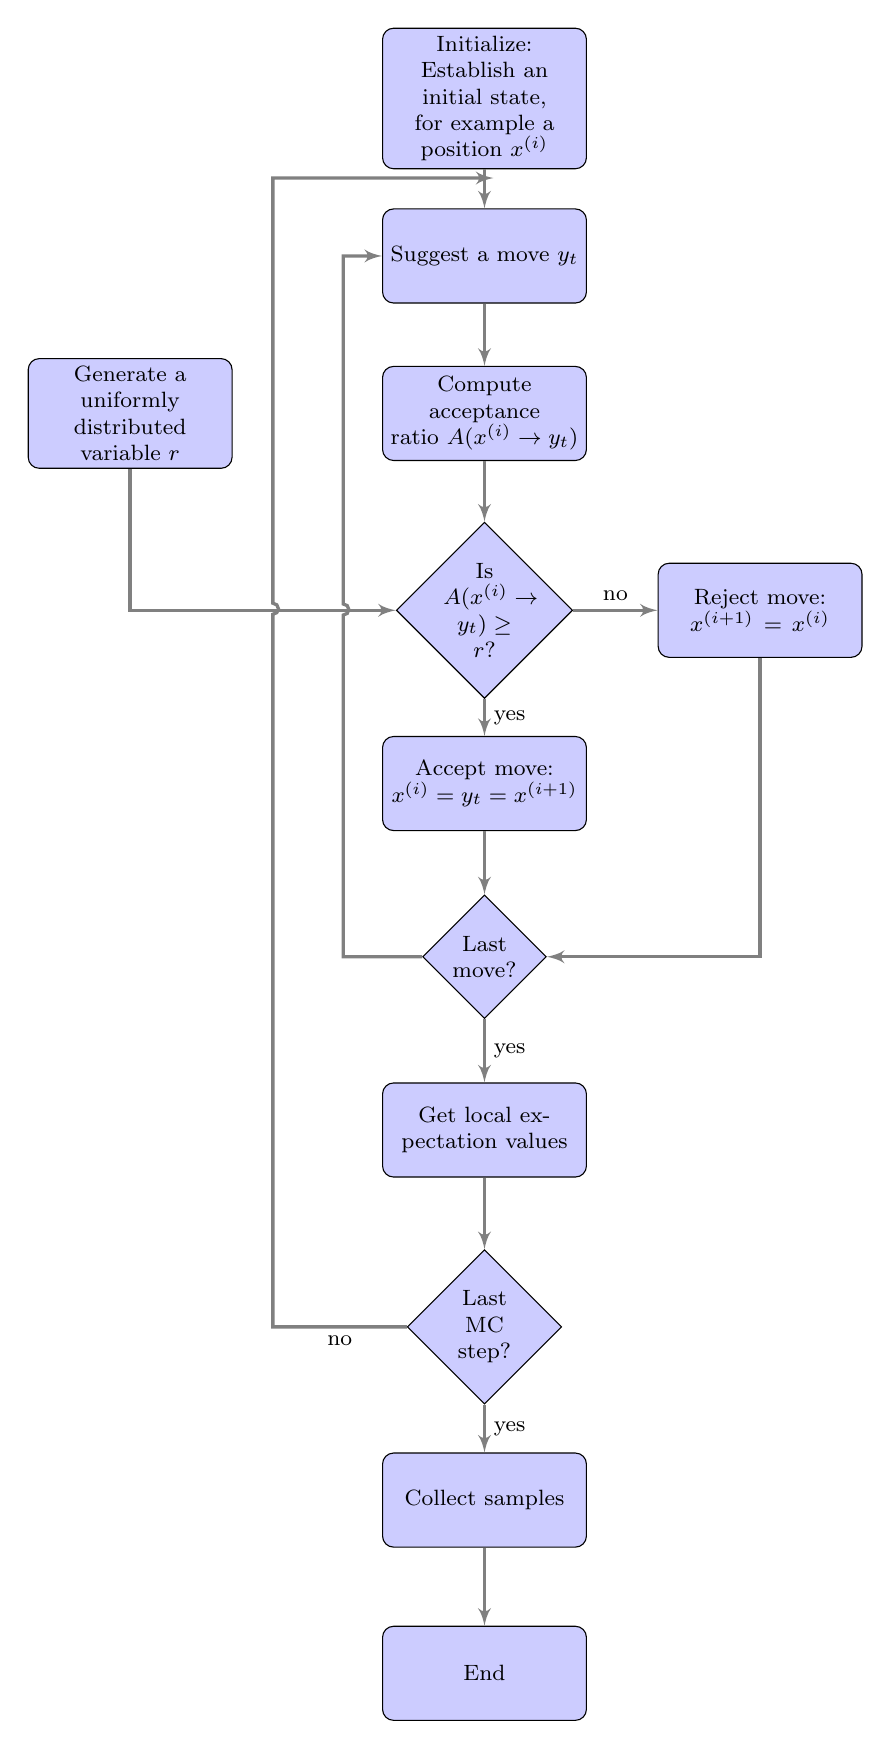
\begin{tikzpicture}[scale=1., node distance = 2cm, auto]
  \footnotesize
    % Place nodes
    \node [block] (init) {Initialize:\\
    Establish an initial state, for example a position $x^{(i)}$};
    \node [block, below of=init, node distance=2.0cm] (suggestMove) {Suggest a move $y_t$};
    \node [block, below of=suggestMove] (evaluateAcceptance) {Compute acceptance ratio $A(x^{(i)}\rightarrow y_t)$};
    \node [block, left of=evaluateAcceptance, node distance=4.5cm] (randomGenerator) {Generate a uniformly distributed variable $r$};
    \node [decision, below of=evaluateAcceptance] (decide) {Is\\ $A(x^{(i)}\rightarrow y_t) \geq r$?};
    \node [block, right of=decide, node distance=3.5 cm] (rejectMove) {Reject move: \\ $x^{(i+1)} = x^{(i)}$};
    \node [block, below of=decide, node distance=2.2cm] (acceptMove) {Accept move:\\$x^{(i)} = y_t=x^{(i+1)}$};
    \node [decision, below of=acceptMove, node distance=2.2cm] (lastMove) {Last move?};
    \node [block, below of=lastMove, node distance=2.2cm] (getLocalEnergy) {Get local expectation values};
    \node [decision, below of=getLocalEnergy] (decideMC) {Last MC step?};
    \node [block, below of=decideMC, node distance=2.2cm] (collectSamples) {Collect samples};
    \node [block, below of=collectSamples, node distance=2.2cm] (end) {End};
    
%     % Draw edges
    \path [line] (init) -- (suggestMove);
    \path [line] (suggestMove) -- (evaluateAcceptance);
    \path [line] (evaluateAcceptance) -- (decide);
    \path [line] (randomGenerator) |- (decide);
    \path [line] (decide) -- node [, color=black] {yes}(acceptMove);
    \path [line] (decide) -- node [, color=black] {no}(rejectMove);
    \path [line] (acceptMove) -- (lastMove); 
    \path [line] (lastMove) -- node [, color=black] {yes}(getLocalEnergy);
    \path [line] (rejectMove) |- (lastMove);
    \path [line] (getLocalEnergy) -- (decideMC);
    \path [line] (decideMC) -- node [, color=black] {yes}(collectSamples);

    % Define a style for shifting a coordinate upwards
    % Note the curly brackets around the coordinate.
    \tikzstyle{s}=[shift={(0mm,\radius)}]
    \path[line] (lastMove.west) -- +(-1.0,0)  -- +(-1.0, 4.34) 
% % % %     % Draw semicircle junction to indicate that the lines are
% % % %     % not connected. Since we want the semicircle to have its center 
% % % %     % where the lines intersect, we have to shift the intersection 
% % % %     % coordinate using the 's' style to account for this.
    arc(-90:90:\radius) -- +(0.0, 4.42) -- (suggestMove.west);
    
    \path [line] (decideMC.west) -- node [, color=black]{no} +(-1.7,0) --+(-1.7,9.05) arc(-90:90:\radius) --+(0.0,5.4) -- +(2.8,5.4);
       
    \path [line] (collectSamples) -- (end);

\end{tikzpicture}\caption{Chart flow for the Metropolis algorithm.}\label{fig:chartFlowMetro}
\end{centering}
\end{figure}


The dynamical equation can be written as
\begin{equation}
w_i(t+1) = \sum_j M_{ij}w_j(t)
\end{equation}
with the matrix $M$ given by
\begin{equation}
M_{ij} = \delta_{ij}\left [ 1 -\sum_k T_{i\rightarrow k} A_{i \rightarrow k}
\right ] + T_{j\rightarrow i} A_{j\rightarrow i} \,.
\end{equation}
Summing over $i$ shows that $\sum_i M_{ij} = 1$, and since
$\sum_k T_{i\rightarrow k} = 1$, and $A_{i \rightarrow k} \leq 1$, the
elements of the matrix satisfy $M_{ij} \geq 0$. The matrix $M$ is therefore
a stochastic matrix.

The Metropolis method is simply the power method for computing the
right eigenvector of $M$ with the largest magnitude eigenvalue.
By construction, the correct probability distribution is a right eigenvector
with eigenvalue $1$. Therefore, for the Metropolis method to converge
to this result, one has to  show that $M$ has only one eigenvalue with this
magnitude, and all other eigenvalues are smaller. 
%develop examples here or in chapter 7 in connection with power method


\section{Langevin and Fokker-Planck Equations}
We end this chapter with a discussion and derivation of the Fokker-Planck and Langevin equations.
These equations will in turn be used in our discussion on advanced Monte Carlo methods
for quantum mechanical systems, see chapter for example chapter \ref{chap:improvedvmc}.

\subsection{Fokker-Planck Equation}
     For many physical systems initial distributions of a stochastic 
variable $y$ tend to an equilibrium distribution $w_{\mathrm{equilibrium}}(y)$, 
that is $w(y, t)\rightarrow w_{\mathrm{equilibrium}}(y)$ 
as $t\rightarrow\infty$. In
equilibrium, detailed balance constrains the transition rates
\[
     W(y\rightarrow y')w(y ) = W(y'\rightarrow y)w_{\mathrm{equilibrium}}(y),
\]
where $W(y'\rightarrow y)$ 
is the probability per unit time that the system changes
from a state $|y\rangle$ , characterized by the value $y$ 
for the stochastic variable $Y$ , to a state $|y'\rangle$.

Note that for a system in equilibrium the transition rate 
$W(y'\rightarrow y)$ and
the reverse $W(y\rightarrow y')$ may be very different. 


Let us now assume that we have three probability distribution functions for times $t_0 < t' < t$, that is
$w({\bf x}_0,t_0)$, $w({\bf x}',t')$ and $w({\bf x},t)$.
We have then  
\[
   w({\bf x},t)= \int_{-\infty}^{\infty} W({\bf x}.t|{\bf x}'.t')w({\bf x}',t')d{\bf x}',
\]
and
\[
   w({\bf x},t)= \int_{-\infty}^{\infty} W({\bf x}.t|{\bf x}_0.t_0)w({\bf x}_0,t_0)d{\bf x}_0,
\]
and
\[
   w({\bf x}',t')= \int_{-\infty}^{\infty} W({\bf x}'.t'|{\bf x}_0,t_0)w({\bf x}_0,t_0)d{\bf x}_0.
\]

We can combine these equations and arrive at the 
famous Einstein-Smoluchenski-Kolmogorov-Chapman (ESKC) relation
\[
 W({\bf x}t|{\bf x}_0t_0)  = \int_{-\infty}^{\infty} W({\bf x},t|{\bf x}',t')W({\bf x}',t'|{\bf x}_0,t_0)d{\bf x}'.
\]
We can replace the spatial dependence with a dependence upon say the velocity
(or momentum), that is we have
\[
 W({\bf v},t|{\bf v}_0,t_0)  = \int_{-\infty}^{\infty} W({\bf v},t|{\bf v}',t')W({\bf v}',t'|{\bf v}_0,t_0)d{\bf x}'.
\]

We will now derive the Fokker-Planck equation. 
We start from the ESKC equation
\[
 W({\bf x},t|{\bf x}_0,t_0)  = \int_{-\infty}^{\infty} W({\bf x},t|{\bf x}',t')W({\bf x}',t'|{\bf x}_0,t_0)d{\bf x}'.
\]
We define $s=t'-t_0$, $\tau=t-t'$ and $t-t_0=s+\tau$. We have then
\[
 W({\bf x},s+\tau|{\bf x}_0)  = \int_{-\infty}^{\infty} W({\bf x},\tau|{\bf x}')W({\bf x}',s|{\bf x}_0)d{\bf x}'.
\]

Assume now that $\tau$ is very small so that we can make an expansion 
in terms of a small step $xi$, with ${\bf x}'={\bf x}-\xi$, that is
\[
 W({\bf x},s|{\bf x}_0)+\frac{\partial W}{\partial s}\tau +O(\tau^2) = \int_{-\infty}^{\infty} W({\bf x},\tau|{\bf x}-\xi)W({\bf x}-\xi,s|{\bf x}_0)d{\bf x}'.
\]
We assume that $W({\bf x},\tau|{\bf x}-\xi)$ takes non-negligible values only when $\xi$ is small. This is just another way of stating the Master equation!

We say thus that ${\bf x}$ changes only by a small amount in the time interval $\tau$. 
This means that we can make a Taylor expansion in terms of $\xi$, that is we
expand
\[
W({\bf x},\tau|{\bf x}-\xi)W({\bf x}-\xi,s|{\bf x}_0) =
\sum_{n=0}^{\infty}\frac{(-\xi)^n}{n!}\frac{\partial^n}{\partial x^n}\left[W({\bf x}+\xi,\tau|{\bf x})W({\bf x},s|{\bf x}_0)
\right].
\]
We can then rewrite the ESKC equation as 
\[
\frac{\partial W}{\partial s}\tau=-W({\bf x},s|{\bf x}_0)+
\sum_{n=0}^{\infty}\frac{(-\xi)^n}{n!}\frac{\partial^n}{\partial x^n}
\left[W({\bf x},s|{\bf x}_0)\int_{-\infty}^{\infty} \xi^nW({\bf x}+\xi,\tau|{\bf x})d\xi\right].
\]
We have neglected higher powers of $\tau$ and have used that for $n=0$ 
we get simply $W({\bf x},s|{\bf x}_0)$ due to normalization.

We say thus that ${\bf x}$ changes only by a small amount in the time interval $\tau$. 
This means that we can make a Taylor expansion in terms of $\xi$, that is we
expand
\[
W({\bf x},\tau|{\bf x}-\xi)W({\bf x}-\xi,s|{\bf x}_0) =
\sum_{n=0}^{\infty}\frac{(-\xi)^n}{n!}\frac{\partial^n}{\partial x^n}\left[W({\bf x}+\xi,\tau|{\bf x})W({\bf x},s|{\bf x}_0)
\right].
\]
We simplify the above by introducing the moments 
\[
M_n=\frac{1}{\tau}\int_{-\infty}^{\infty} \xi^nW({\bf x}+\xi,\tau|{\bf x})d\xi=
\frac{\langle [\Delta x(\tau)]^n\rangle}{\tau},
\]
resulting in
\[
\frac{\partial W({\bf x},s|{\bf x}_0)}{\partial s}=
\sum_{n=1}^{\infty}\frac{(-\xi)^n}{n!}\frac{\partial^n}{\partial x^n}
\left[W({\bf x},s|{\bf x}_0)M_n\right].
\]

When $\tau \rightarrow 0$ we assume that $\langle [\Delta x(\tau)]^n\rangle \rightarrow 0$ more rapidly than $\tau$ itself if $n > 2$. 
When $\tau$ is much larger than the standard correlation time of 
system then $M_n$ for $n > 2$ can normally be neglected.
This means that fluctuations become negligible at large time scales.

If we neglect such terms we can rewrite the ESKC equation as 
\[
\frac{\partial W({\bf x},s|{\bf x}_0)}{\partial s}=
-\frac{\partial M_1W({\bf x},s|{\bf x}_0)}{\partial x}+
\frac{1}{2}\frac{\partial^2 M_2W({\bf x},s|{\bf x}_0)}{\partial x^2}.
\]

In a more compact form we have
\[
\frac{\partial W}{\partial s}=
-\frac{\partial M_1W}{\partial x}+
\frac{1}{2}\frac{\partial^2 M_2W}{\partial x^2},
\]
which is the Fokker-Planck equation.  It is trivial to replace 
position with velocity (momentum).

The solution to this equation is a Gaussian distribution and can be used to constrain proposed transitions moves, that one can model the transition probabilities $T$ from our discussion of the Metropolis algorithm.
\subsection{Langevin Equation}
Consider a particle suspended in a liquid. 
On its path through the liquid it will continuously collide with the liquid molecules. 
Because on average the particle will collide more often on the front side than on the back side, it will experience a systematic force proportional with its velocity, 
and directed opposite to its velocity. Besides this 
systematic force the particle will experience a stochastic force  $ \vec{F}(t)$. 
The equations of motion then read 
\[ 
 \frac{d\vec{r}}{dt} 	=  \vec{v},
\] 	
\[
\frac{d\vec{v}}{dt} 	=  -\xi \vec{v}+\vec{F},
\]
The last equation is the Langevin equation. The original Langevin equation was meant to  describe 
Brownian motion. It is a 
stochastic differential equation used to describe the time evolution of 
collective (normally macroscopic) variables that change only slowly with respect
to the microscopic ones. The latter are responsible for the stochastic nature of the Langevin equation.
We can say that we model our ignorance about the microscopic physics in a stochastic term.
From the Langevin equation we can in turn derive for example the fluctuation dissipation theorem
discussed below. To see, we need some information about the friction constant from hydrodynamics.
From hydrodynamics  we know that the friction constant  $\xi$ is given by
\[
\xi =6\pi \eta a/m 
\]
where $\eta$ is the viscosity  of the solvent and $a$ is the radius of the particle.

Solving the Langevin equation we get 
\[
\vec{v}(t)=\vec{v}_{0}e^{-\xi t}+\int_{0}^{t}d\tau e^{-\xi (t-\tau )}\vec{F }(\tau ). 
\]

If we want to get some useful information out of this, we have to average 
over all possible realizations of 
$ \vec{F}(t)$, with the initial velocity as a condition. A useful quantity is then
 \[ 
\langle \vec{v}(t)\cdot \vec{v}(t)\rangle_{\vec{v}_{0}}=v_{0}^{-\xi 2t}
+2\int_{0}^{t}d\tau e^{-\xi (2t-\tau)}\vec{v}_{0}\cdot \langle \vec{F}(\tau )\rangle_{\vec{v}_{0}}
\]
\[  	  	
 +\int_{0}^{t}d\tau ^{\prime }\int_{0}^{t}d\tau e^{-\xi (2t-\tau -\tau ^{\prime })}
\langle \vec{F}(\tau )\cdot \vec{F}(\tau ^{\prime })\rangle_{ \vec{v}_{0}}.
\]

In order to continue we have to make some assumptions 
about the conditional averages of the stochastic forces. 
In view of the chaotic character of the stochastic forces the following 
assumptions seem to be appropriate.
We assume that   
\[ \langle \vec{F}(t)\rangle 	= 	0, \]
and
\[\langle \vec{F}(t)\cdot \vec{F}(t^{\prime })\rangle_{\vec{v}_{0}}=  C_{\vec{v}_{0}}\delta (t-t^{\prime }).
\] 	
We omit the subscript $\vec{v}_{0}$ when the quantity of interest 
turns out to be independent of $\vec{v}_{0}$. Using the last three equations we get
 \[
\langle \vec{v}(t)\cdot \vec{v}(t)\rangle_{\vec{v}_{0}}=v_{0}^{2}e^{-2\xi t}+\frac{C_{\vec{v}_{0}}}{2\xi }(1-e^{-2\xi t}).\]

For large $t$ this should be equal to the well-known result $3kT/m$, from which it follows that
\[
\langle \vec{F}(t)\cdot \vec{F}(t^{\prime })\rangle =6\frac{kT}{m}\xi \delta (t-t^{\prime }). \]
This result is called the fluctuation-dissipation theorem.

Integrating 
 \[ 
\vec{v}(t)=\vec{v}_{0}e^{-\xi t}+\int_{0}^{t}d\tau e^{-\xi (t-\tau )}\vec{F }(\tau ), \] 
we get
\[
\vec{r}(t)=\vec{r}_{0}+\vec{v}_{0}\frac{1}{\xi }(1-e^{-\xi t})+
\int_0^td\tau \int_0^{\tau}\tau ^{\prime } e^{-\xi (\tau -\tau ^{\prime })}\vec{F}(\tau ^{\prime }), \]
from which we calculate the mean square displacement 
\[
\langle ( \vec{r}(t)-\vec{r}_{0})^{2}\rangle _{\vec{v}_{0}}=\frac{v_0^2}{\xi}(1-e^{-\xi t})^{2}+\frac{3kT}{m\xi ^{2}}(2\xi t-3+4e^{-\xi t}-e^{-2\xi t}). \]
For very large $t$ this becomes
\[
\langle (\vec{r}(t)-\vec{r}_{0})^{2}\rangle =\frac{6kT}{m\xi }t \] 
from which we get the Einstein relation  
 \[ D= \frac{kT}{m\xi } \] 	
where we have used $\langle (\vec{r}(t)-\vec{r}_{0})^{2}\rangle =6Dt$.

The standard approach in for example quantum mechanical diffusion Monte Carlo calculations, is to use the Langevin equation
to propose new moves (for examples new velocities or positions) since they will depend on the given probability distributions.
These new proposed states or values are then used to compute the transition probability $T$, where the latter is the solution
of for example the Fokker-Planck equation.
 
\section{Exercises}
%\subsection*{Exercise 9.1: Two dimensional randow walk}
\begin{prob}
Extend the first program discussed in this chapter  
to a two-dimensional random walk with probability
$1/4$ for a move to the right, left, up or down. Compute the variance for both the $x$ and $y$
directions and the total variance.
\end{prob}
%\subsection*{Exercise 12.1: Two dimensional randow walk}
\begin{prob}
Use the second program 
to fit the computed probability distribution with a normal distribution
using your calculated values of $\sigma^2$ and $\langle x\rangle$.
\end{prob}
%\subsection*{Project 12.1: simulation of the Boltzmann distribution}
\begin{prob}
In this exercise the aim is to show that the Metropolis algorithm
generates the Boltzmann distribution
\[
   P(\beta)=\frac{e^{-\beta E}}{Z},
\]
with $\beta=1/kT$ being the inverse temperature, $E$ is the energy of
the system and
$Z$ is the partition function. The only functions you will need are those
to generate random numbers.

We are going to study one single particle in equilibrium with 
its surroundings, the latter modelled via a large heat bath
with temperature $T$.

The model used to describe this particle is that of an ideal gas
in {\bf one} dimension and with velocity $-v$ or $v$. 
We are interested in finding  $P(v)dv$, which expresses the probability
for finding the system with a given velocity $v\in [v,v+dv]$.
The energy for this one-dimensional system is
\[
  E=\frac{1}{2}kT=\frac{1}{2}v^2,
\]
with mass $m=1$.
In order to simulate the Boltzmann distribution, your program
should contain the following ingredients:  
\begin{itemize}
\item Reads in the temperature $T$, the number of Monte Carlo cycles, 
and the initial velocity. You should also read in 
the change in velocity $\delta v$ used in every Monte Carlo step. 
Let the temperature have dimension energy.
\item Thereafter you choose a maximum velocity given by for example  
$v_{max}\sim 10\sqrt{T}$. This should include all relevant velocities which give a non-zero probability. But you need to check whether this is true or not. 

Then you construct a velocity interval 
defined by  $v_{max}$ and divide it in small intervals through 
$v_{max}/N$,
with $N\sim 100-1000$. 
For each of these intervals your task is to find out how many times
a given velocity during the Monte Carlo sampling appears 
in each specific interval.
\item The number of times a given velocity appears in a specific
interval is used to construct a histogram representing 
$P(v)dv$. To achieve this you should construct a vector 
$P[N]$ which contains the number of times a given velocity 
appears in the subinterval 
$v,v+dv$. 
\end{itemize}

In order to find the number of velocities appearing in each interval
we will employ the Metropolis algorithm. A pseudocode for this is
\begin{lstlisting}
   for( montecarlo_cycles=1; Max_cycles; montecarlo_cycles++) {
      ...
      // change speed as function of delta v
      v_change = (2*ran1(&idum) -1 )* delta_v;
      v_new = v_old+v_change;
      // energy change
      delta_E = 0.5*(v_new*v_new - v_old*v_old) ;
      ......
      // Metropolis algorithm begins here
        if ( ran1(&idum) <= exp(-beta*delta_E)  ) {
            accept_step = accept_step + 1 ;      
            v_old = v_new ;
            .....
        }
      // thereafter we must fill in  P[N] as a function of
      // the new speed
        P[?] = ...

      // upgrade mean velocity, energy and variance
         ...
      }
\end{lstlisting}


\begin{enumerate}
\item  Make your own algorithm which sets up the histogram
$P(v)dv$, find mean velocity, energy $\langle E\rangle$, energy variance $\mathrm{Var}(E)$ 
and the number of
accepted steps for a given temperature. Study the change of the number of
accepted moves as a function of $\delta v$.
Compare the final energy with the closed form result
$\langle E\rangle=kT/2$ for one dimension. Find also the closed-form expressions for the energy variance  and the mean velocity and compare your calculations with these results. 
Use $T=4$ and set the intial velocity to zero, i.e., $v_0=0$. 
Try different values of $\delta v$.
Check the final result for the energy as a function 
of the number of Monte Carlo cycles.

\item   Repeat the calculation in the previous exercise but using now a normal distribution. Does that improve your results compared with the exact expressions?

\item  Make thereafter a plot of  $\log{(P(v))}$ as function of $E$
and see if you get a straight line. Comment the result.

\item  In our analysis under [1) we have not discussed how the system reaches the most likely state, that is whether equilibrium has been reached or not.
Make a plot of the mean velocity, energy, energy variance and the number of
accepted steps for a given temperature as function of the number of
Monte Carlo samples. Perform these calculations for several temperatures, namely $T=0.5$, $T=1$, $T=2$ and $T=10$ and comment your results. Can you find
a rough measure for when the most likely state has been reached?

\item 
The analysis in point [4) 
is rather rough and obviously user dependent, in the sense that it is
very much up to the user to define when an equilibrium situation has been reached or not.
To improve upon this, compute the so-called time autocorrelation function defined here as
\[
\phi(t)  = \frac{1}{t_{\mathrm{max}}-t}\sum_{t'=0}^{t_{\mathrm{max}}-t}\bar E(t')\bar E(t'+t)
-\frac{1}{t_{\mathrm{max}}-t}\sum_{t'=0}^{t_{\mathrm{max}}-t}\bar E(t')\times
\frac{1}{t_{\mathrm{max}}-t}\sum_{t'=0}^{t_{\mathrm{max}}-t}\bar E(t'+t)
\]
for the mean energy $E\bar (t)$ and plot it 
as function of the number of Monte Carlo steps for the temperatures in [c).
The time $t$ corresponds to a given number of Monte Carlo cycles.
Can you extract an equilibration measure?  How does the correlation time behave
as function of temperature?  Comment your results.  
Be careful in choosing values of $t$, they should not be  too close to $t_{\mathrm{max}}$.
Compute the autocorrelation function for all temperatures listed in [d) and compare your results with those in [d). Comment your results. 
\item  In the previous analysis we computed the time autocorrelation  function. This quantity can be related to the covariance of our measurements. 
To achieve this you need to store the results of all contributions to the measurements of the mean energy and its variance $\sigma_E^2$ given by     
\[
\sigma_E^2 =\frac{1}{n^2}\sum_{k=1}^n (E_k - \bar E)^2 +
\frac{2}{n^2}\sum_{k<l} (E_k - \bar E)(E_l - \bar E)
\]
Here we assume that $n$ corresponds to the number of Monte Carlo samples in one
experiment and that we repeat these experiments a given time.  We can assume here that we repeat these experiments $m=n$ times.  
The value $\bar E$ is the mean energy while $E_{k,l}$ represent individual measurements. 
The first term is the same as the error in the uncorrelated case.
This means that the second
term accounts for the error correction due to correlation between the
measurements. For uncorrelated measurements this second term is zero.

Computationally the uncorrelated first term is much easier to treat
efficiently than the second.
\[
\mathrm{Var}(E) = \frac{1}{n}\sum_{k=1}^n (E_k - \langle E\rangle)^2 =
\left(\frac{1}{n}\sum_{k=1}^n E_k^2\right) - \langle E\rangle^2
\]
We just accumulate separately the values $E_k^2$ and $E_k$ for every
measurement $E_k$ we receive. The correlation term, though, has to be
calculated at the end of the experiment since we need all the
measurements to calculate the cross terms. Therefore, all measurements
have to be stored throughout the experiment.

Let us analyze the problem by splitting up the correlation term into
partial sums of the form:
\[
f_d = \frac{1}{n}\sum_{k=1}^{n-d}(E_k - \langle E\rangle)(E_{k+d} - \langle E\rangle)
\]
The correlation term of the error can now be rewritten in terms of
$f_d$:
\[
\frac{2}{n}\sum_{k<l} (E_k - \langle E\rangle)(E_l - \langle E\rangle) =
2\sum_{d=1}^{n-1} f_d
\]
The value of $f_d$ reflects the correlation between measurements
separated by the distance $d$ in the samples.  Notice that for
$d=0$, $f$ is just the sample variance, $\mathrm{Var}(E)$. If we divide $f_d$
by $\mathrm{Var}(E)$, we arrive at the so called \emph{autocorrelation
  function}:
\[
\kappa_d = \frac{f_d}{\mathrm{Var}(E)}
\]
which gives us a useful measure of the correlation pair correlation
starting always at $1$ for $d=0$.

The sample variance can now be
written in terms of the autocorrelation function:
\bea
\sigma_E^2 &=&
\frac{1}{n}\mathrm{Var}(E)+\frac{2}{n}\cdot\mathrm{Var}(E)\sum_{d=1}^{n-1}
\frac{f_d}{\mathrm{Var}(E)}\nonumber\\ &=&
\left(1+2\sum_{d=1}^{n-1}\kappa_d\right)\frac{1}{n}\mathrm{Var}(E)\nonumber\\
&=&\rule{0pt}{17pt}
\frac{\tau}{n}\cdot\mathrm{Var}(E)
\label{eq:error_estimate_corr_new}
\eea
and we see that $\sigma_E^2$ can be expressed in terms the
uncorrelated sample variance times a correction factor $\tau$ which
accounts for the correlation between measurements. We call this
correction factor the \emph{autocorrelation time}:
\[
\tau = 1+2\sum_{d=1}^{n-1}\kappa_d
\]
%It is closely related to the area under the graph of the
%autocorrelation function. 
For a correlation free experiment, $\tau$
equals 1. From the point of view of
Eq.~(\ref{eq:error_estimate_corr_new}) we can interpret a sequential
correlation as an effective reduction of the number of measurements by
a factor $\tau$. The effective number of measurements becomes
\bdm
n_\mathrm{eff} = \frac{n}{\tau}
\edm
From the previous exercise you needed to store all experiments $E_k$ in order to compute the time autocorrelation function. You can reuse these data in this exercise and compute the full variance $\sigma_E^2$, the covariance, the 
autocorrelation time $\tau$ and the effective number of measurements
$n_\mathrm{eff}$. It is sufficient to choose only one of the temperatures.  Comment your results.
Can you relate the correlation time $\tau$ to what you found [5)? What about the covariance and the time autocorrelation function? 

\end{enumerate}

\end{prob}


\begin{prob}


The aim of this exercise is to simulate financial transactions among financial agents
using Monte Carlo methods. The final goal is to extract a distribution of income  as function
of the income $m$.   From Pareto's work (V.~Pareto, 1897) it is known from empirical studies
that the higher end of the distribution of money follows a distribution 
\[
w_m\propto m^{-1-\alpha},
\]
with $\alpha\in [1,2]$. We will here follow the analysis made by Patriarca {\em et al} \cite{patriarca2004}. 

Here we will study numerically the relation between the microdynamical 
relations among financial 
agents and the  resulting macroscopic money distribution.

We assume we have $N$ agents that exchange money in pairs $(i,j)$. We assume also that all agents
start with the same amount of money $m_0 > 0$. At a given 'time step', we choose randomly a pair
of agents $(i,j)$ and let a transaction take place. This means that agent $i$'s money $m_i$ changes
to $m_i'$ and similarly we have $m_j\rightarrow m_j'$. 
Money is conserved during a transaction, meaning that
\begin{equation}
m_i+m_j=m_i'+m_j'.
\label{eq:conserve}
\end{equation}
The change is done via a random reassignement (a random number) $\epsilon$, meaning that
\[
m_i' = \epsilon(m_i+m_j),
\]
leading to
\[
m_j'= (1-\epsilon)(m_i+m_j).
\]
The number $\epsilon$ is extracted from a uniform distribution. 
In this simple model, no agents are left with a debt, that is $m\ge 0$. 
Due to the conservation law above, one can show that the system relaxes toward an equilibrium
state given by a Gibbs distribution
\[
   w_m=\beta \exp{(-\beta m)},
\]
with 
\[
\beta = \frac{1}{\langle m\rangle},
\]
and $\langle m\rangle=\sum_i m_i/N=m_0$, the average money.
It means that after equilibrium has been reached that the majority of agents is left with a small 
number of money, while the number of richest agents, those with $m$ larger than a specific value $m'$,
exponentially decreases with $m'$. 

We assume that we have $N=500$ agents.   In each simulation, we need a sufficiently large number of transactions, say $10^7$. Our aim is find the final equilibrium distribution $w_m$. In order to do that we would need
several runs of the above simulations, at least $10^3-10^4$ runs (experiments).  


\begin{enumerate}
\item[a)] Your task is to first set up an algorithm which simulates the above transactions with an initial
amount $m_0$.
The challenge here is to figure out a Monte Carlo  simulation  based on the
above equations.  
You will in particular need to make an algorithm which sets up a histogram as function of $m$.
This histogram contains the number of times a value $m$ is registered and represents
$w_m\Delta m$. You will need to set up a value for the interval $\Delta m$  (typically $0.01-0.05$).
That means you need to account for the number of times you register an income in the interval
$m,m+\Delta m$. The number of times you register this income, represents the value that enters the histogram.
You will also need to find a criterion for when the equilibrium situation has been reached.

\item[b)] Make thereafter a plot of  $\log{(w_m)}$ as function of $m$
and see if you get a straight line. 
Comment the result.

\item[c)] We can then change our model to allow for a saving criterion, meaning that the agents save
a fraction $\lambda$ of the money they have before the transaction is made. The final distribution will then no longer be given by Gibbs distribution. It could also include a taxation on financial transactions.

The conservation law of Eq.~(\ref{eq:conserve}) holds, but the money to be shared in a transaction between
agent $i$ and agent $j$ is now $(1-\lambda)(m_i+m_j)$. This means that we have 
\[
m_i' = \lambda m_i+\epsilon(1-\lambda)(m_i+m_j),
\]
and 
\[
m_j' = \lambda m_j+(1-\epsilon)(1-\lambda)(m_i+m_j),
\]
which can be written as 
\[
m_i'=m_i+\delta m
\]
and 
\[
m_j'=m_j-\delta m,
\]
with 
\[
\delta m=(1-\lambda)(\epsilon m_j-(1-\epsilon)m_i),
\]
showing how money is conserved during a transaction.
Select values of $\lambda =0.25,0.5$ and $\lambda=0.9$ and try to extract the corresponding
equilibrium distributions and compare these with the Gibbs distribution. Comment your results.
If you have time, see if you can extract a parametrization of the above curves (see 
Patriarca {\em et al} \cite{patriarca2004}) 
\end{enumerate}

\end{prob}




 \clearemptydoublepage
%  last update 22/10/2006

%  correct several typos on closed-form soultions
%  present solution to the Potts model
%  add about cluster models, wolff's algo
%  add about finite size scaling, show derivation of results

\chapter{Monte Carlo Methods in Statistical Physics}\label{chap:mcstat} 

\begin{quotation}
When you are solving a problem, don't worry. Now, after you have solved the problem, then that's the time to worry. {\em Richard Feynman}
\end{quotation}
\abstract{The aim of this chapter is to present examples from the 
physical sciences where Monte Carlo methods are widely applied.
Here we focus on examples from statistical physics
and discuss 
two of the most studied models, the Ising model and the Potts model for the interaction
among classical spins. These models have been widely used for studies of phase transitions. }

\section{Introduction and Motivation}

Fluctuations play a central role in our understanding of phase transitions. Their behavior
near critical points convey important information about the underlying many-particle 
interactions. In this chapter we will focus on two widely studied models in statistical physics,
the Ising model and the Potts model for interacting spins. The main focus is on the Ising model. 
Both models can exhibit first and second
order phase transitions and are perhaps among the most studied
systems in statistical physics with respect to 
simulations of phase transitions. 
The Norwegian-born chemist 
Lars Onsager  developed in 1944 an ingenious mathematical  
description of the Ising model \cite{onsager1944} meant to simulate a 
 two-dimensional model of a magnet composed of many small atomic magnets. 
This work proved later useful in analyzing other complex systems, 
such as gases sticking to solid surfaces, and hemoglobin molecules that absorb oxygen. 
He got the Nobel prize in chemistry in 1968 for his studies  of 
non-equilibrium thermodynamics. Many people argue he should have received the Nobel prize in physics as well for
his work on the Ising model.
Another model we discuss at the end of this chapter is the so-called class 
of Potts models, which exhibits both first and second order type of phase transitions.
Both the Ising model and the Potts  model have been used to model phase transitions in
solid state physics, with a particular emphasis on ferromagnetism and antiferromagnetism.

Metals like 
iron, nickel, cobalt and some of the rare earths (gadolinium, dysprosium) exhibit a 
unique magnetic behavior which is called ferromagnetism because iron (ferrum in Latin) is 
the most common and most dramatic example. 
Ferromagnetic materials exhibit a long-range ordering phenomenon at the atomic level which causes 
the unpaired electron spins to line up parallel with each other in a region called a domain. 
The long range order which creates magnetic domains in ferromagnetic materials arises from a quantum 
mechanical interaction at the atomic level. This interaction is remarkable in that it locks 
the magnetic moments of neighboring atoms into a rigid parallel order over a large number of atoms in spite of 
the thermal agitation which tends to randomize any atomic-level order. Sizes of domains range from a 0.1 mm to a 
few mm. When an external magnetic field is applied, the domains already aligned in the direction of this 
grow at the expense of their neighbors. 
For a given ferromagnetic material the long range order abruptly disappears at a certain temperature 
which is called the Curie temperature for the material. The Curie temperature of iron is about 1043 K while metals like
cobalt and nickel have a Curie temperature of 1388 K and 627 K, respectively, and some of the rare earth metals like gadolinium
and dysprosium have 293 K and 85 K, respectively.
We could think of an actual metal as composed of for example a cubic lattice with atoms at each corner
with a resulting magnetic moment pointing in a particular direction, as portrayed in Fig.~\ref{fig:latticefig}. 
\begin{figure}[btp]
\begin{center}
\begin{picture}(100,260)
\setlength{\unitlength}{1mm}
\put(50,0){\circle*{4}}
\put(0,0){\circle*{4}}
\put(35,35){\circle*{4}}
\put(35,85){\circle*{4}}
\put(50,50){\circle*{4}}
\put(85,85){\circle*{4}}
\put(85,35){\circle*{4}}
\put(0,50){\circle*{4}}
\thicklines
\put(0,0){\vector(-1,1){5}}
\put(0,50){\vector(-1,1){5}}
\put(50,0){\vector(-1,1){5}}
\put(35,35){\vector(-1,1){5}}
\put(35,85){\vector(-1,1){5}}
\put(85,35){\vector(-1,1){5}}
\put(85,85){\vector(-1,1){5}}
\put(50,50){\vector(-1,1){5}}
\dottedline{0.5}(0,0)(50,0)
\dottedline{2}(0,0)(35,35)
\dottedline{2}(35,35)(85,35)
\dottedline{0.5}(50,0)(85,35)
\dottedline{0.5}(0,0)(0,50)
\dottedline{0.5}(50,0)(50,50)
\dottedline{2}(35,35)(35,85)
\dottedline{0.5}(0,50)(50,50)
\dottedline{0.5}(0,50)(35,85)
\dottedline{0.5}(50,50)(85,85)
\dottedline{0.5}(35,85)(85,85)
\dottedline{0.5}(85,35)(85,85)
\end{picture}
\end{center}
\caption{Example of a cubic lattice with atoms at each corner. Each atom has a finite magnetic moment which 
points in a particular direction. \label{fig:latticefig}}.
\end{figure}
In many respects, these atomic magnets are like ordinary magnets and 
can be thought of in terms of little magnet vectors pointing from south to north poles.
The Ising model provides a simple way of describing how a magnetic material responds to thermal 
energy and an external magnetic field.  
In this model, each domain has a corresponding spin of north or south.  
The spins can be thought of as the poles of a bar magnet. 
The model assigns a value of +1 or -1 to the spins north and south respectively.  
The direction of the spins influences the total potential energy of the system.  

Another physical case where the application of the Ising model enjoys considerable
success is the description of 
antiferromagnetism. This is a 
type of magnetism where adjacent ions 
spontaneously 
align themselves at relatively low temperatures into opposite, or antiparallel, 
arrangements throughout the material so that it exhibits almost no gross external magnetism. 
In antiferromagnetic materials, which include certain metals and alloys in addition to some ionic solids, 
the magnetism from magnetic atoms or ions oriented in one direction is canceled out by the set of 
magnetic atoms or ions that are aligned in the reverse direction.

This spontaneous antiparallel coupling of atomic magnets is disrupted by heating and disappears entirely 
above a certain temperature, called the N�el temperature, characteristic of each antiferromagnetic material. 
(The N�el temperature is named for Louis N�el, French physicist, who in 1936 gave one of the 
first explanations of antiferromagnetism.) Some antiferromagnetic materials have N�el temperatures at, 
or even several hundred degrees above, room temperature, but usually these temperatures are lower. 
The N�el temperature for manganese oxide, for example, is 122 K.

Antiferromagnetic solids exhibit special behaviour in an applied magnetic field depending upon the temperature. 
At very low temperatures, the solid exhibits no response to the external field, because the antiparallel 
ordering of atomic magnets is rigidly maintained. At higher temperatures, 
some atoms break free of the orderly arrangement and align with the external field. 
This alignment and the weak magnetism it produces in the solid reach their peak at the N�el temperature. 
Above this temperature, thermal agitation progressively prevents alignment of the atoms with the magnetic field, 
so that the weak magnetism produced in the solid by the alignment of its atoms continuously decreases as temperature is increased. 
For further discussion of magnetic properties and solid state physics, see for example the text of Ashcroft and
Mermin \cite{mermin}.

As mentioned above, spin models like the Ising and Potts models can be used to model other systems as well,
such as gases sticking to solid surfaces, and hemoglobin molecules that absorb oxygen. We sketch such an application
in Fig.~\ref{fig:latticefig2}. 
\begin{figure}
\begin{center}
\begin{picture}(100,100)(-1,-1)
\setlength{\unitlength}{1mm}
\thicklines
\matrixput(0,0)(10,0){7}(0,10){4}{\circle{2}}
\matrixput(10,0)(20,0){3}(0,20){2}{\circle*{2}}
\matrixput(0,10)(20,0){4}(0,20){2}{\circle*{2}}
\matrixput(1,0)(10,0){6}(0,10){4}{\line(1,0){8}}
\matrixput(0,1)(10,0){7}(0,10){3}{\line(0,1){8}}
\end{picture}
\end{center}
\caption{The open (white) circles at each lattice point can represent a vacant site, while the black circles can represent the absorption of an atom on a metal surface. \label{fig:latticefig2}}.
\end{figure}


However,  before we present the Ising model, 
we feel it is appropriate to refresh  some important quantities
in statistical physics, such as various definitions of statistical ensembles, 
their partition functions
and relevant variables. 



\section{Review of Statistical Physics}



In statistical physics the concept of an ensemble is one of the cornerstones in the definition of
thermodynamical quantities. An ensemble is a collection of microphysics systems from which we derive 
expectations values and thermodynamical properties related to experiment. 
As an example, the specific heat (which is a measurable quantity in the laboratory) of a system of infinitely many particles, 
can be derived from the basic interactions
between the microscopic constituents. The latter can span from electrons to atoms and  molecules or a system of classical
spins. All these microscopic constituents  interact via a well-defined interaction.
We say therefore that statistical physics bridges the gap between the microscopic world and the macroscopic world.
Thermodynamical quantities such as the specific heat or net magnetization of a system can all be derived
from a microscopic theory.

There are several types of ensembles, with their pertinent expectaction values and potentials.
Table \ref{tab:listensembles} lists the most used ensembles in statistical physics together with frequently arising 
extensive
(depend on the size of the systems such as the number of particles) and intensive variables 
(apply to all components of a system),
in addition to associated potentials. 
\begin{table}[htb]
\caption{Overview of the most common ensembles and their  variables.
Here we have define $\cal M$ - to be the  magnetization, $\cal D$ - the electric
dipole moment, $\cal H$ - the magnetic field and $\cal E$ - to be the electric field. 
The last two replace the pressure as an intensive variable, while the magnetisation and
the dipole moment play the same role as volume, viz they are extensive 
variables. The invers temperatur $\beta$ regulates the mean energy while the chemical
potential $\mu$ regulates the mean number of particles.\label{tab:listensembles}}
\begin{center}
\begin{tabular}{|l|c|c|c|c|}
\hline
&&&&\\
&\multicolumn{1}{|c}{Microcanonical}&\multicolumn{1}{|c}{Canonical}&
\multicolumn{1}{|c}{Grand canonical}&\multicolumn{1}{|c|}{Pressure canonical}\\
&&&&\\
\hline 
&&&&\\
Exchange of heat  &no&yes&yes&yes\\
with the environment&&&&\\
&&&&\\
Exchange of particles&no&no&yes&no\\
with the environemt&&&&\\
&&&&\\
Thermodynamical&$V, \cal M, \cal D$&$V, \cal M, \cal D$&$V, \cal M, \cal D$
&$P, \cal H, \cal E$\\
parameters&     $E$&$T$&$T$&$T$\\
	    &$N$&$N$&$\mu$&$N$\\
&&&&\\
Potential& Entropy& Helmholtz & $PV$ & Gibbs\\
&&&&\\
Energy &Internal& Internal & Internal & Enthalpy\\
&&&&\\

&&&&\\
&&&&\\ \hline
\end{tabular}
\end{center}
\end{table}


\subsection{Microcanonical Ensemble}
The microcanonical ensemble represents an hypothetically isolated system such as a nucleus which does not exchange 
energy or particles via the environment. The thermodynamical quantity of interest is the entropy $S$ which is related to
the logarithm of the number of possible microscopic states $\Omega(E)$ at a given energy $E$ that 
the system can access. The relation is 
%&\multicolumn{1}{c|}{Mikrocanoninal, $\Omega (N, V, E)$}\\ 
\[ S=k_{B}ln\Omega.\]
When the system is in its ground state the entropy is zero since there is only one possible
ground state. For excited states, we can have a higher degeneracy than one and thus an entropy which is larger than zero.
We may therefore loosely state that the entropy measures the degree of order in a system.
At low energies, we expect that we have only few states which are accessible and that the system
prefers a specific ordering. At higher energies, more states become accessible and the entropy 
increases. 
The entropy can  be used to compute observables such as the temperature 
\[ \frac{1}{k_{B}T}=\left(\frac{\partial \log\Omega}{\partial E}\right)_{N, V},\]
the pressure
\[ \frac{p}{k_{B}T}=\left(\frac{\partial \log\Omega}{\partial V}\right)_{N, E},\]
or the chemical potential.
\[ \frac{\mu}{k_{B}T}=-\left(\frac{\partial \log\Omega}{\partial N}\right)_{V, E}.\]
It is very difficult to compute the density of states $\Omega(E)$ and thereby the partition function in
the microcanonical ensemble at a given energy $E$, since this
requires the knowledge of all possible microstates at a given energy. 
This means that calculations are seldomly done in the microcanonical ensemble.
In addition, since the microcanonical
ensemble is an isolated system, it is hard to give a physical meaning to a quantity like the microcanonical
temperature. 

\subsection{Canonical Ensemble}
One of the most used ensembles is the canonical one, which is related to the microcanonical ensemble
via a Legendre transformation. The temperature is an intensive variable in this ensemble whereas the energy
follows as an expectation value. 
In order to calculate expectation values such as the mean energy
$\langle E \rangle $
at a given temperature, we need a probability distribution.
It is given by the Boltzmann distribution 
\[
  P_i(\beta) = \frac{e^{-\beta E_i}}{Z}
\]
with $\beta=1/k_BT$ being the inverse temperature, $k_B$ is the 
Boltzmann constant, $E_i$ is the energy of a microstate $i$ while 
$Z$ is the partition function for the canonical ensemble
defined as
\[
Z=\sum_{i=1}^{M}e^{-\beta E_i},
\]
where the sum extends over all microstates
$M$. 
The potential of interest in this case is Helmholtz' free energy. It relates the expectation value of the
energy at a given temperatur $T$ to the entropy at the same temperature via
\[ F=-k_{B}TlnZ=\langle E \rangle-TS.\]
Helmholtz' free energy expresses the struggle between 
two important principles in physics, namely the strive towards an energy minimum and
the drive towards higher entropy as the temperature increases. A higher entropy may be interpreted as a larger degree
of disorder. When equilibrium is reached at a given temperature, we have a balance between these two principles.
The numerical expression is Helmholtz' free energy.
The creation of a macroscopic magnetic field from a bunch of atom-sized mini-magnets, as shown in 
Fig.~\ref{fig:latticefig} 
results from a careful balance between these two somewhat opposing principles in physics, order vs.~disorder.

In the canonical ensemble the entropy is given by
\[ S =k_{B}lnZ
+k_{B}T\left(\frac{\partial lnZ}{\partial T}\right)_{N, V},\]
and the pressure by
\[ p=k_{B}T\left(\frac{\partial lnZ}{\partial V}\right)_{N, T}.\]
Similarly we can compute the chemical potential as 
\[ \mu =-k_{B}T\left(\frac{\partial lnZ}{\partial N}\right)_{V, T}.\]

For a system described by the canonical ensemble, the energy is an
expectation value since we allow energy to be exchanged with the surroundings
(a heat bath with temperature $T$). 

This expectation value, the mean energy,
can be calculated using 
\[\langle E\rangle  =k_{B}T^{2}\left(\frac{\partial lnZ}{\partial T}\right)_{V, N}\]
or 
using the probability distribution
$P_i$ as
\[
  \langle E \rangle = \sum_{i=1}^M E_i P_i(\beta)= 
  \frac{1}{Z}\sum_{i=1}^M E_ie^{-\beta E_i}.
\]
The energy is proportional to the first derivative of the potential, Helmholtz' free energy.
The corresponding variance is defined as
\[
\sigma_E^2=\langle E^2 \rangle-\langle E \rangle^2=
         \frac{1}{Z}\sum_{i=1}^M E_i^2e^{-\beta E_i}-
          \left(\frac{1}{Z}\sum_{i=1}^M E_ie^{-\beta E_i}\right)^2.
\]
If we divide the latter quantity with
$kT^2$ we obtain the specific heat at constant volume 
\[
   C_V= \frac{1}{k_BT^2}\left(\langle E^2 \rangle-\langle E \rangle^2\right),
\]
which again can be related to the second derivative of Helmholtz' free energy.
Using the same prescription, we can also evaluate the mean magnetization
through 
\[
  \langle {\cal M} \rangle = \sum_i^M {\cal M}_i P_i(\beta)= 
  \frac{1}{Z}\sum_i^M {\cal M}_ie^{-\beta E_i},
\]
and the corresponding variance
\[
\sigma_{{\cal M}}^2=\langle {\cal M}^2 \rangle-\langle {\cal M} \rangle^2=
         \frac{1}{Z}\sum_{i=1}^M {\cal M}_i^2e^{-\beta E_i}-
          \left(\frac{1}{Z}\sum_{i=1}^M {\cal M}_ie^{-\beta E_i}\right)^2.
\]
This quantity defines also the susceptibility 
$\chi$ 
\[
  \chi=\frac{1}{k_BT}\left(\langle {\cal M}^2 \rangle-\langle {\cal M} \rangle^2\right).
\]

\subsection{Grand Canonical and Pressure Canonical} 
Two other ensembles which are much used in statistical physics and thermodynamics are the grand canonical and pressure
canonical ensembles. In the first
we allow the system (in contact with a large heat bath) 
to exchange both heat and particles with the environment.
The potential is, with a partition function $\Xi (V, T, \mu)$ with variables 
$V,T$ and $\mu$,
\[ pV=k_{B}Tln\Xi,\]
and the entropy is given by
\[ S =k_{B}ln\Xi 
+k_{B}T\left(\frac{\partial ln\Xi}{\partial T}\right)_{V, \mu},\]
while the mean number of particles is 
\[ \langle N\rangle  =k_{B}T\left(\frac{\partial ln\Xi}{\partial \mu}\right)_{V, T}.\]
The pressure is determined  as 
\[ p =k_{B}T\left(\frac{\partial ln\Xi}{\partial V}\right)_{\mu, T}.\]

In the pressure canonical ensemble we employ with Gibbs' free energy as the potential. It is related to
Helmholtz' free energy via $G=F+pV$. The partition function is 
$\Delta (N, p, T)$, with temperature, pressure and the number of particles as variables.
The pressure and volume term can be replaced by other external potentials, such as an external magnetic
field (or a gravitational field) which performs work on the system. Gibbs' free energy reads
\[ G=-k_{B}Tln\Delta,\]
and the entropy is given by
\[ S =k_{B}ln\Delta 
+k_{B}T\left(\frac{\partial ln\Delta}{\partial T}\right)_{p, N}.\]
We can compute the volume as 
\[ V =-k_{B}T\left(\frac{\partial ln\Delta}{\partial p}\right)_{N, T},\]
and finally the chemical potential
\[ \mu =-k_{B}T\left(\frac{\partial ln\Delta}{\partial N}\right)_{p, T}.\]

In this chapter we work with the canonical ensemble only.

\section{Ising Model and Phase Transitions in  Magnetic Systems}

\subsection{Theoretical Background}

The model we will employ in our studies of phase transitions at finite temperature for 
magnetic systems is the so-called Ising model. In its simplest form
the energy is expressed as
\[
  E=-J\sum_{<kl>}^{N}s_ks_l-{\cal B}\sum_k^Ns_k,
\]
with  $s_k=\pm 1$, $N$ is the total number of spins, 
$J$ is a coupling constant expressing the strength of the interaction
between neighboring spins and 
${\cal B}$ is an external magnetic field interacting with the magnetic
moment set up by the spins.
The symbol $<kl>$ indicates that we sum over nearest
neighbors only. 
Notice that for $J>0$ it is energetically favorable for neighboring spins 
to be aligned. This feature leads to, at low enough temperatures,
a cooperative phenomenon called spontaneous magnetization. That is, 
through interactions between nearest neighbors, a given magnetic
moment can influence the alignment of spins  that are separated 
from the given spin by a macroscopic distance. These long range correlations
between spins are associated with a long-range order in which
the lattice has a net magnetization in the absence of a magnetic field. 
In our further studies of the Ising model, we will mostly limit the attention 
to cases with ${\cal B}=0$ only. 

In order to calculate expectation values such as the mean energy
$\langle E \rangle $ or
magnetization $\langle {\cal M} \rangle $
in statistical physics
at a given temperature, we need a probability distribution 
\[
  P_i(\beta) = \frac{e^{-\beta E_i}}{Z}
\]
with $\beta=1/kT$ being the inverse temperature, $k$ the 
Boltzmann constant, $E_i$ is the energy of a state $i$ while 
$Z$ is the partition function for the canonical ensemble
defined as
\[
Z=\sum_{i=1}^{M}e^{-\beta E_i},
\]
where the sum extends over all microstates
$M$. 
$P_i$ expresses the probability of finding the system in a given 
configuration $i$.

The energy for a specific configuration $i$
is given by 
\[
   E_i =-J\sum_{<kl>}^{N}s_ks_l.
\]
To better understand what is meant with a configuration, 
consider first the case of the one-dimensional Ising model
with ${\cal B}=0$. 
In general, a given configuration of $N$ spins in one
dimension may look like
\[
\begin{array}{cccccccccc}
\uparrow&\uparrow&\uparrow&\dots&\uparrow&\downarrow&\uparrow&\dots&\uparrow&\downarrow\\
1&2&3&\dots& i-1&i&i+1&\dots&N-1&N\end{array}
\]
In order to illustrate these features 
let us further specialize to
just two spins.

With two spins, since each spin takes two values only,
we have $2^2=4$ possible arrangements of the two spins. 
These four possibilities are 
\[
   1= \uparrow\uparrow\hspace{1cm}
    2= \uparrow\downarrow\hspace{1cm}
   3= \downarrow\uparrow\hspace{1cm}
      4=\downarrow\downarrow
\]

What is the energy of each of these configurations? 

For small systems, the way we treat the ends matters. Two cases are
often used.
\begin{enumerate}
\item In the first case we employ what is called 
free ends. This means that there is no contribution from points to the right or left of the
endpoints. For the one-dimensional case, the energy is then written as 
a sum over a single index
\[
   E_i =-J\sum_{j=1}^{N-1}s_js_{j+1},
\]
If we  label the first spin as $s_1$ and the second as $s_2$ 
we obtain the following 
expression for the energy 
\[
   E=-Js_1s_2.
\]
The calculation of the energy for the one-dimensional lattice
with free ends for one specific spin-configuration 
can easily be implemented in the following lines
\begin{lstlisting}
    for ( j=1; j < N; j++) {
        energy += spin[j]*spin[j+1]; 
    }
\end{lstlisting}
where the vector $spin[]$ contains the spin value $s_k=\pm 1$. 
For the specific state $E_1$, we have chosen all spins up. The energy of
this configuration becomes then
\[
   E_1=E_{\uparrow\uparrow}=-J.
\]
The other configurations give
\[
   E_2=E_{\uparrow\downarrow}=+J,
\]
\[
   E_3=E_{\downarrow\uparrow}=+J,
\]
and
\[
   E_4=E_{\downarrow\downarrow}=-J.
\]



\item We can also choose so-called periodic boundary conditions.
This means that the neighbour to the right of $s_N$ is assumed to take the value of 
$s_1$. Similarly, the neighbour to the left of $s_1$ takes the value $s_N$.
In this case the energy for the one-dimensional lattice
reads 
\[
   E_i =-J\sum_{j=1}^{N}s_js_{j+1},
\]
and we obtain the following expression for the two-spin case
\[
   E=-J(s_1s_2+s_2s_1).
\]
In this case the energy for $E_1$ is different, we obtain namely
\[
   E_1=E_{\uparrow\uparrow}=-2J.
\]
The other cases do also differ and we have 
\[
   E_2=E_{\uparrow\downarrow}=+2J,
\]
\[
   E_3=E_{\downarrow\uparrow}=+2J,
\]
and
\[
   E_4=E_{\downarrow\downarrow}=-2J.
\]


If we choose to use periodic boundary conditions we can code the above
expression as
\begin{lstlisting}
    jm=N;
    for ( j=1; j <=N ; j++) {
        energy += spin[j]*spin[jm]; 
        jm = j ;
    }
\end{lstlisting}

\end{enumerate}
The magnetization is however the same, defined as
\[
   {\cal M}_i=\sum_{j=1}^N s_j,
\]
where we  sum over all spins for a given configuration $i$. 

Table \ref{tab:ising1} lists the energy and magnetization for both free ends
and periodic boundary conditions. 
\begin{table}[h]
\begin{center}
\caption{Energy and magnetization for the one-dimensional Ising model
with $N=2$ spins with free ends (FE) and periodic boundary conditions
(PBC).\label{tab:ising1}}
\begin{tabular}{crrr}\\\hline
State& Energy (FE) & Energy (PBC) & Magnetization \\ \hline
$1= \uparrow\uparrow$& $-J$ & $-2J$ & 2\\
$2=\uparrow\downarrow$&  $J$ & $2J$  & 0\\
$   3= \downarrow\uparrow$&  $J$ & $2J$ &  0\\
$      4=\downarrow\downarrow$&  $-J$ & $-2J$ & -2\\ \hline
\end{tabular}
\end{center}
\end{table}

We can reorganize Table \ref{tab:ising1} according to the number of spins
pointing up, as shown in Table \ref{tab:ising2}.
\begin{table}[h]
\caption{Degeneracy, energy and magnetization for the one-dimensional 
Ising model
with $N=2$ spins with free ends (FE) and periodic boundary conditions
(PBC). \label{tab:ising2}}
\begin{center}
\begin{tabular}{llrrr}\\\hline 
Number spins up& Degeneracy& Energy (FE)& Energy (PBC) & Magnetization \\ \hline
2& 1&$-J$ &$-2J$ & 2\\
1& 2 & $J$ &$2J$ & 0\\
0& 1 & $-J$ &$-2J$ & -2 \\ \hline
\end{tabular}
\end{center}
\end{table}
It is worth noting that for small dimensions of the lattice,
the energy differs depending on whether we use
periodic boundary conditions or free ends. This means also
that the partition functions will be different, as discussed
below. In the thermodynamic limit we have $N\rightarrow \infty$,
and the final results do not depend on the kind of boundary conditions
we choose. 


For a one-dimensional lattice with periodic boundary conditions, 
each spin sees two neighbors. For a
two-dimensional lattice each spin sees four neighboring spins. 
How many neighbors does a spin see in three dimensions?

In a similar way, we could enumerate the number of states for
a two-dimensional system consisting of two spins, i.e., 
a $2\times 2$ Ising model on a square lattice with {\em periodic
boundary conditions}. In this case we have a total of 
$2^4=16$ states. 
Some 
examples of configurations with their respective energies are 
listed here
\[
  E=-8J\hspace{1cm}\begin{array}{cc}\uparrow & \uparrow \\
                                    \uparrow & \uparrow\end{array}
\hspace{0.5cm}
  E=0\hspace{1cm}\begin{array}{cc}\uparrow & \uparrow \\
                                    \uparrow & \downarrow\end{array}
\hspace{0.5cm}
  E=0\hspace{1cm}\begin{array}{cc}\downarrow & \downarrow \\
                                    \uparrow & \downarrow\end{array}
\hspace{0.5cm}
  E=-8J\hspace{1cm}\begin{array}{cc}\downarrow & \downarrow \\
                                    \downarrow & \downarrow\end{array}
\]

In the Table \ref{tab:ising3} we group these configurations
according to their total energy and magnetization.
\begin{table}[h]
\caption{Energy and magnetization for the two-dimensional Ising model
with $N=2\times 2$ spins with periodic boundary conditions. \label{tab:ising3}}
\begin{center}
\begin{tabular}{llrr}\\\hline 
Number spins up& Degeneracy& Energy & Magnetization \\ \hline
4&1 & $-8J$ & 4\\
3& 4 & $0$ & 2\\
2& 4 & $0$ & 0 \\
2& 2 & $8J$ & 0 \\
1& 4 & $0$ & -2 \\
0& 1 & $-8J$ & -4\\ \hline
\end{tabular}
\end{center}
\end{table}



For the one-dimensional Ising model we can compute rather easily the exact partition function
for a system of $N$ spins.
Let us consider first the case with free ends.
The energy reads 
\[
E=-J\sum_{j=1}^{N-1}s_js_{j+1}.
\]
The partition function for $N$ spins is given by 
\[ 
  Z_N=\sum_{s_1=\pm 1}\dots \sum_{s_N=\pm 1}\exp{(\beta J\sum_{j=1}^{N-1}s_js_{j+1})},
\]
and since the last spin occurs only once in the last sum in the exponential, we can single out the last 
spin as follows
\[ 
 \sum_{s_N=\pm 1}\exp{(\beta Js_{N-1}s_{N})} = 2cosh (\beta J).
\]
The partition function consists then of a part from the last spin and one from the remaining spins
resulting in 
\[ 
  Z_N=Z_{N-1}2cosh (\beta J).
\]
We can repeat this process and obtain 
\[ 
  Z_N=(2cosh (\beta J))^{N-2}Z_2,
\]
with $Z_2$ given by
\[ 
  Z_2=\sum_{s_1=\pm 1}\sum_{s_2=\pm 1}\exp{(\beta Js_1s_{2})}=4cosh(\beta J),
\]
resulting in 
\[
Z_N=2(2cosh(\beta J))^{N-1}.
\]
In the thermodynamical limit where we let $N\rightarrow \infty$, the way we treat the ends
does not matter. However, since our computations will always be carried out with a limited
value of $N$, we need to consider other boundary conditions as well. Here we limit the attention
to periodic boundary  conditions.

If we use periodic boundary conditions, the partition function is given by
\[ 
  Z_N=\sum_{s_1=\pm 1}\dots \sum_{s_N=\pm 1}\exp{(\beta J\sum_{j=1}^{N}s_js_{j+1})},
\]
where the sum in the exponential runs from $1$ to $N$ since the energy is defined as
\[
E=-J\sum_{j=1}^{N}s_js_{j+1}.
\]
We can then rewrite the partition function as 
\[ 
  Z_N=\sum_{\{s_i=\pm 1\}}\prod_{i=1}^{N}\exp{(\beta Js_is_{i+1})},
\]
where the first sum is meant to represent all lattice sites.
Introducing the matrix $\hat{{\bf T}}$ (the so-called transfer matrix)
\[
    \hat{{\bf T}}=\left(\begin{array}{cc} e^{\beta J} & e^{-\beta J}\\ 
                                          e^{-\beta J} & e^{\beta J}\end{array} \right), 
\]   
with matrix elements $t_{11} = e^{\beta J}$, $t_{1-1} = e^{-\beta J}$, $t_{-11} = e^{\beta J}$ and
$t_{-1-1} = e^{\beta J}$
we can rewrite the partition function as
\[ 
  Z_N=\sum_{\{s_i=\pm 1\}}\hat{{\bf T}}_{s_1s_2}\hat{{\bf T}}_{s_2s_3}\dots\hat{{\bf T}}_{s_Ns_1}=Tr \hat{{\bf T}}^N. 
\]
The $2\times 2$ matrix $\hat{{\bf T}}$ is easily diagonalized with eigenvalues 
$\lambda_1= 2cosh(\beta J)$ and $\lambda_2=2sinh(\beta J)$. Similarly, the matrix  $\hat{{\bf T}}^N$ has 
eigenvalues $\lambda_1^N$ and $\lambda_2^N$ and the trace of $\hat{{\bf T}}^N$ is just the sum over eigenvalues
resulting in a partition function 
\[
   Z_N=\lambda_1^N+\lambda_2^N=2^N\left(\left[cosh(\beta J)\right]^{N}+
                \left[sinh(\beta J)\right]^{N}\right).
\]
In the limit $N\rightarrow \infty$ the two partition functions with free ends and periodic boundary
conditions agree, see below for a demonstration.

In the development phase of an algorithm and its pertinent code it is always useful to
test the numerics against closed-form results. It is therefore instructive to compute properties like the 
internal energy and the specific heat for these two cases and test the results against those 
produced by our code.
We can then calculate the mean energy with free ends from the above formula for the partition function
using 
\[
   \langle E \rangle=-\frac{\partial lnZ}{\partial\beta}=-(N-1)Jtanh(\beta J).
\]
Helmholtz's  free energy is given by
\[ 
    F= -k_BTlnZ_N = -Nk_BTln\left(2cosh(\beta J)\right).
\] 
If we take our simple system with just two spins in one-dimension,
we see immediately that the above expression for the partition function
is correct. Using the definition of the partition function we have
\[
Z_2=\sum_{i=1}^{2}e^{-\beta E_i}=2e^{-\beta J}+2e^{\beta J}=4cosh(\beta J)
\]
If we take the limit $T\rightarrow 0$ ($\beta\rightarrow \infty$)
and set $N=2$, we obtain
\[
 \lim_{\beta \rightarrow\infty}  \langle E \rangle=-J\frac{e^{J\beta}-e^{-J\beta}}{e^{J\beta}+e^{-J\beta}}=-J,
\]
which is the energy where all spins point in the same direction. At low $T$,
the system tends towards a state with the highest possible degree of order.

The specific heat in one-dimension with free ends is
\[
   C_V=\frac{1}{kT^2}\frac{\partial^2}{\partial\beta^2}lnZ_N=
       (N-1)k\left(\frac{\beta J}{cosh(\beta J)}\right)^2.
\]
Note well that this expression for the specific heat from the one-dimensional
Ising model does not diverge or exhibit discontinuities, as can be seen from Fig.~\ref{fig:cv1dim}.
\begin{center}
\begin{figure}[hptp]
\input{figures/cv1dim.tex}
\caption{Heat capacity per spin ($C_V/(N-1)k_B$ 
as function of inverse temperature $\beta$ for the one-dimensional
Ising model.\label{fig:cv1dim}}
\end{figure}
\end{center}
In one dimension we do not have a second order phase transition, although this is predicted by mean field models \cite{pliscke}.

We can repeat this exercise for the case with periodic boundary conditions as well.
Helmholtz's free energy is in this case
\[
F=-k_BTln(\lambda_1^N+\lambda_2^N)=-k_BT\left\{Nln(\lambda_1)+ln\left(1+(\frac{\lambda_2}{\lambda_1})^N\right)\right\} ,
\]
which in the limit $N\rightarrow \infty$ results in $F=-k_BTNln(\lambda_1)$
as in the case with free ends.
Since other thermodynamical quantities are related to derivatives of the free energy, all
observables become identical in the thermodynamic limit. 


Hitherto we have limited ourselves to studies of systems with zero external magnetic field, viz
${\cal B}=0$.
We will mostly study systems which exhibit a spontaneous magnitization. It is however instructive to extend
the one-dimensional Ising model to  $\cal B\ne$ $0$, yielding a partition function (with periodic boundary
conditions) 
\[ 
  Z_N=\sum_{s_1=\pm 1}\dots \sum_{s_N=\pm 1}\exp{(\beta \sum_{j=1}^{N}(Js_js_{j+1}+\frac{{\cal B}}{2}(s_j+s_{j+1}))},
\]
which yields a new transfer matrix 
with matrix elements $t_{11} = e^{\beta( J+{\cal B})}$, $t_{1-1} = e^{-\beta J}$, $t_{-11} = e^{\beta J}$ and
$t_{-1-1} = e^{\beta (J-{\cal B})}$
with  eigenvalues 
\[
\lambda_1=e^{\beta J}cosh(\beta J)+(e^{2\beta J}sinh^2(\beta {\cal B})+e^{-2\beta J})^{1/2},
\]
and 
\[
\lambda_1=e^{\beta J}cosh(\beta J)-(e^{2\beta J}sinh^2(\beta {\cal B})+e^{-2\beta J})^{1/2}.
\]
The partition function is given by $Z_N=\lambda_1^N+\lambda_2^N$ and in the thermodynamic limit we
obtain the following free energy 
\[ 
F=-Nk_BTln\left(e^{\beta J}cosh(\beta J)+(e^{2\beta J}sinh^2(\beta {\cal B})+e^{-2\beta J})^{1/2}\right).
\]
It is now useful to compute the expectation value of the magnetisation per spin
\[ 
\langle {\cal M}/N \rangle = 
  \frac{1}{NZ}\sum_i^M {\cal M}_ie^{-\beta E_i}=-\frac{1}{N}\frac{\partial F}{\partial {\cal B}},
\]
resulting in
\[ 
\langle {\cal M}/N \rangle = \frac{sinh(\beta {\cal B})}{\left(sinh^2(\beta {\cal B})+e^{-2\beta J})^{1/2}\right)}.
\]
We see that for $ {\cal B}=0$ the magnetisation is zero.
This means that for a one-dimensional Ising model we cannot have a spontaneous magnetization.
For the two-dimensional model however, see the discussion below, the Ising model exhibits both a
spontaneous magnetisation  and a specific heat and susceptibility which are discontinuous or even diverge. 
However, except for the simplest case such as $2\times 2$ lattice of spins, with the following 
partition function
\[  
   Z=2e^{-8J\beta}+2e^{8J\beta}+12,
\] 
and resulting mean energy 
\[
   \langle E \rangle=-\frac{J}{Z}\left(16e^{8J\beta}-16e^{-8J\beta}\right),
\]
it is a highly non-trivial task to find the closed-form expression for $Z_N$ in the thermodynamic
limit.
The closed-form expression for the Ising model in two dimensions was obtained via  a mathematical tour de force
in 1944 by the Norwegian chemist Lars Onsager \cite{onsager1944}.
The exact partition function 
for $N$ spins in two dimensions and with zero magnetic field $\cal B$ is given by 
\[
   Z_N=\left[2cosh(\beta J)e^I\right]^N,
\]
with 
\[
I=\frac{1}{2\pi}\int_0^{\pi}d\phi ln
        \left[\frac{1}{2}\left(1+(1-\kappa^2sin^2\phi)^{1/2}\right)\right],
\]
and
\[
   \kappa=2sinh(2\beta J)/cosh^2(2\beta J).
\]
The resulting energy is given by 
\[ 
  \langle E\rangle =  -Jcoth(2\beta J)\left[1+\frac{2}{\pi}(2tanh^2(2\beta J)-1)K_1(q)\right],
\]
with 
$q=2sinh(2\beta J)/cosh^2(2\beta J)$ and the complete elliptic integral of the first kind
\[
K_1(q) = \int_0^{\pi/2}\frac{d\phi}{\sqrt{1-q^2sin^2\phi}}.
\]
Differentiating once more with respect to temperature we obtain the specific heat given by
\be
C_V=\frac{4k_B}{\pi}(\beta Jcoth(2\beta J))^2\left\{K_1(q)-K_2(q)-(1-tanh^2(2\beta J))\left[\frac{\pi}{2}+(2tanh^2(2\beta J)-1)K_1(q)\right]\right\},
\label{eq:exactcvising1}
\ee
where
\be
   K_2(q) = \int_0^{\pi/2}d\phi\sqrt{1-q^2sin^2\phi},
\ee
is the complete elliptic integral of the second kind.
Near the critical temperature $T_C$ the specific heat behaves as
\be
C_V \approx -\frac{2}{\pi}\left(\frac{2J}{k_BT_C}\right)^2ln\left|1-\frac{T}{T_C}\right|+\mathrm{const}.
\label{eq:exactcvising2}
\ee

In theories of critical phenomena one ca show that for temperatures $T$ below a critical temperature $T_C$, the heat capacity scales as \cite{cardy}
\[
C_V\sim \left|1-\frac{T}{T_C}\right|^{-\alpha},
\]
and Onsager's result is a special case of this power law behavior. The limiting form of the function
\[
lim_{\alpha\rightarrow 0} \frac{1}{\alpha}(Y^{-\alpha}-1)=-lnY,
\]
can be used to infer 
that the closed-form result is a special case of the power law singularity with 
$\alpha =0$.

Similar relations applies to other expectation values. An example is the 
the spontaneous magnetisation per spin. This quantity is also highly non-trivial to compute.
Here we simply limit ourselves to list Onsager's result
\[
\langle {\cal M}(T)/N \rangle =     \left[1-\frac{(1-tanh^2 (\beta J))^4}{16tanh^4(\beta J)}\right]^{1/8},
\]
for $T < T_C$. For $T> T_C$ the magnetization is zero. 
From theories of critical phenomena one can show that
the magnetization behaves as $T\rightarrow T_C$ from below
\[
\langle {\cal M}(T)/N \rangle \sim  (T_C-T)^{1/8}.
\]
The susceptibility behaves as 
\[
\chi(T) \sim |T_C-T|^{-7/4}.
\]

Before we proceed, we need to say some words about phase transitions and critical phenomena.

\section{Phase Transitions and Critical Phenomena}

A phase transition is marked by abrupt macroscopic changes as external parameters are changed, such as an increase
of temperature. The point where a phase transition takes place is called a critical point.

We distinguish normally between two types of phase transitions; first-order transitions and second-order 
transitions. An important quantity in studies of phase transitions is the so-called correlation length
$\xi$ and various correlations functions like spin-spin correlations. 
For the Ising model we shall show below that the correlation length is related
to the spin-correlation function, which again defines the magnetic susceptibility. The spin-correlation function
is nothing but the covariance and expresses the degree of correlation between spins.

The correlation length
defines the length scale at which the overall properties of a material start to differ from its bulk properties.
It is the distance over which the fluctuations of the microscopic degrees of freedom (for example the position of atoms)
are significantly correlated with each other. Usually it is of the order of few interatomic spacings for a solid.
The correlation length $\xi$ depends however on external conditions such as pressure and temperature.

First order/discontinuous phase transitions are characterized by two or more states on either 
side of the critical point that can coexist at the critical point.
As we pass through the critical point we observe a discontinuous behavior of thermodynamical functions. 
The correlation length is normally finite at the critical point.  Phenomena such as hysteris
occur, viz. there is a continuation of  state below the critical point into one above the critical point. This continuation
is metastable so that the system may take a macroscopically long time to readjust. A classical example is the  
melting of ice. It takes a specific amount of time before all the ice has melted. The temperature remains constant and 
water and ice can coexist for a macroscopic time. The energy shows a discontinuity at the critical point, reflecting the 
fact that a certain amount of heat is needed in order to melt all the ice

Second order or continuous transitions are different and in general much difficult to understand and model. 
The correlation length diverges at the critical point, fluctuations are correlated
over all distance scales, which forces the system to be in a unique critical phase. The two phases on either side of the 
critical point become identical. The disappearance of a spontaneous magnetization is a classical example
of a second-order phase transitions. Structural transitions in solids are other types of second-order phase transitions.
Strong correlations make a perturbative treatment impossible. From a theoretical point of view, the way out
is renormalization group theory \cite{wilson1975,wilson1983,cardy,stanley1999,nb1999,landaubinder,shankar1994a}. 
Table \ref{tab:phasetransitions} lists some typical system with their pertinent order parameters.
\begin{center}
\begin{table}
\caption{Examples of various phase transitions with respective order parameters.\label{tab:phasetransitions}}
\begin{tabular}{|c|c|c|}
\hline
&&\\
\multicolumn{1}{|c}{System}&\multicolumn{1}{|c}{Transition}&\multicolumn{1}{|c|}{Order Parameter}\\
&&\\
\hline 
&&\\
Liquid-gas  &          Condensation/evaporation&  Density difference $\Delta\rho=\rho_{liquid}-\rho_{gas}$ \\
Binary liquid&  mixture/Unmixing  &   Composition difference \\
Quantum liquid  &      Normal fluid/superfluid &  $<\phi>$, $\psi$ = wavefunction  \\
Liquid-solid    &      Melting/crystallisation & Reciprocal lattice vector \\
Magnetic solid   &     Ferromagnetic&  Spontaneous magnetisation $M$\\
       &               Antiferromagnetic &  Sublattice magnetisation $M$\\
Dielectric solid  &    Ferroelectric&  Polarization $P$ \\
                  &    Antiferroelectric & Sublattice polarisation $P$\\
&&\\
&&\\ \hline
\end{tabular}
\end{table}
\end{center}
Using Ehrenfest's definition of the order of a phase transition we can relate the behavior around the critical point
to various derivatives of the thermodynamical potential.  
In the canonical ensemble we are using, the thermodynamical potential is Helmholtz' free energy 
\[
   F= \langle E\rangle -TS  = -kTln Z
\]
meaning $ lnZ = -F/kT  = -F\beta$. The energy is given as the first derivative of $F$
\[
   \langle E \rangle=-\frac{\partial lnZ}{\partial \beta} =\frac{\partial (\beta F)}{\partial \beta}.
\]
and the specific heat is defined via the second derivative of $F$
\[
   C_V=-\frac{1}{kT^2}\frac{\partial^2 (\beta F)}{\partial\beta^2}.
\]
We can relate observables to various derivatives of the partition 
function and the free energy. When a given derivative of the free energy or the partition function is discontinuous 
or diverges (logarithmic divergence for the heat capacity from the Ising model) we talk of a phase transition
of order of the derivative.
A first-order phase transition is recognized in a discontinuity of the energy, or the first derivative of $F$.
The Ising model exhibits a second-order phase transition since the heat capacity diverges. The susceptibility is 
given by the second derivative of $F$ with respect to external magnetic field. Both these quantities diverge.


\subsection{The Ising Model and Phase Transitions}


The Ising model in two dimensions with ${\cal B} = 0$ undergoes a
phase transition of second order. What it actually means is that below
a given critical temperature $T_C$, the Ising model exhibits
a spontaneous magnetization with $\langle {\cal M} \rangle\ne 0$. Above 
$T_C$ the average magnetization is zero. 
The mean magnetization approaches zero at $T_C$ with an infinite slope. 
Such a behavior is an example of what are called critical phenomena \cite{stanley1971,stanley1999,landaubinder}. 
A critical phenomenon is normally marked by one or more
thermodynamical variables which vanish above a critical point. In our case this is the mean magnetization $\langle {\cal M} \rangle\ne 0$. Such a parameter is normally called the order parameter. 

Critical phenomena have been extensively studied in physics. One major reason is that we still do not
have a satisfactory understanding of the properties of a system close to a critical point. Even for the simplest 
three-dimensional systems we cannot predict exactly the values of various thermodynamical variables. Simplified theoretical
approaches like mean-field models discussed below, can even predict the wrong physics. Mean-field theory results in a second-order phase transition for the one-dimensional Ising model, whereas we saw in the previous section that
the one-dimensional
Ising model does not predict any spontaneous magnetization at any
finite temperature. The physical reason for this can be understood
from the following simple consideration. Assume that the ground state
for an $N$-spin system in one dimension is characterized by the
following configuration   
\[
\begin{array}{cccccccccc}
\uparrow&\uparrow&\uparrow&\dots&\uparrow&\uparrow&\uparrow&\dots&\uparrow&\uparrow\\
1&2&3&\dots& i-1&i&i+1&\dots&N-1&N\end{array}
\]
which has a total energy $-NJ$ and magnetization $N$, where we used periodic boundary conditions. 
If we flip half of the spins we obtain a possible  configuration where the first half of the spins point upwards and the last 
half points downwards we arrive at the  configuration
\[
\begin{array}{cccccccccc}
\uparrow&\uparrow&\uparrow&\dots&\uparrow&\uparrow&\downarrow&\dots&\downarrow&\downarrow\\
1&2&3&\dots& N/2-1&N/2&N/2+1&\dots&N-1&N\end{array}
\]
with energy $(-N+4)J$ and net magnetization zero. This state is an example
of a possible disordered state with net magnetization zero. The change in energy is 
however too small to stabilize the disordered state. 
There are many other such states with net magnetization zero with energies slightly larger than the above case.
But it serves to demonstrate our point, we can namely build states at low energies compared with the ordered
state with net magnetization zero. And the energy difference between the ground state is too small to stabilize the system.
In two dimensions
however the excitation energy to a disordered state is much higher,
and this difference can be sufficient to stabilize the system. 
In fact, the Ising model exhibits a phase transition to a disordered
phase both in two and three dimensions. 

For the two-dimensional case, we move from a phase with finite
magnetization 
$\langle {\cal M} \rangle \ne 0$ to a  paramagnetic phase
with $\langle {\cal M} \rangle=0$ at a critical temperature $T_C$.
At the critical temperature, quantities like the heat capacity
$C_V$  and the susceptibility $\chi$ are discontinuous or diverge at the critical point  in the thermodynamic
limit, i.e., with an infinitely large lattice. This means that 
the variance in energy and magnetization are discontinuous or diverge. For a finite 
lattice however, the variance will always scale as $\sim 1/\sqrt{M}$,
$M$ being e.g., the number of  configurations which in our case
is proportional with $L$, the number of spins in a the $x$ and $y$ directions.
The total number of spins is $N=L\times L$ resulting in a total of
$M=2^N$ microstates.
Since our lattices will always be of a finite dimensions, the calculated
$C_V$ or $\chi$ will not exhibit a diverging behavior. We will however
notice a broad maximum in e.g., $C_V$ near $T_C$. This maximum,
as discussed below, becomes sharper and sharper as $L$ is increased.
 

Near $T_C$ we can characterize the behavior of many physical quantities
by a power law behavior (below we will illustrate this in a qualitative way using
mean-field theory).

We showed in the previous section that the mean magnetization is given by
(for temperature below $T_C$)
\[
  \langle {\cal M}(T) \rangle \sim \left(T-T_C\right)^{\beta},
\]
where $\beta=1/8$ is a so-called critical exponent. A similar relation
applies to the heat capacity 
\[
  C_V(T) \sim \left|T_C-T\right|^{-\alpha},
\]
and the susceptibility
\[
  \chi(T) \sim \left|T_C-T\right|^{-\gamma},
\]
with $\alpha = 0$ and $\gamma = -7/4$.
Another important quantity is the correlation length, which is expected
to be of the order of the lattice spacing for $T$ is close to $T_C$. Because the spins
become more and more correlated as $T$ approaches $T_C$, the correlation
length increases as we get closer to the critical temperature. The discontinuous 
behavior of the correlation $\xi$ near $T_C$  is
\begin{equation}
  \xi(T) \sim \left|T_C-T\right|^{-\nu}.
  \label{eq:xi}
\end{equation}
A second-order phase transition is characterized by a
correlation length which spans the whole system.  The correlation length is typically of the order
of some few interatomic distances. The fact that a system like the Ising model,
whose energy is described by the interaction between neighboring spins only, can yield  correlation lengths of macroscopic
size at a critical point is still a feature which is not properly understood.  Stated differently, how can the spins
propagate their correlations so extensively when we approach the critical point, in particular since the interaction acts only between nearest spins? Below we will compute the correlation
length via the spin-sin correlation function for the one-dimensional Ising model.
 
In our actual calculations of the two-dimensional Ising model, we are however 
always limited to a finite lattice and $\xi$ will
be proportional with the size of the lattice at the critical point. 
Through finite size scaling relations \cite{stanley1999,landaubinder,cardy,nb1999} 
it is possible to relate the behavior at finite lattices with the 
results for an infinitely large lattice.
The critical temperature scales then as
\begin{equation}
 T_C(L)-T_C(L=\infty) \propto aL^{-1/\nu},
 \label{eq:tc}
\end{equation}
with  $a$ a constant and  $\nu$ defined in Eq.~(\ref{eq:xi}).
The correlation length for a finite lattice size can then be shown to be proportional to
\[
  \xi(T) \propto L\sim \left|T_C-T\right|^{-\nu}.
\]
and if we set $T=T_C$ one can obtain the following relations for the 
magnetization, energy and susceptibility for $T \le T_C$
\[
  \langle {\cal M}(T) \rangle \sim \left(T-T_C\right)^{\beta}
  \propto L^{-\beta/\nu},
\]
\[
  C_V(T) \sim \left|T_C-T\right|^{-\gamma} \propto L^{\alpha/\nu},
\]
and
\[
  \chi(T) \sim \left|T_C-T\right|^{-\alpha} \propto L^{\gamma/\nu}.
\]



\subsection{Critical Exponents and Phase Transitions from Mean-field Models}

In order to understand the above critical exponents, we will derive some of the above relations using what is called mean-field theory.

In studies of phase transitions we are interested in minimizing the free energy
by varying the average magnetisation, which is the order parameter for the Ising model. The magnetization disappears at
$T_C$.  

Here we use mean field theory to model the free energy $F$.   
In mean field theory the local magnetisation is a treated as a constant and all effects from fluctuations
are neglected. Stated differently, we reduce a complicated system of many interacting spins to a set of equations
for each spin. Each spin sees now a mean field which is set up by the surrounding spins.  We neglect therefore the
role of spin-spin correlations.
A way to achieve this is to rewrite the interaction between two spins at sites $i$ and $j$, respectively, 
by adding and subtracting the mean value of the  spin
$\langle S \rangle$, that is
\[
S_iS_j=(S_i-\langle S \rangle+\langle S \rangle)(S_i-\langle S \rangle+\langle S \rangle)
\approx \langle S \rangle^2+\langle S\rangle(S_i-\langle S \rangle)+\langle S \rangle(S_j-\langle S \rangle),
\]
where we have ignored terms of the order 
$(S_i-\langle S \rangle)(S_i-\langle S \rangle)$. These are the terms which lead to correlations between neighbouring
spins. In mean field theory we ignore correlations. 

This means that we can rewrite the  Hamiltonian
\[
  E=-J\sum_{<ij>}^{N}S_kS_l-B\sum_i^NS_i,
\]
as
\[
  E=-J\sum_{<ij>}\langle S \rangle^2+\langle S \rangle(S_i-\langle S \rangle)+\langle S \rangle(S_j-\langle S \rangle)    -B\sum_i S_i,
\]
resulting in
\[
  E=-(B+zJ\langle S \rangle) \sum_i S_i +zJ\langle S \rangle^2,
\]
with $z$ the number of nearest neighbours for a given site $i$.
We have included the external magnetic field $B$ for completeness. 

We can then define an effective field which all spins see, namely
\[
  B_{\mathrm{eff}}=(B+zJ\langle S \rangle).
\]
To obtain the vaue of $\langle S \rangle)$ we employ again our results from the canonical ensemble.
The partition function reads in this case
\[
Z=e^{-NzJ\langle S \rangle^2/kT}\left(2cosh(B_{\mathrm{eff}}/kT)\right)^N,
\]
with a free energy
\[
F=-kTlnZ=-NkTln(2)+NzJ\langle S \rangle^2-NkTln\left(cosh(B_{\mathrm{eff}}/kT)\right)
\]
and minimizing $F$ with respect to  $\langle S \rangle$ we arrive at
\[
\langle S \rangle = tanh(2cosh\left(B_{\mathrm{eff}}/kT)\right).
\]

Close to the phase transition we expect $\langle S \rangle$ to become small
and eventually vanish. We can then expand $F$ in powers of $\langle S \rangle$ as
\[
F=-NkTln(2)+NzJ\langle s \rangle^2-NkT-BN\langle s \rangle+NkT\left(\frac{1}{2}\langle s \rangle^2+
\frac{1}{12}\langle s \rangle^4+\dots\right),
\]
and using $\langle M\rangle = N\langle S \rangle$ we can rewrite Helmholtz free energy as
\[
F=F_0-B\langle M\rangle +\frac{1}{2}a\langle M \rangle^2+
\frac{1}{4}b\langle M \rangle^4+\dots
\]

Let $\langle M \rangle = m$ and
\[
F=F_0+\frac{1}{2}am^2+
\frac{1}{4}bm^4+\frac{1}{6}cm^6
\]
$F$ has a minimum at equilibrium $F'(m) =0$ and $F''(m) > 0$
\[
F'(m)=0=m(a+bm^2+cm^4),
\]
and if we assume that $m$ is real we have two solutions
\[
   m=0,
\]
or
\[
  m^2 = \frac{b}{2c}\left(-1\pm\sqrt{1-4ac/b^2}\right).
\]

This relation can be used to 
describe both first and second-order phase transitions. Here we consider the second case.
We assume that $b > 0$ and let $a\ll 1$ since we want to study a perturbation around $m=0$. We reach the critical point when 
$a=0$, that is
\[
  m^2 = \frac{b}{2c}\left(-1\pm\sqrt{1-4ac/b^2}\right)\approx -a/b.
\]
We define the temperature dependent function
\[ a(T) = \alpha (T-T_C), \]
with $\alpha > 0$ and $T_C$ being the critical temperature where the magnetization vanishes. If $a$ is negative we have two solutions
\[    m = \pm \sqrt{-a/b}  = \pm \sqrt{\frac{\alpha (T_C-T)}{b}},\] meaning that
$m$ evolves continuously to the critical temperature where $F=0$ for $T \le T_C$

We can now compute the entropy as follows 
\[ S= -\left(\frac{\partial F}{\partial T}\right).\]
For $T \ge T_C$ we have $m=0$ and 
\[ S= -\left(\frac{\partial F_0}{\partial T}\right),\]
and for $T \le T_C$
\[ S= -\left(\frac{\partial F_0}{\partial T}\right)-\alpha^2(T_C-T)/2b,\]
and we see that there is a smooth  crossover at $T_C$. 

In theories of critical phenomena one has that
\[
C_V\sim \left|1-\frac{T}{T_C}\right|^{-\alpha},
\]
and Onsager's result is a special case of this power law behavior. The limiting form of the function
\[
lim_{\alpha\rightarrow 0} \frac{1}{\alpha}(Y^{-\alpha}-1)=-\log{(Y)},
\]
meaning that the closed-form result is a special case of the power law singularity with 
$\alpha =0$.

%Another quantity (given by the covariance) is the correlation function
%\begin{equation}
%  G_{ij} = \langle S_iS_j \rangle-\langle S_i\rangle\langle S_j \rangle.
%\end{equation}
%and the correlation length
%\begin{equation}
%  \xi^{-1} = -\lim_{r \rightarrow \infty} \frac{\partial}{\partial r} ln G(r),
%\end{equation}
%with $r=|i-j|$.




\section{The Metropolis Algorithm and the Two-dimensional Ising Model}

We switch now back to the Ising model in two dimensions and explore how to
write a program that will allow us to compute various thermodynamical
quantities.
The algorithm of choice for solving the Ising model is the approach
proposed by Metropolis {\em et al.} \cite{metropolisalgo} in 1953. 
As discussed in chapter \ref{chap:mcrandom}, new configurations 
are generated from a previous one using a transition probability which depends
on the energy difference between the initial and final states.

In our case we have as the Monte Carlo sampling function the probability
for finding the system in a state $s$ given by
\[
P_s=\frac{e^{-(\beta E_s)}}{Z},
\]
with energy $E_s$, $\beta=1/kT$ and $Z$ is a normalization constant which
defines the partition function in the canonical ensemble. As discussed
above
\[
  Z(\beta)=\sum_se^{-(\beta E_s)}
\]
is difficult to compute since we need all states. In a calculation 
of the Ising model in two dimensions, the number of configurations is
given by $2^N$ with $N=L\times L$ the number of spins for a lattice 
of length $L$. Fortunately, the Metropolis algorithm considers
only ratios between probabilities and we do not need to
compute the partition function at all. 
The algorithm goes as follows 
\begin{svgraybox}
\begin{enumerate}
\item Establish an initial state with energy $E_b$ by positioning
yourself at a random configuration in the lattice
\item Change the initial configuration by flipping 
e.g., one spin only. Compute the energy of this trial state
$E_t$. 
\item Calculate $\Delta E=E_t-E_b$. The number of values $\Delta E$
is limited to five for the Ising model in two dimensions, see the discussion
below.
\item If $\Delta E \le 0$ we accept the new configuration, meaning that the
energy is lowered and we are hopefully moving towards the energy minimum
at a given temperature. Go to step 7. 
\item If $\Delta E >  0$, calculate $w=e^{-(\beta \Delta E)}$.
\item Compare $w$ with a random number $r$. If
      \[
         r \le w,
\]
then accept the new configuration, else we keep the old configuration.
\item The next step is to update various expectations values.
\item The steps (2)-(7) are then repeated in order to obtain a
sufficently good representation of states. 
\item Each time you sweep through the lattice, i.e., when you have summed
over all spins, constitutes what is called a Monte Carlo cycle.
You could think of one such cycle as a measurement. At the end, you should
divide the various expectation values with the total number of
cycles. You can choose whether you wish to divide by the number of spins
or not. If you divide with the number of spins as well, your result for e.g.,
the energy is now the energy per spin.
\end{enumerate}                                                       
\end{svgraybox}
The crucial step is the calculation of the energy difference and the 
change in magnetization. This part needs to be coded in an as efficient as possible way since the change in
energy is computed many times.
In the calculation of the energy difference from one spin configuration
to the other, we will limit the change to the flipping of one
spin only. For the Ising model in two dimensions it means that there
will only be a limited set of values for $\Delta E$. Actually, there are
only five  possible values. To see this, 
select first a random spin position $x,y$ 
and assume that this spin
and its nearest neighbors are all pointing up. The energy for this
configuration is $E=-4J$. Now we flip this spin as shown below.
The energy of the new configuration is $E=4J$, yielding $\Delta E=8J$. 
 \[
  E=-4J\hspace{1cm}\begin{array}{ccc}         & \uparrow &         \\
                         \uparrow & \uparrow & \uparrow\\
                                  & \uparrow & \end{array}
\hspace{1cm}\Longrightarrow\hspace{1cm}
  E=4J\hspace{1cm}\begin{array}{ccc}         & \uparrow &         \\
                         \uparrow & \downarrow & \uparrow\\
                                  & \uparrow & \end{array}
\]
The four other possibilities are as follows
\[
  E=-2J\hspace{1cm}\begin{array}{ccc}         & \uparrow &         \\
                         \downarrow & \uparrow & \uparrow\\
                                  & \uparrow & \end{array}
\hspace{1cm}\Longrightarrow\hspace{1cm}
  E=2J\hspace{1cm}\begin{array}{ccc}         & \uparrow &         \\
                         \downarrow & \downarrow & \uparrow\\
                                  & \uparrow & \end{array}
\]
with $\Delta E=4J$,
\[
  E=0\hspace{1cm}\begin{array}{ccc}         & \uparrow &         \\
                         \downarrow & \uparrow & \uparrow\\
                                  & \downarrow & \end{array}
\hspace{1cm}\Longrightarrow\hspace{1cm}
  E=0\hspace{1cm}\begin{array}{ccc}         & \uparrow &         \\
                         \downarrow & \downarrow & \uparrow\\
                                  & \downarrow & \end{array}
\]
with $\Delta E=0$,
\[
  E=2J\hspace{1cm}\begin{array}{ccc}         & \downarrow &         \\
                         \downarrow & \uparrow & \uparrow\\
                                  & \downarrow & \end{array}
\hspace{1cm}\Longrightarrow\hspace{1cm}
  E=-2J\hspace{1cm}\begin{array}{ccc}         & \downarrow &         \\
                         \downarrow & \downarrow & \uparrow\\
                                  & \downarrow & \end{array}
\]
with $\Delta E=-4J$ and finally
\[
  E=4J\hspace{1cm}\begin{array}{ccc}         & \downarrow &         \\
                         \downarrow & \uparrow & \downarrow\\
                                  & \downarrow & \end{array}
\hspace{1cm}\Longrightarrow\hspace{1cm}
  E=-4J\hspace{1cm}\begin{array}{ccc}         & \downarrow &         \\
                         \downarrow & \downarrow & \downarrow\\
                                  & \downarrow & \end{array}
\]
with $\Delta E=-8J$.
This means in turn that we could construct an array which contains all values
of $e^{\beta \Delta E}$ before doing the Metropolis sampling. Else, we
would have to evaluate the exponential  at each Monte Carlo sampling. 
For the two-dimensional Ising model there are only five possible values. It is rather easy
to convice oneself that for the one-dimensional Ising model we have only three possible values.
The main part of the Ising model program is shown here (there is also a corresponding Fortran
program). 
\begin{lstlisting}[title={\url{http://folk.uio.no/mhjensen/compphys/programs/chapter13/cpp/ising_2dim.cpp}}]
/* 
   Program to solve the two-dimensional Ising model 
   The coupling constant J = 1
   Boltzmann's constant = 1, temperature has thus dimension energy
   Metropolis sampling is used. Periodic boundary conditions.
*/
#include <iostream>
#include <fstream>
#include <iomanip>
#include "lib.h"
using namespace  std;
ofstream ofile;
// inline function for periodic boundary conditions
inline int periodic(int i, int limit, int add) { 
  return (i+limit+add) % (limit);
}
// Function to read in data from screen  
void read_input(int&, int&, double&, double&, double&);
// Function to initialise energy and magnetization
void initialize(int, double, int **, double&, double&);
// The metropolis algorithm 
void Metropolis(int, long&, int **, double&, double&, double *);
// prints to file the results of the calculations  
void output(int, int, double, double *);

//  main program
int main(int argc, char* argv[])
{
  char *outfilename;
  long idum;
  int **spin_matrix, n_spins, mcs;
  double w[17], average[5], initial_temp, final_temp, E, M, temp_step;

  // Read in output file, abort if there are too few command-line arguments
  if( argc <= 1 ){
    cout << "Bad Usage: " << argv[0] << 
      " read also output file on same line" << endl;
    exit(1);
  }
  else{
    outfilename=argv[1];
  }
  ofile.open(outfilename);
  //    Read in initial values such as size of lattice, temp and cycles
  read_input(n_spins, mcs, initial_temp, final_temp, temp_step);
  spin_matrix = (int**) matrix(n_spins, n_spins, sizeof(int));
  idum = -1; // random starting point
  for ( double temp = initial_temp; temp <= final_temp; temp+=temp_step){
    //    initialise energy and magnetization 
    E = M = 0.;
    // setup array for possible energy changes
    for( int de =-8; de <= 8; de++) w[de+8] = 0;
    for( int de =-8; de <= 8; de+=4) w[de+8] = exp(-de/temp);
    // initialise array for expectation values
    for( int i = 0; i < 5; i++) average[i] = 0.;
    initialize(n_spins, double temp, spin_matrix, E, M);
    // start Monte Carlo computation
    for (int cycles = 1; cycles <= mcs; cycles++){
      Metropolis(n_spins, idum, spin_matrix, E, M, w);
      // update expectation values
      average[0] += E;    average[1] += E*E;
      average[2] += M;    average[3] += M*M; average[4] += fabs(M);
    }
    // print results
    output(n_spins, mcs, temp, average);
  }
  free_matrix((void **) spin_matrix); // free memory
  ofile.close();  // close output file
  return 0;
}
\end{lstlisting}
The array $w[17]$ contains values of $\Delta E$ spanning from $-8J$ to $8J$ and it is precalculated
in the main part for every new temperature. The program takes as input the initial temperature,
final temperature, a temperature step, 
the number of spins in one direction (we force the lattice to be a square lattice,
meaning that we have the same number of spins in the $x$ and the $y$ directions)
and the number of Monte Carlo cycles. For every Monte Carlo cycle we run through all spins in the lattice
in the function \lstinline{metropolis} and flip one spin at the time and perform the Metropolis test.
However, every time we flip a spin we need to compute the actual energy difference 
$\Delta E$ in order to access the right element of the array which stores
$e^{\beta \Delta E}$. This is easily done in the Ising model since we can exploit 
the fact that only one spin is flipped, meaning in turn that 
all the remaining spins keep their values fixed.
The energy difference between a state $E_1$ and a state $E_2$ with zero external magnetic field is
\[
   \Delta E = E_2-E_1 =J\sum_{<kl>}^{N}s_k^1s_{l}^1-J\sum_{<kl>}^{N}s_k^2s_{l}^2,
\]
which we can rewrite as 
\[
   \Delta E  = -J \sum_{<kl>}^{N}s_k^2(s_l^2-s_{l}^1),
\]
where the sum now runs only over the nearest neighbors $k$ of the spin 
Since the spin to be flipped takes only two values, $s_l^1=\pm 1$ and $s_l^2=\pm 1$, it means that if
$s_l^1= 1$, then $s_l^2=-1$ and if $s_l^1= -1$, then $s_l^2=1$. 
The other spins keep their values, meaning that
$s_k^1=s_k^2$.
If $s_l^1= 1$ we must have $s_l^1-s_{l}^2=2$, and 
if $s_l^1= -1$ we must have $s_l^1-s_{l}^2=-2$. From these results we see that the energy difference
can be coded efficiently as 
\be
   \Delta E  = 2Js_l^1\sum_{<k>}^{N}s_k,
\label{eq:deltaeising}
\ee 
where the sum runs only over the nearest neighbors $k$ of spin $l$.
We can compute the change in magnetisation by flipping one spin as well.
Since only spin $l$ is flipped, all the surrounding spins remain unchanged.
The difference in magnetisation is therefore only given by the difference 
$s_l^1-s_{l}^2=\pm 2$, or in a more compact way as
\be
M_2 = M_1+2s_l^2,
\label{eq:deltamising}
\ee
where $M_1$ and $M_2$ are the magnetizations before and after the spin flip, respectively.  
Eqs.~(\ref{eq:deltaeising}) and (\ref{eq:deltamising}) are implemented in the function \lstinline{metropolis}
shown here
\begin{lstlisting} 
void Metropolis(int n_spins, long& idum, int **spin_matrix, double& E, double&M, double *w)
{
  // loop over all spins
  for(int y =0; y < n_spins; y++) {
    for (int x= 0; x < n_spins; x++){
      // Find random position
      int ix = (int) (ran1(&idum)*(double)n_spins);
      int iy = (int) (ran1(&idum)*(double)n_spins);
      int deltaE =  2*spin_matrix[iy][ix]*
	(spin_matrix[iy][periodic(ix,n_spins,-1)]+
	 spin_matrix[periodic(iy,n_spins,-1)][ix] +
	 spin_matrix[iy][periodic(ix,n_spins,1)] +
	 spin_matrix[periodic(iy,n_spins,1)][ix]);
      // Here we perform the Metropolis test
      if ( ran1(&idum) <= w[deltaE+8] ) {
	spin_matrix[iy][ix] *= -1;  // flip one spin and accept new spin config
        // update energy and magnetization
        M += (double) 2*spin_matrix[iy][ix];
        E += (double) deltaE;
      }
    }
  }
} // end of Metropolis sampling over spins
\end{lstlisting}
Note that we loop over all spins but that we choose the lattice positions $x$ and $y$ randomly.
If the move is accepted after performing  the Metropolis test, we update the energy and the magnetisation.
The new values are used to update the averages computed in the main function.

When setting up the values of the spins it can be useful to have a visualization of the lattice, as shown
for the $7\times 7$ lattice of Fig.~\ref{fig:77lattice}.
\begin{figure}[hbtp]
\begin{center}
\setlength{\unitlength}{1mm}
\begin{picture}(100,100)
\put(0,0){\vector(1,1){4}}
\put(0,15){\vector(1,1){4}}
\put(0,30){\vector(1,1){4}}
\put(0,45){\vector(1,1){4}}
\put(0,60){\vector(1,1){4}}
\put(0,75){\vector(1,1){4}}
\put(0,90){\vector(1,1){4}}
\put(15,0){\vector(1,1){4}}
\put(15,15){\vector(1,1){4}}
\put(15,30){\vector(-1,-1){4}}
\put(15,45){\vector(1,1){4}}
\put(15,60){\vector(1,1){4}}
\put(15,75){\vector(1,1){4}}
\put(15,90){\vector(-1,-1){4}}
\put(30,0){\vector(1,1){4}}
\put(30,15){\vector(-1,-1){4}}
\put(30,30){\vector(1,1){4}}
\put(30,45){\vector(-1,-1){4}}
\put(30,60){\vector(1,1){4}}
\put(30,75){\vector(1,1){4}}
\put(30,90){\vector(-1,-1){4}}
\put(60,0){\vector(1,1){4}}
\put(60,15){\vector(1,1){4}}
\put(60,30){\vector(1,1){4}}
\put(60,45){\vector(-1,-1){4}}
\put(60,60){\vector(1,1){4}}
\put(60,75){\vector(1,1){4}}
\put(60,90){\vector(1,1){4}}
\put(75,0){\vector(1,1){4}}
\put(75,15){\vector(-1,-1){4}}
\put(75,30){\vector(1,1){4}}
\put(75,45){\vector(-1,-1){4}}
\put(75,60){\vector(1,1){4}}
\put(75,75){\vector(1,1){4}}
\put(75,90){\vector(-1,-1){4}}
\put(45,0){\vector(1,1){4}}
\put(45,15){\vector(-1,-1){4}}
\put(45,30){\vector(1,1){4}}
\put(45,45){\vector(1,1){4}}
\put(45,60){\vector(-1,-1){4}}
\put(45,75){\vector(1,1){4}}
\put(45,90){\vector(-1,-1){4}}
\put(90,90){\vector(-1,-1){4}}
\put(90,75){\vector(-1,-1){4}}
\put(90,60){\vector(-1,-1){4}}
\put(90,45){\vector(-1,-1){4}}
\put(90,30){\vector(1,1){4}}
\put(90,15){\vector(-1,-1){4}}
\put(90,0){\vector(-1,-1){4}}
\put(0,0){\grid(90,90)(15,15)}
\put(0,100){\makebox(0,0)[t]{$0$}}
\put(15,100){\makebox(0,0)[t]{$1$}}
\put(30,100){\makebox(0,0)[t]{$2$}}
\put(45,100){\makebox(0,0)[t]{$3$}}
\put(60,100){\makebox(0,0)[t]{$4$}}
\put(75,100){\makebox(0,0)[t]{$5$}}
\put(90,100){\makebox(0,0)[t]{$6$}}
\put(-5,90){\makebox(0,0)[t]{$0$}}
\put(-5,75){\makebox(0,0)[t]{$1$}}
\put(-5,60){\makebox(0,0)[t]{$2$}}
\put(-5,45){\makebox(0,0)[t]{$3$}}
\put(-5,30){\makebox(0,0)[t]{$4$}}
\put(-5,15){\makebox(0,0)[t]{$5$}}
\put(-5,0){\makebox(0,0)[t]{$6$}}
\end{picture}
\end{center}
\caption{Example of a two-dimensional $7\times 7$ lattice with spins pointing either up or down.
The variable \lstinline{spin_matrix[1][0]} takes the value +1 while \lstinline{spin_matrix[0][6]} is
$-1$. \label{fig:77lattice}}
\end{figure}

Another important function is the function \lstinline{initialize}. This function sets up the initial energy,
magnetisation and spin values for the different lattice positions. The latter 
sets all spins equal one if the temperature is low, which for the two-dimensional Ising model means
practically temperatures $T < 1.5$. Else, it keeps the value from the preceeding temperature. The latter is done in order to get a best possible estimate of the most likely state for the given temperature.


We have built up a code
where we run over a larger temperature span, typically with values $T\in [1.0,3.0]$.
\begin{lstlisting} 
// function to initialise energy, spin matrix and magnetization
void initialize(int n_spins, double temp, int **spin_matrix, 
		double& E, double& M)
{
  // setup spin matrix and intial magnetization
  for(int y =0; y < n_spins; y++) {
    for (int x= 0; x < n_spins; x++){
      if (temp < 1.5) spin_matrix[y][x] = 1; // spin orientation for the ground state
      M +=  (double) spin_matrix[y][x];
    }
  }
  // setup initial energy
  for(int y =0; y < n_spins; y++) {
    for (int x= 0; x < n_spins; x++){
      E -=  (double) spin_matrix[y][x]*
	(spin_matrix[periodic(y,n_spins,-1)][x] +
	 spin_matrix[y][periodic(x,n_spins,-1)]);
    }
  }
}// end function initialise
\end{lstlisting}
In the function \lstinline{output} we print the final results, spanning from the mean energy to the 
susceptibility. Note that we divide by all spins. All the thermodynamical variables we compute are so-called
extensive ones meaning that they depend linearly on the number of spins. Since our results will depend on the size
of the lattice, we need to divide by the total number of spins in order to see whether quantities like the 
energy or the heat capacity stabilise or not as functions of increasing lattice size. This is 
\begin{lstlisting} 
void output(int n_spins, int mcs, double temperature, double *average)
{
  double norm = 1/((double) (mcs));  // divided by total number of cycles 
  double Eaverage = average[0]*norm;
  double E2average = average[1]*norm;
  double Maverage = average[2]*norm;
  double M2average = average[3]*norm;
  double Mabsaverage = average[4]*norm;
  // all expectation values are per spin, divide by 1/n_spins/n_spins
  double Evariance = (E2average- Eaverage*Eaverage)/n_spins/n_spins;
  double Mvariance = (M2average - Maverage*Maverage)/n_spins/n_spins;
  double M2variance = (M2average - Mabsaverage*Mabsaverage)/n_spins/n_spins;
  double Mvariance = (M2average - Mabsaverage*Mabsaverage)/n_spins/n_spins;
  ofile << setiosflags(ios::showpoint | ios::uppercase);
  ofile << setw(15) << setprecision(8) << temperature;
  ofile << setw(15) << setprecision(8) << Eaverage/n_spins/n_spins;
  ofile << setw(15) << setprecision(8) << Evariance/temperature/temperature;
  //  ofile << setw(15) << setprecision(8) << Maverage/n_spins/n_spins;
  ofile << setw(15) << setprecision(8) << M2variance/temperature;
  ofile << setw(15) << setprecision(8) << Mabsaverage/n_spins/n_spins << endl;
} // end output function
\end{lstlisting}

\subsection{Parallelization of the Ising Model}
To parallelize the Ising model, or many Monte Carlo procedures is in general rather simple. Here we show an example of a modified main program where we let different nodes perform a given set of Monte Carlo samples.
We have fixed the size of the grid to a $40\times 40$ lattice, but the reading of these variables can easily be done by the master node, either by reading the variables from the command line or via a user-defined file.

Note that every node has its own seed for the random number generators.
\begin{lstlisting} 
/* 
   Program to solve the two-dimensional Ising model 
   with zero external field using MPI
   The coupling constant J = 1
   Boltzmann's constant = 1, temperature has thus dimension energy
   Metropolis sampling is used. Periodic boundary conditions.
   The code needs an output file on the command line.
*/
#include "mpi.h"
#include <cmath>
#include <iostream>
#include <fstream>
#include <iomanip>
#include "lib.h"

using namespace  std;

// output file
ofstream ofile;

// inline function for periodic boundary conditions
inline int periodic(int i, int limit, int add) { 
  return (i+limit+add) % (limit);
}
// Function to initialise energy and magnetization
void initialize(int, int **, double&, double&);
// The metropolis algorithm 
void Metropolis(int, long&, int **, double&, double&, double *);
// prints to file the results of the calculations  
void output(int, int, double, double *);

// Main program begins here

int main(int argc, char* argv[])
{
  char *outfilename;
  long idum;
  int **spin_matrix, n_spins, mcs, my_rank, numprocs;
  double w[17], average[5], total_average[5], 
         initial_temp, final_temp, E, M, temp_step;

  //  MPI initializations
  MPI_Init (&argc, &argv);
  MPI_Comm_size (MPI_COMM_WORLD, &numprocs);
  MPI_Comm_rank (MPI_COMM_WORLD, &my_rank);
  if (my_rank == 0 && argc <= 1) {
    cout << "Bad Usage: " << argv[0] << 
      " read output file" << endl;
    exit(1);
  }
  if (my_rank == 0 && argc > 1) {
    outfilename=argv[1];
    ofile.open(outfilename); 
  }
  n_spins = 40; mcs = 1000000;  initial_temp = 2.4; final_temp = 2.7; temp_step =0.1;
  /*
  Determine number of intervall which are used by all processes
  myloop_begin gives the starting point on process my_rank
  myloop_end gives the end point for summation on process my_rank
  */
  int no_intervalls = mcs/numprocs;
  int myloop_begin = my_rank*no_intervalls + 1;
  int myloop_end = (my_rank+1)*no_intervalls;
  if ( (my_rank == numprocs-1) &&( myloop_end < mcs) ) myloop_end = mcs;

  // broadcast to all nodes common variables
  MPI_Bcast (&n_spins, 1, MPI_INT, 0, MPI_COMM_WORLD);
  MPI_Bcast (&initial_temp, 1, MPI_DOUBLE, 0, MPI_COMM_WORLD);
  MPI_Bcast (&final_temp, 1, MPI_DOUBLE, 0, MPI_COMM_WORLD);
  MPI_Bcast (&temp_step, 1, MPI_DOUBLE, 0, MPI_COMM_WORLD);
  //  Allocate memory for spin matrix
  spin_matrix = (int**) matrix(n_spins, n_spins, sizeof(int));
  // every node has its own seed for the random numbers, this is important else
  // if one starts with the same seed, one ends with the same random numbers
  idum = -1-my_rank;  // random starting point
  // Start Monte Carlo sampling by looping over T first
  for ( double temperature = initial_temp; temperature <= final_temp; temperature+=temp_step){
    //    initialise energy and magnetization 
    E = M = 0.;
    // initialise array for expectation values
    initialize(n_spins, spin_matrix, E, M);
    // setup array for possible energy changes
    for( int de =-8; de <= 8; de++) w[de+8] = 0;
    for( int de =-8; de <= 8; de+=4) w[de+8] = exp(-de/temperature);
    for( int i = 0; i < 5; i++) average[i] = 0.;
    for( int i = 0; i < 5; i++) total_average[i] = 0.;
    // start Monte Carlo computation
    for (int cycles = myloop_begin; cycles <= myloop_end; cycles++){
      Metropolis(n_spins, idum, spin_matrix, E, M, w);
      // update expectation values  for local node
      average[0] += E;    average[1] += E*E;
      average[2] += M;    average[3] += M*M; average[4] += fabs(M);
    }
    // Find total average
    for( int i =0; i < 5; i++){
      MPI_Reduce(&average[i], &total_average[i], 1, MPI_DOUBLE, MPI_SUM, 0, MPI_COMM_WORLD);
    }
    // print results
    if ( my_rank == 0) {
      output(n_spins, mcs, temperature, total_average);
    }
  }
  free_matrix((void **) spin_matrix); // free memory
  ofile.close();  // close output file
  // End MPI
  MPI_Finalize (); 
  return 0;
}
\end{lstlisting}
 
\section{Selected Results for the Ising Model}
In Figs.~\ref{fig:averageeising}-\ref{fig:suscising} we display selected results from the program discussed
in the previous section. The results have all been obtained with one million Monte Carlo cycles 
and the Metropolis algorithm for different two-dimensional lattices. A temperature step of $\Delta T = 0.1$ 
was used for all lattices except the $100\times 100$ results. 
For the latter we single out a smaller temperature region close 
to the critical temperature and used $\Delta T = 0.05$.  
Fig.~\ref{fig:averageeising} shows the energy to stabilize as function of lattice size. We note that the numerics
indicates a smooth and continuous curve for the energy, although there is a larger increase close to the critical
temperature $T_C\approx 2.269$.  
\begin{center}
\begin{figure}[hptp]
\input{figures/averagee.tex}
\caption{Average energy per spin as function of the lattice size for the two-dimensional
Ising model.\label{fig:averageeising}}
\end{figure}
\end{center}
We mentioned previously that the two-dimensional Ising model with zero external magnetic field exhibits a
second-order phase transition and a spontaneous magnetization below $T_C$.
Fig.~\ref{fig:absmagising} shows the absolute value of the magnetisation as function of the number of spins.
We note that with increasing lattice size we   approach a steeper line and the transition from a smaller
magnetisation to a larger one becomes sharper. 
This is a possible sign of a phase transition, where we move from a state where all spins (or most of them)
align in a specific direction (high degree of order) to a phase where both spin directions are equally probable
(high degree of disorder) and result in zero net magnetisation. The ordered phase at low temperatures is called
a ferromagnetic phase while the disordered phase is called the paramagnetic phase, with zero net magnetisation.
Since we are plotting the absolute value,
our net magnetisation will always be above zero since we are taking the average of a number which is never negative.
\begin{center}
\begin{figure}[hptp]
\input{figures/absm.tex}
\caption{Absolute value of the average magnetization per spin as function of the lattice size for the two-dimensional
Ising model. \label{fig:absmagising}}
\end{figure}
\end{center}
The reason we choose to plot the average absolute value instead of the net magnetisation is that slightly below $T_C$,
the net magnetisation may oscillate between negative and positive values since the system, as function of the 
number of Monte Carlo cycles is likely to have its spins pointing up or down. 
This means that after a given number of cycles, the net spin may be slightly positive but could then occasionaly
jump to a negative value and stay there for a given number of Monte Carlo cycles. Above the phase transition the net
magnetisation is always zero.


The fact that the system exhibits a spontaneous magnetization (no external field applied) below $T_C$ leads to the
definition of the magnetisation as an order parameter. The order parameter is a quantity which is zero
on one side of a critical temperature and non-zero on the other side.
Since the magnetisation is a continuous quantity at $T_C$, with the closed-form results 
\[
    \left[1-\frac{(1-tanh^2 (\beta J))^4}{16tanh^4(\beta J)}\right]^{1/8},
\]
for $T < T_C$ and $0$ for $T> T_C$, our transition is defined as a continuous one or as a 
second order phase transition.
From Ehrenftest's definition of a phase transition we have that a second order or continuous phase transition
exhibits second derivatives of Helmholtz' free energy (the potential in this case) with respect to
e.g., temperature that are discontinuous or diverge at $T_C$. The specific heat for the two-dimensional Ising model
exhibits a power-law behavior around $T_C$ with a logarithmic divergence. 
In Fig.~\ref{fig:cvising} we show the corresponding specific heat.
\begin{center}
\begin{figure}[hptp]
\input{figures/cv.tex}
\caption{Heat capacity per spin as function of the lattice size for the two-dimensional
Ising model.\label{fig:cvising}}
\end{figure}
\end{center}
We see from this figure that as the size of the lattice is increased, the specific heat develops a sharper and 
shaper peak centered around the critical temperature. 
A similar behavior is seen for the  susceptibility as well, with an even sharper peak, as can be seen from 
Fig.~\ref{fig:suscising}.
\begin{center}
\begin{figure}[hptp] 
\input{figures/xi.tex}
\caption{Susceptibility per spin  as function of the lattice size for the two-dimensional
Ising model. Note that we have computed the susceptibility as $\xi=(\langle M^2\rangle -\langle |M|\rangle^2)/k_bT$.
\label{fig:suscising}}
\end{figure}
\end{center}

The Metropolis algorithm is not very efficient close to the critical temperature.
Other algorihms such as the heat bath algorithm, the Wolff algorithm and other clustering algorithms,
the  Swendsen-Wang algorithm, or the multi-histogram method \cite{ferrenberg1988,ferrenberg1989} 
are much more efficient in simulating properties near 
the critical temperature. For spin models like the class of higher-order Potts models
discussed in section \ref{sec:potts}, 
the efficiency of the Metropolis algorithm is simply inadequate.
These topics are discussed in depth in the textbooks of Newman and Barkema \cite{nb1999} and Landau and Binder \cite{landaubinder}.  

\section{Correlation Functions and Further Analysis of the Ising Model}




\subsection{Thermalization}
In the code discussed above we have assumed that one performs a calculation starting with low temperatures,
typically well below $T_C$. For the Ising model this means to start with an ordered configuration.
The final set of configurations that define the established equilibrium at a given $T$, will then
be dominated by those configurations where most spins are aligned in one specific direction. 
For a calculation starting at low $T$, it makes sense to start with an initial configuration
where all spins have the same value, whereas if we were to perform a calculation at high $T$, for example
well above $T_C$,
it would most likely be more meaningful to have a randomly assigned value for the spins. 
In our code example we use the final spin configuration from a lower temperature to define 
the initial spin configuration for the next temperature. 

In many other cases we may have a limited knowledge on the suitable initial configurations at a given $T$.
This means in turn that if we guess wrongly, we may need a certain number of Monte Carlo cycles
before we reach the most likely equilibrium configurations. 
When equilibrium is established, 
various observable such as the mean energy
and magnetization oscillate around their mean values. A parallel is the particle in the box example  
discussed
in chapter \ref{chap:mcint}. There we
considered a box divided into two equal halves separated by a wall.
At the beginning, time $t=0$, there are $N$ particles on the left
side. A small hole in the wall is then opened and one particle
can pass through the hole per unit time. 
After some time the system reaches its equilibrium state with
equally many particles in both halves, $N/2$. 
Thereafter, the mean number of particles oscillates around $N/2$. 

The number of Monte Carlo cycles needed to reach this equilibrium position is 
referred to as the thermalization time, or equilibration time $t_{\mathrm{eq}}$. 
We should then discard the contributions to various expectation values 
till we have reached equilibrium. 
How to determine the thermalization time can be done in a brute force way, as demonstrated in Figs.~\ref{fig:mccycles}
and \ref{fig:m1cycles}. 
In Fig.~\ref{fig:mccycles}  the calculations have been performed with a $40\times 40$ lattice for a temperature $k_BT/J=2.4$,
which corresponds to a case close to a disordered system. We compute the absolute value of the magnetization after
each sweep over the lattice. 
Two starting configurations were used, one with a random orientation of the spins and one with an ordered
orientation, the latter corresponding to the ground state of the system. As expected, a disordered configuration
as start configuration brings us closer to the average value at the given temperature, while more cycles are needed to
reach the steady state with an ordered configuration. Guided by the eye, we could obviously make such plots
and discard a given number of samples. However, such a rough guide hides several interesting features.
Before we switch to a more detailed analysis, let us also study a case where we start with the 'correct' configuration
for the relevant temperature.   
\begin{center}
\begin{figure}[hptp] 
\input{figures/mcycles.tex}
\caption{Absolute value of the mean magnetisation as function of time $t$. Time is represented by the number of Monte Carlo cycles.
The calculations have been performed with a $40\times 40$ lattice for a temperature $k_BT/J=2.4$.
Two start configurations were used, one with a random orientation of the spins and one with an ordered
orientation, which corresponds to the ground state of the system.\label{fig:mccycles}}
\end{figure}
\end{center}
Fig.~\ref{fig:m1cycles} displays the absolute value of the mean magnetisation as function of time $t$
for  a $100\times 100$ lattice for temperatures $k_BT/J=1.5$ and $k_BT/J=2.4$.
For the lowest temperature, an ordered start configuration was chosen, while for the temperature close
to the critical temperature, a disordered configuration was used.
We notice that for the low temperature case the system reaches rather quickly the expected value, while for 
\begin{center}
\begin{figure}[hptp] 
\input{figures/m1cycles.tex}
\caption{Absolute value of the mean magnetisation as function of time $t$. Time is represented by the number of Monte Carlo cycles.
The calculations were performed with a $100\times 100$ lattice for temperatures $k_BT/J=1.5$ and $k_BT/J=2.4$.
For the lowest temperature, an ordered start configuration was chosen, while for the temperature close
to $T_C$, a disordered configuration was used.\label{fig:m1cycles}}
\end{figure}
\end{center}
the temperature close to $k_BT_C/J\approx 2.269$ it takes more time to reach the actual steady state. 

It seems thus that the time needed to reach a steady state is longer for temperatures close to the 
critical temperature than for temperatures away.  In the next subsection we will define more rigorously the 
equilibration time $t_{\mathrm{eq}}$ in terms of the so-called correlation time $\tau$. 
The correlation time represents the typical time by which the correlation function discussed in the next
subsection falls off. There are a number of ways to estimate the  correlation time $\tau$.
It is normal to set the equilibration time $\tau=t_{\mathrm{eq}}$.
The correlation time is a measure of how long it takes the system to get from one state 
to another one that is significantly different from the first. Normally the equilibration time
is longer than the correlation time, mainly because two states close to the steady state
are more similar in structure than a state far from the steady state.

Here we mention also that  
one can show, using scaling relations \cite{nb1999}, that at the critical temperature the 
correlation time $\tau$ relates to the lattice size $L$ as 
\[
    \tau \sim L^{d+z},
\]
with $d$ the dimensionality of the system.
For the Metropolis algorithm based on a single spin-flip process, Nightingale and Bl\"ote obtained
$z=2.1665\pm 0.0012$ \cite{nb1996}. This is a rather high value, meaning that our algorithm is not the best
choice when studying properties of the Ising model near $T_C$. 

We can understand this behavior by studying the development of the two-dimensional 
Ising model as function of temperature. 
The first figure to the left shows the start of a simulation of a $40\times 40$ lattice at a high temperature.
Black dots stand for spin down or $-1$ while white dots represent spin up ($+1$). As the system cools down, we see 
in the picture to the right that it starts developing domains with several spins pointing in one particular
direction.  

\noindent
\begin{minipage}[b]{.46\linewidth}
\centering\epsfig{figure=figures/pict4.ps,width=\linewidth,height=6cm}
\end{minipage}\hfill
\begin{minipage}[b]{.46\linewidth}
\centering\epsfig{figure=figures/pict2.ps,width=\linewidth,height=6cm}
\end{minipage}

Cooling the system further we observe clusters pervading larger areas of the lattice, as seen
in the next two pictures. The rightmost picture is the one with $T$ close to the critical temperature.
The reason for the large correlation time (and the parameter $z$) for the single-spin flip Metropolis
algorithm is the development of these large domains or clusters with all spins pointing in one direction.
It is quite difficult for the algorithm to flip over one of these large domains because it has to do it spin by spin,
with each move having a high probability of being rejected due to the ferromagnetic interaction 
between spins.
\noindent
\begin{minipage}[b]{.46\linewidth}
\centering\epsfig{figure=figures/pict1.ps,width=\linewidth,height=6cm}
\end{minipage}\hfill
\begin{minipage}[b]{.46\linewidth}
\centering\epsfig{figure=figures/pict6.ps,width=\linewidth,height=6cm}
\end{minipage}

Since all spins point in the same direction, the chance of performing the flip
\[
  E=-4J\hspace{1cm}\begin{array}{ccc}         & \uparrow &         \\
                         \uparrow & \uparrow & \uparrow\\
                                  & \uparrow & \end{array}
\hspace{1cm}\Longrightarrow\hspace{1cm}
  E=4J\hspace{1cm}\begin{array}{ccc}         & \uparrow &         \\
                         \uparrow & \downarrow & \uparrow\\
                                  & \uparrow & \end{array}
\] 
leads to an energy difference of $\Delta E = 8J$. Using the exact critical temperature $k_BT_C/J\approx 2.269$,
we obtain a probability $\exp{-(8/2.269)}=0.029429$ which is rather small. 
The increase in large correlation times due to increasing lattices can be diminished by using  so-called
cluster algorithms, such as that  
introduced by Ulli Wolff in 1989 \cite{wolff} and the Swendsen-Wang \cite{swendsen1987} algorithm from 1987. 
The two-dimensional Ising model with the Wolff or Swendsen-Wang algorithms exhibits a much smaller
correlation time, with the variable $z=0.25\pm 001$. Here, instead of flipping a single spin, one flips an entire cluster
of spins pointing in the same direction. 

\subsection{Time-correlation Function}



The so-called time-displacement autocorrelation $\phi(t)$ for the magnetization is given by\footnote{We follow closely chapter 3
of Ref.~\cite{nb1999}.}
\[
\phi(t) = \int dt' \left[{\cal M}(t')-\langle {\cal M} \rangle\right]\left[{\cal M}(t'+t)-\langle {\cal M} \rangle\right],
\]
which can be rewritten as 
\[
\phi(t) = \int dt' \left[{\cal M}(t'){\cal M}(t'+t)-\langle {\cal M} \rangle^2\right],
\]
where $\langle {\cal M} \rangle$ is the average value of the magnetization and 
${\cal M}(t)$ its instantaneous value. We can discretize this function as follows, where we used our
set of computed values ${\cal M}(t)$ for a set of discretized times (our Monte Carlo cycles corresponding
to a sweep over the lattice) 
\be
\phi(t)  = \frac{1}{t_{\mathrm{max}}-t}\sum_{t'=0}^{t_{\mathrm{max}}-t}{\cal M}(t'){\cal M}(t'+t)
-\frac{1}{t_{\mathrm{max}}-t}\sum_{t'=0}^{t_{\mathrm{max}}-t}{\cal M}(t')\times
\frac{1}{t_{\mathrm{max}}-t}\sum_{t'=0}^{t_{\mathrm{max}}-t}{\cal M}(t'+t).\label{eq:phitf}
\ee
One should be careful with times close to $t_{\mathrm{max}}$, the upper limit of the sums 
becomes small and we end up integrating over a rather small time interval. This means that the statistical
error in $\phi(t)$ due to the random nature of the fluctuations in ${\cal M}(t)$ can become large.
Note also that we could replace the magnetization with the mean energy, or any other expectation values of interest.

The time-correlation function for the magnetization gives a measure of the correlation between the magnetization
at a time $t'$ and a time $t'+t$. If we multiply the magnetizations at these two different times,
we will get a positive contribution if the magnetizations are fluctuating in the same direction, or a negative value
if they fluctuate in the opposite direction. If we then integrate over time, or use the discretized version of
Eq.~(\ref{eq:phitf}), the time correlation function $\phi(t)$ should take a non-zero value if the fluctuations are 
correlated, else it should gradually go to zero. For times a long way apart the magnetizations are most likely 
uncorrelated and $\phi(t)$ should be zero.
Fig.~\ref{fig:phi} exhibits the time-correlation function for the magnetization for the same lattice and temperatures
discussed in   Fig.~\ref{fig:m1cycles}.  
\begin{center}
\begin{figure}[hptp] 
\input{figures/phit.tex}
\caption{Time-autocorrelation function with time $t$  as number of Monte Carlo cycles.
It has been normalized with $\phi(0)$. The calculations have been performed for a $100\times 100$ lattice 
at $k_BT/J= 2.4$ with a disordered state as starting point and at $k_BT/J= 1.5$ with an ordered state as starting point.\label{fig:phi}}
\end{figure}
\end{center}
We notice that the time needed before $\phi(t)$ reaches zero is $t\sim 300$ for a temperature $k_BT/J= 2.4$. This time is 
close to the result we found
in Fig.~\ref{fig:m1cycles}.  Similarly, for $k_BT/J= 1.5$ the correlation function reaches zero quickly, in good agreement 
again with the results of Fig.~\ref{fig:m1cycles}.
The time-scale, if we can define one, for which the correlation function falls off should in principle
give us a measure of the correlation time $\tau$ of the simulation.  

We can derive the correlation time by observing that our Metropolis algorithm is based on a random
walk in the space of all  possible spin configurations. 
We recall from chapter \ref{chap:mcrandom} that our probability 
distribution function ${\bf \hat{w}}(t)$ after a given number of time steps $t$ could be written as
\[
   {\bf \hat{w}}(t) = {\bf \hat{W}^t\hat{w}}(0),
\]
with ${\bf \hat{w}}(0)$ the distribution at $t=0$ and ${\bf \hat{W}}$ representing the 
transition probability matrix. 
We can always expand ${\bf \hat{w}}(0)$ in terms of the right eigenvectors of 
${\bf \hat{v}}$ of ${\bf \hat{W}}$ as 
\[
    {\bf \hat{w}}(0)  = \sum_i\alpha_i{\bf \hat{v}}_i,
\]
resulting in 
\[
   {\bf \hat{w}}(t) = {\bf \hat{W}}^t{\bf \hat{w}}(0)={\bf \hat{W}}^t\sum_i\alpha_i{\bf \hat{v}}_i=
\sum_i\lambda_i^t\alpha_i{\bf \hat{v}}_i,
\]
with $\lambda_i$ the $i^{\mathrm{th}}$ eigenvalue corresponding to  
the eigenvector ${\bf \hat{v}}_i$. 
If we assume that $\lambda_0$ is the largest eigenvector we see that in the limit $t\rightarrow \infty$,
${\bf \hat{w}}(t)$ becomes proportional to the corresponding eigenvector 
${\bf \hat{v}}_0$. This is our steady state or final distribution. 

We can relate this property to an observable like the mean magnetization.
With the probabilty ${\bf \hat{w}}(t)$ (which in our case is the Boltzmann distribution) we
can write the mean magnetization as 
\[
 \langle {\cal M}(t) \rangle  = \sum_{\mu} {\bf \hat{w}}(t)_{\mu}{\cal M}_{\mu},
\]
or as the scalar of a  vector product
 \[
 \langle {\cal M}(t) \rangle  = {\bf \hat{w}}(t){\bf m},
\]
with ${\bf m}$ being the vector whose elements are the values of ${\cal M}_{\mu}$ in its 
various microstates $\mu$.
We rewrite this relation  as
 \[
 \langle {\cal M}(t) \rangle  = {\bf \hat{w}}(t){\bf m}=\sum_i\lambda_i^t\alpha_i{\bf \hat{v}}_i{\bf m}_i.
\]
If we define $m_i={\bf \hat{v}}_i{\bf m}_i$ as the expectation value of
${\cal M}$ in the $i^{\mathrm{th}}$ eigenstate we can rewrite the last equation as
 \[
 \langle {\cal M}(t) \rangle  = \sum_i\lambda_i^t\alpha_im_i.
\]
Since we have that in the limit $t\rightarrow \infty$ the mean magnetization is dominated by the 
the largest eigenvalue $\lambda_0$, we can rewrite the last equation as
 \[
 \langle {\cal M}(t) \rangle  = \langle {\cal M}(\infty) \rangle+\sum_{i\ne 0}\lambda_i^t\alpha_im_i.
\]
We define the quantity
\[
   \tau_i=-\frac{1}{log\lambda_i},
\]
and rewrite the last expectation value as
 \be
 \langle {\cal M}(t) \rangle  = \langle {\cal M}(\infty) \rangle+\sum_{i\ne 0}\alpha_im_ie^{-t/\tau_i}.
\label{eq:finalmeanm}
\ee 
The quantities $\tau_i$ are the correlation times for the system. They control also the auto-correlation function 
discussed above.  The longest correlation time is obviously given by the second largest
eigenvalue $\tau_1$, which normally defines the correlation time discussed above. For large times, this is the 
only correlation time that survives. If higher eigenvalues of the transition matrix are well separated from 
$\lambda_1$ and we simulate long enough,  $\tau_1$ may well define the correlation time. 
In other cases we may not be able to extract a reliable result for $\tau_1$. 
Coming back to the time correlation function $\phi(t)$ we can present a more general definition in terms
of the mean magnetizations $ \langle {\cal M}(t) \rangle$. Recalling that the mean value is equal 
to $ \langle {\cal M}(\infty) \rangle$ we arrive at the expectation values
\[
\phi(t) =\langle {\cal M}(0)-{\cal M}(\infty)\rangle \langle {\cal M}(t)-{\cal M}(\infty)\rangle,
\]
and using Eq.~(\ref{eq:finalmeanm}) we arrive at 
\[
\phi(t) =\sum_{i,j\ne 0}m_i\alpha_im_j\alpha_je^{-t/\tau_i},
\]
which is appropriate for all times.


\section{The Potts' model}\label{sec:potts}

The Potts model has been, in addition to the Ising model, widely used in studies
of phase transitions in statistical physics. The so-called two-dimensional 
$q$-state Potts
model has an energy given by
\[
  E=-J\sum_{<kl>}^{N}\delta_{s_l,s_k},
\]
where the spin $s_k$ at lattice position $k$ can take the values
$1,2,\dots,q$. The Kronecker delta function $\delta_{s_l,s_k}$ equals 
unity if the spins are equal and is zero otherwise. The variable 
$N$ is the total number of spins.

For $q=2$ the Potts model corresponds to the Ising model. To see that 
we can rewrite the last equation as
\[
  E=-\frac{J}{2}\sum_{<kl>}^{N}2(\delta_{s_l,s_k}-\frac{1}{2})-\sum_{<kl>}^{N}\frac{J}{2}.
\]
Now, $2(\delta_{s_l,s_k}-\frac{1}{2})$ is +1 when $s_l=s_k$ and $-1$ 
when they are different. This model is thus equivalent to the Ising model  
except a trivial difference in the energy minimum given by a an additional
constant and a factor $J\rightarrow J/2$.
One of the many applications of the Potts model is to helium absorbed on 
the surface of graphite.

For references on the Potts Models see Refs.~\cite{monroe2002,challa1986,yu1982,binder1987}

Compared with the two-dimensional Ising model, the Potts model can take 
only four possible values for $\Delta E$, as shown in the following part of code
\begin{lstlisting} 
void Energy(double T,double *Boltzmann){
  Boltzmann[0] = exp(-J/T)  ;
  Boltzmann[1] = exp(-2*J/T);
  Boltzmann[2] = exp(-3*J/T);
  Boltzmann[3] = exp(-4*J/T);
}//Energy  
\end{lstlisting}

However, when we run the Potts model we must choose the new value of 
$q$ randomly. The following functions encodes the Metropolis algorithm 
for the Potts model.
\begin{lstlisting} 
void Metropolis(int q,double *Boltzmann,int **Spin,long& seed,double& E){ 

  int  SpinFlip, LocalEnergy0, LocalEnergy, x, y, dE;
   
    for(int i = 0; i < N; i++){
      for(int j = 0; j < N; j++){
        x = (int) (ran1(&seed)*N);
        y = (int) (ran1(&seed)*N);
        LocalEnergy0 = 0;
        LocalEnergy = 0;
        dE = 0;
        if(Spin[x][y] == Spin[x][periodic(y,N,-1)])
          LocalEnergy0 --;
        if(Spin[x][y] == Spin[periodic(x,N,-1)][y])
          LocalEnergy0 --;
        if(Spin[x][y] == Spin[x][periodic(y,N,1)])
          LocalEnergy0 --;
        if(Spin[x][y] == Spin[periodic(x,N,1)][y]) 
          LocalEnergy0 --;
        do{                                                        
        SpinFlip = (int)(ran1(&seed)*(q)+1);               
        }while(SpinFlip == Spin[x][y]);

        if(SpinFlip == Spin[x][periodic(y,N,-1)])
          LocalEnergy --;
        if(SpinFlip == Spin[periodic(x,N,-1)][y])
          LocalEnergy --;
        if(SpinFlip == Spin[x][periodic(y,N,1)])
          LocalEnergy --;
        if(SpinFlip == Spin[periodic(x,N,1)][y]) 
          LocalEnergy --;
        
        dE =  LocalEnergy - LocalEnergy0; 

        if(dE<=0){
          Spin[x][y] = SpinFlip;
          E += J*dE;
        }
        else if(ran1(&seed)<Boltzmann[dE-1]){
          Spin[x][y] = SpinFlip;
          E += J*dE;
\end{lstlisting}


In the calculation of the energy difference from one spin configuration
to the other, we have for the $q=2$ Potts two possible values  only. 
When we change one of the values such as flipping a spin we start
with an energy $E=-4J$. Now we flip this spin as shown below.
The energy of the new configuration is $E=0J$, yielding $\Delta E=4J$. 
\[
  E=-4J\hspace{1cm}\begin{array}{ccc}         & \uparrow &         \\
                         \uparrow & \uparrow & \uparrow\\
                                  & \uparrow & \end{array}
\hspace{1cm}\Longrightarrow\hspace{1cm}
  E=4J\hspace{1cm}\begin{array}{ccc}         & \uparrow &         \\
                         \uparrow & \downarrow & \uparrow\\
                                  & \uparrow & \end{array}
\]

However, when $q$ becomes large the standard Metropolis algorithm becomes inefficient.
Assume that $q=100$. At high $T$  the acceptance probability is close to $1$ and our algorithm is efficient.

When we cool down the system $T\rightarrow T_C$, more and more 'spins' will take the same value and we build
up cluster/domains with equally valued 'spins'. 
If the spins are aligned with its neigbours it has lower energy and thereby larger weight $e^{-\beta E}$. 

The problem comes when $q$ is large. If our value is one of the other 96 values, we need on average
$100/4=25$ steps to find a desired state. This can result in a very 
long time to find state with lower energy.

If we start at low temperatures, there is an extra cost to excite, leading to smaller 
acceptance probability. We can easily end up in situation where we  
have almost 96 out 100 moves rejected.
This means that we need a better algorithm. Such improvements are discussed in
the chapter on advanced statistical physics problems (not available in this version).  




                                   
\section{Exercises}


%\subsection*{Exercise 13.1}
\begin{prob}
Convince yourself that the values listed in 
Table \ref{tab:ising3} are correct.
\end{prob}
%\subsection*{Exercise 13.2}
\begin{prob}
Calculate the internal energy and heat capacity 
of the one-dimensional Ising model using periodic
boundary conditions and compare the results with those for free ends in the limit
$N\rightarrow \infty$.
\end{prob}
%\subsection*{Project 13.1: Thermalization and the One-Dimensional Ising Model}
\begin{prob}
In this project we will use the Metropolis algorithm to generate states
according to the Boltzmann distribution.
Each new configuration is given by the change of only one spin at the time,
that is
$s_k\rightarrow -s_k$. 
Use periodic boundary conditions and set the magnetic field 
${\cal B} = 0$. 

\begin{enumerate}
\item Write a program which simulates the one-dimensional
Ising model.
Choose $J>0$, the number of spins $N=20$, temperature $T=3$ 
and the number of Monte Carlo samples
$mcs=100$. Let the initial configuration consist of all spins pointing up,
i.e., $s_k=1$. 
Compute the mean energy and magnetization for each cycle and find the number of cycles needed where the fluctuation of these variables is negligible. 
What kind of criterium would you use in order to determine when the fluctuations are negligible?

Change thereafter the initial condition by letting the spins take
random values, either $-1$ or $1$.
Compute again the mean energy and magnetization for each cycle and find the number of cycles needed where 
the fluctuation of these variables is negligible. 

Explain your results.
\item Let $mcs \ge 1000$ and compute
$\langle E \rangle$, $\langle E^2 \rangle$ and $C_V$
as functions of  $T$ for $0.1 \le T \le 5$.
Plot the results and compare with the exact ones for 
periodic boundary conditions.

\item Using the Metropolis sampling method you should now 
find the number of accepted configurations as function of the total
number of Monte Carlo samplings. How does 
the number of accepted configurations behave as function of temperature $T$?
Explain the results.


\item Compute thereafter the probability 
$P(E)$ for a system
with $N=50$ at $T=1$. Choose $mcs \ge 1000$ and plot $P(E)$ as function of
$E$. 
Count the number of times a specific energy
appears and build thereafter up a histogram. What does the histogram mean?
\end{enumerate}
\end{prob}


%\subsection*{Project 13.2: simulation of the two-dimensional Ising model}\label{sec:potts}
\begin{prob}
Here we will simulate the two-dimensional Ising model.
\begin{enumerate}
\item Assume that the number of spins in the $x$ and $y$ directions are two, viz $L=2$.
Find the closed-form expression for the partition function and the corresponding
mean values 
for $E$, ${\cal M}$, the capacity $C_V$ and the  suceptibility $\chi$
as function of $T$ using periodic boundary conditions.
\item  Write your own code for the two-dimensional Ising model
with periodic boundary conditions and zero external field $\cal B$.
Set $L=2$ and compare your numerical results with the closed-form ones from the previous exercise.
using $T=0.5$ and $T=2.5$. 
How many Monte Carlo cycles do you need before you reach the exact values with an
unceertainty less than $1\%$? 
What are most likely starting configurations for the spins. Try both an ordered arrangement of the spins
and a randomly assigned orientations for both temperature. Analyse the mean energy and magnetisation
as functions of the number of Monte Carlo cycles and estimate how many thermalization 
cycles are needed.

\item We will now study the behavior of the Ising model in two dimensions close to the 
critical temperature as a function of the lattice size $L\times L$, with 
$L$ the number of spins in the $x$ and $y$ directions.
Calculate the expectation values 
for $\langle E\rangle$ and $\langle {\cal M}\rangle$,
the specific heat $C_V$ and the susceptibility $\chi$
as functions  of $T$ for $L=10$, $L=20$, $L=40$ and $L=80$ for $T\in [2.0,2.4]$
with a step in temperature $\Delta T=0.05$. 
Plot  $\langle E\rangle$, $\langle {\cal M}\rangle$, $C_V$ and $\chi$
as functions of $T$. Can you see an indication of a phase transition?
\item  Use Eq.~(\ref{eq:tc}) and the exact result
$\nu=1$ in order to estimate $T_C$ in the thermodynamic limit $L\rightarrow \infty$
using your simulations with $L=10$, $L=20$, $L=40$ and  $L=80$.
\item  In the remaining part we will use the exact result 
$kT_C/J=2/ln(1+\sqrt{2})\approx 2.269$ and $\nu=1$.
Determine the numerical values of
$C_V$, $\chi$ and ${\cal M}$ at the exact value $T=T_C$
for  $L=10$, $L=20$, $L=40$ and $L=80$.
Plot $log_{10}$ ${\cal M}$
and $\chi$ som funksjon av $log_{10}$  $L$
and use the scaling relations in order to determine the constants
$\beta$ and $\gamma$. 
Are your log-log plots close to straight lines?
The exact values are $\beta=1/8$ and $\gamma=7/4$.
\item    Make a log-log plot using the results for 
$C_V$ as function of  $L$ for your computations at the exact critical temperature.  
The specific heat exhibits a logarithmic divergence
with  $\alpha=0$, see Eqs.~(\ref{eq:exactcvising1}) and (\ref{eq:exactcvising2}). 
Do your results agree with this behavior?
Make also a plot of the specific heat computed at the critical temperature for the given lattice. 

The exact specific heats behaves as
\[
C_V \approx -\frac{2}{\pi}\left(\frac{2J}{k_BT_C}\right)^2ln\left|1-\frac{T}{T_C}\right|+\mathrm{const}.
\]
Comment your results.
\end{enumerate}
\end{prob}



%\subsection*{Project 13.3: Potts Model}
\begin{prob}
The Potts model has been, in addition to the Ising model, widely used in studies
of phase transitions in statistical physics. The so-called two-dimensional 
$q$-state Potts
model has an energy given by
\[
  E=-J\sum_{<kl>}^{N}\delta_{s_l,s_k},
\]
where the spin $s_k$ at lattice position $k$ can take the values
$1,2,\dots,q$. The Kroneckr delta function $\delta_{s_l,s_k}$ equals 
unity if the spins are equal and is zero otherwise.
$N$ is the total number of spins.
For $q=2$ the Potts model corresponds to the Ising model. To see that 
we can rewrite the last equation as
\[
  E=-\frac{J}{2}\sum_{<kl>}^{N}2(\delta_{s_l,s_k}-\frac{1}{2})-\sum_{<kl>}^{N}\frac{J}{2}.
\]
Now, $2(\delta_{s_l,s_k}-\frac{1}{2})$ is +1 when $s_l=s_k$ and $-1$ 
when they are different. This model is thus equivalent to the Ising model  
except a trivial difference in the energy minimum given by a an additional
constant and a factor $J\rightarrow J/2$.
One of the many applications of the Potts model is to helium absorbed on 
the surface of graphite.

The Potts model exhibits a second order phase transition for low values
of $q$ and a first order transition for larger values of $q$.
Using Eherenfest's definition of a phase transition, 
a second order phase transition has second derivatives
of the free energy that are discontinuous or diverge (the heat capacity and susceptibility
in our case) while a first order transition has first derivatives
like the mean energy that are discontinuous or diverge.
Since the calculations are done with a finite lattice it is always
difficult to find the order of the phase transitions. 
In this project we will limit ourselves to find the temperature region
where a phase transition occurs and see if the numerics allows
us to extract enough information about the order of the transition.

\begin{enumerate}
\item Write a program which simulates the $q=2$ Potts model 
for two-dimensional lattices with $10\times 10$, $40\times 40$
and $80\times 80$ spins and compute the average energy and specific
heat.
Establish an appropriate temperature range for where you see a sudden change
in the heat capacity and susceptibility. Make the analysis first for few Monte Carlo cycles and
smaller lattices in order to narrow down the region of interest.
To get appropriate statistics afterwards you should
allow for at least $10^5$ Monte Carlo cycles. 
In setting up this code you need to find an efficient way to simulate the
energy differences between different microstates.  
In doing this you need also to find all possible values of $\Delta E$.
\item 
Compare these results with those obtained with the two-dimensional Ising model.
The exact critical temperature for the Ising model is $T_C=2.269$.
Here you can eventually use the abovementioned program from the lectures
or write your own code for the Ising model.
Tip when comparing results with the Ising model: remove the constant term. 
The first step is thus to check that your algorithm for the Potts model gives the same results as the
ising model. Note that critical temperature for the $q=2$ Potts model is half of that for the Ising model.
\item Extend the calculations to the Potts model with 
$q=3, 6$ and $q=10$. 
Make a table of the possible values of $\Delta E$ for each 
value of $q$.
Establish first the location of the peak in the 
specific heat and study the behavior of the mean energy and magnetization 
as functions 
of $q$. Do you see a noteworthy change in behavior from the $q=2$ case?
For larger $q$ values you may need lattices of at least $50 \times 50$
in size.

For $q=3$ and higher you can then proceed as follows:
\begin{itemize}
\item Do a calculation with a small lattice first over a large temperature region. Use typical
temperature steps of $0.1$.
\item Establish a small region where you see the heat capacity and the susceptibility start to increase.
\item Decrease the temperature step in this region and perform calculations for larger lattices as well.
\end{itemize}
For $q=6$ and $q=10$ we have a first order phase transition, the energy shows a discontinuity at the critical 
temperature. 
\end{enumerate}

To compute the magnetisation in this case can lead to some preliminary conceptual 
problems. For the $q=2$ case we can always assign the values of $-1$ and $+1$ to the spins.
We would then get the same magnetisation as we had with the two-dimensional Ising model.
However, we could also assign the value of $0$ and $1$ to the spins. A simulation could then
start with all spins equal $0$ at low temperatures. This is then the ordered state.
Increasing the temperature and crossing the region where we have the phase transition, both spins
value should be equally possible. This means half of the spins take the value 0 and the other half
take the value 1, yielding a final magnetisation per spin of $1/2$.
The important point is that we see the change in magnetisation when we cross the critical temperature.
For higher $q$ values, for example $q=3$ we could choose something similar to the Ising
model. The spins could take the values $-1,0,1$. We would again start with an ordered state and let 
temperature increase. Above $T_C$ all values are equally possible resulting again in a magnetisation
equal zero. For the values $0,1,2$ the situation would be different. Above $T_C$, one third has value 0,
another third takes the value 1 and the last third is 2, resulting in a net magnetisation per spin
equal $0\times 1/3 + 1\times 1/3 + 2\times 1/3=1$. 

\end{prob}



 \clearemptydoublepage

%  distringuish between brute force and importance sampling
%  add analytic derivation of local energy
%  add importance sampling results
%  extend the atomic  calculation to better wave functions
%  add figures here and there


\chapter{Quantum  Monte Carlo Methods}\label{chap:mcvar}

\begin{quotation}
If, in some cataclysm, all scientific knowledge were to be destroyed, and only one sentence passed 
on to the next generation of creatures, what statement would contain the most information in the fewest words? 
I believe it is the atomic hypothesis (or atomic fact, or whatever you wish to call it) that all 
things are made of atoms, little particles that move around in perpetual motion, 
attracting each other when they are a little distance apart, but repelling upon being squeezed 
into one another. In that one sentence you will see an enormous amount of information about the world, 
if just a little imagination and thinking are applied. {\em Richard Feynman, The Laws of Thermodynamics.}
\end{quotation}

\abstract{The aim of this chapter is to present examples of applications
of Monte Carlo methods in studies of simple quantum mechanical systems.
We study
systems such as the harmonic oscillator, the hydrogen atom,
the hydrogen molecule and the helium atom.
Systems with many interacting fermions and bosons such as liquid  $^4$He  and Bose Einstein condensation of atoms
are discussed in chapters \ref{chap:improvedvmc} and \ref{chap:advancedqmc}.}
\section{Introduction}

Most quantum mechanical  
problems of interest in for example atomic, molecular, nuclear and solid state 
physics consist of a large number of 
interacting electrons and ions or nucleons. 
The total number of particles $N$ is usually sufficiently large
that an exact solution cannot be found. 
In quantum mechanics we can express  
the expectation value of a given  operator $\OP{O}$ for a system of 
$N$ particles as
\be
   \langle \OP{O} \rangle =
   \frac{\int d{\bf R}_1d{\bf R}_2\dots d{\bf R}_N
         \Psi^{\ast}({\bf R_1},{\bf R}_2,\dots,{\bf R}_N)
          \OP{O}({\bf R_1},{\bf R}_2,\dots,{\bf R}_N)
          \Psi({\bf R_1},{\bf R}_2,\dots,{\bf R}_N)}
        {\int d{\bf R}_1d{\bf R}_2\dots d{\bf R}_N
        \Psi^{\ast}({\bf R_1},{\bf R}_2,\dots,{\bf R}_N)
        \Psi({\bf R_1},{\bf R}_2,\dots,{\bf R}_N)},
\label{eq:multidimvmc}
\end{equation}
where $\Psi({\bf R_1},{\bf R}_2,\dots,{\bf R}_N)$ is the wave function describing a many-body system. Although we have
omitted the time dependence in this equation, it is
an in general intractable problem.
As an example from the nuclear many-body problem, we can write Schr\"odinger's
equation as 
a differential equation with the energy operator $\OP{H}$ (the so-called Hamiltonian) acting on the wave function as 
\[
  \OP{H}\Psi({\bf r}_1,..,{\bf r}_A,\alpha_1,..,\alpha_A)=E\Psi({\bf r}_1,..,{\bf r}_A,\alpha_1,..,\alpha_A)
\]
where
\[
  {\bf r}_1,..,{\bf r}_A,
\]
are the coordinates and 
\[
  \alpha_1,..,\alpha_A,
\]
are sets of relevant quantum numbers such as spin and isospin for a system of 
$A$ nucleons ($A=N+Z$, $N$ being the number of neutrons and $Z$ the number of protons).
There are
\[
 2^A\times \left(\begin{array}{c} A\\ Z\end{array}\right)
\]
coupled second-order differential equations in $3A$ dimensions.
For a nucleus like $^{16}$O, with eight protons and eight neutrons this number is
$8.4\times 10^8$. This is a truely challenging many-body problem.

Equation (\ref{eq:multidimvmc}) is a multidimensional integral. As such, Monte Carlo 
methods are ideal for obtaining expectation values of quantum mechanical operators.
Our problem is that we do not know the exact wavefunction $\Psi({\bf r}_1,..,{\bf r}_A,\alpha_1,..,\alpha_N)$.
We can circumvent this problem by introducing a function which depends on selected variational parameters.
This function should capture essential 
features of the system under consideration. With such a trial wave function we can then attempt to perform a
variational calculation of various observables, using Monte Carlo methods for 
solving Eq.~(\ref{eq:multidimvmc}). 

The present chapter aims therefore at giving you an overview of the variational Monte Carlo approach to quantum mechanics.
We limit the attention to the simple Metropolis algorithm, without the inclusion of importance sampling.
Importance sampling and diffusion Monte Carlo methods  are discussed in chapters \ref{chap:improvedvmc} and \ref{chap:advancedqmc}.
  
However, before we proceed  we need to recapitulate some of the postulates of quantum mechanics. 
This is done in the next section. The remaining sections deal with mathematical and computational aspects of the variational 
Monte Carlo methods, with examples and applications from electronic systems with few electrons. 

\section{Postulates of Quantum Mechanics}
\subsection{Mathematical Properties of the Wave Functions}
Schr\"odinger's equation for a one-dimensional onebody problem reads
\[
    -\frac{\hbar^2}{2m}\nabla^2\Psi(x,t)+
V(x,t)\Psi(x,t)=
    \imath\hbar\frac{\partial \Psi(x,t)}{\partial t},
\]
where $V(x,t)$ is a potential acting on the particle. The first term is the kinetic energy.
The solution to this partial differential equation is the wave function $\Psi(x,t)$.
The wave function itself is not an observable (or physical quantity) but it serves to define 
the quantum mechanical probability, which in turn can be used to compute expectation values of 
selected operators, such as the kinetic energy or the total energy  itself.
The quantum mechanical probability $P(x,t)dx$ is defined as\footnote{This is Max Born's postulate on how to
interpret the wave function resulting from the solution of Schr\"odinger's equation. It is also
the commonly accepted and operational interpretation.}
\[
   P(x,t)dx=\Psi(x,t)^*\Psi(x,t)dx,
\]
representing the probability 
of finding the system in a region between
$x$ and $x+dx$. It is, as opposed to the wave function, 
always real, which can be seen from the following definition of the wave function, which has real
and imaginary parts,
\[
   \Psi(x,t)=R(x,t)+\imath I(x,t),
\]
yielding
\[
   \Psi(x,t)^*\Psi(x,t)=(R-\imath I)(R+\imath I)=R^2+I^2.
\]
The variational Monte Carlo approach uses actually this definition of the probability, allowing us thereby 
to deal with real quantities only.
As a small digression, if we perform a rotation of time into the complex plane, using 
$\tau = it/\hbar$, 
the time-dependent Schr\"odinger equation becomes
\[
  \frac{\partial \Psi(x,\tau)}{\partial \tau} = 
  \frac{\hbar^2}{2m} \frac{\partial^2\Psi(x,\tau)}{\partial x^2}
   -V(x,\tau)\Psi(x,\tau).
\]
With $V=0$ we have a diffusion equation in complex time with 
diffusion constant  
\[
   D= \frac{\hbar^2}{2m}.
\]
This is the starting point for the Diffusion Monte Carlo method discussed in chapter \ref{chap:advancedqmc}.
In that case it is the wave function itself, given by the distribution of random walkers, that defines the probability.
The latter leads to conceptual problems when we have anti-symmetric wave functions, as is the case for particles
with spin being a multiplum of $1/2$. Examples of such particles are various leptons such as electrons, muons and various neutrinos, 
baryons like protons and neutrons and quarks such as the up and down quarks. 

The Born interpretation constrains the wave function to belong to the class of functions in $L^2$.  
Some of the selected conditions which $\Psi$ has to satisfy are
\begin{enumerate}
\item Normalization
\[
   \int_{-\infty}^{\infty}P(x,t)dx=\int_{-\infty}^{\infty}\Psi(x,t)^*\Psi(x,t)dx=1,
\]
meaning that
\[
  \int_{-\infty}^{\infty}\Psi(x,t)^*\Psi(x,t)dx < \infty.
\]
\item $\Psi(x,t)$ and $\partial \Psi(x,t)/\partial x$ must be finite
\item $\Psi(x,t)$ and $\partial \Psi(x,t)/\partial x$ must be continuous.
\item $\Psi(x,t)$ and $\partial \Psi(x,t)/\partial x$ must be single valued.
\end{enumerate}
\subsection{Important Postulates}
We list here some of the postulates that we will use in our discussion, see for example \cite{liboff}
for further discussions.
\subsubsection{Postulate I}
Any physical quantity $A(\vec{r},\vec{p})$ which depends on position
$\vec{r}$ and momentum
$\vec{p}$ has a corresponding quantum mechanical operator by replacing
$\vec{p}$  
$-i\hbar \vec{\bigtriangledown}$, yielding the quantum mechanical operator
%
\[
\OP{A} = A(\vec{r},-i\hbar \vec{\bigtriangledown)}.
\]
\begin{tabular}{|l|l|l|}  \hline
Quantity & Classical definition & Quantum mechanical operator\\
\hline
Position            & $\vec{r}$           & $\OP{\vec{r}} = \vec{r}$\\
Momentum    & $\vec{p}$
						  & $\OP{\vec{p}} = -i \hbar \vec{\bigtriangledown}$\\
Orbital momentum           & $\vec{L} = \vec{r} \times \vec{p}$
		  & $\OP{\vec{L}} = \vec{r} \times (-i\hbar \vec{\bigtriangledown})$\\
Kinetic energy     & $T = (\vec{p})^2 / 2 m$
						  & $\OP{T} = - (\hbar^2 / 2 m) (\vec{\bigtriangledown})^2$\\
Total energy 		  & $H = (p^2 / 2 m) + V(\vec{r})$
						  & $\OP{H} = - ( \hbar^2 / 2 m )(\vec{\bigtriangledown})^2
										  + V(\vec{r})$\\
\hline
\end{tabular}
\subsubsection{Postulate II}

The only possible outcome of  an ideal measurement of the physical
quantity $A$ are the eigenvalues of the corresponding quantum mechanical
operator $\OP{A}$,
%
\[
\OP{A} \psi_{\nu}
	 = a_{\nu} \psi_{\nu},
\]
%
resulting in the eigenvalues  $ a_1, a_2, a_3,\cdots$
as the only outcomes of a measurement. The corresponding
eigenstates
$ \psi_1, \psi_2, \psi_3 \cdots$
contain all relevant information about the system.

\subsubsection{Postulate III}
Assume $\Phi$ is
a linear combination of the eigenfunctions
$\psi_{\nu}$
for $\OP{A}$,
%
\[
\Phi = c_1 \psi_1 + c_2 \psi_2 + \cdots
  = \sum_{\nu} c_{\nu} \psi_{\nu}.
\]
%
The eigenfunctions are orthogonal 
and we get
%
\[
c_{\nu} = \int (\Phi)^{\ast} \psi_{\nu} d\tau.
\]
%
From this we can formulate the third postulate:\newline

When the eigenfunction is  $\Phi$, the probability of 
obtaining the value $a_{\nu}$ as the outcome of a measurement of the 
physical quantity
$A$ is given by $|c_{\nu}|^2$ and $\psi_{\nu}$ is an eigenfunction of
$\OP{A}$ with eigenvalue  $a_{\nu}$.

As a consequence one can show that
when a quantal system is in the state $\Phi$,
the mean value or expectation value of a physical quantity
$A(\vec{r}, \vec{p})$
is given by
%
\[
\langle A \rangle 
	= \int (\Phi)^{\ast} \OP{A}(\vec{r}, -i \hbar\vec{\bigtriangledown})
		 \Phi d\tau.
\]
We  have assumed that
$\Phi$ has been normalized, viz., $\int (\Phi)^{\ast} \Phi d\tau = 1$.
Else
%
\[
 \langle A \rangle = \frac{\int (\Phi)^{\ast} \OP{A} \Phi d\tau}
			  {\int (\Phi)^{\ast} \Phi d\tau}.
\]
\subsubsection{Postulate IV}
The time development of a quantal system is given by 
%
\[
i \hbar \frac{\partial \Psi}{\partial t} = \OP{H} \Psi,
\]
%
with $\OP{H}$ the quantal Hamiltonian operator for the system.


\section{First Encounter with the Variational Monte Carlo Method}

The required Monte Carlo techniques for variational Monte Carlo are conceptually
simple, but the practical application may turn out to be rather 
tedious and complex, relying on a good starting point for the 
variational wave functions. These wave functions should include as
much as possible of the pertinent physics since they
form the starting point for a variational calculation of the expectation
value of the Hamiltonian $H$. Given a Hamiltonian $H$ and a trial
wave function $\Psi_T$, the variational principle states that
the expectation value of $\langle H \rangle$ 
\be
   \langle H \rangle =
   \frac{\int d{\bf R}\Psi^{\ast}_T({\bf R})H({\bf R})\Psi_T({\bf R})}
        {\int d{\bf R}\Psi^{\ast}_T({\bf R})\Psi_T({\bf R})},
      \label{eq:variation}
\ee
is an upper bound to the true ground state energy $E_0$ of the Hamiltonian $H$, that
is 
\[ 
    E_0 \le \langle H \rangle .
\]

To show this, we note first that the trial wave function can be expanded
in the eigenstates of the Hamiltonian since they form a complete set, see again Postulate III,
\[
   \Psi_T({\bf R})=\sum_i a_i\Psi_i({\bf R}),
\]
and assuming the set of eigenfunctions to be normalized, insertion of the 
latter equation in Eq.~(\ref{eq:variation}) results in
\[
   \langle H \rangle =
   \frac{\sum_{mn}a_m^{\ast}a_n\int d{\bf R}\Psi_m^{\ast}({\bf R})H({\bf R})\Psi_n({\bf R})}
        {\sum_{mn}a_m^{\ast}a_n\int d{\bf R}\Psi^{\ast}_m({\bf R})\Psi_n({\bf R})}
=
   \frac{\sum_{mn}a_m^{\ast}a_n\int d{\bf R}\Psi_m^{\ast}({\bf R})E_n({\bf R})\Psi_n({\bf R})}
        {\sum_{n}a^2_n},
\]
which can be rewritten
as
\[
   \frac{\sum_{n}a^2_n E_n}
        {\sum_{n}a^2_n} \ge E_0. 
\]
In general, the integrals involved in the calculation of various  expectation
values  are multi-dimensional ones. Traditional integration methods
like Gaussian-quadrature discussed in chapter \ref{chap:integrate}  
will not be adequate for say the 
computation of the energy of a many-body system.

We could briefly summarize the above variational procedure in the 
following three steps:
\begin{svgraybox}
\begin{enumerate}
\item Construct first a trial wave function $\psi_T({\bf R};\alpha)$, 
for say a many-body
system consisting of $N$ particles located at positions
${\bf R=(R_1,\dots ,R_N)}$. The trial wave function depends
on $\alpha$ variational parameters $\alpha=(\alpha_1,\dots ,\alpha_m)$.
\item Then we evaluate the expectation value of the Hamiltonian $H$ 
\[
   \langle H \rangle =
   \frac{\int d{\bf R}\Psi^{\ast}_{T}({\bf R};\alpha)H({\bf R})
         \Psi_{T}({\bf R};\alpha)}
        {\int d{\bf R}\Psi^{\ast}_{T}({\bf R};\alpha)\Psi_{T}({\bf R};\alpha)}.
\]
\item Thereafter we vary $\alpha$ according to some minimization
algorithm and return to the first step.
\end{enumerate}
\end{svgraybox}
The above loop stops when we reach the minimum of the energy according
to some specified criterion. 
In most cases, a wave function has only small values in large parts of 
configuration space, and a straightforward procedure which uses
homogenously distributed random points in configuration space 
will most likely lead to poor results. This may suggest that some kind
of importance sampling combined with e.g., the Metropolis algorithm 
may be  a more efficient way of obtaining the ground state energy.
The hope is then that those regions of configurations space where
the wave function assumes appreciable values are sampled more 
efficiently. 

The tedious part in a variational Monte Carlo calculation is the search for the variational
minimum. A good knowledge of the system is required in order to carry out
reasonable variational Monte Carlo calculations. This is not always the case, 
and often variational Monte Carlo calculations 
serve rather as the starting
point for so-called diffusion Monte Carlo calculations. Diffusion Monte Carlo allows for an in principle  exact solution to  the many-body Schr\"odinger equation. 
A good guess on the binding energy
and its wave function is however necessary. 
A carefully performed variational Monte Carlo calculation can aid in this context. 
Diffusion Monte Carlo is discussed in depth in chapter \ref{chap:advancedqmc}.

\section{Variational Monte Carlo for Quantum Mechanical Systems} 
The variational quantum Monte Carlo  has been widely applied 
to studies of quantal systems. Here we expose its philosophy and present
applications and critical discussions.

The recipe, as discussed in chapter \ref{chap:mcint} as well, consists in choosing 
a trial wave function
$\psi_T({\bf R})$ which we assume to be as realistic as possible. 
The variable ${\bf R}$ stands for the spatial coordinates, in total 
$3N$ if we have $N$ particles present. 
The trial wave function defines the quantum-mechanical  probability distribution 
\[
   P({\bf R};\alpha)= \frac{\left|\psi_T({\bf R};\alpha)\right|^2}{\int \left|\psi_T({\bf R};\alpha)\right|^2d{\bf R}}.
\]
This is our new probability distribution function. 

The expectation value of the Hamiltonian
is given by
\[
   \langle \OP{H} \rangle =
   \frac{\int d{\bf R}\Psi^{\ast}({\bf R})H({\bf R})\Psi({\bf R})}
        {\int d{\bf R}\Psi^{\ast}({\bf R})\Psi({\bf R})},
\]
where $\Psi$ is the exact eigenfunction. Using our trial
wave function we define a new operator, 
the so-called local energy
\be
   \OP{E}_L({\bf R};\alpha)=\frac{1}{\psi_T({\bf R};\alpha)}\OP{H}\psi_T({\bf R};\alpha),
   \label{eq:locale1}
\ee
which, together with our trial probability distribution function  
allows us to compute the expectation value of the local energy
\be
  \langle E_L(\alpha) \rangle =\int P({\bf R};\alpha)\OP{E}_L({\bf R};\alpha) d{\bf R}.
  \label{eq:vmc1}
\ee
This equation expresses the variational Monte Carlo approach.
We compute this integral for a set of values of $\alpha$ and possible trial wave functions and search for
the minimum of the function $E_L(\alpha)$. 
If the trial wave function is close to the exact wave function, then $\langle E_L(\alpha) \rangle$ should approach
$\langle \OP{H} \rangle$. Equation (\ref{eq:vmc1}) is solved using techniques from Monte Carlo integration, see the discussion below.
For most Hamiltonians, $H$ is a sum of kinetic energy, involving 
a second derivative, and a momentum independent and spatial dependent potential. 
The contribution from the potential term is hence just the 
numerical value of the potential. A typical Hamiltonian reads thus
\begin{equation}
  \OP{H} = - \frac {\hbar^2}{2m} \sum_{i=1}^N \nabla_i^2 + \sum_{i=1}^N V_{\mathrm{onebody}}({\bf r}_i) 
  + \sum_{i<j}^N V_{\mathrm{int}}(\mid{\bf r}_i -{\bf r}_j \mid ). 
\end{equation}
where the sum runs over all particles $N$. We have included both a onebody potential 
$V_{\mathrm{onebody}}({\bf r}_i)$ which acts on one particle at the time and a twobody
interaction $V_{\mathrm{int}}(\mid{\bf r}_i -{\bf r}_j \mid )$ which acts between two particles
at the time. We can obviously extend this to more complicated three-body and/or many-body forces as well.
The main contributions to the energy of physical systems is largely dominated by one- and two-body
forces. We will therefore limit our attention to such interactions only.

Our local energy operator becomes then 
\[
   \OP{E}_L({\bf R};\alpha)=\frac{1}{\psi_T({\bf R};\alpha)}\left(- \frac {\hbar^2}{2m} \sum_{i=1}^N \nabla_i^2+ \sum_{i=1}^N 
V_{\mathrm{onebody}}({\bf r}_i) + \sum_{i<j}^N V_{\mathrm{int}}(\mid{\bf r}_i -{\bf r}_j \mid )\right)\psi_T({\bf R};\alpha),
\]
resulting in
\[
   \OP{E}_L({\bf R};\alpha)=\frac{1}{\psi_T({\bf R};\alpha)}\left(- \frac {\hbar^2}{2m} \sum_{i=1}^N \nabla_i^2\right)\psi_T({\bf R};\alpha) 
  + \sum_{i=1}^N V_{\mathrm{onebody}}({\bf r}_i) + \sum_{i<j}^N V_{\mathrm{int}}(\mid{\bf r}_i -{\bf r}_j \mid ).
\]
The numerically time-consuming part in the variational Monte Carlo calculation is the evaluation of the kinetic energy term.
The potential energy, as long as it has a spatial dependence only, adds  a simple term to the local energy operator.


In our discussion below, we base     
our numerical Monte Carlo solution on the Metropolis
algorithm. The implementation is rather similar to the
one discussed in connection with the Ising model, the main
difference resides in the form of the probability distribution function . The main test to be performed by the Metropolis algorithm is
a ratio of probabilities, as discussed in chapter \ref{chap:mcrandom}. 
Suppose we are attempting to move from 
position ${\bf R}$ to a new position ${\bf R'}$. We need to perform the following two tests:  
\begin{enumerate}
 \item If 
   \[ \frac{P({\bf R}';\alpha)}{P({\bf R};\alpha)} > 1, \]
    where ${\bf R}'$ is the new position, the new step is accepted, or
  \item 
       \[ r\le  \frac{P({\bf R}';\alpha)}{P({\bf R};\alpha)}, \]
  where $r$ is random number generated with uniform probability distribution function  such that
  $r\in [0,1]$, the step is also accepted.
\end{enumerate}
In the Ising model we were flipping one spin at the time. Here we change
the position of say a given particle to a trial position 
${\bf R}'$, and then evaluate the ratio between two probabilities.
We note again that we do not need to evaluate 
the norm\footnote{This corresponds to the  partition function 
$Z$ in statistical physics.} 
$\int \left|\psi_T({\bf R};\alpha)\right|^2d{\bf R}$ (an in general
impossible task), 
since we are only computing ratios between probabilities.

When writing a variational Monte Carlo program, one should always prepare in advance
the required formulae for the local energy $E_L$ 
in Eq.~(\ref{eq:vmc1}) 
and the wave function needed in order to compute the 
ratios of probabilities in the Metropolis algorithm.
These two functions are almost called as often as a random
number generator, and care should therefore be exercised 
in order to prepare an efficient code. 


If we now focus on the Metropolis algorithm and the Monte Carlo 
evaluation of Eq.~(\ref{eq:vmc1}), a more detailed algorithm is   
as follows
\begin{svgraybox}
       \begin{itemize}
          \item Initialisation: Fix the number of Monte Carlo steps and 
                thermalization steps. Choose an initial ${\bf R}$ and
                variational parameters $\alpha$ and 
                calculate
                $\left|\psi_T({\bf R};\alpha)\right|^2$. 
                Define also the value 
                of the stepsize to be used when moving from one value of 
                ${\bf R}$ to a new one.
          \item Initialise the energy and the variance.
          \item Start the Monte Carlo calculation with a loop over a given number of Monte Carlo cycles
                \begin{enumerate}
                  \item Calculate  a trial position  ${\bf R}_p={\bf R}+r*\Delta {\bf R}$
                        where $r$ is a random variable $r \in [0,1]$ and $\Delta {\bf R}$ a user-chosen 
                        step length.
                  \item Use then the Metropolis algorithm to accept
                        or reject this move by calculating the ratio
                        \[
                           w = P({\bf R}_p)/P({\bf R}).
                        \]
                        If $w \ge s$, where $s$ is a random number
                          $s \in [0,1]$, 
                          the new position is accepted, else we 
                          stay at the same place.
                  \item If the step is accepted, then we set 
                        ${\bf R}={\bf R}_p$. 
                  \item Update the local energy and the variance.
                 \end{enumerate}
          \item When the Monte Carlo sampling is finished, 
we calculate the mean energy and the standard deviation. Finally,
we may print our results to a specified file.
      \end{itemize}
\end{svgraybox}
Note well that the way we choose the next step ${\bf R}_p={\bf R}+r*\Delta {\bf R}$ 
is not determined 
by the wave function. The wave function enters only the determination of the ratio of probabilities,
similar to the way we simulated systems in statistical physics. This means in turn that our sampling of
points may not be very efficient. We will return to an efficient sampling 
of integration points in our discussion of diffusion Monte Carlo in chapter \ref{chap:advancedqmc}
and  importance sampling later in this chapter.
Here we note that the above algorithm will depend on the chosen value of $\Delta {\bf R}$.
Normally, $\Delta {\bf R}$ is chosen in order to accept approximately $50\%$ of the proposed moves. 
One refers often to this algorithm as the brute force Metropolis algorithm.

\subsection{First illustration of Variational Monte Carlo Methods}

The harmonic oscillator in one dimension lends itself nicely for 
illustrative purposes. 
The Hamiltonian is 
\be
   \label{eq:hovmccalc}
   H=-\frac{\hbar^2}{2m}\frac{d^2}{dx^2}+\frac{1}{2}kx^2,
\ee
where $m$ is the mass of the particle and $k$ is the force
constant, e.g., the spring tension for a classical oscillator. 
In this example we will make life simple and choose
$m=\hbar=k=1$. 
We can rewrite the above  equation as 
\[
   H=-\frac{d^2}{dx^2}+x^2,
\]
The energy of the ground state is then
$E_0=1$. The exact wave function for the ground state is 
\[
\Psi_0(x)=\frac{1}{\pi^{1/4}}e^{-x^2/2},
\]
but since we wish to illustrate the use of Monte Carlo 
methods, we choose 
the trial function
\[
\Psi_T(x)=\frac{\sqrt{\alpha}}{\pi^{1/4}}e^{-x^2\alpha^2/2}.
  \label{eq:trialho}
\]
Inserting this function in the expression for the local energy
in Eq.~(\ref{eq:locale1}), 
we obtain the following expression for the local energy
\[
  E_L(x)=\alpha^2+x^2(1-\alpha^4),
\]
with the expectation value for the Hamiltonian of Eq.~(\ref{eq:vmc1}) 
given by
\[
   \langle E_L\rangle=\int_{-\infty}^{\infty}\left|\psi_T(x)\right|^2E_L(x)dx,
\]
which reads with the above trial wave function
\[
   \langle E_L\rangle=
   \frac{\int_{-\infty}^{\infty}dxe^{-x^2\alpha^2}\alpha^2+x^2(1-\alpha^4)}
{\int_{-\infty}^{\infty}dxe^{-x^2\alpha^2}}.
\]
Using the fact that
\[
   \int_{-\infty}^{\infty}dxe^{-x^2\alpha^2}=\sqrt{\frac{\pi}{\alpha^2}},
\]
we obtain
\[
   \langle E_L \rangle=\frac{\alpha^2}{2}+\frac{1}{2\alpha^2}.
\]
and the variance 
\be
  \sigma^2=\frac{(\alpha^4-1)^2}{2\alpha^4}.
  \label{eq:hovariance1}
\ee

In solving this problem we can choose whether we wish to use the Metropolis
algorithm and sample over relevant configurations, or just use
random numbers generated from a normal distribution, since the 
harmonic oscillator wave functions follow closely such a 
distribution. 
The latter approach is easily implemented, as seen in this listing
\begin{lstlisting}
...  initialisations, declarations of variables
...  mcs = number of  Monte Carlo samplings
//   loop over Monte Carlo samples
     for ( i=0; i < mcs; i++) {
//   generate random variables from gaussian distribution 
         x = normal_random(&idum)/sqrt2/alpha;
         local_energy = alpha*alpha + x*x*(1-pow(alpha,4));
         energy += local_energy;
         energy2 += local_energy*local_energy;
//   end of sampling
     }
//   write out the mean energy and the standard deviation
     cout << energy/mcs <<  sqrt((energy2/mcs-(energy/mcs)**2)/mcs));
\end{lstlisting}
This variational Monte Carlo calculation is rather simple, we just generate a large
number $N$ of random numbers corresponding to a gaussian probability distribution function
(which resembles the ansatz for our trial wave function 
$\sim |\Psi_T|^2$) and for each random number we compute the 
local energy according to the approximation
\[
  \langle \OP{E}_L \rangle =\int P({\bf R})\OP{E}_L({\bf R}) d{\bf R}\approx 
  \frac{1}{N}\sum_{i=1}^{N}E_L(x_i),
\]
and the energy squared through
\[
  \langle \OP{E}_L^2 \rangle =\int P({\bf R})\OP{E}_L^2({\bf R}) d{\bf R}\approx 
  \frac{1}{N}\sum_{i=1}^{N}E_L^2(x_i).
\]
In a certain sense, this is nothing but the importance Monte Carlo
sampling discussed in chapter \ref{chap:mcint}.
Before we proceed however, there is an important aside which 
is worth keeping in mind when computing the local energy.
We could think of splitting the computation of the expectation
value of the local energy into a kinetic energy part and a potential
energy part. The expectation value of the kinetic energy is
\be
   -\frac{\int d{\bf R}\Psi^{\ast}_T({\bf R})\nabla^2\Psi_T({\bf R})}
        {\int d{\bf R}\Psi^{\ast}_T({\bf R})\Psi_T({\bf R})},
\ee    
and we could be tempted to compute, if the wave function obeys spherical
symmetry, just the second derivative with respect to one coordinate
axis and then multiply by three. This will most likely increase the 
variance, and should be avoided, even if the final expectation
values are similar. For quantum mechanical systems, as discussed below, the exact wave 
function leads to a variance which is exactly zero. 


Another shortcut we could think of is to transform the numerator in the 
latter equation to
\be
   \int d{\bf R}\Psi^{\ast}_T({\bf R})\nabla^2\Psi_T({\bf R})=
    -\int d{\bf R}(\nabla\Psi^{\ast}_T({\bf R}))(\nabla\Psi_T({\bf R})),
    \label{eq:vmctrick1}
\ee
using integration by parts and the relation
\[
   \int d{\bf R}\nabla(\Psi^{\ast}_T({\bf R})\nabla\Psi_T({\bf R}))=0,
\]
where we have used the fact that the wave function is zero at 
${\bf R}=\pm \infty$. This relation can in turn be rewritten through
integration by parts to
\[
   \int d{\bf R}(\nabla\Psi^{\ast}_T({\bf R}))(\nabla\Psi_T({\bf R}))+
    \int d{\bf R}\Psi^{\ast}_T({\bf R})\nabla^2\Psi_T({\bf R}))=0.
\]
The right-hand side of Eq.~(\ref{eq:vmctrick1}) involves only first derivatives. 
However, in case the wave function is the exact one, or rather
close to the exact one, the left-hand side yields just a constant  times the 
wave function squared, implying zero variance. The rhs does not
and may therefore increase the variance.

If we use integration by parts for the harmonic oscillator case, 
the new local energy is 
\[
  E_L(x)=x^2(1+\alpha^4),
\] 
and the variance 
\[
  \sigma^2=\frac{(\alpha^4+1)^2}{2\alpha^4},
\]
which is larger than the variance of Eq.~(\ref{eq:hovariance1}). 





\section{Variational Monte Carlo for atoms}

The Hamiltonian for an $N$-electron atomic system consists of two terms
\begin{equation}
  \hat{H}(\mathbf{R}) 
  = \hat{T}(\mathbf{R}) 
  + \hat{V}(\mathbf{R}), 
\label{hamiltonOperatorFull}
\end{equation}
the kinetic and the potential energy operator. Here $\mathbf{R} =
\left\{ \mathbf{r}_1, \mathbf{r}_2, \dots \mathbf{r}_N \right\}$  represents
the spatial and spin degrees of freedom associated with the different
particles. The classical kinetic energy
\[
  T= \frac{\mathbf{P^2}}{2M} + \sum_{j=1}^N \frac{\mathbf{p}_j^2}{2m},
\]
is transformed to the quantum mechanical kinetic energy operator by 
operator substitution of the momentum ($p_k \to -i\hbar
\partial/\partial x_k$)
\begin{equation}
  \hat{T}(\mathbf{R}) = -\frac{\hbar^2}{2M}\nabla^2_0
  -\sum_{i=1}^{N}\frac{\hbar^2}{2m}\nabla^2_i.
\label{kineticEnergyOperatorFull}
\end{equation}
Here the first term is the kinetic energy operator of the nucleus,
the second term is the kinetic energy operator of the electrons,
$M$ is the mass of the nucleus and $m$ is the electron mass. The
potential energy operator is given by
\begin{equation}
  \hat{V}(\mathbf{R}) = 
  - \sum_{i=1}^{N} \frac{Ze^2}{(4\pi \epsilon_0)r_i}
  + \sum_{i=1,i<j}^{N} \frac{e^2}{(4\pi \epsilon_0)r_{ij}},
\label{potentialEnergyOperatorFull}
\end{equation}
where the $r_i$'s are the electron-nucleus distances and the
$r_{ij}$'s are the inter-electronic distances. 

We seek to find controlled and well understood approximations in order
to reduce the complexity of the above equations. The
\emph{Born-Oppenheimer approximation} is a commonly used
approximation. In this approximation, the motion of the nucleus is disregarded.

\subsection{The Born-Oppenheimer Approximation}

In a system of interacting electrons and a nucleus there will usually
be little momentum transfer between the two types of particles due to
their differing masses. The forces between the particles are 
of similar magnitude due to their similar charge. If one assumes
that the momenta of the particles are also similar, the nucleus
must have a much smaller velocity than the electrons due to its far
greater mass. On the time-scale of nuclear motion, one can therefore
consider the electrons to relax to a ground-state given by the
Hamiltonian of Eqs.~(\ref{hamiltonOperatorFull}),
(\ref{kineticEnergyOperatorFull}) and
(\ref{potentialEnergyOperatorFull}) with the nucleus at a fixed
location. This separation of the electronic and nuclear degrees of
freedom is known as the Born-Oppenheimer approximation. 

In the center of mass system the
kinetic energy operator reads
\begin{equation}
  \hat{T}(\mathbf{R}) = -\frac{\hbar^2}{2(M+Nm)}\nabla^2_{CM}
  -\frac{\hbar^2}{2\mu}\sum_{i=1}^{N}\nabla^2_i
  -\frac{\hbar^2}{M}\sum_{i>j}^{N}\nabla_i\cdot\nabla_j,
  \label{centerOfMassKineticEnergyOperator}
\end{equation}
while the potential energy operator remains unchanged. Note that the
Laplace operators $\nabla^2_i$ now are in the center of mass reference
system.

The first term of Eq.~(\ref{centerOfMassKineticEnergyOperator})
represents the kinetic energy operator of the center of mass. The
second term represents the sum of the kinetic energy operators of the
$N$ electrons, each of them having their mass $m$ replaced by the
reduced mass $\mu = mM/(m+M)$ because of the motion of the
nucleus. The nuclear motion is also responsible for the third term,
or the \emph{mass polarization} term.

The nucleus consists of protons
and neutrons. The proton-electron mass ratio is about
$1 / 1836$ and the neutron-electron mass ratio is about
$1 / 1839$. We can therefore approximate the nucleus as stationary with respect to the electrons. 
Taking the limit $M\to \infty$ in
Eq.~(\ref{centerOfMassKineticEnergyOperator}), the kinetic energy 
operator reduces to
\[
  \hat{T} = -\sum_{i=1}^{N}\frac{\hbar^2}{2m}\nabla^2_i
\]

The Born-Oppenheimer approximation thus disregards both the kinetic
energy of the center of mass as well as the mass polarization term.
The effects of the Born-Oppenheimer approximation are quite small and
they are also well accounted for.
However, this simplified electronic Hamiltonian remains very difficult
to solve, and closed-form solutions do not exist for general systems
with more than one electron. We use the Born-Oppenheimer approximation in our discussion
of atomic and molecular systems. 

The first term of Eq.~(\ref{potentialEnergyOperatorFull}) is the
nucleus-electron potential and the second term is the
electron-electron potential. The inter-electronic potential is the
main problem in atomic physics. Because of this term, the
Hamiltonian cannot be separated into one-particle parts, and the
problem must be solved as a whole. A common approximation is to regard
the effects of the electron-electron interactions either as averaged
over the domain or by means of introducing a density functional. Popular methods
in this direction are
Hartree-Fock theory and Density Functional theory. These
approaches are actually very efficient, and about $99\%$ or more of
the electronic energies are obtained for most Hartree-Fock calculations.
Other observables are usually obtained to an accuracy of about
$90-95\%$ (ref. \cite{abinitio}).  We discuss these methods in chapter \ref{chap:advancedatoms}, where also systems with more than two electrons are discussed
in more detail. Here we limit ourselves to systems with at most two electrons.  Relevant systems are neutral helium with two electrons, the hydrogen molecule or two electrons confined in a two-dimensional harmonic oscillator trap.  
%One could also think of atoms stripped of a given number of electrons. An example is portrayed in 
%Fig.~\ref{fig:strippedcarbon}, where only two electrons are left.  
%\begin{figure}
%    \centering
%    \begin{tikzpicture}[scale=0.65]
%        \nucleus
%        \electron{1.2}{1.4}{260}
%        \electron{4}{2}{30}
%        \electron{5}{1}{60}
%        \electron{5.5}{1.5}{150}
%        \electron{4.8}{2.25}{80}
%    \end{tikzpicture}
%\caption{Picture of an ionized lithium atom with three protons (in red) and only two electrons. \label{fig:strippedcarbon}}
%\end{figure}
%\begin{figure}
%    \centering
%    \begin{tikzpicture}[scale=0.65]
%        \nucleus
%        \electron{1.2}{1.4}{260}
%        \electron{4}{2}{30}
%        \electron{5}{1}{60}
%        \electron{5.5}{1.5}{150}
%        \electron{4.8}{2.25}{80}
%        \photoelectron{1.5}{0.75}{80}
%    \end{tikzpicture}
%\caption{Photoelectric effect. \label{fig:strippedcarbon}}
%\end{figure}



\subsection{The Hydrogen Atom}

The spatial Schr\"odinger equation for the three-dimensional hydrogen atom can be solved in a closed form,
see for example Ref.~\cite{liboff} for details.
To achieve this, we rewrite the 
equation in terms of  
spherical coordinates using
     \[
        x=r\sin{\theta} \cos{\phi},  
      \]
      \[
        y=r\sin{\theta} \sin{\phi},
     \]
and
     \[
        z=r\cos{\theta}.
     \]
The reason we introduce spherical coordinates is due to the spherical symmetry of the Coulomb potential
\[
    \frac{e^2}{4\pi\epsilon_0r}=\frac{e^2}{4\pi\epsilon_0\sqrt{x^2+y^2+z^2}},
\]
where we have used $r=\sqrt{x^2+y^2+z^2}$. 
It is not possible to find a separable solution of the type
\[
    \psi(x,y,z)=\psi(x)\psi(y)\psi(z).
\]
as we can with the harmonic oscillator in three dimensions. However, with spherical coordinates we can find a solution
of the form
\[
   \psi(r,\theta,\phi)=R(r)P(\theta)F(\phi)=RPF.
\]
These three coordinates yield in turn three quantum numbers which determine the energy of the system.
We obtain three sets of ordinary second-order differential equations \cite{liboff}, 
\[
   \frac{1}{F}\frac{\partial^2 F }{\partial \phi^2}=-C^2_{\phi},
\]
\[
   C_r\sin^2{(\theta)}P+\sin{(\theta)}\frac{\partial }{\partial \theta}(\sin{(\theta)}
     \frac{\partial P}{\partial \theta})=C_{\phi}^2P,
\]
and
\be
\frac{1}{R}\frac{\partial }{\partial r}
          (r^2\frac{\partial R}{\partial r}) 
+\frac{2mrke^2}{\hbar^2}+\frac{2mr^2}{\hbar^2}E
=C_r,
\label{eq:radiell}
\ee
where $C_r$ and $C_{\phi}$ are constants. 
The angle-dependent differential equations result in the so-called spherical harmonic functions as
solutions, with quantum numbers $l$ and $m_l$. These functions are given by
\[
    Y_{lm_l}(\theta,\phi)=P(\theta)F(\phi)=\sqrt{\frac{(2l+1)(l-m_l)!}{4\pi (l+m_l)!}}
                      P_l^{m_l}(\cos{(\theta)})\exp{(im_l\phi)},
\]
with $P_l^{m_l}$ being the associated Legendre polynomials.
They can be rewritten as 
\[
   Y_{lm_l}(\theta,\phi)=\sin^{|m_l|}(\theta) \times (\mathrm{polynom}(\cos{\theta)})\exp{(im_l\phi)},
\]
with the following selected examples
\[
   Y_{00}=\sqrt{\frac{1}{4\pi}},
\]
for $l=m_l=0$, 
\[
   Y_{10}=\sqrt{\frac{3}{4\pi}}\cos{(\theta)},
\]
for $l=1$ og $m_l=0$, 
\[
   Y_{1\pm 1}=\mp 1\sqrt{\frac{3}{8\pi}}\sin{(\theta)}\exp{(\pm i\phi)},
\]
for  $l=1$ og $m_l=\pm 1$, and 
\[
   Y_{20}=\sqrt{\frac{5}{16\pi}}(3\cos^2(\theta)-1)
\]
for $l=2$ og $m_l=0$. 
The quantum numbers $l$ and $m_l$ represent the orbital momentum and projection of the orbital momentum, respectively and take 
the values $l \ge 0$, $l=0,1,2,\dots$ and $m_l=-l,-l+1,\dots, l-1,l$.
The spherical harmonics for $l \le 3$ are listed in Table \ref{tab:sphericalHaromical}.
\begin{table}[hbtp]
\begin{center} {\large \bf Spherical Harmonics} \\ 
$\phantom{a}$ \\
\begin{tabular}{ccccc}
\hline\\ 
$m_l\backslash l$ & \phantom{AA}0\phantom{AA}
& \phantom{AA}1\phantom{AA} & \phantom{AA}2\phantom{AA} &
\phantom{AA}3\phantom{AA} \\ 
\hline\\ 
+3 &                      &
&
&$-\frac{1}{8}(\frac{35}{\pi})^{1/2}\sin^3\theta e^{+ 3i\phi}$
\\ [7pt] 

+2 &                      &
&$\frac{1}{4}(\frac{15}{2\pi})^{1/2}\sin^2\theta e^{+ 2i\phi}$
&$\frac{1}{4}(\frac{105}{2\pi})^{1/2}\cos{\theta} \sin^2\theta e^{+ 2i\phi}$     \\ [7pt]

+1 &  
&$-\frac{1}{2}(\frac{3}{2\pi})^{1/2}\sin{\theta}
e^{+i\phi}$&$-\frac{1}{2}(\frac{15}{2\pi})^{1/2}\cos{\theta} \sin{\theta}
e^{+ i\phi}$&$-\frac{1}{8}(\frac{21}{2\pi})^{1/2}(5\cos^2\theta
-1)\sin{\theta} e^{+ i\phi}$\\ [7pt] 

 0 &$\frac{1}{2\pi^{1/2}}$&$\frac{1}{2}(\frac{3}{\pi})^{1/2}\cos{\theta}$
 &$\frac{1}{4}(\frac{5}{\pi})^{1/2}(3\cos^2\theta-1)$
 &$\frac{1}{4}(\frac{7}{\pi})^{1/2}(2-5\sin^2\theta)\cos{\theta}$
 \\ [7pt] 

-1 &  
 &$+\frac{1}{2}(\frac{3}{2\pi})^{1/2}\sin{\theta}
 e^{-i\phi}$&$+\frac{1}{2}(\frac{15}{2\pi})^{1/2}\cos{\theta} \sin{\theta}
 e^{- i\phi}$&$+\frac{1}{8}(\frac{21}{2\pi})^{1/2}(5\cos^2\theta
 -1)\sin{\theta} e^{- i\phi}$\\ [7pt] 

-2 &                      &
 &$\frac{1}{4}(\frac{15}{2\pi})^{1/2}\sin^2\theta e^{- 2i\phi}$
 &$\frac{1}{4}(\frac{105}{2\pi})^{1/2}\cos{\theta} \sin^2\theta e^{- 2i\phi}$     \\ [7pt]

-3 &                      &
&
&$+\frac{1}{8}(\frac{35}{\pi})^{1/2}\sin^3\theta e^{- 3i\phi}$
\\ [7pt] 
\hline
\end{tabular} 
\end{center}
\caption{Spherical harmonics $Y_{lm_l}$ for the lowest $l$ and $m_l$
  values.} 
\label{tab:sphericalHaromical}
\end{table}


We focus now on the radial equation, which can be rewritten as 
\[
-\frac{\hbar^2 r^2}{2m}\left(\frac{\partial }{\partial r}
          (r^2\frac{\partial R(r)}{\partial r})\right) 
-\frac{ke^2}{r}R(r)+\frac{\hbar^2l(l+1)}{2mr^2}R(r)=ER(r).
\]
Introducing the function $u(r)=rR(r)$, we can rewrite the last equation as
\be
-\frac{\hbar^2}{2m}\frac{\partial^2 u(r)}{\partial r^2}-
\left(\frac{ke^2}{r}-\frac{\hbar^2l(l+1)}{2mr^2}\right)u(r)=Eu(r),
\label{eq:radialsl}
\ee
where $m$ is the mass of the electron, $l$ its orbital momentum
taking values $l=0,1,2,\dots$, and the term
$ke^2/r$ is the Coulomb potential. The first terms is the 
kinetic energy. The full wave function
will also depend on the other variables $\theta$ and $\phi$ as well.
The energy, with no external magnetic field is however determined by the 
above equation . We can then think of the  
radial Schr\"odinger equation to be equivalent to a one-dimensional
movement conditioned by an effective potential
\[
V_{\mathrm{eff}}(r)=-\frac{ke^2}{r}+\frac{\hbar^2l(l+1)}{2mr^2}.
\]

The radial equation yield closed form solutions resulting in the quantum number
$n$, in addition to $lm_l$. The solution 
$R_{nl}$ to the radial equation is given by the Laguerre polynomials \cite{liboff}. 
The closed-form solutions are given by 
\[
\psi_{nlm_l}(r,\theta,\phi)=\psi_{nlm_l}=R_{nl}(r)Y_{lm_l}(\theta,\phi)=
         R_{nl}Y_{lm_l}
\]
The ground state is defined by 
$n=1$ and $l=m_l=0$ and reads
\[
   \psi_{100}=\frac{1}{a_0^{3/2}\sqrt{\pi}}\exp{(-r/a_0)},
\]
where we have defined the Bohr radius $a_0$
\[
  a_0 = \frac{\hbar^2}{mke^2},
\]
with length $a_0=0.05$ nm.
The first excited state with  $l=0$ is
\[
   \psi_{200}=\frac{1}{4a_0^{3/2}\sqrt{2\pi}}
   \left(2-\frac{r}{a_0}\right)\exp{(-r/2a_0)}.
\]
For states with  with $l=1$ and $n=2$, we can have the following combinations with $m_l=0$
\[
   \psi_{210}=\frac{1}{4a_0^{3/2}\sqrt{2\pi}}
   \left(\frac{r}{a_0}\right)\exp{(-r/2a_0)}\cos{(\theta)}, 
\]
and $m_l=\pm 1$
\[
   \psi_{21\pm 1}=\frac{1}{8a_0^{3/2}\sqrt{\pi}}
   \left(\frac{r}{a_0}\right)\exp{(-r/2a_0)}\sin{(\theta)}\exp{(\pm i\phi)}.
\]
The exact energy is independent of $l$ and $m_l$, since the potential is spherically symmetric.

The first few non-normalized radial solutions of equation are listed in Table
\ref{tab:hydrogenRadialFunctions}.
\begin{table}[hbtp]
\begin{center} {\bf Hydrogen-like atomic radial functions} \\ 
$\phantom{a}$ \\
\begin{tabular}{cccc}
\hline\\ 
$l\backslash n$ & \phantom{AA}1\phantom{AA}
& \phantom{AA}2\phantom{AA} & \phantom{AA}3\phantom{AA}  \\ 
\hline\\ 
0 & $\exp{(-Zr)}$ & $(2-r)\exp{(-Zr/2)}$ & $(27-18r+2r^2)\exp{(-Zr/3)}$ \\[7pt]
1 & & $r\exp{(-Zr/2)}$ & $r(6-r)\exp{(-Zr/3)}$\\[7pt]
2 & & & $r^2\exp{(-Zr/3)}$ \\[7pt]
\hline
\end{tabular} 
\end{center}
\caption{The first few radial functions of the hydrogen-like atoms.} 
\label{tab:hydrogenRadialFunctions}
\end{table}

When solving equations numerically, it is often convenient to rewrite
the equation in terms of dimensionless variables. 
This leads to an equation in dimensionless
form which is easier to code, sparing one for eventual errors. 
In order to  do so, we introduce first the dimensionless variable
$\rho=r/\beta$, where $\beta$ is a constant we can choose.
Schr\"odinger's equation is then rewritten as 
\be
-\frac{1}{2}\frac{\partial^2 u(\rho)}{\partial \rho^2}-
\frac{mke^2\beta}{\hbar^2\rho}u(\rho)+\frac{l(l+1)}{2\rho^2}u(\rho)=
\frac{m\beta^2}{\hbar^2}Eu(\rho).
\ee
We can determine $\beta$ by simply requiring\footnote{Remember that we are free
to choose $\beta$.}
\be
    \frac{mke^2\beta}{\hbar^2}=1
\ee
With this choice, 
the constant $\beta$ becomes the famous Bohr radius $a_0=0.05$ nm
$a_0 =\beta ={\hbar^2}/{mke^2}$.
We list here the standard units used in atomic physics and molecular
physics calculations.  It is common to scale atomic units by setting
$m=e=\hbar=4\pi\epsilon_0=1$, see Table \ref{atomicUnits}. 
\begin{table}[hbtp]
\begin{center} {\bf Atomic Units} \\ 
$\phantom{a}$ \\
\begin{tabular}{llc}
\hline\\ 
{\bf Quantity}                 & {\bf SI}               & {\bf Atomic unit}\\
Electron mass, $m$               & $9.109\cdot 10^{-31}$ kg & 1 \\
Charge, $e$                      & $1.602\cdot 10^{-19}$ C  & 1 \\
Planck's reduced constant, $\hbar$& $1.055\cdot 10^{-34}$ Js& 1 \\       
Permittivity, $4\pi\epsilon_0$   & $1.113\cdot 10^{-10}$ C$^2$ J$^{-1}$ m$^{-1}$&1\\
Energy, $\frac{e^2}{4\pi\epsilon_0 a_0}$ & $27.211$ eV       & 1 \\
Length, $a_0=\frac{4\pi\epsilon_0 \hbar^2}{me^2}$&$0.529\cdot10^{-10}$ m&1\\ [10pt]      
\hline
\end{tabular} 
\end{center}
\caption{Scaling from SI units to atomic units.}
\label{atomicUnits}
\end{table}
We introduce thereafter the variable $\lambda$ 
\[
 \lambda = \frac{m\beta^2}{\hbar^2}E,
\]
and inserting $\beta$ and the exact energy  $E=E_0/n^2$, with
$E_0=13.6$ eV, we have that 
\[
 \lambda = -\frac{1}{2n^2},
\]
$n$ being the principal quantum number.
The equation we are then going to solve numerically is now
\be
-\frac{1}{2}\frac{\partial^2 u(\rho)}{\partial \rho^2}-
\frac{u(\rho)}{\rho}+\frac{l(l+1)}{2\rho^2}u(\rho)-\lambda u(\rho)=0,
\label{eq:hydrodimless1}
\ee
with the Hamiltonian
\[
H=-\frac{1}{2}\frac{\partial^2 }{\partial \rho^2}-
\frac{1}{\rho}+\frac{l(l+1)}{2\rho^2}.
\]

The ground state of the hydrogen atom has the energy
$\lambda=-1/2$, or $E=-13.6$ eV. The exact wave function 
obtained from Eq.~(\ref{eq:hydrodimless1}) is
\[
   u(\rho)=\rho e^{-\rho},
\]
which yields the energy $\lambda = -1/2$. 
Sticking to our variational philosophy, we could now introduce 
a variational parameter $\alpha$ resulting in a trial
wave function 
\be
   u_T^{\alpha}(\rho)=\alpha\rho e^{-\alpha\rho}. 
   \label{eq:trialhydrogen}
\ee

Inserting this wave function into the expression for the
local energy $E_L$ of Eq.~(\ref{eq:locale1}) yields
\be
   E_L(\rho)=-\frac{1}{\rho}-
              \frac{\alpha}{2}\left(\alpha-\frac{2}{\rho}\right).
      \label{eq:localhydrogen}
\ee
For the hydrogen atom we could perform the variational calculation 
along the same lines as we did for the harmonic oscillator.
The only difference is that Eq.~(\ref{eq:vmc1}) now reads
\[
  \langle H \rangle =\int P({\bf R})E_L({\bf R}) d{\bf R}=
  \int_0^{\infty}\alpha^2\rho^2 e^{-2\alpha\rho}E_L(\rho)\rho^2d\rho,
\]
since $\rho\in [0, \infty )$. In this case we would use the exponential
distribution instead of the normal distrubution, and our code could contain
the following program statements
\begin{lstlisting}
...  initialisations, declarations of variables
...  mcs = number of  Monte Carlo samplings
     
//   loop over Monte Carlo samples
     for ( i=0; i < mcs; i++) {

//   generate random variables from the exponential 
//   distribution using ran1 and transforming to
//   to an exponential mapping y = -ln(1-x)
         x=ran1(&idum);
         y=-log(1.-x);
//   in our case y = rho*alpha*2
         rho = y/alpha/2;
         local_energy = -1/rho -0.5*alpha*(alpha-2/rho);
         energy += (local_energy);
         energy2 += local_energy*local_energy;
//   end of sampling
     }
//   write out the mean energy and the standard deviation
     cout << energy/mcs << sqrt((energy2/mcs-(energy/mcs)**2)/mcs));
\end{lstlisting}
As for the harmonic oscillator case, we need to generate a large
number $N$ of random numbers corresponding to the exponential probability distribution function
$\alpha^2\rho^2 e^{-2\alpha\rho}$ and for each random number we compute the 
local energy and variance.
\subsection{Metropolis sampling for the hydrogen atom and the harmonic oscillator}
We present in this subsection results for the ground states
of the hydrogen atom and harmonic oscillator using a variational 
Monte Carlo procedure. For the hydrogen atom, the trial wave function 
\[
     u_T^{\alpha}(\rho)=\alpha\rho e^{-\alpha\rho},
\]
depends only on the dimensionless radius $\rho$. It is the solution
of a one-dimensional differential equation, as is the case
for the harmonic oscillator as well. The latter has the trial
wave function 
\[
\Psi_T(x)=\frac{\sqrt{\alpha}}{\pi^{1/4}}e^{-x^2\alpha^2/2}.
\]
However, for the hydrogen atom we have $\rho\in [0,\infty)$, while
for the harmonic oscillator we have $x\in (-\infty, \infty)$.  In the calculations below
we have used a uniform distribution to generate the various positions. This means that we employ a shifted
uniform distribution where the integration regions beyond a given value of $\rho$ and $x$ are omitted.
This is obviously an approximation and techniques like importance sampling discussed in chapter \ref{chap:mcint}
should be used.  Using a uniform distribution is 
normally refered to as brute force Monte Carlo or brute force
Metropolis sampling.  From a practical point of view, this means that the random variables are multiplied 
by a given step length $\lambda$.  To better understand this, consider the above dimensionless radius $\rho\in [0,\infty)$.

The new position can then be modelled as
\[ \rho_{\mathrm{new}}=\rho_{\mathrm{old}}+\lambda\times r,\]
with $r$ being a random number drawn from the uniform distribution in a region $r\in [0,\Lambda]$, with $\Lambda< \infty$, 
a cutoff  large enough in order to have a contribution to the integrand close to zero.
The step length $\lambda$ is chosen to give approximately an acceptance ratio of $50\%$ for all proposed moves.
This is nothing but a simple rule of thumb. In this chapter we will stay with this brute force Metropolis algorithm.
All results discussed here have been obtained with this approach.  Importance sampling and further improvements will be discussed in chapter \ref{chap:advancedatoms}. 
\begin{figure}
\begin{center}
\input{figures/hovmc}
\caption{Result  for ground state energy of the harmonic oscillator as
         function of the variational parameter $\alpha$. The exact result
         is for $\alpha=1$ with an energy $E=1$. 
         See text for further details.\label{fig:hovmc}}
\end{center}
\end{figure}
In Figs.~\ref{fig:hovmc} and \ref{fig:hydrogenvmc} we plot the ground state
energies  for
the one-dimensional harmonic oscillator and the hydrogen atom, respectively,
as functions of the variational parameter $\alpha$. 
These results are also displayed in Tables \ref{tab:tabhovmc} and
\ref{tab:tabhydrogenvmc}. In these tables we list the variance and
the standard deviation as well. We note that at $\alpha=1$ for the hydrogen atom, we obtain the exact
result, and the variance is zero, as it should. The reason is that 
we have used the exact wave function, and the action of the hamiltionan
on the wave function
\[
   H\psi = \mathrm{constant}\times \psi,
\]
yields just a constant. The integral which defines various 
expectation values involving moments of the Hamiltonian becomes then
\[
   \langle H^n \rangle =
   \frac{\int d{\bf R}\Psi^{\ast}_T({\bf R})H^n({\bf R})\Psi_T({\bf R})}
        {\int d{\bf R}\Psi^{\ast}_T({\bf R})\Psi_T({\bf R})}=
\mathrm{constant}\times\frac{\int d{\bf R}\Psi^{\ast}_T({\bf R})\Psi_T({\bf R})}
        {\int d{\bf R}\Psi^{\ast}_T({\bf R})\Psi_T({\bf R})}=
\mathrm{constant}.
\]
\begin{table}[hbtp]
\begin{center}
\caption{Result  for ground state energy of the harmonic oscillator as
         function of the variational parameter $\alpha$. The exact result
         is for $\alpha=1$ with an energy $E=1$. We list the energy 
         and the variance $\sigma^2$ as well. The variable $N$ is the number of Monte Carlo
         samples. In this calculation we set $N=100000$ and a step length of 
         2 was used in order to obtain an acceptance of $\approx 50\%$.
         \label{tab:tabhovmc}}
\begin{tabular}{rrr}\hline
$\alpha$&$\langle H \rangle $&$\sigma^2$\\\hline
 5.00000E-01 &  2.06479E+00 &  5.78739E+00 \\ 
 6.00000E-01 &  1.50495E+00 &  2.32782E+00 \\ 
 7.00000E-01 &  1.23264E+00 &  9.82479E-01 \\ 
 8.00000E-01 &  1.08007E+00 &  3.44857E-01 \\ 
 9.00000E-01 &  1.01111E+00 &  7.24827E-02 \\ 
 1.00000E-00 &  1.00000E+00 &  0.00000E+00 \\ 
 1.10000E+00 &  1.02621E+00 &  5.95716E-02 \\ 
 1.20000E+00 &  1.08667E+00 &  2.23389E-01 \\ 
 1.30000E+00 &  1.17168E+00 &  4.78446E-01 \\ 
 1.40000E+00 &  1.26374E+00 &  8.55524E-01 \\ 
 1.50000E+00 &  1.38897E+00 &  1.30720E+00 \\ \hline
\end{tabular}
\end{center}
\end{table}
\begin{figure}
\begin{center}
\input{figures/hydrogenvmc}
\end{center}
\caption{Result  for ground state energy of the hydrogen atom as
         function of the variational parameter $\alpha$. The exact result
         is for $\alpha=1$ with an energy $E=-1/2$. 
         See text for further details.\label{fig:hydrogenvmc}}
\end{figure}
This explains why the variance is zero for $\alpha=1$. 
However, the hydrogen atom and the harmonic oscillator are
some of the few cases where we can use a trial wave function proportional
to the exact one. These two systems offer some of the few examples 
where we can find an exact solution to the problem.
\begin{table}[hbtp]
\begin{center}
\caption{Result  for ground state energy of the hydrogen atom as
         function of the variational parameter $\alpha$. The exact result
         is for $\alpha=1$ with an energy $E=-1/2$. The variable $N$ is the number of Monte Carlo
         samples. In this calculation we fixed $N=100000$ and a step length of 
         4 Bohr radii  
         was used in order to obtain an acceptance of $\approx 50\%$.
         \label{tab:tabhydrogenvmc}}
\begin{tabular}{rrr}\hline
$\alpha$&$\langle H \rangle $&$\sigma^2$ \\\hline
 5.00000E-01 & -3.76740E-01 &  6.10503E-02 \\ 
 6.00000E-01 & -4.21744E-01 &  5.22322E-02 \\ 
 7.00000E-01 & -4.57759E-01 &  4.51201E-02 \\ 
 8.00000E-01 & -4.81461E-01 &  3.05736E-02 \\ 
 9.00000E-01 & -4.95899E-01 &  8.20497E-03 \\ 
 1.00000E-00 & -5.00000E-01 &  0.00000E+00 \\ 
 1.10000E+00 & -4.93738E-01 &  1.16989E-02 \\ 
 1.20000E+00 & -4.75563E-01 &  8.85899E-02 \\ 
 1.30000E+00 & -4.54341E-01 &  1.45171E-01 \\ 
 1.40000E+00 & -4.13220E-01 &  3.14113E-01 \\ 
 1.50000E+00 & -3.72241E-01 &  5.45568E-01 \\ \hline
\end{tabular}
\end{center}
\end{table}
In most cases of interest, we do not know {\em a priori} the exact wave function,
or how to make a good trial wave function. 
In essentially all real problems a large amount of CPU time 
and numerical experimenting is needed in order to ascertain the 
validity of a Monte Carlo estimate. 
The next examples 
deal with such problems.


\subsection{The Helium Atom}


Most physical problems of interest in atomic, molecular and solid state 
physics consist of  many 
interacting electrons and ions. 
The total number of particles $N$ is usually sufficiently large
that an exact solution cannot be found. 
Controlled and well understood approximations are sought to 
reduce the complexity to a tractable level. Once
the equations are solved, a large number of properties 
may be calculated from the wave function. 
Errors or approximations made in obtaining the
wave function will be manifest in any property derived from the wave function. 
Where high accuracy is required, considerable attention must be paid to
the derivation of the wave function and any approximations made. 


The helium atom consists of two electrons and a nucleus with
charge $Z=2$. 
In setting up the Hamiltonian of this system, we need to account for
the repulsion between the two electrons as well. 
A common and very reasonable approximation used in the solution of 
of the Schr\"odinger equation for systems of interacting electrons and ions 
is the Born-Oppenheimer approximation discussed above. 
% add refs to Hyllerås
But even this simplified electronic Hamiltonian remains very difficult to
solve. No closed-form solutions exist for 
general systems with more than one electron. 

To set up the problem, 
we start by labelling the distance between electron 1 and the nucleus as 
$r_1$. Similarly we have $r_2$ for electron 2.
The contribution  
to the potential energy due to the attraction from the nucleus is
\[
   -\frac{2ke^2}{r_1}-\frac{2ke^2}{r_2},
\] 
and if we add the repulsion arising from the two 
interacting electrons, we obtain the potential energy
\[
 V(r_1, r_2)=-\frac{2ke^2}{r_1}-\frac{2ke^2}{r_2}+
               \frac{ke^2}{r_{12}},
\]
with the electrons separated at a distance 
$r_{12}=|{\bf r}_1-{\bf r}_2|$.
The Hamiltonian becomes then
\[
   \OP{H}=-\frac{\hbar^2\nabla_1^2}{2m}-\frac{\hbar^2\nabla_2^2}{2m}
          -\frac{2ke^2}{r_1}-\frac{2ke^2}{r_2}+
               \frac{ke^2}{r_{12}},
\]
and  Schr\"odingers equation reads
\[
   \OP{H}\psi=E\psi.
\]
Note that this equation has been written in atomic units (a.u.) 
which are more convenient for quantum mechanical problems.
This means that the final energy has to be multiplied by a $2\times E_0$,
where $E_0=13.6$ eV, the binding energy of the hydrogen atom. 

A very simple first approximation to this system is to omit
the repulsion between the two electrons. The potential energy becomes
then
\[
    V(r_1, r_2)\approx -\frac{Zke^2}{r_1}-
                      \frac{Zke^2}{r_2}.
\]
The advantage of this approximation is that each electron can be 
treated as being independent of each other, implying that
each electron sees just a central symmetric potential, or central
field.

To see whether this gives a meaningful result, we set 
$Z=2$ and neglect totally the repulsion between the two electrons.
Electron 1 has the following Hamiltonian
\[
   \OP{h}_1=-\frac{\hbar^2\nabla_1^2}{2m}
          -\frac{2ke^2}{r_1},
\]
with pertinent  wave function and eigenvalue $E_a$
\[
   \OP{h}_1\psi_a=E_a\psi_a,
\]
where $a=\{ n_al_am_{l_a}\}$ are the relevant  quantum numbers needed to describe the system.  We assume here that 
we can use the hydrogen-like solutions, but with $Z$ not necessarily equal to one.
The energy $E_a$ is
\[
   E_a=-\frac{Z^2E_0}{n_a^2}.
\]
In a similar way, we obtain for electron 2
\[
   \OP{h}_2=-\frac{\hbar^2\nabla_2^2}{2m}
          -\frac{2ke^2}{r_2},
\]
with wave function $\psi_b$, $b=\{ n_bl_bm_{l_b}\}$ and energy 
\[
   E_b=\frac{Z^2E_0}{n_b^2}.
\]
Since the electrons do not interact, the 
ground state wave function of the helium atom is given by
\[
  \psi=\psi_a\psi_b,
\]
resulting in the following approximation to Schr\"odinger's equation
\[
   \left(\OP{h}_1+\OP{h}_2\right)\psi=
    \left(\OP{h}_1+\OP{h}_2\right)
    \psi_a({\bf r}_1)\psi_b({\bf r}_2)=
    E_{ab}\psi_a({\bf r}_1)\psi_b({\bf r}_2).
\]
The energy becomes then
\[
    \left(\OP{h}_1\psi_a({\bf r}_1)\right)\psi_b({\bf r}_2) +
    \left(\OP{h}_2\psi_b({\bf r}_2)\right)\psi_a({\bf r}_1) =
    \left(E_{a}+E_b\right)\psi_a({\bf r}_1)\psi_b({\bf r}_2),
\]
yielding
\[
   E_{ab}=Z^2E_0\left(\frac{1}{n_a^2}+\frac{1}{n_b^2}\right).
\]
If we insert $Z=2$ and assume that the ground state is determined
by two electrons in the lowest-lying hydrogen orbit
with $n_a=n_b=1$, the energy becomes
\[
    E_{ab}=8E_0=-108.8\hspace{0.1cm} \mathrm{eV},
\]
while the experimental value is 
$-78.8$ eV. Clearly, this discrepancy is essentially due to
our omission of the repulsion arising from the interaction of
two electrons. 



\subsubsection{Choice of trial wave function}


The choice of trial wave function is critical in variational Monte Carlo calculations. 
How to choose it is however a highly non-trivial task. 
All observables are evaluated with respect to the probability distribution
\[
   P({\bf R})= \frac{\left|\psi_T({\bf R})\right|^2}{\int \left|\psi_T({\bf R})\right|^2d{\bf R}}.
\]
generated by the trial wave function.   
The trial wave function must approximate an exact 
eigenstate in order that accurate results are to be obtained. 
Improved trial
wave functions also improve the importance sampling, 
reducing the cost of obtaining a certain statistical accuracy. 

Quantum Monte Carlo methods are able to exploit trial 
wave functions of arbitrary forms. Any wave function 
that is physical and for which the value,
the gradient and the laplacian of the wave function 
may be efficiently computed can be used. 
The power of Quantum Monte Carlo methods lies in the 
flexibility of the form of the trial wave function. 

It is important that the trial wave function satisfies 
as many known properties of the exact wave function as possible. 
A good trial wave function should exhibit much of the same features
as does the exact wave function. Especially, it should be well-defined
at the origin, that is $\Psi (|{\bf R}|=0)\ne 0$, and its derivative at the origin 
should also be well-defined .
One possible guideline in choosing the trial wave function
is the  use of 
constraints about the behavior of the wave function
when the distance between one electron and the nucleus or two electrons
approaches zero. 
These constraints are the so-called ``cusp conditions''
and are related to the derivatives of
the wave function. 

To see this, let us single out one of the electrons in the 
helium atom and assume that this electron is close to
the nucleus, i.e., $r_1 \rightarrow 0$. We assume also
that the two electrons are far from each other and that 
$r_2 \ne 0$. 
The local energy can then be written as
\[
   E_L({\bf R})=\frac{1}{\psi_T({\bf R})}H\psi_T({\bf R})=
     \frac{1}{\psi_T({\bf R})}\left(-\frac{1}{2}\nabla^2_1
     -\frac{Z}{r_1}\right)\psi_T({\bf R}) + \mathrm{finite \hspace{0.1cm}terms}.
\]
Writing out the kinetic energy term in the spherical coordinates
of electron $1$, we arrive at the following expression for the 
local energy
\[ 
    E_L(R)=
    \frac{1}{{\cal R}_T(r_1)}\left(-\frac{1}{2}\frac{d^2}{dr_1^2}-
     \frac{1}{r_1}\frac{d}{dr_1}
     -\frac{Z}{r_1}\right){\cal R}_T(r_1) + \mathrm{finite\hspace{0.1cm} terms},
\]
where ${\cal R}_T(r_1)$ is the radial part of the wave function for electron
$1$. We have also used that the orbital momentum of electron 1 is $l=0$. 
For small values of $r_1$, the terms which dominate are
\[ 
    \lim_{r_1 \rightarrow 0}E_L(R)=
    \frac{1}{{\cal R}_T(r_1)}\left(-
     \frac{1}{r_1}\frac{d}{dr_1}
     -\frac{Z}{r_1}\right){\cal R}_T(r_1),
\]
since the second derivative does not diverge due to the finiteness of 
$\Psi$ at the origin.
The latter implies that in order for the kinetic energy term to balance
the divergence in the potential term, we must have
\[
     \frac{1}{{\cal R}_T(r_1)}\frac{d {\cal R}_T(r_1)}{dr_1}=-Z,
\]
implying that
\[
   {\cal R}_T(r_1)\propto e^{-Zr_1}.
\]
A similar condition applies to electron 2 as well. 
For orbital momenta $l > 0$ it is rather straightforward to show that
\[
     \frac{1}{{\cal R}_T(r)}\frac{d {\cal R}_T(r)}{dr}=-\frac{Z}{l+1}.
\]

Another constraint on the wave function is found when the  two
electrons are approaching each other. In this case it is the dependence
on the separation $r_{12}$ between the two electrons which has to
reflect the correct behavior in the limit $r_{12} \rightarrow 0$.
The resulting radial equation for the $r_{12}$ dependence is the
same for the electron-nucleus case, except that the attractive 
Coulomb interaction between the nucleus and the electron is
replaced by a repulsive interaction and the kinetic energy term
is twice as large. 

To find an ansatz for the correlated part of the wave function, it is useful to rewrite the two-particle
local energy in terms of the relative and center-of-mass motion. 
Let us denote the distance between the two electrons as
$r_{12}$. We omit the center-of-mass motion since we are only interested in the case when 
$r_{12} \rightarrow 0$. The contribution from the center-of-mass (CoM) variable ${\bf R}_{\mathrm{CoM}}$ 
gives only a finite contribution.  
We focus only on the terms that are relevant for $r_{12}$. The relevant local energy becomes then
\[
\lim_{r_{12} \rightarrow 0}E_L(R)=
    \frac{1}{{\cal R}_T(r_{12})}\left(2\frac{d^2}{dr_{ij}^2}+\frac{4}{r_{ij}}\frac{d}{dr_{ij}}+
\frac{2}{r_{ij}}-\frac{l(l+1)}{r_{ij}^2}+2E
\right){\cal R}_T(r_{12}) = 0,
\]
where $l$ is now equal $0$ if the spins of the two electrons are
anti-parallel and $1$ if they are parallel. Repeating the argument for
the electron-nucleus cusp with the factorization of the leading
$r$-dependency, we get the similar cusp condition:
\bdm
\frac{d {\cal R}_T(r_{12})}{dr_{12}} = -\frac{1}{2(l+1)}
{\cal R}_T(r_{12})\qquad
r_{12}\to 0
\edm
resulting in
\bdm
{\cal R}_T  \propto
\eqbrace{\exp{(r_{ij}/2})}{\mbox{ for anti-parallel spins, }l=0}
{\exp{(r_{ij}/4})}{\mbox{ for parallel spins, } l=1}.
\edm
This is so-called cusp condition for the relative motion, resulting in a minimal requirement
for the correlation part of the wave fuction.
For general systems containing more than two electrons, we have this
condition for each electron pair $ij$.

Based on these consideration, a possible trial wave function which ignores
the 'cusp'-condition between the two electrons is 
\be
   \psi_T({\bf R})=e^{-\alpha(r_1+r_2)},
    \label{eq:wavehelium1}
\ee
where $r_{1,2}$ are dimensionless radii and $\alpha$ is a variational
parameter which is to be interpreted as an effective charge.

A possible trial wave function which also reflects the 'cusp'-condition
between the two electrons is 
\be
   \psi_T({\bf R})=e^{-\alpha(r_1+r_2)}e^{r_{12}/2}.
    \label{eq:wavehelium2}
\ee
The last equation can be generalized to
\[
   \psi_T({\bf R})=\phi({\bf r}_1)\phi({\bf r}_2)\dots\phi({\bf r}_N)
                   \prod_{i< j}f(r_{ij}),
\]
for a system with $N$ electrons or particles. The wave function 
$\phi({\bf r}_i)$ is the single-particle wave function for particle $i$,
while $f(r_{ij})$ account for more complicated two-body correlations.
For the helium atom, we placed both electrons in the hydrogenic orbit
$1s$. We know that the ground state for the helium atom has a symmetric
spatial part, while the spin wave function is anti-symmetric in order
to obey the Pauli principle. In the present case we need not to deal with 
spin degrees of freedom, since we are mainly trying to reproduce the 
ground state of the system. However, adopting such a single-particle
representation for the individual electrons means that for atoms beyond
the ground state of helium, we cannot continue to place electrons in the lowest
hydrogenic orbit. This is a consenquence of the Pauli principle,
which states that the total wave function for a system of identical particles 
such as fermions, has to be anti-symmetric. One way to account for this is by introducing
the so-called Slater determinant (to be discussed in more detail in chapter \ref{chap:advancedatoms}).
This determinant is written in terms of the various single-particle wave functions.

If we consider the helium atom with two electrons in the $1s$ state, we can write the total Slater determinant as 
\[
   \Phi({\bf r}_1,{\bf r}_2,\alpha,\beta)=\frac{1}{\sqrt{2}}
\left| \begin{array}{cc} \psi_{\alpha}({\bf r}_1)& \psi_{\alpha}({\bf r}_2)\\\psi_{\beta}({\bf r}_1)&\psi_{\beta}({\bf r}_2)\end{array} \right|,
\] 
with $\alpha=nlm_lsm_s=(1001/21/2)$ and $\beta=nlm_lsm_s=(1001/2-1/2)$  or using $m_s=1/2=\uparrow$ and $m_s=-1/2=\downarrow$ as 
$\alpha=nlm_lsm_s=(1001/2\uparrow)$ and $\beta=nlm_lsm_s=(1001/2\downarrow)$.
It is normal to skip the two quantum numbers $sm_s$ 
of the one-electron spin. We introduce therefore the shorthand
 $nlm_l\uparrow$ or $nlm_l\downarrow)$ for a particular state where an arrow pointing upward represents
$m_s=1/2$ and a downward arrow stands for $m_s=-1/2$.
Writing out the Slater determinant
\[
\Phi({\bf r}_1,{\bf r}_2,\alpha,\beta)=
\frac{1}{\sqrt{2}}\left[
\psi_{\alpha}({\bf r}_1)\psi_{\beta}({\bf r}_2)-
\psi_{\beta}({\bf r}_1)\psi_{\gamma}({\bf r}_2)\right],
\]
we see that the Slater determinant is antisymmetric 
with respect to the permutation of two particles, that is
\[
\Phi({\bf r}_1,{\bf r}_2,\alpha,\beta)=-\Phi({\bf r}_2,{\bf r}_1,\alpha,\beta).
\]

The Slater determinant obeys the cusp condition for the two electrons and combined with the correlation
part we could write the ansatz for the wave function as
\[
   \psi_T({\bf R})=\frac{1}{\sqrt{2}}\left[
\psi_{\alpha}({\bf r}_1)\psi_{\beta}({\bf r}_2)-
\psi_{\beta}({\bf r}_1)\psi_{\gamma}({\bf r}_2)\right]f(r_{12}),
\]

Several forms of the correlation function $f(r_{ij})$ exist in the literature and we
will mention only a selected few to give the general idea of how they
are constructed. A form given by Hylleraas 
 that had great success for the helium atom was the
series expansion
\[
f(r_{ij})=\exp{(\epsilon s)}\sum_k c_k r^{l_k} s^{m_k} t^{n_k}
\]
where the inter-particle separation $r_{ij}$ for simplicity is written
as $r$. In addition $s=r_i+r_i$ and $t=r_i-r_i$ with $r_i$ and $r_j$ being the two
electron-nucleus distances. All the other quantities are free
parameters. Notice that the cusp condition is satisfied by the
exponential. Unfortunately the convergence of this function turned out
to be quite slow. For example, to pinpoint the He-energy to the fourth
decimal digit a nine term
function would suffice. To double the number of digits, one needed
almost $1100$ terms.

The so called Pad\'e-Jastrow form, however, is more suited for larger
systems. It is based on an exponential function with a rational
exponent:
\[
f(r_{ij})=\exp{(U)}
\]
In its general form, $U$ is a potential series expansion on both the
absolute particle coordinates $r_i$ and the inter-particle coordinates
$r_{ij}$:
\[
U=
\sum_{i<j}^{N}\left(
\frac{\displaystyle\sum_k\alpha_k^{\phantom{k}} r_i^k}
{\displaystyle 1+\sum_k\alpha_k^{\prime\vphantom{k}} r_i^k}
\right) +
\sum_i^{N}\left(
\frac{\displaystyle\sum_k\beta_k^{\phantom{k}} r_{ij}^k}
{\displaystyle 1+\sum_k\beta_k^{\prime\vphantom{k}} r_{ij}^k}
\right)
\]
A typical Pad\'e-Jastrow function used for quantum mechanical Monte Carlo  calculations of
molecular and atomic systems is
\[
\exp\left(\frac{a r_{ij}}{(1+\beta r_{ij})}\right)
\]
where $\beta$ is a variational parameter and $a$ dependes on the spins of the 
interacting particles. 



\subsection{Program Example for Atomic Systems}

The variational Monte Carlo algorithm consists of two distinct parts. 
In the first a walker, a single electron in our case,
 consisting of an initially random 
set of electron positions is propagated
according to the Metropolis algorithm, 
in order to equilibrate it and begin sampling . 
In the second part, the walker continues to be moved, but
energies and other observables are also accumulated 
for later averaging and statistical analysis. 
In the program below, the electrons are moved 
individually and not as a whole configuration. 
This improves the efficiency of the algorithm in larger systems,
where configuration moves require increasingly small steps to 
maintain the acceptance ratio. 
\begin{figure}
\begin{centering}
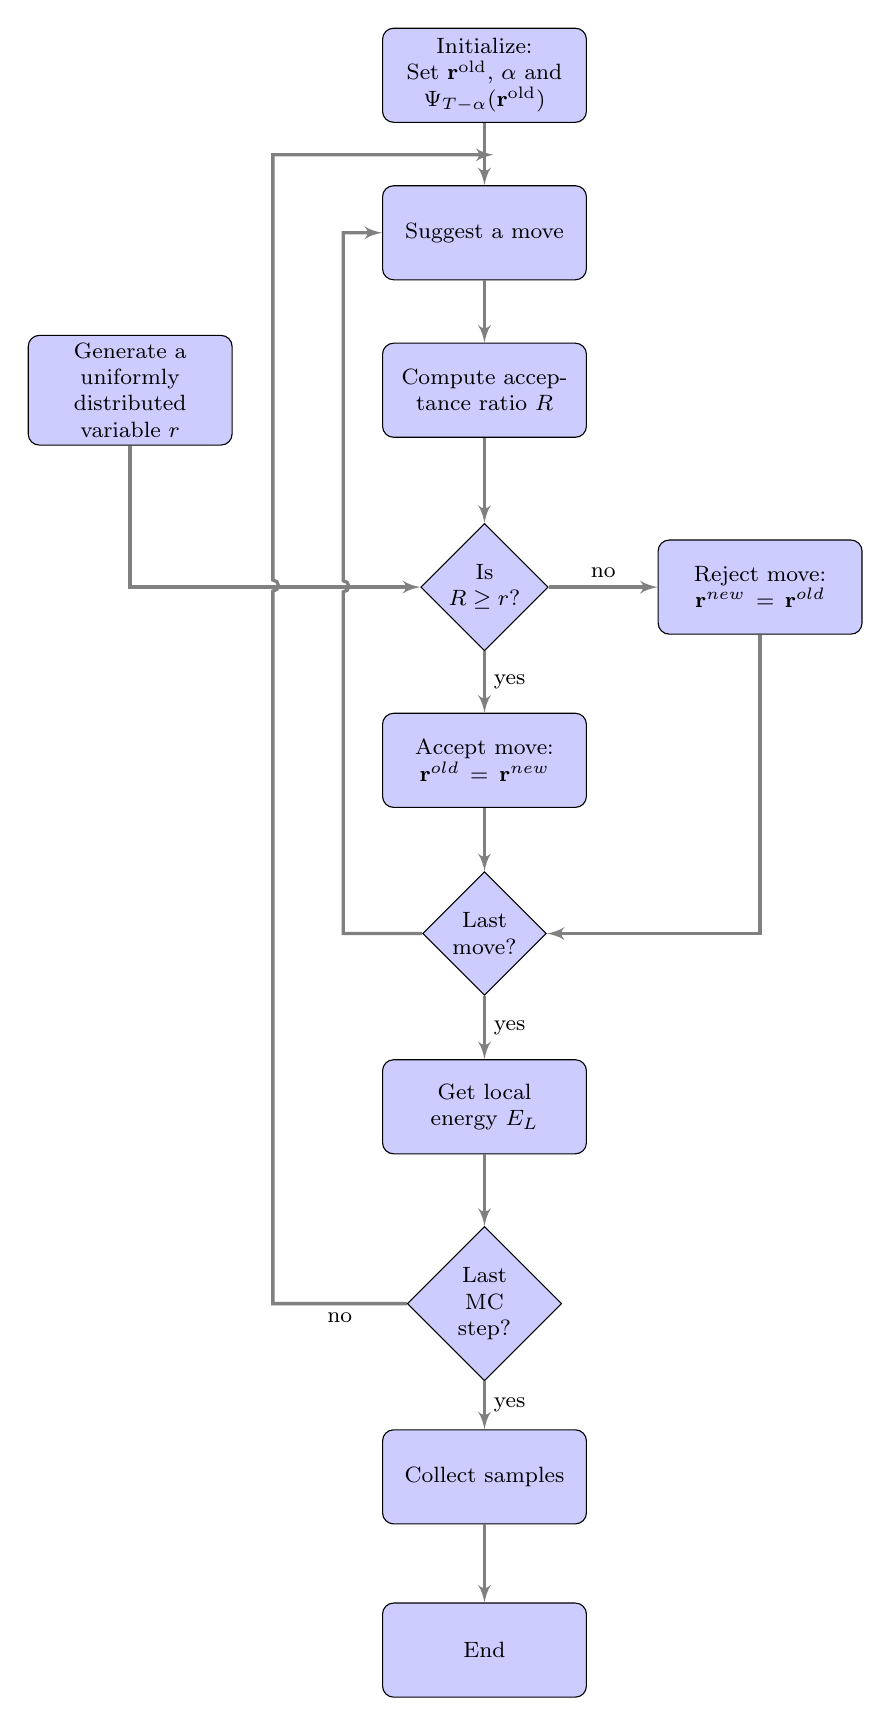
\begin{tikzpicture}[scale=1., node distance = 2cm, auto]
  \footnotesize
    % Place nodes
    \node [block] (init) {Initialize:\\
    Set ${\bf r}^{\mathrm{old}}$, $\alpha$ and $\Psi_{T-\alpha}({\bf r}^{\mathrm{old}})$};
    \node [block, below of=init, node distance=2.0cm] (suggestMove) {Suggest a move};
    \node [block, below of=suggestMove] (evaluateAcceptance) {Compute acceptance ratio $R$};
    \node [block, left of=evaluateAcceptance, node distance=4.5cm] (randomGenerator) {Generate a uniformly distributed variable $r$};
    \node [decision, below of=evaluateAcceptance] (decide) {Is\\ $R \geq r$?};
    \node [block, right of=decide, node distance=3.5 cm] (rejectMove) {Reject move: \\ ${\bf r}^{new} = {\bf r}^{old}$};
    \node [block, below of=decide, node distance=2.2cm] (acceptMove) {Accept move:\\${\bf r}^{old} = {\bf r}^{new}$};
    \node [decision, below of=acceptMove, node distance=2.2cm] (lastMove) {Last move?};
    \node [block, below of=lastMove, node distance=2.2cm] (getLocalEnergy) {Get local\\ energy $E_L$};
    \node [decision, below of=getLocalEnergy] (decideMC) {Last MC step?};
    \node [block, below of=decideMC, node distance=2.2cm] (collectSamples) {Collect samples};
    \node [block, below of=collectSamples, node distance=2.2cm] (end) {End};
    
%     % Draw edges
    \path [line] (init) -- (suggestMove);
    \path [line] (suggestMove) -- (evaluateAcceptance);
    \path [line] (evaluateAcceptance) -- (decide);
    \path [line] (randomGenerator) |- (decide);
    \path [line] (decide) -- node [, color=black] {yes}(acceptMove);
    \path [line] (decide) -- node [, color=black] {no}(rejectMove);
    \path [line] (acceptMove) -- (lastMove); 
    \path [line] (lastMove) -- node [, color=black] {yes}(getLocalEnergy);
    \path [line] (rejectMove) |- (lastMove);
    \path [line] (getLocalEnergy) -- (decideMC);
    \path [line] (decideMC) -- node [, color=black] {yes}(collectSamples);

    % Define a style for shifting a coordinate upwards
    % Note the curly brackets around the coordinate.
    \tikzstyle{s}=[shift={(0mm,\radius)}]
    \path[line] (lastMove.west) -- +(-1.0,0)  -- +(-1.0, 4.34) 
% % % %     % Draw semicircle junction to indicate that the lines are
% % % %     % not connected. Since we want the semicircle to have its center 
% % % %     % where the lines intersect, we have to shift the intersection 
% % % %     % coordinate using the 's' style to account for this.
    arc(-90:90:\radius) -- +(0.0, 4.42) -- (suggestMove.west);
    
    \path [line] (decideMC.west) -- node [, color=black]{no} +(-1.7,0) --+(-1.7,9.05) arc(-90:90:\radius) --+(0.0,5.4) -- +(2.8,5.4);
       
    \path [line] (collectSamples) -- (end);

\end{tikzpicture}\caption{Chart flow for the Quantum Varitional Monte Carlo algorithm.}\label{chartFlowMA}
\end{centering}
\end{figure}
The main part of the code contains calls to various functions, setup and 
declarations of arrays etc. 
Note that we have defined a fixed step length $h$ for the numerical computation of the second derivative 
of the kinetic energy. Furthermore, we perform the Metropolis test when we have moved all electrons.
This should be compared to the case where we move one electron at the time and perform the Metropolis test.
The latter is similar to the algorithm for the Ising model  discussed in the previous chapter.
A more detailed discussion and better statistical treatments and analyses are discussed in chapters
\ref{chap:advancedqmc} and \ref{chap:advancedatoms}. 
\begin{lstlisting}[title={\url{http://folk.uio.no/compphys/programs/chapter14/cpp/program1.cpp}}]
// Variational Monte Carlo for atoms with up to two electrons 
#include <iostream>
#include <fstream>
#include <iomanip>
#include "lib.h"
using namespace  std;
// output file as global variable
ofstream ofile;  
// the step length and its squared inverse for the second derivative 
#define h 0.001
#define h2 1000000

// declaraton of functions 

// Function to read in data from screen, note call by reference  
void initialise(int&, int&, int&, int&, int&, int&, double&) ;

// The Mc sampling for the variational Monte Carlo 
void  mc_sampling(int, int, int, int, int, int, double, double *, double *);

// The variational wave function 
double  wave_function(double **, double, int, int);

// The local energy 
double  local_energy(double **, double, double, int, int, int);

// prints to screen the results of the calculations  
void  output(int, int, int, double *, double *);


// Begin of main program   

//int main()
int main(int argc, char* argv[])
{
  char *outfilename;
  int number_cycles, max_variations, thermalization, charge;
  int dimension, number_particles; 
  double step_length;
  double *cumulative_e, *cumulative_e2;

  // Read in output file, abort if there are too few command-line arguments
  if( argc <= 1 ){
    cout << "Bad Usage: " << argv[0] << 
      " read also output file on same line" << endl;
    exit(1);
  }
  else{
    outfilename=argv[1];
  }
  ofile.open(outfilename); 
  //   Read in data 
  initialise(dimension, number_particles, charge, 
             max_variations, number_cycles, 
	     thermalization, step_length) ;
  cumulative_e = new double[max_variations+1];
  cumulative_e2 = new double[max_variations+1];
  
  //  Do the mc sampling  
  mc_sampling(dimension, number_particles, charge, 
              max_variations, thermalization, 
	      number_cycles, step_length, cumulative_e, cumulative_e2);
  // Print out results  
  output(max_variations, number_cycles, charge, cumulative_e, cumulative_e2);
  delete [] cumulative_e; delete [] cumulative_e; 
  ofile.close();  // close output file
  return 0;
}
\end{lstlisting}

The implementation of the brute force Metropolis algorithm is shown in the next function.
Here we have a loop over the variational variables $\alpha$. It calls two functions, one to compute the wave function
and one to update the local energy.
\begin{lstlisting}
// Monte Carlo sampling with the Metropolis algorithm  

void mc_sampling(int dimension, int number_particles, int charge, 
                 int max_variations, 
                 int thermalization, int number_cycles, double step_length, 
                 double *cumulative_e, double *cumulative_e2)
{
  int cycles, variate, accept, dim, i, j;
  long idum;
  double wfnew, wfold, alpha, energy, energy2, delta_e;
  double **r_old, **r_new;
  alpha = 0.5*charge;
  idum=-1;
  // allocate matrices which contain the position of the particles  
  r_old = (double **) matrix( number_particles, dimension, sizeof(double));
  r_new = (double **) matrix( number_particles, dimension, sizeof(double));
  for (i = 0; i < number_particles; i++) { 
    for ( j=0; j < dimension; j++) {
      r_old[i][j] = r_new[i][j] = 0;
    }
  }
  // loop over variational parameters  
  for (variate=1; variate <= max_variations; variate++){
    // initialisations of variational parameters and energies 
    alpha += 0.1;  
    energy = energy2 = 0; accept =0; delta_e=0;
    //  initial trial position, note calling with alpha 
    //  and in three dimensions 
    for (i = 0; i < number_particles; i++) { 
      for ( j=0; j < dimension; j++) {
	r_old[i][j] = step_length*(ran1(&idum)-0.5);
      }
    }
    wfold = wave_function(r_old, alpha, dimension, number_particles);
    // loop over monte carlo cycles 
    for (cycles = 1; cycles <= number_cycles+thermalization; cycles++){ 
      // new position 
      for (i = 0; i < number_particles; i++) { 
	for ( j=0; j < dimension; j++) {
	  r_new[i][j] = r_old[i][j]+step_length*(ran1(&idum)-0.5);
	}
      }
      wfnew = wave_function(r_new, alpha, dimension, number_particles); 
      // Metropolis test 
      if(ran1(&idum) <= wfnew*wfnew/wfold/wfold ) { 
	for (i = 0; i < number_particles; i++) { 
	  for ( j=0; j < dimension; j++) {
	    r_old[i][j]=r_new[i][j];
	  }
	}
	wfold = wfnew;
	accept = accept+1;
      }
      // compute local energy  
      if ( cycles > thermalization ) {
	delta_e = local_energy(r_old, alpha, wfold, dimension, 
                               number_particles, charge);
	// update energies  
        energy += delta_e;
        energy2 += delta_e*delta_e;
      }
    }   // end of loop over MC trials   
    cout << "variational parameter= " << alpha 
	 << " accepted steps= " << accept << endl;
    // update the energy average and its squared 
    cumulative_e[variate] = energy/number_cycles;
    cumulative_e2[variate] = energy2/number_cycles;
    
  }    // end of loop over variational  steps 
  free_matrix((void **) r_old); // free memory
  free_matrix((void **) r_new); // free memory
}   // end mc_sampling function  
\end{lstlisting}
The wave function is in turn defined in the next function.
Here we limit ourselves to   a function which consists only of 
the product of single-particle wave
functions.
\begin{lstlisting}
// Function to compute the squared wave function, simplest form 

double  wave_function(double **r, double alpha,int dimension, int number_particles)
{
  int i, j, k;
  double wf, argument, r_single_particle, r_12;
  
  argument = wf = 0;
  for (i = 0; i < number_particles; i++) { 
    r_single_particle = 0;
    for (j = 0; j < dimension; j++) { 
      r_single_particle  += r[i][j]*r[i][j];
    }
    argument += sqrt(r_single_particle);
  }
  wf = exp(-argument*alpha) ;
  return wf;
}
\end{lstlisting}
Finally, the local energy is computed using a numerical derivation for the kinetic 
energy.
We use the familiar expression derived in
Eq.~(\ref{eq:seconderivative}), that is
\[
 f_0''=\frac{ f_h -2f_0 +f_{-h}}{h^2},
\]
in order to compute 
\be 
  -\frac{1}{2\psi_T({\bf R})} \nabla^2\psi_T({\bf R}). 
\ee
The variable $h$ is a chosen step length. For helium, since it is
rather easy to evaluate the local energy, the above is an unnecessary
complication. However, for many-electron or other many-particle systems,
the derivation of a closed-form expression for the kinetic energy can be 
quite involved, and the numerical evaluation of the kinetic
energy using  Eq.~(\ref{eq:seconderivative}) may result in a simpler
code and/or even a faster one. 
\begin{lstlisting}
// Function to calculate the local energy with num derivative

double  local_energy(double **r, double alpha, double wfold, int dimension, 
                        int number_particles, int charge)
{
  int i, j , k;
  double e_local, wfminus, wfplus, e_kinetic, e_potential, r_12, 
    r_single_particle;
  double **r_plus, **r_minus;
  
  // allocate matrices which contain the position of the particles  
  // the function matrix is defined in the progam library 
  r_plus = (double **) matrix( number_particles, dimension, sizeof(double));
  r_minus = (double **) matrix( number_particles, dimension, sizeof(double));
  for (i = 0; i < number_particles; i++) { 
    for ( j=0; j < dimension; j++) {
      r_plus[i][j] = r_minus[i][j] = r[i][j];
    }
  }
  // compute the kinetic energy  
  e_kinetic = 0;
  for (i = 0; i < number_particles; i++) {
    for (j = 0; j < dimension; j++) { 
      r_plus[i][j] = r[i][j]+h;
      r_minus[i][j] = r[i][j]-h;
      wfminus = wave_function(r_minus, alpha, dimension, number_particles); 
      wfplus  = wave_function(r_plus, alpha, dimension, number_particles); 
      e_kinetic -= (wfminus+wfplus-2*wfold);
      r_plus[i][j] = r[i][j];
      r_minus[i][j] = r[i][j];
    }
  }
  // include electron mass and hbar squared and divide by wave function 
  e_kinetic = 0.5*h2*e_kinetic/wfold;
  // compute the potential energy 
  e_potential = 0;
  // contribution from electron-proton potential  
  for (i = 0; i < number_particles; i++) { 
    r_single_particle = 0;
    for (j = 0; j < dimension; j++) { 
      r_single_particle += r[i][j]*r[i][j];
    }
    e_potential -= charge/sqrt(r_single_particle);
  }
  // contribution from electron-electron potential  
  for (i = 0; i < number_particles-1; i++) { 
    for (j = i+1; j < number_particles; j++) {
      r_12 = 0;  
      for (k = 0; k < dimension; k++) { 
	r_12 += (r[i][k]-r[j][k])*(r[i][k]-r[j][k]);
      }
      e_potential += 1/sqrt(r_12);          
    }
  }
  free_matrix((void **) r_plus); // free memory
  free_matrix((void **) r_minus);
  e_local = e_potential+e_kinetic;
  return e_local;
}
\end{lstlisting}
The remaining part of the program consists of the output and initialize functions and is not listed here. 


The way we have rewritten Schr\"odinger's equation results in energies
given in atomic units. If we wish to convert these energies into more familiar
units like electronvolt (eV), we have to multiply our reults with
$2E_0$ where $E_0=13.6$ eV, the binding energy of the hydrogen atom.
Using Eq.~(\ref{eq:wavehelium1}) for the trial wave function, we obtain an
energy minimum at  $\alpha =1.6875$\footnote{With hydrogen like wave functions for the 
$1s$ state one can easily calculate the energy of the ground state for the helium atom as function of the charge $Z$. The results is $E[Z]= Z^2-4Z+\frac{5}{8}Z$, and taking the derivative with respect to $Z$ to find the minumum
we get $   Z=2-\frac{5}{16} = 1.6875$. This number represents an optimal effective charge.}.
The ground state is 
$E=-2.85$ in atomic units or $E=-77.5$ eV. The experimental value is
$-78.8$ eV. Obviously, improvements to the wave function such as 
including the 'cusp'-condition for the two electrons as well, see
Eq.~(\ref{eq:wavehelium2}), could improve our agreement with experiment.

We note that the effective charge is less than the charge of the nucleus.
We can interpret this reduction as an effective way of incorporating
the repulsive electron-electron interaction.
Finally, since we do not have the exact wave function, we see from
Fig.~\ref{fig:sigmahelium} that the variance is not zero at the energy 
minimum. 
\begin{figure}
\begin{center}
\input{figures/sigmahelium}
\end{center}
\caption{Result for ground state energy of the helium atom using
         Eq.~(\ref{eq:wavehelium1}) for the trial wave function. 
         A total of $10^7$ Monte Carlo moves were used
         with a step length of 1 Bohr radius. Approximately 50\% of all proposed moves were accepted.
The variance at the minimum is 1.026, reflecting the fact that we do not have the exact wave function. The variance has a minimum at value of $\alpha$ different from the energy minimum. The numerical results are compared with 
the exact result $E[Z]= Z^2-4Z+\frac{5}{8}Z$.\label{fig:sigmahelium}}
\end{figure}
Techniques such as importance sampling, to be contrasted to the brute force Metropolis sampling 
used here,
and various optimization techniques of the variance and the energy, will be discussed in the next section and in 
chapter \ref{chap:advancedqmc}.

\subsection{Importance sampling}


As mentioned in connection with the generation of random numbers, sequential correlations must be
given thorough attention as it may lead to bad error estimates of our
numerical results.

There are several things we need to keep in mind in order to keep the
correlation low. First of all, the transition acceptance must be kept
as high as possible. Otherwise, a walker will dwell at the same spot
in state space for several iterations at a time, which will clearly
lead to high correlation between nearby succeeding measurements.

Secondly, when using the simple symmetric form of $\omega(\vec
r_\textrm{old}\textrm{, }\vec r_\textrm{new})$, one has to keep in
mind the random walk nature of the algorithm. Transitions will be made
between points that are relatively close to each other in state space,
which also clearly contributes to increase correlation. The
seemingly obvious way to deal with this would be just to
increase the step size, allowing the walkers to cover more of the
state space in fewer steps (thus requiring fewer steps to reach
ergodicity). But unfortunately, long before the step length becomes
desirably large, the algorithm breaks down. When proposing moves
symmetrically and uniformly around $\vec r_\textrm{old}$, the step
acceptance becomes directly dependent on the step length in such a way
that a too large step length reduces the acceptance. The reason for
this is very simple. As the step length increases, a walker will more
likely be given a move proposition to areas of very low probability,
particularly if the governing trial wave function describes a
localized system. In effect, the effective movement of the
walkers again becomes too small, resulting in large correlation. For
optimal results we therefore have to balance the step length with the
acceptance.

With a transition suggestion rule $\omega$ as simple as the uniform
symmetrical one emphasized so far, the usual rule of thumb is to keep
the acceptance around $0.5$. But the optimal interval varies a
lot from case to case. We therefore have to treat each numerical
experiment with care.

By choosing a better $\omega$, we can still improve the efficiency of
the step length versus acceptance. Recall that $\omega$ may be chosen
arbitrarily as long as it fulfills ergodicity, meaning that it has to
allow the walker to reach any point of the state space in a finite
number of steps. What we basically want is an $\omega$ that pushes the
ratio towards unity,
increasing the acceptance. The theoretical situation of $\omega$
exactly equal to $p$ itself:
\bdm
\omega(\vec r_\textrm{new}\textrm{, }\vec r_\textrm{old})=
\omega(\vec r_\textrm{new}) = p(\vec r_\textrm{new})
\edm
would give the maximal acceptance of $1$. But then we would already
have solved the problem of producing points distributed according to
$p$. One typically settles on modifying the symmetrical $\omega$ so
that the walkers move more towards areas of the state space where the
distribution is large. One such procedure is the Fokker-Planck
formalism where the walkers are moved according to
the gradient of the distribution. The formalism ``pushes'' the walkers
in a ``desirable'' direction. The idea is to propose moves similarly
to an isotropic diffusion process with a drift. A new position $\vec
x_\textrm{new}$ is calculated from the old one, $\vec x_\textrm{old}$,
as follows:
\be
\vec r_\textrm{new} = \vec r_\textrm{old} + \chi +
D\vec F(\vec r_\textrm{old})\delta t
\label{eq:drift_diffusion_proposition}
\ee
Here $\chi$ is a Gaussian pseudo-random number with mean equal zero
and variance equal $2D\delta t$. It accounts for the diffusion part of
the transition. The third term on the left hand side accounts for the
drift. $\vec F$ is a drift velocity dependent on the position of the
walker and is derived from the quantum mechanical wave function
$\psi$. The constant $D$, being the diffusion constant of $\chi$, also
adjusts the size of the drift. $\delta t$ is a time step parameter
whose presence will be clarified shortly.

It can be shown that the $\omega$ corresponding to
the move proposition rule in Eq.~(\ref{eq:drift_diffusion_proposition})
becomes (in non-normalized form):
\be
\omega(\vec r_\textrm{old}\textrm{, }\vec r_\textrm{new}) =
\exp\left(
-\frac{(\vec r_\textrm{new}-\vec r_\textrm{old}-D\delta t\vec F(\vec
  r_\textrm{old}))^2}{4D\delta t}\right)
\label{eq:omega_drift_diffusion}
\ee
which, as expected, is a Gaussian with variance $2D\delta t$ centered
slightly off $\vec r_\textrm{old}$ due to the drift term $D\vec F(\vec
r_\textrm{old})\delta t$.

What is the optimal choice for the drift term? From statistical
mechanics we know that a simple isotropic drift diffusion process
obeys a Fokker-Planck equation of the form:
\be
\frac{\partial f}{\partial t} = \sum_i D \frac{\partial}{\partial x_i}
\left(\frac{\partial}{\partial x_i}-F_i(\vec F)\right)f
\label{eq:fokker-planck}
\ee
where $f$ is the continuous distribution of walkers.
Equation (\ref{eq:drift_diffusion_proposition}) is a discretized realization
of such a process where $\delta t$ is the discretized time step. In
order for the solution $f$ to converge to the desired distribution
$p$, it can be shown that the drift velocity has to
be chosen as follows:
\bdm
\vec F = \frac{1}{f}\vec\nabla f
\edm
where the operator $\vec\nabla$ is the vector of first derivatives of
all spatial coordinates. Convergence for such a diffusion process is
only guaranteed when the time step approaches zero. But in the
Metropolis algorithm, where drift diffusion is used just as a
transition proposition rule, this bias is corrected automatically by
the rejection mechanism. In our application, the desired probability distribution function  being the
square absolute of the wave function, $f = |\psi|^2$, the drift
velocity becomes:
\be
\vec F = 2\frac{1}{\psi}\vec\nabla\psi
\label{eq:drift_velocity_VMC}
\ee
As expected, the walker is ``pushed'' along the gradient of the wave
function.

When dealing with many-particle systems, 
we should also consider whether to move only one
particle at a time at each transition or all at once. The former
method may often be more efficient. A movement of only one particle
will restrict the accessible space a walker can move to in a single
transition even more, thus introducing correlation. But on the other
hand, the acceptance is increased so that each particle can be moved
further than it could in a standard all-particle move. It is also
computationally far more efficient to do one-particle transitions
particularly when dealing with complicated distributions governing
many-dimensional anti-symmetrical fermionic systems.

Alternatively, we can treat the sequence of all one-particle
transitions as one total transition of all particles. This gives a
larger effective step length thus reducing the correlation. From a
computational point of view, we may not gain any speed by summing up the
individual one-particle transitions as opposed to doing an
all-particle transition. But the reduced correlation increases the
total efficiency. We are able to do fewer calculations in order to
reach the same numerical accuracy.

%Then the block averages themselves become ergodic.
%It takes a correlation time for the walk to become ergodic.

Another way to acquire some control over the correlation is to do a so
called blocking procedure 
on our set of numerical measurements.  This is discussed in chapter \ref{chap:improvedvmc}.


\section{Exercises}

%\subsection*{Project 14.1: Studies of light Atoms}
\begin{prob}
The aim of this problem is to test the variational Monte Carlo apppled to light atoms.
We will test different trial wave function
$\Psi_T$.
The systems we study are atoms consisting of two electrons only, such as
the helium atom, Li$_{II}$ and  Be$_{III}$. The atom Li$_{II}$
has two electrons and 
$Z=3$ while Be$_{III}$  has $Z=4$ but still two electrons only.
A general ansatz for the trial wave function is
\be
   \psi_T({\bf R})=\phi({\bf r}_1)\phi({\bf r}_2)f(r_{12}).
\ee
For all systems we assume that the one-electron wave functions
$\phi({\bf r}_i)$ are described by the an elecron in the lowest 
hydrogen orbital $1s$.

The specific trial functions we study are
\be
   \psi_{T1}({\bf r_1},{\bf r_2}, {\bf r_{12}}) =
   \exp{\left(-\alpha(r_1+r_2)\right)},
\ee
where $\alpha$ is the variational parameter,
\be
   \psi_{T2}({\bf r_1},{\bf r_2}, {\bf r_{12}}) =
   \exp{\left(-\alpha(r_1+r_2)\right)}(1+\beta r_{12}),
\ee
with  $\beta$ as a new variational parameter and
\be
   \psi_{T3}({\bf r_1},{\bf r_2}, {\bf r_{12}}) =
   \exp{\left(-\alpha(r_1+r_2)\right)}
   \exp{\left(\frac{r_{12}}{2(1+\beta r_{12})}\right)}.
\ee

\begin{enumerate}
\item[a)] Find the closed-form  expressions for the local energy for the above trial wave function
for the helium atom. Study the behavior of the local energy with these functions in the limits 
$r_1\rightarrow 0$, 
$r_2\rightarrow 0$ and $r_{12}\rightarrow 0$.
\item[b)] Compute 
\be
   \langle \OP{H} \rangle =
   \frac{\int d{\bf R}\Psi^{\ast}_T({\bf R})\OP{H}({\bf R})\Psi_T({\bf R})}
        {\int d{\bf R}\Psi^{\ast}_T({\bf R})\Psi_T({\bf R})},
\ee
for the helium atom using the variational Monte Carlo method employing the 
Metropolis algorithm to sample the different states using the trial wave function
$\psi_{T1}({\bf r_1},{\bf r_2}, {\bf r_{12}})$. Compare your results with the closed-form expression 
\be
\langle\OP{H} \rangle = \frac{\hbar^2}{m_e} \alpha^2
		  - \frac{27}{32} \frac{e^2}{\pi \epsilon_0} \alpha.
\ee
\item[c)] 
Use the optimal value of $\alpha$ from the previous point to compute the ground state of the helium
atom using the other two trial wave functions
$\psi_{T2}({\bf r_1},{\bf r_2}, {\bf r_{12}})$ and
$\psi_{T3}({\bf r_1},{\bf r_2}, {\bf r_{12}})$. 
In this case you have to vary both $\alpha$ and $\beta$.
Explain briefly which function 
$\psi_{T1}({\bf r_1},{\bf r_2}, {\bf r_{12}})$,
$\psi_{T2}({\bf r_1},{\bf r_2}, {\bf r_{12}})$ and $\psi_{T3}({\bf r_1},{\bf r_2}, {\bf r_{12}})$ is
the best.
\item[d)]
Use the optimal value for all parameters and all wave functions to compute 
the expectation value of the mean distance $\langle r_{12} \rangle$
between the two electrons. Comment your results.
\item[e)] We will now repeat point 1c), but we replace the helium atom with the ions
Li$_{II}$ and Be$_{III}$. 
Perform first a variational calculation using the first ansatz for the trial wave function
$\psi_{T1}({\bf r_1},{\bf r_2}, {\bf r_{12}})$ in order to find an optimal value for
$\alpha$. Use then this value to start the variational calculation of the energy for the wave 
functions
$\psi_{T2}({\bf r_1},{\bf r_2}, {\bf r_{12}})$
and $\psi_{T3}({\bf r_1},{\bf r_2}, {\bf r_{12}})$.
Comment your results.
\end{enumerate}
\end{prob}

%\subsection*{Project 14.2: The H$_2^+$ molecule}
\begin{prob}
The H$_2^+$ molecule  consists of  two protons and one electron,
with binding energy  $E_B=-2.8$ eV
and an equilibrium position  $r_0=0.106$ nm between the 
two protons.

We define our system through the following variables.
The electron is at a distance 
${\bf r}$ from a chosen origo, 
one of the protons is at the distance 
$-{\bf R}/2$ while the other one is placed at
${\bf R}/2$ from origo, resulting
in a distance to the electron of 
${\bf r}- {\bf R}/2$ and ${\bf r}+ {\bf R}/2$, respectively.

In our solution of Schr\"odinger's equation for this system we are going
to neglect the kinetic energies of the protons, since they are
2000 times heavier than the electron. We assume thus that their
velocities are negligible compared to the velocity of the electron.
In addition we omit contributions from  nuclear forces, since they act
at distances of several orders of magnitude smaller than the 
equilibrium position. 
 
We can then write Schr\"odinger's equation as follows
\be
    \left\{-\frac{\hbar^2\nabla_r^2}{2m_e}
     -\frac{ke^2}{|{\bf r}- {\bf R}/2|}-\frac{ke^2}{|{\bf r}+ {\bf R}/2|}
     +\frac{ke^2}{R}
     \right\}\psi({\bf r},{\bf R})=E\psi({\bf r},{\bf R}),
\ee
where the first term is the kinetic energy of the electron,
the second term is the potential energy the electron feels
from the proton at 
$-{\bf R}/2$  while the third term arises from the potential
energy contribution from the proton at 
${\bf R}/2$. 
The last term arises due to the repulsion between the two protons.


Since the potential is symmetric with respect to the interchange 
of 
${\bf R}\rightarrow -{\bf R}$
and  ${\bf r}\rightarrow -{\bf r}$
it means that the probability for the electron to move from one 
proton to the other must be equal in both directions.
We can say that the electron shares it's time between both
protons.

With this caveat, we can now construct a model for simulating this
molecule.
Since we have only one elctron, we could assume that in the limit 
$R\rightarrow
\infty$, i.e., when the distance between the two protons is large,
the electron is essentially bound to only one of the protons.
This should correspond to a hydrogen atom. 
As a trial wave function, we could therefore use the electronic wave function
for the ground  state of hydrogen, namely
\be
    \psi_{100}(r)=\left(\frac{1}{\pi a_0^3}\right)^{1/2} e^{-r/a_0}.
\ee
Since we do not know exactly where the electron is, we have to allow
for the possibility that the electron can be coupled to one of the two
protons. This form includes the 'cusp'-condition discussed
in the previous section.
We define thence two 
hydrogen wave functions
\be
   \psi_1({\bf r},{\bf R})=\left(\frac{1}{\pi a_0^3}\right)^{1/2} e^{-|{\bf r}- {\bf R}/2|/a_0},
\ee
and
\be
   \psi_2({\bf r},{\bf R})=\left(\frac{1}{\pi a_0^3}\right)^{1/2} e^{-|{\bf r}+ {\bf R}/2|/a_0}.
\ee
Based on these two wave functions, which represent where the electron can be,
we attempt at the following  linear combination
\be
   \psi_{\pm}({\bf r},{\bf R})=C_{\pm}\left(\psi_1({\bf r},{\bf R})\pm\psi_2({\bf r},{\bf R})\right),
\ee
with $C_{\pm}$ a constant. 
Based on this discussion, 
we add a second electron in order to simulate the H$_2$ molecule. That is the topic for project 14.3.
\end{prob}


%\subsection*{Project 14.3: the H$_2$ molecule}

\begin{prob}
The 
H$_2$ molecule consists of two protons and two electrons 
with a ground state energy $E=-1.17460$ a.u. and equilibrium distance between the two hydrogen atoms
of $r_0=1.40$ Bohr radii.
We define our systems using the following variables.
Origo is chosen to be halfway between the two protons. The distance from 
proton 1 is defined as 
$-{\bf R}/2$ whereas proton 2 has a distance ${\bf R}/2$.
Calculations are performed for fixed distances ${\bf R}$ between the two protons.

Electron 1 has a distance $r_1$ from the chose origo, while  electron $2$
has a distance $r_2$. 
The kinetic energy operator becomes then
\be
   -\frac{\nabla_1^2}{2}-\frac{\nabla_2^2}{2}.
\ee
The distance between the two electrons is
$r_{12}=|{\bf r}_1-{\bf r}_2|$. 
The repulsion between the two electrons results in a potential energy term given by
\be
               +\frac{1}{r_{12}}.
\ee
In a similar way we obtain a repulsive contribution from the interaction between the two 
protons given by
\be
               +\frac{1}{|{\bf R}|},
\ee
where ${\bf R}$ is the distance between the two protons.
To obtain the final potential energy we need to include the attraction the electrons feel from the protons.
To model this, we need to define the distance between the electrons and the two protons.
If we model this along a 
chosen $z$-akse with electron 1 placed at a distance 
${\bf r}_1$ from a chose origo, one proton at $-{\bf R}/2$
and the other at  ${\bf R}/2$, 
the distance from proton 1 to electron 1 becomes
\be
{\bf r}_{1p1}={\bf r}_1+ {\bf R}/2,
\ee
and
\be
{\bf r}_{1p2}={\bf r}_1- {\bf R}/2,
\ee
from proton 2.
Similarly, for electron 2 we obtain
\be
{\bf r}_{2p1}={\bf r}_2+{\bf R}/2,
\ee
and
\be
{\bf r}_{2p2}={\bf r}_2-{\bf R}/2.
\ee
These four distances define the attractive contributions to the potential energy
\be
   -\frac{1}{r_{1p1}}-\frac{1}{r_{1p2}}-\frac{1}{r_{2p1}}-\frac{1}{r_{2p2}}.
\ee
We can then write the total Hamiltonian as 
\be
   \OP{H}=-\frac{\nabla_1^2}{2}-\frac{\nabla_2^2}{2}
   -\frac{1}{r_{1p1}}-\frac{1}{r_{1p2}}-\frac{1}{r_{2p1}}-\frac{1}{r_{2p2}}
               +\frac{1}{r_{12}}+\frac{1}{|{\bf R}|},
\ee
and if we choose ${\bf R}=0$ we obtain the helium atom.

In this project we will use a trial wave function of the form
\be
   \psi_{T}({\bf r_1},{\bf r_2}, {\bf R}) =
   \psi({\bf r}_1,{\bf R})\psi({\bf r}_2,{\bf R})
   \exp{\left(\frac{r_{12}}{2(1+\beta r_{12})}\right)},
\ee
with the following trial wave function 
\be
   \psi({\bf r}_1,{\bf R})=\left(\exp{(-\alpha r_{1p1})}
      +\exp{(-\alpha r_{1p2})}\right),
\ee
for electron 1 and
\be
   \psi({\bf r}_2,{\bf R})=\left(\exp{(-\alpha r_{2p1})}
      +\exp{(-\alpha r_{2p2})}\right).
\ee
The variational parameters are $\alpha$ and $\beta$.

One can show that in the limit where all distances approach zero that 
\be
    \alpha = 1+\exp{(-R/\alpha)},
    \label{eq:alpha}
\ee
resulting in $\beta$ kas the only variational parameter.
The last equation is a non-linear equation which we can solve with for example
Newton's method discussed in chapter \ref{chap:nonlinear}.
\begin{enumerate}
\item Find the local energy as function of 
$R$.
\item Set up and algorithm and write a program which computes the 
expectation value of 
$\langle \OP{H} \rangle$
using the variational Monte Carlo method with a brute force Metropolis sampling.
For each inter-proton distance  $R$ you must find the parameter 
$\beta$ which minimizes the energy. Plot the corresponding energy as function
of the distance $R$ between the protons.
\item Use thereafter the optimal parameter sets to compute the 
average distance
$\langle r_{12} \rangle$ between the electrons where the energy as function of
$R$ exhibits its minimum. Comment your results.
\item 
We modify now the approximation for the wave functions of electrons 1 and 2
by subtracting the two terms instead of adding up, viz
\be
   \psi({\bf r}_1,{\bf R})=\left(\exp{(-\alpha r_{1p1})}
      -\exp{(-\alpha r_{1p2})}\right),
\ee
for electron 1 
\be
   \psi({\bf r}_2,{\bf R})=\left(\exp{(-\alpha r_{2p1})}
      -\exp{(-\alpha r_{2p2})}\right),
\ee
for electron 2. Mathematically, this approach is equally viable as the previous one.
Repeat your calculations from point b) and see if you can obtain an energy minimum as 
function of  $R$. Comment your results.
\end{enumerate}
\end{prob}








%%%%%%%%%%%%%%%%%%%%%part.tex%%%%%%%%%%%%%%%%%%%%%%%%%%%%%%%%%%
% 
% sample part title
%
% Use this file as a template for your own input.
%
%%%%%%%%%%%%%%%%%%%%%%%% Springer %%%%%%%%%%%%%%%%%%%%%%%%%%

\begin{partbacktext}
\part{Advanced topics}
The last part of this book contains several project oriented advanced topics.
Each of these topics can serve as a regular one-semester course based on the 
solution of the pertinent projects.  We present several topics, mainly within
applications to quantum mechanical systems and statistical mechanics. 
We discuss Hartree-Fock and density-functional theory 
calculations for electronic systems, variational
and diffusion Monte Carlo calculations of many-particle systems
(atoms, quantum dots and Bose-Einstein condensation), large molecular-dynamics
calculations of solids, percolation and critical phenomena and advanced
simulations of phase transitions.
\end{partbacktext}

 \clearemptydoublepage
\chapter{Many-body approaches to studies of electronic systems: Hartree-Fock theory and Density Functional Theory}\label{chap:advancedatoms}

\abstract{This chapter presents the Hartree-Fock method with an emphasis on computing
the energies of selected closed-shell atoms.}
\section{Introduction}
A theoretical understanding of the behavior of quantum mechanical systems  
with many interacting particles, normally called
many-body systems,  
is a  great challenge and provides fundamental insights into systems governed by quantum mechanics, as well 
as offering potential areas of industrial applications, from semi-conductor physics  to the construction of quantum 
gates.  
The capability to simulate quantum mechanical systems with many interacting particles is crucial for advances
in such rapidly developing fields like materials science.

However, 
most  quantum mechanical systems of interest in  physics consist of a large number of
interacting particles.
The total number of particles $N$ is usually sufficiently large
that an exact solution (viz., in closed form) cannot be found.  One needs therefore reliable numerical methods
for studying quantum mechanical systems with many particles.


Studies of many-body systems
span from our understanding of the strong force with quarks and 
gluons as degrees of freedom, the spectacular macroscopic manifestations of quantal phenomena such as
Bose-Einstein condensation with millions of atoms forming a coherent state,  to properties of new materials, with 
electrons as effective degrees of freedom. The length scales range from few micrometers and nanometers, typical scales met in materials science, 
to $10^{-15}-10^{-18}$ m,
a relevant length scale  for the strong interaction. Energies can span from few meV to GeV or even TeV. 
In some cases the basic interaction between the interacting particles is well-known. 
A good example is the
Coulomb force, familiar from studies of atoms, molecules and condensed matter physics. 
In other cases, such as for the strong interaction
between neutrons and protons (commonly dubbed as nucleons) or dense quantum liquids 
one has to resort to parameterizations of the underlying interparticle 
interactions. 
But the system can also span over much larger dimensions as well, with neutron stars as one of the classical objects.
This star is the endpoint of massive stars which have used up their fuel.
A neutron star, as its name suggests, is composed mainly of neutrons, with a small fraction of protons and 
probably quarks in its inner parts.  The star is extremely dense and compact, with a radius of approximately 
10 km and a mass which is roughly $1.5$ times that of our sun. The quantum mechanical pressure which is set up by the
interacting particles counteracts the gravitational forces, hindering thus a gravitational collapse.
To describe a neutron star one needs to solve Schr\"odinger's equation for approximately $10^{54}$ 
interacting particles! 

With a given interparticle potential and the kinetic energy of the system, 
one can in turn define the so-called
many-particle Hamiltonian $\hat{H}$ which enters the solution of Schr\"odinger's equation or Dirac's equation in case relativistic effects
need to be included.   
For many particles, Schr\"odinger's equation is an integro-differential equation whose complexity increases exponentially
with increasing numbers of particles and states that the system can access.  
Unfortunately, apart from some few analytically solvable problems and one and two-particle systems that can be treated
numerically exactly  
via the solution of sets of partial differential equations,  
the typical absence of an exactly solvable (on closed form) contribution to the many-particle Hamiltonian 
means that we need reliable numerical many-body methods. 
These methods should allow for controlled approximations
and provide a computational scheme which accounts for successive 
many-body corrections in a systematic way.  

Typical examples of 
popular many-body methods are coupled-cluster methods 
\cite{kummel1978,bartlett2007,helgaker,dean2004,Kowalski2004}, 
various types of 
Monte Carlo methods \cite{Pudliner1997,kdl1997,ceperley1995}, 
perturbative many-body methods \cite{ellis1977,lindgren,hko1995}, 
Green's function methods \cite{dickhoff,blaizot},  
the density-matrix renormalization group \cite{white1992,schollwock2005}, density functional theory \cite{jones1989} and 
ab initio density functional theory \cite{bartlett2005,peirs2003,vanneck2006}, and large-scale diagonalization methods 
\cite{Whitehead1977,caurier2005,horoi2006}, just to mention a few. 
The physics of the system hints at which many-body methods to use. For systems with strong correlations
among the constituents, methods based on mean-field theory such as Hartree-Fock theory and density functional theory are normally ruled out.
This applies also to perturbative methods, unless one can renormalize the parts of the interaction which cause problems.

The aim of this and the next three chapters is to present to you many-body methods
which can be used to study properties of atoms, molecules, systems in the solid state 
and nuclear physics. We limit the attention to non-relativistic quantum mechanics.

In this chapter
we limit ourselves to studies of electronic systems such atoms, molecules and quantum dots, 
as discussed partly in chapter \ref{chap:mcvar} as well.
Using the Born-Oppenheimer approximation we rewrote Schr\"odinger's equation for $N$ electrons as 
\[
  \left[-\sum_{i=1}^N \frac{1}{2} \nabla^2_i 
    - \sum_{i=1}^N \frac{Z}{r_i} + \sum_{i<j}^N \frac{1}{r_{ij}} 
    \right] \Psi(\mathbf{R}) = E \Psi(\mathbf{R}), 
\]
where we let $\mathbf{R}$ represent the positions which the $N$ electrons can take, that is $\mathbf{R}=\left\{\mathbf{r}_1,\mathbf{r}_2,\dots,\mathbf{r}_N\right\}$. 
With more than one electron present we cannot find an solution on a closed form and must resort to numerical efforts. In this
chapter we will examine Hartree-Fock theory 
applied to the atomic problem. However, the machinery we expose can easily be extended to studies of molecules or two-dimensional systems like quantum dots.

For atoms and molecules, the electron-electron interaction 
is rather weak compared with the attraction from the nucleus. An independent particle picture
is therefore a viable first step towards the solution of Schr\"odinger's equation. 
We assume therefore that each electrons sees an effective field set up by the other electrons.
This leads to an integro-differential equation  and methods like Hartree-Fock theory discussed in this chapter.


In practical terms, for the Hartree-Fock method we end up solving a one-particle equation, as is the case for the hydrogen atom but modified due 
to the screening from the other electrons.  This modified single-particle equation reads (see Eq.~(\ref{eq:radialsl} for the hydrogen case)
in atomic units
\[
  -\frac{1}{2} \frac{d^2}{dr^2} u_{nl}(r) 
       + \left (\frac{l (l + 1)}{2r^2}-\frac{Z}{r}+ \Phi(r)+F_{nl}\right ) u_{nl}(r)  = e_{nl} u_{nl}(r) .
\]
The function $u_{nl}$ is the solution of the radial part of the Schr\"odinger equation and the functions $\Phi(r)$ and
$F_{nl}$ are the corrections due to the screening from the other electrons.  We will derive these equations in the next section.

The total one-particle wave function, see chapter \ref{chap:mcvar}  is 
\[
  \psi_{nlm_lsm_s} = \phi_{nlm_l}({\bf r})\xi_{m_s}(s)
\]
with $s$ is the spin ($1/2$ for electrons), $m_s$ is the spin projection $m_s=\pm 1/2$, and the spatial part is
\[
   \phi_{nlm_l}({\bf r}) =  R_{nl}(r)Y_{lm_l}(\hat{{\bf r}})
\]
with $Y$ the spherical harmonics discussed in chapter \ref{chap:mcvar} and $u_{nl} = rR_{nl}$.
The other quantum numbers are the orbital momentum  $l$ and its projection $m_l=-l,-l+1,\dots,l-1,l$ and the principal quantum
number $n=n_r+l+1$, with $n_r$ the number of nodes of a given single-particle wave function. 
All results are in atomic units, meaning that the energy is given by $e_{nl}=-Z^2/2n^2$ and the radius is dimensionless.


We obtain then a modified single-particle eigenfunction which in turn can be used
as an input in a variational Monte Carlo calculation of the ground state of a specific atom. 
This is the aim of the next chapter. Since Hartree-Fock theory does not treat 
correctly the role of many-body correlations, the hope is that
performing a Monte Carlo calculation we may improve our results by obtaining a better agreement with experiment.

In the next chapter we focus 
on the variational Monte Carlo method as a way to improve upon the Hartree-Fock results.  
Although the variational Monte Carlo approach will improve our agreement with experiment compared with the Hartree-Fock results, there are still further possibilities
for improvement. This is provided by Green's function Monte Carlo methods, which allow for an in principle exact calculation.
The diffusion Monte Carlo method is discussed in chapter 
\ref{chap:advancedqmc}, with an application to studies of Bose-Einstein condensation.
Other many-body methods such as large-scale diagonalization and coupled-cluster theories are 
discussed in Ref.~\cite{deanhj2009}.






\section{Hartree-Fock theory}\label{sec:hf}


Hartree-Fock theory \cite{helgaker,bransden1983}
is one of the simplest approximate theories  
for solving the many-body Hamiltonian. It is based on a simple
approximation to the true many-body wave-function; that the
wave-function is given by a single Slater determinant of $N$ 
orthonormal single-particle wave functions\footnote{We limit ourselves to a restricted 
Hartree-Fock approach and assume that all the lowest-lying orbits are filled. This constitutes 
an approach suitable for systems with filled shells. 
The theory we outline is therefore applicable to systems which 
exhibit so-called magic numbers like the noble gases, closed-shell nuclei  
like $^{16}$O and $^{40}$Ca and quantum dots with magic number fillings.}
\[
  \psi_{nlm_lsm_s} = \phi_{nlm_l}({\bf r})\xi_{m_s}(s).
\]
We use hereafter the shorthand $\psi_{nlm_lsm_s}({\bf r}) = \psi_{\alpha}({\bf r})$,
where $\alpha$ now contains all the quantum numbers  needed to specify a particular single-particle orbital.

The Slater determinant can then be written as   
\begin{equation}
  \Phi(\mathbf{r}_1,\mathbf{r}_2,\dots,\mathbf{r}_N,\alpha,\beta,\dots,\nu)  = \frac{1}{\sqrt{N!}}\left| 
  \begin{array}{cccc}
    \psi_{\alpha}(\mathbf{r}_1)&\psi_{\alpha}(\mathbf{r}_2)&\dots&\psi_{\alpha}(\mathbf{r}_N) \\ [4pt]
    \psi_{\beta}(\mathbf{r}_1)&\psi_{\beta}(\mathbf{r}_2)&\dots&\psi_{\beta}(\mathbf{r}_N) \\[4pt] 
    \vdots              & \vdots            &\ddots&\vdots\\[4pt]
    \psi_{\nu}(\mathbf{r}_1)&\psi_{\beta}(\mathbf{r}_2)&\dots&\psi_{\beta}(\mathbf{r}_N)
  \end{array}
  \right|.
\label{HartreeFockDet}
\end{equation}
Here the variables $\mathbf{r}_i$ include the coordinates of 
spin and space of particle $i$. The quantum numbers $\alpha,\beta,\dots,\nu$ encompass all possible quantum numbers needed to specify a 
particular system. As an example, consider the Neon atom, with ten electrons which can fill the $1s$, $2s$ and $2p$ single-particle
orbitals. Due to the spin projections $m_s$ and orbital momentum projections $m_l$, the $1s$ and $2s$ states have  a degeneracy of $2(2l+1)=2$ while the $2p$ orbital has
a degeneracy of $2(2l+1) 2(2\cdot 1+1)= 6$.  This leads to ten possible values for  $\alpha,\beta,\dots,\nu$.  
Fig.~\ref{fig:tenfirstelements} shows the possible quantum numbers which the ten first elements can have.
%
\begin{figure}
%
\begin{center}
%
\begin{pspicture}(10,6)

%%%%%%%%%%

%%%     linje 1   %%%

\rput(0,4.5){
             \rput(0,0){
                \psframe(0,0)(0.5,0.5)
              }
              \multiput(0,0.5)(0.5,0){4}{ 
                 \psframe(0,0)(0.5,0.5)
              }
              \rput(0.2,1.1){s}
              \rput(1.2,1.1){p}
              \rput(-0.3,.2){K}
              \rput(-0.3,.7){L}
              \rput(1.2,.2){H}

              \psline{->}(0.25,0.05)(0.25,0.45)

} %%* end rput linje 1

%%%  linje 2   %%%

\rput(0,3){
          \multiput(0,0)(2.5,0){2}  {
             \rput(0,0){
                \psframe(0,0)(0.5,0.5)   
                 \psline{->}(0.15,0.05)(0.15,0.45)
                 \psline{<-}(0.35,0.05)(0.35,0.45)

                \rput(0.2,1.1){s}
                \rput(1.2,1.1){p}
             }
             \multiput(0,0.5)(0.5,0){4}{ 
                 \psframe(0,0)(0.5,0.5)
             }
          }
          \rput(-0.3,.2){K}
          \rput(-0.3,.7){L}
          \rput(1.2,.2){He}
          \rput(3.7,.2){Li}
          \psline{->}(2.75,0.55)(2.75,0.95)

}  %* end rput linje 2

%%%   linje 3  %%%%

\rput(0,1.5)  {
             \multiput(0,0)(2.5,0){4}  {
%%%%%%%%%%
                \rput(0,0){
                   \psframe(0,0)(0.5,0.5)
                   \psline{->}(0.15,0.05)(0.15,0.45)
                   \psline{<-}(0.35,0.05)(0.35,0.45) 
                }  
                \multiput(0,0.5)(0.5,0){4}  {
                   \psframe(0,0)(0.5,0.5)
                }
                \rput(0.2,1.1){s}
                \rput(1.2,1.1){p}
                \psline{->}(0.15,0.55)(0.15,0.95)
                \psline{<-}(0.35,0.55)(0.35,0.95)
             }
             \rput(-0.3,0.2){$n=1$}  
             \rput(-0.3,0.7){$n=2$}
             \rput(1.2,0.2){Be}     
             \rput(3.7,0.2){B}   
             \rput(6.2,0.2){C}
             \rput(8.7,0.2){N}
             \multiput(2.5,0.55)(2.5,0){3} {
               \psline{->}(0.75,0.05)(0.75,0.45)
             }
             \multiput(5,0.55)(2.5,0){2} {
                 \psline{->}(1.25,0.05)(1.25,0.45)
              }
              \psline{->}(9.25,0.55)(9.25,0.95)

}    %% end linje 3 

%%%   linje 4   %%%
\rput(0,0)  {
             \multiput(0,0)(2.5,0){3} {
%%%%%%%%%%
                \rput(0,0){
                   \psframe(0,0)(0.5,0.5)
                   \psline{->}(0.15,0.05)(0.15,0.45)
                   \psline{<-}(0.35,0.05)(0.35,0.45)
                }
                \multiput(0,0.5)(0.5,0){4}  {
                   \psframe(0,0)(0.5,0.5)
                }
                \psline{->}(0.15,0.55)(0.15,0.95)
                \psline{<-}(0.35,0.55)(0.35,0.95)
                \psline{->}(0.65,0.55)(0.65,0.95)
                \psline{<-}(0.85,0.55)(0.85,0.95)

                \rput(0.2,1.1){s}
                \rput(1.2,1.1){p}
             }

             \psline{->}(1.25,0.55)(1.25,0.95)
             \psline{->}(1.75,0.55)(1.75,0.95)

             \multiput(2.5,0.55)(2.5,0){2}  {
                \psline{->}(1.15,0)(1.15,0.45)
                \psline{<-}(1.35,0)(1.35,0.45)
             }
             \psline{->}(4.25,0.55)(4.25,0.95)
             \psline{->}(6.65,0.55)(6.65,0.95)
             \psline{<-}(6.85,0.55)(6.85,0.95)

             \rput(-0.3,0.2){$n=1$}
             \rput(-0.3,0.7){$n=2$}
             \rput(1.2,0.2){O}
             \rput(3.7,0.2){F}
             \rput(6.2,0.2){Ne}
 }   %% end linje 4 

\end{pspicture}
%
\end{center}
\caption{The electronic configurations for the ten first elements. We let an arrow which points upward to represent a state with $m_s=1/2$ while an arrow which points downwards
has $m_s=-1/2$. \label{fig:tenfirstelements} }
\end{figure}


If we consider the helium atom with two electrons in the $1s$ state, we can write the total Slater determinant as 
\be
   \Phi({\bf r}_1,{\bf r}_2,\alpha,\beta)=\frac{1}{\sqrt{2}}
\left| \begin{array}{cc} \psi_{\alpha}({\bf r}_1)& \psi_{\alpha}({\bf r}_2)\\\psi_{\beta}({\bf r}_1)&\psi_{\beta}({\bf r}_2)\end{array} \right|,
\ee 
with $\alpha=nlm_lsm_s=(1001/21/2)$ and $\beta=nlm_lsm_s=(1001/2-1/2)$  or using $m_s=1/2=\uparrow$ and $m_s=-1/2=\downarrow$ as 
$\alpha=nlm_lsm_s=(1001/2\uparrow)$ and $\beta=nlm_lsm_s=(1001/2\downarrow)$.
It is normal to skip the quantum number of the one-electron spin. We introduce therefore the shorthand
 $nlm_l\uparrow$ or $nlm_l\downarrow)$ for a particular state.
Writing out the Slater determinant
\be
\Phi({\bf r}_1,{\bf r}_2,\alpha,\beta)=
\frac{1}{\sqrt{2}}\left[
\psi_{\alpha}({\bf r}_1)\psi_{\beta}({\bf r}_2)-
\psi_{\beta}({\bf r}_1)\psi_{\gamma}({\bf r}_2)\right],
\ee
we see that the Slater determinant is antisymmetric 
with respect to the permutation of two particles, that is
\[
\Phi({\bf r}_1,{\bf r}_2,\alpha,\beta)=-\Phi({\bf r}_2,{\bf r}_1,\alpha,\beta),
\]
For three electrons we have  the general expression
\be
   \Phi({\bf r}_1,{\bf r}_2,{\bf r}_3,\alpha,\beta,\gamma)=\frac{1}{\sqrt{3!}}
\left| \begin{array}{ccc} \psi_{\alpha}({\bf r}_1)& \psi_{\alpha}({\bf r}_2)& \psi_{\alpha}({\bf r}_3)\\\psi_{\beta}({\bf r}_1)&\psi_{\beta}({\bf r}_2)&\psi_{\beta}({\bf r}_3)\\\psi_{\gamma}({\bf r}_1)&\psi_{\gamma}({\bf r}_2)&\psi_{\gamma}({\bf r}_3)\end{array} \right|.
\ee 
Computing the determinant gives 
\begin{eqnarray}
\Phi({\bf r}_1,{\bf r}_2,{\bf r}_3,\alpha,\beta,\gamma)&=
\frac{1}{\sqrt{3!}}\left[
\psi_{\alpha}({\bf r}_1)\psi_{\beta}({\bf r}_2)\psi_{\gamma}({\bf r}_3)+
\psi_{\beta}({\bf r}_1)\psi_{\gamma}({\bf r}_2)\psi_{\alpha}({\bf r}_3)+
\psi_{\gamma}({\bf r}_1)\psi_{\alpha}({\bf r}_2)\psi_{\beta}({\bf r}_3)-\right. \nonumber \\
&\left.\psi_{\gamma}({\bf r}_1)\psi_{\beta}({\bf r}_2)\psi_{\alpha}({\bf r}_3)-
\psi_{\beta}({\bf r}_1)\psi_{\alpha}({\bf r}_2)\psi_{\gamma}({\bf r}_3)-
\psi_{\alpha}({\bf r}_1)\psi_{\gamma}({\bf r}_2)\psi_{\beta}({\bf r}_3)
\right].
\end{eqnarray}
We note again that 
the wave-function is antisymmetric with respect to an
interchange of any two electrons, as required by the Pauli principle. For an $N$-body Slater determinant we have thus
(omitting the quantum numbers $\alpha,\beta,\dots,\nu$)
\[
  \Phi(\mathbf{r}_1, \mathbf{r}_2, \dots, \mathbf{r}_i, \dots,
  \mathbf{r}_j, \dots \mathbf{r}_N) = -
  \Phi(\mathbf{r}_1, \mathbf{r}_2, \dots, \mathbf{r}_j, \dots,
  \mathbf{r}_i, \dots \mathbf{r}_N).
\]

As another example, consider the Slater determinant for the ground state of beryllium. This system
is made up of four electrons and we assume that these electrons fill the $1s$ and $2s$ hydrogen-like
orbits.  
The radial part of the single-particle could also be represented by other single-particle wave functions
such as those given by the harmonic oscillator.

The ansatz for the Slater determinant can then be written as  
\[
   \Phi({\bf r}_1,{\bf r}_2,,{\bf r}_3,{\bf r}_4, \alpha,\beta,\gamma,\delta)=\frac{1}{\sqrt{4!}}
\left| \begin{array}{cccc} \psi_{100\uparrow}({\bf r}_1)& \psi_{100\uparrow}({\bf r}_2)& \psi_{100\uparrow}({\bf r}_3)&\psi_{100\uparrow}({\bf r}_4) \\
\psi_{100\downarrow}({\bf r}_1)& \psi_{100\downarrow}({\bf r}_2)& \psi_{100\downarrow}({\bf r}_3)&\psi_{100\downarrow}({\bf r}_4) \\
\psi_{200\uparrow}({\bf r}_1)& \psi_{200\uparrow}({\bf r}_2)& \psi_{200\uparrow}({\bf r}_3)&\psi_{200\uparrow}({\bf r}_4) \\
\psi_{200\downarrow}({\bf r}_1)& \psi_{200\downarrow}({\bf r}_2)& \psi_{200\downarrow}({\bf r}_3)&\psi_{200\downarrow}({\bf r}_4) \end{array} \right|.
\]
We choose an ordering where columns represent the spatial positions of various
electrons while rows refer to specific quantum numbers.

Note that the Slater determinant as written is zero since the spatial wave functions for the spin up and spin down 
states are equal.   However, we can rewrite
it as the product of two Slater determinants, one for spin up and one for spin down.
In general we can rewrite it as 
\[
   \Phi({\bf r}_1,{\bf r}_2,,{\bf r}_3,{\bf r}_4, \alpha,\beta,\gamma,\delta)=Det\uparrow(1,2)Det\downarrow(3,4)-
Det\uparrow(1,3)Det\downarrow(2,4)
\]
\[
-Det\uparrow(1,4)Det\downarrow(3,2)+Det\uparrow(2,3)Det\downarrow(1,4)-Det\uparrow(2,4)Det\downarrow(1,3)
\]
\[
+Det\uparrow(3,4)Det\downarrow(1,2),
\]
where we have defined
\[
Det\uparrow(1,2)=\left| \frac{1}{\sqrt{2}}\begin{array}{cc} \psi_{100\uparrow}({\bf r}_1)& \psi_{100\uparrow}({\bf r}_2)\\
\psi_{200\uparrow}({\bf r}_1)& \psi_{200\uparrow}({\bf r}_2) \end{array} \right|,
\]
and 
\[
Det\downarrow(3,4)=\left| \frac{1}{\sqrt{2}}\begin{array}{cc} \psi_{100\downarrow}({\bf r}_3)& \psi_{100\downarrow}({\bf r}_4)\\
\psi_{200\downarrow}({\bf r}_3)& \psi_{200\downarrow}({\bf r}_4) \end{array} \right|.
\]
The total determinant is still zero!  In our variational Monte Carlo calculations this will obviously cause
problems.

We want to avoid to sum over spin variables, in particular when the interaction does not depend on spin.
It can be shown, see for example Moskowitz {\em et al} \cite{moskowitz1981,schmidt1982}, 
that for the variational energy
we can approximate the Slater determinant as  the product of a spin up and a spin down Slater determinant
\[
   \Phi({\bf r}_1,{\bf r}_2,,{\bf r}_3,{\bf r}_4, \alpha,\beta,\gamma,\delta) \propto Det\uparrow(1,2)Det\downarrow(3,4),
\]
or more generally as 
\[
   \Phi({\bf r}_1,{\bf r}_2,\dots {\bf r}_N) \propto Det\uparrow Det\downarrow,
\]
where we have the Slater determinant as the product of a spin up part involving the number of electrons 
with spin up only (two in beryllium
and five in neon) and a spin down part involving the electrons with spin down.

This ansatz is not antisymmetric under the exchange of electrons with  opposite spins but 
it can be shown that it gives the same
expectation value for the energy as the full Slater determinant
as long as the Hamiltonian is spin independent. It is left as an exercise to the reader to show this.
However, before  we can prove this need to set up the expectation value of a given two-particle Hamiltonian using a
Slater determinant.


\section{Expectation value of the Hamiltonian with a given Slater determinant}


We rewrite our Hamiltonian 
\[
  \hat{H} = -\sum_{i=1}^N \frac{1}{2} \nabla^2_i 
  - \sum_{i=1}^N \frac{Z}{r_i} + \sum_{i<j}^N \frac{1}{r_{ij}},
\]
as
\begin{equation}
    \hat{H} = \hat{H}_0 + \hat{H}_I 
    = \sum_{i=1}^N\hat{h_i} + \sum_{i<j=1}^N\frac{1}{r_{ij}},
\label{H1H2}
\end{equation}
where
\begin{equation}
  \hat{h_i} = - \frac{1}{2} \nabla^2_i - \frac{Z}{r_i}.
\label{hi}
\end{equation}
The first term of Eq.~(\ref{H1H2}), $H_1$, is the sum of the $N$
identical \emph{one-body} Hamiltonians $\hat{h_i}$. Each individual
Hamiltonian $\hat{h_i}$ contains the kinetic energy operator of an
electron and its potential energy due to the attraction of the
nucleus. The second term, $H_2$, is the sum of the $N(N-1)/2$
two-body interactions between each pair of electrons.
Let us denote the ground state energy by $E_0$. According to the
variational principle we have
\begin{equation}
  E_0 \le E[\Phi] = \int \Phi^*\hat{H}\Phi d\mathbf{\tau}
\end{equation}
where $\Phi$ is a trial function which we assume to be normalized
\begin{equation}
  \int \Phi^*\Phi d\mathbf{\tau} = 1,
\end{equation}
where we have used the shorthand $d\mathbf{\tau}=d\mathbf{r}_1d\mathbf{r}_2\dots d\mathbf{r}_N$.
In the Hartree-Fock method the trial function is the Slater
determinant of Eq.~(\ref{HartreeFockDet}) which can be rewritten as 
\begin{equation}
  \Psi(\mathbf{r}_1,\mathbf{r}_2,\dots,\mathbf{r}_N,\alpha,\beta,\dots,\nu) = \frac{1}{\sqrt{N!}}\sum_{P} (-)^PP\psi_{\alpha}(\mathbf{r}_1)
    \psi_{\beta}(\mathbf{r}_2)\dots\psi_{\nu}(\mathbf{r}_N)=\sqrt{N!}{\cal A}\Phi_H,
\label{HartreeFockPermutation}
\end{equation}
where we have introduced the anti-symmetrization operator ${\cal A}$ defined by the 
summation over all possible permutations of two eletrons.
It is defined as
\begin{equation}
  {\cal A} = \frac{1}{N!}\sum_{P} (-)^PP,
\label{antiSymmetryOperator}
\end{equation}
with the the Hartree-function given by the simple product of all possible single-particle function (two for helium, four for beryllium and ten for
neon)
\begin{equation}
  \Phi_H(\mathbf{r}_1,\mathbf{r}_2,\dots,\mathbf{r}_N,\alpha,\beta,\dots,\nu) =
  \psi_{\alpha}(\mathbf{r}_1)
    \psi_{\beta}(\mathbf{r}_2)\dots\psi_{\nu}(\mathbf{r}_N).
\end{equation}

Both $\hat{H}_0$ and $\hat{H}_I$ are invariant under electron
permutations, and hence commute with ${\cal A}$
\begin{equation}
  [H_0,{\cal A}] = [H_I,{\cal A}] = 0.
  \label{cummutionAntiSym}
\end{equation}
Furthermore, ${\cal A}$ satisfies
\begin{equation}
  {\cal A}^2 = {\cal A},
  \label{AntiSymSquared}
\end{equation}
since every permutation of the Slater
determinant reproduces it. The expectation value of $\hat{H}_0$ 
\[
  \int \Phi^*\hat{H}_0\Phi d\mathbf{\tau} 
  = N! \int \Phi_H^*{\cal A}\hat{H}_0{\cal A}\Phi_H d\mathbf{\tau}
\]
is readily reduced to
\[
  \int \Phi^*\hat{H}_0\Phi d\mathbf{\tau} 
  = N! \int \Phi_H^*\hat{H}_0{\cal A}\Phi_H d\mathbf{\tau},
\]
where we have used eqs.~(\ref{cummutionAntiSym}) and
(\ref{AntiSymSquared}). The next step is to replace the anti-symmetry
operator by its definition eq.~(\ref{HartreeFockPermutation}) and to
replace $\hat{H}_0$ with the sum of one-body operators
\begin{equation}
  \int \Phi^*\hat{H}_0\Phi  d\mathbf{\tau}
  = \sum_{i=1}^N \sum_{P} (-)^P\int 
  \Phi_H^*\hat{h_i}P\Phi_H d\mathbf{\tau}.
\end{equation}

The integral vanishes if two or more electrons are permuted in only one
of the Hartree-functions $\Phi_H$ because the individual orbitals are
orthogonal. We obtain then
\begin{equation}
  \int \Phi^*\hat{H}_0\Phi  d\mathbf{\tau}
  = \sum_{i=1}^N \int \Phi_H^*\hat{h_i}\Phi_H  d\mathbf{\tau}.
\end{equation}
Orthogonality allows us to further simplify the integral, and we
arrive at the following expression for the expectation values of the
sum of one-body Hamiltonians 
\begin{equation}
  \int \Phi^*\hat{H}_0\Phi  d\mathbf{\tau}
  = \sum_{\mu=1}^N \int \psi_{\mu}^*(\mathbf{r}_i)\hat{h_i}\psi_{\mu}(\mathbf{r}_i)
  d\mathbf{r}_i.
  \label{eq:H1Expectation}
\end{equation}

The expectation value of the two-body Hamiltonian is obtained in a
similar manner. We have
\begin{equation}
  \int \Phi^*\hat{H}_I\Phi d\mathbf{\tau} 
  = N! \int \Phi_H^*{\cal A}\hat{H}_I{\cal A}\Phi_H d\mathbf{\tau},
\end{equation}
which reduces to
\begin{equation}
 \int \Phi^*\hat{H}_I\Phi d\mathbf{\tau} 
  = \sum_{i\le j=1}^N \sum_{P} (-)^P\int 
  \Phi_H^*\frac{1}{r_{ij}}P\Phi_H d\mathbf{\tau},
\end{equation}
by following the same arguments as for the one-body
Hamiltonian. Because of the dependence on the inter-electronic distance $1/r_{ij}$,  permutations of
two electrons no longer vanish, and we get
\begin{equation}
  \int \Phi^*\hat{H}_I\Phi d\mathbf{\tau} 
  = \sum_{i < j=1}^N \int  
  \Phi_H^*\frac{1}{r_{ij}}(1-P_{ij})\Phi_H d\mathbf{\tau}.
\end{equation}
where $P_{ij}$ is the permutation operator that interchanges
electrons $i$ and $j$. Again we use the assumption that the orbitals
are orthogonal, 
and obtain
\begin{equation}
  \int \Phi^*\hat{H}_I\Phi d\mathbf{\tau} 
  = \frac{1}{2}\sum_{\mu=1}^N\sum_{\nu=1}^N
    \left[ \int \psi_{\mu}^*(\mathbf{r}_i)\psi_{\nu}^*(\mathbf{r}_j)\frac{1} 
    {r_{ij}}\psi_{\mu}(\mathbf{r}_i)\psi_{\nu}(\mathbf{r}_j)
    d\mathbf{x_i}d\mathbf{x_j} \right.\\
  \left.
  - \int \psi_{\mu}^*(\mathbf{r}_i)\psi_{\nu}^*(\mathbf{r}_j)
  \frac{1}{r_{ij}}\psi_{\nu}(\mathbf{r}_i)\psi_{\mu}(\mathbf{r}_i)
  d\mathbf{x_i}d\mathbf{x_j}
  \right]. \label{H2Expectation}
\end{equation}
The first term is the so-called direct term or Hartree term, while the second is due to the Pauli principle and is called
the exchange term or the Fock term.
The factor  $1/2$ is introduced because we now run over
all pairs twice. 

Combining Eqs.~(\ref{eq:H1Expectation}) and
(\ref{H2Expectation}) we obtain the functional 
\begin{eqnarray}
  E[\Phi] &
  = &\sum_{\mu=1}^N \int \psi_{\mu}^*(\mathbf{r}_i)\hat{h_i}\psi_{\mu}(\mathbf{r}_i) d\mathbf{r}_i + 
  \frac{1}{2}\sum_{{\mu}=1}^N\sum_{{\nu}=1}^N \left[ \int
  \psi_{\mu}^*(\mathbf{r}_i)\psi_{\nu}^*(\mathbf{r}_j)\frac{1} 
  {r_{ij}}\psi_{\mu}(\mathbf{r}_i)\psi_{\nu}(\mathbf{r}_j) d\mathbf{r}_id\mathbf{r}_j-\right. \\ \nonumber 
  & &-\left. \int
  \psi_{\mu}^*(\mathbf{r}_i)\psi_{\nu}^*(\mathbf{r}_j)\frac{1}{r_{ij}}\psi_{\nu}(\mathbf{r}_i)\psi_{\mu}(\mathbf{r}_j)
  d\mathbf{r}_id\mathbf{r}_j \right]. 
\label{FunctionalEPhi}
\end{eqnarray}





\section{Derivation of the Hartree-Fock equations}

Having obtained the functional $E[\Phi]$, we now proceed to the second
step of the calculation. 
With the given functional, we can embark on at least  two types of variational strategies:
\begin{itemize}
\item We can vary the Slater determinant by changing the spatial part of the single-particle
wave functions themselves. 
\item   We can expand the single-particle functions in a known basis  and vary the coefficients, 
that is, the new single-particle wave function $|a\rangle$ is written as a linear expansion
in terms of a fixed chosen orthogonal basis (for the example harmonic oscillator, or Laguerre polynomials etc)
\[
\psi_a  = \sum_{\lambda} C_{a\lambda}\psi_{\lambda}.
\]
In this case we vary the coefficients $C_{a\lambda}$. 
 \end{itemize}
We will derive the pertinent Hartree-Fock equations and discuss the pros and cons of the two methods.
Both cases lead to a new Slater determinant which is related to the previous one via  a unitary transformation.

Before we proceed we need however to repeat some aspects of the calculus of variations.
For more details see for example the text of Arfken \cite{arfken1985}.

We have already met the variational principle in chapter \ref{chap:mcvar}.
We give here a brief reminder on the calculus of variations.

\subsection{Reminder on calculus of variations}
The calculus of variations involves 
problems where the quantity to be minimized or maximized is an integral. 

In the general case we have an integral of the type
\[ E[\Phi]= \int_a^b f(\Phi(x),\frac{\partial \Phi}{\partial \mathbf{r}},\mathbf{r})d\mathbf{r},\]
where $E$ is the quantity which is sought minimized or maximized.
The problem is that although $f$ is a function of the variables $\Phi$, $\partial \Phi/\partial \mathbf{r}$ 
and $\mathbf{r}$, the exact dependence of
$\Phi$ on $\mathbf{r}$ is not known.  This means again that even though 
the integral has fixed limits $a$ and $b$, the path of integration is
not known. In our case the unknown quantities are the single-particle 
wave functions and we wish to choose an integration path which makes
the functional $E[\Phi]$ stationary. This means that we want to find minima, or maxima or saddle points. 
In physics we search normally for minima.

Our task is therefore to find the minimum of $E[\Phi]$ so that its variation $\delta E$ 
is zero  subject to specific
constraints. In our case the constraints appear as the integral which expresses the orthogonality of the  
single-particle wave functions.
The constraints can be treated via the technique of Lagrangian multipliers. 
We assume the existence of an optimum path, that is a path for which $E[\Phi]$ is stationary. 
There are infinitely many such paths.
The difference between two paths $\delta\Phi$ is called the variation of $\Phi$.

The condition for a stationary value is given by a partial differential equation, which we here
write in terms of one variable $x$
\[
\frac{\partial f}{\partial \Phi}-\frac{d}{dx}\frac{\partial f}{\partial \Phi_x}=0,\]
This equation is better better known as Euler's equation and it can 
easily be generalized to more variables.

As an example consider a function of three independent variables $f(x,y,z)$ . 
For the function $f$ to be an 
extreme we have
\[
df=0.
\]
A necessary and sufficient condition is
\[
\frac{\partial f}{\partial x} =\frac{\partial f}{\partial y}=\frac{\partial f}{\partial z}=0,
\]
due to 
\[
df = \frac{\partial f}{\partial x}dx+\frac{\partial f}{\partial y}dy+\frac{\partial f}{\partial z}dz.
\]
In physical problems the variables $x,y,z$ are often subject to constraints 
(in our case $\Phi$ and the orthogonality constraint)
so that they are no longer all independent. It is possible at least in principle to use each constraint to 
eliminate one variable
and to proceed with a new and smaller set of independent varables.

The use of so-called Lagrangian  multipliers is an alternative technique  when the elimination of
of variables is incovenient or undesirable.  Assume that we have an equation of constraint 
on the variables $x,y,z$
\[
\phi(x,y,z) = 0,
\]
 resulting in
\[
d\phi = \frac{\partial \phi}{\partial x}dx+\frac{\partial \phi}{\partial y}dy+\frac{\partial \phi}{\partial z}dz =0.
\]
Now we cannot set anymore 
\[
\frac{\partial f}{\partial x} =\frac{\partial f}{\partial y}=\frac{\partial f}{\partial z}=0,
\]
if $df=0$ is wanted 
because there are now only two independent variables.  Assume $x$ and $y$ are the independent variables.
Then $dz$ is no longer arbitrary. 
However, we can add to
\[
df = \frac{\partial f}{\partial x}dx+\frac{\partial f}{\partial y}dy+\frac{\partial f}{\partial z}dz,
\]
a multiplum of $d\phi$, viz. $\lambda d\phi$, resulting  in

\[
df+\lambda d\phi = (\frac{\partial f}{\partial z}+\lambda\frac{\partial \phi}{\partial x})dx+(\frac{\partial f}{\partial y}+\lambda\frac{\partial \phi}{\partial y})dy+
(\frac{\partial f}{\partial z}+\lambda\frac{\partial \phi}{\partial z})dz =0,
\]
where our multiplier is chosen so that
\[
\frac{\partial f}{\partial z}+\lambda\frac{\partial \phi}{\partial z} =0.
\]

However, since we took $dx$ and $dy$ to be arbitrary we must have
\[
\frac{\partial f}{\partial x}+\lambda\frac{\partial \phi}{\partial x} =0,
\]
and
\[
\frac{\partial f}{\partial y}+\lambda\frac{\partial \phi}{\partial y} =0.
\]
When all these equations are satisfied, $df=0$.  We have four unknowns, $x,y,z$ and
$\lambda$. Actually we want only $x,y,z$, there is no need to determine $\lambda$. It is therefore often called
Lagrange's undetermined multiplier. 
If we have a set of constraints $\phi_k$ we have the equations
\[
\frac{\partial f}{\partial x_i}+\sum_k\lambda_k\frac{\partial \phi_k}{\partial x_i} =0.
\]

Let us specialize to the expectation value of the energy for one particle in three-dimensions.
This expectation value reads
\[
  E=\int dxdydz \psi^*(x,y,z) \hat{H} \psi(x,y,z),
\]
with the constraint
\[
 \int dxdydz \psi^*(x,y,z) \psi(x,y,z)=1,
\]
and a Hamiltonian
\[
\hat{H}=-\frac{1}{2}\nabla^2+V(x,y,z).
\]
The integral involving the kinetic energy can be written as, if we assume periodic boundary conditions or that the function $\psi$ vanishes
strongly for large values of $x,y,z$, 
 \[
  \int dxdydz \psi^* \left(-\frac{1}{2}\nabla^2\right) \psi dxdydz = \psi^*\nabla\psi|+\int dxdydz\frac{1}{2}\nabla\psi^*\nabla\psi.
\]
Inserting this expression into the expectation value for the energy and taking the variational minimum  
(using $V(x,y,z)=V$) we obtain
\[
\delta E = \delta \left\{\int dxdydz\left( \frac{1}{2}\nabla\psi^*\nabla\psi+V\psi^*\psi\right)\right\} = 0.
\]

The requirement that the wave functions should be orthogonal gives 
\[
 \int dxdydz \psi^* \psi=\mathrm{constant},
\]
and multiplying it with a Lagrangian multiplier $\lambda$ and taking the variational minimum we obtain the final variational equation
\[
\delta \left\{\int dxdydz\left( \frac{1}{2}\nabla\psi^*\nabla\psi+V\psi^*\psi-\lambda\psi^*\psi\right)\right\} = 0.
\]
We introduce the function  $f$
\[
  f =  \frac{1}{2}\nabla\psi^*\nabla\psi+V\psi^*\psi-\lambda\psi^*\psi=
\frac{1}{2}(\psi^*_x\psi_x+\psi^*_y\psi_y+\psi^*_z\psi_z)+V\psi^*\psi-\lambda\psi^*\psi.
\]
In our notation here we have dropped the dependence on $x,y,z$ 
and introduced the shorthand $\psi_x$, $\psi_y$ and $\psi_z$  for the various first derivatives.

For $\psi^*$ the Euler  equation results in
\[
\frac{\partial f}{\partial \psi^*}- \frac{\partial }{\partial x}\frac{\partial f}{\partial \psi^*_x}-\frac{\partial }{\partial y}\frac{\partial f}{\partial \psi^*_y}-\frac{\partial }{\partial z}\frac{\partial f}{\partial \psi^*_z}=0,
\] 
which yields 
\[
    -\frac{1}{2}(\psi_{xx}+\psi_{yy}+\psi_{zz})+V\psi=\lambda \psi.
\]
We can then identify the  Lagrangian multiplier as the energy of the system. The last equation is 
nothing but the standard 
Schr\"odinger equation and the variational  approach discussed here provides 
a powerful method for obtaining approximate solutions of the wave function.

\subsection{Varying the single-particle wave functions}

If we generalize the Euler-Lagrange equations to more variables 
and introduce $N^2$ Lagrange multipliers which we denote by 
$\epsilon_{\mu\nu}$, we can write the variational equation for the functional of Eq.~(\ref{FunctionalEPhi}) as
\begin{equation}
  \delta E - \sum_{{\mu}=1}^N\sum_{{\nu}=1}^N \epsilon_{\mu\nu} \delta
  \int \psi_{\mu}^* \psi_{\nu} = 0.
\label{variationalHFfull}
\end{equation}
For the orthogonal wave functions $\psi_{\mu}$ this reduces to
\begin{equation}
  \delta E - \sum_{{\mu}=1}^N \epsilon_{\mu} \delta
  \int \psi_{\mu}^* \psi_{\mu} = 0.
\label{variationalHF}
\end{equation}



Variation with respect to the single-particle wave functions $\psi_{\mu}$ yields then

\begin{equation}
\begin{split}
  \sum_{\mu=1}^N \int \delta\psi_{\mu}^*\hat{h_i}\psi_{\mu}
  d\mathbf{x_i}  
  + \frac{1}{2}\sum_{{\mu}=1}^N\sum_{{\nu}=1}^N \left[ \int
  \delta\psi_{\mu}^*\psi_{\nu}^*\frac{1} 
  {r_{ij}}\psi_{\mu}\psi_{\nu} d(\mathbf{x_ix_j})- \int
  \delta\psi_{\mu}^*\psi_{\nu}^*\frac{1}{r_{ij}}\psi_{\nu}\psi_{\mu}
  d\mathbf{r}_id\mathbf{r}_j \right] & \\
  + \sum_{\mu=1}^N \int \psi_{\mu}^*\hat{h_i}\delta\psi_{\mu}
  d\mathbf{r}_i 
  + \frac{1}{2}\sum_{{\mu}=1}^N\sum_{{\nu}=1}^N \left[ \int
  \psi_{\mu}^*\psi_{\nu}^*\frac{1} 
  {r_{ij}}\delta\psi_{\mu}\psi_{\nu} d\mathbf{r}_id\mathbf{r}_j- \int
  \psi_{\mu}^*\psi_{\nu}^*\frac{1}{r_{ij}}\psi_{\nu}\delta\psi_{\mu}
  d\mathbf{r}_id\mathbf{r}_j \right] & \\
  -  \sum_{{\mu}=1}^N E_{\mu} \int \delta\psi_{\mu}^*
  \psi_{\mu}d\mathbf{x_i} 
  -  \sum_{{\mu}=1}^N E_{\mu} \int \psi_{\mu}^*
  \delta\psi_{\mu}d\mathbf{r}_i & = 0.
\end{split}
\end{equation}

Although the variations $\delta\psi$ and $\delta\psi^*$ are not
independent, they may in fact be treated as such, so that the 
terms dependent on either $\delta\psi$ and $\delta\psi^*$ individually 
may be set equal to zero. To see this, simply 
replace the arbitrary variation $\delta\psi$ by $i\delta\psi$, so that
$\delta\psi^*$ is replaced by $-i\delta\psi^*$, and combine the two
equations. We thus arrive at the Hartree-Fock equations
\begin{equation}
  \begin{split}
    \left[ -\frac{1}{2}\nabla_i^2-\frac{Z}{r_i} + \sum_{{\nu}=1}^N
      \int \psi_{\nu}^*(\mathbf{r}_j)\frac{1}{r_{ij}}
      \psi_{\nu}(\mathbf{r}_j)d\mathbf{r}_j \right]
    \psi_{\mu}(\mathbf{x_i})  & \\
    - \left[ \sum_{{\nu}=1}^N \int
      \psi_{\nu}^*(\mathbf{r}_j) 
      \frac{1}{r_{ij}}\psi_{\mu}(\mathbf{r}_j) d\mathbf{r}_j
      \right] \psi_{\nu}(\mathbf{r}_i)  & 
  = \epsilon_{\mu} \psi_{\mu}(\mathbf{r}_i).
  \end{split}
\label{HartreeFock}
\end{equation}

Notice that the integration $\int d\mathbf{r}_j$ implies an
integration over the spatial coordinates $\mathbf{r_j}$ and a summation
over the spin-coordinate of electron $j$.

The two first terms are the one-body kinetic energy and the
electron-nucleus potential. The third or
\emph{direct} term is the averaged electronic repulsion of the other
electrons. This
term includes the 'self-interaction' of 
electrons when $i=j$. The self-interaction is cancelled in the fourth
term, or the \emph{exchange} term. The exchange term results from our
inclusion of the Pauli principle and the assumed determinantal form of
the wave-function. The effect of the exchange is for electrons of
like-spin to avoid each other.  A theoretically convenient form of the
Hartree-Fock equation is to regard the direct and exchange operator
defined through the following operators
\begin{equation}
  V_{\mu}^{d}(\mathbf{r}_i) = \int \psi_{\mu}^*(\mathbf{r}_j) 
  \frac{1}{r_{ij}}\psi_{\mu}(\mathbf{r}_j) d\mathbf{r}_j
\end{equation}
and
\begin{equation}
  V_{\mu}^{ex}(\mathbf{r}_i) g(\mathbf{r}_i) 
  = \left(\int \psi_{\mu}^*(\mathbf{r}_j) 
  \frac{1}{r_{ij}}g(\mathbf{r}_j) d\mathbf{r}_j
  \right)\psi_{\mu}(\mathbf{r}_i),
\end{equation}
respectively. The function $g(\mathbf{r}_i)$ is an arbitrary function,
and by the substitution $g(\mathbf{r}_i) = \psi_{\nu}(\mathbf{r}_i)$
we get
\begin{equation}
  V_{\mu}^{ex}(\mathbf{r}_i) \psi_{\nu}(\mathbf{r}_i) 
  = \left(\int \psi_{\mu}^*(\mathbf{r}_j) 
  \frac{1}{r_{ij}}\psi_{\nu}(\mathbf{r}_j)
  d\mathbf{r}_j\right)\psi_{\mu}(\mathbf{r}_i).
\end{equation}

We may then rewrite the Hartree-Fock equations as
\begin{equation}
  H_i^{HF} \psi_{\nu}(\mathbf{r}_i) = \epsilon_{\nu}\psi_{\nu}(\mathbf{r}_i),
\label{modifiedHF}
\end{equation}
with
\begin{equation}
  H_i^{HF}= h_i + \sum_{\mu=1}^NV_{\mu}^{d}(\mathbf{r}_i) -
  \sum_{\mu=1}^NV_{\mu}^{ex}(\mathbf{r}_i),
\label{HFoperator}
\end{equation}
and where $h_i$ is defined by equation (\ref{hi}). 


\subsection{Detailed solution of  the Hartree-Fock equations}
We show here the explicit form of the Hartree-Fock  for helium and beryllium

Let us introduce 
\[
  \psi_{nlm_lsm_s} = \phi_{nlm_l}({\bf r})\xi_{m_s}(s)
\]
with $s$ is the spin ($1/2$ for electrons), $m_s$ is the spin projection $m_s=\pm 1/2$, and the spatial part is
\[
   \phi_{nlm_l}({\bf r}) =  R_{nl}(r)Y_{lm_l}(\hat{{\bf r}})
\]
with $Y$ the spherical harmonics and $u_{nl} = rR_{nl}$.
We have for helium
\[
\Phi({\bf r}_1,{\bf r}_2,\alpha,\beta)=
\frac{1}{\sqrt{2}}\phi_{100}({\bf r}_1)\phi_{100}({\bf r}_2)\left[
\xi_{\uparrow}(1)\xi_{\downarrow}(2)-\xi_{\uparrow}(2)\xi_{\downarrow}(1)\right],
\]
The direct term acts on
\[
\frac{1}{\sqrt{2}}\phi_{100}({\bf r}_1)\phi_{100}({\bf r}_2)
\xi_{\uparrow}(1)\xi_{\downarrow}(2)
\]
while the exchange term acts on 
\[
-\frac{1}{\sqrt{2}}\phi_{100}({\bf r}_1)\phi_{100}({\bf r}_2)\xi_{\uparrow}(2)\xi_{\downarrow}(1).
\]
How do these terms get translated into the Hartree and the Fock  terms?

The Hartree term
\begin{equation*}
  V_{\mu}^{d}(\mathbf{r}_i) = \int \psi_{\mu}^*(\mathbf{r}_j) 
  \frac{1}{r_{ij}}\psi_{\mu}(\mathbf{r}_j) d\mathbf{r}_j,
\end{equation*}
acts on $\psi_{\lambda}(\mathbf{r}_i)=\phi_{nlm_l}({\bf r}_i)\xi_{m_s}(s_i)$, that is  it results in 
\[
  V_{\mu}^{d}(\mathbf{r}_i)\psi_{\lambda}(\mathbf{r}_i) = \left(\int \psi_{\mu}^*(\mathbf{r}_j) 
  \frac{1}{r_{ij}}\psi_{\mu}(\mathbf{r}_j) d\mathbf{r}_j\right)\psi_{\lambda}(\mathbf{r}_i),
\]
and accounting for spins we have
\[
  V_{nlm_l\uparrow}^{d}(\mathbf{r}_i)\psi_{\lambda}(\mathbf{r}_i) = \left(\int \psi_{nlm_l\uparrow}^*(\mathbf{r}_j) 
  \frac{1}{r_{ij}}\psi_{nlm_l\uparrow}(\mathbf{r}_j) d\mathbf{r}_j\right)\psi_{\lambda}(\mathbf{r}_i),
\]
and 
\[
  V_{nlm_l\downarrow}^{d}(\mathbf{r}_i)\psi_{\lambda}(\mathbf{r}_i) = \left(\int \psi_{nlm_l\downarrow}^*(\mathbf{r}_j) 
  \frac{1}{r_{ij}}\psi_{nlm_l\downarrow}(\mathbf{r}_j) d\mathbf{r}_j\right)\psi_{\lambda}(\mathbf{r}_i),
\]

If the state we act on has spin up, we obtain two terms  from the Hartree part,  
\[
  \sum_{\mu=1}^NV_{\mu}^{d}(\mathbf{r}_i),
\]
and since the interaction does not depend on spin we end up with
a total contribution for helium
\[
  \sum_{\mu=1}^NV_{\mu}^{d}(\mathbf{r}_i)\psi_{\lambda}(\mathbf{r}_i)=\left(2\int \phi_{100}^*(\mathbf{r}_j) 
  \frac{1}{r_{ij}}\phi_{100}(\mathbf{r}_j) d\mathbf{r}_j\right)\psi_{\lambda}(\mathbf{r}_i),
\] 
one from spin up and one from spin down.  
Since the energy for spin up or spin down is the same we can then write the action of the Hartree term as
\[
  \sum_{\mu=1}^NV_{\mu}^{d}(\mathbf{r}_i)\psi_{\lambda}(\mathbf{r}_i)=\left(2\int \phi_{100}^*(\mathbf{r}_j) 
  \frac{1}{r_{ij}}\phi_{100}(\mathbf{r}_j) d\mathbf{r}_j\right)\psi_{100\uparrow}(\mathbf{r}_i).
\] 
(the spin in $\psi_{100\uparrow}$ is irrelevant)

What we need to code for helium is then 
\[
\Phi(r_i)u_{10}= 2V_{10}^d(r_i)u_{10}(r_i) = 2\int_0^{\infty}|u_{10}(r_j)|^2\frac{1}{r_{>}}dr_j)u_{10}(r_i).
\]
with $ r_{>} = max(r_i,r_j)$.
What about the exchange or Fock term
\begin{equation*}
  V_{\mu}^{ex}(\mathbf{r}_i) \psi_{\lambda}(\mathbf{r}_i) 
  = \left(\int \psi_{\mu}^*(\mathbf{r}_j) 
  \frac{1}{r_{ij}}\psi_{\lambda}(\mathbf{r}_j) d\mathbf{r}_j
  \right)\psi_{\mu}(\mathbf{r}_i)?
\end{equation*}

We must be careful here with
\begin{equation*}
  V_{\mu}^{ex}(\mathbf{r}_i) \psi_{\lambda}(\mathbf{r}_i) 
  = \left(\int \psi_{\mu}^*(\mathbf{r}_j) 
  \frac{1}{r_{ij}}\psi_{\lambda}(\mathbf{r}_j) d\mathbf{r}_j
  \right)\psi_{\mu}(\mathbf{r}_i),
\end{equation*}
because the spins of $\mu$ and $\lambda$ have to be the same due to the
constraint
\[
 \langle s_{\mu} m_s^{\mu} |  s_{\lambda} m_s^{\lambda} \rangle = \delta_{m_s^{\mu},m_s^{\lambda}}.
\]
This means that if $m_s^{\mu}=\uparrow$ then   $m_s^{\lambda}=\uparrow$ and if 
$m_s^{\mu}=\downarrow$ then   $m_s^{\lambda}=\downarrow$.   That is
\begin{equation*}
  V_{\mu}^{ex}(\mathbf{r}_i) \psi_{\lambda}(\mathbf{r}_i) 
  = \delta_{m_s^{\mu},m_s^{\lambda}}\left(\int \psi_{\mu}^*(\mathbf{r}_j) 
  \frac{1}{r_{ij}}\psi_{\lambda}(\mathbf{r}_j) d\mathbf{r}_j
  \right)\psi_{\mu}(\mathbf{r}_i),
\end{equation*}

The consequence is that for the $1s\uparrow$ (and the same for $1s\downarrow$) state we get only one contribution  from the Fock 
term, namely
\[
  \sum_{\mu=1}^NV_{\mu}^{ex}(\mathbf{r}_i) \psi_{100\uparrow}(\mathbf{r}_i) 
  = \delta_{m_s^{\mu},\uparrow}\left(\int \psi_{\mu}^*(\mathbf{r}_j) 
  \frac{1}{r_{ij}}\psi_{100\uparrow}(\mathbf{r}_j) d\mathbf{r}_j
  \right)\psi_{\mu}(\mathbf{r}_i),
\]
resulting in 
\[
  \sum_{\mu=1}^NV_{\mu}^{ex}(\mathbf{r}_i) \psi_{100\uparrow}(\mathbf{r}_i) 
  = \left(\int \psi_{100\uparrow}^*(\mathbf{r}_j) 
  \frac{1}{r_{ij}}\psi_{100\uparrow}(\mathbf{r}_j) d\mathbf{r}_j
  \right)\psi_{100\uparrow}(\mathbf{r}_i).
\]

The final Fock term for helium is then
\[
  \sum_{\mu=1}^NV_{\mu}^{ex}(\mathbf{r}_i) \psi_{100\uparrow}(\mathbf{r}_i) 
  = \left(\int \psi_{100\uparrow}^*(\mathbf{r}_j) 
  \frac{1}{r_{ij}}\psi_{100\uparrow}(\mathbf{r}_j) d\mathbf{r}_j
  \right)\psi_{100\uparrow}(\mathbf{r}_i),
\]
which is exactly the same as the Hartree term except for a factor of $2$. Else the integral is the same. 
We can then write the differential equation
\[
 \left( -\frac{1}{2} \frac{d^2}{dr^2} +\frac{l (l + 1)}{2r^2}-\frac{2}{r}+ \Phi_{nl}(r)-F_{nl}(r)\right ) u_{nl}(r)  = e_{nl} u_{nl}(r) .
\]
as
\[
  \left(-\frac{1}{2} \frac{d^2}{dr^2} 
       +\frac{l (l + 1)}{2r^2}-\frac{2}{r}+ 2V_{10}^{d}(r)\right ) u_{10}(r)-V_{10}^{ex}(r)  = e_{10} u_{10}(r), 
\]
or
\[
  \left(-\frac{1}{2} \frac{d^2}{dr^2} -\frac{2}{r}+ V_{10}^{d}(r)\right ) u_{10}(r)  = e_{10} u_{10}(r), 
\]
since $l=0$.
The shorthand $V_{10}^{ex}(r)$ contains the $1s$ wave function.

The expression we have obtained are independent of  the spin projections and we have skipped them in the equations.



For beryllium the Slater determinant takes the form  
\[
   \Phi({\bf r}_1,{\bf r}_2,,{\bf r}_3,{\bf r}_4, \alpha,\beta,\gamma,\delta)=\frac{1}{\sqrt{4!}}
\left| \begin{array}{cccc} \psi_{100\uparrow}({\bf r}_1)& \psi_{100\uparrow}({\bf r}_2)& \psi_{100\uparrow}({\bf r}_3)&\psi_{100\uparrow}({\bf r}_4) \\
\psi_{100\downarrow}({\bf r}_1)& \psi_{100\downarrow}({\bf r}_2)& \psi_{100\downarrow}({\bf r}_3)&\psi_{100\downarrow}({\bf r}_4) \\
\psi_{200\uparrow}({\bf r}_1)& \psi_{200\uparrow}({\bf r}_2)& \psi_{200\uparrow}({\bf r}_3)&\psi_{200\uparrow}({\bf r}_4) \\
\psi_{200\downarrow}({\bf r}_1)& \psi_{200\downarrow}({\bf r}_2)& \psi_{200\downarrow}({\bf r}_3)&\psi_{200\downarrow}({\bf r}_4) \end{array} \right|,
\]

When we now spell out the Hartree-Fock equations we get two coupled differential equations, one for $u_{10}$ and one for $u_{20}$.

The $1s$ wave function has the same Hartree-Fock contribution as in helium for the $1s$ state, 
but the $2s$ state gives two times the Hartree term 
and one time the Fock term.
We get
\[
  \sum_{\mu=1}^NV_{\mu}^{d}(\mathbf{r}_i)\psi_{100\uparrow}(\mathbf{r}_i)=2\int_0^{\infty}d\mathbf{r}_j\left( \phi_{100}^*(\mathbf{r}_j) 
  \frac{1}{r_{ij}}\phi_{100}(\mathbf{r}_j)+\phi_{200}^*(\mathbf{r}_j) 
  \frac{1}{r_{ij}}\phi_{200}(\mathbf{r}_j) \right)\psi_{100\uparrow}(\mathbf{r}_i)
\] 
\[
= (2V_{10}^d(\mathbf{r}_i)+2V_{20}^d(\mathbf{r}_i))\psi_{100\uparrow}(\mathbf{r}_i)
\]
for the Hartree part.

For the Fock term we get (we fix the spin)
\[
  \sum_{\mu=1}^NV_{\mu}^{ex}(\mathbf{r}_i)\psi_{100\uparrow}(\mathbf{r}_i)=
\int_0^{\infty}d\mathbf{r}_j\phi_{100}^*(\mathbf{r}_j) 
  \frac{1}{r_{ij}}\phi_{100}(\mathbf{r}_j)\psi_{100\uparrow}(\mathbf{r}_i)+  \]
\[
\int_0^{\infty}d\mathbf{r}_j\phi_{200}^*(\mathbf{r}_j) 
  \frac{1}{r_{ij}}\phi_{100}(\mathbf{r}_j) \psi_{200\uparrow}(\mathbf{r}_i)=V_{10}^{ex}(\mathbf{r}_i)+V_{20}^{ex}(\mathbf{r}_i).
\] 
The first term is the same as we have for the Hartree term with $1s$ except the factor of two.
The final differential equation is
\[
  \left(-\frac{1}{2} \frac{d^2}{dr^2}-\frac{4}{r}+ V_{10}^{d}(r)+2V_{20}^d(r)\right ) u_{10}(r)-V_{20}^{ex}(r)  = e_{10} u_{10}(r). 
\]
Note again that the $V_{20}^{ex}(r)$ contains the $1s$ function in the integral, that is 
\[
V_{20}^{ex}(r)=\int_0^{\infty}d\mathbf{r}_j\phi_{200}^*(\mathbf{r}_j)\frac{1}{r-r_j}\phi_{100}(\mathbf{r}_j) \psi_{200\uparrow}(\mathbf{r}).
\]

The $2s$ wave function obtains the following Hartree term  (recall that the interaction has no spin dependence)
\[
  \sum_{\mu=1}^NV_{\mu}^{d}(\mathbf{r}_i)\psi_{200\uparrow}(\mathbf{r}_i)=2\int_0^{\infty}d\mathbf{r}_j\left( \phi_{100}^*(\mathbf{r}_j) 
  \frac{1}{r_{ij}}\phi_{100}(\mathbf{r}_j)+\phi_{200}^*(\mathbf{r}_j) 
  \frac{1}{r_{ij}}\phi_{200}(\mathbf{r}_j) \right)\psi_{200\uparrow}(\mathbf{r}_i)=
\]
\[
(2V_{10}^d(\mathbf{r}_i)+2V_{20}^d(\mathbf{r}_i))\psi_{200\uparrow}(\mathbf{r}_i)
\] 

For the Fock term we get 
\[
  \sum_{\mu=1}^NV_{\mu}^{ex}(\mathbf{r}_i)\psi_{200\uparrow}(\mathbf{r}_i)=
\int_0^{\infty}d\mathbf{r}_j\phi_{100}^*(\mathbf{r}_j) 
  \frac{1}{r_{ij}}\phi_{200}(\mathbf{r}_j)\psi_{100\uparrow}(\mathbf{r}_i)+ 
\]
\[
\int_0^{\infty}d\mathbf{r}_j\phi_{200}^*(\mathbf{r}_j) 
  \frac{1}{r_{ij}}\phi_{200}(\mathbf{r}_j)\psi_{200\uparrow}(\mathbf{r}_i)= V_{10}^{ex}(\mathbf{r}_i)+V_{20}^{ex}(\mathbf{r}_i) \] 
The second term is the same as we have for the Hartree term with $2s$.
The final differential equation is
\[
  \left(-\frac{1}{2} \frac{d^2}{dr^2}-\frac{4}{r}+ 2V_{10}^{d}(r)+V_{20}^d(r)\right ) u_{20}(r)-V_{10}^{ex}(r)  = e_{20} u_{20}(r). 
\]
Note again that $V_{10}^{ex}(r)$ contains the $2s$ function in the integral, that is 
\[
V_{10}^{ex}(r)=\int_0^{\infty}d\mathbf{r}_j\phi_{100}^*(\mathbf{r}_j)\frac{1}{r-r_j}\phi_{200}(\mathbf{r}_j) \psi_{100\uparrow}(\mathbf{r}).
\]
We have  two coupled differential equations
\[
  \left(-\frac{1}{2} \frac{d^2}{dr^2}-\frac{4}{r}+ V_{10}^{d}(r)+2V_{20}^d(r)\right ) u_{10}(r)-V_{20}^{ex}(r)  = e_{10} u_{10}(r), 
\] 
and
\[
  \left(-\frac{1}{2} \frac{d^2}{dr^2}-\frac{4}{r}+ 2V_{10}^{d}(r)+V_{20}^d(r)\right ) u_{20}(r)-V_{10}^{ex}(r)  = e_{20} u_{20}(r). 
\]
Recall again that the interaction does not depend  on spin. This means that the single-particle energies and single-particle function 
$u$ do not depend on spin.  

\subsection{Hartree-Fock by variation of basis function coefficients}
Another possibility is to expand the single-particle functions in a known basis  and vary the coefficients, 
that is, the new single-particle wave function is written as a linear expansion
in terms of a fixed chosen orthogonal basis (for example harmonic oscillator, Laguerre polynomials etc)
\be
\psi_a  = \sum_{\lambda} C_{a\lambda}\psi_{\lambda}.
\label{eq:newbasis}
\ee
In this case we vary the coefficients $C_{a\lambda}$. 

The single-particle wave functions $\psi_{\lambda}({\bf r})$, defined by the quantum numbers $\lambda$ and ${\bf r}$
are defined as the overlap 
\[
   \psi_{\alpha}({\bf r})  = \langle {\bf r} | \alpha \rangle .
\]
We will omit the radial dependence of the wave functions and 
introduce first the following shorthands for the Hartree and Fock integrals
\[
\langle \mu\nu|V|\mu\nu\rangle =  \int \psi_{\mu}^*(\mathbf{r}_i)\psi_{\nu}^*(\mathbf{r}_j)V(r_{ij})\psi_{\mu}(\mathbf{r}_i)\psi_{\nu}(\mathbf{r}_j)
    d\mathbf{r}_i\mathbf{r}_j,
\]
and 
\[
\langle \mu\nu|V|\nu\mu\rangle = \int \psi_{\mu}^*(\mathbf{r}_i)\psi_{\nu}^*(\mathbf{r}_j)
  V(r_{ij})\psi_{\nu}(\mathbf{r}_i)\psi_{\mu}(\mathbf{r}_i)
  d\mathbf{r}_i\mathbf{r}_j.  
\]
Since the interaction is invariant under the interchange of two particles it means for example that we have
\[
\langle \mu\nu|V|\mu\nu\rangle =  \langle \nu\mu|V|\nu\mu\rangle,  
\]
or in the more general case
\[
\langle \mu\nu|V|\sigma\tau\rangle =  \langle \nu\mu|V|\tau\sigma\rangle.  
\]

The direct and exchange matrix elements can be  brought together if we define the antisymmetrized matrix element
\[
\langle \mu\nu|V|\mu\nu\rangle_{AS}= \langle \mu\nu|V|\mu\nu\rangle-\langle \mu\nu|V|\nu\mu\rangle,
\]
or for a general matrix element  
\[
\langle \mu\nu|V|\sigma\tau\rangle_{AS}= \langle \mu\nu|V|\sigma\tau\rangle-\langle \mu\nu|V|\tau\sigma\rangle.
\]
It has the symmetry property
\[
\langle \mu\nu|V|\sigma\tau\rangle_{AS}= -\langle \mu\nu|V|\tau\sigma\rangle_{AS}=-\langle \nu\mu|V|\sigma\tau\rangle_{AS}.
\]
The antisymmetric matrix element is also hermitian, implying 
\[
\langle \mu\nu|V|\sigma\tau\rangle_{AS}= \langle \sigma\tau|V|\mu\nu\rangle_{AS}.
\]

With these notations we rewrite Eq.~(\ref{H2Expectation}) as 
\begin{equation}
  \int \Phi^*\hat{H}_0\Phi d\mathbf{\tau} 
  = \frac{1}{2}\sum_{\mu=1}^A\sum_{\nu=1}^A \langle \mu\nu|V|\mu\nu\rangle_{AS}.
\label{H2Expectation2}
\end{equation}


Combining Eqs.~(\ref{eq:H1Expectation}) and
(\ref{H2Expectation2}) we obtain the energy functional 
\begin{equation}
  E[\Phi] 
  = \sum_{\mu=1}^N \langle \mu | h | \mu \rangle +
  \frac{1}{2}\sum_{{\mu}=1}^N\sum_{{\nu}=1}^N \langle \mu\nu|V|\mu\nu\rangle_{AS}.
\label{FunctionalEPhixx}
\end{equation}
which we will use as our starting point for the Hartree-Fock calculations. 

If we vary the above energy functional with respect to the basis functions $|\mu \rangle$, this corresponds to 
what was done in the previous subsection. We are however interested in defining a new basis defined in terms of
a chosen basis as defined in Eq.~(\ref{eq:newbasis}). We can then rewrite the energy functional as
\begin{equation}
  E[\Psi] 
  = \sum_{a=1}^N \langle a | h | a \rangle +
  \frac{1}{2}\sum_{ab}^N\langle ab|V|ab\rangle_{AS},
\label{FunctionalEPhi2}
\end{equation}
where $\Psi$ is the new Slater determinant defined by the new basis of Eq.~(\ref{eq:newbasis}). 
Using Eq.~(\ref{eq:newbasis}) we can rewrite Eq.~(\ref{FunctionalEPhi2}) as 
\begin{equation}
  E[\Psi] 
  = \sum_{a=1}^N \sum_{\alpha\beta} C^*_{a\alpha}C_{a\beta}\langle \alpha | h | \beta \rangle +
  \frac{1}{2}\sum_{ab}\sum_{{\alpha\beta\gamma\delta}} C^*_{a\alpha}C^*_{b\beta}C_{a\gamma}C_{b\delta}\langle \alpha\beta|V|\gamma\delta\rangle_{AS}.
\label{FunctionalEPhi3}
\end{equation}
We wish now to minimize the above functional. We introduce again a set of Lagrange multipliers, noting that
since $\langle a | b \rangle = \delta_{a,b}$ and $\langle \alpha | \beta \rangle = \delta_{\alpha,\beta}$, 
the coefficients $C_{a\gamma}$ obey the relation
\[
 \langle a | b \rangle=\delta_{a,b}=\sum_{\alpha\beta} C^*_{a\alpha}C_{a\beta}\langle \alpha | \beta \rangle=
\sum_{\alpha} C^*_{a\alpha}C_{a\alpha},
\]
which allows us to define a functional to be minimized that reads
\begin{equation}
  E[\Psi] - \sum_{a}\epsilon_a\sum_{\alpha} C^*_{a\alpha}C_{a\alpha}.
\end{equation}
Minimizing with respect to $C^*_{k\alpha}$, remembering that $C^*_{k\alpha}$ and $C_{k\alpha}$
are independent, we obtain
\be
\frac{d}{dC^*_{k\alpha}}\left[  E[\Psi] - \sum_{a}\epsilon_a\sum_{\alpha} C^*_{a\alpha}C_{a\alpha}\right]=0,
\ee
which yields for every single-particle state $k$ the following Hartree-Fock equations
\be
\sum_{\gamma} C_{k\gamma}\langle \alpha | h | \gamma \rangle+
\frac{1}{2}\sum_{a}\sum_{\beta\gamma\delta} C^*_{a\beta}C_{a\delta}C_{k\gamma}\langle \alpha\beta|V|\gamma\delta\rangle_{AS}=\epsilon_kC_{k\alpha}.
\ee

We can rewrite this equation as 
\be
\sum_{\gamma=1}^N \left\{\langle \alpha | h | \gamma \rangle+
\frac{1}{2}\sum_{a}^N\sum_{\beta\delta}^N C^*_{a\beta}C_{a\delta}\langle \alpha\beta|V|\gamma\delta\rangle_{AS}\right\}C_{k\gamma}=\epsilon_kC_{k\alpha}.
\ee
Defining 
\[
h_{\alpha\gamma}^{HF}=\langle \alpha | h | \gamma \rangle+
\frac{1}{2}\sum_{a}^N\sum_{\beta\delta}^N C^*_{a\beta}C_{a\delta}\langle \alpha\beta|V|\gamma\delta\rangle_{AS},
\]
we can rewrite the new equations as 
\be
\sum_{\gamma=1}^Nh_{\alpha\gamma}^{HF}C_{k\gamma}=\epsilon_kC_{k\alpha}.
\label{eq:newhf}
\ee

The advantage of this approach is that we can calculate and tabulate the matrix elements
$\alpha | h | \gamma \rangle$ and  $\langle \alpha\beta|V|\gamma\delta\rangle_{AS}$ once and for all.
If the basis $|\alpha\rangle$ is chosen properly, then the matrix elements can also serve as a good starting
point for a Hartree-Fock calculation. Eq.~(\ref{eq:newhf}) is nothing but an eigenvalue problem. The eigenvectors
are defined by the coefficients $C_{k\gamma}$. 

The size of the matrices to diagonalize are seldomly larger than $1000\times 1000$ and can be solved
by the standard eigenvalue methods that we discussed in chapter \ref{chap:eigenvalue}.


For closed shell atoms it is natural to consider the spin-orbitals as
paired. For example, two $1s$ orbitals with different spin have the same
spatial wave-function, but orthogonal spin functions. For open-shell
atoms two procedures are commonly used; the 
\emph{restricted Hartree-Fock} (RHF) and 
\emph{unrestricted Hartree-Fock} (UHF). 
In RHF all the electrons except those occupying open-shell orbitals
are forced to occupy doubly occupied spatial orbitals, while in UHF all
orbitals are treated independently. The UHF, of course, yields a lower
variational energy than the RHF formalism. One disadvantage of the
UHF over the RHF, is that whereas the RHF wave function is an
eigenfunction of $S^2$, the UHF function is not; that is, the
total spin angular momentum is not a well-defined quantity for a UHL
wave-function. Here we limit our attention to closed shell RHF's,
and show how the coupled HF equations may be turned into a matrix
problem by expressing the spin-orbitals using known sets of basis
functions.

In principle, a complete set of basis functions must be used to
represent spin-orbitals exactly, but this is not computationally
feasible. A given finite set of basis functions is, due to the
incompleteness of the basis set, associated with 
a \emph{basis-set truncation error}. The limiting HF energy, with
truncation error equal to zero, will be referred to as the
\emph{Hartree-Fock limit}.

The computational time depends on the number of
basis-functions and of the difficulty in computing the integrals of
both the Fock matrix and the overlap matrix. Therefore we wish to keep
the number of basis functions as low as possible and choose the
basis-functions cleverly. By cleverly we mean that the
truncation error should be kept as low as possible, and that the
computation of the matrix elements of both the overlap and the Fock
matrices should not be too time consuming.

One choice of basis functions are the so-called \emph{Slater type orbitals} (STO), see for example 
Ref.~\cite{atkins2003}). They are defined as

\begin{equation}
  \Psi_{nlm_l}(r,\theta,\phi) = {\cal N}r^{n_{_{eff}}-1}
  e^{\frac{Z_{_{eff}}\rho}{n_{_{eff}}}}Y_{lm_l}(\theta,\phi).
\label{STO}
\end{equation}

Here ${\cal N}$ is a normalization constant that for the purpose of
basis set expansion may be put into the unknown $c_{i\mu}$'s,
$Y_{lm_l}$ is a spherical harmonic
and $\rho=r/a_0$.

The normalization constant of the spherical harmonics may of course
also be put into the expansion coefficients $c_{i\mu}$. The effective
principal quantum number $n_{_{eff}}$ is related to the true principal
quantum number $N$ by the following mapping (ref. \cite{atkins2003})

\begin{equation*}
  n\to n_{_{eff}}:1\to1\phantom{aa} 2\to2\phantom{aa} 3\to3\phantom{aa}
  4\to3.7\phantom{aa} 5\to4.0\phantom{aa} 6\to4.2.
\end{equation*}

The effective atomic number $Z_{_{eff}}$ for the ground state orbitals
of some neutral ground-state atoms are listed in table \ref{Zeff}. The
values in table \ref{Zeff} have been constructed by fitting STOs to
numerically computed wave-functions \cite{clementi1963}.
\newline

\begin{table}[hbtp]
\begin{center} {\large \bf Effective Atomic Number} \\ 
$\phantom{a}$ \\
\begin{tabular}{lllllllll}
\hline\\
  & H     &       &       &       &       &       &       & He    \\
1s& 1     &       &       &       &       &       &       & 1.6875\\
  & Li    & Be    & B     & C     & N     & O     & F     & Ne    \\
1s& 2.6906& 3.6848& 4.6795& 5.6727& 6.6651& 7.6579& 8.6501& 9.6421\\
2s& 1.2792& 1.9120& 2.5762& 3.2166& 3.8474& 4.4916& 5.1276& 5.7584\\
2p&       &       & 2.4214& 3.1358& 3.8340& 4.4532& 5.1000& 5.7584\\
  & Na    & Mg    & Al    & Si    & P     & S     & Cl    & Ar    \\
1s&10.6259&11.6089&12.5910&13.5754&14.5578&15.5409&16.5239&17.5075\\
2s& 6.5714& 7.3920& 8.2136& 9.0200& 9.8250&10.6288&11.4304&12.2304\\
2p& 6.8018& 7.8258& 8.9634& 9.9450&10.9612&11.9770&12.9932&14.0082\\
3s& 2.5074& 3.3075& 4.1172& 4.9032& 5.6418& 6.3669& 7.0683& 7.7568\\
3p&       &       & 4.0656& 4.2852& 4.8864& 5.4819& 6.1161& 6.7641\\ [10pt]
\hline
\end{tabular} 
\end{center}
\caption{Values of $Z_{_{eff}}$ for neutral ground-state atoms
  \cite{clementi1963}.}
\label{Zeff}
\end{table}

\section{Density Functional Theory}

Hohenberg and Kohn \cite{hohenbergkohn1964} proved that 
the total energy of a system including that of the many-body 
effects of electrons (exchange and correlation) in the presence of 
static external potential (for example, the atomic nuclei) 
is a unique functional of the charge density. The minimum value of the total energy functional 
is the ground state energy of the system. The electronic charge density which yields this 
minimum is then the exact single particle ground state energy.

It was then shown by Kohn and Sham  that it is possible to replace the many electron problem by an exactly 
equivalent set of self consistent one electron equations. The total energy functional can be written as a sum of several terms:

for a fixed set of atomic nuclei. The first two terms are the classical Coulomb interaction 
between the electrons and ions and between electrons and other electrons respectively, both 
of which are simply functions of the electronic charge density.
This equation is analogous to the Hartree method, but the term contains the effects of exchange and 
correlation and also the single particle kinetic energy.
In the different HF methods one works with large basis sets. This
poses a problem for large systems. An alternative to the HF methods is
\emph{density functional theory} (DFT) \cite{hohenbergkohn1964,kohnsham1965}, see also 
Refs.~\cite{perdew1981,perdew1992,perdew1992b,jones1989,thij}. DFT takes into 
account electron correlations but is less demanding computationally
than for example full diagonalization oor many-body perturbation theory.

The electronic energy $E$ is said to be a \emph{functional} of the
electronic density, $E[\rho]$, in the sense that for a given function
$\rho(r)$, there is a single corresponding energy. The  
\emph{Hohenberg-Kohn theorem} \cite{hohenbergkohn1964} confirms that such
a functional exists, but does not tell us the form of the
functional. As shown by Kohn and Sham, the exact ground-state energy
$E$ of an $N$-electron system can be written as
\[
  E[\rho] = -\frac{1}{2} \sum_{i=1}^N\int
  \Psi_i^*(\mathbf{r_1})\nabla_1^2 \Psi_i(\mathbf{r_1}) d\mathbf{r_1}
  - \int \frac{Z}{r_1} \rho(\mathbf{r_1}) d\mathbf{r_1} +
  \frac{1}{2} \int\frac{\rho(\mathbf{r_1})\rho(\mathbf{r_2})}{r_{12}}
  d\mathbf{r_1}d\mathbf{r_2} + E_{EXC}[\rho]
\]
with $\Psi_i$ the \emph{Kohn-Sham} (KS) \emph{orbitals}. The
ground-state charge density is given by
\[
  \rho(\mathbf{r}) = \sum_{i=1}^N|\Psi_i(\mathbf{r})|^2, 
  %\label{}
\]
where the sum is over the occupied Kohn-Sham orbitals. The last term,
$E_{EXC}[\rho]$, is the \emph{exchange-correlation energy} which in
theory takes into account all non-classical electron-electron
interaction. However, we do not know how to obtain this term exactly,
and are forced to approximate it. The KS orbitals are found by solving
the \emph{Kohn-Sham equations}, which can be found by applying a
variational principle to the electronic energy $E[\rho]$. This approach
is similar to the one used for obtaining the HF equation in the previous 
section. The KS equations read
\begin{equation}
  \left\{ -\frac{1}{2}\nabla_1^2 - \frac{Z}{r_1} + \int 
  \frac{\rho(\mathbf{r_2})}{r_{12}} d\mathbf{r_2} +
  V_{EXC}(\mathbf{r_1}) \right\} \Psi_i(\mathbf{r_1}) =
  \epsilon_i \Psi_i(\mathbf{r_1})
  \label{eq:ks}
\end{equation}
where $\epsilon_i$ are the KS orbital energies, and where the 
\emph{exchange-correlation potential} is given by
\begin{equation}
  V_{EXC}[\rho] = \frac{\delta E_{EXC}[\rho]}{\delta \rho}.
  \label{eq:vexc}
\end{equation}
The KS equations are solved in a self-consistent fashion. A variety of
basis set functions  can be used, and the experience gained in Hartree-Fock
calculations are often useful. The computational time needed for a Density function theory
calculation formally scales as the third power of the number of basis
functions. 

The main source of error in DFT usually arises from the approximate
nature of $E_{XC}$. In the \emph{local density approximation} (LDA) it
is approximated as
\begin{equation}
  E_{EXC} = \int \rho(\mathbf{r})\epsilon_{EXC}[\rho(\mathbf{r})]
  d\mathbf{r},
  \label{eq:localapprox}
\end{equation}
where $\epsilon_{EXC}[\rho(\mathbf{r})]$ is the exchange-correlation
energy per electron in a homogeneous electron gas of constant density.
The LDA approach is clearly an approximation as the charge is not
continuously distributed. To account for the inhomogeneity of the
electron density, a nonlocal correction involving the gradient of
$\rho$ is often added to the exchange-correlation energy.
\subsection{Hohenberg-Kohn Theorem}

\subsection{Derivation of the Kohn-Sham Equations}

\subsection{The Local Density Approximation and the Electron Gas}

\subsection{Applications and Code Examples}


\section{Exercises}

\begin{prob}

The aim of this problem is to perform Hartree-Fock calculations in order to obtain
an optimal basis  for the single-particle wave functions Beryllium. 

The Hartree-Fock functional is written as 
\[
  E[\Phi] = \sum_{\mu=1}^N \int \psi_{\mu}^*(\mathbf{r}_i)\hat{h_i}\psi_{\mu}(\mathbf{r}_i) d\mathbf{r}_i 
  + \frac{1}{2}\sum_{\mu=1}^N\sum_{\nu=1}^N
   \left[ \int \psi_{\mu}^*(\mathbf{r}_i)\psi_{\nu}^*(\mathbf{r}_j)\frac{1} 
    {r_{ij}}\psi_{\mu}(\mathbf{r}_i)\psi_{\nu}(\mathbf{r}_j)
    d\mathbf{r}_i\mathbf{r}_j \right.
\]
\[ \left.
  - \int \psi_{\mu}^*(\mathbf{r}_i)\psi_{\nu}^*(\mathbf{r}_j)
  \frac{1}{r_{ij}}\psi_{\nu}(\mathbf{r}_i)\psi_{\mu}(\mathbf{r}_i)
  d\mathbf{r}_i\mathbf{r}_j\right].
\]
The more compact version is
\[
  E[\Phi] 
  = \sum_{\mu=1}^N \langle \mu | h | \mu\rangle+ \frac{1}{2}\sum_{\mu=1}^N\sum_{\nu=1}^N\left[\langle \mu\nu |\frac{1}{r_{ij}}|\mu\nu\rangle-\langle \mu\nu |\frac{1}{r_{ij}}|\nu\mu\rangle\right].
\]

With the given functional, we can perform at least two types of variational strategies.
\begin{itemize}
\item Vary the Slater determinant by changing the spatial part of the single-particle
wave functions themselves. 
\item   Expand the single-particle functions in a known basis  and vary the coefficients, 
that is, the new function single-particle wave function $|a\rangle$ is written as a linear expansion
in terms of a fixed basis $\phi$ (harmonic oscillator, Laguerre polynomials etc)
\[
\psi_a  = \sum_{\lambda} C_{a\lambda}\phi_{\lambda},
\]
 \end{itemize}
Both cases lead to a new Slater determinant which is related to the previous via  a unitary transformation.
The second one is the one we will use in this project.

\begin{enumerate}
\item Consider a Slater determinant built up of single-particle orbitals $\psi_{\lambda}$, 
with $\lambda = 1,2,\dots,N$.

The unitary transformation
\[
\psi_a  = \sum_{\lambda} C_{a\lambda}\phi_{\lambda},
\]
brings us into the new basis.  Show that the new basis is orthonormal.
Show that the new Slater determinant constructed from the new single-particle wave functions can be
written as the determinant based on the previous basis and the determinant of the matrix $C$.
Show that the old and the new Slater determinants are equal up to a complex constant with absolute value unity.
(Hint, $C$ is a unitary matrix). 


\item
Minimizing with respect to $C^*_{k\alpha}$, remembering that $C^*_{k\alpha}$ and $C_{k\alpha}$
are independent and defining
\[
h_{\alpha\gamma}^{HF}=\langle \alpha | h | \gamma \rangle+
\sum_{a=1}^N\sum_{\beta\delta} C^*_{a\beta}C_{a\delta}\langle \alpha\beta|V|\gamma\delta\rangle_{AS},
\]
show that you can write the Hartree-Fock  equations as 
\[
\sum_{\gamma}h_{\alpha\gamma}^{HF}C_{k\gamma}=\epsilon_kC_{k\alpha}.
\]
Explain the meaning of the different terms.

Set up the Hartree-Fock equations for the ground state beryllium 
with the electrons  occupying
the respective 'hydrogen-like' orbitals $1s$ and $2s$.  
There is no spin-orbit part in the two-body Hamiltonian.
\item 
As basis functions for our calculations we will use hydrogen-like single-particle functions. 
In the computations you will need to program the Coulomb interaction with matrix elements
involving single-particle wave functions with $l=0$ only, so-called $s$-waves.
We need only the radial part since the 
spherical harmonics for the $s$-waves are rather simple.
Our radial wave functions are
\[
R_{n0}(r)=\left(\frac{2Z}{n}\right)^{3/2}\sqrt{\frac{(n-1)!}{2n\times n!}}L_{n-1}^1(\frac{2Zr}{n})\exp{(-\frac{Zr}{n})},
\]
with energies $-Z^2/2n^2$.
A function for computing the generalized Laguerre  polynomials $L_{n-1}^1(\frac{2Zr}{n})$ is provided at the webpage of
the course under the link of project 2. 
We will use these functions to solve the Hartree-Fock problem for beryllium.

Show that you can simplify the direct term developed during the lectures
\[
\int r_1^2dr_1 \int r_2^2dr_2R_{n_{\alpha}0}^*(r_1) R_{n_{\beta}0}^*(r_2) 
  \frac{1}{(r_>)}R_{n_{\gamma}0}(r_1)R_{n_{\delta}0}(r_2)
\]
\[
\int_0^{\infty} r_1^2dr_1R_{n_{\alpha}0}^*(r_1)R_{n_{\gamma}0}(r_1) 
\left[\frac{1}{(r_1)}\int_0^{r_1} r_2^2dr_2 R_{n_{\beta}0}^*(r_2) 
  R_{n_{\delta}0}(r_2)+\int_{r_1}^{\infty} r_2dr_2 R_{n_{\beta}0}^*(r_2) 
  R_{n_{\delta}0}(r_2)\right].
\]
Find the corresponding expression for the exchange term.

\item With the above ingredients we are now ready to solve 
the Hartree-Fock equations  for the beryllium atom.  
Write a program which solves the Hartree-Fock equations for beryllium.
You will need methods to find eigenvalues (see chapter \ref{chap:eigenvalue}) and
gaussian quadrature (chapter \ref{chap:integrate}) 
to compute the integrals of the Coulomb interaction.
Use as input for the first 
iteration the hydrogen-like single-particle wave function.
Compare the results (make a plot of the $1s$ and the $2s$ functions) 
when self-consistency has been achieved 
with those obtained using the hydrogen-like wave functions only (first iteration).
Parameterize thereafter your results in terms of the following Slater-type orbitals (STO)
\[
R^{\mathrm{STO}}_{10}(r)=N_{10}\exp{(-\alpha_{10}r)}
\]
and
\[
R^{\mathrm{STO}}_{20}(r)=N_{20}r\exp{(-\alpha_{20}r/2)}
\]
Find the coefficients $\alpha_{10}$ and $\alpha_{20}$  which reproduce best the Hartree-Fock solutions.
These functions can then be used in a  variational Monte Carlo calculation of the beryllium atom. 
\end{enumerate}
\end{prob}

\begin{prob}
In this problem we will attempt to perform so-called density functional calculations.
\begin{enumerate}
\item
The first step is to perform a Hartree-Fock calculation using the code developed in the previous
exercise but omitting the exchange (Fock) term. Solve the Hartree equation for beryllium
and find the total density determined in terms of the single-particle wave functions
$\psi_i$ as
\[
\rho^H(\mathbf{r})=\sum_{i=1}^N|\psi_i(\mathbf{r})|^2,
\]
where the single-particle functions $\psi_i$ are the solutions of the Hartree equations and the index
$H$ refers to the density obtained by solving the Hartree equations.
Check that the density is normalised to
\[
\int d^3 r \rho^H(\mathbf{r}) = N.
\]
Compare this density with the corresponding density $\rho^{\mathrm{HF}}(\mathbf{r})$ 
you get by solving the full Hartree-Fock equations.
Compare both the Hartree and Hartree-Fock densities with those resulting from your best
VMC calculations. Discuss your results.

\item  A popular approximation to the exchange potential in the density functional is to
approximate the contribution to this term by the corresponding result from the infinite electron gas
model.  The exchange term reads then
\[
V_x(\mathbf{r})=-\left(\frac{3}{\pi}\right)^{1/3}\rho^H(\mathbf{r}).
\]
Use the Hartree results to compute the total ground state energy of beryllium with the above approximation
to the exchange potential.
Compare the resulting energy with the resulting Hartree-Fock energy.
\end{enumerate}
\end{prob}

\begin{prob}
We consider a system of electrons confined in a pure two-dimensional 
isotropic harmonic oscillator potential, with an idealized  total Hamiltonian given by 
\[
\OP{H}=\sum_{i=1}^{N} \left(  -\frac{1}{2} \nabla_i^2 + \frac{1}{2} \omega^2r_i^2  \right)+\sum_{i<j}\frac{1}{r_{ij}},
\]
where natural units ($\hbar=c=e=m_e=1$) are used and all energies are in so-called atomic units a.u. We will study systems of many electrons $N$ as functions of the oscillator frequency  $\omega$ using the above Hamiltonian.  The Hamiltonian includes a standard harmonic oscillator part
\[
\OP{H}_0=\sum_{i=1}^{N} \left(  -\frac{1}{2} \nabla_i^2 + \frac{1}{2} \omega^2r_i^2  \right),
\]
and the repulsive interaction between two electrons given by 
\[
\OP{H}_1=\sum_{i<j}\frac{1}{r_{ij}},
\]
with the distance between electrons given by $r_{ij}=\sqrt{{\bf r}_1-{\bf r}_2}$. We define the 
modulus of the positions of the electrons (for a given electron $i$) as $r_i = \sqrt{r_{i_x}^2+r_{i_y}^2}$.
We limit ourselves to quantum dots with $N=2$ and $N=6$ electrons only.

\begin{enumerate}
\item The first step is to develop a code that solves the Kohn-Sham equations for $N=2$ and $N=6$ quantum dot systems with frequencies $\omega=0.01$,
$\omega=0.28$ and $\omega=1.0$ ignoring the exchange contribution. 
This corresponds to solving the Hartree equations. 
Solve the  Kohn-Sham equations with this approximation for these quantum dot systems
and find the total density determined in terms of the single-particle wave functions
$\psi_i$ as
\[
\rho^H(\mathbf{r})=\sum_{i=1}^N|\psi_i(\mathbf{r})|^2,
\]
where the single-particle functions $\psi_i$ are the solutions of the approximated Kohn-Sham equations.
Check that the density is normalised to
\[
\int d^3 r \rho^H(\mathbf{r}) = N.
\]
Compare this density with the corresponding density 
you get by solving the VMC calculations. Discuss your results.

\item   A popular approximation to the exchange potential in the density functional is to
approximate the contribution to this term by the corresponding result from the infinite electron gas
model in two dimensions.  For the exchange interaction
$V_x(\mathbf{r})$ we will use the local-density approximation of Rajagopal and Kimball, see Phys.~Rev.~B {\bf 15}, 2819 (1977).
Use the Kohn-Sham  equations to compute the total ground state energy of the same ground states as in 2a)  
with the above approximation
to the exchange potential.
Compare the resulting energy with that obtained by performing a Hartree-Fock calculation of these quantum dot systems..

\end{enumerate}
\end{prob}


 \clearemptydoublepage
\chapter{Improved Monte Carlo Approaches to Systems of Fermions}\label{chap:improvedvmc}
\abstract{This chapter develops the equations and formalism that are necessary to
study many-particle systems of fermions.  
The crucial part of any variational or diffusion Monte Carlo code for many particles is the Metropolis evaluation
of the ratios between wave functions and the computation of the local energy. In particular, we develop efficient ways of computing the ratios between Slater determinants}

\section{Introduction} 
For fermions we need to pay particular attention to the way we treat the Slater determinant. 
The trial wave function, as discussed in chapter \ref{chap:mcvar}, 
consists of separate factors that
incorporate different mathematical properties of the total
wave function. There are three types that will be of concern to us:
The Slater determinant, the product state, and the correlation
factor. The two first are direct functions of the spatial coordinates
of the particles, while the last one typically depends on the relative distance
between particles.


The trial wave function plays a central role in quantum variational Monte Carlo simulations. Its importance lies in the fact that all the observables are computed with respect to the probability distribution function defined from the trial wave function. Moreover, it is needed in the Metropolis algorithm and in the evaluation of the quantum force term when importance sampling is applied. Computing a determinant of an $N \times N$ matrix by standard Gaussian elimination is of the order of ${\cal O}(N^3)$ calculations. As there are $N\cdot d$ independent coordinates we need to evaluate $Nd$ Slater determinants for the gradient (quantum force) and $N\cdot d$ for the Laplacian (kinetic energy). Therefore, it is imperative 
to find alternative ways of computating quantities related to the trial wave function such that the computational perfomance can be improved.

\section{Splitting the Slater Determinant}
Following for example Ref.~\cite{needs1996}, assume that we wish to compute the expectation value of a spin-independent quantum mechanical operator $\OP{O}({\bf r})$ using the spin-dependent state $\Psi({\bf x})$, where ${\bf x} = ({\bf r}, {\bf \sigma})$ represents the space-spin coordinate par. Then,
$$
\Obs{O} = \frac{\langle\Psi({\bf x})|\OP{O}({\bf r})|\Psi({\bf x})\rangle}{\langle\Psi({\bf x})|\Psi({\bf x})\rangle}.
$$
If for each spin configuration ${\bf \sigma} = ({\bf \sigma_1}, \ldots, {\bf \sigma_N})$ we replace the total antisymmetric wave function by a version with permuted arguments arranged such that the first $N_{\uparrow}$ arguments are spin up and the rest $N_{\downarrow} = N - N_{\uparrow}$ are spin down we get
\begin{eqnarray*}
 \Psi({\bf x_1},\ldots,{\bf x_N}) & \rightarrow & \Psi({\bf x_{i1}},\ldots,{\bf x_{iN}})\\
				  &    =        & \Psi(\{{\bf r_{i1}},\uparrow\},\ldots,\{{\bf r_{iN_{\uparrow}}}, \uparrow\},              		\{{\bf r_{iN_{\uparrow\!+1}}},\downarrow\},\ldots,\{{\bf r_{iN}}, \downarrow\})\\
				  &    =        & \Psi(\{{\bf r_{1}},\uparrow\},\ldots,\{{\bf r_{N_{\uparrow}}}, \uparrow\},              		\{{\bf r_{1N_{\uparrow\!+ 1}}},\downarrow\},\ldots,\{{\bf r_{N}}, \downarrow\}).
\end{eqnarray*}
Because the operator $\OP{O}$ is symmetric with respect to the exchange of labels in a pair of particles, each spin configuration gives an identical contribution to the expectation value. Hence, 
$$
\Obs{O} = \frac{\langle\Psi({\bf r})|\OP{O}({\bf r})|\Psi({\bf r})\rangle}{\langle\Psi({\bf r})|\Psi({\bf r})\rangle}
$$
The new state is antisymmetric with respect to exchange of spatial coordinates of pairs of spin-up or spin-down electrons. Therefore, for spin-independent Hamiltonians, the Slater determinant can be splitted in a product of Slater determinants obtained from single particle orbitals with different spins. For electronic systems we get then
$$
\Psi_D = D_\uparrow D_\downarrow,
$$
where 
\begin{equation}
D_\uparrow = |{\bf D}({\bf r_1}, {\bf r_2},\ldots,{\bf r_{N/2}})|_{\uparrow} = 
 \begin{vmatrix}
 \phi_1({\bf r_1}) & \phi_2({\bf r_1}) & \cdots & \phi_{N/2}({\bf r_1})\\
\phi_1({\bf r_2}) & \phi_2({\bf r_2}) & \cdots & \phi_{N/2}({\bf r_2})\\
\vdots  & \vdots & \ddots & \vdots  \\
\phi_1({\bf r_{N/2}}) & \phi_2({\bf r_{N/2}}) & \cdots & \phi_{N/2}({\bf r_{N/2}})  
 \end{vmatrix}_{\uparrow}.
\end{equation}
In a similar way, $D_\downarrow = |{\bf D}({\bf r_{N/2+1}}, {\bf r_{N/2+2}},\ldots,{\bf r_{N}})|_{\downarrow}$. The normalization factor has been removed, since it cancels in the ratios needed by the variational Monte Carlo algorithm, as shown later. The new state $\Psi_D({\bf r})$ gives in this case the same expectation value as $\Psi({\bf x})$, but is more convenient in terms of computational cost.The Slater determinant  can now be factorized as

\begin{equation}\label{detDetJas}
 \boxed{\Psi_T({\bf x})  = D_\uparrow D_\downarrow \Psi_C.}
\end{equation}


\section{Computational Optimization of the Metropolis/Hasting Ratio}\label{psi_psi_ratio}

In the Metropolis/Hasting algorithm, the \emph{acceptance ratio} determines the probability for a particle to be accepted at a new position. The ratio of the trial wave functions evaluated at the new and current positions is given by

\begin{equation}\label{acceptanceRatio}
\boxed{R \equiv \frac{\Psi_{T}^{new}}{\Psi_{T}^{cur}} = \underbrace{\frac{\Det{D}_{\uparrow}^{new}}{\Det{D}_{\uparrow}^{cur}} \frac{\Det{D}_{\downarrow}^{new}}{\Det{D}_{\downarrow}^{cur}}}_{R_{SD}}\, \underbrace{\frac{\Psi_{C}^{new}}{\Psi_{C}^{cur}}}_{R_{C}}.}
\end{equation}


\subsection{Evaluating the Determinant-determinant Ratio}

Evaluating the determinant of an $N \times N$ matrix by Gaussian elimination takes of the order of $\mathcal{O}(N^3)$ operations, which is rather expensive for a many-particle quantum system. An alternative algorithm not 
requiring the separated evaluation of the determinants will be derived in the following. We start by defining a Slater matrix ${\bf D} $ with its corresponding $(i,j)-$entries given by 
\begin{equation}\label{indexform_SM}
 D_{ij} \equiv \phi_j({\bf r_i}),
\end{equation}
where $\phi_j({\bf r_i})$ is the $j^{th}$ single particle wave function evaluated for the particle at position ${\bf r_i}$.\\
\\
\noindent
The inverse of a (Slater) matrix is related to its adjoint (transpose matrix of cofactors) and its determinant by
\begin{equation}\label{inverseDef}
{\bf D^{-1}} = \frac{adj{{\bf D}}}{\Det{D}} \Rightarrow \Det{D} = \frac{adj{{\bf D}}}{{\bf D^{-1}}}, 
\end{equation}
or
\begin{equation}\label{det_def}
 \Det{D} = \sum_{j=1}^{N}\frac{C_{ji}}{D^{-1}_{ij}} = \sum_{j=1}^{N}D_{ij} C_{ji},
\end{equation}
i.e., the determinant of a matrix equals the scalar product of any column(row) of the matrix with the same column(row) of the matrix of cofactors.\\
\\
\noindent
In the particular case when only one particle is moved at the time (say particle at position ${\bf r_i}$), this changes only one row (or column)\footnote{Some authors prefer to express the Slater matrix by placing the orbitals in a row wise order and the position of the particles in a column wise one.} of the Slater matrix. An efficient way of evaluating that ratio is as follows \cite{ceperley1977,abinitio}.\\
\\
\noindent
We define the ratio of the new to the old determinants in terms of Eq.~(\ref{det_def}) such that
$$R_{SD} \equiv \frac{|{\bf D}({\bf x^{new}})|}{|{\bf D}({\bf x^{cur}})|} = \frac{\sum_{j=1}^{N}D_{ij}({\bf x^{new}}) C_{ji}({\bf x^{new}})}{\sum_{j=1}^{N}D_{ij}({\bf x^{cur}}) C_{ji}({\bf x^{cur}})}.
$$
When the particle at position ${\bf r_i}$ is moved, the $i^{th}-$row of the matrix of cofactors remains unchanged, i.e., the row number $i$ of the cofactor matrix are independent of the entries in the rows of its corresponding matrix ${\bf D}$. Therefore, 
$$C_{ij}({\bf x^{new}}) = C_{ij}({\bf x^{cur}}),$$
and 
\begin{equation}\label{Rratio}
R_{SD} = \frac{\sum_{j=1}^{N}D_{ij}({\bf x^{new}}) C_{ji}({\bf x^{cur}})}{\sum_{j=1}^{N}D_{ij}({\bf x^{cur}}) C_{ji}({\bf x^{cur}})} =  \frac{\sum_{j=1}^{N}D_{ij}({\bf x^{new}}) D_{ji}^{-1}({\bf x^{cur}}) \Det{D}({\bf x^{cur}})}{\sum_{j=1}^{N}D_{ij}({\bf x^{cur}}) D_{ji}^{-1}({\bf x^{cur}}) \Det{D}({\bf x^{cur}})}.\end{equation}
The invertibility of $\bfv D$ implies that 
\begin{equation}\label{inverseSlaterMatrix}
 \sum_{k}^{N} D_{ik} D^{-1}_{kj} = \delta_{ij}.
\end{equation}
Hence, the denominator in Eq.~(\ref{Rratio}) is equal to unity. Then, $$
R_{SD} = \sum_{j=1}^{N}D_{ij}({\bf x^{new}}) D_{ji}^{-1}({\bf x^{cur}}).
$$
Substituting Eq.~(\ref{indexform_SM}) we arrive at
\begin{equation}\label{RSD}
 \boxed{R_{SD} = \sum_{j=1}^{N} \phi_j({\bf x^{new}_i}) D_{ji}^{-1}({\bf x^{cur}})}
\end{equation}
which means that determining $R_{SD}$ when only particle $i$ has been moved, requires only the evaluation of the dot product between a vector containing orbitals (evaluated at the new position) and all the entries in the $i^{th}$ column of the inverse Slater matrix (evaluated at the current position). This requires approximately $\mathcal{O}(N)$ operations.\\
\\
\noindent
Further optimizations can be done by noting that when only one particle is moved at the time, one of the two determinants in the numerator and denominator of 
Eq.~(\ref{acceptanceRatio}) is unaffected, cancelling each other. This allows us to 
carry out calculations with only half of the total number of particles every time a move occurs, requiring only $(N/2)^d$ o\-pe\-ra\-tions, where $d$ is the number of spatial components of the problem, in systems with equal number of electrons with spin up and down. The total number of operations for a problem in three dimensions becomes $(N/2)^3 = N^3/8$, i.e., the total calculations are reduced up to by a factor of eight.


\section{Optimizing the $\nabla \Psi_T / \Psi_T$ Ratio}\label{gradToDetRatio}
%Equation (\ref{quantumForceEQ}) defines the quantum force required by the Metropolis algorithm with importance sampling. 
Setting $\Psi_D = \Det{D}_{\uparrow} \Det{D}_{\downarrow}$ in Eq.~(\ref{detDetJas}) we get,
\begin{eqnarray}
\frac{\Grad \Psi}{\Psi} & = &\frac{\Grad (\Psi_{D} \, \Psi_{C})}{\Psi_{D} \, \Psi_{C}}  =  \frac{ \Psi_C \Grad \Psi_{D} + \Psi_{D} \Grad \Psi_{C}}{\Psi_{D} \Psi_{C}} = \frac{\Grad \Psi_{D}}{\Psi_{D}} + \frac{\Grad  \Psi_C}{ \Psi_C}\nonumber\\ & = & \frac{\Grad (\Det{D}_{\uparrow} \Det{D}_{\downarrow})}{\Det{D}_{\uparrow} \Det{D}_{\downarrow}} + \frac{\Grad  \Psi_C}{ \Psi_C}\nonumber,
\end{eqnarray}
or 
\begin{equation}\label{grad_det_ratio_gen}
\boxed{\frac{\Grad \Psi}{\Psi} =  \frac{\Grad (\Det{D}_{\uparrow}) }{\Det{D}_{\uparrow}} + \frac{\Grad (\Det{D}_{\downarrow})}{\Det{D}_{\downarrow}} + \frac{\Grad  \Psi_C}{ \Psi_C}.}
\end{equation}


\subsection{Evaluating the Gradient-determinant-to-determinant Ratio}
The evaluation of Eq.~(\ref{grad_det_ratio_gen}) requires differentiating the $N$ entries of the Slater matrix with respect to all the $d$ spatial components. Since the evaluation of the Slater determinant scales as $\mathcal{O}(N^3)$ this would involve of the order of $N \cdot d \cdot \mathcal{O}(N^3) \approx \mathcal{O}(N^4)$ floating point operations. A cheaper algorithm can be derived by noting that when only one particle is moved at the time, 
only one row in the Slater matrix needs to be evaluated again. Thus, only the derivatives of that row with respect to the coordinates of the particle moved need to be updated. Obtaining the gradient-determinant ratio required in Eq.~(\ref{grad_det_ratio_gen}) becomes straigforward. It is analogous to the procedure used in deriving Eq.~(\ref{acceptanceRatio}). From Eq.~(\ref{RSD}) and Eq.~(\ref{acceptanceRatio}) we see that
\begin{equation}\label{gradDetRatioO}
\boxed{\frac{{\bf \nabla_i}|{\bf D}({\bf x})|}{|{\bf D}({\bf x})|} = \sum_{j=1}^{N} {\bf \nabla_i} D_{ij}({\bf x}) D_{ji}^{-1}({\bf x}) = \sum_{j=1}^{N} {\bf \nabla_i}\phi_j({\bf x_i}) D_{ji}^{-1}({\bf x}),}
\end{equation}
which means that when one particle is moved at the time, the gradient-determinant ratio is given by the dot product between the gradient of the single-particle wave functions evaluated for the particle at position ${\bf r_i}$ and the inverse Slater matrix.
A small modification has to be done when computing the gradient to determinant ratio after a move has been accepted. Denoting by ${\bf y}$ the vector containing the new spatial coordinates, by definition we get,
$$
\frac{{\bf \nabla_i}|{\bf D}({\bf y})|}{|{\bf D}({\bf y})|} = \sum_{j=1}^{N} {\bf \nabla_i} D_{ij}({\bf y}) D_{ji}^{-1}({\bf y}) = \sum_{j=1}^{N} {\bf \nabla_i}\phi_j({\bf y_i}) D_{ji}^{-1}({\bf y}),
$$
which can be expressed in terms of the transpose and inverse of the Slater matrix evaluated at the old positions\cite{abinitio} to get
\begin{equation}\label{gradDetRatioN}
\boxed{\frac{{\bf \nabla_i}|{\bf D}({\bf y})|}{|{\bf D}({\bf y})|} = \frac{1}{R} \sum_{j=1}^{N} {\bf \nabla_i}\phi_j({\bf y_i}) D_{ji}^{-1}({\bf x}).}
\end{equation}
Computing a single derivative is an $\mathcal{O}(N)$ operation. Since there are $dN$ derivatives, the total time scaling becomes $\mathcal{O}(dN^2)$.


\section{Optimizing the $\nabla^2 \Psi_T/\Psi_T$ Ratio}\label{kineticEnergyTerm}
From the single-particle kinetic energy operator, the expectation value of the kinetic energy expressed in atomic units for electron $i$ is 
\begin{equation}
 \langle \OP{K}_i \rangle = -\frac{1}{2}\frac{\langle\Psi|\nabla_{i}^2|\Psi \rangle}{\langle\Psi|\Psi \rangle},
\end{equation}
which is obtained by using Monte Carlo integration. The energy of each space con\-fi\-gu\-ra\-tion is cummulated after each Monte Carlo cycle. For each electron we evaluate
\begin{equation}\label{kineticE}
K_i = -\frac{1}{2}\frac{\nabla_{i}^{2} \Psi}{\Psi}.
\end{equation}
Following a procedure similar to that of section \ref{gradToDetRatio}, the term for the kinetic energy is obtained by
\begin{eqnarray}
\frac{\nabla^2 \Psi}{\Psi} & = & \frac{\nabla^2 ({\Psi_{D} \,  \Psi_C})}{\Psi_{D} \,  \Psi_C} = \frac{\Grad \cdot [\Grad {(\Psi_{D} \,  \Psi_C)}]}{\Psi_{D} \,  \Psi_C} = \frac{\Grad \cdot [ \Psi_C \Grad \Psi_{D} + \Psi_{D} \Grad  \Psi_C]}{\Psi_{D} \,  \Psi_C}\nonumber\\
&  = & \frac{\Grad  \Psi_C \cdot \Grad \Psi_{D} +  \Psi_C \nabla^2 \Psi_{D} + \Grad \Psi_{D} \cdot \Grad  \Psi_C + \Psi_{D} \nabla^2  \Psi_C}{\Psi_{D} \,  \Psi_C}\nonumber\\
\end{eqnarray}
\begin{eqnarray}
\frac{\nabla^2 \Psi}{\Psi}
& = & \frac{\nabla^2 \Psi_{D}}{\Psi_{D}} + \frac{\nabla^2  \Psi_C}{ \Psi_C} + 2 \frac{\Grad \Psi_{D}}{\Psi_{D}}\cdot\frac{\Grad  \Psi_C}{ \Psi_C}\nonumber\\
& = & \frac{\nabla^2 (\Det{D}_{\uparrow} \Det{D}_{\downarrow})}{(\Det{D}_{\uparrow} \Det{D}_{\downarrow})} + \frac{\nabla^2 \Psi_C}{\Psi_C} + 2 \frac{\Grad (\Det{D}_{\uparrow} \Det{D}_{\downarrow})}{(\Det{D}_{\uparrow} \Det{D}_{\downarrow})}\cdot\frac{\Grad \Psi_C}{\Psi_C},\nonumber
\end{eqnarray}
or 
\begin{equation}\label{laplacian_psi_psi_ratio}
\boxed{\frac{\nabla^2 \Psi}{\Psi} = \frac{\nabla^2 \Det{D}_{\uparrow}}{\Det{D}_{\uparrow}} + \frac{\nabla^2 \Det{D}_{\downarrow}}{\Det{D}_{\downarrow}} + \frac{\nabla^2 \Psi_C}{\Psi_C} + 2 \left[\frac{\Grad{\Det{D}_{\uparrow}}}{\Det{D}_{\uparrow}} +  \frac{\Grad{\Det{D}_{\downarrow}}}{\Det{D}_{\downarrow}}\right]\cdot \frac{\Grad{\Psi_C}}{\Psi_C},}
\end{equation}
where the \emph{laplace-determinant-to-determinant ratio} is given by 
\begin{equation}\label{lapDetRatio}
 \boxed{\frac{\nabla_{i}^{2}|{\bf D}({\bf x})|}{|{\bf D}({\bf x})|} = \sum_{j=1}^{N} \nabla_{i}^{2} D_{ij}({\bf x}) D_{ji}^{-1}({\bf x}) = \sum_{j=1}^{N} \nabla_{i}^{2}\phi_j({\bf x_i}) D_{ji}^{-1}({\bf x})}
\end{equation}
for particle at ${\bf x_i}$ as deduced from Eq.~(\ref{RSD}) and Eq.~(\ref{acceptanceRatio}). The comments given in section \ref{gradToDetRatio} on performance yields applies also to this case. Moreover, Eq.~(\ref{lapDetRatio}) is computed with the trial move only if it is accepted.


\section{Updating the Inverse of the Slater Matrix}
Computing the ratios in Eqs.~(\ref{RSD}), (\ref{gradDetRatioO}), (\ref{gradDetRatioN}) and (\ref{lapDetRatio}) requires that we maintain the inverse of the Slater matrix evaluated at the current position. Each time a trial position is accepted, the row number $i$ of the Slater matrix changes and updating its inverse has to be carried out. Getting the inverse of an $N \times N$ matrix by Gaussian elimination has a complexity of order of $\mathcal{O}(N^3)$ operations, a luxury that we 
cannot afford for each time a particle move is accepted. An alternative way of updating the inverse of a matrix when only a row/column is changed was suggested by Sherman and Morris. %add ref here
It has a time scaling of the order of  $\mathcal{O}(N^2)$ \cite{abinitio, needs1996, ceperley1977} and is given by
\begin{eqnarray}\label{updatingInverse}
\boxed{D^{-1}_{kj}({\bf x^{new}})  = \left\{ 
\begin{array}{l l}
  D^{-1}_{kj}({\bf x^{cur}}) - \frac{D^{-1}_{ki}({\bf x^{cur}})}{R} \sum_{l=1}^{N} D_{il}({\bf x^{new}})  D^{-1}_{lj}({\bf x^{cur}}) & \mbox{if $j \neq i$}\nonumber \\ \\
 \frac{D^{-1}_{ki}({\bf x^{cur}})}{R} \sum_{l=1}^{N} D_{il}({\bf x^{cur}}) D^{-1}_{lj}({\bf x^{cur}}) & \mbox{if $j=i$}
\end{array} \right.}\\
\end{eqnarray}

% % % % % % % % % % % % % % % % \begin{program}
% % % % % % % % % % % % % % % % \caption{. \emph{Updating the inverse of the Slater matrix.}}
% % % % % % % % % % % % % % % % \begin{algorithmic}%[1]
% % % % % % % % % % % % % % % % \medskip
% % % % % % % % % % % % % % % % 
% % % % % % % % % % % % % % % % \REQUIRE $R_{SD}$, ${\bf D^{-1}}({\bf x^{cur}})$, ${\bf D}({\bf x^{new}})$
% % % % % % % % % % % % % % % % \ENSURE ${\bf D^{-1}}({\bf x^{new}})$
% % % % % % % % % % % % % % % % 
% % % % % % % % % % % % % % % % \medskip
% % % % % % % % % % % % % % % % 
% % % % % % % % % % % % % % % %  \FOR{$j = 0$ to $N-1$}
% % % % % % % % % % % % % % % %    \STATE{\COMMENT{\emph{Update all but the $i^{th}-$column of ${\bf D}^{-1}$.}}}
% % % % % % % % % % % % % % % %    \IF{$j \neq i$}
% % % % % % % % % % % % % % % %      \FOR{$l=0$ to $N-1$} 
% % % % % % % % % % % % % % % %       \STATE{\COMMENT{For each column $j \neq i$ calculate the intermediate quantity $S_j$}}
% % % % % % % % % % % % % % % %       \STATE{$S_j  \,+=\,  D_{il}({\bf x^{new}}) D_{lj}^{-1}({\bf x^{cur}})$}
% % % % % % % % % % % % % % % %      \ENDFOR
% % % % % % % % % % % % % % % %      
% % % % % % % % % % % % % % % %      \FOR{$k=0$ to $N-1$}
% % % % % % % % % % % % % % % %          \STATE{$D_{kj}^{-1}({\bf x^{new}}) = D_{kj}^{-1}({\bf x^{cur}}) - \frac{S_j}{R_{SD}} D_{ki}^{-1}({\bf x^{cur}})$}
% % % % % % % % % % % % % % % %      \ENDFOR
% % % % % % % % % % % % % % % %    \ENDIF
% % % % % % % % % % % % % % % %    \IF{$j == i$}
% % % % % % % % % % % % % % % %      \FOR{$k=0$ to $N-1$}
% % % % % % % % % % % % % % % %        \STATE{$D_{ki}^{-1}({\bf x^{new}}) = \frac{1}{R_{SD}} D_{ki}^{-1}({\bf x^{cur}})$}
% % % % % % % % % % % % % % % %      \ENDFOR
% % % % % % % % % % % % % % % %    \ENDIF
% % % % % % % % % % % % % % % % \ENDFOR
% % % % % % % % % % % % % % % % \\
% % % % % % % % % % % % % % % % \medskip
% % % % % % % % % % % % % % % % ${\bf D^{-1}}{\bf x^{cur}} = {\bf D}({\bf x^{new}})$
% % % % % % % % % % % % % % % % \end{algorithmic}\label{updatingMatrixAlgo}
% % % % % % % % % % % % % % % % \end{program}
The evaluation of the determinant of an $N \times N$ matrix by standard Gaussian elimination requires ${\cal O}(N^3)$
calculations. As there are $Nd$ independent coordinates we need to evaluate $Nd$ Slater determinants for the gradient (quantum force) and $Nd$ for the Laplacian (kinetic energy). With the updating algorithm we need only to invert the Slater determinant matrix once. This can be done by the LU decomposition discussed in chapter \ref{chap:linalgebra}.\\
\\
\noindent
Table \ref{performance} summarizes the computational cost associated with the Slater determinant part of the trial wave function.

\begin{table}
\centering
\begin{tabular}{l*{6}{l}l}
\hline
Operation       & No optimization & With optimization\\
\hline
Evaluation of $R$    & $\mathcal{O}(N^2)$ & $\mathcal{O}\left(\frac{N^2}{2}\right)$\\
Updating inverse& $\mathcal{O}(N^3)$ & $\mathcal{O}\left(\frac{N^3}{4}\right)$  \\
Transition of one particle & $\mathcal{O}(N^2) +  \mathcal{O}(N^3)$ & $\mathcal{O}\left(\frac{N^2}{2}\right) + \mathcal{O}\left(\frac{N^3}{4}\right)$\\
\hline
\end{tabular}
\caption{Comparison of the computational cost involved in the computation of  
the Slater determinant with and without optimization.}
\label{performance}
\end{table}


\section{Reducing the Computational Cost of the Correlation Form}\label{optimizingCorrelation}
The total number of different relative distances $r_{ij}$ is $N(N-1)/2$. In a matrix storage format, the set forms a strictly upper triangular matrix\footnote{In the implementation, however, we do not store the entries lying on the diagonal.}
\begin{equation}\label{utrij}
 {\bf r} \equiv \begin{pmatrix}
  0 & r_{1,2} & r_{1,3} & \cdots & r_{1,N} \\
  \vdots & 0       & r_{2,3} & \cdots & r_{2,N} \\
  \vdots & \vdots  & 0  & \ddots & \vdots  \\
  \vdots & \vdots  & \vdots  & \ddots  & r_{N-1,N} \\
  0 & 0  & 0  & \cdots  & 0
 \end{pmatrix}.
\end{equation}
This applies to  ${\bf g} = {\bf g}(r_{ij})$ as well. 
% % % % % % Hence, 
% % % % % % \begin{equation}
% % % % % %  g_{ij} \equiv g(r_{i,j}) = 
% % % % % %  \begin{pmatrix}
% % % % % %   0 & g(r_{1,2}) & g(r_{1,3}) & \cdots & g(r_{1,N}) \\
% % % % % %   \vdots & 0       & g(r_{2,3}) & \cdots & g(r_{2,N}) \\
% % % % % %   \vdots & \vdots  & 0  & \ddots & \vdots  \\
% % % % % %   \vdots & \vdots  & \vdots  & \ddots  & g(r_{N-1,N}) \\
% % % % % %   0 & 0  & 0  & \cdots  & 0 
% % % % % %  \end{pmatrix}
% % % % % % \end{equation}
\section{Computing the Correlation-to-correlation Ratio}\label{jastrowJastrowDer}
For the case where all particles are moved simlutaneously, all the $g_{ij}$ have to be reevaluated. The number of operations for getting $R_{C}$ scales as $\mathcal{O}(N^2)$. When moving only one particle at a time, say the $k$th, only $N-1$ of the distances $r_{ij}$ having $k$ as one of their indices are changed. It means that the rest of the factors in the numerator of the Jastrow ratio has a similar counterpart in the denominator and cancel each other. Therefore, only $N-1$ factors of $\Psi_{C}^\mathrm{new}$ and $\Psi_{C}^\mathrm{cur}$ avoid cancellation and 
\begin{equation}\label{RjfRatio}
 \boxed{R_{C} = \frac{\Psi_{C}^\mathrm{new}}{\Psi_{C}^\mathrm{cur}} =
\prod_{i=1}^{k-1}\frac{g_{ik}^\mathrm{new}}{g_{ik}^\mathrm{cur}}\;
\prod_{i=k+1}^{N}\frac{g_{ki}^\mathrm{new}}{g_{ki}^\mathrm{cur}}}.
\end{equation}\label{padepadeRatio}
For the Pad\'e-Jastrow form
\begin{equation}
 \boxed{R_{C} = \frac{\Psi_{C}^\mathrm{new}}{\Psi_{C}^\mathrm{cur}} = \frac{e^{U_{new}}}{e^{U_{cur}}} = e^{\Delta U},}
\end{equation}
where
\begin{equation}
\Delta U =
\sum_{i=1}^{k-1}\big(f_{ik}^\mathrm{new}-f_{ik}^\mathrm{cur}\big)
+
\sum_{i=k+1}^{N}\big(f_{ki}^\mathrm{new}-f_{ki}^\mathrm{cur}\big)
\end{equation}

One needs to develop a special algorithm 
that iterates only through the elements of the upper triangular
matrix ${\bf g}$ that have $k$ as an index. 

\section{Evaluating the ${\bf \nabla} \Psi_C/\Psi_C$ Ratio}\label{gradJastrow}
The expression to be derived in the following is of interest when computing the quantum force and the kinetic energy. It has the form
$$
\frac{{\bf {\nabla_i}}\Psi_C}{\Psi_C} = \frac{1}{\Psi_C}\frac{\partial \Psi_C}{\partial x_i},
$$
for all dimensions and with $i$ running over all particles.
From the discussion in section \ref{jastrowJastrowDer}, for the first derivative only $N-1$ terms survive the ratio because the $g$-terms that are not differentiated cancel with their corresponding ones in the denominator. Then,
\begin{equation}\label{1jgradG}
\frac{1}{\Psi_C}\frac{\partial \Psi_C}{\partial x_k} =
\sum_{i=1}^{k-1}\frac{1}{g_{ik}}\frac{\partial g_{ik}}{\partial x_k}
+
\sum_{i=k+1}^{N}\frac{1}{g_{ki}}\frac{\partial g_{ki}}{\partial x_k}.
\end{equation}
An equivalent equation is obtained for the exponential form after replacing $g_{ij}$ by $\exp(g_{ij})$, yielding:
\begin{equation}\label{1jgradEG}
\frac{1}{\Psi_C}\frac{\partial \Psi_C}{\partial x_k} =
\sum_{i=1}^{k-1}\frac{\partial g_{ik}}{\partial x_k}
+
\sum_{i=k+1}^{N}\frac{\partial g_{ki}}{\partial x_k},
\end{equation}
with both expressions scaling as $\mathcal{O}(N)$.\\
\\
\noindent
Later, using the identity 
\begin{equation}\label{firstDerIdentity}
\frac{\partial}{\partial x_i}g_{ij} = -\frac{\partial}{\partial x_j}g_{ij} 
\end{equation}
on the right hand side terms of Eq.~(\ref{1jgradG}) and Eq.~(\ref{1jgradEG}), we get expressions where all the derivatives act on the particle are represented by the
\emph{second} index of $g$:
\begin{equation}\label{gradJasGen}
\boxed{
\frac{1}{\Psi_C}\frac{\partial \Psi_C}{\partial x_k} =
\sum_{i=1}^{k-1}\frac{1}{g_{ik}}\frac{\partial g_{ik}}{\partial x_k}
-
\sum_{i=k+1}^{N}\frac{1}{g_{ki}}\frac{\partial g_{ki}}{\partial x_i},
}
\end{equation}
and for the exponential case:
\begin{equation}\label{gradJasGenExp}
\boxed{
\frac{1}{\Psi_C}\frac{\partial \Psi_C}{\partial x_k} =
\sum_{i=1}^{k-1}\frac{\partial g_{ik}}{\partial x_k}
-
\sum_{i=k+1}^{N}\frac{\partial g_{ki}}{\partial x_i}.
}
\end{equation}


\subsection{Special Case: Correlation Functions Depending on the Relative Distance}
For correlation forms depending only on the scalar distances $r_{ij}$, we note that
\begin{equation}\label{chainRule}
\frac{\partial g_{ij}}{\partial x_j} = \frac{\partial g_{ij}}{\partial r_{ij}} \frac{\partial r_{ij}}{\partial x_j} = \frac{x_j - x_i}{r_{ij}} \frac{\partial g_{ij}}{\partial r_{ij}},
\end{equation}
after substitution in Eq.~(\ref{gradJasGen}) and Eq.~(\ref{gradJasGenExp}) we arrive at
\begin{equation}\label{generalCorrelation}
\boxed{
\frac{1}{\Psi_C}\frac{\partial \Psi_C}{\partial x_k} = 
\sum_{i=1}^{k-1}\frac{1}{g_{ik}} \frac{{\bf r_{ik}}}{r_{ik}} \frac{\partial g_{ik}}{\partial r_{ik}}
-
\sum_{i=k+1}^{N}\frac{1}{g_{ki}}\frac{{\bf r_{ki}}}{r_{ki}}\frac{\partial g_{ki}}{\partial r_{ki}}.
}
\end{equation}
Note that for the Pad\'e-Jastrow form we can set $g_{ij} \equiv g(r_{ij}) = e^{f(r_{ij})} = e^{f_{ij}}$ and 
\begin{equation}
\frac{\partial g_{ij}}{\partial r_{ij}} = g_{ij} \frac{\partial f_{ij}}{\partial r_{ij}}.
\end{equation}
Therefore, 
\begin{equation}\label{padeJastrowGradJasRatio}
\boxed{
\frac{1}{\Psi_{PJ}}\frac{\partial \Psi_{PJ}}{\partial x_k} =
\sum_{i=1}^{k-1}\frac{{\bf r_{ik}}}{r_{ik}}\frac{\partial f_{ik}}{\partial r_{ik}}
-
\sum_{i=k+1}^{N}\frac{{\bf r_{ki}}}{r_{ki}}\frac{\partial f_{ki}}{\partial r_{ki}},
}
\end{equation}
where 
\begin{equation}\label{distanceVector}
 {\bf r}_{ij} = |{\bf r}_j - {\bf r}_i| = (x_j - x_i)\uvec{e}_1 + (y_j - y_i)\uvec{e}_2 + (z_j - z_i)\uvec{e}_3
\end{equation}
is the vectorial distance. When the correlation function is the \emph{linear Pad\'e-Jastrow}, we set \begin{equation}
f_{ij} = \frac{a_{ij} r_{ij}}{(1 + \beta_{ij} r_{ij})},
\end{equation}
which yields the closed-form expression
\begin{equation}\label{analyticalPJGrad}
 \boxed{\frac{\partial f_{ij}}{\partial r_{ij}} = \frac{a_{ij}}{(1 + \beta_{ij} r_{ij})^2}}.
\end{equation}



\section{Computing the $\nabla^2 \Psi_C/\Psi_C$ Ratio}\label{lapCorOpt}

For deriving this expression we note first that Eq.~(\ref{generalCorrelation}) can be written as 

$${\bf \nabla}_k \Psi_C = 
\sum_{i=1}^{k-1}\frac{1}{g_{ik}} {\bf \nabla}_k g_{ik}
+
\sum_{i=k+1}^{N}\frac{1}{g_{ki}}{\bf \nabla}_k g_{ki}.$$
After multiplying by $\Psi_C$ and taking the gradient on both sides we get,
\begin{align}\label{gradLap}
\nabla_{k}^2 \Psi_C & = {\bf \nabla}_k \Psi_C \cdot 
\left(\sum_{i=1}^{k-1}\frac{1}{g_{ik}} {\bf \nabla}_k g_{ik}
+
\sum_{i=k+1}^{N}\frac{1}{g_{ki}}{\bf \nabla}_k g_{ki}\right)\nonumber\\
&+
\Psi_C \nabla_k \cdot \left(\sum_{i=k+1}^{N}\frac{1}{g_{ki}}{\bf \nabla}_k g_{ki}
+
\sum_{i=k+1}^{N}\frac{1}{g_{ki}}{\bf \nabla}_k g_{ki}\right)\nonumber\\
& = \Psi_C \left(\frac{{\bf \nabla}_k \Psi_C}{\Psi_C}\right)^2 +
\Psi_C \nabla_k \cdot \left(\sum_{i=k+1}^{N}\frac{1}{g_{ki}}{\bf \nabla}_k g_{ki}
+
\sum_{i=k+1}^{N}\frac{1}{g_{ki}}{\bf \nabla}_k g_{ki}\right).
\end{align}
Now,
\begin{align}
 {\bf \nabla}_k \cdot \left(\frac{1}{g_{ik}}{\bf \nabla}_k g_{ik}\right) &= {\bf \nabla}_k \left(\frac{1}{g_{ik}}\right)\cdot {\bf \nabla}_k g_{ik} + \frac{1}{g_{ik}}{\bf \nabla}_k \cdot {\bf \nabla}_k g_{ik}\nonumber\\
 & = -\frac{1}{g_{ik}^2} {\bf \nabla}_k g_{ik} \cdot {\bf \nabla}_k g_{ik} + \frac{1}{g_{ik}} {\bf \nabla}_k \cdot \left(\frac{{\bf r}_{ik}}{r_{ik}}\frac{\partial g_{ik}}{\partial r_{ik}}\right)\nonumber\\
 & = -\frac{1}{g_{ik}^2} ({\bf \nabla}_k g_{ik})^2 \nonumber\\&+ \frac{1}{g_{ik}}\left[{\bf \nabla}_k \left(\frac{1}{r_{ik}}\frac{\partial g_{ik}}{\partial r_{ik}}\right)\cdot {\bf r}_{ik} + \left(\frac{1}{r_{ik}}\frac{\partial g_{ik}}{\partial r_{ik}}\right) {\bf \nabla}_k \cdot {\bf r}_{ik}  \right] \nonumber\\
 &= -\frac{1}{g_{ik}^2} \left(\frac{{\bf r}_{ik}}{r_{ik}}\frac{\partial g_{ik}}{\partial r_{ik}}\right)^2\nonumber\\ &+ \frac{1}{g_{ik}}\left[{\bf \nabla}_k \left(\frac{1}{r_{ik}}\frac{\partial g_{ik}}{\partial r_{ik}}\right)\cdot {\bf r}_{ik} + \left(\frac{1}{r_{ik}}\frac{\partial g_{ik}}{\partial r_{ik}}\right) d  \right]\nonumber\\
 &= -\frac{1}{g_{ik}^2} \left(\frac{\partial g_{ik}}{\partial r_{ik}}\right)^2\nonumber\\ &+ \frac{1}{g_{ik}}\left[{\bf \nabla}_k \left(\frac{1}{r_{ik}}\frac{\partial g_{ik}}{\partial r_{ik}}\right)\cdot {\bf r}_{ik} + \left(\frac{1}{r_{ik}}\frac{\partial g_{ik}}{\partial r_{ik}}\right) d  \right], \label{subs0}
 \end{align}
with $d$ being the number of spatial dimensions.

Moreover, 
\begin{align*}
{\bf \nabla}_k \left(\frac{1}{r_{ik}}\frac{\partial g_{ik}}{\partial r_{ik}}\right) &= \frac{{\bf r}_{ik}}{r_{ik}} \frac{\partial }{\partial r_{ik}} \left(\frac{1}{r_{ik}}\frac{\partial g_{ik}}{\partial r_{ik}}\right)\nonumber\\
&=\frac{{\bf r}_{ik}}{r_{ik}}\left(-\frac{1}{r_{ik}^2}\frac{\partial g_{ik}}{\partial r_{ik}} + \frac{1}{r_{ik}}\frac{\partial^2 g_{ik}}{\partial r_{ik}^2}\right).\label{subs1}
\end{align*}

The substitution of the last result in Eq.~(\ref{subs0}) gives

\begin{align*}
  {\bf \nabla}_k \cdot \left(\frac{1}{g_{ik}}{\bf \nabla}_k g_{ik}\right) &= -\frac{1}{g_{ik}^2}\left(\frac{\partial g_{ik}}{\partial r_{ik}}\right)^2 + \frac{1}{g_{ik}}\left[\left(\frac{d-1}{r_{ik}}\right)\frac{\partial g_{ik}}{\partial r_{ik}} + \frac{\partial^2 g_{ik}}{\partial r_{ik}^2} \right].
\end{align*}

Inserting the last expression in Eq.~(\ref{gradLap}) and after division by $\Psi_C$ we get,

\begin{align}
 \frac{\nabla_{k}^2 \Psi_C}{\Psi_C} & =  \left(\frac{{\bf \nabla}_k \Psi_C}{\Psi_C}\right)^2 \nonumber\\
 & + \sum_{i=1}^{k-1} -\frac{1}{g_{ik}^2}\left(\frac{\partial g_{ik}}{\partial r_{ik}}\right)^2 + \frac{1}{g_{ik}}\left[\left(\frac{d-1}{r_{ik}}\right)\frac{\partial g_{ik}}{\partial r_{ik}} + \frac{\partial^2 g_{ik}}{\partial r_{ik}^2} \right]\nonumber\\
 & + \sum_{i=k+1}^{N} -\frac{1}{g_{ki}^2}\left(\frac{\partial g_{ki}}{\partial r_{ki}}\right)^2 + \frac{1}{g_{ki}}\left[\left(\frac{d-1}{r_{ki}}\right)\frac{\partial g_{ki}}{\partial r_{ki}} + \frac{\partial^2 g_{ki}}{\partial r_{ki}^2} \right].
\end{align}
For the exponential case we have
\begin{align*}
 \frac{\nabla_{k}^2 \Psi_{PJ}}{\Psi_{PJ}} & =  \left(\frac{{\bf \nabla}_k \Psi_{PJ}}{\Psi_{PJ}}\right)^2 \nonumber\\
 & + \sum_{i=1}^{k-1} -\frac{1}{g_{ik}^2}\left(g_{ik}\frac{\partial f_{ik}}{\partial r_{ik}}\right)^2 + \frac{1}{g_{ik}}\left[\left(\frac{d-1}{r_{ik}}\right)g_{ik}\frac{\partial f_{ik}}{\partial r_{ik}} + \frac{\partial }{\partial r_{ik}}\left(g_{ik}\frac{\partial f_{ik}}{\partial r_{ik}}\right) \right]\nonumber\\
 & + \sum_{i=k+1}^{N} -\frac{1}{g_{ki}^2}\left(g_{ik}\frac{\partial f_{ki}}{\partial r_{ki}}\right)^2 + \frac{1}{g_{ki}}\left[\left(\frac{d-1}{r_{ki}}\right)g_{ki}\frac{\partial f_{ki}}{\partial r_{ki}} + \frac{\partial }{\partial r_{ki}}\left(g_{ki}\frac{\partial f_{ki}}{\partial r_{ki}}\right) \right].
 \end{align*}
Using
\begin{align*}
 \frac{\partial }{\partial r_{ik}}\left(g_{ik}\frac{\partial f_{ik}}{\partial r_{ik}}\right) & = \frac{\partial g_{ik}}{\partial r_{ik}}\frac{\partial f_{ik}}{\partial r_{ik}} + g_{ik}\frac{\partial^2 f_{ik}}{\partial r_{ik}^2}\\
 & = g_{ik}\frac{\partial f_{ik}}{\partial r_{ik}}\frac{\partial f_{ik}}{\partial r_{ik}} + g_{ik}\frac{\partial^2 f_{ik}}{\partial r_{ik}^2}\\
 & = g_{ik}\left(\frac{\partial f_{ik}}{\partial r_{ik}}\right)^2 + g_{ik}\frac{\partial^2 f_{ik}}{\partial r_{ik}^2}
\end{align*}
and substituting this result into the equation above gives rise to the final expression,
\begin{align}\label{lapJasRatio}
\frac{\nabla_{k}^2 \Psi_{PJ}}{\Psi_{PJ}}  &=  \left(\frac{{\bf \nabla}_k \Psi_{PJ}}{\Psi_{PJ}}\right)^2\nonumber\\
  &+ \sum_{i=1}^{k-1} \left[\left(\frac{d-1}{r_{ik}}\right)\frac{\partial f_{ik}}{\partial r_{ik}} + \frac{\partial^2  f_{ik}}{\partial r_{ik}^2} \right]
  + \sum_{i=k+1}^{N} \left[\left(\frac{d-1}{r_{ki}}\right)\frac{\partial f_{ki}}{\partial r_{ki}} + \frac{\partial^2 f_{ki}}{\partial r_{ki}^2} \right].
 \end{align}

Again, for the \emph{linear Pad\'e-Jastrow}, we get in this case the closed-form result
\begin{equation}\label{analyticalLinearPJLap}
\boxed{\frac{\partial^2 f_{ij}}{\partial r_{ij}^2} = - \frac{2 a_{ij} \beta_{ij} }{(1 + \beta_{ij} r_{ij})^3}}.
\end{equation}


\section{Efficient Optimization of the Trial Wave Function}\label{effParamDer}

Energy minimization requires the evaluation of the derivative of the trial wave function with respect to the variational parameters. The computational cost of this operation depends, of course, on the algorithm selected. In practice, evaluating the derivatives of the trial wave function with respect to the variational parameters analitically is possible only for small systems (two to four electrons). On the other hand, the numerical solution needs the repetead evaluation of the trial wave function (the product of a Slater determinant by a Jastrow function) with respect to each variational parameter. As an example, consider using a central difference scheme to evaluate the derivative of the Slater determinant part with respect to a parameter $\alpha$, 
$$\frac{d \Psi_{SD}}{d \alpha} = \frac{\Psi_{SD}(\alpha + \Delta \alpha) - \Psi_{SD}(\alpha - \Delta \alpha)}{2\Delta \alpha} + \mathcal{O}(\Delta \alpha^2).$$
The reader should note that for the Slater determinant part we need to compute the expression above two times per Monte Carlo cycle per variational parameter. Computing a determinant is a highly costly operation. Moreover, the numerical accuracy in the solution will depend on the choice of the step size $\Delta \alpha$.\\
\\
\noindent
In the following we suggest a method to efficiently compute the derivative of the energy with respect to the variational parameters. It derives from the fact that the energy derivative is equivalent to
$$
 \frac{\partial E}{\partial c_m} = 2\left[\left\langle E_L \frac{\partial \ln \Psi_{T_{c_m}}}{\partial c_m}\right\rangle - E \left\langle \frac{\partial \ln \Psi_{T_{c_m}}}{\partial c_m}\right\rangle \right],
$$
or more precisicely,
\begin{equation}
\boxed{\frac{\partial E}{\partial c_m}\! =\! 2\left\{\!\frac{1}{N} \sum_{i=1}^{N} \left[(E_L[c_m])_i \left(\frac{\partial \ln \Psi_{T_{c}}}{\partial c_m}\right)_i\right]\! -\! \frac{1}{N^2} \sum_{i=1}^{N} (E_L[c_m])_i \sum_{j=1}^{N} \left(\frac{\partial \ln \Psi_{T_{c}}}{\partial c_m}\right)_j\right\}\!},
\end{equation}
and because $\Psi_{T_{c_m}} = \Psi_{{SD}_{c_m}} \Psi_{{J}_{c_m}}$, we get that 
\begin{align*}
 \ln \Psi_{T_{c_m}} & = \ln(\Psi_{{SD}_{c_m}} \Psi_{J_{c_m}}) = \ln(\Psi_{{SD}_{c_m}}) + \ln(\Psi_{J_{c_m}}) \\
                          & = \ln(\Psi_{{{SD}_{c_m}\uparrow}} \Psi_{{{SD}_{c_m}\downarrow}}) + \ln(\Psi_{J_{c_m}}) \\ 
                          & = \ln(\Psi_{{{SD}_{c_m}}\uparrow}) + \ln({\Psi_{{SD}_{c_m}\downarrow}}) + \ln(\Psi_{J_{c_m}}).
\end{align*}
Then,
\begin{equation}\label{derLnPsi}
 \boxed{
 \frac{\partial \ln \Psi_{T_{c_m}}}{\partial c_m} = \frac{\partial \ln(\Psi_{{SD_{c_m}}\uparrow})}{\partial c_m} + \frac{\partial \ln(\Psi_{{SD}_{c_m}\downarrow})}{\partial c_m}  + \frac{\partial \ln(\Psi_{J_{c_m}})}{\partial c_m}
 },
\end{equation}
which is a convenient expression in terms of implementation in an object oriented fa\-shion because we can compute the contribution to the expression above in two separated classes independently, namely the Slater determinant and Jastrow  classes.\\
\\
\noindent
Note also that for each of the derivatives of concerning the determinants above we have, in general, that
$$\frac{\partial \ln(\Psi_{{SD_{c_m}}})}{\partial c_m} = \frac{\frac{\partial \Psi_{{SD_{c_m}}}}{\partial c_m}}{\Psi_{{SD_{c_m}}\uparrow}}$$

% % % % % % % % % % % % % % % % % The problem we face now is how to compute the derivative of a determinant, in general. This issue has been treated in \cite{Hanche-Olsen1997} and it will be addressed in the following in relation with each of the Slater determinants appearing in the trial wave function. 
% % % % % % % % % % % % % % % % % 
% % % % % % % % % % % % % % % % % Let $\Phi(t) \in \mathbb{R}^{N\times N}$ be a matrix depending on the parameter $t$. If $\Phi(t)$ is differenciable with respect to $t$ so is its determinant $\det \Phi(t) = \d(\varphi_1, \varphi_2,\ldots,\varphi_N)$, because it is a polynomial in the components of $\Phi(t)$. In other words, the $d$ function is linear in each of its arguments (the rows of $\Phi(t)$) as long as we keep each of the remaining rows constant. Then,
% % % % % % % % % % % % % % % % % \begin{equation}\label{derivativeNDeterminants}
% % % % % % % % % % % % % % % % % \frac{d}{d t} \det \Phi(t)= d(\dot{\varphi}_1, \varphi_2,\ldots,\varphi_N) + d(\varphi_1, \dot{\varphi}_2,\ldots,\varphi_N) + \ldots + d(\varphi_1, \varphi_2,\ldots,\dot{\varphi}_N) 
% % % % % % % % % % % % % % % % % \end{equation}
% % % % % % % % % % % % % % % % % Doing this, however, could not be convenient in terms of computational cost and execution time because of the need of computing $N$ determinants for getting a single derivative. There is, however, a way of do it better.
% % % % % % % % % % % % % % % % % 
% % % % % % % % % % % % % % % % % Letting $\Phi(t)$ be the identity matrix, we note that the right hand side of Eq.~(\ref{derivativeNDeterminants}) is the trace of $\dot{\Phi}(t)$, where the first terms is given by  
% % % % % % % % % % % % % % % % % $$
% % % % % % % % % % % % % % % % % \begin{bmatrix}
% % % % % % % % % % % % % % % % % \dot{\varphi}_{11} & \dot{\varphi}_{12} & \cdots & \dot{\phi}_{1N}\\
% % % % % % % % % % % % % % % % % 0               &         1       & \cdots &          0    \\
% % % % % % % % % % % % % % % % % \vdots          &         \ddots       & \ddots &        \vdots \\
% % % % % % % % % % % % % % % % % 0               &         0  & \cdots &           1   
% % % % % % % % % % % % % % % % % \end{bmatrix} = \dot{\varphi}_{11},
% % % % % % % % % % % % % % % % % $$
% % % % % % % % % % % % % % % % % and so on. Then, what we have on the right hand side of Eq.~(\ref{derivativeNDeterminants}) is that 
% % % % % % % % % % % % % % % % % $$
% % % % % % % % % % % % % % % % % \dot{\varphi}_{11} + \dot{\varphi}_{22} +  \cdots + \dot{\varphi}_{NN} = \sum_{i=1}^{N} \dot{\varphi}_{ii} = \mathrm{tr} \dot{\Phi}(t),
% % % % % % % % % % % % % % % % % $$ 
% % % % % % % % % % % % % % % % % or 
For the derivative of the Slater determinant yields that if $\mathbf A$ is an invertible matrix which depends on a real parameter $t$, and if $\frac{\mathrm d\mathbf A}{\mathrm dt}$ exists, then 
$$
\frac{\mathrm d}{\mathrm dt}(\det\mathbf A)=(\det\mathbf A)\mathop{\textrm{tr}}\biggl(\mathbf A^{-1}\frac{\mathrm d\mathbf A}{\mathrm dt}\biggr).
$$



% % % % % % % 
% % % % % % % $$
% % % % % % % \frac{d}{d t} \det \Phi(t) = \sum_{i=1}^{N} \dot{\varphi}_{ii} = \mathrm{tr} \dot{\Phi}(t) \quad \text{when} \quad \dot{\Phi}(t) = I.
% % % % % % % $$
% % % % % % % Now, letting $A \in \mathbb{R}^{N\times N}$ be an invertible matrix we get that when $(A \dot{\Phi}(t)) = I$,
% % % % % % % $$\det (A \Phi(t)) = \det A \det \Phi(t) = \det A \frac{d}{d t} \det \Phi(t) = \mathrm{tr}(A \dot{\Phi}(t)), 
% % % % % % % $$
% % % % % % % which is valid whenever $\Phi(t)$ is invertible. Setting $A = \Phi(t)^{-1}$ and rearranging we get
% % % % % % % $$
% % % % % % % \frac{\frac{d}{d t}\det \Phi(t)}{\det \Phi(t)} =  \mathrm{tr} [\Phi(t)^{-1} \dot{\Phi}(t)],
% % % % % % % $$
% % % % % % % or even better
\begin{equation}\label{derivativeSD}
 \boxed{\frac{d}{dt}\ln\det \mathbf A(t) = \mathrm{tr} \left(\mathbf A^{-1} \frac{d \mathbf{A}}{dt}\right) = \sum_{i=1}^{N} \sum_{j=1}^{N} A^{-1}_{ij} \dot{A}_{ji}},
\end{equation}
where $N$ is the number of entries in a row. What we have here is the expression for computing the derivative of each of the determinants appearing in Eq.~(\ref{derLnPsi}).  Furthemore, note that the specialization of this expression to the current problem implies that the term $\mathbf{A}^{-1}$ appearing on the right hand side is the inverse of the Slater matrix, already available after finishing each Monte Carlo cycle as deduced from the algorithms discussed in the previous sections. It means that the only thing we have to do is to take the derivative of each single wave function in the Slater matrix with respect to its variational parameter and taking the trace of $\Psi_{SD}(\alpha)^{-1} \dot{\Psi_{SD}}(\alpha)$. The implementation of this expression and its computation using analytical derivatives for the single state wave functions is straighforward. The flow chart for the Quantum Variational Monte Carlo method with optimization of the trial wave function is shown in figure \ref{chartFlowOptim}.

\begin{figure}
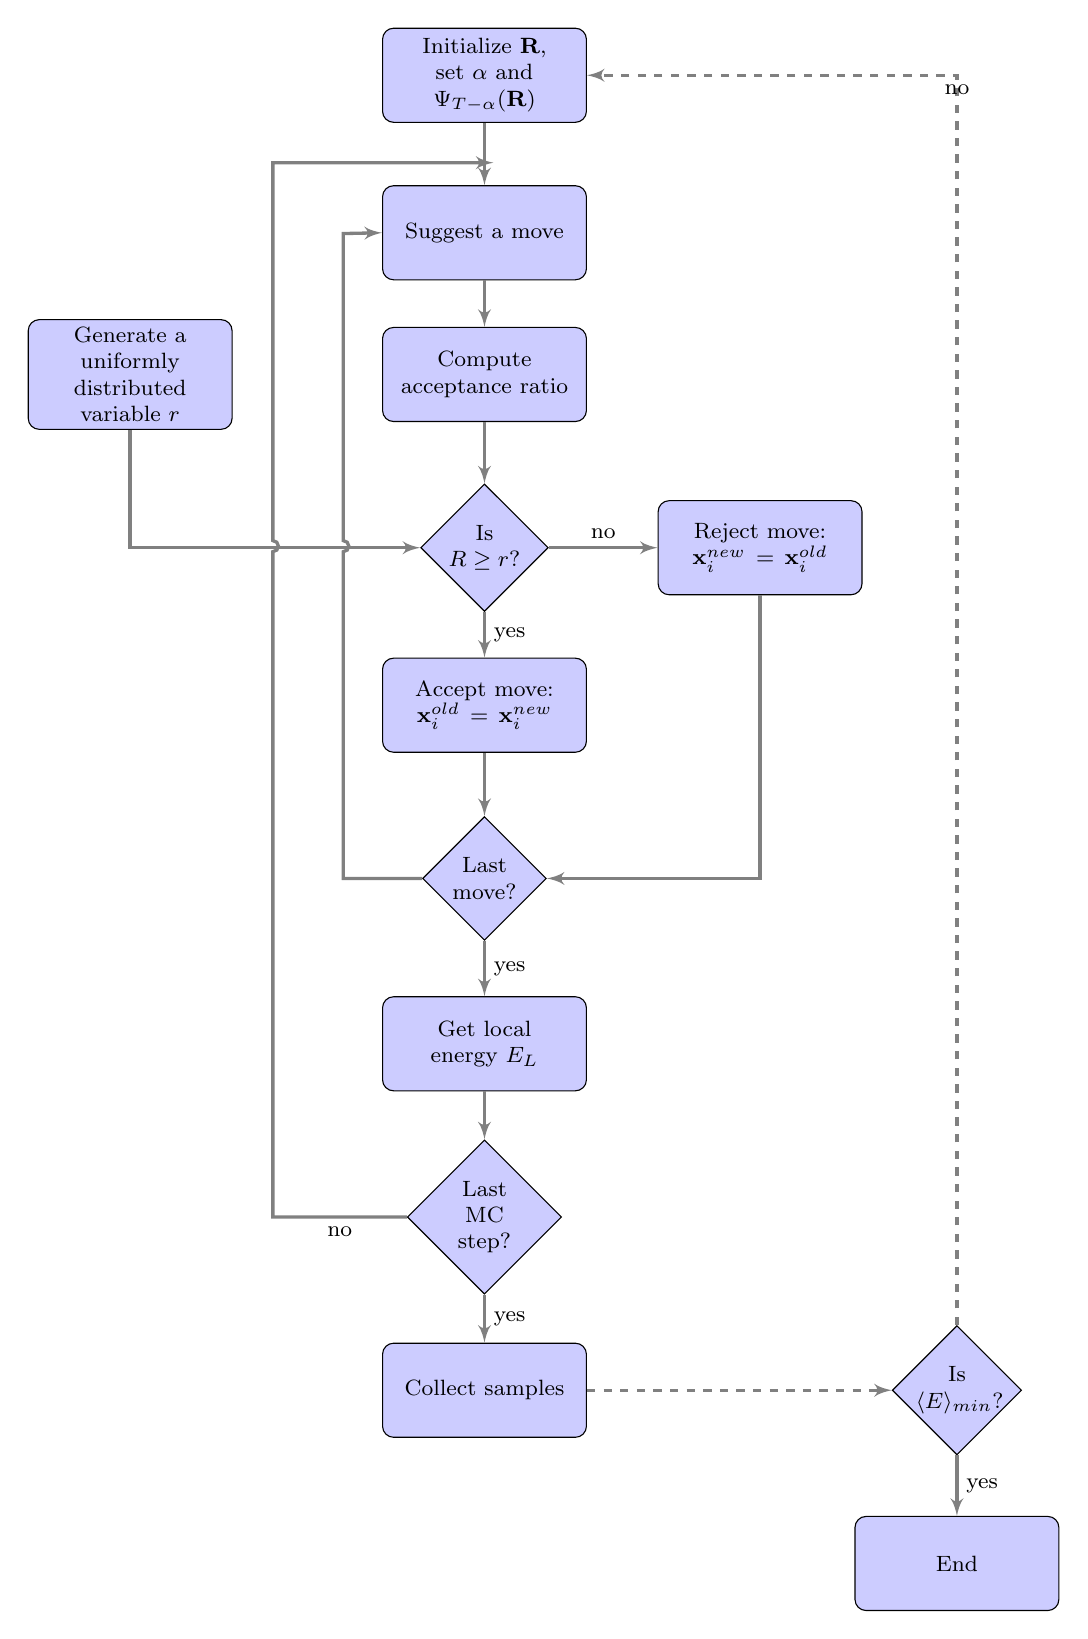
\begin{tikzpicture}[scale=1., node distance = 2.2cm, auto]
%%%%%\usebodyfont       [sansserif, 10pt]

  \footnotesize
    % Place nodes
    \node [block] (init) {Initialize ${\bf R}$,\\
    set $\alpha$ and $\Psi_{T-\alpha}({\bf R})$};
    \node [block, below of=init, node distance=2.0cm] (suggestMove) {Suggest a move};
    \node [block, below of=suggestMove, node distance=1.8cm] (evaluateAcceptance) {Compute acceptance ratio};
    \node [block, left of=evaluateAcceptance, node distance=4.5cm] (randomGenerator) {Generate a uniformly distributed variable $r$};
    \node [decision, below of=evaluateAcceptance, node distance=2.2cm] (decide) {Is\\ $R \geq r$?};
    \node [block, right of=decide, node distance=3.5 cm] (rejectMove) {Reject move: \\ ${\bf x}^{new}_{i} = {\bf x}^{old}_{i}$};
    \node [block, below of=decide, node distance=2.0cm] (acceptMove) {Accept move:\\${\bf x}^{old}_{i} = {\bf x}^{new}_{i}$};
    \node [decision, below of=acceptMove, node distance=2.2cm] (lastMove) {Last move?};
    \node [block, below of=lastMove, node distance=2.1cm] (getLocalEnergy) {Get local\\ energy $E_L$};
    \node [decision, below of=getLocalEnergy, node distance=2.2cm] (decideMC) {Last MC step?};
    \node [block, below of=decideMC, node distance=2.2cm] (collectSamples) {Collect samples};
    \node [decision, right of=collectSamples, node distance=6.0cm] (minEnergy) {Is\\ $\langle E \rangle_{min}$?};
    \node [block, below of=minEnergy] (ending) {End};
    
%     % Draw edges
    \path [line] (init) -- (suggestMove);
    \path [line] (suggestMove) -- (evaluateAcceptance);
    \path [line] (evaluateAcceptance) -- (decide);
    \path [line] (randomGenerator) |- (decide);
    \path [line] (decide) -- node [, color=black] {yes}(acceptMove);
    \path [line] (decide) -- node [, color=black] {no}(rejectMove);
    \path [line] (acceptMove) -- (lastMove); 
    \path [line] (lastMove) -- node [, color=black] {yes}(getLocalEnergy);
    \path [line] (rejectMove) |- (lastMove);
    \path [line] (getLocalEnergy) -- (decideMC);
    \path [line] (decideMC) -- node [, color=black, node distance=5.5] {yes}(collectSamples);
   

    % Define a style for shifting a coordinate upwards
    % Note the curly brackets around the coordinate.
    \tikzstyle{s}=[shift={(0mm,\radius)}]
    \path[line] (lastMove.west) -- +(-1.0,0)  -- +(-1.0, 4.15) 
% % % %     % Draw semicircle junction to indicate that the lines are
% % % %     % not connected. Since we want the semicircle to have its center 
% % % %     % where the lines intersect, we have to shift the intersection 
% % % %     % coordinate using the 's' style to account for this.
    arc(-90:90:\radius) -- +(0.0, 3.9) -- (suggestMove.west);
    
    \path [line] (decideMC.west) -- node [, color=black]{no} +(-1.7,0) --+(-1.7,8.45) 
    arc(-90:90:\radius) --+(0.0,4.8) -- +(2.8,4.8);
         
    \path [line,dashed] (collectSamples) -- (minEnergy);
    \path [line] (minEnergy) -- node [, color=black] {yes}(ending);
   \path [line,dashed] (minEnergy) |- node [, color=black] {no}(init);

\end{tikzpicture}\caption{Optimization of the trial wave function $\Psi_{trial}({\bf \alpha})$ and minimization of the energy with respect to the variational parameters.}\label{chartFlowOptim}
\end{figure}


\section{Exercises}

%\subsection*{Project 16.1: Hartree-Fock and variational Monte Carlo}

\begin{prob}
The aim of this project is to use the Variational Monte
Carlo (VMC) method and evaluate 
the ground state energy of  the atoms 
helium, beryllium and neon.

We label $r_1$ the distance from electron 1 to the nucleus and similarly 
$r_2$ the distance between electron 2 and the nucleus.
The contribution to the potential energy from the interactions between the 
electrons and the nucleus is
\be
   -\frac{2}{r_1}-\frac{2}{r_2},
\ee 
and if we add the electron-electron repulsion with
$r_{12}=|{\bf r}_1-{\bf r}_2|$, the total potential energy 
$V(r_1, r_2)$ is
\be
 V(r_1, r_2)=-\frac{2}{r_1}-\frac{2}{r_2}+
               \frac{1}{r_{12}},
\ee
yielding the total Hamiltonian
\be
   \OP{H}=-\frac{\nabla_1^2}{2}-\frac{\nabla_2^2}{2}
          -\frac{2}{r_1}-\frac{2}{r_2}+
               \frac{1}{r_{12}},
\ee
and Schr\"odinger's equation reads
\be
   \OP{H}\psi=E\psi.
\ee
All equations are in so-called atomic units. The distances
$r_i$ and $r_{12}$ are dimensionless. To have energies in electronvolt
you need to multiply all results with 
$2\times E_0$,
where $E_0=13.6$ eV.
The experimental binding energy for helium in atomic units a.u. is $E_{\mathrm{He}}=-2.9037$ a.u..


\begin{enumerate}
\item Set up the Hartree-Fock equations for the ground state of the helium atom with two electrons occupying
the hydrogen-like orbitals with quantum numbers $n=1$, $s=1/2$ and $l=0$.  There is no spin-orbit part in the two-body Hamiltonian.
{\bf Make sure to write these equations using atomic units}.  

\item  Write a program which solves the Hartree-Fock equations  for the helium atom.  Use as input for the first 
iteration the hydrogen-like single-particle wave function, with analytical shape  $\sim \exp{\left(-\alpha r_i\right)}$
where $r_i$ represents the coordinates of electron $i$. The details of all equations which you need to program will be discussed
during the lectures. Compare the results with those obtained using the hydrogen-like wave functions only.

\item   Our next step is to perform  a Variational Monte Carlo calculation of the ground state of the helium atom.
In our first attempt we will use a brute force Metropolis sampling with a trial wave function which has the following form
\begin{equation}
   \psi_{T}({\bf r_1},{\bf r_2}, {\bf r_{12}}) = 
   \exp{\left(-\alpha(r_1+r_2)\right)}
   \exp{\left(\frac{r_{12}}{2(1+\beta r_{12})}\right)}, 
\label{eq:trialxx}
\end{equation}
with $\alpha$ and $\beta$ as variational parameters.

Your task is to perform a Variational Monte Carlo calculation
using the Metropolis algorithm to compute the integral
\begin{equation}
   \langle E \rangle =
   \frac{\int d{\bf r_1}d{\bf r_2}\psi^{\ast}_T({\bf r_1},{\bf r_2}, {\bf r_{12}})\OP{H}({\bf r_1},{\bf r_2}, {\bf r_{12}})\psi_T({\bf r_1},{\bf r_2}, {\bf r_{12}})}
        {\int d{\bf r_1}d{\bf r_2}\psi^{\ast}_T({\bf r_1},{\bf r_2}, {\bf r_{12}})\psi_T({\bf r_1},{\bf r_2}, {\bf r_{12}})}.
\end{equation}
In performing the Monte Carlo analysis you should use blocking as a technique  to make the statistical analysis of the numerical data.
The code has to run in parallel. A code for doing a VMC calculation for the helium atom can be 
found on the webpage of the course, see under programs.


\item   Repeat the last step but use now  importance sampling.   Study the dependence of the results as function of the time step
$\delta t$.



\item Our final step is to replace the hydrogen-like orbits  in Eq.~(\ref{eq:trialxx}) with those obtained
from b)  by solving the Hartree-Fock equations.   This leads us to only one variational parameter, $\beta$. 
The calculations should include  parallelization, blocking and importance sampling.  There is no need to do brute
force Metropolis sampling. 

Compare the results with those from c) and the Hartree-Fock
results from b).  How important is the correlation part? 


Here we will focus on the neon and beryllium atoms.
It is convenient to make modules or classes of trial wave functions, both many-body wave functions
and single-particle wave functions  and the quantum numbers  involved,such as spin, orbital momentum and principal
quantum numbers.

The new item you need to pay attention to is the calculation of the Slater Determinant. This is an additional complication
to your VMC calculations.
If we stick to hydrogen-like wave functions,
the trial wave function for beryllium can be written as 
\begin{equation}
   \psi_{T}({\bf r_1},{\bf r_2}, {\bf r_3}, {\bf r_4}) = 
   Det\left(\phi_{1}({\bf r_1}),\phi_{2}({\bf r_2}),
   \phi_{3}({\bf r_3}),\phi_{4}({\bf r_4})\right)
   \prod_{i<j}^{4}\exp{\left(\frac{r_{ij}}{2(1+\beta r_{ij})}\right)}, 
\end{equation}
where the $Det$ is a Slater determinant and the single-particle wave functions
are the hydrogen wave functions for the $1s$ and $2s$ orbitals. Their form
within the variational ansatz are given by
\begin{equation}
\phi_{1s}({\bf r_i}) = e^{-\alpha r_i},
\end{equation}
and 
\begin{equation}
\phi_{2s}({\bf r_i}) = \left(1-\alpha r_i/2\right)e^{-\alpha r_i/2}.
\end{equation}
For neon , the trial wave function can take the form
\begin{equation}
   \psi_{T}({\bf r_1},{\bf r_2}, \dots,{\bf r_{10}}) = 
   Det\left(\phi_{1}({\bf r_1}),\phi_{2}({\bf r_2}),
   \dots,\phi_{10}({\bf r_{10}})\right)
   \prod_{i<j}^{10}\exp{\left(\frac{r_{ij}}{2(1+\beta r_{ij})}\right)}, 
\end{equation}
In this case you need to include the $2p$ wave function as well.
It is given as
\begin{equation} 
\phi_{2p}({\bf r_i}) = \alpha {\bf r_i}e^{-\alpha r_i/2}.
\end{equation}
Observe that $r_i = \sqrt{r_{i_x}^2+r_{i_y}^2+r_{i_z}^2}$.


\item Set up the Hartree-Fock equations for the ground state of the beryllium and neon atoms with four and ten  electrons, respectively,
 occupying
the respective hydrogen-like orbitals.  There is no spin-orbit part in the two-body Hamiltonian.
Find also the experimental ground state energies using atomic units.

\item Solve the Hartree-Fock equations  for the beryllium and neon atoms.  
Use again as input for the first 
iteration the hydrogen-like single-particle wave function.
Compare the results with those obtained using the hydrogen-like wave functions only (first iteration).


\item   Write a function which sets up the Slater determinant for beryllium and neon. 
Use the Hartree-Fock single-particle wave functions to set up the Slater determinant.
You have only one variational parameter, $\beta$.
Compute the ground state energies of neon  and beryllium. 
The calculations should include  parallelization, blocking and importance sampling.  Compare the results with the Hartree-Fock
results.  How important is the correlation part?  Is there a difference compared with helium?   
Comment your results.

\end{enumerate}

\end{prob}

\begin{prob}

The aim of this project is to use the Variational Monte
Carlo (VMC) method to evaluate 
the ground state energy, onebody densities, expectation values of the kinetic and potential energies  and single-particle energies of 
quantum dots with $N=2$, $N=6$ and $N=12$ electrons, so-called closed shell systems.


We consider a system of electrons confined in a pure two-dimensional 
isotropic harmonic oscillator potential, with an idealized  total Hamiltonian given by 
\begin{equation}
\label{eq:finalH}
\OP{H}=\sum_{i=1}^{N} \left(  -\frac{1}{2} \nabla_i^2 + \frac{1}{2} \omega^2r_i^2  \right)+\sum_{i<j}\frac{1}{r_{ij}},
\end{equation}
where natural units ($\hbar=c=e=m_e=1$) are used and all energies are in so-called atomic units a.u. We will study systems of many electrons $N$ as functions of the oscillator frequency  $\omega$ using the above Hamiltonian.  The Hamiltonian includes a standard harmonic oscillator part
\[
\OP{H}_0=\sum_{i=1}^{N} \left(  -\frac{1}{2} \nabla_i^2 + \frac{1}{2} \omega^2r_i^2  \right),
\]
and the repulsive interaction between two electrons given by 
\[
\OP{H}_1=\sum_{i<j}\frac{1}{r_{ij}},
\]
with the distance between electrons given by $r_{ij}=\sqrt{{\bf r}_1-{\bf r}_2}$. We define the 
modulus of the positions of the electrons (for a given electron $i$) as $r_i = \sqrt{r_{i_x}^2+r_{i_y}^2}$.


\begin{enumerate}

\item[1a)]  In exercises 1a-1e we will deal only with a system of 
two electrons in a quantum dot with a frequency of $\hbar\omega = 1$. 
The reason for this is that we have exact closed form expressions 
for the ground state energy from Taut's work for selected values of $\omega$, 
see M.~Taut, Phys. Rev. A {\bf 48}, 3561 (1993).
The energy is given by $3$ a.u.  (atomic units) when the interaction between the electrons is included.
If only the harmonic oscillator part of the Hamiltonian,
the so-called unperturbed part,
\[ \OP{H}_0=\sum_{i=1}^{N} \left(  -\frac{1}{2} \nabla_i^2 + \frac{1}{2} \omega^2r_i^2  \right),\]
the energy is $2$ a.u.
The wave function for one electron in an oscillator potential in two dimensions is
\[
\phi_{n_x,n_y}(x,y) = A H_{n_x}(\sqrt{\omega}x)H_{n_y}(\sqrt{\omega}y)\exp{(-\omega(x^2+y^2)/2}.
\]
The functions $H_{n_x}(\sqrt{\omega}x)$ are so-called Hermite polynomials, discussed in appendix while $A$ is a normalization constant. 
For the lowest-lying state we have $n_x=n_y=0$ and an energy $\epsilon_{n_x,n_y}=\omega(n_x+n_y+1) = \omega$.
Convince yourself that the lowest-lying energy for the two-electron system  is simply $2\omega$.

The unperturbed wave function for the ground state of the two-electron system is given by 
\[
\Phi({\bf r_1},{\bf r_2}) = C\exp{\left(-\omega(r_1^2+r_2^2)/2\right)},
\]
with $C$ being a normalization constant and $r_i = \sqrt{r_{i_x}^2+r_{i_y}^2}$. Note that the vector ${\bf r_i}$ 
refers to the $x$ and $y$ position for a given particle.
What is the total spin of this wave function? Find arguments for why the ground state should have
this specific total spin. 

\item[1b)] We want to perform  a Variational Monte Carlo calculation of the ground state of two electrons in a quantum dot well with different oscillator energies, assuming total spin $S=0$ using the Hamiltonian of 
Eq.~(\ref{eq:finalH}). 
In our first attempt we will use a brute force Metropolis sampling with a trial wave function which has the following form
\begin{equation}
   \psi_{T}({\bf r_1},{\bf r_2}) = 
   C\exp{\left(-\alpha\omega(r_1^2+r_2^2)/2\right)}
   \exp{\left(\frac{ar_{12}}{(1+\beta r_{12})}\right)}, 
\label{eq:trial}
\end{equation}
where $a$ is equal to one when the two electrons have anti-parallel spins and $1/3$ when the spins are parallel. Finally, $\alpha$ and $\beta$ are our variational parameters.

Your task is to perform a Variational Monte Carlo calculation
using the Metropolis algorithm to compute the integral
\begin{equation}
   \langle E \rangle =
   \frac{\int d{\bf r_1}d{\bf r_2}\psi^{\ast}_T({\bf r_1},{\bf r_2})\OP{H}({\bf r_1},{\bf r_2})\psi_T({\bf r_1},{\bf r_2})}
        {\int d{\bf r_1}d{\bf r_2}\psi^{\ast}_T({\bf r_1},{\bf r_2})\psi_T({\bf r_1},{\bf r_2})}.
\end{equation}
You should parallelize your program. As an optional possibility, to program GPUs can be used 
instead of standard parallelization with MPI throughout the project.

Find the  energy minimum and compute also the mean distance
$r_{12}=\sqrt{{\bf r}_1-{\bf r}_2}$ (with $r_i = \sqrt{r_{i_x}^2+r_{i_y}^2}$) between the two electrons for the optimal set of the variational parameters.
A code for doing a VMC calculation for a two-electron system (the three-dimensional helium atom) can be 
found on the webpage of the course, see under programs.

You should also find a closed-form expression for the local energy. Compare the results of this calculation (in terms of CPU time) compared with a calculation which performs a brute force numerical derivation.
\item[1c)] Introduce now importance sampling and study the dependence of the results as a function of the time step $\delta t$.  
Compare the results with those obtained under 1a) and comment eventual differences.
In performing the Monte Carlo analysis you should use blocking as a technique  to make the statistical analysis of the numerical data.
The code has to run in parallel. 
\item[1d)]  With the optimal parameters for the ground state wave function, compute the onebody density. Discuss your results and compare the results with those obtained with a pure harmonic oscillator wave functions. Run a Monte Carlo calculations without the Jastrow factor as well
and compute the same quantities. How important are the correlations induced by the Jastrow factor?
Compute also the expectation value of the kinetic energy and potential energy using $\omega=0.01$,
$\omega=0.28$ and $\omega=1.0$. Comment your results.
\item[1e)]  Repeat step 1c) by varying the energy using the 
conjugate gradient method to obtain the best possible set of parameters
$\alpha$ and $\beta$. Discuss the results.
\end{enumerate}
The previous exercises have prepared you for extending your calculational machinery  to other systems.
Here we will focus on quantum dots with $N=6$ and $N=12$ electrons.
It is convenient to make modules or classes of trial wave functions, both many-body wave functions
and single-particle wave functions  and the quantum numbers  involved, such as spin, value of $n_x$ and $n_y$
quantum numbers.

The new item you need to pay attention to is the calculation of the Slater Determinant. This is an additional complication
to your VMC calculations.
If we stick to harmonic oscillator like wave functions,
the trial wave function for say an $N=6$ electron quantum dot can be written as 
\begin{equation}
   \psi_{T}({\bf r_1},{\bf r_2},\dots, {\bf r_6}) = 
   Det\left(\phi_{1}({\bf r_1}),\phi_{2}({\bf r_2}),
   \dots,\phi_{6}({\bf r_6})\right)
   \prod_{i<j}^{6}\exp{\left(\frac{a r_{ij}}{(1+\beta r_{ij})}\right)}, 
\end{equation}
where $Det$ is a Slater determinant and the single-particle wave functions
are the harmonic oscillator wave functions for the $n_x=0,1$ and $n_y=0,1$ orbitals. 
For the $N=12$ quantum dot, the trial wave function can take the form
\begin{equation}
   \psi_{T}({\bf r_1},{\bf r_2}, \dots,{\bf r_{12}}) = 
   Det\left(\phi_{1}({\bf r_1}),\phi_{2}({\bf r_2}),
   \dots,\phi_{12}({\bf r_{12}})\right)
   \prod_{i<j}^{12}\exp{\left(\frac{ar_{ij}}{2(1+\beta r_{ij})}\right)}, 
\end{equation}
In this case you need to include the $n_x=2$ and $n_y=2$ wave functions as well.
Observe that $r_i = \sqrt{r_{i_x}^2+r_{i_y}^2}$.  Use the Hermite polynomials defined in the appendix.


\begin{enumerate}
\item[(1f)]   Write a function which sets up the Slater determinant 
handle larger systems as well. Find the Hermite polynomials which are needed for $n_x=0,1,2$ and obviously $n_y$ as well.
Compute the ground state energies of quantum dots for $N=6$ and $N=12$ electrons, following the same set up as in exercise 1e) for $\omega=0.01$,
$\omega=0.28$ and $\omega=1.0$.
The calculations should include  parallelization, blocking, importance sampling and energy minimization using the conjugate gradient approach.
To test your Slater determinant code, you should reproduce the unperturbed single-particle energies
when the electron-electron repulsion is switched off. Convince yourself that the unperturbed ground state energies for $N=6$ is $10\omega$ and for $N=12$ we obtain $28\omega$.  What is the expected total 
spin of the ground states?
  
\item[1g)]  With the optimal parameters for the ground state wave function, compute again the onebody density. Discuss your results and compare the results with those obtained with a pure harmonic oscillator  
wave functions. Run a Monte Carlo calculations without the Jastrow factor as well
and compute the same quantities. How important are the correlations induced by the Jastrow factor?
Compute also the expectation value of the kinetic energy and potential energy using $\omega=0.01$,
$\omega=0.28$ and $\omega=1.0$. Comment your results.
\end{enumerate}

\section*{Additional material on Hermite polynomials}

The Hermite polynomials are the solutions of the following differential
equation
\be
   \frac{d^2H(x)}{dx^2}-2x\frac{dH(x)}{dx}+
       (\lambda-1)H(x)=0.
   \label{eq:hermite}
\ee
The first few polynomials are
\[
   H_0(x)=1,
\]
\[
    H_1(x)=2x,
\]
\[
    H_2(x)=4x^2-2,
\]
\[
    H_3(x)=8x^3-12x,
\]
and
\[
    H_4(x)=16x^4-48x^2+12.
\]
They fulfil the orthogonality relation
\[
  \int_{-\infty}^{\infty}e^{-x^2}H_n(x)^2dx=2^nn!\sqrt{\pi},
\]
and the recursion relation
\[
  H_{n+1}(x)=2xH_{n}(x)-2nH_{n-1}(x).
\]
\end{prob}

 \clearemptydoublepage
\chapter{Bose-Einstein condensation and Diffusion Monte Carlo}\label{chap:advancedqmc}
\abstract{We discuss how to perform diffusion Monte Carlo calculations for systems of bosons}

\section{Diffusion Monte Carlo}

The DMC method belongs to a larger class of methods often called
\emph{projector} Monte Carlo. As the name indicates, this is a general
class of methods based on taking projections in Hilbert space.

%From a given superposition $\Psi$ of eigenfunctions of $\op H$, we
%will project out the desired one:
%\bdm
%\Psi = \sum_i c_i \phi_i \to \phi_k
%\edm

Consider a system governed by a Hamiltonian $\op H$. Its stationary
eigenfunctions are then given by
\bdm
\op H\phi_i = \epsilon_i\phi_i
\edm
DMC is a method of projecting out the $\phi_i$ from $\Psi$ with the
lowest energy. Most often, and in our case particularly, we are
interested in the ground state. But just as with the variational
principle used by VMC, if we let $\Psi$ fulfill a certain mathematical
symmetry, the projected $\phi_k$ will be the state of lowest energy
with that given symmetry.

In contrast to VMC, which relies on the variational principle, DMC does not directly depend on any a
priori choice of wave function that ultimately restricts the quality
of the result. Thus, DMC can in principle produce the exact ground
state of our system, at least within the statistical limits of the
algorithm.

The procedure of projecting out the component state of $\Psi$ with the
lowest energy is based on operating on $\Psi$ with the special
evolution operator $\exp(-\op Ht)$
\bdm
e^{(-\op Ht)}\Psi(\vec x) = \sum_i c_i
\exp(-\epsilon_it)\phi_i(\vec x)
\edm
This is just the formal solution of the special equation:
\be
-\frac{\partial}{\partial t}\Psi(\vec x, t) =
\op H \Psi(\vec x, t)
\label{eq:SE_imaginary_time}
\ee
which resembles the time dependent Schr\"odinger equation as if it
were transformed to imaginary time $it\to t$. Recall that the formal
solution of the time dependent Schr\"odinger equation is just
\bdm
\Psi(\vec x, t) = e^{-\frac{i}{\hbar}\op Ht}\,\Psi(\vec x) =
\sum_i c_i e^{-\frac{i}{\hbar}\epsilon_it}\,\phi_i(\vec x)
\edm
As we let $t\to\infty$, the exponential makes all the eigenstates with
negative energy blow up while the ones with positive energy vanish. To
control this effect we introduce a constant energy shift 
$E_{\mathrm{T}}$, called a \emph{trial energy}, to the potential term
of $\op H$. This shift does, of course, not change any relevant physical
properties of our system since it is generally independent of the
choice of the zero point of the energy. The effect on the projection
operation becomes
\be
\Psi(\vec x, t) =
e^{-(\op H - E_{\mathrm{T}})t}\Psi(\vec x) = \sum_i c_i
e^{-(\epsilon_i-E_{\mathrm{T}})t}\phi_i(\vec x)
\label{eq:projector_on_Psi}
\ee
Consider the ideal situation of letting $E_{\mathrm{T}}$ equal exactly
$\epsilon_0$, resulting in
\bdm
\Psi(\vec x, t) =
e^{-(\op H - E_{\mathrm{T}})t}\Psi(\vec x) =
c_0\phi_0 + \sum_{i>0}c_i\phi_i(\vec x)e^{-(\epsilon_i-\epsilon_0)t}
\edm
Since $\epsilon_i > \epsilon_0$ for $i \neq 0$, all the remaining
exponents become negative. In the limit $t\to\infty$, the
contributions from excited states must obviously vanish, so that
propagating $\Psi$ according to Eq.~(\ref{eq:SE_imaginary_time})
gives
\bdm
\lim_{t\to\infty} e^{-(\op H - \epsilon_0)t}\Psi(\vec x) =
c_0\phi_0
\edm
thus projecting out the ground state.

Without even considering how to do the time propagation in practice,
the formulas already indicate to us that approaching the problem first
with VMC can help produce an initial $\Psi$ close to $\phi_0$ and,
more importantly, a trial energy $E_{\mathrm{T}}$ being an upper bound
to the true ground state energy $\epsilon_0$. Hopefully
$E_{\mathrm{T}}$ is close enough to $\epsilon_0$ to be smaller than the
first excited energy. Inserting such a $E_{\mathrm{T}}$ into
Eq.~(\ref{eq:projector_on_Psi}) while letting $t\to\infty$ will make all
the excited states collapse while the ground state blows up and
dominates because of the positive exponent in the coefficient.

From this consideration we also see that the evolution operator is not
unitary. The norm of $\Psi$ is not necessarily conserved with time.
Depending on the value of $E_{\mathrm{T}}$ it may grow without limit
or go to zero. Only in the case of $E_{\mathrm{T}}=\epsilon_0$ the
state tends to a constant. This proposes a method of determining the
ground state energy by adjusting $E_{\mathrm{T}}$ dynamically during
time propagation so that the state stays constant.

Writing out the imaginary time Schr\"odinger equation,
Eq.~(\ref{eq:SE_imaginary_time}), including the energy offset 
$E_\mathrm{T}$, we get
\bea
\frac{\partial}{\partial t}\Psi(\vec x, t) &=&
-\op K \Psi(\vec x, t) -
(\op V(\vec x) - E_\mathrm{T})\Psi(\vec x, t)\nonumber\\
&=&
\frac{\hbar^2}{2m}\nabla^2 \Psi(\vec x, t) -
(\op V(\vec x) - E_\mathrm{T})\Psi(\vec x, t)
\label{eq:SE_imaginary_time_expanded}
\eea
where $\op K$ and $\op V$ is the kinetic and potential energy
operator, respectively. We see that this is of the form of an extended
diffusion equation. We can therefore consider the wave function $\Psi$
as a probability distribution evolving according to this equation.
This greatly contrasts the usual quantum mechanical interpretation of
$|\Psi|^2$ being the actual probability density function (PDF). We
will see that the approach poses some potentially serious problems
when the wave function $\Psi$ we seek has nodes and is partially
negative and possibly complex. But to illustrate the main mechanisms
of the method we will at the moment focus on the simple cases of
bosonic ground states which usually are strictly positive and real.

In simple terms, the job consists of representing the initial state
$\Psi$ by a collection of walkers, much the same way as in VMC, and
letting them evolve in time as a controlled diffusion process governed
by Eq.~(\ref{eq:SE_imaginary_time_expanded}). Interpreting the
rhs.~terms of Eq.~(\ref{eq:SE_imaginary_time_expanded}), we see that
the first term is a standard diffusion term with a diffusion constant
of
\be
D\equiv\frac{\hbar^2}{2m}
\label{eq:diffusion_constant}
\ee
The second term is called a \emph{branching term}. When positive, it
induces a growth of the number of walkers and a decay if it is negative.

Before we expand on how to carry out DMC in practice, it may be
helpful to consider an analytically exact approach by focusing on the
Green's function corresponding to the time evolution of the wave function. 
The approach is called
\emph{Green's function Monte Carlo} (GFMC) and shares its main ideas
with the DMC method. Using Dirac's bracket notation, we start over by
substituting the initial wave function $\Psi(\vec x)$ with its
corresponding state ket $|\Psi\rangle$ and let the special evolution
operator work on $|\Psi\rangle$
\bdm
|\Psi\rangle_t = e^{-(\op H - E_{\mathrm{T}})t}|\Psi\rangle,
\edm
Now we switch to position representation:
\bdm
\Psi(\vec x, t) =
\overlap{\vec x}{\Psi}_t =
\bracket{\vec x}{e^{-(\op H - E_{\mathrm{T}})t}}{\Psi} =
\int\bracket{\vec x}{e^{-(\op H - E_{\mathrm{T}})t}}{\vec x^\prime}
\overlap{\vec x^\prime}{\Psi}d\vec x^\prime
\edm
where we have just inserted a completeness relation,
$1=\int\projection{\vec x^\prime}{\vec x^\prime}\,d\vec x^\prime$.
Defining the Green's function for this case
\bdm
G(\vec x,\vec x^\prime,t) \equiv
\bracket{\vec x}{e^{-(\op H - E_{\mathrm{T}})t}}{\vec x^\prime} =
\bracket{\vec x}{e^{-(\op K + \op V - E_{\mathrm{T}})t}}
{\vec x^\prime}
\edm
we get:
\be
\Psi(\vec x, t) =
\int G(\vec x,\vec x^\prime,t)\Psi(\vec x^\prime)d\vec x^\prime
\label{eq:greens_function_propag}
\ee
Calculating the Green's function $G$ would be greatly simplified if we
could split it into separate factors for each of the terms $\op K$ and
$(\op V- E_\mathrm{T})$ of the Hamiltonian $\op H$, as with the
following factorization
\bdm
e^{\op A + \op B} = e^{\op A}\,e^{\op B}
\edm
However, such a factorization requires that the operators $\op A$ and
$\op B$ commute, $[A,B]=0$. Unfortunately, this is not the case for
the terms $\op K$ and $\op V$ of the Hamiltonian. But, by expanding
the exponential of each part, using a descendent of the so called
Baker-Campbell-Hausdorff formula
\bdm
e^{\op A}e^{\op B}=e^{\op A+\op B}e^{\frac{1}{2}[\op A,\op B]}
\edm
we get that:
\bdm
e^{-(\op H-E_{\mathrm{T}})t} = e^{-(\op K+\op V-E_{\mathrm{T}})t} =
e^{-\op K t}e^{-(\op V-E_{\mathrm{T}}) t} + \bigO(t^2)
\edm
It is also possible to make approximations to higher orders of $t$, but
we will here keep to the simple first order case. As $t\to 0$, the error
term disappears and the simple factorized form becomes exact. Thus, an
approximation of the form
\bdm
e^{-(\op H-E_{\mathrm{T}})t}\approx
e^{-\op K t}e^{-(\op V-E_{\mathrm{T}}) t}
\edm
is only good for small $t$ and is readily called a \emph{short time
  approximation}. The Green's function can by this be approximated as
follows
\beaN
G(\vec x,\vec x^\prime,t) &=&
\bracket{\vec x}{e^{-(\op H-E_{\mathrm{T}})t}}{\vec x^\prime}\\
&=&
\bracket{\vec x}{e^{-\op K t}\,e^{-(\op V-E_{\mathrm{T}}) t}}
{\vec x^\prime} + \bigO(t^2)\\
&=&
\int\bracket{\vec x}{e^{-\op K t}}{\vec x^{\prime\prime}}\,
\bracket{\vec x^{\prime\prime}}{e^{-(\op V-E_{\mathrm{T}}) t}}
{\vec x^\prime}\,d\vec x^{\prime\prime} + \bigO(t^2)\\
&=&
\int G_K(\vec x,\vec x^{\prime\prime},t)\,
G_V(\vec x^{\prime\prime},\vec x^\prime,t)
\,d\vec x^{\prime\prime} + \bigO(t^2)
\eeaN
For the kinetic energy part, $G_K$, we get
\beaN
G_K(\vec x,\vec x^{\prime\prime},t) &=&
\bracket{\vec x}{e^{-\op K t}}{\vec x^{\prime\prime}}\\
&=&
\frac{1}{(2\pi)^{3N}}\int
\overlap{\vec x}{\vec k}e^{-Dk^2t}
\overlap{\vec k}{\vec x^{\prime\prime}}\,d\vec k\\
&=&
\frac{1}{(2\pi)^{3N}}\int
e^{-i\vec k\vec x}e^{-Dk^2t}
e^{i\vec k\vec x^{\prime\prime}}\,d\vec k\\
&=&
\frac{1}{(4\pi Dt)^{3N/2}}\,
e^{-(\vec x^{\prime\prime}-\vec x)^2/4Dt}
\eeaN
The constant $D$ is still the same diffusion constant in
Eq.~(\ref{eq:diffusion_constant}). The part related to the potential,
$G_V$, is simpler, since it contains a local operator only dependent
on $\vec x$
\bdm
G_V(\vec x^{\prime\prime},\vec x^\prime,t) =
e^{-(V(\vec x^\prime)-E_{\mathrm{T}})t}
\delta(\vec x^\prime-\vec x^{\prime\prime})
\edm
Putting these two parts together and carrying out the integral over
$\vec x^{\prime\prime}$ is simplified by the delta function of
$G_V$. Ignoring the normalization constant of $G_K$ we get
\be
G(\vec x,\vec x^\prime,t) =
e^{-(\vec x^\prime-\vec x)^2/4Dt}\,
e^{(E_\mathrm{T}-V(\vec x^\prime))t}+\bigO(t^2)
\label{eq:greens_func_short_time}
\ee

At this point, the GFMC method would pursue the problem by explicitly
evaluating the Green's function integral of
Eq.~(\ref{eq:greens_function_propag}) with a suitable
approximation. We, on the other hand, are now ready to interpret the
diffusion process controlled by
Eq.~(\ref{eq:SE_imaginary_time_expanded}) in terms of the short time
approximated Green's function. Our wave function $\Psi(\vec x)$ is
represented by a set of random walkers, so the integral over $G(\vec
x,\vec x^\prime,t)\Psi(\vec x^\prime)$ expresses the probability of a
walker ending up at $\vec x$ given the initial configuration of
walkers $\Psi(\vec x^\prime)$.  Calculating the integral corresponds
to one iteration of the DMC algorithm (to be described in detail later
on). Operationally this has a different effect for each of the two
exponential factors of $G$.

The first factor expresses the probability for a walker to move from
position $\vec x$ to $\vec x^\prime$. Since this clearly is just a
Gaussian of $\vec x$ around $\vec x^\prime$, we can simply generate
new positions as a simple diffusion process
\bdm
\vec x = \vec x^\prime + \chi
\edm
where $\chi$ is a Gaussian pseudo-random number with mean equal zero
and variance equal $2Dt$. The second factor, the branching term, is
only dependent on $\vec x^\prime$ and can be interpreted as the rate
of growth of random walkers at each position $\vec x^\prime$. The
short time approximation permits us to conduct the two processes,
diffusion and branching separately, as long as the time step $t$ is
kept small.

Even though this approach, after a large enough number of iterations,
should yield a distribution of walkers corresponding to the exact
ground state of $\op H$, the method is not efficient. In particular, a
serious problem arises when our system is governed by an unbounded
potential, like a Coulomb potential typical for interactions between
electrons or a parametrized nucleon-nucleon central potential 
with a hard central core. The branching
exponential may diverge giving a huge production of new random walkers
that may be difficult to handle numerically. Also the fluctuations
become very large making statistical estimates of physical quantities
inaccurate.

Another problem is that there is actually no simple way of calculating
a mean energy estimate from the set of walkers alone. The mean energy
is not only the most essential result of the algorithm, we also need
it to be able to adjust the trial energy $E_\mathrm{T}$ dynamically
throughout the DMC calculation.

For these reasons, and others that will become apparent, we introduce
so called importance sampling by biasing the combined
branching-diffusion process with a trial wave function
$\Psi_\mathrm{T}$ which hopefully imitates the exact solution well.
The technical contents of this will be made clear shortly.


\subsection{Importance Sampling}

Let us
introduce a time independent trial wave function $\Psi_\mathrm{T}(\vec
x)$. We define the new quantity
\bdm
f(\vec x, t) \equiv \Psi_\mathrm{T}(\vec x)\,\Psi(\vec x, t)
\edm
Now by inserting $\Psi=f/\Psi_\mathrm{T}$ into
Eq.~(\ref{eq:SE_imaginary_time_expanded}) we get a slightly more
complicated equation in terms of $f(\vec x,t)$
\be
\frac{\partial f(\vec x, t)}{\partial t} =
D\nabla^2 f(\vec x, t)-D\vec\nabla(\vec F(\vec x)f(\vec x, t))-
(E_{\mathrm{L}}(\vec x)-E_{\mathrm{T}})f(\vec x, t)
\label{eq:SE_imaginary_time_expanded_imp}
\ee
with the constant $D$ defined as in
Eq.~(\ref{eq:diffusion_constant}). Notice that the
rhs.~consists of three terms. By the same line of thought as before
we now recognize the first term as the familiar diffusion term, acting
on $f$ instead of $\Psi$. The last term, similar in form to the
potential term, is our new branching term, also acting on $f$. The
quantity $E_\mathrm{L}(\vec x)$ is just the local energy with respect
to $\Psi_{\mathrm{T}}$, defined in the same manner as in the variational Monte Carlo procedure
\bdm
E_{\mathrm{L}} \equiv
\frac{1}{\Psi_\mathrm{T}}\op H\Psi_\mathrm{T}
\edm
The vector quantity $\vec F(\vec x)$ in the unfamiliar middle term is
the drift velocity as we know it from the Fokker-Planck formalism we
used to improve the Metropolis algorithm
\be
\vec F(\vec x)\equiv
\frac{2}{\Psi_\mathrm{T}}\vec\nabla\Psi_\mathrm{T}
\label{eq:drift_velocity_DMC}
\ee
Actually, the two first terms on the rhs.~of
Eq.~(\ref{eq:SE_imaginary_time_expanded_imp}) can equivalently be
expressed as the familiar Fokker-Planck drift-diffusion on the rhs.~of
Eq.~(\ref{eq:fokker-planck}).

Eq.~(\ref{eq:SE_imaginary_time_expanded_imp}) motivates us to let the
set of random walkers represent $f$ instead of $\Psi$. A typical first
order short time approximation of the corresponding Green's function
is
\bea
G(\vec x,\vec x^\prime,t) &=&
\frac{1}{(4\pi Dt)^{3N/2}}\,
e^{-(\vec x-\vec x^\prime-Dt\vec F(\vec x^\prime))^2/4Dt}\,\,
e^{-((E_\mathrm{L}(\vec x)+E_\mathrm{L}(\vec
  x^\prime))/2-E_\mathrm{T})t}\nonumber\\&+&
\vphantom{\frac{1}{1}}\bigO(t^2)
\label{eq:greens_func_short_time_imp}
\eea
We see that the Green's function above
consists of two factors. The first one is similar to the Gaussian in
Eq.~(\ref{eq:greens_func_short_time}). But now we have in addition a
drift term displacing the mean of the Gaussian by $Dt\vec F(\vec
x^\prime)$. Notice that this factor of the Green's function is
practically identical to the transition proposition rule introduced by
the Fokker-Planck formalism to improve the Metropolis algorithm
(see Eq.~(\ref{eq:omega_drift_diffusion})). We can therefore use the same
drift-diffusion formalism for the first factor in the above Green's
function. Recall that if a walker is initially at position $\vec
x^\prime$, the new position $\vec x$ is calculated as follows (see
Eq.~(\ref{eq:drift_diffusion_proposition}))
\be
\vec x = \vec x^\prime + \chi +
D\vec F(\vec x^\prime) t
\label{eq:drift_diffusion_prop_DMC}
\ee
where $\chi$ is again a Gaussian pseudo-random number with mean equal
zero and variance equal $2Dt$ while $D\vec F(\vec x^\prime) t$ gives a
drift in the direction that $\Psi_\mathrm{T}$ increases. The size of the time step
$t$ biased the final outcome of the Fokker-Planck algorithm of the
drifted diffusion. A desirable diffusion was reached only as $t\to 0$
for each iteration. Also in the present application to DMC, this bias
must be taken into account. In the Metropolis algorithm, the
rejection mechanism took care of it. So we may use the same approach
here. After calculating a new position with
Eq.~(\ref{eq:drift_diffusion_prop_DMC}), we accept it according to the
acceptance matrix
\be
  A(\vec x ,\, \vec x^\prime,\, t) = 
  \textrm{min}\left[1\textrm{, }
  \frac{G_K(\vec x^\prime, \vec x)}
  {G_K(\vec x, \vec x^\prime)}
  \frac{|\Psi_\mathrm{T}(\vec x)|^2}
       {|\Psi_\mathrm{T}(\vec x^\prime)|^2}\right]
  \label{eq:acceptance_DMC}
\ee
where $G_K$ is the kinetic part of the Green's function, the part
related to the diffusion process. If we do not wish to do such a
Metropolis test, we may alternatively conduct separate calculations
for a set of different time steps $t$ and extrapolate the results to
$t=0$.

The second factor of Eq.~(\ref{eq:greens_func_short_time_imp}) plays
the same role as the branching term of
Eq.~(\ref{eq:greens_func_short_time}). But the potential $V$ is
replaced by an expression dependent on the local energy,
\bdm
\frac{E_\mathrm{L}(\vec x)+E_\mathrm{L}(\vec x^\prime)}{2}-
E_\mathrm{T}
\edm

The new branching term gives a greatly reduced branching effect
compared to the one in Eq.~(\ref{eq:greens_func_short_time}).
Particularly, in the limit of $\Psi_\mathrm{T} = \phi_0$ and
$E_\mathrm{T}=\epsilon_0$ (exactly equal the ground state of $\op H$),
the local energy is constant, giving equal branching everywhere, or in
effect, no branching at all. Thus we can in general expect the number
of walkers to fluctuate less and we certainly avoid uncontrollable
growth. In addition, the branching favors the areas of the
configuration space that give the lowest local energy, i.e.~the local
energy closest to the true ground state energy. Furthermore, the drifted
diffusion pushes the walkers towards the desirable areas. Thus the
whole DMC process is conducted more efficiently.

Finally, the introduction of the trial wave function $\Psi_\mathrm{T}$
makes it possible to evaluate an estimate of the mean energy given the
distribution of the walkers. Instead of calculating the typical mean
energy
\bdm
\frac{\int\Psi^\ast\op H\Psi d\vec x}
{\int\Psi^\ast\Psi d\vec x}
\edm
we calculate the so called \emph{mixed estimator}
\be
\mean{E}_\mathrm{mixed} = 
\frac{\int\Psi_\mathrm{T}\op H\Psi d\vec x}
{\int\Psi_\mathrm{T}\Psi d\vec x}
\label{eq:mixed_estim}
\ee
As the DMC method approaches the exact result $\Psi=\phi_0$, the mixed
estimator becomes
\bdm
\mean{E}_\mathrm{mixed} =
\frac{\int\Psi_\mathrm{T}\,\epsilon_0\,\Psi d\vec x}
{\int\Psi_\mathrm{T}\Psi d\vec x} =
\frac{\epsilon_0\int\Psi_\mathrm{T}\Psi d\vec x}
{\int\Psi_\mathrm{T}\Psi d\vec x} =
\epsilon_0
\edm
so that the estimate indeed becomes correct.  Because of the
hermiticity of $\op H$ we can rewrite the mixed estimator of
Eq.~(\ref{eq:mixed_estim}) as follows
\be
\mean{E}_\mathrm{mixed} = 
\frac{\int\Psi\op H\Psi_\mathrm{T} d\vec x}
{\int\Psi_\mathrm{T}\Psi d\vec x} =
\frac{\int\Psi_\mathrm{T}\Psi\,\frac{1}{\Psi_\mathrm{T}}
\op H\Psi_\mathrm{T}\,d\vec x}
{\int\Psi_\mathrm{T}\Psi d\vec x}=
\frac{\int E_\mathrm{L}f(\vec x) d\vec x}
{\int f(\vec x) d\vec x}
\label{eq:mixed_estim_Elocal}
\ee
Since the walkers represent $f$ we just need to average the local
energy $E_\mathrm{L}$ over the set of walkers.

This energy estimator allows us to calculate relatively easily the mean
energy on the distribution of walkers so that we can update the trial
energy $E_{\mathrm{T}}$ dynamically as the algorithm proceeds. As
the trial energy gets better and better, the algorithm will hopefully
stabilize on the exact result within the limits of statistical
fluctuations imposed by the local energy and our choice of
$\Psi_\mathrm{T}$.

As we know, a good choice of $\Psi_\mathrm{T}$ reduces the
fluctuations of the local energy $E_\mathrm{L}$. Now we see that this
also makes the estimation of the mean energy
in Eq.~(\ref{eq:mixed_estim_Elocal}) more efficient since the same
number of points (walkers) gives a smaller variance, thus pinpointing
the energy more exactly.

Importance sampling makes it also to some extent easier to deal with
wave functions that are not positive definite, like fermionic states
whose wave function have nodes. What happens is that the nodes of the
function $f$ are tied by the nodes of the trial wave function
$\Psi_\mathrm{T}$. Therefore it is necessary for $\Psi_\mathrm{T}$ to
have a node configuration that best reproduces the physical properties
of the exact wave function. Operationally, the node surfaces of
$\Psi_\mathrm{T}$ become impenetrable walls to the walkers in the
sense that the drift velocity $\vec F$ in the vicinity of such a
surface increases in a direction away from it pushing any walker away,
preventing it from crossing the nodal surfaces of $\Psi_\mathrm{T}$.
The approach is called a \emph{fixed node approximation}.

From all these deliberations on importance sampling we should by now
understand the importance of the trial wave function being as close to
the exact solution as possible. We therefore rely heavily on simpler
methods like VMC that do not necessarily solve the problem exactly,
but are easier to handle computationally and are much less sensitive
to initial conditions.


%\subsection{A Summary of the Algorithm}
%In preparation for spring 2010.

\section{Bose-Einstein Condensation in Atoms}

 


 The spectacular demonstration of Bose-Einstein condensation (BEC) in gases of
 alkali atoms $^{87}$Rb, $^{23}$Na, $^7$Li confined in magnetic
 traps \cite{anderson95,davis95,bradley95} has led to an explosion of interest in
 confined Bose systems. Of interest is the fraction of condensed atoms, the
 nature of the condensate, the excitations above the condensate, the atomic
 density in the trap as a function of Temperature and the critical temperature of BEC,
 $T_c$. The extensive progress made up to early 1999 is reviewed by Dalfovo et
 al.\cite{dalfovo1999}.

 A key feature of the trapped alkali and atomic hydrogen systems is that they are
 dilute. The characteristic dimensions of a typical trap for $^{87}$Rb is
 $a_{h0}=\left( {\hbar}/{m\omega_\perp}\right)^\frac{1}{2}=1-2 \times 10^4$
 \AA\ (Ref.~\cite{anderson95}). The interaction between $^{87}$Rb atoms can be well represented
 by its s-wave scattering length, $a_{Rb}$. This scattering length lies in the
 range $85 < a_{Rb} < 140 a_0$ where $a_0 = 0.5292$ \AA\ is the Bohr radius.
 The definite value $a_{Rb} = 100 a_0$ is usually selected and
 for calculations the definite ratio of atom size to trap size 
 $a_{Rb}/a_{h0} = 4.33 \times 10^{-3}$ 
 is usually chosen \cite{dalfovo1999}. A typical $^{87}$Rb atom
 density in the trap is $n \simeq 10^{12}- 10^{14}$ atoms/cm$^3$ giving an
 inter-atom spacing $\ell \simeq 10^4$ \AA. Thus the effective atom size is small
 compared to both the trap size and the inter-atom spacing, the condition
 for diluteness ($na^3_{Rb} \simeq 10^{-6}$ where $n = N/V$ is the number
 density). In this limit,
 although the interaction is important, dilute gas approximations such as the
 Bogoliubov theory \cite{bogo1958}, valid for small $na^3$ and large
 condensate fraction $n_0 = N_0/N$, describe the system well. Also, since most
 of the atoms are in the condensate (except near $T_c$), the Gross-Pitaevskii
 equation \cite{gross1961,pita1961} 
for the condensate describes the whole gas
 well. Effects of atoms excited above the condensate have been incorporated
 within the Popov approximation \cite{hutchinson97}. 



Most theoretical studies of Bose-Einstein condensates (BEC)
in gases of alkali atoms confined in magnetic or optical traps 
have been conducted in the framework of the 
Gross-Pitaevskii (GP) equation \cite{gross1961,pita1961}. 
The key point for the validity of this description is the
dilute condition of these systems, i.e., the average distance between
the atoms is much larger than the range of the inter-atomic interaction. In
this situation the physics is dominated by two-body collisions,
well described in terms of the $s$-wave scattering length
$a$.  The crucial parameter defining the condition for diluteness is the
gas parameter $x({\bf r})= n({\bf r}) a^3$, where $n({\bf r})$ is the
local density of the system. For low values of the average gas
parameter $x_{av}\le 10^{-3}$, the mean field Gross-Pitaevskii
equation does an excellent job (see for example 
Ref.~\cite{dalfovo1999} for a review). 
However, in recent
experiments, the local gas parameter may well exceed this value due to
the possibility of tuning the scattering length in the presence of a  
Feshbach resonance \cite{cornish00}. 

Under such circumstances it is unavoidable to test the accuracy of
the GP equation by performing microscopic calculations. If we consider cases
where the gas parameter has been driven to a region were one
can still have a universal regime, i.e., that the specific shape of
the potential is unimportant, we may attempt to describe the system as dilute
hard spheres whose diameter coincides with the scattering length.
However, the value of $x$ is such that the
calculation of the energy of the uniform hard-sphere Bose gas would
require to take into account the second term in the low-density
expansion \cite{fetter} of the energy density
\begin{equation}
  \frac {E}{V} = \frac {2 \pi n^2 a \hbar^2}{m}
  \left [ 1 + \frac {128}{15} \left ( \frac {n a^3}{\pi} \right)^{1/2}
          + \cdots \right ],
\label{low-ex}
\end{equation}
where $m$ is the mass of the atoms treated as hard spheres.
For the case of uniform systems, the validity of this expansion has been 
carefully studied using Diffusion Monte Carlo \cite{boro99} and
Hyper-Netted-Chain techniques \cite{mazz03}.

The energy functional associated with the GP theory is obtained
within the framework of  the local-density approximation (LDA) 
by keeping only the first
term in the low-density expansion of Eq.~(\ref{low-ex})

\begin{equation}
  E_{\mathrm{GP}} [\Psi] = \int d{\bf r} \left [ \frac {\hbar^2 }{2m} \mid \nabla
  \Psi({\bf r}) \mid^2 + V_{\mathrm{trap}}({\bf r})\mid \Psi \mid ^2+ \frac {2 \pi
  \hbar^2 a }{m}\mid \Psi \mid ^4 \right ],
\label{func1}
\end{equation}

where 
\begin{equation}
  V_{\mathrm{trap}}({\bf r}) = \frac {1}{2} m (\omega_{\bot}^2 x^2 
  + \omega_{\bot}^2 y^2 +\omega_{z}^2 z^2 ) 
\label{trap}
\end{equation}
is the confining potential defined by the two angular frequencies
$\omega_{\bot}$ and $\omega_{z}$.
The condensate 
wave function $\Psi$ is
normalized to the total number of particles. 

By performing a functional variation of $E_{\mathrm{GP}}[\Psi]$ with respect
to $\Psi^*$ one finds the corresponding Euler-Lagrange equation, 
known as the Gross-Pitaevskii (GP) equation
\begin{equation}
  \left [ - \frac {\hbar^2}{2m} \nabla^2 + V_{\mathrm{trap}}({\bf r}) + 
   \frac{4\pi\hbar^2 a}{m} \mid \Psi \mid^2 \right ]\Psi=\mu\Psi , 
\label{gp1} 
\end{equation}
where $\mu$ is the chemical potential, which accounts for the conservation
of the number of particles. Within the 
LDA framework, the next step 
is to include into the energy functional of Eq.~(\ref{func1})
the next term of the low density expansion of Eq.~(\ref{low-ex}). 
The functional variation gives then rise to the so-called 
modified GP equation (MGP) \cite{fabro99} 

\begin{equation}
  \left [ - \frac {\hbar^2}{2m} \nabla^2 + V_{\mathrm{trap}}({\bf r})+\frac {4 \pi \hbar^2 a}{m} \mid \Psi \mid^2 
    \left (1 + \frac {32 a^{3/2}}{3 \pi^{1/2}} \mid \Psi\mid \right)
    \right ] \Psi =  \mu \Psi .
\label{gp2}
\end{equation}

The MGP corrections have been estimated in  Ref.~\cite{fabro99} in a cylindrical 
condensate in the range of the scattering lengths and trap parameters
from the first JILA experiments with Feshbach resonances. These experiments took 
advantage of the  presence of a Feshbach resonance in the collision of two
$^{85}$Rb atoms to tune their scattering length \cite{cornish00}.
Fully microscopic calculations using  a hard-spheres interaction have
also been performed in the framework of Variational and Diffusion Monte
Carlo methods \cite{dubois2001,glyde2002,glyde2003,blume1}. 


\section{Exercises}
\begin{prob}
%\subsection*{Project 17.1: Bose-Einstein condensation of atoms}




 The aim of this project is to use the Variational Monte
 Carlo (VMC) method and evaluate 
 the ground state energy of
 a trapped, hard sphere Bose gas for different numbers of particles
 with a specific
 trial wave function. See Ref.~\cite{abinitio} for a discussion of VMC.

 This wave function is used 
 to study the sensitivity of condensate and 
 non-condensate properties to the hard sphere radius and the number 
 of particles.
 The trap we will use is  a spherical (S) or 
 an elliptical (E) harmonic trap in three dimensions given by 
  \begin{equation}
 V_{ext}({\bf r}) = 
 \Bigg\{
 \begin{array}{ll}
	 \frac{1}{2}m\omega_{ho}^2r^2 & (S)\\
 \strut
	 \frac{1}{2}m[\omega_{ho}^2(x^2+y^2) + \omega_z^2z^2] & (E)
 \label{trap_eqn}
 \end{array}
 \end{equation}
 where (S) stands for symmetric and 
 \begin{equation}
     H = \sum_i^N \left(
	 \frac{-\hbar^2}{2m}
	 { \bigtriangledown }_{i}^2 +
	 V_{ext}({\bf{r}}_i)\right)  +
	 \sum_{i<j}^{N} V_{int}({\bf{r}}_i,{\bf{r}}_j),
 \end{equation}
 as the two-body Hamiltonian of the system.
 Here $\omega_{ho}^2$ defines the trap potential strength.  In the case of the
 elliptical trap, $V_{ext}(x,y,z)$, $\omega_{ho}=\omega_{\perp}$ is the trap frequency
 in the perpendicular or $xy$ plane and $\omega_z$ the frequency in the $z$
 direction.
 The mean square vibrational amplitude of a single boson at $T=0K$ in the 
 trap (\ref{trap_eqn}) is $<x^2>=(\hbar/2m\omega_{ho})$ so that 
 $a_{ho} \equiv (\hbar/m\omega_{ho})^{\frac{1}{2}}$ defines the 
 characteristic length
 of the trap.  The ratio of the frequencies is denoted 
 $\lambda=\omega_z/\omega_{\perp}$ leading to a ratio of the
 trap lengths
 $(a_{\perp}/a_z)=(\omega_z/\omega_{\perp})^{\frac{1}{2}} = \sqrt{\lambda}$.

 We represent the inter boson interaction by a pairwise, hard core potential
 \begin{equation}
 V_{int}(|{\bf r}_i-{\bf r}_j|) =  \Bigg\{
 \begin{array}{ll}
	 \infty & {|{\bf r}_i-{\bf r}_j|} \leq {a}\\
	 0 & {|{\bf r}_i-{\bf r}_j|} > {a}
 \end{array}
 \end{equation}
 where ${a}$ is the hard core diameter of the bosons.  Clearly, $V_{int}(|{\bf r}_i-{\bf r}_j|)$
 is zero if the bosons are separated by a distance $|{\bf r}_i-{\bf r}_j|$ greater than $a$ but
 infinite if they attempt to come within a distance $|{\bf r}_i-{\bf r}_j| \leq a$.

 Our trial wave function for the ground state with $N$ atoms is given by
 \be
 \Psi_T({\bf R})=\Psi_T({\bf r}_1, {\bf r}_2, \dots {\bf r}_N,\alpha,\beta)=\prod_i g(\alpha,\beta,{\bf r}_i)\prod_{i<j}f(a,|{\bf r}_i-{\bf r}_j|),
 \label{eq:trialwf}
 \ee
 where $\alpha$ and $\beta$ are variational parameters. The single-particle wave function is proportional
 to the harmonic oscillator function for the ground state, i.e.,
 \be
    g(\alpha,\beta,{\bf r}_i)= \exp{[-\alpha(x_i^2+y_i^2+\beta z_i^2)]}.
 \ee
 For spherical traps we have $\beta = 1$ and for non-interacting bosons ($a=0$) we have
 $\alpha = 1/2a_{ho}^2$.
 The correlation wave function is 
 \be
    f(a,|{\bf r}_i-{\bf r}_j|)=\Bigg\{
 \begin{array}{ll}
	 0 & {|{\bf r}_i-{\bf r}_j|} \leq {a}\\
	 (1-\frac{a}{|{\bf r}_i-{\bf r}_j|}) & {|{\bf r}_i-{\bf r}_j|} > {a}.
 \end{array}
 \ee  

 \begin{enumerate}
 \item[a)] Find analytic expressions for the local energy 
 \be
    E_L({\bf R})=\frac{1}{\Psi_T({\bf R})}H\Psi_T({\bf R}),
    \label{eq:locale}
 \ee
 for the above 
 trial wave function of Eq.~(\ref{eq:trialwf}).
 Compute also the analytic expression for the drift force to be used in importance sampling
 \be
   F = \frac{2\nabla \Psi_T}{\Psi_T}.
 \ee

The tricky part is to find an analytic expressions for the derivative of the trial wave function 
\[
   \frac{1}{\Psi_T({\bf R})}\sum_i^{N}\nabla_i^2\Psi_T({\bf R}),
\]
for the above 
trial wave function of Eq.~(\ref{eq:trialwf}).
We rewrite 
\[
\Psi_T({\bf R})=\Psi_T({\bf r}_1, {\bf r}_2, \dots {\bf r}_N,\alpha,\beta)=\prod_i g(\alpha,\beta,{\bf r}_i)\prod_{i<j}f(a,|{\bf r}_i-{\bf r}_j|),
\]
as
\[
\Psi_T({\bf R})=\prod_i g(\alpha,\beta,{\bf r}_i)e^{\sum_{i<j}u(r_{ij})}
\]
where we have defined $r_{ij}=|{\bf r}_i-{\bf r}_j|$
and 
\[
   f(r_{ij})= e^{\sum_{i<j}u(r_{ij})},
\]
and in our case 
\[
    g(\alpha,\beta,{\bf r}_i) = e^{-\alpha(x_i^2+y_i^2+z_i^2)}= \phi({\bf r}_i).
\]

The first derivative becomes
\[
  \nabla_k\Psi_T({\bf R}) = \nabla_k\phi({\bf r}_k)\left[\prod_{i\ne k}\phi({\bf r}_i)\right]e^{\sum_{i<j}u(r_{ij})}+ 
\prod_i\phi({\bf r}_i)e^{\sum_{i<j}u(r_{ij})}\sum_{j\ne k}\nabla_k u(r_{ij})
\]
We leave it as an exercise for the reader to find the expression for the sceond derivative.
The final expression is
\[
   \frac{1}{\Psi_T({\bf R})}\nabla_k^2\Psi_T({\bf R})=
   \frac{\nabla_k^2\phi({\bf r}_k)}{\phi({\bf r}_k)}+
\frac{\nabla_k\phi({\bf r}_k)}{\phi({\bf r}_k)}\left(\sum_{j\ne k}\frac{{\bf r}_k}{r_k}u'(r_{ij})\right)+
\] 
\[
\sum_{ij\ne k}\frac{({\bf r}_k-{\bf r}_i)({\bf r}_k-{\bf r}_j)}{r_{ki}r_{kj}}u'(r_{ki})u'(r_{kj})+
\sum_{j\ne k}\left( u''(r_{kj})+\frac{2}{r_{kj}}u'(r_{kj})\right)
\]
You need to get the analytic expression for this expression using the harmonic oscillator wave functions
and the correlation term defined in the project.



 \item[b)] Write a Variational Monte Carlo program which uses standard Metropolis sampling 
 and compute the ground state energy 
 of a spherical harmonic oscillator ($\beta = 1$) with no interaction.     
 Use natural units and make an analysis of your calculations using both the analytic expression for the 
 local energy and a numerical calculation of the kinetic energy using numerical derivation.
 Compare the CPU time difference.  You should also  parallelize your code.
 The only variational parameter is $\alpha$. Perform these calculations for $N=10$, 
 $100$ and $500$ atoms. Compare your results with the exact answer. 

 \item[c)] We turn now to the elliptic trap with a hard core interaction. 
 We fix, as in Refs.~\cite{dubois2001,nilsen2005} $a/a_{ho}=0.0043$. Introduce lengths in units 
 of $a_{ho}$, $r\rightarrow r/a_{ho}$ and energy in units of $\hbar\omega_{ho}$.
 Show then that the original Hamiltonian can be rewritten as 
 \be 
    H=\sum_{i=1}^N\frac{1}{2}\left(-\nabla^2_i+x_i^2+y_i^2+\gamma^2z_i^2\right)+\sum_{i<j}V_{int}(|{\bf r}_i-{\bf r}_j|).
 \ee
 What is the expression for $\gamma$?
 Choose the initial value for $\beta=\gamma = 2.82843$ and set up a VMC program
 which computes the ground state energy using the trial wave function of Eq.~(\ref{eq:trialwf}). 
 using only $\alpha$ as variational parameter.
 Use standard Metropolis sampling and vary the parameter $\alpha$ in order to find a 
 minimum. Perform the calculations for $N=10,50$ and $N=100$ and compare your results to those from the ideal case in the previous exercise. 
In actual calculations employing e.g., the Metropolis algorithm,
all moves are recast into the chosen simulation cell with 
periodic boundary conditions. To carry out consistently the Metropolis moves,
it has to be assumed that the correlation function has a range shorter than
$L/2$. Then, to decide if a move of a single particle is accepted or not,
only the set of particles contained in a sphere of radius $L/2$ centered at the
referred particle have to be considered. 

\item[d)] We repeat exercise c), but now we replace the brute force Metropolis algorithm with 
importance sampling based on the Fokker-Planck and the Langevin equations. 
Discuss your results and comment on eventual differences between importance sampling and brute force sampling.

Your code should reproduce the results of Refs.~\cite{dubois2001,nilsen2005}.

\end{enumerate}

\end{prob}




 

\bibliographystyle{spphys}
%\bibliographystyle{spmpsci}
 \bibliography{mylib}
\end{document}

%\include{appendix}

\backmatter%%%%%%%%%%%%%%%%%%%%%%%%%%%%%%%%%%%%%%%%%%%%%%%%%%%%%%%
%\include{glossary}
%\include{solutions}

\printindex

%%%%%%%%%%%%%%%%%%%%%%%%%%%%%%%%%%%%%%%%%%%%%%%%%%%%%%%%%%%%%%%%%%%%%%

\end{document}




        \part{Ordinary and Partial Differential Equations}
 %%  Differential equations 
         \input{diffeq.tex}
 \clearemptydoublepage
 %% Two point boundary value problems. 
         \input{twopboundary.tex}
 \clearemptydoublepage
 %% Partial differential equations, finite difference
 \input{partdiff.tex}
 \clearemptydoublepage
        \part{Monte Carlo Methods}
 %% Monte Carlo methods
      \input{montecarlo_intro.tex}
 \clearemptydoublepage
 %% random walks and the diffusion equation
      \input{randowalks.tex}
 \clearemptydoublepage
 %% Monte carlo applications, stat phys
      \input{stat_phys.tex}
 \clearemptydoublepage
% \chapter{Modelling Phase Transitions in Statistical Physics}\label{chap:advancedstatphys}
% \input{advancedsm.tex}
% \clearemptydoublepage
 %% Monte carlo applications, quantum mechanics
      \input{vmc.tex}
 \clearemptydoublepage




 %  Advanced topics
 \part{Advanced topics}   

 \chapter{Many-body approaches to studies of electronic systems: Hartree-Fock theory}\label{chap:advancedatoms}

 \input{advancedatoms}

 \clearemptydoublepage
 \chapter{Bose-Einstein condensation and Diffusion Monte Carlo}\label{chap:advancedqmc}

 \input{advancedqm.tex}


% \clearemptydoublepage
%\chapter{Density functional theory}\label{chap:dft}
%\input{dft}



% \clearemptydoublepage




%\chapter{Quantum Information Theory and Quantum Algorithms}\label{chap:quantinfo}


%\input{quantuminformation}





 \clearemptydoublepage




 \end{document}









%%%%%%%%%%%%%%%%%%%% book.tex %%%%%%%%%%%%%%%%%%%%%%%%%%%%%
%
% sample root file for the chapters of your "monograph"
%
% Use this file as a template for your own input.
%
%%%%%%%%%%%%%%%% Springer-Verlag %%%%%%%%%%%%%%%%%%%%%%%%%%


% RECOMMENDED %%%%%%%%%%%%%%%%%%%%%%%%%%%%%%%%%%%%%%%%%%%%%%%%%%%
\documentclass[graybox,envcountchap,sectrefs]{svmono}

% choose options for [] as required from the list
% in the Reference Guide

\usepackage{mathptmx}
\usepackage{helvet}
\usepackage{courier}
%
\usepackage{type1cm}         

\usepackage{makeidx}         % allows index generation
\usepackage{graphicx}        % standard LaTeX graphics tool
                             % when including figure files
\usepackage{multicol}        % used for the two-column index
\usepackage[bottom]{footmisc}% places footnotes at page bottom

% see the list of further useful packages
% in the Reference Guide

\makeindex             % used for the subject index
                       % please use the style svind.ist with
                       % your makeindex program

%%%%%%%%%%%%%%%%%%%%%%%%%%%%%%%%%%%%%%%%%%%%%%%%%%%%%%%%%%%%%%%%%%%%%

\begin{document}

\author{Author name(s)}
\title{Book title}
\subtitle{-- Monograph --}
\maketitle

\frontmatter%%%%%%%%%%%%%%%%%%%%%%%%%%%%%%%%%%%%%%%%%%%%%%%%%%%%%%


%%%%%%%%%%%%%%%%%%%%%%% dedic.tex %%%%%%%%%%%%%%%%%%%%%%%%%%%%%%%%%
%
% sample dedication
%
% Use this file as a template for your own input.
%
%%%%%%%%%%%%%%%%%%%%%%%% Springer %%%%%%%%%%%%%%%%%%%%%%%%%%

\begin{dedication}
Use the template \emph{dedic.tex} together with the Springer document class SVMono for monograph-type books or SVMult for contributed volumes to style a quotation or a dedication\index{dedication} at the very beginning of your book in the Springer layout
\end{dedication}





\include{foreword}
\include{preface}
%%%%%%%%%%%%%%%%%%%%%%acknow.tex%%%%%%%%%%%%%%%%%%%%%%%%%%%%%%%%%%%%%%%%%
% sample acknowledgement chapter
%
% Use this file as a template for your own input.
%
%%%%%%%%%%%%%%%%%%%%%%%% Springer %%%%%%%%%%%%%%%%%%%%%%%%%%

\extrachap{Acknowledgements}

Use the template \emph{acknow.tex} together with the Springer document class SVMono (monograph-type books) or SVMult (edited books) if you prefer to set your acknowledgement section as a separate chapter instead of including it as last part of your preface.



\tableofcontents

%%%%%%%%%%%%%%%%%%%%%%acronym.tex%%%%%%%%%%%%%%%%%%%%%%%%%%%%%%%%%%%%%%%%%
% sample list of acronyms
%
% Use this file as a template for your own input.
%
%%%%%%%%%%%%%%%%%%%%%%%% Springer %%%%%%%%%%%%%%%%%%%%%%%%%%

\extrachap{Acronyms}

Use the template \emph{acronym.tex} together with the Springer document class SVMono (monograph-type books) or SVMult (edited books) to style your list(s) of abbreviations or symbols in the Springer layout.

Lists of abbreviations\index{acronyms, list of}, symbols\index{symbols, list of} and the like are easily formatted with the help of the Springer-enhanced \verb|description| environment.

\begin{description}[CABR]
\item[ABC]{Spelled-out abbreviation and definition}
\item[BABI]{Spelled-out abbreviation and definition}
\item[CABR]{Spelled-out abbreviation and definition}
\end{description}


\mainmatter%%%%%%%%%%%%%%%%%%%%%%%%%%%%%%%%%%%%%%%%%%%%%%%%%%%%%%%
%%%%%%%%%%%%%%%%%%%%%part.tex%%%%%%%%%%%%%%%%%%%%%%%%%%%%%%%%%%
% 
% sample part title
%
% Use this file as a template for your own input.
%
%%%%%%%%%%%%%%%%%%%%%%%% Springer %%%%%%%%%%%%%%%%%%%%%%%%%%

\begin{partbacktext}
\part{Introduction to programming and numerical methods}
\noindent Use the template \emph{part.tex} together with the Springer document class SVMono (monograph-type books) or SVMult (edited books) to style your part title page and, if desired, a short introductory text (maximum one page) on its verso page in the Springer layout.

\end{partbacktext}


\chapter{Introduction}

In the physical sciences we often encounter problems of evaluating
various properties of a given function $f(x)$. Typical 
operations are differentiation, integration and finding the roots of
$f(x)$. In most cases we do not have an analytical
expression for the function $f(x)$ and we cannot derive
explicit formulae for derivatives etc. Even if an analytical
expression is available, the evaluation of 
certain operations on $f(x)$ are so difficult that we need
to resort to a numerical evaluation. More frequently, $f(x)$ is the 
result of complicated numerical operations and is thus known
only at a set of discrete points and needs to be 
approximated by some numerical methods in order
to obtain  derivatives, etc etc. 

The aim of these lecture notes is to give you an introduction to selected 
numerical methods which are encountered in the physical
sciences. Several examples, with varying 
degrees of complexity,  will be used in order
to illustrate the application of these methods. 


The text gives a survey over some of the most used methods in
computational physics and each chapter ends with one or more 
applications to realistic systems, from the structure of a neutron
star to the description of quantum mechanical  systems through Monte-Carlo
methods. Among the algorithms we discuss, are some of the top algorithms in computational science.
In recent surveys by Dongarra and Sullivan \cite{top101} and Cipra \cite{top102}, 
the list over the ten top algorithms of the 20th century include 
\begin{enumerate}
\item The Monte Carlo method or Metropolis algorithm, devised by John von Neumann, Stanislaw Ulam, and Nicholas Metropolis,
discussed in chapters \ref{chap:mcint}-\ref{chap:mcvar}.
\item The simplex method of linear programming, developed by George Dantzig.
\item Krylov Subspace Iteration method for large eigenvalue problems in particular, 
developed by Magnus Hestenes, Eduard Stiefel, and Cornelius Lanczos, discussed in chapter 
\ref{chap:eigenvalue}.
\item The Householder matrix decomposition, developed by Alston Householder and discussed in chapter \ref{chap:eigenvalue}.
\item The Fortran compiler, developed by a team lead by John Backus, codes used throughout this text.
\item The QR algorithm for eigenvalue calculation, developed by Joe Francis, discussed in chapter \ref{chap:eigenvalue}
\item The Quicksort algorithm, developed by Anthony Hoare.
\item Fast Fourier Transform, developed by James Cooley and John Tukey.
\item The Integer Relation Detection Algorithm, developed by Helaman Ferguson and Rodney
\item The fast Multipole algorithm, developed by Leslie Greengard and Vladimir Rokhlin; 
(to calculate gravitational forces in an N-body problem normally requires $N^2$ calculations. 
The fast multipole method uses order N calculations, by approximating the effects of groups of distant 
particles using multipole expansions)
\end{enumerate}


The topics we cover start with an introduction to C++ and Fortran 
programming (with digressions to Python as well) 
combining it with a  discussion on numerical precision,
a point we feel is often neglected in computational science. 
This chapter serves also as input to our discussion on numerical
derivation in chapter \ref{chap:differentiate}. In that chapter we introduce
several programming concepts such as dynamical memory allocation and call
by reference and value. Several program examples are presented in this chapter.
For those who choose to program in C++ we give also an introduction to how to program classes and 
the auxiliary library Blitz++, which contains several useful classes for 
numerical operations on vectors and matrices. This chapter contains also sections on
numerical interpolation and extrapolation.
Chapter \ref{chap:nonlinear} deals with 
the solution of non-linear equations and the finding of roots of polynomials.
The link to Blitz++, matrices and selected 
algorithms for linear algebra problems are dealt with in 
chapter \ref{chap:linalgebra}. 

Therafter we switch  to
numerical integration for integrals with few dimensions, typically
less than three, in chapter \ref{chap:integrate}. The 
numerical integration
chapter serves also to justify the introduction of Monte-Carlo
methods discussed in chapters \ref{chap:mcint} and \ref{chap:mcrandom}. There, a 
variety of
applications are presented, from integration of multidimensional integrals to
problems in statistical physics such as random walks 
and the derivation of the diffusion equation
from Brownian motion. Chapter \ref{chap:mcstat} continues this discussion by extending
to studies of phase transitions in statistical physics. Chapter \ref{chap:mcvar}
deals with Monte-Carlo studies of quantal systems, with an emphasis 
on variational Monte Carlo
methods and diffusion Monte Carlo methods.
In chapter \ref{chap:eigenvalue} we deal with eigensystems and 
applications
to e.g., the Schr\"odinger equation 
rewritten as a matrix diagonalization problem. Problems from scattering
theory are also discussed, together with the most used solution methods  
for systems
of linear equations.
Finally, we discuss various
methods for solving differential equations and partial differential equations in
chapters \ref{chap:diffeq}-\ref{chap:partial} with examples ranging from harmonic
oscillations, equations for heat conduction and the time dependent
Schr\"odinger equation. The emphasis is on various finite difference
methods. 


We assume that you
have taken an introductory course in programming 
and have some familiarity with high-level or low-level and modern
languages such as Java, Python, 
C++, Fortran 77/90/95, etc. 
Fortran\footnote{With Fortran we will consistently mean Fortran 2008. 
There are no programming examples in Fortran 77 in this text.} 
and C++ are examples of compiled low-level languages,
in contrast to interpreted ones like Maple or Matlab. In such compiled languages the
computer translates an entire subprogram into basic machine instructions
all at one time. In an interpreted language the translation is done 
one statement at a time. This clearly increases the computational
time expenditure.
More detailed aspects of the above two programming 
languages will be discussed in the lab classes and various chapters of this text.

There are several texts on computational physics on the 
market, see for 
example Refs.~\cite{thij,km90,gibbs1994,giordano2005,landau,guardiola,fritz,gould1996}, 
ranging from
introductory ones to more advanced ones. Most of these texts treat however in 
a rather cavalier way the mathematics behind the various numerical methods. 
We've also succumbed to this approach, mainly due to the following reasons:
several of the methods discussed are rather involved, and would thus require
at least a one-semester course for an introduction. 
In so doing, little time would be left
for problems and computation. This course is  a compromise between three disciplines,
numerical methods, problems from the physical sciences and computation. To achieve such a synthesis, we will have 
to relax our presentation in order to avoid lengthy  and gory mathematical
expositions. You should also keep in mind that
computational physics and science in more general terms consist 
of the combination of several fields
and crafts with the aim of finding solution strategies for complicated problems. 
However, where we do indulge in presenting more formalism, we have 
borrowed heavily from several texts on mathematical analysis.

\section{Choice of programming language}

As programming language we have ended up with preferring 
C++, but all examples discussed in the text have their 
corresponding Fortran and Python programs on the webpage of this text.
 
Fortran (FORmula TRANslation) was introduced in 1957 and remains in many 
scientific computing environments the language of choice.
The latest standard, see Refs.~\cite{f95ref,metcalf1996,marshall1995,f2003}, 
includes extensions that are
familiar to users of C++. 
Some of the most important features of Fortran  include recursive
subroutines, dynamic storage allocation and pointers, 
user defined data structures, modules,
and the ability to manipulate entire arrays. 
However, there are several good reasons for 
choosing C++ as programming language for scientific and engineering
problems. Here are some:
\begin{itemize}
\item C++ is now the dominating language in Unix and Windows environments. It is widely available and is
the language of choice for system programmers.  It is very widespread for developments of non-numerical  software 
\item The C++ syntax has inspired lots of popular languages, such as Perl, Python and Java.
\item It is an extremely portable language, all Linux and Unix operated machines have a 
C++ compiler.
\item In the last years there has been an enormous effort towards developing numerical libraries
for C++. Numerous tools (numerical libraries such as MPI\cite{gropp1999,mpiref,cmpi}) are written in C++
and interfacing them requires knowledge of C++. 
Most C++ and Fortran compilers compare fairly well when it comes to speed and
numerical efficiency. Although Fortran 77 and C are regarded as slightly faster than C++ or Fortran,
compiler improvements during the last few years have diminshed such differences. The Java numerics project
has lost some of its steam recently, and Java is therefore normally slower than C++ or Fortran.
\item Complex variables, one of Fortran's strongholds, can also be defined in the new 
ANSI C++ standard. 
\item C++ is a language which catches most of the errors as early as possible, typically at compilation
time. Fortran has some of these features if one omits implicit variable declarations.
\item C++ is also an object-oriented language, to be contrasted with C and Fortran.
This means that it supports three fundamental ideas, namely objects, class hierarchies and polymorphism.
Fortran has, through the \verb? MODULE?  declaration the capability of defining classes, but lacks 
inheritance, although polymorphism is possible. Fortran is then considered as an object-based
programming language, to be contrasted with C++ which has the capability of relating classes
to each other in a hierarchical way.
\end{itemize}

An important aspect of C++ is its richness with more than 60 keywords allowing for a good balance between object orientation
and numerical efficiency. Furthermore, careful programming can results in an efficiency close to
Fortran 77.  The language is well-suited for large projects and has presently good standard libraries suitable
for computational science projects, although many of these still lag behind the large body of libraries for numerics
available to Fortran programmers. However, it is not difficult to interface libraries written in Fortran with C++
codes, if care is exercised.
Other weak sides are the fact that it can be easy to write inefficient code  and that there are many ways of writing the
same things, adding to the confusion for beginners  and professionals as well.  The language is also under continuous
development, which often causes portability problems.

C++ is also a difficult language to learn. Grasping the basics is rather straightforward, but takes time
to master. A specific problem which often causes 
unwanted or odd errors is dynamic memory management.

The efficiency of C++ codes are close to those provided by Fortran. This means often that a code
written in Fortran 77 can be faster, however  for large numerical projects C++ and Fortran 
are to be preferred. If speed is an issue, one could port critical parts of the code to Fortran 77.

\subsubsection{Future plans}
Since our undergraduate curriculum has changed considerably from the beginning of the fall
semester of 2007, with
the introduction of Python as programming language, the content of this course will change accordingly
from the fall semester 2009. C++ and Fortran will then coexist with Python and students can choose
between these three programming languages. 
The emphasis in the  text will be on C++ programming, but how to interface C++ or Fortran programs
with Python codes will also be discussed. Tools like Cython (or SWIG) are highly recommended, see for example the Cython link at \url{http://cython.org}. 
\section{Designing programs}
Before we proceed with a discussion of numerical methods, we would like to remind
you of some aspects of program writing.

In writing a program for a specific algorithm (a set of rules
for doing mathematics or a precise description of how to solve a problem), 
it is obvious that different programmers
will apply different styles, ranging from barely 
readable
%
\footnote{As an example, a bad habit is to use variables
 with no specific meaning, like x1, x2 etc,
or names for subprograms which go like routine1, routine2 etc.} 
%
(even for the 
programmer) to well documented codes which can be used and extended
upon by others in e.g., a project. 
The lack of readability of a program leads in many cases to credibility
problems, difficulty in letting others extend the codes or remembering
oneself what a certain statement means, problems
in spotting errors, not always easy to implement on other machines,
 and so
forth. Although you should feel free to follow your own rules, we would like
to focus certain
suggestions which may improve a program. What follows here
is a list of our recommendations (or biases/prejudices).

First about designing a program.
%%
\begin{itemize}
%
\item Before writing a single line, have the algorithm clarified and 
understood. It is crucial to have a logical structure of e.g., the flow 
and organization of data before one starts writing.

%
\item Always try  to choose the simplest algorithm. Computational speed
can be improved upon later.
%
\item Try to write a as clear program as possible. Such programs are
easier to debug, and although it may take more time, in the long run
it may save you time. If you collaborate with other people, it 
reduces spending time on debugging and
trying to understand what the codes do. A clear program will also allow
you to remember better what the program really does!

\item Implement a working code with emphasis on design for
extensions, maintenance etc.
Focus on the design of your code in the beginning and 
don't think too much about efficiency before you have a thoroughly
debugged and verified program.   A rule of thumb is the so-called 
$80-20$ rule,  80 \% of the CPU time is spent in 20 \% of the code
and you will experience that typically only a small part of your code
is responsible for most of the CPU expenditure.
Therefore, spend most of your time in devising a good algorithm.


% 
\item The planning of the program should be from top down to bottom,
trying to keep the flow as linear as possible. Avoid jumping back and
forth in the program. First you need to arrange the major tasks to be
achieved. Then try to break the major tasks into subtasks. These can be
represented by functions or subprograms. They should accomplish limited tasks
and as far as possible be independent of each other.  That will allow
you to use them in other programs as well.
%
\item Try always to find some cases where an analytical solution
exists or where simple test cases can be applied. 
If possible, devise different algorithms for solving
the same problem. If you get the same answers, you may have 
coded things correctly or made the same error twice.

\item When you have a working code, you should start thinking of the efficiency. 
Analyze the efficiency with a tool (profiler) to predict the
CPU-intensive parts. Attack then the CPU-intensive parts after the program reproduces
benchmark results.

\end{itemize}

However, although we stress that you should post-pone a discussion  of the efficiency of your code to the stage
when you are sure that it runs correctly, there are some simple guidelines to follow when you design the algorithm.
\begin{itemize}
\item Avoid lists, sets etc., when arrays can be used without too much waste
of memory. Avoid also calls to functions in the innermost loop since that produces an overhead in the call.
\item Heavy computation with small objects might be
inefficient, e.g., vector of class complex objects
\item Avoid small virtual functions (unless they end up in
more than (say) 5 multiplications)
\item Save object-oriented  constructs for the top level  of your code.
\item Use taylored library functions for various operations, if possible.
\item Reduce pointer-to-pointer-to....-pointer links
inside loops.
\item Avoid implicit type conversion, use rather  the explicit keyword when declaring constructors in C++.
\item Never return (copy) of an object from a function, since this normally implies a hidden allocation.
\end{itemize}






Finally, here are some of our favorite  approaches to code writing.
%%
\begin{itemize}
%
\item Use always the standard ANSI version of the programming language.
Avoid local dialects if you wish to port your code to other machines.
%
\item Add always comments to describe  what a program or subprogram does.
Comment lines help you remember what you did e.g., one month ago.
%
\item Declare all variables. Avoid totally the \verb? IMPLICIT?  statement
in Fortran. The program will be more readable and help
you find errors when compiling. 
%
\item Do not use \verb? GOTO?  structures in Fortran. Although all varieties of spaghetti
are great culinaric temptations, spaghetti-like Fortran with many \verb? GOTO?  
statements is to be avoided.
Extensive amounts of time may be wasted on decoding other authors' programs. 

%
\item When you name variables, use easily understandable
names. Avoid \verb?  v1?  when you can use
\verb? speed_of_light? . Associatives names make it
easier to understand what a specific subprogram does.
%
\item Use compiler options to test program details and if possible
also different compilers. They make errors too. 
\item Writing codes in C++ and Fortran may often lead to segmentation faults. This means in most cases that we are trying
to access elements of an array which are not available. When developing a code it is then useful to compile with debugging options.
The use of debuggers and profiling tools is something
we highly recommend during the development of a program. 

\end{itemize} 











For more detailed texts on C++ programming in engineering and
science are the books by Flowers \cite{flowers} and Barton and Nackman \cite{barton}.
The classic text on C++ programming is the book of Bjarne Stoustrup \cite{stoustrup1997}.
The Fortran 95 standard is well documented in Refs.~\cite{f95ref,metcalf1996,marshall1995}
while the
new details of Fortran 2003 and 2008 can be found in Ref.~\cite{f2003,metcalf2011}.
The reader should note that this is not a text on C++ or Fortran.
It is therefore important than one tries to find additional literature on these programming languages.
Good Python texts on scientific computing
are \cite{langtangen2006,langtangen2009}.
\bibliographystyle{plain}
\bibliography{book}
\chapter{Introduction to C++ and Fortran}\label{chap:numanalysis}

\abstract{This chapters aims at catching two birds with a stone;  to introduce to you essential features of the programming languages
C++ and Fortran with a brief reminder on Python specific topics, and to stress problems like
overflow, underflow, round off errors and eventually loss of precision due to the finite amount 
of numbers a computer can represent.  
The programs we discuss are tailored to these aims. You will also learn to }

\section{Getting Started}



In programming languages
we encounter data entities such
as constants, variables, results of evaluations of functions
etc. Common to these objects is that they can be represented
through the type concept. There are intrinsic types and derived
types. Intrinsic types are provided by the programming language
whereas derived types are provided by the programmer.
If one specifies the type to be for example \verb?INTEGER (KIND=2)? 
for Fortran \footnote{Our favoured display mode for Fortran statements
will be capital letters for language statements and low key
letters for user-defined statements. Note that Fortran
does not distinguish between capital and low key letters while
C++ does.}
or\verb? short int/int  ? in C++,
the programmer selects a particular date type with 2 bytes
(16 bits) for every item of the class
\verb? INTEGER (KIND=2)? or\verb? int?. Intrinsic types come
in two classes, numerical (like integer, real or complex)
and non-numeric (as logical and character).
The general form for declaring  variables is 
\verb? data type name of variable?
and Table \ref{tab:listofdeclar} 
lists the standard variable declarations of C++ and Fortran 
(note well that there be may compiler and machine differences from the table below).
An important aspect when declaring variables is their
region of validity.
Inside a function we define a a variable through the expression 
\verb?int var? or \verb? INTEGER :: var? . The question is 
whether this variable is available in
other functions as well, moreover where is 
\verb?var? initialized and finally, if we call the function where
it is declared, is the value conserved from one call to the other?
\begin{table}[hbtp]
\caption{Examples of variable declarations for C++ and Fortran . We reserve capital
letters for Fortran  declaration statements throughout this text, although Fortran  is
not sensitive to upper or lowercase letters. Note that there are machines which allow for more than 64 bits 
for doubles. The ranges listed here may therefore vary. \label{tab:listofdeclar} }
\begin{center}
\begin{tabular}{lcl}\hline \hline
\hspace*{\fill} type in C++ and Fortran  \hspace*{\fill}
&\hspace*{\fill} bits \hspace*{\fill}
&\hspace*{\fill} range \hspace*{\fill} \\ \hline
& & \\[-2mm]
int/INTEGER (2) & 16 & $-32768$ to 32767\\
unsigned int & 16 & 0 to 65535\\
signed int & 16 & $-32768$ to 32767\\
short int & 16 & $-32768$ to 32767\\
unsigned short int & 16 & 0 to 65535\\
signed short int & 16 & $-32768$ to 32767\\
int/long int/INTEGER(4) & 32 & $-2147483648$ to 2147483647\\
signed long int & 32 & $-2147483648$ to 2147483647\\
float/REAL(4) & 32 & $10^{-44}$ to $10^{+38}$\\
double/REAL(8) & 64 & $10^{-322}$ to $10e^{+308}$\\\hline\hline
\end{tabular}
\end{center}
\end{table}

Both C++ and Fortran  operate with several types of 
variables and the answers to these questions depend on how
we have defined for example an integer via the statement {\tt int var}. 
Python on the other hand does not use variable or function types (they are not explicitely written),
allowing thereby for a better potential for reuse of the code. 

The following list may help
in clarifying the above points:
\begin{center}
\begin{tabular}{|ll|} \hline
&\\[-3mm]
type of variable & \hspace*{\fill}validity \hspace*{\fill}\\ 
&\\[-3mm] \hline
&\\[-3mm]
local variables & 
\begin{minipage}[t]{0.6\textwidth}
defined within a function, only available within the scope of the function.
 \vspace*{2mm}\end{minipage}\\
formal parameter &
\begin{minipage}[t]{0.6\textwidth}
If it is defined within a function it is only available within that specific
function.
\vspace*{2mm}\end{minipage}\\
global variables &
\begin{minipage}[t]{0.6\textwidth}
Defined outside a given function, available for all 
functions from the point where it is defined.
\vspace*{2mm}\end{minipage}\\
\hline
\end{tabular}
\end{center}
In Table~\ref{tab:intr-tab1} we show a list of some of the most used
language statements in Fortran and C++.
\begin{table}[hbtp]
\label{tab:intr-tab1}
\begin{tabular}{ll}\hline\hline\\
{\bf Fortran } & {\bf C++}\\ \hline
\multicolumn{2}{c}{{\bf Program structure}}\\
PROGRAM something & main ()\\
FUNCTION something(input) & double (int) something(input)\\
SUBROUTINE something(inout)\\
\multicolumn{2}{c}{{\bf Data type declarations} }\\
REAL (4) x, y & float x, y;\\
REAL(8) :: x, y & double x, y;\\
INTEGER :: x, y & int x,y;\\
CHARACTER :: name & char name;\\
REAL(8), DIMENSION(dim1,dim2) :: x& double x[dim1][dim2];\\
INTEGER, DIMENSION(dim1,dim2) :: x& int x[dim1][dim2];\\
LOGICAL :: x\\  \hline
TYPE name &   struct name \{ \\
declarations   & declarations;\\
END TYPE name & \}\\ \hline
POINTER :: a&   double (int)  *a;\\
ALLOCATE & new;\\
DEALLOCATE & delete;\\\hline
\multicolumn{2}{c}{{\bf Logical statements and control structure}}\\
IF ( a == b) THEN&   if ( a == b) \\
   b=0  &    \{ b=0;\\
ENDIF   &           \}\\ \hline
DO WHILE (logical statement) &  while (logical statement) \\
do something   &               \{do something \\
ENDDO          &                \}\\  \hline
IF ( a$ >=$ b ) THEN &         if ( a $>=$ b) \\
 b=0   &                      \{  b=0;\\
ELSE  &                       else \\
a=0 &                         a=0; \}\\
ENDIF & \\\hline
SELECT CASE (variable) &      switch(variable)\\
CASE (variable=value1)&       \{ \\
do something             &     case 1: \\
CASE ($\dots$)          & variable=value1;\\
$\dots$  &              do something; \\
&                       break;\\
END SELECT               & case 2:\\
&                       do something; break; $\dots$\\
&                       \}\\ \hline
DO i=0, end, 1  &      for( i=0; i$<=$ end; i++)\\
do something  &        \{ do something ; \\
ENDDO  &               \}\\\hline\hline
\hline\end{tabular}\caption{Elements of programming syntax.}\end{table}

In addition, both C++ and Fortran  allow for complex variables.
In Fortran  we would declare a complex variable as
{\tt COMPLEX (KIND=16):: x, y} which refers to a double with
word length of 16 bytes. In C++ we would need to include a complex
library through the statements

\begin{lstlisting}
#include <complex>
complex<double> x, y;
\end{lstlisting}
We will discuss the above declaration \verb? complex<double> x,y;? in
more detail in chapter \ref{chap:differentiate}. 

\subsection{Scientific hello world}
Our first  programming encounter is the 'classical' one, found in almost every
textbook on computer languages, the 'hello world' code, here in a scientific disguise. 
We present first the C version.
\begin{lstlisting}[title={\href{{https://github.com/CompPhysics/CompPhysBook1/tree/master/doc/Programs/Chapter2/cpp/program1.cpp}}{Click here to view code}}]
/* comments in C begin like this and end with */
#include <stdlib.h> /* atof function */
#include <math.h>   /* sine function */
#include <stdio.h>  /* printf function */

int main (int argc, char* argv[])
{
  double r, s;        /* declare variables */
  r = atof(argv[1]);  /* convert the text argv[1] to double */
  s = sin(r);
  printf("Hello, World! sin(%g)=%g\n", r, s);
  return 0;           /* success execution of the program */
}
\end{lstlisting}

The compiler must see a declaration of a function before you can 
call it (the compiler checks the argument and return types). 
The declaration of library functions appears 
in so-called header files that must be included in the program, for example
\verb?#include <stdlib.h?.

We call three functions\verb? atof, sin, printf? 
and these are declared in three different header files. 
The main program is a function called main 
with a return value set to an integer,  returning 0 if success. 
The operating system stores the return value, 
and other programs/utilities can check whether 
the execution was successful or not. 
The command-line arguments are transferred to the main function through  the statement
\begin{lstlisting}
int main (int argc, char* argv[])
\end{lstlisting}
The integer\verb? argc? stands for the number of command-line arguments, set to
one in our case, while  
\verb? argv? is a vector of strings containing the command-line arguments 
with   \verb? argv[0]? containing  the name of the program 
and\verb? argv[1]?,\verb? argv[2]?, ... are the command-line args, i.e., the number of 
lines of input to the program.  

This means that we would run the programs as 
\verb?mhjensen@compphys:./myprogram.exe 0.3?.  The name of the program enters \verb? argv[0]? while the text string $0.2$ enters \verb? argv[1]?. Here we define a floating point variable, see also below, through the keywords\verb? float? for single precision real numbers and  \verb? double? for double precision.  The function\verb? atof?  transforms a text \verb? (argv[1])? to a float.  The sine function is declared in math.h, a library which is not automatically included and needs to be linked when computing an executable file.

With the command\verb? printf? we obtain a formatted printout.
The\verb? printf? syntax is used for formatting output 
in many C-inspired languages (Perl, Python, awk, partly C++). 

In C++ this program can be written as 

\begin{lstlisting}[title={\href{{https://github.com/CompPhysics/CompPhysBook1/tree/master/doc/Programs/Chapter2/cpp/program2.cpp}}{Click here to view code}}]
// A comment line begins like this in C++ programs
using namespace std;
#include <iostream>
#include <cstdlib>
#include <cmath>
int main (int argc, char* argv[])
{
//  convert the text argv[1] to double using atof: 
  double r = atof(argv[1]); 
  double s = sin(r);
  cout << "Hello, World! sin(" << r << ")=" << s << endl;
// success 
  return 0;  
}
\end{lstlisting}
We have replaced the call to\verb? printf? with the standard C++ function
\verb? cout?. The header file\verb? iostream? is then needed.
In addition, we don't need to 
declare variables like $r$ and $s$  at the beginning of the program. 
I personally prefer
however to declare all variables at the beginning of a function, as this
gives me a feeling of greater readability.
Note that we have used the declaration \verb?using namespace std;?. Namespace is a 
way to collect 
all functions defined in C++ libraries. If we omit this declaration on top of the program
we would have to add the declaration \verb?std? in front of  
\verb?cout? or \verb?cin?.  Our program would then read
\begin{lstlisting}[title={\href{{https://github.com/CompPhysics/CompPhysBook1/tree/master/doc/Programs/Chapter2/cpp/program3.cpp}}{Click here to view code}}]
// Hello world code without using namespace std
#include <iostream>
#include <cstdlib>
#include <cmath>
int main (int argc, char* argv[])
{
//  convert the text argv[1] to double using atof: 
  double r = atof(argv[1]); 
  double s = sin(r);
  std::cout << "Hello, World! sin(" << r << ")=" << s << std::endl;
// success 
  return 0;  
}
\end{lstlisting}

Another feature which is worth noting is that we have skipped exception handlings here.
Later in this chapter we discuss examples that test our input from the command
line.  But it is easy to add such a feature, as shown in our modified hello world program
\begin{lstlisting}[title={\href{{https://github.com/CompPhysics/CompPhysBook1/tree/master/doc/Programs/Chapter2/cpp/program4.cpp}}{Click here to view code}}]
// Hello world code with exception handling
using namespace std;
#include <cstdlib>
#include <cmath>
#include <iostream>
int main (int argc, char* argv[])
{
// Read in output file, abort if there are too few command-line arguments
    if( argc <= 1 ){
      cout << "Bad Usage: " << argv[0] <<
      " read also a number on the same line, e.g., prog.exe 0.2" << endl;
      exit(1);   //  here the program stops.
    }
//  convert the text argv[1] to double using atof: 
  double r = atof(argv[1]); 
  double s = sin(r);
  cout << "Hello, World! sin(" << r << ")=" << s << endl;
// success 
  return 0;  
}
\end{lstlisting}
Here we test that we have more than one argument. If not, the program stops and writes to screen
an error message. Observe also that we have included the mathematics library via the 
\verb? #include <cmath>?  declaration.



To run these programs, you need first to compile and link
them in order to obtain an executable file under operating systems like  e.g., 
UNIX or Linux. 
Before we proceed we give therefore examples on how to obtain an
executable file under Linux/Unix. 

In order to obtain an executable file for a C++ program, the following 
instructions under Linux/Unix can be used
\begin{svgraybox}
\begin{verbatim}
c++ -c -Wall myprogram.c
c++ -o myprogram myprogram.o
\end{verbatim}
\end{svgraybox}
where the compiler is called through the command \verb$c++$. The compiler
option -Wall means that a warning is issued in case of non-standard
language. The executable file is in this case \verb$myprogram$. The option
\verb$-c$ is for compilation only, where the program is translated into machine code,
while the \verb$-o$ option links the produced object file \verb$myprogram.o$ 
and produces the executable \verb$myprogram$ .

The corresponding Fortran  code is 
\lstset{language=[90]Fortran}
\begin{lstlisting}[title={\href{{https://github.com/CompPhysics/CompPhysBook1/tree/master/doc/Programs/Chapter2/fortran/program1.f90}}{Click here to view code}}]
PROGRAM shw
   IMPLICIT NONE
   REAL (KIND=8) :: r         ! Input number
   REAL (KIND=8)  :: s         ! Result

!  Get a number from user
   WRITE(*,*) 'Input a number: '
   READ(*,*) r
!  Calculate the sine of the number
   s = SIN(r)
!  Write result to screen
   WRITE(*,*) 'Hello World! SINE of ', r, ' =', s
END PROGRAM shw
\end{lstlisting}
 The first statement must be a program statement; the last statement must have a
corresponding end program statement. 
Integer numerical variables and floating point numerical variables are distinguished. The
names of all variables must be between 1 and 31 alphanumeric characters of which the first
must be a letter and the last must not be an underscore. 
Comments begin with a ! and can be included anywhere in the program. 
Statements are written on lines which may contain up to 132 characters. 
The asterisks (*,*) following WRITE represent 
the default format for output, i.e., the output is e.g., 
written on the screen. Similarly, the READ(*,*) statement means
that the program is expecting a line input.
Note also the IMPLICIT NONE statement which we 
strongly recommend the use of. In many Fortran 77 programs one can  find
statements like IMPLICIT REAL*8(a-h,o-z), meaning
that all variables beginning with any of the above 
letters are by default floating numbers. However,
such a usage makes it hard to spot eventual errors
due to misspelling of variable names. With IMPLICIT NONE
you have to declare all variables and therefore detect
possible errors already while compiling. I recommend strongly that you declare all variables
when using Fortran.

We call the Fortran compiler (using free format) through 
\begin{svgraybox}
\begin{verbatim}
gfortran -c -free myprogram.f90
gfortran -o myprogram.x  myprogram.o
\end{verbatim}
\end{svgraybox}
Under Linux/Unix it is often convenient to create a
so-called makefile, which is a script which includes possible
compiling commands, in order to avoid retyping the above lines
every once and then we have made modifcations to our program.
A typical makefile for the above $cc$ compiling options is listed
below
\begin{svgraybox}
\begin{verbatim}
# General makefile for c - choose PROG =   name of given program

# Here we define compiler option, libraries and the  target
CC= c++ -Wall
PROG= myprogram

# Here we make the executable file 
${PROG} :          ${PROG}.o
                   ${CC} ${PROG}.o -o ${PROG}

# whereas here we create the object file

${PROG}.o :       ${PROG}.cpp
                  ${CC} -c ${PROG}.cpp

\end{verbatim}   
\end{svgraybox}                                            
If you name your file for 'makefile', simply type the command
{\bf make} and Linux/Unix executes all of the statements in the above
makefile. Note that C++ files have the extension .cpp

For Fortran, a similar makefile is
\begin{svgraybox}
\begin{verbatim}
# General makefile for F90 - choose PROG =   name of given program

# Here we define compiler options, libraries and the  target
F90= gfortran 
PROG= myprogram

# Here we make the executable file 
${PROG} :          ${PROG}.o
                   ${F90} ${PROG}.o -o ${PROG}

# whereas here we create the object file

${PROG}.o :       ${PROG}.f90
                  ${F90} -c ${PROG}.f
\end{verbatim}                                               
\end{svgraybox}

Finally, for the sake of completeness, we list the corresponding Python code
\lstset{language=python}
\begin{lstlisting}[title={\href{{https://github.com/CompPhysics/CompPhysBook1/tree/master/doc/Programs/Chapter2/python/program1.cpp}}{Click here to view code}}]
#!/usr/bin/env python

import sys, math
# Read in a string a convert it to a float
r = float(sys.argv[1]) 
s = math.sin(r)
print "Hello, World! sin(%g)=%12.6e" % (r,s)
\end{lstlisting}
where we have used a formatted printout with scientific notation. 
In Python we do not need to declare variables. Mathematical functions like the $\sin$ 
function are imported from the {\em math} module.  For further references to Python
and its syntax, we recommend the text of Hans Petter Langtangen \cite{langtangen2009}.
The corresponding codes in Python are available at the webpage of the course.
All programs are listed as a directory tree beginning with programs/chapterxx.  Each chapter has in turn
three directories, one for C++, one for Fortran and finally one for Python codes.
The Fortran codes in this chapter can be found in the directory programs/chapter02/Fortran.
\section{Representation of Integer Numbers}

In Fortran a 
keyword for declaration of an integer is\verb? INTEGER (KIND=n)? ,
n = 2 reserves 2 bytes (16 bits) of memory to store the integer variable
wheras n = 4 reserves 4 bytes (32 bits).  In Fortran, although it may be
compiler dependent, just declaring a variable as\verb? INTEGER ?, reserves
4 bytes in memory as default. 

In C++ keywords are\verb?short int, int, long int, long long int?. The byte-length
is compiler dependent within some limits. The GNU C++-compilers (called by gcc or g++)
assign
4 bytes (32 bits) to variables declared by\verb? int ? and\verb? long int?. 
Typical byte-lengths
 are 2, 4, 4 and 8 bytes, for the types given above.
To see how many bytes are reserved for a specific variable, C++ has a
library function called\verb? sizeof(type)? which returns the number of
bytes for\verb? type ?. 

An example of a program declaration is
%
\begin{tabbing}
%
Fortran: \hspace*{1cm}\=INTEGER (KIND=2) :: \=age\_of\_participant\\
C++:                    \>short int           \>age\_of\_participant;
\end{tabbing}
%
Note that the\verb? (KIND=2)? can be written as (2). Normally however, we will 
for Fortran programs just use the 4 bytes default assignment 
\verb? INTEGER ?.

In the above examples one bit is used to store the sign of the variable
age\_of\_participant and the 
other 15 bits are used to store the number, which then
may range from zero to $2^{15}-1=32767$.
This should definitely suffice for human lifespans.
On the other hand, if we were to classify known fossiles by age we may need
%
%
\begin{tabbing}
%
Fortran: \hspace*{1cm}\=INTEGER (4) :: \=age\_of\_fossile\\
C++:                    \> int           \>age\_of\_fossile;
\end{tabbing}
%
Again one bit is used to store the sign of the variable
age\_of\_fossile and the 
other 31 bits are used to store the number which then 
may range from zero to $2^{31}-1=2.147.483.647$.
In order to give you a feeling how integer numbers are represented
in the computer, think first of the decimal representation of
the number $417$
%
\[
   417 = 4\times 10^{2}+1\times 10^{1} + 7\times 10^{0},
\]
%
which  in binary representation becomes
%
\[
  417=a_n2^n+a_{n-1}2^{n-1}  +a_{n-2}2^{n-2}  +\dots +a_{0}2^{0},
\]
%
where the coefficients $a_k$ with $k = 0,\ldots ,n$ are zero or one. They can be
calculated through successive division by 2 and using the remainder
in each division to determine the numbers $a_n$ to $a_0$.  A given integer in
binary notation is then written as 
\[
  a_n2^n+a_{n-1}2^{n-1}  +a_{n-2}2^{n-2}  +\dots +a_{0}2^{0}.
\]
%
In binary notation we have thus
%
\[
   (417)_{10} =(110100001)_2,
\]
since we have
\[
(110100001)_2
=1\times2^8+1\times 2^{7}+0\times 2^{6}+1\times 2^{5}+0\times 2^{4}+0\times 2^{3}+0\times 2^{2}+0\times 2^{2}+0\times 2^{1}+1\times 2^{0}.
\]
To see this, we have performed the following divisions by 2
\begin{center}
%\begin{table}[hbtp]
\begin{tabular}{lcc}\hline
417/2=208  & remainder 1& coefficient of $2^{0}$ is 1\\
208/2=104  & remainder 0& coefficient of $2^{1}$ is 0\\
104/2=52  & remainder 0& coefficient of $2^{2}$ is 0\\
52/2=26  & remainder 0& coefficient of $2^{3}$ is 0\\
26/2=13  & remainder 0& coefficient of $2^{4}$ is 0\\
13/2= 6 & remainder 1& coefficient of $2^{5}$ is 1\\
6/2= 3 & remainder 0& coefficient of $2^{6}$ is 0\\
3/2= 1 & remainder 1& coefficient of $2^{7}$ is 1\\
1/2= 0 & remainder 1& coefficient of $2^{8}$ is 1\\
\hline\end{tabular}%\end{table}
\end{center}
We see that nine bits are sufficient to represent 417.
Normally we end up using 32 bits as default for integers, meaning that our number reads
\[
   (417)_{10} =(00000000000000000000000110100001)_2,
\]


A simple program which performs these operations is listed below. Here we 
employ the modulus operation (with division by 2), which in C++ is given by the \verb?a%2? operator.
In Fortran  we would call the function
\verb? MOD(a,2)? in order to obtain the remainder of a division by $2$. 
\lstset{language=c++}
\begin{lstlisting}[title={\href{{https://github.com/CompPhysics/CompPhysBook1/tree/master/doc/Programs/Chapter2/cpp/program5.cpp}}{Click here to view code}}]
using namespace std;
#include <iostream>

int main (int argc, char* argv[])
{
   int i; 
   int terms[32]; // storage of a0, a1, etc, up to 32 bits
   int number = atoi(argv[1]); 
// initialise the term a0, a1 etc
   for (i=0; i < 32 ; i++){ terms[i] = 0;}
   for (i=0; i < 32 ; i++){ 
       terms[i] = number%2;
       number /= 2;
   }
// write out results
   cout << `` Number of bytes used= '' << sizeof(number) << endl;
   for (i=0; i < 32 ; i++){ 
       cout << `` Term nr: `` << i << ``Value= `` << terms[i];
       cout << endl;
   }
  return 0;  
}
\end{lstlisting}
The C++ function \verb?sizeof? yields the number of bytes reserved for 
a specific variable. Note also the \verb?for? construct. We have reserved a 
fixed array which contains the values of $a_i$ being $0$ or $1$, the remainder
of a division by two. We have enforced the integer to be represented by 32 bits, or four
bytes, which is the default integer representation.

Note that for $417$ we need 9 bits in order to represent it in a binary notation, while a number like
the number 3 is given in an 32 bits word as
\[
  (3)_{10}= (00000000000000000000000000000011)_2.
\]
For this number  2 significant bits would be enough.



With these prerequesites in mind, it is rather obvious that
if a given integer variable is beyond the range assigned by the 
declaration statement we may encounter problems.



If we multiply two large integers
$n_1\times n_2$ and the product is too large for the bit size allocated
for that specific integer assignement, we run into an overflow problem.
The most significant bits are lost and the least significant
kept. Using 4 bytes for integer variables the result becomes
%
\[
     2^{20} \times 2^{20} =0.
\]
%
However, there are compilers or compiler options that
preprocess the program in such a way that an error message
like 'integer overflow' is produced when running the program.
Here is a small program which may cause overflow problems when
running (try to test your own compiler in order to be sure
how such problems need to be handled).
\begin{lstlisting}[title={\url{http://folk.uio.no/mhjensen/compphys/programs/chapter02/cpp/program3.cpp}}]
// Program to calculate 2**n
using namespace std;
#include <iostream>

int main()
{
   int  int1, int2, int3;
// print to screen
   cout << "Read in the exponential N for 2^N =\n";    
// read from screen
   cin >> int2; 
   int1 = (int) pow(2., (double) int2);
   cout << " 2^N * 2^N = " << int1*int1 << "\n";
   int3 = int1 - 1;
   cout << " 2^N*(2^N - 1) = " << int1 * int3  << "\n";
   cout << " 2^N- 1 = " << int3  << "\n";
   return 0;
} 
// End: program main() 
\end{lstlisting}
If we run this code with an exponent $N=32$, we obtain the following output
\begin{svgraybox}
\begin{verbatim}
2^N * 2^N = 0
2^N*(2^N - 1) = -2147483648
2^N- 1 = 2147483647
\end{verbatim}
\end{svgraybox}
We notice that $2^{64}$ exceeds the limit for integer numbers with 32 bits.  The program returns $0$.
This can be dangerous, since the results from the operation $2^N(2^N-1)$ is obviously wrong.
One possibility to avoid such cases is to add compilation options which flag if an overflow or underflow
is reached.


\subsection{Fortran codes}

The corresponding Fortran  code is 
\lstset{language=[90]Fortran}
%\begin{lstlisting}[title={programs/chapter2/program2.f90}]
\begin{lstlisting}[title={\url{http://folk.uio.no/mhjensen/compphys/programs/chapter02/Fortran/program2.f90}}]
PROGRAM binary_integer
IMPLICIT NONE
  INTEGER  i, number, terms(0:31) ! storage of a0, a1, etc, up to 32 bits, 
! note array length running from 0:31. Fortran allows negative indexes as well.

  WRITE(*,*) 'Give a number to transform to binary notation' 
  READ(*,*) number
! Initialise the terms a0, a1 etc
  terms = 0
! Fortran takes only integer loop variables
  DO i=0, 31
     terms(i) = MOD(number,2)  ! Modulus function in Fortran
     number = number/2
  ENDDO
! write out results
  WRITE(*,*) 'Binary representation '
  DO i=0, 31
    WRITE(*,*)' Term nr and value', i, terms(i)
  ENDDO

END PROGRAM binary_integer
\end{lstlisting}
and
\lstset{language=[90]Fortran}
%\begin{lstlisting}[title={programs/chapter2/program3.f90}]
\begin{lstlisting}[title={\url{http://folk.uio.no/mhjensen/compphys/programs/chapter02/Fortran/program3.f90}}]
PROGRAM integer_exp
  IMPLICIT NONE
  INTEGER :: int1, int2, int3
  ! This is the begin of a comment line in Fortran 90
  ! Now we read from screen the variable int2
  WRITE(*,*) 'Read in the number to be exponentiated'   
  READ(*,*) int2 
  int1=2**int2
  WRITE(*,*) '2^N*2^N', int1*int1
  int3=int1-1
  WRITE(*,*) '2^N*(2^N-1)', int1*int3
  WRITE(*,*) '2^N-1', int3

END PROGRAM integer_exp
\end{lstlisting}
In Fortran the modulus division is performed by the intrinsic function \verb?MOD(number,2)?
in case of a division by $2$. The exponentation of a number is given by for example \verb?2**N?
instead of the call to the \verb?pow? function in C++.





\section{Real Numbers and Numerical Precision}

An important aspect of computational physics is 
the numerical precision involved. To design a good algorithm,
one needs to have a basic understanding of propagation
of inaccuracies and errors involved in calculations.
There is no magic recipe for dealing with underflow, overflow,
accumulation of errors and loss of precision, and only
a careful analysis of the functions involved can save
one from serious problems.

Since we are interested in the precision of the numerical
calculus, we need to understand how computers
represent real and integer numbers.
Most computers deal with real numbers in the binary, octal and/or hexadecimal systems,
in contrast to the decimal system that we humans 
prefer to use. 
The binary system uses 2 as the base, in much the same way that the
decimal system uses 10. Since the typical computer communicates 
with us in the decimal system, but works internally in e.g., the binary 
system, conversion procedures must be executed by the computer,
and these conversions involve hopefully only small roundoff errors

Computers are also not able to operate using real numbers 
expressed with more than a fixed number of digits,  and the  
set of values possible is only a 
subset of the mathematical integers or real numbers. 
The so-called word length we reserve for a given number
places a restriction on the precision with which a given
number is represented.
This means in turn, that for example floating numbers are always
rounded to a machine dependent precision, typically with
6-15 leading digits to the right of the decimal point. 
Furthermore,
each such set of values has a processor-dependent
smallest negative and a largest positive value. 


Why do we at all care about rounding and machine precision? 
The best way is to consider a simple example first.
In the following example we
assume that we can represent a floating number with a precision
of 5 digits only to the right of the decimal point.
This is nothing but a mere choice of ours, but mimicks
the way numbers are represented in the machine.

Suppose we wish to evaluate the function
\[
   f(x)=\frac{1-\cos{(x)}}{\sin{(x)}},
\]
for small values of $x$. If we multiply the denominator and numerator
with $1+\cos{(x)}$ we obtain the equivalent expression
\[
   f(x)=\frac{\sin{(x)}}{1+\cos{(x)}}.
\]

If we now choose $x=0.006$ (in radians) our choice of precision results in
\[
   \sin{(0.007)}\approx 0.59999\times 10^{-2},
\]
and
\[
   \cos{(0.007)}\approx 0.99998.
\]
The first expression for $f(x)$ results in
\[
   f(x)=\frac{1-0.99998}{0.59999\times 10^{-2}}=\frac{0.2\times 10^{-4}}{0.59999\times 10^{-2}}=0.33334\times 10^{-2},
\]
while the second expression results in
\[
   f(x)=\frac{0.59999\times 10^{-2}}{1+0.99998}=
\frac{0.59999\times 10^{-2}}{1.99998}=0.30000\times 10^{-2},
\]
which is also the exact result. In the first expression, due to our
choice of precision, we have  
only one relevant digit in the numerator, after the 
subtraction. This leads to a loss of precision and a wrong result due to
a cancellation of two nearly equal numbers. 
If we had chosen a precision of six leading digits, both expressions
yield the same answer.
If we were to evaluate $x\sim \pi$, then the second expression for $f(x)$ 
can lead to potential losses of precision due to cancellations of nearly
equal numbers. 


This simple example demonstrates  the loss of numerical precision due
to roundoff errors, where the number of leading digits is lost 
in a subtraction of two near equal numbers. 
The lesson to be drawn is that we cannot blindly compute a function.
We will always need to carefully analyze our algorithm in the search for
potential pitfalls. There is no magic recipe however, the only guideline
is an understanding of the fact that a machine cannot represent
correctly {\bf all} numbers. 


\subsection{Representation of real numbers}

Real numbers are stored with a decimal precision (or mantissa)
and the decimal exponent range. The mantissa contains the significant
figures of the number (and thereby the precision of the number).
A number like $(9.90625)_{10}$ in the decimal representation is given 
in a binary representation by
\[
(1001.11101)_2=1\times2^3+0\times 2^2 +0\times 2^1+1\times 2^0+1\times 2^{-1}+1\times 2^{-2}+1\times 2^{-3}+0\times 2^{-4}+1\times 2^{-5},
\]
and it has an exact machine number representation since we need  a finite number
of bits to represent this number. 
This representation is however not very practical. Rather, we prefer to use a scientific 
notation.
In the decimal system we would write a number like $9.90625$ 
in what is called the normalized scientific notation. This means 
simply that the decimal point is shifted and appropriate powers
of 10 are supplied. Our number could then be written as
\[
  9.90625=0.990625\times 10^{1},
\]
and a real non-zero number could be generalized as
\[
    x=\pm r\times 10^{{\mathrm{n}}},
\]
with a $r$ a number in the range $1/10 \le r < 1$.
In a similar way we can represent a binary number in  
scientific notation as 
\[
    x=\pm q\times 2^{{\mathrm{m}}},
\]
with a $q$ a number in the range $1/2 \le q < 1$. 
This means that the mantissa of a binary number would be represented by
the general formula
\[
(0.a_{-1}a_{-2}\dots a_{-n})_2=a_{-1}\times 2^{-1}
+a_{-2}\times 2^{-2}+\dots+a_{-n}\times 2^{-n}.
\]
In a typical computer, floating-point numbers are represented
in the way described above, but with certain restrictions
on $q$ and $m$ imposed by the available word length. 
In the machine, our
number $x$ is represented as
%
\[
    x=(-1)^s\times {\mathrm{mantissa}}\times 2^{{\mathrm{exponent}}},
\]
%
where $s$ is the sign bit, and the exponent gives the available range.
With a single-precision word, 32 bits, 8 bits would typically be reserved
for the exponent,  1 bit for the sign and 23 for the mantissa. This
means  that if we define a variable as
%
\begin{tabbing}
%
Fortran: \hspace*{1cm}\=REAL (4) :: \=size\_of\_fossile\\
C++:                    \>float      \>size\_of\_fossile;
\end{tabbing}
%
we are reserving  4 bytes in memory, with
8 bits for the exponent, 1 for the sign and  
and 23 bits for the mantissa, implying a numerical precision
to the sixth or seventh digit, since the least significant digit is
given by $1/2^{23}\approx 10^{-7}$. 
The range of the exponent goes from
$2^{-128}=2.9\times  10^{-39}$ to $2^{127}=3.4\times 10^{38}$, where 128 stems
from the fact that 8 bits are reserved for the exponent. 

A modification of the scientific notation for binary numbers is to
require that the leading binary digit 1 appears to the left of the binary point. 
In this case the representation of the mantissa $q$ would be
$(1.f)_2$ and $ 1 \le q < 2$. This form is rather useful when storing
binary numbers in a computer word, since we can always assume that the leading 
bit 1 is there. One bit of space can then be saved meaning that a 23 bits
mantissa has actually 24 bits. This means explicitely that a binary number with 23 bits 
for the mantissa reads
\[
(1.a_{-1}a_{-2}\dots a_{-23})_2=1\times 2^0+a_{-1}\times 2^{-1}
+a_{-2}\times 2^{-2}+\dots+a_{-n}\times 2^{-23}.
\]
As an example, consider the 32 bits binary number
\[
(10111110111101000000000000000000)_2,
\]
where the first bit is reserved for the sign, 1 in this case yielding a
negative sign. The exponent $m$ is given by the next 8 binary numbers
$01111101$ resulting in 125 in the decimal system. However, since the 
exponent has eight bits, this means it has  $2^8-1=255$ possible numbers in the interval
$-128 \le m \le 127$, our final
exponent is $125-127=-2$ resulting in $2^{-2}$.
Inserting the sign and the mantissa yields the final number in the decimal representation as
\[
 -2^{-2}\left(1\times 2^0+1\times 2^{-1}+
1\times 2^{-2}+1\times 2^{-3}+0\times 2^{-4}+1\times 2^{-5}\right)=(-0.4765625)_{10}.
\]
In this case we have an exact machine representation with 32 bits (actually, we need less than
23 bits for the mantissa).

If our number $x$ can be exactly represented in the machine, we call
$x$ a machine number. Unfortunately, most numbers cannot  and are thereby
only approximated in the machine. When such a number occurs as the result
of reading some input data or of a computation, an inevitable error
will arise in representing it as accurately as possible by
a machine number.

A floating number x, labelled $fl(x)$ will therefore always be represented as
\begin{equation}\label{eq:machinerep}
  fl(x) = x(1\pm \epsilon_x),
\end{equation}
with $x$ the exact number and the error $|\epsilon_x| \le |\epsilon_M|$, where
$\epsilon_M$ is the precision assigned. A number like $1/10$ has no exact binary representation
with single or double precision. Since the mantissa 
\[
1.\left(a_{-1}a_{-2}\dots a_{-n}\right)_2
\]
is always truncated at some stage $n$ due to its limited number of bits, there is only a 
limited number of real binary numbers. The spacing between every real binary number is given by the 
chosen machine precision.
For a 32 bit words this number is approximately
$ \epsilon_M \sim 10^{-7}$ and for double precision (64 bits) we have
$ \epsilon_M \sim 10^{-16}$, or in terms of a binary base
as $2^{-23}$ and $2^{-52}$ for single and double precision, respectively.  


\subsection{Machine numbers}
To understand that a given floating point number can be written as in Eq.~(\ref{eq:machinerep}),
we assume for the sake of simplicity that we work with 
real numbers with words of length 32 bits, or four bytes.
Then a given number $x$ in the binary representation can be represented as
\[
x= (1.a_{-1}a_{-2}\dots a_{-23}a_{-24}a_{-25}\dots)_2\times 2^n,
\]
or in a more compact form
\[
  x = r\times 2^n,
\]
with $ 1\le r < 2$ and $-126 \le n \le 127$ since our exponent is defined by eight bits.

In most cases there will not be an exact machine representation of the number $x$.  Our number will
be placed between two exact 32 bits machine numbers $x_{-}$ and $x_{+}$. Following the discussion of
Kincaid and Cheney \cite{kincaid} these numbers are given by
\[
x_{-}= (1.a_{-1}a_{-2}\dots a_{-23})_2\times 2^n,
\]
and
\[
x_{+}= \left((1.a_{-1}a_{-2}\dots a_{-23}))_2+2^{-23}\right)\times 2^n.
\]
If we assume that our number $x$ is closer to $x_{-}$  we have  that the absolute error is 
constrained by the relation
\[
   |x-x_{-}| \le \frac{1}{2}|x_{+}-x_{-}|=\frac{1}{2}\times 2^{n-23}=2^{n-24}. 
\]
A similar expression can be obtained if $x$ is closer to $x_{+}$.  
The absolute error conveys one type of information. However, we may have cases where two equal
absolute errors arise from rather different numbers. Consider for example the decimal
numbers $a=2$ and $\overline{a}=2.001$. The absolute error between these two numbers is $0.001$.
In a similar way, the two decimal numbers $b=2000$ and $\overline{b}=2000.001$ give exactly
the same absolute error. We note here that $\overline{b}=2000.001$ has more leading digits than
$b$.

If we compare the relative errors
\[
\frac{|a-\overline{a}|}{|a|}=1.0\times 10^{-3}, \hspace{0.5cm} \frac{|b-\overline{b}|}{|b|}=1.0\times 10^{-6}, 
\]
we see that the  
relative error in $b$ is much smaller than the relative error in $a$. We will see below that the relative error is intimately
connected with the number of leading digits in the way we approximate a real number.
The relative error
is therefore the quantity of interest in scientific work. Information about the 
absolute error is normally of little use in the absence of the magnitude
of the quantity being measured.

We define then the relative error for $x$ as
\[
   \frac{|x-x_{-}|}{|x|} \le \frac{2^{n-24}}{r\times 2^n}=\frac{1}{q}\times 2^{-24}\le 2^{-24}. 
\]
Instead of using $x_{-}$ and $x_{+}$ as the machine numbers closest to $x$, we introduce
the relative error 
\[
   \frac{|x-\overline{x}|}{|x|} \le 2^{n-24}, 
\]
with $\overline{x}$ being the machine  number closest to $x$.   
Defining 
\[
  \epsilon_x= \frac{\overline{x}-x}{x},
\]
we can write the previous inequality 
%
\[
  fl(x)= x(1+\epsilon_x)
\]  
%
where $|\epsilon_x| \leq \epsilon_M=2^{-24}$ for variables of length 32 bits.
The notation $fl(x)$ stands for the machine approximation of the number $x$.
The number $\epsilon_M$ is given by the
specified machine precision, approximately $10^{-7}$ for single and $10^{-16}$ for double
precision, respectively.  
%Suppose that we are dealing with a 32-bit word and deal with 
%single precision real number. This means that the precision is at 
%the 6-7 decimal places.
%Thus, we cannot represent all decimal numbers with an 
%exact binary representation in a computer. A typical  example is $0.1$,
%whereas $9.90625$ has an exact binary representation even with single
%precision.  

There are several mathematical operations where an eventual loss of precision  may appear. 
A subraction, especially important in the definition of numerical derivatives discussed in
chapter \ref{chap:differentiate} is one important operation. 
In the computation of derivatives we end up subtracting
two nearly equal quantities.
In case of such a subtraction $a=b-c$, we have  
\[
   fl(a)=fl(b)-fl(c) = a(1+\epsilon_a),
\]
or
%
\[ 
   fl(a)=b(1+\epsilon_b)-c(1+\epsilon_c),
\] 
%
meaning that
%
\[ 
   fl(a)/a=1+\epsilon_b\frac{b}{a}- \epsilon_c\frac{c}{a},
\]
%
and if $b\approx c$ we see that there is a potential for an increased
error in the machine representation of $fl(a)$. This is because we are subtracting two numbers of equal
size and what remains is only the least significant part of these
numbers. This part is prone to roundoff errors and if $a$ is small we
see that (with $b \approx c$)
%
\[ 
  \epsilon_a \approx \frac{b}{a}(\epsilon_b- \epsilon_c),
\]
%
can become very large.
The latter equation represents the relative error of this calculation.
To see this, we define first
the absolute error as 
\[
   |fl(a)-a|,
\]
whereas the relative error is 
\[
   \frac{ |fl(a)-a|}{a} \le \epsilon_a.
\]
The above subraction is thus
\[
   \frac{ |fl(a)-a|}{a}=\frac{ |fl(b)-f(c)-(b-c)|}{a},
\]
yielding
\[
   \frac{ |fl(a)-a|}{a}=\frac{ |b\epsilon_b- c\epsilon_c|}{a}.
\]
An interesting question is then how many significant binary bits are lost in a subtraction 
$a=b-c$  when we have $b\approx c$. The loss of precision theorem for a subtraction 
$a=b-c$ states that \cite{kincaid}: {\em if  $b$ and $c$ are positive normalized floating-point binary
machine numbers with $b > c$ and}
\begin{equation}\label{eq:lossofprecision}
2^{-r} \le 1-\frac{c}{b}\le 2^{-s},
\end{equation}
{\em then at most $r$ and at least $s$ significant binary bits are lost in the subtraction $b-c$.} 
For a proof of this statement, see for example Ref.~\cite{kincaid}.



But even additions can be troublesome, in particular if the numbers are very different in magnitude.
Consider for example the seemingly trivial 
addition $1+10^{-8}$ with 32 bits used to represent the various variables. 
In this case, the information contained
in $10^{-8}$ is simply lost in the addition. When we perform the addition, 
the computer equates first the exponents of the two numbers to be added.
For  $10^{-8}$ this has however catastrophic consequences since in order to
obtain an exponent equal to $10^0$, bits in the mantissa are shifted to the right.
At the end, all bits in the mantissa are zeros.



This means in turn that for calculations involving real numbers (if we omit the discussion on overflow
and underflow) we need to carefully understand the behavior of our algorithm, and test
all possible cases where round-off errors and loss of precision can arise.  
%
Other cases which may cause serious problems are singularities of the 
type $0/0$ which may arise from functions like $sin(x)/x$ as
$x\rightarrow 0$. Such problems may also need the restructuring
of the algorithm.

\section{Programming Examples on Loss of Precision and Round-off Errors}

\subsection{Algorithms for $e^{-x}$}
In order to illustrate the above problems, we discuss here some famous and perhaps less famous
problems, including a discussion on specific  programming features as well. 

We start by considering three possible algorithms
for computing $e^{-x}$:
\begin{enumerate}
\item by simply coding \[e^{-x}=\sum_{n=0}^{\infty}(-1)^n\frac{x^n}{n!}\]
\item or to employ a recursion relation for
\[
e^{-x}=\sum_{n=0}^{\infty}s_n=\sum_{n=0}^{\infty}(-1)^n\frac{x^n}{n!}
\]
using 
\[
s_n=-s_{n-1}\frac{x}{n},
\]
\item or to first calculate  
\[ 
\exp{x}=\sum_{n=0}^{\infty}s_n
\]
and thereafter taking the inverse 
\[
   e^{-x}=\frac{1}{\exp{x}}
\]
%
\end{enumerate}
Below we have included a small program which calculates 
\[
e^{-x}=\sum_{n=0}^{\infty}(-1)^n\frac{x^n}{n!},
\]
for $x$-values ranging from $0$ to $100$ in steps of 10. 
When doing the summation, we can always define a desired precision,
given below by the fixed value for the 
variable TRUNCATION$=1.0E-10$, so that for 
a certain value of $x>0$, there is always a value of $n=N$ 
for which the loss of precision in terminating the series at $n=N$ 
is always smaller than the next term in the series $\frac{x^{N}}{N!}$.
The latter is implemented through the while\{$\dots$\} 
statement.
\lstset{language=c++}
%\begin{lstlisting}[title={programs/chapter2/program4.cpp}]
\begin{lstlisting}[title={\url{http://folk.uio.no/mhjensen/compphys/programs/chapter02/cpp/program4.cpp}}]
// Program to calculate function exp(-x)
// using straightforward summation with differing  precision
using namespace std;
#include <iostream>
// type float:  32 bits precision
// type double: 64 bits precision
#define   TYPE          double
#define   PHASE(a)      (1 - 2 * (abs(a) % 2))
#define   TRUNCATION    1.0E-10
// function declaration 
TYPE factorial(int);

int main()
{
   int   n;
   TYPE  x, term, sum;
   for(x = 0.0; x < 100.0; x += 10.0)  {
     sum  = 0.0;                //initialization
     n    = 0;
     term = 1;
     while(fabs(term) > TRUNCATION)  {
         term =  PHASE(n) * (TYPE) pow((TYPE) x,(TYPE) n) / factorial(n);
         sum += term;
         n++;
     }  // end of while() loop 
     cout << `` x ='' << x << `` exp = `` << exp(-x) << `` series = `` << sum;
     cout  << `` number of terms = " << n << endl;
   } // end of for() loop 
   return 0;
} // End: function main() 


//     The function factorial()
//     calculates and returns n!
 
TYPE factorial(int n)
{
   int  loop;
   TYPE fac;
   for(loop = 1, fac = 1.0; loop <= n; loop++)  {
      fac *= loop;
   }
   return fac;
} // End: function factorial()
\end{lstlisting}
There are several features to be noted\footnote{Note that different
compilers may give different messages and deal with overflow problems
in different ways.}. 
First, for low values of $x$, the agreement is good, 
however for larger $x$ values, we see a significant loss
of precision. Secondly, for $x=70$ we have an overflow problem,
represented (from this specific compiler) by NaN (not a number). 
The latter is easy to understand, since the calculation of a
factorial of the size $171!$ is beyond the limit set for the
double precision variable factorial. The message NaN appears since
the computer sets the factorial of $171$ equal to zero and we end
up having a division by zero in our expression for
$e^{-x}$.  
%
\begin{table}[hbtp]
\label{num-tab1}
\begin{center}
\begin{tabular}{rlrc}\\\hline
$x$&$\exp{(-x)}$&Series&Number of terms in series\\\hline
  0.0& 0.100000E+01& 0.100000E+01&    1\\
 10.0& 0.453999E-04& 0.453999E-04 &  44\\
 20.0& 0.206115E-08& 0.487460E-08&   72\\
 30.0& 0.935762E-13& -0.342134E-04 & 100\\
 40.0& 0.424835E-17& -0.221033E+01&  127\\
 50.0& 0.192875E-21& -0.833851E+05&  155\\
 60.0& 0.875651E-26& -0.850381E+09&  171\\
 70.0& 0.397545E-30&         NaN&  171\\
 80.0& 0.180485E-34&         NaN&  171\\
 90.0& 0.819401E-39 &        NaN&  171\\
100.0& 0.372008E-43&         NaN&  171\\    \hline
\end{tabular} 
\caption{Result  from the brute force algorithm for $\exp{(-x)}$.}
\end{center} 
\end{table}     



The overflow problem can be dealt with via a recurrence 
formula\footnote{Recurrence formulae,
in various disguises, either as ways to represent series or continued
fractions, are among the most commonly used forms for function approximation.
Examples are Bessel functions, Hermite and Laguerre polynomials, discussed for example in chapter \ref{chap:integrate}.}
for the terms in the sum, so that we avoid calculating factorials. 
A simple recurrence formula for our equation
\[
\exp{(-x)}=\sum_{n=0}^{\infty}s_n=\sum_{n=0}^{\infty}(-1)^n\frac{x^n}{n!},
\]
is to note that
\[
s_n=-s_{n-1}\frac{x}{n},
\]
so that instead of computing factorials, we need only to compute 
products. This is exemplified through the next program.
\lstset{language=c++}
%\begin{lstlisting}[title={programs/chapter2/program5.cpp}]
\begin{lstlisting}[title={\url{http://folk.uio.no/mhjensen/compphys/programs/chapter02/cpp/program5.cpp}}]
// program to compute exp(-x) without factorials
using namespace std;
#include <iostream>
#define  TRUNCATION     1.0E-10

int main()
{
   int       loop, n;
   double    x, term, sum;

   for(loop = 0; loop <= 100; loop += 10){
     x    = (double) loop;          // initialization 
     sum  = 1.0;
     term = 1;
     n    = 1;
     while(fabs(term) > TRUNCATION){
	 term *= -x/((double) n);
	 sum  += term;
	 n++;
     } // end while loop 
     cout << ``x ='' << x << ``exp = `` << exp(-x) << ``series = `` << sum;
     cout  << ``number of terms = " << n << endl;
   } // end of for loop 
}  //    End: function main() 
\end{lstlisting}
\begin{table}[hbtp]
\label{num-tab2}
\begin{center}
\begin{tabular}{rllc}\\\hline
$x$&$\exp{(-x)}$&Series&Number of terms in series\\\hline
    0.000000&   0.10000000E+01&  0.10000000E+01&       1\\
   10.000000&   0.45399900E-04&  0.45399900E-04&      44\\
   20.000000&   0.20611536E-08&  0.56385075E-08&       72\\
   30.000000&   0.93576230E-13& -0.30668111E-04&      100\\
   40.000000&   0.42483543E-17& -0.31657319E+01&     127\\
   50.000000&   0.19287498E-21&  0.11072933E+05&     155\\
   60.000000&   0.87565108E-26& -0.33516811E+09&     182\\
   70.000000&   0.39754497E-30& -0.32979605E+14&     209\\
   80.000000&   0.18048514E-34&  0.91805682E+17&     237\\
   90.000000&   0.81940126E-39& -0.50516254E+22&     264\\
  100.000000&   0.37200760E-43& -0.29137556E+26&     291 \\\hline   
\end{tabular}  
\caption{Result  from the improved algorithm for $\exp{(-x)}$.}
\end{center}
\end{table} 
%
In this case, we do not get the overflow problem, as can be seen
from the large number of terms. Our results do however
not make much sense for larger values of $x$. Decreasing  the truncation test
will not help! (try it).  This is a much more serious problem.

In order better to understand this problem, let us consider the 
case of $x=20$, which already differs largely from the exact result.
Writing out each term in the summation, we obtain the largest
term in the sum appears at $n=19$, with a value that  equals $-43099804$.
However, for $n=20$ we have almost the same value, but with an interchanged
sign. It means that we
have an error relative to the largest term in the summation of the order
of $43099804\times 10^{-10}\approx 4\times10^{-2}$. 
This is much larger than the exact value of $0.21\times 10^{-8}$.
The large contributions which may appear at a given order in the sum,
lead to strong roundoff errors, which in turn is reflected in the loss
of precision.  
We can rephrase the above in the following way: Since
$\exp{(-20)}$ is a very small number and each term in the series can be rather
large (of the order of $10^{8}$, it is clear that other terms as large
as $10^{8}$, but negative, must cancel the figures in front of the decimal
point and some behind as well. Since a computer can only hold a fixed number of
significant figures, all those in front of the decimal point are not
only useless,
they are crowding out needed figures at the right end of the number.
Unless we are very careful we will find ourselves adding up series that
finally consists entirely of roundoff errors!
An analysis of the 
contribution to the sum from various terms shows that the relative
error made can be huge. This results in an unstable computation, since small
errors made at one stage are magnified in subsequent stages.


To this specific case there is a simple cure. Noting that $\exp{(x)}$ is the 
reciprocal of $\exp{(-x)}$, we may use the series for $\exp{(x)}$ 
in dealing with
the problem of alternating signs, and simply take the inverse. 
One has however to beware of the fact that 
$\exp{(x)}$ may quickly  exceed the range of a double
variable.





\subsection{Fortran codes}




The Fortran  programs are  rather similar in structure to the C++ program. 


In Fortran 
Real numbers are written as 2.0 rather than 2 and declared
as REAL (KIND=8) or REAL (KIND=4) for double or single precision, respectively. 
In general we discorauge the use of
single precision in scientific computing, the achieved precision is in general not good enough. 
Fortran  uses a do construct to have the computer 
execute the same statements more than once. 
Note also that Fortran  does
not allow floating numbers as loop variables.
In the example below we use both a do construct for the loop over $x$ and a\verb? DO WHILE ?
construction for the truncation test, as in the C++ program. One could altrenatively use the
\verb? EXIT ? statement inside a do loop. 
Fortran  has also if statements as in C++.
The IF construct allows the execution of a sequence of statements (a block) to depend on a
condition. The if construct is a compound statement and begins with IF ... THEN and ends
with ENDIF. Examples of more
general IF constructs using ELSE and ELSEIF statements are 
given in other program examples.
Another feature to observe is the CYCLE command, which allows  
a loop variable  to start at a new value.


Subprograms are called from the main program or other subprograms. 
In the C++ codes we declared a function  \verb? TYPE  factorial(int);?.
Subprograms are always called functions in C++. If we declare it with \verb?void? is has the same
meaning as subroutines in Fortran,. Subroutines are used if we have more than one return value.
In the example below we compute the factorials using the 
function\verb? factorial ?. This function receives a dummy argument $n$. 
INTENT(IN) means that the dummy argument 
cannot be changed within the subprogram. 
INTENT(OUT) means that the dummy argument cannot 
be used within the subprogram until it
     is given a value with the intent of passing 
a value back to the calling program. The statement
INTENT(INOUT) means that the dummy argument 
has an initial value which is changed and
passed back to the calling program. We recommend that you use
these options when calling subprograms. This allows better control when transfering variables 
from one function to another. In chapter \ref{chap:differentiate} we discuss call by value and
by reference in C++. Call by value does not allow a called function to change the value
of a given variable in the calling function. This is important in order to avoid unintentional
changes of variables when transfering  data from one function to another. The\verb? INTENT ? 
construct in Fortran  allows such a control. Furthermore, it increases the readability of the program.
\lstset{language=[90]Fortran}
%\begin{lstlisting}[title={programs/chapter2/program4.f90}]
\begin{lstlisting}[title={\url{http://folk.uio.no/mhjensen/compphys/programs/chapter02/Fortran/program4.f90}}]
! In this module you can define for example global constants
MODULE constants
  ! definition of variables for double precisions and complex variables 
  INTEGER,  PARAMETER :: dp = KIND(1.0D0)
  INTEGER, PARAMETER :: dpc = KIND((1.0D0,1.0D0))
  ! Global Truncation parameter
  REAL(DP), PARAMETER, PUBLIC ::  truncation=1.0E-10
END MODULE constants

! Here you can include specific functions which can be used by
! many subroutines or functions

MODULE functions

CONTAINS
  REAL(DP) FUNCTION factorial(n)
    USE CONSTANTS 
    INTEGER, INTENT(IN) :: n
    INTEGER  :: loop

    factorial = 1.0_dp
    IF ( n > 1 ) THEN
       DO loop = 2, n
          factorial=factorial*loop
       ENDDO
    ENDIF
  END FUNCTION factorial

END MODULE functions
!  Main program starts here
PROGRAM exp_prog
  USE constants
  USE functions
  IMPLICIT NONE  
  REAL (DP) :: x, term, final_sum
  INTEGER :: n, loop_over_x

  !  loop over x-values
  DO loop_over_x=0, 100, 10
     x=loop_over_x
     !  initialize the EXP sum
     final_sum= 0.0_dp; term = 1.0_dp; n = 0 
     DO WHILE ( ABS(term) > truncation)
        term = ((-1.0_dp)**n)*(x**n)/ factorial(n)
        final_sum=final_sum+term
        n=n+1
     ENDDO
     !  write the argument x, the exact value, the computed value and n
     WRITE(*,*) x ,EXP(-x), final_sum, n
  ENDDO

END PROGRAM exp_prog
\end{lstlisting}
The \lstinline?MODULE? declaration in Fortran allows one to place functions
like the one which calculates the factorials. 
Note also the usage of the module {\bf constants} where we define double and complex variables.
If one wishes to switch to another precision, one just needs to change the declaration
in one part of the program only. This hinders possible errors which arise if one has to change
variable declarations in every function and subroutine.   
In addition we have defined a global variable {\bf truncation} which is accessible to all
functions which have the \verb? USE constants? declaration. These declarations have to come
before any variable declarations and \verb?IMPLICIT NONE? statement. 
\lstset{language=[90]Fortran}
\begin{lstlisting}[title={\url{http://folk.uio.no/mhjensen/compphys/programs/chapter02/Fortran/program5.f90}}]
! In this module you can define for example global constants
MODULE constants
  ! definition of variables for double precisions and complex variables 
  INTEGER,  PARAMETER :: dp = KIND(1.0D0)
  INTEGER, PARAMETER :: dpc = KIND((1.0D0,1.0D0))
  ! Global Truncation parameter
  REAL(DP), PARAMETER, PUBLIC ::  truncation=1.0E-10
END MODULE constants

PROGRAM improved_exp
  USE constants
  IMPLICIT NONE  
  REAL (dp) :: x, term, final_sum
  INTEGER  :: n, loop_over_x

  !  loop over x-values, no floats as loop variables
  DO loop_over_x=0, 100, 10
     x=loop_over_x
     !  initialize the EXP sum
     final_sum=1.0 ; term=1.0 ; n = 1
     DO WHILE ( ABS(term) > truncation)
        term = -term*x/FLOAT(n)
        final_sum=final_sum+term
        n=n+1
     ENDDO
     !  write the argument x, the exact value, the computed value and n
     WRITE(*,*) x ,EXP(-x), final_sum, n
  ENDDO

END PROGRAM improved_exp
\end{lstlisting}

\subsection{Further examples}

\subsubsection{Summing $1/n$}

Let us look at another roundoff example which may surprise you more.
Consider the series 
%
\[
    s_1=\sum_{n=1}^{N}\frac{1}{n},
\]
%
which is finite when $N$ is finite. Then consider the alternative way of
writing this sum
%
\[
    s_2=\sum_{n=N}^{1}\frac{1}{n},
\]
%
which when summed analytically should give $s_2=s_1$. Because of roundoff
errors, numerically we will get $s_2 \neq s_1$!
Computing these sums with single precision for $N=1.000.000$
results in
$s_1=14.35736$ while $s_2=14.39265$! Note that these numbers are
machine and compiler dependent. With double precision,
the results agree exactly, however, for larger values of $N$,
differences may appear even for double precision.
If we choose $N=10^8$ and employ double precision, we get 
$s_1=18.9978964829915355$ while $s_2=18.9978964794618506$,
and one notes a difference even with double precision.

This example demonstrates two important topics.
First we notice that the chosen precision is important,
and we will always recommend that you employ double precision
in all calculations with real numbers. 
Secondly, the choice of an appropriate algorithm, as also seen 
for $e^{-x}$, can be of paramount importance for the
outcome.  


\subsubsection{The standard algorithm for the standard deviation}

Yet another example is the calculation of the standard deviation
$\sigma$ when $\sigma$ is small compared to the average value 
$\overline{x}$. 
Below we illustrate how one of the most frequently used 
algorithms can go wrong when single precision is employed.

However, before we proceed, let us define $\sigma$ and 
$\overline{x}$.
Suppose we have a set of $N$ data points, 
represented by the one-dimensional
array $x(i)$, for $i=1, N$. The average value is then 
\[
   \overline{x}=\frac{\sum_{i=1}^{N}x(i)}{N},
\]
while
\[
   \sigma=\sqrt{\frac{\sum_i x(i)^2-\overline{x}\sum_ix(i)}{N-1}}.
\]
Let us now assume that 
\[
   x(i)=i+10^5,
\] 
and that $N=127$, just as a mere example which illustrates 
the kind of problems which can arise when the standard deviation
is small compared with the mean value $\overline{x}$. 

The standard algorithm computes  the two contributions to $\sigma$ separately, that
is we sum $\sum_i x(i)^2$ and subtract thereafter $\overline{x}\sum_ix(i)$.
Since these two numbers can become nearly equal and large, we may end 
up in a situation with potential loss of precision as an outcome.

The second algorithm on the other hand computes first 
$x(i)-\overline{x}$ and then squares it when summing up.  With this recipe we may avoid
having nearly equal numbers which cancel.


Using single precision results in a standard deviation of
$\sigma = 40.05720139 $ for the first and most used algorithm, while the exact
answer is $\sigma = 36.80579758 $, a number which also results from
the above second algorithm. 
With double precision, the two algorithms result in the same answer. 

The reason for such a difference resides in the fact that the first
algorithm includes the 
subtraction of two large numbers which are squared. Since the 
average value for this example is
$\overline{x}=100063.00$, it is easy to see that computing 
$\sum_i x(i)^2-\overline{x}\sum_ix(i)$ can give rise to very large
numbers with possible loss of precision when we perform the 
subtraction. 
To see this, consider the case where $i=64$. Then we have
\[
   x_{64}^2-\overline{x}x_{64}=100352,
\]
while the exact answer is 
\[
   x_{64}^2-\overline{x}x_{64}=100064!
\]
You  can even check this by calculating it by hand. 

The second algorithm computes first the difference between $x(i)$ and
the average value. The difference gets thereafter squared. 
For the second algorithm we have for $i=64$
\[
   x_{64}-\overline{x}=1,
\]
and we have no potential for loss of precision.


The standard text book algorithm is expressed through the following
program, where we have also added the second algorithm
\lstset{language=c++}
%\begin{lstlisting}[title={programs/chapter2/program6.cpp}]
\begin{lstlisting}[title={\url{http://folk.uio.no/mhjensen/compphys/programs/chapter02/cpp/program6.cpp}}]
// program to calculate the mean and standard deviation of
// a user created data set stored in array x[]
using namespace std;
#include <iostream>
int main()
{
    int      i;
    float    sum, sumsq2, xbar, sigma1, sigma2;
    // array declaration with fixed dimension
    float   x[127];
    //  initialise the data set   
    for ( i=0; i < 127 ; i++){
        x[i] = i + 100000.;
    }
    //  The variable sum is just the sum over all elements  
    //  The variable sumsq2 is the sum over x^2    
    sum=0.; 
    sumsq2=0.;
    //  Now we use the text book algorithm 
    for ( i=0; i < 127; i++){
        sum += x[i];
        sumsq2 += pow((double) x[i],2.);
    }
    //  calculate the average and sigma              
    xbar=sum/127.;
    sigma1=sqrt((sumsq2-sum*xbar)/126.);
    /*
    **  Here comes the second algorithm where we evaluate 
    **  separately first the average and thereafter the   
    **  sum which defines the standard deviation. The average 
    **  has already been evaluated through xbar          
    */
    sumsq2=0.;
    for ( i=0; i < 127; i++){
       sumsq2 += pow( (double) (x[i]-xbar),2.);
    }
    sigma2=sqrt(sumsq2/126.);
    cout << "xbar = `` << xbar << ``sigma1 = `` << sigma1 << ``sigma2 = `` <<  sigma2;
    cout << endl;
    return 0;
}// End: function main() 
\end{lstlisting}
The corresponding Fortran  program is given below.
\lstset{language=[90]Fortran}
\begin{lstlisting}[title={\url{http://folk.uio.no/mhjensen/compphys/programs/chapter02/Fortran/program6.f90}}]
PROGRAM standard_deviation
  IMPLICIT NONE
  REAL (KIND = 4) :: sum, sumsq2, xbar
  REAL (KIND = 4) :: sigma1, sigma2
  REAL (KIND = 4), DIMENSION (127) :: x
  INTEGER :: i

  x=0;
  DO i=1, 127
     x(i) = i + 100000.
  ENDDO
  sum=0.; sumsq2=0.
  !      standard deviation calculated with the first algorithm
  DO i=1, 127
     sum = sum +x(i)

     sumsq2 = sumsq2+x(i)**2
  ENDDO
  !      average
  xbar=sum/127.
  sigma1=SQRT((sumsq2-sum*xbar)/126.)
  !      second algorithm to evaluate the standard deviation
  sumsq2=0.
  DO i=1, 127
     sumsq2=sumsq2+(x(i)-xbar)**2
  ENDDO
  sigma2=SQRT(sumsq2/126.)
  WRITE(*,*) xbar, sigma1, sigma2

END PROGRAM standard_deviation
\end{lstlisting}









\section{Additional Features of C++ and Fortran }

\subsection{Operators in C++}
In the previous program examples we have seen several types of operators.
In the tables below we summarize the most important ones. 
Note that the modulus in C++ is represented by the operator 
\% whereas in Fortran  we employ the intrinsic function \verb?MOD?.
Note also that the increment operator \verb?  ++? and the decrement operator
\verb?  --?  is not available in Fortran .
In C++ these operators have the following meaning
%
\begin{center}
\begin{tabular}{ccccc}
\verb? ++x;? & or &\verb? x++;? & has the same meaning as &
\verb? x = x + 1;? \\
\verb? --x;? & or &\verb? x--;? & has the same meaning as &
\verb? x = x - 1;? \\
\end{tabular}
\end{center}
Table \ref{tab:cexpressions1} lists several relational and arithmetic operators.
\begin{table}
\begin{center}
\begin{tabular}{|cl|cl|} \hline
\multicolumn{2}{|c}{arithmetic operators}
& \multicolumn{2}{|c|}{relation operators}\\ \hline
operator & effect& operator& effect\\ \hline
$-$  & Subtraction       & $>$  & Greater than\\
$+$  & Addition          & $>=$ & Greater or equal\\
$*$  & Multiplication    & $<$  & Less than \\
$/$  & Division          & $<=$ & Less or equal\\
$\%$ or MOD & Modulus division & $==$ & Equal\\
$--$ & Decrement         & $!=$ & Not equal\\
$++$ & Increment         &      & \\ \hline 
\end{tabular}
\caption{Relational and arithmetic operators. The relation operators act between 
two operands. Note that the increment 
and decrement operators $++$ and
$--$ are not available in Fortran . \label{tab:cexpressions1}}
\end{center}
\end{table}
%
Logical operators in C++ and Fortran  are listed in \ref{tab:cexpressions2}.
\begin{table}
\begin{center}
\begin{tabular}{|clc|} \hline
\multicolumn{3}{|c|}{Logical operators}\\ \hline
C++  & Effect & Fortran \\ \hline
0 & False value & .FALSE. \\
1 & True value & .TRUE. \\
!x & Logical negation & .NOT.x\\
x\&\& y & Logical AND   &        x.AND.y\\
x||y   & Logical inclusive OR    & x.OR.y \\
\hline
\end{tabular}
\caption{List of logical operators in C++ and Fortran .\label{tab:cexpressions2}}
\end{center}
\end{table}
%
while Table \ref{tab:cexpressions3} shows bitwise operations.
\begin{table}
\begin{center}
\begin{tabular}{|clc|} \hline
\multicolumn{3}{|c|}{Bitwise operations}\\ \hline
C++ & Effect & Fortran   \\ \hline
\verb?~i?   &Bitwise complement       &NOT(j)  \\
\verb?i&j?     &Bitwise and       &IAND(i,j)   \\
 \verb?i^j?    & Bitwise exclusive or      &IEOR(i,j)   \\
\verb?i|j? & Bitwise inclusive or & IOR(i,j) \\
\verb?i<<j? & Bitwise shift left & ISHFT(i,j) \\
\verb?i>>n? & Bitwise shift right & ISHFT(i,-j) \\
\hline
\end{tabular}
\caption{List of bitwise operations. \label{tab:cexpressions3}}
\end{center}
\end{table}
 
C++ offers also interesting possibilities for combined operators. 
These are collected in Table \ref{tab:cexpressions4}.
%
\begin{table}
\begin{center}
\begin{tabular}{|cc|cc|} \hline
Expression & meaning & expression & meaning\\ \hline
\tt a += b;  & \tt a = a + b;  & \tt a  -= b;  & \tt a = a  -
b;\\
\tt a *= b;  & \tt a = a * b;  & \tt a  /= b;  & \tt a = a  /
b;\\
\tt a \%= b;  & \tt a = a \% b;  & \tt a <<= b;  & \tt a = a 
<< b;\\
\tt a >>= b; & \tt a = a >> b; & \tt a \&= b;  & \tt a = a \&
b;\\
\tt a |= b;  & \tt a = a | b;  & \tt a $\scriptstyle \wedge$=
b;  & 
\tt a = a $\scriptstyle \wedge$ b;\\
\hline
\end{tabular}\\[1ex]
\caption{C++ specific expressions. \label{tab:cexpressions4}}
\end{center}
\end{table}

Finally, we show some special operators pertinent to C++ only.
The first one is
the {\tt ?}\ operator. 
Its action can be described through the following example
\begin{center}
{\tt A = expression1\ ? \ expression2\ : \ expression3;}
\end{center}
%
Here {\tt expression1} is computed first. If this is 
{\em"true"} 
($\neq 0$), then {\tt expression2} is computed and assigned  A. If
{\tt expression1}
is {\em"false"}, then {\tt expression3} is computed and assigned A.  


\subsection{Pointers and arrays in C++.}
In addition to constants and variables C++ contain important 
types such as pointers and arrays (vectors and matrices). These are widely
used in most C++ program. C++ allows also for pointer algebra, a feature not included
in Fortran .
Pointers and arrays are important elements in C++. 
To shed light on these types, consider the following setup
%
\begin{center}
\begin{tabular}{ll}
\begin{minipage}[t]{0.2\textwidth}
\tt int name
\end{minipage}
&
\begin{minipage}[t]{0.7\textwidth}
defines an integer variable called {\tt name}. It is given an address in memory
where we can store an integer number.
\end{minipage} \vspace*{3mm}\\
\begin{minipage}[t]{0.2\textwidth}
\tt {\&}name
\end{minipage}
&
\begin{minipage}[t]{0.7\textwidth}
is the address of a specific place in memory where the 
integer {\tt name} is stored.
Placing the operator
{\&} in front of a variable yields its address in memory.
\end{minipage} \vspace*{3mm}\\
\begin{minipage}[t]{0.2\textwidth}
\tt int *pointer
\end{minipage}
&
\begin{minipage}[t]{0.7\textwidth}
defines an integer pointer and reserves a location in memory
for this specific variable
The content of this location is viewed as the address of another place
in memory where we have stored an integer.
\end{minipage}\\
\end{tabular}
\end{center}
%
Note that in C++ it is common to write \verb?int* pointer? while in C one usually
writes \verb?int *pointer?.
Here are some examples of legal C++ expressions.
%
\begin{center}
\begin{tabular}{lll}
{\tt name = 0x56;}
&
/* name gets the hexadecimal value hex 56. &*/ \\
{\tt pointer = {\&}name;}
&
/* pointer points to name. &*/\\
{\tt printf("Address of name = \%p",pointer);}
&
/* writes out the address of name. &*/\\
{\tt printf("Value of name= \%d",*pointer);\hspace*{1mm}}
&
/* writes out the value of name. &*/\\
\end{tabular}
\end{center}
Here's a program which illustrates some of these topics.
\lstset{language=c++}
\begin{lstlisting}[title={\url{http://folk.uio.no/mhjensen/compphys/programs/chapter02/cpp/program7.cpp}}]
 1   using namespace std;
 2   main()  
 3     {  
 4       int var;                    
 5       int *pointer;  
 6  
 7       pointer = &var;  
 8       var  = 421;  
 9       printf("Address of the integer variable var : %p\n",&var);
10       printf("Value of var : %d\n", var);
11       printf("Value of the integer pointer variable: %p\n",pointer);
12       printf("Value which pointer is pointing at :  %d\n",*pointer);
13       printf("Address of the pointer variable : %p\n",&pointer);
14     }
\end{lstlisting}

{\small
\begin{center}
%
\begin{tabular}{|ll|}\hline
\hfill Line \hfill
&\hspace*{\fill} Comments \hspace*{\fill}\\ \hline
&  \\[-2mm]
4 &$\bullet$
\begin{minipage}[t]{0.65\textwidth}
Defines an integer variable var.
\end{minipage}\\
5 &$\bullet$
\begin{minipage}[t]{0.65\textwidth}
Define an integer pointer  -- reserves space in memory.
\end{minipage}\\
7 &$\bullet$
\begin{minipage}[t]{0.65\textwidth}
The content of the adddress of  pointer is the  address of var.
\end{minipage}\\
8 &$\bullet$
\begin{minipage}[t]{0.65\textwidth}
The value of  var is 421.
\end{minipage}\\
9 &$\bullet$
\begin{minipage}[t]{0.65\textwidth}
Writes the address of  var in hexadecimal notation for pointers \%p.
\end{minipage}\\
10 &$\bullet$
\begin{minipage}[t]{0.65\textwidth}
Writes the value of  var in decimal notation\%d.
\end{minipage}\\[1ex]
\hline
\end{tabular}
\end{center}
} % end small
%
The ouput of this program, compiled with g++, reads
\begin{svgraybox}
\begin{verbatim}
Address of the integer variable var : 0xbfffeb74
Value of var: 421
Value of integer pointer variable : 0xbfffeb74
The value which pointer is pointing at :  421
Address of the pointer variable : 0xbfffeb70
\end{verbatim}
\end{svgraybox}
In the next example we consider the link between arrays and pointers.
\begin{center}
\begin{tabular}{ll}
\begin{minipage}[t]{0.2\textwidth}
\tt int matr[2]
\vspace*{2mm}
\end{minipage}
&
\begin{minipage}[t]{0.7\textwidth}
defines a matrix with two integer members
-- {\tt matr[0]} og {\tt matr[1]}.
\end{minipage}\\[1ex]
\begin{minipage}[t]{0.2\textwidth}
\tt matr
\end{minipage}
&
\begin{minipage}[t]{0.7\textwidth}
is a pointer to {\tt matr[0]}.
\end{minipage}\\[1ex]
%
\begin{minipage}[t]{0.2\textwidth}
\tt (matr + 1)
\end{minipage}
&
\begin{minipage}[t]{0.7\textwidth}
is a pointer to {\tt matr[1]}.
\end{minipage}\\
\end{tabular}
\end{center}
\begin{lstlisting}[title={\url{http://folk.uio.no/mhjensen/compphys/programs/chapter02/cpp/program8.cpp}}]
 1   using namespace std;
 2   #included <iostream>
 3   int main()  
 4     {   
 5        int matr[2];  
 6        int *pointer;  
 7        pointer = &matr[0];  
 8        matr[0] = 321;  
 9        matr[1] = 322;  
10        printf("\nAddress of the matrix element matr[1]: %p",&matr[0]);
11        printf("\nValue of the matrix element  matr[1]; %d",matr[0]);
12        printf("\nAddress of the matrix element matr[2]: %p",&matr[1]);
13        printf("\nValue of the matrix element  matr[2]: %d\n", matr[1]);
14        printf("\nValue of the pointer : %p",pointer);
15        printf("\nValue which pointer points at  : %d",*pointer);
16        printf("\nValue which  (pointer+1) points at: %d\n",*(pointer+1));
17        printf("\nAddress of the pointer variable: %p\n",&pointer);
18     }
\end{lstlisting}
You should especially pay attention to the following
%
{\small
\begin{center}
%
\begin{tabular}{|ll|}\hline
\hfill Line \hfill
&\hspace*{\fill}  \hspace*{\fill}\\ \hline
&  \\[-2mm]
5 &$\bullet$
\begin{minipage}[t]{0.65\textwidth}
Declaration of an integer array matr with two elements
\end{minipage}\\
6 &$\bullet$
\begin{minipage}[t]{0.65\textwidth}
Declaration of an integer pointer
\end{minipage}\\
7 &$\bullet$
\begin{minipage}[t]{0.65\textwidth}
The pointer is initialized to point at the first element of the 
array matr.
\end{minipage}\\
8--9 &$\bullet$
\begin{minipage}[t]{0.65\textwidth}
Values are assigned to the array matr.
\end{minipage}\\[1ex]  
\hline  
\end{tabular}  
\end{center}  
} % end small  
The ouput of this example, compiled again with g++, is
\begin{svgraybox}
\begin{verbatim}
Address of the matrix element matr[1]: 0xbfffef70
Value of the  matrix element  matr[1]; 321
Address of the matrix element matr[2]: 0xbfffef74
Value of the matrix element  matr[2]: 322
Value of the pointer: 0xbfffef70
The value pointer points at: 321
The value that (pointer+1) points at:  322
Address of the pointer variable : 0xbfffef6c
\end{verbatim}
\end{svgraybox}


\subsection{Macros in C++}

In C we can define macros, typically global constants or functions through
the \verb?define? statements shown in the simple C-example below for  
\begin{lstlisting}
1.   #define ONE      1
2.   #define TWO      ONE + ONE
3.   #define THREE    ONE + TWO
4.
5.   main()
6.      {
7.         printf("ONE=%d, TWO=%d, THREE=%d",ONE,TWO,THREE);
8.      } 
\end{lstlisting}
In C++ the usage of macros is discouraged and you should rather use 
the declaration for constant variables. You would then replace a statement like
\verb? #define ONE  1? with \verb? const int ONE = 1;?. There is typically much less use of
macros in C++ than in C. 
C++ allows also the definition of our own types based on other existing data types. 
We can do this using the keyword typedef, whose format is:
\verb? typedef existing_type new_type_name ;?,
where existing\_type is a C++ fundamental or compound type and new\_type\_name is the name for the new type we are defining. For example:
\begin{lstlisting}
typedef char new_name;
typedef unsigned int word ;
typedef char * test;
typedef char field [50]; 
\end{lstlisting}
In this case we have defined four data types: new\_name, word, test and field as char, 
unsigned int, char* and char[50] respectively, that we could perfectly use in declarations later as any other valid type
\begin{lstlisting}
new_name mychar, anotherchar, *ptc1;
word myword;
test ptc2;
field name; 
\end{lstlisting}
The use of typedef does not create different types. 
It only creates synonyms of existing types. 
That means that the type of \verb?myword? can be considered to be either word or unsigned int, 
since both are in fact the same type.
Using
typedef allows to define an alias for a type that is frequently used within a program. 
It is also useful to define types when it is possible that we will need to 
change the type in later versions of our program, 
or if a type you want to use has a name that is too long or confusing.

In C we could define macros for functions as well, as seen below.
\begin{lstlisting}
1.   #define   MIN(a,b)     ( ((a) < (b)) ?  (a) : (b) )
2.   #define   MAX(a,b)     ( ((a) > (b)) ?  (a) : (b) )
3.   #define   ABS(a)       ( ((a) < 0)   ? -(a) : (a) )
4.   #define   EVEN(a)      ( (a) %2 == 0 ?   1  :  0  )
5.   #define   TOASCII(a)   ( (a)  & 0x7f )
\end{lstlisting}
In C++ we would replace such function definition by employing so-called \verb?inline?
functions. The above functions could then read
\begin{lstlisting}
inline double MIN(double a,double b) (return (((a)<(b)) ? (a):(b));)
inline double MAX(double a,double b)(return (((a)>(b)) ? (a):(b));)
inline double ABS(double a) (return (((a)<0) ? -(a):(a));)
\end{lstlisting}
where we have defined the transferred variables to be of type \verb?double?. The functions
also return a \verb?double? type. These functions could easily be generalized through the use
of classes and templates, see chapter \ref{chap:linalgebra}, to return whather types of 
real, complex or integer variables.

Inline functions are very useful, especially if the overhead for calling a function  
implies a significant fraction of the total function call cost. When such function call overhead
is significant, a function definition can be preceded by the keyword \verb?inline?.
When this function is called, we expect the compiler to generate inline code without function
call overhead. However, although inline functions eliminate function call overhead, they can
introduce other overheads. When a function is inlined, its code is duplicated for each call.
Excessive use of \verb?inline? may thus generate large programs. Large programs can cause
excessive paging in virtual memory systems.
Too many inline functions can also lengthen compile and link times, on the other hand not inlining 
small functions like the above that do small computations, can make programs bigger and slower.
However, most modern compilers know better than programmer which functions to inline or not.
When doing this, you should also test various compiler options. With the compiler option
$-O3$ inlining is done automatically by basically all modern compilers. 

A good strategy, recommended in many C++ textbooks, is to write a code without inline functions first.
As we also suggested in the introductory chapter, 
you should first write a as simple and clear 
as possible program, without
a strong emphasis on computational speed. 
Thereafter, when profiling the program one can spot small functions which are called many times.
These functions can then be candidates for inlining. 
If the overall time comsumption is reduced due to inlining
specific functions, we can proceed to other sections of the program which could be speeded up.

Another problem with inlined functions is that on some systems debugging an inline 
function is difficult because the function does not exist at runtime.



\subsection{Structures  in  C++ and TYPE in Fortran }

A very important part  of a program is the way we organize
our data and the flow of data when running the code. 
This is  often a neglected aspect especially during the development of an algorithm.
A clear understanding of how data are represented makes the program more 
readable and easier to maintain and extend upon by other users. 
Till now we have studied elementary variable declarations through keywords
like \verb?int? or \verb?INTEGER?, 
\verb?double? or \verb?REAL(KIND(8)? and \verb?char? or its
Fortran  equivalent \verb?CHARACTER?. 
These declarations could also be extended to general multi-dimensional arrays.

However, 
C++ and Fortran  offer other ways as well by which we can organize
our data in  a more transparent and reusable way. One of these 
options is through the \verb?struct? declaration of C++, 
or the correspondingly similar \verb?TYPE? in Fortran. The latter data type 
will also be discussed in chapter \ref{chap:linalgebra}.

The following example illustrates how we could make a general variable
which can be reused in defining other variables as well.

Suppose you would like to make a general program which treats quantum
mechanical problems from both atomic physics and nuclear physics. 
In atomic and nuclear physics the single-particle degrees are represented
by quantum numbers such orbital angular momentum, total angular momentum,
spin and energy. An independent particle model is often assumed as the starting
point for building up more complicated many-body correlations in systems
with many interacting particles. In atomic physics the effective 
degrees of freedom are often reduced to electrons interacting with each other, while in nuclear physics the system is described by neutrons and protons. 
The structure 
\verb? single_particle_descript? contains a list over different quantum 
numbers through various pointers which are initialized by a calling function.

\begin{lstlisting}
struct single_particle_descript{
            int total_states;
            int* n;
            int* lorb;
            int* m_l;
            int* jang;
            int* spin;
            double* energy;
            char* orbit_status
     };
\end{lstlisting}
To describe an atom like Neon we would need three 
single-particle orbits to describe the ground state wave function if we use
a single-particle picture, i.e., the $1s$, $2s$ and $2p$ 
single-particle orbits. These orbits have a degeneray of $2(2l+1)$,
where the first number stems from the possible spin projections and the second
from the possible projections of the orbital momentum.  Note that we reserve the naming orbit  for the generic labelling $1s$, $2s$ and $2p$ while we use the naming states when we include all possible quantum numbers. 
In total there are 10 possible single-particle states when we account for
spin and orbital momentum projections. In this case we would thus need
to allocate memory for arrays containing 10 elements.

The above structure is written in a generic way and it can be used to define
other variables as well. For electrons we could write 
\verb?struct single_particle_descript electrons;?
and is a new variable with the name \verb?electrons? containing all the elements
of this structure. 

The following program segment illustrates how we access these elements
To access these elements we could for example read from a given device the various
quantum numbers:
\begin{lstlisting}
    for ( int i = 0; i < electrons.total_states; i++){
        cout << `` Read in the quantum numbers for electron i: `` << i << endl;
        cin >> electrons.n[i];
        cin > electrons.lorb[i];
        cin >> electrons.m_l[i];
        cin >> electrons.jang[i];
        cin >> electrons.spin[i];
    } 
\end{lstlisting}
The structure {\tt single\_particle\_descript} can also be used for defining 
quantum numbers of other particles as well, such as neutrons and protons throughthe new variables
\verb? struct single_particle_descript protons? and 
\verb? struct single_particle_descript neutrons?. 


The corresponding declaration in Fortran is given by the \verb$TYPE$ construct, seen in the
following example.
\lstset{language=[90]Fortran}
\begin{lstlisting}
 TYPE, PUBLIC :: single_particle_descript
     INTEGER :: total_states
     INTEGER, DIMENSION(:), POINTER :: n, lorb, jang, spin, m_l
     CHARACTER (LEN=10), DIMENSION(:), POINTER :: orbit_status
     REAL(8), DIMENSION(:), POINTER :: energy
  END TYPE single_particle_descript
\end{lstlisting}
This structure can again be used to define variables like {\tt electrons},
{\tt protons} and {\tt neutrons}  through the statement 
\verb?TYPE (single_particle_descript) :: electrons, protons, neutrons?.
More detailed examples on the use of these variable declarations, classes and templates will be given 
in subsequent chapters.


\section{Reading and writing to file}



Furthermore, we will use this section to introduce three
important C++-programming features, namely reading and writing to
a file, call by reference and call by value, and dynamic memory allocation.
We are also going to split the tasks performed
by the program into subtasks. We define one function
which reads in the input data, one which calculates the second derivative
and a final function
which writes the results to file.


Let us look at a simple case first, the use of 
\verb?printf? and \verb?scanf?. If we wish to print
a  variable defined as  
\verb?double speed_of_sound;?
we could  for example write 
\begin{lstlisting}
double speed_of_sound;
.....
printf(``speed_of_sound = %lf\n'', speed_of_sound);
\end{lstlisting}

In this case we say that we transfer the value of this specific variable
to the function \verb?printf?. The function \verb?printf? 
{\em can however not change the value of this variable} 
(there is no need to do so in this case). 
Such a call
of a specific  function is called {\em call by value}. 
The crucial aspect to keep in mind is that the value of this
specific variable does not change in the called function.

When do we use call by value? And why care at all? 
We do actually care, because if a called function has the possibility
to change the value of a variable when this is not desired,
calling another function with this variable may lead to totally wrong
results. In the worst cases you may even not be able to spot where the
program goes wrong. 

We do however use call by value when a called function
simply receives the value of the given variable without changing it.

If we however wish to update the value of say an array 
in a called function, we refer to this call as {\bf call by reference}.
What is transferred then is the address of the first element of the array,
and the called function has now access to where that specific
variable 'lives' and can thereafter change its value. 

The function \verb?scanf? is then an example of a function which receives
the address of a variable and is allowed to modify it. Afterall, when calling
\verb?scanf? we are expecting a new value for a variable. 
A typical call could be
\verb?scanf(``%lf\n'', &speed_of_sound);?.

Consider now the following program
\lstset{language=c++}
\begin{lstlisting}
1  using namespace std;
2  # include  <iostream> 
3  // begin main function
4  int main(int argc, char argv[])
   {
5     int a;                                     
6     int *b;                                    
7     a = 10;                                     
8     b = new int[10];
9     for( int i = 0; i < 10; i++){
10       b[i] = i;
11    }
12    func(a,b);
13    return 0;
14 }   // end of main function   
15 //   definition of the function func
16 void func(int x, int *y)
17 {
18    x += 7; 
19    *y += 10;
20    y[6] += 10;
21    return;
22 } // end function func
\end{lstlisting}
There are several features to be noted.
\begin{itemize}
%
\item Lines 5 and 6: Declaration of two variables a and b. The
compiler reserves two locations in memory. The size of the location
depends on the type of variable. Two properties are important for
these locations -- the address in memory and the content in the
%
\item Line 7: The value of a is now 10.
%
\item Line 8: Memory to store 10 integers is reserved. The
address to the first location is stored in b. The address of element
number 6 is given by the expression (b + 6). 
%
\item Line 10: All 10 elements of b are given values: b[0] = 0, b[1] =
1, ....., b[9] = 9;
% 
\item Line 12: The main() function calls the function func() and the
program counter transfers to the first statement in func().
With respect to data the following happens. The content of a 
(= 10) and the content of b (a memory address) are copied to a stack
(new memory location) associated with the function func()
%
\item Line 16: The variable x and y are local variables in
func(). They have the values -- x = 10, y = address of the first
element in b in the main() program.
%
\item Line 18: The local variable x stored in the stack memory is
changed to 17. Nothing happens with the value a in main().
% 
\item Line 19: The value of y is an address and the symbol *y stands for 
the position in memory which has this address. The value in this
location is now increased by 10. This means that the value of b[0] in
the main program is equal to 10. Thus func() has modified a value in main().
%
\item Line 20: This statement has the same effect as line 9 except
that it modifies element b[6] in main() by adding a value of 10 to
what was there originally, namely 6.
% 
\item Line 21: The program counter returns to main(), the next
expression after {\sl func(a,b);}. All data on the stack associated
with func() are destroyed.
%
\item The value of a is transferred to func() and stored
in a new memory location called x. Any modification of x in func()
does not affect in any way the value of a in main(). This is called {\bf
transfer of data by value}. On the other hand the next argument in
func() is an address which is transferred to func(). This address can
be used to modify the corresponding value in main(). In the programming  language C
it is expressed as a modification of the value 
which y points to, namely the first element of b.
This is called {\bf transfer of data by reference} and is a method to
transfer data back to the calling function, in this case  main().
% 
\end{itemize}
C++ allows however the programmer to use solely call by reference
(note that call by reference is implemented as pointers).
To see the difference between C and C++, consider the following simple
examples. In C we would write
\lstset{language=c++}
\begin{lstlisting}
   int n; n =8;
   func(&n); /* &n is a pointer to n */
   ....
   void func(int *i)
   {
     *i = 10; /* n is changed to 10 */
     ....
   }
\end{lstlisting}
whereas in C++ we would write

\begin{lstlisting}
   int n; n =8;
   func(n); // just transfer n itself
   ....
   void func(int& i)
   {
     i = 10; // n is changed to 10
     ....
   }
\end{lstlisting}
Note well that the way we have defined the input to the function 
\verb?func(int& i)? or \verb?func(int *i)? decides how we transfer
variables to a specific function.
The reason why we emphasize the difference between call by value and call 
by reference is that it allows the programmer to avoid pitfalls
like unwanted changes of variables. However, many people feel that this
reduces the readability of the code.
It is more or less common in C++ to use call by reference, since it gives a 
much cleaner code. Recall also that behind the curtain references are usually implemented as pointers. 
When we transfer large objects such a matrices and vectors
one should always use call by reference. Copying such objects
to a called function slows down considerably the execution.  If you 
need to keep the value of a call by reference object, you should use the
\verb?const? declaration.
 
In programming languages like Fortran one uses only call by reference, but you can flag
whether a called function or subroutine is allowed or not to change the value by declaring
for example an integer value as \verb?INTEGER, INTENT(IN) ::  i?.  The local function 
cannot change the value of $i$.  Declaring  a transferred values as \verb?INTEGER, INTENT(OUT) ::  i?.
allows the local function to change the variable $i$.


\subsubsection{Initializations and main program}

In every program we have to define the functions employed. The style chosen
here is to declare these functions at the beginning, followed thereafter 
by the main program and the detailed tasks performed by each function.
Another possibility is to include these functions and their statements 
before the main program, meaning that the main program appears at the very end.
I find this programming style less readable however since I prefer to read a code from top to bottom.
A further option, specially in connection with larger projects,
is to include these function definitions in a user defined header file.
The following program shows also (although it is rather unnecessary in this case due to few tasks)
how one can split different tasks into specialized functions. Such a division is very useful for 
larger projects and programs. 


In the first version of this program we use a more C-like style for writing and reading to file.
At the end of this section we include also the corresponding C++ and Fortran files.
\begin{lstlisting}[title={\url{http://folk.uio.no/mhjensen/compphys/programs/chapter03/cpp/program1.cpp}}]
/*
**     Program to compute the second derivative of exp(x). 
**     Three calling functions are included
**     in this version. In one function we read in the data from screen,
**     the next function computes the second derivative
**     while the last function prints out data to screen.
*/
using namespace std;
# include  <iostream> 

void initialize (double *, double *, int *);
void second_derivative( int, double, double, double *, double *);
void output( double *, double *, double, int);

int main()
{
        // declarations of variables 
        int number_of_steps;
        double x, initial_step;
	double *h_step, *computed_derivative;
        //  read in input data from screen 
        initialize (&initial_step, &x, &number_of_steps);
	//  allocate space in memory for the one-dimensional arrays  
	//  h_step and computed_derivative                           
        h_step =  new double[number_of_steps];
        computed_derivative = new double[number_of_steps];
	//  compute the second derivative of exp(x) 
        second_derivative( number_of_steps, x, initial_step, h_step, 
                           computed_derivative);        
        //  Then we print the results to file  
	output(h_step, computed_derivative, x, number_of_steps );
        // free memory
        delete [] h_step;
        delete [] computed_derivative; 
        return 0;
}   // end main program 
\end{lstlisting}
 We have defined three additional functions, one which 
reads in from screen the value of $x$, the initial step length $h$
and the number of divisions by 2 of $h$. This function is called
\verb?initialize?. To calculate the second derivatives we define the function 
\verb?second_derivative?. 
Finally, we have a  function which writes our results
together with a comparison with the exact value to a given file.
The results are stored in two arrays, one which contains the 
given step length $h$ and another one which contains 
the computed derivative.

These arrays are defined as pointers through the statement 
\begin{lstlisting}
double *h_step, *computed_derivative;
\end{lstlisting}
A call in the main function to the function 
\verb?second_derivative? 
looks then like this
\begin{lstlisting}
second_derivative( number_of_steps, x, intial_step, h_step, computed_derivative);
\end{lstlisting}
while the called function is declared in the following way
\begin{lstlisting}
void second_derivative(int number_of_steps, double x, double *h_step,double *computed_derivative);
\end{lstlisting}
indicating that
\verb?double  *h_step, double  *computed_derivative;?
are pointers and that we transfer the address of the first elements.
The other variables
\verb?int  number_of_steps, double  x;?
are transferred by value and are not changed in the called function.


Another aspect to observe is the possibility of dynamical allocation of 
memory through the \verb?new? function. In the included program we reserve
space in memory for these three arrays in the following way
\begin{lstlisting}
  h_step = new double[number_of_steps];
  computed_derivative = new double[number_of_steps];
\end{lstlisting}
When we no longer need the space occupied by these arrays, we free
memory through the declarations
\begin{lstlisting}
  delete []  h_step;
  delete []  computed_derivative;
\end{lstlisting}
\subsubsection{The function initialize}

\begin{lstlisting}
//     Read in from screen the initial step, the number of steps 
//     and the value of x 

void initialize (double *initial_step,  double *x, int *number_of_steps)
{
   printf("Read in from screen initial step, x and number of steps\n");
   scanf("%lf %lf %d",initial_step, x, number_of_steps);
   return;
}  // end of function initialize 
\end{lstlisting}

This function receives the addresses of the three variables 
\begin{lstlisting}
void initialize (double *initial_step,  double *x, int *number_of_steps)
\end{lstlisting}
and returns updated values by reading from screen.

\subsubsection{The function second\_derivative}

\begin{lstlisting}
//  This function computes the second derivative 

void second_derivative( int number_of_steps, double x, 
                        double initial_step, double *h_step, 
                        double *computed_derivative)
{
       int counter;
       double h;
       //     calculate the step size  
       //     initialize the derivative, y and x (in minutes) 
       //     and iteration counter 
       h = initial_step;
       //  start computing for different step sizes 
       for (counter=0; counter < number_of_steps; counter++ )  
       {
	  //  setup arrays with derivatives and step sizes
	  h_step[counter] = h;
          computed_derivative[counter] = 
                         (exp(x+h)-2.*exp(x)+exp(x-h))/(h*h);
          h = h*0.5;
	} // end of do loop 
        return;
}   // end of function second derivative 
\end{lstlisting}
The loop over the number of steps serves to compute the 
second derivative 
for different values of $h$. In this function the step is halved
for every iteration (you could obviously change this to larger or smaller step variations). 
The step values and the derivatives are stored
in the arrays 
\verb?h_step? and  \verb?double computed_derivative?.
\subsubsection{The output function}
This function computes the relative error and writes the results to a chosen
file.

The last function here illustrates how to open a file, write and read possible
data and then close it. In this case we have fixed the name of the file.
Another possibility is obviously to read the name of this file together
with other input parameters. The way the program is presented here is 
slightly unpractical since we need to recompile the program if we wish
to change the name of the output file.

An alternative is represented by the following C++ program.
This program reads from screen the names of the input and output
files.
\begin{lstlisting}[title={\url{http://folk.uio.no/mhjensen/compphys/programs/chapter03/cpp/program2.cpp}}]
1 #include <stdio.h>
2 #include <stdlib.h>
3 int col:
4
5 int main(int argc, char *argv[])
6 {
7     FILE *inn, *out;
8     int c;
9     if( argc < 3)  {
10    printf("You have to read in :\n");
11    printf("in_file and out_file \n");
12    exit(1);
13    inn = fopen( argv[1], "r");}    // returns pointer to the in_file 
14    if( inn == NULL )  {         // can't find in_file     
15       printf("Can't find the input file %s\n", argv[1]);
16       exit(1);
17    }
18    out = fopen( argv[2], "w");     // returns a pointer to the out_file  
19    if( out == NULL )  {         // can't find out_file     
20       printf("Can't find the output file %s\n", argv[2]);
21       exit(1);
22    }
    ... program statements

23    fclose(inn);
24    fclose(out);
25    return 0;
} 
\end{lstlisting}
This program has several interesting features.
%
{\small
\begin{center}
\begin{tabular}{|ll|}\hline
\hfill Line \hfill
& \hspace*{\fill} Program comments \hspace*{\fill} \\ \hline
&  \\[-2mm]
5 &$\bullet$
\begin{minipage}[t]{0.65\textwidth}
The function \verb? main()? takes three arguments, given by \verb?argc?.
The variable \verb?argv? points to the following: the name of the program, the first and second
arguments, in this case the file names to be read from screen.\vspace*{2mm} 
\end{minipage}\\
7 &$\bullet$
\begin{minipage}[t]{0.65\textwidth}
C++ has a data type called \verb?FILE?. The pointers \verb?inn? 
and \verb ?out? point to specific files. They must be of the type
\verb?FILE?.
\vspace*{2mm}
\end{minipage}\\
10 &$\bullet$
\begin{minipage}[t]{0.65\textwidth}
The command line has to contain 2 filenames as parameters.
\end{minipage}\\
13--17 &$\bullet$
\begin{minipage}[t]{0.65\textwidth}
The input file has to exit, else the pointer returns \verb?NULL?.
It has only read permission.
\end{minipage}\\
18--22 &$\bullet$
\begin{minipage}[t]{0.65\textwidth}
This applies for the output file as well, but now with write permission only.
\end{minipage}\\ 
23--24 &$\bullet$
\begin{minipage}[t]{0.65\textwidth}
Both files are closed before the main program ends.
\end{minipage}\\[2ex]
\hline
\end{tabular}
\end{center}
} % end small
%


The main part of the code includes now an object declaration \verb?ofstream ofile?
which is included in C++ and allows the programmer to open  and declare files.
This is done via the statement \verb?ofile.open(outfilename);?. We close the file
at the end of the main program by writing \verb?ofile.close();?.
There is a corresponding object for reading inputfiles. In this case we declare prior
to the main function, or in an evantual header file, \verb?ifstream ifile?
and use the corresponding statements \verb?ifile.open(infilename);?
and \verb?ifile.close();? for opening and closing an input file.
Note that we have declared two character variables \verb?char* outfilename;?
and \verb?char* infilename;?. In order to use these options we need to include a 
corresponding library of functions using \verb?# include <fstream>?.

One of the problems with C++ is that formatted output is not as easy to use as 
the printf and scanf functions in C. The output function using the C++ style is included
below.
\begin{lstlisting}
//    function to write out the final results  
void output(double *h_step, double *computed_derivative, double x, 
            int number_of_steps )
{
     int i;
     ofile << "RESULTS:" << endl;
     ofile << setiosflags(ios::showpoint | ios::uppercase);
     for( i=0; i < number_of_steps; i++)
       {
       ofile << setw(15) << setprecision(8) << log10(h_step[i]);
       ofile << setw(15) << setprecision(8) << 
       log10(fabs(computed_derivative[i]-exp(x))/exp(x))) << endl;
        }
}  // end of function output
\end{lstlisting}
The function \verb?setw(15)? reserves an output of 15 spaces for a given variable
while \verb?setprecision(8)? yields eight leading digits. To use these options
you have to use the declaration \verb?# include <iomanip>?.

Before we discuss the results of our calculations we list here the corresponding
Fortran program.
The corresponding Fortran  example is
\lstset{language=[90]Fortran}
\begin{lstlisting}[title={\url{http://folk.uio.no/mhjensen/compphys/programs/chapter03/Fortran/program1.f90}}]
!     Program to compute the second derivative of exp(x). 
!     Only one calling function is included.
!     It computes the second derivative and is included in the 
!     MODULE functions as a separate method
!     The variable h is the step size. We also fix the total number
!     of divisions by 2 of h. The total number of steps is read from
!     screen 
MODULE constants
  ! definition of variables for double precisions and complex variables
  INTEGER,  PARAMETER :: dp = KIND(1.0D0)
  INTEGER, PARAMETER :: dpc = KIND((1.0D0,1.0D0))
END MODULE constants

! Here you can include specific functions which can be used by
! many subroutines or functions

MODULE functions
USE constants
IMPLICIT NONE
CONTAINS
  SUBROUTINE derivative(number_of_steps, x, initial_step, h_step, &
       computed_derivative)
    USE constants
    INTEGER, INTENT(IN) :: number_of_steps
    INTEGER  :: loop
    REAL(DP), DIMENSION(number_of_steps), INTENT(INOUT) :: &
         computed_derivative, h_step
    REAL(DP), INTENT(IN) :: initial_step, x 
    REAL(DP) :: h
    !     calculate the step size  
    !     initialize the derivative, y and x (in minutes) 
    !     and iteration counter 
    h = initial_step
    ! start computing for different step sizes 
    DO loop=1,  number_of_steps
       !  setup arrays with derivatives and step sizes
       h_step(loop) = h
       computed_derivative(loop) = (EXP(x+h)-2.*EXP(x)+EXP(x-h))/(h*h)
       h = h*0.5
    ENDDO
  END SUBROUTINE derivative

END MODULE functions

PROGRAM second_derivative
  USE constants
  USE functions
  IMPLICIT NONE
  ! declarations of variables 
  INTEGER :: number_of_steps, loop
  REAL(DP) :: x, initial_step
  REAL(DP), ALLOCATABLE, DIMENSION(:) :: h_step, computed_derivative
  !  read in input data from screen 
  WRITE(*,*) 'Read in initial step, x value and number of steps'
  READ(*,*) initial_step, x, number_of_steps
  ! open file to write results on
  OPEN(UNIT=7,FILE='out.dat')
  !  allocate space in memory for the one-dimensional arrays  
  !  h_step and computed_derivative                           
  ALLOCATE(h_step(number_of_steps),computed_derivative(number_of_steps))
  ! compute the second derivative of exp(x)
  ! initialize the arrays
  h_step = 0.0_dp; computed_derivative = 0.0_dp 
  CALL  derivative(number_of_steps,x,initial_step,h_step,computed_derivative)

  !  Then we print the results to file  
  DO loop=1,  number_of_steps
     WRITE(7,'(E16.10,2X,E16.10)') LOG10(h_step(loop)),&
     LOG10 ( ABS ( (computed_derivative(loop)-EXP(x))/EXP(x)))
  ENDDO
  ! free memory
  DEALLOCATE( h_step, computed_derivative)
  ! close the output file
  CLOSE(7)
 
END PROGRAM second_derivative
\end{lstlisting}
The \verb?MODULE? declaration in Fortran allows one to place functions
like the one which calculates second derivatives in a module. Since this is a general method,
one could extend its functionality by simply transfering 
the name of the function to differentiate. In our case we use explicitely the exponential
function, but there is nothing which hinders us from defining other functions. 
Note the usage of the module {\bf constants} where we define double and complex variables.
If one wishes to switch to another precision, one needs to change the declaration
in one part of the program only. This hinders possible errors which arise if one has to change
variable declarations in every function and subroutine.   
Finally, dynamic memory allocation and deallocation is in Fortran 
done with the keywords \verb?ALLOCATE( array(size))? and \verb?DEALLOCATE(array)?.
Although most compilers deallocate and thereby free space in memory when leaving a
function, you should always deallocate an array when it is no longer needed. In case your arrays
are very large, this may block unnecessarily large fractions of the memory. 
Furthermore, you should always initialize arrays. In the example above, we note that Fortran allows
us to simply write \verb?h_step = 0.0_dp; computed_derivative = 0.0_dp?, which means that all
elements of these two arrays are set to zero.  Coding arrays in this manner brings us much
closer to the way we deal with mathematics. 
In Fortran  it is irrelevant whether this is a one-dimensional or multi-dimensional array.
In chapter \ref{chap:linalgebra}, where we deal with
allocation of matrices, we will introduce the  numerical libraries Armadillo and 
Blitz++ which allow for similar
treatments of arrays in C++. By default however, these features are not included in 
the ANSI C++ standard. 







\section{Exercises}

%\subsection*{Exercise 2.1: Converting from decimal to binary representation}
\begin{prob}
Set up an algorithm
which converts a floating number given in the decimal representation 
to the binary representation. You may or may not use a scientific representation.
Write thereafter a program which implements this algorithm. 
\end{prob}


%\subsection*{Exercise 2.1: Summing series}
\begin{prob}
Make a program which sums
\begin{enumerate}
\item
\[
   s_{\mathrm{up}}=\sum_{n=1}^{N}\frac{1}{n},
\]
and
\[
   s_{\mathrm{down}}=\sum_{n=N}^{n=1}\frac{1}{n}.
\]
The program should read $N$ from screen and write the final output to screen.
\item
Compare  $s_{\mathrm{up}}$ og $s_{\mathrm{down}}$ for different $N$ 
using both single and double precision for $N$ up to $N=10^{10}$.
Which of the above formula is the most realiable one? 
Try to give an explanation of possible differences. 
One possibility for guiding the eye is 
for example to make  
a log-log plot of the  relative difference as a function of  $N$ in steps of $10^n$
with $n=1,2,\dots,10$. This means you need to compute 
$log_{10}(|(s_{\mathrm{up}}(N)-s_{\mathrm{down}}(N))/s_{\mathrm{down}}(N)|)$
as function of  $log_{10}(N)$. 
\end{enumerate}
\end{prob}


%\subsection*{prob 2.3: Finding alternative expressions}
\begin{prob}
Write a program which computes 
\[
   f(x) = x -\sin{x},
\]
for a wide range of values of $x$.  Make a careful analysis of this function for values
of $x$ near zero. For $x \approx 0$ you may consider to write out the series expansions of 
$\sin{x}$
\[
   \sin{x} = x -\frac{x^3}{3!}+\frac{x^5}{5!}-\frac{x^7}{7!}+\dots
\]
Use the loss of precision theorem of Eq.~(\ref{eq:lossofprecision})  to show that the loss of bits 
can be limited to at most one bit by restricting $x$ so that
\[
  1-\frac{\sin{x}}{x}  \ge \frac{1}{2}.
\]
One finds then that $x$ must at least be 1.9, implying that for $|x| < 1.9$ we need to carefully
consider the series expansion. For $|x|\ge 1.9$ we can use directly the expression
$x-\sin{x}$.  

For $|x| < 1.9$ you should device a recurrence relation for the terms in the series
expansion in order to avoid having to compute very large factorials.
\end{prob}


\begin{prob}
%\subsection*{prob 2.4: Computing $e^{-x}$}
Assume that you do not have access to the intrinsic function for $\exp{x}$. Write your own
algorithm for $\exp{(-x)}$  for all possible values of $x$, with special care on how to 
avoid the loss of precision problems
discussed in the text.  Write thereafter a program which implements this algorithm.
\end{prob}


%\subsection*{prob 2.5: Computing the quadratic equation}
\begin{prob}
The classical quadratic equation $ax^2+bx+c=$ with solution
\[
      x = \left(-b\pm \sqrt{b^2-4ac}\right)/2a,
\]
needs particular attention when $4ac$ is small relative to $b^2$. Find an algorithm which 
yields stable results for all possible values of $a$, $b$ and $c$. Write thereafter a program and 
test the results of your computations.
\end{prob}


\begin{prob}
%\subsection*{prob 2.6: Fortran, C++ and Python functions for machine rounding}
Write a Fortran program which reads a real number $x$ and computes the precision in bits (using the function
\lstinline{DIGIT(x)})for single and double precision, the smallest positive number
(using \lstinline{TINY(x)}), the largets positive number (using the function \lstinline{HUGE(x)})
and the number of leading digits (using the function \lstinline{PRECISION(x)}).  
Try thereafter to find similar functionalities in C++ and Python.
\end{prob}


\begin{prob}
%\subsection*{prob 2.7: Nearest machine number}
Write an algorithm and program which reads in a real number $x$ and finds the two nearest machine
numbers $x_{-}$ and $x_{+}$, the corresponding relative errors and absolute errors.  
\end{prob}


\begin{prob}
%\subsection*{prob 2.8: Recurrence relations}
Recurrence relations are
extremely useful in representing functions, and form expedient ways of
representing important classes of functions used in the Sciences. We will
see two such examples in the discussion below.
%
One example of recurrence relations appears in studies
of Fourier series, which enter studies of
wave mechanics, be it either in classical systems or quantum
mechanical ones. We may need to calculate in an efficient 
way sums like
%
\begin{equation}
   F(x)=\sum_{n=0}^{N}a_n cos(nx),
\label{four-1}
\end{equation}
%
where the coefficients $a_n$ are known numbers and $x$ is the argument of
the function $F()$. If we want to solve this problem
right on, we could write a simple repetitive loop that 
multiplies each of the cosines with its respective 
coefficient $a_n$ like
\begin{lstlisting}
    for ( n=0; n < N; n++){
       f +=  an*cos(n*x)
    }
\end{lstlisting}

Even though this seems rather straightforward, it may
actually yield a waste of computer time if $N$ is large.
The interesting point here is that through the three-term
recurrence relation
%
\begin{equation}
cos(n-1)x-2cos(x)cos(nx)+cos(n+1)x=0,
\label{four-2}
\end{equation}
%
we can express the entire finite Fourier series in terms
of $cos(x)$ and two constants. The essential device is
to define a new sequence of coefficients 
$b_n$ recursively by
%
\begin{equation}
b_n=(2cos(x))b_{n-1}-b_{n+2}+a_n \hspace{1cm} n=0,\dots N-1, N,
\label{four-3}
\end{equation}
%
defining $b_{N+1}=b_{N+2}+..\dots=0$ for all $n>N$, the upper limit.
We can then determine all the $b_n$ coefficients from $a_n$ and one evaluation
of $2cos(x)$. If we replace $a_n$ with $b_n$ in the sum for $F(x)$ 
in Eq.~(\ref{four-1}) we obtain 
%
\begin{eqnarray}
    F(x)=&b_N\left[cos(Nx)-2cos((N-1)x)cos(x)+cos((N-2)x)\right]  + \nonumber\\
       &b_{N-1}\left[cos((N-1)x)-2cos((N-2)x)cos(x)+cos((N-3)x)\right]  +\dots \nonumber\\
   &b_2\left[cos(2x)-2cos^2(x)+1\right]  + b_1\left[cos(x)-2cos(x)\right]+b_0.
\end{eqnarray}  
%
Using Eq.~(\ref{four-2}) we obtain the final result
\begin{equation}
    F(x)=b_0-b_1cos(x),
 \label{four-4}
\end{equation}
%
and $b_0$ and $b_1$ are determined from Eq.~(\ref{four-1}). 
The latter relation is after Chensaw. 
This method of evaluating finite series of orthogonal functions that are connected by a linear recurrence is a technique generally available for all standard
special functions in mathematical physics, like Legendre polynomials,
Bessel functions etc. They all involve two or three terms in the recurrence
relations. The general relation can then be written as 
\[
   F_{n+1}(x)=\alpha_n(x)F_n(x)+\beta_n(x)F_{n-1}(x).
\]
Evaluate the function $F(x)=\sum_{n=0}^{N}a_n cos(nx)$
in two ways: first by computing the series of Eq.~(ref{four-1})
and then using the equation given in Eq.~(\ref{four-3}).
Assume that $a_n=(n+2)/(n+1)$, set e.g., $N=1000$ and try with different
$x$-values as input.
\end{prob}


\begin{prob}
%\subsection*{prob 2.9: Continued fractions}

 Often, especially when one encounters singular behaviors, one may
 need to rewrite the function to be evaluated in terms of a taylor
 expansion. Another possibility is to used so-called continued fractions,
 which may be viewed as generalizations of a Taylor expansion.
 When dealing with continued fractions, one possible approach is that
 of successive substitutions. Let us illustrate this by a simple example,
 namely the solution of a second order equation
%
 \be \label{eq:exercise210}
    x^2-4x-1=0,
 \ee
%
 which we rewrite as
%
 \[
     x=\frac{1}{4+x},
 \]
%
 which in turn could be represented through an iterative substitution
 process 
%
 \[
     x_{n+1}=\frac{1}{4+x_{n}},
 \]
%
 with $x_0=0$. This means that we have
%
 \[
     x_{1}=\frac{1}{4},
 \]
%
 \[
     x_{2}=\frac{1}{4+\frac{1}{4}},
 \]
%
 \[
     x_{3}=\frac{1}{4+\frac{1}{4+\frac{1}{4}}},
 \]
%
 and so forth.
 This is often rewritten in a compact way as 
 \[
     x_{n}=x_0+\frac{a1}{x_1+\frac{a_2}{x_2+\frac{a_3}
                {x_3+\frac{a_4}{x_4+\dots}} }},
 \]
%
 or as 
%
 \[
     x_{n}=x_0+\frac{a1}{x_1+}\frac{a2}{x_2+}\frac{a3}{x_3+}\dots
 \]

Write a program which implements this continued fraction algorithm and solve 
iteratively Eq.~(\ref{eq:exercise210}).   The exact solution is  $x=0.23607$ 
 while already after three iterations you should obtain $x_3=0.236111$.
\end{prob}


\begin{prob}
%\subsection*{Project 2.1: Special functions, spherical harmonics and associated Legendre polynomials}
Many physics problems have spherical harmonics as solutions, such as the angular part of
the Schr\"odinger equation for the hydrogen atom or the angular part of the three-dimensional 
wave equation or Poisson's equation. 

The spherical harmonics for a given orbital momentum $L$, its projection $M$ for 
$-L \le M \le L$ and angles $\theta \in [0,\pi]$ and
$\phi \in [0, 2\pi]$ are given by 
\[
  Y_L^M(\theta, \phi)=\sqrt{\frac{(2L+1)(L-M)!}{4\pi (L+M)!}}
                      P_L^M(cos(\theta))\exp{(iM\phi)},
\]
The functions $P_L^M(cos(\theta)$ are the so-called associated Legendre functions. 
They are normally determined
via the usage of recurrence relations. Recurrence relations are unfortunately often unstable,
but the following relation is stable  (with $x=cos(\theta)$)
\[
(L-M)P_L^M(x) = x(2L-1)P_{L-1}^M(x)-(L+M-1)P_{L-2}^M(x),
\]
and with the analytic (on closed form) expressions  
\[
P_M^M(x) = (-1)^M(2M-1)!!(1-x^2)^{M/2},
\]
and
\[
P_{M+1}^M(x) = x(2M+1)P_{M}^M(x),
\]
we have the starting values and the equations necessary for generating the associated Legendre
functions for a general value of $L$. 

\begin{enumerate}
\item  Make first a function which computes the associated Legendre functions
for different values of $L$ and $M$. Compare with the closed-form results listed in
chapter \ref{chap:integrate}. 
\item 
      Make thereafter a  program which calculates the real part of the 
      spherical harmonics 

\item Make plots for various $L=M$ as functions of $\theta$ (set $\phi=0$)
   and study the behavior as $L$ is increased.  Try to explain why 
   the functions become more and more narrow as $L$ increases.  In order to make these plots
you can use for example gnuplot, as discussed in appendix \ref{sec:gnuplot}.
\item  Study also the behavior of the spherical harmonics when $\theta$
   is close to 0 and when it approaches 180 degrees. Try to extract
   a simple explanation for what you see.
\end{enumerate}
\end{prob}


\begin{prob}
%\subsection*{Project 2.2: Special functions, Laguerre and Hermite polynomials}
Other well-known polynomials are the Laguerre and the Hermite polynomials, both being solutions 
to famous differential equations.
The Laguerre polynomials arise from the solution of the differential
equation
\[
\left(\frac{d^2 }{dx^2}-\frac{d }{dx}+\frac{\lambda}{x}-\frac{l(l+1)}{x^2}\right){\cal L}(x)=0,
\]
where $l$ is an integer $l\ge 0$ and $\lambda$ a constant. This equation
arises for example from the solution of the radial Schr\"odinger equation with 
a centrally symmetric potential such as the Coulomb potential.
The first polynomials are
\[
   {\cal L}_0(x)=1,
\]
\[
    {\cal L}_1(x)=1-x,
\]
\[
    {\cal L}_2(x)=2-4x+x^2,
\]
\[
    {\cal L}_3(x)=6-18x+9x^2-x^3,
\]
and
\[
    {\cal L}_4(x)=x^4-16x^3+72x^2-96x+24.
\]
They fulfil the orthogonality relation
\[
  \int_{-\infty}^{\infty}e^{-x}{\cal L}_n(x)^2dx=1,
\]
and the recursion relation
\[
  (n+1){\cal L}_{n+1}(x)=(2n+1-x){\cal L}_{n}(x)-n{\cal L}_{n-1}(x).
\]
Similalry, the Hermite polynomials are solutions of the differential equation
\[
   \frac{d^2H(x)}{dx^2}-2x\frac{dH(x)}{dx}+
       (\lambda-1)H(x)=0,
\]
which arises for example by solving Schr\"odinger's equation for a particle confined to move 
in a harmonic oscillator potential.
The first few polynomials are
\[
   H_0(x)=1,
\]
\[
    H_1(x)=2x,
\]
\[
    H_2(x)=4x^2-2,
\]
\[
    H_3(x)=8x^3-12,
\]
and
\[
    H_4(x)=16x^4-48x^2+12.
\]
They fulfil the orthogonality relation
\[
  \int_{-\infty}^{\infty}e^{-x^2}H_n(x)^2dx=2^nn!\sqrt{\pi},
\]
and the recursion relation
\[
  H_{n+1}(x)=2xH_{n}(x)-2nH_{n-1}(x).
\]
Write a program which computes the above Laguerre and Hermite polynomials 
for different values of $n$ using the pertinent recursion relations. 
Check your results agains some selected closed-form expressions.
\end{prob}












\chapter{Numerical differentiation and interpolation}\label{chap:differentiate}

\section{Introduction}
Numerical integration and differentiation
are some of the most frequently needed methods in computational
physics. Quite often we are confronted with the need of evaluating
either the derivative $f'$ or an integral  $\int f(x)dx$.  
The aim of this chapter is to introduce some of these methods
with a critical eye on numerical accuracy, following the discussion
in the previous chapter. 
 The next section deals essentially with topics from numerical differentiation.
There we present also the most commonly used formulae for computing
first and second derivatives, formulae which in turn find their most important
applications in the numerical solution of ordinary and partial 
differential equations. We discuss also selected methods for numerical 
interpolation. 
This  chapter serves also the scope of introducing
some more advanced C++ programming concepts, such as call
by reference and value, reading and writing to a file and the use
of dynamic memory allocation.  We will also discuss several object-oriented features of C++,
ending the chapter with an analogous discussion of Fortran features.

\section{Numerical Differentiation}
%
The mathematical definition of the derivative of a function $f(x)$ is
%
\[
    \frac{df(x)}{dx}=\lim_{h\rightarrow 0} \frac{f(x+h)-f(x)}{h}
\]
%
where $h$ is the step size. If we use a Taylor expansion for
$f(x)$ we can write
%
\[
  f(x+h)=f(x)+hf'(x)+\frac{h^2f''(x)}{2} +\dots
\]
%
We can then obtain an expression for    the first derivative as
%
\[
    f'(x) =\frac{f(x+h)-f(x)}{h}.
                    +O(h), 
\]
%
Assume now that we will employ two points to represent the
function $f$ by way of a straight line between $x$ and $x+h$.
Fig.~\ref{fig:derivstep} illustrates this subdivision. 

This means that we can represent the derivative with
%
\[
    f'_{2}(x)= \frac{f(x+h)-f(x)}{h}+O(h),
\]
%
where the suffix $2$ refers to the fact that we are using
two points to define the derivative and the dominating error goes
like $O(h)$. This is the forward derivative formula. Alternatively,
we could use the backward derivative formula
\[
    f'_{2}(x)= \frac{f(x)-f(x-h)}{h}+O(h).
\]
If the second derivative is close to zero, this simple two point
formula can be used  to approximate the derivative.
If we however have a function like 
$f(x)=a+bx^2$, we see that the approximated
derivative becomes
%
\[
    f'_{2}(x) = 2bx+bh,
\]
%
while the exact answer is $2bx$. Unless $h$ is made very small,
and $b$ is not too large, we could approach the exact answer
by choosing smaller and smaller values for $h$. However,
in this case, the subtraction in the numerator, $f(x+h)-f(x)$
can give rise to roundoff errors and eventually a loss of precision. 

A better approach in case of a quadratic expression for 
$f(x)$ is to use a 3-step formula where we evaluate the derivative
on both sides of a chosen point $x_0$ using the above forward and backward 
two-step
formulae  
and taking the average afterward. We perform again
a  Taylor expansion but now around $x_0\pm h$, namely
%
\begin{equation} \label{eq:htaylor}
  f(x=x_0\pm h)=f(x_0)\pm hf'+\frac{h^2f''}{2}\pm\frac{h^3f'''}{6} +O(h^4),
\end{equation}
%
which we rewrite as
%
\[
  f_{\pm h}=f_0\pm hf'+\frac{h^2f''}{2}\pm\frac{h^3f'''}{6} +O(h^4).
\]
%
Calculating both $f_{\pm h}$  and subtracting we obtain that
%
\[
   f'_{3}=\frac{f_h-f_{-h}}{2h} - \frac{h^2f'''}{6} +O(h^3),
\]
%
and we see now that the dominating error goes like $h^2$ if we truncate
at the second derivative. We call the term 
$h^2f'''/6$ the truncation error. It is the error that arises because
at some stage in the derivation, a Taylor series has been truncated. 
As we will see below, truncation errors and roundoff errors play an
important role in the numerical determination of derivatives.

For our expression with a quadratic function $f(x)=a+bx^2$ we
see that the three-point formula $f'_{3}$
for the derivative gives the exact answer $2bx$.
Thus, if our function has a quadratic behavior in $x$ in a certain
region of space, the three-point formula will result in reliable
first derivatives in the interval $[-h,h]$. Using the relation 
\[
  f_h -2f_0 +f_{-h}=h^2f''+O(h^4),
\]
we can define the second derivative as
\[
  f''=\frac{f_h -2f_0 +f_{-h}}{h^2} +O(h^2).
\]

\begin{figure}[hbtp]
\thinlines
\setlength{\unitlength}{1mm}
\begin{picture}(100,100)(0,0)
\linethickness{1pt}
\qbezier(20,30)(40,50)(100,55)
 \thicklines
    \put(1,0.5){\makebox(0,0)[bl]{
	       \put(0,10){\vector(1,0){120}}
	       \put(-10,100){\makebox(0,0){$f(x)$}}
	       \put(120,0){\makebox(0,0){$x$}}
	       \put(0,10){\vector(0,1){80}}
	       \put(20,10){\line(0,1){2}}
	       \put(40,10){\line(0,1){2}}
	       \put(60,10){\line(0,1){2}}
	       \put(80,10){\line(0,1){2}}
	       \put(100,10){\line(0,1){2}}
	       \put(20,0){\makebox(0,0){$x_0-2h$}}
	       \put(40,0){\makebox(0,0){$x_0-h$}}
	       \put(60,0){\makebox(0,0){$x_0$}}
	       \put(80,0){\makebox(0,0){$x_0+h$}}
	       \put(100,0){\makebox(0,0){$x_0+2h$}}
	  }}
\end{picture}
\caption{Demonstration of the subdivision of the $x$-axis into small steps $h$.
Each point corresponds to a set of values $x,f(x)$.  The value of $x$ is incremented by the step length $h$. 
If we use the points $x_0$ and $x_0+h$ we can draw a straight line and use the slope at this point to determine
an approximation to the first derivative.
See text for further discussion. \label{fig:derivstep}}
\end{figure}

We could also define five-points formulae by expanding to
two steps on each side of $x_0$. Using a Taylor expansion around
$x_0$ in a region $[-2h,2h]$ we have  
\begin{equation} \label{eq:2htaylor}
  f_{\pm 2h}=f_0\pm 2hf'+2h^2f''\pm\frac{4h^3f'''}{3} +O(h^4).
\end{equation}
Using Eqs.~(\ref{eq:htaylor})  and (\ref{eq:2htaylor}), multiplying $f_h$ and $f_{-h}$ by a factor of
$8$ and subtracting $(8f_h-f_{2h})-(8f_{-h}-f_{-2h})$ we arrive at  
a first derivative given by 
\[
   f'_{5c}=\frac{f_{-2h}-8f_{-h}+8f_{h}-f_{2h}}{12h}+O(h^4),
\]
with a dominating error of the order of $h^4$ at the price of only two additional function
evaluations.
This formula can be useful in case our function is represented
by a fourth-order polynomial in $x$ in the region  $[-2h,2h]$.
Note however that this function includes two additional function evaluations, implying 
a more time-consuming algorithm. Furthermore, the two additional subtraction can lead to a larger
risk of loss of numerical precision when $h$ becomes small.
Solving for example a differential equation which involves the first derivative, one needs
always to strike a balance between numerical accurary and the time needed to achieve a given result.

It is possible to show that the widely used formulae for the first
and second derivatives of a function can be written as
\begin{equation}
   \frac{f_h-f_{-h}}{2h}=f'_0+\sum_{j=1}^{\infty}\frac{f_0^{(2j+1)}}{(2j+1)!}h^{2j},
\label{eq:firstderivative}
\end{equation}
and
\begin{equation}
 \frac{ f_h -2f_0 +f_{-h}}{h^2}=f_0''+2\sum_{j=1}^{\infty}\frac{f_0^{(2j+2)}}{(2j+2)!}h^{2j},
  \label{eq:seconderivative}
\end{equation}
and we note that in both cases the error goes like $O(h^{2j})$. 
These expressions will also be used when we evaluate integrals.

To show this for the first and second derivatives 
starting with the three points
$f_{-h}=f(x_0-h)$, $f_0=f(x_0)$ and $f_h=f(x_0+h)$, we have that the 
Taylor expansion around $x=x_0$ gives
\begin{equation}
   a_{-h}f_{-h}+a_0f_{0}+a_hf_{h}=
   a_{-h}\sum_{j=0}^{\infty}\frac{f_0^{(j)}}{j!}(-h)^j+a_0f_0+
   a_{h}\sum_{j=0}^{\infty}\frac{f_0^{(j)}}{j!}(h)^j,
   \label{eq:aundet}
\end{equation}
where $a_{-h}$, $a_0$ and $a_h$ are unknown constants to be chosen so that
$a_{-h}f_{-h}+a_0f_{0}+a_hf_{h}$ is the best possible approximation
for $f_0'$ and $f_0''$. 
Eq.~(\ref{eq:aundet}) can be rewritten as
\begin{eqnarray*}
     a_{-h}f_{-h}+a_0f_{0}+a_hf_{h}=\left[a_{-h}+a_0+a_h\right]f_0&\nonumber \\
     +\left[a_{h}-a_{-h}\right]hf_0'+\left[a_{-h}+a_h\right]\frac{h^2f_0''}{2}
     +\sum_{j=3}^{\infty}\frac{f_0^{(j)}}{j!}(h)^j\left[(-1)^ja_{-h}+a_h\right].&
\end{eqnarray*}
To determine $f_0'$, we require in the last equation that
\[
   a_{-h}+a_0+a_h=0,
\]
\[
     -a_{-h}+a_h=\frac{1}{h},
\]
and 
\[ 
     a_{-h}+a_h=0.
\]
These equations have the solution 
\[
   a_{-h}=-a_h=-\frac{1}{2h},
\]
and 
\[ 
a_0=0,
\]
yielding
\[
   \frac{f_h-f_{-h}}{2h}=f'_0+\sum_{j=1}^{\infty}\frac{f_0^{(2j+1)}}{(2j+1)!}h^{2j}.
\]
To determine $f_0''$, we require in the last equation that
\[
   a_{-h}+a_0+a_h=0,
\]
\[
     -a_{-h}+a_h=0,
\]
and 
\[ 
     a_{-h}+a_h=\frac{2}{h^2}.
\]
These equations have the solution 
\[
   a_{-h}=-a_h=-\frac{1}{h^2},
\]
and 
\[ 
a_0=-\frac{2}{h^2},
\]
yielding
\[
 \frac{ f_h -2f_0 +f_{-h}}{h^2}=f_0''+2\sum_{j=1}^{\infty}\frac{f_0^{(2j+2)}}{(2j+2)!}h^{2j}. 
\]


\subsection{The second derivative of $\exp{(x)}$}

As an example, let us calculate  
the second derivatives of $\exp{(x)}$ for various values of $x$. 
Furthermore, we will use this section to introduce three
important C++-programming features, namely reading and writing to
a file, call by reference and call by value, and dynamic memory allocation.
We are also going to split the tasks performed
by the program into subtasks. We define one function
which reads in the input data, one which calculates the second derivative
and a final function
which writes the results to file.


Let us look at a simple case first, the use of 
\verb?printf? and \verb?scanf?. If we wish to print
a  variable defined as  
\verb?double speed_of_sound;?
we could  for example write 
\begin{lstlisting}
double speed_of_sound;
.....
printf(``speed_of_sound = %lf\n'', speed_of_sound);
\end{lstlisting}

In this case we say that we transfer the value of this specific variable
to the function \verb?printf?. The function \verb?printf? 
{\em can however not change the value of this variable} 
(there is no need to do so in this case). 
Such a call
of a specific  function is called {\em call by value}. 
The crucial aspect to keep in mind is that the value of this
specific variable does not change in the called function.

When do we use call by value? And why care at all? 
We do actually care, because if a called function has the possibility
to change the value of a variable when this is not desired,
calling another function with this variable may lead to totally wrong
results. In the worst cases you may even not be able to spot where the
program goes wrong. 

We do however use call by value when a called function
simply receives the value of the given variable without changing it.

If we however wish to update the value of say an array 
in a called function, we refer to this call as {\bf call by reference}.
What is transferred then is the address of the first element of the array,
and the called function has now access to where that specific
variable 'lives' and can thereafter change its value. 

The function \verb?scanf? is then an example of a function which receives
the address of a variable and is allowed to modify it. Afterall, when calling
\verb?scanf? we are expecting a new value for a variable. 
A typical call could be
\verb?scanf(``%lf\n'', &speed_of_sound);?.

Consider now the following program
\lstset{language=c++}
\begin{lstlisting}
1  using namespace std;
2  # include  <iostream> 
3  // begin main function
4  int main(int argc, char argv[])
   {
5     int a;                                     
6     int *b;                                    
7     a = 10;                                     
8     b = new int[10];
9     for( int i = 0; i < 10; i++){
10       b[i] = i;
11    }
12    func(a,b);
13    return 0;
14 }   // end of main function   
15 //   definition of the function func
16 void func(int x, int *y)
17 {
18    x += 7; 
19    *y += 10;
20    y[6] += 10;
21    return;
22 } // end function func
\end{lstlisting}
There are several features to be noted.
\begin{itemize}
%
\item Lines 5 and 6: Declaration of two variables a and b. The
compiler reserves two locations in memory. The size of the location
depends on the type of variable. Two properties are important for
these locations -- the address in memory and the content in the
%
\item Line 7: The value of a is now 10.
%
\item Line 8: Memory to store 10 integers is reserved. The
address to the first location is stored in b. The address of element
number 6 is given by the expression (b + 6). 
%
\item Line 10: All 10 elements of b are given values: b[0] = 0, b[1] =
1, ....., b[9] = 9;
% 
\item Line 12: The main() function calls the function func() and the
program counter transfers to the first statement in func().
With respect to data the following happens. The content of a 
(= 10) and the content of b (a memory address) are copied to a stack
(new memory location) associated with the function func()
%
\item Line 16: The variable x and y are local variables in
func(). They have the values -- x = 10, y = address of the first
element in b in the main() program.
%
\item Line 18: The local variable x stored in the stack memory is
changed to 17. Nothing happens with the value a in main().
% 
\item Line 19: The value of y is an address and the symbol *y stands for 
the position in memory which has this address. The value in this
location is now increased by 10. This means that the value of b[0] in
the main program is equal to 10. Thus func() has modified a value in main().
%
\item Line 20: This statement has the same effect as line 9 except
that it modifies element b[6] in main() by adding a value of 10 to
what was there originally, namely 6.
% 
\item Line 21: The program counter returns to main(), the next
expression after {\sl func(a,b);}. All data on the stack associated
with func() are destroyed.
%
\item The value of a is transferred to func() and stored
in a new memory location called x. Any modification of x in func()
does not affect in any way the value of a in main(). This is called {\bf
transfer of data by value}. On the other hand the next argument in
func() is an address which is transferred to func(). This address can
be used to modify the corresponding value in main(). In the programming  language C
it is expressed as a modification of the value 
which y points to, namely the first element of b.
This is called {\bf transfer of data by reference} and is a method to
transfer data back to the calling function, in this case  main().
% 
\end{itemize}
C++ allows however the programmer to use solely call by reference
(note that call by reference is implemented as pointers).
To see the difference between C and C++, consider the following simple
examples. In C we would write
\lstset{language=c++}
\begin{lstlisting}
   int n; n =8;
   func(&n); /* &n is a pointer to n */
   ....
   void func(int *i)
   {
     *i = 10; /* n is changed to 10 */
     ....
   }
\end{lstlisting}
whereas in C++ we would write

\begin{lstlisting}
   int n; n =8;
   func(n); // just transfer n itself
   ....
   void func(int& i)
   {
     i = 10; // n is changed to 10
     ....
   }
\end{lstlisting}
Note well that the way we have defined the input to the function 
\verb?func(int& i)? or \verb?func(int *i)? decides how we transfer
variables to a specific function.
The reason why we emphasize the difference between call by value and call 
by reference is that it allows the programmer to avoid pitfalls
like unwanted changes of variables. However, many people feel that this
reduces the readability of the code.
It is more or less common in C++ to use call by reference, since it gives a 
much cleaner code. Recall also that behind the curtain references are usually implemented as pointers. 
When we transfer large objects such a matrices and vectors
one should always use call by reference. Copying such objects
to a called function slows down considerably the execution.  If you 
need to keep the value of a call by reference object, you should use the
\verb?const? declaration.
 
In programming languages like Fortran one uses only call by reference, but you can flag
whether a called function or subroutine is allowed or not to change the value by declaring
for example an integer value as \verb?INTEGER, INTENT(IN) ::  i?.  The local function 
cannot change the value of $i$.  Declaring  a transferred values as \verb?INTEGER, INTENT(OUT) ::  i?.
allows the local function to change the variable $i$.


\subsubsection{Initializations and main program}

In every program we have to define the functions employed. The style chosen
here is to declare these functions at the beginning, followed thereafter 
by the main program and the detailed tasks performed by each function.
Another possibility is to include these functions and their statements 
before the main program, meaning that the main program appears at the very end.
I find this programming style less readable however since I prefer to read a code from top to bottom.
A further option, specially in connection with larger projects,
is to include these function definitions in a user defined header file.
The following program shows also (although it is rather unnecessary in this case due to few tasks)
how one can split different tasks into specialized functions. Such a division is very useful for 
larger projects and programs. 


In the first version of this program we use a more C-like style for writing and reading to file.
At the end of this section we include also the corresponding C++ and Fortran files.
\begin{lstlisting}[title={\url{http://folk.uio.no/mhjensen/compphys/programs/chapter03/cpp/program1.cpp}}]
/*
**     Program to compute the second derivative of exp(x). 
**     Three calling functions are included
**     in this version. In one function we read in the data from screen,
**     the next function computes the second derivative
**     while the last function prints out data to screen.
*/
using namespace std;
# include  <iostream> 

void initialize (double *, double *, int *);
void second_derivative( int, double, double, double *, double *);
void output( double *, double *, double, int);

int main()
{
        // declarations of variables 
        int number_of_steps;
        double x, initial_step;
	double *h_step, *computed_derivative;
        //  read in input data from screen 
        initialize (&initial_step, &x, &number_of_steps);
	//  allocate space in memory for the one-dimensional arrays  
	//  h_step and computed_derivative                           
        h_step =  new double[number_of_steps];
        computed_derivative = new double[number_of_steps];
	//  compute the second derivative of exp(x) 
        second_derivative( number_of_steps, x, initial_step, h_step, 
                           computed_derivative);        
        //  Then we print the results to file  
	output(h_step, computed_derivative, x, number_of_steps );
        // free memory
        delete [] h_step;
        delete [] computed_derivative; 
        return 0;
}   // end main program 
\end{lstlisting}
 We have defined three additional functions, one which 
reads in from screen the value of $x$, the initial step length $h$
and the number of divisions by 2 of $h$. This function is called
\verb?initialize?. To calculate the second derivatives we define the function 
\verb?second_derivative?. 
Finally, we have a  function which writes our results
together with a comparison with the exact value to a given file.
The results are stored in two arrays, one which contains the 
given step length $h$ and another one which contains 
the computed derivative.

These arrays are defined as pointers through the statement 
\begin{lstlisting}
double *h_step, *computed_derivative;
\end{lstlisting}
A call in the main function to the function 
\verb?second_derivative? 
looks then like this
\begin{lstlisting}
second_derivative( number_of_steps, x, intial_step, h_step, computed_derivative);
\end{lstlisting}
while the called function is declared in the following way
\begin{lstlisting}
void second_derivative(int number_of_steps, double x, double *h_step,double *computed_derivative);
\end{lstlisting}
indicating that
\verb?double  *h_step, double  *computed_derivative;?
are pointers and that we transfer the address of the first elements.
The other variables
\verb?int  number_of_steps, double  x;?
are transferred by value and are not changed in the called function.


Another aspect to observe is the possibility of dynamical allocation of 
memory through the \verb?new? function. In the included program we reserve
space in memory for these three arrays in the following way
\begin{lstlisting}
  h_step = new double[number_of_steps];
  computed_derivative = new double[number_of_steps];
\end{lstlisting}
When we no longer need the space occupied by these arrays, we free
memory through the declarations
\begin{lstlisting}
  delete []  h_step;
  delete []  computed_derivative;
\end{lstlisting}
\subsubsection{The function initialize}

\begin{lstlisting}
//     Read in from screen the initial step, the number of steps 
//     and the value of x 

void initialize (double *initial_step,  double *x, int *number_of_steps)
{
   printf("Read in from screen initial step, x and number of steps\n");
   scanf("%lf %lf %d",initial_step, x, number_of_steps);
   return;
}  // end of function initialize 
\end{lstlisting}

This function receives the addresses of the three variables 
\begin{lstlisting}
void initialize (double *initial_step,  double *x, int *number_of_steps)
\end{lstlisting}
and returns updated values by reading from screen.

\subsubsection{The function second\_derivative}

\begin{lstlisting}
//  This function computes the second derivative 

void second_derivative( int number_of_steps, double x, 
                        double initial_step, double *h_step, 
                        double *computed_derivative)
{
       int counter;
       double h;
       //     calculate the step size  
       //     initialize the derivative, y and x (in minutes) 
       //     and iteration counter 
       h = initial_step;
       //  start computing for different step sizes 
       for (counter=0; counter < number_of_steps; counter++ )  
       {
	  //  setup arrays with derivatives and step sizes
	  h_step[counter] = h;
          computed_derivative[counter] = 
                         (exp(x+h)-2.*exp(x)+exp(x-h))/(h*h);
          h = h*0.5;
	} // end of do loop 
        return;
}   // end of function second derivative 
\end{lstlisting}
The loop over the number of steps serves to compute the 
second derivative 
for different values of $h$. In this function the step is halved
for every iteration (you could obviously change this to larger or smaller step variations). 
The step values and the derivatives are stored
in the arrays 
\verb?h_step? and  \verb?double computed_derivative?.
\subsubsection{The output function}
This function computes the relative error and writes the results to a chosen
file.

The last function here illustrates how to open a file, write and read possible
data and then close it. In this case we have fixed the name of the file.
Another possibility is obviously to read the name of this file together
with other input parameters. The way the program is presented here is 
slightly unpractical since we need to recompile the program if we wish
to change the name of the output file.

An alternative is represented by the following C++ program.
This program reads from screen the names of the input and output
files.
\begin{lstlisting}[title={\url{http://folk.uio.no/mhjensen/compphys/programs/chapter03/cpp/program2.cpp}}]
1 #include <stdio.h>
2 #include <stdlib.h>
3 int col:
4
5 int main(int argc, char *argv[])
6 {
7     FILE *inn, *out;
8     int c;
9     if( argc < 3)  {
10    printf("You have to read in :\n");
11    printf("in_file and out_file \n");
12    exit(1);
13    inn = fopen( argv[1], "r");}    // returns pointer to the in_file 
14    if( inn == NULL )  {         // can't find in_file     
15       printf("Can't find the input file %s\n", argv[1]);
16       exit(1);
17    }
18    out = fopen( argv[2], "w");     // returns a pointer to the out_file  
19    if( out == NULL )  {         // can't find out_file     
20       printf("Can't find the output file %s\n", argv[2]);
21       exit(1);
22    }
    ... program statements

23    fclose(inn);
24    fclose(out);
25    return 0;
} 
\end{lstlisting}
This program has several interesting features.
%
{\small
\begin{center}
\begin{tabular}{|ll|}\hline
\hfill Line \hfill
& \hspace*{\fill} Program comments \hspace*{\fill} \\ \hline
&  \\[-2mm]
5 &$\bullet$
\begin{minipage}[t]{0.65\textwidth}
The function \verb? main()? takes three arguments, given by \verb?argc?.
The variable \verb?argv? points to the following: the name of the program, the first and second
arguments, in this case the file names to be read from screen.\vspace*{2mm} 
\end{minipage}\\
7 &$\bullet$
\begin{minipage}[t]{0.65\textwidth}
C++ has a data type called \verb?FILE?. The pointers \verb?inn? 
and \verb ?out? point to specific files. They must be of the type
\verb?FILE?.
\vspace*{2mm}
\end{minipage}\\
10 &$\bullet$
\begin{minipage}[t]{0.65\textwidth}
The command line has to contain 2 filenames as parameters.
\end{minipage}\\
13--17 &$\bullet$
\begin{minipage}[t]{0.65\textwidth}
The input file has to exit, else the pointer returns \verb?NULL?.
It has only read permission.
\end{minipage}\\
18--22 &$\bullet$
\begin{minipage}[t]{0.65\textwidth}
This applies for the output file as well, but now with write permission only.
\end{minipage}\\ 
23--24 &$\bullet$
\begin{minipage}[t]{0.65\textwidth}
Both files are closed before the main program ends.
\end{minipage}\\[2ex]
\hline
\end{tabular}
\end{center}
} % end small
%

The above represents a standard  procedure in C for reading file
names. C++ has its own class for such operations. 
\begin{lstlisting}[title={\url{http://folk.uio.no/mhjensen/compphys/programs/chapter03/cpp/program3.cpp}}]
/*
**     Program to compute the second derivative of exp(x).
**     In this version we use C++ options for reading and
**     writing files and data. The rest of the code is as in
**     programs/chapter3/program1.cpp 
**     Three calling functions are included
**     in this version. In one function we read in the data from screen,
**     the next function computes the second derivative
**     while the last function prints out data to screen.
*/
using namespace std;
# include  <iostream> 
# include <fstream>
# include <iomanip>
# include <cmath>
void initialize (double *, double *, int *);
void second_derivative( int, double, double, double *, double *);
void output( double *, double *, double, int);

ofstream ofile;

int main(int argc, char* argv[])
{
    // declarations of variables 
    char *outfilename;
    int number_of_steps;
    double x, initial_step;
    double *h_step, *computed_derivative;
    // Read in output file, abort if there are too few command-line arguments
    if( argc <= 1 ){
      cout << "Bad Usage: " << argv[0] <<
      " read also output file on same line" << endl;
      exit(1);
    }
    else{
      outfilename=argv[1];
    }
    ofile.open(outfilename);
    //  read in input data from screen 
    initialize (&initial_step, &x, &number_of_steps);
    //  allocate space in memory for the one-dimensional arrays  
    //  h_step and computed_derivative                           
    h_step =  new double[number_of_steps];
    computed_derivative = new double[number_of_steps];
    //  compute the second derivative of exp(x) 
    second_derivative( number_of_steps, x, initial_step, h_step, 
                           computed_derivative);        
    //  Then we print the results to file  
   output(h_step, computed_derivative, x, number_of_steps );
    // free memory
    delete [] h_step;
    delete [] computed_derivative; 
    // close output file
    ofile.close();
    return 0;
}   // end main program 
\end{lstlisting}
The main part of the code includes now an object declaration \verb?ofstream ofile?
which is included in C++ and allows the programmer to open  and declare files.
This is done via the statement \verb?ofile.open(outfilename);?. We close the file
at the end of the main program by writing \verb?ofile.close();?.
There is a corresponding object for reading inputfiles. In this case we declare prior
to the main function, or in an evantual header file, \verb?ifstream ifile?
and use the corresponding statements \verb?ifile.open(infilename);?
and \verb?ifile.close();? for opening and closing an input file.
Note that we have declared two character variables \verb?char* outfilename;?
and \verb?char* infilename;?. In order to use these options we need to include a 
corresponding library of functions using \verb?# include <fstream>?.

One of the problems with C++ is that formatted output is not as easy to use as 
the printf and scanf functions in C. The output function using the C++ style is included
below.
\begin{lstlisting}
//    function to write out the final results  
void output(double *h_step, double *computed_derivative, double x, 
            int number_of_steps )
{
     int i;
     ofile << "RESULTS:" << endl;
     ofile << setiosflags(ios::showpoint | ios::uppercase);
     for( i=0; i < number_of_steps; i++)
       {
       ofile << setw(15) << setprecision(8) << log10(h_step[i]);
       ofile << setw(15) << setprecision(8) << 
       log10(fabs(computed_derivative[i]-exp(x))/exp(x))) << endl;
        }
}  // end of function output
\end{lstlisting}
The function \verb?setw(15)? reserves an output of 15 spaces for a given variable
while \verb?setprecision(8)? yields eight leading digits. To use these options
you have to use the declaration \verb?# include <iomanip>?.

Before we discuss the results of our calculations we list here the corresponding
Fortran program.
The corresponding Fortran  example is
\lstset{language=[90]Fortran}
\begin{lstlisting}[title={\url{http://folk.uio.no/mhjensen/compphys/programs/chapter03/Fortran/program1.f90}}]
!     Program to compute the second derivative of exp(x). 
!     Only one calling function is included.
!     It computes the second derivative and is included in the 
!     MODULE functions as a separate method
!     The variable h is the step size. We also fix the total number
!     of divisions by 2 of h. The total number of steps is read from
!     screen 
MODULE constants
  ! definition of variables for double precisions and complex variables
  INTEGER,  PARAMETER :: dp = KIND(1.0D0)
  INTEGER, PARAMETER :: dpc = KIND((1.0D0,1.0D0))
END MODULE constants

! Here you can include specific functions which can be used by
! many subroutines or functions

MODULE functions
USE constants
IMPLICIT NONE
CONTAINS
  SUBROUTINE derivative(number_of_steps, x, initial_step, h_step, &
       computed_derivative)
    USE constants
    INTEGER, INTENT(IN) :: number_of_steps
    INTEGER  :: loop
    REAL(DP), DIMENSION(number_of_steps), INTENT(INOUT) :: &
         computed_derivative, h_step
    REAL(DP), INTENT(IN) :: initial_step, x 
    REAL(DP) :: h
    !     calculate the step size  
    !     initialize the derivative, y and x (in minutes) 
    !     and iteration counter 
    h = initial_step
    ! start computing for different step sizes 
    DO loop=1,  number_of_steps
       !  setup arrays with derivatives and step sizes
       h_step(loop) = h
       computed_derivative(loop) = (EXP(x+h)-2.*EXP(x)+EXP(x-h))/(h*h)
       h = h*0.5
    ENDDO
  END SUBROUTINE derivative

END MODULE functions

PROGRAM second_derivative
  USE constants
  USE functions
  IMPLICIT NONE
  ! declarations of variables 
  INTEGER :: number_of_steps, loop
  REAL(DP) :: x, initial_step
  REAL(DP), ALLOCATABLE, DIMENSION(:) :: h_step, computed_derivative
  !  read in input data from screen 
  WRITE(*,*) 'Read in initial step, x value and number of steps'
  READ(*,*) initial_step, x, number_of_steps
  ! open file to write results on
  OPEN(UNIT=7,FILE='out.dat')
  !  allocate space in memory for the one-dimensional arrays  
  !  h_step and computed_derivative                           
  ALLOCATE(h_step(number_of_steps),computed_derivative(number_of_steps))
  ! compute the second derivative of exp(x)
  ! initialize the arrays
  h_step = 0.0_dp; computed_derivative = 0.0_dp 
  CALL  derivative(number_of_steps,x,initial_step,h_step,computed_derivative)

  !  Then we print the results to file  
  DO loop=1,  number_of_steps
     WRITE(7,'(E16.10,2X,E16.10)') LOG10(h_step(loop)),&
     LOG10 ( ABS ( (computed_derivative(loop)-EXP(x))/EXP(x)))
  ENDDO
  ! free memory
  DEALLOCATE( h_step, computed_derivative)
  ! close the output file
  CLOSE(7)
 
END PROGRAM second_derivative
\end{lstlisting}
The \verb?MODULE? declaration in Fortran allows one to place functions
like the one which calculates second derivatives in a module. Since this is a general method,
one could extend its functionality by simply transfering 
the name of the function to differentiate. In our case we use explicitely the exponential
function, but there is nothing which hinders us from defining other functions. 
Note the usage of the module {\bf constants} where we define double and complex variables.
If one wishes to switch to another precision, one needs to change the declaration
in one part of the program only. This hinders possible errors which arise if one has to change
variable declarations in every function and subroutine.   
Finally, dynamic memory allocation and deallocation is in Fortran 
done with the keywords \verb?ALLOCATE( array(size))? and \verb?DEALLOCATE(array)?.
Although most compilers deallocate and thereby free space in memory when leaving a
function, you should always deallocate an array when it is no longer needed. In case your arrays
are very large, this may block unnecessarily large fractions of the memory. 
Furthermore, you should always initialize arrays. In the example above, we note that Fortran allows
us to simply write \verb?h_step = 0.0_dp; computed_derivative = 0.0_dp?, which means that all
elements of these two arrays are set to zero.  Coding arrays in this manner brings us much
closer to the way we deal with mathematics. 
In Fortran  it is irrelevant whether this is a one-dimensional or multi-dimensional array.
In chapter \ref{chap:linalgebra}, where we deal with
allocation of matrices, we will introduce the  numerical libraries Armadillo and 
Blitz++ which allow for similar
treatments of arrays in C++. By default however, these features are not included in 
the ANSI C++ standard. 

\subsubsection{Results}
In Table \ref{tab:secderivchap3} we present the results 
of a {\em numerical evaluation }
for various step sizes for the second
derivative  of $\exp{(x)}$ using the approximation  
$f_0''=\frac{ f_h -2f_0 +f_{-h}}{h^2}$. The results are 
compared with the exact ones for various $x$ values.
\begin{table}[hbtp]
\begin{center}
\begin{tabular}{rrrrrrr}\hline
$x$&$h=0.1$&$h=0.01$&$h=0.001$&$h=0.0001$&$h=0.0000001$ &Exact\\\hline
  0.0&  1.000834 &   1.000008 &   1.000000 &   1.000000 &   1.010303 &   1.000000  \\ 
 1.0&    2.720548 &   2.718304  &  2.718282  &  2.718282  &  2.753353  &  2.718282  \\
 2.0&   7.395216  &  7.389118  &  7.389057  &  7.389056  &  7.283063  &  7.389056  \\
 3.0&    20.102280 &  20.085704 &  20.085539 &  20.085537 &  20.250467 &  20.085537   \\
 4.0&   54.643664 &  54.598605 &  54.598155  & 54.598151 &  54.711789  & 54.598150  \\
 5.0&   148.536878 & 148.414396 & 148.413172 & 148.413161 & 150.635056 & 148.413159 \\\hline
\end{tabular} 
\caption{Result  for numerically calculated second derivatives of $\exp{(x)}$ as functions of the 
chosen step size $h$.  A comparison is made
         with the exact value. \label{tab:secderivchap3}}
\end{center}   
\end{table}     
Note well that as the step is decreased we get closer to the exact value. However,
if it is further decreased, we run into problems of loss of precision. This is clearly seen
for $h=0.0000001$.
This means that even though we could let the computer run with smaller and smaller
values of the step, there is a limit for how small the step can be made before we
loose precision.  

\subsection{Error analysis}

Let us analyze these results in order to see whether we can find
a minimal step length which does not lead to loss of precision.
Furthermore 
In Fig.~\ref{fig:lossofprecision} we have plotted
\[
   \epsilon=log_{10}\left(\left|\frac{f''_{\mathrm{computed}}-f''_{\mathrm{exact}}}
                 {f''_{\mathrm{exact}}}\right|\right),
\]
as function of $log_{10}(h)$. 
We used an intial step length of $h=0.01$ and fixed $x=10$.
For large values of $h$, that is $-4 < log_{10}(h) < -2$  we see 
a straight line with a slope close to 2. Close to
$log_{10}(h) \approx -4$
the relative error starts increasing and our computed derivative with 
a step size $log_{10}(h)<  -4$, may no longer be reliable.
\begin{figure}
\begin{center}
%\input{figures/lossofprecision}
\end{center}
\caption{Log-log plot of the relative error of the second derivative of $\exp{(x)}$ 
as function of decreasing step lengths $h$. The second derivative
was computed for $x=10$ in the program discussed above. See text for
further details\label{fig:lossofprecision}}
\end{figure}

Can we understand this behavior in terms of the discussion from the previous
chapter?
In chapter \ref{chap:numanalysis} we assumed that the total error
could be approximated with one term arising from the loss of numerical
precision and another due to the truncation or approximation made,
that is
\[
   \epsilon_{\mathrm{tot}}=\epsilon_{\mathrm{approx}}+\epsilon_{\mathrm{ro}}.
\]

For the computed second derivative, Eq.\ (\ref{eq:seconderivative}), we have 
\[
 f_0''=\frac{ f_h -2f_0 +f_{-h}}{h^2}-2\sum_{j=1}^{\infty}\frac{f_0^{(2j+2)}}{(2j+2)!}h^{2j},
\]
and the truncation or approximation error goes like
\[
  \epsilon_{\mathrm{approx}}\approx \frac{f_0^{(4)}}{12}h^{2}.
\]
If we were not to worry about loss of precision, we could in principle
make $h$ as small as possible. 
However, due to the computed expression in the above program example
\[
 f_0''=\frac{ f_h -2f_0 +f_{-h}}{h^2}=\frac{ (f_h -f_0) +(f_{-h}-f_0)}{h^2},
\]
we reach fairly quickly a limit for where loss of precision due to the subtraction
of two nearly equal numbers becomes crucial. 
If $(f_{\pm h} -f_0)$ are very close, we have
$(f_{\pm h} -f_0)\approx \epsilon_M$, where $|\epsilon_M|\le 10^{-7}$ for single and
$|\epsilon_M|\le 10^{-15}$ for double precision, respectively.

We have then
\[
 \left|f_0''\right|=
 \left|\frac{ (f_h -f_0) +(f_{-h}-f_0)}{h^2}\right|\le \frac{ 2 \epsilon_M}{h^2}.
\]
Our total error becomes 
\begin{equation}
   \left|\epsilon_{\mathrm{tot}}\right|\le  \frac{2 \epsilon_M}{h^2} + 
                          \frac{f_0^{(4)}}{12}h^{2}. 
    \label{eq:experror}
\end{equation}
It is then natural to ask which value of $h$ yields the smallest
total error. Taking the derivative of $\left|\epsilon_{\mathrm{tot}}\right|$
with respect to $h$ results in
\[
   h= \left(\frac{ 24\epsilon_M}{f_0^{(4)}}\right)^{1/4}.
\]
With double precision and $x=10$ we obtain 
\[
   h\approx 10^{-4}.
\] 
Beyond this value, it is essentially the loss of numerical precision
which takes over. 
We note also that the above qualitative argument agrees seemingly well 
with the results plotted in Fig.\ \ref{fig:lossofprecision} and Table
\ref{tab:secderivchap3}. The turning point for the relative error at
approximately  $h\approx  10^{-4}$ reflects most likely the point
where roundoff errors take over. If we had used single precision, we would get
$h\approx 10^{-2}$. Due to the subtractive cancellation in the expression
for $f''$ there is a pronounced detoriation in accuracy as $h$ is made smaller
and smaller. 

It is instructive in this analysis to rewrite the numerator of
the computed derivative as
\[
   (f_h -f_0) +(f_{-h}-f_0)=(\exp{(x+h)}-\exp{x}) + (\exp{(x-h)}-\exp{x}),
\]
as
\[
   (f_h -f_0) +(f_{-h}-f_0)=\exp{(x)}(\exp{(h)}+\exp{(-h)}-2),
\]
since it is the difference $(\exp{(h)}+\exp{(-h)}-2)$ which causes
the loss of precision.
The results, still for $x=10$ are shown in the Table
\ref{tab:subcancellation}.
\begin{table}[hbtp]
\begin{center}
\begin{tabular}{lll}\hline
$h$&$\exp{(h)}+\exp{(-h)}$ & $\exp{(h)}+\exp{(-h)}-2$\\\hline
 $10^{-1}$ & 2.0100083361116070 &  1.0008336111607230$\times 10^{-2}$ \\
 $10^{-2}$ & 2.0001000008333358 &  1.0000083333605581$\times 10^{-4}$ \\
 $10^{-3}$ & 2.0000010000000836 &  1.0000000834065048$\times 10^{-6}$ \\
 $10^{-4}$ & 2.0000000099999999 &  1.0000000050247593$\times 10^{-8}$ \\
 $10^{-5}$ & 2.0000000001000000 &  9.9999897251734637$\times 10^{-11}$  \\
 $10^{-6}$ & 2.0000000000010001 &  9.9997787827987850$\times 10^{-13}$  \\
 $10^{-7}$ & 2.0000000000000098 &  9.9920072216264089$\times 10^{-15}$  \\
 $10^{-8}$ & 2.0000000000000000 &  0.0000000000000000$\times 10^{0}$ \\
 $10^{-9}$ & 2.0000000000000000 &  1.1102230246251565$\times 10^{-16}$  \\
 $10^{-10}$  & 2.0000000000000000 &  0.0000000000000000$\times 10^{0}$ \\
&&\\\hline
\end{tabular} 
\caption{Result  for the numerically calculated numerator of the second derivative  
         as function of the step size $h$. The calculations have been made
with double precision.\label{tab:subcancellation}}
\end{center}   
\end{table}     
We note from this table that at $h\approx \times 10^{-8}$ we have
essentially lost all leading digits.

 From  Fig.~\ref{fig:lossofprecision}
we can read off  the slope of the curve and thereby determine 
empirically how truncation errors and roundoff errors propagate.
We saw that for  $-4 < log_{10}(h) < -2$, we could extract a slope
close to $2$, in agreement with the mathematical expression
for the truncation error.
 
We can repeat this for $-10 < log_{10}(h) < -4$ and extract a
slope which is  approximately equal to $-2$. This agrees again with our simple expression
in Eq.~(\ref{eq:experror}).


%  last update  26/08/2003  mhj


\section{Numerical Interpolation and Extrapolation}


Numerical interpolation and extrapolation are frequently 
used tools in numerical applications to physics. The often encountered
situation is that of a function $f$ at a set of points $x_1\dots x_n$ where
an analytic form is missing. The function $f$ may represent some data points
from experiment or the result of a lengthy large-scale computation of some
physical quantity that cannot be cast into a simple analytical form.

We may then need to evaluate the function $f$ at some point $x$  within  
the data set $x_1\dots x_n$, but where $x$ differs from the tabulated values.
In this case we are dealing with interpolation. If $x$ is outside 
we are left with the more troublesome problem of numerical extrapolation.
Below we will concentrate on two methods for interpolation and 
extrapolation, namely
polynomial interpolation and extrapolation.
The cubic spline interpolation approach is discussed in chapter \ref{chap:linalgebra}.



\subsection{Interpolation} \label{subsec:interpol}

%\subsection{Polynomial interpolation and extrapolation}
 Let us assume that we have a set of $N+1$ points 
$y_0=f(x_0),y_1=f(x_1),\dots,y_N=f(x_N)$ where none of the $x_i$ values are equal.
We wish to determine
a polynomial of degree $n$ so that
\begin{equation}
  P_N(x_i)=f(x_i)=y_i, \hspace{1cm} i=0,1,\dots, N
  \label{eq:poly1}
\end{equation}
for our data points. 
If we then write $P_N$ on the form
\begin{equation}
   P_N(x)=a_0+a_1(x-x_0)+a_2(x-x_0)(x-x_1) + \dots+ a_N(x-x_0)\dots(x-x_{N-1}),
   \label{eq:poly2}
\end{equation}
then Eq.\ (\ref{eq:poly1}) results in a triangular system of equations
\[
      \begin{array}{ccccc} a_0&=f(x_0)  &  &  \\
                           a_0+&a_1(x_1-x_0)&=f(x_1) &  \\
                           a_0+&a_1(x_2-x_0)+&a_2(x_2-x_0)(x_2-x_1)&=f(x_2)  \\
                           \dots & \dots &\dots & \dots \end{array}.
\]
The coefficients $a_0,\dots,a_N$ are then determined in a recursive way,
starting with $a_0,a_1,\dots$. 

The classic of interpolation formulae was created by Lagrange and is given by
\begin{equation}
   P_N(x)=\sum_{i=0}^{N}\prod_{k\ne i} \frac{x-x_k}{x_i-x_k}y_i.
\label{eq:lagrange}
\end{equation}

If we have just two points (a straight line) we get
\[
   P_1(x)=\frac{x-x_0}{x_1-x_0}y_1+\frac{x-x_1}{x_0-x_1}y_0,
\]
and with three points (a parabolic approximation) we have
\[
     P_3(x)=\frac{(x-x_0)(x-x_1)}{(x_2-x_0)(x_2-x_1)}y_2+
            \frac{(x-x_0)(x-x_2)}{(x_1-x_0)(x_1-x_2)}y_1+
            \frac{(x-x_1)(x-x_2)}{(x_0-x_1)(x_0-x_2)}y_0
\]
and so forth. It is easy to see from the above equations that when
$x=x_i$ we have that $f(x)=f(x_i)$
It is also possible to show that the approximation error (or rest term) is given by
the second term on the right hand side of 
\begin{equation}
    f(x)=P_N(x)+\frac{\omega_{N+1}(x)f^{(N+1)}(\xi)}{(N+1)!}.
    \label{eq:poly3}
\end{equation}
The function $\omega_{N+1}(x)$ is given by
\[
   \omega_{N+1}(x)=a_N(x-x_0)\dots(x-x_{N}),
\]
and $\xi=\xi(x)$ is a point in the smallest interval containing 
all interpolation points $x_j$ and $x$. 
The program we provide below 
is however based on divided differences. The recipe is quite simple. If we take
$x=x_0$ in Eq.\ (\ref{eq:poly2}), we then have obviously that 
$a_0=f(x_0)=y_0$. Moving $a_0$ over to the left-hand  side and dividing
by $x-x_0$ we have
\[
   \frac{f(x)-f(x_0)}{x-x_0}=a_1+a_2(x-x_1) + \dots+ a_N(x-x_1)(x-x_2)\dots(x-x_{N-1}),
\]
where we hereafter omit the rest term 
\[ 
   \frac{f^{(N+1)}(\xi)}{(N+1)!}(x-x_1)(x-x_2)\dots(x-x_{N}).
\]
The quantity
\[
   f_{0x}=\frac{f(x)-f(x_0)}{x-x_0},
\]
is a divided difference of first order. If we then take $x=x_1$, we have that
$a_1=f_{01}$. Moving $a_1$ to the left again and dividing by $x-x_1$ we obtain
\[ 
   \frac{f_{0x}-f_{01}}{x-x_1}=a_2 + \dots+ a_N(x-x_2)\dots(x-x_{N-1}).
\]
and the quantity 
\[
   f_{01x}=\frac{f_{0x}-f_{01}}{x-x_1},
\]
is a divided difference of second order. We note that the coefficient
\[ 
   a_1=f_{01},
\] 
is determined from $f_{0x}$ by setting $x=x_1$. We can continue along this line
and define the divided difference of order $k+1$ as 
\begin{equation}
   f_{01\dots kx}=\frac{f_{01\dots (k-1)x}-f_{01\dots(k-1)k}}{x-x_k},
   \label{eq:divdiff}
\end{equation}
meaning that the corresponding coefficient $a_k$ is given by
\[ 
   a_k=f_{01\dots(k-1)k}.
\]
With these definitions we see that Eq.\ (\ref{eq:poly3}) can be rewritten as
\[
        f(x)=a_0+\sum_{k=1}{N}f_{01\dots k}(x-x_0)\dots(x-x_{k-1})+\frac{\omega_{N+1}(x)f^{(N+1)}(\xi)}{(N+1)!}.   
\]
If we replace $x_0,x_1,\dots,x_k$ in Eq.\ (\ref{eq:divdiff}) with 
$x_{i+1},x_{i+2},\dots,x_k$, that is we count from $i+1$ to $k$ instead of counting 
from $0$ to $k$ and replace $x$ with $x_i$, we can then construct the following recursive
algorithm for the calculation of divided differences
\[
   f_{x_ix_{i+1}\dots x_k}=\frac{f_{x_{i+1}\dots x_k}-f_{x_ix_{i+1}\dots x_{k-1}}}{x_k-x_i}.
\]
Assuming that we have a table with function values $(x_j, f(x_j)=y_j)$ and need to construct
the coefficients for the polynomial $P_N(x)$. We can then view the last equation
by constructing the following table for the case where $N=3$.
\[
      \begin{array}{cccccc} x_0&y_0  &          &  & \\
                              &      &f_{x_0x_1}  &  &  \\
                            x_1&y_1  &          & f_{x_0x_1x_2} &  \\
                              &      &f_{x_1x_2}  &  &f_{x_0x_1x_2x_3}  \\
                            x_2&y_2  &  & f_{x_1x_2x_3} &  \\
                              &      &f_{x2x_3}  &  &  \\
                            x_3&y_3  &  & \end{array}.
\]
The coefficients we are searching for will then be the elements along the main diagonal.
We can understand this algorithm by considering the following. First we construct 
the unique polynomial of order zero which passes through the point $x_0,y_0$. This is just
$a_0$ discussed above. Therafter we construct the unique polynomial of order one
which passes through both $x_0y_0$ and $x_1y_1$. This corresponds to the coefficient 
$a_1$ and the tabulated value $f_{x_0x_1}$ and together with $a_0$ results in the polynomial
for a 
straight line. Likewise we define polynomial coefficients for all other couples of points
such as    $f_{x_1x_2}$ and $f_{x_2x_3}$. Furthermore, a coefficient like $a_2=f_{x_0x_1x_2}$
spans now three points, and adding together $f_{x_0x_1}$ we obtain a polynomial
which represents three points, a parabola. In this fashion we can continue
till we have all coefficients. The function we provide below included is based
on an extension of this algorithm, knowns as Neville's algorithm. 
%  MHJ Oct/11/2011
%  add more math about Neville's algorithm
The error provided by Neville's algorithm 
is based on the truncation error in Eq.~(\ref{eq:poly3}).
\begin{lstlisting}[title={\url{http://folk.uio.no/mhjensen/compphys/programs/chapter03/cpp/program4.cpp}}]
   /*
   ** The function
   **            polint()
   ** takes as input xa[0,..,n-1] and ya[0,..,n-1] together with a given value
   ** of x and returns a value y and an error estimate dy. If P(x) is a polynomial
   ** of degree N - 1 such that P(xa_i) = ya_i, i = 0,..,n-1, then the returned 
   ** value is y = P(x). 
   */
void polint(double xa[], double ya[], int n, double x, double *y, double *dy)
{
  int      i, m, ns = 1;
  double   den,dif,dift,ho,hp,w;
  double   *c,*d;
  
  dif = fabs(x - xa[0]);
  c = new double [n];
  d = new double [n];
  for(i = 0; i < n; i++) {
      if((dift = fabs(x - xa[i])) < dif) {
         ns  = i;
	 dif = dift;
      }
      c[i] = ya[i];
      d[i] = ya[i];
  }
  *y = ya[ns--];
  for(m = 0; m < (n - 1); m++) {
     for(i = 0; i < n - m; i++) {
         ho = xa[i] - x;
         hp = xa[i + m] - x;
         w  = c[i + 1] - d[i];
         if((den = ho - hp) < ZERO) {
            printf("\n\n Error in function polint(): ");
            printf("\nden = ho - hp = %4.1E -- too small\n",den);
            exit(1);
	 }
         den  = w/den;
         d[i] = hp * den;
         c[i] = ho * den;
      }
      *y += (*dy = (2 * ns < (n - m) ? c[ns + 1] : d[ns--]));
   }
   delete [] d;
   delete [] c;
} // End: function polint()
\end{lstlisting}
When using this function, you need obviously to declare the function itself.  

\subsection{Richardson's deferred extrapolation method}\label{subsec:rich}

Here we present an elegant method to improve the precision of our mathematical truncation, without
too many additional function evaluations.  We will again study
the evaluation of the first and second derivatives of $\exp{(x)}$ at a given 
point $x=\xi$.
In Eqs.~(\ref{eq:firstderivative}) and (\ref{eq:seconderivative})
for the first and second 
derivatives, 
we noted that
the truncation error goes like $O(h^{2j})$. 

Employing the mid-point approximation to the derivative, 
the various derivatives $D$ of a given function $f(x)$ can then be written as 
\[
  D(h)=D(0)+a_1h^2+a_2h^4+a_3h^6+\dots,
\]
where $D(h)$ is the calculated derivative, $D(0)$ the exact value 
in the limit $h\rightarrow 0$ and $a_i$ are independent of $h$. 
By choosing smaller and smaller values for $h$, we should
in principle be able to approach the exact value. However, since the derivatives involve differences,
we may easily loose numerical precision as shown in the previous sections.
A possible cure is to apply Richardson's deferred approach, i.e., 
we perform calculations with several values of the step $h$ and extrapolate to $h=0$.
The philososphy is to combine different values of $h$ so that the terms in the above equation involve only
large exponents for $h$. To see this, assume that we mount a calculation for two
values of the step $h$, one with $h$ and the other with $h/2$. 
Then we have
\[
   D(h)=D(0)+ a_1h^2+a_2h^4+a_3h^6+\dots,
\]
and
\[
   D(h/2)=D(0)+ \frac{a_1h^2}{4}+\frac{a_2h^4}{16}+\frac{a_3h^6}{64} +\dots,
\]
and we can eliminate the term with $a_1$ by combining
\begin{equation}
D(h/2)+\frac{D(h/2)-D(h)}{3}=D(0)-\frac{a_2h^4}{4}-\frac{5a_3h^6}{16}.
\label{eq:lesserror}
\end{equation}
We see that this approximation to $D(0)$ is better than the two previous ones since
the error now goes like $O(h^4)$. 
As an example, let us evaluate the first derivative of a function $f$ 
using a step with lengths $h$ and  $h/2$. We have then
\[
   \frac{f_h-f_{-h}}{2h}=f'_0+O(h^2),
\]
\[
   \frac{f_{h/2}-f_{-h/2}}{h}=f'_0+O(h^2/4),
\]
which can be combined, using Eq.\ (\ref{eq:lesserror}) to yield
\[
\frac{-f_h+8f_{h/2}-8f_{-h/2}+f_{-h}}{6h}=f'_0-\frac{h^4}{480}f^{(5)}.
\]

In practice, what happens is that our approximations to $D(0)$ goes through a series of steps
\[
      \begin{array}{ccccc} D_0^{(0)} &  &  &  \\
                           D_0^{(1)} & D_1^{(0)} & &  \\
                           D_0^{(2)} & D_1^{(1)} &D_2^{(0)} &  \\
                           D_0^{(3)} & D_1^{(2)} &D_2^{(1)} & D_3^{(0)}  \\
                           \dots & \dots &\dots & \dots \end{array} ,
\]
where the elements in the first column represent the given approximations
\[
    D_0^{(k)}=D(h/2^k).
\]
This means that $D_1^{(0)}$ in the second column and row is the result
of the extrapolation based on $D_0^{(0)}$ and $D_0^{(1)}$.
An element $D_m^{(k)}$ in the table is then given by
\begin{equation}
   D_m^{(k)}=D_{m-1}^{(k)}+ \frac{D_{m-1}^{(k+1)}-D_{m-1}^{(k)}}{4^m-1}
   \label{eq:richardsson_ext}
\end{equation}
with $m > 0$. 

In Table \ref{tab:secderivchap3}
we presented the results for various step sizes for the second
derivative  of $\exp{(x)}$ using 
$f_0''=\frac{ f_h -2f_0 +f_{-h}}{h^2}$. The results were 
compared with the exact ones for various $x$ values.
Note well that as the step is decreased we get closer to the exact value. However,
if it is further increased, we run into problems of loss of precision. This is clearly seen
for $h=0.000001$.
This means that even though we could let the computer run with smaller and smaller
values of the step, there is a limit for how small the step can be made before we
loose precision. 
Consider now the results in Table \ref{tab:richardson} 
where we choose to employ
Richardson's extrapolation scheme. In this calculation we have 
computed our function with only three possible values for the step size, namely $h$, $h/2$ and $h/4$
with $h=0.1$. The agreement with the exact value is amazing! 
The extrapolated result is based upon the use of Eq.~(\ref{eq:richardsson_ext}).
\begin{table}[hbtp]
\begin{center}
\begin{tabular}{rrrrrr}\hline
$x$&$h=0.1$&$h=0.05$&$h=0.025$&Extrapolat&Error \\\hline
  0.0& 1.00083361 &   1.00020835  &  1.00005208  &  1.00000000  &  0.00000000    \\
 1.0&  2.72054782  &  2.71884818  &  2.71842341  &  2.71828183  &  0.00000001   \\
 2.0&  7.39521570  &  7.39059561  &  7.38944095  &  7.38905610  &  0.00000003    \\
 3.0&   20.10228045 &  20.08972176 &  20.08658307 &  20.08553692 &   0.00000009  \\ 
 4.0&    54.64366366 &  54.60952560 &  54.60099375 &  54.59815003 &   0.00000024  \\
 5.0&   148.53687797&  148.44408109 & 148.42088912 & 148.41315910  &  0.00000064 \\\hline
\end{tabular}  
\caption{Result  for numerically calculated second derivatives of $\exp{(x)}$ using
         extrapolation. The first three values are those calculated with three different
         step sizes, $h$, $h/2$ and $h/4$ with $h=0.1$. The extrapolated result to $h=0$
         should then be compared with the exact ones from Table \ref{tab:secderivchap3}. \label{tab:richardson}} 
\end{center}  
\end{table}     
An alternative recipe is to use our function for the polynomial extrapolation discussed in the previous
subsection and calculate the derivatives for several values of $h$ and then extrapolate to $h=0$.
We will use this method to obtain improved eigenvalues in chapter \ref{chap:eigenvalue}.

Other methods to interpolate a function $f(x)$ such as spline methods 
will be discussed in chapter \ref{chap:linalgebra}.


\section{Classes in C++}\label{section:classes}

In Fortran a vector (this applies to matrices as well) starts with $1$, but it is easy 
to change the declaration of  vector so that it starts with zero or even a negative number.
If we have a double precision Fortran vector  which starts at $-10$ and ends at $10$, we could declare it as 
\verb?REAL(KIND=8) ::  vector(-10:10)?. Similarly, if we want to start at zero and end at 10 we could write
\verb?REAL(KIND=8) ::  vector(0:10)?.  
Fortran  allows us to write a vector addition ${\bf a} = {\bf b}+{\bf c}$ as
\verb?a = b + c?.  This means that we have overloaded the addition operator in order to translate this operation into
two loops and an addition of two vector elements $a_{i} = b_{i}+c_{i}$.

The way the vector addition is written is very close to the way we express this relation mathematically. The benefit for the 
programmer is that our code is easier to read. Furthermore, such a way of coding makes it  more likely  to spot eventual 
errors as well.  


In Ansi C and C++ arrays start by default from $i=0$.  Moreover, if we  wish to add two vectors we need to explicitely write out
a loop as
\lstset{language=c++}  
\begin{lstlisting}
for(i=0 ; i < n ; i++) {  
   a[i]=b[i]+c[i]
}  
\end{lstlisting} 

However, 
the strength of C++ over programming languages like C and Fortran 77 is the possibility 
to define new data types, tailored to some particular problem.
Via new data types and overloading of operations such as addition and subtraction, we can easily define 
sets of operations and data types which allow us to write a vector or 
matrix addition in exactly the same
way as we would do in Fortran.  We could also change the way we declare a C++ vector (or matrix)  element $a_{i}$, from  $a[i]$ 
to say $a(i)$, as we would do in Fortran. Similarly, we could also change the default range from $0:n-1$ to $1:n$. 

To achieve this we need to introduce two important entities in C++ programming, classes and templates.        



The function and class declarations are fundamental concepts within C++.  Functions are abstractions
which encapsulate an algorithm or parts of it and perform specific tasks in a program. 
We have already met several examples on how to use  functions. 
Classes can be defined as abstractions which encapsulate
data and operations on these data. 
The data can be very complex data structures  and the class can contain particular functions
which operate on these data. Classes allow therefore for a higher level of abstraction in computing.
The elements (or components) of the data
type are the class data members, and the procedures are the class
member functions. 

Classes are user-defined tools used to create multi-purpose software which can be reused by other classes or functions.
These user-defined data types contain data (variables) and 
functions operating on the data.  

A simple example is that of a point in two dimensions.  
The data could be the $x$ and $y$ coordinates of a given  point. The functions
we define could be simple read and write functions or the possibility to compute the distance between two points.

The two examples we  elaborate on below demonstrate most of the features of classes. 
We develop first a class called \verb?Complex?  which allows us to perform various operations on 
complex variables.
We extend thereafter our discussion of classes to
define a class \verb?Vector? 
which allows us to perform various operations on a user-specified one-dimesional array, from
declarations of a vector to mathematical operations such as additions of vectors. Later, in our discussion on linear algebra, we will also present our final matrix and vector class.

The classes we define are easy to use in other codes and/or other classes and many of the details 
which would be present in C (or Fortran 77) codes are hidden inside
the class.  The reuse of a well-written and functional class is normally rather simple.
However, to write a given class is often complicated, especially if we deal with complicated 
matrix operations.  In this text we will rely on ready-made classes in C++  for dealing
with matrix operations.  We have chosen to use the libraries like Armadillo or Blitz++, 
discussed in our linear algebra chapter. 
These libraries hide  many low-level operations  with matrices  and vectors, such as
matrix-vector multiplications or allocation and deallocation of memory.    
Such libraries make it then easier
to build our own high-level classes out of well-tested
lower-level classes.

The way we use classes in this text is close to the \verb?MODULE? data type in Fortran and we provide 
some simple demonstrations at the end of this section.

\subsection{The Complex class}

As remarked in chapter \ref{chap:numanalysis}, 
C++ has a class complex in its standard
template library (STL). The standard usage in a given function could then look like 
\begin{lstlisting}
// Program to calculate addition and multiplication of two complex numbers
using namespace std;
#include <iostream>
#include <cmath>
#include <complex>
int main()
{
  complex<double> x(6.1,8.2), y(0.5,1.3);
  // write out x+y
  cout << x + y << x*y  << endl;
  return 0;
}
\end{lstlisting}
where we add and multiply two complex numbers $x=6.1+\imath 8.2$ and $y=0.5+\imath 1.3$ with the obvious results
$z=x+y=6.6+\imath 9.5$ and $z=x\cdot y= -7.61+\imath 12.03$. 
In Fortran we would declare the above variables as 
\verb?COMPLEX(DPC) :: x(6.1,8.2), y(0.5,1.3)?. 

The libraries Armadillo and Blitz++ include an extension of the 
complex class to operations on vectors, matrices and higher-dimensional arrays. We recommend the usage of such libraries 
when you develop your own codes.  
However, writing  a complex  class yourself is a good pedagogical exercise.  

We proceed by  splitting our task in three files.  
\begin{itemize}
\item We define first a header file complex.h  which contains the declarations of
the class. The header file contains the class declaration (data and
functions), declaration of stand-alone functions, and all inlined
functions, starting as follows
\begin{lstlisting}
#ifndef Complex_H
#define Complex_H
//   various include statements and definitions
#include <iostream>          // Standard ANSI-C++ include files
#include <new>
#include ....

class Complex
{...
definition of variables and their character
};
//   declarations of various functions used by the class
...
#endif
\end{lstlisting}
\item Next we provide a file complex.cpp where the code and algorithms of different functions  (except inlined functions) 
declared within the class are written.
The files complex.h and complex.cpp are normally placed in a directory with other classes and libraries we have 
defined.  
\item Finally,we discuss here an example of a main program which uses this particular class.
An example of a program which uses our complex class is given below. In particular we would like our class to
perform tasks like declaring complex variables, writing out the real and imaginary part and performing 
algebraic operations such as adding or multiplying two complex numbers.
\begin{lstlisting}
#include "Complex.h"
...  other include and declarations
int main ()
{
  Complex a(0.1,1.3);    // we declare a complex variable a
  Complex b(3.0), c(5.0,-2.3);  // we declare  complex variables b and c
  Complex d = b;         //  we declare  a new complex variable d 
  cout << "d=" << d << ", a=" << a << ", b=" << b << endl;
  d = a*c + b/a;  //   we add, multiply and divide two complex numbers 
  cout << "Re(d)=" << d.Re() << ", Im(d)=" << d.Im() << endl;  // write out of the real and imaginary parts
}
\end{lstlisting}
We include the header file complex.h and define four different complex variables. These
are $a=0.1+\imath 1.3$, $b=3.0+\imath 0$ (note that if you don't define a value for the imaginary part  this is set to
zero), $c=5.0-\imath 2.3$ and $d=b$.  Thereafter we have defined standard algebraic operations and the member functions
of the class which allows us to print out the real and imaginary part of a given variable.
\end{itemize}

To achieve these features, let us see how we  define the complex class.
In C++ we could define a complex class as follows
\begin{lstlisting}
class Complex
{
private:
   double re, im; // real and imaginary part
public:
   Complex ();                              // Complex c;
   Complex (double re, double im = 0.0); // Definition of a complex variable;
   Complex (const Complex& c);              // Usage: Complex c(a);   // equate two complex variables
   Complex& operator= (const Complex& c); // c = a;   //  equate two complex variables, same as previous
  ~Complex () {}                        // destructor
   double   Re () const;        // double real_part = a.Re();
   double   Im () const;        // double imag_part = a.Im();
   double   abs () const;       // double m = a.abs(); // modulus
   friend Complex operator+ (const Complex&  a, const Complex& b);
   friend Complex operator- (const Complex&  a, const Complex& b);
   friend Complex operator* (const Complex&  a, const Complex& b);
   friend Complex operator/ (const Complex&  a, const Complex& b);
};
\end{lstlisting}

The class is defined via the statement \verb?class Complex?. We must first use the key word 
\verb?class?, which in turn is followed by the user-defined variable name  \verb?Complex?. 
The body of the class, data and functions, is encapsulated  within the parentheses $\{...\};$.

Data and specific functions can be private, which means that they cannot be accessed from outside the class.
This means also that access cannot be inherited by other functions outside the class. If we use \verb?protected?
instead of \verb?private?, then data and functions can be inherited outside the class.
The key word \verb?public? means  that data and functions can be accessed from outside the class.
Here we have defined several functions  which can be accessed by functions outside the class.
The declaration \verb?friend? means that stand-alone functions can work on privately declared  variables  of the type
\verb?(re, im)?.  Data members of a class should be declared as private variables.


The first public function we encounter is a so-called   
constructor, which  tells how we declare a variable of type \verb?Complex? 
and how this variable is initialized. We have chosen  three possibilities in the example above:
\begin{enumerate}
\item A declaration like \verb?Complex c;? calls the member function \verb?Complex()?
which can have the following implementation 
\begin{lstlisting}
Complex:: Complex ()   { re = im = 0.0; }
\end{lstlisting}
meaning that it sets the real and imaginary parts to zero.  Note the way a member function is defined.
The constructor is the first function that is called when an object is instantiated.
\item Another possibility  is 
\begin{lstlisting}
Complex:: Complex ()   {}
\end{lstlisting}
which means that there is no initialization of the real and imaginary parts.  The drawback is that a given compiler
can then assign random values to a given variable.
\item  A call like \verb?Complex a(0.1,1.3);? means that we could call the member function 
as
\begin{lstlisting}
Complex:: Complex (double re_a, double im_a)
{ re = re_a; im = im_a; }
\end{lstlisting}
\end{enumerate}


The simplest member function are those we defined to extract 
the real and imaginary part of a variable. Here you have to recall that these are private data,
that is they are invisible for users of the class.  We obtain a copy of these variables by defining the 
functions
\begin{lstlisting}
double Complex:: Re () const { return re; }} //  getting the real part
double Complex:: Im () const { return im; }  //   and the imaginary part
\end{lstlistingline}
Note that we have introduced   the declaration  \verb?const}.  What does it mean? 
This declaration means that a variable cannot be changed within  a called function.
If we define a variable as 
\verb?const double p = 3;? and then try to change its value, we will get an error when we
compile our program. This means that constant arguments in functions cannot be changed.
\begin{lstlisting}
// const arguments (in functions) cannot be changed:
void myfunc (const Complex& c)
{ c.re = 0.2; /* ILLEGAL!! compiler error... */  }
\end{lstlisting}
If we declare the function and try to change the value to $0.2$, the compiler will complain by sending
an error message. 
If we define a function to compute the absolute value of complex variable like
\begin{lstlisting}
double Complex:: abs ()  { return sqrt(re*re + im*im);}
\end{lstlisting}
without the constant declaration  and define thereafter a function 
\verb?myabs? as
\begin{lstlisting}
double myabs (const Complex& c)
{ return c.abs(); }   // Not ok because c.abs() is not a const func.
\end{lstlisting}
the compiler would not allow the c.abs() call in myabs
since \verb?Complex::abs? is not a constant member function. 
Constant functions cannot change the object's state.
To avoid this we declare the function \verb?abs? as
\begin{lstlisting}
double Complex:: abs () const { return sqrt(re*re + im*im); } 
\end{lstlisting}

\subsubsection{Overloading operators}
C++ (and Fortran) allows  for overloading of operators. That means we can define algebraic operations
on for example vectors or any arbitrary object.   
As an example, a vector addition of the type  ${\bf c} = {\bf a} + {\bf b}$
means that we need to write   a small part of code with a for-loop over the dimension of the array.
We would rather like to write this statement as \verb?c = a+b;? as this makes the code much more
readable and close to eventual equations we want to code.  To achieve this we need to extend the definition of operators.

Let us study the declarations in our complex class.
In our main function we have a statement like \verb?d = b;?, which means
that we call \verb?d.operator= (b)? and we have defined a so-called assignment operator
as a part of the class defined as
\begin{lstlisting}
Complex& Complex:: operator= (const Complex& c)
{
   re = c.re;
   im = c.im;
   return *this;
}
\end{lstlisting}
With this function, statements like
\verb?Complex d = b;? or \verb?Complex d(b);?
make a new object $d$, which becomes a copy of $b$. 
We can make simple implementations in terms of the assignment
\begin{lstlisting}
Complex:: Complex (const Complex& c)
{ *this = c; }
\end{lstlisting}
which  is a pointer to "this object", \verb?*this? is the present object,
so \verb?*this = c;? means setting the present object equal to $c$, that is
\verb?this->operator= (c);?.



The meaning of the addition operator $+$ for complex objects is defined in the
function
\begin{lstlisting}
Complex operator+ (const Complex& a, const Complex& b); 
\end{lstlisting}
The compiler translates \verb?c = a + b;? into \verb?c = operator+ (a, b);?. 
Since this implies the call to a function, it brings in an additional overhead. If speed
is crucial and this function call is performed inside a loop, then it is more difficult for a 
given compiler to perform optimizations of a loop.
The solution to this is to inline functions.   We discussed inlining in chapter \ref{chap:numanalysis}.
Inlining means that the function body is copied directly into
the calling code, thus avoiding calling the function.
Inlining is enabled by the inline keyword
\begin{lstlisting}
inline Complex operator+ (const Complex& a, const Complex& b)
{ return Complex (a.re + b.re, a.im + b.im); }
\end{lstlisting}
Inline functions, with complete bodies must be written in the header file  complex.h.
Consider  the case \verb?c = a + b;?
that is,  \verb?c.operator= (operator+ (a,b));?
If \verb?operator+?, \verb?operator=? and the constructor \verb?Complex(r,i)? all
are inline functions, this transforms to
\begin{lstlisting}
c.re = a.re + b.re;
c.im = a.im + b.im;
\end{lstlisting}
by the compiler, i.e., no function calls

The stand-alone function \verb?operator+? is a friend of the Complex  class
\begin{lstlisting}
class Complex
{
   ...
   friend Complex operator+ (const Complex& a, const Complex& b);
   ...
};
\end{lstlisting}
so it can read (and manipulate) the private data parts $re$ and
$im$ via
\begin{lstlisting}
inline Complex operator+ (const Complex& a, const Complex& b)
{ return Complex (a.re + b.re, a.im + b.im); }
\end{lstlisting}
Since we do not need to alter the re and im variables, we can
get the values by Re() and Im(), and there is no need to be a
friend function
\begin{lstlisting}
inline Complex operator+ (const Complex& a, const Complex& b)
{ return Complex (a.Re() + b.Re(), a.Im() + b.Im()); }
\end{lstlisting}

The multiplication functionality can now be extended to imaginary numbers by the following code
\begin{lstlisting}
inline Complex operator* (const Complex& a, const Complex& b)
{
  return Complex(a.re*b.re - a.im*b.im, a.im*b.re + a.re*b.im);
}
\end{lstlisting}
It will be convenient to inline all functions used by this operator.
To inline the complete expression \verb?a*b;?, the constructors and
\verb?operator=?  must also be inlined.  This can be achieved via the following piece of code
\begin{lstlisting}
inline Complex:: Complex () { re = im = 0.0; }
inline Complex:: Complex (double re_, double im_)
{ ... }
inline Complex:: Complex (const Complex& c)
{ ... }
inline Complex:: operator= (const Complex& c)
{ ... }
// e, c, d are complex
e = c*d;
// first compiler translation:
e.operator= (operator* (c,d));
// result of nested inline functions
// operator=, operator*, Complex(double,double=0):
e.re = c.re*d.re - c.im*d.im;
e.im = c.im*d.re + c.re*d.im;
\end{lstlisting}
The definitions \verb?operator-? and \verb?operator/? follow the same setup.


Finally, if we wish to write to file or another device a complex number using the simple syntax
\verb?cout << c;?, we obtain this by defining
the effect of $<<$ for a Complex object as 
\begin{lstlisting}
ostream& operator<< (ostream& o, const Complex& c)
{ o << "(" << c.Re() << "," << c.Im() << ") "; return o;}
\end{lstlisting}

\subsubsection{Templates}

The reader may have noted that all variables and some of the functions defined in
our class are declared as doubles.  What if we wanted to make a class which takes integers
or floating point numbers with single precision?
A simple way to achieve this is copy and paste our class and replace \verb?double? with for
example \verb?int?.

C++  allows us to do this automatically via the usage of templates, which 
are the C++ constructs for parameterizing parts of
classes. Class templates  is a template for producing classes. The declaration consists
of the keyword \verb?template? followed by a list of template arguments enclosed in brackets.
We can therefore make a more general class by rewriting our original example as
\begin{lstlisting}
template<class T>
class Complex
{
private:
   T re, im; // real and imaginary part
public:
   Complex ();                              // Complex c;
   Complex (T re, T im = 0); // Definition of a complex variable;
   Complex (const Complex& c);              // Usage: Complex c(a);   // equate two complex variables
   Complex& operator= (const Complex& c); // c = a;   //  equate two complex variables, same as previous
  ~Complex () {}                        // destructor
   T   Re () const;        // T real_part = a.Re();
   T   Im () const;        // T imag_part = a.Im();
   T   abs () const;       // T m = a.abs(); // modulus
   friend Complex operator+ (const Complex&  a, const Complex& b);
   friend Complex operator- (const Complex&  a, const Complex& b);
   friend Complex operator* (const Complex&  a, const Complex& b);
   friend Complex operator/ (const Complex&  a, const Complex& b);
};
\end{lstlisting}
What it says is that \verb?Complex? is a parameterized type with $T$ as a parameter and $T$ 
has to be a type such as double
or float. 
The class complex is now a class template
and we would define variables in a code as 
\begin{lstlisting}
Complex<double> a(10.0,5.1);
Complex<int> b(1,0);
\end{lstlisting}

Member functions of our class are defined by preceding the name of the function with the \verb?template? keyword. 
Consider the function we defined as 
\begin{lstlisting}
Complex:: Complex (double re_a, double im_a)
\end{lstlisting}
We could rewrite this function as 
\begin{lstlisting}
template<class T>
Complex<T>:: Complex (T re_a, T im_a)
{ re = re_a; im = im_a; }
\end{lstlisting}
The member functions  are otherwise defined following ordinary member function definitions.


To write a class like the above is rather straightforward.  
The class for handling one-dimensional arrays, presented in the next subsection shows  
some of the additional possibilities which C++ offers. 
However, it can be rather
difficult to write good classes for handling matrices or more complex objects.  For such applications we recommend therefore the usage
of ready-made libraries like   Blitz++ or Armadillo.

Blitz++ \url{http://www.oonumerics.org/blitz/}  is a C++ library whose two main goals are
to improve the numerical efficiency of C++ and to extend the conventional dense array model 
to incorporate new and useful features. Some examples of such extensions are 
flexible storage formats, tensor notation and index placeholders.
It allows you also to write several operations involving vectors and matrices in a simple and clear
(from a mathematical point of view) way. 
The way you would code the addition of two matrices looks very similar to the way it is done
in Fortran.   From a computational point of view, a library like Armadillo 
\url{http://arma.sourceforge.net/}, which contains
much of the array functionality included in Blitz++, is preferred. Armadillo is
a C++ linear algebra library that aims towards a good balance between speed and ease of use. It includes optional
integration possibilities with popular linear algebra packages like LAPACK and BLAS, see chapter \ref{chap:linalgebra}
for further discussions.

\subsection{The vector class}
Our next next example is a very simple class to handle one-dimensional arrays.
It demonstrates again many aspects of C++
programming. However, most likely you will end up using a ready-made array class
from libraries like Blitz++ or Armadillo discussed above.  Furthermore, as was the case for the complex class, C++ contains
also its own class for one-dimensional arrays, that is a vector class. At the end however, we recommend that you use
libraries like Armadillo. 

Our class \verb?Vector? has as data a plain one-dimensional array.
We define several functions which operate on these data, from
subscripting, change of the length of the array, assignment to another vector, inner product with another vector etc etc.
To be more specific, we define the following usage of our class,that is the way the class is used in another part of the 
program:
\begin{itemize}
\item  Create vectors of a specified length defining a vector as 
\verb?Vector\ v(n);?  Via this statement we allocate space in memory for a 
vector with $n$ elements. 
\item Create a vector with zero length by writing the statement \verb?Vector v;?
\item Change the dimension of a vector $v$ to a given length $n$ by declaring
\verb?v.redim(n);?. 
Note here the way we use a function defined within a class. The function here is 
\verb?redim?.
\item
Create a vector as a copy of another vector  by simply writing 
\verb?Vector v(w);?
\item  To  extract the length of the vector by writing
\verb?const int n = v.size();?
\item To find particular value of the vector \verb?double e = v(i);?
\item or assign a number to an entry via \verb?v(j) = e;?
\item  We would also like to set two vectors equal to each other by simply writing 
\verb?w = v;?
\item  or 
take the inner product of two vectors as 
\verb?double a = w.inner(v);? or alternatively \verb?a = inner(w,v);?
\item  To write out the content of a vector could be done by via 
\verb?v.print(cout);?
\end{itemize}
This list can be made longer by adding features like vector algebra, operator overloading etc.

We present now the declaration of the class, with our comments on the various declarations. 
\begin{lstlisting}
class Vector
{
private:
  double* A;                     // vector entries
  int     length;                // the length ofthe vector
  void    allocate (int n);      // allocate memory, length=n
  void    deallocate();          // free memory
public:
  Vector ();                   // Constructor, use as Vector v;
  Vector (int n);              // use as Vector v(n);
  Vector (const Vector& w);  //  us as Vector v(w);
 ~Vector ();                   // destructor to clean up dynamic memory

  bool redim (int n);                     // change length, us as v.redim(m);
  Vector& operator= (const Vector& w);// set two vectors equal v = w;
  double  operator() (int i) const;       // a = v(i);
  double& operator() (int i);             // v(i) = a;

  void print (std::ostream& o) const;     // v.print(cout);
  double inner (const Vector& w) const; // a = v.inner(w);
  int size () const { return length; }    // n = v.size();
};
\end{lstlisting}

The class is defined via the statement \verb?class Vector?. We must first use the key word 
\verb?class?, which in turn is followed by the user-defined variable name. 
The body of the class, data and functions, is encapsulated  within the parentheses ${...};$.

Data and specific functions can be private, which means that they cannot be accessed from outside the class.
This means also that access cannot be inherited by other functions outside the class. If we use \verb?protected?
instead of \verb?private?, then data and functions can be inherited outside the class.
The key word \verb?public? means  that data and functions can be accessed from outside the class.
Here we have defined several functions  which can be accessed by functions outside the class.

The first public function we encounter is a so-called   
constructor, which  tells how we declare a variable of type \verb?Vector?
and how this variable is initialized
\begin{lstlisting}
      Vector v;   // declare a vector of length 0

      // this actually means calling the function

      Vector::Vector ()    
      { A = NULL; length = 0; }
\end{lstlisting}
The constructor is the first function that is called when an object is instantiated.
The variable \verb?A? is the vector entry which defined as a private entity. 
Here the length is set to zero.
Note also the way we define a method within the class by writing
\verb?Vector::Vector ()?. The general form is
\verb?< return type> name of class ::  name of method(<list of arguments>?.

To give our vector $v$ a dimensionality $n$ we would write 
\begin{lstlisting}
      Vector v(n);  // declare a vector of length n
      // means calling the function
      Vector::Vector (int n)
      { allocate(n); }
      void Vector::allocate (int n)
      {
        length = n;
        A = new double[n];  // create n doubles in memory
      }
\end{lstlisting}
Note that we defined a Fortran-like function for allocating memory.
This is one of nice features of C++ for Fortran programmers, one can always define
a Fortran-like world if one wishes.  
Moreover,the private function \verb?allocate? operates on the private variables
\verb?length? and \verb?A?.
A \verb?Vector? object is created (dynamically) at run time, but must 
also be destroyed when it is no longer in use. The destructor specifies how to destroy the object via the tilde
symbol shown here
\begin{lstlisting}
     Vector::~Vector ()  
     { 
       deallocate(); 
     }

     // free dynamic memory:
     void Vector::deallocate ()  
     { 
       delete [] A; 
     }
\end{lstlisting}
Again we have define a deallocation statement which mimicks the Fortran way of removing an object from
memory.
The observant reader may also have discovered that we have sneaked  in the word 'object'.
What do we mean by that?  A clarification is needed.  We will always refer to a class as
user defined and declared variable which encapsulates various data (of a given type) and operations on these
data.  An object on the other hand is an instance of a variable of a given type.
We refer to every variable we create and use as an object of a given type.  The variable \verb?A?
above is an object of type \verb?int?.
  

The function where we set two vectors to have the same 
length and have the same values can be written as  
\begin{lstlisting}
      // v and w are Vector objects
      v = w;
      // means calling
      Vector& Vector::operator= (const Vector& w)
      // for setting v = w;
      {
        redim (w.size()); // make v as long as w
        int i;
        for (i = 0; i < length; i++)  { // (C++ arrays start at 0)
          A[i] = w.A[i];   // fill in teh vector w
        }
        return *this;
      }
      // return of *this, i.e. a Vector&, allows nested  operations
      u = v = u_vec = v_vec;
\end{lstlisting}
where we have used the \verb?redim? function 
\begin{lstlisting}
      v.redim(n);  // make a vector v of length n

      bool Vector::redim (int n)
      {
        if (length == n)
          return false;  // no need to allocate anything
        else {
          if (A != NULL) {
            // "this" object has already allocated memory
            deallocate();
          }
          allocate(n);
          return true;   // the length was changed
        }
      }
\end{lstlisting}
and the copy action is defined as 
\begin{lstlisting}
      Vector v(w);  // take a copy of w

      Vector::Vector (const Vector& w)
      {
        allocate (w.size());  // "this" object gets w's length
        *this = w;            // call operator =
      }

\end{lstlisting}
Here we have defined 
\verb?this? to be  a pointer to the current (``this'') object, in other words
\verb?this? is the object itself. 
\begin{lstlisting}
void Vector::print (std::ostream& o) const
{
  int i;
  for (i = 1; i <= length; i++)
    o << "(" << i << ")=" << (*this)(i) << '\n';
}
\end{lstlisting}

\begin{lstlisting}
double a = v.inner(w);

double Vector::inner (const Vector& w) const
{
  int i; double sum = 0;
  for (i = 0; i < length; i++)  
    sum += A[i]*w.A[i];
  // alternative: 
  // for (i = 1; i <= length; i++) sum += (*this)(i)*w(i);
  return sum;
}
\end{lstlisting}

\begin{lstlisting}
// Vector v
cout << v;

ostream& operator<< (ostream& o, const Vector& v)
{ v.print(o); return o; }

// must return ostream& for nested output operators:
cout << "some text..." << w;

// this is realized by these calls:
operator<< (cout, "some text...");
operator<< (cout, w);
\end{lstlisting}

We can redefine the multiplication operator to mean the inner product of two vectors:
\begin{lstlisting}
      double a = v*w;  // example on attractive syntax

      class Vector
      { 
        ...
        // compute (*this) * w
        double operator* (const Vector& w) const;
        ...
      };

      double Vector::operator* (const Vector& w) const
      {
        return inner(w);
      }
\end{lstlisting}

\begin{lstlisting}
  // have some Vector u, v, w; double a;
  u = v + a*w;
  // global function operator+
  Vector operator+ (const Vector& a, const Vector& b)
  {
    Vector tmp(a.size());
    for (int i=1; i<=a.size(); i++)
      tmp(i) = a(i) + b(i);
    return tmp;
  }
  // global function operator*
  Vector operator* (const Vector& a, double r)
  {
    Vector tmp(a.size());
    for (int i=1; i<=a.size(); i++)
      tmp(i) = a(i)*r;
    return tmp;
  }
  // symmetric operator: r*a
  Vector operator* (double r, const Vector& a)
  { return operator*(a,r); }
\end{lstlisting}

\subsubsection{Classes and templates in C++}

We can again use templates to generalize our class to accept other types than just doubles.
To achieve that we use templates, which are the native C++ constructs for parameterizing parts of classes,
using statements like
\begin{lstlisting}
template<class T>
class Vector
{
  T* A;
  int length;
public:
  ...
  T& operator() (int i) { return A[i-1]; }
  ...
};
\end{lstlisting}
In a code which uses this class we could declare various vectors as
 Declarations in user code:
\begin{lstlisting}
Vector<double> a(10);
Vector<int> i(5);
\end{lstlisting}
where the first variable is double vector with ten elements while the second is an integer vector
with five elements.

Summarizing, it is easy to use the class \verb?Vector?
and we can hide in the class many details which are visible in C and Fortran 77 codes.  However, as you may have noted 
it is not easy to write class \verb?Vector?.
One ends often up with using ready-made classes in C++ libraries such as Blitz++ or Armadillo
unless you really need to develop your own code.
Furthermore, 
our vector class has served mainly a pedagogical scope, since 
C++ has a Standard Template Library (STL) with
vector types, including a vector for doing numerics  that can be declared as 
\begin{lstlisting}
std::valarray<double> x(n);  // vector with n entries
\end{lstlisting}
However, there is no STL for a matrix type.  
We end therefore with recommending the use of ready-made libraries like Blitz++ or Armadillo
or the matrix class discussed in the linear algebra chapter, see chapter \ref{chap:linalgebra}.

We end this section by listing the final vector class, with both header file and the definitions of the various functions.
The major part of the listing below is obvious and is not commented. The usage of the class could be as follows:
\begin{lstlisting}%[title={Usage of the Vector class}]
// Create a vector with zero length:
Vector v1;

// Redimension the vector to have length n:
int n1 = 3;
v1.redim(n1);
cout << "v1.getlength: " << v1.getLength() << endl;

// Extract the length of the vector:
const int length = v1.getLength();

// Create a vector of a specific length:
int n2 = 5;
Vector v2(n2);
cout << "v2.getlength: " << v2.getLength() << endl;

// Create a vector from an existing array:
int n3 = 3;
double* array = new double[n3];
Vector v4(n3, array);
cout << "v4.getlength: " << v4.getLength() << endl;

// Create a vector as a copy of another one:
Vector v5(v1);
cout << "v5.getlength: " << v5.getLength() << endl;

// Assign the entries in a vector:
v5(0) = 3.0;  // or alternatively v5[0] = 3.0;
v5(1) = 2.5;  // or alternatively v5[1] = 2.5;
v5(2) = 1.0;  // or alternatively v5[2] = 1.0;

// Extract the ith component of a vector:
int i = 2;
double value = v5(1);
cout << "value: " << value << endl;

// Set a vector equal another one:
Vector v6 = v5;

cout << "try redim.v6: " << v6.redim(1) << endl;
cout << "v6.getLength: " << v6.getLength() << endl;

// Take the inner product between two vectors:
double dot = v6.inner(v5); // alternatively: double dot = inner(v6,v5);
cout << "dot(v6,v5): " << dot << endl;

// Get the euclidean norm to a vector:
double norm = v6.l2norm();
cout << "norm of v6: " << norm << endl;

// Normalize a vector:
v5.normalize();

// Dump a vector to the screen:
v5.print(std::cout << "v5: " << endl);

// Arithmetic operations with vectors using a 
// syntax close to the mathematical language
Vector w = v1 + a*v2;
\end{lstlisting}
We list here the header file first.
\begin{lstlisting}[title={\url{http://folk.uio.no/mhjensen/compphys/programs/chapter03/cpp/Vector.h}}]
#ifndef VECTOR_H
#define VECTOR_H

#include <cmath>
#include <iostream>

/*****************************************************************************/
/*                            VECTOR CLASS                                   */
/*****************************************************************************/

/**
* @file   Vector.h
* @class  Vector
* @brief  Class used for manipulating one-dimensional arrays.
*
* Contains user-defined operators to do computations with arrays in a style 
* close to mathematical equations.
*
**/

class Vector{
  private:
    int length;     // Number of entries.
    double *vec;    // Entries.
    
  public:
    
    /**
    * @brief Constructor. Creates a vector initializing its elements to zero
    * @param int _length. The number of entries in the array.
    **/
    // Default constructor
    Vector();
    
    
    
    /**
    * @brief Constructor. Creates a vector initializing its elements to zero
    * @param int length. The number of entries in the array.
    **/
    // Constructor
    Vector(int _length);          
    
    
    /**
    * Constructor. Creates a vector to hold a given array.
    * @param int _length. Number of entreis in the array.
    * @param const double* a. Constant pointer to a double array.
    **/
    // Constructor
    Vector(int _length, const double *array);
    
    /**
    * Copy constructor.
		*
    **/
    // copy constructor
    Vector(const Vector&);        
    
    /**
    * Destructor.
    **/
    // Destructor
    ~Vector();                    
    
    /** Get the number of elements in an array. 
    * @return the length of the array. 
    **/
    // Get the length of the array.
    int getLength() const;
    
    // Return pointers to the data: Useful for sending data 
    // to Fortran and C
    const double* getPtr() const;
    double* getPtr();
    
    double inner(const Vector&) const;
    
    //Normalize a vector, i.e., create an unit vector
    // Normalize a vector
    void normalize();
    
    void print(std::ostream&) const;
    
    /**
    * Change the length of a vector
    **/
    bool redim(int n1);           
    
    /****************************************************/
    /*     (USER-DEFINED) OVERLOADED OPERATORS          */
    /****************************************************/
    
    // Member arithmetic operators (unary operators)
    // Vector quantities: u, v, w. Scalar: a
    
    // Copy-assignment (assignment by copy) operator
    Vector& operator =(const Vector&);  // v  = w
    
    // Add-assignment (assigment by addition) operator 
    Vector& operator+=(const Vector&);  // v += w
    
    // Substraction-assignment (assignment by substraction) operator
    Vector& operator-=(const Vector&);  // v -= w
    
    // Multiplication-assignment (assignment by multiplication) operator
    Vector& operator*=(double);         // v *= a 
    
    // Division-assignment (assignment by division) operator
    Vector& operator/=(double);         // v /= a
    
    const double& operator[](int i) const;
    double& operator[](int i);
    const double& operator()(int i) const;
    double& operator()(int i);
    bool indexOk(int i) const;
    // Get the euclidian norm (l2norm)
    double l2norm() const;
    // Unary operator +
    friend Vector operator+(const Vector&);                 // u = + v
    // Unary operator -
    friend Vector operator-(const Vector&);                 // u = - v
    /**
    * Addition of two vectors: 
    **/
    friend Vector operator+(const Vector&, const Vector&);  // u = v + w
    /**
    * Substraction of two vectors: 
    **/
    friend Vector operator-(const Vector&, const Vector&);  // u = v - w
    /**
    * Product between two vectors:
    **/
    friend Vector operator*(const Vector&, const Vector&);  // u = v * w
     /**
    * Premultiplication by a floating point number: 
    **/
    friend Vector operator*(double, const Vector&);         // u = a*v
    /**
    * Postmultiplication by a floating point number: 
    **/
    friend Vector operator*(const Vector&, double);         // u = v*a
    
    /**
    * Matrix-vector product:
    **/      
    friend Vector operator*(const Matrix&, const Vector&);  // u = A*v
              
    /**
    * Division of the entries of a vector by a scalar.
    **/
    friend Vector operator/(const Vector&, double);         // u = v/a 
    // dot product
    friend double inner(const Vector&, const Vector&);                
    
    /**
    * print the entries of a vector to screen
    **/
    friend std::ostream& operator<<(std::ostream&, const Vector&);  // cout << v
    // Note: This function does not need access to the data 
    // member. Therefore, it could have been declared as a not friend.
};

/*******************************************************************/
/*                  INLINE FUNCTIONS                               */
/*******************************************************************/

// Destructor
inline Vector::~Vector(){delete[] vec;}      

// Get the number of entries in a vector
inline int Vector::getLength() const {return length;} 

/**
* @return a constant pointer to the array of data.
* This function can be used to interface C++ with Fortran/C.
**/
inline const double* Vector::getPtr() const {return vec;}

/**
* @return a pointer to the array of data.
* This function can be used to interface C++ with Fortran/C.
**/
inline double* Vector::getPtr(){return vec; }

// Subscript. If v is an object of type Vector, the ith 
// component of v can be accessed as v[i] closer to the 
// ordinary mathematical notation instead of v.vec[i]. 
// The return value "const double&" is equivalent to
// "double", with the difference that the first approach
// is preferible when the returned object is big.
inline const double& Vector::operator[](int i) const{
  #ifdef CHECKBOUNDS_ON
  indexOk(i);
  #endif
  return vec[i];
} // read-only the ith component of the vector.
// const at the end of the function declaration means
// that the caller code can just read, not modify

// Subscript. (DANGEROUS)
inline double& Vector::operator[](int i){ 
  #ifdef CHECKBOUNDS_ON
  indexOk(i);
  #endif
  return vec[i];
} // read-write the ith coordinate


// Alternative to operator[]
inline const double& Vector::operator()(int i) const{
  #ifdef CHECKBOUNDS_ON
  indexOk(i);
  #endif
  return vec[i];
} // read-only the ith component of vec

// Subscript (DANGEROUS). If v is an object of type Vector, the ith 
// component of v can be accessed as v(i) closer to the 
// ordinary mathematical notation instead of v.vec(i). 
inline double& Vector::operator()(int i){
  #ifdef CHECKBOUNDS_ON
  indexOk(i);
  #endif
  return vec[i];
} // read-write the ith component of vec

/******************************************************************/
/*             (Arithmetic) Unary operators                       */
/******************************************************************/
// Unary operator +
inline Vector operator+(const Vector& v){     // u = + v
return v;
}

// Unary operator -
inline Vector operator-(const Vector& v){      // u = - v
return Vector(v.length) -v;
}

#endif
\end{lstlisting}
Finally, we list the source codes not included in the header file (all function which are not inlined)
\begin{lstlisting}[title={\url{http://folk.uio.no/mhjensen/compphys/programs/chapter03/cpp/Vector.cpp}}]
#include "Vector.h"

/**
* @file   Vector.cpp
* @class  Vector
* @brief  Implementation of class used for manipulating one-dimensional arrays.
**/

// default constructor
Vector::Vector(){
  length = 0;
  vec = NULL;
} 

// constructor
Vector::Vector(int _length){                
  length = _length;
  vec = new double[_length];
  for(int i=0; i<_length; i++) 
    vec[i] = 0.0;
}

// Declare the array to be constant because it is passed 
// as a pointer. Hence, it could be modified by the calling code.
Vector::Vector(int _length,         // length of the array
              const double *array){ // one-dimensioal array
  length = _length;
  vec = new double[length];
  for(int i=0; i<length; i++) 
    vec[i] = array[i];  
}

// copy constructor
Vector::Vector(const Vector& w){            
  vec = new double[length = w.length];
  for(int i=0; i<length; i++)
    vec[i] = w[i];   // This possible because we have overloaded the operator[]
  
  // A more straigforward way of implementing this constructor is:
  // vec = new double[length=w.length];
  // *this = w; // Here we use the assignment operator=
}

// normalize a vector
void Vector::normalize(){
  double tmp = 1.0/l2norm();
  for(int i=0;i<length; i++)
    vec[i] = vec[i]*tmp;    
}

void Vector::print(std::ostream& os) const{
  int i;
  for(i=0; i<length; i++){
    os << "(" << i << ") = " << vec[i] << "\n"; 
  }
}

// change the length of a vector
bool Vector::redim(int _length){
  if(length == _length)
    return false;
  else{
    if(vec != NULL){
      delete[] vec;
    }
    length = _length;
    vec = new double[length];
    return true;
  }
}

bool Vector::indexOk(int i) const{
  if(i<0 || i>=length){
    std::cerr << "vector index check; index i=" << i 
    << " out of bounds 0:" << length-1
    << std::endl;
    return false;
  }
  else
    return true;  // valid index!
}

/**********************************************************/
/*        DEFINITION OF OPERATORS                         */
/**********************************************************/
Vector& Vector::operator=(const Vector& w){   // v  = w
  if(this != &w){           // beware of self-assignment v=v
    if(length != w.length) 
      std::cout << "Bad vector sizes" << std::endl;
    for(int i=0; i<length; i++)
      vec[i] = w[i];        // closer to the mathematical notation than w.vec[i]
  }
  return *this;
} // assignment operator

Vector& Vector::operator+=(const Vector& w){  // v += w
  if(length != w.length) std::cout << "Bad vector sizes" << std::endl;
  for(int i=0; i<length; i++)
    vec[i] += w[i]; // This is possible because we have overloaded the operator[]
    return *this;
} // add a vector to the current one

Vector& Vector::operator-=(const Vector& w){  // v -= w
  if(length != w.length) std::cout << "Bad vector sizes" << std::endl;
  for(int i=0; i<length; i++)
    vec[i] -= w[i];// This possible because we have overloaded the operator[]
    return *this;
}

Vector& Vector::operator*=(double scalar){    // v *= a
  for(int i=0; i<length; i++)
    vec[i] *= scalar;
  return *this;
}

Vector& Vector::operator/=(double scalar){    // v /= a
  for(int i=0; i<length; i++)
    vec[i] /= scalar;
  return *this;
}

/******************************************************************/
/*             (Arithmetic) Binary operators                      */
/******************************************************************/

// Sum of two vectors
Vector operator+(const Vector& v, const Vector& w){ // u = v + w
  // The copy constructor checks the lengths
  return Vector(v) += w;
} // vector plus vector

// Substraction of two vectors
Vector operator-(const Vector& v, const Vector& w){ // u = v - w
  // The copy constructor checks the lengths
  return Vector(v) -= w;
} // vector minus vector

// Multiplication between two vectors
Vector operator*(const Vector& v, const Vector& w){ // u = v * w
  if(v.length != w.length) std::cout << "Bad vector sizes!" << std::endl;
  int n = v.length;
  Vector tmp(n);
  for(int i=0; i<n; i++)
    tmp[i] = v[i]*w[i];
  return tmp;  
} // vector times vector

// Postmultiplication operator
Vector operator*(const Vector& v, double scalar){   // u = v*a
  return Vector(v) *= scalar;
}

// Premultiplication operator. 
Vector operator*(double scalar, const Vector& v){   // u = a*v
  return v*scalar;  // Note the call to postmultiplication operator defined above
}

// Multiplication (product) operator: Matrix times vector
Vector operator*(const Matrix& A, const Vector& v){   // u = A*v
  int m = A.getRows();
  int n = A.getColumns();

  if(A.getColumns() != v.getLength()){
    std::cerr << "Bad sizes in: Vector operator*(const Matrix& A, const Vector& v)";
  }

  Vector u(m);
  for(int i=0; i<m; i++){
    for(int j=0; j<n; j++){
      u[i] += A[i][j]*v[j];
    }
  }
  return u;  
}

// Division of the entries in a vector by a scalar
Vector operator/(const Vector& v, double scalar){ 
  if(!scalar) std::cout << "Division by zero!" << std::endl;
  return (1.0/scalar)*v;
}

// compute the dot product between two vectors
double inner(const Vector& u, const Vector& v){       // dot product
  if(u.length != v.length){
    std::cout << "Bad vector sizes in: double inner(const Vector& u, const Vector& v)" << std::endl;
  }
  double sum = 0.0;
  for(int i=0; i<u.length; i++)
    sum += u[i]*v[i];
  return sum;
}

double Vector::inner(const Vector& v) const{        // dot product double a = u.inner(v)
  if(length != v.length)
    std::cout << "Bad vector sizes in: double Vector::inner(const Vector& v) const" << std::endl;
  double sum = 0.0;
  for(int i=0; i<v.length; i++)
    sum += vec[i]*v.vec[i];
  return sum;
}

// compute the eucledian norm
double Vector::l2norm() const{
  double norm = fabs(vec[0]);
  for(int i=1; i<length; i++){
    double vi = fabs(vec[i]);
    if(norm < 100 && vi < 100){
      norm = sqrt(norm*norm + vi*vi);
    }else if(norm > vi){    
      norm *= sqrt(1.0 + pow(vi/norm,2));
    }else{      
      norm = vi*sqrt(1.0 + pow(norm/vi,2));
    }
  }
  return norm;  
}

// dump the components of a vector to screen
std::ostream& operator<<(std::ostream& s, const Vector& v){     // output operator
  v.print(s);
  return s;
}
\end{lstlisting}

\section{Modules in Fortran}
In the previous section we discussed classes and templates in C++.
Classes offer several advantages, such as 
     \begin{itemize}
          \item Allows us to place classes into structures
          \item Pass arguments to methods
          \item Allocate storage for objects
          \item Implement associations
          \item Encapsulate internal details into classes
          \item Implement inheritance in data structures
          \end{itemize} 

Classes contain a new data type and the procedures that can be 
performed by the class. The elements (or components) of the data
type are the class data members, and the procedures are the class
member functions. In Fortran  a class is defined as a \verb?MODULE? which 
contains an abstract data \verb?TYPE? definition. 
The example we elaborate on here is a Fortran class for defining operations on single-particle
quantum numbers such as the total angular momentum, the orbital momentum, the energy, spin etc.

We present the \verb?MODULE single_particle_orbits? here and discuss several of its feature 
with links to C++ programming.
\begin{lstlisting}
!     Definition of single particle data

MODULE single_particle_orbits
  TYPE, PUBLIC :: single_particle_descript
     INTEGER :: total_orbits
     INTEGER, DIMENSION(:), POINTER :: nn, ll, jj, spin
     CHARACTER*10, DIMENSION(:), POINTER :: orbit_status, &
                                            model_space
     REAL(KIND=8), DIMENSION(:), POINTER :: e
  END TYPE single_particle_descript

  TYPE (single_particle_descript), PUBLIC :: all_orbit, &
       neutron_data, proton_data
  CONTAINS

! various member functions here 

  SUBROUTINE allocate_sp_array(this_array,n)
  TYPE (single_particle_descript), INTENT(INOUT) :: this_array
  INTEGER , INTENT(IN) :: n
  IF (ASSOCIATED (this_array%nn) ) &
     DEALLOCATE(this_array%nn)
  ALLOCATE(this_array%nn(n))
  IF (ASSOCIATED (this_array%ll) ) &
     DEALLOCATE(this_array%ll)
  ALLOCATE(this_array%ll(n))
  IF (ASSOCIATED (this_array%jj) ) &
     DEALLOCATE(this_array%jj)
  ALLOCATE(this_array%jj(n))
  IF (ASSOCIATED (this_array%spin) ) &
     DEALLOCATE(this_array%spin)
  ALLOCATE(this_array%spin(n))
  IF (ASSOCIATED (this_array%e) ) &
      DEALLOCATE(this_array%e)
  ALLOCATE(this_array%e(n))
  IF (ASSOCIATED (this_array%orbit_status) ) &
     DEALLOCATE(this_array%orbit_status)
     ALLOCATE(this_array%orbit_status(n))
  IF (ASSOCIATED (this_array%model_space) ) &
     DEALLOCATE(this_array%model_space)
     ALLOCATE(this_array%model_space(n))
! blank all characters and zero all other values
  DO i= 1, n
     this_array%model_space(i)= ' '
     this_array%orbit_status(i)= ' '
     this_array%e(i)=0.
     this_array%nn(i)=0
     this_array%ll(i)=0
     this_array%jj(i)=0
     this_array%nshell(i)=0
     this_array%itzp(i)=0
  ENDDO

  SUBROUTINE deallocate_sp_array(this_array)
   
   TYPE (single_particle_descript), INTENT(INOUT) :: this_array
   DEALLOCATE(this_array%nn) 
   DEALLOCATE(this_array%ll)
   DEALLOCATE(this_array%jj) 
   DEALLOCATE(this_array%spin)
   DEALLOCATE(this_array%e) 
   DEALLOCATE(this_array%orbit_status); &
   DEALLOCATE(this_array%model_space)
            
   END SUBROUTINE deallocate_sp_array
!
!     Read in all relevant single-particle data
!
  SUBROUTINE single_particle_data
    IMPLICIT NONE
    CHARACTER*100 ::  particle_species

    READ(5,*) particle_species
    WRITE(6,*) ' Particle species: '
    WRITE(6,*) particle_species
    SELECT CASE (particle_species)
       CASE ('electron')
          CALL read_electron_sp_data
       CASE ('proton&neutron')
          CALL read_nuclear_sp_data
    END SELECT

    END SUBROUTINE single_particle_data

END MODULE single_particle_orbits
\end{lstlisting}
The module ends with the \verb?END MODULE single_particle_orbits? statement. We have defined a public variable
\verb?  TYPE, PUBLIC :: single_particle_descript?  which plays the same role as the \verb?struct? type
in C++. In addition we have defined several  member functions which operate on various arrays and variables.

An example of a function which uses this module is given below and the module is accessed via the
\verb?USE  single_particle_orbits? statement.  

\begin{lstlisting}
! 
  PROGRAM main
  ....
  USE single_particle_orbits
  IMPLICIT NONE
  INTEGER :: i

  READ(5,*) all_orbit%total_orbits 
  IF( all_orbit%total_orbits  <= 0 ) THEN
     WRITE(6,*) 'WARNING, NO ELECTRON ORBITALS' ; STOP
  ENDIF
!     Setup all possible orbit information
!     Allocate space in heap for all single-particle data
  CALL allocate_sp_array(all_orbit,all_orbit%total_orbits) 
!     Read electron single-particle data

  DO i=1, all_orbit%total_orbits 
     READ(5,*) all_orbit%nn(i),all_orbit%ll, &
              all_orbit%jj(i),all_orbit%spin(i), &
              all_orbit%orbit_status(i), &
              all_orbit%model_space(i), all_orbit%e(i)
  ENDDO

! further instructions

  .......

! deallocate all arrays

  CALL deallocate_sp_array(all_orbit)  


  END PROGRAM main
\end{lstlisting}


Inheritance allows one to create a hierarchy of classes in which the 
base class contains the common properties of the hierarchy and the derived
classes can modify and specialize these properties. Specifically, 
a derived class contains all the class member functions of the base
class and can add new ones. Further, a derived class contains all the
class member functions of the base class and can modify them or add new
ones. The value in using inheritance is to avoid duplicating code 
when creating classes which are similar to one another.
Fortran does not support inheritance, but several features can be faked in
Fortran!  Consider the following declarations: 
\begin{lstlisting}
  TYPE proton_sp_orbit  
      TYPE (single_particle_orbits), PUBLIC :: &
           proton_particle_descript
      INTEGER, DIMENSION(:), POINTER, PUBLIC :: itzp
  END TYPE proton_sp_orbit  
\end{lstlisting}

To initialize the proton\_sp\_orbit  TYPE, we could now define
a new function
\begin{lstlisting}
  SUBROUTINE allocate_proton_array(this_array,n)

  TYPE (single_particle_descript), INTENT(INOUT) :: this_array
  INTEGER , INTENT(IN) :: n
  IF (ASSOCIATED (this_array%itzp) ) &
     DEALLOCATE(this_array%itzp)
  CALL allocate_sp_array(this_array,n) 
  this_array%itzp(i)=0

  END SUBROUTINE allocate_proton_array
\end{lstlisting}
and
\begin{lstlisting}
  SUBROUTINE dellocate_proton_array(this_array)

  TYPE (single_particle_descript), INTENT(INOUT) :: this_array
  DEALLOCATE(this_array%itzp)
  CALL deallocate_sp_array(this_array) 

  END SUBROUTINE deallocate_proton_array
\end{lstlisting}
and we could define a MODULE 
\begin{lstlisting}
  MODULE proton_class
     USE single_particle_orbits 
     TYPE proton_sp_orbit  
         TYPE (single_particle_orbits), PUBLIC :: &
              proton_particle_descript
         INTEGER, DIMENSION(:), POINTER, PUBLIC :: itzp
     END TYPE proton_sp_orbit
     INTERFACE allocate_proton
        MODULE PROCEDURE  allocate_proton_array, read_proton_array
     END INTERFACE
     INTERFACE deallocate_proton
        MODULE PROCEDURE  deallocate_proton_array
     END INTERFACE
     .....
     CONTAINS
     ....
!    various procedure
  
  END MODULE proton_class

\end{lstlisting}

\begin{lstlisting}
   PROGRAM with_just_protons
   USE proton_class
   ....
   TYPE (proton_sp_orbit ) :: proton_data
   CALL allocate_proton(proton_data)
   ....
   CALL deallocate_proton_array(prton_data)

\end{lstlisting}

We have a written a new class which contains the data of the base
class and all the procedures of the base class have been extended 
to work with the new derived class. Interface statements have to be
used to give the procedure uniform names.

We can now derive further classes for other particle types such as neutrons, hyperons etc etc. 
\section{How to make Figures with Gnuplot}\label{sec:gnuplot}
We end this chapter with a practical guide on making figures to be included in an eventual
report file.
{\bf Gnuplot} is a simple plotting program which follows the Linux/Unix 
operating system. It is easy to use and allows also to generate 
figure files which can be included in a {\bf \LaTeX} document. Here we show how to make
simple plots online and how to make postscript versions of the plot or even
a figure file which can be included in a {\bf \LaTeX} document. There are
other plotting programs such as {\bf xmgrace} as well 
which follow Linux or Unix as operating systems. An excellent alternative which many of you are familiar
with is to use Matlab to read in the data of a calculation and vizualize the results.

In order to check if gnuplot is present type
\begin{verbatim}
   which gnuplot
\end{verbatim}
If gnuplot is available, simply write 
\begin{verbatim}
   gnuplot
\end{verbatim}
to start the program. You will then see the following prompt
\begin{verbatim}
   gnuplot>
\end{verbatim}
and type help for a list of various commands and help options. 
Suppose you wish to plot data points stored in the file 
{\bf mydata.dat}. This file contains two columns of data points, where 
the first column refers
to the argument $x$ while the second one refers 
to a computed function value $f(x)$. 

If we wish to plot these sets of points with gnuplot we just need 
to write
\begin{verbatim}
   gnuplot>plot 'mydata.dat' using 1:2 w l
\end{verbatim}
or  
\begin{verbatim}
   gnuplot>plot 'mydata.dat' w l
\end{verbatim}
since gnuplot assigns as default the first column as the $x$-axis.
The abbreviations {\bf w l} stand for 'with lines'. If you prefer to plot
the data points only, write
\begin{verbatim}
   gnuplot>plot 'mydata.dat' w p
\end{verbatim}
For more plotting options, how to make axis labels etc, type help and choose
{\bf plot} as topic.

{\bf Gnuplot} will typically display a graph on the screen. If we wish to
save this graph as a postscript file, we can proceed as follows
\begin{verbatim}
   gnuplot>set terminal postscript
   gnuplot>set output 'mydata.ps'
   gnuplot>plot 'mydata.dat' w l
\end{verbatim}
and you will be the owner of a postscript file called 
{\bf mydata.ps}, which you can display with {\bf ghostview} through
the call
\begin{verbatim}
   gv mydata.ps
\end{verbatim}
 
The other alternative is to generate a figure file for the document handling
program {\bf \LaTeX}. 
The advantage here is that the text of your figure now has the same
fonts as the remaining {\bf \LaTeX} document.  
Fig.~\ref{fig:lossofprecision} was generated following the steps below.
You need to edit a file which ends with {\bf .gnu}. The file used
to generate Fig.~\ref{fig:lossofprecision} is called {\bf derivative.gnu}
and contains the following statements, which are a mix of
{\bf \LaTeX} and {\bf Gnuplot} statements. It generates a file 
{\bf derivative.tex}
which can be included in a {\bf \LaTeX} document.
Writing the following 
\begin{verbatim}
  set terminal pslatex
  set output "derivative.tex"
  set xrange [-15:0]
  set yrange [-10:8]
  set xlabel "log$_{10}(h)$"
  set ylabel "$\epsilon$"
  plot "out.dat"  title "Relative error" w l
\end{verbatim}
generates a {\bf \LaTeX} file {\bf derivative.tex}.
Alternatively, you could write the above commands in a file 
{\bf derivative.gnu} and use
{\bf Gnuplot} as follows
\begin{verbatim}
   gnuplot>load 'derivative.gnu'
\end{verbatim}

You can then include this file in a {\bf \LaTeX} document
as shown here
\begin{verbatim}
  \begin{figure}
     \begin{center}
        \input{derivative}
     \end{center}
     \caption{Log-log plot of the relative error of the second 
              derivative of $e^x$ as function of decreasing step 
              lengths $h$. The second derivative was computed for 
              $x=10$ in the program discussed above. See text for
              further details\label{fig:lossofprecision}}
   \end{figure}
\end{verbatim}
Most figures included in this text have been generated using gnuplot.
 

Many of the above commands can all be baked in a Python code.  
The following example reads a file from screen with $x$ and $y$ data, and plots these
data and saves the result as a postscript figure.
\lstset{language=python}  
\begin{lstlisting}
#!/usr/bin/env python

import sys
from Numeric import *
import Gnuplot

g = Gnuplot.Gnuplot(persist=1)

try:
    infilename = sys.argv[1]
except:
    print "Usage of this script", sys.argv[0], "infile", sys.argv[1]; sys.exit(1)
# Read file with data
ifile = open(infilename, 'r')
# Fill in x and y
x = [] ;  y = []
for line in ifile:
    pair = line.split()
    x = float(pair[0]); y = float(pair[1])
ifile.close()
# convert to a form that the gnuplot interface can deal with
d = Gnuplot.Data(x, y, title='data from output file', with='lp')
g.xlabel('log10(h)')   #  make x label
g.ylabel('log10(|Exact-Computed|)/|Exact|') 
g.plot(d)                         # plot the data
g.hardcopy(filename="relerror.ps",terminal="postscript", enhanced=1, color=1)
\end{lstlisting} 


\section{Exercises}
\subsection*{Computing derivatives numerically}
We want you to compute the first derivative of
\[
   f(x)=tan^{-1}(x) 
\]
for $x=\sqrt{2}$ with step lengths $h$. 
The exact answer is
$1/3$.
We want you to code the derivative using the following two
formulae 
\begin{equation}
    f'_{2c}(x)= \frac{f(x+h)-f(x)}{h}+O(h),
\label{eq:ex31a}
\end{equation}
and 
\begin{equation} 
   f'_{3c}=\frac{f_h-f_{-h}}{2h}+O(h^2),
\label{eq:ex31b}
\end{equation}
with $f_{\pm h}=f(x\pm h)$.



\begin{enumerate}
\item Find mathematical expressions for the total error due to loss
of precision and due to the numerical approximation made.
Find the step length which gives the smallest value.
Perform the analysis with both double and single precision.

\item Make thereafter a program 
which computes the first derivative using Eqs.~(\ref{eq:ex31a}) and (\ref{eq:ex31b}) 
as function of various step lengths $h$ and let $h\rightarrow 0$.
Compare with the exact answer.

Your program should contain the following elements:  
\begin{itemize}
 \item A vector (array)  which contains the step lengths. 
Use dynamic memory allocation.
 \item Vectors for the computed derivatives of Eqs.~(\ref{eq:ex31a}) and (\ref{eq:ex31b}) 
for both single and double precision.
\item A function which computes the derivative and contains call by value and reference 
(for C++ users only).

 \item Add a function which writes the results to file.
\end{itemize}
\item Compute thereafter
\[
   \epsilon=log_{10}\left(\left|\frac{f'_{\mathrm{computed}}-f'_{\mathrm{exact}}}
                 {f'_{\mathrm{exact}}}\right|\right),
\]
as function of  $log_{10}(h)$ for Eqs.~(\ref{eq:ex31a}) and (\ref{eq:ex31b})  
for both single and double precision.
Plot the results and see if you can determine empirically 
the behavior of the total error as function of $h$.
\end{enumerate}



\subsection*{prob 3.2: C++ class}
Modify your program from the previous exercise in order to include both Richardson's deferred
extrapolation algorithm from Eq.~(\ref{eq:richardsson_ext}) and Neville's interpolation algorithm
discussed in program4.cpp in this chapter. 
You will need to write a program for Richardson's algorithm.
Discuss and comment your results. 


Use the results from your program for the calculation of derivatives to 
make a table of the derivatives as a function of the step length $h$. 
Write thereafter a program which reads these results and performs a numerical interpolation
using Lagrange's formula from Eq.~(\ref{eq:lagrange}) up to a polynomial of degree five.
Compare the tabulated values with those obtained using Lagrange's formula.
Compare also these results with those obtained using Neville's algorithm and comment your results. 


\subsection*{C++ class}
Write your own  C++ class which allows for operations on complex variables, such as addition, subtraction, 
multiplication and division.




\subsection*{C++ class}
Write a C++ class which allows for treating one-dimensional arrays for integer, real and
complex variables. Use your complex class from the previous exercise.
Use this class to perform simple vector addition and vector multiplication operations.




\subsection*{C++ class}
Write a C++ class which sets up various approximations to the derivatives and repeat 
exercise 3.1 using this class.  




\subsection*{C++ class}
Write a C++ class which sets up the position for a given particle in arbitrary dimensions.
Write thereafter a program which uses this class in order to set up the electron coordinates 
for the ten electrons in the neutral neon atom. This is a three-dimensional system.
Calculate also the distance $|{\bf r}_i|=\sqrt{x_i^2+y_i^2+z_i^2}$ (modulus of the position from the mass center, where the mass center is defined as the the atomic nucleus)
of a given electron $i$ to the atomic nucleus. Extend the class so that it can be used to calculate the modulus
of the relative distance between two electrons
\[
|{\bf r}_i-{\bf r}_j|=\sqrt{(x_i-x_j)^2+(y_i-y_j)^2+(z_i-z_j)^2}.
\] 




\subsection*{C++ class}
Use the class from the previous exercise to write a program which reads in the position of all planets in the solar system, using the sun as the center of mass of the system.
Let this program calculate the distance from the sun to all planets, and the relative distance between all planets.



\subsection*{C++ class}
Use and extend the vector class discussed in this chapter 
to compute the 
$1$ and $2$ vector norms given by
\[
 ||{\bf x}||_1 = |x_1|+|x_2|+\dots + |x_n|,
\]
\[
||{\bf x}||_2 = (|x_1|^2+|x_2|^2+\dots + |x_n|^2)^{\frac{1}{2}}=({\bf x}^T{\bf x})^{\frac{1}{2}}.
\]
Add to the vector class the possibility to calculate an arbitrary norm $p$
\[
||{\bf x}||_p = (|x_1|^p+|x_2|^p+\dots + |x_n|^p)^{\frac{1}{p}},
\] 
where $p \ge 1$. 

Write thereafter a program which checks numerically the
the so-called Cauchy-Schwartz. For any ${\bf x}$ and ${\bf y}$ being 
real-valued or complex-valued quantities, the  inner product space satisfies
\[
   |{\bf x}^T{\bf y}| \le ||{\bf x}||_2||{\bf y}||_2,
\]
and the equality is obeyed only if ${\bf x}$ and ${\bf y}$ are linearly dependent. 
Your program
should be able to read from file two tabulated vectors, or, alternatively let the program
set them up.



\bibliographystyle{plain}
\bibliography{IntroductoryBook}


\chapter{Non-linear Equations}\label{chap:nonlinear} 
% Need to add about roots of polynomials, see end of file

\section{Introduction}
In physics we often encounter the problem of determining the root of a function $f(x)$. 
Especially, we may need to solve non-linear equations of one variable. 
Such equations are usually divided into two classes, algebraic equations involving
roots of polynomials and transcendental equations.
When there is only one independent variable,
the problem is one-dimensional, namely to find the root or roots of a function.
Except in linear problems, root finding invariably proceeds by iteration, and
this is equally true in one or in many dimensions. 
This means that we cannot solve exactly the equations at hand. Rather, we 
start with some approximate
trial solution. The chosen algorithm will in turn improve the solution until some predetermined
convergence criterion is satisfied. The algoritms we discuss below attempt to implement
this strategy. We will deal mainly with 
one-dimensional problems.
In chapter \ref{chap:linalgebra} we will discuss methods to find for example zeros and roots of equations. In particular, we will discuss the conjugate gradient method. 
\section{Particle in a Box Potential}
You may have encountered examples of so-called transcendental equations when solving the 
Schr\"odinger equation (SE) for a particle in a box potential. 
The  one-dimensional 
SE for a  particle with mass $m$ is 
\begin{equation}
   -\frac{\hbar^2}{2m}\frac{d^2u}{dx^2}+V(x)u(x)=Eu(x),
\end{equation}
and our potential is defined as 
\begin{equation}
V(r)=\left\{ \begin{array}{cc} -V_0& 0 \le x < a \\
                                0  & x > a \end{array} \right.
\end{equation}
Bound states correspond to negative energy $E$ and scattering states
are given by positive energies.
The SE takes the form (without specifying the sign of $E$)
\begin{equation}
   \frac{d^2u(x)}{dx^2}+\frac{2m}{\hbar^2}\left(V_0+E\right)u(x)=0\hspace{0.5cm} x < a,
\end{equation}
and 
\begin{equation}
   \frac{d^2u(x)}{dx^2}+\frac{2m}{\hbar^2}Eu(x)=0\hspace{0.5cm} x > a.
\end{equation}
If we specialize to bound states $E< 0$ and 
implement the boundary conditions
on the wave function 
we obtain 
\begin{equation} 
   u(r)=Asin(\sqrt{2m(V_0-|E|)}r/\hbar) \hspace{1cm} r < a,
\end{equation}
and 
\begin{equation}
   u(r)=B\exp{(- \sqrt{2m|E|}r/\hbar)} \hspace{1cm} r > a,
\end{equation}
where $A$ and $B$ are constants. 
Using the continuity requirement on the wave function at $r=a$ 
one obtains the transcendental equation
\begin{equation}
   \sqrt{2m(V_0-|E|)}\cot{(\sqrt{2ma^2(V_0-|E|)}/\hbar)}=-\sqrt{2m|E|}. 
   \label{eq:onex}
\end{equation}

This equation is an example of the kind of equations which could be solved
by some of the methods discussed below. The algorithms we discuss are the bisection method,
the secant and Newton-Raphson's method.
%Moreover, we will also discuss how to find roots of polynomials in section \ref{sec:roots}.

In order to find the solution 
for Eq.\ (\ref{eq:onex}), a simple procedure is to define a function
\begin{equation}
   f(E)=\sqrt{2m(V_0-|E|)}\cot{(\sqrt{2ma^2(V_0-|E|)}/\hbar)}+\sqrt{2m|E|}. 
   \label{eq:ebox}
\end{equation}
and with chosen or given values for $a$ and $V_0$ make a plot of this function and find the 
approximate region along the $E-axis$ where 
$f(E)=0$. We show this in Fig.\ \ref{fig:chap8fig1} for $V_0=20$ MeV, $a=2$ fm and $m=938$ MeV.
\begin{figure}
%   \begin{center}
   \input{figures/fig1chap8.tex}
%   \end{center}
   \caption{Plot of $f(E)$ in Eq.\ (\ref{eq:ebox}) as function of energy |E| in MeV. Te function $f(E)$ is in units of megaelectronvolts MeV. Note well that the energy $E$ is for bound states.}
   \label{fig:chap8fig1}
\end{figure}
Fig.\ \ref{fig:chap8fig1} tells us that the solution is close to $|E|\approx 2.2$ (the binding
energy of the deuteron). The methods we discuss
below are then meant to give us a numerical solution for $E$ where $f(E)=0$ is
satisfied and with $E$ determined by a given numerical precision. 

\section{Iterative Methods}

To solve an equation of the type $f(x)=0$ means mathematically to find
all numbers $s$\footnote{In the following discussion, the variable $s$ 
is reserved for the value of $x$ where we have a solution.}
so that $f(s)=0$. In all actual calculations we are always limited
by a given precision when doing numerics. 
Through an iterative search of the solution, the hope is that we can approach,
within a given 
tolerance $\epsilon$, a value $x_0$ which is a solution to $f(s)=0$ if
\be
    |x_0-s| < \epsilon,
\ee
and $f(s)=0$. We 
could use other criteria as well like
\be
     \left|\frac{x_0-s}{s}\right| < \epsilon,
\ee
and $|f(x_0)| < \epsilon$ or a combination of these.
However, it is not given that the iterative process will converge and we would like
to have some conditions on $f$ which  ensures a solution. 
This condition is provided by the so-called Lipschitz criterion. If the function $f$,
defined on the interval $[a,b]$ satisfies for all $x_1$ and $x_2$ in the chosen
interval the following condition
\be 
   \left| f(x_1)-f(x_2)\right| \le k\left|x_1-x_2\right|,
\ee
with $k$ a constant, then $f$ is continuous in the interval $[a,b]$. If $f$ 
is continuous in the interval $[a,b]$, then the secant condition gives
\be
      f(x_1)-f(x_2) = f'(\xi)(x_1-x_2),
\ee
with $x_1,x_2$ within $[a,b]$ and $\xi$ within $[x_1,x_2]$. We have then
\be 
   \left| f(x_1)-f(x_2)\right| \le |f'(\xi)|\left|x_1-x_2\right|.
\ee
The derivative can be used as the constant $k$. We can now formulate 
the sufficient conditions for the convergence of the iterative search
for solutions to $f(s)=0$. 
\begin{enumerate}
   \item We assume that $f$ is defined in the interval $[a,b]$.
   \item $f$ satisfies the  Lipschitz condition with $k < 1$.
\end{enumerate}  
With these conditions, the equation $f(x)=0$ has only one solution
in the interval $[a,b]$ and it converges after $n$ iterations 
towards the solution $s$ irrespective of choice for $x_0$ in the interval
$[a,b]$. If we let $x_n$ be the value of $x$ after $n$ iterations,
we have the condition
\be
   \left|s-x_n\right| \le \frac{k}{1-k}\left|x_1-x_2\right|.
   \label{eq:itercond}
\ee       
The proof can be found in the text of Bulirsch and Stoer.
%Ref.\ \cite{bs93}. 
Since it is difficult
numerically to find exactly the point where $f(s)=0$, in the actual
numerical solution
one implements three tests of the type
\begin{enumerate}
\item
\be
    |x_n-s| < \epsilon,
\ee
and 
\item
\be
    |f(s)| < \delta,
\ee
\item 
and a maximum number of iterations $N_{\mathrm{maxiter}}$
in actual calculations.
\end{enumerate}
\section{Bisection} \label{sec:bisec}

This is an extremely simple method to code. The philosophy can best be  explained
by choosing a region in e.g., Fig.\ \ref{fig:chap8fig1} which is close to where $f(E)=0$.
In our case $|E|\approx 2.2$. Choose a region $[a,b]$ so that $a=1.5$ and $b=3$.
This should encompass the point where $f=0$. 
Define then the point 
\be
 c=\frac{a+b}{2},
\ee
and calculate $f(c)$. If $f(a)f(c) < 0$, the solution lies in the region $[a,c]=[a,(a+b)/2]$. 
Change then $b\leftarrow c$ and calculate a new value for $c$. 
If $f(a)f(c) >  0$, the new interval is in $[c,b]=[(a+b)/2,b]$. Now you need to change 
$a\leftarrow c$ and evaluate then a new value for $c$. We can continue to halve
the interval till we have reached a value for $c$ which fulfills $f(c)=0$
to a given numerical precision. The algorithm can be simply expressed in the following program
\lstset{language=c++}
\begin{lstlisting}
        ......
        fa = f(a);
        fb = f(b);
//    check if your interval is correct, if not return to main 
        if  ( fa*fb > 0) { 
           cout << ``\n Error, root not in interval'' << endl; 
           return; 
        }
        for (j=1; j <= iter_max; j++) {
           c=(a+b)/2;
           fc=f(c)
//   if this test is satisfied, we have the root c
           if  ( (abs(a-b) < epsilon ) || fc < delta ); return to main 
           if ( fa*fc < 0){
              b=c  ;  fb=fc;
           }
           else{
              a=c ; fa=fc;
           }
        }
        ......
\end{lstlisting}
Note that one needs to define the values of $\delta$, $\epsilon$ and
\verb$iter_max$ when calling
this function.

The bisection method is an almost foolproof method, although it may converge
slowly towards the solution due to the fact that it halves the intervals.
After $n$ divisions by $2$ we have a possible solution in the interval
with length 
\be
   \frac{1}{2^n}\left|b-a\right|,
\ee
and if we set $x_0=(a+b)/2$ and let $x_n$ be the midpoints in the intervals
we obtain after $n$ iterations that Eq.\ (\ref{eq:itercond}) results in
\be
    \left|s-x_n\right| \le \frac{1}{2^{n+1}}\left|b-a\right|,
     \label{eq:bisectest}
\ee     
since the $n$th interval has length $|b-a|/2^n$.
Note that this convergence criterion is independent of the 
actual function $f(x)$ as long as this function fulfils the conditions
discussed in the conditions discussed in the previous subsection. 

As an example, suppose we wish to find how many iteration steps are needed
in order to obtain a relative precision of $10^{-12}$ for $x_n$ in the
interval $[50,63]$, that is
\be
    \frac{|s-x_n|}{|s|} \le 10^{-12}.
\ee
It suffices in our case to study $s \ge 50$, which results in 
\be
    \frac{|s-x_n|}{50} \le 10^{-12},
\ee
and with Eq.~(\ref{eq:bisectest}) we obtain
\be
   \frac{13}{2^{n+1}50}\le 10^{-12},
\ee
meaning $n \ge 37$. 
The code for the bisection method can look like this
\lstset{language=c++}
\begin{lstlisting}
      /*
      ** This function
      ** calculates a root between x1 and x2 of a function
      ** pointed to by (*func) using the method of bisection  
      ** The root is returned with an accuracy of +- xacc.
      */

double bisection(double (*func)(double), double x1, double x2, double xacc)
{
   int        j;
   double     dx, f, fmid, xmid, rtb;

   f    = (*func)(x1);
   fmid = (*func)(x2);
   if(f*fmid >= 0.0) {
      cout << "\n\nError in function bisection():" << endl;
      cout << "\nroot in function must be within" << endl;
      cout << "x1 ='' << x1 << ``and x2 `` << x2 << endl;
      exit(1);
   }    
   rtb = f < 0.0 ? (dx = x2 - x1, x1) : (dx = x1 - x2, x2);
   for(j = 0; j < max_iterations; j++) {
      fmid = (*func)(xmid = rtb + (dx *= 0.5));
      if (fmid <= 0.0) rtb=xmid;
      if(fabs(dx) < xacc || fmid == 0.0) return rtb;
   }
   cout << "Error in the bisection:" << endl;      // should never reach this point
   cout "Too many iterations!"  << endl;
} 
// End: function bisection
\end{lstlisting}
In this function we transfer the lower and upper limit of the
interval where we seek the solution, $[x_1,x_2]$. The variable 
\verb$xacc$ is the precision we opt for. Note that in this function 
the test $f(s) < \delta $ is not implemented. Rather, the test
is done through $f(s)=0$, which is not necessarily a good option. 

Note also that this function transfer a pointer to the name
of the given function through \lstinline{double (*func)(double)}.

\section{Newton-Raphson's Method} \label{sec:nr}

Perhaps the most celebrated of all one-dimensional root-finding routines is Newton's
method, also called the Newton-Raphson method. This method is distinguished
from the previously discussed methods
by  the fact that it requires the evaluation
of both the function $f$ and its derivative $f'$ at arbitrary points. In this sense,
it is taylored to cases with e.g., transcendental equations of the type
shown in Eq.\ (\ref{eq:ebox}) where it is rather easy to evaluate the derivative.
If you can only calculate the derivative numerically and/or your function
is not of the smooth type, we discourage the use of this method. 

The
Newton-Raphson formula consists geometrically of 
extending the tangent line at a
current point
until it crosses zero, then setting the next guess
to the abscissa
of that zero-crossing.
The mathematics behind this method is rather simple. Employing a Taylor
expansion for $x$ sufficiently close to the solution $s$, we
have 
\be
    f(s)=0=f(x)+(s-x)f'(x)+\frac{(s-x)^2}{2}f''(x) +\dots.
    \label{eq:taylornr}
\ee
For small enough values of the function and for well-behaved functions, 
the terms beyond
linear are unimportant, hence we obtain
\be
   f(x)+(s-x)f'(x)\approx 0,
\ee
yielding
\be
   s\approx x-\frac{f(x)}{f'(x)}.
\ee
Having in mind an iterative procedure, it is natural to start iterating with
\be
   x_{n+1}=x_n-\frac{f(x_n)}{f'(x_n)}.
\ee
This is Newton-Raphson's method. It has a simple geometric interpretation, namely
$x_{n+1}$ is the point where the tangent from $(x_n,f(x_n))$ crosses the $x-$axis.
Close to the solution, Newton-Raphson converges fast
to the desired result. However, if we are
far from a root, where the higher-order terms in the series are important, the
Newton-Raphson formula can give grossly inaccurate results. For
instance, the initial guess for the root might be so far from the true root as to let
the search interval include a local maximum or minimum of the function. 
If an iteration places a trial guess near
such a local extremum, so that the first derivative nearly vanishes, then Newton-Raphson
may fail totally. An example is shown in Fig.\ \ref{fig:chap8fig4}
\begin{figure}
%   \begin{center}
   \input{figures/fig4chap8.tex}
%   \end{center}
   \caption{Example of a case where Newton-Raphson's
            method does not converge. For the function $f(x)=x-2cos(x)$, we see that 
            if we start at $x=7$, the first iteration gives us that the first point where
            we cross the $x-$axis is given by $x_1$. However, using $x_1$ as a starting
            point for the next iteration results in a point $x_2$ which is close
            to a local minimum. The tangent here is close to zero and we will never
            approach the point where $f(x)=0$.}
   \label{fig:chap8fig4}
\end{figure}

It is also possible to extract the convergence behavior 
of this method. Assume that the function $f$ has a continuous
second derivative around the solution $s$. 
If we define
\be 
    e_{n+1}=x_{n+1}-s=x_n-\frac{f(x_n)}{f'(x_n)}-s,
\ee
and
using Eq.\ (\ref{eq:taylornr}) we have
\be
   e_{n+1}=e_{n}+\frac{-e_nf'(x_n)+e_n^2/2f''(\xi)}{f'(x_n)}=
           \frac{e_n^2/2f''(\xi)}{f'(x_n)}.
\ee
This gives
\be
   \frac{|e_{n+1}|}{|e_n|^2}=\frac{1}{2}\frac{|f''(\xi)|}{|f'(x_n)|^2}=
   \frac{1}{2}\frac{|f''(s)|}{|f'(s)|^2}
\ee
when $x_n\rightarrow s$. Our error constant $k$ is then
proportional  to $|f''(s)|/|f'(s)|^2$ if the second derivative
is different from zero.
Clearly, if the first derivative is small, the convergence
is slower. In general, if we are able to start
the iterative procedure near a root and we can easily
evaluate the derivative, this is the method of choice.
In cases where we may need to evaluate the derivative
numerically, the previously described methods are easier
and most likely safer to implement with respect to
loss of numerical precision. Recall that the numerical
evaluation of derivatives involves differences between function
values at different $x_n$. 

We can rewrite the last equation as
\be
   |e_{n+1}| =C|e_n|^2,
\ee
with $C$ a constant.
If we assume that $C\sim 1$ and let $e_{n}\sim 10^{-8}$,
this results in $e_{n+1}\sim 10^{-16}$, and demonstrates clearly why
Newton-Raphson's method may converge faster than the bisection method. 

Summarizing, this method has a solution when $f''$ is continuous and $s$ is
a simple zero of $f$. Then there is a neighborhood of $s$ and a constant 
$C$ such that if Newton-Raphson's method is started in that neighborhood,
the successive points become steadily closer to $s$ and satisfy
\[
   |s-x_{n+1}| \le C|s-x_n|^2,
\]
with $n \ge 0$. 
In some situations, the method guarantees to converge to a desired solution
from an arbitrary starting point. In order for this to take place, the 
function $f$ has to belong to $C^2(R)$, be increasing, convex 
and having a zero. Then this zero is unique and Newton's method converges
to it from any starting point.    

As a mere curiosity, suppose we wish to compute the square root of 
a number $R$, i.e., $\sqrt{R}$. Let $R > 0$ and define a function
\[
  f(x)=x^2-R.
\]
The variable $x$ is a root if $f(x)=0$. Newton-Raphson's method
yields then the following iterative approach to the root
\be
   x_{n+1}=\frac{1}{2}\left(x_n+\frac{R}{x_n}\right),
\ee
a formula credited to Heron, a Greek engineer and architect who lived 
sometime between 100 B.C.~and A.D.~100.

Suppose we wish to compute  $\sqrt{13}=3.6055513$ and start with $x_0=5$.
The first iteration gives $x_1=3.8$, $x_2=3.6105263$, $x_3=3.6055547$
and $x_4=3.6055513$. With just four iterations and a not too optimal choice
of $x_0$ we obtain the exact root to a precision of 8 digits. 
The above equation, together with range reduction , is used in the 
intrisic computational function which computes square roots.  

Newton's method can be generalized to systems of several non-linear equations
and variables. Consider the case with two equations
\be 
   \begin{array}{cc} f_1(x_1,x_2) &=0\\
                     f_2(x_1,x_2) &=0\end{array},
\ee
which we Taylor expand to obtain
\be 
   \begin{array}{cc} 0=f_1(x_1+h_1,x_2+h_2)=&f_1(x_1,x_2)+h_1
                     \partial f_1/\partial x_1+h_2
                     \partial f_1/\partial x_2+\dots\\
                     0=f_2(x_1+h_1,x_2+h_2)=&f_2(x_1,x_2)+h_1
                     \partial f_2/\partial x_1+h_2
                     \partial f_2/\partial x_2+\dots
                       \end{array}.
\ee
Defining the Jacobian matrix ${\bf \hat{J}}$ we have 
\be
 {\bf \hat{J}}=\left( \begin{array}{cc}
                         \partial f_1/\partial x_1  & \partial f_1/\partial x_2 \\
                          \partial f_2/\partial x_1     &\partial f_2/\partial x_2
             \end{array} \right),         
\ee
we can rephrase Newton's method as
\be
\left(\begin{array}{c} x_1^{n+1} \\ x_2^{n+1} \end{array} \right)=
\left(\begin{array}{c} x_1^{n} \\ x_2^{n} \end{array} \right)+
\left(\begin{array}{c} h_1^{n} \\ h_2^{n} \end{array} \right),
\end{equation}
where we have defined 
\be
   \left(\begin{array}{c} h_1^{n} \\ h_2^{n} \end{array} \right)=
   -{\bf \hat{J}}^{-1}
   \left(\begin{array}{c} f_1(x_1^{n},x_2^{n}) \\ f_2(x_1^{n},x_2^{n}) \end{array} \right).
\end{equation}
We need thus to compute the inverse of the Jacobian matrix and it 
is to understand that difficulties  may 
arise in case ${\bf \hat{J}}$ is nearly singular. 

It is rather straightforward to extend the above scheme to systems of
more than two non-linear equations. 

The code for Newton-Raphson's method can look like this
\lstset{language=c++}
\begin{lstlisting}
      /*
      ** This function
      ** calculates a root between x1 and x2 of a function pointed to
      ** by (*funcd) using the Newton-Raphson method. The user-defined
      ** function funcd() returns both the function value and its first
      ** derivative at the point x,
      ** The root is returned with an accuracy of +- xacc.
      */

double newtonraphson(void (*funcd)(double, double *, double *), double x1, double x2,
	double xacc)
{
   int     j;
   double  df, dx, f, rtn;

   rtn = 0.5 * (x1 + x2);                // initial guess 
   for(j = 0; j < max_iterations; j++) {
      (*funcd)(rtn, &f, &df);
      dx   = f/df;
      rtn -= dx;
      if((x1 - rtn) * (rtn - x2) < 0.0)  {
         cout << "\n\nError in function newtonraphson:" << endl ;
         cout << "Jump out of interval bracket" << endl;
      }
      if (fabs(dx) < xacc) return rtn;
   }
   cout << "Error in function newtonraphson:" << endl;  
   cout << "Too many iterations!" << endl;
}
// End: function newtonraphson

\end{lstlisting}
We transfer again the lower and upper limit of the
interval where we seek the solution, $[x_1,x_2]$ and the variable 
\verb$xacc$.
Firthermore, it transfers a pointer to the name
of the given function through \lstinline{double (*func)(double)}.



\section{The Secant Method} 
\label{sec:secfalse}

For functions that are smooth near a root, the methods known respectively
as false position (or regula falsi) and secant method generally converge faster than
bisection but slower than Newton-Raphson. In both of these methods the function is assumed to be approximately
linear in the local region of interest, and the next improvement in the root is taken as
the point where the approximating line crosses the axis.
 
The algorithm for obtaining the solution 
for the secant method is rather simple. We start with the definition
of the derivative
\[
   f'(x_n)=\frac{f(x_n)-f(x_{n-1})}{x_n-x_{n-1}}
\]
and combine it with the iterative expression of Newton-Raphson's 
\[
   x_{n+1}=x_n-\frac{f(x_n)}{f'(x_n)},
\]
to obtain 
\be
   x_{n+1}=x_n-f(x_n)\left(\frac{x_n-x_{n-1}}{f(x_n)-f(x_{n-1})}\right),
\ee
which we rewrite to
\be
   x_{n+1}=\frac{f(x_n)x_{n-1}-f(x_{n-1})x_n}{f(x_n)-f(x_{n-1})}.
\ee
This is the secant formula, implying that we are drawing a straight line
from the point $(x_{n-1},f(x_{n-1}))$ to $(x_n,f(x_n))$. Where
it crosses the $x-axis$ we have the new point $x_{n+1}$. 
This is illustrated in Fig.\  \ref{fig:chap8fig2}.
\begin{figure}
 %  \begin{center}
   \input{figures/fig2chap8.tex}
 %  \end{center}
   \caption{Plot of $f(E)$ Eq.\ (\ref{eq:ebox}) as function of energy |E|. 
            The point  
            $c$ is determined by where the straight line from $(a,f(a))$ 
            to $(b,f(b))$ crosses the $x-axis$.}
   \label{fig:chap8fig2}
\end{figure}

In the numerical implementation found in the program library, the 
quantities $x_{n-1}, x_n, x_{n+1}$ are changed to 
$a$, $b$ and $c$ respectively, i.e.,
we determine $c$ by the point where a straight line
from the point $(a,f(a))$ to $(b,f(b))$ crosses the $x-axis$, that is
\be
   c=\frac{f(b)a-f(a)b}{f(b)-f(a)}.
\ee
We then see clearly the difference between the bisection method and the 
secant method. The convergence criterion for the secant method is
\be
   |e_{n+1}| \approx A|e_n|^{\alpha},
\ee
with $\alpha\approx 1.62$. The convergence is better than linear, but not as
good as Newton-Raphson's method which converges quadratically. 


While the secant method formally converges faster than bisection, one
finds in practice pathological functions for which bisection converges more rapidly.
These can be choppy, discontinuous functions, or even smooth functions if the second
derivative changes sharply near the root. Bisection always halves the interval, while
the secant method  can sometimes spend many cycles slowly pulling distant
bounds closer to a root. 
We illustrate the weakness of this method in Fig.\ \ref{fig:chap8fig3}
where we show the results of the first three iterations, i.e.,
the first point is $c=x_1$, the next iteration gives $c=x_2$ while
the third iterations ends with $c=x_3$. We may risk that
one of the endpoints is kept fixed while the other one only slowly converges to  
the desired solution.
\begin{figure}
%   \begin{center}
   \input{figures/fig3chap8.tex}
%   \end{center}
   \caption{Plot of $f(x)=25x^4-x^2/2-2$. The various straight lines correspond
            to the determination of the point $c$ after each iteration.  
            $c$ is determined by where the straight line from $(a,f(a))$ 
            to $(b,f(b))$ crosses the $x-axis$. Here we have chosen three values
            for $c$, $x_1$, $x_2$ and $x_3$ which refer to the first, second and third
            iterations respectively.}
   \label{fig:chap8fig3}
\end{figure}

The search for the solution $s$ proceeds in much of the same fashion as for 
the bisection method, namely
after each iteration one of
the previous boundary points is discarded in favor of the latest estimate of the root.
A variation of the secant method is the so-called false position method
(regula falsi from Latin) where the interval [a,b] is chosen so that
$f(a)f(b) <0$, else there is no solution. This is rather similar 
to the bisection method.
Another possibility is to determine the starting point for the iterative search
using three points $(a,f(a))$, $(b,f(b))$ and $(c,f(c))$. 
One can thenuse Lagrange's 
interpolation formula for a polynomial, see the discussion in the previous chapter.
\subsection{Broyden's Method}
Broyden's method is a quasi-Newton method for the numerical solution of nonlinear equations in $k$ variables. 

Newton's method for solving the equation $f(x) = 0$ uses the Jacobian matrix and determinant $J$, 
at every iteration. However, computing the Jacobian is a difficult and expensive operation. 
The idea behind Broyden's method is to compute the whole Jacobian only at the first iteration, 
and to do a so-called rank-one update at the other iterations.

The method is a generalization of the secant method to multiple dimensions. 
The secant method replaces the first derivative $f'(x_n)$ with the finite difference approximation
\[
    f'(x_n) \simeq \frac {f(x_n)-f(x_{n-1})}{x_n-x_{n-1} }, 
\]
and proceeds using Newton's method 
\[
    x_{n+1}=x_n-\frac{1}{f'(x_n)} f(x_n) .
\]
Broyden gives a generalization of this formula to a system of equations $F(x)=0$, replacing the derivative 
$f'$ with the Jacobian $J$. The Jacobian is determined using the secant equation (using the finite difference approximation):
\[
    J_n \cdot (x_n-x_{n-1})\simeq F(x_n)-F(x_{n-1}).
\]
However this equation is underdetermined in more than one dimension. 
Broyden suggested using the current estimate of the Jacobian $J_{n-1}$ and improving upon it 
by taking the solution to the secant equation that is a minimal modification to $J_{n-1}$ (minimal in the sense of minimizing the Frobenius norm $\|J_{n} - J_{n-1}\|_{F})$)
\[
    J_n=J_{n-1}+\frac{\Delta F_n-J_{n-1} \Delta x_n}{\|\Delta x_n\|^2} \Delta x^T_n,
\]
and then apply Newton's method
\[
    x_{n+1}=x_n-J_n^{-1}F(x_n).
\]
In the formula above $x_n=(x_1[n],...,x_k[n])$ and $F_n(x)=(f_1(x_1[n],...,x_k[n]),...,f_k(x_1[n],...,x_k[n]))$ are vector-columns with $k$ elements for a system with $k$ dimensions. We obtain then
\[
\Delta x_n=\begin{bmatrix} x_1[n]-x_1[n-1]\\ ...\\ x_k[n]-x_k[n-1] \end{bmatrix} \quad \text{and} \quad \Delta F_n=\begin{bmatrix} f_1(x_1[n],...,x_k[n])-f_1(x_1[n-1],...,x_k[n-1])\\ ...\\ f_k(x_1[n],...,x_k[n])-f_k(x_1[n-1],...,x_k[n-1]) \end{bmatrix}.
\]
Broyden also suggested using the Sherman-Morrison formula to update directly the inverse of the Jacobian
\[
    J_n^{-1}=J_{n-1}^{-1}+\frac{\Delta x_n-J^{-1}_{n-1} \Delta F_n}{\Delta x_n^T J^{-1}_{n-1}\Delta F_n} (\Delta x_n^T J^{-1}_{n-1})
\]
This method is commonly known as the "good Broyden's method". 
Many other quasi-Newton schemes have been suggested in optimization, where one seeks a maximum or minimum by finding the root of the first derivative (gradient in multi dimensions). The Jacobian of the gradient is called Hessian and is symmetric, adding further constraints to its upgrade.


%\section{Roots of polynomials}\label{sec:roots}
%\subsection{Polynomials division}
% link with chapter 3
%\subsection{Root finding by Newton-Raphson's method}

%\subsection{Root finding by deflation}

%\subsection{Bairstow's method}
%If a polynomial has only real coefficients, its zero may however 
%still be complex. Bairstow's method allows for the computation
%of complex zeros two at the time using real arithmetic only.

%\section{Physics applications}


\section{Exercises}

%\subsection*{Exercise 5.1: Comparison of methods}

\begin{prob}
Write a code which implements the bisection method, Newton-Raphson's method  and
the secant method.  

Find the positive roots of
\[
x^2 -4x \sin {x}+(2\sin{x})^2=0,
\]
using these three methods and compare the achieved accuracy number of iterations needed
to find the solution.  Give a critical discussion of the methods.
\end{prob}

\begin{prob}
Make thereafter a class which includes the above three methods and test this class against
selected problems.
\end{prob}


%\subsection*{Project 5.1: Schr\"odinger's equation}
\begin{prob}
We are going to study the solution of 
the Schr\"odinger equation (SE)
for a system with a neutron and proton (the deuteron)
moving in  a simple box potential. 

We begin our discussion  of the SE with 
the neutron-proton (deuteron) system
with a box potential $V(r)$. 
We define the radial part of the wave function $R(r)$ and introduce
the definition $u(r)=rR(R)$
The radial part of the 
SE for two particles in their
center-of-mass system and with orbital momentum $l=0$ is then 
\[
   -\frac{\hbar^2}{m}\frac{d^2u(r)}{dr^2}+V(r)u(r)=Eu(r),
\]
with 
\[
   m=2\frac{m_pm_n}{m_p+m_n},
\]
where $m_p$ and $m_n$ are the masses of the proton and neutron, 
respectively. We use here $m=938$ MeV. 
Our potential is defined as 
\[
V(r)=\left\{ \begin{array}{cc} -V_0& 0 \le r < a \\
                                0  & r > a \end{array} \right.
\]
Bound states correspond to negative energy $E$ and scattering states
are given by positive energies.
The SE takes the form (without specifying the sign of $E$)
\[
   \frac{d^2u(r)}{dr^2}+\frac{m}{\hbar^2}\left(V_0+E\right)u(r)=0\hspace{0.5cm} r < a,
\]
and 
\[
   \frac{d^2u(r)}{dr^2}+\frac{m}{\hbar^2}Eu(r)=0\hspace{0.5cm} r > a.
\]
We are now going to search for eventual bound states,
i.e., $E< 0$. The deuteron has only one bound
state at energy $E=-2.223$ MeV. Discuss the boundary conditions
on the wave function and use these to
show that the solution to the SE is
\[
   u(r)=Asin(kr) \hspace{1cm} r < a,
\]
and 
\[
   u(r)=B\exp{(-\beta r)} \hspace{1cm} r > a,
\]
where $A$ and $B$ are constants. We have also defined
\[
   k=\sqrt{m(V_0-|E|)}/\hbar,
\]
and 
\[
   \beta=\sqrt{m|E|}/\hbar.
\]
Show then, using the continuity requirement on the wave function that at $r=a$ 
you obtain the transcendental equation
\begin{equation}
   kcot(ka)=-\beta. 
   \label{eq:one}
\end{equation}

Insert values of $V_0=60$ MeV and $a=1.45$ fm (1 fm = 10$^{-15}$ m) 
and make a plot
plotting programs) of Eq.\ (\ref{eq:one}) as function of energy $E$
in order to find eventual eigenvalues.
See if these values result in a bound state for $E$.

When you have localized on your plot the point(s) where Eq.\ (\ref{eq:one}) 
is satisfied, obtain a numerical value for $E$ using the class you programmed in the 
previous exercise, including the 
Newton-Raphson's method, the bisection method and the secant method.
Make an analysis of these three methods and discuss how many iterations
are needed to find a stable solution.

What is smallest possible value of $V_0$ which  gives a bound state? 
\end{prob}


\bibliographystyle{plain}
\bibliography{IntroductoryBook}




\chapter{Numerical Integration} \label{chap:integrate}
%% add and elaborate on richardsson's deferred method

\abstract{In this chapter
we discuss some of the classical methods for integrating a function. The methods we discuss are  the trapezoidal, rectangular and Simpson's rule for equally spaced 
abscissas  and integration approaches  
based on Gaussian quadrature. The latter are more suitable
for the case where the abscissas are not equally spaced. 
The emphasis is on 
methods for evaluating few-dimensional (typically up to four dimensions) integrals. In
chapter \ref{chap:mcint} 
we show how Monte Carlo methods can be used to compute multi-dimensional
integrals.
We discuss also how to compute 
singular integrals.
We end this chapter with an extensive discussion on MPI and parallel computing.
The examples focus on parallelization of algorithms for computing integrals. }

\section{Newton-Cotes Quadrature}
The integral 
\be
   I=\int_a^bf(x) dx
   \label{eq:integraldef}
\ee
has a very simple meaning. If we consider Fig. \ref{fig:integral}
\begin{figure}[hbtp]
\thinlines
\setlength{\unitlength}{1mm}
\begin{picture}(100,100)(0,0)
\linethickness{1pt}
\qbezier(20,30)(40,50)(100,55)
 \thicklines
    \put(1,0.5){\makebox(0,0)[bl]{
	       \put(0,10){\vector(1,0){120}}
%	       \put(0,10){\dashline{3}(0,1){19.6}}
	       \put(-10,100){\makebox(0,0){$f(x)$}}
	       \put(120,0){\makebox(0,0){$x$}}
	       \put(0,10){\vector(0,1){80}}
	       \put(20,10){\line(0,1){2}}
	       \put(40,10){\line(0,1){2}}
	       \put(60,10){\line(0,1){2}}
	       \put(80,10){\line(0,1){2}}
	       \put(100,10){\line(0,1){2}}
	       \put(20,0){\makebox(0,0){$a$}}
	       \put(40,0){\makebox(0,0){$a+h$}}
	       \put(60,0){\makebox(0,0){$a+2h$}}
	       \put(80,0){\makebox(0,0){$a+3h$}}
	       \put(100,0){\makebox(0,0){$b$}}
	  }}
\end{picture}
%\begin{center}
%{\centering
%\mbox{\psfig{figure=integrate.ps,height=8cm,width=10cm,angle=0}}
%}
%\end{center}
\caption{The area enscribed by the function $f(x)$ starting from $x=a$ to 
$x=b$. It is subdivided in several smaller areas whose evaluation is to
 be approximated by the techniques discussed in the text. The areas under the curve can for example 
be approximated by rectangular boxes or trapezoids. \label{fig:integral}}
\end{figure}
the integral $I$ simply represents the area enscribed by the function
$f(x)$ starting from $x=a$ and ending at  $x=b$.
Two main methods will be discussed below, the first one being based on equal
(or allowing for slight modifications) steps and the other on more adaptive steps,
namely so-called Gaussian quadrature methods. Both main methods encompass a plethora
of approximations and only some of them will be discussed here.



In considering equal step  methods, our basic approach is that of approximating
a function $f(x)$ with a polynomial of at most 
degree $N-1$, given $N$ integration points. If our polynomial is of degree $1$,
the function will be approximated with $f(x)\approx a_0+a_1x$. 
The algorithm for these integration methods 
is rather simple, and the number of approximations perhaps 
unlimited!
\begin{itemize}
   \item Choose a step size 
    \[ 
        h=\frac{b-a}{N}
    \]
   where $N$ is the number of steps and $a$ and $b$ the lower and upper limits
   of integration. 
\item With a given step length we rewrite the integral as
\[
    \int_a^bf(x) dx= \int_a^{a+h}f(x)dx + \int_{a+h}^{a+2h}f(x)dx+\dots \int_{b-h}^{b}f(x)dx.
\]
   \item 
The strategy then is to find a reliable polynomial approximation  
for $f(x)$ in the various intervals.  Choosing a given approximation for 
$f(x)$, we obtain a specific approximation to the 
integral.
   \item With this approximation to $f(x)$ we perform the integration by computing the integrals over all subintervals.
\end{itemize}
Such a small measure may seemingly allow for the derivation of various integrals.
To see this,  we rewrite the integral as
\[
    \int_a^bf(x) dx= \int_a^{a+2h}f(x)dx + \int_{a+2h}^{a+4h}f(x)dx+\dots \int_{b-2h}^{b}f(x)dx.
\]
One possible strategy then is to find a reliable polynomial expansion for $f(x)$ in the smaller
subintervals. Consider for example evaluating 
\[
   \int_a^{a+2h}f(x)dx, 
\]
which we rewrite as
\be
   \int_a^{a+2h}f(x)dx=
 \int_{x_0-h}^{x_0+h}f(x)dx.
     \label{eq:hhint}
\ee
We have chosen a midpoint $x_0$ and have defined $x_0=a+h$.
Using Lagrange's interpolation formula from Eq.~(\ref{eq:lagrange}), an equation we restate here,
\[
   P_N(x)=\sum_{i=0}^{N}\prod_{k\ne i} \frac{x-x_k}{x_i-x_k}y_i,
\]
we could attempt to approximate the function $f(x)$ with a first-order polynomial in $x$ in the two
sub-intervals $x\in[x_0-h,x_0]$ and $x\in[x_0,x_0+h]$. A first order polynomial means simply that 
we have for say the interval  $x\in[x_0,x_0+h]$
\[
   f(x)\approx P_1(x)=\frac{x-x_0}{(x_0+h)-x_0}f(x_0+h)+\frac{x-(x_0+h)}{x_0-(x_0+h)}f(x_0),
\]
and for the interval  $x\in[x_0-h,x_0]$
\[
   f(x)\approx P_1(x)=\frac{x-(x_0-h)}{x_0-(x_0-h)}f(x_0)+\frac{x-x_0}{(x_0-h)-x_0}f(x_0-h).
\]
Having performed this subdivision and polynomial approximation,
one from $x_0-h$ to $x_0$ and the other from $x_0$ to $x_0+h$,
\[
   \int_a^{a+2h}f(x)dx=\int_{x_0-h}^{x_0}f(x)dx+\int_{x_0}^{x_0+h}f(x)dx,
\]
we can easily calculate for example the second integral as
\[
\int_{x_0}^{x_0+h}f(x)dx\approx \int_{x_0}^{x_0+h}\left(\frac{x-x_0}{(x_0+h)-x_0}f(x_0+h)+\frac{x-(x_0+h)}{x_0-(x_0+h)}f(x_0)\right)dx,
\]
which can be simplified to
\[
\int_{x_0}^{x_0+h}f(x)dx\approx \int_{x_0}^{x_0+h}\left(\frac{x-x_0}{h}f(x_0+h)-\frac{x-(x_0+h)}{h}f(x_0)\right)dx,
\]
resulting in
\[
\int_{x_0}^{x_0+h}f(x)dx=\frac{h}{2}\left(f(x_0+h) + f(x_0)\right)+O(h^3).
\]
Here we added the error made in approximating our integral 
with a polynomial of degree $1$.
The other integral gives
\[
\int_{x_0-h}^{x_0}f(x)dx=\frac{h}{2}\left(f(x_0) + f(x_0-h)\right)+O(h^3),
\]
and adding up we obtain
\be
   \int_{x_0-h}^{x_0+h}f(x)dx=\frac{h}{2}\left(f(x_0+h) + 2f(x_0) + f(x_0-h)\right)+O(h^3),
   \label{eq:trapez}
\ee
which is the well-known trapezoidal rule.  Concerning the error in the approximation made,
$O(h^3)=O((b-a)^3/N^3)$, you should  note 
the following.   {\em This is the local error!} Since we are splitting the integral from
$a$ to $b$ in $N$ pieces, we will have to perform approximately $N$ 
such operations.
This means that the {\em global error} goes like $\approx O(h^2)$. 
To see that, we use
the trapezoidal rule to compute
the integral     of Eq.\ (\ref{eq:integraldef}), 
\begin{equation}
   I=\int_a^bf(x) dx=h\left(f(a)/2 + f(a+h) +f(a+2h)+
                          \dots +f(b-h)+ f_{b}/2\right),
   \label{eq:trapez1}
\end{equation}
with a global error which goes like $O(h^2)$. 

Hereafter we use the shorthand notations $f_{-h}=f(x_0-h)$, $f_{0}=f(x_0)$
and $f_{h}=f(x_0+h)$.
  The correct mathematical expression for the local error for the trapezoidal rule is
\[
\int_a^bf(x)dx -\frac{b-a}{2}\left[f(a)+f(b)\right]=-\frac{h^3}{12}f^{(2)}(\xi),
\]
and the global error reads
\[
\int_a^bf(x)dx -T_h(f)=-\frac{b-a}{12}h^2f^{(2)}(\xi),
\]
where $T_h$ is the trapezoidal result and $\xi \in [a,b]$.

The trapezoidal rule is easy to  implement numerically 
through the following simple algorithm
\begin{svgraybox}
\begin{itemize}
   \item Choose the number of mesh points and fix the step.
   \item calculate $f(a)$ and $f(b)$ and multiply with $h/2$
   \item Perform a loop over $n=1$ to $n-1$ ($f(a)$ and $f(b)$ are known) and sum up
         the terms $f(a+h) +f(a+2h)+f(a+3h)+\dots +f(b-h)$. Each step in the loop
         corresponds to a given value $a+nh$. 
   \item Multiply the final result by $h$ and add $hf(a)/2$ and $hf(b)/2$.
\end{itemize}
\end{svgraybox}
A simple function which implements this algorithm is as follows
\lstset{language=c++}
\begin{lstlisting}[title={\url{http://folk.uio.no/mhjensen/compphys/programs/chapter05/cpp/trapezoidal.cpp}}]
double trapezoidal_rule(double a, double b, int n, double (*func)(double))
{
      double trapez_sum;
      double fa, fb, x, step;
      int    j;
      step=(b-a)/((double) n);
      fa=(*func)(a)/2. ;
      fb=(*func)(b)/2. ;
      TrapezSum=0.;
      for (j=1; j <= n-1; j++){
         x=j*step+a;
         trapez_sum+=(*func)(x);
      }
      trapez_sum=(trapez_um+fb+fa)*step;
      return trapez_sum;
}  // end trapezoidal_rule 
\end{lstlisting}
The function returns a new value for the specific integral through the variable
{\bf trapez\_sum}. There is one new feature to note here, namely
the transfer of a user defined function called {\bf func} in the 
definition 
\begin{lstlisting}

  void trapezoidal_rule(double a, double b, int n, double *trapez_sum, 
                        double (*func)(double) )       
\end{lstlisting}

What happens here is that we are transferring a pointer to the name 
of a user defined
function, which has as input a double precision variable and returns
a double precision number. The function 
{\bf trapezoidal\_rule} is called as
\begin{lstlisting}
  trapezoidal_rule(a, b, n, &MyFunction )       
\end{lstlisting}
in the calling function. We note that {\bf a}, {\bf b} and {\bf n} are called by value,
while {\bf trapez\_sum} and the user defined function {\bf MyFunction}
are called by reference. 

The name trapezoidal rule follows from the simple fact that it has a simple
geometrical interpretation, it corresponds namely to summing up a series of trapezoids, which are the approximations to the area below the curve $f(x)$. 

Another very simple approach is the so-called midpoint or rectangle method.
In this case the integration area is split in a given number of rectangles with length $h$ and
height given by the mid-point value of the function.  This gives the following simple rule for
approximating an integral
\begin{equation}
   I=\int_a^bf(x) dx \approx  h\sum_{i=1}^N f(x_{i-1/2}), 
   \label{eq:rectangle}
\end{equation}
where $f(x_{i-1/2})$ is the midpoint value of $f$ for a given rectangle. We will discuss its truncation 
error below.  It is easy to implement this algorithm,  as shown here
\lstset{language=c++}
\begin{lstlisting}[title={\url{http://folk.uio.no/mhjensen/compphys/programs/chapter05/cpp/rectangle.cpp}}]
double rectangle_rule(double a, double b, int n, double (*func)(double))
{
      double rectangle_sum;
      double fa, fb, x, step;
      int    j;
      step=(b-a)/((double) n);
      rectangle_sum=0.;
      for (j = 0; j <= n; j++){
         x = (j+0.5)*step+;   // midpoint of a given rectangle
         rectangle_sum+=(*func)(x);   //  add value of function.
      }
      rectangle_sum *= step;  //  multiply with step length.
      return rectangle_sum;
}  // end rectangle_rule 
\end{lstlisting}
The correct mathematical expression for the local error for the rectangular rule $R_i(h)$ for element $i$ is
\[
\int_{-h}^hf(x)dx - R_i(h)=-\frac{h^3}{24}f^{(2)}(\xi),
\]
and the global error reads
\[
\int_a^bf(x)dx -R_h(f)=-\frac{b-a}{24}h^2f^{(2)}(\xi),
\]
where $R_h$ is the result obtained with rectangular rule and $\xi \in [a,b]$.

Instead of using the above first-order polynomials 
approximations for $f$, we attempt at using a second-order polynomials.
In this case we need three points in order to define a second-order 
polynomial approximation
\[
f(x) \approx P_2(x)=a_0+a_1x+a_2x^2.
\]
Using again Lagrange's interpolation formula we have
\[
     P_2(x)=\frac{(x-x_0)(x-x_1)}{(x_2-x_0)(x_2-x_1)}y_2+
            \frac{(x-x_0)(x-x_2)}{(x_1-x_0)(x_1-x_2)}y_1+
            \frac{(x-x_1)(x-x_2)}{(x_0-x_1)(x_0-x_2)}y_0.
\]
Inserting this formula in the integral of Eq.\ (\ref{eq:hhint}) we obtain
\[
   \int_{-h}^{+h}f(x)dx=\frac{h}{3}\left(f_h + 4f_0 + f_{-h}\right)+O(h^5),
\]
which is Simpson's rule. Note that the improved accuracy in the evaluation of
the derivatives gives a better error approximation, $O(h^5)$ vs.\ $O(h^3)$ .
But this is again the {\em local error approximation}. 
Using Simpson's rule we can easily compute
the integral     of Eq.\ (\ref{eq:integraldef}) to be
\begin{equation}
   I=\int_a^bf(x) dx=\frac{h}{3}\left(f(a) + 4f(a+h) +2f(a+2h)+
                          \dots +4f(b-h)+ f_{b}\right),
   \label{eq:simpson}
\end{equation}
with a global error which goes like $O(h^4)$. 
More formal expressions for the local and global errors are for the local error
\[
\int_a^bf(x)dx -\frac{b-a}{6}\left[f(a)+4f((a+b)/2)+f(b)\right]=-\frac{h^5}{90}f^{(4)}(\xi),
\]
and for the global error
\[
\int_a^bf(x)dx -S_h(f)=-\frac{b-a}{180}h^4f^{(4)}(\xi).
\]
with $\xi\in[a,b]$ and $S_h$ the results obtained with Simpson's method.
The method 
can easily be implemented numerically through the following simple algorithm
\begin{svgraybox}
\begin{itemize}
   \item Choose the number of mesh points and fix the step.
   \item calculate $f(a)$ and $f(b)$
   \item Perform a loop over $n=1$ to $n-1$ ($f(a)$ and $f(b)$ are known) and sum up
         the terms $4f(a+h) +2f(a+2h)+4f(a+3h)+\dots +4f(b-h)$. Each step in the loop
         corresponds to a given value $a+nh$. Odd values of $n$ give $4$ as factor
         while even values yield $2$ as factor. 
   \item Multiply the final result by $\frac{h}{3}$.
\end{itemize}\end{svgraybox}


In more general terms, what we have done here is to approximate a given function $f(x)$ with a polynomial
of a certain degree. One can show that 
given $n+1$ distinct points $x_0,\dots, x_n\in[a,b]$ and $n+1$ values $y_0,\dots,y_n$ there exists a 
unique polynomial $P_n(x)$ with the property 
\[
   P_n(x_j) = y_j\hspace{0.5cm} j=0,\dots,n
\]
In the Lagrange representation discussed in chapter \ref{chap:differentiate}, this interpolating polynomial is given by
\[
P_n = \sum_{k=0}^nl_ky_k,
\]
with the Lagrange factors
\[
   l_k(x) = \prod_{\begin{array}{c}i=0 \\ i\ne k\end{array}}^n\frac{x-x_i}{x_k-x_i}\hspace{0.2cm} k=0,\dots,n,
\]
see for example the text of Kress \cite{kress} or Burlich and Stoer \cite{st1983} for details.
If we for example set $n=1$, we obtain
\[
P_1(x) = y_0\frac{x-x_1}{x_0-x_1}+y_1\frac{x-x_0}{x_1-x_0}=\frac{y_1-y_0}{x_1-x_0}x-\frac{y_1x_0+y_0x_1}{x_1-x_0},
\]
which we recognize as the equation for a straight line.

The polynomial interpolatory quadrature of order $n$ with equidistant quadrature points $x_k=a+kh$
and step $h=(b-a)/n$ is called the Newton-Cotes quadrature formula of order $n$.
General expressions can be found in for example Refs.~\cite{kress,st1983}.

\section{Adaptive Integration}\label{sec:adaptive}
Before we proceed with more advanced methods like Gaussian quadrature, we mention breefly how
an adaptive integration method can be implemented.

The above methods are all based on a defined step length, normally provided by the user,
dividing the integration domain with a fixed number of subintervals.
This is rather simple to implement may be inefficient, in particular if the integrand
varies considerably in certain areas of the integration domain. In these areas the number of fixed integration points may not be adequate. In other regions, the integrand may vary slowly
and fewer integration points may be needed.

In order to account for such features, it may be convenient to first study the properties of
integrand, via for example a plot of the function to integrate. If this function
oscillates largely in some specific domain we may then opt for adding more integration points
to that particular domain. However, this procedure needs to be repeated for every new integrand and lacks obviously the advantages of a more generic code.  

The algorithm we present here is based on a recursive procedure and allows us to
automate an adaptive domain. The procedure is very simple to implement. 

Assume that we want to compute an integral using say the trapezoidal rule. We limit ourselves
to a one-dimensional integral.
Our integration domain is defined by $x\in [a,b]$. The algorithm goes as follows
\begin{itemize}
\item We compute our first approximation by computing the integral for the full domain. We label this as $I^{(0)}$. It is obtained by calling our previously discussed function
{\bf trapezoidal\_rule} as
\lstset{language=c++} 
\begin{lstlisting} 
I0 = trapezoidal_rule(a, b, n, function);    
\end{lstlisting}
\item In the next step  we split the integration in two, with $c= (a+b)/2$. We compute then the two integrals $I^{(1L)}$ and $I^{(1R)}$
\lstset{language=c++}
\begin{lstlisting}
I1L = trapezoidal_rule(a, c, n, function);
\end{lstlisting}
and 
\lstset{language=c++}
\begin{lstlisting}
I1R = trapezoidal_rule(c, b, n, function);
\end{lstlisting}
With a given defined tolerance, being a small number provided by us, we estimate the difference
$|I^{(1L)}+I^{(1R)}-I^{(0)}| < \mathrm{tolerance}$. If this test is satisfied, our first approximation is satisfactory.
\item If not, we can set up a recursive procedure where the integral is split into subsequent
subintervals until our tolerance is satisfied. 
\end{itemize}
This recursive procedure can be easily implemented via the following function
\lstset{language=c++}
\begin{lstlisting}
//     Simple recursive function that implements the 
//     adaptive integration using the trapezoidal rule
//     It is convenient to define as global variables 
//     the tolerance and the number of recursive steps
const int maxrecursions = 50;
const double tolerance = 1.0E-10;
//  Takes as input the integration  limits, number of points, function to integrate
//  and the number of steps 
void adaptive_integration(double a, double b, double *Integral, int n, int steps, double (*func)(double))
     if ( steps > maxrecursions){ 
        cout << 'Too many recursive steps, the function varies too much' << endl;
        break;
     }
     double c = (a+b)*0.5;  
     // the whole integral
     double I0 = trapezoidal_rule(a, b,n, func);
     //  the left half
     double I1L = trapezoidal_rule(a, c,n, func);
     //  the right half
     double I1R = trapezoidal_rule(c, b,n, func);
     if (fabs(I1L+I1R-I0) < tolerance )  integral = I0;
     else
     { 
        adaptive_integration(a, c, integral, int n, ++steps, func)
        adaptive_integration(c, b, integral, int n, ++steps, func)
     }
}
// end function adaptive_integration
\end{lstlisting}
The variables {\bf integral} and {\bf steps} should be initialized to zero by the function
that calls the adaptive procedure.



\section{Gaussian Quadrature}

The methods we have presented hitherto are taylored to problems where the 
mesh points $x_i$ are equidistantly spaced, $x_i$ differing from $x_{i+1}$ by the step $h$.
These methods are well suited to cases where the integrand may vary strongly over a certain
region or if we integrate over the solution of a differential equation.

If however our integrand varies only slowly over a large interval, then the methods 
we have discussed may only slowly converge towards a chosen precision\footnote{You could e.g.,
impose that the integral should not change as function of increasing mesh points
beyond the sixth digit.}. 
As an example,
\[
   I=\int_1^{b}x^{-2}f(x)dx,
\]
may converge very slowly to a given precision if $b$ is large and/or $f(x)$ varies slowly
as function of $x$ at large values. 
One can obviously rewrite such an integral by changing variables to $t=1/x$ resulting in
\[
   I=\int_{b^{-1}}^1f(t^{-1})dt,
\]
which has a small integration range and hopefully the number of mesh points needed is not that
large.

However, there are cases where no trick may help and where the time expenditure in evaluating
an integral is of importance. For such cases we would like to recommend methods
based on Gaussian quadrature. Here one can catch at least two birds with a stone, namely,
increased precision and fewer integration points. But it is important that the integrand varies
smoothly over the interval, else we have to revert to splitting the interval into many small
subintervals and the gain achieved may be lost.  %The mathematical details behind the theory
%for Gaussian quadrature formulae is quite terse. If you however are interested in the derivation,
%we advice you to consult the text of Stoer and Bulirsch [3], see especially section 3.6.

The basic idea behind all integration methods is to approximate the integral
\[ 
   I=\int_a^bf(x)dx \approx \sum_{i=1}^N\omega_if(x_i),  
\]
where $\omega$ and $x$ are the weights and the chosen mesh points, respectively.
In our previous discussion, these mesh points were fixed at the beginning, by choosing
a given number of points $N$. The weigths $\omega$ resulted then from the integration
method we applied. Simpson's rule, see Eq.\ (\ref{eq:simpson}) would give
\[
   \omega : \left\{h/3,4h/3,2h/3,4h/3,\dots,4h/3,h/3\right\},
\]
for the weights, while the trapezoidal rule resulted in 
\[
   \omega : \left\{h/2,h,h,\dots,h,h/2\right\}.
\]
In general, an integration formula which is based on a Taylor series using $N$ points,
will integrate exactly a polynomial $P$ of degree $N-1$. That is, the $N$ weights
$\omega_n$ can be chosen to satisfy $N$ linear equations, see chapter 3 of Ref.\ [3]. 
A greater precision for a given amount of numerical work can  be achieved
if we are willing to give up the requirement of equally spaced integration points.  
In Gaussian quadrature (hereafter GQ), both the mesh points and the weights are to
be determined. The points will not be equally spaced\footnote{Typically, most points 
will be located near the origin, while few points are needed for large $x$ values since the 
integrand is supposed to vary smoothly there. See below for an example.}. 
The theory behind GQ is to obtain an arbitrary weight $\omega$ through the use of
so-called orthogonal polynomials. These polynomials are orthogonal in some
interval say e.g., [-1,1]. Our points $x_i$ are chosen in some optimal sense subject
only to the constraint that they should lie in this interval. Together with the weights
we have then $2N$ ($N$ the number of points) parameters at our disposal.  

Even though the integrand is not smooth, we could render it smooth by extracting
from it the weight function of an orthogonal polynomial, i.e.,
we are rewriting
\be 
   I=\int_a^bf(x)dx =\int_a^bW(x)g(x)dx\approx \sum_{i=1}^N\omega_ig(x_i),  
   \label{eq:generalint}
\ee
where $g$ is smooth and $W$ is the weight function, which is to  be associated with a given 
orthogonal polynomial. Note that with a given weight function we end up evaluating the integrand
for the function $g(x_i)$.

The weight function $W$ is non-negative in the integration interval 
$x\in [a,b]$ such that
for any $n \ge 0$, the integral $\int_a^b |x|^n W(x) dx$ is integrable. The naming
weight function arises from the fact that it may be used to give more emphasis
to one part of the interval than another. 
A quadrature formula 
\be \int_a^bW(x)f(x)dx \approx \sum_{i=1}^N\omega_if(x_i), \ee
with $N$ distinct quadrature points (mesh points) is a called a Gaussian quadrature 
formula if it integrates all polynomials $p\in P_{2N-1}$ exactly, that is
\be \int_a^bW(x)p(x)dx =\sum_{i=1}^N\omega_ip(x_i), \ee 
It is assumed that $W(x)$ is continuous and positive and that the integral
\[ \int_a^bW(x)dx\]
exists. Note that the replacement of $f\rightarrow Wg$ is normally a better approximation
due to the fact that we may isolate possible singularities of $W$ and its 
derivatives at the endpoints of the interval. 


The quadrature weights or just weights (not to be confused with the weight function) 
are positive and the sequence of Gaussian quadrature formulae is convergent 
if the sequence $Q_N$ of quadrature formulae 
\[
   Q_N(f)\rightarrow Q(f)=\int_a^bf(x)dx,
\]
in the limit $N\rightarrow \infty$. 
Then  we say that the sequence 
\[ Q_N(f) = \sum_{i=1}^N\omega_i^{(N)}f(x_i^{(N)}), \]
is convergent for all polynomials $p$, that is 
\[Q_N(p) = Q(p) \]
if there exits a constant $C$ such that 
\[
 \sum_{i=1}^N|\omega_i^{(N)}| \le C,
\]
for all $N$ which are natural numbers.

The error for the Gaussian quadrature formulae of order $N$ is given
by
\[
  \int_a^bW(x)f(x)dx-\sum_{k=1}^Nw_kf(x_k)=\frac{f^{2N}(\xi)}{(2N)!}\int_a^bW(x)[q_{N}(x)]^2dx
\]
where $q_{N}$ is the chosen orthogonal polynomial and $\xi$ is a number in the interval $[a,b]$.
We have assumed that $f\in C^{2N}[a,b]$, viz.~the space of all real or complex  $2N$ times continuously
differentiable functions. 



In science there are several important orthogonal polynomials which arise
from the solution of differential equations. Well-known examples are the  
Legendre, Hermite, Laguerre and Chebyshev polynomials. They have the following weight functions
\begin{center}
\begin{tabular}{rrr}\hline
Weight function&Interval&Polynomial \\\hline
  $W(x)=1$  &$x\in [-1,1]$    &Legendre      \\
  $W(x)=e^{-x^2}$  &$-\infty \le x \le \infty$    &Hermite      \\
  $W(x)=x^{\alpha}e^{-x}$  &$0 \le x \le \infty$    &Laguerre      \\
  $W(x)=1/(\sqrt{1-x^2})$  &$-1 \le x \le 1$    &Chebyshev      \\ \hline
\end{tabular}  
\end{center}  

The importance of the use of orthogonal polynomials in the evaluation
of integrals can be summarized as follows.
\begin{itemize} 
  \item As stated above, methods based on Taylor series using $N$ points will
        integrate exactly a polynomial $P$ of degree $N-1$. If a function $f(x)$
        can be approximated with a polynomial of degree $N-1$
        \[ 
          f(x)\approx P_{N-1}(x), 
        \]
         with $N$ mesh points we should be able to integrate exactly the 
         polynomial $P_{N-1}$. 
   \item Gaussian quadrature methods promise more than this. We can get a better
         polynomial approximation with order greater than $N$  to $f(x)$ and still
         get away with only $N$ mesh points. More precisely, we approximate
         \[
            f(x) \approx P_{2N-1}(x),
         \]
         and with only $N$ mesh points these methods promise that 
         \[
            \int f(x)dx \approx \int P_{2N-1}(x)dx=\sum_{i=0}^{N-1} P_{2N-1}(x_i)\omega_i,
         \]
         The reason why we can represent a function $f(x)$ with a polynomial of degree
         $2N-1$ is due to the fact that we have $2N$ equations, $N$ for the mesh points and $N$
         for the weights. 
\end{itemize}
{\em The mesh points are the zeros  of the chosen  orthogonal polynomial} of
order $N$, and the weights are determined from the inverse of a matrix.
An orthogonal polynomials of degree $N$ defined in an interval $[a,b]$
has precisely $N$ distinct zeros on the open interval $(a,b)$. 
 
Before we detail how to obtain mesh points and weights with orthogonal 
polynomials, let us revisit some features of orthogonal polynomials
by specializing to Legendre polynomials. In the text below, we reserve 
hereafter the labelling
$L_N$ for a Legendre polynomial of order $N$, while $P_N$ is an arbitrary polynomial
of order $N$. 
These polynomials form then the basis for the Gauss-Legendre method. 

\subsection{Orthogonal polynomials, Legendre} 


% add comments about various polynomials and their respective equations
The Legendre polynomials are the solutions of an important
differential equation in Science, namely
\[
C(1-x^2)P-m_l^2P+(1-x^2)\frac{d}{dx}\left((1-x^2)\frac{dP}{dx}\right)=0.
\]
Here $C$ is a constant. For $m_l=0$ we obtain the Legendre polynomials
as solutions, whereas $m_l \ne 0$ yields the so-called associated Legendre
polynomials. This differential equation arises in for example the solution
of the angular dependence of Schr\"odinger's 
equation with spherically symmetric potentials such as
the Coulomb potential. 

The corresponding polynomials $P$ are
\[
   L_k(x)=\frac{1}{2^kk!}\frac{d^k}{dx^k}(x^2-1)^k \hspace{1cm} k=0,1,2,\dots,
\]
which, up to a factor, are the Legendre polynomials $L_k$. 
The latter fulfil the orthogonality relation
\be
  \int_{-1}^1L_i(x)L_j(x)dx=\frac{2}{2i+1}\delta_{ij},
  \label{eq:ortholeg}
\ee
and the recursion relation
\be
  (j+1)L_{j+1}(x)+jL_{j-1}(x)-(2j+1)xL_j(x)=0.
  \label{eq:legrecur}
\ee


It is common to choose the normalization condition
\[
    L_N(1)=1.
\]
With these equations we can determine a Legendre polynomial of arbitrary order
with input polynomials of order $N-1$ and $N-2$. 

As an example, consider the determination of $L_0$, $L_1$ and $L_2$. 
We have that
\[
   L_0(x) = c,
\]
with $c$ a constant. Using the normalization equation $L_0(1)=1$
we get that
\[
   L_0(x) = 1.
\]

For $L_1(x)$ we have the general expression 
\[
   L_1(x) = a+bx,
\]
and using the orthogonality relation
\[
  \int_{-1}^1L_0(x)L_1(x)dx=0,
\]
we obtain $a=0$ and with the condition $L_1(1)=1$, we obtain $b=1$, yielding
\[
   L_1(x) = x.
\]
We can proceed in a similar fashion in order to determine
the coefficients of $L_2$
\[
   L_2(x) = a+bx+cx^2,
\]
using the orthogonality relations
\[
  \int_{-1}^1L_0(x)L_2(x)dx=0,
\]
and 
\[
  \int_{-1}^1L_1(x)L_2(x)dx=0,
\]
and the condition
$L_2(1)=1$ we would get 
\be
   L_2(x) = \frac{1}{2}\left(3x^2-1\right).
   \label{eq:l2}
\ee

We note that we have three equations to determine the three coefficients
$a$, $b$ and $c$.

Alternatively, we could have 
employed the recursion relation of Eq.~(\ref{eq:legrecur}), resulting in
\[
   2L_2(x)=3xL_1(x)-L_0,
\]
which leads to Eq.~(\ref{eq:l2}).

The orthogonality relation above is important in our discussion
on how to obtain the weights and mesh points. Suppose we have an arbitrary
polynomial $Q_{N-1}$ of order $N-1$ and a Legendre polynomial $L_N(x)$ of
order $N$. We could represent $Q_{N-1}$ 
by the Legendre polynomials through 
\be
   Q_{N-1}(x)=\sum_{k=0}^{N-1}\alpha_kL_{k}(x),
   \label{eq:legexpansion}
\ee
where $\alpha_k$'s are constants.  

Using the orthogonality relation of Eq.~(\ref{eq:ortholeg}) we see that
\be
  \int_{-1}^1L_N(x)Q_{N-1}(x)dx=\sum_{k=0}^{N-1} \int_{-1}^1L_N(x) \alpha_kL_{k}(x)dx=0.
  \label{eq:ortholeg2}
\ee
We will use this result in our construction of mesh points and weights 
in the next subsection.
 
In summary, the first few Legendre polynomials are
\[
   L_0(x) =1,
\]
\[
  L_1(x) = x,
\]
\[
  L_2(x) = (3x^2-1)/2,
\]
\[
   L_3(x) = (5x^3-3x)/2,
\]
and 
\[
   L_4(x) = (35x^4-30x^2+3)/8.
\]
The following simple function implements the above recursion relation
of Eq.~(\ref{eq:legrecur}).
for computing Legendre polynomials of order $N$.
\lstset{language=c++}
\begin{lstlisting}
//  This function computes the Legendre polynomial of degree N

double Legendre( int n, double x) 
{
       double r, s, t;
       int m;
       r = 0; s = 1.;
       //  Use recursion relation to generate p1 and p2
       for (m=0; m < n; m++ )  
       {
          t = r; r = s; 
          s = (2*m+1)*x*r - m*t;
          s /= (m+1);
	} // end of do loop 
        return s;
}   // end of function Legendre
\end{lstlisting}
The variable $s$ represents $L_{j+1}(x)$, while $r$ holds
$L_j(x)$ and $t$ the value $L_{j-1}(x)$.

\subsection{Integration points and weights with orthogonal polynomials}


To understand how the weights and the mesh points are generated, we define first
a polynomial of degree $2N-1$ (since we have $2N$ variables at hand, the mesh points
and weights for $N$ points). This polynomial can be represented through polynomial
division by
\[
   P_{2N-1}(x)=L_N(x)P_{N-1}(x)+Q_{N-1}(x),
\]
where $P_{N-1}(x)$ and $Q_{N-1}(x)$ are some polynomials of degree $N-1$ or less.
The function $L_N(x)$ is a Legendre polynomial of order $N$. 

Recall that we wanted to approximate  an arbitrary function $f(x)$ with a
polynomial $P_{2N-1}$ in order to evaluate 
\[
   \int_{-1}^1f(x)dx\approx \int_{-1}^1P_{2N-1}(x)dx.
\]
We can use Eq.~(\ref{eq:ortholeg2})
to rewrite the above integral as
\[ 
   \int_{-1}^1P_{2N-1}(x)dx=\int_{-1}^1(L_N(x)P_{N-1}(x)+Q_{N-1}(x))dx=\int_{-1}^1Q_{N-1}(x)dx,
\]
due to the orthogonality properties of the Legendre polynomials. We see that it suffices
to evaluate the integral over $\int_{-1}^1Q_{N-1}(x)dx$ in order to evaluate 
$\int_{-1}^1P_{2N-1}(x)dx$. In addition, at the points $x_k$ where $L_N$ is zero, we have
\[
    P_{2N-1}(x_k)=Q_{N-1}(x_k)\hspace{1cm} k=0,1,\dots, N-1,
\]
and we see that through these $N$ points we can fully define $Q_{N-1}(x)$  and thereby the 
integral. Note that we have chosen to let the numbering of the points run from $0$ to $N-1$.
The reason for this choice is that we wish to have the same numbering as the order of a 
polynomial of degree $N-1$.  This numbering will be useful below when  we introduce the matrix
elements  which define the integration weights $w_i$.

We develope then $Q_{N-1}(x)$ in terms of Legendre polynomials,
as done in Eq.~(\ref{eq:legexpansion}), 
\be 
  Q_{N-1}(x)=\sum_{i=0}^{N-1}\alpha_iL_i(x).
  \label{eq:lsum1}
\ee
Using the orthogonality property of the Legendre polynomials we have
\[ 
  \int_{-1}^1Q_{N-1}(x)dx=\sum_{i=0}^{N-1}\alpha_i\int_{-1}^1L_0(x)L_i(x)dx=2\alpha_0,
\] 
where we have just inserted $L_0(x)=1$!
Instead of an integration problem we need now to define the coefficient $\alpha_0$.
Since we know the values of $Q_{N-1}$ at the zeros of $L_N$, we may rewrite  
Eq.\ (\ref{eq:lsum1}) as
\be 
  Q_{N-1}(x_k)=\sum_{i=0}^{N-1}\alpha_iL_i(x_k)=\sum_{i=0}^{N-1}\alpha_iL_{ik} \hspace{1cm} k=0,1,\dots, N-1.
  \label{eq:lsum2}
\ee
Since the Legendre polynomials are linearly independent of each other, none 
of the columns in the matrix $L_{ik}$ are linear combinations of the others. 
This means that the matrix $L_{ik}$ has an inverse with the properties
\[
   \hat{{\bf L}}^{-1}\hat{{\bf L}} = \hat{{\bf I}}.
\]
Multiplying both sides of Eq.~(\ref{eq:lsum2}) with $\sum_{j=0}^{N-1}L_{ji}^{-1}$ results in 
\be 
  \sum_{i=0}^{N-1}(L^{-1})_{ki}Q_{N-1}(x_i)=\alpha_k.
  \label{eq:lsum3}
\ee
We can derive this result in an alternative way by defining the vectors
\[
\hat{{\bf x}}_k=\left(\begin{array} {c} x_0\\
                                x_1\\
                                .\\
                                .\\
                                x_{N-1}\end{array}\right) \hspace{0.5cm}
\hat{{\bf \alpha}}=\left(\begin{array} {c} \alpha_0\\
                                \alpha_1\\
                                .\\
                                .\\
                                \alpha_{N-1}\end{array}\right),
\]
and the matrix 
\[
   \hat{{\bf L}}=\left(\begin{array} {cccc} L_0(x_0)  & L_1(x_0) &\dots &L_{N-1}(x_0)\\
                                   L_0(x_1)  & L_1(x_1) &\dots &L_{N-1}(x_1)\\
                                   \dots  & \dots &\dots &\dots\\
L_0(x_{N-1})  & L_1(x_{N-1}) &\dots &L_{N-1}(x_{N-1})
\end{array}\right).
\]
We have then 
\[
Q_{N-1}(\hat{x}_k) = \hat{L}\hat{\alpha},
\]
yielding (if $\hat{L}$ has an inverse)
\[
\hat{L}^{-1}Q_{N-1}(\hat{x}_k) = \hat{\alpha},
\]
which is Eq.~(\ref{eq:lsum3}).

Using the above results and the fact that
\[ 
   \int_{-1}^1P_{2N-1}(x)dx=\int_{-1}^1Q_{N-1}(x)dx,
\]
we get 
\[ 
   \int_{-1}^1P_{2N-1}(x)dx=\int_{-1}^1Q_{N-1}(x)dx=2\alpha_0=
   2\sum_{i=0}^{N-1}(L^{-1})_{0i}P_{2N-1}(x_i).
\]
If we identify the weights with $2(L^{-1})_{0i}$, where the points $x_i$ are
the zeros of $L_N$, we have an integration formula of the type 
\[
   \int_{-1}^1P_{2N-1}(x)dx=\sum_{i=0}^{N-1}\omega_iP_{2N-1}(x_i)  
\]
and if our function $f(x)$  can be approximated by a polynomial $P$ of degree
$2N-1$, we have finally that 
\[
    \int_{-1}^1f(x)dx\approx \int_{-1}^1P_{2N-1}(x)dx=\sum_{i=0}^{N-1}\omega_iP_{2N-1}(x_i)  .
\]
In summary, the mesh points $x_i$ are defined by the zeros of an orthogonal polynomial of degree $N$, that is 
$L_N$, while the weights are
given by $2(L^{-1})_{0i}$. 


\subsection{Application to the case $N=2$}

Let us apply the above formal results to the case $N=2$. 
This means that we can approximate a function $f(x)$ with a
polynomial $P_3(x)$ of order $2N-1=3$. 

The mesh points are the zeros of $L_2(x)=1/2(3x^2-1)$. 
These points are $x_0=-1/\sqrt{3}$ and $x_1=1/\sqrt{3}$.

Specializing Eq.~(\ref{eq:lsum2}) 
\[ 
  Q_{N-1}(x_k)=\sum_{i=0}^{N-1}\alpha_iL_i(x_k) \hspace{1cm} k=0,1,\dots, N-1.
\]
to $N=2$ yields  
\[
   Q_1(x_0)=\alpha_0-\alpha_1\frac{1}{\sqrt{3}},
\]
and 
\[
   Q_1(x_1)=\alpha_0+\alpha_1\frac{1}{\sqrt{3}},
\]
since $L_0(x=\pm 1/\sqrt{3})=1$ and $L_1(x=\pm 1/\sqrt{3})=\pm 1/\sqrt{3}$. 

The matrix $L_{ik}$ defined in Eq.~(\ref{eq:lsum2}) is then
\[
   \hat{{\bf L}}=\left(\begin{array} {cc} 1  & -\frac{1}{\sqrt{3}}\\
                                   1  & \frac{1}{\sqrt{3}}\end{array}\right),
\]
with an inverse given by
\[
   \hat{{\bf L}}^{-1}=\frac{\sqrt{3}}{2}\left(\begin{array} {cc} \frac{1}{\sqrt{3}}  & \frac{1}{\sqrt{3}}\\
                                   -1  & 1\end{array}\right).
\]
The weights are given by the matrix elements $2(L_{0k})^{-1}$. We have thence
$\omega_0=1$ and $\omega_1=1$. 

Obviously, there is no problem in changing the numbering of the matrix elements $i,k=0,1,2,\dots,N-1$ to
$i,k=1,2,\dots,N$.  We have chosen to start from zero, since we deal with polynomials of degree $N-1$.

Summarizing, for Legendre polynomials with $N=2$ we have
weights
\[
   \omega : \left\{1,1\right\},
\]
and mesh points 
\[
   x : \left\{-\frac{1}{\sqrt{3}},\frac{1}{\sqrt{3}}\right\}.
\]


If we wish to integrate 
\[
   \int_{-1}^1f(x)dx,
\]
with $f(x)=x^2$, we approximate
\[ 
   I=\int_{-1}^1x^2dx \approx \sum_{i=0}^{N-1}\omega_ix_i^2.  
\]

The exact answer is $2/3$. Using $N=2$ with the above two weights 
and mesh points we get
\[ 
   I=\int_{-1}^1x^2dx =\sum_{i=0}^{1}\omega_ix_i^2=\frac{1}{3}+\frac{1}{3}=\frac{2}{3},  
\]
the exact answer!

If we were to emply the trapezoidal rule we would get
\[ 
   I=\int_{-1}^1x^2dx =\frac{b-a}{2}\left((a)^2+(b)^2\right)/2=
                       \frac{1-(-1)}{2}\left((-1)^2+(1)^2\right)/2=1!
\]
With just two points we can calculate exactly the integral for a second-order
polynomial since our methods approximates the exact function with higher
order polynomial. 
How many points do you need with the trapezoidal rule in order to achieve a
similar accuracy?

\subsection{General integration intervals for Gauss-Legendre}

Note that the Gauss-Legendre method is not limited
to an interval [-1,1], since we can always through a change of variable
\[
   t=\frac{b-a}{2}x+\frac{b+a}{2},
\]
rewrite  the integral for an interval  [a,b]
\[
  \int_a^bf(t)dt=\frac{b-a}{2}\int_{-1}^1f\left(\frac{(b-a)x}{2}+\frac{b+a}{2}\right)dx.
\]

If we have an integral on the form
\[
  \int_0^{\infty}f(t)dt,
\]
we can choose new mesh points and weights by using the mapping  
\[
\tilde{x}_i=tan\left\{\frac{\pi}{4}(1+x_i)\right\},
\]
and 
\[
\tilde{\omega}_i= \frac{\pi}{4}\frac{\omega_i}{cos^2\left(\frac{\pi}{4}(1+x_i)\right)},
\]
where $x_i$ and $\omega_i$ are the original mesh points and weights in the 
interval $[-1,1]$, while $\tilde{x}_i$ and $\tilde{\omega}_i$ are the new
mesh points and weights for the interval $[0,\infty)$. 

To see  that this is correct by inserting the 
the value of $x_i=-1$ (the lower end of the interval $[-1,1]$)
into the expression for $\tilde{x}_i$. That gives $\tilde{x}_i=0$,
the lower end of the interval $[0,\infty)$. For
$x_i=1$, we obtain $\tilde{x}_i=\infty$. To check that the new
weights are correct, recall that the weights should correspond to the 
derivative of the mesh points. Try to convince yourself that the
above expression fulfills this condition.



\subsection{Other orthogonal polynomials}

\subsubsection{Laguerre polynomials}
If we are able to rewrite our integral of Eq.\ (\ref{eq:generalint}) with a
weight function $W(x)=x^{\alpha}e^{-x}$ with integration limits 
$[0,\infty)$, we could then use the Laguerre polynomials.
The polynomials form then the basis for the Gauss-Laguerre method which can be applied
to integrals of the form
\[ 
   I=\int_0^{\infty}f(x)dx =\int_0^{\infty}x^{\alpha}e^{-x}g(x)dx.
\]
These polynomials arise from the solution of the differential
equation
\[
\left(\frac{d^2 }{dx^2}-\frac{d }{dx}+\frac{\lambda}{x}-\frac{l(l+1)}{x^2}\right){\cal L}(x)=0,
\]
where $l$ is an integer $l\ge 0$ and $\lambda$ a constant. This equation
arises for example from the solution of the radial Schr\"odinger equation with 
a centrally symmetric potential such as the Coulomb potential.
The first few polynomials are
\[
   {\cal L}_0(x)=1,
\]
\[
    {\cal L}_1(x)=1-x,
\]
\[
    {\cal L}_2(x)=2-4x+x^2,
\]
\[
    {\cal L}_3(x)=6-18x+9x^2-x^3,
\]
and
\[
    {\cal L}_4(x)=x^4-16x^3+72x^2-96x+24.
\]
They fulfil the orthogonality relation
\[
  \int_{0}^{\infty}e^{-x}{\cal L}_n(x)^2dx=1,
\]
and the recursion relation
\[
  (n+1){\cal L}_{n+1}(x)=(2n+1-x){\cal L}_{n}(x)-n{\cal L}_{n-1}(x).
\]

\subsubsection{Hermite polynomials}

In a similar way, for an integral which goes like
\[ 
   I=\int_{-\infty}^{\infty}f(x)dx =\int_{-\infty}^{\infty}e^{-x^2}g(x)dx.
\]
we could use the Hermite polynomials in order to extract weights and mesh points.
The Hermite polynomials are the solutions of the following differential
equation
\[
   \frac{d^2H(x)}{dx^2}-2x\frac{dH(x)}{dx}+
       (\lambda-1)H(x)=0.
  % \label{eq:hermite}
\]
A typical example is again the solution of Schr\"odinger's
equation, but this time with a harmonic oscillator potential.
The first few polynomials are
\[
   H_0(x)=1,
\]
\[
    H_1(x)=2x,
\]
\[
    H_2(x)=4x^2-2,
\]
\[
    H_3(x)=8x^3-12,
\]
and
\[
    H_4(x)=16x^4-48x^2+12.
\]
They fulfil the orthogonality relation
\[
  \int_{-\infty}^{\infty}e^{-x^2}H_n(x)^2dx=2^nn!\sqrt{\pi},
\]
and the recursion relation
\[
  H_{n+1}(x)=2xH_{n}(x)-2nH_{n-1}(x).
\]




\subsection{Applications to selected integrals}

Before we proceed with some selected applications, it is important to keep in mind
that since the mesh points are not evenly distributed, a careful analysis of the 
behavior of the integrand as function of $x$ and the location of mesh 
points is mandatory. To give you an example, in the Table below we show the 
mesh points and weights for the integration interval [0,100] 
for $N=10$ points obtained by the Gauss-Legendre method.
\begin{table}[hbtp]
\begin{center}
\caption{Mesh points and weights for the integration interval [0,100] with 
         $N=10$ using the Gauss-Legendre method.} 
\begin{tabular}{rrr}\hline
$i$&$x_i$&$\omega_i$\\\hline
1 &  1.305  & 3.334 \\
2 &  6.747  & 7.473 \\
3 & 16.030 & 10.954  \\
4 & 28.330 & 13.463 \\
5 & 42.556 & 14.776 \\
6 & 57.444 & 14.776 \\
7 & 71.670 & 13.463 \\
8 & 83.970 & 10.954 \\
9 & 93.253  & 7.473 \\
10&  98.695 &  3.334 \\\hline
\end{tabular} 
\end{center}   
\end{table}     
Clearly, if your function oscillates strongly in any subinterval, this 
approach needs to be refined, either by choosing more points or by choosing
other integration methods. Note also that for integration intervals 
like for example $x\in [0,\infty]$, the Gauss-Legendre method places
more points at the beginning of the integration interval.
If your integrand varies slowly for large values of $x$,
then this method may be appropriate.


Let us here compare three methods for integrating, namely the trapezoidal rule,
Simpson's method and the Gauss-Legendre approach. 
We choose two functions to integrate:
\[
  \int_1^{100}\frac{\exp{(-x)}}{x}dx,
\]
and 
\[
  \int_{0}^{3}\frac{1}{2+x^2}dx.
\] 
A program example which uses the trapezoidal rule, Simpson's rule
and the Gauss-Legendre method is included here. For the corresponding Fortran program, replace program1.cpp
with program1.f90. The Python program is listed as program1.py.
\lstset{language=c++}
\begin{lstlisting}[title={\url{http://folk.uio.no/mhjensen/compphys/programs/chapter05/cpp/program1.cpp}}]
#include <iostream>
#include "lib.h"
using namespace std;
//     Here we define various functions called by the main program
//     this function defines the function to integrate
double int_function(double x);
//   Main function begins here
int main()
{
     int n;
     double a, b;
     cout << "Read in the number of integration points" << endl;
     cin >> n;
     cout << "Read in integration limits" << endl;
     cin >> a >> b;
//   reserve space in memory for vectors containing the mesh points
//   weights and function values for the use of the gauss-legendre
//   method
     double *x = new double [n];
     double *w = new double [n];
//   set up the mesh points and weights
     gauss_legendre(a, b,x,w, n);
//   evaluate the integral with the Gauss-Legendre method
//   Note that we initialize the sum
     double int_gauss = 0.;
     for ( int i = 0;  i < n; i++){
        int_gauss+=w[i]*int_function(x[i]);
     }
//    final output
      cout << "Trapez-rule = " << trapezoidal_rule(a, b,n, int_function)
           << endl;
      cout << "Simpson's rule = " << simpson(a, b,n, int_function) 
           << endl;
      cout << "Gaussian quad = " << int_gauss << endl;
      delete [] x;
      delete [] w;
      return 0;
}  // end of main program
//  this function defines the function to integrate
double int_function(double x)
{
  double value = 4./(1.+x*x);
  return value;
} // end of function to evaluate
\end{lstlisting}
To be noted in this program is that we can transfer the name of a given function to integrate.
In Table \ref{tab:firstinttable} we show the results for the first integral using various 
mesh points, while Table \ref{tab:secondinttable} displays the corresponding results obtained
with the second integral.
\begin{table}[hbtp]
\begin{center}
\caption{Results for $\int_1^{100}\exp{(-x)}/xdx$ using three different methods as functions
of the number of mesh points $N$. \label{tab:firstinttable}} 
\begin{tabular}{rlll}\hline
$N$&Trapez&Simpson&Gauss-Legendre\\\hline
10 &  1.821020  &  1.214025  &    0.1460448  \\  
20  &  0.912678  &  0.609897  &    0.2178091  \\
40   & 0.478456  &  0.333714  &  0.2193834   \\
100  & 0.273724   & 0.231290  &  0.2193839 \\
1000 & 0.219984  &  0.219387  &  0.2193839  \\
\hline
\end{tabular} 
\end{center}   
\end{table}     
We note here that, since the area over where we integrate is rather large and the integrand 
goes slowly to zero for large values of $x$, both the trapezoidal rule and Simpson's method
need quite many points in order to approach the Gauss-Legendre method. 
This integrand demonstrates clearly the strength of the Gauss-Legendre method
(and other GQ methods as well), viz., few points
are needed in order to achieve a very high precision.  

The second table however shows that for smaller integration intervals, both the trapezoidal rule
and Simpson's method compare well with the results obtained with the Gauss-Legendre
approach. 
\begin{table}[hbtp]
\begin{center}
\caption{Results for $\int_{0}^{3}1/(2+x^2)dx$ using three different methods as functions
of the number of mesh points $N$. \label{tab:secondinttable}} 
\begin{tabular}{rlll}\hline
$N$&Trapez&Simpson&Gauss-Legendre\\\hline
10  &  0.798861  &  0.799231  &  0.799233 \\  
20   & 0.799140  &  0.799233  &  0.799233 \\
40  &  0.799209   & 0.799233  &  0.799233 \\
100  & 0.799229  &  0.799233   & 0.799233 \\  
1000 & 0.799233  &  0.799233  &  0.799233 \\
\hline
\end{tabular} 
\end{center}   
\end{table}     



\section{Treatment of Singular Integrals}

So-called principal value (PV) integrals are often employed in physics,
from Green's functions for scattering to dispersion relations.
Dispersion relations are often related to measurable quantities
and provide important consistency checks in atomic, nuclear and
particle physics. 
A PV integral is defined as
\[
   I(x)={\cal P}\int_a^bdt\frac{f(t)}{t-x}=\lim_{\epsilon\rightarrow 0^+}
\left[\int_a^{x-\epsilon}dt\frac{f(t)}{t-x}+\int_{x+\epsilon}^bdt\frac{f(t)}{t-x}\right],
\]
and 
arises in applications
of Cauchy's residue theorem when the pole $x$  lies 
on the real axis within the interval of integration $[a,b]$. Here ${\cal P}$ stands for the principal value.
{\em An important assumption is that the function $f(t)$ is continuous 
on the interval of integration. }

In case $f(t)$ is a closed form expression or it has an analytic continuation
in the complex plane, it may be  possible to obtain an expression on closed
form for the above integral. 

However, the situation which we are often confronted with is that
$f(t)$ is only known at some points $t_i$ with corresponding
values $f(t_i)$. In order to obtain $I(x)$ we need to resort to a
numerical evaluation.

To evaluate such an integral, let us first rewrite it as
\[
 {\cal P}\int_a^bdt\frac{f(t)}{t-x}=
\int_a^{x-\Delta}dt\frac{f(t)}{t-x}+\int_{x+\Delta}^bdt\frac{f(t)}{t-x}+
{\cal P}\int_{x-\Delta}^{x+\Delta}dt\frac{f(t)}{t-x},
\]
where we have isolated the principal value part in the last integral. 

Defining a new variable $u=t-x$, we can rewrite the principal value
integral as
\be
I_{\Delta}(x)={\cal P}\int_{-\Delta}^{+\Delta}du\frac{f(u+x)}{u}.
\label{eq:deltaint}
\ee
One possibility is to Taylor expand $f(u+x)$ around $u=0$, and compute
derivatives to a certain order as we did for the Trapezoidal rule or
Simpson's rule. 
Since all terms with even powers of $u$ in the Taylor expansion dissapear,
we have that 
\[
I_{\Delta}(x)\approx \sum_{n=0}^{N_{max}}f^{(2n+1)}(x)
                     \frac{\Delta^{2n+1}}{(2n+1)(2n+1)!}.
\]

To evaluate higher-order derivatives may be both time 
consuming and delicate from a numerical point of view, since 
there is always the risk of loosing precision when calculating
derivatives numerically. Unless we have an analytic expression
for $f(u+x)$ and can evaluate the derivatives in a closed form,
the above approach is not the preferred one. 

Rather, we show here how to use the Gauss-Legendre method
to compute Eq.~(\ref{eq:deltaint}). 
Let us first introduce a new variable $s=u/\Delta$ and rewrite
Eq.~(\ref{eq:deltaint}) as   
\be
I_{\Delta}(x)={\cal P}\int_{-1}^{+1}ds\frac{f(\Delta s+x)}{s}.
\label{eq:deltaint2}
\ee

The integration limits are now from $-1$ to $1$, as for the Legendre
polynomials.
The principal value in Eq.~(\ref{eq:deltaint2}) is however rather tricky
to evaluate numerically, mainly since computers have limited
precision. We will here use a subtraction trick often used
when dealing with singular integrals in numerical calculations.
We introduce first the calculus relation
\[
  \int_{-1}^{+1} \frac{ds}{s} =0.
\]
It means that the curve $1/(s)$ has equal and opposite
areas on both sides of the singular point $s=0$. 

If we then note that $f(x)$ is just a constant, we have also
\[
  f(x)\int_{-1}^{+1} \frac{ds}{s}=\int_{-1}^{+1}f(x) \frac{ds}{s} =0.
\]

Subtracting this equation from 
Eq.\ (\ref{eq:deltaint2}) yields
\be
I_{\Delta}(x)={\cal P}\int_{-1}^{+1}ds\frac{f(\Delta s+x)}{s}=\int_{-1}^{+1}ds\frac{f(\Delta s+x)-f(x)}{s},
\label{eq:deltaint3}
\ee
and the integrand is no longer singular since we have that 
$\lim_{s \rightarrow 0} (f(s+x) -f(x))=0$ and for the particular case
$s=0$ the integrand 
is now finite.  

Eq.\ (\ref{eq:deltaint3}) is now rewritten using the Gauss-Legendre
method resulting in
\be
\int_{-1}^{+1}ds\frac{f(\Delta s+x)-f(x)}{s}=\sum_{i=1}^{N}\omega_i\frac{f(\Delta s_i+x)-f(x)}{s_i},
\label{eq:deltaint4}
\ee
where $s_i$ are the mesh points ($N$ in total) and $\omega_i$ are the weights.

In the selection of mesh points for  a PV integral, it is important
to use an even number of points, since an odd number of mesh
points always picks $s_i=0$ as one of the mesh points. The sum in
Eq.~(\ref{eq:deltaint4}) will then diverge. 


Let us apply this method to the integral
\be
I(x)={\cal P}\int_{-1}^{+1}dt\frac{e^t}{t}.
\label{eq:deltaint5}
\ee
The integrand diverges at $x=t=0$. We
rewrite it using Eq.~(\ref{eq:deltaint3}) as
\be
{\cal P}\int_{-1}^{+1}dt\frac{e^t}{t}=\int_{-1}^{+1}\frac{e^t-1}{t},
\label{eq:deltaint6}
\ee
since $e^x=e^0=1$. With Eq.~(\ref{eq:deltaint4}) we have then
\be
\int_{-1}^{+1}\frac{e^t-1}{t}\approx \sum_{i=1}^{N}\omega_i\frac{e^{t_i}-1}{t_i}.
\label{eq:deltaint7}
\ee

The exact results is $2.11450175075....$. With just two mesh points we recall
from the previous subsection that $\omega_1=\omega_2=1$ and that the mesh points are the zeros of $L_2(x)$, namely $x_1=-1/\sqrt{3}$ and 
$x_2=1/\sqrt{3}$. Setting $N=2$ and inserting these values in the last
equation gives
\[
   I_2(x=0)=\sqrt{3}\left(e^{1/\sqrt{3}}-e^{-1/\sqrt{3}}\right)=2.1129772845.
\]
With six mesh points we get even the exact result to the tenth digit
\[
   I_6(x=0)=2.11450175075!
\]

We can repeat the above subtraction trick  for more complicated
integrands.
First we modify the integration limits to $\pm \infty$ and use the fact
that 
\[
  \int_{-\infty}^{\infty} \frac{dk}{k-k_0}=
  \int_{-\infty}^{0} \frac{dk}{k-k_0}+
  \int_{0}^{\infty} \frac{dk}{k-k_0} =0.
\]
A change of variable $u=-k$ in the integral with limits from $-\infty$ to $0$ gives
\[
  \int_{-\infty}^{\infty} \frac{dk}{k-k_0}=
  \int_{\infty}^{0} \frac{-du}{-u-k_0}+
  \int_{0}^{\infty} \frac{dk}{k-k_0}=  \int_{0}^{\infty} \frac{dk}{-k-k_0}+
  \int_{0}^{\infty} \frac{dk}{k-k_0}=0.
\]
It means that the curve $1/(k-k_0)$ has equal and opposite
areas on both sides of the singular point $k_0$. If we break
the integral into one over positive $k$ and one over 
negative $k$, a change of variable $k\rightarrow -k$ 
allows us to rewrite the last equation as
\[
  \int_{0}^{\infty} \frac{dk}{k^2-k_0^2} =0.
\]
We can use this to express a principal values integral
as
\begin{equation}
  {\cal P}\int_{0}^{\infty} \frac{f(k)dk}{k^2-k_0^2} =
  \int_{0}^{\infty} \frac{(f(k)-f(k_0))dk}{k^2-k_0^2},
   \label{eq:trick_pintegral}
\end{equation}
where the right-hand side is no longer singular at 
$k=k_0$, it is proportional to the derivative $df/dk$,
and can be evaluated numerically as any other integral.

Such a trick is often used when evaluating integral  equations, as discussed in the next section.



\section{Parallel Computing}

We end this chapter by discussing modern supercomputing concepts like parallel computing.
In particular, we will introduce you to the usage of the Message Passing Interface (MPI) library.
MPI is a library, not a programming language. It specifies the names, calling sequences and results of functions
or subroutines to be called from C++ or Fortran programs, and the classes and methods that make up the MPI C++
library. The programs that users write in Fortran or C++ are compiled with ordinary compilers and linked
with the MPI library. MPI programs should be able to run
on all possible machines and run all MPI implementetations without change.
An excellent reference is the text by Karniadakis and Kirby II \cite{cmpi}.

\subsection{Brief survey of supercomputing concepts and terminologies}

Since many discoveries in science are nowadays obtained via 
large-scale simulations,  
there is an ever-lasting wish and need 
to do larger simulations using shorter computer time. 
The development of the capacity for single-processor computers (even with increased processor speed and memory) 
can hardly keep up with the pace of scientific computing.  
The solution to the needs of the scientific computing and high-performance computing (HPC) 
communities has therefore been parallel computing.

The basic ideas of parallel computing is that 
multiple processors are involved to solve a global problem. 
The essence is to divide the entire computation evenly among
collaborative processors.

Today's supercomputers are parallel machines and can achieve peak performances 
almost up to $10^{15}$ floating point operations 
per second, so-called peta-scale computers, see for example 
the list over the world's top 500 supercomputers at \url{www.top500.org}.
This list gets updated twice per year and sets up the ranking according to a given supercomputer's
performance on a benchmark code from the LINPACK library. The benchmark solves a set of linear equations
using the best software for a given platform. 


To understand the basic philosophy, it is useful to have a rough picture of how to classify different hardware 
models. We distinguish betwen three major groups, (i)
conventional single-processor computers, normally  called SISD
(single-instruction-single-data) machines, (ii) 
so-called SIMD machines (single-instruction-multiple-data), which incorporate the
idea of parallel processing using  a large number of processing units to execute the same instruction on different data and finally (iii)
modern parallel computers,  so-called MIMD (multiple-instruction-
multiple-data) machines that can execute different instruction
streams in parallel on different data.
On a MIMD machine the different parallel processing units perform operations independently 
of each others, only subject to synchronization via a given message passing interface at specified
time intervals. 
MIMD machines are the dominating ones among present supercomputers, and we distinguish between two
types of MIMD  computers, namely shared memory machines and distributed memory machines. 
In shared memory systems the central processing units (CPU) share the same address
space. Any CPU can access any data in the global memory.
In distributed memory systems each CPU has its own memory.
The CPUs are connected by some network and may exchange
messages. A recent trend are so-called ccNUMA (cache-coherent-non-uniform-memory-
access) systems which are clusters of SMP (symmetric multi-processing) machines and have a virtual shared memory.

Distributed memory machines, in particular those based on PC clusters, are nowadays the most widely used
and cost-effective, although farms of PC clusters require large infrastuctures and yield additional expenses
for cooling. PC clusters with Linux as operating systems are easy to setup and offer several advantages,
since they are built from standard 
commodity hardware with the open source software (Linux) infrastructure. 
The designer can improve performance proportionally with added machines. 
The commodity hardware can be any of a number of mass-market, stand-alone compute nodes 
as simple as two networked computers each running Linux and sharing a file system or as complex as
thousands of nodes with a high-speed, low-latency network.
In addition to the increased speed of present  individual processors (and most machines come today with dual cores or four cores, so-called quad-cores)
the position of such commodity supercomputers has been strenghtened by the fact  
that a library like MPI has made parallel computing portable and easy. Although there are several implementations,
they share the same core commands. 
Message-passing is a mature programming paradigm and widely
accepted. It often provides an efficient match to the hardware.




\subsection{Parallelism}

When we discuss parallelism, it is common to subdivide different algorithms in three major groups.
\begin{itemize}
\item {\bf Task parallelism}:the work of a global problem can be divided
into a number of independent tasks, which rarely need to synchronize. 
Monte Carlo simulations and numerical integration are examples of possible applications. 
Since there is more or less no communication between different processors, task parallelism results in almost 
a perfect mathematical parallelism and is commonly dubbed embarassingly parallel (EP).
The examples in this chapter fall under that category.  The use of the MPI library is then limited to some
few function calls and the programming is normally very simple.
\item {\bf Data parallelism}:  use of multiple threads (e.g., one thread per
processor) to dissect loops over arrays etc. 
This paradigm requires a single memory address space. 
Communication and synchronization between the processors are often hidden, and it is thus easy to
program. However, the user surrenders much control to a specialized compiler.
An example of data parallelism  is compiler-based parallelization.

\item {\bf Message-passing}: all involved processors have an independent
memory address space. The user is responsible for partitioning 
the data/work of a global problem and distributing the 
subproblems to the processors. Collaboration between processors
is achieved by explicit message passing, which is used for data
transfer plus synchronization.

This paradigm is the most general one where the user has full
control. Better parallel efficiency is usually achieved by explicit
message passing. However, message-passing programming is
more difficult.  We will meet examples of this in connection with the solution 
eigenvalue problems in chapter \ref{chap:eigenvalue} and 
of partial
differential equations in chapter \ref{chap:partial}. 

\end{itemize}

Before we proceed, let us look at two simple examples. We will also use these simple examples
to define the speedup factor of a parallel computation.  
The first case is that of the additions of two vectors of dimension $n$,
\[
    {\bf z } = \alpha {\bf x} + \beta {\bf y},
\]
where $\alpha$ and $\beta$  are two real or complex numbers and 
${\bf z}, {\bf x}, {\bf y} \in {\mathbb{R}}^{n}$ 
or $\in {\mathbb{C}}^{n}$. For every element we have thus
\[
    z_i = \alpha x_i + \beta y_i. 
\]
For every element $z_i$ we have three floating point operations, two multiplications and one addition.
If we assume that these operations take the same time $\Delta t$, then the total time spent by one processor is
\[  T_1  =  3n\Delta t.\]
Suppose now that we have access to a parallel supercomputer with $P$ processors. Assume also that 
$P\le n$.  We split then these addition and multiplication operations on every 
processor so that every processor performs
$3n/P$  operations in total, resulting in a time $T_P = 3n\Delta t/P$ for every single processor.  
We also assume that the time needed to gather together these subsums is neglible  

If we have perfect parallelism, our speedup should be $P$, the number 
of processors available.  We see that this is the case by computing the relation between the time used in case
of only one processor and the time used if we can access $P$ processors. The speedup $S_P$ is defined as 
\[ S_P=\frac{T_1}{T_P} = \frac{3n\Delta t}{3n\Delta t/P} = P,\]
a perfect speedup. As mentioned above, we call calculations that yield a perfect speedup for
embarassingly parallel.   The efficiency is defined as 
\[  
\eta(P) = \frac{S(P)}{P}.
\]

Our next example is that of the inner product of two vectors  defined in Eq.~(\ref{eq:innerprod}), 
\[
c = \sum_{j=1}^{n} x_{j}y_{j}. 
\]
We assume again that $P\le n$ and define $I=n/P$.  Each processor is assigned with its own subset
of local multiplications $c_P=\sum_px_py_p$, where $p$ runs over all possible terms for processor P.
As an example, assume that we have four processors. Then we have
\[
c_1 = \sum_{j=1}^{n/4} x_{j}y_{j}, \hspace{1cm}  c_2 = \sum_{j=n/4+1}^{n/2} x_{j}y_{j},
\] 
\[
c_3 = \sum_{j=n/2+1}^{3n/4} x_{j}y_{j}, \hspace{1cm}  c_4 = \sum_{j=3n/4+1}^{n} x_{j}y_{j}.
\] 
We assume again that the time for every operation is $\Delta t$. 
If we have only one processor, the total time is $T_1=(2n-1)\Delta t$. 
For four processors, we must now add the time needed to add $c_1+c_2+c_3+c_4$, which is
$3\Delta t$ (three additions) and the time needed to communicate the local result $c_P$  to all
other processors.  This takes roughly $(P-1)\Delta t_c$, where $\Delta t_c$ need not equal $\Delta t$.

The speedup for four processors becomes now
\[ S_4=\frac{T_1}{T_4} = \frac{(2n-1)\Delta t}{(n/2-1)\Delta t+3\Delta t +3\Delta t_c}=\frac{4n-2}{10+n},\] 
if $\Delta t = \Delta t_c$. 
For $n=100$, the speedup is $S_4=  3.62 < 4$. 
For $P$ processors the inner products yields a speedup 
\[
S_P = \frac{(2n-1)}{(2I+P-2))+(P-1)\gamma},
\]
with $\gamma = \Delta t_c/\Delta t$.
Even with $\gamma = 0$, we see that the speedup is less than $P$.

The communication time $\Delta t_c$ can reduce significantly the speedup. However, even if it is small, there are other
factors as well which may reduce the efficiency $\eta_p$. For example, 
we may have an uneven load balance, meaning that not all the processors can perform useful
work at all time, or that the number of processors doesn't match properly the size of the problem, or memory problems, 
or that a so-called startup time penalty known as latency may slow down the transfer of data.  Crucial here is the rate 
at which messages are transferred



\subsection{MPI with simple examples}

When we want to parallelize a sequential algorithm, there are at least two aspects we need to consider, namely
\begin{itemize}
\item Identify the part(s) of a sequential algorithm that can be 
executed in parallel.  This can be difficult.
\item Distribute the global work and data among $P$ processors.  Stated differently, here you need to understand how you can
get computers to run in parallel. From a practical point of view it means to implement parallel programming tools.
\end{itemize}
In this chapter we focus mainly on the last point. MPI is then a tool for writing programs to run in parallel, without needing
to know much (in most cases nothing) about a given machine's architecture.
MPI programs work on both shared memory and distributed memory machines. Furthermore, 
MPI is a very rich and complicated library. But it is not necessary to use all the features.
The basic and most used functions  have been optimized for most machine architectures 

Before we proceed, we need to clarify some concepts, in particular the usage of the words process and processor.
We refer to process as a logical unit which executes its own code,
in an MIMD style. The processor is a physical device on which one or several processes
are executed. The MPI standard uses the concept process consistently throughout
its documentation. However, since we only consider situations where one processor is
responsible for one process, we therefore use the
two terms interchangeably in the discussion below, hopefully without creating ambiguities.


The six  most important MPI functions are 
\begin{itemize}
\item MPI\_ Init - initiate an MPI computation
\item MPI\_Finalize - terminate the MPI computation and clean up
\item MPI\_Comm\_size - how many processes participate in a given MPI computation.
\item MPI\_Comm\_rank - which rank does a given process have. 
The rank is a number between 0 and size-1, the latter representing
the total number of processes.
\item MPI\_Send - send a message to a particular process within an MPI
computation
\item MPI\_Recv - receive a message from a particular process within an MPI computation.
\end{itemize}

The first MPI C++ program  is a rewriting of our 'hello world' program 
(without the computation of the sine function) 
from chapter \ref{chap:numanalysis}.
We let every process write "Hello world" on the standard output.
\lstset{language=c++}
\begin{lstlisting}[title={\url{http://folk.uio.no/mhjensen/compphys/programs/chapter05/program2.cpp}}]
//    First C++ example of MPI Hello world
using namespace std;
#include <mpi.h>
#include <iostream>

int main (int nargs, char* args[])
{
     int numprocs, my_rank;
//   MPI initializations
     MPI_Init (&nargs, &args);
     MPI_Comm_size (MPI_COMM_WORLD, &numprocs);
     MPI_Comm_rank (MPI_COMM_WORLD, &my_rank);
     cout << "Hello world, I have  rank " << my_rank << " out of " << numprocs << endl;
//  End MPI
      MPI_Finalize ();
    return 0;
}
\end{lstlisting}
The corresponding Fortran program reads
\lstset{language=[90]Fortran}
\begin{lstlisting}
PROGRAM hello
   INCLUDE "mpif.h"
   INTEGER:: numprocs, my_rank, ierr

   CALL  MPI_INIT(ierr)
   CALL MPI_COMM_SIZE(MPI_COMM_WORLD, numprocs, ierr)
   CALL MPI_COMM_RANK(MPI_COMM_WORLD, my_rank, ierr)
   WRITE(*,*)"Hello world, I've rank ",my_rank," out of ",numprocs
   CALL MPI_FINALIZE(ierr)

END PROGRAM hello
\end{lstlisting}
MPI is a message-passing library where all the routines
have a corresponding C++-bindings\footnote{The C++ bindings used in practice are the same as the C bindings, 
although reading older texts like \cite{mpiref,gropp1999,cmpi} one finds
extensive discussions on the difference between C and C++ bindings. 
Throughout this text we will use the C bindings.} \lstinline{MPI_Command_name} or 
Fortran-bindings (function names are by convention in uppercase, but can also be in lower case) \lstinline{MPI_COMMAND_NAME}

To use the MPI library you must include header files which contain definitions 
and declarations that are needed by the MPI library routines. 
The following line must appear at the top of any source code file that will make an MPI call.  
For Fortran you must put in the beginning of your program the declaration
\begin{lstlisting}
INCLUDE 'mpif.h'
\end{lstlisting} 
while for C++ you need to include the statement 
\begin{lstlisting}
#include "mpi.h"
\end{lstlisting}
These header files contain the declarations of functions, variabels etc. needed by the MPI library.

The first MPI call must be \lstinline{MPI_INIT}, which initializes the message passing routines, as defined in for example 
\begin{lstlisting}
INTEGER :: ierr
CALL MPI_INIT(ierr)
\end{lstlisting} for the Fortran example. 
The variable \lstinline{ierr} is an integer which holds an error code when the call returns.
The value of \lstinline{ierr} is however of little use since, 
by default, MPI aborts the program when it encounters an error. 
However, \lstinline{ierr} must be included when MPI starts.
For the C++ code we have the call to 
the function 
\begin{lstlisting}
MPI_Init(int *argc, char *argv)
\end{lstlisting}where 
\lstinline{argc} and \lstinline{argv} are arguments passed to main. MPI does not use these arguments in any way, 
however, and in MPI-2 implementations, NULL may be passed instead.
When you have finished you must call the function 
\lstinline{MPI_Finalize}. In Fortran you use the statement 
\begin{lstlisting}
CALL MPI_FINALIZE(ierr)
\end{lstlisting} 
while for C++ we use the function
\lstinline{MPI_Finalize()}.

In addition to these calls, we have also included calls to so-called 
inquiry functions. There are two 
MPI calls that are usually made soon after initialization. They are for C++, 
\begin{lstlisting}
MPI_COMM_SIZE((MPI_COMM_WORLD, &numprocs)
\end{lstlisting}  
and
\begin{lstlisting} 
CALL MPI_COMM_SIZE(MPI_COMM_WORLD, numprocs, ierr)
\end{lstlisting}
for Fortran.  
The function \lstinline{MPI_COMM_SIZE} returns the number of 
tasks in a specified MPI communicator (comm when we refer to it in generic function calls below). 

In MPI you can divide your total number of tasks into groups, 
called communicators. What  does that mean?
All MPI communication is associated with what one calls a communicator
that describes a  group of MPI processes with a name (context). 
The communicator  designates a collection of processes which can communicate with each other. 
Every  process is then identified by its rank. The rank is only meaningful
within a particular communicator.  A communicator is thus used as a mechanism to identify subsets of processes.  
MPI has the flexibility to allow you to
define different types of communicators, see for example \cite{mpiref}. However,  here we have used the
communicator \lstinline{MPI_COMM_WORLD} that contains all the MPI
processes that are initiated when we run the program.

The variable \lstinline{numprocs} refers to the number of processes we have at our disposal.
The function \lstinline{MPI_COMM_RANK} returns the rank 
(the name or identifier) of the tasks running the code. 
Each task (or processor) in a communicator is assigned a number \lstinline{my_rank} from  $0$ to $\mathrm{numprocs}-1$. 

We are now ready to perform our first MPI calculations.

\subsubsection{Running codes with MPI}
To compile and load the above C++ code (after having understood how to use a local cluster), 
we can use the command 
\begin{svgraybox}
\begin{verbatim}
mpicxx -O2 -o program2.x  program2.cpp
\end{verbatim}
\end{svgraybox}
and try to run with ten nodes using the command
\begin{svgraybox}
\begin{verbatim}
mpiexec -np 10 ./program2.x
\end{verbatim}
 \end{svgraybox}
If we wish to use  the Fortran version we need to replace the C++ compiler statement \lstinline{mpicc}
with \lstinline{mpif90} or equivalent compilers.  The name of the compiler is obviously system dependent.  
The command \lstinline{mpirun} may be used instead of \lstinline{mpiexec}.  Here you need to check your own
system.

When we run MPI all processes use the same  binary executable version of the code and all processes are running
exactly the same code. The question is then how can we tell the difference between our parallel
code running on a given number of processes and a serial code?
There are two major distinctions you should keep in mind: (i) MPI lets each process have a particular rank
to determine which instructions are run on a particular process and (ii) the processes communicate with each
other in order to finalize a task. Even if all processes receive the same set of instructions, they will normally
not execute the same instructions.We will discuss  this point in connection with our integration example below.
 
The above example produces the following output
\begin{svgraybox}
\begin{verbatim}
Hello world, I've rank 0 out of 10 procs.
Hello world, I've rank 1 out of 10 procs.
Hello world, I've rank 4 out of 10 procs.
Hello world, I've rank 3 out of 10 procs.
Hello world, I've rank 9 out of 10 procs.
Hello world, I've rank 8 out of 10 procs.
Hello world, I've rank 2 out of 10 procs.
Hello world, I've rank 5 out of 10 procs.
Hello world, I've rank 7 out of 10 procs.
Hello world, I've rank 6 out of 10 procs.
\end{verbatim}
\end{svgraybox}
The output to screen is not ordered since all processes are trying to write  to screen simultaneously.
It is then the operating system which opts for an ordering.  
If we wish to have an organized output, starting from the first process, we may rewrite our program as follows
\lstset{language=c++}
\begin{lstlisting}[title={\url{http://folk.uio.no/mhjensen/compphys/programs/chapter05/program3.cpp}}]
//    Second C++ example of MPI Hello world
using namespace std;
#include <mpi.h>
#include <iostream>

int main (int nargs, char* args[])
{
     int numprocs, my_rank, i;
//   MPI initializations
     MPI_Init (&nargs, &args);
     MPI_Comm_size (MPI_COMM_WORLD, &numprocs);
     MPI_Comm_rank (MPI_COMM_WORLD, &my_rank);
     for (i = 0; i < numprocs; i++) {
       MPI_Barrier (MPI_COMM_WORLD);
       if (i == my_rank) {
         cout << "Hello world, I have  rank " << my_rank << " out of " << numprocs << endl;
         fflush (stdout);
       }
     }
//  End MPI
      MPI_Finalize ();
    return 0;
}
\end{lstlisting}
Here we have used the \lstinline{MPI_Barrier} function to ensure that
every process has completed  its set of instructions in  a particular order.
A barrier is a special collective operation that does not allow the processes to continue
until all processes in the communicator (here \lstinline{MPI_COMM_WORLD}) have called 
\lstinline{MPI_Barrier}. 
The output is now
\begin{svgraybox}
\begin{verbatim}
Hello world, I've rank 0 out of 10 procs.
Hello world, I've rank 1 out of 10 procs.
Hello world, I've rank 2 out of 10 procs.
Hello world, I've rank 3 out of 10 procs.
Hello world, I've rank 4 out of 10 procs.
Hello world, I've rank 5 out of 10 procs.
Hello world, I've rank 6 out of 10 procs.
Hello world, I've rank 7 out of 10 procs.
Hello world, I've rank 8 out of 10 procs.
Hello world, I've rank 9 out of 10 procs.
\end{verbatim}
\end{svgraybox}
The barriers make sure that all processes have reached the same point in the code. Many of the collective operations
like \lstinline{MPI_ALLREDUCE} to be discussed later, have the same property; viz.~no process can exit the operation
until all processes have started. 
However, this is slightly more time-consuming since the processes synchronize between themselves as many times as there
are processes.  In the next Hello world example we use the send and receive functions in order to a have a synchronized
action.
\lstset{language=c++}
\begin{lstlisting}[title={\url{http://folk.uio.no/mhjensen/compphys/programs/chapter05/program4.cpp}}]
//    Third C++ example of MPI Hello world
using namespace std;
#include <mpi.h>
#include <iostream>

int main (int nargs, char* args[])
{
     int numprocs, my_rank, flag;
//   MPI initializations
     MPI_Status status;
     MPI_Init (&nargs, &args);
     MPI_Comm_size (MPI_COMM_WORLD, &numprocs);
     MPI_Comm_rank (MPI_COMM_WORLD, &my_rank);
     //   Send and Receive example
     if (my_rank > 0)
       MPI_Recv (&flag, 1, MPI_INT, my_rank-1, 100, MPI_COMM_WORLD, &status);
       cout << "Hello world, I have  rank " << my_rank << " out of " << numprocs << endl;
     if (my_rank < numprocs-1)
         MPI_Send (&my_rank, 1, MPI_INT, my_rank+1, 100, MPI_COMM_WORLD);
//  End MPI
      MPI_Finalize ();
    return 0;
}
\end{lstlisting}
The basic sending of messages is given by the function \lstinline{MPI_SEND}, which in C++
is defined as 
\begin{lstlisting}
MPI_Send(void *buf, int count, MPI_Datatype datatype, int dest, int tag, MPI_Comm comm)
\end{lstlisting}
while in Fortran we would call this function with the following parameters
\begin{lstlisting}
CALL MPI_SEND(buf, count, MPI_TYPE, dest, tag, comm, ierr).
\end{lstlisting}
This single command allows the passing of any kind of variable, even a large array, to any group of tasks. 
The variable \lstinline{buf} is the variable we wish to send while \lstinline{count} 
is the  number of variables we are passing. If we are passing only a single value, this should be 1. 
If we transfer an array, it is  the overall size of the array. 
For example, if we want to send a 10 by 10 array, count would be $10\times 10=100$ 
since we are  actually passing 100 values.  

We define the type of variable using \lstinline{MPI_TYPE}
in order to let  MPI function know  what to expect.  The destination of the send is declared via the variable 
\lstinline{dest}, which gives the  ID number of the task we are  sending the message to.
The variable \lstinline{tag} 
is a way for the receiver to verify that it is  getting the message it expects. 
The message tag is an integer number that we can assign any value, normally a large number (larger than the expected number of processes).
The communicator \lstinline{comm} is the group ID of tasks that the message is going to. 
For complex programs,  tasks may be divided into groups to speed up connections and transfers. 
In small programs, this will more than likely be in \lstinline{MPI_COMM_WORLD}.

Furthermore, when an MPI routine is called, the Fortran or C++ data type which is passed must match the corresponding 
MPI integer constant. An integer is defined as \lstinline{MPI_INT} in C++ and 
\lstinline{MPI_INTEGER}  in Fortran.  
A double precision real is
\lstinline{MPI_DOUBLE} in C++ and 
\lstinline{MPI_DOUBLE_PRECISION} in Fortran and single precision real is 
\lstinline{MPI_FLOAT} in C++ and 
\lstinline{MPI_REAL}  in  Fortran.  For further definitions of data types see chapter five of
Ref.~\cite{mpiref}.

Once you have  sent a message, you must receive it on another task. The function \lstinline{MPI_RECV} is similar to the send call.
In C++ we would define this as 
\begin{lstlisting}
MPI_Recv( void *buf, int count, MPI_Datatype datatype, int source, int tag, MPI_Comm comm, MPI_Status *status )
\end{lstlisting}
while in Fortran we would use the call 
\begin{lstlisting}
CALL MPI_RECV(buf, count, MPI_TYPE, source, tag, comm, status, ierr)}.
\end{lstlisting}
The arguments that are different from those in \lstinline{MPI_SEND} are
\lstinline{buf} which  is the name of the variable where you will  be storing the received data, 
\lstinline{source} which  replaces the destination in the send command. This is the return ID of the sender.

Finally,  we have used  \lstinline{MPI_Status~status;} 
where one can check if the receive was completed.
The source or tag of a received message may not be known if
wildcard values are used in the receive function. In C++, MPI Status
is a structure that contains further information. One can obtain this information
using 
\begin{lstlisting}
MPI_Get_count (MPI_Status *status, MPI_Datatype datatype, int *count)}
\end{lstlisting}
The output of this code is the same as the previous example, but now
process 0 sends a message to process 1, which forwards it further
to process 2, and so forth.

Armed with this wisdom, performed all hello world greetings, we are now ready for serious work. 

\subsection{Numerical integration with MPI}

To integrate numerically with MPI we need to define how to send and receive data types. This means also that we need
to specify  which data types to send  to MPI functions. 

The program listed here integrates \[  \pi = \int_0^1 dx \frac{4}{1+x^2} \] by simply adding up areas of
rectangles according to the algorithm discussed in Eq.~(\ref{eq:rectangle}), rewritten here
\[
   I=\int_a^bf(x) dx \approx  h\sum_{i=1}^N f(x_{i-1/2}), 
\]
where $f(x)=4/(1+x^2)$.
This is a brute force way of obtaining an integral but suffices to demonstrate our first 
application of MPI to mathematical problems. What we do is to subdivide the integration
range $x\in [0,1]$ into $n$ rectangles. Increasing $n$ should obviously increase the precision of the result,
as discussed in the beginning of this chapter. 
The parallel part proceeds by letting every process collect a part of the sum of the rectangles. 
At the end of the
computation all the sums from the processes are summed up to give the final global sum.
The program below serves thus as a simple
example on how to integrate in parallel.  We will refine it in the next examples and we will also add
a simple example on how to implement the trapezoidal rule. 
\lstset{language=c++}
\begin{lstlisting}[title={\url{http://folk.uio.no/mhjensen/compphys/programs/chapter05/program5.cpp}}]
1   //    Reactangle rule and numerical integration using MPI send and Receive
2   using namespace std;
3   #include <mpi.h>
4   #include <iostream>

5   int main (int nargs, char* args[])
6   {
7      int numprocs, my_rank, i, n = 1000;
8      double local_sum, rectangle_sum, x, h;
9      //   MPI initializations
10     MPI_Init (&nargs, &args);
11     MPI_Comm_size (MPI_COMM_WORLD, &numprocs);
12     MPI_Comm_rank (MPI_COMM_WORLD, &my_rank);
13     //   Read from screen a possible new vaue of n
14     if (my_rank == 0 && nargs > 1) {
15        n = atoi(args[1]);
16     }
17     h = 1.0/n;
18     //  Broadcast n and h to all processes
19     MPI_Bcast (&n, 1, MPI_INT, 0, MPI_COMM_WORLD);
20     MPI_Bcast (&h, 1, MPI_DOUBLE, 0, MPI_COMM_WORLD);
21     //  Every process sets up its contribution to the integral
22     local_sum = 0.;
23     for (i = my_rank; i < n; i += numprocs) {
24       x = (i+0.5)*h;
25       local_sum += 4.0/(1.0+x*x);
26    }
27     local_sum *= h;
28     if (my_rank == 0) {
29       MPI_Status status;
30       rectangle_sum = local_sum;
31       for (i=1; i < numprocs; i++) {
32         MPI_Recv(&local_sum,1,MPI_DOUBLE,MPI_ANY_SOURCE,500,MPI_COMM_WORLD,&status);
33         rectangle_sum += local_sum;
34       }
35       cout << "Result: " << rectangle_sum  << endl;
36     }  else
37       MPI_Send(&local_sum,1,MPI_DOUBLE,0,500,MPI_COMM_WORLD);
38     // End MPI
39     MPI_Finalize ();
40     return 0;
41   }
\end{lstlisting}
After the standard initializations with MPI such as
\begin{lstlisting}
MPI_Init, MPI_Comm_size, MPI_Comm_rank,
\end{lstlisting}
\lstinline{MPI_COMM_WORLD} contains now the number of processes
defined  by using for example 
\begin{verbatim}
mpirun -np 10 ./prog.x
\end{verbatim}
In line 14 we check if
we have read in from screen the number of mesh points  $n$. Note that in line 7 we fix $n=1000$, however
we have the possibility to run the code with a different number of mesh points as well.
If \lstinline{my_rank} equals zero, which correponds to the master node, then we read a new value of
$n$  if the number of arguments is larger than two. This can be done as follows when we run the code
\begin{svgraybox}
\begin{verbatim}
mpiexec -np 10 ./prog.x  10000
\end{verbatim}
\end{svgraybox}
In line 17 we define also the step length $h$.
In lines 19 and 20 we use the broadcast function \lstinline{MPI_Bcast}.
We use this particular function because we want data on one processor (our master node) to be shared
with all other processors. The broadcast function sends data to a group of processes. 
The MPI routine \lstinline{MPI_Bcast} transfers data from one task to a group of others. 
The format for the call
is in C++ given by the parameters of 
\begin{lstlisting}
MPI_Bcast (&n, 1, MPI_INT, 0, MPI_COMM_WORLD);.
\end{lstlisting}
In case we have a floating point variable we need to declare
\begin{lstlisting}
MPI_Bcast (&h, 1, MPI_DOUBLE, 0, MPI_COMM_WORLD);
\end{lstlisting}
The general structure of this function is 
\begin{lstlisting}
MPI_Bcast( void *buf, int count, MPI_Datatype datatype, int root, MPI_Comm comm)
\end{lstlisting}
All processes call this function, both the process sending the data (with rank zero) and all the other
processes in \lstinline{MPI_COMM_WORLD}.  
Every process has now  copies of $n$ and $h$, the number of mesh points and the step length, respectively.

We transfer the addresses of $n$ and $h$.  The second argument represents the number of data sent. In case of 
a one-dimensional array, one needs to transfer the number of array elements. 
If you have an $n\times m$ matrix, you must transfer $n\times m$. We need also to specify whether the variable
type we transfer is a non-numerical such as a logical or character variable or numerical of the integer,
real or complex type. 

We transfer also an integer variable \verb? int root?.  This variable specifies 
the process which has  the original copy of the data. 
Since we fix this value to zero in the call in lines 19 and 20,
it means that it is the master process which keeps this information. 
For Fortran, this function is called via the statement 
\begin{lstlisting}
CALL MPI_BCAST(buff, count, MPI_TYPE, root, comm, ierr).
\end{lstlisting}
In lines  23-27, every process sums its own part of the final sum used by the rectangle rule. The receive statement collects
the sums from all other processes in case \lstinline{my_rank == 0}, else an MPI send is performed.

The above function is not very elegant. Furthermore, the MPI instructions can be simplified by using the
functions \lstinline{MPI_Reduce} or \lstinline{MPI_Allreduce}.
The first function takes information from all processes and sends the result of the MPI operation to one process only,
typically the master node.  If we use \lstinline{MPI_Allreduce}, the result is sent back to all processes, a feature which is
useful when all nodes need the value of a joint operation.  We limit ourselves to \lstinline{MPI_Reduce} since it is only one 
process which will print out the final number of our calculation, The arguments to \lstinline{MPI_Allreduce} are the same.  

The \lstinline{MPI_Reduce} function is defined as follows
\begin{lstlisting}
MPI_Reduce( void *senddata, void* resultdata, int count, MPI_Datatype datatype, MPI_Op, int root, MPI_Comm comm)
\end{lstlisting}
The two variables \lstinline{senddata} and \lstinline{resultdata} are obvious, besides the fact that one sends the address
of the variable or the first element of an array.  If they are arrays they need to have the same size. 
The variable \lstinline{count} represents the total dimensionality, 1 in case of just one variable, while \lstinline{MPI_Datatype} 
defines the type of variable which is sent and received.  The new feature is \lstinline{MPI_Op}.  \lstinline{MPI_Op} defines the type
of operation we want to do. 
There are many options, see again Refs.~\cite{mpiref,cmpi,gropp1999} for full list.  In our case, since we are summing
the rectangle  contributions from every process we define  \lstinline{MPI_Op = MPI_SUM}.
If we have an array or matrix we can search for the largest og smallest element by sending either \lstinline{MPI_MAX} or 
\lstinline{MPI_MIN}.  If we want the location as well (which array element) we simply transfer 
\lstinline{MPI_MAXLOC} or \lstinline{MPI_MINOC}. If we want the product we write \lstinline{MPI_PROD}. 
\lstinline{MPI_Allreduce} is defined as
\begin{lstlisting}     
MPI_Allreduce( void *senddata, void* resultdata, int count, MPI_Datatype datatype, MPI_Op, MPI_Comm comm)
\end{lstlisting}        

The function we list in the next example is the MPI extension of program1.cpp.  The difference is that we employ only the trapezoidal
rule. It is easy to extend this code to include gaussian quadrature or other methods.

It is also worth noting that every process has now its own starting and ending point. 
We read in the number of integration points $n$ and the integration limits $a$ and $b$. These are called
\verb?a? and \verb?b?.
They serve to define the local integration limits used by every process. The local integration limits are
defined as 
\begin{lstlisting}
local_a = a + my_rank *(b-a)/numprocs
local_b = a + (my_rank-1) *(b-a)/numprocs.
\end{lstlisting}
These two variables are transfered to the method for the trapezoidal rule.  These two methods
return the local sum variable \lstinline{local_sum}. \lstinline{MPI_Reduce} collects all the local sums and returns the total sum,
which is written out by the master node.  The program below implements this.  We have also added the possibility to
measure the total time used by the code via the calls to \lstinline{MPI_Wtime}. 
\lstset{language=c++}
\begin{lstlisting}[title={\url{http://folk.uio.no/mhjensen/compphys/programs/chapter05/program6.cpp}}]
//    Trapezoidal rule and numerical integration using MPI with MPI_Reduce
using namespace std;
#include <mpi.h>
#include <iostream>

//     Here we define various functions called by the main program

double int_function(double );
double trapezoidal_rule(double , double , int , double (*)(double));

//   Main function begins here
int main (int nargs, char* args[])
{
  int n, local_n, numprocs, my_rank;
  double a, b, h, local_a, local_b, total_sum, local_sum;
  double  time_start, time_end, total_time;
  //  MPI initializations
  MPI_Init (&nargs, &args);
  MPI_Comm_size (MPI_COMM_WORLD, &numprocs);
  MPI_Comm_rank (MPI_COMM_WORLD, &my_rank);
  time_start = MPI_Wtime();
  //  Fixed values for a, b and n
  a = 0.0 ; b = 1.0;  n = 1000;
  h = (b-a)/n;    // h is the same for all processes
  local_n = n/numprocs;  // make sure n > numprocs, else integer division gives zero
  // Length of each process' interval of
  // integration = local_n*h.
  local_a = a + my_rank*local_n*h;
  local_b = local_a + local_n*h;
  total_sum = 0.0;
  local_sum = trapezoidal_rule(local_a, local_b, local_n, &int_function);
  MPI_Reduce(&local_sum, &total_sum, 1, MPI_DOUBLE, MPI_SUM, 0, MPI_COMM_WORLD);
  time_end = MPI_Wtime();
  total_time = time_end-time_start;
  if ( my_rank == 0) {
    cout << "Trapezoidal rule = " <<  total_sum << endl;
    cout << "Time = " <<  total_time  << " on number of processors: "  << numprocs  << endl;
  }
  // End MPI
  MPI_Finalize ();
  return 0;
}  // end of main program

//  this function defines the function to integrate
double int_function(double x)
{
  double value = 4./(1.+x*x);
  return value;
} // end of function to evaluate

//  this function defines the trapezoidal rule
double trapezoidal_rule(double a, double b, int n, double (*func)(double))
{
  double trapez_sum;
  double fa, fb, x, step;
  int    j;
  step=(b-a)/((double) n);
  fa=(*func)(a)/2. ;
  fb=(*func)(b)/2. ;
  trapez_sum=0.;
  for (j=1; j <= n-1; j++){
    x=j*step+a;
    trapez_sum+=(*func)(x);
  }
  trapez_sum=(trapez_sum+fb+fa)*step;
  return trapez_sum;
}  // end trapezoidal_rule

\end{lstlisting}
An obvious extension of this code  is to read from file or screen the integration variables. One could also
use the program library to call a particular integration method.   


\section{An Integration Class}
We end this chapter by presenting the usage of the integral class defined in the
program library. Here we have defined two header files, the \lstinline{Function.h}
and the \lstinline{Integral.h} files. The program below uses the classes defined in
these header files  to compute the  integral 
\[
\int_0^1 \exp{(x)}\cos{(x)}.
\]
\begin{lstlisting}
#include <cmath>
#include <iostream>
#include "Function.h"
#include "Integral.h"

using namespace std;

class ExpCos: public Function{
  public:
		// Default constructor
		ExpCos(){}
		
		// Overloaded function operator().
		// Override the function operator() of the parent class.
    double operator()(double x){
      return exp(x)*cos(x);
    }
};

int main(){
  // Declare first an object of the function to be integrated
  ExpCos f;
	// Set integration bounds
	double a = 0.0; 	// Lower bound
	double b = 1.0;		// Upper bound
	int npts = 100;		// Number of integration points
	
  
  // Declared (lhs) and instantiate an integral object of type Trapezoidal
  Integral *trapez = new Trapezoidal(a, b, npts, f);
	Integral *midpt  = new MidPoint(a, b, npts, f);
	Integral *gl		 = new Gauss_Legendre(a,b,npts, f);
	
	// Evaluate the integral of the function ExpCos and assign its 
  // value to the variable result;
	double resultTP = trapez->evaluate();
	double resultMP	= midpt->evaluate();
	double resultGL = gl->evaluate();
	
	// Print the result to screen
  cout << "Result with trapezoidal	 : " << resultTP << endl;
	cout << "Result with mid-point  	 : " << resultMP << endl;
	cout << "Result with Gauss-Legendre: " << resultGL << endl;
}
\end{lstlisting}

The header file \lstinline{Function.h} is defined as 
\begin{lstlisting}[title={\url{http://folk.uio.no/mhjensen/compphys/programs/chapter05/cpp/Function.h}}]
/**
* @file   Function.h
* Interface for mathematical functions with one or more independent variables.
* The subclasses are implemented as functors, i.e., objects behaving as functions. 
* They overload the function operator().
*
* Example Usage:
// 1. Declare a functor, i.e., an object which 
// overloads the function operator().
class Squared: public Function{
  public:
    // Overload function operator()
    double operator()(double x=0.0){
      return x*x;
    }
};

int main(){
  // Instance an object Functor
  Squared f;

  // Use the instance of the object as a normal function
  cout << f(3.0) << endl;
}
@endcode
*
**/

#ifndef FUNCTION_H
#define FUNCTION_H

#include "Array.h"

class Function{
  public:
  
	//! Destructor
	virtual ~Function(){}; // Not needed here.
    
    /**
		* @brief Overload the function operator().
		*
		* Used for evaluating functions with one independent variable.
		*
		**/
    virtual double operator()(double x){}
		
		/**
		* @brief Overload the function operator().
		*
		* Used for evaluating functions with more than one independent variable.
		**/
		virtual double operator()(const Array<double>& x){}
};
#endif

\end{lstlisting}

The header file \lstinline{Integral.h} contains, with an example on how to use
it, the following statements
\begin{lstlisting}[title={\url{http://folk.uio.no/mhjensen/compphys/programs/chapter05/cpp/Integral.h}}]

#ifndef INTEGRAL_H
#define INTEGRAL_H

#include "Array.h"
#include "Function.h"
#include <cmath>

class Integral{
  protected:      // Access in the subclasses.
		double a;     // Lower limit of integration.
    double b;     // Upper limit of integration.
    int npts;     // Number of integration points.
		Function &f;  // Function to be integrated. 
			   
  public:
		 		
	  /**
		* @brief Constructor.
		*
		* @param lower_. Lower limit of integration.
		* @param upper_. Upper limit of integration.
		* @param npts_. Number of points of integration.
		* @param f_. Reference to a functor representing the function to be integrated.
		**/
    Integral(double lower_, double upper_, int npts_, Function &f_);

    //! Destructor
    virtual ~Integral(){}

    /**
		* @brief Evaluate the integral.
		*	@return The value of the integral in double precision.
		**/
    virtual double evaluate()=0;

		
    // virtual forloop

}; // End class Integral

class Trapezoidal: public Integral{
	private:
		double h; 	// Step size.
		
  public:
		/**
		* @brief Constructor.
		*
		* @param lower_. Lower limit of integration.
		* @param upper_. Upper limit of integration.
		* @param npts_. Number of points of integration.
		* @param f_. Reference to a functor representing the function to be integrated.
		**/
    Trapezoidal(double lower_, double upper_, int npts_, Function &f_);

		//! Destructor
		~Trapezoidal(){}
    
		/** 
		* Evaluate the integral of a function f using the trapezoidal rule.
		* @return The value of the integral in double precision.
		**/
		double evaluate();
}; // End class Trapezoidal

class MidPoint: public Integral{
	private:
		double h;			// Step size.

  public:
		/**
		* @brief Constructor.
		*
		* @param lower_. Lower limit of integration.
		* @param upper_. Upper limit of integration.
		* @param npts_. Number of points of integration.
		* @param f_. Reference to a functor representing the function to be integrated.
		**/
    MidPoint(double lower_, double upper_, int npts_, Function &f_);
    
		//! Destructor
    ~MidPoint(){}
		
		/**
		* Evaluate the integral of a function f using the midpoint approximation.
		*
		*	@return The value of the integral in double precision.
		**/
    double evaluate();
};

class Gauss_Legendre: public Integral{
	private:
		static const double ZERO = 1.0E-10;
		static const double PI	 = 3.14159265359; 
		double h;
		
	public:
		/**
		* @brief Constructor.
		*
		* @param lower_. Lower limit of integration.
		* @param upper_. Upper limit of integration.
		* @param npts_. Number of points of integration.
		* @param f_. Reference to a functor representing the function to be integrated.
		**/
    Gauss_Legendre(double lower_, double upper_, int npts_, Function &f_);
    
		//! Destructor
    ~Gauss_Legendre(){}
		
		/** 
		* Evaluate the integral of a function f using the Gauss-Legendre approximation.
		*
		* @return The value of the integral in double precision.
		**/
    double evaluate();
};
#endif


\end{lstlisting}
\section{Exercises}

\begin{prob}
Use Lagrange's interpolation formula for a second-order polynomial
\[
     P_2(x)=\frac{(x-x_0)(x-x_1)}{(x_2-x_0)(x_2-x_1)}y_2+
            \frac{(x-x_0)(x-x_2)}{(x_1-x_0)(x_1-x_2)}y_1+
            \frac{(x-x_1)(x-x_2)}{(x_0-x_1)(x_0-x_2)}y_0,
\]
and insert this formula in the integral
\[
   \int_{-h}^{+h}f(x)dx\approx \int_{-h}^{+h}P_2(x)dx, 
\]
and derive Simpson's rule. You need to define properly the values $x_0$, $x_1$ and $x_2$ and link them with the integration limits $x_0-h$ and $x_0+h$.
Simpson's formula reads
\[
   \int_{-h}^{+h}f(x)dx=\frac{h}{3}\left(f_h + 4f_0 + f_{-h}\right)+O(h^5).
\]
Write thereafter a class which implements both the Trapezoidal rule and Simpson's rule. You can for example follow the example given in the last section of this chapter. You can look up the header file for this class at \url{http://folk.uio.no/mhjensen/compphys/programs/chapter05/cpp/Integral.h}.
\end{prob}

\begin{prob}
Write a program which then uses the above class containing the Trapezoidal rule and Simpson's rule
to implement the adaptive algorithm discussed in section \ref{sec:adaptive}.
Compute the integrals 
\[
I=\int_0^1\frac{4}{1+x^2}=\pi,
\]
and
\[
I= \int_0^{\infty} x\exp{(-x)}\sin{x}=\frac{1}{2}.
\]
Discuss strategies for choosing the integration limits using these methods
\end{prob}


\begin{prob}
Add now to your integration class the possibility for extrapolating $h\rightarrow 0$ using
Richardson's deferred extrapolation technique, see Eq.~(\ref{eq:richardsson_ext}) and exercise 
3.2 in chapter \ref{chap:differentiate}.
\end{prob}


\begin{prob}
Write a class which includes your own functions for Gaussian quadrature using
Legendre, Hermite and Laguerre polynomials. You can write your own functions for these methods or 
use those included with the programs of this book.
For the latter see for example the programs in the directory programs/chapter05. The functions are called gausslegendre.cpp, gausshermite.cpp and gausslaguerre.cpp.

Use the Legendre and Laguerre polynomials to evaluate again
\[
I= \int_0^{\infty} x\exp{(-x)}\sin{x}=\frac{1}{2}.
\]
\end{prob}

\begin{prob}
The task here is to integrate a six-dimensional integral which is used
to determine the ground state correlation energy between two electrons 
in a helium atom.  
The integral appears in many quantum mechanical applications.
However, if you are not too familiar with quantum mechanics, you can simply look at the mathematical details. 
We will employ both Gauss-Legendre and Gauss-Laguerre 
quadrature.
Furthermore, you will need to parallelize your code. You can use your class 
from the previous problem.


We assume that the wave function of each electron can be modelled like the single-particle
wave function of an electron in the hydrogen atom. The single-particle wave function  for an electron $i$ in the 
$1s$ state 
is given in terms of a dimensionless variable    (the wave function is not properly normalized)
\[
   {\bf r}_i =  x_i {\bf e}_x + y_i {\bf e}_y +z_i {\bf e}_z ,
\]
as
\[
   \psi_{1s}({\bf r}_i)  =   e^{-\alpha r_i},
\]
where $\alpha$ is a parameter and 
\[
r_i = \sqrt{x_i^2+y_i^2+z_i^2}.
\]
We will fix $\alpha=2$, which should correspond to the charge of the helium atom $Z=2$. 

The ansatz for the wave function for two electrons is then given by the product of two 
so-called 
$1s$ wave functions as 
\[
   \Psi({\bf r}_1,{\bf r}_2)  =   e^{-\alpha (r_1+r_2)}.
\]
Note that it is not possible to find a closed-form  solution to Schr\"odinger's equation for 
two interacting electrons in the helium atom. 

The integral we need to solve is the quantum mechanical expectation value of the correlation
energy between two electrons which repel each other via the classical Coulomb interaction, namely
\[
   \langle \frac{1}{|{\bf r}_1-{\bf r}_2|} \rangle =
   \int_{-\infty}^{\infty} d{\bf r}_1d{\bf r}_2  e^{-2\alpha (r_1+r_2)}\frac{1}{|{\bf r}_1-{\bf r}_2|}.
\]
Note that our wave function is not normalized. There is a normalization factor missing, but for this project
we don't need to worry about that.

This integral can be solved in closed form and the answer is $5\pi^2/16^2$. Can you derive this value?

\begin{enumerate}
\item Use Gauss-Legendre quadrature and compute the integral by integrating 
for each variable $x_1,y_1,z_1,x_2,y_2,z_2$ from $-\infty$ to $\infty$.
How many mesh points do you need before the results converges at the level of the third 
leading digit?  Hint:  the single-particle wave function $e^{-\alpha r_i}$  is more or less zero at
$r_i \approx ?$ (find the appropriate limit).  
You can therefore replace the integration limits $-\infty$ and $\infty$ with 
$-?$ and $?$, respectively.  You need to check that this approximation is satisfactory, that is, make a plot
of the function and check if the abovementioned limits are appropriate.
You need also to account for the potential problems which may arise when $|{\bf r}_1-{\bf r}_2|=0$.
\item   The Legendre polynomials are defined for $x\in [-1,1]$. The previous exercise gave a very unsatisfactory ad hoc procedure. We wish to improve our results. It can therefore be useful to change to another coordinate
frame
and employ the Laguerre polynomials. The Laguerre polynomials are defined for $x\in [0,\infty)$ and if we change
to spherical coordinates
\[
   d{\bf r}_1d{\bf r}_2  = r_1^2dr_1 r_2^2dr_2 dcos(\theta_1)dcos(\theta_2)d\phi_1d\phi_2,
\]
with
\[
   \frac{1}{r_{12}}= \frac{1}{\sqrt{r_1^2+r_2^2-2r_1r_2cos(\beta)}}
\]
and 
\[
cos(\beta) = cos(\theta_1)cos(\theta_2)+sin(\theta_1)sin(\theta_2)cos(\phi_1-\phi_2))
\]
we can rewrite the above integral with different integration limits. Find these limits and replace the Gauss-Legendre 
approach in a) with Laguerre polynomials. 
Do your results improve? Compare with the results from a).
\item Make a detailed analysis of the time used by both methods and compare your results.
Parallelize your codes and check that you have an optimal speed up. 
\end{enumerate}

\end{prob}

\include{appendix}

\backmatter%%%%%%%%%%%%%%%%%%%%%%%%%%%%%%%%%%%%%%%%%%%%%%%%%%%%%%%
\include{glossary}
\include{solutions}
\printindex

%%%%%%%%%%%%%%%%%%%%%%%%%%%%%%%%%%%%%%%%%%%%%%%%%%%%%%%%%%%%%%%%%%%%%%

\end{document}
